\documentclass[10pt,a4paper,oneside]{article}

% Nạp Preamble cấu hình chung
% =========================================================================
% PREAMBLE CẤU HÌNH BỘ ĐỀ KIỂM TRA ĐỊNH KÌ TOÁN 1 THEO TỪNG BÀI HỌC
% TRUNG TÂM: LỚP TOÁN THẦY LĨNH - WEBSITE: loptoanthaylinh.vn
% FONT CHỮ: HIỆN ĐẠI, KHÔNG CHÂN (SANS-SERIF), RÕ RÀNG CHO TIỂU HỌC
% =========================================================================

\usepackage[utf8]{vietnam}
\usepackage{amsmath,amssymb}

% Font chữ hiện đại: TeX Gyre Heros (phong cách Helvetica không chân, cực kì sắc nét)
\usepackage{tgheros}
\renewcommand*\familydefault{\sfdefault}

\usepackage{graphicx}
\usepackage{fontawesome,pgfornament}
\usepackage{enumerate}
\usepackage[unicode,hidelinks]{hyperref}
\usepackage[top=1.8cm,bottom=1.8cm,left=1.8cm,right=1.8cm]{geometry}
\usepackage{fancyhdr}
\usepackage{tabularx,booktabs,colortbl,array,multirow}

% Định nghĩa bảng màu chuẩn hiện đại
\definecolor{slate}{RGB}{100,116,139}
\definecolor{myteal}{RGB}{13,148,136}
\definecolor{darkteal}{RGB}{15,118,110}

% Gói vẽ hình TikZ
\usepackage{tikz, tkz-tab, tkz-euclide}
\usetikzlibrary{shadings, fadings, shadows, shapes, shapes.geometric, arrows, arrows.meta, calc, intersections, angles, quotes, patterns, decorations.text, decorations.pathmorphing, backgrounds, positioning, fit, petri, mindmap, matrix}

% Gói khung tcolorbox
\usepackage[most]{tcolorbox}
\tcbuselibrary{skins,breakable}

% Gói tạo mã QR Code
\usepackage{qrcode}

% Gói soạn câu hỏi trắc nghiệm chuẩn BTTeX Pro
\usepackage[dethi]{ex_test}
\renewtheorem{ex}{\faEdit~Câu}
\newtheorem{bt}{\faEdit~Bài}

% Các kí hiệu toán học chuẩn
\renewcommand{\ge}{\geqslant}
\renewcommand{\geq}{\geqslant}
\renewcommand{\le}{\leqslant}
\renewcommand{\leq}{\leqslant}
\newcommand{\hoac}[1]{\left[\begin{aligned}#1\end{aligned}\right.}
\newcommand{\heva}[1]{\left\{\begin{aligned}#1\end{aligned}\right.}

% -------------------------------------------------------------------------
% CẤU HÌNH HEADER / FOOTER TRANG IN
% -------------------------------------------------------------------------
\pagestyle{fancy}
\fancyhf{}
\fancyhead[L]{\small\color{teal!85!black}\bfseries Lớp Toán Thầy Lĩnh -- loptoanthaylinh.vn}
\fancyhead[R]{\small\color{slate}\itshape Đề kiểm tra Toán 1 theo từng bài}
\fancyfoot[C]{\bfseries\thepage}
\renewcommand{\headrulewidth}{0.6pt}
\renewcommand{\footrulewidth}{0pt}

% -------------------------------------------------------------------------
% MACRO: KHUNG TIÊU ĐỀ + HỌ TÊN + ĐIỂM + MÃ QR CHO TỪNG BÀI KIỂM TRA
% Cú pháp: \TaoPhieuKiemTra{Chủ đề}{Số bài}{Tên bài}{Link QR thi online}
% -------------------------------------------------------------------------
\newcommand{\TaoPhieuKiemTra}[4]{%
  \begin{tcolorbox}[
    enhanced,
    colback=white,
    colframe=teal!80!black,
    arc=3.5mm,
    boxrule=1.2pt,
    left=3mm, right=3mm, top=2.5mm, bottom=2.5mm,
    shadow={1.5mm}{-1.5mm}{0mm}{black!10}
  ]
    % HÀNG 1: LOGO TRUNG TÂM | TIÊU ĐỀ BÀI KIỂM TRA | MÃ QR CODE
    \begin{minipage}[c]{0.26\textwidth}
      \centering
      \begin{tcolorbox}[colback=teal!10, colframe=teal!80!black, boxrule=0.6pt, arc=1.5mm, halign=center, top=1mm, bottom=1mm, left=1mm, right=1mm]
        {\bfseries\color{teal!95!black}\small LỚP TOÁN THẦY LĨNH}\\[1pt]
        {\tiny\color{slate}\faGlobe~loptoanthaylinh.vn}\\[1pt]
        {\tiny\color{slate}\faPhone~Hotline: Thầy Lĩnh}
      \end{tcolorbox}
    \end{minipage}
    \hfill
    \begin{minipage}[c]{0.54\textwidth}
      \centering
      {\footnotesize\bfseries\color{teal!80!black}\MakeUppercase{#1}}\\[2pt]
      {\large\bfseries\color{black}\MakeUppercase{BÀI #2: #3}}\\[3pt]
      {\scriptsize\itshape Thời gian làm bài: 35 phút -- Cấu trúc 3 phần chuẩn 2025}
    \end{minipage}
    \hfill
    \begin{minipage}[c]{0.16\textwidth}
      \centering
      \qrcode[height=1.5cm]{#4}\\[2pt]
      {\tiny\bfseries\color{teal!90!black}\faQrcode~Quét QR thi}
    \end{minipage}

    \vspace{2mm}\hrule\vspace{2mm}

    % HÀNG 2: THÔNG TIN HỌC SINH & KHUNG ĐIỂM / LỜI PHÊ
    \noindent
    \begin{minipage}[t]{0.68\textwidth}
      \vspace{1mm}
      \textbf{Họ và tên học sinh:} \dotfill\\[5pt]
      \textbf{Lớp:} \dotfill\quad \textbf{Trường:} \dotfill\\[5pt]
      \textbf{Ngày kiểm tra:} \dotfill/\dotfill/202\dots
    \end{minipage}
    \hfill
    \begin{minipage}[t]{0.30\textwidth}
      \begin{tcolorbox}[
        enhanced,
        colback=teal!5,
        colframe=teal!70!black,
        boxrule=0.8pt,
        arc=2mm,
        halign=center,
        top=1.5mm, bottom=1.5mm, left=1mm, right=1mm
      ]
        {\bfseries\footnotesize ĐIỂM SỐ}\\[2pt]
        {\Large\bfseries\color{teal!90!black} \dots\dots / 10}
      \end{tcolorbox}
    \end{minipage}
  \end{tcolorbox}
  \vspace{2mm}
}

% -------------------------------------------------------------------------
% MACRO: TIÊU ĐỀ LỜI GIẢI CHI TIẾT (DÙNG TRONG PHẦN 2)
% Cú pháp: \TaoHeaderLoiGiai{Chủ đề}{Số bài}{Tên bài}
% -------------------------------------------------------------------------
\newcommand{\TaoHeaderLoiGiai}[3]{%
  \begin{tcolorbox}[
    colback=teal!10,
    colframe=teal!80!black,
    arc=2mm,
    boxrule=1pt,
    left=3mm, right=3mm, top=2mm, bottom=2mm
  ]
    \centering
    {\bfseries\color{teal!90!black}\large HƯỚNG DẪN GIẢI CHI TIẾT -- BÀI #2: #3}\\[2pt]
    {\footnotesize\color{black!80}\MakeUppercase{#1}}
  \end{tcolorbox}
  \vspace{2mm}
}

% -------------------------------------------------------------------------
% ĐỊNH NGHĨA CHẾ ĐỘ PHẦN 1 (ĐỀ BÀI) VÀ PHẦN 2 (LỜI GIẢI CHI TIẾT)
% -------------------------------------------------------------------------
\newcommand{\BatCheDoDeThi}{%
  % Ẩn hoàn toàn khối lời giải trong phần đề bài để học sinh làm bài
  \renewcommand{\loigiai}[1]{}%
}

\newcommand{\BatCheDoLoiGiai}{%
  % Hiển thị lời giải chi tiết đẹp mắt với khung và màu sắc nổi bật
  \renewcommand{\loigiai}[1]{%
    \par\vspace{1.5mm}\noindent
    \begin{tcolorbox}[
      colback=slate!5!white,
      colframe=teal!50!black,
      boxrule=0.5pt,
      arc=1.5mm,
      left=2.5mm, right=2.5mm, top=1.5mm, bottom=1.5mm
    ]
      {\small\bfseries\color{teal!85!black}\faLightbulbO~Lời giải chi tiết:}\par
      {\small ##1}
    \end{tcolorbox}
    \par\vspace{1.5mm}
  }%
}


\begin{document}

% =========================================================================
% TRANG BÌA CHÍNH
% =========================================================================
\begin{titlepage}
  \centering
  \vspace*{1.2cm}
  
  \begin{tikzpicture}
    \node[draw=teal!80!black, line width=2.5pt, rounded corners=18pt, inner sep=20pt, fill=teal!3] {
      \begin{minipage}{0.88\textwidth}
        \centering
        {\large\bfseries\color{teal!90!black} LỚP TOÁN THẦY LĨNH -- HỆ THỐNG KHẢO THÍ CHẤT LƯỢNG CAO\par}
        \vspace{0.6cm}
        {\Huge\bfseries\color{teal!95!black} TUYỂN TẬP ĐỀ KIỂM TRA\par}
        \vspace{0.2cm}
        {\Huge\bfseries\color{orange!85!black} TOÁN LỚP 1\par}
        \vspace{0.4cm}
        {\LARGE\bfseries THEO TỪNG BÀI HỌC (SGK KẾT NỐI / GDPT 2018)\par}
        \vspace{0.6cm}
        
        \begin{tcolorbox}[colback=white, colframe=teal!70!black, arc=3mm, boxrule=1pt, halign=center]
          \textbf{\large 41 ĐỀ TỰ LUYỆN TOÀN DIỆN -- 10 CHỦ ĐỀ CẢ NĂM HỌC}\\[4pt]
          \small
          $\bullet$ Chuẩn ma trận kiểm tra đánh giá 3 phần: Trắc nghiệm, Đúng/Sai, Trả lời ngắn.\\
          $\bullet$ Tích hợp \textbf{Mã QR Code} nộp bài \& làm đề thi trực tuyến trên cổng thi.\\
          $\bullet$ \textbf{Cấu trúc 2 phần riêng biệt}: Phần Đề bài tự luyện \& Phần Lời giải chi tiết sau cùng.
        \end{tcolorbox}
        
        \vspace{0.4cm}
        \qrcode[height=2.2cm]{https://loptoanthaylinh.vn/thi-online/toan-1}\\[4pt]
        {\footnotesize\bfseries Quét mã QR để truy cập Cổng Khảo thí Toán 1}
      \end{minipage}
    };
  \end{tikzpicture}

  \vfill
  {\large\bfseries\color{teal!90!black} GIÁO VIÊN BIÊN SOẠN: THẦY LĨNH\par}
  {\normalsize Website: \textbf{loptoanthaylinh.vn} -- Hotline hỗ trợ chuyên môn\par}
  \vspace*{0.8cm}
\end{titlepage}

% =========================================================================
% PHỤ LỤC & MA TRẬN ĐẦU SÁCH
% =========================================================================
% =========================================================================
% PHỤ LỤC & MA TRẬN PHÂN PHỐI CHƯƠNG TRÌNH ĐẦU SÁCH
% BỘ ĐỀ KIỂM TRA ĐỊNH KÌ TOÁN 1 THEO TỪNG BÀI HỌC
% =========================================================================

\begin{center}
  {\LARGE\bfseries\color{teal!90!black} PHỤ LỤC \& MA TRẬN ĐỀ KIỂM TRA TOÁN 1}\\[4pt]
  {\small\itshape (Ban hành kèm theo Tuyển tập Đề kiểm tra định kì theo từng bài học -- GDPT 2018)}
\end{center}
\vspace{2mm}

% --- KHUNG THÔNG TIN TỔNG QUAN & MÃ QR TOÀN KHÓA ---
\begin{tcolorbox}[
  enhanced,
  colback=teal!5,
  colframe=teal!80!black,
  arc=3mm,
  boxrule=1pt,
  left=3mm, right=3mm, top=3mm, bottom=3mm
]
  \begin{minipage}[c]{0.74\textwidth}
    {\bfseries\color{teal!90!black}\large \faGraduationCap~CỔNG KHẢO THÍ \& LUYỆN THI TRỰC TUYẾN TOÁN 1}\\[3pt]
    \small
    $\bullet$ \textbf{Hệ thống:} \url{https://loptoanthaylinh.vn/thi-online/toan-1}\\
    $\bullet$ \textbf{Quy mô:} 10 Chủ đề toàn diện -- 41 Bài kiểm tra bám sát SGK.\\
    $\bullet$ \textbf{Cấu trúc đề:} 3 Phần chuẩn (Trắc nghiệm chọn A-B-C-D, Đúng/Sai, Điền đáp số ngắn).\\
    $\bullet$ \textbf{Tương tác:} Tự động chấm điểm, lưu lịch sử học tập, tích hợp video chữa câu khó.
  \end{minipage}
  \hfill
  \begin{minipage}[c]{0.23\textwidth}
    \centering
    \qrcode[height=2.3cm]{https://loptoanthaylinh.vn/thi-online/toan-1}\\[3pt]
    {\scriptsize\bfseries\faQrcode~Quét QR toàn khóa}
  \end{minipage}
\end{tcolorbox}

\vspace{3mm}

% --- BẢNG MA TRẬN 41 BÀI KIỂM TRA ---
\noindent{\bfseries\large\color{teal!90!black} Phụ lục 1. Danh mục 10 Chủ đề \& 41 Đề kiểm tra định kì}
\vspace{1.5mm}

\small
\noindent
\begin{tabularx}{\textwidth}{|c|c|X|c|c|c|}
  \hline
  \rowcolor{teal!20}
  \textbf{STT} & \textbf{Chủ đề} & \textbf{Tên bài học kiểm tra} & \textbf{Số câu} & \textbf{Thời gian} & \textbf{Mã thi Online} \\
  \hline
  1 & \multirow{6}{*}{\shortstack{\textbf{Chủ đề 1}\\Các số từ\\0 đến 10}} & Bài 01: Các số 0, 1, 2, 3, 4, 5 & 18 & 35 phút & \texttt{T1-CD1-B01} \\
  \cline{1-1}\cline{3-6}
  2 & & Bài 02: Các số 6, 7, 8, 9, 10 & 18 & 35 phút & \texttt{T1-CD1-B02} \\
  \cline{1-1}\cline{3-6}
  3 & & Bài 03: Nhiều hơn, ít hơn, bằng nhau & 18 & 35 phút & \texttt{T1-CD1-B03} \\
  \cline{1-1}\cline{3-6}
  4 & & Bài 04: So sánh số & 18 & 35 phút & \texttt{T1-CD1-B04} \\
  \cline{1-1}\cline{3-6}
  5 & & Bài 05: Mấy và mấy & 18 & 35 phút & \texttt{T1-CD1-B05} \\
  \cline{1-1}\cline{3-6}
  6 & & Bài 06: Luyện tập chung & 18 & 35 phút & \texttt{T1-CD1-B06} \\
  \hline
  7 & \multirow{3}{*}{\shortstack{\textbf{Chủ đề 2}\\Hình phẳng}} & Bài 07: Hình vuông, hình tròn, tam giác, chữ nhật & 18 & 35 phút & \texttt{T1-CD2-B07} \\
  \cline{1-1}\cline{3-6}
  8 & & Bài 08: Thực hành lắp ghép, xếp hình & 18 & 35 phút & \texttt{T1-CD2-B08} \\
  \cline{1-1}\cline{3-6}
  9 & & Bài 09: Luyện tập chung & 18 & 35 phút & \texttt{T1-CD2-B09} \\
  \hline
  10 & \multirow{4}{*}{\shortstack{\textbf{Chủ đề 3}\\Cộng, trừ\\trong PV 10}} & Bài 10: Phép cộng trong phạm vi 10 & 18 & 35 phút & \texttt{T1-CD3-B10} \\
  \cline{1-1}\cline{3-6}
  11 & & Bài 11: Phép trừ trong phạm vi 10 & 18 & 35 phút & \texttt{T1-CD3-B11} \\
  \cline{1-1}\cline{3-6}
  12 & & Bài 12: Bảng cộng, bảng trừ trong phạm vi 10 & 18 & 35 phút & \texttt{T1-CD3-B12} \\
  \cline{1-1}\cline{3-6}
  13 & & Bài 13: Luyện tập chung & 18 & 35 phút & \texttt{T1-CD3-B13} \\
  \hline
  14 & \multirow{3}{*}{\shortstack{\textbf{Chủ đề 4}\\Hình khối}} & Bài 14: Khối lập phương, khối hộp chữ nhật & 18 & 35 phút & \texttt{T1-CD4-B14} \\
  \cline{1-1}\cline{3-6}
  15 & & Bài 15: V vị trí, định hướng trong không gian & 18 & 35 phút & \texttt{T1-CD4-B15} \\
  \cline{1-1}\cline{3-6}
  16 & & Bài 16: Luyện tập chung & 18 & 35 phút & \texttt{T1-CD4-B16} \\
  \hline
  17 & \multirow{4}{*}{\shortstack{\textbf{Chủ đề 5}\\Ôn tập HK1}} & Bài 17: Ôn tập các số trong phạm vi 10 & 18 & 35 phút & \texttt{T1-CD5-B17} \\
  \cline{1-1}\cline{3-6}
  18 & & Bài 18: Ôn tập phép cộng, phép trừ phạm vi 10 & 18 & 35 phút & \texttt{T1-CD5-B18} \\
  \cline{1-1}\cline{3-6}
  19 & & Bài 19: Ôn tập hình học & 18 & 35 phút & \texttt{T1-CD5-B19} \\
  \cline{1-1}\cline{3-6}
  20 & & Bài 20: Ôn tập chung học kì 1 & 18 & 35 phút & \texttt{T1-CD5-B20} \\
  \hline
\end{tabularx}

\newpage

\noindent
\begin{tabularx}{\textwidth}{|c|c|X|c|c|c|}
  \hline
  \rowcolor{teal!20}
  \textbf{STT} & \textbf{Chủ đề} & \textbf{Tên bài học kiểm tra} & \textbf{Số câu} & \textbf{Thời gian} & \textbf{Mã thi Online} \\
  \hline
  21 & \multirow{4}{*}{\shortstack{\textbf{Chủ đề 6}\\Các số\\đến 100}} & Bài 21: Số có hai chữ số & 18 & 35 phút & \texttt{T1-CD6-B21} \\
  \cline{1-1}\cline{3-6}
  22 & & Bài 22: So sánh số có hai chữ số & 18 & 35 phút & \texttt{T1-CD6-B22} \\
  \cline{1-1}\cline{3-6}
  23 & & Bài 23: Bảng các số từ 1 đến 100 & 18 & 35 phút & \texttt{T1-CD6-B23} \\
  \cline{1-1}\cline{3-6}
  24 & & Bài 24: Luyện tập chung & 18 & 35 phút & \texttt{T1-CD6-B24} \\
  \hline
  25 & \multirow{4}{*}{\shortstack{\textbf{Chủ đề 7}\\Độ dài \&\\Đo độ dài}} & Bài 25: Dài hơn, ngắn hơn & 18 & 35 phút & \texttt{T1-CD7-B25} \\
  \cline{1-1}\cline{3-6}
  26 & & Bài 26: Đơn vị đo độ dài & 18 & 35 phút & \texttt{T1-CD7-B26} \\
  \cline{1-1}\cline{3-6}
  27 & & Bài 27: Thực hành ước lượng và đo độ dài & 18 & 35 phút & \texttt{T1-CD7-B27} \\
  \cline{1-1}\cline{3-6}
  28 & & Bài 28: Luyện tập chung & 18 & 35 phút & \texttt{T1-CD7-B28} \\
  \hline
  29 & \multirow{5}{*}{\shortstack{\textbf{Chủ đề 8}\\Cộng, trừ\\PV 100}} & Bài 29: Phép cộng số có hai chữ số với số có một chữ số & 18 & 35 phút & \texttt{T1-CD8-B29} \\
  \cline{1-1}\cline{3-6}
  30 & & Bài 30: Phép cộng số có hai chữ số với số có hai chữ số & 18 & 35 phút & \texttt{T1-CD8-B30} \\
  \cline{1-1}\cline{3-6}
  31 & & Bài 31: Phép trừ số có hai chữ số cho số có một chữ số & 18 & 35 phút & \texttt{T1-CD8-B31} \\
  \cline{1-1}\cline{3-6}
  32 & & Bài 32: Phép trừ số có hai chữ số cho số có hai chữ số & 18 & 35 phút & \texttt{T1-CD8-B32} \\
  \cline{1-1}\cline{3-6}
  33 & & Bài 33: Luyện tập chung & 18 & 35 phút & \texttt{T1-CD8-B33} \\
  \hline
  34 & \multirow{4}{*}{\shortstack{\textbf{Chủ đề 9}\\Thời gian\\Giờ \& Lịch}} & Bài 34: Xem giờ đúng trên đồng hồ & 18 & 35 phút & \texttt{T1-CD9-B34} \\
  \cline{1-1}\cline{3-6}
  35 & & Bài 35: Các ngày trong tuần & 18 & 35 phút & \texttt{T1-CD9-B35} \\
  \cline{1-1}\cline{3-6}
  36 & & Bài 36: Thực hành xem lịch và giờ & 18 & 35 phút & \texttt{T1-CD9-B36} \\
  \cline{1-1}\cline{3-6}
  37 & & Bài 37: Luyện tập chung & 18 & 35 phút & \texttt{T1-CD9-B37} \\
  \hline
  38 & \multirow{4}{*}{\shortstack{\textbf{Chủ đề 10}\\Ôn tập\\cuối năm}} & Bài 38: Ôn tập các số và phép tính phạm vi 10 & 18 & 35 phút & \texttt{T1-CD10-B38} \\
  \cline{1-1}\cline{3-6}
  39 & & Bài 39: Ôn tập các số và phép tính phạm vi 100 & 18 & 35 phút & \texttt{T1-CD10-B39} \\
  \cline{1-1}\cline{3-6}
  40 & & Bài 40: Ôn tập hình học và đo lường & 18 & 35 phút & \texttt{T1-CD10-B40} \\
  \cline{1-1}\cline{3-6}
  41 & & Bài 41: Ôn tập chung cuối năm & 18 & 35 phút & \texttt{T1-CD10-B41} \\
  \hline
\end{tabularx}

\vspace{4mm}

% --- PHỤ LỤC 2: HƯỚNG DẪN QUÉT QR VÀ QUY CHẾ ĐÁNH GIÁ ---
\noindent{\bfseries\large\color{teal!90!black} Phụ lục 2. Hướng dẫn quét QR thi online \& Thang điểm đánh giá}
\vspace{1.5mm}

\begin{tcolorbox}[
  enhanced,
  colback=white,
  colframe=teal!70!black,
  arc=2.5mm,
  boxrule=0.8pt,
  left=3mm, right=3mm, top=2.5mm, bottom=2.5mm
]
  \begin{enumerate}[\bfseries 1.]
    \item \textbf{Cách quét mã QR}:
      \begin{itemize}
        \item Mở ứng dụng \textbf{Camera} hoặc \textbf{Zalo} trên điện thoại/máy tính bảng.
        \item Hướng camera về phía mã QR ở góc trên bên phải mỗi đề thi.
        \item Nhấn vào thông báo liên kết hiện lên để truy cập ngay vào bài kiểm tra online tương ứng.
      \end{itemize}
    \item \textbf{Cấu trúc đề kiểm tra (Tổng 10.0 điểm)}:
      \begin{itemize}
        \item \textbf{Phần 1 (6.0 điểm)}: 12 câu trắc nghiệm 4 lựa chọn (0.5 điểm/câu).
        \item \textbf{Phần 2 (2.0 điểm)}: Trắc nghiệm Đúng / Sai (Kiểm tra tư duy phản biện và khả năng nhận biết).
        \item \textbf{Phần 3 (2.0 điểm)}: Câu hỏi trả lời ngắn / điền số (Kiểm tra kỹ năng tính toán thực tế).
      \end{itemize}
    \item \textbf{Xếp loại năng lực}:
      \begin{itemize}
        \item \textbf{Hoàn thành xuất sắc}: $9.0 - 10.0$ điểm (Thưởng $+5$ sao tích lũy).
        \item \textbf{Hoàn thành tốt}: $7.0 - 8.5$ điểm (Thưởng $+3$ sao tích lũy).
        \item \textbf{Cần cố gắng \& xem lại video bài giảng}: Dưới $7.0$ điểm.
      \end{itemize}
  \end{enumerate}
\end{tcolorbox}

\newpage

% =========================================================================
% MỤC LỤC TỰ ĐỘNG
% =========================================================================
\tableofcontents
\newpage

% =========================================================================
% PHẦN 1: BỘ ĐỀ BÀI KIỂM TRA TỰ LUYỆN (41 BÀI)
% =========================================================================
\part*{PHẦN 1. BỘ ĐỀ BÀI KIỂM TRA ĐỊNH KÌ THEO TỪNG BÀI}
\addcontentsline{toc}{part}{\Large\bfseries PHẦN 1. BỘ ĐỀ BÀI KIỂM TRA ĐỊNH KÌ}

% Kích hoạt chế độ đề bài (ẩn lời giải)
\BatCheDoDeThi

% ---------- CHỦ ĐỀ 1 ----------
\section*{CHỦ ĐỀ 1. CÁC SỐ TỪ 0 ĐẾN 10}
\addcontentsline{toc}{section}{\bfseries Chủ đề 1. Các số từ 0 đến 10}

\subsection*{Bài 01. Các số 0, 1, 2, 3, 4, 5}
\addcontentsline{toc}{subsection}{Bài 01. Các số 0, 1, 2, 3, 4, 5}
\TaoPhieuKiemTra{Chủ đề 1 -- Các số từ 0 đến 10}{01}{Các số 0, 1, 2, 3, 4, 5}{https://loptoanthaylinh.vn/thi-online/toan-1/bai-01}
\textbf{Phần 1. Trắc nghiệm lựa chọn (Học sinh quan sát hình và chọn đáp án đúng)}
\setcounterpageref{ex}{0}

% --- CÂU 1 ---
\begin{ex} %[1D1N01]
Quan sát tranh và cho biết có bao nhiêu chú chim đang đậu trên cành cây?
\begin{center}
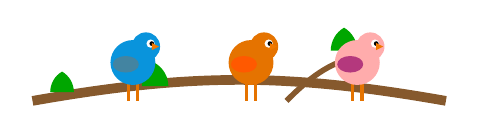
\begin{tikzpicture}[scale=0.75, baseline=(current bounding box.center)]
  % Cành cây
  \draw[line width=3.5pt, brown!70!black] (-3.5,-0.2) to[out=10,in=170] (3.5,-0.2);
  \draw[line width=2pt, brown!70!black] (0.8,-0.2) to[out=45,in=190] (2.2,0.6);
  % Chiếc lá
  \fill[green!65!black] (-1.2,0.05) arc (0:60:0.45) arc (120:180:0.45) -- cycle;
  \fill[green!65!black] (2.0,0.65) arc (0:60:0.45) arc (120:180:0.45) -- cycle;
  \fill[green!65!black] (-2.8,-0.05) arc (0:60:0.4) arc (120:180:0.4) -- cycle;
  % 3 chú chim xinh xắn
  \foreach \x/\c/\wing in {-1.8/cyan!80!blue/cyan!60!black, 0.2/orange!90!black/orange!70!red, 2.0/pink!90!red/magenta!70!black} {
    % Chân chim
    \draw[line width=1.2pt, orange!90!black] (\x-0.08,0.1) -- (\x-0.08,-0.2);
    \draw[line width=1.2pt, orange!90!black] (\x+0.08,0.1) -- (\x+0.08,-0.2);
    % Thân chim
    \fill[\c] (\x,0.45) circle (0.38cm);
    % Cánh chim
    \fill[\wing] (\x-0.12,0.42) ellipse (0.22cm and 0.14cm);
    % Đầu chim
    \fill[\c] (\x+0.22,0.72) circle (0.24cm);
    % Mắt chim
    \fill[white] (\x+0.3,0.77) circle (0.07cm);
    \fill[black] (\x+0.32,0.77) circle (0.04cm);
    % Mỏ chim
    \fill[orange!95!black] (\x+0.44,0.72) -- (\x+0.32,0.66) -- (\x+0.32,0.78) -- cycle;
  }
\end{tikzpicture}
\end{center}
\choice
{$2$}
{$4$}
{$5$}
{\True $3$}
\loigiai{
Đếm lần lượt từng chú chim đậu trên cành: có $1, 2, 3$ chú chim.\\
Số tương ứng là số $3$.\\
\textbf{Đáp án của câu hỏi là D}
}
\end{ex}

% --- CÂU 2 ---
\begin{ex} %[1D1N01]
Trong đĩa không có quả táo nào. Số quả táo trong chiếc đĩa tương ứng với chữ số nào?
\begin{center}
\begin{tikzpicture}[scale=0.8, baseline=(current bounding box.center)]
  % Chiếc đĩa tròn trống
  \draw[fill=cyan!10, draw=cyan!60!blue, line width=1.5pt] (0,0) ellipse (2.6cm and 0.8cm);
  \draw[fill=white, draw=cyan!40, line width=1pt] (0,-0.1) ellipse (2.1cm and 0.55cm);
  \node[font=\small\bfseries\itshape, text=gray!80!black] at (0,-0.1) {(Đĩa trống)};
\end{tikzpicture}
\end{center}
\choice
{\True $0$}
{$1$}
{$2$}
{$3$}
\loigiai{
Trong đĩa hoàn toàn không có quả táo nào, nghĩa là có $0$ quả táo.\\
Số không được viết bằng chữ số là $0$.\\
\textbf{Đáp án của câu hỏi là A}
}
\end{ex}

% --- CÂU 3 ---
\begin{ex} %[1D1H01]
Đoàn tàu hỏa đang chạy theo thứ tự từ bé đến lớn. Toa tàu liền sau toa số $3$ mang số nào?
\begin{center}
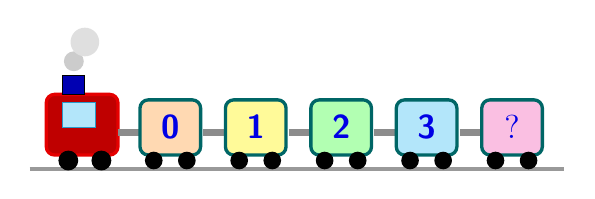
\begin{tikzpicture}[scale=0.7, baseline=(current bounding box.center)]
  % Đường ray
  \draw[line width=1.5pt, gray!80] (-4.5,-0.55) -- (5.2,-0.55);
  % Đầu tàu
  \draw[fill=red!75!black, draw=red!90!black, line width=1.2pt, rounded corners=3pt] (-4.2,-0.3) rectangle (-2.9,0.8);
  \draw[fill=cyan!30, draw=cyan!80!black] (-3.9,0.2) rectangle (-3.3,0.65); % cửa sổ đầu tàu
  \draw[fill=blue!70!black] (-3.9,0.8) rectangle (-3.5,1.15); % ống khói
  \fill[gray!40] (-3.7,1.4) circle (0.18);
  \fill[gray!25] (-3.5,1.75) circle (0.26);
  \fill[black] (-3.8,-0.4) circle (0.18); \fill[black] (-3.2,-0.4) circle (0.18);
  % Nối các toa
  \foreach \i/\num/\cl in {0/0/orange!30, 1/1/yellow!40, 2/2/green!30, 3/3/cyan!30, 4/{$\mathbf{?}$}/magenta!25} {
    \draw[line width=2.5pt, gray!90] (-2.9+\i*1.55,0.1) -- (-2.5+\i*1.55,0.1);
    \draw[fill=\cl, draw=teal!80!black, line width=1.2pt, rounded corners=3pt] (-2.5+\i*1.55,-0.3) rectangle (-1.4+\i*1.55,0.7);
    \node[font=\large\bfseries, text=blue!90!black] at (-1.95+\i*1.55, 0.2) {\num};
    \fill[black] (-2.25+\i*1.55,-0.4) circle (0.16);
    \fill[black] (-1.65+\i*1.55,-0.4) circle (0.16);
  }
\end{tikzpicture}
\end{center}
\choice
{$2$}
{\True $4$}
{$5$}
{$1$}
\loigiai{
Các số xếp theo thứ tự: $0, 1, 2, 3, 4, 5$.\\
Số đứng liền sau số $3$ là số $4$.\\
\textbf{Đáp án của câu hỏi là B}
}
\end{ex}

% --- CÂU 4 ---
\begin{ex} %[1D1H01]
Chú ếch nhảy qua các phiến lá sen mang số $0, \boxed{?}, 2, 3, 4, 5$. Chiếc lá sen đứng liền trước số $2$ mang số mấy?
\begin{center}
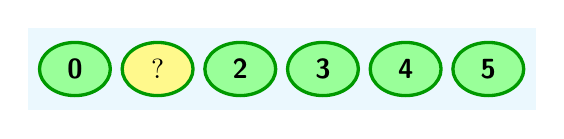
\begin{tikzpicture}[scale=0.75, baseline=(current bounding box.center)]
  % Mặt nước xanh
  \fill[cyan!8] (-0.8,-0.7) rectangle (7.8,0.7);
  % 6 phiến lá sen
  \foreach \x/\num/\col in {0/0/green!40, 1.4/{$\mathbf{?}$}/yellow!45, 2.8/2/green!40, 4.2/3/green!40, 5.6/4/green!40, 7.0/5/green!40} {
    \draw[fill=\col, draw=green!60!black, line width=1.2pt] (\x,0) ellipse (0.6cm and 0.45cm);
    \node[font=\bfseries\normalsize, text=black] at (\x,0) {\num};
  }
\end{tikzpicture}
\end{center}
\choice
{\True $1$}
{$0$}
{$3$}
{$4$}
\loigiai{
Đếm theo dãy số: $0, 1, 2, 3, 4, 5$.\\
Số đứng liền trước số $2$ là số $1$.\\
\textbf{Đáp án của câu hỏi là A}
}
\end{ex}

% --- CÂU 5 ---
\begin{ex} %[1D1H01]
Ba bạn gấu cầm các quả bóng bay mang số $2$, $\boxed{?}$, $4$. Quả bóng bay ở giữa mang số nào?
\begin{center}
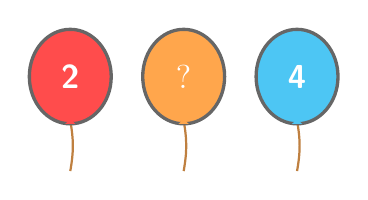
\begin{tikzpicture}[scale=0.8, baseline=(current bounding box.center)]
  \foreach \x/\num/\c in {-1.8/2/red!70, 0/{$\mathbf{?}$}/orange!70, 1.8/4/cyan!70} {
    % Dây bóng
    \draw[line width=0.8pt, brown] (\x,-1.0) to[out=80,in=-80] (\x,-0.2);
    % Quả bóng bay
    \draw[fill=\c, draw=black!60, line width=1.2pt] (\x,0.5) ellipse (0.65cm and 0.75cm);
    \fill[\c] (\x-0.08,-0.25) -- (\x+0.08,-0.25) -- (\x,-0.18) -- cycle;
    \node[font=\large\bfseries, text=white] at (\x,0.5) {\num};
  }
\end{tikzpicture}
\end{center}
\choice
{$1$}
{$5$}
{$0$}
{\True $3$}
\loigiai{
Dãy số liên tiếp: $2, 3, 4$.\\
Số đứng ở giữa số $2$ và số $4$ là số $3$.\\
\textbf{Đáp án của câu hỏi là D}
}
\end{ex}

% --- CÂU 6 ---
\begin{ex} %[1D1H01]
Dãy thẻ số nào dưới đây được xếp theo thứ tự từ bé đến lớn?
\begin{center}
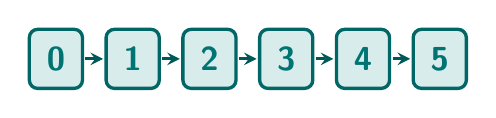
\begin{tikzpicture}[scale=0.75, baseline=(current bounding box.center)]
  \foreach \i/\num in {0/0, 1/1, 2/2, 3/3, 4/4, 5/5} {
    \draw[fill=teal!15, draw=teal!80!black, line width=1.2pt, rounded corners=3pt] (\i*1.3,-0.4) rectangle (\i*1.3+0.9,0.6);
    \node[font=\large\bfseries, text=teal!90!black] at (\i*1.3+0.45, 0.1) {\num};
    \ifnum\i<5
      \draw[->, >=stealth, line width=1pt, teal!70!black] (\i*1.3+0.95,0.1) -- (\i*1.3+1.25,0.1);
    \fi
  }
\end{tikzpicture}
\end{center}
\choice
{$5, 4, 3, 2, 1, 0$}
{\True $0, 1, 2, 3, 4, 5$}
{$1, 3, 2, 4, 5, 0$}
{$0, 2, 1, 3, 5, 4$}
\loigiai{
Dãy số đúng từ bé đến lớn bắt đầu từ số 0 là: $0, 1, 2, 3, 4, 5$.\\
\textbf{Đáp án của câu hỏi là B}
}
\end{ex}

% --- CÂU 7 ---
\begin{ex} %[1D1V01]
Đếm số ngón tay đang xòe ra ở bàn tay dưới đây:
\begin{center}
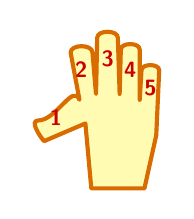
\begin{tikzpicture}[scale=0.75, baseline=(current bounding box.center)]
  % Bàn tay xòe 5 ngón
  \draw[fill=yellow!30, draw=orange!85!black, line width=1.5pt, line join=round]
    (0,-0.6) -- (-0.1,0.5) 
    -- (-0.8,0.2) to[out=130,in=180] (-0.9,0.55) to[out=0,in=110] (-0.2,0.9) % ngón cái
    -- (-0.35,1.7) to[out=90,in=90] (0.02,1.7) -- (0.08,1.0) % ngón trỏ
    -- (0.1,1.95) to[out=90,in=90] (0.45,1.95) -- (0.48,1.0) % ngón giữa
    -- (0.5,1.75) to[out=90,in=90] (0.82,1.75) -- (0.82,0.9) % ngón áp út
    -- (0.85,1.4) to[out=90,in=90] (1.15,1.4) -- (1.1,0.3) % ngón út
    -- (0.9,-0.6) -- cycle;
  % Đánh số ngón tay
  \node[font=\footnotesize\bfseries, text=red!80!black] at (-0.6,0.6) {1};
  \node[font=\footnotesize\bfseries, text=red!80!black] at (-0.17,1.4) {2};
  \node[font=\footnotesize\bfseries, text=red!80!black] at (0.28,1.6) {3};
  \node[font=\footnotesize\bfseries, text=red!80!black] at (0.66,1.4) {4};
  \node[font=\footnotesize\bfseries, text=red!80!black] at (1.0,1.1) {5};
\end{tikzpicture}
\end{center}
\choice
{\True $5$ ngón}
{$4$ ngón}
{$3$ ngón}
{$6$ ngón}
\loigiai{
Đếm lần lượt từng ngón tay: có đúng $5$ ngón tay.\\
\textbf{Đáp án của câu hỏi là A}
}
\end{ex}

% --- CÂU 8 ---
\begin{ex} %[1D1V01]
Có bao nhiêu chú cá đang tung tăng bơi lội trong bình cá?
\begin{center}
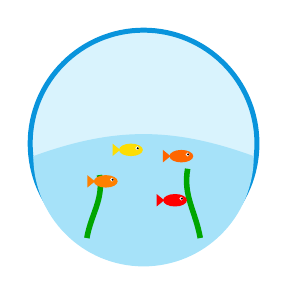
\begin{tikzpicture}[scale=0.8, baseline=(current bounding box.center)]
  % Bình cá tròn
  \draw[fill=cyan!15, draw=cyan!80!blue, line width=1.8pt] (0,0) circle (1.8cm);
  % Mặt nước uốn lượn
  \fill[cyan!35] (-1.75,-0.2) to[out=20,in=160] (1.75,-0.2) arc (0:-180:1.75cm) -- cycle;
  % Cây thủy sinh
  \draw[green!65!black, line width=2pt] (-0.9,-1.5) to[out=80,in=-80] (-0.7,-0.5);
  \draw[green!65!black, line width=2pt] (0.9,-1.5) to[out=100,in=-100] (0.7,-0.4);
  % 4 chú cá xinh
  \foreach \px/\py/\c in {-0.6/-0.6/orange, 0.5/-0.9/red, -0.2/-0.1/yellow!80!orange, 0.6/-0.2/orange!80!red} {
    \begin{scope}[shift={(\px,\py)}, scale=0.45]
      \fill[\c] (0,0) ellipse (0.42cm and 0.22cm);
      \fill[\c] (-0.38,0) -- (-0.65,0.22) -- (-0.65,-0.22) -- cycle; % đuôi cá
      \fill[white] (0.22,0.06) circle (0.07cm);
      \fill[black] (0.24,0.06) circle (0.04cm);
    \end{scope}
  }
\end{tikzpicture}
\end{center}
\choice
{$3$ chú cá}
{$5$ chú cá}
{\True $4$ chú cá}
{$2$ chú cá}
\loigiai{
Đếm trong bình: có $1, 2, 3, 4$ chú cá đang bơi.\\
Số lượng chú cá là $4$.\\
\textbf{Đáp án của câu hỏi là C}
}
\end{ex}

% --- CÂU 9 ---
\begin{ex} %[1D1V01]
Lan có $2$ cái bút chì màu vàng, mẹ cho Lan thêm $2$ cái bút chì màu xanh. Đếm tất cả có bao nhiêu cái bút chì?
\begin{center}
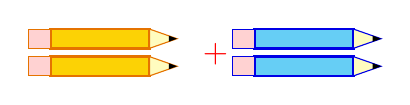
\begin{tikzpicture}[scale=0.7, baseline=(current bounding box.center)]
  % Nhóm 2 bút vàng
  \foreach \y in {0.5, 0} {
    \draw[fill=yellow!70!orange, draw=orange!90!black, line width=1pt] (-3,\y) rectangle (-1.2,\y+0.35);
    \draw[fill=pink!70, draw=orange!90!black] (-3.4,\y) rectangle (-3,\y+0.35); % tẩy
    \draw[fill=yellow!25, draw=orange!90!black] (-1.2,\y) -- (-0.7,\y+0.175) -- (-1.2,\y+0.35) -- cycle;
    \fill[black] (-0.85,\y+0.12) -- (-0.7,\y+0.175) -- (-0.85,\y+0.23) -- cycle;
  }
  \node[font=\large\bfseries, text=red] at (0,0.4) {$+$};
  % Nhóm 2 bút xanh
  \foreach \y in {0.5, 0} {
    \draw[fill=cyan!60, draw=blue!90!black, line width=1pt] (0.7,\y) rectangle (2.5,\y+0.35);
    \draw[fill=pink!70, draw=blue!90!black] (0.3,\y) rectangle (0.7,\y+0.35); % tẩy
    \draw[fill=yellow!25, draw=blue!90!black] (2.5,\y) -- (3.0,\y+0.175) -- (2.5,\y+0.35) -- cycle;
    \fill[black] (2.85,\y+0.12) -- (3.0,\y+0.175) -- (2.85,\y+0.23) -- cycle;
  }
\end{tikzpicture}
\end{center}
\choice
{$3$ cái}
{$5$ cái}
{\True $4$ cái}
{$2$ cái}
\loigiai{
Đếm tất cả số bút chì: $2$ cái bút vàng và $2$ cái bút xanh là $4$ cái bút chì.\\
\textbf{Đáp án của câu hỏi là C}
}
\end{ex}

% --- CÂU 10 ---
\begin{ex} %[1D1V01]
Trong chùm bóng bay mang số $4, 2, 0, 5, 3$ dưới đây, quả bóng nào mang số \textbf{bé nhất}?
\begin{center}
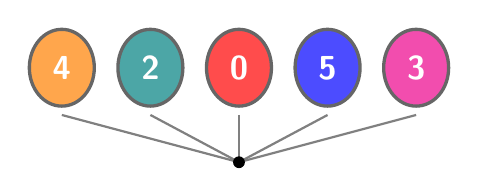
\begin{tikzpicture}[scale=0.75, baseline=(current bounding box.center)]
  \foreach \x/\num/\c in {-3/4/orange, -1.5/2/teal, 0/0/red, 1.5/5/blue, 3/3/magenta} {
    \draw[line width=0.8pt, gray] (\x,-0.8) -- (0,-1.6);
    \draw[fill=\c!70, draw=black!60, line width=1.2pt] (\x,0) ellipse (0.55cm and 0.65cm);
    \node[font=\large\bfseries, text=white] at (\x,0) {\num};
  }
  \fill[black] (0,-1.6) circle (0.1cm);
\end{tikzpicture}
\end{center}
\choice
{$2$}
{\True $0$}
{$3$}
{$4$}
\loigiai{
Trong các số $4, 2, 0, 5, 3$, số bé nhất là số $0$.\\
\textbf{Đáp án của câu hỏi là B}
}
\end{ex}

% --- CÂU 11 ---
\begin{ex} %[1D1V01]
Trong các ngôi sao mang số $1, 4, 3, 5, 2$, ngôi sao nào mang số \textbf{lớn nhất}?
\begin{center}

\begin{tikzpicture}[scale=0.75, baseline=(current bounding box.center)]
  \foreach \x/\num in {-3/1, -1.5/4, 0/3, 1.5/5, 3/2} {
    \node[draw=orange!80!black, fill=yellow!80, star, star points=5, star point ratio=2.2, line width=1.2pt, minimum size=1.1cm] at (\x,0) {};
    \node[font=\bfseries\normalsize, text=red!85!black] at (\x,-0.02) {\num};
  }
\end{tikzpicture}
\end{center}
\choice
{$4$}
{$3$}
{$1$}
{\True $5$}
\loigiai{
So sánh các số: $1 < 2 < 3 < 4 < 5$. Số lớn nhất là số $5$.\\
\textbf{Đáp án của câu hỏi là D}
}
\end{ex}

% --- CÂU 12 ---
\begin{ex} %[1D1C01]
Chú sâu đo ngộ nghĩnh có các đốt mang số: $0, 1, \dots, 3, 4, 5$. Số còn thiếu ở dấu $\mathbf{?}$ là số nào?
\begin{center}
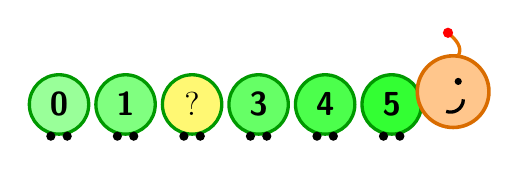
\begin{tikzpicture}[scale=0.65, baseline=(current bounding box.center)]
  \foreach \x/\num/\c in {0/0/green!40, 1.3/1/green!50, 2.6/{$\mathbf{?}$}/yellow!55, 3.9/3/green!60, 5.2/4/green!70, 6.5/5/green!80} {
    \draw[fill=\c, draw=green!60!black, line width=1.2pt] (\x,0) circle (0.58cm);
    \node[font=\large\bfseries, text=black] at (\x,0) {\num};
    \fill[black] (\x-0.16,-0.62) circle (0.09); \fill[black] (\x+0.16,-0.62) circle (0.09);
  }
  % Đầu sâu
  \draw[fill=orange!45, draw=orange!85!black, line width=1.3pt] (7.7,0.25) circle (0.7cm);
  \fill[black] (7.8,0.45) circle (0.07); % mắt
  \draw[line width=1.2pt] (7.9,0.1) arc (0:-110:0.25); % cười
  \draw[line width=1.2pt, orange!90!black] (7.8,0.95) to[out=60,in=-40] (7.6,1.4); % râu
  \fill[red] (7.6,1.4) circle (0.1);
\end{tikzpicture}
\end{center}
\choice
{$1$}
{$3$}
{\True $2$}
{$4$}
\loigiai{
Đếm dãy số từ $0$ đến $5$: $0, 1, 2, 3, 4, 5$.\\
Số còn thiếu ở giữa số 1 và số 3 là số $2$.\\
\textbf{Đáp án của câu hỏi là C}
}
\end{ex}

% =========================================================================
% PHẦN 2: TRẮC NGHIỆM ĐÚNG SAI (QUAN SÁT TRANH MINH HỌA)
% =========================================================================
\textbf{Phần 2. Trắc nghiệm đúng sai (Quan sát tranh và xét tính đúng/sai)}
\setcounterpageref{ex}{0}

% --- CÂU 13 ---
\begin{ex} %[1D1H01]
Quan sát tia số từ $0$ đến $5$ với các bước nhảy của chú cào cào:
\begin{center}
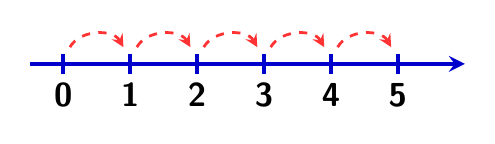
\begin{tikzpicture}[scale=0.85, baseline=(current bounding box.center)]
  % Tia số
  \draw[->, >=stealth, line width=1.5pt, blue!80!black] (-0.5,0) -- (6.0,0);
  \foreach \x in {0,1,2,3,4,5} {
    \draw[line width=1.5pt, blue!80!black] (\x,0.15) -- (\x,-0.15);
    \node[font=\bfseries\large, below] at (\x,-0.15) {\x};
  }
  % Các bước nhảy vòng cung
  \foreach \x in {0,1,2,3,4} {
    \draw[->, >=stealth, dashed, line width=1pt, red!80] (\x+0.1,0.25) to[out=60,in=120] (\x+0.9,0.25);
  }
\end{tikzpicture}
\end{center}
Xét tính đúng sai của các câu sau:
\choiceTF
{\True Số $0$ là số bé nhất trong các số từ $0$ đến $5$.}
{\True Số $5$ là số lớn nhất trong các số từ $0$ đến $5$.}
{Số $3$ đứng liền sau số $4$.}
{\True Số $3$ đứng liền trước số $4$.}
\loigiai{
\begin{itemize}
    \item Số $0$ ở vị trí đầu tiên bên trái nên là số bé nhất: \textbf{Đúng}.
    \item Số $5$ ở vị trí ngoài cùng bên phải nên là số lớn nhất: \textbf{Đúng}.
    \item Số $3$ đứng trước số $4$, không phải đứng sau: \textbf{Sai}.
    \item Số $3$ đứng liền trước số $4$: \textbf{Đúng}.
\end{itemize}
}
\end{ex}

% --- CÂU 14 ---
\begin{ex} %[1D1V01]
Quan sát bức tranh nông trại có các nhóm đồ vật sau:
\begin{center}
\begin{tikzpicture}[scale=0.7, baseline=(current bounding box.center)]
  % Ô 1: 1 chú gà trống
  \draw[fill=yellow!15, draw=orange!70, line width=1pt, rounded corners=4pt] (-4.8,-1) rectangle (-2.2,1.2);
  \node[font=\small\bfseries, text=orange!90!black] at (-3.5,0.9) {Gà trống};
  \fill[orange!90!black] (-3.5,0) circle (0.35cm);
  \fill[red] (-3.4,0.3) circle (0.15cm); % mào
  \node[font=\bfseries] at (-3.5,-0.6) {1 con};

  % Ô 2: 3 quả táo
  \draw[fill=red!10, draw=red!70, line width=1pt, rounded corners=4pt] (-1.8,-1) rectangle (1.2,1.2);
  \node[font=\small\bfseries, text=red!90!black] at (-0.3,0.9) {Quả táo};
  \foreach \x in {-1.0, -0.3, 0.4} {
    \fill[red!80!black] (\x,0) circle (0.28cm);
    \fill[green!70!black] (\x,0.28) circle (0.08cm);
  }
  \node[font=\bfseries] at (-0.3,-0.6) {3 quả};

  % Ô 3: 5 bông hoa
  \draw[fill=pink!15, draw=magenta!70, line width=1pt, rounded corners=4pt] (1.6,-1) rectangle (5.2,1.2);
  \node[font=\small\bfseries, text=magenta!90!black] at (3.4,0.9) {Bông hoa};
  \foreach \x in {2.1, 2.75, 3.4, 4.05, 4.7} {
    \fill[magenta!70] (\x,0.05) circle (0.22cm);
    \fill[yellow] (\x,0.05) circle (0.1cm);
  }
  \node[font=\bfseries] at (3.4,-0.6) {5 bông};
\end{tikzpicture}
\end{center}
Xét tính đúng sai của các câu sau:
\choiceTF
{\True Số lượng gà trống là $1$ con.}
{\True Số quả táo là $3$ quả.}
{Số quả táo nhiều hơn số bông hoa.}
{\True Nhóm bông hoa có số lượng nhiều nhất ($5$ bông).}
\loigiai{
\begin{itemize}
    \item Có $1$ chú gà trống: \textbf{Đúng}.
    \item Có $3$ quả táo: \textbf{Đúng}.
    \item $3$ quả táo ít hơn $5$ bông hoa (nói nhiều hơn là sai): \textbf{Sai}.
    \item Nhóm bông hoa có 5 bông là nhiều nhất: \textbf{Đúng}.
\end{itemize}
}
\end{ex}

% =========================================================================
% PHẦN 3: TRẢ LỜI NGẮN (ĐIỀN SỐ THÍCH HỢP VÀO Ô TRỐNG)
% =========================================================================
\textbf{Phần 3. Trả lời ngắn (Quan sát hình vẽ và điền số thích hợp)}
\setcounterpageref{ex}{0}

% --- CÂU 15 ---
\begin{ex} %[1D1H01]
Đếm số quả dâu tây trên chiếc đĩa dưới đây:
\begin{center}
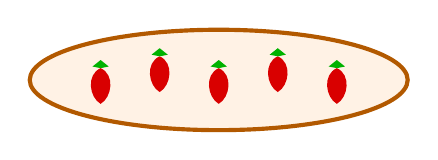
\begin{tikzpicture}[scale=0.75, baseline=(current bounding box.center)]
  % Chiếc đĩa
  \draw[fill=orange!10, draw=orange!70!black, line width=1.5pt] (0,-0.2) ellipse (3.2cm and 0.85cm);
  % 5 quả dâu tây
  \foreach \x/\y in {-2.0/0, -1.0/0.2, 0/0, 1.0/0.2, 2.0/0} {
    \begin{scope}[shift={(\x,\y)}, scale=0.55]
      \fill[red!85!black] (0,0) .. controls (-0.45,-0.2) and (-0.35,-0.9) .. (0,-1.1) .. controls (0.35,-0.9) and (0.45,-0.2) .. (0,0);
      \fill[green!70!black] (-0.25,0.05) -- (0,0) -- (0.25,0.05) -- (0,0.25) -- cycle;
    \end{scope}
  }
\end{tikzpicture}
\end{center}
\shortans{5}
\loigiai{
\textbf{Đáp số:} $5$\\
Đếm trên đĩa có $1, 2, 3, 4, 5$ quả dâu tây.
}
\end{ex}

% --- CÂU 16 ---
\begin{ex} %[1D1H01]
Quan sát sơ đồ tách - gộp số: Số $5$ gồm $3$ và mấy?
\begin{center}
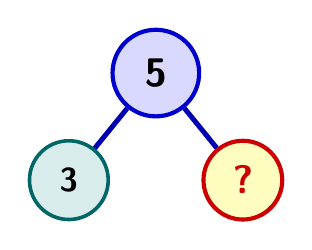
\begin{tikzpicture}[scale=0.85, baseline=(current bounding box.center)]
  % Quả to ở trên
  \node[draw=blue!80!black, circle, fill=blue!15, line width=1.5pt, minimum size=1.1cm, font=\bfseries\Large] (Tong) at (0,1.2) {5};
  % Hai nhánh ở dưới
  \node[draw=teal!80!black, circle, fill=teal!15, line width=1.3pt, minimum size=1cm, font=\bfseries\large] (N1) at (-1.3,-0.4) {3};
  \node[draw=red!80!black, circle, fill=yellow!25, line width=1.5pt, minimum size=1cm, font=\bfseries\Large, text=red!80!black] (N2) at (1.3,-0.4) {?};
  % Đường nối
  \draw[line width=1.8pt, blue!70!black] (Tong) -- (N1);
  \draw[line width=1.8pt, blue!70!black] (Tong) -- (N2);
\end{tikzpicture}
\end{center}
\shortans{2}
\loigiai{
\textbf{Đáp số:} $2$\\
Tách số: $5$ gồm $3$ và $2$.
}
\end{ex}

% --- CÂU 17 ---
\begin{ex} %[1D1V01]
Có bao nhiêu chiếc bánh kem thơm ngon trong hộp dưới đây?
\begin{center}
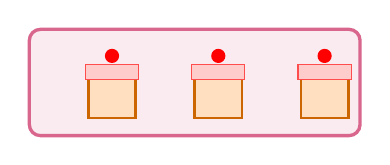
\begin{tikzpicture}[scale=0.75, baseline=(current bounding box.center)]
  \draw[fill=purple!8, draw=purple!60, line width=1.2pt, rounded corners=4pt] (-2.8,-0.8) rectangle (2.8,1.0);
  \foreach \x in {-1.8, 0, 1.8} {
    % Chiếc bánh
    \draw[fill=orange!25, draw=orange!80!black, line width=1pt] (\x,-0.5) rectangle (\x+0.8,0.2);
    \draw[fill=pink!80, draw=red!70] (\x-0.05,0.15) rectangle (\x+0.85,0.4);
    \fill[red] (\x+0.4,0.55) circle (0.12cm); % quả cherry
  }
\end{tikzpicture}
\end{center}
\shortans{3}
\loigiai{
\textbf{Đáp số:} $3$\\
Đếm trong hộp có đúng $3$ chiếc bánh kem.
}
\end{ex}

% --- CÂU 18 ---
\begin{ex} %[1D1V01]
Điền số còn thiếu vào chiếc lá sen có dấu $\mathbf{?}$:
\begin{center}
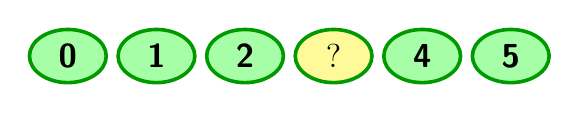
\begin{tikzpicture}[scale=0.75, baseline=(current bounding box.center)]
  \foreach \x/\num/\col in {0/0/green!35, 1.5/1/green!35, 3.0/2/green!35, 4.5/{$\mathbf{?}$}/yellow!40, 6.0/4/green!35, 7.5/5/green!35} {
    \draw[fill=\col, draw=green!60!black, line width=1.3pt] (\x,0) ellipse (0.65cm and 0.45cm);
    \node[font=\large\bfseries, text=black] at (\x,0) {\num};
  }
\end{tikzpicture}
\end{center}
\shortans{3}
\loigiai{
\textbf{Đáp số:} $3$\\
Thứ tự các số: $0, 1, 2, 3, 4, 5$. Số còn thiếu là $3$.
}
\end{ex}

% --- CÂU 19 ---
\begin{ex} %[1D1V01]
Có $3$ chú bướm tím đang bay lượn, có thêm $1$ chú bướm vàng bay tới. Hỏi có tất cả bao nhiêu chú bướm?
\begin{center}

\begin{tikzpicture}[scale=0.7, baseline=(current bounding box.center)]
  % 3 chú bướm tím
  \foreach \x/\y in {-3.2, -1.8, -0.4} {
    \begin{scope}[shift={(\x,0.2)}, scale=0.5]
      \fill[magenta!70!purple] (-0.2,0.2) ellipse (0.4 and 0.6);
      \fill[magenta!70!purple] (0.2,0.2) ellipse (0.4 and 0.6);
      \fill[pink!80] (-0.2,-0.3) ellipse (0.3 and 0.4);
      \fill[pink!80] (0.2,-0.3) ellipse (0.3 and 0.4);
      \fill[black] (0,0) ellipse (0.1 and 0.5);
    \end{scope}
  }
  \node[font=\Large\bfseries, text=red] at (0.8,0.2) {$+$};
  % 1 chú bướm vàng
  \begin{scope}[shift={(2.2,0.2)}, scale=0.5]
    \fill[yellow!90!orange] (-0.2,0.2) ellipse (0.4 and 0.6);
    \fill[yellow!90!orange] (0.2,0.2) ellipse (0.4 and 0.6);
    \fill[orange!80] (-0.2,-0.3) ellipse (0.3 and 0.4);
    \fill[orange!80] (0.2,-0.3) ellipse (0.3 and 0.4);
    \fill[black] (0,0) ellipse (0.1 and 0.5);
  \end{scope}
\end{tikzpicture}
\end{center}
\shortans{4}
\loigiai{
\textbf{Đáp số:} $4$\\
Gộp $3$ chú bướm và $1$ chú bướm là có tất cả $4$ chú bướm.
}
\end{ex}

% --- CÂU 20 ---
\begin{ex} %[1D1V01]
Trong chuồng không có chú gà nào. Hãy viết chữ số tương ứng với số chú gà trong chuồng:
\begin{center}
\begin{tikzpicture}[scale=0.75, baseline=(current bounding box.center)]
  % Hàng rào gỗ chuồng gà trống
  \draw[line width=3pt, brown!70!black] (-2.5,0.3) -- (2.5,0.3);
  \draw[line width=3pt, brown!70!black] (-2.5,-0.3) -- (2.5,-0.3);
  \foreach \x in {-2.0, -1.0, 0, 1.0, 2.0} {
    \draw[line width=4pt, brown!90!black] (\x,-0.6) -- (\x,0.7);
  }
  \node[font=\small\bfseries\itshape, text=gray!80!black] at (0,-1.0) {(Chuồng trống)};
\end{tikzpicture}
\end{center}
\shortans{0}
\loigiai{
\textbf{Đáp số:} $0$\\
Trong chuồng không có chú gà nào nghĩa là số $0$.
}
\end{ex}

\newpage

\subsection*{Bài 02. Các số 6, 7, 8, 9, 10}
\addcontentsline{toc}{subsection}{Bài 02. Các số 6, 7, 8, 9, 10}
\TaoPhieuKiemTra{Chủ đề 1 -- Các số từ 0 đến 10}{02}{Các số 6, 7, 8, 9, 10}{https://loptoanthaylinh.vn/thi-online/toan-1/bai-02}
\textbf{Phần 1. Trắc nghiệm lựa chọn (Học sinh quan sát hình và chọn đáp án đúng)}
\setcounterpageref{ex}{0}

% --- CÂU 1 ---
\begin{ex} %[1D1N02]
Đếm số chấm tròn trong khung dưới đây và cho biết số mười được viết bằng chữ số nào?
\begin{center}
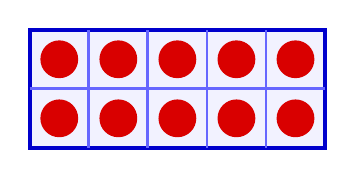
\begin{tikzpicture}[scale=0.75, baseline=(current bounding box.center)]
  % Khung 10 ô (2 hàng 5 cột)
  \draw[line width=1.5pt, blue!80!black, fill=blue!5] (0,0) rectangle (5,2);
  \draw[line width=1pt, blue!60] (0,1) -- (5,1);
  \foreach \x in {1,2,3,4} {
    \draw[line width=1pt, blue!60] (\x,0) -- (\x,2);
  }
  % 10 chấm tròn đỏ
  \foreach \x in {0.5, 1.5, 2.5, 3.5, 4.5} {
    \fill[red!85!black] (\x, 1.5) circle (0.32cm);
    \fill[red!85!black] (\x, 0.5) circle (0.32cm);
  }
\end{tikzpicture}
\end{center}
\choice
{\True $10$}
{$1$}
{$01$}
{$100$}
\loigiai{
Trong khung có đúng $10$ chấm tròn đỏ.\\
Số mười được viết bằng chữ số là $10$.\\
\textbf{Đáp án của câu hỏi là A}
}
\end{ex}

% --- CÂU 2 ---
\begin{ex} %[1D1N02]
Chú chim nhỏ đang đậu ở cành số $6$, cành cây liền sau mang số mấy?
\begin{center}
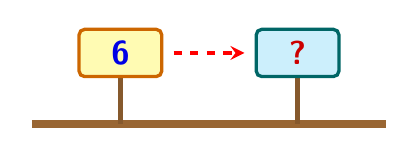
\begin{tikzpicture}[scale=0.75, baseline=(current bounding box.center)]
  \draw[line width=3pt, brown!80!black] (-3,0) -- (3,0);
  % 2 cành rẽ nhánh
  \draw[line width=2pt, brown!70!black] (-1.5,0) -- (-1.5,1.2);
  \draw[line width=2pt, brown!70!black] (1.5,0) -- (1.5,1.2);
  % Biển số
  \draw[fill=yellow!30, draw=orange!80!black, line width=1.2pt, rounded corners=2pt] (-2.2,0.8) rectangle (-0.8,1.6);
  \node[font=\large\bfseries, text=blue!90!black] at (-1.5,1.2) {6};
  \draw[fill=cyan!20, draw=teal!80!black, line width=1.2pt, rounded corners=2pt] (0.8,0.8) rectangle (2.2,1.6);
  \node[font=\large\bfseries, text=red!80!black] at (1.5,1.2) {?};
  \draw[->, >=stealth, dashed, line width=1.2pt, red] (-0.6,1.2) -- (0.6,1.2);
\end{tikzpicture}
\end{center}
\choice
{$5$}
{$8$}
{\True $7$}
{$9$}
\loigiai{
Đếm số liên tiếp: $6, 7, 8, \dots$\\
Số đứng liền sau của số $6$ là số $7$.\\
\textbf{Đáp án của câu hỏi là C}
}
\end{ex}

% --- CÂU 3 ---
\begin{ex} %[1D1H02]
Đoàn tàu chở các số từ $6$ đến $10$. Toa tàu đứng liền trước số $10$ mang số mấy?
\begin{center}
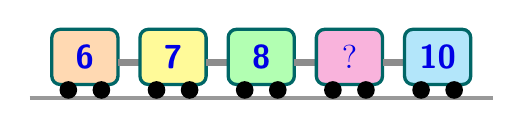
\begin{tikzpicture}[scale=0.7, baseline=(current bounding box.center)]
  \draw[line width=1.5pt, gray!80] (-4.2,-0.55) -- (4.2,-0.55);
  % 5 toa
  \foreach \i/\num/\cl in {0/6/orange!30, 1/7/yellow!40, 2/8/green!30, 3/{$\mathbf{?}$}/magenta!30, 4/10/cyan!30} {
    \draw[fill=\cl, draw=teal!80!black, line width=1.2pt, rounded corners=3pt] (-3.8+\i*1.6,-0.3) rectangle (-2.6+\i*1.6,0.7);
    \node[font=\large\bfseries, text=blue!90!black] at (-3.2+\i*1.6, 0.2) {\num};
    \fill[black] (-3.5+\i*1.6,-0.4) circle (0.16);
    \fill[black] (-2.9+\i*1.6,-0.4) circle (0.16);
    \ifnum\i<4
      \draw[line width=2.5pt, gray!90] (-2.6+\i*1.6,0.1) -- (-2.2+\i*1.6,0.1);
    \fi
  }
\end{tikzpicture}
\end{center}
\choice
{$8$}
{\True $9$}
{$7$}
{$6$}
\loigiai{
Thứ tự các số: $6, 7, 8, 9, 10$.\\
Số đứng liền trước số $10$ là số $9$.\\
\textbf{Đáp án của câu hỏi là B}
}
\end{ex}

% --- CÂU 4 ---
\begin{ex} %[1D1H02]
Ba bạn gấu cầm các quả bóng bay mang số $7$, $\mathbf{?}$, $9$. Quả bóng bay ở giữa mang số nào?
\begin{center}
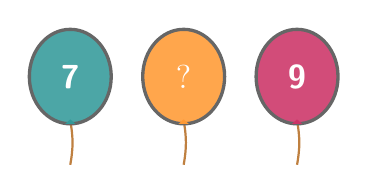
\begin{tikzpicture}[scale=0.8, baseline=(current bounding box.center)]
  \foreach \x/\num/\c in {-1.8/7/teal, 0/{$\mathbf{?}$}/orange, 1.8/9/purple} {
    \draw[line width=0.8pt, brown] (\x,-0.9) to[out=80,in=-80] (\x,-0.2);
    \draw[fill=\c!70, draw=black!60, line width=1.2pt] (\x,0.5) ellipse (0.65cm and 0.75cm);
    \fill[\c!80] (\x-0.08,-0.25) -- (\x+0.08,-0.25) -- (\x,-0.18) -- cycle;
    \node[font=\large\bfseries, text=white] at (\x,0.5) {\num};
  }
\end{tikzpicture}
\end{center}
\choice
{$6$}
{$10$}
{$5$}
{\True $8$}
\loigiai{
Số đứng ở giữa số $7$ và số $9$ là số $8$.\\
\textbf{Đáp án của câu hỏi là D}
}
\end{ex}

% --- CÂU 5 ---
\begin{ex} %[1D1H02]
Đếm ngược từ $10$ về $6$ trên thân chú sâu: $10, 9, 8, \dots, 6$. Đốt thân có dấu $\mathbf{?}$ là số mấy?
\begin{center}
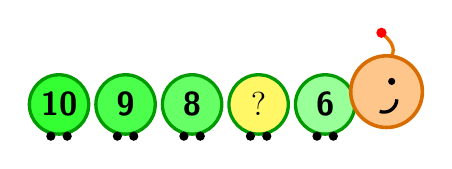
\begin{tikzpicture}[scale=0.65, baseline=(current bounding box.center)]
  \foreach \x/\num/\c in {0/10/green!80, 1.3/9/green!70, 2.6/8/green!60, 3.9/{$\mathbf{?}$}/yellow!60, 5.2/6/green!40} {
    \draw[fill=\c, draw=green!60!black, line width=1.2pt] (\x,0) circle (0.58cm);
    \node[font=\large\bfseries, text=black] at (\x,0) {\num};
    \fill[black] (\x-0.16,-0.62) circle (0.09); \fill[black] (\x+0.16,-0.62) circle (0.09);
  }
  % Đầu sâu
  \draw[fill=orange!45, draw=orange!85!black, line width=1.3pt] (6.4,0.25) circle (0.7cm);
  \fill[black] (6.5,0.45) circle (0.07);
  \draw[line width=1.2pt] (6.6,0.1) arc (0:-110:0.25);
  \draw[line width=1.2pt, orange!90!black] (6.5,0.95) to[out=60,in=-40] (6.3,1.4);
  \fill[red] (6.3,1.4) circle (0.1);
\end{tikzpicture}
\end{center}
\choice
{$6$}
{$8$}
{$9$}
{\True $7$}
\loigiai{
Đếm lùi từ 10 về 6: $10, 9, 8, 7, 6$.\\
Số còn thiếu là số $7$.\\
\textbf{Đáp án của câu hỏi là D}
}
\end{ex}

% --- CÂU 6 ---
\begin{ex} %[1D1H02]
Trong các thẻ số dưới đây, thẻ nào mang số gồm \textbf{hai chữ số}?
\begin{center}
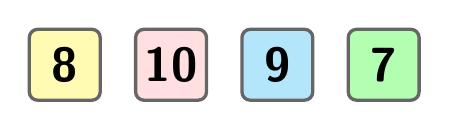
\begin{tikzpicture}[scale=0.75, baseline=(current bounding box.center)]
  \foreach \i/\num/\c in {0/8/yellow!30, 1/10/pink!50, 2/9/cyan!30, 3/7/green!30} {
    \draw[fill=\c, draw=black!60, line width=1.2pt, rounded corners=3pt] (\i*1.8,-0.4) rectangle (\i*1.8+1.2,0.8);
    \node[font=\LARGE\bfseries, text=black] at (\i*1.8+0.6, 0.2) {\num};
  }
\end{tikzpicture}
\end{center}
\choice
{\True $10$}
{$8$}
{$9$}
{$7$}
\loigiai{
Số $10$ được ghép từ hai chữ số: chữ số $1$ và chữ số $0$.\\
Các số $7, 8, 9$ chỉ có một chữ số.\\
\textbf{Đáp án của câu hỏi là A}
}
\end{ex}

% --- CÂU 7 ---
\begin{ex} %[1D1V02]
Hai bàn tay xòe ra dưới đây có tất cả bao nhiêu ngón tay?
\begin{center}
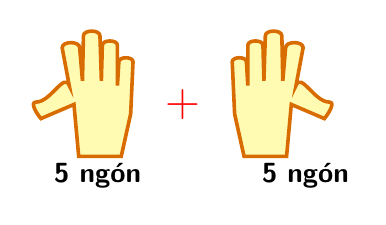
\begin{tikzpicture}[scale=0.6, baseline=(current bounding box.center)]
  % Bàn tay trái
  \begin{scope}[shift={(-2.2,0)}]
    \draw[fill=yellow!30, draw=orange!85!black, line width=1.3pt]
      (0,-0.6) -- (-0.1,0.5) -- (-0.8,0.2) to[out=130,in=180] (-0.9,0.55) to[out=0,in=110] (-0.2,0.9)
      -- (-0.35,1.7) to[out=90,in=90] (0.02,1.7) -- (0.08,1.0)
      -- (0.1,1.95) to[out=90,in=90] (0.45,1.95) -- (0.48,1.0)
      -- (0.5,1.75) to[out=90,in=90] (0.82,1.75) -- (0.82,0.9)
      -- (0.85,1.4) to[out=90,in=90] (1.15,1.4) -- (1.1,0.3)
      -- (0.9,-0.6) -- cycle;
    \node[font=\bfseries] at (0.4,-1.0) {5 ngón};
  \end{scope}
  \node[font=\LARGE\bfseries, text=red] at (0,0.5) {$+$};
  % Bàn tay phải
  \begin{scope}[shift={(2.2,0)}, xscale=-1]
    \draw[fill=yellow!30, draw=orange!85!black, line width=1.3pt]
      (0,-0.6) -- (-0.1,0.5) -- (-0.8,0.2) to[out=130,in=180] (-0.9,0.55) to[out=0,in=110] (-0.2,0.9)
      -- (-0.35,1.7) to[out=90,in=90] (0.02,1.7) -- (0.08,1.0)
      -- (0.1,1.95) to[out=90,in=90] (0.45,1.95) -- (0.48,1.0)
      -- (0.5,1.75) to[out=90,in=90] (0.82,1.75) -- (0.82,0.9)
      -- (0.85,1.4) to[out=90,in=90] (1.15,1.4) -- (1.1,0.3)
      -- (0.9,-0.6) -- cycle;
    \node[font=\bfseries] at (-0.4,-1.0) {5 ngón};
  \end{scope}
\end{tikzpicture}
\end{center}
\choice
{$8$ ngón}
{$9$ ngón}
{\True $10$ ngón}
{$7$ ngón}
\loigiai{
Mỗi bàn tay có 5 ngón, hai bàn tay có tất cả $5 + 5 = 10$ ngón tay.\\
\textbf{Đáp án của câu hỏi là C}
}
\end{ex}

% --- CÂU 8 ---
\begin{ex} %[1D1V02]
Trong chùm bóng bay mang số $6, 9, 7, 10, 8$, quả bóng nào mang số \textbf{lớn nhất}?
\begin{center}
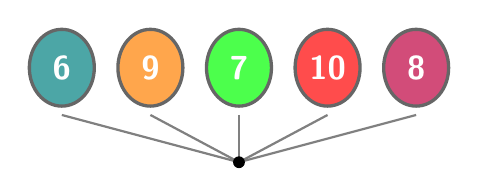
\begin{tikzpicture}[scale=0.75, baseline=(current bounding box.center)]
  \foreach \x/\num/\c in {-3/6/teal, -1.5/9/orange, 0/7/green, 1.5/10/red, 3/8/purple} {
    \draw[line width=0.8pt, gray] (\x,-0.8) -- (0,-1.6);
    \draw[fill=\c!70, draw=black!60, line width=1.2pt] (\x,0) ellipse (0.55cm and 0.65cm);
    \node[font=\large\bfseries, text=white] at (\x,0) {\num};
  }
  \fill[black] (0,-1.6) circle (0.1cm);
\end{tikzpicture}
\end{center}
\choice
{$9$}
{$8$}
{\True $10$}
{$7$}
\loigiai{
So sánh các số: $6 < 7 < 8 < 9 < 10$. Số lớn nhất là $10$.\\
\textbf{Đáp án của câu hỏi là C}
}
\end{ex}

% --- CÂU 9 ---
\begin{ex} %[1D1V02]
Trong các ngôi sao mang số $6, 8, 10, 7, 9$, ngôi sao nào mang số \textbf{bé nhất}?
\begin{center}
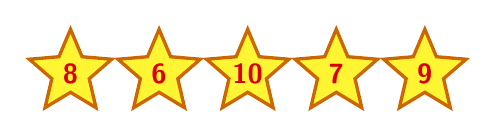
\begin{tikzpicture}[scale=0.75, baseline=(current bounding box.center)]
  \foreach \x/\num in {-3/8, -1.5/6, 0/10, 1.5/7, 3/9} {
    \node[draw=orange!80!black, fill=yellow!80, star, star points=5, star point ratio=2.2, line width=1.2pt, minimum size=1.1cm] at (\x,0) {};
    \node[font=\bfseries\normalsize, text=red!85!black] at (\x,-0.02) {\num};
  }
\end{tikzpicture}
\end{center}
\choice
{\True $6$}
{$7$}
{$8$}
{$9$}
\loigiai{
Trong các số $6, 8, 10, 7, 9$, số bé nhất là số $6$.\\
\textbf{Đáp án của câu hỏi là A}
}
\end{ex}

% --- CÂU 10 ---
\begin{ex} %[1D1V02]
Dãy thẻ số nào dưới đây được xếp đúng theo thứ tự từ bé đến lớn?
\begin{center}
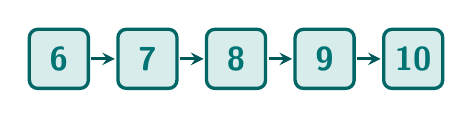
\begin{tikzpicture}[scale=0.75, baseline=(current bounding box.center)]
  \foreach \i/\num in {0/6, 1/7, 2/8, 3/9, 4/10} {
    \draw[fill=teal!15, draw=teal!80!black, line width=1.2pt, rounded corners=3pt] (\i*1.5,-0.4) rectangle (\i*1.5+1.0,0.6);
    \node[font=\large\bfseries, text=teal!90!black] at (\i*1.5+0.5, 0.1) {\num};
    \ifnum\i<4
      \draw[->, >=stealth, line width=1pt, teal!70!black] (\i*1.5+1.05,0.1) -- (\i*1.5+1.45,0.1);
    \fi
  }
\end{tikzpicture}
\end{center}
\choice
{$10, 9, 8, 7, 6$}
{\True $6, 7, 8, 9, 10$}
{$6, 8, 7, 9, 10$}
{$7, 6, 8, 9, 10$}
\loigiai{
Thứ tự đếm xuôi từ bé đến lớn: $6, 7, 8, 9, 10$.\\
\textbf{Đáp án của câu hỏi là B}
}
\end{ex}

% --- CÂU 11 ---
\begin{ex} %[1D1V02]
Có $6$ quả cam trong đĩa, mẹ để thêm $2$ quả cam nữa. Đếm tất cả có bao nhiêu quả cam?
\begin{center}
\begin{tikzpicture}[scale=0.7, baseline=(current bounding box.center)]
  % Đĩa cam có 6 quả
  \draw[fill=orange!10, draw=orange!70!black, line width=1.2pt] (-2.5,-0.2) ellipse (2.2cm and 0.7cm);
  \foreach \x/\y in {-3.5/0, -2.9/0.2, -2.3/0, -1.7/0.2, -2.0/-0.2, -2.8/-0.2} {
    \fill[orange!90!black] (\x,\y) circle (0.3cm);
    \fill[green!70!black] (\x,\y+0.3) circle (0.07cm);
  }
  \node[font=\small\bfseries] at (-2.5,-0.8) {6 quả};
  \node[font=\Large\bfseries, text=red] at (0,0.2) {$+$};
  % 2 quả ngoài đĩa
  \foreach \x in {1.8, 2.8} {
    \fill[orange!90!black] (\x,0) circle (0.3cm);
    \fill[green!70!black] (\x,0.3) circle (0.07cm);
  }
  \node[font=\small\bfseries] at (2.3,-0.8) {2 quả};
\end{tikzpicture}
\end{center}
\choice
{$7$ quả}
{\True $8$ quả}
{$9$ quả}
{$10$ quả}
\loigiai{
Đếm tất cả số quả cam: $6 + 2 = 8$ quả cam.\\
\textbf{Đáp án của câu hỏi là B}
}
\end{ex}

% --- CÂU 12 ---
\begin{ex} %[1D1C02]
Đếm số bạn bướm bay theo hàng từ số $6$ đến số $10$. Có tất cả bao nhiêu bạn bướm?
\begin{center}
\begin{tikzpicture}[scale=0.65, baseline=(current bounding box.center)]
  \foreach \i/\num in {0/6, 1/7, 2/8, 3/9, 4/10} {
    \begin{scope}[shift={(\i*2.2, 0.4)}, scale=0.45]
      \fill[magenta!70!purple] (-0.2,0.2) ellipse (0.4 and 0.6);
      \fill[magenta!70!purple] (0.2,0.2) ellipse (0.4 and 0.6);
      \fill[yellow!90!orange] (-0.2,-0.3) ellipse (0.3 and 0.4);
      \fill[yellow!90!orange] (0.2,-0.3) ellipse (0.3 and 0.4);
      \fill[black] (0,0) ellipse (0.1 and 0.5);
    \end{scope}
    \node[font=\bfseries\normalsize, text=blue!90!black] at (\i*2.2, -0.4) {Số \num};
  }
\end{tikzpicture}
\end{center}
\choice
{$4$ số}
{$6$ số}
{$7$ số}
{\True $5$ số}
\loigiai{
Có 5 số từ 6 đến 10: $6, 7, 8, 9, 10$.\\
Tương ứng với $5$ bạn bướm.\\
\textbf{Đáp án của câu hỏi là D}
}
\end{ex}

% =========================================================================
% PHẦN 2: TRẮC NGHIỆM ĐÚNG SAI (QUAN SÁT TRANH MINH HỌA)
% =========================================================================
\textbf{Phần 2. Trắc nghiệm đúng sai (Quan sát tia số và xét tính đúng/sai)}
\setcounterpageref{ex}{0}

% --- CÂU 13 ---
\begin{ex} %[1D1H02]
Quan sát tia số các bước nhảy từ $6$ đến $10$:
\begin{center}
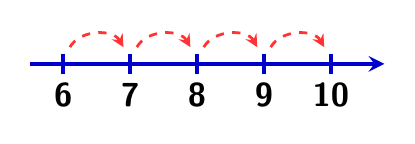
\begin{tikzpicture}[scale=0.85, baseline=(current bounding box.center)]
  \draw[->, >=stealth, line width=1.5pt, blue!80!black] (5.5,0) -- (10.8,0);
  \foreach \x in {6,7,8,9,10} {
    \draw[line width=1.5pt, blue!80!black] (\x,0.15) -- (\x,-0.15);
    \node[font=\bfseries\large, below] at (\x,-0.15) {\x};
  }
  \foreach \x in {6,7,8,9} {
    \draw[->, >=stealth, dashed, line width=1pt, red!80] (\x+0.1,0.25) to[out=60,in=120] (\x+0.9,0.25);
  }
\end{tikzpicture}
\end{center}
Xét tính đúng sai của các câu sau:
\choiceTF
{\True Số $10$ là số bé nhất có hai chữ số.}
{\True Số liền trước của số $8$ là số $7$.}
{Số liền sau của số $9$ là số $8$.}
{\True Số liền sau của số $9$ là số $10$.}
\loigiai{
\begin{itemize}
    \item Số $10$ là số bé nhất có hai chữ số: \textbf{Đúng}.
    \item Số $7$ đứng trước số $8$: \textbf{Đúng}.
    \item Số liền sau của số $9$ phải là $10$ (không phải $8$): \textbf{Sai}.
    \item Số liền sau của số $9$ là số $10$: \textbf{Đúng}.
\end{itemize}
}
\end{ex}

% --- CÂU 14 ---
\begin{ex} %[1D1V02]
Quan sát thứ tự dãy số từ $6$ đến $10$:
\begin{center}
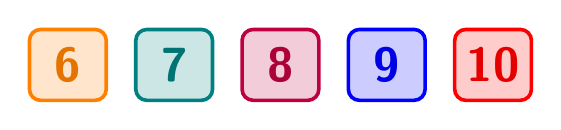
\begin{tikzpicture}[scale=0.75, baseline=(current bounding box.center)]
  \foreach \i/\num/\c in {0/6/orange, 1/7/teal, 2/8/purple, 3/9/blue, 4/10/red} {
    \draw[fill=\c!20, draw=\c, line width=1.3pt, rounded corners=4pt] (\i*1.8,-0.4) rectangle (\i*1.8+1.3,0.8);
    \node[font=\LARGE\bfseries, text=\c!90!black] at (\i*1.8+0.65, 0.2) {\num};
  }
\end{tikzpicture}
\end{center}
Xét tính đúng sai của các câu sau:
\choiceTF
{\True Dãy số được sắp xếp theo thứ tự tăng dần.}
{\True Số đứng đầu dãy là $6$, số đứng cuối dãy là $10$.}
{Số $8$ đứng liền sau số $9$.}
{\True Số $8$ đứng liền trước số $9$.}
\loigiai{
\begin{itemize}
    \item Dãy số tăng dần: \textbf{Đúng}.
    \item Đầu dãy là $6$, cuối dãy là $10$: \textbf{Đúng}.
    \item Số $8$ đứng trước số $9$: \textbf{Sai} (câu c bảo đứng sau).
    \item Số $8$ đứng liền trước số $9$: \textbf{Đúng}.
\end{itemize}
}
\end{ex}

% =========================================================================
% PHẦN 3: TRẢ LỜI NGẮN (ĐIỀN SỐ THÍCH HỢP VÀO Ô TRỐNG)
% =========================================================================
\textbf{Phần 3. Trả lời ngắn (Quan sát hình vẽ và điền số thích hợp)}
\setcounterpageref{ex}{0}

% --- CÂU 15 ---
\begin{ex} %[1D1H02]
Đếm tổng số ngón tay trên cả hai bàn tay dưới đây:
\begin{center}
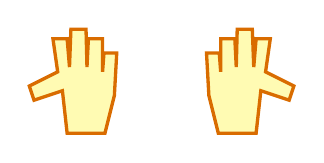
\begin{tikzpicture}[scale=0.6, baseline=(current bounding box.center)]
  \begin{scope}[shift={(-2,0)}]
    \draw[fill=yellow!30, draw=orange!85!black, line width=1.2pt]
      (0,-0.5) -- (-0.1,0.4) -- (-0.7,0.2) -- (-0.8,0.5) -- (-0.2,0.8)
      -- (-0.3,1.5) -- (0,1.5) -- (0.05,0.9)
      -- (0.08,1.7) -- (0.4,1.7) -- (0.42,0.9)
      -- (0.45,1.5) -- (0.75,1.5) -- (0.75,0.8)
      -- (0.78,1.2) -- (1.05,1.2) -- (1.0,0.3)
      -- (0.8,-0.5) -- cycle;
  \end{scope}
  \begin{scope}[shift={(2,0)}, xscale=-1]
    \draw[fill=yellow!30, draw=orange!85!black, line width=1.2pt]
      (0,-0.5) -- (-0.1,0.4) -- (-0.7,0.2) -- (-0.8,0.5) -- (-0.2,0.8)
      -- (-0.3,1.5) -- (0,1.5) -- (0.05,0.9)
      -- (0.08,1.7) -- (0.4,1.7) -- (0.42,0.9)
      -- (0.45,1.5) -- (0.75,1.5) -- (0.75,0.8)
      -- (0.78,1.2) -- (1.05,1.2) -- (1.0,0.3)
      -- (0.8,-0.5) -- cycle;
  \end{scope}
\end{tikzpicture}
\end{center}
\shortans{10}
\loigiai{
\textbf{Đáp số:} $10$\\
Hai bàn tay có tất cả $10$ ngón tay.
}
\end{ex}

% --- CÂU 16 ---
\begin{ex} %[1D1H02]
Điền số liền sau của số $7$ vào ô trống còn thiếu:
\begin{center}
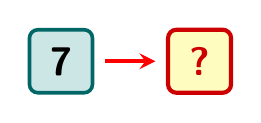
\begin{tikzpicture}[scale=0.8, baseline=(current bounding box.center)]
  \draw[fill=teal!20, draw=teal!80!black, line width=1.3pt, rounded corners=3pt] (-1.2,-0.4) rectangle (-0.2,0.6);
  \node[font=\Large\bfseries] at (-0.7,0.1) {7};
  \draw[->, >=stealth, line width=1.5pt, red] (0,0.1) -- (0.8,0.1);
  \draw[fill=yellow!25, draw=red!80!black, line width=1.5pt, rounded corners=3pt] (1.0,-0.4) rectangle (2.0,0.6);
  \node[font=\Large\bfseries, text=red!80!black] at (1.5,0.1) {?};
\end{tikzpicture}
\end{center}
\shortans{8}
\loigiai{
\textbf{Đáp số:} $8$\\
Số liền sau của số $7$ là số $8$.
}
\end{ex}

% --- CÂU 17 ---
\begin{ex} %[1D1V02]
Điền số liền trước của số $10$ vào ô trống còn thiếu:
\begin{center}
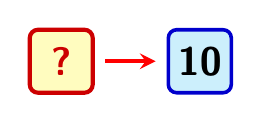
\begin{tikzpicture}[scale=0.8, baseline=(current bounding box.center)]
  \draw[fill=yellow!25, draw=red!80!black, line width=1.5pt, rounded corners=3pt] (-1.5,-0.4) rectangle (-0.5,0.6);
  \node[font=\Large\bfseries, text=red!80!black] at (-1.0,0.1) {?};
  \draw[->, >=stealth, line width=1.5pt, red] (-0.3,0.1) -- (0.5,0.1);
  \draw[fill=cyan!20, draw=blue!80!black, line width=1.3pt, rounded corners=3pt] (0.7,-0.4) rectangle (1.7,0.6);
  \node[font=\Large\bfseries] at (1.2,0.1) {10};
\end{tikzpicture}
\end{center}
\shortans{9}
\loigiai{
\textbf{Đáp số:} $9$\\
Số liền trước của số $10$ là số $9$.
}
\end{ex}

% --- CÂU 18 ---
\begin{ex} %[1D1V02]
Số nào đứng ở giữa số $6$ và số $8$?
\begin{center}
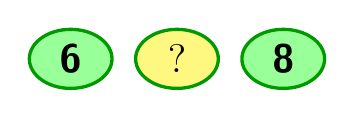
\begin{tikzpicture}[scale=0.75, baseline=(current bounding box.center)]
  \foreach \x/\num/\c in {-1.8/6/green!40, 0/{$\mathbf{?}$}/yellow!50, 1.8/8/green!40} {
    \draw[fill=\c, draw=green!60!black, line width=1.2pt] (\x,0) ellipse (0.7cm and 0.5cm);
    \node[font=\Large\bfseries] at (\x,0) {\num};
  }
\end{tikzpicture}
\end{center}
\shortans{7}
\loigiai{
\textbf{Đáp số:} $7$\\
Số đứng giữa $6$ và $8$ là số $7$.
}
\end{ex}

% --- CÂU 19 ---
\begin{ex} %[1D1V02]
Trong bể có $5$ con cá vàng, thả thêm $4$ con cá xanh. Hỏi trong bể có tất cả bao nhiêu con cá?
\begin{center}
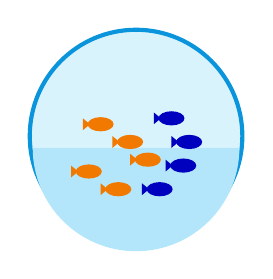
\begin{tikzpicture}[scale=0.75, baseline=(current bounding box.center)]
  \draw[fill=cyan!15, draw=cyan!80!blue, line width=1.5pt] (0,0) circle (1.8cm);
  \fill[cyan!30] (-1.75,-0.2) arc (180:360:1.75cm) -- cycle;
  % 5 cá vàng
  \foreach \px/\py in {-0.8/-0.6, -0.3/-0.9, -0.6/0.2, 0.2/-0.4, -0.1/-0.1} {
    \fill[orange!95!black] (\px,\py) ellipse (0.22cm and 0.12cm);
    \fill[orange!95!black] (\px-0.18,\py) -- (\px-0.3,\py+0.1) -- (\px-0.3,\py-0.1) -- cycle;
  }
  % 4 cá xanh
  \foreach \px/\py in {0.6/0.3, 0.8/-0.5, 0.4/-0.9, 0.9/-0.1} {
    \fill[blue!75!black] (\px,\py) ellipse (0.22cm and 0.12cm);
    \fill[blue!75!black] (\px-0.18,\py) -- (\px-0.3,\py+0.1) -- (\px-0.3,\py-0.1) -- cycle;
  }
\end{tikzpicture}
\end{center}
\shortans{9}
\loigiai{
\textbf{Đáp số:} $9$\\
Trong bể có tất cả $5 + 4 = 9$ con cá.
}
\end{ex}

% --- CÂU 20 ---
\begin{ex} %[1D1C02]
Đếm số ngôi sao mang số có \textbf{một chữ số lớn hơn 5} dưới đây:
\begin{center}
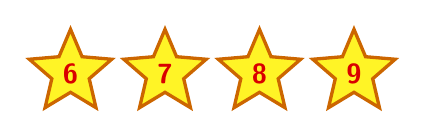
\begin{tikzpicture}[scale=0.75, baseline=(current bounding box.center)]
  \foreach \i/\num in {0/6, 1/7, 2/8, 3/9} {
    \node[draw=orange!80!black, fill=yellow!85, star, star points=5, star point ratio=2.2, line width=1.2pt, minimum size=1.1cm] at (\i*1.6,0) {};
    \node[font=\bfseries\normalsize, text=red!85!black] at (\i*1.6,-0.02) {\num};
  }
\end{tikzpicture}
\end{center}
\shortans{4}
\loigiai{
\textbf{Đáp số:} $4$\\
Có $4$ số có một chữ số lớn hơn $5$ là: $6, 7, 8, 9$.
}
\end{ex}

\newpage

\subsection*{Bài 03. Nhiều hơn, ít hơn, bằng nhau}
\addcontentsline{toc}{subsection}{Bài 03. Nhiều hơn, ít hơn, bằng nhau}
\TaoPhieuKiemTra{Chủ đề 1 -- Các số từ 0 đến 10}{03}{Nhiều hơn, ít hơn, bằng nhau}{https://loptoanthaylinh.vn/thi-online/toan-1/bai-03}
% =========================================================================
% BÀI 03: NHIỀU HƠN, ÍT HƠN, BẰNG NHAU (CHỦ ĐỀ 1 - LỚP 1)
% TOÀN BỘ CÂU HỎI ĐƯỢC VẼ HÌNH MINH HỌA TRỰC QUAN 100% BẰNG TIKZ
% =========================================================================

% --- CÁC HÀM VẼ ĐỒ VẬT, CON VẬT TRỰC QUAN CHO HỌC SINH LỚP 1 ---
\newcommand{\VeBanNho}[3][blue!70]{% #1=màu áo, #2=x, #3=y
  \begin{scope}[shift={(#2,#3)}, scale=0.62]
    \fill[orange!22] (0, 0.55) circle (0.24cm);
    \fill[brown!80!black] (-0.24,0.6) arc (180:0:0.24cm) -- cycle;
    \fill[black] (-0.08,0.56) circle (0.03cm);
    \fill[black] (0.08,0.56) circle (0.03cm);
    \draw[line width=0.6pt, red!70!black] (-0.06,0.48) arc (-150:-30:0.08cm);
    \fill[#1] (-0.18,0.1) rectangle (0.18,0.38);
    \draw[line width=1.4pt, blue!90!black] (-0.09,0.1) -- (-0.09,-0.15);
    \draw[line width=1.4pt, blue!90!black] (0.09,0.1) -- (0.09,-0.15);
  \end{scope}
}

\newcommand{\VeQuaTao}[2]{% #1=x, #2=y
  \begin{scope}[shift={(#1,#2)}, scale=0.65]
    \fill[red!85!black] (-0.11,0.08) circle (0.22cm);
    \fill[red!85!black] (0.11,0.08) circle (0.22cm);
    \fill[red!85!black] (0,-0.05) circle (0.24cm);
    \draw[line width=1pt, brown!80!black] (0,0.24) to[out=70,in=-110] (0.06,0.42);
    \fill[green!70!black] (0.05,0.36) to[out=20,in=160] (0.24,0.42) to[out=-120,in=-20] cycle;
  \end{scope}
}

\newcommand{\VeQuaLe}[2]{% #1=x, #2=y
  \begin{scope}[shift={(#1,#2)}, scale=0.65]
    \fill[lime!75!black] (0,0.12) circle (0.16cm);
    \fill[lime!75!black] (0,-0.08) circle (0.24cm);
    \draw[line width=1pt, brown!80!black] (0,0.26) to[out=70,in=-110] (0.06,0.42);
    \fill[green!70!black] (0.05,0.36) to[out=20,in=160] (0.22,0.4) to[out=-120,in=-20] cycle;
  \end{scope}
}

\newcommand{\VeChiecO}[3][cyan!70!blue]{% #1=màu dù, #2=x, #3=y
  \begin{scope}[shift={(#2,#3)}, scale=0.68]
    \fill[#1] (-0.45,0.15) arc (180:0:0.45cm) -- cycle;
    \draw[line width=1.1pt, gray!80!black] (0,0.58) -- (0,-0.18) arc (0:-180:0.09cm);
    \fill[gray!80!black] (-0.03,0.58) rectangle (0.03,0.65);
  \end{scope}
}

\newcommand{\VeBongHoa}[3][magenta!80!red]{% #1=màu cánh, #2=x, #3=y
  \begin{scope}[shift={(#2,#3)}, scale=0.65]
    \draw[line width=1.1pt, green!60!black] (0,0) -- (0,-0.4);
    \fill[green!60!black] (0,-0.22) to[out=30,in=150] (0.18,-0.2) to[out=-120,in=-30] cycle;
    \foreach \a in {0,72,144,216,288} {
      \fill[#1] (\a:0.16) circle (0.1cm);
    }
    \fill[yellow!90!orange] (0,0) circle (0.08cm);
  \end{scope}
}

\newcommand{\VeChuChim}[2]{% #1=x, #2=y
  \begin{scope}[shift={(#1,#2)}, scale=0.55]
    \fill[cyan!80!blue] (0,0.2) circle (0.26cm);
    \fill[cyan!60!black] (-0.1,0.18) ellipse (0.16cm and 0.1cm);
    \fill[cyan!80!blue] (0.16,0.38) circle (0.17cm);
    \fill[white] (0.22,0.42) circle (0.05cm);
    \fill[black] (0.23,0.42) circle (0.03cm);
    \fill[orange!95!black] (0.32,0.38) -- (0.24,0.34) -- (0.24,0.42) -- cycle;
    \draw[line width=1pt, orange!90!black] (-0.06,-0.05) -- (-0.06,-0.2);
    \draw[line width=1pt, orange!90!black] (0.06,-0.05) -- (0.06,-0.2);
  \end{scope}
}

\newcommand{\VeChiecMu}[3][red!80!black]{% #1=màu mũ, #2=x, #3=y
  \begin{scope}[shift={(#2,#3)}, scale=0.65]
    \fill[#1] (-0.28,0) arc (180:0:0.28cm) -- cycle;
    \draw[line width=1.8pt, #1] (-0.38,0) -- (0.38,0);
  \end{scope}
}

\newcommand{\VeChuMeo}[2]{% #1=x, #2=y
  \begin{scope}[shift={(#1,#2)}, scale=0.62]
    \fill[orange!85!black] (0,0.18) circle (0.26cm);
    \fill[orange!85!black] (-0.22,0.32) -- (-0.12,0.54) -- (-0.02,0.4) -- cycle;
    \fill[pink!70] (-0.19,0.34) -- (-0.12,0.48) -- (-0.05,0.39) -- cycle;
    \fill[orange!85!black] (0.22,0.32) -- (0.12,0.54) -- (0.02,0.4) -- cycle;
    \fill[pink!70] (0.19,0.34) -- (0.12,0.48) -- (0.05,0.39) -- cycle;
    \fill[black] (-0.09,0.22) circle (0.032cm);
    \fill[black] (0.09,0.22) circle (0.032cm);
    \fill[pink!80!black] (0,0.14) circle (0.028cm);
    \draw[line width=0.5pt, gray!70!black] (-0.07,0.14) -- (-0.24,0.16);
    \draw[line width=0.5pt, gray!70!black] (-0.07,0.12) -- (-0.24,0.1);
    \draw[line width=0.5pt, gray!70!black] (0.07,0.14) -- (0.24,0.16);
    \draw[line width=0.5pt, gray!70!black] (0.07,0.12) -- (0.24,0.1);
  \end{scope}
}

\newcommand{\VeConCa}[2]{% #1=x, #2=y
  \begin{scope}[shift={(#1,#2)}, scale=0.65]
    \fill[cyan!75!blue] (0,0) ellipse (0.3cm and 0.17cm);
    \fill[cyan!75!blue] (-0.26,0) -- (-0.42,0.15) -- (-0.42,-0.15) -- cycle;
    \fill[white] (0.13,0.05) circle (0.045cm);
    \fill[black] (0.15,0.05) circle (0.025cm);
  \end{scope}
}

\newcommand{\VeChiecGhe}[2]{% #1=x, #2=y
  \begin{scope}[shift={(#1,#2)}, scale=0.62]
    \draw[line width=1.4pt, brown!80!black] (-0.24,-0.38) -- (-0.24,0.42);
    \draw[line width=1.4pt, brown!80!black] (0.24,-0.38) -- (0.24,0);
    \draw[line width=2.4pt, brown!80!black] (-0.28,0) -- (0.28,0);
    \draw[line width=1.3pt, brown!80!black] (-0.24,0.14) -- (0.24,0.14);
    \draw[line width=1.3pt, brown!80!black] (-0.24,0.32) -- (0.24,0.32);
  \end{scope}
}

\newcommand{\VeDauTay}[2]{% #1=x, #2=y
  \begin{scope}[shift={(#1,#2)}, scale=0.62]
    \fill[red!85!black] (-0.2,0.08) .. controls (-0.2,-0.18) and (-0.05,-0.32) .. (0,-0.36) .. controls (0.05,-0.32) and (0.2,-0.18) .. (0.2,0.08) -- cycle;
    \fill[green!70!black] (-0.18,0.08) -- (0,0.2) -- (0.18,0.08) -- (0,0.12) -- cycle;
    \fill[yellow!90!black] (-0.07,-0.04) circle (0.02cm);
    \fill[yellow!90!black] (0.07,-0.04) circle (0.02cm);
    \fill[yellow!90!black] (0,-0.18) circle (0.02cm);
  \end{scope}
}

\newcommand{\VeCocNuoc}[2]{% #1=x, #2=y
  \begin{scope}[shift={(#1,#2)}, scale=0.62]
    \draw[line width=1.2pt, cyan!70!blue] (-0.2,0.28) -- (-0.14,-0.22) -- (0.14,-0.22) -- (0.2,0.28);
    \fill[cyan!30] (-0.18,0.14) -- (-0.14,-0.2) -- (0.14,-0.2) -- (0.18,0.14) -- cycle;
  \end{scope}
}

\newcommand{\VeChiecThia}[2]{% #1=x, #2=y
  \begin{scope}[shift={(#1,#2)}, scale=0.62]
    \fill[gray!50] (0,0.18) ellipse (0.13cm and 0.2cm);
    \draw[line width=1.6pt, gray!70] (0,0.05) -- (0,-0.32);
  \end{scope}
}

\newcommand{\VeChuOng}[2]{% #1=x, #2=y
  \begin{scope}[shift={(#1,#2)}, scale=0.62]
    \fill[yellow!90!orange] (0,0) ellipse (0.22cm and 0.15cm);
    \draw[line width=1.1pt, black] (-0.06,-0.14) -- (-0.06,0.14);
    \draw[line width=1.1pt, black] (0.06,-0.14) -- (0.06,0.14);
    \fill[cyan!20, draw=cyan!70!black, line width=0.4pt] (-0.05,0.1) ellipse (0.11cm and 0.16cm);
    \fill[cyan!20, draw=cyan!70!black, line width=0.4pt] (0.05,0.1) ellipse (0.11cm and 0.16cm);
    \fill[black] (0.16,0.04) circle (0.025cm);
  \end{scope}
}

\newcommand{\VeChuBuom}[2]{% #1=x, #2=y
  \begin{scope}[shift={(#1,#2)}, scale=0.62]
    \fill[purple!70!blue] (-0.16,0.12) ellipse (0.18cm and 0.12cm);
    \fill[purple!70!blue] (0.16,0.12) ellipse (0.18cm and 0.12cm);
    \fill[purple!60!pink] (-0.14,-0.08) ellipse (0.14cm and 0.09cm);
    \fill[purple!60!pink] (0.14,-0.08) ellipse (0.14cm and 0.09cm);
    \fill[black] (0,0) ellipse (0.04cm and 0.2cm);
    \draw[line width=0.6pt, black] (0,0.18) to[out=60,in=-60] (0.08,0.32);
    \draw[line width=0.6pt, black] (0,0.18) to[out=120,in=-120] (-0.08,0.32);
  \end{scope}
}

% =========================================================================
% PHẦN 1: TRẮC NGHIỆM LỰA CHỌN (12 CÂU)
% =========================================================================
\textbf{Phần 1. Trắc nghiệm lựa chọn (Học sinh quan sát hình và chọn đáp án đúng)}
\setcounterpageref{ex}{0}

% --- CÂU 1 ---
\begin{ex} %[1D1N03]
Quan sát hàng thỏ và hàng củ cà rốt dưới đây. Em thấy số thỏ và số cà rốt như thế nào?
\begin{center}
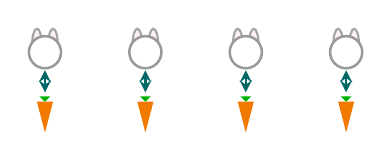
\begin{tikzpicture}[scale=0.85, baseline=(current bounding box.center)]
  \foreach \x in {-2.25, -0.75, 0.75, 2.25} {
    \draw[fill=pink!20, draw=gray!70, line width=0.8pt] (\x-0.12, 0.45) ellipse (0.07cm and 0.22cm);
    \draw[fill=pink!20, draw=gray!70, line width=0.8pt] (\x+0.12, 0.45) ellipse (0.07cm and 0.22cm);
    \draw[fill=white, draw=gray!80, line width=0.9pt] (\x, 0.32) circle (0.24cm);
    \draw[<->, >=stealth, dashed, line width=0.9pt, teal!80!black] (\x, 0.05) -- (\x, -0.28);
    \fill[orange!95!black] (\x-0.12, -0.42) -- (\x+0.12, -0.42) -- (\x, -0.88) -- cycle;
    \fill[green!70!black] (\x, -0.42) -- (\x-0.08, -0.34) -- (\x+0.08, -0.34) -- cycle;
  }
\end{tikzpicture}
\end{center}
\choice
{\True Bằng nhau}
{Thỏ nhiều hơn cà rốt}
{Thỏ ít hơn cà rốt}
{Không so sánh được}
\loigiai{
Mỗi chú thỏ được nối tương ứng với một củ cà rốt. Cả hai hàng đều có $4$ hình ($4 = 4$).\\
Vậy số thỏ và số cà rốt \textbf{bằng nhau}.\\
\textbf{Đáp án của câu hỏi là A}
}
\end{ex}

% --- CÂU 2 ---
\begin{ex} %[1D1N03]
Quan sát hình vẽ bông hoa và chú bướm dưới đây. Khẳng định nào sau đây đúng?
\begin{center}
\begin{tikzpicture}[scale=0.8, baseline=(current bounding box.center)]
  \foreach \x in {-1.8, 0, 1.8} {
    \VeChuBuom{\x}{0.6}
    \draw[->, >=stealth, dashed, line width=0.9pt, red!70!black] (\x, 0.3) -- (\x, -0.15);
  }
  \foreach \x in {-1.8, -0.9, 0, 0.9, 1.8} {
    \VeBongHoa{\x}{-0.45}
  }
\end{tikzpicture}
\end{center}
\choice
{Số hoa ít hơn số bướm}
{Số hoa bằng số bướm}
{\True Số hoa nhiều hơn số bướm}
{Số bướm nhiều hơn số hoa}
\loigiai{
Có 3 chú bướm và 5 bông hoa. Vì $5 > 3$ nên \textbf{số hoa nhiều hơn số bướm}.\\
\textbf{Đáp án của câu hỏi là C}
}
\end{ex}

% --- CÂU 3 ---
\begin{ex} %[1D1H03]
Quan sát hình vẽ chiếc chén và chiếc đĩa dưới đây:
\begin{center}
\begin{tabular}{cc}
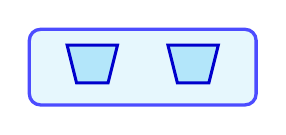
\begin{tikzpicture}[scale=0.8]
  \draw[fill=cyan!10, draw=blue!70, line width=1.2pt, rounded corners=4pt] (-1.8,-0.5) rectangle (1.8,0.7);
  \foreach \x in {-0.8, 0.8} {
    \draw[fill=cyan!30, draw=blue!80!black, line width=1.1pt] (\x-0.4, 0.45) -- (\x+0.4, 0.45) -- (\x+0.25, -0.15) -- (\x-0.25, -0.15) -- cycle;
  }
\end{tikzpicture}
&
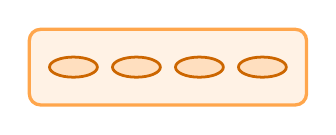
\begin{tikzpicture}[scale=0.8]
  \draw[fill=orange!10, draw=orange!70, line width=1.2pt, rounded corners=4pt] (-2.2,-0.5) rectangle (2.2,0.7);
  \foreach \x in {-1.5, -0.5, 0.5, 1.5} {
    \draw[fill=orange!25, draw=orange!80!black, line width=1pt] (\x, 0.1) ellipse (0.38cm and 0.16cm);
  }
\end{tikzpicture} \\[4pt]
{\bfseries\color{blue!90!black} 2 chiếc chén} & {\bfseries\color{orange!90!black} 4 chiếc đĩa}
\end{tabular}
\end{center}
Khẳng định nào sau đây đúng?
\choice
{Số chén nhiều hơn số đĩa}
{Số chén bằng số đĩa}
{Số đĩa ít hơn số chén}
{\True Số chén ít hơn số đĩa}
\loigiai{
Có 2 chiếc chén và 4 chiếc đĩa. Vì $2 < 4$ nên \textbf{số chén ít hơn số đĩa}.\\
\textbf{Đáp án của câu hỏi là D}
}
\end{ex}

% --- CÂU 4 ---
\begin{ex} %[1D1H03]
Hai tổ xếp thành hai hàng thẳng nhau như hình dưới đây:
\begin{center}
\begin{tikzpicture}[scale=0.85, baseline=(current bounding box.center)]
  \node[font=\bfseries\color{blue!80!black}, anchor=east] at (-2.4, 0.38) {Tổ Một (5 bạn):};
  \node[font=\bfseries\color{red!80!black}, anchor=east] at (-2.4, -0.42) {Tổ Hai (5 bạn):};
  \foreach \x in {-1.6, -0.8, 0, 0.8, 1.6} {
    \VeBanNho[blue!70]{\x}{0.35}
    \draw[<->, >=stealth, dashed, line width=0.8pt, gray!80] (\x, 0.1) -- (\x, -0.15);
    \VeBanNho[orange!85!black]{\x}{-0.4}
  }
\end{tikzpicture}
\end{center}
Số bạn của hai tổ là
\choice
{Tổ Một nhiều hơn}
{\True Bằng nhau}
{Tổ Hai nhiều hơn}
{Không biết}
\loigiai{
Mỗi bạn tổ Một đối diện với đúng một bạn tổ Hai, hai tổ đều có 5 bạn ($5 = 5$).\\
Vậy số bạn của hai tổ \textbf{bằng nhau}.\\
\textbf{Đáp án của câu hỏi là B}
}
\end{ex}

\newpage
% --- CÂU 5 ---
\begin{ex} %[1D1H03]
Quan sát ngôi sao ở Hình A và Hình B:
\begin{center}
\begin{tabular}{cc}

\begin{tikzpicture}[scale=0.8]
  \draw[fill=yellow!10, draw=orange!80, line width=1.2pt, rounded corners=4pt] (-1.8,-0.6) rectangle (1.8,0.6);
  \foreach \x/\y in {-1.1/0.25, 0/0.25, 1.1/0.25, -1.1/-0.25, 0/-0.25, 1.1/-0.25} {
    \node[draw=orange!80!black, fill=yellow!80, star, star points=5, star point ratio=2.2, line width=0.7pt, minimum size=0.55cm] at (\x,\y) {};
  }
\end{tikzpicture}
&

\begin{tikzpicture}[scale=0.8]
  \draw[fill=cyan!10, draw=blue!80, line width=1.2pt, rounded corners=4pt] (-1.5,-0.6) rectangle (1.5,0.6);
  \foreach \x/\y in {-0.7/0.25, 0.7/0.25, -0.7/-0.25, 0.7/-0.25} {
    \node[draw=blue!80!black, fill=cyan!60, star, star points=5, star point ratio=2.2, line width=0.7pt, minimum size=0.55cm] at (\x,\y) {};
  }
\end{tikzpicture} \\[4pt]
{\bfseries\color{orange!90!black} Hình A (6 ngôi sao)} & {\bfseries\color{blue!90!black} Hình B (4 ngôi sao)}
\end{tabular}
\end{center}
Khẳng định nào sau đây đúng?
\choice
{Hình A ít hơn hình B}
{Hình A bằng hình B}
{\True Hình A nhiều hơn hình B}
{Hình B nhiều hơn hình A}
\loigiai{
Hình A có 6 ngôi sao, Hình B có 4 ngôi sao. Vì $6 > 4$ nên \textbf{Hình A nhiều hơn hình B}.\\
\textbf{Đáp án của câu hỏi là C}
}
\end{ex}

% --- CÂU 6 ---
\begin{ex} %[1D1H03]
Quan sát số chú chim và số chiếc lồng chim:
\begin{center}
\begin{tikzpicture}[scale=0.85, baseline=(current bounding box.center)]
  \node[font=\bfseries\color{blue!80!black}, anchor=east] at (-2.3, 0.4) {3 chú chim:};
  \foreach \x in {-1.4, 0, 1.4} {
    \VeChuChim{\x}{0.35}
  }
  \node[font=\bfseries\color{brown!80!black}, anchor=east] at (-2.3, -0.45) {5 lồng chim:};
  \foreach \x in {-1.8, -0.9, 0, 0.9, 1.8} {
    \draw[fill=yellow!15, draw=brown!80!black, line width=1pt, rounded corners=2pt] (\x-0.3, -0.7) rectangle (\x+0.3, -0.2);
    \draw[brown!80!black, line width=0.6pt] (\x-0.1, -0.7) -- (\x-0.1, -0.2);
    \draw[brown!80!black, line width=0.6pt] (\x+0.1, -0.7) -- (\x+0.1, -0.2);
  }
\end{tikzpicture}
\end{center}
Khẳng định nào sau đây đúng?
\choice
{Số chim nhiều hơn số lồng}
{Số chim bằng số lồng}
{\True Số chim ít hơn số lồng}
{Số lồng ít hơn số chim}
\loigiai{
Có 3 chú chim và 5 lồng chim. Vì $3 < 5$ nên \textbf{số chim ít hơn số lồng}.\\
\textbf{Đáp án của câu hỏi là C}
}
\end{ex}

% --- CÂU 7 ---
\begin{ex} %[1D1H03]
Có 5 bạn nhỏ và 4 chiếc mũ. Mỗi bạn đội một chiếc mũ thì:
\begin{center}
\begin{tikzpicture}[scale=0.85, baseline=(current bounding box.center)]
  \node[font=\bfseries, anchor=east] at (-2.4, 0.4) {5 bạn nhỏ:};
  \foreach \x in {-1.6, -0.8, 0, 0.8, 1.6} {
    \VeBanNho[teal!80!black]{\x}{0.35}
  }
  \node[font=\bfseries, anchor=east] at (-2.4, -0.4) {4 chiếc mũ:};
  \foreach \x in {-1.6, -0.8, 0, 0.8} {
    \draw[<->, >=stealth, dashed, line width=0.8pt, gray] (\x, 0.08) -- (\x, -0.2);
    \VeChiecMu[red!85!black]{\x}{-0.35}
  }
  \node[font=\bfseries\Large\color{red!80!black}] at (1.6, -0.35) {?};
\end{tikzpicture}
\end{center}
\choice
{Đủ mũ cho các bạn}
{Thừa 1 chiếc mũ}
{Thừa 2 chiếc mũ}
{\True Thiếu 1 chiếc mũ}
\loigiai{
Có 5 bạn nhỏ mà chỉ có 4 chiếc mũ. Mỗi bạn một mũ thì còn 1 bạn chưa có mũ.\\
Vậy \textbf{thiếu 1 chiếc mũ}.\\
\textbf{Đáp án của câu hỏi là D}
}
\end{ex}

% --- CÂU 8 ---
\begin{ex} %[1D1V03]
Quan sát đĩa táo và đĩa lê dưới đây:
\begin{center}
\begin{tabular}{cc}
\begin{tikzpicture}[scale=0.8]
  \draw[fill=red!8, draw=red!70, line width=1.2pt, rounded corners=4pt] (-2.2,-0.5) rectangle (2.2,0.6);
  \foreach \x in {-1.8, -1.2, -0.6, 0, 0.6, 1.2, 1.8} {
    \VeQuaTao{\x}{0.05}
  }
\end{tikzpicture}
&
\begin{tikzpicture}[scale=0.8]
  \draw[fill=green!8, draw=green!70!black, line width=1.2pt, rounded corners=4pt] (-1.8,-0.5) rectangle (1.8,0.6);
  \foreach \x in {-1.2, -0.6, 0, 0.6, 1.2} {
    \VeQuaLe{\x}{0.05}
  }
\end{tikzpicture} \\[4pt]
{\bfseries\color{red!85!black} Đĩa A (7 quả táo)} & {\bfseries\color{green!70!black} Đĩa B (5 quả lê)}
\end{tabular}
\end{center}
Khẳng định nào sau đây đúng?
\choice
{Số quả lê nhiều hơn số quả táo}
{Số táo bằng số lê}
{Số quả táo ít hơn số quả lê}
{\True Số quả táo nhiều hơn số quả lê}
\loigiai{
Đĩa A có 7 quả táo, Đĩa B có 5 quả lê. Vì $7 > 5$ nên \textbf{số quả táo nhiều hơn số quả lê}.\\
\textbf{Đáp án của câu hỏi là D}
}
\end{ex}

\newpage
% --- CÂU 9 ---
\begin{ex} %[1D1V03]
Quan sát hai bình cá:
\begin{center}
\begin{tabular}{cc}
\begin{tikzpicture}[scale=0.75]
  \draw[fill=cyan!15, draw=blue!70, line width=1.3pt] (0,0) circle (1.2cm);
  \fill[cyan!30] (-1.15,-0.1) arc (180:360:1.15cm) -- cycle;
  \VeConCa{-0.3}{-0.4}
  \VeConCa{0.3}{-0.6}
  \VeConCa{0.0}{0.2}
\end{tikzpicture}
&
\begin{tikzpicture}[scale=0.75]
  \draw[fill=cyan!15, draw=blue!70, line width=1.3pt] (0,0) circle (1.2cm);
  \fill[cyan!30] (-1.15,-0.1) arc (180:360:1.15cm) -- cycle;
  \VeConCa{-0.3}{-0.5}
  \VeConCa{0.3}{-0.3}
  \VeConCa{0.0}{0.2}
\end{tikzpicture} \\[4pt]
{\bfseries\color{blue!90!black} Bình A (3 chú cá)} & {\bfseries\color{blue!90!black} Bình B (3 chú cá)}
\end{tabular}
\end{center}
Khẳng định nào đúng?
\choice
{\True Số cá ở hai bình bằng nhau}
{Bình A nhiều hơn bình B}
{Bình B nhiều hơn bình A}
{Không so sánh được}
\loigiai{
Cả hai bình đều có 3 chú cá ($3 = 3$).\\
Vậy \textbf{số cá ở hai bình bằng nhau}.\\
\textbf{Đáp án của câu hỏi là A}
}
\end{ex}

% --- CÂU 10 ---
\begin{ex} %[1D1V03]
Khung nào dưới đây có nhiều chấm tròn hơn?
\begin{center}
\begin{tabular}{cc}
\begin{tikzpicture}[scale=0.8]
  \draw[fill=orange!10, draw=orange!80, line width=1.2pt, rounded corners=4pt] (-1.8,-0.7) rectangle (1.8,0.7);
  \foreach \x/\y in {-1.2/0.35, -0.4/0.35, 0.4/0.35, 1.2/0.35, -1.2/-0.35, -0.4/-0.35, 0.4/-0.35, 1.2/-0.35} {
    \fill[orange!95!black] (\x,\y) circle (0.16cm);
  }
\end{tikzpicture}
&
\begin{tikzpicture}[scale=0.8]
  \draw[fill=teal!10, draw=teal!80, line width=1.2pt, rounded corners=4pt] (-1.5,-0.7) rectangle (1.5,0.7);
  \foreach \x/\y in {-0.8/0.35, 0/0.35, 0.8/0.35, -0.8/-0.35, 0/-0.35, 0.8/-0.35} {
    \fill[teal!90!black] (\x,\y) circle (0.16cm);
  }
\end{tikzpicture} \\[4pt]
{\bfseries\color{orange!90!black} Khung A (8 chấm)} & {\bfseries\color{teal!90!black} Khung B (6 chấm)}
\end{tabular}
\end{center}
\choice
{\True Khung A nhiều hơn}
{Khung B nhiều hơn}
{Hai khung bằng nhau}
{Khung A ít hơn}
\loigiai{
Khung A có 8 chấm tròn, Khung B có 6 chấm tròn. Vì $8 > 6$ nên \textbf{Khung A nhiều hơn}.\\
\textbf{Đáp án của câu hỏi là A}
}
\end{ex}

% --- CÂU 11 ---
\begin{ex} %[1D1V03]
Quan sát đĩa bánh đỏ và đĩa bánh xanh:
\begin{center}
\begin{tabular}{cc}
\begin{tikzpicture}[scale=0.8]
  \draw[fill=red!8, draw=red!70, line width=1.2pt, rounded corners=4pt] (-1.8,-0.45) rectangle (1.8,0.55);
  \foreach \x in {-1.2, -0.4, 0.4, 1.2} {
    \draw[fill=orange!25, draw=orange!80!black, line width=1pt, rounded corners=2pt] (\x-0.25,-0.2) rectangle (\x+0.25,0.3);
  }
\end{tikzpicture}
&
\begin{tikzpicture}[scale=0.8]
  \draw[fill=green!8, draw=green!70!black, line width=1.2pt, rounded corners=4pt] (-1.8,-0.45) rectangle (1.8,0.55);
  \foreach \x in {-1.3, -0.65, 0, 0.65, 1.3} {
    \draw[fill=orange!25, draw=orange!80!black, line width=1pt, rounded corners=2pt] (\x-0.2,-0.2) rectangle (\x+0.2,0.3);
  }
\end{tikzpicture} \\[4pt]
{\bfseries\color{red!85!black} Đĩa đỏ (4 cái bánh)} & {\bfseries\color{green!70!black} Đĩa xanh (5 cái bánh)}
\end{tabular}
\end{center}
\choice
{Đĩa đỏ nhiều hơn đĩa xanh}
{\True Đĩa đỏ ít hơn đĩa xanh}
{Hai đĩa bằng nhau}
{Đĩa xanh ít hơn đĩa đỏ}
\loigiai{
Đĩa đỏ có 4 cái bánh, Đĩa xanh có 5 cái bánh. Vì $4 < 5$ nên \textbf{đĩa đỏ ít hơn đĩa xanh}.\\
\textbf{Đáp án của câu hỏi là B}
}
\end{ex}

% --- CÂU 12 ---
\begin{ex} %[1D1C03]
Trong các nhóm đồ vật dưới đây, nhóm nào có số lượng \textbf{nhiều nhất}?
\choice
{Nhóm 3 quả bóng}
{\True Nhóm 6 bông hoa}
{Nhóm 4 cái bút}
{Nhóm 2 ngôi sao}
\loigiai{
So sánh các số lượng: $6 > 4 > 3 > 2$.\\
Nhóm có số lượng nhiều nhất là \textbf{nhóm 6 bông hoa}.\\
\textbf{Đáp án của câu hỏi là B}
}
\end{ex}

\newpage
% =========================================================================
% PHẦN 2: TRẮC NGHIỆM ĐÚNG SAI (QUAN SÁT TRANH MINH HỌA)
% =========================================================================
\textbf{Phần 2. Trắc nghiệm đúng sai (Quan sát đồ vật và xét tính đúng/sai)}
\setcounterpageref{ex}{0}

% --- CÂU 13 ---
\begin{ex} %[1D1H03]
Quan sát đồ vật chuẩn bị cho bữa tiệc sinh nhật:
\begin{center}
\begin{tabular}{cc}
\begin{tikzpicture}[scale=0.75]
  \draw[fill=blue!5, draw=blue!60, line width=1pt, rounded corners=4pt] (-2.2,-0.55) rectangle (2.2,0.55);
  \foreach \x in {-1.6, -0.8, 0, 0.8, 1.6} {
    \draw[fill=cyan!20, draw=blue!80, line width=0.9pt] (\x,0) ellipse (0.32cm and 0.16cm);
  }
  \node[font=\small\bfseries\color{blue!80!black}] at (0, -0.85) {5 chiếc đĩa};
\end{tikzpicture}
&
\begin{tikzpicture}[scale=0.75]
  \draw[fill=teal!5, draw=teal!60, line width=1pt, rounded corners=4pt] (-2.2,-0.55) rectangle (2.2,0.55);
  \foreach \x in {-1.6, -0.8, 0, 0.8, 1.6} {
    \VeChiecThia{\x}{0.05}
  }
  \node[font=\small\bfseries\color{teal!80!black}] at (0, -0.85) {5 chiếc thìa};
\end{tikzpicture} \\[16pt]
\begin{tikzpicture}[scale=0.75]
  \draw[fill=orange!5, draw=orange!60, line width=1pt, rounded corners=4pt] (-2.2,-0.55) rectangle (2.2,0.55);
  \foreach \x in {-1.1, 0, 1.1} {
    \VeCocNuoc{\x}{0.05}
  }
  \node[font=\small\bfseries\color{orange!90!black}] at (0, -0.85) {3 cốc nước};
\end{tikzpicture}
&
\begin{tikzpicture}[scale=0.75]
  \draw[fill=red!5, draw=red!60, line width=1pt, rounded corners=4pt] (-2.2,-0.55) rectangle (2.2,0.55);
  \foreach \x in {-1.6, -1.0, -0.3, 0.3, 1.0, 1.6} {
    \VeDauTay{\x}{0.05}
  }
  \node[font=\small\bfseries\color{red!80!black}] at (0, -0.85) {6 quả dâu tây};
\end{tikzpicture}
\end{tabular}
\end{center}
Xét tính đúng sai của các câu sau:
\choiceTF
{\True Số đĩa bằng số thìa}
{\True Số cốc nước ít hơn số đĩa}
{Số quả dâu ít hơn số cốc nước}
{\True Nhóm quả dâu tây có số lượng nhiều nhất}
\loigiai{
\begin{itemize}
    \item Số đĩa bằng số thìa ($5 = 5$): \textbf{Đúng}.
    \item Cốc nước (3) ít hơn đĩa (5): \textbf{Đúng}.
    \item Quả dâu (6) nhiều hơn cốc nước (3), nói ít hơn là: \textbf{Sai}.
    \item Quả dâu tây có 6 quả, là nhiều nhất: \textbf{Đúng}.
\end{itemize}
}
\end{ex}

% --- CÂU 14 ---
\begin{ex} %[1D1V03]
Quan sát vườn hoa xinh xắn:
\begin{center}
\begin{tabular}{ccc}
\begin{tikzpicture}[scale=0.75]
  \draw[fill=red!5, draw=red!60, line width=1pt, rounded corners=4pt] (-1.6,-0.55) rectangle (1.6,0.55);
  \foreach \x in {-1.05, -0.35, 0.35, 1.05} {
    \VeBongHoa{\x}{0.05}
  }
  \node[font=\small\bfseries\color{red!80!black}] at (0, -0.85) {4 bông hoa};
\end{tikzpicture}
&
\begin{tikzpicture}[scale=0.75]
  \draw[fill=yellow!10, draw=yellow!80!black, line width=1pt, rounded corners=4pt] (-1.6,-0.55) rectangle (1.6,0.55);
  \foreach \x in {-1.05, -0.35, 0.35, 1.05} {
    \VeChuOng{\x}{0.05}
  }
  \node[font=\small\bfseries\color{yellow!80!black}] at (0, -0.85) {4 chú ong};
\end{tikzpicture}
&
\begin{tikzpicture}[scale=0.75]
  \draw[fill=purple!5, draw=purple!60, line width=1pt, rounded corners=4pt] (-1.4,-0.55) rectangle (1.4,0.55);
  \foreach \x in {-0.6, 0.6} {
    \VeChuBuom{\x}{0.05}
  }
  \node[font=\small\bfseries\color{purple!80!black}] at (0, -0.85) {2 chú bướm};
\end{tikzpicture}
\end{tabular}
\end{center}
Xét tính đúng sai của các câu sau:
\choiceTF
{\True Số hoa đỏ bằng số chú ong}
{\True Số chú bướm ít hơn số chú ong}
{Số chú bướm nhiều hơn số hoa đỏ}
{\True Số hoa đỏ nhiều hơn số chú bướm}
\loigiai{
\begin{itemize}
    \item Hoa đỏ bằng chú ong ($4 = 4$): \textbf{Đúng}.
    \item Bướm (2) ít hơn ong (4): \textbf{Đúng}.
    \item Bướm ít hơn hoa đỏ, nói nhiều hơn là: \textbf{Sai}.
    \item Hoa đỏ (4) nhiều hơn bướm (2): \textbf{Đúng}.
\end{itemize}
}
\end{ex}

% =========================================================================
% PHẦN 3: TRẢ LỜI NGẮN (ĐIỀN SỐ THÍCH HỢP VÀO Ô TRỐNG)
% =========================================================================
\textbf{Phần 3. Trả lời ngắn (Quan sát hình vẽ và điền số thích hợp)}
\setcounterpageref{ex}{0}

% --- CÂU 15 ---
\begin{ex} %[1D1H03]
Có $4$ chú mèo và $4$ con cá. Nối mỗi chú mèo với một con cá thì còn thừa mấy con cá?
\begin{center}
\begin{tikzpicture}[scale=0.85, baseline=(current bounding box.center)]
  \foreach \x in {-2.25, -0.75, 0.75, 2.25} {
    \VeChuMeo{\x}{0.6}
    \draw[<->, >=stealth, dashed, line width=0.9pt, gray] (\x, 0.22) -- (\x, -0.15);
    \VeConCa{\x}{-0.45}
  }
\end{tikzpicture}
\end{center}
\shortans{0}
\loigiai{
\textbf{Đáp số:} $0$\\
Số mèo bằng số cá ($4 = 4$) nên còn thừa $0$ con cá.
}
\end{ex}

% --- CÂU 16 ---
\begin{ex} %[1D1H03]
Có $5$ chiếc ghế và $6$ bạn nhỏ. Mỗi bạn ngồi một ghế thì còn thiếu mấy chiếc ghế?
\begin{center}
\begin{tikzpicture}[scale=0.85, baseline=(current bounding box.center)]
  \foreach \x in {-2.25, -1.35, -0.45, 0.45, 1.35, 2.25} {
    \VeBanNho[teal!80!black]{\x}{0.5}
  }
  \foreach \x in {-2.25, -1.35, -0.45, 0.45, 1.35} {
    \draw[<->, >=stealth, dashed, line width=0.8pt, gray] (\x, 0.2) -- (\x, -0.15);
    \VeChiecGhe{\x}{-0.45}
  }
  \node[font=\bfseries\Large\color{red!80!black}] at (2.25, -0.45) {?};
\end{tikzpicture}
\end{center}
\shortans{1}
\loigiai{
\textbf{Đáp số:} $1$\\
$6 - 5 = 1$. Còn thiếu $1$ chiếc ghế.
}
\end{ex}

\newpage
% --- CÂU 17 ---
\begin{ex} %[1D1V03]
Hàng trên có $7$ ngôi sao, hàng dưới có $5$ ngôi sao. Hàng trên nhiều hơn hàng dưới mấy ngôi sao?
\begin{center}
\begin{tikzpicture}[scale=0.75, baseline=(current bounding box.center)]
  \foreach \x in {-3.6, -2.4, -1.2, 0, 1.2, 2.4, 3.6} {
    \node[draw=orange!80!black, fill=yellow!80, star, star points=5, star point ratio=2.2, line width=0.7pt, minimum size=0.6cm] at (\x, 0.5) {};
  }
  \foreach \x in {-3.6, -2.4, -1.2, 0, 1.2} {
    \node[draw=blue!80!black, fill=cyan!60, star, star points=5, star point ratio=2.2, line width=0.7pt, minimum size=0.6cm] at (\x, -0.4) {};
  }
\end{tikzpicture}
\end{center}
\shortans{2}
\loigiai{
\textbf{Đáp số:} $2$\\
$7 - 5 = 2$. Hàng trên nhiều hơn hàng dưới $2$ ngôi sao.
}
\end{ex}

% --- CÂU 18 ---
\begin{ex} %[1D1V03]
Đĩa A có $6$ quả táo, đĩa B có số quả táo \textbf{bằng đĩa A}. Hỏi đĩa B có bao nhiêu quả táo?
\begin{center}
\begin{tabular}{cc}
\begin{tikzpicture}[scale=0.8]
  \draw[fill=red!8, draw=red!70, line width=1.2pt, rounded corners=4pt] (-2.2,-0.6) rectangle (2.2,0.7);
  \foreach \x in {-1.5, -0.9, -0.3, 0.3, 0.9, 1.5} {
    \VeQuaTao{\x}{0.05}
  }
\end{tikzpicture}
&
\begin{tikzpicture}[scale=0.8]
  \draw[fill=red!8, draw=red!70, line width=1.2pt, rounded corners=4pt] (-2.2,-0.6) rectangle (2.2,0.7);
  \node[font=\bfseries\Huge\color{red!80!black}] at (0, 0.05) {?};
\end{tikzpicture} \\[4pt]
{\bfseries\color{red!85!black} Đĩa A (6 quả táo)} & {\bfseries\color{red!85!black} Đĩa B (bằng Đĩa A: ? quả)}
\end{tabular}
\end{center}
\shortans{6}
\loigiai{
\textbf{Đáp số:} $6$\\
Vì hai đĩa bằng nhau nên đĩa B cũng có $6$ quả táo.
}
\end{ex}

% --- CÂU 19 ---
\begin{ex} %[1D1V03]
Có $8$ bạn nhỏ đi chơi nhưng chỉ có $5$ chiếc ô che nắng. Có bao nhiêu bạn chưa có ô?
\begin{center}
\begin{tabular}{cc}
\begin{tikzpicture}[scale=0.8]
  \draw[fill=blue!5, draw=blue!60, line width=1.1pt, rounded corners=4pt] (-2.2,-0.9) rectangle (2.2,0.9);
  \foreach \x in {-1.5, -0.5, 0.5, 1.5} {
    \VeBanNho[blue!70]{\x}{0.4}
    \VeBanNho[teal!70!black]{\x}{-0.4}
  }
\end{tikzpicture}
&
\begin{tikzpicture}[scale=0.8]
  \draw[fill=yellow!10, draw=yellow!80!black, line width=1.1pt, rounded corners=4pt] (-2.2,-0.9) rectangle (2.2,0.9);
  \foreach \x in {-1.6, -0.8, 0, 0.8, 1.6} {
    \VeChiecO[orange!85!black]{\x}{0}
  }
\end{tikzpicture} \\[4pt]
{\bfseries\color{blue!85!black} 8 bạn nhỏ} & {\bfseries\color{yellow!80!black} 5 chiếc ô che nắng}
\end{tabular}
\end{center}
\shortans{3}
\loigiai{
\textbf{Đáp số:} $3$\\
$8 - 5 = 3$. Có $3$ bạn chưa có ô che nắng.
}
\end{ex}

% --- CÂU 20 ---
\begin{ex} %[1D1C03]
Nhóm bông hoa có $9$ bông, nhóm quả táo có $5$ quả. Số bông hoa nhiều hơn số quả táo là bao nhiêu?
\begin{center}
\begin{tabular}{cc}
\begin{tikzpicture}[scale=0.8]
  \draw[fill=magenta!5, draw=pink!80!black, line width=1.1pt, rounded corners=4pt] (-2.0,-1.0) rectangle (2.0,1.0);
  \foreach \x/\y in {-1.2/0.5, 0/0.5, 1.2/0.5, -1.2/0, 0/0, 1.2/0, -1.2/-0.5, 0/-0.5, 1.2/-0.5} {
    \VeBongHoa{\x}{\y}
  }
\end{tikzpicture}
&
\begin{tikzpicture}[scale=0.8]
  \draw[fill=red!5, draw=red!60, line width=1.1pt, rounded corners=4pt] (-2.0,-1.0) rectangle (2.0,1.0);
  \foreach \x in {-1.4, -0.7, 0, 0.7, 1.4} {
    \VeQuaTao{\x}{0}
  }
\end{tikzpicture} \\[4pt]
{\bfseries\color{magenta!85!black} 9 bông hoa} & {\bfseries\color{red!85!black} 5 quả táo}
\end{tabular}
\end{center}
\shortans{4}
\loigiai{
\textbf{Đáp số:} $4$\\
$9 - 5 = 4$. Số bông hoa nhiều hơn số quả táo là $4$ bông.
}
\end{ex}

\newpage

\subsection*{Bài 04. So sánh số}
\addcontentsline{toc}{subsection}{Bài 04. So sánh số}
\TaoPhieuKiemTra{Chủ đề 1 -- Các số từ 0 đến 10}{04}{So sánh số}{https://loptoanthaylinh.vn/thi-online/toan-1/bai-04}
\textbf{Phần 1. Trắc nghiệm lựa chọn (Học sinh quan sát hình và chọn đáp án đúng)}
\setcounterpageref{ex}{0}

% --- CÂU 1 ---
\begin{ex} %[1D1N04]
Đếm số quả táo ở hai bên và chọn dấu thích hợp điền vào ô tròn:
\begin{center}
\begin{tikzpicture}[scale=0.75, baseline=(current bounding box.center)]
  % 5 quả táo bên trái
  \draw[fill=red!10, draw=red!60, line width=1pt] (-3,0) ellipse (2cm and 0.5cm);
  \foreach \x in {-4.2, -3.6, -3.0, -2.4, -1.8} {
    \fill[red!85!black] (\x, 0.1) circle (0.24cm);
    \fill[green!70!black] (\x, 0.34) circle (0.06cm);
  }
  \node[font=\bfseries] at (-3, -0.8) {5 quả};

  % Ô tròn so sánh
  \draw[fill=yellow!25, draw=orange!80!black, line width=1.3pt] (0, 0.1) circle (0.45cm);
  \node[font=\Large\bfseries, text=red] at (0, 0.1) {?};

  % 3 quả táo bên phải
  \draw[fill=red!10, draw=red!60, line width=1pt] (3,0) ellipse (1.6cm and 0.5cm);
  \foreach \x in {2.2, 3.0, 3.8} {
    \fill[red!85!black] (\x, 0.1) circle (0.24cm);
    \fill[green!70!black] (\x, 0.34) circle (0.06cm);
  }
  \node[font=\bfseries] at (3, -0.8) {3 quả};
\end{tikzpicture}
\end{center}
\choice
{$<$}
{\True $>$}
{$=$}
{Không có dấu}
\loigiai{
Vì $5$ quả táo nhiều hơn $3$ quả táo nên $5 > 3$.\\
Dấu thích hợp là dấu $>$.\\
\textbf{Đáp án của câu hỏi là B}
}
\end{ex}

% --- CÂU 2 ---
\begin{ex} %[1D1N04]
Đếm số bông hoa ở hai bên và chọn dấu thích hợp điền vào ô tròn:
\begin{center}
\begin{tikzpicture}[scale=0.75, baseline=(current bounding box.center)]
  % 4 bông hoa
  \draw[fill=yellow!10, draw=orange!60, line width=1pt] (-3,0) ellipse (1.8cm and 0.5cm);
  \foreach \x in {-3.9, -3.3, -2.7, -2.1} { \fill[orange!90!black] (\x, 0.1) circle (0.22cm); }
  \node[font=\bfseries] at (-3, -0.8) {4 bông};

  \draw[fill=yellow!25, draw=orange!80!black, line width=1.3pt] (0, 0.1) circle (0.45cm);
  \node[font=\Large\bfseries, text=red] at (0, 0.1) {?};

  % 7 bông hoa
  \draw[fill=yellow!10, draw=orange!60, line width=1pt] (3.2,0) ellipse (2.2cm and 0.5cm);
  \foreach \x in {1.7, 2.2, 2.7, 3.2, 3.7, 4.2, 4.7} { \fill[orange!90!black] (\x, 0.1) circle (0.22cm); }
  \node[font=\bfseries] at (3.2, -0.8) {7 bông};
\end{tikzpicture}
\end{center}
\choice
{$>$}
{\True $<$}
{$=$}
{Không có dấu}
\loigiai{
Vì $4$ bông hoa ít hơn $7$ bông hoa nên $4 < 7$.\\
Dấu thích hợp là dấu $<$.\\
\textbf{Đáp án của câu hỏi là B}
}
\end{ex}

% --- CÂU 3 ---
\begin{ex} %[1D1H04]
Chọn dấu thích hợp điền vào chỗ chấm: $8 \dots 8$.
\begin{center}
\begin{tikzpicture}[scale=0.75, baseline=(current bounding box.center)]
  \draw[fill=blue!10, draw=blue!70, line width=1.2pt, rounded corners=3pt] (-2,-0.4) rectangle (-0.8,0.6);
  \node[font=\LARGE\bfseries, text=blue!90!black] at (-1.4, 0.1) {8};

  \draw[fill=yellow!25, draw=red!80!black, line width=1.2pt] (0, 0.1) circle (0.45cm);
  \node[font=\Large\bfseries, text=red] at (0, 0.1) {?};

  \draw[fill=blue!10, draw=blue!70, line width=1.2pt, rounded corners=3pt] (0.8,-0.4) rectangle (2,0.6);
  \node[font=\LARGE\bfseries, text=blue!90!black] at (1.4, 0.1) {8};
\end{tikzpicture}
\end{center}
\choice
{\True $=$}
{$>$}
{$<$}
{Không có dấu}
\loigiai{
Hai số giống nhau nên $8 = 8$.\\
\textbf{Đáp án của câu hỏi là A}
}
\end{ex}

% --- CÂU 4 ---
\begin{ex} %[1D1H04]
Trong các chú vịt mang số $3, 8, 5, 2$, chú vịt nào mang số \textbf{lớn nhất}?
\begin{center}
\begin{tikzpicture}[scale=0.75, baseline=(current bounding box.center)]
  \foreach \i/\num/\c in {0/3/cyan, 1/8/yellow, 2/5/green, 3/2/orange} {
    \draw[fill=\c!30, draw=black!60, line width=1.2pt, rounded corners=4pt] (\i*1.8,-0.4) rectangle (\i*1.8+1.2,0.7);
    \node[font=\LARGE\bfseries] at (\i*1.8+0.6, 0.15) {\num};
  }
\end{tikzpicture}
\end{center}
\choice
{$5$}
{$3$}
{$2$}
{\True $8$}
\loigiai{
So sánh các số: $8 > 5 > 3 > 2$. Số lớn nhất là số $8$.\\
\textbf{Đáp án của câu hỏi là D}
}
\end{ex}

% --- CÂU 5 ---
\begin{ex} %[1D1H04]
Trong các quả bóng bay mang số $6, 1, 9, 4$, quả bóng nào mang số \textbf{bé nhất}?
\begin{center}
\begin{tikzpicture}[scale=0.75, baseline=(current bounding box.center)]
  \foreach \x/\num/\c in {-2.7/6/teal, -0.9/1/red, 0.9/9/purple, 2.7/4/orange} {
    \draw[line width=0.8pt, gray] (\x,-0.8) -- (0,-1.5);
    \draw[fill=\c!70, draw=black!60, line width=1.2pt] (\x,0) ellipse (0.55cm and 0.65cm);
    \node[font=\large\bfseries, text=white] at (\x,0) {\num};
  }
  \fill[black] (0,-1.5) circle (0.1cm);
\end{tikzpicture}
\end{center}
\choice
{$4$}
{$6$}
{\True $1$}
{$9$}
\loigiai{
So sánh các số: $1 < 4 < 6 < 9$. Số bé nhất là số $1$.\\
\textbf{Đáp án của câu hỏi là C}
}
\end{ex}

% --- CÂU 6 ---
\begin{ex} %[1D1H04]
Điền dấu thích hợp vào ô trống: $0 \dots 2$.
\begin{center}
\begin{tikzpicture}[scale=0.75, baseline=(current bounding box.center)]
  \draw[fill=blue!10, draw=blue!70, line width=1.2pt, rounded corners=3pt] (-2,-0.4) rectangle (-0.8,0.6);
  \node[font=\LARGE\bfseries, text=blue!90!black] at (-1.4, 0.1) {0};

  \draw[fill=yellow!25, draw=red!80!black, line width=1.2pt] (0, 0.1) circle (0.45cm);
  \node[font=\Large\bfseries, text=red] at (0, 0.1) {?};

  \draw[fill=blue!10, draw=blue!70, line width=1.2pt, rounded corners=3pt] (0.8,-0.4) rectangle (2,0.6);
  \node[font=\LARGE\bfseries, text=blue!90!black] at (1.4, 0.1) {2};
\end{tikzpicture}
\end{center}
\choice
{$>$}
{$=$}
{\True $<$}
{Không có dấu}
\loigiai{
$0$ bé hơn mọi số tự nhiên khác $0$, do đó $0 < 2$.\\
\textbf{Đáp án của câu hỏi là C}
}
\end{ex}

% --- CÂU 7 ---
\begin{ex} %[1D1V04]
Điền dấu thích hợp vào ô trống: $10 \dots 9$.
\begin{center}
\begin{tikzpicture}[scale=0.75, baseline=(current bounding box.center)]
  \draw[fill=teal!15, draw=teal!80, line width=1.2pt, rounded corners=3pt] (-2.2,-0.4) rectangle (-0.8,0.6);
  \node[font=\LARGE\bfseries, text=teal!90!black] at (-1.5, 0.1) {10};

  \draw[fill=yellow!25, draw=red!80!black, line width=1.2pt] (0, 0.1) circle (0.45cm);
  \node[font=\Large\bfseries, text=red] at (0, 0.1) {?};

  \draw[fill=teal!15, draw=teal!80, line width=1.2pt, rounded corners=3pt] (0.8,-0.4) rectangle (2.2,0.6);
  \node[font=\LARGE\bfseries, text=teal!90!black] at (1.5, 0.1) {9};
\end{tikzpicture}
\end{center}
\choice
{$<$}
{$=$}
{Không có dấu}
{\True $>$}
\loigiai{
Vì $10 > 9$ nên điền dấu $>$.\\
\textbf{Đáp án của câu hỏi là D}
}
\end{ex}

% --- CÂU 8 ---
\begin{ex} %[1D1V04]
Sắp xếp các số $3, 7, 2, 8$ theo thứ tự từ \textbf{bé đến lớn}:
\begin{center}
\begin{tikzpicture}[scale=0.75, baseline=(current bounding box.center)]
  \foreach \i/\num in {0/2, 1/3, 2/7, 3/8} {
    \draw[fill=orange!20, draw=orange!80!black, line width=1.2pt, rounded corners=3pt] (\i*1.5,-0.4) rectangle (\i*1.5+1.0,0.6);
    \node[font=\large\bfseries] at (\i*1.5+0.5, 0.1) {\num};
    \ifnum\i<3
      \draw[->, >=stealth, line width=1pt, red] (\i*1.5+1.05,0.1) -- (\i*1.5+1.45,0.1);
    \fi
  }
\end{tikzpicture}
\end{center}
\choice
{\True $2, 3, 7, 8$}
{$8, 7, 3, 2$}
{$2, 7, 3, 8$}
{$3, 2, 7, 8$}
\loigiai{
Từ bé đến lớn: $2 < 3 < 7 < 8$.\\
\textbf{Đáp án của câu hỏi là A}
}
\end{ex}

% --- CÂU 9 ---
\begin{ex} %[1D1V04]
Sắp xếp các số $9, 4, 6, 1$ theo thứ tự từ \textbf{lớn đến bé}:
\begin{center}
\begin{tikzpicture}[scale=0.75, baseline=(current bounding box.center)]
  \foreach \i/\num in {0/9, 1/6, 2/4, 3/1} {
    \draw[fill=cyan!20, draw=blue!80!black, line width=1.2pt, rounded corners=3pt] (\i*1.5,-0.4) rectangle (\i*1.5+1.0,0.6);
    \node[font=\large\bfseries] at (\i*1.5+0.5, 0.1) {\num};
    \ifnum\i<3
      \draw[->, >=stealth, line width=1pt, blue] (\i*1.5+1.05,0.1) -- (\i*1.5+1.45,0.1);
    \fi
  }
\end{tikzpicture}
\end{center}
\choice
{$1, 4, 6, 9$}
{$9, 4, 6, 1$}
{\True $9, 6, 4, 1$}
{$6, 9, 4, 1$}
\loigiai{
Từ lớn đến bé: $9 > 6 > 4 > 1$.\\
\textbf{Đáp án của câu hỏi là C}
}
\end{ex}

% --- CÂU 10 ---
\begin{ex} %[1D1V04]
Số thích hợp điền vào ô trống $5 < \boxed{?} < 7$ là số nào?
\begin{center}
\begin{tikzpicture}[scale=0.75, baseline=(current bounding box.center)]
  \node[draw=blue!80, fill=blue!10, rounded corners=3pt, font=\Large\bfseries] at (-1.8,0) {5};
  \node[font=\Large\bfseries] at (-0.9,0) {$<$};
  \node[draw=red, fill=yellow!25, line width=1.3pt, rounded corners=3pt, font=\Large\bfseries, text=red] at (0,0) {?};
  \node[font=\Large\bfseries] at (0.9,0) {$<$};
  \node[draw=blue!80, fill=blue!10, rounded corners=3pt, font=\Large\bfseries] at (1.8,0) {7};
\end{tikzpicture}
\end{center}
\choice
{$5$}
{$7$}
{$8$}
{\True $6$}
\loigiai{
Số lớn hơn 5 và bé hơn 7 là số $6$ ($5 < 6 < 7$).\\
\textbf{Đáp án của câu hỏi là D}
}
\end{ex}

% --- CÂU 11 ---
\begin{ex} %[1D1V04]
Trong các số $5, 2, 4, 7$, số nào \textbf{bé hơn 3}?
\begin{center}
\begin{tikzpicture}[scale=0.75, baseline=(current bounding box.center)]
  \foreach \i/\num in {0/5, 1/2, 2/4, 3/7} {
    \draw[fill=green!15, draw=green!70!black, line width=1pt, rounded corners=3pt] (\i*1.6,-0.4) rectangle (\i*1.6+1.0,0.6);
    \node[font=\large\bfseries] at (\i*1.6+0.5, 0.1) {\num};
  }
\end{tikzpicture}
\end{center}
\choice
{$5$}
{\True $2$}
{$4$}
{$7$}
\loigiai{
Chỉ có số $2$ là bé hơn $3$ ($2 < 3$).\\
\textbf{Đáp án của câu hỏi là B}
}
\end{ex}

% --- CÂU 12 ---
\begin{ex} %[1D1C04]
Trong các số $0, 1, 2, 3, 4, 5$, có bao nhiêu số \textbf{bé hơn 4}?
\begin{center}
\begin{tikzpicture}[scale=0.7, baseline=(current bounding box.center)]
  \foreach \i in {0,1,2,3,4,5} {
    \draw[fill=teal!15, draw=teal!80, rounded corners=2pt] (\i*1.3,-0.3) rectangle (\i*1.3+0.8,0.5);
    \node[font=\bfseries] at (\i*1.3+0.4, 0.1) {\i};
  }
\end{tikzpicture}
\end{center}
\choice
{\True $4$ số}
{$3$ số}
{$5$ số}
{$6$ số}
\loigiai{
Các số bé hơn 4 là: $0, 1, 2, 3$ (gồm đúng $4$ số).\\
\textbf{Đáp án của câu hỏi là A}
}
\end{ex}

% =========================================================================
% PHẦN 2: TRẮC NGHIỆM ĐÚNG SAI (QUAN SÁT TRANH MINH HỌA)
% =========================================================================
\textbf{Phần 2. Trắc nghiệm đúng sai (Xét tính đúng/sai của các phép so sánh)}
\setcounterpageref{ex}{0}

% --- CÂU 13 ---
\begin{ex} %[1D1H04]
Xét tính đúng sai của các phép so sánh dưới đây:
\choiceTF
{\True $6 > 4$}
{\True $3 < 8$}
{$9 < 7$}
{\True $5 = 5$}
\loigiai{
\begin{itemize}
    \item $6 > 4$: \textbf{Đúng}.
    \item $3 < 8$: \textbf{Đúng}.
    \item $9 < 7$ là sai vì $9 > 7$: \textbf{Sai}.
    \item $5 = 5$: \textbf{Đúng}.
\end{itemize}
}
\end{ex}

% --- CÂU 14 ---
\begin{ex} %[1D1V04]
Cho nhóm các số: $2, 5, 8, 10$. Xét tính đúng sai của các câu sau:
\choiceTF
{\True Số lớn nhất trong nhóm là $10$.}
{\True Số bé nhất trong nhóm là $2$.}
{Số $5$ lớn hơn số $8$.}
{\True Số $8$ bé hơn số $10$.}
\loigiai{
\begin{itemize}
    \item Lớn nhất là $10$: \textbf{Đúng}.
    \item Bé nhất là $2$: \textbf{Đúng}.
    \item $5$ bé hơn $8$ (nói lớn hơn là sai): \textbf{Sai}.
    \item $8 < 10$: \textbf{Đúng}.
\end{itemize}
}
\end{ex}

% =========================================================================
% PHẦN 3: TRẢ LỜI NGẮN (ĐIỀN SỐ HOẶC DẤU THÍCH HỢP)
% =========================================================================
\textbf{Phần 3. Trả lời ngắn (Quan sát và điền đáp án thích hợp)}
\setcounterpageref{ex}{0}

% --- CÂU 15 ---
\begin{ex} %[1D1H04]
Điền dấu thích hợp ($>$, $<$, $=$) vào ô trống: $6 \dots 2$.
\shortans{>}
\loigiai{
\textbf{Đáp số:} $>$\\
Vì $6 > 2$.
}
\end{ex}

% --- CÂU 16 ---
\begin{ex} %[1D1H04]
Điền dấu thích hợp ($>$, $<$, $=$) vào ô trống: $7 \dots 10$.
\shortans{<}
\loigiai{
\textbf{Đáp số:} $<$\\
Vì $7 < 10$.
}
\end{ex}

% --- CÂU 17 ---
\begin{ex} %[1D1V04]
Tìm số thích hợp điền vào ô trống: $4 < \dots < 6$.
\shortans{5}
\loigiai{
\textbf{Đáp số:} $5$\\
Số ở giữa 4 và 6 là $5$.
}
\end{ex}

% --- CÂU 18 ---
\begin{ex} %[1D1V04]
Trong các số $8, 3, 9, 5$, số lớn nhất là số nào?
\shortans{9}
\loigiai{
\textbf{Đáp số:} $9$\\
Số lớn nhất là $9$.
}
\end{ex}

% --- CÂU 19 ---
\begin{ex} %[1D1V04]
Trong các số $6, 10, 4, 7$, số bé nhất là số nào?
\shortans{4}
\loigiai{
\textbf{Đáp số:} $4$\\
Số bé nhất là $4$.
}
\end{ex}

% --- CÂU 20 ---
\begin{ex} %[1D1C04]
Có bao nhiêu số lớn hơn $6$ và bé hơn $10$?
\shortans{3}
\loigiai{
\textbf{Đáp số:} $3$\\
Có 3 số là: $7, 8, 9$.
}
\end{ex}

\newpage

\subsection*{Bài 05. Mấy và mấy}
\addcontentsline{toc}{subsection}{Bài 05. Mấy và mấy}
\TaoPhieuKiemTra{Chủ đề 1 -- Các số từ 0 đến 10}{05}{Mấy và mấy}{https://loptoanthaylinh.vn/thi-online/toan-1/bai-05}
\textbf{Phần 1. Trắc nghiệm lựa chọn (Học sinh quan sát sơ đồ và chọn đáp án đúng)}
\setcounterpageref{ex}{0}

% --- CÂU 1 ---
\begin{ex} %[1D1N05]
Quan sát sơ đồ tách số: Số $3$ gồm $1$ và mấy?
\begin{center}
\begin{tikzpicture}[scale=0.75, baseline=(current bounding box.center)]
  \node[draw=blue!80, fill=blue!15, circle, line width=1.3pt, minimum size=1cm, font=\large\bfseries] (T) at (0,1.2) {3};
  \node[draw=teal!80, fill=teal!15, circle, line width=1.1pt, minimum size=0.9cm, font=\bfseries] (L) at (-1.2,-0.2) {1};
  \node[draw=red!80, fill=yellow!25, circle, line width=1.3pt, minimum size=0.9cm, font=\large\bfseries, text=red] (R) at (1.2,-0.2) {?};
  \draw[line width=1.5pt, blue!70] (T) -- (L);
  \draw[line width=1.5pt, blue!70] (T) -- (R);
\end{tikzpicture}
\end{center}
\choice
{\True $2$}
{$1$}
{$3$}
{$4$}
\loigiai{
Tách số: $3$ gồm $1$ và $2$.\\
\textbf{Đáp án của câu hỏi là A}
}
\end{ex}

% --- CÂU 2 ---
\begin{ex} %[1D1N05]
Quan sát sơ đồ tách số: Số $4$ gồm $2$ và mấy?
\begin{center}
\begin{tikzpicture}[scale=0.75, baseline=(current bounding box.center)]
  \node[draw=blue!80, fill=blue!15, circle, line width=1.3pt, minimum size=1cm, font=\large\bfseries] (T) at (0,1.2) {4};
  \node[draw=teal!80, fill=teal!15, circle, line width=1.1pt, minimum size=0.9cm, font=\bfseries] (L) at (-1.2,-0.2) {2};
  \node[draw=red!80, fill=yellow!25, circle, line width=1.3pt, minimum size=0.9cm, font=\large\bfseries, text=red] (R) at (1.2,-0.2) {?};
  \draw[line width=1.5pt, blue!70] (T) -- (L);
  \draw[line width=1.5pt, blue!70] (T) -- (R);
\end{tikzpicture}
\end{center}
\choice
{$1$}
{\True $2$}
{$3$}
{$4$}
\loigiai{
Tách số: $4$ gồm $2$ và $2$.\\
\textbf{Đáp án của câu hỏi là B}
}
\end{ex}

% --- CÂU 3 ---
\begin{ex} %[1D1H05]
Quan sát sơ đồ gộp số: Gộp $2$ và $3$ được mấy?
\begin{center}
\begin{tikzpicture}[scale=0.75, baseline=(current bounding box.center)]
  \node[draw=red!80, fill=yellow!25, circle, line width=1.3pt, minimum size=1cm, font=\large\bfseries, text=red] (T) at (0,1.2) {?};
  \node[draw=teal!80, fill=teal!15, circle, line width=1.1pt, minimum size=0.9cm, font=\bfseries] (L) at (-1.2,-0.2) {2};
  \node[draw=teal!80, fill=teal!15, circle, line width=1.1pt, minimum size=0.9cm, font=\bfseries] (R) at (1.2,-0.2) {3};
  \draw[line width=1.5pt, blue!70] (T) -- (L);
  \draw[line width=1.5pt, blue!70] (T) -- (R);
\end{tikzpicture}
\end{center}
\choice
{$4$}
{$6$}
{$7$}
{\True $5$}
\loigiai{
Gộp $2$ và $3$ được $5$.\\
\textbf{Đáp án của câu hỏi là D}
}
\end{ex}

% --- CÂU 4 ---
\begin{ex} %[1D1H05]
Số $5$ gồm $4$ và mấy?
\begin{center}
\begin{tikzpicture}[scale=0.75, baseline=(current bounding box.center)]
  \node[draw=blue!80, fill=blue!15, circle, line width=1.3pt, minimum size=1cm, font=\large\bfseries] (T) at (0,1.2) {5};
  \node[draw=teal!80, fill=teal!15, circle, line width=1.1pt, minimum size=0.9cm, font=\bfseries] (L) at (-1.2,-0.2) {4};
  \node[draw=red!80, fill=yellow!25, circle, line width=1.3pt, minimum size=0.9cm, font=\large\bfseries, text=red] (R) at (1.2,-0.2) {?};
  \draw[line width=1.5pt, blue!70] (T) -- (L);
  \draw[line width=1.5pt, blue!70] (T) -- (R);
\end{tikzpicture}
\end{center}
\choice
{\True $1$}
{$0$}
{$2$}
{$3$}
\loigiai{
$5$ gồm $4$ và $1$.\\
\textbf{Đáp án của câu hỏi là A}
}
\end{ex}

% --- CÂU 5 ---
\begin{ex} %[1D1H05]
Gộp $3$ và $3$ được mấy?
\begin{center}
\begin{tikzpicture}[scale=0.75, baseline=(current bounding box.center)]
  \node[draw=red!80, fill=yellow!25, circle, line width=1.3pt, minimum size=1cm, font=\large\bfseries, text=red] (T) at (0,1.2) {?};
  \node[draw=teal!80, fill=teal!15, circle, line width=1.1pt, minimum size=0.9cm, font=\bfseries] (L) at (-1.2,-0.2) {3};
  \node[draw=teal!80, fill=teal!15, circle, line width=1.1pt, minimum size=0.9cm, font=\bfseries] (R) at (1.2,-0.2) {3};
  \draw[line width=1.5pt, blue!70] (T) -- (L);
  \draw[line width=1.5pt, blue!70] (T) -- (R);
\end{tikzpicture}
\end{center}
\choice
{$5$}
{$7$}
{\True $6$}
{$8$}
\loigiai{
Gộp $3$ và $3$ được $6$.\\
\textbf{Đáp án của câu hỏi là C}
}
\end{ex}

% --- CÂU 6 ---
\begin{ex} %[1D1H05]
Số $6$ gồm $5$ và mấy?
\begin{center}
\begin{tikzpicture}[scale=0.75, baseline=(current bounding box.center)]
  \node[draw=blue!80, fill=blue!15, circle, line width=1.3pt, minimum size=1cm, font=\large\bfseries] (T) at (0,1.2) {6};
  \node[draw=teal!80, fill=teal!15, circle, line width=1.1pt, minimum size=0.9cm, font=\bfseries] (L) at (-1.2,-0.2) {5};
  \node[draw=red!80, fill=yellow!25, circle, line width=1.3pt, minimum size=0.9cm, font=\large\bfseries, text=red] (R) at (1.2,-0.2) {?};
  \draw[line width=1.5pt, blue!70] (T) -- (L);
  \draw[line width=1.5pt, blue!70] (T) -- (R);
\end{tikzpicture}
\end{center}
\choice
{$2$}
{$3$}
{\True $1$}
{$4$}
\loigiai{
$6$ gồm $5$ và $1$.\\
\textbf{Đáp án của câu hỏi là C}
}
\end{ex}

% --- CÂU 7 ---
\begin{ex} %[1D1V05]
Gộp $4$ và $4$ được mấy?
\begin{center}
\begin{tikzpicture}[scale=0.75, baseline=(current bounding box.center)]
  \node[draw=red!80, fill=yellow!25, circle, line width=1.3pt, minimum size=1cm, font=\large\bfseries, text=red] (T) at (0,1.2) {?};
  \node[draw=teal!80, fill=teal!15, circle, line width=1.1pt, minimum size=0.9cm, font=\bfseries] (L) at (-1.2,-0.2) {4};
  \node[draw=teal!80, fill=teal!15, circle, line width=1.1pt, minimum size=0.9cm, font=\bfseries] (R) at (1.2,-0.2) {4};
  \draw[line width=1.5pt, blue!70] (T) -- (L);
  \draw[line width=1.5pt, blue!70] (T) -- (R);
\end{tikzpicture}
\end{center}
\choice
{$7$}
{\True $8$}
{$9$}
{$10$}
\loigiai{
Gộp $4$ và $4$ được $8$.\\
\textbf{Đáp án của câu hỏi là B}
}
\end{ex}

% --- CÂU 8 ---
\begin{ex} %[1D1V05]
Số $7$ gồm $3$ và mấy?
\begin{center}
\begin{tikzpicture}[scale=0.75, baseline=(current bounding box.center)]
  \node[draw=blue!80, fill=blue!15, circle, line width=1.3pt, minimum size=1cm, font=\large\bfseries] (T) at (0,1.2) {7};
  \node[draw=teal!80, fill=teal!15, circle, line width=1.1pt, minimum size=0.9cm, font=\bfseries] (L) at (-1.2,-0.2) {3};
  \node[draw=red!80, fill=yellow!25, circle, line width=1.3pt, minimum size=0.9cm, font=\large\bfseries, text=red] (R) at (1.2,-0.2) {?};
  \draw[line width=1.5pt, blue!70] (T) -- (L);
  \draw[line width=1.5pt, blue!70] (T) -- (R);
\end{tikzpicture}
\end{center}
\choice
{\True $4$}
{$3$}
{$5$}
{$2$}
\loigiai{
$7$ gồm $3$ và $4$.\\
\textbf{Đáp án của câu hỏi là A}
}
\end{ex}

% --- CÂU 9 ---
\begin{ex} %[1D1V05]
Gộp $5$ và $5$ được mấy?
\begin{center}
\begin{tikzpicture}[scale=0.75, baseline=(current bounding box.center)]
  \node[draw=red!80, fill=yellow!25, circle, line width=1.3pt, minimum size=1cm, font=\large\bfseries, text=red] (T) at (0,1.2) {?};
  \node[draw=teal!80, fill=teal!15, circle, line width=1.1pt, minimum size=0.9cm, font=\bfseries] (L) at (-1.2,-0.2) {5};
  \node[draw=teal!80, fill=teal!15, circle, line width=1.1pt, minimum size=0.9cm, font=\bfseries] (R) at (1.2,-0.2) {5};
  \draw[line width=1.5pt, blue!70] (T) -- (L);
  \draw[line width=1.5pt, blue!70] (T) -- (R);
\end{tikzpicture}
\end{center}
\choice
{$9$}
{$8$}
{$7$}
{\True $10$}
\loigiai{
Gộp $5$ và $5$ được $10$.\\
\textbf{Đáp án của câu hỏi là D}
}
\end{ex}

% --- CÂU 10 ---
\begin{ex} %[1D1V05]
Số $8$ gồm $5$ và mấy?
\begin{center}
\begin{tikzpicture}[scale=0.75, baseline=(current bounding box.center)]
  \node[draw=blue!80, fill=blue!15, circle, line width=1.3pt, minimum size=1cm, font=\large\bfseries] (T) at (0,1.2) {8};
  \node[draw=teal!80, fill=teal!15, circle, line width=1.1pt, minimum size=0.9cm, font=\bfseries] (L) at (-1.2,-0.2) {5};
  \node[draw=red!80, fill=yellow!25, circle, line width=1.3pt, minimum size=0.9cm, font=\large\bfseries, text=red] (R) at (1.2,-0.2) {?};
  \draw[line width=1.5pt, blue!70] (T) -- (L);
  \draw[line width=1.5pt, blue!70] (T) -- (R);
\end{tikzpicture}
\end{center}
\choice
{$2$}
{$4$}
{$5$}
{\True $3$}
\loigiai{
$8$ gồm $5$ và $3$.\\
\textbf{Đáp án của câu hỏi là D}
}
\end{ex}

% --- CÂU 11 ---
\begin{ex} %[1D1V05]
Gộp $6$ và $3$ được mấy?
\begin{center}
\begin{tikzpicture}[scale=0.75, baseline=(current bounding box.center)]
  \node[draw=red!80, fill=yellow!25, circle, line width=1.3pt, minimum size=1cm, font=\large\bfseries, text=red] (T) at (0,1.2) {?};
  \node[draw=teal!80, fill=teal!15, circle, line width=1.1pt, minimum size=0.9cm, font=\bfseries] (L) at (-1.2,-0.2) {6};
  \node[draw=teal!80, fill=teal!15, circle, line width=1.1pt, minimum size=0.9cm, font=\bfseries] (R) at (1.2,-0.2) {3};
  \draw[line width=1.5pt, blue!70] (T) -- (L);
  \draw[line width=1.5pt, blue!70] (T) -- (R);
\end{tikzpicture}
\end{center}
\choice
{$8$}
{$10$}
{\True $9$}
{$7$}
\loigiai{
Gộp $6$ và $3$ được $9$.\\
\textbf{Đáp án của câu hỏi là C}
}
\end{ex}

% --- CÂU 12 ---
\begin{ex} %[1D1C05]
Số $10$ gồm $6$ và mấy?
\begin{center}
\begin{tikzpicture}[scale=0.75, baseline=(current bounding box.center)]
  \node[draw=blue!80, fill=blue!15, circle, line width=1.3pt, minimum size=1cm, font=\large\bfseries] (T) at (0,1.2) {10};
  \node[draw=teal!80, fill=teal!15, circle, line width=1.1pt, minimum size=0.9cm, font=\bfseries] (L) at (-1.2,-0.2) {6};
  \node[draw=red!80, fill=yellow!25, circle, line width=1.3pt, minimum size=0.9cm, font=\large\bfseries, text=red] (R) at (1.2,-0.2) {?};
  \draw[line width=1.5pt, blue!70] (T) -- (L);
  \draw[line width=1.5pt, blue!70] (T) -- (R);
\end{tikzpicture}
\end{center}
\choice
{$3$}
{\True $4$}
{$5$}
{$6$}
\loigiai{
$10$ gồm $6$ và $4$.\\
\textbf{Đáp án của câu hỏi là B}
}
\end{ex}

% =========================================================================
% PHẦN 2: TRẮC NGHIỆM ĐÚNG SAI (QUAN SÁT TRANH MINH HỌA)
% =========================================================================
\textbf{Phần 2. Trắc nghiệm đúng sai (Xét tính đúng/sai của các sơ đồ)}
\setcounterpageref{ex}{0}

% --- CÂU 13 ---
\begin{ex} %[1D1H05]
Xét tính đúng sai của các cách tách gộp số dưới đây:
\choiceTF
{\True Số $5$ gồm $2$ và $3$.}
{\True Gộp $4$ và $2$ được $6$.}
{Số $7$ gồm $5$ và $3$.}
{\True Gộp $1$ và $6$ được $7$.}
\loigiai{
\begin{itemize}
    \item $5$ gồm $2$ và $3$: \textbf{Đúng}.
    \item Gộp $4$ và $2$ được $6$: \textbf{Đúng}.
    \item $7$ gồm $5$ và $2$ (nói $3$ là sai): \textbf{Sai}.
    \item Gộp $1$ và $6$ được $7$: \textbf{Đúng}.
\end{itemize}
}
\end{ex}

% --- CÂU 14 ---
\begin{ex} %[1D1V05]
Xét các cách tách số $8$ thành hai phần:
\choiceTF
{\True Số $8$ gồm $4$ và $4$.}
{\True Số $8$ gồm $5$ và $3$.}
{Số $8$ gồm $6$ và $1$.}
{\True Số $8$ gồm $7$ và $1$.}
\loigiai{
\begin{itemize}
    \item $8$ gồm $4$ và $4$: \textbf{Đúng}.
    \item $8$ gồm $5$ và $3$: \textbf{Đúng}.
    \item $8$ gồm $6$ và $2$ (nói $1$ là sai): \textbf{Sai}.
    \item $8$ gồm $7$ và $1$: \textbf{Đúng}.
\end{itemize}
}
\end{ex}

% =========================================================================
% PHẦN 3: TRẢ LỜI NGẮN (ĐIỀN SỐ THÍCH HỢP VÀO Ô TRỐNG)
% =========================================================================
\textbf{Phần 3. Trả lời ngắn (Quan sát sơ đồ và điền số thích hợp)}
\setcounterpageref{ex}{0}

% --- CÂU 15 ---
\begin{ex} %[1D1H05]
Số $4$ gồm $1$ và mấy?
\shortans{3}
\loigiai{
\textbf{Đáp số:} $3$\\
$4$ gồm $1$ và $3$.
}
\end{ex}

% --- CÂU 16 ---
\begin{ex} %[1D1H05]
Gộp $3$ và $4$ được mấy?
\shortans{7}
\loigiai{
\textbf{Đáp số:} $7$\\
Gộp $3$ và $4$ được $7$.
}
\end{ex}

% --- CÂU 17 ---
\begin{ex} %[1D1V05]
Số $9$ gồm $7$ và mấy?
\shortans{2}
\loigiai{
\textbf{Đáp số:} $2$\\
$9$ gồm $7$ và $2$.
}
\end{ex}

% --- CÂU 18 ---
\begin{ex} %[1D1V05]
Gộp $2$ và $6$ được mấy?
\shortans{8}
\loigiai{
\textbf{Đáp số:} $8$\\
Gộp $2$ và $6$ được $8$.
}
\end{ex}

% --- CÂU 19 ---
\begin{ex} %[1D1V05]
Số $10$ gồm $8$ và mấy?
\shortans{2}
\loigiai{
\textbf{Đáp số:} $2$\\
$10$ gồm $8$ và $2$.
}
\end{ex}

% --- CÂU 20 ---
\begin{ex} %[1D1C05]
Gộp $5$ và $4$ được mấy?
\shortans{9}
\loigiai{
\textbf{Đáp số:} $9$\\
Gộp $5$ và $4$ được $9$.
}
\end{ex}

\newpage

\subsection*{Bài 06. Luyện tập chung}
\addcontentsline{toc}{subsection}{Bài 06. Luyện tập chung}
\TaoPhieuKiemTra{Chủ đề 1 -- Các số từ 0 đến 10}{06}{Luyện tập chung}{https://loptoanthaylinh.vn/thi-online/toan-1/bai-06}
\textbf{Phần 1. Trắc nghiệm lựa chọn (Học sinh quan sát hình và chọn đáp án đúng)}
\setcounterpageref{ex}{0}

% --- CÂU 1 ---
\begin{ex} %[1D1N06]
Đoàn tàu chở các toa số từ $6$ đến $10$. Toa tàu đứng liền sau số $8$ mang số mấy?
\begin{center}
\begin{tikzpicture}[scale=0.7, baseline=(current bounding box.center)]
  \draw[line width=1.5pt, gray!80] (-4.2,-0.55) -- (4.2,-0.55);
  \foreach \i/\num/\cl in {0/6/orange!30, 1/7/yellow!40, 2/8/green!30, 3/{$\mathbf{?}$}/magenta!30, 4/10/cyan!30} {
    \draw[fill=\cl, draw=teal!80!black, line width=1.2pt, rounded corners=3pt] (-3.8+\i*1.6,-0.3) rectangle (-2.6+\i*1.6,0.7);
    \node[font=\large\bfseries, text=blue!90!black] at (-3.2+\i*1.6, 0.2) {\num};
    \fill[black] (-3.5+\i*1.6,-0.4) circle (0.16);
    \fill[black] (-2.9+\i*1.6,-0.4) circle (0.16);
    \ifnum\i<4
      \draw[line width=2.5pt, gray!90] (-2.6+\i*1.6,0.1) -- (-2.2+\i*1.6,0.1);
    \fi
  }
\end{tikzpicture}
\end{center}
\choice
{$7$}
{\True $9$}
{$10$}
{$6$}
\loigiai{
Thứ tự các số liên tiếp: $6, 7, 8, 9, 10$.\\
Số liền sau của số $8$ là số $9$.\\
\textbf{Đáp án của câu hỏi là B}
}
\end{ex}

% --- CÂU 2 ---
\begin{ex} %[1D1N06]
Quan sát bậc thang số: Bậc thang đứng liền trước số $5$ mang số mấy?
\begin{center}
\begin{tikzpicture}[scale=0.7, baseline=(current bounding box.center)]
  \foreach \i/\num in {1/3, 2/{$\mathbf{?}$}, 3/5, 4/6} {
    \draw[fill=teal!20, draw=teal!80, line width=1.2pt] (\i*1.4, \i*0.6) rectangle (\i*1.4+1.2, \i*0.6+0.8);
    \node[font=\Large\bfseries] at (\i*1.4+0.6, \i*0.6+0.4) {\num};
  }
\end{tikzpicture}
\end{center}
\choice
{$3$}
{$6$}
{\True $4$}
{$7$}
\loigiai{
Số liền trước của số $5$ là số $4$.\\
\textbf{Đáp án của câu hỏi là C}
}
\end{ex}

% --- CÂU 3 ---
\begin{ex} %[1D1H06]
Đếm số chấm tròn ở hai bên và chọn dấu thích hợp điền vào ô tròn:
\begin{center}
\begin{tikzpicture}[scale=0.75, baseline=(current bounding box.center)]
  % 7 chấm cam bên trái
  \draw[fill=orange!10, draw=orange!60, line width=1pt] (-2.8,0) ellipse (1.8cm and 0.5cm);
  \foreach \x in {-3.8, -3.4, -3.0, -2.6, -2.2, -1.8, -2.8} { \fill[orange!90!black] (\x, 0.1) circle (0.18cm); }
  \node[font=\bfseries] at (-2.8, -0.8) {7 chấm};

  \draw[fill=yellow!25, draw=orange!80!black, line width=1.3pt] (0, 0.1) circle (0.45cm);
  \node[font=\Large\bfseries, text=red] at (0, 0.1) {?};

  % 9 chấm cam bên phải
  \draw[fill=orange!10, draw=orange!60, line width=1pt] (2.8,0) ellipse (2.0cm and 0.5cm);
  \foreach \x in {1.6, 2.0, 2.4, 2.8, 3.2, 3.6, 4.0, 2.2, 3.4} { \fill[orange!90!black] (\x, 0.1) circle (0.18cm); }
  \node[font=\bfseries] at (2.8, -0.8) {9 chấm};
\end{tikzpicture}
\end{center}
\choice
{\True $<$}
{$>$}
{$=$}
{Không có dấu}
\loigiai{
Vì $7 < 9$ nên điền dấu $<$.\\
\textbf{Đáp án của câu hỏi là A}
}
\end{ex}

% --- CÂU 4 ---
\begin{ex} %[1D1H06]
Quan sát sơ đồ gộp số: Gộp $4$ và $5$ được mấy?
\begin{center}
\begin{tikzpicture}[scale=0.75, baseline=(current bounding box.center)]
  \node[draw=red!80, fill=yellow!25, circle, line width=1.3pt, minimum size=1cm, font=\large\bfseries, text=red] (T) at (0,1.2) {?};
  \node[draw=teal!80, fill=teal!15, circle, line width=1.1pt, minimum size=0.9cm, font=\bfseries] (L) at (-1.2,-0.2) {4};
  \node[draw=teal!80, fill=teal!15, circle, line width=1.1pt, minimum size=0.9cm, font=\bfseries] (R) at (1.2,-0.2) {5};
  \draw[line width=1.5pt, blue!70] (T) -- (L);
  \draw[line width=1.5pt, blue!70] (T) -- (R);
\end{tikzpicture}
\end{center}
\choice
{$8$}
{$10$}
{$7$}
{\True $9$}
\loigiai{
Gộp $4$ và $5$ được $9$.\\
\textbf{Đáp án của câu hỏi là D}
}
\end{ex}

% --- CÂU 5 ---
\begin{ex} %[1D1H06]
Số $10$ gồm $6$ và mấy?
\begin{center}
\begin{tikzpicture}[scale=0.75, baseline=(current bounding box.center)]
  \node[draw=blue!80, fill=blue!15, circle, line width=1.3pt, minimum size=1cm, font=\large\bfseries] (T) at (0,1.2) {10};
  \node[draw=teal!80, fill=teal!15, circle, line width=1.1pt, minimum size=0.9cm, font=\bfseries] (L) at (-1.2,-0.2) {6};
  \node[draw=red!80, fill=yellow!25, circle, line width=1.3pt, minimum size=0.9cm, font=\large\bfseries, text=red] (R) at (1.2,-0.2) {?};
  \draw[line width=1.5pt, blue!70] (T) -- (L);
  \draw[line width=1.5pt, blue!70] (T) -- (R);
\end{tikzpicture}
\end{center}
\choice
{$3$}
{$5$}
{\True $4$}
{$6$}
\loigiai{
$10$ gồm $6$ và $4$.\\
\textbf{Đáp án của câu hỏi là C}
}
\end{ex}

% --- CÂU 6 ---
\begin{ex} %[1D1H06]
Đếm số chú cá đang tung tăng bơi trong bình dưới đây:
\begin{center}
\begin{tikzpicture}[scale=0.75, baseline=(current bounding box.center)]
  \draw[fill=cyan!15, draw=cyan!80!blue, line width=1.8pt] (0,0) circle (1.8cm);
  \fill[cyan!35] (-1.75,-0.2) arc (180:360:1.75cm) -- cycle;
  \foreach \px/\py in {-0.8/-0.6, -0.3/-0.9, -0.6/0.2, 0.2/-0.4, 0.6/0.3, 0.8/-0.5, 0.0/0.0} {
    \fill[orange!95!black] (\px,\py) ellipse (0.22cm and 0.12cm);
    \fill[orange!95!black] (\px-0.18,\py) -- (\px-0.3,\py+0.08) -- (\px-0.3,\py-0.08) -- cycle;
  }
\end{tikzpicture}
\end{center}
\choice
{$6$ chú cá}
{$8$ chú cá}
{$5$ chú cá}
{\True $7$ chú cá}
\loigiai{
Đếm trong bình có đúng $7$ chú cá đang bơi.\\
\textbf{Đáp án của câu hỏi là D}
}
\end{ex}

% --- CÂU 7 ---
\begin{ex} %[1D1V06]
Trong các ngôi sao mang số $2, 9, 5, 0$, ngôi sao nào mang số \textbf{lớn nhất}?
\begin{center}
\begin{tikzpicture}[scale=0.75, baseline=(current bounding box.center)]
  \foreach \x/\num in {-2.7/2, -0.9/9, 0.9/5, 2.7/0} {
    \node[draw=orange!80!black, fill=yellow!80, star, star points=5, star point ratio=2.2, line width=1.1pt, minimum size=1.1cm] at (\x,0) {};
    \node[font=\bfseries\normalsize, text=red!85!black] at (\x,-0.02) {\num};
  }
\end{tikzpicture}
\end{center}
\choice
{\True $9$}
{$5$}
{$2$}
{$0$}
\loigiai{
So sánh các số: $9 > 5 > 2 > 0$. Số lớn nhất là số $9$.\\
\textbf{Đáp án của câu hỏi là A}
}
\end{ex}

% --- CÂU 8 ---
\begin{ex} %[1D1V06]
Trong chùm bóng bay mang số $8, 3, 10, 6$, quả bóng nào mang số \textbf{bé nhất}?
\begin{center}
\begin{tikzpicture}[scale=0.75, baseline=(current bounding box.center)]
  \foreach \x/\num/\c in {-2.7/8/teal, -0.9/3/red, 0.9/10/purple, 2.7/6/orange} {
    \draw[line width=0.8pt, gray] (\x,-0.8) -- (0,-1.5);
    \draw[fill=\c!70, draw=black!60, line width=1.2pt] (\x,0) ellipse (0.55cm and 0.65cm);
    \node[font=\large\bfseries, text=white] at (\x,0) {\num};
  }
  \fill[black] (0,-1.5) circle (0.1cm);
\end{tikzpicture}
\end{center}
\choice
{$8$}
{\True $3$}
{$6$}
{$10$}
\loigiai{
So sánh: $3 < 6 < 8 < 10$. Số bé nhất là số $3$.\\
\textbf{Đáp án của câu hỏi là B}
}
\end{ex}

% --- CÂU 9 ---
\begin{ex} %[1D1V06]
Sắp xếp các số $0, 5, 2, 8$ theo thứ tự từ \textbf{bé đến lớn}:
\begin{center}
\begin{tikzpicture}[scale=0.75, baseline=(current bounding box.center)]
  \foreach \i/\num in {0/0, 1/2, 2/5, 3/8} {
    \draw[fill=teal!20, draw=teal!80!black, line width=1.2pt, rounded corners=3pt] (\i*1.5,-0.4) rectangle (\i*1.5+1.0,0.6);
    \node[font=\large\bfseries] at (\i*1.5+0.5, 0.1) {\num};
    \ifnum\i<3
      \draw[->, >=stealth, line width=1pt, red] (\i*1.5+1.05,0.1) -- (\i*1.5+1.45,0.1);
    \fi
  }
\end{tikzpicture}
\end{center}
\choice
{$8, 5, 2, 0$}
{$0, 5, 2, 8$}
{$2, 0, 5, 8$}
{\True $0, 2, 5, 8$}
\loigiai{
Từ bé đến lớn: $0 < 2 < 5 < 8$.\\
\textbf{Đáp án của câu hỏi là D}
}
\end{ex}

% --- CÂU 10 ---
\begin{ex} %[1D1V06]
Tìm số thích hợp điền vào ô trống: $7 < \mathbf{?} < 9$.
\begin{center}
\begin{tikzpicture}[scale=0.75, baseline=(current bounding box.center)]
  \node[draw=blue!80, fill=blue!10, rounded corners=3pt, font=\Large\bfseries] at (-1.8,0) {7};
  \node[font=\Large\bfseries] at (-0.9,0) {$<$};
  \node[draw=red, fill=yellow!25, line width=1.3pt, rounded corners=3pt, font=\Large\bfseries, text=red] at (0,0) {?};
  \node[font=\Large\bfseries] at (0.9,0) {$<$};
  \node[draw=blue!80, fill=blue!10, rounded corners=3pt, font=\Large\bfseries] at (1.8,0) {9};
\end{tikzpicture}
\end{center}
\choice
{$7$}
{$9$}
{\True $8$}
{$10$}
\loigiai{
Số ở giữa 7 và 9 là số $8$ ($7 < 8 < 9$).\\
\textbf{Đáp án của câu hỏi là C}
}
\end{ex}

% --- CÂU 11 ---
\begin{ex} %[1D1V06]
Đĩa A có $6$ quả táo, đĩa B có $6$ quả lê:
\begin{center}
\begin{tikzpicture}[scale=0.75, baseline=(current bounding box.center)]
  \draw[fill=red!10, draw=red!70, line width=1.2pt] (-2,0) ellipse (1.6cm and 0.5cm);
  \node[font=\small\bfseries] at (-2,0) {Đĩa A: 6 quả};
  \draw[fill=green!10, draw=green!70, line width=1.2pt] (2,0) ellipse (1.6cm and 0.5cm);
  \node[font=\small\bfseries] at (2,0) {Đĩa B: 6 quả};
\end{tikzpicture}
\end{center}
Khẳng định nào sau đây đúng?
\choice
{Đĩa A nhiều hơn đĩa B}
{\True Số quả ở hai đĩa bằng nhau}
{Đĩa B nhiều hơn đĩa A}
{Không so sánh được}
\loigiai{
Vì cả hai đĩa đều có $6$ quả nên số quả ở hai đĩa bằng nhau ($6 = 6$).\\
\textbf{Đáp án của câu hỏi là B}
}
\end{ex}

% --- CÂU 12 ---
\begin{ex} %[1D1C06]
Đếm lùi trên thân chú sâu: $10, 9, \mathbf{?}, 7, 6$. Đốt thân có dấu $\mathbf{?}$ mang số mấy?
\begin{center}
\begin{tikzpicture}[scale=0.65, baseline=(current bounding box.center)]
  \foreach \x/\num/\c in {0/10/green!80, 1.3/9/green!70, 2.6/{$\mathbf{?}$}/yellow!60, 3.9/7/green!50, 5.2/6/green!40} {
    \draw[fill=\c, draw=green!60!black, line width=1.2pt] (\x,0) circle (0.58cm);
    \node[font=\large\bfseries, text=black] at (\x,0) {\num};
    \fill[black] (\x-0.16,-0.62) circle (0.09); \fill[black] (\x+0.16,-0.62) circle (0.09);
  }
\end{tikzpicture}
\end{center}
\choice
{\True $8$}
{$9$}
{$7$}
{$6$}
\loigiai{
Đếm lùi: $10, 9, 8, 7, 6$. Số còn thiếu là số $8$.\\
\textbf{Đáp án của câu hỏi là A}
}
\end{ex}

% =========================================================================
% PHẦN 2: TRẮC NGHIỆM ĐÚNG SAI (QUAN SÁT TRANH MINH HỌA)
% =========================================================================
\textbf{Phần 2. Trắc nghiệm đúng sai (Xét tính đúng/sai của các nhận định)}
\setcounterpageref{ex}{0}

% --- CÂU 13 ---
\begin{ex} %[1D1H06]
Cho nhóm các số: $0, 4, 7, 10$. Xét tính đúng sai của các câu sau:
\choiceTF
{\True Số bé nhất trong nhóm là số $0$.}
{\True Số lớn nhất trong nhóm là số $10$.}
{Số $4$ lớn hơn số $7$.}
{\True Số $7$ bé hơn số $10$.}
\loigiai{
\begin{itemize}
    \item Bé nhất là $0$: \textbf{Đúng}.
    \item Lớn nhất là $10$: \textbf{Đúng}.
    \item $4 < 7$ (nói $4 > 7$ là sai): \textbf{Sai}.
    \item $7 < 10$: \textbf{Đúng}.
\end{itemize}
}
\end{ex}

% --- CÂU 14 ---
\begin{ex} %[1D1V06]
Xét tính đúng sai của các cách tách gộp số dưới đây:
\choiceTF
{\True Số $10$ gồm $5$ và $5$.}
{\True Gộp $3$ và $6$ được $9$.}
{Số $9$ gồm $4$ và $6$.}
{\True Gộp $2$ và $5$ được $7$.}
\loigiai{
\begin{itemize}
    \item $10$ gồm $5$ và $5$: \textbf{Đúng}.
    \item Gộp $3$ và $6$ được $9$: \textbf{Đúng}.
    \item $9$ gồm $4$ và $5$ (nói $6$ là sai vì $4+6=10$): \textbf{Sai}.
    \item Gộp $2$ và $5$ được $7$: \textbf{Đúng}.
\end{itemize}
}
\end{ex}

% =========================================================================
% PHẦN 3: TRẢ LỜI NGẮN (ĐIỀN SỐ THÍCH HỢP VÀO Ô TRỐNG)
% =========================================================================
\textbf{Phần 3. Trả lời ngắn (Quan sát hình vẽ và điền số thích hợp)}
\setcounterpageref{ex}{0}

% --- CÂU 15 ---
\begin{ex} %[1D1H06]
Đếm số chấm tròn trong khung dưới đây:
\begin{center}
\begin{tikzpicture}[scale=0.75, baseline=(current bounding box.center)]
  \draw[line width=1.2pt, blue!80!black, fill=blue!5] (0,0) rectangle (5,2);
  \draw[line width=0.8pt, blue!60] (0,1) -- (5,1);
  \foreach \x in {1,2,3,4} { \draw[line width=0.8pt, blue!60] (\x,0) -- (\x,2); }
  % 7 chấm tròn đỏ (hàng trên 5, hàng dưới 2)
  \foreach \x in {0.5, 1.5, 2.5, 3.5, 4.5} { \fill[red!85!black] (\x, 1.5) circle (0.3cm); }
  \foreach \x in {0.5, 1.5} { \fill[red!85!black] (\x, 0.5) circle (0.3cm); }
\end{tikzpicture}
\end{center}
\shortans{7}
\loigiai{
\textbf{Đáp số:} $7$\\
Đếm trong khung có $7$ chấm tròn.
}
\end{ex}

% --- CÂU 16 ---
\begin{ex} %[1D1H06]
Tìm số liền sau của số $9$.
\shortans{10}
\loigiai{
\textbf{Đáp số:} $10$\\
Số liền sau của số $9$ là số $10$.
}
\end{ex}

% --- CÂU 17 ---
\begin{ex} %[1D1V06]
Tìm số liền trước của số $7$.
\shortans{6}
\loigiai{
\textbf{Đáp số:} $6$\\
Số liền trước của số $7$ là số $6$.
}
\end{ex}

% --- CÂU 18 ---
\begin{ex} %[1D1V06]
Gộp $4$ và $3$ được mấy?
\shortans{7}
\loigiai{
\textbf{Đáp số:} $7$\\
Gộp $4$ và $3$ được $7$.
}
\end{ex}

% --- CÂU 19 ---
\begin{ex} %[1D1V06]
Số $9$ gồm $5$ và mấy?
\shortans{4}
\loigiai{
\textbf{Đáp số:} $4$\\
$9$ gồm $5$ và $4$.
}
\end{ex}

% --- CÂU 20 ---
\begin{ex} %[1D1C06]
Tìm số thích hợp điền vào ô trống: $8 < \dots < 10$.
\shortans{9}
\loigiai{
\textbf{Đáp số:} $9$\\
Số ở giữa 8 và 10 là số $9$.
}
\end{ex}

\newpage

% ---------- CHỦ ĐỀ 2 ----------
\section*{CHỦ ĐỀ 2. LÀM QUEN VỚI MỘT SỐ HÌNH PHẲNG}
\addcontentsline{toc}{section}{\bfseries Chủ đề 2. Làm quen với một số hình phẳng}

\subsection*{Bài 07. Hình vuông, hình tròn, hình tam giác, hình chữ nhật}
\addcontentsline{toc}{subsection}{Bài 07. Hình vuông, hình tròn, tam giác, chữ nhật}
\TaoPhieuKiemTra{Chủ đề 2 -- Hình phẳng}{07}{Hình vuông, hình tròn, tam giác, chữ nhật}{https://loptoanthaylinh.vn/thi-online/toan-1/bai-07}
% =========================================================================
% BÀI 07: HÌNH VUÔNG, HÌNH TRÒN, HÌNH TAM GIÁC, HÌNH CHỮ NHẬT (CHỦ ĐỀ 2)
% TOÀN BỘ CÂU HỎI ĐƯỢC VẼ HÌNH MINH HỌA TRỰC QUAN 100% BẰNG TIKZ
% =========================================================================

% =========================================================================
% PHẦN 1: TRẮC NGHIỆM LỰA CHỌN (12 CÂU)
% =========================================================================
\textbf{Phần 1. Trắc nghiệm lựa chọn (Học sinh quan sát hình và chọn đáp án đúng)}
\setcounterpageref{ex}{0}

% --- CÂU 1 ---
\begin{ex} %[1H2N07]
Hình nào dưới đây có dạng \textbf{hình tròn}?
\begin{center}
\setlength{\tabcolsep}{12pt}
\begin{tabular}{cccc}
  % A: Cửa sổ vuông
  \begin{tikzpicture}[scale=0.7]
    \draw[fill=blue!15, draw=blue!80, line width=1.2pt] (-0.8,-0.8) rectangle (0.8,0.8);
    \draw[line width=1pt, blue!80] (0,-0.8) -- (0,0.8);
    \draw[line width=1pt, blue!80] (-0.8,0) -- (0.8,0);
  \end{tikzpicture}
  &
  % B: Đồng hồ tròn
  \begin{tikzpicture}[scale=0.7]
    \draw[fill=orange!15, draw=orange!90!black, line width=1.3pt] (0,0) circle (0.85cm);
    \draw[fill=white, draw=orange!70] (0,0) circle (0.68cm);
    \foreach \a in {0, 30, ..., 330} {
      \fill[gray!80] (\a:0.56) circle (0.025cm);
    }
    \draw[line width=1.2pt, black] (0,0) -- (0,0.4);
    \draw[line width=1.4pt, red!80!black] (0,0) -- (0.3,0);
    \fill[black] (0,0) circle (0.05cm);
  \end{tikzpicture}
  &
  % C: Khăn quàng tam giác
  \begin{tikzpicture}[scale=0.7]
    \fill[red!85!black] (-0.9,0.5) -- (0.9,0.5) -- (0,-0.6) -- cycle;
    \draw[line width=1pt, yellow!90!orange] (-0.8,0.42) -- (0.8,0.42) -- (0,-0.48) -- cycle;
  \end{tikzpicture}
  &
  % D: Hộp phấn chữ nhật
  \begin{tikzpicture}[scale=0.7]
    \draw[fill=teal!15, draw=teal!80!black, line width=1.2pt] (-1.1,-0.55) rectangle (1.1,0.55);
    \node[font=\tiny\bfseries\color{teal!90!black}] at (0,0) {HỘP PHẤN};
  \end{tikzpicture} \\[4pt]
  \textbf{A.} Cửa sổ & \textbf{B.} Mặt đồng hồ & \textbf{C.} Khăn quàng & \textbf{D.} Hộp phấn
\end{tabular}
\end{center}
\choice
{Cửa sổ}
{Khăn quàng đỏ}
{Hộp phấn}
{\True Mặt đồng hồ treo tường}
\loigiai{
Mặt đồng hồ có dạng hình tròn cong kín.\\
\textbf{Đáp án của câu hỏi là D}
}
\end{ex}

% --- CÂU 2 ---
\begin{ex} %[1H2N07]
Chiếc khăn quàng đỏ của bạn học sinh dưới đây có dạng hình gì?
\begin{center}
\begin{tikzpicture}[scale=0.85, baseline=(current bounding box.center)]
  \fill[red!85!black] (-1.8, 0.7) -- (1.8, 0.7) -- (0, -0.7) -- cycle;
  \draw[line width=1.3pt, red!60!black] (-1.8, 0.7) -- (1.8, 0.7) -- (0, -0.7) -- cycle;
  \node[draw=orange!80!black, fill=yellow!90, star, star points=5, star point ratio=2.2, line width=0.5pt, minimum size=0.55cm] at (0, 0.15) {};
\end{tikzpicture}
\end{center}
\choice
{Hình vuông}
{\True Hình tam giác}
{Hình chữ nhật}
{Hình tròn}
\loigiai{
Chiếc khăn quàng đỏ có 3 cạnh và 3 đỉnh, đó là \textbf{hình tam giác}.\\
\textbf{Đáp án của câu hỏi là B}
}
\end{ex}

% --- CÂU 3 ---
\begin{ex} %[1H2H07]
Chiếc bảng lớp học dưới đây có dạng hình gì?
\begin{center}
\begin{tikzpicture}[scale=0.85, baseline=(current bounding box.center)]
  % Khung gỗ ngoài
  \draw[fill=brown!40, draw=brown!80!black, line width=1.5pt, rounded corners=3pt] (-2.6,-1.0) rectangle (2.6,1.0);
  % Mặt bảng xanh lá đậm
  \draw[fill=green!45!black, draw=green!30!black, line width=1pt] (-2.3,-0.75) rectangle (2.3,0.75);
  % Đường kẻ phấn trắng mờ
  \draw[white!40, dashed, line width=0.5pt] (-2.1,0) -- (2.1,0);
  \node[font=\bfseries\color{white}] at (0, 0.25) {$1 + 2 = 3$};
  \node[font=\footnotesize\itshape\color{yellow!80}] at (0, -0.35) {Lớp 1A};
\end{tikzpicture}
\end{center}
\choice
{Hình tròn}
{\True Hình chữ nhật}
{Hình tam giác}
{Hình vuông}
\loigiai{
Mặt bảng có 2 cạnh dài và 2 cạnh ngắn, đó là \textbf{hình chữ nhật}.\\
\textbf{Đáp án của câu hỏi là B}
}
\end{ex}

% --- CÂU 4 ---
\begin{ex} %[1H2H07]
Viên gạch hoa lát nền nhà dưới đây có dạng hình gì?
\begin{center}
\begin{tikzpicture}[scale=0.85, baseline=(current bounding box.center)]
  \draw[fill=cyan!10, draw=cyan!80!blue, line width=1.5pt] (-1.1,-1.1) rectangle (1.1,1.1);
  \draw[fill=cyan!25, draw=cyan!70!blue, line width=0.8pt] (0,1.1) -- (1.1,0) -- (0,-1.1) -- (-1.1,0) -- cycle;
  \draw[fill=yellow!30, draw=orange!80, line width=0.8pt] (-0.45,-0.45) rectangle (0.45,0.45);
  \fill[orange!85!black] (0,0) circle (0.18cm);
\end{tikzpicture}
\end{center}
\choice
{Hình tam giác}
{Hình tròn}
{\True Hình vuông}
{Hình chữ nhật}
\loigiai{
Viên gạch hoa có 4 cạnh bằng nhau, đó là \textbf{hình vuông}.\\
\textbf{Đáp án của câu hỏi là C}
}
\end{ex}

\newpage
% --- CÂU 5 ---
\begin{ex} %[1H2H07]
Quan sát hình tam giác dưới đây. Em hãy đếm xem hình tam giác có bao nhiêu cạnh?
\begin{center}
\begin{tikzpicture}[scale=0.9, baseline=(current bounding box.center)]
  \draw[fill=orange!15, draw=orange!90!black, line width=1.6pt] (-1.6,-0.8) -- (1.6,-0.8) -- (0,1.2) -- cycle;
  % Đánh dấu 3 cạnh
  \node[font=\bfseries\color{red!85!black}] at (0, -1.15) {cạnh 1};
  \node[font=\bfseries\color{blue!80!black}, rotate=51] at (1.05, 0.4) {cạnh 2};
  \node[font=\bfseries\color{teal!80!black}, rotate=-51] at (-1.05, 0.4) {cạnh 3};
\end{tikzpicture}
\end{center}
\choice
{\True $3$ cạnh}
{$2$ cạnh}
{$4$ cạnh}
{$5$ cạnh}
\loigiai{
Hình tam giác có đúng \textbf{3 cạnh}.\\
\textbf{Đáp án của câu hỏi là A}
}
\end{ex}

% --- CÂU 6 ---
\begin{ex} %[1H2H07]
Quan sát hình vuông dưới đây. Hình vuông có bao nhiêu cạnh bằng nhau?
\begin{center}
\begin{tikzpicture}[scale=0.9, baseline=(current bounding box.center)]
  \draw[fill=blue!12, draw=blue!85!black, line width=1.6pt] (-1.1,-1.1) rectangle (1.1,1.1);
  % Vạch đánh dấu 4 cạnh bằng nhau
  \draw[line width=1.5pt, red!80!black] (-0.12, 1.1) -- (0.12, 1.1);
  \draw[line width=1.5pt, red!80!black] (-0.12, -1.1) -- (0.12, -1.1);
  \draw[line width=1.5pt, red!80!black] (-1.1, -0.12) -- (-1.1, 0.12);
  \draw[line width=1.5pt, red!80!black] (1.1, -0.12) -- (1.1, 0.12);
\end{tikzpicture}
\end{center}
\choice
{$3$ cạnh}
{$2$ cạnh}
{$5$ cạnh}
{\True $4$ cạnh bằng nhau}
\loigiai{
Hình vuông có đúng \textbf{4 cạnh bằng nhau}.\\
\textbf{Đáp án của câu hỏi là D}
}
\end{ex}

% --- CÂU 7 ---
\begin{ex} %[1H2V07]
Biển báo giao thông hình tam giác dưới đây có bao nhiêu đỉnh (góc nhọn)?
\begin{center}
\begin{tikzpicture}[scale=0.85, baseline=(current bounding box.center)]
  \draw[fill=yellow!90!orange, draw=red!90!black, line width=2.5pt, rounded corners=3pt] (-1.5,-0.8) -- (1.5,-0.8) -- (0,1.4) -- cycle;
  % Dấu chấm than cảnh báo
  \fill[black] (-0.08,0.7) rectangle (0.08,0.05);
  \fill[black] (0,-0.25) circle (0.1cm);
  % Chấm tròn đánh dấu 3 đỉnh
  \fill[red!80!black] (0, 1.4) circle (0.12cm);
  \fill[red!80!black] (-1.5, -0.8) circle (0.12cm);
  \fill[red!80!black] (1.5, -0.8) circle (0.12cm);
\end{tikzpicture}
\end{center}
\choice
{\True $3$ đỉnh}
{$2$ đỉnh}
{$4$ đỉnh}
{$1$ đỉnh}
\loigiai{
Hình tam giác có \textbf{3 đỉnh} (3 góc nhọn).\\
\textbf{Đáp án của câu hỏi là A}
}
\end{ex}

% --- CÂU 8 ---
\begin{ex} %[1H2V07]
Cái đĩa đựng thức ăn tròn xoe dưới đây có dạng hình gì?
\begin{center}
\begin{tikzpicture}[scale=0.85, baseline=(current bounding box.center)]
  \draw[fill=teal!10, draw=teal!80!black, line width=1.5pt] (0,0) circle (1.2cm);
  \draw[fill=white, draw=teal!60, line width=1pt] (0,0) circle (0.85cm);
  \draw[fill=teal!20, draw=teal!50, line width=0.7pt] (0,0) circle (0.5cm);
\end{tikzpicture}
\end{center}
\choice
{Hình vuông}
{\True Hình tròn}
{Hình chữ nhật}
{Hình tam giác}
\loigiai{
Cái đĩa tròn có dạng \textbf{hình tròn}.\\
\textbf{Đáp án của câu hỏi là B}
}
\end{ex}

\newpage
% --- CÂU 9 ---
\begin{ex} %[1H2V07]
Quyển sách Toán 1 dưới đây có mặt bìa dạng hình gì?
\begin{center}
\begin{tikzpicture}[scale=0.85, baseline=(current bounding box.center)]
  \draw[fill=blue!15, draw=blue!85!black, line width=1.5pt, rounded corners=2pt] (-1.5,-1.4) rectangle (1.5,1.4);
  \draw[fill=yellow!40, draw=orange!80, line width=1pt] (-1.3,0.3) rectangle (1.3,1.1);
  \node[font=\bfseries\color{red!85!black}] at (0, 0.7) {TOÁN 1};
  \draw[fill=green!30, draw=green!70!black] (-1.0,-0.9) rectangle (1.0,-0.1);
  \node[font=\footnotesize\bfseries\color{green!80!black}] at (0, -0.5) {LỚP 1};
\end{tikzpicture}
\end{center}
\choice
{Hình tam giác}
{Hình tròn}
{Hình vuông}
{\True Hình chữ nhật}
\loigiai{
Bìa sách Toán 1 có dạng \textbf{hình chữ nhật}.\\
\textbf{Đáp án của câu hỏi là D}
}
\end{ex}

% --- CÂU 10 ---
\begin{ex} %[1H2V07]
Cắt đôi một hình vuông theo đường nét đứt (đường chéo), ta thu được 2 hình gì?
\begin{center}
\begin{tikzpicture}[scale=0.9, baseline=(current bounding box.center)]
  % Nửa tam giác dưới
  \fill[cyan!25] (-1.2,-1.2) -- (1.2,-1.2) -- (1.2,1.2) -- cycle;
  % Nửa tam giác trên
  \fill[orange!25] (-1.2,-1.2) -- (-1.2,1.2) -- (1.2,1.2) -- cycle;
  \draw[line width=1.5pt, blue!80!black] (-1.2,-1.2) rectangle (1.2,1.2);
  % Đường chéo nét đứt
  \draw[line width=1.5pt, red!85!black, dashed] (-1.2,-1.2) -- (1.2,1.2);
  \node[font=\bfseries\color{orange!90!black}] at (-0.6, 0.6) {Hình 1};
  \node[font=\bfseries\color{blue!90!black}] at (0.6, -0.6) {Hình 2};
\end{tikzpicture}
\end{center}
\choice
{\True 2 hình tam giác}
{2 hình vuông}
{2 hình chữ nhật}
{2 hình tròn}
\loigiai{
Cắt chéo một hình vuông ta được \textbf{2 hình tam giác}.\\
\textbf{Đáp án của câu hỏi là A}
}
\end{ex}

% --- CÂU 11 ---
\begin{ex} %[1H2V07]
Ghép 2 hình tam giác bằng nhau lại như hình vẽ, ta tạo thành hình gì?
\begin{center}
\begin{tikzpicture}[scale=0.9, baseline=(current bounding box.center)]
  % Tam giác 1
  \draw[fill=yellow!30, draw=orange!90!black, line width=1.4pt] (-1.2,-1.2) -- (1.2,-1.2) -- (1.2,1.2) -- cycle;
  % Tam giác 2
  \draw[fill=teal!30, draw=teal!90!black, line width=1.4pt] (-1.2,-1.2) -- (-1.2,1.2) -- (1.2,1.2) -- cycle;
  \draw[line width=1.2pt, red!80!black, dashed] (-1.2,-1.2) -- (1.2,1.2);
\end{tikzpicture}
\end{center}
\choice
{Hình tròn}
{Khối cầu}
{\True Hình vuông}
{Khối trụ}
\loigiai{
Ghép 2 hình tam giác vuông bằng nhau tạo thành \textbf{hình vuông}.\\
\textbf{Đáp án của câu hỏi là C}
}
\end{ex}

% --- CÂU 12 ---
\begin{ex} %[1H2C07]
Hình ngôi nhà dưới đây được ghép bởi mấy hình phẳng?
\begin{center}
\begin{tikzpicture}[scale=0.85, baseline=(current bounding box.center)]
  % Mái nhà tam giác
  \draw[fill=red!65!black, draw=red!90!black, line width=1.4pt] (-1.8, 0.6) -- (1.8, 0.6) -- (0, 1.8) -- cycle;
  \node[font=\footnotesize\bfseries\color{white}] at (0, 0.95) {Mái nhà};
  % Thân nhà hình vuông
  \draw[fill=yellow!35, draw=orange!80!black, line width=1.4pt] (-1.4, -1.0) rectangle (1.4, 0.6);
  \node[font=\footnotesize\bfseries\color{orange!90!black}] at (0, 0.25) {Thân nhà};
  % Cửa ra vào hình chữ nhật
  \draw[fill=cyan!35, draw=blue!80!black, line width=1.2pt] (-0.45, -1.0) rectangle (0.45, -0.15);
  \node[font=\tiny\bfseries\color{blue!90!black}] at (0, -0.6) {Cửa};
\end{tikzpicture}
\end{center}
\choice
{$2$ hình}
{$4$ hình}
{\True $3$ hình}
{$5$ hình}
\loigiai{
Gồm 3 hình phẳng: 1 hình tam giác (mái), 1 hình vuông (thân) và 1 hình chữ nhật (cửa).\\
\textbf{Đáp án của câu hỏi là C}
}
\end{ex}

\newpage
% =========================================================================
% PHẦN 2: TRẮC NGHIỆM ĐÚNG SAI
% =========================================================================
\textbf{Phần 2. Trắc nghiệm đúng sai (Quan sát hình vẽ và xét tính đúng/sai)}
\setcounterpageref{ex}{0}

% --- CÂU 13 ---
\begin{ex} %[1H2H07]
Quan sát 4 hình phẳng dưới đây:
\begin{center}
\setlength{\tabcolsep}{10pt}
\begin{tabular}{cccc}
  % Hình tròn
  \begin{tikzpicture}[scale=0.65]
    \draw[fill=orange!25, draw=orange!90!black, line width=1.3pt] (0,0) circle (0.85cm);
    \node[font=\footnotesize\bfseries\color{orange!90!black}] at (0,-1.2) {Hình tròn};
  \end{tikzpicture}
  &
  % Hình tam giác
  \begin{tikzpicture}[scale=0.65]
    \draw[fill=green!25, draw=green!70!black, line width=1.3pt] (-0.9,-0.75) -- (0.9,-0.75) -- (0,0.95) -- cycle;
    \node[font=\footnotesize\bfseries\color{green!70!black}] at (0,-1.2) {Hình tam giác};
  \end{tikzpicture}
  &
  % Hình vuông
  \begin{tikzpicture}[scale=0.65]
    \draw[fill=blue!20, draw=blue!85!black, line width=1.3pt] (-0.85,-0.85) rectangle (0.85,0.85);
    \node[font=\footnotesize\bfseries\color{blue!85!black}] at (0,-1.2) {Hình vuông};
  \end{tikzpicture}
  &
  % Hình chữ nhật
  \begin{tikzpicture}[scale=0.65]
    \draw[fill=purple!20, draw=purple!85!black, line width=1.3pt] (-1.1,-0.65) rectangle (1.1,0.65);
    \node[font=\footnotesize\bfseries\color{purple!85!black}] at (0,-1.2) {Hình chữ nhật};
  \end{tikzpicture}
\end{tabular}
\end{center}
Xét tính đúng sai của các câu sau:
\choiceTF
{\True Hình tròn có đường viền cong tròn khép kín}
{\True Hình tam giác có 3 cạnh và 3 đỉnh}
{Hình vuông có 3 cạnh bằng nhau}
{\True Hình vuông có 4 cạnh bằng nhau}
\loigiai{
\begin{itemize}
    \item Hình tròn là đường cong kín: \textbf{Đúng}.
    \item Hình tam giác có 3 cạnh và 3 đỉnh: \textbf{Đúng}.
    \item Hình vuông có 4 cạnh bằng nhau (nói 3 cạnh là sai): \textbf{Sai}.
    \item Hình vuông có 4 cạnh bằng nhau: \textbf{Đúng}.
\end{itemize}
}
\end{ex}

% --- CÂU 14 ---
\begin{ex} %[1H2V07]
Bạn Nam có bộ đồ chơi ghép hình gồm các hình phẳng dưới đây:
\begin{center}
\begin{tabular}{ccc}
  % 3 hình vuông
  \begin{tikzpicture}[scale=0.6]
    \draw[fill=blue!5, draw=blue!60, line width=1pt, rounded corners=3pt] (-1.8,-0.7) rectangle (1.8,0.7);
    \foreach \x in {-1.0, 0, 1.0} {
      \draw[fill=blue!35, draw=blue!90!black, line width=1pt] (\x-0.35,-0.35) rectangle (\x+0.35,0.35);
    }
    \node[font=\footnotesize\bfseries\color{blue!85!black}] at (0,-1.05) {3 hình vuông};
  \end{tikzpicture}
  &
  % 2 hình tròn
  \begin{tikzpicture}[scale=0.6]
    \draw[fill=orange!5, draw=orange!60, line width=1pt, rounded corners=3pt] (-1.6,-0.7) rectangle (1.6,0.7);
    \foreach \x in {-0.65, 0.65} {
      \draw[fill=orange!40, draw=orange!90!black, line width=1pt] (\x,0) circle (0.42cm);
    }
    \node[font=\footnotesize\bfseries\color{orange!90!black}] at (0,-1.05) {2 hình tròn};
  \end{tikzpicture}
  &
  % 4 hình tam giác
  \begin{tikzpicture}[scale=0.6]
    \draw[fill=green!5, draw=green!60, line width=1pt, rounded corners=3pt] (-2.2,-0.7) rectangle (2.2,0.7);
    \foreach \x in {-1.5, -0.5, 0.5, 1.5} {
      \draw[fill=green!40, draw=green!80!black, line width=1pt] (\x-0.35,-0.38) -- (\x+0.35,-0.38) -- (\x,0.42) -- cycle;
    }
    \node[font=\footnotesize\bfseries\color{green!70!black}] at (0,-1.05) {4 hình tam giác};
  \end{tikzpicture}
\end{tabular}
\end{center}
Xét tính đúng sai của các câu sau:
\choiceTF
{\True Nam có nhiều hình tam giác nhất (4 hình)}
{\True Nam có ít hình tròn nhất (2 hình)}
{Nam có tất cả 10 hình phẳng}
{\True Nam có tất cả 9 hình phẳng ($3 + 2 + 4 = 9$)}
\loigiai{
\begin{itemize}
    \item Hình tam giác có 4 hình, nhiều nhất: \textbf{Đúng}.
    \item Hình tròn có 2 hình, ít nhất: \textbf{Đúng}.
    \item Tổng số hình là $3 + 2 + 4 = 9$ hình, nói 10 hình là: \textbf{Sai}.
    \item Tổng cộng có 9 hình: \textbf{Đúng}.
\end{itemize}
}
\end{ex}

% =========================================================================
% PHẦN 3: TRẢ LỜI NGẮN (ĐIỀN SỐ THÍCH HỢP)
% =========================================================================
\textbf{Phần 3. Trả lời ngắn (Quan sát hình vẽ và điền số thích hợp)}
\setcounterpageref{ex}{0}

% --- CÂU 15 ---
\begin{ex} %[1H2H07]
Em hãy đếm xem hình tam giác dưới đây có bao nhiêu cạnh?
\begin{center}
\begin{tikzpicture}[scale=0.85, baseline=(current bounding box.center)]
  \draw[fill=yellow!25, draw=orange!90!black, line width=1.6pt] (-1.6,-0.7) -- (1.6,-0.7) -- (0,1.2) -- cycle;
  \node[font=\bfseries\color{red!85!black}] at (0, -1.05) {Cạnh 1};
  \node[font=\bfseries\color{blue!80!black}, rotate=51] at (1.05, 0.45) {Cạnh 2};
  \node[font=\bfseries\color{teal!80!black}, rotate=-51] at (-1.05, 0.45) {Cạnh 3};
\end{tikzpicture}
\end{center}
\shortans{3}
\loigiai{
\textbf{Đáp số:} $3$\\
Hình tam giác có $3$ cạnh.
}
\end{ex}

% --- CÂU 16 ---
\begin{ex} %[1H2H07]
Em hãy đếm xem hình vuông dưới đây có bao nhiêu cạnh?
\begin{center}
\begin{tikzpicture}[scale=0.85, baseline=(current bounding box.center)]
  \draw[fill=cyan!20, draw=blue!85!black, line width=1.6pt] (-1.0,-1.0) rectangle (1.0,1.0);
  \node[font=\bfseries\color{red!85!black}] at (0, 1.35) {cạnh 1};
  \node[font=\bfseries\color{blue!80!black}] at (1.45, 0) {cạnh 2};
  \node[font=\bfseries\color{green!60!black}] at (0, -1.35) {cạnh 3};
  \node[font=\bfseries\color{orange!85!black}] at (-1.45, 0) {cạnh 4};
\end{tikzpicture}
\end{center}
\shortans{4}
\loigiai{
\textbf{Đáp số:} $4$\\
Hình vuông có $4$ cạnh bằng nhau.
}
\end{ex}

\newpage
% --- CÂU 17 ---
\begin{ex} %[1H2V07]
Quan sát chiếc xe đạp dưới đây. Có bao nhiêu chiếc bánh xe có dạng \textbf{hình tròn}?
\begin{center}
\begin{tikzpicture}[scale=0.85, baseline=(current bounding box.center)]
  % Bánh trước & bánh sau
  \foreach \bx in {-1.6, 1.6} {
    \draw[fill=gray!25, draw=black, line width=2pt] (\bx,0) circle (0.75cm);
    \draw[fill=white, draw=gray!70, line width=1pt] (\bx,0) circle (0.58cm);
    \foreach \ang in {0, 45, ..., 315} {
      \draw[line width=0.5pt, gray!80] (\bx,0) -- ++(\ang:0.58cm);
    }
    \fill[black] (\bx,0) circle (0.1cm);
  }
  % Khung xe đạp
  \draw[line width=2.5pt, blue!85!black] (-1.6,0) -- (-0.5,0) -- (0.2,0.8) -- (-0.8,0.8) -- (-1.6,0);
  \draw[line width=2.5pt, blue!85!black] (-0.5,0) -- (-0.8,0.8);
  \draw[line width=2.5pt, blue!85!black] (0.2,0.8) -- (1.6,0);
  % Ghi đông & Yên xe
  \draw[line width=2pt, black] (0.2,0.8) -- (0.1,1.1) -- (0.4,1.1);
  \draw[line width=3.5pt, brown!80!black] (-0.95,0.95) -- (-0.65,0.95);
\end{tikzpicture}
\end{center}
\shortans{2}
\loigiai{
\textbf{Đáp số:} $2$\\
Chiếc xe đạp có $2$ bánh xe hình tròn.
}
\end{ex}

% --- CÂU 18 ---
\begin{ex} %[1H2V07]
Quan sát chiếc thuyền buồm dưới đây. Đếm xem có bao nhiêu cánh buồm dạng \textbf{hình tam giác}?
\begin{center}
\begin{tikzpicture}[scale=0.85, baseline=(current bounding box.center)]
  % Mặt nước xanh
  \fill[cyan!12] (-2.4,-0.85) rectangle (2.4,-0.45);
  % Thân thuyền hình thang
  \draw[fill=brown!60!black, draw=brown!90!black, line width=1.5pt] (-1.8,-0.5) -- (1.8,-0.5) -- (1.2,-1.1) -- (-1.2,-1.1) -- cycle;
  % Cột buồm
  \draw[line width=2.5pt, brown!90!black] (0,-0.5) -- (0,1.5);
  % Cánh buồm lớn (tam giác phải)
  \draw[fill=red!70, draw=red!90!black, line width=1.2pt] (0.1,-0.3) -- (1.5,-0.3) -- (0.1,1.3) -- cycle;
  % Cánh buồm nhỏ (tam giác trái)
  \draw[fill=yellow!80, draw=orange!90!black, line width=1.2pt] (-0.1,-0.3) -- (-1.2,-0.3) -- (-0.1,1.0) -- cycle;
\end{tikzpicture}
\end{center}
\shortans{2}
\loigiai{
\textbf{Đáp số:} $2$\\
Có $2$ cánh buồm dạng hình tam giác.
}
\end{ex}

% --- CÂU 19 ---
\begin{ex} %[1H2V07]
Quan sát hình vẽ: có 4 hình vuông và 5 hình tam giác. Có tất cả bao nhiêu hình phẳng?
\begin{center}
\begin{tabular}{cc}
\begin{tikzpicture}[scale=0.7]
  \draw[fill=blue!5, draw=blue!60, line width=1.1pt, rounded corners=4pt] (-2.0,-0.65) rectangle (2.0,0.65);
  \foreach \x in {-1.35, -0.45, 0.45, 1.35} {
    \draw[fill=blue!40, draw=blue!90!black, line width=1pt] (\x-0.3,-0.3) rectangle (\x+0.3,0.3);
  }
\end{tikzpicture}
&
\begin{tikzpicture}[scale=0.7]
  \draw[fill=green!5, draw=green!60, line width=1.1pt, rounded corners=4pt] (-2.2,-0.65) rectangle (2.2,0.65);
  \foreach \x in {-1.6, -0.8, 0, 0.8, 1.6} {
    \draw[fill=green!45, draw=green!80!black, line width=1pt] (\x-0.3,-0.32) -- (\x+0.3,-0.32) -- (\x,0.35) -- cycle;
  }
\end{tikzpicture} \\[4pt]
{\bfseries\color{blue!85!black} 4 hình vuông} & {\bfseries\color{green!70!black} 5 hình tam giác}
\end{tabular}
\end{center}
\shortans{9}
\loigiai{
\textbf{Đáp số:} $9$\\
$4 + 5 = 9$ hình phẳng.
}
\end{ex}

% --- CÂU 20 ---
\begin{ex} %[1H2C07]
Mỗi hình vuông được ghép từ 2 hình tam giác. Để ghép thành 3 hình vuông như hình dưới đây, cần tất cả bao nhiêu hình tam giác?
\begin{center}
\begin{tikzpicture}[scale=0.8, baseline=(current bounding box.center)]
  \foreach \i in {0, 1, 2} {
    \draw[fill=yellow!30, draw=orange!90!black, line width=1.2pt] (\i*2.2-0.8,-0.8) -- (\i*2.2+0.8,-0.8) -- (\i*2.2+0.8,0.8) -- cycle;
    \draw[fill=teal!30, draw=teal!90!black, line width=1.2pt] (\i*2.2-0.8,-0.8) -- (\i*2.2-0.8,0.8) -- (\i*2.2+0.8,0.8) -- cycle;
    \draw[line width=1.2pt, red!80!black, dashed] (\i*2.2-0.8,-0.8) -- (\i*2.2+0.8,0.8);
  }
\end{tikzpicture}
\end{center}
\shortans{6}
\loigiai{
\textbf{Đáp số:} $6$\\
Có 3 hình vuông, mỗi hình cần 2 tam giác: $2 + 2 + 2 = 6$ hình tam giác.
}
\end{ex}

\newpage

\subsection*{Bài 08. Thực hành lắp ghép, xếp hình}
\addcontentsline{toc}{subsection}{Bài 08. Thực hành lắp ghép, xếp hình}
\TaoPhieuKiemTra{Chủ đề 2 -- Hình phẳng}{08}{Thực hành lắp ghép, xếp hình}{https://loptoanthaylinh.vn/thi-online/toan-1/bai-08}
% =========================================================================
% BÀI 08: THỰC HÀNH LẮP GHÉP, XẾP HÌNH (CHỦ ĐỀ 2)
% TOÀN BỘ CÂU HỎI ĐƯỢC VẼ HÌNH MINH HỌA TRỰC QUAN 100% BẰNG TIKZ
% =========================================================================

% --- HÀM VẼ THANH QUE TÍNH CHO HỌC SINH LỚP 1 ---
\newcommand{\VeQue}[5]{% #1=x1, #2=y1, #3=x2, #4=y2, #5=màu
  \draw[line width=3.5pt, #5, line cap=round] (#1,#2) -- (#3,#4);
  \fill[red!85!black] (#3,#4) circle (0.09cm);
}

% =========================================================================
% PHẦN 1: TRẮC NGHIỆM LỰA CHỌN (12 CÂU)
% =========================================================================
\textbf{Phần 1. Trắc nghiệm lựa chọn (Học sinh quan sát hình và chọn đáp án đúng)}
\setcounterpageref{ex}{0}

% --- CÂU 1 ---
\begin{ex} %[1H2N08]
Dùng các que tính để xếp hình tam giác như hình dưới, cần ít nhất bao nhiêu que tính?
\begin{center}
\begin{tikzpicture}[scale=0.9, baseline=(current bounding box.center)]
  \VeQue{-1.4}{-0.7}{1.4}{-0.7}{orange!85!black}
  \VeQue{1.4}{-0.7}{0}{1.2}{blue!80!black}
  \VeQue{0}{1.2}{-1.4}{-0.7}{green!70!black}
  \node[font=\footnotesize\bfseries\color{orange!90!black}] at (0,-1.05) {que 1};
  \node[font=\footnotesize\bfseries\color{blue!90!black}, rotate=53] at (0.95,0.4) {que 2};
  \node[font=\footnotesize\bfseries\color{green!70!black}, rotate=-53] at (-0.95,0.4) {que 3};
\end{tikzpicture}
\end{center}
\choice
{$2$ que}
{$4$ que}
{\True $3$ que}
{$5$ que}
\loigiai{
Cần ít nhất $3$ que tính để xếp được một hình tam giác.\\
\textbf{Đáp án của câu hỏi là C}
}
\end{ex}

% --- CÂU 2 ---
\begin{ex} %[1H2N08]
Dùng các que tính bằng nhau để xếp hình vuông như hình dưới, cần ít nhất bao nhiêu que tính?
\begin{center}
\begin{tikzpicture}[scale=0.9, baseline=(current bounding box.center)]
  \VeQue{-1.0}{-1.0}{1.0}{-1.0}{orange!85!black}
  \VeQue{1.0}{-1.0}{1.0}{1.0}{blue!80!black}
  \VeQue{1.0}{1.0}{-1.0}{1.0}{green!70!black}
  \VeQue{-1.0}{1.0}{-1.0}{-1.0}{purple!80!black}
\end{tikzpicture}
\end{center}
\choice
{$3$ que}
{\True $4$ que}
{$5$ que}
{$6$ que}
\loigiai{
Cần ít nhất $4$ que tính bằng nhau để xếp được một hình vuông.\\
\textbf{Đáp án của câu hỏi là B}
}
\end{ex}

% --- CÂU 3 ---
\begin{ex} %[1H2H08]
Dùng 6 que tính có thể xếp được bao nhiêu hình tam giác riêng biệt như hình dưới đây?
\begin{center}
\begin{tikzpicture}[scale=0.85, baseline=(current bounding box.center)]
  % Tam giác 1
  \VeQue{-2.6}{-0.6}{-0.6}{-0.6}{orange!85!black}
  \VeQue{-0.6}{-0.6}{-1.6}{0.9}{blue!80!black}
  \VeQue{-1.6}{0.9}{-2.6}{-0.6}{green!70!black}
  \node[font=\bfseries\color{blue!85!black}] at (-1.6,-1.0) {Hình 1};
  % Tam giác 2
  \VeQue{0.6}{-0.6}{2.6}{-0.6}{orange!85!black}
  \VeQue{2.6}{-0.6}{1.6}{0.9}{blue!80!black}
  \VeQue{1.6}{0.9}{0.6}{-0.6}{green!70!black}
  \node[font=\bfseries\color{blue!85!black}] at (1.6,-1.0) {Hình 2};
\end{tikzpicture}
\end{center}
\choice
{\True $2$ hình}
{$1$ hình}
{$3$ hình}
{$4$ hình}
\loigiai{
Mỗi hình tam giác cần 3 que tính. 6 que tính xếp được: $6 : 3 = 2$ hình tam giác.\\
\textbf{Đáp án của câu hỏi là A}
}
\end{ex}

% --- CÂU 4 ---
\begin{ex} %[1H2H08]
Dùng 8 que tính bằng nhau có thể xếp được bao nhiêu hình vuông riêng biệt như hình dưới?
\begin{center}
\begin{tikzpicture}[scale=0.85, baseline=(current bounding box.center)]
  % Hình vuông 1
  \VeQue{-2.5}{-0.8}{-1.1}{-0.8}{orange!85!black}
  \VeQue{-1.1}{-0.8}{-1.1}{0.6}{blue!80!black}
  \VeQue{-1.1}{0.6}{-2.5}{0.6}{green!70!black}
  \VeQue{-2.5}{0.6}{-2.5}{-0.8}{purple!80!black}
  \node[font=\bfseries\color{blue!85!black}] at (-1.8,-1.15) {Hình 1};
  % Hình vuông 2
  \VeQue{1.1}{-0.8}{2.5}{-0.8}{orange!85!black}
  \VeQue{2.5}{-0.8}{2.5}{0.6}{blue!80!black}
  \VeQue{2.5}{0.6}{1.1}{0.6}{green!70!black}
  \VeQue{1.1}{0.6}{1.1}{-0.8}{purple!80!black}
  \node[font=\bfseries\color{blue!85!black}] at (1.8,-1.15) {Hình 2};
\end{tikzpicture}
\end{center}
\choice
{$1$ hình}
{$3$ hình}
{$4$ hình}
{\True $2$ hình}
\loigiai{
Mỗi hình vuông cần 4 que tính. 8 que tính xếp được: $8 : 4 = 2$ hình vuông.\\
\textbf{Đáp án của câu hỏi là D}
}
\end{ex}

\newpage
% --- CÂU 5 ---
\begin{ex} %[1H2H08]
Ghép hai hình vuông nhỏ bằng nhau cạnh nhau như hình vẽ, ta được một:
\begin{center}
\begin{tikzpicture}[scale=0.9, baseline=(current bounding box.center)]
  \draw[fill=yellow!35, draw=orange!90!black, line width=1.4pt] (-1.6,-0.8) rectangle (0,0.8);
  \node[font=\large\bfseries\color{orange!90!black}] at (-0.8,0) {1};
  \draw[fill=cyan!30, draw=blue!90!black, line width=1.4pt] (0,-0.8) rectangle (1.6,0.8);
  \node[font=\large\bfseries\color{blue!90!black}] at (0.8,0) {2};
  \draw[line width=1.4pt, red!80!black, dashed] (0,-0.8) -- (0,0.8);
  \node[below=4pt, font=\small\bfseries\color{purple!80!black}] at (0,-0.8) {2 hình vuông nhỏ bằng nhau ghép lại};
\end{tikzpicture}
\end{center}
\choice
{\True Hình chữ nhật}
{Hình vuông lớn}
{Hình tam giác}
{Hình tròn}
\loigiai{
Ghép 2 hình vuông cạnh nhau ta được một \textbf{hình chữ nhật}.\\
\textbf{Đáp án của câu hỏi là A}
}
\end{ex}

% --- CÂU 6 ---
\begin{ex} %[1H2H08]
Muốn ghép thành một hình vuông lớn từ các hình vuông nhỏ bằng nhau như hình vẽ, cần ít nhất mấy hình vuông nhỏ?
\begin{center}
\begin{tikzpicture}[scale=0.9, baseline=(current bounding box.center)]
  \draw[fill=yellow!30, draw=orange!80, line width=1.2pt] (-1.2,0) rectangle (0,1.2);
  \draw[fill=cyan!30, draw=blue!80, line width=1.2pt] (0,0) rectangle (1.2,1.2);
  \draw[fill=green!30, draw=green!70!black, line width=1.2pt] (-1.2,-1.2) rectangle (0,0);
  \draw[fill=pink!40, draw=magenta!70, line width=1.2pt] (0,-1.2) rectangle (1.2,0);
  \draw[line width=1.6pt, blue!90!black] (-1.2,-1.2) rectangle (1.2,1.2);
  \node[font=\bfseries] at (-0.6,0.6) {1};
  \node[font=\bfseries] at (0.6,0.6) {2};
  \node[font=\bfseries] at (-0.6,-0.6) {3};
  \node[font=\bfseries] at (0.6,-0.6) {4};
\end{tikzpicture}
\end{center}
\choice
{$2$ hình}
{\True $4$ hình}
{$3$ hình}
{$5$ hình}
\loigiai{
Cần ít nhất \textbf{4 hình vuông nhỏ} (xếp 2 hàng, 2 cột) để ghép thành một hình vuông lớn.\\
\textbf{Đáp án của câu hỏi là B}
}
\end{ex}

% --- CÂU 7 ---
\begin{ex} %[1H2V08]
Để xếp hình chiếc thuyền buồm như hình dưới đây, em cần bao nhiêu hình phẳng?
\begin{center}
\begin{tikzpicture}[scale=1.0, baseline=(current bounding box.center)]
  % Thân thuyền
  \draw[fill=brown!55!black, draw=brown!90!black, line width=1.4pt] (-1.8,-0.5) -- (1.8,-0.5) -- (1.2,-1.1) -- (-1.2,-1.1) -- cycle;
  \node[font=\small\bfseries\color{white}] at (0,-0.8) {1};
  % Cánh buồm 1
  \draw[fill=red!75, draw=red!90!black, line width=1.2pt] (0.1,-0.3) -- (1.6,-0.3) -- (0.1,1.4) -- cycle;
  \node[font=\small\bfseries\color{white}] at (0.6,0.25) {2};
  % Cánh buồm 2
  \draw[fill=yellow!85, draw=orange!90!black, line width=1.2pt] (-0.1,-0.3) -- (-1.4,-0.3) -- (-0.1,1.1) -- cycle;
  \node[font=\small\bfseries\color{black}] at (-0.5,0.15) {3};
  \node[below=4pt, font=\small\bfseries\color{blue!85!black}] at (0,-1.1) {Gồm thân thuyền và 2 cánh buồm};
\end{tikzpicture}
\end{center}
\choice
{\True $3$ hình}
{$2$ hình}
{$4$ hình}
{$5$ hình}
\loigiai{
Gồm 3 hình phẳng ghép lại: 1 thân thuyền và 2 cánh buồm tam giác.\\
\textbf{Đáp án của câu hỏi là A}
}
\end{ex}

% --- CÂU 8 ---
\begin{ex} %[1H2V08]
Bé An có 7 que tính. Sau khi xếp được 1 hình vuông (hết 4 que), An còn thừa mấy que tính?
\begin{center}
\setlength{\tabcolsep}{15pt}
\begin{tabular}{cc}
  \begin{tikzpicture}[scale=0.85]
    \VeQue{-0.8}{-0.7}{0.8}{-0.7}{blue!80!black}
    \VeQue{0.8}{-0.7}{0.8}{0.7}{blue!80!black}
    \VeQue{0.8}{0.7}{-0.8}{0.7}{blue!80!black}
    \VeQue{-0.8}{0.7}{-0.8}{-0.7}{blue!80!black}
    \node[below=4pt, font=\small\bfseries\color{blue!85!black}] at (0,-0.7) {Đã dùng 4 que};
  \end{tikzpicture}
  &
  \begin{tikzpicture}[scale=0.85]
    \VeQue{-0.6}{-0.6}{-0.6}{0.7}{orange!85!black}
    \VeQue{0}{-0.6}{0}{0.7}{orange!85!black}
    \VeQue{0.6}{-0.6}{0.6}{0.7}{orange!85!black}
    \node[below=4pt, font=\small\bfseries\color{orange!90!black}] at (0,-0.6) {Còn thừa: ? que};
  \end{tikzpicture}
\end{tabular}
\end{center}
\choice
{$2$ que}
{\True $3$ que}
{$4$ que}
{$1$ que}
\loigiai{
$7 - 4 = 3$. An còn thừa \textbf{3 que tính}.\\
\textbf{Đáp án của câu hỏi là B}
}
\end{ex}

\newpage
% --- CÂU 9 ---
\begin{ex} %[1H2V08]
Với 3 que tính còn thừa đó, An có thể xếp thêm được 1 hình gì?
\begin{center}
\begin{tikzpicture}[scale=0.9, baseline=(current bounding box.center)]
  \VeQue{-1.3}{-0.6}{1.3}{-0.6}{orange!85!black}
  \VeQue{1.3}{-0.6}{0}{1.1}{blue!80!black}
  \VeQue{0}{1.1}{-1.3}{-0.6}{green!70!black}
\end{tikzpicture}
\end{center}
\choice
{Hình vuông}
{Hình chữ nhật}
{Hình tròn}
{\True Hình tam giác}
\loigiai{
Với 3 que tính có thể xếp được 1 \textbf{hình tam giác}.\\
\textbf{Đáp án của câu hỏi là D}
}
\end{ex}

% --- CÂU 10 ---
\begin{ex} %[1H2V08]
Có 10 que tính, xếp được 2 hình vuông riêng biệt (hết 8 que). Hỏi còn thừa bao nhiêu que tính?
\begin{center}
\setlength{\tabcolsep}{15pt}
\begin{tabular}{cc}
  \begin{tikzpicture}[scale=0.8]
    \VeQue{-1.8}{-0.6}{-0.4}{-0.6}{blue!80!black}
    \VeQue{-0.4}{-0.6}{-0.4}{0.6}{blue!80!black}
    \VeQue{-0.4}{0.6}{-1.8}{0.6}{blue!80!black}
    \VeQue{-1.8}{0.6}{-1.8}{-0.6}{blue!80!black}
    
    \VeQue{0.4}{-0.6}{1.8}{-0.6}{blue!80!black}
    \VeQue{1.8}{-0.6}{1.8}{0.6}{blue!80!black}
    \VeQue{1.8}{0.6}{0.4}{0.6}{blue!80!black}
    \VeQue{0.4}{0.6}{0.4}{-0.6}{blue!80!black}
    \node[below=4pt, font=\small\bfseries\color{blue!85!black}] at (0,-0.6) {2 hình vuông (8 que)};
  \end{tikzpicture}
  &
  \begin{tikzpicture}[scale=0.8]
    \VeQue{-0.4}{-0.5}{-0.4}{0.6}{orange!85!black}
    \VeQue{0.4}{-0.5}{0.4}{0.6}{orange!85!black}
    \node[below=4pt, font=\small\bfseries\color{orange!90!black}] at (0,-0.5) {Thừa: ? que};
  \end{tikzpicture}
\end{tabular}
\end{center}
\choice
{$1$ que}
{$3$ que}
{\True $2$ que}
{$4$ que}
\loigiai{
$10 - 8 = 2$ que tính. Còn thừa \textbf{2 que tính}.\\
\textbf{Đáp án của câu hỏi là C}
}
\end{ex}

% --- CÂU 11 ---
\begin{ex} %[1H2V08]
Xếp một hình con cá gồm 1 hình vuông làm thân và 1 hình tam giác làm đuôi như hình vẽ. Cần tất cả mấy hình phẳng?
\begin{center}
\begin{tikzpicture}[scale=0.85, baseline=(current bounding box.center)]
  % Thân cá hình vuông xoay 45 độ
  \draw[fill=yellow!40, draw=orange!90!black, line width=1.4pt, rotate=45] (-0.8,-0.8) rectangle (0.8,0.8);
  \fill[black] (0.5,0.2) circle (0.08cm);
  \node[font=\footnotesize\bfseries\color{orange!90!black}] at (0, -0.1) {Thân cá};
  % Đuôi cá tam giác
  \draw[fill=cyan!35, draw=blue!90!black, line width=1.4pt] (-1.13,0) -- (-2.3,0.8) -- (-2.3,-0.8) -- cycle;
  \node[font=\footnotesize\bfseries\color{blue!90!black}] at (-1.8, 0) {Đuôi};
\end{tikzpicture}
\end{center}
\choice
{$1$ hình}
{$3$ hình}
{$4$ hình}
{\True $2$ hình}
\loigiai{
Cần \textbf{2 hình phẳng}: 1 hình vuông làm thân và 1 hình tam giác làm đuôi.\\
\textbf{Đáp án của câu hỏi là D}
}
\end{ex}

% --- CÂU 12 ---
\begin{ex} %[1H2C08]
Để xếp 2 hình tam giác dính liền chung nhau 1 cạnh như hình dưới, cần ít nhất bao nhiêu que tính?
\begin{center}
\begin{tikzpicture}[scale=0.9, baseline=(current bounding box.center)]
  \VeQue{-1.4}{-0.7}{0}{-0.7}{orange!85!black}
  \VeQue{0}{-0.7}{1.4}{-0.7}{orange!85!black}
  \VeQue{1.4}{-0.7}{0}{1.1}{blue!80!black}
  \VeQue{0}{1.1}{-1.4}{-0.7}{green!70!black}
  % Cạnh chung
  \VeQue{0}{-0.7}{0}{1.1}{red!85!black}
  \draw[->, >=stealth, line width=0.8pt, red!85!black] (0.8, 0.7) -- (0.1, 0.35);
  \node[right, font=\footnotesize\bfseries\color{red!85!black}] at (0.8, 0.7) {Cạnh chung};
\end{tikzpicture}
\end{center}
\choice
{$6$ que}
{$4$ que}
{\True $5$ que}
{$3$ que}
\loigiai{
Vì có 1 cạnh chung nên số que tính cần là: $3 + 3 - 1 = \textbf{5 que tính}$.\\
\textbf{Đáp án của câu hỏi là C}
}
\end{ex}

\newpage
% =========================================================================
% PHẦN 2: TRẮC NGHIỆM ĐÚNG SAI
% =========================================================================
\textbf{Phần 2. Trắc nghiệm đúng sai (Quan sát hình vẽ và xét tính đúng/sai)}
\setcounterpageref{ex}{0}

% --- CÂU 13 ---
\begin{ex} %[1H2H08]
Quan sát các hình được xếp bằng que tính dưới đây:
\begin{center}
\setlength{\tabcolsep}{10pt}
\begin{tabular}{ccc}
  % Tam giác 3 que
  \begin{tikzpicture}[scale=0.65]
    \VeQue{-1.1}{-0.6}{1.1}{-0.6}{orange!85!black}
    \VeQue{1.1}{-0.6}{0}{1.0}{blue!80!black}
    \VeQue{0}{1.0}{-1.1}{-0.6}{green!70!black}
    \node[font=\footnotesize\bfseries\color{blue!85!black}] at (0,-1.0) {Tam giác (3 que)};
  \end{tikzpicture}
  &
  % Hình vuông 4 que
  \begin{tikzpicture}[scale=0.65]
    \VeQue{-0.85}{-0.85}{0.85}{-0.85}{orange!85!black}
    \VeQue{0.85}{-0.85}{0.85}{0.85}{blue!80!black}
    \VeQue{0.85}{0.85}{-0.85}{0.85}{green!70!black}
    \VeQue{-0.85}{0.85}{-0.85}{-0.85}{purple!80!black}
    \node[font=\footnotesize\bfseries\color{blue!85!black}] at (0,-1.2) {Hình vuông (4 que)};
  \end{tikzpicture}
  &
  % Hình tròn
  \begin{tikzpicture}[scale=0.65]
    \draw[fill=orange!15, draw=orange!90!black, line width=1.5pt] (0,0) circle (0.85cm);
    \node[font=\footnotesize\bfseries\color{orange!90!black}] at (0,-1.2) {Hình tròn (viền cong)};
  \end{tikzpicture}
\end{tabular}
\end{center}
Xét tính đúng sai của các câu sau:
\choiceTF
{\True Dùng 3 que tính có thể xếp được 1 hình tam giác}
{\True Dùng 4 que tính bằng nhau có thể xếp được 1 hình vuông}
{Dùng các que tính thẳng có thể xếp được 1 hình tròn}
{\True Hình tròn có viền cong nên không thể xếp bằng các que tính thẳng}
\loigiai{
\begin{itemize}
    \item 3 que tính xếp được 1 tam giác: \textbf{Đúng}.
    \item 4 que tính bằng nhau xếp được 1 hình vuông: \textbf{Đúng}.
    \item Que tính thẳng không thể uốn thành đường tròn cong kín: \textbf{Sai}.
    \item Hình tròn cong kín không xếp bằng que thẳng: \textbf{Đúng}.
\end{itemize}
}
\end{ex}

% --- CÂU 14 ---
\begin{ex} %[1H2V08]
Bạn Nam có 9 que tính màu sắc như hình dưới đây:
\begin{center}
\begin{tikzpicture}[scale=0.8, baseline=(current bounding box.center)]
  \draw[fill=yellow!10, draw=orange!70, line width=1pt, rounded corners=4pt] (-3.8,-0.9) rectangle (3.8,0.9);
  \foreach \x/\c in {-3.2/purple!70, -2.4/purple!70, -1.6/purple!70, -0.8/orange!85!black, 0/orange!85!black, 0.8/orange!85!black, 1.6/teal!70, 2.4/teal!70, 3.2/teal!70} {
    \VeQue{\x}{-0.6}{\x}{0.6}{\c}
  }
\end{tikzpicture}\\[4pt]
{\bfseries\color{orange!90!black} Nam có 9 que tính}
\end{center}
Xét tính đúng sai của các câu sau:
\choiceTF
{\True Nam có thể xếp được 3 hình tam giác riêng biệt ($3 \times 3 = 9$)}
{\True Nếu xếp 2 hình vuông riêng biệt, Nam còn thừa 1 que tính ($9 - 8 = 1$)}
{Nam có thể xếp được 3 hình vuông riêng biệt}
{\True Xếp 3 hình vuông cần 12 que tính (Nam chỉ có 9 que nên không đủ)}
\loigiai{
\begin{itemize}
    \item 3 hình tam giác cần $3 \times 3 = 9$ que tính: \textbf{Đúng}.
    \item 2 hình vuông cần $4 \times 2 = 8$ que tính, thừa $9 - 8 = 1$ que: \textbf{Đúng}.
    \item 3 hình vuông cần 12 que tính > 9 que, không đủ: \textbf{Sai}.
    \item Nam không đủ que để xếp 3 hình vuông: \textbf{Đúng}.
\end{itemize}
}
\end{ex}

% =========================================================================
% PHẦN 3: TRẢ LỜI NGẮN (ĐIỀN SỐ THÍCH HỢP)
% =========================================================================
\textbf{Phần 3. Trả lời ngắn (Quan sát hình vẽ và điền số thích hợp)}
\setcounterpageref{ex}{0}

% --- CÂU 15 ---
\begin{ex} %[1H2H08]
Đếm xem hình tam giác dưới đây được xếp từ bao nhiêu que tính?
\begin{center}
\begin{tikzpicture}[scale=0.9, baseline=(current bounding box.center)]
  \VeQue{-1.4}{-0.7}{1.4}{-0.7}{orange!85!black}
  \VeQue{1.4}{-0.7}{0}{1.2}{blue!80!black}
  \VeQue{0}{1.2}{-1.4}{-0.7}{green!70!black}
  \node[font=\small\bfseries\color{orange!90!black}] at (0, -1.05) {Que 1};
  \node[font=\small\bfseries\color{blue!90!black}] at (1.3, 0.35) {Que 2};
  \node[font=\small\bfseries\color{green!70!black}] at (-1.3, 0.35) {Que 3};
\end{tikzpicture}
\end{center}
\shortans{3}
\loigiai{
\textbf{Đáp số:} $3$\\
Hình tam giác được xếp từ $3$ que tính.
}
\end{ex}

% --- CÂU 16 ---
\begin{ex} %[1H2H08]
Đếm xem hình vuông dưới đây được xếp từ bao nhiêu que tính bằng nhau?
\begin{center}
\begin{tikzpicture}[scale=0.9, baseline=(current bounding box.center)]
  \VeQue{-1.0}{-1.0}{1.0}{-1.0}{orange!85!black}
  \VeQue{1.0}{-1.0}{1.0}{1.0}{blue!80!black}
  \VeQue{1.0}{1.0}{-1.0}{1.0}{green!70!black}
  \VeQue{-1.0}{1.0}{-1.0}{-1.0}{purple!80!black}
  \node[font=\small\bfseries\color{orange!90!black}] at (0, -1.35) {Que 1};
  \node[font=\small\bfseries\color{blue!80!black}] at (1.65, 0) {Que 2};
  \node[font=\small\bfseries\color{green!70!black}] at (0, 1.35) {Que 3};
  \node[font=\small\bfseries\color{purple!80!black}] at (-1.65, 0) {Que 4};
\end{tikzpicture}
\end{center}
\shortans{4}
\loigiai{
\textbf{Đáp số:} $4$\\
Hình vuông được xếp từ $4$ que tính bằng nhau.
}
\end{ex}

\newpage
% --- CÂU 17 ---
\begin{ex} %[1H2V08]
Quan sát 9 que tính dưới đây. Xếp được bao nhiêu hình tam giác riêng biệt?
\begin{center}
\begin{tikzpicture}[scale=0.8, baseline=(current bounding box.center)]
  \foreach \i in {0, 1, 2} {
    \begin{scope}[shift={(\i*2.6-2.6, 0)}]
      \VeQue{-1.0}{-0.6}{1.0}{-0.6}{orange!85!black}
      \VeQue{1.0}{-0.6}{0}{0.9}{blue!80!black}
      \VeQue{0}{0.9}{-1.0}{-0.6}{green!70!black}
    \end{scope}
  }
\end{tikzpicture}
\end{center}
\shortans{3}
\loigiai{
\textbf{Đáp số:} $3$\\
$9 : 3 = 3$ hình tam giác.
}
\end{ex}

% --- CÂU 18 ---
\begin{ex} %[1H2V08]
Quan sát 8 que tính dưới đây. Xếp được bao nhiêu hình vuông riêng biệt?
\begin{center}
\begin{tikzpicture}[scale=0.8, baseline=(current bounding box.center)]
  \foreach \i in {0, 1} {
    \begin{scope}[shift={(\i*2.8-1.4, 0)}]
      \VeQue{-0.8}{-0.8}{0.8}{-0.8}{orange!85!black}
      \VeQue{0.8}{-0.8}{0.8}{0.8}{blue!80!black}
      \VeQue{0.8}{0.8}{-0.8}{0.8}{green!70!black}
      \VeQue{-0.8}{0.8}{-0.8}{-0.8}{purple!80!black}
    \end{scope}
  }
\end{tikzpicture}
\end{center}
\shortans{2}
\loigiai{
\textbf{Đáp số:} $2$\\
$8 : 4 = 2$ hình vuông.
}
\end{ex}

% --- CÂU 19 ---
\begin{ex} %[1H2V08]
Có 10 que tính, Nam xếp 1 hình vuông và 1 hình tam giác như hình dưới. Nam còn thừa mấy que tính?
\begin{center}
\setlength{\tabcolsep}{12pt}
\begin{tabular}{ccc}
  \begin{tikzpicture}[scale=0.75]
    \VeQue{-0.7}{-0.7}{0.7}{-0.7}{blue!80!black}
    \VeQue{0.7}{-0.7}{0.7}{0.7}{blue!80!black}
    \VeQue{0.7}{0.7}{-0.7}{0.7}{blue!80!black}
    \VeQue{-0.7}{0.7}{-0.7}{-0.7}{blue!80!black}
    \node[below=3pt, font=\footnotesize\bfseries\color{blue!85!black}] at (0,-0.7) {Hình vuông};
  \end{tikzpicture}
  &
  \begin{tikzpicture}[scale=0.75]
    \VeQue{-0.8}{-0.7}{0.8}{-0.7}{green!70!black}
    \VeQue{0.8}{-0.7}{0}{0.8}{green!70!black}
    \VeQue{0}{0.8}{-0.8}{-0.7}{green!70!black}
    \node[below=3pt, font=\footnotesize\bfseries\color{green!70!black}] at (0,-0.7) {Tam giác};
  \end{tikzpicture}
  &
  \begin{tikzpicture}[scale=0.75]
    \VeQue{-0.5}{-0.6}{-0.5}{0.7}{orange!85!black}
    \VeQue{0}{-0.6}{0}{0.7}{orange!85!black}
    \VeQue{0.5}{-0.6}{0.5}{0.7}{orange!85!black}
    \node[below=3pt, font=\footnotesize\bfseries\color{orange!90!black}] at (0,-0.6) {Thừa: ? que};
  \end{tikzpicture}
\end{tabular}
\end{center}
\shortans{3}
\loigiai{
\textbf{Đáp số:} $3$\\
Đã dùng: $4 + 3 = 7$ que tính. Còn thừa: $10 - 7 = 3$ que tính.
}
\end{ex}

% --- CÂU 20 ---
\begin{ex} %[1H2C08]
Xếp 2 hình vuông dính liền chung nhau 1 cạnh như hình vẽ dưới đây. Cần tất cả bao nhiêu que tính?
\begin{center}
\begin{tikzpicture}[scale=0.9, baseline=(current bounding box.center)]
  % Đáy 2 hình vuông
  \VeQue{-1.6}{-0.8}{0}{-0.8}{orange!85!black}
  \VeQue{0}{-0.8}{1.6}{-0.8}{orange!85!black}
  % Cạnh trên 2 hình vuông
  \VeQue{-1.6}{0.8}{0}{0.8}{green!70!black}
  \VeQue{0}{0.8}{1.6}{0.8}{green!70!black}
  % Cạnh trái & phải
  \VeQue{-1.6}{-0.8}{-1.6}{0.8}{purple!80!black}
  \VeQue{1.6}{-0.8}{1.6}{0.8}{purple!80!black}
  % Cạnh chung ở giữa
  \VeQue{0}{-0.8}{0}{0.8}{red!85!black}
  \draw[->, >=stealth, line width=0.8pt, red!85!black] (0.8, -1.1) -- (0.1, -0.2);
  \node[font=\footnotesize\bfseries\color{red!85!black}] at (0.8, -1.25) {Cạnh chung};
\end{tikzpicture}
\end{center}
\shortans{7}
\loigiai{
\textbf{Đáp số:} $7$\\
Gồm 6 cạnh ngoài và 1 cạnh chung ở giữa: $6 + 1 = 7$ que tính.
}
\end{ex}

\newpage

\subsection*{Bài 09. Luyện tập chung}
\addcontentsline{toc}{subsection}{Bài 09. Luyện tập chung}
\TaoPhieuKiemTra{Chủ đề 2 -- Hình phẳng}{09}{Luyện tập chung}{https://loptoanthaylinh.vn/thi-online/toan-1/bai-09}
% =========================================================================
% BÀI 09: LUYỆN TẬP CHUNG (HÌNH PHẲNG)
% Dành cho học sinh Lớp 1 - Trực quan 100% hình vẽ TikZ sinh động
% =========================================================================

\providecommand{\VeQue}[5]{%
  \draw[line width=3.2pt, #5, line cap=round] (#1,#2) -- (#3,#4);
  \fill[red!85!black] (#1,#2) circle (2.2pt);
  \fill[red!85!black] (#3,#4) circle (2.2pt);
}

% =========================================================================
% PHẦN 1: TRẮC NGHIỆM LỰA CHỌN (12 CÂU)
% =========================================================================
\textbf{Phần 1. Trắc nghiệm lựa chọn}
\setcounterpageref{ex}{0}

% --- CÂU 1 ---
\begin{ex} %[1H2N09]
Hình nào dưới đây có 4 cạnh bằng nhau?
\begin{center}
\setlength{\tabcolsep}{8pt}
\begin{tabular}{cccc}
  \begin{tikzpicture}[scale=0.65]
    \draw[fill=yellow!30, draw=orange!90!black, line width=1.4pt] (-1,-1) rectangle (1,1);
    \foreach \x/\y in {0/1, 1/0, 0/-1, -1/0} {
      \draw[red!80!black, line width=1pt] (\x-0.1,\y-0.1) -- (\x+0.1,\y+0.1);
    }
    \node[below=3pt, font=\footnotesize\bfseries\color{orange!90!black}] at (0,-1) {Hình vuông};
  \end{tikzpicture}
  &
  \begin{tikzpicture}[scale=0.65]
    \draw[fill=cyan!25, draw=blue!90!black, line width=1.4pt] (-1.4,-0.8) rectangle (1.4,0.8);
    \node[below=3pt, font=\footnotesize\bfseries\color{blue!90!black}] at (0,-0.8) {Hình chữ nhật};
  \end{tikzpicture}
  &
  \begin{tikzpicture}[scale=0.65]
    \draw[fill=green!25, draw=green!70!black, line width=1.4pt] (-1.1,-0.9) -- (1.1,-0.9) -- (0,1.1) -- cycle;
    \node[below=3pt, font=\footnotesize\bfseries\color{green!70!black}] at (0,-0.9) {Hình tam giác};
  \end{tikzpicture}
  &
  \begin{tikzpicture}[scale=0.65]
    \draw[fill=pink!35, draw=purple!85!black, line width=1.4pt] (0,0) circle (1.0cm);
    \node[below=3pt, font=\footnotesize\bfseries\color{purple!85!black}] at (0,-1) {Hình tròn};
  \end{tikzpicture}
\end{tabular}
\end{center}
\choice
{Hình chữ nhật}
{Hình tam giác}
{Hình tròn}
{\True Hình vuông}
\loigiai{
Hình vuông có 4 cạnh bằng nhau.\\
\textbf{Đáp án của câu hỏi là D}
}
\end{ex}

% --- CÂU 2 ---
\begin{ex} %[1H2N09]
Mặt trăng tròn ngày rằm như hình dưới đây có dạng hình gì?
\begin{center}
\begin{tikzpicture}[scale=0.85, baseline=(current bounding box.center)]
  % Nền trời đêm
  \draw[fill=blue!90!black, rounded corners=6pt, draw=blue!95!black] (-3.2,-1.05) rectangle (3.2,1.05);
  % Ngôi sao nhỏ
  \foreach \sx/\sy in {-2.5/0.55, -1.8/-0.5, -2.2/0.1, 1.8/0.65, 2.4/-0.4, 2.0/0.2} {
    \fill[yellow!90!white] (\sx,\sy) circle (0.05cm);
  }
  % Trăng rằm vàng rực rỡ
  \draw[fill=yellow!90!orange, draw=orange!90!black, line width=1.5pt] (0,0) circle (0.85cm);
  % Khuôn mặt trăng cười dễ thương
  \fill[brown!70!black] (-0.28,0.18) circle (0.07cm);
  \fill[brown!70!black] (0.28,0.18) circle (0.07cm);
  \draw[line width=1.2pt, brown!80!black] (-0.2,-0.12) arc (190:350:0.2cm);
  \fill[pink!70!red, opacity=0.7] (-0.45,0.05) circle (0.09cm);
  \fill[pink!70!red, opacity=0.7] (0.45,0.05) circle (0.09cm);
  \node[font=\footnotesize\bfseries\color{white}] at (0,-0.75) {Mặt trăng ngày rằm};
\end{tikzpicture}
\end{center}
\choice
{\True Hình tròn}
{Hình vuông}
{Hình tam giác}
{Hình chữ nhật}
\loigiai{
Mặt trăng rằm có dạng \textbf{hình tròn}.\\
\textbf{Đáp án của câu hỏi là A}
}
\end{ex}

% --- CÂU 3 ---
\begin{ex} %[1H2H09]
Khung cửa ra vào lớp học có dạng hình gì?
\begin{center}
\begin{tikzpicture}[scale=0.8, baseline=(current bounding box.center)]
  % Khung cửa ngoài
  \draw[fill=brown!40, draw=brown!85!black, line width=1.4pt] (-1.0,-1.25) rectangle (1.0,1.25);
  % Cánh cửa trong
  \draw[fill=orange!25, draw=brown!80!black, line width=1.1pt] (-0.85,-1.1) rectangle (0.85,1.1);
  % Ô kính nhỏ trên cửa
  \draw[fill=cyan!30, draw=blue!70!black, line width=1pt] (-0.6,0.25) rectangle (0.6,0.9);
  \draw[blue!70!black, line width=0.8pt] (0,0.25) -- (0,0.9);
  \draw[blue!70!black, line width=0.8pt] (-0.6,0.575) -- (0.6,0.575);
  % Tay nắm cửa tròn
  \fill[yellow!80!black] (0.65,-0.1) circle (0.08cm);
  \node[below=2pt, font=\small\bfseries\color{brown!85!black}] at (0,-1.25) {Khung cửa ra vào};
\end{tikzpicture}
\end{center}
\choice
{\True Hình chữ nhật}
{Hình tam giác}
{Hình tròn}
{Hình vuông}
\loigiai{
Khung cửa ra vào có dạng \textbf{hình chữ nhật}.\\
\textbf{Đáp án của câu hỏi là A}
}
\end{ex}

% --- CÂU 4 ---
\begin{ex} %[1H2H09]
Đếm số đỉnh (chấm tròn đỏ) của hình tam giác dưới đây:
\begin{center}
\begin{tikzpicture}[scale=0.85, baseline=(current bounding box.center)]
  \draw[fill=green!25, draw=green!70!black, line width=1.4pt] (-1.4,-0.7) -- (1.4,-0.7) -- (0,1.2) -- cycle;
  % 3 đỉnh với chấm đỏ và nhãn
  \fill[red!85!black] (-1.4,-0.7) circle (0.11cm);
  \fill[red!85!black] (1.4,-0.7) circle (0.11cm);
  \fill[red!85!black] (0,1.2) circle (0.11cm);
  \node[above=2pt, font=\small\bfseries\color{red!85!black}] at (0,1.2) {Đỉnh 1};
  \node[left=3pt, font=\small\bfseries\color{red!85!black}] at (-1.4,-0.7) {Đỉnh 2};
  \node[right=3pt, font=\small\bfseries\color{red!85!black}] at (1.4,-0.7) {Đỉnh 3};
\end{tikzpicture}
\end{center}
\choice
{$2$ đỉnh}
{$4$ đỉnh}
{$5$ đỉnh}
{\True $3$ đỉnh}
\loigiai{
Hình tam giác có \textbf{3 đỉnh}.\\
\textbf{Đáp án của câu hỏi là D}
}
\end{ex}

\newpage
% --- CÂU 5 ---
\begin{ex} %[1H2H09]
Hình chữ nhật dưới đây có bao nhiêu cạnh?
\begin{center}
\begin{tikzpicture}[scale=0.85, baseline=(current bounding box.center)]
  \draw[fill=cyan!20, draw=blue!90!black, line width=1.4pt] (-1.9,-0.8) rectangle (1.9,0.8);
  \node[above=2pt, font=\small\bfseries\color{blue!90!black}] at (0,0.8) {Cạnh 1};
  \node[right=3pt, font=\small\bfseries\color{blue!90!black}] at (1.9,0) {Cạnh 2};
  \node[below=2pt, font=\small\bfseries\color{blue!90!black}] at (0,-0.8) {Cạnh 3};
  \node[left=3pt, font=\small\bfseries\color{blue!90!black}] at (-1.9,0) {Cạnh 4};
\end{tikzpicture}
\end{center}
\choice
{$3$ cạnh}
{$5$ cạnh}
{\True $4$ cạnh}
{$6$ cạnh}
\loigiai{
Hình chữ nhật có \textbf{4 cạnh}.\\
\textbf{Đáp án của câu hỏi là C}
}
\end{ex}

% --- CÂU 6 ---
\begin{ex} %[1H2H09]
Dùng 6 que tính xếp được 2 hình gì như hình vẽ dưới đây?
\begin{center}
\setlength{\tabcolsep}{15pt}
\begin{tabular}{cc}
  \begin{tikzpicture}[scale=0.8]
    \VeQue{-1.0}{-0.6}{1.0}{-0.6}{orange!85!black}
    \VeQue{1.0}{-0.6}{0}{0.9}{blue!80!black}
    \VeQue{0}{0.9}{-1.0}{-0.6}{green!70!black}
    \node[below=4pt, font=\small\bfseries\color{blue!85!black}] at (0,-0.6) {Tam giác 1 (3 que)};
  \end{tikzpicture}
  &
  \begin{tikzpicture}[scale=0.8]
    \VeQue{-1.0}{-0.6}{1.0}{-0.6}{orange!85!black}
    \VeQue{1.0}{-0.6}{0}{0.9}{blue!80!black}
    \VeQue{0}{0.9}{-1.0}{-0.6}{green!70!black}
    \node[below=4pt, font=\small\bfseries\color{blue!85!black}] at (0,-0.6) {Tam giác 2 (3 que)};
  \end{tikzpicture}
\end{tabular}
\end{center}
\choice
{\True 2 hình tam giác}
{2 hình vuông}
{2 hình chữ nhật}
{2 hình tròn}
\loigiai{
Mỗi hình tam giác cần 3 que tính. 6 que tính xếp được \textbf{2 hình tam giác}.\\
\textbf{Đáp án của câu hỏi là A}
}
\end{ex}

% --- CÂU 7 ---
\begin{ex} %[1H2V09]
Trong 4 hình dưới đây, hình nào KHÔNG có góc hay đỉnh nào?
\begin{center}
\setlength{\tabcolsep}{8pt}
\begin{tabular}{cccc}
  \begin{tikzpicture}[scale=0.65]
    \draw[fill=yellow!30, draw=orange!90!black, line width=1.4pt] (-0.85,-0.85) rectangle (0.85,0.85);
    \node[below=3pt, font=\footnotesize\bfseries\color{orange!90!black}] at (0,-0.85) {Hình vuông};
  \end{tikzpicture}
  &
  \begin{tikzpicture}[scale=0.65]
    \draw[fill=pink!40, draw=purple!85!black, line width=1.4pt] (0,0) circle (0.9cm);
    \node[below=3pt, font=\footnotesize\bfseries\color{purple!85!black}] at (0,-0.9) {Hình tròn};
  \end{tikzpicture}
  &
  \begin{tikzpicture}[scale=0.65]
    \draw[fill=green!25, draw=green!70!black, line width=1.4pt] (-0.95,-0.75) -- (0.95,-0.75) -- (0,0.95) -- cycle;
    \node[below=3pt, font=\footnotesize\bfseries\color{green!70!black}] at (0,-0.75) {Tam giác};
  \end{tikzpicture}
  &
  \begin{tikzpicture}[scale=0.65]
    \draw[fill=cyan!25, draw=blue!90!black, line width=1.4pt] (-1.2,-0.7) rectangle (1.2,0.7);
    \node[below=3pt, font=\footnotesize\bfseries\color{blue!90!black}] at (0,-0.7) {Chữ nhật};
  \end{tikzpicture}
\end{tabular}
\end{center}
\choice
{Hình tam giác}
{Hình vuông}
{\True Hình tròn}
{Hình chữ nhật}
\loigiai{
Hình tròn là đường cong tròn khép kín, \textbf{không có góc hay đỉnh}.\\
\textbf{Đáp án của câu hỏi là C}
}
\end{ex}

% --- CÂU 8 ---
\begin{ex} %[1H2V09]
Quan sát hình vẽ: có 3 hình tam giác và 4 hình vuông. Tổng số hình là bao nhiêu?
\begin{center}
\setlength{\tabcolsep}{15pt}
\begin{tabular}{cc}
  \begin{tikzpicture}[scale=0.7]
    \foreach \i in {0,1,2} {
      \draw[fill=green!30, draw=green!75!black, line width=1.2pt] (\i*1.4-1.4, -0.55) -- (\i*1.4-0.5, -0.55) -- (\i*1.4-0.95, 0.65) -- cycle;
    }
    \node[below=4pt, font=\small\bfseries\color{green!75!black}] at (0,-0.55) {3 hình tam giác};
  \end{tikzpicture}
  &
  \begin{tikzpicture}[scale=0.7]
    \foreach \i in {0,1,2,3} {
      \draw[fill=yellow!35, draw=orange!90!black, line width=1.2pt] (\i*1.15-1.75, -0.45) rectangle (\i*1.15-1.05, 0.45);
    }
    \node[below=4pt, font=\small\bfseries\color{orange!90!black}] at (0,-0.45) {4 hình vuông};
  \end{tikzpicture}
\end{tabular}
\end{center}
\choice
{$6$ hình}
{\True $7$ hình}
{$8$ hình}
{$9$ hình}
\loigiai{
$3 + 4 = \textbf{7 hình}$.\\
\textbf{Đáp án của câu hỏi là B}
}
\end{ex}

\newpage
% --- CÂU 9 ---
\begin{ex} %[1H2V09]
Cần bao nhiêu que tính để xếp được 1 hình vuông và 1 hình tam giác riêng biệt như hình dưới?
\begin{center}
\setlength{\tabcolsep}{18pt}
\begin{tabular}{cc}
  \begin{tikzpicture}[scale=0.8]
    \VeQue{-0.8}{-0.8}{0.8}{-0.8}{blue!80!black}
    \VeQue{0.8}{-0.8}{0.8}{0.8}{blue!80!black}
    \VeQue{0.8}{0.8}{-0.8}{0.8}{blue!80!black}
    \VeQue{-0.8}{0.8}{-0.8}{-0.8}{blue!80!black}
    \node[below=4pt, font=\small\bfseries\color{blue!85!black}] at (0,-0.8) {Hình vuông (4 que)};
  \end{tikzpicture}
  &
  \begin{tikzpicture}[scale=0.8]
    \VeQue{-0.95}{-0.65}{0.95}{-0.65}{green!70!black}
    \VeQue{0.95}{-0.65}{0}{0.85}{green!70!black}
    \VeQue{0}{0.85}{-0.95}{-0.65}{green!70!black}
    \node[below=4pt, font=\small\bfseries\color{green!70!black}] at (0,-0.65) {Tam giác (3 que)};
  \end{tikzpicture}
\end{tabular}
\end{center}
\choice
{$6$ que}
{\True $7$ que}
{$8$ que}
{$9$ que}
\loigiai{
Số que tính cần dùng là: $4 + 3 = \textbf{7 que tính}$.\\
\textbf{Đáp án của câu hỏi là B}
}
\end{ex}

% --- CÂU 10 ---
\begin{ex} %[1H2V09]
Ghép 2 hình tam giác bằng nhau như hình dưới đây, ta được hình gì?
\begin{center}
\begin{tikzpicture}[scale=0.85, baseline=(current bounding box.center)]
  % Tam giác 1
  \draw[fill=yellow!40, draw=orange!90!black, line width=1.4pt] (-1.1,-1.1) -- (1.1,-1.1) -- (-1.1,1.1) -- cycle;
  \node[font=\small\bfseries\color{orange!90!black}] at (-0.45,-0.45) {1};
  % Tam giác 2
  \draw[fill=cyan!35, draw=blue!90!black, line width=1.4pt] (1.1,-1.1) -- (1.1,1.1) -- (-1.1,1.1) -- cycle;
  \node[font=\small\bfseries\color{blue!90!black}] at (0.45,0.45) {2};
  % Đường chéo ghép
  \draw[red!80!black, dashed, line width=1.4pt] (-1.1,1.1) -- (1.1,-1.1);
  \node[below=4pt, font=\small\bfseries\color{purple!80!black}] at (0,-1.1) {2 hình tam giác ghép lại};
\end{tikzpicture}
\end{center}
\choice
{Hình tròn}
{Hình có 5 cạnh}
{Khối lập phương}
{\True Hình vuông}
\loigiai{
Ghép 2 tam giác vuông cân bằng nhau ta được một \textbf{hình vuông}.\\
\textbf{Đáp án của câu hỏi là D}
}
\end{ex}

% --- CÂU 11 ---
\begin{ex} %[1H2V09]
Biển báo giao thông cấm đi ngược chiều dưới đây có dạng hình gì?
\begin{center}
\begin{tikzpicture}[scale=0.85, baseline=(current bounding box.center)]
  % Biển tròn đỏ viền trắng
  \draw[fill=red!90!black, draw=red!95!black, line width=1.2pt] (0,0) circle (1.05cm);
  \draw[white, line width=1.5pt] (0,0) circle (0.97cm);
  % Vạch trắng ngang ở giữa
  \draw[fill=white, draw=none, rounded corners=1.5pt] (-0.7,-0.17) rectangle (0.7,0.17);
  % Cột biển báo
  \draw[fill=gray!60, draw=gray!80!black, line width=1pt] (-0.08,-1.05) rectangle (0.08,-1.65);
  \node[below=2pt, font=\small\bfseries\color{red!90!black}] at (0,-1.65) {Biển báo giao thông};
\end{tikzpicture}
\end{center}
\choice
{Hình vuông}
{Hình tam giác}
{\True Hình tròn}
{Hình chữ nhật}
\loigiai{
Biển báo cấm đi ngược chiều có dạng \textbf{hình tròn}.\\
\textbf{Đáp án của câu hỏi là C}
}
\end{ex}

% --- CÂU 12 ---
\begin{ex} %[1H2C09]
Bé vẽ con lật đật gồm 1 hình tròn nhỏ làm đầu và 1 hình tròn lớn làm thân như hình vẽ. Hỏi hình con lật đật gồm mấy hình tròn?
\begin{center}
\begin{tikzpicture}[scale=0.8, baseline=(current bounding box.center)]
  % Thân hình tròn lớn
  \draw[fill=red!75!orange, draw=red!90!black, line width=1.4pt] (0,-0.4) circle (0.85cm);
  % Họa tiết bụng lật đật
  \draw[fill=yellow!90!white, draw=orange!80!black, line width=1pt] (0,-0.4) circle (0.45cm);
  \fill[red!80!black] (0,-0.3) circle (0.07cm);
  \fill[red!80!black] (0,-0.55) circle (0.07cm);
  % 2 tay tròn nhỏ
  \draw[fill=red!75!orange, draw=red!90!black, line width=1.2pt] (-0.95,-0.3) circle (0.2cm);
  \draw[fill=red!75!orange, draw=red!90!black, line width=1.2pt] (0.95,-0.3) circle (0.2cm);
  % Đầu hình tròn nhỏ
  \draw[fill=pink!35, draw=orange!90!black, line width=1.4pt] (0,0.85) circle (0.55cm);
  % Mắt mũi miệng
  \fill[black] (-0.18,0.95) circle (0.05cm);
  \fill[black] (0.18,0.95) circle (0.05cm);
  \draw[line width=1pt, red!85!black] (-0.12,0.75) arc (190:350:0.12cm);
  \fill[pink!80!red, opacity=0.7] (-0.32,0.83) circle (0.07cm);
  \fill[pink!80!red, opacity=0.7] (0.32,0.83) circle (0.07cm);
  % Chỏm mũ
  \draw[fill=red!80!black, draw=none] (-0.2,1.35) -- (0,1.6) -- (0.2,1.35) -- cycle;
  % Nhãn
  \node[font=\footnotesize\bfseries\color{blue!90!black}] at (1.4,0.85) {1. Đầu};
  \draw[->, >=stealth, line width=0.8pt, blue!90!black] (0.95,0.85) -- (0.6,0.85);
  \node[font=\footnotesize\bfseries\color{red!90!black}] at (1.6,-0.4) {2. Thân};
  \draw[->, >=stealth, line width=0.8pt, red!90!black] (1.1,-0.4) -- (0.9, -0.4);
\end{tikzpicture}
\end{center}
\choice
{$1$ hình}
{\True $2$ hình}
{$3$ hình}
{$4$ hình}
\loigiai{
Con lật đật gồm \textbf{2 hình tròn}: 1 hình tròn nhỏ làm đầu và 1 hình tròn lớn làm thân.\\
\textbf{Đáp án của câu hỏi là B}
}
\end{ex}

\newpage
% =========================================================================
% PHẦN 2: TRẮC NGHIỆM ĐÚNG SAI (2 CÂU)
% =========================================================================
\textbf{Phần 2. Trắc nghiệm đúng sai (Quan sát hình vẽ và xét tính đúng/sai)}
\setcounterpageref{ex}{0}

% --- CÂU 13 ---
\begin{ex} %[1H2H09]
Quan sát các hình phẳng dưới đây:
\begin{center}
\setlength{\tabcolsep}{8pt}
\begin{tabular}{ccc}
  \begin{tikzpicture}[scale=0.7]
    \draw[fill=green!25, draw=green!70!black, line width=1.4pt] (-1.0,-0.65) -- (1.0,-0.65) -- (0,1.0) -- cycle;
    \fill[red!85!black] (-1.0,-0.65) circle (0.1cm);
    \fill[red!85!black] (1.0,-0.65) circle (0.1cm);
    \fill[red!85!black] (0,1.0) circle (0.1cm);
    \node[below=3pt, font=\footnotesize\bfseries\color{green!70!black}] at (0,-0.65) {Tam giác: 3 cạnh, 3 đỉnh};
  \end{tikzpicture}
  &
  \begin{tikzpicture}[scale=0.7]
    \draw[fill=cyan!25, draw=blue!90!black, line width=1.4pt] (-1.2,-0.65) rectangle (1.2,0.65);
    \node[below=3pt, font=\footnotesize\bfseries\color{blue!90!black}] at (0,-0.65) {Chữ nhật: 4 cạnh};
  \end{tikzpicture}
  &
  \begin{tikzpicture}[scale=0.7]
    \draw[fill=pink!35, draw=purple!85!black, line width=1.4pt] (0,0) circle (0.8cm);
    \node[below=3pt, font=\footnotesize\bfseries\color{purple!85!black}] at (0,-0.8) {Tròn: không có đỉnh};
  \end{tikzpicture}
\end{tabular}
\end{center}
Xét tính đúng sai của các câu sau:
\choiceTF
{\True Hình tam giác có 3 cạnh.}
{\True Hình chữ nhật có 4 cạnh.}
{Hình tròn có 4 đỉnh.}
{\True Hình tròn là đường cong tròn khép kín, không có đỉnh.}
\loigiai{
\begin{itemize}
    \item a) \textbf{Đúng}: Tam giác có 3 cạnh.
    \item b) \textbf{Đúng}: Hình chữ nhật có 4 cạnh.
    \item c) \textbf{Sai}: Hình tròn không có đỉnh nào.
    \item d) \textbf{Đúng}: Hình tròn là đường cong khép kín, không có góc hay đỉnh.
\end{itemize}
}
\end{ex}

% --- CÂU 14 ---
\begin{ex} %[1H2V09]
Trong bộ đồ dùng học tập của bạn Mai có các hình như sau:
\begin{center}
\begin{tikzpicture}[scale=0.75, baseline=(current bounding box.center)]
  % Khay đựng hình
  \draw[fill=orange!10, draw=orange!60!black, line width=1.2pt, rounded corners=6pt] (-4.5,-1.05) rectangle (4.5,1.05);
  % 5 hình vuông vàng
  \foreach \i in {0,1,2,3,4} {
    \draw[fill=yellow!40, draw=orange!90!black, line width=1.2pt] (\i*0.8-4.1, -0.3) rectangle (\i*0.8-3.5, 0.3);
  }
  \node[below=2pt, font=\scriptsize\bfseries\color{orange!90!black}] at (-2.5,-0.45) {5 hình vuông};
  % Vách ngăn
  \draw[dashed, line width=0.8pt, orange!60!black] (-0.7,-0.85) -- (-0.7,0.85);
  % 3 hình tròn hồng
  \foreach \i in {0,1,2} {
    \draw[fill=pink!50, draw=magenta!80!black, line width=1.2pt] (\i*0.9-0.1, 0) circle (0.32cm);
  }
  \node[below=2pt, font=\scriptsize\bfseries\color{magenta!80!black}] at (0.8,-0.45) {3 hình tròn};
  % Vách ngăn
  \draw[dashed, line width=0.8pt, orange!60!black] (2.2,-0.85) -- (2.2,0.85);
  % 2 hình tam giác xanh
  \foreach \i in {0,1} {
    \draw[fill=green!35, draw=green!70!black, line width=1.2pt] (\i*1.0+2.7, -0.3) -- (\i*1.0+3.4, -0.3) -- (\i*1.0+3.05, 0.4) -- cycle;
  }
  \node[below=2pt, font=\scriptsize\bfseries\color{green!70!black}] at (3.55,-0.45) {2 hình tam giác};
\end{tikzpicture}
\end{center}
Xét tính đúng sai của các câu sau:
\choiceTF
{\True Số hình vuông nhiều nhất (5 hình).}
{\True Số hình tam giác ít nhất (2 hình).}
{Tổng số hình trong bộ đồ dùng là 12 hình.}
{\True Tổng số hình là $5 + 3 + 2 = 10$ hình.}
\loigiai{
\begin{itemize}
    \item a) \textbf{Đúng}: 5 hình vuông > 3 hình tròn > 2 tam giác. Hình vuông nhiều nhất.
    \item b) \textbf{Đúng}: 2 hình tam giác là ít nhất.
    \item c) \textbf{Sai}: Tổng số hình là 10 hình, không phải 12.
    \item d) \textbf{Đúng}: $5 + 3 + 2 = 10$ hình.
\end{itemize}
}
\end{ex}

% =========================================================================
% PHẦN 3: TRẢ LỜI NGẮN (ĐIỀN SỐ THÍCH HỢP)
% =========================================================================
\textbf{Phần 3. Trả lời ngắn (Quan sát hình vẽ và điền số thích hợp)}
\setcounterpageref{ex}{0}

% --- CÂU 15 ---
\begin{ex} %[1H2H09]
Quan sát hình dưới đây và cho biết hình chữ nhật có bao nhiêu cạnh?
\begin{center}
\begin{tikzpicture}[scale=0.8, baseline=(current bounding box.center)]
  \draw[fill=cyan!25, draw=blue!90!black, line width=1.4pt] (-1.8,-0.75) rectangle (1.8,0.75);
  \node[above=2pt, font=\small\bfseries\color{blue!90!black}] at (0,0.75) {Cạnh 1};
  \node[right=3pt, font=\small\bfseries\color{blue!90!black}] at (1.8,0) {Cạnh 2};
  \node[below=2pt, font=\small\bfseries\color{blue!90!black}] at (0,-0.75) {Cạnh 3};
  \node[left=3pt, font=\small\bfseries\color{blue!90!black}] at (-1.8,0) {Cạnh 4};
\end{tikzpicture}
\end{center}
\shortans{4}
\loigiai{
\textbf{Đáp số:} $4$\\
Hình chữ nhật có $4$ cạnh.
}
\end{ex}

% --- CÂU 16 ---
\begin{ex} %[1H2H09]
Quan sát các chấm tròn đỏ trên hình và cho biết hình tam giác có bao nhiêu đỉnh?
\begin{center}
\begin{tikzpicture}[scale=0.8, baseline=(current bounding box.center)]
  \draw[fill=green!25, draw=green!70!black, line width=1.4pt] (-1.3,-0.65) -- (1.3,-0.65) -- (0,1.1) -- cycle;
  \fill[red!85!black] (0,1.1) circle (0.11cm);
  \node[above=2pt, font=\small\bfseries\color{red!85!black}] at (0,1.1) {Đỉnh 1};
  \fill[red!85!black] (-1.3,-0.65) circle (0.11cm);
  \node[left=2pt, font=\small\bfseries\color{red!85!black}] at (-1.3,-0.65) {Đỉnh 2};
  \fill[red!85!black] (1.3,-0.65) circle (0.11cm);
  \node[right=2pt, font=\small\bfseries\color{red!85!black}] at (1.3,-0.65) {Đỉnh 3};
\end{tikzpicture}
\end{center}
\shortans{3}
\loigiai{
\textbf{Đáp số:} $3$\\
Hình tam giác có $3$ đỉnh.
}
\end{ex}

\newpage
% --- CÂU 17 ---
\begin{ex} %[1H2V09]
Quan sát hình vẽ: cần bao nhiêu que tính để xếp được 2 hình tam giác riêng biệt?
\begin{center}
\setlength{\tabcolsep}{15pt}
\begin{tabular}{cc}
  \begin{tikzpicture}[scale=0.75]
    \VeQue{-1.0}{-0.6}{1.0}{-0.6}{orange!85!black}
    \VeQue{1.0}{-0.6}{0}{0.9}{blue!80!black}
    \VeQue{0}{0.9}{-1.0}{-0.6}{green!70!black}
    \node[below=4pt, font=\small\bfseries\color{blue!85!black}] at (0,-0.6) {Tam giác 1 (3 que)};
  \end{tikzpicture}
  &
  \begin{tikzpicture}[scale=0.75]
    \VeQue{-1.0}{-0.6}{1.0}{-0.6}{orange!85!black}
    \VeQue{1.0}{-0.6}{0}{0.9}{blue!80!black}
    \VeQue{0}{0.9}{-1.0}{-0.6}{green!70!black}
    \node[below=4pt, font=\small\bfseries\color{blue!85!black}] at (0,-0.6) {Tam giác 2 (3 que)};
  \end{tikzpicture}
\end{tabular}
\end{center}
\shortans{6}
\loigiai{
\textbf{Đáp số:} $6$\\
$3 \times 2 = 6$ que tính.
}
\end{ex}

% --- CÂU 18 ---
\begin{ex} %[1H2V09]
Quan sát hình vẽ: cần bao nhiêu que tính để xếp được 2 hình vuông riêng biệt?
\begin{center}
\setlength{\tabcolsep}{15pt}
\begin{tabular}{cc}
  \begin{tikzpicture}[scale=0.75]
    \VeQue{-0.8}{-0.7}{0.8}{-0.7}{orange!85!black}
    \VeQue{0.8}{-0.7}{0.8}{0.7}{blue!80!black}
    \VeQue{0.8}{0.7}{-0.8}{0.7}{green!70!black}
    \VeQue{-0.8}{0.7}{-0.8}{-0.7}{purple!80!black}
    \node[below=4pt, font=\small\bfseries\color{blue!85!black}] at (0,-0.7) {Hình vuông 1 (4 que)};
  \end{tikzpicture}
  &
  \begin{tikzpicture}[scale=0.75]
    \VeQue{-0.8}{-0.7}{0.8}{-0.7}{orange!85!black}
    \VeQue{0.8}{-0.7}{0.8}{0.7}{blue!80!black}
    \VeQue{0.8}{0.7}{-0.8}{0.7}{green!70!black}
    \VeQue{-0.8}{0.7}{-0.8}{-0.7}{purple!80!black}
    \node[below=4pt, font=\small\bfseries\color{blue!85!black}] at (0,-0.7) {Hình vuông 2 (4 que)};
  \end{tikzpicture}
\end{tabular}
\end{center}
\shortans{8}
\loigiai{
\textbf{Đáp số:} $8$\\
$4 \times 2 = 8$ que tính.
}
\end{ex}

% --- CÂU 19 ---
\begin{ex} %[1H2V09]
Quan sát hình vẽ dưới đây. Có tất cả bao nhiêu hình phẳng?
\begin{center}
\begin{tikzpicture}[scale=0.75, baseline=(current bounding box.center)]
  % Khung nền
  \draw[fill=gray!8, draw=gray!40, line width=1pt, rounded corners=6pt] (-4.6,-1.15) rectangle (4.6,1.15);
  % 2 hình tròn
  \draw[fill=pink!45, draw=purple!80!black, line width=1.2pt] (-3.7,0) circle (0.42cm);
  \draw[fill=pink!45, draw=purple!80!black, line width=1.2pt] (-2.7,0) circle (0.42cm);
  \node[below=4pt, font=\footnotesize\bfseries\color{purple!85!black}] at (-3.2,-0.55) {2 hình tròn};
  % Vách ngăn 1
  \draw[dashed, line width=0.8pt, gray!50] (-1.9,-0.95) -- (-1.9,0.95);
  % 4 hình vuông
  \foreach \i in {0,1,2,3} {
    \draw[fill=yellow!35, draw=orange!90!black, line width=1.1pt] (\i*0.8-1.5, -0.32) rectangle (\i*0.8-0.9, 0.32);
  }
  \node[below=4pt, font=\footnotesize\bfseries\color{orange!90!black}] at (-0.3,-0.55) {4 hình vuông};
  % Vách ngăn 2
  \draw[dashed, line width=0.8pt, gray!50] (1.3,-0.95) -- (1.3,0.95);
  % 3 hình tam giác
  \foreach \i in {0,1,2} {
    \draw[fill=green!30, draw=green!70!black, line width=1.1pt] (\i*0.95+1.6, -0.32) -- (\i*0.95+2.35, -0.32) -- (\i*0.95+1.97, 0.42) -- cycle;
  }
  \node[below=4pt, font=\footnotesize\bfseries\color{green!70!black}] at (2.9,-0.55) {3 hình tam giác};
\end{tikzpicture}
\end{center}
\shortans{9}
\loigiai{
\textbf{Đáp số:} $9$\\
Tổng số hình là: $2 + 4 + 3 = 9$ hình.
}
\end{ex}

% --- CÂU 20 ---
\begin{ex} %[1H2C09]
Có 10 que tính, Nam xếp được 2 hình tam giác như hình vẽ. Hỏi Nam còn thừa mấy que tính?
\begin{center}
\setlength{\tabcolsep}{15pt}
\begin{tabular}{cc}
  \begin{tikzpicture}[scale=0.75]
    % Tam giác 1
    \VeQue{-2.2}{-0.6}{-0.2}{-0.6}{orange!85!black}
    \VeQue{-0.2}{-0.6}{-1.2}{0.9}{blue!80!black}
    \VeQue{-1.2}{0.9}{-2.2}{-0.6}{green!70!black}
    % Tam giác 2
    \VeQue{0.4}{-0.6}{2.4}{-0.6}{orange!85!black}
    \VeQue{2.4}{-0.6}{1.4}{0.9}{blue!80!black}
    \VeQue{1.4}{0.9}{0.4}{-0.6}{green!70!black}
    \node[below=4pt, font=\small\bfseries\color{blue!85!black}] at (0.1,-0.6) {Đã xếp: 2 tam giác (6 que)};
  \end{tikzpicture}
  &
  \begin{tikzpicture}[scale=0.75]
    \foreach \i in {0,1,2,3} {
      \VeQue{\i*0.6-0.9}{-0.6}{\i*0.6-0.9}{0.7}{orange!85!black}
    }
    \node[below=4pt, font=\small\bfseries\color{orange!90!black}] at (0,-0.6) {Còn thừa: ? que};
  \end{tikzpicture}
\end{tabular}
\end{center}
\shortans{4}
\loigiai{
\textbf{Đáp số:} $4$\\
Đã dùng: $3 \times 2 = 6$ que tính. Còn thừa: $10 - 6 = 4$ que tính.
}
\end{ex}

\newpage

% ---------- CHỦ ĐỀ 3 ----------
\section*{CHỦ ĐỀ 3. PHÉP CỘNG, PHÉP TRỪ TRONG PHẠM VI 10}
\addcontentsline{toc}{section}{\bfseries Chủ đề 3. Phép cộng, phép trừ trong phạm vi 10}

\subsection*{Bài 10. Phép cộng trong phạm vi 10}
\addcontentsline{toc}{subsection}{Bài 10. Phép cộng trong phạm vi 10}
\TaoPhieuKiemTra{Chủ đề 3 -- Phép cộng, phép trừ PV 10}{10}{Phép cộng trong phạm vi 10}{https://loptoanthaylinh.vn/thi-online/toan-1/bai-10}
% =========================================================================
% BÀI 10: PHÉP CỘNG TRONG PHẠM VI 10 (CHỦ ĐỀ 3 - TOÁN LỚP 1)
% TOÀN BỘ CÂU HỎI ĐƯỢC VẼ HÌNH MINH HỌA TRỰC QUAN 100% BẰNG TIKZ
% =========================================================================

% --- CÁC HÀM VẼ ĐỒ VẬT, CON VẬT TRỰC QUAN CHO PHÉP CỘNG LỚP 1 ---
\providecommand{\VeQuaTaoDo}[2]{% #1=x, #2=y
  \begin{scope}[shift={(#1,#2)}, scale=0.6]
    \fill[red!85!black] (-0.11,0.08) circle (0.22cm);
    \fill[red!85!black] (0.11,0.08) circle (0.22cm);
    \fill[red!85!black] (0,-0.05) circle (0.24cm);
    \draw[line width=1pt, brown!80!black] (0,0.24) to[out=70,in=-110] (0.06,0.42);
    \fill[green!70!black] (0.05,0.36) to[out=20,in=160] (0.24,0.42) to[out=-120,in=-20] cycle;
  \end{scope}
}

\providecommand{\VeQuaTaoXanh}[2]{% #1=x, #2=y
  \begin{scope}[shift={(#1,#2)}, scale=0.6]
    \fill[green!75!black] (-0.11,0.08) circle (0.22cm);
    \fill[green!75!black] (0.11,0.08) circle (0.22cm);
    \fill[green!75!black] (0,-0.05) circle (0.24cm);
    \draw[line width=1pt, brown!80!black] (0,0.24) to[out=70,in=-110] (0.06,0.42);
    \fill[green!85!black] (0.05,0.36) to[out=20,in=160] (0.24,0.42) to[out=-120,in=-20] cycle;
  \end{scope}
}

\providecommand{\VeChuCa}[3][orange!90!black]{% #1=màu, #2=x, #3=y
  \begin{scope}[shift={(#2,#3)}, scale=0.55]
    \fill[#1] (0,0) ellipse (0.38cm and 0.22cm);
    \fill[#1] (-0.35,0) -- (-0.58,0.2) -- (-0.58,-0.2) -- cycle;
    \fill[white] (0.2,0.06) circle (0.06cm);
    \fill[black] (0.23,0.06) circle (0.03cm);
    \draw[line width=0.6pt, #1!60!black] (0.05,-0.05) arc (-60:60:0.12cm);
  \end{scope}
}

\providecommand{\VeChuCaBoiTrai}[3][cyan!80!blue]{% #1=màu, #2=x, #3=y
  \begin{scope}[shift={(#2,#3)}, scale=0.55, xscale=-1]
    \fill[#1] (0,0) ellipse (0.38cm and 0.22cm);
    \fill[#1] (-0.35,0) -- (-0.58,0.2) -- (-0.58,-0.2) -- cycle;
    \fill[white] (0.2,0.06) circle (0.06cm);
    \fill[black] (0.23,0.06) circle (0.03cm);
    \draw[line width=0.6pt, #1!60!black] (0.05,-0.05) arc (-60:60:0.12cm);
  \end{scope}
}

\providecommand{\VeVienKeo}[3][magenta!80!red]{% #1=màu, #2=x, #3=y
  \begin{scope}[shift={(#2,#3)}, scale=0.58]
    \fill[#1] (-0.28,0) circle (0.12cm);
    \fill[#1] (0.28,0) circle (0.12cm);
    \draw[fill=#1, draw=orange!80!black, line width=0.8pt, rounded corners=3pt] (-0.22,-0.16) rectangle (0.22,0.16);
    \draw[white, line width=0.9pt] (-0.1,-0.14) -- (0.1,0.14);
  \end{scope}
}

\providecommand{\VeChuChimDau}[2]{% #1=x, #2=y
  \begin{scope}[shift={(#1,#2)}, scale=0.55]
    \fill[cyan!85!blue] (0,0.1) ellipse (0.26cm and 0.2cm);
    \fill[cyan!95!black] (0.18,0.22) circle (0.15cm);
    \fill[orange!95!black] (0.32,0.22) -- (0.45,0.19) -- (0.32,0.15) -- cycle;
    \fill[white] (0.22,0.25) circle (0.04cm);
    \fill[black] (0.24,0.25) circle (0.02cm);
    \fill[blue!80!black] (-0.22,0.1) -- (-0.45,0.18) -- (-0.38,0.04) -- cycle;
  \end{scope}
}

\providecommand{\VeChuChimBay}[2]{% #1=x, #2=y
  \begin{scope}[shift={(#1,#2)}, scale=0.55]
    \fill[orange!90!red] (0,0.1) ellipse (0.26cm and 0.18cm);
    \fill[orange!95!black] (-0.18,0.22) circle (0.14cm);
    \fill[yellow!90!black] (-0.31,0.22) -- (-0.43,0.19) -- (-0.31,0.15) -- cycle;
    \fill[white] (-0.22,0.25) circle (0.04cm);
    \fill[black] (-0.24,0.25) circle (0.02cm);
    \fill[red!80!black] (0.05,0.15) -- (0.2,0.48) -- (-0.08,0.2) -- cycle;
  \end{scope}
}

\providecommand{\VeChuVit}[2]{% #1=x, #2=y
  \begin{scope}[shift={(#1,#2)}, scale=0.58]
    \fill[yellow!90!orange] (0,0) ellipse (0.32cm and 0.22cm);
    \fill[yellow!95!orange] (0.22,0.22) circle (0.16cm);
    \fill[orange!90!black] (0.36,0.22) -- (0.52,0.18) -- (0.36,0.14) -- cycle;
    \fill[black] (0.27,0.25) circle (0.035cm);
    \fill[orange!85!black] (-0.25,0.08) -- (-0.42,0.2) -- (-0.35,0) -- cycle;
  \end{scope}
}

\providecommand{\VeBongHoaNho}[3][magenta!80!red]{% #1=màu hoa, #2=x, #3=y
  \begin{scope}[shift={(#2,#3)}, scale=0.55]
    \foreach \a in {0,72,144,216,288} {
      \fill[#1] (\a:0.18) circle (0.12cm);
    }
    \fill[yellow!95!orange] (0,0) circle (0.1cm);
  \end{scope}
}

% =========================================================================
% PHẦN 1: TRẮC NGHIỆM LỰA CHỌN (12 CÂU)
% =========================================================================
\textbf{Phần 1. Trắc nghiệm lựa chọn}
\setcounterpageref{ex}{0}

% --- CÂU 1 ---
\begin{ex} %[1D3N10]
Quan sát hai đĩa táo dưới đây. Hỏi có tất cả bao nhiêu quả táo?
\begin{center}
\begin{tikzpicture}[scale=0.85, baseline=(current bounding box.center)]
  % Đĩa 1 (2 quả táo)
  \draw[fill=orange!15, draw=orange!80!black, line width=1.2pt] (-2.2,-0.2) ellipse (1.2cm and 0.4cm);
  \VeQuaTaoDo{-2.55}{0.05}
  \VeQuaTaoDo{-1.85}{0.05}
  \node[below=3pt, font=\small\bfseries\color{red!85!black}] at (-2.2,-0.35) {2 quả táo};
  
  % Dấu cộng lớn
  \node[font=\LARGE\bfseries\color{blue!90!black}] at (0,0.1) {$+$};
  
  % Đĩa 2 (3 quả táo)
  \draw[fill=orange!15, draw=orange!80!black, line width=1.2pt] (2.2,-0.2) ellipse (1.4cm and 0.45cm);
  \VeQuaTaoDo{1.6}{0.05}
  \VeQuaTaoDo{2.2}{0.05}
  \VeQuaTaoDo{2.8}{0.05}
  \node[below=3pt, font=\small\bfseries\color{red!85!black}] at (2.2,-0.35) {3 quả táo};
\end{tikzpicture}
\end{center}
\choice
{$4$ quả}
{$6$ quả}
{$7$ quả}
{\True $5$ quả}
\loigiai{
Phép tính gộp lại là: $2 + 3 = 5$ quả táo.\\
\textbf{Đáp án của câu hỏi là D}
}
\end{ex}

% --- CÂU 2 ---
\begin{ex} %[1D3N10]
Bể cá có 4 chú cá vàng bơi bên trái và 4 chú cá xanh bơi bên phải đang bơi lại gần nhau. Cả hai đàn cá có tất cả mấy chú cá?
\begin{center}
\begin{tikzpicture}[scale=0.85, baseline=(current bounding box.center)]
  % Bể kính viền xanh
  \draw[fill=cyan!10, draw=blue!70!black, line width=1.4pt, rounded corners=8pt] (-3.8,-1.1) rectangle (3.8,1.1);
  % 4 cá vàng bơi sang phải
  \VeChuCa[orange!90!black]{-3.0}{0.4}
  \VeChuCa[orange!90!black]{-2.0}{0.5}
  \VeChuCa[orange!90!black]{-3.1}{-0.4}
  \VeChuCa[orange!90!black]{-1.9}{-0.3}
  \node[font=\footnotesize\bfseries\color{orange!90!black}] at (-2.5,-0.85) {4 cá vàng};
  
  % Dấu cộng
  \node[font=\Large\bfseries\color{blue!90!black}] at (0,0) {$+$};
  
  % 4 cá xanh bơi sang trái
  \VeChuCaBoiTrai[cyan!80!blue]{2.0}{0.4}
  \VeChuCaBoiTrai[cyan!80!blue]{3.0}{0.5}
  \VeChuCaBoiTrai[cyan!80!blue]{1.9}{-0.4}
  \VeChuCaBoiTrai[cyan!80!blue]{3.1}{-0.3}
  \node[font=\footnotesize\bfseries\color{blue!80!black}] at (2.5,-0.85) {4 cá xanh};
\end{tikzpicture}
\end{center}
\choice
{$7$ chú cá}
{\True $8$ chú cá}
{$9$ chú cá}
{$10$ chú cá}
\loigiai{
Có tất cả: $4 + 4 = 8$ chú cá.\\
\textbf{Đáp án của câu hỏi là B}
}
\end{ex}

% --- CÂU 3 ---
\begin{ex} %[1D3H10]
Đĩa bên trái có 5 quả dâu tây đỏ, đĩa bên phải rỗng không có quả nào. Hỏi có tất cả bao nhiêu quả dâu tây?
\begin{center}
\begin{tikzpicture}[scale=0.85, baseline=(current bounding box.center)]
  % Đĩa trái 5 quả
  \draw[fill=yellow!20, draw=orange!80!black, line width=1.2pt] (-2.2,-0.2) ellipse (1.6cm and 0.5cm);
  \foreach \x in {-3.2, -2.7, -2.2, -1.7, -1.2} {
    \VeQuaTaoDo{\x}{0.05}
  }
  \node[below=3pt, font=\small\bfseries\color{red!85!black}] at (-2.2,-0.35) {5 quả dâu};
  
  % Dấu cộng
  \node[font=\LARGE\bfseries\color{blue!90!black}] at (0,0.1) {$+$};
  
  % Đĩa phải 0 quả
  \draw[fill=yellow!20, draw=orange!80!black, line width=1.2pt] (2.2,-0.2) ellipse (1.6cm and 0.5cm);
  \node[font=\small\itshape\color{gray}] at (2.2,0.1) {(Đĩa trống)};
  \node[below=3pt, font=\small\bfseries\color{gray!80!black}] at (2.2,-0.35) {0 quả};
\end{tikzpicture}
\end{center}
\choice
{$0$ quả}
{$6$ quả}
{\True $5$ quả}
{$4$ quả}
\loigiai{
Một số cộng với 0 bằng chính số đó: $5 + 0 = 5$ quả.\\
\textbf{Đáp án của câu hỏi là C}
}
\end{ex}

% --- CÂU 4 ---
\begin{ex} %[1D3H10]
Khung mười ô (Ten-frame) dưới đây có 6 chấm tròn màu đỏ và 3 chấm tròn màu xanh. Hỏi có tất cả bao nhiêu chấm tròn?
\begin{center}
\begin{tikzpicture}[scale=0.75, baseline=(current bounding box.center)]
  % Khung 10 ô (2 hàng 5 cột)
  \draw[fill=white, draw=blue!85!black, line width=1.5pt] (-2.75,-1.1) rectangle (2.75,1.1);
  \foreach \x in {-1.65, -0.55, 0.55, 1.65} {
    \draw[line width=1pt, blue!70!black] (\x,-1.1) -- (\x,1.1);
  }
  \draw[line width=1pt, blue!70!black] (-2.75,0) -- (2.75,0);
  
  % Hàng 1: 5 chấm đỏ
  \foreach \x in {-2.2, -1.1, 0, 1.1, 2.2} {
    \fill[red!85!black] (\x,0.55) circle (0.35cm);
  }
  % Hàng 2: 1 chấm đỏ, 3 chấm xanh
  \fill[red!85!black] (-2.2,-0.55) circle (0.35cm);
  \fill[cyan!75!blue] (-1.1,-0.55) circle (0.35cm);
  \fill[cyan!75!blue] (0,-0.55) circle (0.35cm);
  \fill[cyan!75!blue] (1.1,-0.55) circle (0.35cm);
  
  \node[below=5pt, font=\small\bfseries\color{blue!90!black}] at (0,-1.2) {6 chấm đỏ $+$ 3 chấm xanh};
\end{tikzpicture}
\end{center}
\choice
{$8$ chấm}
{$10$ chấm}
{\True $9$ chấm}
{$7$ chấm}
\loigiai{
Phép tính gộp: $6 + 3 = 9$ chấm tròn.\\
\textbf{Đáp án của câu hỏi là C}
}
\end{ex}

\newpage
% --- CÂU 5 ---
\begin{ex} %[1D3H10]
Dải băng số gồm 7 ô màu vàng và 3 ô màu xanh như hình vẽ. Tổng số ô của cả dải băng là bao nhiêu?
\begin{center}
\begin{tikzpicture}[scale=0.7, baseline=(current bounding box.center)]
  % 7 ô vàng
  \foreach \i in {0,1,2,3,4,5,6} {
    \draw[fill=yellow!40, draw=orange!80!black, line width=1.1pt] (\i*1.1 - 5.5, -0.55) rectangle (\i*1.1 - 4.4, 0.55);
    \node[font=\small\bfseries\color{orange!90!black}] at (\i*1.1 - 4.95, 0) {\pgfmathparse{int(\i+1)}\pgfmathresult};
  }
  % 3 ô xanh
  \foreach \i in {0,1,2} {
    \draw[fill=cyan!35, draw=blue!80!black, line width=1.1pt] (\i*1.1 + 2.2, -0.55) rectangle (\i*1.1 + 3.3, 0.55);
    \node[font=\small\bfseries\color{blue!90!black}] at (\i*1.1 + 2.75, 0) {\pgfmathparse{int(\i+8)}\pgfmathresult};
  }
  \node[below=4pt, font=\small\bfseries\color{orange!90!black}] at (-2.2,-0.65) {7 ô vàng};
  \node[below=4pt, font=\small\bfseries\color{blue!85!black}] at (3.85,-0.65) {3 ô xanh};
\end{tikzpicture}
\end{center}
\choice
{$9$ ô}
{$8$ ô}
{$6$ ô}
{\True $10$ ô}
\loigiai{
Số ô của cả dải băng là: $7 + 3 = 10$ ô.\\
\textbf{Đáp án của câu hỏi là D}
}
\end{ex}

% --- CÂU 6 ---
\begin{ex} %[1D3H10]
Trong hộp có 4 viên kẹo cam. Cần thêm mấy viên kẹo xanh nữa để trong hộp có tất cả 7 viên kẹo?
\begin{center}
\begin{tikzpicture}[scale=0.8, baseline=(current bounding box.center)]
  % Hộp kẹo
  \draw[fill=purple!8, draw=purple!80!black, line width=1.3pt, rounded corners=6pt] (-3.8,-1.1) rectangle (3.8,1.1);
  % 4 viên kẹo cam
  \VeVienKeo[orange!90!black]{-2.7}{0}
  \VeVienKeo[orange!90!black]{-1.7}{0}
  \VeVienKeo[orange!90!black]{-0.7}{0}
  \VeVienKeo[orange!90!black]{0.3}{0}
  \node[below=3pt, font=\footnotesize\bfseries\color{orange!90!black}] at (-1.2,-0.55) {Có sẵn: 4 viên};
  
  % Vách ngăn nét đứt
  \draw[dashed, line width=1pt, gray!60] (1.1,-0.9) -- (1.1,0.9);
  
  % Dấu hỏi chấm kẹo cần thêm
  \node[font=\Large\bfseries\color{magenta!85!black}] at (2.4,0.1) {? viên};
  \node[below=3pt, font=\footnotesize\bfseries\color{magenta!85!black}] at (2.4,-0.55) {Thêm vào để được 7};
\end{tikzpicture}
\end{center}
\choice
{$2$ viên}
{$4$ viên}
{$5$ viên}
{\True $3$ viên}
\loigiai{
Phép tính: $4 + 3 = 7$. Cần thêm \textbf{3 viên kẹo}.\\
\textbf{Đáp án của câu hỏi là D}
}
\end{ex}

% --- CÂU 7 ---
\begin{ex} %[1D3V10]
An có 3 viên kẹo dâu, Bình cho An thêm 4 viên kẹo dâu nữa như hình vẽ. An có tất cả bao nhiêu viên kẹo?
\begin{center}
\begin{tikzpicture}[scale=0.8, baseline=(current bounding box.center)]
  % An có 3 viên
  \draw[fill=pink!25, draw=magenta!70!black, line width=1.2pt, rounded corners=6pt] (-3.7,-0.9) rectangle (-0.7,0.9);
  \VeVienKeo[magenta!80!red]{-3.0}{0}
  \VeVienKeo[magenta!80!red]{-2.2}{0}
  \VeVienKeo[magenta!80!red]{-1.4}{0}
  \node[below=3pt, font=\small\bfseries\color{magenta!85!black}] at (-2.2,-0.95) {An có: 3 viên};
  
  % Mũi tên thêm vào
  \draw[->, >=stealth, line width=1.5pt, blue!80!black] (-0.3,0) -- (0.3,0);
  \node[above=2pt, font=\footnotesize\bfseries\color{blue!80!black}] at (0,0.1) {thêm};
  
  % Bình cho thêm 4 viên
  \draw[fill=green!15, draw=green!70!black, line width=1.2pt, rounded corners=6pt] (0.7,-0.9) rectangle (4.1,0.9);
  \VeVienKeo[green!75!black]{1.3}{0}
  \VeVienKeo[green!75!black]{2.1}{0}
  \VeVienKeo[green!75!black]{2.9}{0}
  \VeVienKeo[green!75!black]{3.7}{0}
  \node[below=3pt, font=\small\bfseries\color{green!70!black}] at (2.5,-0.95) {Bình cho: 4 viên};
\end{tikzpicture}
\end{center}
\choice
{$6$ viên}
{\True $7$ viên}
{$8$ viên}
{$9$ viên}
\loigiai{
An có tất cả: $3 + 4 = 7$ viên kẹo.\\
\textbf{Đáp án của câu hỏi là B}
}
\end{ex}

% --- CÂU 8 ---
\begin{ex} %[1D3V10]
Trên cành cây có 5 chú chim sẻ đang đậu, có thêm 3 chú chim sẻ khác đang bay tới đậu cùng. Hỏi trên cây có tất cả bao nhiêu chú chim?
\begin{center}
\begin{tikzpicture}[scale=0.85, baseline=(current bounding box.center)]
  % Cành cây nâu
  \draw[brown!80!black, line width=4pt, line cap=round] (-3.8,-0.3) -- (1.5,-0.3);
  \draw[brown!80!black, line width=2.5pt, line cap=round] (0.2,-0.3) -- (0.8,0.2);
  % Lá cây xanh
  \fill[green!70!black] (-3.2,-0.15) ellipse (0.2cm and 0.1cm);
  \fill[green!70!black] (0.85,0.25) ellipse (0.2cm and 0.1cm);
  
  % 5 chú chim đậu
  \VeChuChimDau{-3.0}{0.05}
  \VeChuChimDau{-2.1}{0.05}
  \VeChuChimDau{-1.2}{0.05}
  \VeChuChimDau{-0.3}{0.05}
  \VeChuChimDau{0.6}{0.05}
  \node[below=4pt, font=\small\bfseries\color{blue!85!black}] at (-1.2,-0.4) {Đang đậu: 5 chú chim};
  
  % 3 chú chim đang bay tới
  \VeChuChimBay{2.2}{0.8}
  \VeChuChimBay{3.1}{0.4}
  \VeChuChimBay{2.4}{-0.1}
  \draw[->, >=stealth, dashed, line width=1.1pt, orange!90!black] (2.8,0.9) -- (1.6,0.3);
  \node[below=4pt, font=\small\bfseries\color{orange!90!black}] at (2.7,-0.4) {Bay tới: 3 chú chim};
\end{tikzpicture}
\end{center}
\choice
{\True $8$ chú chim}
{$7$ chú chim}
{$9$ chú chim}
{$10$ chú chim}
\loigiai{
Có tất cả: $5 + 3 = 8$ chú chim.\\
\textbf{Đáp án của câu hỏi là A}
}
\end{ex}

\newpage
% --- CÂU 9 ---
\begin{ex} %[1D3V10]
Có 3 đĩa quả: đĩa cam có 2 quả, đĩa táo có 3 quả và đĩa dâu có 4 quả. Tổng số quả trong 3 đĩa là bao nhiêu?
\begin{center}
\begin{tikzpicture}[scale=0.8, baseline=(current bounding box.center)]
  % Đĩa 1: 2 quả cam
  \draw[fill=orange!15, draw=orange!80!black, line width=1.1pt] (-3.2,-0.25) ellipse (1.1cm and 0.35cm);
  \VeQuaTaoXanh{-3.6}{0}
  \VeQuaTaoXanh{-2.8}{0}
  \node[below=2pt, font=\footnotesize\bfseries\color{green!70!black}] at (-3.2,-0.35) {2 quả};
  
  % Dấu +
  \node[font=\Large\bfseries\color{blue!90!black}] at (-1.8,0) {$+$};
  
  % Đĩa 2: 3 quả táo
  \draw[fill=orange!15, draw=orange!80!black, line width=1.1pt] (-0.4,-0.25) ellipse (1.2cm and 0.38cm);
  \VeQuaTaoDo{-0.9}{0}
  \VeQuaTaoDo{-0.4}{0}
  \VeQuaTaoDo{0.1}{0}
  \node[below=2pt, font=\footnotesize\bfseries\color{red!80!black}] at (-0.4,-0.35) {3 quả};
  
  % Dấu +
  \node[font=\Large\bfseries\color{blue!90!black}] at (1.0,0) {$+$};
  
  % Đĩa 3: 4 quả
  \draw[fill=orange!15, draw=orange!80!black, line width=1.1pt] (2.6,-0.25) ellipse (1.3cm and 0.4cm);
  \VeQuaTaoDo{1.9}{0}
  \VeQuaTaoDo{2.4}{0}
  \VeQuaTaoDo{2.9}{0}
  \VeQuaTaoDo{3.4}{0}
  \node[below=2pt, font=\footnotesize\bfseries\color{red!80!black}] at (2.6,-0.35) {4 quả};
\end{tikzpicture}
\end{center}
\choice
{\True $9$ quả}
{$8$ quả}
{$10$ quả}
{$7$ quả}
\loigiai{
Phép tính: $2 + 3 + 4 = 5 + 4 = 9$ quả.\\
\textbf{Đáp án của câu hỏi là A}
}
\end{ex}

% --- CÂU 10 ---
\begin{ex} %[1D3V10]
Quan sát chiếc cân đĩa thăng bằng ở hình dưới. So sánh hai vế phép tính $3 + 5$ và $4 + 4$:
\begin{center}
\begin{tikzpicture}[scale=0.8, baseline=(current bounding box.center)]
  % Trụ cân ở giữa
  \fill[gray!80!black] (-0.25,-1.2) rectangle (0.25,0);
  \fill[blue!90!black] (0,0) circle (0.15cm);
  \draw[fill=gray!60, draw=gray!90!black, line width=1pt] (-1.2,-1.4) rectangle (1.2,-1.15);
  % Đòn cân nằm ngang thăng bằng
  \draw[line width=2.5pt, blue!90!black] (-3.0,0) -- (3.0,0);
  
  % Đĩa cân trái (3+5)
  \draw[line width=1pt, gray!70!black] (-3.0,0) -- (-3.8,-0.6);
  \draw[line width=1pt, gray!70!black] (-3.0,0) -- (-2.2,-0.6);
  \draw[fill=orange!25, draw=orange!90!black, line width=1.2pt] (-3.0,-0.6) ellipse (1.1cm and 0.25cm);
  \node[above=2pt, font=\small\bfseries\color{blue!90!black}] at (-3.0,-0.55) {$3 + 5 = 8$};
  
  % Đĩa cân phải (4+4)
  \draw[line width=1pt, gray!70!black] (3.0,0) -- (2.2,-0.6);
  \draw[line width=1pt, gray!70!black] (3.0,0) -- (3.8,-0.6);
  \draw[fill=orange!25, draw=orange!90!black, line width=1.2pt] (3.0,-0.6) ellipse (1.1cm and 0.25cm);
  \node[above=2pt, font=\small\bfseries\color{blue!90!black}] at (3.0,-0.55) {$4 + 4 = 8$};
  
  \node[below=4pt, font=\small\bfseries\color{purple!85!black}] at (0,-1.4) {Cân thăng bằng: $3 + 5 \dots 4 + 4$};
\end{tikzpicture}
\end{center}
\choice
{$>$}
{\True $=$}
{$<$}
{Không so sánh được}
\loigiai{
Ta có $3 + 5 = 8$ và $4 + 4 = 8$. Vì $8 = 8$ nên dấu thích hợp là dấu $=$.\\
\textbf{Đáp án của câu hỏi là B}
}
\end{ex}

% --- CÂU 11 ---
\begin{ex} %[1D3V10]
Mẹ để 5 quả trứng gà trong rổ vàng và 5 quả trứng vịt trong rổ xanh. Hỏi cả hai rổ có tất cả bao nhiêu quả trứng?
\begin{center}
\begin{tikzpicture}[scale=0.8, baseline=(current bounding box.center)]
  % Rổ 1: 5 quả trứng gà
  \draw[fill=yellow!20, draw=orange!80!black, line width=1.3pt, rounded corners=6pt] (-4.0,-0.8) rectangle (-0.6,0.8);
  \foreach \i in {0,1,2,3,4} {
    \fill[orange!35, draw=orange!80!black, line width=0.8pt] (\i*0.65-3.6, 0) ellipse (0.24cm and 0.32cm);
  }
  \node[below=3pt, font=\small\bfseries\color{orange!90!black}] at (-2.3,-0.85) {5 quả trứng gà};
  
  % Dấu +
  \node[font=\LARGE\bfseries\color{blue!90!black}] at (0,0) {$+$};
  
  % Rổ 2: 5 quả trứng vịt
  \draw[fill=cyan!15, draw=blue!80!black, line width=1.3pt, rounded corners=6pt] (0.6,-0.8) rectangle (4.0,0.8);
  \foreach \i in {0,1,2,3,4} {
    \fill[white, draw=blue!70!black, line width=0.8pt] (\i*0.65+1.0, 0) ellipse (0.24cm and 0.32cm);
  }
  \node[below=3pt, font=\small\bfseries\color{blue!85!black}] at (2.3,-0.85) {5 quả trứng vịt};
\end{tikzpicture}
\end{center}
\choice
{$9$ quả}
{$8$ quả}
{\True $10$ quả}
{$7$ quả}
\loigiai{
Số quả trứng có tất cả là: $5 + 5 = 10$ quả trứng.\\
\textbf{Đáp án của câu hỏi là C}
}
\end{ex}

% --- CÂU 12 ---
\begin{ex} %[1D3C10]
Quan sát sơ đồ tính dưới đây. Số thích hợp điền vào dấu hỏi chấm là bao nhiêu?
\begin{center}
\begin{tikzpicture}[scale=0.85, baseline=(current bounding box.center)]
  % Ô hỏi chấm
  \draw[fill=yellow!35, draw=orange!90!black, line width=1.4pt, rounded corners=5pt] (-3.2,-0.55) rectangle (-1.8,0.55);
  \node[font=\Large\bfseries\color{red!85!black}] at (-2.5,0) {?};
  
  % Mũi tên cộng 2
  \draw[->, >=stealth, line width=1.4pt, blue!85!black] (-1.7,0) -- (-0.3,0);
  \node[above=2pt, font=\small\bfseries\color{blue!85!black}] at (-1.0,0.1) {$+ 2$};
  
  % Ô kết quả 9
  \draw[fill=cyan!25, draw=blue!90!black, line width=1.4pt, rounded corners=5pt] (-0.2,-0.55) rectangle (1.2,0.55);
  \node[font=\Large\bfseries\color{blue!95!black}] at (0.5,0) {9};
  
  % Gợi ý
  \node[font=\small\bfseries\color{gray!80!black}] at (2.5,0) {($6 + 3 = 9$)};
\end{tikzpicture}
\end{center}
\choice
{\True $7$}
{$6$}
{$8$}
{$9$}
\loigiai{
Ta có: $7 + 2 = 9$. Vậy số cần tìm là \textbf{7}.\\
\textbf{Đáp án của câu hỏi là A}
}
\end{ex}

\newpage
% =========================================================================
% PHẦN 2: TRẮC NGHIỆM ĐÚNG SAI (2 CÂU)
% =========================================================================
\textbf{Phần 2. Trắc nghiệm đúng sai}
\setcounterpageref{ex}{0}

% --- CÂU 13 ---
\begin{ex} %[1D3H10]
Quan sát các phép tính cộng trong phạm vi 10 và xét tính đúng sai của từng câu:
\begin{center}
\begin{tikzpicture}[scale=0.75, baseline=(current bounding box.center)]
  % Bảng tính xinh xắn
  \draw[fill=blue!6, draw=blue!70!black, line width=1.3pt, rounded corners=8pt] (-4.5,-1.15) rectangle (4.5,1.15);
  % 4 phép tính
  \node[font=\normalsize\bfseries\color{blue!90!black}] at (-3.2,0.45) {A. $3 + 4 = 7$};
  \node[font=\normalsize\bfseries\color{blue!90!black}] at (1.5,0.45) {B. $6 + 4 = 10$};
  \node[font=\normalsize\bfseries\color{red!80!black}] at (-3.2,-0.45) {C. $5 + 3 = 9$};
  \node[font=\normalsize\bfseries\color{green!70!black}] at (1.5,-0.45) {D. $5 + 3 = 8$};
\end{tikzpicture}
\end{center}
\choiceTF
{\True $3 + 4 = 7$ là phép tính đúng.}
{\True $6 + 4 = 10$ là phép tính đúng.}
{Phép tính $5 + 3 = 9$ là phép tính đúng.}
{\True Kết quả đúng của $5 + 3$ phải là $8$.}
\loigiai{
\begin{itemize}
    \item a) \textbf{Đúng}: $3 + 4 = 7$.
    \item b) \textbf{Đúng}: $6 + 4 = 10$.
    \item c) \textbf{Sai}: $5 + 3 = 8$, không phải bằng $9$.
    \item d) \textbf{Đúng}: $5 + 3 = 8$.
\end{itemize}
}
\end{ex}

% --- CÂU 14 ---
\begin{ex} %[1D3V10]
Bạn Lan cắm 4 bông hoa hồng đỏ và 5 bông hoa cúc vàng vào bình hoa như hình vẽ:
\begin{center}
\begin{tikzpicture}[scale=0.8, baseline=(current bounding box.center)]
  % Bình hoa
  \draw[fill=cyan!20, draw=blue!85!black, line width=1.4pt] (-0.8,-1.2) -- (0.8,-1.2) -- (1.1,0) -- (0.6,0.3) -- (-0.6,0.3) -- (-1.1,0) -- cycle;
  \node[font=\tiny\bfseries\color{blue!80!black}] at (0,-0.5) {Bình hoa};
  
  % 4 hoa đỏ
  \VeBongHoaNho[red!85!black]{-1.3,}{0.8}
  \VeBongHoaNho[red!85!black]{-0.6}{1.3}
  \VeBongHoaNho[red!85!black]{-0.8}{0.7}
  \VeBongHoaNho[red!85!black]{-0.2}{1.6}
  \node[font=\footnotesize\bfseries\color{red!85!black}] at (-2.3,1.1) {4 hoa đỏ};
  \draw[->, >=stealth, red!85!black, line width=0.8pt] (-1.6,1.1) -- (-1.1,1.1);
  
  % 5 hoa vàng
  \VeBongHoaNho[yellow!90!orange]{0.3}{1.5}
  \VeBongHoaNho[yellow!90!orange]{0.8}{1.1}
  \VeBongHoaNho[yellow!90!orange]{1.2}{0.7}
  \VeBongHoaNho[yellow!90!orange]{0.6}{0.7}
  \VeBongHoaNho[yellow!90!orange]{1.4}{1.3}
  \node[font=\footnotesize\bfseries\color{orange!90!black}] at (2.4,1.1) {5 hoa vàng};
  \draw[->, >=stealth, orange!90!black, line width=0.8pt] (1.7,1.1) -- (1.2,1.1);
\end{tikzpicture}
\end{center}
Xét tính đúng sai của các câu sau:
\choiceTF
{\True Lan có tất cả 9 bông hoa ($4 + 5 = 9$).}
{\True Số hoa vàng nhiều hơn số hoa đỏ là 1 bông ($5 - 4 = 1$).}
{Nếu cắm thêm 2 bông hoa đỏ nữa thì Lan có tất cả 10 bông hoa.}
{\True Khi cắm thêm 2 bông hoa đỏ nữa thì Lan có tất cả 11 bông hoa.}
\loigiai{
\begin{itemize}
    \item a) \textbf{Đúng}: Tổng số hoa là $4 + 5 = 9$ bông hoa.
    \item b) \textbf{Đúng}: $5 - 4 = 1$ bông.
    \item c) \textbf{Sai}: $9 + 2 = 11$ bông hoa, không phải 10.
    \item d) \textbf{Đúng}: Khi cắm thêm 2 bông hoa đỏ thì $9 + 2 = 11$ bông hoa.
\end{itemize}
}
\end{ex}

% =========================================================================
% PHẦN 3: TRẢ LỜI NGẮN (6 CÂU)
% =========================================================================
\textbf{Phần 3. Trả lời ngắn (Quan sát hình vẽ và điền số thích hợp)}
\setcounterpageref{ex}{0}

% --- CÂU 15 ---
\begin{ex} %[1D3H10]
Quan sát hình vẽ và tính kết quả của phép cộng $3 + 5$:
\begin{center}
\begin{tikzpicture}[scale=0.75, baseline=(current bounding box.center)]
  % Hàng trên: 3 ngôi sao vàng
  \foreach \i in {0,1,2} {
    \node[star, star points=5, star point ratio=2.25, fill=yellow!90!orange, draw=orange!90!black, line width=0.8pt, minimum size=0.75cm] at (\i*1.2 - 1.2, 0.6) {};
  }
  \node[font=\small\bfseries\color{orange!90!black}] at (-2.3,0.6) {3 sao:};
  
  % Hàng dưới: 5 ngôi sao xanh
  \foreach \i in {0,1,2,3,4} {
    \node[star, star points=5, star point ratio=2.25, fill=cyan!75!blue, draw=blue!90!black, line width=0.8pt, minimum size=0.75cm] at (\i*1.2 - 2.4, -0.6) {};
  }
  \node[font=\small\bfseries\color{blue!85!black}] at (-3.5,-0.6) {5 sao:};
\end{tikzpicture}
\end{center}
\shortans{8}
\loigiai{
\textbf{Đáp số:} $8$\\
$3 + 5 = 8$.
}
\end{ex}

% --- CÂU 16 ---
\begin{ex} %[1D3H10]
Quan sát thanh mười ô dưới đây gồm 6 chấm tròn màu cam và 4 chấm tròn màu xanh. Cả thanh có bao nhiêu chấm tròn?
\begin{center}
\begin{tikzpicture}[scale=0.75, baseline=(current bounding box.center)]
  % 10 ô liên tiếp
  \foreach \i in {0,1,2,3,4,5} {
    \draw[fill=orange!25, draw=orange!85!black, line width=1.1pt] (\i*0.9 - 4.5, -0.45) rectangle (\i*0.9 - 3.6, 0.45);
    \fill[orange!90!black] (\i*0.9 - 4.05, 0) circle (0.26cm);
  }
  \foreach \i in {0,1,2,3} {
    \draw[fill=cyan!25, draw=blue!85!black, line width=1.1pt] (\i*0.9 + 0.9, -0.45) rectangle (\i*0.9 + 1.8, 0.45);
    \fill[blue!85!black] (\i*0.9 + 1.35, 0) circle (0.26cm);
  }
  \node[below=4pt, font=\small\bfseries\color{orange!90!black}] at (-1.8,-0.5) {6 chấm cam};
  \node[below=4pt, font=\small\bfseries\color{blue!85!black}] at (2.7,-0.5) {4 chấm xanh};
\end{tikzpicture}
\end{center}
\shortans{10}
\loigiai{
\textbf{Đáp số:} $10$\\
$6 + 4 = 10$.
}
\end{ex}

\newpage
% --- CÂU 17 ---
\begin{ex} %[1D3V10]
Có 3 đĩa bánh: đĩa thứ nhất có 1 cái bánh, đĩa thứ hai có 4 cái bánh, đĩa thứ ba có 5 cái bánh như hình vẽ. Hỏi có tất cả bao nhiêu cái bánh?
\begin{center}
\begin{tikzpicture}[scale=0.75, baseline=(current bounding box.center)]
  % Đĩa 1 (1 bánh)
  \draw[fill=yellow!20, draw=orange!80!black, line width=1.1pt] (-3.4,-0.2) ellipse (0.9cm and 0.3cm);
  \fill[brown!70!black] (-3.4,0.05) circle (0.22cm);
  \node[below=2pt, font=\footnotesize\bfseries\color{brown!85!black}] at (-3.4,-0.3) {1 bánh};
  
  \node[font=\large\bfseries\color{blue!90!black}] at (-2.0,0) {$+$};
  
  % Đĩa 2 (4 bánh)
  \draw[fill=yellow!20, draw=orange!80!black, line width=1.1pt] (-0.4,-0.2) ellipse (1.3cm and 0.35cm);
  \foreach \x in {-1.2, -0.7, -0.1, 0.4} {
    \fill[brown!70!black] (\x,0.05) circle (0.22cm);
  }
  \node[below=2pt, font=\footnotesize\bfseries\color{brown!85!black}] at (-0.4,-0.3) {4 bánh};
  
  \node[font=\large\bfseries\color{blue!90!black}] at (1.2,0) {$+$};
  
  % Đĩa 3 (5 bánh)
  \draw[fill=yellow!20, draw=orange!80!black, line width=1.1pt] (2.9,-0.2) ellipse (1.4cm and 0.4cm);
  \foreach \x in {1.9, 2.4, 2.9, 3.4, 3.9} {
    \fill[brown!70!black] (\x,0.05) circle (0.22cm);
  }
  \node[below=2pt, font=\footnotesize\bfseries\color{brown!85!black}] at (2.9,-0.3) {5 bánh};
\end{tikzpicture}
\end{center}
\shortans{10}
\loigiai{
\textbf{Đáp số:} $10$\\
$1 + 4 + 5 = 5 + 5 = 10$ cái bánh.
}
\end{ex}

% --- CÂU 18 ---
\begin{ex} %[1D3V10]
Trong hộp có 4 chiếc bút chì. Bạn An bỏ thêm vào hộp một số chiếc bút chì để trong hộp có tất cả 9 chiếc bút chì. Hỏi An đã bỏ thêm vào bao nhiêu chiếc bút chì?
\begin{center}
\begin{tikzpicture}[scale=0.8, baseline=(current bounding box.center)]
  % Hộp bút
  \draw[fill=cyan!10, draw=blue!85!black, line width=1.3pt, rounded corners=6pt] (-3.8,-0.9) rectangle (3.8,0.9);
  % 4 bút chì có sẵn
  \foreach \i in {0,1,2,3} {
    \draw[fill=yellow!70!orange, draw=orange!90!black, line width=0.8pt] (\i*0.7-3.3,-0.6) rectangle (\i*0.7-2.9,0.5);
    \fill[brown!80!black] (\i*0.7-3.3,0.5) -- (\i*0.7-3.1,0.75) -- (\i*0.7-2.9,0.5) -- cycle;
    \fill[black] (\i*0.7-3.15,0.7) -- (\i*0.7-3.1,0.75) -- (\i*0.7-3.05,0.7) -- cycle;
  }
  \node[below=3pt, font=\footnotesize\bfseries\color{blue!90!black}] at (-2.25,-0.6) {Có sẵn 4 bút};
  
  % Vách ngăn
  \draw[dashed, line width=1pt, gray!60] (-0.3,-0.75) -- (-0.3,0.75);
  
  % Dấu hỏi chấm thêm vào
  \node[font=\Large\bfseries\color{red!85!black}] at (1.8,0.1) {Thêm: ? chiếc};
  \node[below=3pt, font=\footnotesize\bfseries\color{red!85!black}] at (1.8,-0.55) {Để có tất cả 9 chiếc};
\end{tikzpicture}
\end{center}
\shortans{5}
\loigiai{
\textbf{Đáp số:} $5$\\
$9 - 4 = 5$ chiếc bút chì.
}
\end{ex}

% --- CÂU 19 ---
\begin{ex} %[1D3V10]
Dưới ao có 4 chú vịt đang bơi, trên bờ có 3 chú vịt nhảy xuống ao bơi cùng. Hỏi dưới ao có tất cả bao nhiêu chú vịt?
\begin{center}
\begin{tikzpicture}[scale=0.8, baseline=(current bounding box.center)]
  % Làn nước ao
  \draw[fill=cyan!15, draw=blue!70!black, line width=1.2pt, rounded corners=8pt] (-4.2,-1.05) rectangle (1.2,1.05);
  % 4 chú vịt dưới ao
  \VeChuVit{-3.4}{0.35}
  \VeChuVit{-2.1}{0.45}
  \VeChuVit{-3.2}{-0.45}
  \VeChuVit{-1.8}{-0.35}
  \node[below=3pt, font=\small\bfseries\color{blue!90!black}] at (-1.5,-0.75) {Dưới ao: 4 chú vịt};
  
  % Bờ cỏ
  \draw[fill=green!20, draw=green!70!black, line width=1.2pt, rounded corners=8pt] (1.6,-1.05) rectangle (4.4,1.05);
  % 3 chú vịt trên bờ
  \VeChuVit{2.4}{0.45}
  \VeChuVit{3.6}{0.35}
  \VeChuVit{3.0}{-0.35}
  \node[below=3pt, font=\small\bfseries\color{green!70!black}] at (3.0,-0.75) {Trên bờ: 3 chú};
  
  % Mũi tên nhảy xuống ao
  \draw[->, >=stealth, line width=1.5pt, blue!85!black] (1.8,0) to[out=150,in=30] (1.0,0);
\end{tikzpicture}
\end{center}
\shortans{7}
\loigiai{
\textbf{Đáp số:} $7$\\
$4 + 3 = 7$ chú vịt.
}
\end{ex}

% --- CÂU 20 ---
\begin{ex} %[1D3C10]
Trên bàn có 3 rổ quả: rổ thứ nhất có 2 quả táo đỏ, rổ thứ hai có 3 quả táo xanh, rổ thứ ba có 5 quả táo vàng. Tính nhanh tổng số quả táo trên bàn?
\begin{center}
\begin{tikzpicture}[scale=0.75, baseline=(current bounding box.center)]
  % Rổ 1: 2 quả đỏ
  \draw[fill=orange!15, draw=orange!80!black, line width=1.1pt] (-3.4,-0.2) ellipse (1.0cm and 0.35cm);
  \VeQuaTaoDo{-3.75}{0.05}
  \VeQuaTaoDo{-3.05}{0.05}
  \node[below=2pt, font=\footnotesize\bfseries\color{red!85!black}] at (-3.4,-0.35) {2 quả đỏ};
  
  \node[font=\large\bfseries\color{blue!90!black}] at (-1.9,0) {$+$};
  
  % Rổ 2: 3 quả xanh
  \draw[fill=orange!15, draw=orange!80!black, line width=1.1pt] (-0.4,-0.2) ellipse (1.2cm and 0.38cm);
  \VeQuaTaoXanh{-0.9}{0.05}
  \VeQuaTaoXanh{-0.4}{0.05}
  \VeQuaTaoXanh{0.1}{0.05}
  \node[below=2pt, font=\footnotesize\bfseries\color{green!70!black}] at (-0.4,-0.35) {3 quả xanh};
  
  \node[font=\large\bfseries\color{blue!90!black}] at (1.2,0) {$+$};
  
  % Rổ 3: 5 quả táo đỏ
  \draw[fill=orange!15, draw=orange!80!black, line width=1.1pt] (3.0,-0.2) ellipse (1.5cm and 0.42cm);
  \foreach \x in {1.9, 2.45, 3.0, 3.55, 4.1} {
    \VeQuaTaoDo{\x}{0.05}
  }
  \node[below=2pt, font=\footnotesize\bfseries\color{orange!90!black}] at (3.0,-0.35) {5 quả vàng};
\end{tikzpicture}
\end{center}
\shortans{10}
\loigiai{
\textbf{Đáp số:} $10$\\
Tính nhanh: $(2 + 3) + 5 = 5 + 5 = 10$ quả táo.
}
\end{ex}

\newpage

\subsection*{Bài 11. Phép trừ trong phạm vi 10}
\addcontentsline{toc}{subsection}{Bài 11. Phép trừ trong phạm vi 10}
\TaoPhieuKiemTra{Chủ đề 3 -- Phép cộng, phép trừ PV 10}{11}{Phép trừ trong phạm vi 10}{https://loptoanthaylinh.vn/thi-online/toan-1/bai-11}
% =========================================================================
% BÀI 11: PHÉP TRỪ TRONG PHẠM VI 10 (CHỦ ĐỀ 3 - TOÁN LỚP 1)
% TOÀN BỘ CÂU HỎI ĐƯỢC VẼ HÌNH MINH HỌA TRỰC QUAN 100% BẰNG TIKZ
% =========================================================================

% --- CÁC HÀM VẼ ĐỒ VẬT, CON VẬT TRỰC QUAN CHO PHÉP TRỪ LỚP 1 ---
\providecommand{\VeQuaTaoDo}[2]{% #1=x, #2=y
  \begin{scope}[shift={(#1,#2)}, scale=0.6]
    \fill[red!85!black] (-0.11,0.08) circle (0.22cm);
    \fill[red!85!black] (0.11,0.08) circle (0.22cm);
    \fill[red!85!black] (0,-0.05) circle (0.24cm);
    \draw[line width=1pt, brown!80!black] (0,0.24) to[out=70,in=-110] (0.06,0.42);
    \fill[green!70!black] (0.05,0.36) to[out=20,in=160] (0.24,0.42) to[out=-120,in=-20] cycle;
  \end{scope}
}

\providecommand{\VeQuaTaoGachBo}[2]{% #1=x, #2=y
  \begin{scope}[shift={(#1,#2)}, scale=0.6]
    \fill[red!45!white] (-0.11,0.08) circle (0.22cm);
    \fill[red!45!white] (0.11,0.08) circle (0.22cm);
    \fill[red!45!white] (0,-0.05) circle (0.24cm);
    \draw[line width=1pt, brown!40!white] (0,0.24) to[out=70,in=-110] (0.06,0.42);
    % Dấu gạch chéo đỏ to
    \draw[line width=2.4pt, red!90!black] (-0.3,-0.3) -- (0.3,0.3);
    \draw[line width=2.4pt, red!90!black] (-0.3,0.3) -- (0.3,-0.3);
  \end{scope}
}

\providecommand{\VeBongBay}[3][blue!75!cyan]{% #1=màu, #2=x, #3=y
  \begin{scope}[shift={(#2,#3)}, scale=0.55]
    \fill[#1] (0,0.25) ellipse (0.28cm and 0.35cm);
    \fill[#1!85!black] (-0.05,-0.12) -- (0.05,-0.12) -- (0,-0.18) -- cycle;
    \draw[line width=0.8pt, gray!80!black] (0,-0.18) to[out=-80,in=80] (-0.06,-0.55);
  \end{scope}
}

\providecommand{\VeBongBayNo}[2]{% #1=x, #2=y
  \begin{scope}[shift={(#1,#2)}, scale=0.55]
    \draw[dashed, line width=1.2pt, red!70!black] (0,0.25) ellipse (0.28cm and 0.35cm);
    \draw[line width=2.2pt, red!85!black] (-0.3,-0.05) -- (0.3,0.55);
    \draw[line width=2.2pt, red!85!black] (-0.3,0.55) -- (0.3,-0.05);
    \draw[line width=0.8pt, gray!60!black] (0,-0.18) to[out=-80,in=80] (-0.06,-0.55);
  \end{scope}
}

\providecommand{\VeChuChimDau}[2]{% #1=x, #2=y
  \begin{scope}[shift={(#1,#2)}, scale=0.55]
    \fill[cyan!85!blue] (0,0.1) ellipse (0.26cm and 0.2cm);
    \fill[cyan!95!black] (0.18,0.22) circle (0.15cm);
    \fill[orange!95!black] (0.32,0.22) -- (0.45,0.19) -- (0.32,0.15) -- cycle;
    \fill[white] (0.22,0.25) circle (0.04cm);
    \fill[black] (0.24,0.25) circle (0.02cm);
    \fill[blue!80!black] (-0.22,0.1) -- (-0.45,0.18) -- (-0.38,0.04) -- cycle;
  \end{scope}
}

\providecommand{\VeChuChimBayDi}[2]{% #1=x, #2=y
  \begin{scope}[shift={(#1,#2)}, scale=0.55, opacity=0.7]
    \fill[orange!90!red] (0,0.1) ellipse (0.26cm and 0.18cm);
    \fill[orange!95!black] (0.18,0.22) circle (0.14cm);
    \fill[yellow!90!black] (0.31,0.22) -- (0.43,0.19) -- (0.31,0.15) -- cycle;
    \fill[white] (0.22,0.25) circle (0.04cm);
    \fill[black] (0.24,0.25) circle (0.02cm);
    \fill[red!80!black] (-0.05,0.15) -- (-0.2,0.48) -- (0.08,0.2) -- cycle;
  \end{scope}
}

\providecommand{\VeChuEch}[2]{% #1=x, #2=y
  \begin{scope}[shift={(#1,#2)}, scale=0.55]
    \fill[green!75!black] (0,0) ellipse (0.32cm and 0.22cm);
    \fill[green!85!black] (-0.15,0.2) circle (0.11cm);
    \fill[green!85!black] (0.15,0.2) circle (0.11cm);
    \fill[white] (-0.15,0.22) circle (0.05cm);
    \fill[black] (-0.15,0.22) circle (0.025cm);
    \fill[white] (0.15,0.22) circle (0.05cm);
    \fill[black] (0.15,0.22) circle (0.025cm);
    \draw[line width=0.8pt, red!85!black] (-0.12,-0.08) arc (-150:-30:0.14cm);
  \end{scope}
}

% =========================================================================
% PHẦN 1: TRẮC NGHIỆM LỰA CHỌN (12 CÂU)
% =========================================================================
\textbf{Phần 1. Trắc nghiệm lựa chọn}
\setcounterpageref{ex}{0}

% --- CÂU 1 ---
\begin{ex} %[1D3N11]
Đĩa có 5 quả táo, bạn Nam ăn mất 2 quả (bị gạch chéo đỏ). Hỏi trên đĩa còn lại mấy quả táo?
\begin{center}
\begin{tikzpicture}[scale=0.85, baseline=(current bounding box.center)]
  % Đĩa quả
  \draw[fill=orange!15, draw=orange!80!black, line width=1.3pt] (0,-0.2) ellipse (2.8cm and 0.6cm);
  % 3 quả còn lại
  \VeQuaTaoDo{-2.0}{0.05}
  \VeQuaTaoDo{-1.0}{0.05}
  \VeQuaTaoDo{0}{0.05}
  % 2 quả bị gạch bỏ
  \VeQuaTaoGachBo{1.1}{0.05}
  \VeQuaTaoGachBo{2.1}{0.05}
  
  \node[below=4pt, font=\small\bfseries\color{blue!90!black}] at (-1.0,-0.45) {Còn lại: 3 quả};
  \node[below=4pt, font=\small\bfseries\color{red!85!black}] at (1.6,-0.45) {Đã bớt: 2 quả};
\end{tikzpicture}
\end{center}
\choice
{\True $3$ quả}
{$2$ quả}
{$4$ quả}
{$5$ quả}
\loigiai{
Phép tính bớt đi là: $5 - 2 = 3$ quả táo.\\
\textbf{Đáp án của câu hỏi là A}
}
\end{ex}

% --- CÂU 2 ---
\begin{ex} %[1D3N11]
Băng giấy có 7 ô vuông, đã gạch chéo bỏ đi 4 ô như hình vẽ. Hỏi còn lại bao nhiêu ô vuông trắng?
\begin{center}
\begin{tikzpicture}[scale=0.75, baseline=(current bounding box.center)]
  % 3 ô trắng còn lại
  \foreach \i in {0,1,2} {
    \draw[fill=white, draw=blue!85!black, line width=1.2pt] (\i*1.1 - 3.85, -0.55) rectangle (\i*1.1 - 2.75, 0.55);
    \node[font=\small\bfseries\color{blue!90!black}] at (\i*1.1 - 3.3, 0) {\pgfmathparse{int(\i+1)}\pgfmathresult};
  }
  % 4 ô bị gạch chéo
  \foreach \i in {0,1,2,3} {
    \draw[fill=gray!15, draw=gray!70!black, line width=1.2pt] (\i*1.1 - 0.55, -0.55) rectangle (\i*1.1 + 0.55, 0.55);
    \draw[line width=1.8pt, red!85!black] (\i*1.1 - 0.55, -0.55) -- (\i*1.1 + 0.55, 0.55);
    \draw[line width=1.8pt, red!85!black] (\i*1.1 - 0.55, 0.55) -- (\i*1.1 + 0.55, -0.55);
  }
  \node[below=4pt, font=\small\bfseries\color{blue!85!black}] at (-2.2,-0.65) {Còn lại: 3 ô};
  \node[below=4pt, font=\small\bfseries\color{red!85!black}] at (1.1,-0.65) {Bớt đi: 4 ô};
\end{tikzpicture}
\end{center}
\choice
{$2$ ô}
{$4$ ô}
{$5$ ô}
{\True $3$ ô}
\loigiai{
Phép tính: $7 - 4 = 3$ ô vuông.\\
\textbf{Đáp án của câu hỏi là D}
}
\end{ex}

% --- CÂU 3 ---
\begin{ex} %[1D3H11]
Trên đĩa có 6 chiếc kẹo, em không ăn chiếc nào (bớt đi 0 chiếc). Hỏi trên đĩa còn lại bao nhiêu chiếc kẹo?
\begin{center}
\begin{tikzpicture}[scale=0.8, baseline=(current bounding box.center)]
  \draw[fill=yellow!20, draw=orange!80!black, line width=1.3pt] (0,-0.2) ellipse (2.9cm and 0.6cm);
  \foreach \i in {0,1,2,3,4,5} {
    \draw[fill=magenta!75!red, draw=purple!80!black, line width=0.8pt, rounded corners=2.5pt] (\i*0.85 - 2.15, -0.15) rectangle (\i*0.85 - 1.65, 0.15);
  }
  \node[below=4pt, font=\small\bfseries\color{blue!90!black}] at (0,-0.45) {Có 6 chiếc kẹo, bớt đi 0 chiếc ($6 - 0 = ?$)};
\end{tikzpicture}
\end{center}
\choice
{$0$ chiếc}
{$5$ chiếc}
{$7$ chiếc}
{\True $6$ chiếc}
\loigiai{
Một số trừ đi 0 bằng chính nó: $6 - 0 = 6$ chiếc kẹo.\\
\textbf{Đáp án của câu hỏi là D}
}
\end{ex}

% --- CÂU 4 ---
\begin{ex} %[1D3H11]
Tổ có 8 bạn nhỏ, cả 8 bạn đều đã đi về nhà. Hỏi trong lớp còn lại mấy bạn nhỏ?
\begin{center}
\begin{tikzpicture}[scale=0.8, baseline=(current bounding box.center)]
  % Phòng học trống
  \draw[fill=blue!6, draw=blue!70!black, line width=1.3pt, rounded corners=6pt] (-3.5,-0.9) rectangle (3.5,0.9);
  \node[font=\large\bfseries\color{red!85!black}] at (0,0.1) {8 bạn $-$ 8 bạn = ? bạn};
  \node[below=4pt, font=\small\itshape\color{gray!80!black}] at (0,-0.35) {(Tất cả các bạn đều đã về)};
\end{tikzpicture}
\end{center}
\choice
{$8$ bạn}
{\True $0$ bạn}
{$1$ bạn}
{$16$ bạn}
\loigiai{
Hai số bằng nhau trừ cho nhau bằng 0: $8 - 8 = 0$ bạn.\\
\textbf{Đáp án của câu hỏi là B}
}
\end{ex}

\newpage
% --- CÂU 5 ---
\begin{ex} %[1D3H11]
Khung mười ô có 9 chấm tròn, người ta gạch chéo bỏ đi 5 chấm tròn. Hỏi còn lại bao nhiêu chấm tròn không bị gạch?
\begin{center}
\begin{tikzpicture}[scale=0.75, baseline=(current bounding box.center)]
  % Khung 10 ô (2x5)
  \draw[fill=white, draw=blue!85!black, line width=1.5pt] (-2.75,-1.1) rectangle (2.75,1.1);
  \foreach \x in {-1.65, -0.55, 0.55, 1.65} {
    \draw[line width=1pt, blue!70!black] (\x,-1.1) -- (\x,1.1);
  }
  \draw[line width=1pt, blue!70!black] (-2.75,0) -- (2.75,0);
  
  % Hàng trên: 5 chấm bị gạch chéo
  \foreach \x in {-2.2, -1.1, 0, 1.1, 2.2} {
    \fill[gray!30] (\x,0.55) circle (0.35cm);
    \draw[line width=2pt, red!85!black] (\x-0.25,0.3) -- (\x+0.25,0.8);
    \draw[line width=2pt, red!85!black] (\x-0.25,0.8) -- (\x+0.25,0.3);
  }
  % Hàng dưới: 4 chấm xanh còn nguyên, 1 ô trống
  \foreach \x in {-2.2, -1.1, 0, 1.1} {
    \fill[cyan!75!blue] (\x,-0.55) circle (0.35cm);
  }
  \node[below=4pt, font=\small\bfseries\color{blue!90!black}] at (0,-1.2) {9 chấm ban đầu, gạch bỏ 5 chấm ($9 - 5 = ?$)};
\end{tikzpicture}
\end{center}
\choice
{\True $4$ chấm}
{$3$ chấm}
{$5$ chấm}
{$6$ chấm}
\loigiai{
Phép tính: $9 - 5 = 4$ chấm tròn.\\
\textbf{Đáp án của câu hỏi là A}
}
\end{ex}

% --- CÂU 6 ---
\begin{ex} %[1D3H11]
Bó hoa có 10 bông, đã cắm vào lọ 7 bông. Hỏi trên bàn còn lại mấy bông hoa chưa cắm?
\begin{center}
\begin{tikzpicture}[scale=0.8, baseline=(current bounding box.center)]
  % Lọ hoa đã cắm 7 bông
  \draw[fill=cyan!20, draw=blue!85!black, line width=1.3pt] (-2.2,-0.9) rectangle (-0.6,0.3);
  \node[font=\small\bfseries\color{blue!90!black}] at (-1.4,-0.3) {Đã cắm:};
  \node[font=\large\bfseries\color{red!85!black}] at (-1.4,0.6) {7 bông};
  
  % Dấu hỏi chấm số hoa còn lại
  \draw[fill=yellow!25, draw=orange!90!black, line width=1.3pt, rounded corners=6pt] (0.8,-0.9) rectangle (3.2,0.9);
  \node[font=\small\bfseries\color{orange!90!black}] at (2.0,0.35) {Chưa cắm:};
  \node[font=\LARGE\bfseries\color{red!85!black}] at (2.0,-0.2) {? bông};
  
  \node[below=4pt, font=\small\bfseries\color{purple!85!black}] at (0.3,-1.05) {Tổng cộng có 10 bông ($10 - 7 = ?$)};
\end{tikzpicture}
\end{center}
\choice
{$2$ bông}
{$4$ bông}
{\True $3$ bông}
{$5$ bông}
\loigiai{
Số bông hoa còn lại là: $10 - 7 = 3$ bông.\\
\textbf{Đáp án của câu hỏi là C}
}
\end{ex}

% --- CÂU 7 ---
\begin{ex} %[1D3V11]
Bé có chùm 8 quả bóng bay, bị tuột tay bay mất 3 quả như hình vẽ. Hỏi bé còn lại bao nhiêu quả bóng bay?
\begin{center}
\begin{tikzpicture}[scale=0.85, baseline=(current bounding box.center)]
  % 5 quả bóng còn giữ
  \VeBongBay[blue!75!cyan]{-2.6}{0.2}
  \VeBongBay[blue!75!cyan]{-1.9}{0.5}
  \VeBongBay[blue!75!cyan]{-1.2}{0.1}
  \VeBongBay[blue!75!cyan]{-2.3}{-0.4}
  \VeBongBay[blue!75!cyan]{-1.5}{-0.3}
  \node[below=4pt, font=\small\bfseries\color{blue!90!black}] at (-1.9,-0.8) {Còn lại: 5 quả};
  
  % 3 quả bay đi
  \VeBongBayNo{1.2}{0.4}
  \VeBongBayNo{2.1}{0.8}
  \VeBongBayNo{2.8}{0.3}
  \draw[->, >=stealth, dashed, line width=1.3pt, red!85!black] (0.5,0) -- (3.2,1.1);
  \node[below=4pt, font=\small\bfseries\color{red!85!black}] at (2.0,-0.8) {Bay mất: 3 quả};
\end{tikzpicture}
\end{center}
\choice
{$4$ quả}
{\True $5$ quả}
{$6$ quả}
{$7$ quả}
\loigiai{
Bé còn lại: $8 - 3 = 5$ quả bóng bay.\\
\textbf{Đáp án của câu hỏi là B}
}
\end{ex}

% --- CÂU 8 ---
\begin{ex} %[1D3V11]
Trên cành cây ban đầu có 9 chú chim, sau đó 4 chú chim bay đi. Hỏi trên cành cây còn lại bao nhiêu chú chim?
\begin{center}
\begin{tikzpicture}[scale=0.85, baseline=(current bounding box.center)]
  % Cành cây
  \draw[brown!80!black, line width=3.8pt, line cap=round] (-3.8,-0.2) -- (0.8,-0.2);
  % 5 chú chim còn đậu
  \VeChuChimDau{-3.2}{0.1}
  \VeChuChimDau{-2.3}{0.1}
  \VeChuChimDau{-1.4}{0.1}
  \VeChuChimDau{-0.5}{0.1}
  \VeChuChimDau{0.4}{0.1}
  \node[below=4pt, font=\small\bfseries\color{blue!90!black}] at (-1.4,-0.35) {Còn lại: 5 chú chim};
  
  % 4 chú chim bay đi
  \VeChuChimBayDi{1.8}{0.7}
  \VeChuChimBayDi{2.7}{1.1}
  \VeChuChimBayDi{2.2}{0.1}
  \VeChuChimBayDi{3.3}{0.5}
  \draw[->, >=stealth, dashed, line width=1.2pt, orange!90!black] (1.2,0.2) -- (3.6,1.2);
  \node[below=4pt, font=\small\bfseries\color{orange!90!black}] at (2.6,-0.35) {Bay đi: 4 chú chim};
\end{tikzpicture}
\end{center}
\choice
{$4$ chú chim}
{$6$ chú chim}
{$3$ chú chim}
{\True $5$ chú chim}
\loigiai{
Trên cây còn lại: $9 - 4 = 5$ chú chim.\\
\textbf{Đáp án của câu hỏi là D}
}
\end{ex}

\newpage
% --- CÂU 9 ---
\begin{ex} %[1D3V11]
Hộp có 10 chiếc bút chì, bạn An lấy ra 2 chiếc, sau đó bạn Bình lấy tiếp 3 chiếc nữa. Trong hộp còn lại mấy chiếc bút chì?
\begin{center}
\begin{tikzpicture}[scale=0.8, baseline=(current bounding box.center)]
  \draw[fill=yellow!15, draw=orange!80!black, line width=1.3pt, rounded corners=6pt] (-4.0,-0.8) rectangle (4.0,0.8);
  \node[font=\large\bfseries\color{blue!90!black}] at (0,0.1) {$10 - 2 - 3 = ?$};
  \node[below=4pt, font=\small\bfseries\color{purple!85!black}] at (0,-0.4) {10 bớt 2 rồi bớt tiếp 3};
\end{tikzpicture}
\end{center}
\choice
{\True $5$ chiếc}
{$4$ chiếc}
{$6$ chiếc}
{$7$ chiếc}
\loigiai{
Thực hiện từ trái sang phải: $10 - 2 = 8$, rồi $8 - 3 = 5$ chiếc bút chì.\\
\textbf{Đáp án của câu hỏi là A}
}
\end{ex}

% --- CÂU 10 ---
\begin{ex} %[1D3V11]
Quan sát chiếc cân đĩa thăng bằng ở hình dưới. So sánh hai vế phép tính $9 - 3$ và $10 - 4$:
\begin{center}
\begin{tikzpicture}[scale=0.8, baseline=(current bounding box.center)]
  % Trụ cân
  \fill[gray!80!black] (-0.25,-1.2) rectangle (0.25,0);
  \fill[blue!90!black] (0,0) circle (0.15cm);
  \draw[fill=gray!60, draw=gray!90!black, line width=1pt] (-1.2,-1.4) rectangle (1.2,-1.15);
  \draw[line width=2.5pt, blue!90!black] (-3.0,0) -- (3.0,0);
  
  % Đĩa trái (9-3)
  \draw[line width=1pt, gray!70!black] (-3.0,0) -- (-3.8,-0.6);
  \draw[line width=1pt, gray!70!black] (-3.0,0) -- (-2.2,-0.6);
  \draw[fill=orange!25, draw=orange!90!black, line width=1.2pt] (-3.0,-0.6) ellipse (1.1cm and 0.25cm);
  \node[above=2pt, font=\small\bfseries\color{blue!90!black}] at (-3.0,-0.55) {$9 - 3 = 6$};
  
  % Đĩa phải (10-4)
  \draw[line width=1pt, gray!70!black] (3.0,0) -- (2.2,-0.6);
  \draw[line width=1pt, gray!70!black] (3.0,0) -- (3.8,-0.6);
  \draw[fill=orange!25, draw=orange!90!black, line width=1.2pt] (3.0,-0.6) ellipse (1.1cm and 0.25cm);
  \node[above=2pt, font=\small\bfseries\color{blue!90!black}] at (3.0,-0.55) {$10 - 4 = 6$};
  
  \node[below=4pt, font=\small\bfseries\color{purple!85!black}] at (0,-1.4) {Cân thăng bằng: $9 - 3 \dots 10 - 4$};
\end{tikzpicture}
\end{center}
\choice
{$>$}
{$<$}
{\True $=$}
{Không so sánh được}
\loigiai{
Ta có: $9 - 3 = 6$ và $10 - 4 = 6$. Vì $6 = 6$ nên điền dấu $=$.\\
\textbf{Đáp án của câu hỏi là C}
}
\end{ex}

% --- CÂU 11 ---
\begin{ex} %[1D3V11]
Mẹ mua 10 quả cam, mẹ đem biếu bà 4 quả. Hỏi mẹ còn lại bao nhiêu quả cam?
\begin{center}
\begin{tikzpicture}[scale=0.8, baseline=(current bounding box.center)]
  % Khung cam còn lại (6 quả)
  \draw[fill=orange!15, draw=orange!80!black, line width=1.2pt, rounded corners=6pt] (-3.8,-0.8) rectangle (0.2,0.8);
  \foreach \i in {0,1,2,3,4,5} {
    \fill[orange!90!black] (\i*0.6 - 3.3, 0) circle (0.24cm);
  }
  \node[below=3pt, font=\small\bfseries\color{orange!90!black}] at (-1.8,-0.85) {Mẹ còn lại: 6 quả};
  
  % Mũi tên biếu bà
  \draw[->, >=stealth, line width=1.4pt, red!85!black] (0.4,0) -- (1.2,0);
  
  % 4 quả biếu bà
  \draw[fill=pink!20, draw=red!70!black, line width=1.2pt, rounded corners=6pt] (1.4,-0.8) rectangle (4.0,0.8);
  \foreach \i in {0,1,2,3} {
    \fill[orange!60!white] (\i*0.6 + 1.8, 0) circle (0.24cm);
    \draw[line width=1.4pt, red!85!black] (\i*0.6+1.6,-0.2) -- (\i*0.6+2.0,0.2);
  }
  \node[below=3pt, font=\small\bfseries\color{red!85!black}] at (2.7,-0.85) {Biếu bà: 4 quả};
\end{tikzpicture}
\end{center}
\choice
{$5$ quả}
{$7$ quả}
{\True $6$ quả}
{$4$ quả}
\loigiai{
Mẹ còn lại: $10 - 4 = 6$ quả cam.\\
\textbf{Đáp án của câu hỏi là C}
}
\end{ex}

% --- CÂU 12 ---
\begin{ex} %[1D3C11]
Tìm số thích hợp điền vào hình ngôi sao để có phép tính đúng: $8 - \bigstar = 6 - 3$.
\begin{center}
\begin{tikzpicture}[scale=0.85, baseline=(current bounding box.center)]
  % Vế phải: 6 - 3 = 3
  \draw[fill=blue!8, draw=blue!70!black, line width=1.2pt, rounded corners=6pt] (-3.6,-0.55) rectangle (3.6,0.55);
  \node[font=\large\bfseries\color{blue!90!black}] at (0,0) {$8 - \bigstar = 6 - 3$};
  \node[below=4pt, font=\small\bfseries\color{orange!90!black}] at (0,-0.65) {Biết rằng: $6 - 3 = 3$};
\end{tikzpicture}
\end{center}
\choice
{$4$}
{\True $5$}
{$6$}
{$3$}
\loigiai{
Ta có $6 - 3 = 3$. Để $8 - \bigstar = 3$ thì $\bigstar = 8 - 3 = 5$.\\
\textbf{Đáp án của câu hỏi là B}
}
\end{ex}

\newpage
% =========================================================================
% PHẦN 2: TRẮC NGHIỆM ĐÚNG SAI (2 CÂU)
% =========================================================================
\textbf{Phần 2. Trắc nghiệm đúng sai}
\setcounterpageref{ex}{0}

% --- CÂU 13 ---
\begin{ex} %[1D3H11]
Quan sát bảng các phép tính trừ trong phạm vi 10 và xét tính đúng sai của từng câu:
\begin{center}
\begin{tikzpicture}[scale=0.75, baseline=(current bounding box.center)]
  \draw[fill=purple!6, draw=purple!70!black, line width=1.3pt, rounded corners=8pt] (-4.5,-1.15) rectangle (4.5,1.15);
  \node[font=\normalsize\bfseries\color{blue!90!black}] at (-3.2,0.45) {A. $7 - 3 = 4$};
  \node[font=\normalsize\bfseries\color{blue!90!black}] at (1.5,0.45) {B. $10 - 5 = 5$};
  \node[font=\normalsize\bfseries\color{red!80!black}] at (-3.2,-0.45) {C. $9 - 4 = 6$};
  \node[font=\normalsize\bfseries\color{green!70!black}] at (1.5,-0.45) {D. $8 - 0 = 8$};
\end{tikzpicture}
\end{center}
\choiceTF
{\True Phép tính $7 - 3 = 4$ là phép tính đúng.}
{\True Phép tính $10 - 5 = 5$ là phép tính đúng.}
{Phép tính $9 - 4 = 6$ là phép tính đúng.}
{\True Phép tính $8 - 0 = 8$ là phép tính đúng.}
\loigiai{
\begin{itemize}
    \item a) \textbf{Đúng}: $7 - 3 = 4$.
    \item b) \textbf{Đúng}: $10 - 5 = 5$.
    \item c) \textbf{Sai}: $9 - 4 = 5$, không phải bằng $6$.
    \item d) \textbf{Đúng}: $8 - 0 = 8$.
\end{itemize}
}
\end{ex}

% --- CÂU 14 ---
\begin{ex} %[1D3V11]
Trên đĩa ban đầu có 8 chiếc bánh quy. Bạn An ăn 3 chiếc, bạn Bình ăn 2 chiếc như hình vẽ:
\begin{center}
\begin{tikzpicture}[scale=0.8, baseline=(current bounding box.center)]
  \draw[fill=yellow!15, draw=orange!80!black, line width=1.3pt] (0,-0.2) ellipse (3.5cm and 0.65cm);
  % 3 bánh còn lại
  \foreach \i in {0,1,2} {
    \fill[brown!80!black] (\i*0.8 - 2.5, 0.05) circle (0.24cm);
  }
  \node[below=2pt, font=\scriptsize\bfseries\color{blue!90!black}] at (-1.7,-0.4) {Còn lại: 3 bánh};
  
  % 3 bánh An ăn
  \foreach \i in {0,1,2} {
    \fill[gray!40] (\i*0.8 - 0.2, 0.05) circle (0.24cm);
    \draw[line width=1.5pt, red!85!black] (\i*0.8-0.35,-0.1) -- (\i*0.8-0.05,0.2);
  }
  \node[below=2pt, font=\scriptsize\bfseries\color{red!85!black}] at (0.6,-0.4) {An ăn: 3};
  
  % 2 bánh Bình ăn
  \foreach \i in {0,1} {
    \fill[gray!40] (\i*0.8 + 1.9, 0.05) circle (0.24cm);
    \draw[line width=1.5pt, red!85!black] (\i*0.8+1.75,-0.1) -- (\i*0.8+2.05,0.2);
  }
  \node[below=2pt, font=\scriptsize\bfseries\color{orange!90!black}] at (2.3,-0.4) {Bình ăn: 2};
\end{tikzpicture}
\end{center}
Xét tính đúng sai của các câu sau:
\choiceTF
{\True Cả hai bạn An và Bình đã ăn tất cả 5 chiếc bánh ($3 + 2 = 5$).}
{\True Số bánh quy còn lại trên đĩa là 3 chiếc ($8 - 5 = 3$).}
{Bạn An ăn ít hơn bạn Bình 1 chiếc bánh.}
{\True Bạn An ăn nhiều hơn bạn Bình 1 chiếc bánh ($3 - 2 = 1$).}
\loigiai{
\begin{itemize}
    \item a) \textbf{Đúng}: Hai bạn đã ăn: $3 + 2 = 5$ chiếc bánh.
    \item b) \textbf{Đúng}: Trên đĩa còn lại: $8 - 5 = 3$ chiếc bánh.
    \item c) \textbf{Sai}: An ăn 3 chiếc, Bình ăn 2 chiếc nên An ăn nhiều hơn Bình, không phải ít hơn.
    \item d) \textbf{Đúng}: $3 - 2 = 1$ chiếc bánh.
\end{itemize}
}
\end{ex}

% =========================================================================
% PHẦN 3: TRẢ LỜI NGẮN (6 CÂU)
% =========================================================================
\textbf{Phần 3. Trả lời ngắn (Quan sát hình vẽ và điền số thích hợp)}
\setcounterpageref{ex}{0}

% --- CÂU 15 ---
\begin{ex} %[1D3H11]
Có 7 quả dâu tây, ăn bớt đi 2 quả (bị gạch chéo). Hỏi còn lại bao nhiêu quả dâu tây?
\begin{center}
\begin{tikzpicture}[scale=0.75, baseline=(current bounding box.center)]
  % 5 quả còn lại
  \foreach \i in {0,1,2,3,4} {
    \VeQuaTaoDo{\i*1.0 - 2.8}{0}
  }
  % 2 quả bị gạch bỏ
  \VeQuaTaoGachBo{2.6}{0}
  \VeQuaTaoGachBo{3.6}{0}
\end{tikzpicture}
\end{center}
\shortans{5}
\loigiai{
\textbf{Đáp số:} $5$\\
$7 - 2 = 5$.
}
\end{ex}

% --- CÂU 16 ---
\begin{ex} %[1D3H11]
Thanh 10 ô vuông có 4 ô bị gạch chéo bỏ đi. Hỏi còn lại bao nhiêu ô vuông chưa gạch?
\begin{center}
\begin{tikzpicture}[scale=0.75, baseline=(current bounding box.center)]
  \foreach \i in {0,1,2,3,4,5} {
    \draw[fill=white, draw=blue!85!black, line width=1.1pt] (\i*0.9 - 4.5, -0.45) rectangle (\i*0.9 - 3.6, 0.45);
    \node[font=\small\bfseries\color{blue!90!black}] at (\i*0.9 - 4.05, 0) {\pgfmathparse{int(\i+1)}\pgfmathresult};
  }
  \foreach \i in {0,1,2,3} {
    \draw[fill=gray!20, draw=gray!70!black, line width=1.1pt] (\i*0.9 + 0.9, -0.45) rectangle (\i*0.9 + 1.8, 0.45);
    \draw[line width=1.6pt, red!85!black] (\i*0.9+0.9,-0.45) -- (\i*0.9+1.8,0.45);
    \draw[line width=1.6pt, red!85!black] (\i*0.9+0.9,0.45) -- (\i*0.9+1.8,-0.45);
  }
\end{tikzpicture}
\end{center}
\shortans{6}
\loigiai{
\textbf{Đáp số:} $6$\\
$10 - 4 = 6$.
}
\end{ex}

\newpage
% --- CÂU 17 ---
\begin{ex} %[1D3V11]
Tính giá trị biểu thức: $9 - 3 - 2$.
\begin{center}
\begin{tikzpicture}[scale=0.8, baseline=(current bounding box.center)]
  \draw[fill=cyan!15, draw=blue!80!black, line width=1.3pt, rounded corners=6pt] (-3.2,-0.6) rectangle (3.2,0.6);
  \node[font=\Large\bfseries\color{blue!95!black}] at (0,0) {$9 - 3 - 2 = ?$};
\end{tikzpicture}
\end{center}
\shortans{4}
\loigiai{
\textbf{Đáp số:} $4$\\
$9 - 3 = 6$; $6 - 2 = 4$.
}
\end{ex}

% --- CÂU 18 ---
\begin{ex} %[1D3V11]
Tìm số thích hợp điền vào dấu hỏi chấm: $10 - ? = 7$.
\begin{center}
\begin{tikzpicture}[scale=0.8, baseline=(current bounding box.center)]
  % Ô 10
  \draw[fill=blue!15, draw=blue!85!black, line width=1.3pt, rounded corners=5pt] (-3.0,-0.55) rectangle (-1.8,0.55);
  \node[font=\Large\bfseries\color{blue!90!black}] at (-2.4,0) {10};
  
  % Mũi tên trừ ?
  \draw[->, >=stealth, line width=1.4pt, red!85!black] (-1.7,0) -- (-0.3,0);
  \node[above=2pt, font=\small\bfseries\color{red!85!black}] at (-1.0,0.1) {$- \ ?$};
  
  % Ô 7
  \draw[fill=green!20, draw=green!80!black, line width=1.3pt, rounded corners=5pt] (-0.2,-0.55) rectangle (1.0,0.55);
  \node[font=\Large\bfseries\color{green!70!black}] at (0.4,0) {7};
\end{tikzpicture}
\end{center}
\shortans{3}
\loigiai{
\textbf{Đáp số:} $3$\\
$10 - 7 = 3$.
}
\end{ex}

% --- CÂU 19 ---
\begin{ex} %[1D3V11]
Trên bờ ao có 9 chú ếch, có 5 chú ếch nhảy tõm xuống ao như hình vẽ. Hỏi trên bờ ao còn lại bao nhiêu chú ếch?
\begin{center}
\begin{tikzpicture}[scale=0.8, baseline=(current bounding box.center)]
  % Bờ ao (4 chú ếch ở lại)
  \draw[fill=green!20, draw=green!70!black, line width=1.2pt, rounded corners=8pt] (-4.2,-1.05) rectangle (-0.2,1.05);
  \VeChuEch{-3.4}{0.4}
  \VeChuEch{-2.2}{0.4}
  \VeChuEch{-3.2}{-0.4}
  \VeChuEch{-2.0}{-0.4}
  \node[below=3pt, font=\small\bfseries\color{green!70!black}] at (-2.2,-0.75) {Còn lại trên bờ: ? chú};
  
  % Mũi tên nhảy xuống ao
  \draw[->, >=stealth, line width=1.5pt, blue!85!black] (0.1,0) to[out=30,in=150] (1.1,0);
  
  % Làn nước ao (5 chú ếch đã nhảy xuống)
  \draw[fill=cyan!15, draw=blue!70!black, line width=1.2pt, rounded corners=8pt] (1.3,-1.05) rectangle (4.5,1.05);
  \VeChuEch{2.1}{0.4}
  \VeChuEch{3.3}{0.4}
  \VeChuEch{2.1}{-0.4}
  \VeChuEch{3.3}{-0.4}
  \VeChuEch{2.7}{0}
  \node[below=3pt, font=\small\bfseries\color{blue!90!black}] at (2.9,-0.75) {Nhảy xuống ao: 5 chú};
\end{tikzpicture}
\end{center}
\shortans{4}
\loigiai{
\textbf{Đáp số:} $4$\\
$9 - 5 = 4$ chú ếch.
}
\end{ex}

% --- CÂU 20 ---
\begin{ex} %[1D3C11]
Tính nhanh kết quả của biểu thức: $10 - 3 - 7$.
\begin{center}
\begin{tikzpicture}[scale=0.8, baseline=(current bounding box.center)]
  \draw[fill=yellow!25, draw=orange!90!black, line width=1.3pt, rounded corners=6pt] (-3.5,-0.6) rectangle (3.5,0.6);
  \node[font=\Large\bfseries\color{red!85!black}] at (0,0) {$10 - 3 - 7 = ?$};
  \node[below=4pt, font=\small\bfseries\color{blue!85!black}] at (0,-0.65) {Gợi ý: $3 + 7 = 10$};
\end{tikzpicture}
\end{center}
\shortans{0}
\loigiai{
\textbf{Đáp số:} $0$\\
$10 - (3 + 7) = 10 - 10 = 0$.
}
\end{ex}

\newpage

\subsection*{Bài 12. Bảng cộng, bảng trừ trong phạm vi 10}
\addcontentsline{toc}{subsection}{Bài 12. Bảng cộng, bảng trừ trong phạm vi 10}
\TaoPhieuKiemTra{Chủ đề 3 -- Phép cộng, phép trừ PV 10}{12}{Bảng cộng, bảng trừ trong phạm vi 10}{https://loptoanthaylinh.vn/thi-online/toan-1/bai-12}
% =========================================================================
% BÀI 12: BẢNG CỘNG, BẢNG TRỪ TRONG PHẠM VI 10 (CHỦ ĐỀ 3 - TOÁN LỚP 1)
% TOÀN BỘ CÂU HỎI ĐƯỢC VẼ HÌNH MINH HỌA TRỰC QUAN 100% BẰNG TIKZ
% =========================================================================

% --- CÁC HÀM VẼ SƠ ĐỒ VÀ ĐỒ VẬT TRỰC QUAN CHO BẢNG CỘNG TRỪ ---
\providecommand{\VeSoDoTachGop}[6]{% #1=x, #2=y, #3=tổng, #4=nhánh 1, #5=nhánh 2, #6=màu
  \begin{scope}[shift={(#1,#2)}]
    % Nhánh nối
    \draw[line width=1.5pt, #6!80!black] (0,0.8) -- (-1.1,-0.5);
    \draw[line width=1.5pt, #6!80!black] (0,0.8) -- (1.1,-0.5);
    % Vòng tròn tổng ở trên
    \draw[fill=#6!25, draw=#6!90!black, line width=1.4pt] (0,0.8) circle (0.55cm);
    \node[font=\large\bfseries\color{#6!95!black}] at (0,0.8) {#3};
    % Vòng tròn nhánh 1
    \draw[fill=yellow!35, draw=orange!90!black, line width=1.3pt] (-1.1,-0.5) circle (0.5cm);
    \node[font=\large\bfseries\color{orange!95!black}] at (-1.1,-0.5) {#4};
    % Vòng tròn nhánh 2
    \draw[fill=cyan!25, draw=blue!90!black, line width=1.3pt] (1.1,-0.5) circle (0.5cm);
    \node[font=\large\bfseries\color{blue!95!black}] at (1.1,-0.5) {#5};
  \end{scope}
}

\providecommand{\VeChuGaCon}[2]{% #1=x, #2=y
  \begin{scope}[shift={(#1,#2)}, scale=0.55]
    \fill[yellow!95!orange] (0,0) circle (0.22cm);
    \fill[yellow!95!orange] (0.12,0.18) circle (0.15cm);
    \fill[orange!95!black] (0.24,0.18) -- (0.38,0.14) -- (0.24,0.1) -- cycle;
    \fill[black] (0.16,0.21) circle (0.03cm);
    \fill[orange!90!black] (-0.08,-0.22) -- (-0.08,-0.32);
    \fill[orange!90!black] (0.08,-0.22) -- (0.08,-0.32);
  \end{scope}
}

\providecommand{\VeBongHoaNho}[3][magenta!80!red]{% #1=màu, #2=x, #3=y
  \begin{scope}[shift={(#2,#3)}, scale=0.55]
    \foreach \a in {0,72,144,216,288} {
      \fill[#1] (\a:0.18) circle (0.12cm);
    }
    \fill[yellow!95!orange] (0,0) circle (0.1cm);
  \end{scope}
}

% =========================================================================
% PHẦN 1: TRẮC NGHIỆM LỰA CHỌN (12 CÂU)
% =========================================================================
\textbf{Phần 1. Trắc nghiệm lựa chọn}
\setcounterpageref{ex}{0}

% --- CÂU 1 ---
\begin{ex} %[1D3N12]
Quan sát thanh mười ô gồm 4 chấm đỏ và 5 chấm xanh. Tính kết quả của phép cộng $4 + 5$:
\begin{center}
\begin{tikzpicture}[scale=0.75, baseline=(current bounding box.center)]
  \draw[fill=white, draw=blue!85!black, line width=1.4pt] (-2.75,-1.1) rectangle (2.75,1.1);
  \foreach \x in {-1.65, -0.55, 0.55, 1.65} {
    \draw[line width=1pt, blue!70!black] (\x,-1.1) -- (\x,1.1);
  }
  \draw[line width=1pt, blue!70!black] (-2.75,0) -- (2.75,0);
  
  % Hàng 1: 4 chấm đỏ
  \foreach \x in {-2.2, -1.1, 0, 1.1} {
    \fill[red!85!black] (\x,0.55) circle (0.33cm);
  }
  % Hàng 2: 5 chấm xanh
  \foreach \x in {-2.2, -1.1, 0, 1.1, 2.2} {
    \fill[cyan!75!blue] (\x,-0.55) circle (0.33cm);
  }
  \node[below=4pt, font=\small\bfseries\color{blue!90!black}] at (0,-1.2) {4 chấm đỏ $+$ 5 chấm xanh = ? chấm};
\end{tikzpicture}
\end{center}
\choice
{\True $9$}
{$8$}
{$10$}
{$7$}
\loigiai{
Ta có: $4 + 5 = 9$.\\
\textbf{Đáp án của câu hỏi là A}
}
\end{ex}

% --- CÂU 2 ---
\begin{ex} %[1D3N12]
Băng giấy có 10 ô vuông, bớt đi 3 ô bị gạch chéo. Tính kết quả của phép trừ $10 - 3$:
\begin{center}
\begin{tikzpicture}[scale=0.75, baseline=(current bounding box.center)]
  % 7 ô trắng còn lại
  \foreach \i in {0,1,2,3,4,5,6} {
    \draw[fill=white, draw=blue!85!black, line width=1.1pt] (\i*0.9 - 4.5, -0.45) rectangle (\i*0.9 - 3.6, 0.45);
    \node[font=\small\bfseries\color{blue!90!black}] at (\i*0.9 - 4.05, 0) {\pgfmathparse{int(\i+1)}\pgfmathresult};
  }
  % 3 ô gạch chéo
  \foreach \i in {0,1,2} {
    \draw[fill=gray!20, draw=gray!70!black, line width=1.1pt] (\i*0.9 + 1.8, -0.45) rectangle (\i*0.9 + 2.7, 0.45);
    \draw[line width=1.6pt, red!85!black] (\i*0.9+1.8,-0.45) -- (\i*0.9+2.7,0.45);
    \draw[line width=1.6pt, red!85!black] (\i*0.9+1.8,0.45) -- (\i*0.9+2.7,-0.45);
  }
  \node[below=4pt, font=\small\bfseries\color{blue!90!black}] at (-1.35,-0.55) {10 ô bớt 3 ô ($10 - 3 = ?$)};
\end{tikzpicture}
\end{center}
\choice
{$6$}
{$8$}
{\True $7$}
{$9$}
\loigiai{
Ta có: $10 - 3 = 7$.\\
\textbf{Đáp án của câu hỏi là C}
}
\end{ex}

% --- CÂU 3 ---
\begin{ex} %[1D3H12]
Quan sát sơ đồ tách - gộp số dưới đây. Từ phép cộng $4 + 6 = 10$, ta viết được hai phép trừ tương ứng là gì?
\begin{center}
\begin{tikzpicture}[scale=0.85, baseline=(current bounding box.center)]
  \VeSoDoTachGop{0}{0}{10}{4}{6}{purple}
  \node[right=12pt, font=\normalsize\bfseries\color{purple!90!black}] at (1.5,0.8) {$4 + 6 = 10$};
  \node[right=12pt, font=\normalsize\bfseries\color{blue!90!black}] at (1.5,0.1) {$\implies 10 - 4 = 6$};
  \node[right=12pt, font=\normalsize\bfseries\color{blue!90!black}] at (1.5,-0.6) {$\implies 10 - 6 = 4$};
\end{tikzpicture}
\end{center}
\choice
{$10 - 2 = 8$}
{$10 - 5 = 5$}
{\True $10 - 4 = 6$ và $10 - 6 = 4$}
{$6 - 4 = 2$}
\loigiai{
Từ sơ đồ gộp 4 và 6 được 10, ta có hai phép trừ: $10 - 4 = 6$ và $10 - 6 = 4$.\\
\textbf{Đáp án của câu hỏi là C}
}
\end{ex}

% --- CÂU 4 ---
\begin{ex} %[1D3H12]
Quan sát sơ đồ tách - gộp số 8. Từ phép tính $3 + 5 = 8$, viết được hai phép trừ là:
\begin{center}
\begin{tikzpicture}[scale=0.85, baseline=(current bounding box.center)]
  \VeSoDoTachGop{0}{0}{8}{3}{5}{green}
\end{tikzpicture}
\end{center}
\choice
{$8 - 2 = 6$}
{\True $8 - 3 = 5$ và $8 - 5 = 3$}
{$8 - 4 = 4$}
{$5 - 3 = 2$}
\loigiai{
Từ $3 + 5 = 8$, ta viết được: $8 - 3 = 5$ và $8 - 5 = 3$.\\
\textbf{Đáp án của câu hỏi là B}
}
\end{ex}

\newpage
% --- CÂU 5 ---
\begin{ex} %[1D3H12]
So sánh hai vế phép tính: $3 + 7$ và $10 - 0$:
\begin{center}
\begin{tikzpicture}[scale=0.8, baseline=(current bounding box.center)]
  % Khung vế trái
  \draw[fill=yellow!25, draw=orange!90!black, line width=1.3pt, rounded corners=6pt] (-3.8,-0.65) rectangle (-1.0,0.65);
  \node[font=\large\bfseries\color{orange!90!black}] at (-2.4,0) {$3 + 7 = 10$};
  
  % Ô điền dấu
  \draw[fill=white, draw=purple!80!black, line width=1.3pt] (-0.5,-0.45) rectangle (0.5,0.45);
  \node[font=\Large\bfseries\color{purple!90!black}] at (0,0) {?};
  
  % Khung vế phải
  \draw[fill=cyan!20, draw=blue!85!black, line width=1.3pt, rounded corners=6pt] (1.0,-0.65) rectangle (3.8,0.65);
  \node[font=\large\bfseries\color{blue!90!black}] at (2.4,0) {$10 - 0 = 10$};
\end{tikzpicture}
\end{center}
\choice
{$>$}
{$<$}
{Không so sánh được}
{\True $=$}
\loigiai{
Ta có: $3 + 7 = 10$ và $10 - 0 = 10$. Vì $10 = 10$ nên điền dấu $=$.\\
\textbf{Đáp án của câu hỏi là D}
}
\end{ex}

% --- CÂU 6 ---
\begin{ex} %[1D3H12]
Phép tính nào dưới đây có kết quả bằng 8?
\begin{center}
\begin{tikzpicture}[scale=0.75, baseline=(current bounding box.center)]
  \draw[fill=pink!25, draw=magenta!80!black, line width=1.4pt, rounded corners=8pt] (-4.5,-1.15) rectangle (4.5,1.15);
  \node[font=\normalsize\bfseries\color{blue!90!black}] at (-3.2,0.45) {A. $5 + 2$};
  \node[font=\normalsize\bfseries\color{red!85!black}] at (1.5,0.45) {B. $10 - 2$};
  \node[font=\normalsize\bfseries\color{blue!90!black}] at (-3.2,-0.45) {C. $9 - 2$};
  \node[font=\normalsize\bfseries\color{blue!90!black}] at (1.5,-0.45) {D. $4 + 3$};
\end{tikzpicture}
\end{center}
\choice
{\True $10 - 2$}
{$5 + 2$}
{$9 - 2$}
{$4 + 3$}
\loigiai{
Ta có: $10 - 2 = 8$. (Các câu khác: $5+2=7$, $9-2=7$, $4+3=7$).\\
\textbf{Đáp án của câu hỏi là A}
}
\end{ex}

% --- CÂU 7 ---
\begin{ex} %[1D3V12]
Quan sát sơ đồ tách - gộp số 9 dưới đây. Số thích hợp điền vào dấu hỏi chấm là:
\begin{center}
\begin{tikzpicture}[scale=0.85, baseline=(current bounding box.center)]
  \VeSoDoTachGop{0}{0}{9}{4}{?}{blue}
\end{tikzpicture}
\end{center}
\choice
{$4$}
{$6$}
{$3$}
{\True $5$}
\loigiai{
9 gồm 4 và 5: $9 - 4 = 5$.\\
\textbf{Đáp án của câu hỏi là D}
}
\end{ex}

% --- CÂU 8 ---
\begin{ex} %[1D3V12]
Chú ong mang phép tính nào dưới đây để bay về bông hoa mang số 10?
\begin{center}
\begin{tikzpicture}[scale=0.8, baseline=(current bounding box.center)]
  % Bông hoa số 10 ở giữa
  \begin{scope}[shift={(0,0)}, scale=0.9]
    \foreach \a in {0,60,120,180,240,300} {
      \fill[yellow!90!orange] (\a:0.6) circle (0.35cm);
    }
    \draw[fill=red!85!black, draw=red!95!black, line width=1.2pt] (0,0) circle (0.48cm);
    \node[font=\Large\bfseries\color{white}] at (0,0) {10};
  \end{scope}
  
  % 4 phép tính xung quanh
  \node[font=\small\bfseries\color{blue!90!black}] at (-3.2,0.8) {A. $2 + 7$};
  \node[font=\small\bfseries\color{red!85!black}] at (3.2,0.8) {B. $3 + 7$};
  \node[font=\small\bfseries\color{blue!90!black}] at (-3.2,-0.8) {C. $4 + 5$};
  \node[font=\small\bfseries\color{blue!90!black}] at (3.2,-0.8) {D. $10 - 2$};
  
  \draw[->, >=stealth, dashed, line width=1.2pt, red!85!black] (2.4,0.6) -- (0.8,0.2);
\end{tikzpicture}
\end{center}
\choice
{$2 + 7$}
{\True $3 + 7$}
{$4 + 5$}
{$10 - 2$}
\loigiai{
Ta có: $3 + 7 = 10$. (Các phép tính khác: $2+7=9$, $4+5=9$, $10-2=8$).\\
\textbf{Đáp án của câu hỏi là B}
}
\end{ex}

\newpage
% --- CÂU 9 ---
\begin{ex} %[1D3V12]
Tính giá trị biểu thức gồm cả phép cộng và phép trừ: $6 + 3 - 4$.
\begin{center}
\begin{tikzpicture}[scale=0.8, baseline=(current bounding box.center)]
  \draw[fill=orange!15, draw=orange!90!black, line width=1.3pt, rounded corners=6pt] (-3.5,-0.6) rectangle (3.5,0.6);
  \node[font=\Large\bfseries\color{blue!90!black}] at (0,0) {$6 + 3 - 4 = ?$};
  \node[below=4pt, font=\small\bfseries\color{purple!85!black}] at (0,-0.65) {Thực hiện từ trái sang phải: $6 + 3 = 9$, rồi $9 - 4 = ?$};
\end{tikzpicture}
\end{center}
\choice
{$4$}
{$6$}
{\True $5$}
{$7$}
\loigiai{
Thực hiện từ trái sang phải: $6 + 3 = 9$; sau đó $9 - 4 = 5$.\\
\textbf{Đáp án của câu hỏi là C}
}
\end{ex}

% --- CÂU 10 ---
\begin{ex} %[1D3V12]
Quan sát chiếc cân đĩa thăng bằng dưới đây. So sánh hai vế: $10 - 5$ và $2 + 3$:
\begin{center}
\begin{tikzpicture}[scale=0.8, baseline=(current bounding box.center)]
  % Trụ cân
  \fill[gray!80!black] (-0.25,-1.2) rectangle (0.25,0);
  \fill[blue!90!black] (0,0) circle (0.15cm);
  \draw[fill=gray!60, draw=gray!90!black, line width=1pt] (-1.2,-1.4) rectangle (1.2,-1.15);
  \draw[line width=2.5pt, blue!90!black] (-3.0,0) -- (3.0,0);
  
  % Đĩa trái (10-5)
  \draw[line width=1pt, gray!70!black] (-3.0,0) -- (-3.8,-0.6);
  \draw[line width=1pt, gray!70!black] (-3.0,0) -- (-2.2,-0.6);
  \draw[fill=orange!25, draw=orange!90!black, line width=1.2pt] (-3.0,-0.6) ellipse (1.1cm and 0.25cm);
  \node[above=2pt, font=\small\bfseries\color{blue!90!black}] at (-3.0,-0.55) {$10 - 5 = 5$};
  
  % Đĩa phải (2+3)
  \draw[line width=1pt, gray!70!black] (3.0,0) -- (2.2,-0.6);
  \draw[line width=1pt, gray!70!black] (3.0,0) -- (3.8,-0.6);
  \draw[fill=orange!25, draw=orange!90!black, line width=1.2pt] (3.0,-0.6) ellipse (1.1cm and 0.25cm);
  \node[above=2pt, font=\small\bfseries\color{blue!90!black}] at (3.0,-0.55) {$2 + 3 = 5$};
  
  \node[below=4pt, font=\small\bfseries\color{purple!85!black}] at (0,-1.4) {Cân thăng bằng: $10 - 5 \dots 2 + 3$};
\end{tikzpicture}
\end{center}
\choice
{$>$}
{$<$}
{Không so sánh được}
{\True $=$}
\loigiai{
Ta có: $10 - 5 = 5$ và $2 + 3 = 5$. Vì $5 = 5$ nên điền dấu $=$.\\
\textbf{Đáp án của câu hỏi là D}
}
\end{ex}

% --- CÂU 11 ---
\begin{ex} %[1D3V12]
Một đàn gà có tất cả 10 con gồm gà trống và gà mái. Biết có 4 con gà trống, hỏi đàn gà có bao nhiêu con gà mái?
\begin{center}
\begin{tikzpicture}[scale=0.8, baseline=(current bounding box.center)]
  % Chuồng gà 10 con
  \draw[fill=green!12, draw=green!70!black, line width=1.3pt, rounded corners=8pt] (-4.2,-1.05) rectangle (4.2,1.05);
  % 4 gà trống
  \foreach \i in {0,1,2,3} {
    \VeChuGaCon{\i*0.9 - 3.4}{0.2}
  }
  \node[below=3pt, font=\small\bfseries\color{orange!90!black}] at (-2.05,-0.6) {4 gà trống};
  
  % Vách ngăn
  \draw[dashed, line width=1pt, gray!60] (-0.3,-0.8) -- (-0.3,0.8);
  
  % Gà mái
  \node[font=\Large\bfseries\color{red!85!black}] at (2.0,0.2) {? gà mái};
  \node[below=3pt, font=\small\bfseries\color{blue!85!black}] at (2.0,-0.6) {Tổng cộng có 10 con};
\end{tikzpicture}
\end{center}
\choice
{$5$ con}
{\True $6$ con}
{$7$ con}
{$4$ con}
\loigiai{
Số gà mái là: $10 - 4 = 6$ con.\\
\textbf{Đáp án của câu hỏi là B}
}
\end{ex}

% --- CÂU 12 ---
\begin{ex} %[1D3C12]
Tìm số thích hợp điền vào dấu hỏi chấm: $10 - 4 = ? + 1$.
\begin{center}
\begin{tikzpicture}[scale=0.85, baseline=(current bounding box.center)]
  \draw[fill=blue!8, draw=blue!70!black, line width=1.2pt, rounded corners=6pt] (-3.8,-0.55) rectangle (3.8,0.55);
  \node[font=\large\bfseries\color{blue!90!black}] at (0,0) {$10 - 4 = ? + 1$};
  \node[below=4pt, font=\small\bfseries\color{orange!90!black}] at (0,-0.65) {Gợi ý: Tính $10 - 4 = 6$, sau đó tìm $? + 1 = 6$};
\end{tikzpicture}
\end{center}
\choice
{\True $5$}
{$4$}
{$6$}
{$7$}
\loigiai{
Vế trái: $10 - 4 = 6$. Để $? + 1 = 6$ thì số cần tìm là $6 - 1 = 5$.\\
\textbf{Đáp án của câu hỏi là A}
}
\end{ex}

\newpage
% =========================================================================
% PHẦN 2: TRẮC NGHIỆM ĐÚNG SAI (2 CÂU)
% =========================================================================
\textbf{Phần 2. Trắc nghiệm đúng sai}
\setcounterpageref{ex}{0}

% --- CÂU 13 ---
\begin{ex} %[1D3H12]
Quan sát sơ đồ tách - gộp số 8 và xét tính đúng sai của các câu sau:
\begin{center}
\begin{tikzpicture}[scale=0.85, baseline=(current bounding box.center)]
  \VeSoDoTachGop{0}{0}{8}{3}{5}{orange}
\end{tikzpicture}
\end{center}
\choiceTF
{\True Từ sơ đồ trên ta có phép tính $3 + 5 = 8$.}
{\True Từ sơ đồ trên ta có phép tính $8 - 3 = 5$.}
{Từ sơ đồ trên ta có phép tính $8 - 5 = 2$.}
{\True Từ sơ đồ trên ta có phép tính $8 - 5 = 3$.}
\loigiai{
\begin{itemize}
    \item a) \textbf{Đúng}: $3 + 5 = 8$.
    \item b) \textbf{Đúng}: $8 - 3 = 5$.
    \item c) \textbf{Sai}: $8 - 5 = 3$, không phải bằng $2$.
    \item d) \textbf{Đúng}: $8 - 5 = 3$.
\end{itemize}
}
\end{ex}

% --- CÂU 14 ---
\begin{ex} %[1D3V12]
Quan sát các cặp số có tổng bằng 10 và xét tính đúng sai:
\begin{center}
\begin{tikzpicture}[scale=0.75, baseline=(current bounding box.center)]
  \draw[fill=cyan!8, draw=blue!70!black, line width=1.3pt, rounded corners=8pt] (-4.5,-1.15) rectangle (4.5,1.15);
  \node[font=\normalsize\bfseries\color{blue!90!black}] at (-3.0,0.45) {A. $1 + 9 = 10$};
  \node[font=\normalsize\bfseries\color{blue!90!black}] at (1.8,0.45) {B. $4 + 6 = 10$};
  \node[font=\normalsize\bfseries\color{red!80!black}] at (-3.0,-0.45) {C. $3 + 6 = 10$};
  \node[font=\normalsize\bfseries\color{green!70!black}] at (1.8,-0.45) {D. $5 + 5 = 10$};
\end{tikzpicture}
\end{center}
\choiceTF
{\True Cặp số $1$ và $9$ có tổng bằng $10$.}
{\True Cặp số $4$ và $6$ có tổng bằng $10$.}
{Cặp số $3$ và $6$ có tổng bằng $10$.}
{\True Cặp số $5$ và $5$ có tổng bằng $10$.}
\loigiai{
\begin{itemize}
    \item a) \textbf{Đúng}: $1 + 9 = 10$.
    \item b) \textbf{Đúng}: $4 + 6 = 10$.
    \item c) \textbf{Sai}: $3 + 6 = 9$, không bằng 10.
    \item d) \textbf{Đúng}: $5 + 5 = 10$.
\end{itemize}
}
\end{ex}

% =========================================================================
% PHẦN 3: TRẢ LỜI NGẮN (6 CÂU)
% =========================================================================
\textbf{Phần 3. Trả lời ngắn (Quan sát hình vẽ và điền số thích hợp)}
\setcounterpageref{ex}{0}

% --- CÂU 15 ---
\begin{ex} %[1D3H12]
Tính kết quả phép tính: $5 + 5$.
\begin{center}
\begin{tikzpicture}[scale=0.75, baseline=(current bounding box.center)]
  % 2 bàn tay 5 ngón hoặc 2 nhóm 5 chấm tròn
  \foreach \i in {0,1,2,3,4} {
    \fill[red!85!black] (\i*0.8 - 3.6, 0) circle (0.28cm);
  }
  \node[font=\LARGE\bfseries\color{blue!90!black}] at (0,0) {$+$};
  \foreach \i in {0,1,2,3,4} {
    \fill[cyan!80!blue] (\i*0.8 + 0.8, 0) circle (0.28cm);
  }
\end{tikzpicture}
\end{center}
\shortans{10}
\loigiai{
\textbf{Đáp số:} $10$\\
$5 + 5 = 10$.
}
\end{ex}

% --- CÂU 16 ---
\begin{ex} %[1D3H12]
Tính kết quả phép tính: $10 - 6$.
\begin{center}
\begin{tikzpicture}[scale=0.75, baseline=(current bounding box.center)]
  \draw[fill=yellow!20, draw=orange!90!black, line width=1.3pt, rounded corners=6pt] (-3.0,-0.55) rectangle (3.0,0.55);
  \node[font=\Large\bfseries\color{blue!90!black}] at (0,0) {$10 - 6 = ?$};
\end{tikzpicture}
\end{center}
\shortans{4}
\loigiai{
\textbf{Đáp số:} $4$\\
$10 - 6 = 4$.
}
\end{ex}

\newpage
% --- CÂU 17 ---
\begin{ex} %[1D3V12]
Tính giá trị biểu thức: $4 + 6 - 3$.
\begin{center}
\begin{tikzpicture}[scale=0.8, baseline=(current bounding box.center)]
  \draw[fill=cyan!15, draw=blue!80!black, line width=1.3pt, rounded corners=6pt] (-3.2,-0.55) rectangle (3.2,0.55);
  \node[font=\Large\bfseries\color{blue!95!black}] at (0,0) {$4 + 6 - 3 = ?$};
\end{tikzpicture}
\end{center}
\shortans{7}
\loigiai{
\textbf{Đáp số:} $7$\\
$4 + 6 = 10$; $10 - 3 = 7$.
}
\end{ex}

% --- CÂU 18 ---
\begin{ex} %[1D3V12]
Quan sát sơ đồ tách - gộp số 10. Điền số thích hợp vào dấu hỏi chấm:
\begin{center}
\begin{tikzpicture}[scale=0.85, baseline=(current bounding box.center)]
  \VeSoDoTachGop{0}{0}{10}{7}{?}{magenta}
\end{tikzpicture}
\end{center}
\shortans{3}
\loigiai{
\textbf{Đáp số:} $3$\\
$10 - 7 = 3$.
}
\end{ex}

% --- CÂU 19 ---
\begin{ex} %[1D3V12]
Trong vườn có 10 cây hoa gồm hoa hồng đỏ và hoa cúc vàng. Biết có 6 cây hoa hồng đỏ, hỏi có bao nhiêu cây hoa cúc vàng?
\begin{center}
\begin{tikzpicture}[scale=0.8, baseline=(current bounding box.center)]
  \draw[fill=green!10, draw=green!70!black, line width=1.3pt, rounded corners=8pt] (-4.2,-1.0) rectangle (4.2,1.0);
  % 6 hoa hồng đỏ
  \foreach \i in {0,1,2,3,4,5} {
    \VeBongHoaNho[red!85!black]{\i*0.75 - 3.4}{0.2}
  }
  \node[below=3pt, font=\small\bfseries\color{red!85!black}] at (-1.5,-0.5) {6 hoa hồng};
  
  \draw[dashed, line width=1pt, gray!60] (0.2,-0.75) -- (0.2,0.75);
  
  \node[font=\Large\bfseries\color{orange!90!black}] at (2.2,0.2) {? hoa cúc};
  \node[below=3pt, font=\small\bfseries\color{blue!85!black}] at (2.2,-0.5) {Tổng có 10 cây};
\end{tikzpicture}
\end{center}
\shortans{4}
\loigiai{
\textbf{Đáp số:} $4$\\
$10 - 6 = 4$ cây hoa cúc.
}
\end{ex}

% --- CÂU 20 ---
\begin{ex} %[1D3C12]
Tính nhanh kết quả phép tính: $2 + 5 + 3$.
\begin{center}
\begin{tikzpicture}[scale=0.8, baseline=(current bounding box.center)]
  \draw[fill=yellow!25, draw=orange!90!black, line width=1.3pt, rounded corners=6pt] (-3.5,-0.6) rectangle (3.5,0.6);
  \node[font=\Large\bfseries\color{red!85!black}] at (0,0) {$2 + 5 + 3 = ?$};
  \node[below=4pt, font=\small\bfseries\color{blue!85!black}] at (0,-0.65) {Gợi ý: Gộp $2 + 3 = 5$, sau đó tính $5 + 5$};
\end{tikzpicture}
\end{center}
\shortans{10}
\loigiai{
\textbf{Đáp số:} $10$\\
Tính nhanh: $(2 + 3) + 5 = 5 + 5 = 10$.
}
\end{ex}

\newpage

\subsection*{Bài 13. Luyện tập chung}
\addcontentsline{toc}{subsection}{Bài 13. Luyện tập chung}
\TaoPhieuKiemTra{Chủ đề 3 -- Phép cộng, phép trừ PV 10}{13}{Luyện tập chung}{https://loptoanthaylinh.vn/thi-online/toan-1/bai-13}
% =========================================================================
% BÀI 13: LUYỆN TẬP CHUNG (PHÉP CỘNG, PHÉP TRỪ PV 10 - TOÁN LỚP 1)
% TOÀN BỘ CÂU HỎI ĐƯỢC VẼ HÌNH MINH HỌA TRỰC QUAN 100% BẰNG TIKZ
% =========================================================================

% --- CÁC HÀM VẼ ĐỒ VẬT, CON VẬT TRỰC QUAN CHO BÀI 13 ---
\providecommand{\VeQuaTaoDo}[2]{% #1=x, #2=y
  \begin{scope}[shift={(#1,#2)}, scale=0.6]
    \fill[red!85!black] (-0.11,0.08) circle (0.22cm);
    \fill[red!85!black] (0.11,0.08) circle (0.22cm);
    \fill[red!85!black] (0,-0.05) circle (0.24cm);
    \draw[line width=1pt, brown!80!black] (0,0.24) to[out=70,in=-110] (0.06,0.42);
    \fill[green!70!black] (0.05,0.36) to[out=20,in=160] (0.24,0.42) to[out=-120,in=-20] cycle;
  \end{scope}
}

\providecommand{\VeChuChimDau}[2]{% #1=x, #2=y
  \begin{scope}[shift={(#1,#2)}, scale=0.52]
    \fill[cyan!85!blue] (0,0.1) ellipse (0.26cm and 0.2cm);
    \fill[cyan!95!black] (0.18,0.22) circle (0.15cm);
    \fill[orange!95!black] (0.32,0.22) -- (0.45,0.19) -- (0.32,0.15) -- cycle;
    \fill[white] (0.22,0.25) circle (0.04cm);
    \fill[black] (0.24,0.25) circle (0.02cm);
    \fill[blue!80!black] (-0.22,0.1) -- (-0.45,0.18) -- (-0.38,0.04) -- cycle;
  \end{scope}
}

\providecommand{\VeChuChimBayDi}[2]{% #1=x, #2=y
  \begin{scope}[shift={(#1,#2)}, scale=0.52, opacity=0.7]
    \fill[orange!90!red] (0,0.1) ellipse (0.26cm and 0.18cm);
    \fill[orange!95!black] (0.18,0.22) circle (0.14cm);
    \fill[yellow!90!black] (0.31,0.22) -- (0.43,0.19) -- (0.31,0.15) -- cycle;
    \fill[white] (0.22,0.25) circle (0.04cm);
    \fill[black] (0.24,0.25) circle (0.02cm);
    \fill[red!80!black] (-0.05,0.15) -- (-0.2,0.48) -- (0.08,0.2) -- cycle;
  \end{scope}
}

\providecommand{\VeChuChimBayToi}[2]{% #1=x, #2=y
  \begin{scope}[shift={(#1,#2)}, scale=0.52]
    \fill[orange!90!red] (0,0.1) ellipse (0.26cm and 0.18cm);
    \fill[orange!95!black] (-0.18,0.22) circle (0.14cm);
    \fill[yellow!90!black] (-0.31,0.22) -- (-0.43,0.19) -- (-0.31,0.15) -- cycle;
    \fill[white] (-0.22,0.25) circle (0.04cm);
    \fill[black] (-0.24,0.25) circle (0.02cm);
    \fill[red!80!black] (0.05,0.15) -- (0.2,0.48) -- (-0.08,0.2) -- cycle;
  \end{scope}
}

\providecommand{\VeBanNho}[3][blue!70]{% #1=màu áo, #2=x, #3=y
  \begin{scope}[shift={(#2,#3)}, scale=0.55]
    \fill[orange!22] (0, 0.55) circle (0.22cm);
    \fill[brown!80!black] (-0.22,0.6) arc (180:0:0.22cm) -- cycle;
    \fill[black] (-0.08,0.56) circle (0.025cm);
    \fill[black] (0.08,0.56) circle (0.025cm);
    \draw[line width=0.6pt, red!70!black] (-0.06,0.48) arc (-150:-30:0.07cm);
    \fill[#1] (-0.16,0.1) rectangle (0.16,0.38);
    \draw[line width=1.3pt, blue!90!black] (-0.08,0.1) -- (-0.08,-0.12);
    \draw[line width=1.3pt, blue!90!black] (0.08,0.1) -- (0.08,-0.12);
  \end{scope}
}

\providecommand{\VeVienBiVe}[3][blue!80!cyan]{% #1=màu, #2=x, #3=y
  \begin{scope}[shift={(#2,#3)}, scale=0.5]
    \shade[ball color=#1] (0,0) circle (0.35cm);
  \end{scope}
}

% =========================================================================
% PHẦN 1: TRẮC NGHIỆM LỰA CHỌN (12 CÂU)
% =========================================================================
\textbf{Phần 1. Trắc nghiệm lựa chọn}
\setcounterpageref{ex}{0}

% --- CÂU 1 ---
\begin{ex} %[1D3N13]
Quan sát hai đĩa táo dưới đây. Cả hai đĩa có tất cả bao nhiêu quả táo?
\begin{center}
\begin{tikzpicture}[scale=0.8, baseline=(current bounding box.center)]
  % Đĩa 1 (6 quả)
  \draw[fill=orange!15, draw=orange!80!black, line width=1.2pt] (-2.5,-0.2) ellipse (1.8cm and 0.5cm);
  \foreach \i in {0,1,2,3,4,5} {
    \VeQuaTaoDo{\i*0.6 - 4.0}{0.05}
  }
  \node[below=3pt, font=\small\bfseries\color{red!85!black}] at (-2.5,-0.35) {6 quả táo};
  
  \node[font=\LARGE\bfseries\color{blue!90!black}] at (0,0.1) {$+$};
  
  % Đĩa 2 (3 quả)
  \draw[fill=orange!15, draw=orange!80!black, line width=1.2pt] (2.3,-0.2) ellipse (1.3cm and 0.45cm);
  \VeQuaTaoDo{1.7}{0.05}
  \VeQuaTaoDo{2.3}{0.05}
  \VeQuaTaoDo{2.9}{0.05}
  \node[below=3pt, font=\small\bfseries\color{red!85!black}] at (2.3,-0.35) {3 quả táo};
\end{tikzpicture}
\end{center}
\choice
{$8$ quả}
{$10$ quả}
{$7$ quả}
{\True $9$ quả}
\loigiai{
Có tất cả: $6 + 3 = 9$ quả táo.\\
\textbf{Đáp án của câu hỏi là D}
}
\end{ex}

% --- CÂU 2 ---
\begin{ex} %[1D3N13]
Băng giấy có 9 ô vuông, người ta gạch chéo bỏ đi 6 ô vuông. Hỏi còn lại bao nhiêu ô vuông trắng?
\begin{center}
\begin{tikzpicture}[scale=0.75, baseline=(current bounding box.center)]
  % 3 ô trắng còn lại
  \foreach \i in {0,1,2} {
    \draw[fill=white, draw=blue!85!black, line width=1.1pt] (\i*0.9 - 4.05, -0.45) rectangle (\i*0.9 - 3.15, 0.45);
    \node[font=\small\bfseries\color{blue!90!black}] at (\i*0.9 - 3.6, 0) {\pgfmathparse{int(\i+1)}\pgfmathresult};
  }
  % 6 ô bị gạch chéo
  \foreach \i in {0,1,2,3,4,5} {
    \draw[fill=gray!18, draw=gray!70!black, line width=1.1pt] (\i*0.9 - 1.35, -0.45) rectangle (\i*0.9 - 0.45, 0.45);
    \draw[line width=1.6pt, red!85!black] (\i*0.9-1.35,-0.45) -- (\i*0.9-0.45,0.45);
    \draw[line width=1.6pt, red!85!black] (\i*0.9-1.35,0.45) -- (\i*0.9-0.45,-0.45);
  }
  \node[below=4pt, font=\small\bfseries\color{blue!90!black}] at (-1.35,-0.55) {9 ô bớt 6 ô ($9 - 6 = ?$)};
\end{tikzpicture}
\end{center}
\choice
{$2$ ô}
{$4$ ô}
{$5$ ô}
{\True $3$ ô}
\loigiai{
Phép tính: $9 - 6 = 3$ ô vuông.\\
\textbf{Đáp án của câu hỏi là D}
}
\end{ex}

% --- CÂU 3 ---
\begin{ex} %[1D3H13]
Khung mười ô (Ten-frame) có 5 chấm đỏ và 5 chấm xanh. Tính kết quả phép cộng $5 + 5$:
\begin{center}
\begin{tikzpicture}[scale=0.75, baseline=(current bounding box.center)]
  \draw[fill=white, draw=blue!85!black, line width=1.4pt] (-2.75,-1.1) rectangle (2.75,1.1);
  \foreach \x in {-1.65, -0.55, 0.55, 1.65} {
    \draw[line width=1pt, blue!70!black] (\x,-1.1) -- (\x,1.1);
  }
  \draw[line width=1pt, blue!70!black] (-2.75,0) -- (2.75,0);
  
  % Hàng 1: 5 chấm đỏ
  \foreach \x in {-2.2, -1.1, 0, 1.1, 2.2} {
    \fill[red!85!black] (\x,0.55) circle (0.33cm);
  }
  % Hàng 2: 5 chấm xanh
  \foreach \x in {-2.2, -1.1, 0, 1.1, 2.2} {
    \fill[cyan!75!blue] (\x,-0.55) circle (0.33cm);
  }
  \node[below=4pt, font=\small\bfseries\color{blue!90!black}] at (0,-1.2) {5 chấm đỏ $+$ 5 chấm xanh};
\end{tikzpicture}
\end{center}
\choice
{$9$}
{$8$}
{\True $10$}
{$7$}
\loigiai{
Ta có: $5 + 5 = 10$.\\
\textbf{Đáp án của câu hỏi là C}
}
\end{ex}

% --- CÂU 4 ---
\begin{ex} %[1D3H13]
Bé có chùm 10 quả bóng bay, bị tuột tay bay mất 8 quả. Hỏi bé còn lại mấy quả bóng bay?
\begin{center}
\begin{tikzpicture}[scale=0.75, baseline=(current bounding box.center)]
  \draw[fill=yellow!20, draw=orange!80!black, line width=1.3pt, rounded corners=6pt] (-3.5,-0.65) rectangle (3.5,0.65);
  \node[font=\large\bfseries\color{blue!90!black}] at (0,0.05) {$10 - 8 = ?$};
  \node[below=3pt, font=\small\bfseries\color{purple!85!black}] at (0,-0.65) {10 quả bóng bay bớt đi 8 quả};
\end{tikzpicture}
\end{center}
\choice
{$1$ quả}
{$3$ quả}
{\True $2$ quả}
{$4$ quả}
\loigiai{
Bé còn lại: $10 - 8 = 2$ quả bóng bay.\\
\textbf{Đáp án của câu hỏi là C}
}
\end{ex}

\newpage
% --- CÂU 5 ---
\begin{ex} %[1D3H13]
Tính giá trị của biểu thức gồm 3 số: $3 + 4 + 2$.
\begin{center}
\begin{tikzpicture}[scale=0.8, baseline=(current bounding box.center)]
  \draw[fill=cyan!12, draw=blue!80!black, line width=1.3pt, rounded corners=6pt] (-3.5,-0.6) rectangle (3.5,0.6);
  \node[font=\Large\bfseries\color{blue!90!black}] at (0,0) {$3 + 4 + 2 = ?$};
  \node[below=4pt, font=\small\bfseries\color{orange!90!black}] at (0,-0.65) {Thực hiện từ trái sang phải: $3 + 4 = 7$, rồi $7 + 2 = ?$};
\end{tikzpicture}
\end{center}
\choice
{\True $9$}
{$8$}
{$10$}
{$7$}
\loigiai{
Thực hiện từ trái sang phải: $3 + 4 = 7$; $7 + 2 = 9$.\\
\textbf{Đáp án của câu hỏi là A}
}
\end{ex}

% --- CÂU 6 ---
\begin{ex} %[1D3H13]
Tính giá trị biểu thức: $10 - 3 - 4$.
\begin{center}
\begin{tikzpicture}[scale=0.8, baseline=(current bounding box.center)]
  \draw[fill=pink!20, draw=red!75!black, line width=1.3pt, rounded corners=6pt] (-3.5,-0.6) rectangle (3.5,0.6);
  \node[font=\Large\bfseries\color{red!90!black}] at (0,0) {$10 - 3 - 4 = ?$};
  \node[below=4pt, font=\small\bfseries\color{blue!85!black}] at (0,-0.65) {Thực hiện: $10 - 3 = 7$, rồi $7 - 4 = ?$};
\end{tikzpicture}
\end{center}
\choice
{$2$}
{\True $3$}
{$4$}
{$5$}
\loigiai{
Thực hiện: $10 - 3 = 7$; $7 - 4 = 3$.\\
\textbf{Đáp án của câu hỏi là B}
}
\end{ex}

% --- CÂU 7 ---
\begin{ex} %[1D3V13]
Tính giá trị biểu thức gồm cả phép trừ và phép cộng: $8 - 5 + 4$.
\begin{center}
\begin{tikzpicture}[scale=0.8, baseline=(current bounding box.center)]
  \draw[fill=green!15, draw=green!70!black, line width=1.3pt, rounded corners=6pt] (-3.5,-0.6) rectangle (3.5,0.6);
  \node[font=\Large\bfseries\color{blue!90!black}] at (0,0) {$8 - 5 + 4 = ?$};
  \node[below=4pt, font=\small\bfseries\color{green!70!black}] at (0,-0.65) {Thực hiện: $8 - 5 = 3$, rồi $3 + 4 = ?$};
\end{tikzpicture}
\end{center}
\choice
{\True $7$}
{$6$}
{$8$}
{$9$}
\loigiai{
Thực hiện từ trái sang phải: $8 - 5 = 3$; $3 + 4 = 7$.\\
\textbf{Đáp án của câu hỏi là A}
}
\end{ex}

% --- CÂU 8 ---
\begin{ex} %[1D3V13]
Quan sát chiếc cân đĩa thăng bằng dưới đây. So sánh hai vế phép tính: $4 + 5$ và $10 - 1$:
\begin{center}
\begin{tikzpicture}[scale=0.8, baseline=(current bounding box.center)]
  % Trụ cân
  \fill[gray!80!black] (-0.25,-1.2) rectangle (0.25,0);
  \fill[blue!90!black] (0,0) circle (0.15cm);
  \draw[fill=gray!60, draw=gray!90!black, line width=1pt] (-1.2,-1.4) rectangle (1.2,-1.15);
  \draw[line width=2.5pt, blue!90!black] (-3.0,0) -- (3.0,0);
  
  % Đĩa trái (4+5)
  \draw[line width=1pt, gray!70!black] (-3.0,0) -- (-3.8,-0.6);
  \draw[line width=1pt, gray!70!black] (-3.0,0) -- (-2.2,-0.6);
  \draw[fill=orange!25, draw=orange!90!black, line width=1.2pt] (-3.0,-0.6) ellipse (1.1cm and 0.25cm);
  \node[above=2pt, font=\small\bfseries\color{blue!90!black}] at (-3.0,-0.55) {$4 + 5 = 9$};
  
  % Đĩa phải (10-1)
  \draw[line width=1pt, gray!70!black] (3.0,0) -- (2.2,-0.6);
  \draw[line width=1pt, gray!70!black] (3.0,0) -- (3.8,-0.6);
  \draw[fill=orange!25, draw=orange!90!black, line width=1.2pt] (3.0,-0.6) ellipse (1.1cm and 0.25cm);
  \node[above=2pt, font=\small\bfseries\color{blue!90!black}] at (3.0,-0.55) {$10 - 1 = 9$};
  
  \node[below=4pt, font=\small\bfseries\color{purple!85!black}] at (0,-1.4) {Cân thăng bằng: $4 + 5 \dots 10 - 1$};
\end{tikzpicture}
\end{center}
\choice
{$>$}
{$<$}
{\True $=$}
{Không so sánh được}
\loigiai{
Ta có $4 + 5 = 9$ và $10 - 1 = 9$. Vì $9 = 9$ nên điền dấu $=$.\\
\textbf{Đáp án của câu hỏi là C}
}
\end{ex}

\newpage
% --- CÂU 9 ---
\begin{ex} %[1D3V13]
Bạn Mai có 5 chiếc nhãn vở, bạn Lan có 4 chiếc nhãn vở như hình vẽ. Hỏi cả hai bạn có tất cả bao nhiêu chiếc nhãn vở?
\begin{center}
\begin{tikzpicture}[scale=0.8, baseline=(current bounding box.center)]
  % 5 nhãn vở Mai
  \draw[fill=yellow!15, draw=orange!80!black, line width=1.2pt, rounded corners=6pt] (-4.0,-0.8) rectangle (-0.5,0.8);
  \foreach \i in {0,1,2,3,4} {
    \draw[fill=cyan!30, draw=blue!85!black, line width=0.8pt] (\i*0.65-3.7,-0.4) rectangle (\i*0.65-3.2,0.4);
  }
  \node[below=3pt, font=\small\bfseries\color{orange!90!black}] at (-2.25,-0.85) {Mai có: 5 nhãn vở};
  
  \node[font=\LARGE\bfseries\color{blue!90!black}] at (0,0) {$+$};
  
  % 4 nhãn vở Lan
  \draw[fill=pink!20, draw=magenta!70!black, line width=1.2pt, rounded corners=6pt] (0.5,-0.8) rectangle (3.8,0.8);
  \foreach \i in {0,1,2,3} {
    \draw[fill=pink!50, draw=magenta!85!black, line width=0.8pt] (\i*0.7+1.0,-0.4) rectangle (\i*0.7+1.5,0.4);
  }
  \node[below=3pt, font=\small\bfseries\color{magenta!85!black}] at (2.15,-0.85) {Lan có: 4 nhãn vở};
\end{tikzpicture}
\end{center}
\choice
{$8$ cái}
{\True $9$ cái}
{$10$ cái}
{$7$ cái}
\loigiai{
Cả hai bạn có tất cả: $5 + 4 = 9$ cái nhãn vở.\\
\textbf{Đáp án của câu hỏi là B}
}
\end{ex}

% --- CÂU 10 ---
\begin{ex} %[1D3V13]
Bình có 10 viên bi ve, Bình cho bạn Dũng 4 viên bi. Hỏi Bình còn lại bao nhiêu viên bi ve?
\begin{center}
\begin{tikzpicture}[scale=0.8, baseline=(current bounding box.center)]
  % Hộp bi của Bình (6 viên còn lại)
  \draw[fill=blue!8, draw=blue!80!black, line width=1.3pt, rounded corners=8pt] (-4.2,-0.9) rectangle (0.5,0.9);
  \foreach \i in {0,1,2,3,4,5} {
    \VeVienBiVe[blue!80!cyan]{\i*0.7 - 3.6}{0}
  }
  \node[below=3pt, font=\small\bfseries\color{blue!90!black}] at (-1.55,-0.95) {Bình còn lại: ? viên};
  
  % Mũi tên cho Dũng
  \draw[->, >=stealth, line width=1.5pt, red!85!black] (0.7,0) -- (1.5,0);
  
  % 4 viên cho Dũng
  \draw[fill=orange!15, draw=orange!80!black, line width=1.3pt, rounded corners=8pt] (1.7,-0.9) rectangle (4.5,0.9);
  \foreach \i in {0,1,2,3} {
    \VeVienBiVe[orange!85!black]{\i*0.65 + 2.2}{0}
  }
  \node[below=3pt, font=\small\bfseries\color{orange!90!black}] at (3.1,-0.95) {Cho Dũng: 4 viên};
\end{tikzpicture}
\end{center}
\choice
{$5$ viên}
{\True $6$ viên}
{$7$ viên}
{$8$ viên}
\loigiai{
Bình còn lại: $10 - 4 = 6$ viên bi ve.\\
\textbf{Đáp án của câu hỏi là B}
}
\end{ex}

% --- CÂU 11 ---
\begin{ex} %[1D3V13]
Tìm số thích hợp điền vào dấu hỏi chấm: $? + 3 = 8$.
\begin{center}
\begin{tikzpicture}[scale=0.85, baseline=(current bounding box.center)]
  % Sơ đồ tách gộp số 8
  \draw[line width=1.4pt, orange!80!black] (0,0.8) -- (-1.1,-0.5);
  \draw[line width=1.4pt, orange!80!black] (0,0.8) -- (1.1,-0.5);
  \draw[fill=orange!25, draw=orange!90!black, line width=1.3pt] (0,0.8) circle (0.55cm);
  \node[font=\large\bfseries\color{orange!95!black}] at (0,0.8) {8};
  \draw[fill=yellow!35, draw=orange!90!black, line width=1.2pt] (-1.1,-0.5) circle (0.5cm);
  \node[font=\large\bfseries\color{red!85!black}] at (-1.1,-0.5) {?};
  \draw[fill=cyan!25, draw=blue!90!black, line width=1.2pt] (1.1,-0.5) circle (0.5cm);
  \node[font=\large\bfseries\color{blue!95!black}] at (1.1,-0.5) {3};
\end{tikzpicture}
\end{center}
\choice
{\True $5$}
{$4$}
{$6$}
{$7$}
\loigiai{
Ta có: $8 - 3 = 5$. Vậy số cần tìm là \textbf{5}.\\
\textbf{Đáp án của câu hỏi là A}
}
\end{ex}

% --- CÂU 12 ---
\begin{ex} %[1D3C13]
Trên cành cây ban đầu có 8 chú chim. Lúc đầu có 2 chú bay đi, lúc sau có thêm 3 chú bay đến đậu cùng. Hỏi trên cành cây hiện có tất cả bao nhiêu chú chim?
\begin{center}
\begin{tikzpicture}[scale=0.85, baseline=(current bounding box.center)]
  \draw[fill=blue!6, draw=blue!70!black, line width=1.3pt, rounded corners=8pt] (-3.8,-0.6) rectangle (3.8,0.6);
  \node[font=\large\bfseries\color{blue!90!black}] at (0,0) {$8 - 2 + 3 = ?$};
  \node[below=4pt, font=\small\bfseries\color{orange!90!black}] at (0,-0.65) {8 chú, bay đi 2 chú, rồi bay đến 3 chú};
\end{tikzpicture}
\end{center}
\choice
{$8$ chú}
{$10$ chú}
{$7$ chú}
{\True $9$ chú}
\loigiai{
Thực hiện: $8 - 2 = 6$, sau đó $6 + 3 = 9$ chú chim.\\
\textbf{Đáp án của câu hỏi là D}
}
\end{ex}

\newpage
% =========================================================================
% PHẦN 2: TRẮC NGHIỆM ĐÚNG SAI (2 CÂU)
% =========================================================================
\textbf{Phần 2. Trắc nghiệm đúng sai}
\setcounterpageref{ex}{0}

% --- CÂU 13 ---
\begin{ex} %[1D3H13]
Quan sát bảng các phép tính trong phạm vi 10 và xét tính đúng sai của từng câu:
\begin{center}
\begin{tikzpicture}[scale=0.75, baseline=(current bounding box.center)]
  \draw[fill=blue!6, draw=blue!70!black, line width=1.3pt, rounded corners=8pt] (-4.5,-1.15) rectangle (4.5,1.15);
  \node[font=\normalsize\bfseries\color{blue!90!black}] at (-3.2,0.45) {A. $4 + 4 = 8$};
  \node[font=\normalsize\bfseries\color{blue!90!black}] at (1.5,0.45) {B. $8 - 4 = 4$};
  \node[font=\normalsize\bfseries\color{red!80!black}] at (-3.2,-0.45) {C. $10 - 5 = 6$};
  \node[font=\normalsize\bfseries\color{green!70!black}] at (1.5,-0.45) {D. $10 - 5 = 5$};
\end{tikzpicture}
\end{center}
\choiceTF
{\True Phép tính $4 + 4 = 8$ là phép tính đúng.}
{\True Phép tính $8 - 4 = 4$ là phép tính đúng.}
{Phép tính $10 - 5 = 6$ là phép tính đúng.}
{\True Kết quả đúng của $10 - 5$ phải bằng $5$.}
\loigiai{
\begin{itemize}
    \item a) \textbf{Đúng}: $4 + 4 = 8$.
    \item b) \textbf{Đúng}: $8 - 4 = 4$.
    \item c) \textbf{Sai}: $10 - 5 = 5$, không phải bằng 6.
    \item d) \textbf{Đúng}: $10 - 5 = 5$.
\end{itemize}
}
\end{ex}

% --- CÂU 14 ---
\begin{ex} %[1D3V13]
Tổ 1 có 6 bạn nhỏ mặc áo xanh, tổ 2 có 4 bạn nhỏ mặc áo đỏ như hình vẽ:
\begin{center}
\begin{tikzpicture}[scale=0.8, baseline=(current bounding box.center)]
  % Tổ 1 (6 bạn)
  \draw[fill=cyan!12, draw=blue!75!black, line width=1.2pt, rounded corners=6pt] (-4.2,-0.7) rectangle (-0.3,0.7);
  \foreach \i in {0,1,2,3,4,5} {
    \VeBanNho[blue!80]{\i*0.6 - 3.8}{-0.1}
  }
  \node[below=3pt, font=\small\bfseries\color{blue!90!black}] at (-2.25,-0.75) {Tổ 1: 6 bạn};
  
  % Tổ 2 (4 bạn)
  \draw[fill=pink!18, draw=red!75!black, line width=1.2pt, rounded corners=6pt] (0.3,-0.7) rectangle (3.5,0.7);
  \foreach \i in {0,1,2,3} {
    \VeBanNho[red!80]{\i*0.65 + 0.8}{-0.1}
  }
  \node[below=3pt, font=\small\bfseries\color{red!85!black}] at (1.9,-0.75) {Tổ 2: 4 bạn};
\end{tikzpicture}
\end{center}
Xét tính đúng sai của các câu sau:
\choiceTF
{\True Cả hai tổ có tất cả 10 bạn nhỏ ($6 + 4 = 10$).}
{\True Tổ 1 có nhiều hơn tổ 2 là 2 bạn nhỏ ($6 - 4 = 2$).}
{Nếu tổ 1 chuyển sang tổ 2 một bạn thì tổ 2 có 6 bạn.}
{\True Khi chuyển 1 bạn từ tổ 1 sang thì tổ 2 có 5 bạn ($4 + 1 = 5$).}
\loigiai{
\begin{itemize}
    \item a) \textbf{Đúng}: $6 + 4 = 10$ bạn.
    \item b) \textbf{Đúng}: $6 - 4 = 2$ bạn.
    \item c) \textbf{Sai}: Tổ 2 ban đầu có 4 bạn, thêm 1 bạn thì có 5 bạn, không phải 6 bạn.
    \item d) \textbf{Đúng}: $4 + 1 = 5$ bạn.
\end{itemize}
}
\end{ex}

% =========================================================================
% PHẦN 3: TRẢ LỜI NGẮN (6 CÂU)
% =========================================================================
\textbf{Phần 3. Trả lời ngắn (Quan sát hình vẽ và điền số thích hợp)}
\setcounterpageref{ex}{0}

% --- CÂU 15 ---
\begin{ex} %[1D3H13]
Tính kết quả phép tính: $2 + 7$.
\begin{center}
\begin{tikzpicture}[scale=0.75, baseline=(current bounding box.center)]
  % 2 que đỏ
  \draw[line width=3pt, red!85!black, line cap=round] (-2.8,-0.5) -- (-2.8,0.5);
  \draw[line width=3pt, red!85!black, line cap=round] (-2.2,-0.5) -- (-2.2,0.5);
  \node[below=3pt, font=\small\bfseries\color{red!85!black}] at (-2.5,-0.6) {2 que};
  
  \node[font=\LARGE\bfseries\color{blue!90!black}] at (-1.2,0) {$+$};
  
  % 7 que xanh
  \foreach \i in {0,1,2,3,4,5,6} {
    \draw[line width=3pt, blue!80!black, line cap=round] (\i*0.5 - 0.2,-0.5) -- (\i*0.5 - 0.2,0.5);
  }
  \node[below=3pt, font=\small\bfseries\color{blue!85!black}] at (1.3,-0.6) {7 que};
\end{tikzpicture}
\end{center}
\shortans{9}
\loigiai{
\textbf{Đáp số:} $9$\\
$2 + 7 = 9$.
}
\end{ex}

% --- CÂU 16 ---
\begin{ex} %[1D3H13]
Tính kết quả phép tính: $10 - 5$.
\begin{center}
\begin{tikzpicture}[scale=0.75, baseline=(current bounding box.center)]
  \draw[fill=yellow!20, draw=orange!90!black, line width=1.3pt, rounded corners=6pt] (-3.0,-0.55) rectangle (3.0,0.55);
  \node[font=\Large\bfseries\color{blue!90!black}] at (0,0) {$10 - 5 = ?$};
\end{tikzpicture}
\end{center}
\shortans{5}
\loigiai{
\textbf{Đáp số:} $5$\\
$10 - 5 = 5$.
}
\end{ex}

\newpage
% --- CÂU 17 ---
\begin{ex} %[1D3V13]
Tính giá trị biểu thức: $3 + 5 - 4$.
\begin{center}
\begin{tikzpicture}[scale=0.8, baseline=(current bounding box.center)]
  \draw[fill=cyan!15, draw=blue!80!black, line width=1.3pt, rounded corners=6pt] (-3.2,-0.55) rectangle (3.2,0.55);
  \node[font=\Large\bfseries\color{blue!95!black}] at (0,0) {$3 + 5 - 4 = ?$};
\end{tikzpicture}
\end{center}
\shortans{4}
\loigiai{
\textbf{Đáp số:} $4$\\
$3 + 5 = 8$; $8 - 4 = 4$.
}
\end{ex}

% --- CÂU 18 ---
\begin{ex} %[1D3V13]
Tính giá trị biểu thức: $10 - 7 + 6$.
\begin{center}
\begin{tikzpicture}[scale=0.8, baseline=(current bounding box.center)]
  \draw[fill=pink!25, draw=purple!80!black, line width=1.3pt, rounded corners=6pt] (-3.2,-0.55) rectangle (3.2,0.55);
  \node[font=\Large\bfseries\color{purple!90!black}] at (0,0) {$10 - 7 + 6 = ?$};
\end{tikzpicture}
\end{center}
\shortans{9}
\loigiai{
\textbf{Đáp số:} $9$\\
$10 - 7 = 3$; $3 + 6 = 9$.
}
\end{ex}

% --- CÂU 19 ---
\begin{ex} %[1D3V13]
Tìm số thích hợp điền vào dấu hỏi chấm: $? - 3 = 6$.
\begin{center}
\begin{tikzpicture}[scale=0.8, baseline=(current bounding box.center)]
  \draw[fill=yellow!30, draw=orange!90!black, line width=1.3pt, rounded corners=5pt] (-2.5,-0.55) rectangle (-1.3,0.55);
  \node[font=\Large\bfseries\color{red!85!black}] at (-1.9,0) {?};
  
  \draw[->, >=stealth, line width=1.4pt, blue!85!black] (-1.2,0) -- (0.2,0);
  \node[above=2pt, font=\small\bfseries\color{blue!85!black}] at (-0.5,0.1) {$- \ 3$};
  
  \draw[fill=green!20, draw=green!80!black, line width=1.3pt, rounded corners=5pt] (0.3,-0.55) rectangle (1.5,0.55);
  \node[font=\Large\bfseries\color{green!70!black}] at (0.9,0) {6};
\end{tikzpicture}
\end{center}
\shortans{9}
\loigiai{
\textbf{Đáp số:} $9$\\
$6 + 3 = 9$.
}
\end{ex}

% --- CÂU 20 ---
\begin{ex} %[1D3C13]
Mẹ có 10 quả cam, mẹ chia đều vào 2 đĩa sao cho đĩa thứ nhất có 6 quả. Hỏi đĩa thứ hai có bao nhiêu quả cam?
\begin{center}
\begin{tikzpicture}[scale=0.75, baseline=(current bounding box.center)]
  % Đĩa 1: 6 quả
  \draw[fill=orange!15, draw=orange!80!black, line width=1.2pt] (-2.5,-0.2) ellipse (1.8cm and 0.5cm);
  \foreach \i in {0,1,2,3,4,5} {
    \fill[orange!90!black] (\i*0.55 - 3.85, 0.05) circle (0.22cm);
  }
  \node[below=3pt, font=\small\bfseries\color{orange!90!black}] at (-2.5,-0.35) {Đĩa 1: 6 quả};
  
  % Đĩa 2: ? quả
  \draw[fill=orange!15, draw=orange!80!black, line width=1.2pt] (2.5,-0.2) ellipse (1.8cm and 0.5cm);
  \node[font=\Large\bfseries\color{red!85!black}] at (2.5,0.1) {? quả};
  \node[below=3pt, font=\small\bfseries\color{blue!85!black}] at (2.5,-0.35) {Tổng cộng có 10 quả};
\end{tikzpicture}
\end{center}
\shortans{4}
\loigiai{
\textbf{Đáp số:} $4$\\
Đĩa thứ hai có: $10 - 6 = 4$ quả cam.
}
\end{ex}

\newpage

% ---------- CHỦ ĐỀ 4 ----------
\section*{CHỦ ĐỀ 4. LÀM QUEN VỚI MỘT SỐ HÌNH KHỐI}
\addcontentsline{toc}{section}{\bfseries Chủ đề 4. Làm quen với một số hình khối}

\subsection*{Bài 14. Khối lập phương, khối hộp chữ nhật}
\addcontentsline{toc}{subsection}{Bài 14. Khối lập phương, khối hộp chữ nhật}
\TaoPhieuKiemTra{Chủ đề 4 -- Hình khối}{14}{Khối lập phương, khối hộp chữ nhật}{https://loptoanthaylinh.vn/thi-online/toan-1/bai-14}
% =========================================================================
% BÀI 14: KHỐI LẬP PHƯƠNG, KHỐI HỘP CHỮ NHẬT (CHỦ ĐỀ 4 - TOÁN LỚP 1)
% TOÀN BỘ CÂU HỎI ĐƯỢC VẼ HÌNH MINH HỌA TRỰC QUAN 100% BẰNG TIKZ 3D
% =========================================================================

% --- CÁC HÀM VẼ KHỐI 3D TRỰC QUAN CHO HỌC SINH LỚP 1 ---

% 1. Khối lập phương 3D
\providecommand{\VeKhoiLapPhuong}[4][yellow!60]{% #1=màu, #2=x, #3=y, #4=cạnh
  \begin{scope}[shift={(#2,#3)}]
    \pgfmathsetmacro{\s}{#4}
    \pgfmathsetmacro{\dx}{\s*0.42}
    \pgfmathsetmacro{\dy}{\s*0.32}
    % Mặt trước
    \draw[fill=#1, draw=black!75, line width=1.1pt] (0,0) rectangle (\s,\s);
    % Mặt trên
    \draw[fill=white!35!#1, draw=black!75, line width=1.1pt] (0,\s) -- (\s,\s) -- (\s+\dx,\s+\dy) -- (\dx,\s+\dy) -- cycle;
    % Mặt phải
    \draw[fill=black!25!#1, draw=black!75, line width=1.1pt] (\s,0) -- (\s+\dx,\dy) -- (\s+\dx,\s+\dy) -- (\s,\s) -- cycle;
  \end{scope}
}

% 2. Khối hộp chữ nhật 3D
\providecommand{\VeKhoiHopChuNhat}[6][cyan!50]{% #1=màu, #2=x, #3=y, #4=rộng, #5=cao, #6=sâu
  \begin{scope}[shift={(#2,#3)}]
    \pgfmathsetmacro{\w}{#4}
    \pgfmathsetmacro{\h}{#5}
    \pgfmathsetmacro{\dx}{#6*0.42}
    \pgfmathsetmacro{\dy}{#6*0.32}
    % Mặt trước
    \draw[fill=#1, draw=black!75, line width=1.1pt] (0,0) rectangle (\w,\h);
    % Mặt trên
    \draw[fill=white!35!#1, draw=black!75, line width=1.1pt] (0,\h) -- (\w,\h) -- (\w+\dx,\h+\dy) -- (\dx,\h+\dy) -- cycle;
    % Mặt phải
    \draw[fill=black!25!#1, draw=black!75, line width=1.1pt] (\w,0) -- (\w+\dx,\dy) -- (\w+\dx,\h+\dy) -- (\w,\h) -- cycle;
  \end{scope}
}

% 3. Viên xúc xắc 3D
\providecommand{\VeVienXucXac}[2]{% #1=x, #2=y
  \begin{scope}[shift={(#1,#2)}]
    % Mặt trước (2 chấm)
    \draw[fill=white, draw=gray!85!black, line width=1.2pt, rounded corners=1.5pt] (0,0) rectangle (1.2,1.2);
    \fill[black] (0.35,0.35) circle (0.08cm);
    \fill[black] (0.85,0.85) circle (0.08cm);
    % Mặt trên (1 chấm đỏ ở giữa)
    \draw[fill=gray!12, draw=gray!85!black, line width=1.2pt] (0,1.2) -- (1.2,1.2) -- (1.65,1.55) -- (0.45,1.55) -- cycle;
    \fill[red!85!black] (0.85,1.38) circle (0.1cm);
    % Mặt phải (3 chấm)
    \draw[fill=gray!28, draw=gray!85!black, line width=1.2pt] (1.2,0) -- (1.65,0.35) -- (1.65,1.55) -- (1.2,1.2) -- cycle;
    \fill[black] (1.35,0.3) circle (0.065cm);
    \fill[black] (1.43,0.78) circle (0.065cm);
    \fill[black] (1.52,1.26) circle (0.065cm);
  \end{scope}
}

% 4. Khối Rubik 3D
\providecommand{\VeKhoiRubik}[2]{% #1=x, #2=y
  \begin{scope}[shift={(#1,#2)}, scale=0.75]
    % Mặt trước (đỏ)
    \foreach \i in {0,1,2} {
      \foreach \j in {0,1,2} {
        \draw[fill=red!85!black, draw=black, line width=0.8pt] (\i*0.48,\j*0.48) rectangle (\i*0.48+0.46,\j*0.48+0.46);
      }
    }
    % Mặt trên (vàng)
    \foreach \i in {0,1,2} {
      \foreach \j in {0,1,2} {
        \draw[fill=yellow!90!orange, draw=black, line width=0.8pt] 
          (\i*0.48+\j*0.2, 1.44+\j*0.15) -- (\i*0.48+\j*0.2+0.46, 1.44+\j*0.15) -- 
          (\i*0.48+\j*0.2+0.66, 1.44+\j*0.15+0.15) -- (\i*0.48+\j*0.2+0.2, 1.44+\j*0.15+0.15) -- cycle;
      }
    }
    % Mặt phải (xanh dương)
    \foreach \i in {0,1,2} {
      \foreach \j in {0,1,2} {
        \draw[fill=blue!85!black, draw=black, line width=0.8pt] 
          (1.44+\i*0.2, \j*0.48+\i*0.15) -- (1.44+\i*0.2+0.2, \j*0.48+\i*0.15+0.15) -- 
          (1.44+\i*0.2+0.2, \j*0.48+\i*0.15+0.61) -- (1.44+\i*0.2, \j*0.48+\i*0.15+0.46) -- cycle;
      }
    }
  \end{scope}
}

% =========================================================================
% PHẦN 1: TRẮC NGHIỆM LỰA CHỌN (12 CÂU)
% =========================================================================
\textbf{Phần 1. Trắc nghiệm lựa chọn}
\setcounterpageref{ex}{0}

% --- CÂU 1 ---
\begin{ex} %[1H4N14]
Trong các đồ vật dưới đây, đồ vật nào có dạng \textbf{khối lập phương}?
\begin{center}
\setlength{\tabcolsep}{10pt}
\begin{tabular}{cccc}
  \begin{tikzpicture}[scale=0.65]
    \VeKhoiHopChuNhat[magenta!40]{-0.9}{-0.6}{1.8}{1.0}{0.8}
    \node[below=3pt, font=\scriptsize\bfseries\color{purple!80!black}] at (0,-0.6) {Hộp bánh};
  \end{tikzpicture}
  &
  \begin{tikzpicture}[scale=0.65]
    \VeVienXucXac{-0.8}{-0.6}
    \node[below=3pt, font=\scriptsize\bfseries\color{red!85!black}] at (0,-0.6) {Viên xúc xắc};
  \end{tikzpicture}
  &
  \begin{tikzpicture}[scale=0.65]
    \shade[ball color=orange!90!white] (0,0.1) circle (0.75cm);
    \node[below=3pt, font=\scriptsize\bfseries\color{orange!90!black}] at (0,-0.6) {Quả bóng};
  \end{tikzpicture}
  &
  \begin{tikzpicture}[scale=0.65]
    \draw[fill=green!35, draw=green!70!black, line width=1pt] (-0.5,-0.5) rectangle (0.5,0.7);
    \draw[fill=green!25, draw=green!70!black, line width=1pt] (0,0.7) ellipse (0.5cm and 0.2cm);
    \draw[fill=green!45, draw=green!70!black, line width=1pt] (0,-0.5) ellipse (0.5cm and 0.2cm);
    \node[below=3pt, font=\scriptsize\bfseries\color{green!70!black}] at (0,-0.6) {Lon nước};
  \end{tikzpicture}
\end{tabular}
\end{center}
\choice
{Hộp bánh quy}
{\True Viên xúc xắc}
{Quả bóng}
{Lon nước ngọt}
\loigiai{
Viên xúc xắc có 6 mặt vuông bằng nhau nên có dạng \textbf{khối lập phương}.\\
\textbf{Đáp án của câu hỏi là B}
}
\end{ex}

% --- CÂU 2 ---
\begin{ex} %[1H4N14]
Hộp quà sinh nhật dưới đây có dạng hình khối gì?
\begin{center}
\begin{tikzpicture}[scale=0.85, baseline=(current bounding box.center)]
  \VeKhoiHopChuNhat[yellow!60]{-1.4}{-0.6}{2.4}{1.2}{1.0}
  \draw[line width=2pt, red!85!black] (-0.2,-0.6) -- (-0.2,0.6) -- (0.22,0.92);
  \draw[line width=2pt, red!85!black] (-1.4,0) -- (1.0,0) -- (1.42,0.32);
  \fill[red!85!black] (0.22,0.92) circle (0.1cm);
  \draw[line width=1.4pt, red!85!black] (0.22,0.92) to[out=135,in=45] (-0.1,1.15) to[out=-135,in=-45] (0.22,0.92);
  \draw[line width=1.4pt, red!85!black] (0.22,0.92) to[out=45,in=135] (0.54,1.15) to[out=-45,in=-135] (0.22,0.92);
  \node[below=4pt, font=\small\bfseries\color{orange!90!black}] at (0,-0.6) {Hộp quà sinh nhật};
\end{tikzpicture}
\end{center}
\choice
{Khối lập phương}
{\True Khối hộp chữ nhật}
{Khối cầu}
{Khối trụ}
\loigiai{
Hộp quà có các mặt là hình chữ nhật nên có dạng \textbf{khối hộp chữ nhật}.\\
\textbf{Đáp án của câu hỏi là B}
}
\end{ex}

% --- CÂU 3 ---
\begin{ex} %[1H4H14]
Khối lập phương dưới đây có bao nhiêu mặt phẳng?
\begin{center}
\begin{tikzpicture}[scale=0.85, baseline=(current bounding box.center)]
  \VeKhoiLapPhuong[cyan!50]{-0.7}{-0.7}{1.4}
  \node[font=\footnotesize\bfseries\color{blue!90!black}] at (0,0) {Mặt trước};
  \node[font=\footnotesize\bfseries\color{blue!80!black}] at (0.3,0.95) {Mặt trên};
  \node[font=\footnotesize\bfseries\color{blue!95!black}, rotate=35] at (1.0,0.2) {Mặt phải};
\end{tikzpicture}
\end{center}
\choice
{$4$ mặt}
{$8$ mặt}
{\True $6$ mặt vuông bằng nhau}
{$12$ mặt}
\loigiai{
Khối lập phương có \textbf{6 mặt} đều là các hình vuông bằng nhau.\\
\textbf{Đáp án của câu hỏi là C}
}
\end{ex}

% --- CÂU 4 ---
\begin{ex} %[1H4H14]
Khối hộp chữ nhật dưới đây có bao nhiêu mặt?
\begin{center}
\begin{tikzpicture}[scale=0.85, baseline=(current bounding box.center)]
  \VeKhoiHopChuNhat[orange!50]{-1.2}{-0.6}{2.2}{1.2}{0.9}
\end{tikzpicture}
\end{center}
\choice
{$4$ mặt}
{\True $6$ mặt}
{$8$ mặt}
{$10$ mặt}
\loigiai{
Khối hộp chữ nhật có \textbf{6 mặt}.\\
\textbf{Đáp án của câu hỏi là B}
}
\end{ex}

\newpage
% --- CÂU 5 ---
\begin{ex} %[1H4H14]
Đồ chơi khối rubik $3 \times 3$ dưới đây có dạng hình khối nào?
\begin{center}
\begin{tikzpicture}[scale=0.85, baseline=(current bounding box.center)]
  \VeKhoiRubik{-0.8}{-0.8}
  \node[below=4pt, font=\small\bfseries\color{blue!90!black}] at (0.2,-0.8) {Khối rubik};
\end{tikzpicture}
\end{center}
\choice
{Khối hộp chữ nhật}
{Khối trụ}
{\True Khối lập phương}
{Khối cầu}
\loigiai{
Khối rubik có dạng \textbf{khối lập phương}.\\
\textbf{Đáp án của câu hỏi là C}
}
\end{ex}

% --- CÂU 6 ---
\begin{ex} %[1H4H14]
Bao diêm dưới đây có dạng hình khối gì?
\begin{center}
\begin{tikzpicture}[scale=0.85, baseline=(current bounding box.center)]
  \VeKhoiHopChuNhat[yellow!60]{-1.3}{-0.5}{2.3}{1.0}{0.9}
  \node[font=\footnotesize\bfseries\color{red!85!black}] at (-0.15,0) {DIÊM THỐNG NHẤT};
  \draw[fill=brown!60!black] (1.0,-0.5) -- (1.38,-0.22) -- (1.38,0.78) -- (1.0,0.5) -- cycle;
  \node[below=4pt, font=\small\bfseries\color{brown!80!black}] at (0,-0.5) {Hộp bao diêm};
\end{tikzpicture}
\end{center}
\choice
{\True Khối hộp chữ nhật}
{Khối lập phương}
{Hình tròn phẳng}
{Khối cầu}
\loigiai{
Bao diêm có dạng \textbf{khối hộp chữ nhật}.\\
\textbf{Đáp án của câu hỏi là A}
}
\end{ex}

% --- CÂU 7 ---
\begin{ex} %[1H4V14]
Bé xếp chồng 3 khối lập phương lên nhau tạo thành chiếc cột như hình vẽ. Hỏi chiếc cột gồm bao nhiêu khối lập phương?
\begin{center}
\begin{tikzpicture}[scale=0.8, baseline=(current bounding box.center)]
  \VeKhoiLapPhuong[red!50]{-0.6}{-1.2}{1.2}
  \node[font=\small\bfseries\color{red!90!black}] at (0,-0.6) {Khối 1};
  \VeKhoiLapPhuong[yellow!60]{-0.6}{0.0}{1.2}
  \node[font=\small\bfseries\color{orange!90!black}] at (0,0.6) {Khối 2};
  \VeKhoiLapPhuong[cyan!50]{-0.6}{1.2}{1.2}
  \node[font=\small\bfseries\color{blue!90!black}] at (0,1.8) {Khối 3};
\end{tikzpicture}
\end{center}
\choice
{$2$ khối}
{$4$ khối}
{\True $3$ khối}
{$5$ khối}
\loigiai{
Chiếc cột gồm \textbf{3 khối lập phương} xếp chồng lên nhau.\\
\textbf{Đáp án của câu hỏi là C}
}
\end{ex}

% --- CÂU 8 ---
\begin{ex} %[1H4V14]
Mô hình chú Robot đồ chơi được lắp ghép như hình dưới. Hỏi có bao nhiêu \textbf{khối hộp chữ nhật} dùng để lắp ghép chú Robot?
\begin{center}
\begin{tikzpicture}[scale=0.75, baseline=(current bounding box.center)]
  % 2 chân
  \VeKhoiHopChuNhat[blue!40]{-1.5}{-1.6}{0.7}{1.2}{0.5}
  \VeKhoiHopChuNhat[blue!40]{0.3}{-1.6}{0.7}{1.2}{0.5}
  \node[below=2pt, font=\tiny\bfseries\color{blue!90!black}] at (-0.25,-1.6) {2 chân};
  
  % Thân
  \VeKhoiHopChuNhat[orange!45]{-1.4}{-0.3}{2.3}{1.2}{0.7}
  \node[font=\footnotesize\bfseries\color{orange!90!black}] at (-0.25,0.3) {Thân robot};
  
  % Đầu
  \VeKhoiLapPhuong[green!50]{-0.7}{1.0}{1.0}
  \node[font=\tiny\bfseries\color{green!70!black}] at (-0.2,1.5) {Đầu};
\end{tikzpicture}
\end{center}
\choice
{\True $3$ khối}
{$2$ khối}
{$4$ khối}
{$5$ khối}
\loigiai{
Gồm 2 khối hộp chữ nhật làm chân và 1 khối hộp chữ nhật làm thân: $2 + 1 = \textbf{3 khối hộp chữ nhật}$. (Đầu là khối lập phương).\\
\textbf{Đáp án của câu hỏi là A}
}
\end{ex}

\newpage
% --- CÂU 9 ---
\begin{ex} %[1H4V14]
Quan sát hình vẽ: có 3 khối lập phương màu vàng và 4 khối hộp chữ nhật màu xanh. Tổng số hình khối là bao nhiêu?
\begin{center}
\begin{tikzpicture}[scale=0.7, baseline=(current bounding box.center)]
  \foreach \i in {0,1,2} {
    \VeKhoiLapPhuong[yellow!60]{\i*1.5 - 4.5}{-0.5}{1.0}
  }
  \node[below=3pt, font=\small\bfseries\color{orange!90!black}] at (-2.5,-0.6) {3 khối lập phương};
  
  \foreach \i in {0,1,2,3} {
    \VeKhoiHopChuNhat[cyan!50]{\i*1.6 + 0.5}{-0.5}{1.2}{0.9}{0.6}
  }
  \node[below=3pt, font=\small\bfseries\color{blue!90!black}] at (3.3,-0.6) {4 khối hộp chữ nhật};
\end{tikzpicture}
\end{center}
\choice
{$6$ khối}
{$8$ khối}
{$9$ khối}
{\True $7$ khối}
\loigiai{
Tổng số hình khối là: $3 + 4 = \textbf{7 khối}$.\\
\textbf{Đáp án của câu hỏi là D}
}
\end{ex}

% --- CÂU 10 ---
\begin{ex} %[1H4V14]
Hình chữ L dưới đây được ghép bởi bao nhiêu khối lập phương nhỏ bằng nhau?
\begin{center}
\begin{tikzpicture}[scale=0.75, baseline=(current bounding box.center)]
  \VeKhoiLapPhuong[pink!60]{-1.5}{-0.8}{1.0}
  \VeKhoiLapPhuong[pink!60]{-0.5}{-0.8}{1.0}
  \VeKhoiLapPhuong[pink!60]{0.5}{-0.8}{1.0}
  \VeKhoiLapPhuong[pink!60]{-1.5}{0.2}{1.0}
  \node[below=4pt, font=\small\bfseries\color{purple!85!black}] at (0,-0.9) {Hình chữ L};
\end{tikzpicture}
\end{center}
\choice
{\True $4$ khối}
{$3$ khối}
{$5$ khối}
{$6$ khối}
\loigiai{
Gồm 3 khối hàng dưới và 1 khối hàng trên: $3 + 1 = \textbf{4 khối lập phương}$.\\
\textbf{Đáp án của câu hỏi là A}
}
\end{ex}

% --- CÂU 11 ---
\begin{ex} %[1H4V14]
Trong các đồ vật dưới đây, đồ vật nào \textbf{KHÔNG PHẢI} là khối lập phương?
\begin{center}
\setlength{\tabcolsep}{10pt}
\begin{tabular}{cccc}
  \begin{tikzpicture}[scale=0.6]
    \VeVienXucXac{-0.7}{-0.6}
    \node[below=3pt, font=\scriptsize\bfseries\color{gray!80!black}] at (0,-0.6) {A. Xúc xắc};
  \end{tikzpicture}
  &
  \begin{tikzpicture}[scale=0.6]
    \VeKhoiHopChuNhat[blue!35]{-0.8}{-0.6}{1.6}{1.2}{0.7}
    \node[below=3pt, font=\scriptsize\bfseries\color{blue!90!black}] at (0,-0.6) {B. Hộp sữa};
  \end{tikzpicture}
  &
  \begin{tikzpicture}[scale=0.6]
    \VeKhoiRubik{-0.7}{-0.7}
    \node[below=3pt, font=\scriptsize\bfseries\color{gray!80!black}] at (0.2,-0.7) {C. Rubik};
  \end{tikzpicture}
  &
  \begin{tikzpicture}[scale=0.6]
    \VeKhoiLapPhuong[orange!50]{-0.6}{-0.6}{1.1}
    \node[below=3pt, font=\scriptsize\bfseries\color{gray!80!black}] at (0,-0.6) {D. Hộp gỗ};
  \end{tikzpicture}
\end{tabular}
\end{center}
\choice
{Viên xúc xắc}
{Khối đồ chơi rubik}
{Hộp gỗ hình vuông}
{\True Hộp sữa tươi hình chữ nhật}
\loigiai{
Hộp sữa tươi có dạng khối hộp chữ nhật, không phải khối lập phương.\\
\textbf{Đáp án của câu hỏi là D}
}
\end{ex}

% --- CÂU 12 ---
\begin{ex} %[1H4C14]
Ghép 2 khối lập phương bằng nhau cạnh nhau như hình dưới đây, ta nhận được hình khối gì?
\begin{center}
\begin{tikzpicture}[scale=0.8, baseline=(current bounding box.center)]
  \VeKhoiLapPhuong[yellow!60]{-1.3}{-0.5}{1.1}
  \VeKhoiLapPhuong[cyan!50]{-0.2}{-0.5}{1.1}
  \node[below=4pt, font=\small\bfseries\color{blue!90!black}] at (0,-0.6) {2 khối lập phương ghép sát nhau};
\end{tikzpicture}
\end{center}
\choice
{Khối lập phương}
{Khối cầu}
{Khối trụ}
{\True Khối hộp chữ nhật}
\loigiai{
Ghép 2 khối lập phương bằng nhau liền kề tạo thành một \textbf{khối hộp chữ nhật}.\\
\textbf{Đáp án của câu hỏi là D}
}
\end{ex}

\newpage
% =========================================================================
% PHẦN 2: TRẮC NGHIỆM ĐÚNG SAI (2 CÂU)
% =========================================================================
\textbf{Phần 2. Trắc nghiệm đúng sai}
\setcounterpageref{ex}{0}

% --- CÂU 13 ---
\begin{ex} %[1H4H14]
Quan sát khối lập phương và khối hộp chữ nhật dưới đây:
\begin{center}
\setlength{\tabcolsep}{15pt}
\begin{tabular}{cc}
  \begin{tikzpicture}[scale=0.8]
    \VeKhoiLapPhuong[yellow!60]{-0.6}{-0.6}{1.2}
    \node[below=3pt, font=\small\bfseries\color{orange!90!black}] at (0,-0.6) {Khối lập phương};
  \end{tikzpicture}
  &
  \begin{tikzpicture}[scale=0.8]
    \VeKhoiHopChuNhat[cyan!50]{-1.0}{-0.6}{2.0}{1.2}{0.8}
    \node[below=3pt, font=\small\bfseries\color{blue!90!black}] at (0,-0.6) {Khối hộp chữ nhật};
  \end{tikzpicture}
\end{tabular}
\end{center}
Xét tính đúng sai của các câu sau:
\choiceTF
{\True Khối lập phương có 6 mặt đều là các hình vuông bằng nhau.}
{\True Khối hộp chữ nhật có 6 mặt.}
{Khối lập phương có 8 mặt phẳng.}
{\True Khối lập phương và khối hộp chữ nhật đều có 6 mặt.}
\loigiai{
\begin{itemize}
    \item a) \textbf{Đúng}: Khối lập phương có 6 mặt vuông bằng nhau.
    \item b) \textbf{Đúng}: Khối hộp chữ nhật có 6 mặt.
    \item c) \textbf{Sai}: Khối lập phương có 6 mặt, không phải 8 mặt.
    \item d) \textbf{Đúng}: Cả hai khối đều có đúng 6 mặt.
\end{itemize}
}
\end{ex}

% --- CÂU 14 ---
\begin{ex} %[1H4V14]
Mô hình ngôi nhà đồ chơi được bạn Nam ghép bởi các hình khối như sau:
\begin{center}
\begin{tikzpicture}[scale=0.8, baseline=(current bounding box.center)]
  \VeKhoiHopChuNhat[yellow!55]{-1.3}{-1.2}{2.4}{1.4}{1.0}
  \node[font=\footnotesize\bfseries\color{orange!90!black}] at (0,-0.5) {Thân nhà (khối HCN)};
  
  \VeKhoiLapPhuong[red!55]{-1.1}{0.5}{0.7}
  \node[left=3pt, font=\tiny\bfseries\color{red!85!black}] at (-1.1,0.85) {Ống khói (khối LP)};
\end{tikzpicture}
\end{center}
Xét tính đúng sai của các câu sau:
\choiceTF
{\True Thân ngôi nhà có dạng khối hộp chữ nhật.}
{\True Ống khói ngôi nhà có dạng khối lập phương.}
{Ngôi nhà được ghép bởi tất cả 5 hình khối.}
{\True Ngôi nhà gồm 1 khối hộp chữ nhật và 1 khối lập phương.}
\loigiai{
\begin{itemize}
    \item a) \textbf{Đúng}: Thân nhà là khối hộp chữ nhật.
    \item b) \textbf{Đúng}: Ống khói là khối lập phương.
    \item c) \textbf{Sai}: Ngôi nhà chỉ ghép bởi 2 khối (1 thân + 1 ống khói), không phải 5 khối.
    \item d) \textbf{Đúng}: Gồm đúng 1 khối hộp chữ nhật và 1 khối lập phương.
\end{itemize}
}
\end{ex}

% =========================================================================
% PHẦN 3: TRẢ LỜI NGẮN (6 CÂU)
% =========================================================================
\textbf{Phần 3. Trả lời ngắn (Quan sát hình vẽ và điền số thích hợp)}
\setcounterpageref{ex}{0}

% --- CÂU 15 ---
\begin{ex} %[1H4H14]
Khối lập phương có tất cả bao nhiêu mặt?
\begin{center}
\begin{tikzpicture}[scale=0.75, baseline=(current bounding box.center)]
  \VeKhoiLapPhuong[green!50]{-0.6}{-0.6}{1.2}
\end{tikzpicture}
\end{center}
\shortans{6}
\loigiai{
\textbf{Đáp số:} $6$\\
Khối lập phương có $6$ mặt vuông bằng nhau.
}
\end{ex}

% --- CÂU 16 ---
\begin{ex} %[1H4H14]
Khối hộp chữ nhật có tất cả bao nhiêu mặt?
\begin{center}
\begin{tikzpicture}[scale=0.75, baseline=(current bounding box.center)]
  \VeKhoiHopChuNhat[purple!40]{-1.0}{-0.6}{2.0}{1.2}{0.8}
\end{tikzpicture}
\end{center}
\shortans{6}
\loigiai{
\textbf{Đáp số:} $6$\\
Khối hộp chữ nhật có $6$ mặt.
}
\end{ex}

\newpage
% --- CÂU 17 ---
\begin{ex} %[1H4V14]
Bé xếp các khối lập phương thành hình bậc thang: tầng dưới cùng có 3 khối, tầng giữa có 2 khối, tầng trên cùng có 1 khối như hình vẽ. Hỏi có tất cả bao nhiêu khối lập phương?
\begin{center}
\begin{tikzpicture}[scale=0.75, baseline=(current bounding box.center)]
  % Tầng dưới: 3 khối
  \VeKhoiLapPhuong[cyan!50]{-1.5}{-1.2}{1.0}
  \VeKhoiLapPhuong[cyan!50]{-0.5}{-1.2}{1.0}
  \VeKhoiLapPhuong[cyan!50]{0.5}{-1.2}{1.0}
  % Tầng giữa: 2 khối
  \VeKhoiLapPhuong[cyan!50]{-1.5}{-0.2}{1.0}
  \VeKhoiLapPhuong[cyan!50]{-0.5}{-0.2}{1.0}
  % Tầng trên: 1 khối
  \VeKhoiLapPhuong[cyan!50]{-1.5}{0.8}{1.0}
\end{tikzpicture}
\end{center}
\shortans{6}
\loigiai{
\textbf{Đáp số:} $6$\\
Tổng số khối là: $3 + 2 + 1 = 6$ khối lập phương.
}
\end{ex}

% --- CÂU 18 ---
\begin{ex} %[1H4V14]
Bé có 4 khối hộp chữ nhật màu xanh và 3 khối lập phương màu đỏ. Hỏi bé có tất cả bao nhiêu khối đồ chơi?
\begin{center}
\begin{tikzpicture}[scale=0.7, baseline=(current bounding box.center)]
  \foreach \i in {0,1,2,3} {
    \VeKhoiHopChuNhat[cyan!50]{\i*1.5 - 4.5}{-0.5}{1.1}{0.8}{0.5}
  }
  \node[below=3pt, font=\small\bfseries\color{blue!90!black}] at (-2.3,-0.6) {4 khối hộp chữ nhật};
  
  \foreach \i in {0,1,2} {
    \VeKhoiLapPhuong[red!50]{\i*1.3 + 1.2}{-0.5}{0.9}
  }
  \node[below=3pt, font=\small\bfseries\color{red!85!black}] at (2.5,-0.6) {3 khối lập phương};
\end{tikzpicture}
\end{center}
\shortans{7}
\loigiai{
\textbf{Đáp số:} $7$\\
$4 + 3 = 7$ khối đồ chơi.
}
\end{ex}

% --- CÂU 19 ---
\begin{ex} %[1H4V14]
Khối lập phương lớn gồm 2 tầng, mỗi tầng có 4 khối lập phương nhỏ như hình vẽ. Hỏi có tất cả bao nhiêu khối lập phương nhỏ?
\begin{center}
\begin{tikzpicture}[scale=0.75, baseline=(current bounding box.center)]
  % Tầng 1
  \VeKhoiLapPhuong[orange!45]{-0.9}{-0.9}{0.9}
  \VeKhoiLapPhuong[orange!45]{0}{-0.9}{0.9}
  \VeKhoiLapPhuong[orange!45]{-0.5}{-0.6}{0.9}
  \VeKhoiLapPhuong[orange!45]{0.4}{-0.6}{0.9}
  % Tầng 2
  \VeKhoiLapPhuong[yellow!60]{-0.9}{0}{0.9}
  \VeKhoiLapPhuong[yellow!60]{0}{0}{0.9}
  \VeKhoiLapPhuong[yellow!60]{-0.5}{0.3}{0.9}
  \VeKhoiLapPhuong[yellow!60]{0.4}{0.3}{0.9}
\end{tikzpicture}
\end{center}
\shortans{8}
\loigiai{
\textbf{Đáp số:} $8$\\
$4 + 4 = 8$ khối lập phương nhỏ.
}
\end{ex}

% --- CÂU 20 ---
\begin{ex} %[1H4C14]
Bạn Nam có 10 khối gỗ gồm khối lập phương và khối hộp chữ nhật. Trong đó có 6 khối lập phương. Hỏi Nam có bao nhiêu khối hộp chữ nhật?
\begin{center}
\begin{tikzpicture}[scale=0.8, baseline=(current bounding box.center)]
  \draw[fill=blue!6, draw=blue!70!black, line width=1.3pt, rounded corners=6pt] (-3.8,-0.6) rectangle (3.8,0.6);
  \node[font=\large\bfseries\color{blue!90!black}] at (0,0) {10 khối $-$ 6 khối lập phương = ? khối hộp chữ nhật};
\end{tikzpicture}
\end{center}
\shortans{4}
\loigiai{
\textbf{Đáp số:} $4$\\
$10 - 6 = 4$ khối hộp chữ nhật.
}
\end{ex}

\newpage

\subsection*{Bài 15. Vị trí, định hướng trong không gian}
\addcontentsline{toc}{subsection}{Bài 15. Vị trí, định hướng trong không gian}
\TaoPhieuKiemTra{Chủ đề 4 -- Hình khối}{15}{Vị trí, định hướng trong không gian}{https://loptoanthaylinh.vn/thi-online/toan-1/bai-15}
% =========================================================================
% BÀI 15: VỊ TRÍ, ĐỊNH HƯỚNG TRONG KHÔNG GIAN (CHỦ ĐỀ 4 - TOÁN LỚP 1)
% TOÀN BỘ CÂU HỎI ĐƯỢC VẼ HÌNH MINH HỌA TRỰC QUAN 100% BẰNG TIKZ
% =========================================================================

% --- CÁC HÀM VẼ ĐỒ VẬT VÀ KHÔNG GIAN CHO BÀI 15 ---
\providecommand{\VeBanHoc}[2]{% #1=x, #2=y
  \begin{scope}[shift={(#1,#2)}]
    % Mặt bàn
    \draw[fill=brown!40, draw=brown!85!black, line width=1.3pt] (-2.2,0) -- (1.8,0) -- (2.3,0.6) -- (-1.7,0.6) -- cycle;
    % Yếm bàn
    \draw[fill=brown!60!black, draw=brown!85!black, line width=1pt] (-2.2,-0.15) rectangle (1.8,0);
    % 4 chân bàn
    \draw[fill=brown!70!black, draw=brown!90!black, line width=1pt] (-2.1,-1.2) rectangle (-1.9,-0.15);
    \draw[fill=brown!70!black, draw=brown!90!black, line width=1pt] (1.5,-1.2) rectangle (1.7,-0.15);
    \draw[fill=brown!50!black, draw=brown!80!black, line width=0.8pt] (-1.6,-0.8) rectangle (-1.45,0);
    \draw[fill=brown!50!black, draw=brown!80!black, line width=0.8pt] (1.9,-0.8) rectangle (2.05,0.45);
  \end{scope}
}

\providecommand{\VeBanNho}[3][blue!70]{% #1=màu áo, #2=x, #3=y
  \begin{scope}[shift={(#2,#3)}, scale=0.55]
    \fill[orange!22] (0, 0.55) circle (0.22cm);
    \fill[brown!80!black] (-0.22,0.6) arc (180:0:0.22cm) -- cycle;
    \fill[black] (-0.08,0.56) circle (0.025cm);
    \fill[black] (0.08,0.56) circle (0.025cm);
    \draw[line width=0.6pt, red!70!black] (-0.06,0.48) arc (-150:-30:0.07cm);
    \fill[#1] (-0.16,0.1) rectangle (0.16,0.38);
    \draw[line width=1.3pt, blue!90!black] (-0.08,0.1) -- (-0.08,-0.12);
    \draw[line width=1.3pt, blue!90!black] (0.08,0.1) -- (0.08,-0.12);
  \end{scope}
}

\providecommand{\VeChuMeo}[2]{% #1=x, #2=y
  \begin{scope}[shift={(#1,#2)}, scale=0.5]
    \fill[orange!85!black] (0,0) ellipse (0.35cm and 0.22cm);
    \fill[orange!85!black] (0.28,0.15) circle (0.18cm);
    \fill[orange!95!black] (0.2,0.28) -- (0.25,0.42) -- (0.32,0.3) -- cycle;
    \fill[orange!95!black] (0.3,0.28) -- (0.38,0.42) -- (0.42,0.28) -- cycle;
    \fill[black] (0.32,0.18) circle (0.03cm);
    \draw[line width=1pt, orange!90!black] (-0.3,0) to[out=150,in=-30] (-0.55,0.25);
  \end{scope}
}

\providecommand{\VeQuaBong}[2]{% #1=x, #2=y
  \begin{scope}[shift={(#1,#2)}]
    \shade[ball color=red!85!white] (0,0) circle (0.28cm);
  \end{scope}
}

\providecommand{\VeCayXanh}[2]{% #1=x, #2=y
  \begin{scope}[shift={(#1,#2)}, scale=0.65]
    \fill[brown!75!black] (-0.15,-1.2) rectangle (0.15,0);
    \fill[green!65!black] (0,0.6) circle (0.55cm);
    \fill[green!75!black] (-0.45,0.1) circle (0.45cm);
    \fill[green!75!black] (0.45,0.1) circle (0.45cm);
    \fill[green!70!black] (0,0) circle (0.5cm);
  \end{scope}
}

% =========================================================================
% PHẦN 1: TRẮC NGHIỆM LỰA CHỌN (12 CÂU)
% =========================================================================
\textbf{Phần 1. Trắc nghiệm lựa chọn}
\setcounterpageref{ex}{0}

% --- CÂU 1 ---
\begin{ex} %[1H4N15]
Bé xòe hai bàn tay như hình vẽ. Bạn nhỏ đang cầm chiếc bút chì ở phía tay nào?
\begin{center}
\begin{tikzpicture}[scale=0.85, baseline=(current bounding box.center)]
  % Tay trái trống
  \draw[fill=orange!25, draw=orange!80!black, line width=1.1pt, rounded corners=3pt] (-2.2,-0.5) rectangle (-1.2,0.5);
  \node[font=\footnotesize\bfseries\color{blue!80!black}] at (-1.7,-0.75) {Tay trái (trống)};
  
  % Mặt bạn cười ở giữa
  \fill[orange!22] (0,0.2) circle (0.45cm);
  \fill[black] (-0.15,0.28) circle (0.04cm);
  \fill[black] (0.15,0.28) circle (0.04cm);
  \draw[line width=1pt, red!75!black] (-0.12,0.08) arc (-150:-30:0.14cm);
  
  % Tay phải cầm bút
  \draw[fill=orange!25, draw=orange!80!black, line width=1.1pt, rounded corners=3pt] (1.2,-0.5) rectangle (2.2,0.5);
  % Bút chì
  \draw[fill=yellow!80!orange, draw=orange!90!black, line width=0.8pt] (1.6,-0.3) rectangle (1.8,0.7);
  \fill[brown!80!black] (1.6,0.7) -- (1.7,0.95) -- (1.8,0.7) -- cycle;
  \fill[black] (1.68,0.9) -- (1.7,0.95) -- (1.72,0.9) -- cycle;
  \node[font=\footnotesize\bfseries\color{red!85!black}] at (1.7,-0.75) {Tay phải (cầm bút)};
\end{tikzpicture}
\end{center}
\choice
{Tay trái}
{Cả hai tay}
{Bàn chân}
{\True Tay phải}
\loigiai{
Chiếc bút chì đang được cầm ở phía \textbf{tay phải}.\\
\textbf{Đáp án của câu hỏi là D}
}
\end{ex}

% --- CÂU 2 ---
\begin{ex} %[1H4N15]
Quan sát 3 bạn nhỏ xếp hàng: bạn đội mũ vàng, bạn áo xanh và bạn đeo ba lô. Bạn đội mũ vàng đang đứng ở vị trí nào so với bạn áo xanh?
\begin{center}
\begin{tikzpicture}[scale=0.85, baseline=(current bounding box.center)]
  % Mũi tên hướng đi về phía trước
  \draw[->, >=stealth, line width=1.4pt, orange!90!black] (-3.8,0) -- (-4.6,0);
  \node[above=2pt, font=\scriptsize\bfseries\color{orange!90!black}] at (-4.2,0) {Phía trước};
  
  % Bạn 1 (đội mũ vàng)
  \VeBanNho[yellow!80!orange]{-3.0}{0}
  \fill[yellow!90!black] (-3.15,0.3) rectangle (-2.85,0.45);
  \node[below=4pt, font=\scriptsize\bfseries\color{orange!90!black}] at (-3.0,-0.1) {Bạn mũ vàng};
  
  % Bạn 2 (áo xanh)
  \VeBanNho[blue!75]{-1.0}{0}
  \node[below=4pt, font=\scriptsize\bfseries\color{blue!85!black}] at (-1.0,-0.1) {Bạn áo xanh};
  
  % Bạn 3 (đeo ba lô)
  \VeBanNho[red!75]{1.0}{0}
  \fill[brown!80!black] (1.1,0.05) rectangle (1.25,0.25);
  \node[below=4pt, font=\scriptsize\bfseries\color{red!85!black}] at (1.0,-0.1) {Bạn ba lô};
\end{tikzpicture}
\end{center}
\choice
{\True Ở trước}
{Ở sau}
{Bên trái}
{Bên phải}
\loigiai{
Bạn đội mũ vàng đang đứng \textbf{ở trước} bạn áo xanh.\\
\textbf{Đáp án của câu hỏi là A}
}
\end{ex}

% --- CÂU 3 ---
\begin{ex} %[1H4H15]
Quan sát hình chiếc bàn học: chú mèo lười đang nằm ở vị trí nào so với mặt bàn?
\begin{center}
\begin{tikzpicture}[scale=0.85, baseline=(current bounding box.center)]
  \VeBanHoc{0}{0}
  % Lọ hoa trên bàn
  \fill[cyan!40, draw=blue!85!black, line width=0.8pt] (0,0.15) rectangle (0.5,0.65);
  \node[font=\tiny\bfseries\color{blue!90!black}] at (0.25,0.4) {Lọ hoa};
  
  % Chú mèo dưới gầm bàn
  \VeChuMeo{-0.4}{-0.9}
  \node[below=3pt, font=\small\bfseries\color{orange!90!black}] at (-0.2,-1.0) {Chú mèo lười};
\end{tikzpicture}
\end{center}
\choice
{Ở trên}
{\True Ở dưới (dưới gầm bàn)}
{Ở sau}
{Ở giữa}
\loigiai{
Chú mèo đang nằm \textbf{ở dưới} gầm bàn.\\
\textbf{Đáp án của câu hỏi là B}
}
\end{ex}

% --- CÂU 4 ---
\begin{ex} %[1H4H15]
Chiếc đèn học treo ở vị trí nào so với mặt bàn học?
\begin{center}
\begin{tikzpicture}[scale=0.85, baseline=(current bounding box.center)]
  \VeBanHoc{0}{0}
  % Đèn học ở trên
  \draw[line width=1.2pt, gray!80!black] (0,1.8) -- (0,1.1);
  \draw[fill=yellow!80!orange, draw=orange!90!black, line width=1.1pt] (-0.4,0.8) -- (0.4,0.8) -- (0.25,1.1) -- (-0.25,1.1) -- cycle;
  \node[right=5pt, font=\small\bfseries\color{orange!90!black}] at (0.4,0.95) {Đèn học};
\end{tikzpicture}
\end{center}
\choice
{Ở dưới}
{\True Ở trên}
{Ở sau}
{Bên trái}
\loigiai{
Chiếc đèn học ở vị trí \textbf{ở trên} so với mặt bàn.\\
\textbf{Đáp án của câu hỏi là B}
}
\end{ex}

\newpage
% --- CÂU 5 ---
\begin{ex} %[1H4H15]
Trong bức tranh dưới đây, bạn Hoa đang đứng ở vị trí nào so với bạn Nam và bạn Mai?
\begin{center}
\begin{tikzpicture}[scale=0.85, baseline=(current bounding box.center)]
  \VeBanNho[blue!75]{-2.2}{0}
  \node[below=3pt, font=\small\bfseries\color{blue!85!black}] at (-2.2,-0.1) {Bạn Nam};
  
  \VeBanNho[magenta!75]{0}{0}
  \node[below=3pt, font=\small\bfseries\color{magenta!85!black}] at (0,-0.1) {Bạn Hoa};
  
  \VeBanNho[green!70!black]{2.2}{0}
  \node[below=3pt, font=\small\bfseries\color{green!70!black}] at (2.2,-0.1) {Bạn Mai};
\end{tikzpicture}
\end{center}
\choice
{Ở ngoài cùng bên trái}
{Ở trên}
{\True Ở giữa}
{Ở dưới}
\loigiai{
Bạn Hoa đứng \textbf{ở giữa} bạn Nam và bạn Mai.\\
\textbf{Đáp án của câu hỏi là C}
}
\end{ex}

% --- CÂU 6 ---
\begin{ex} %[1H4H15]
Khi đi bộ trên đường giao thông, em cần đi về phía bên nào theo quy định?
\begin{center}
\begin{tikzpicture}[scale=0.85, baseline=(current bounding box.center)]
  \draw[fill=gray!20, draw=gray!70!black, line width=1.2pt] (-3.2,-0.8) rectangle (3.2,0.8);
  \draw[dashed, line width=1.2pt, yellow!90!black] (-3.2,0) -- (3.2,0);
  
  \node[font=\small\bfseries\color{gray!80!black}] at (-1.6,0.35) {Phía bên trái};
  \node[font=\small\bfseries\color{blue!90!black}] at (1.6,-0.35) {Phía bên phải};
  \draw[->, >=stealth, line width=1.6pt, blue!90!black] (0.8,-0.35) -- (2.4,-0.35);
\end{tikzpicture}
\end{center}
\choice
{Bên trái}
{Đi giữa lòng đường}
{Đi tùy ý}
{\True Bên phải}
\loigiai{
Khi tham gia giao thông, em cần đi về phía \textbf{bên phải}.\\
\textbf{Đáp án của câu hỏi là D}
}
\end{ex}

% --- CÂU 7 ---
\begin{ex} %[1H4V15]
Quan sát hình vẽ: chú chim đang đậu trên cành cây, chú rùa đang bò trên mặt đất. Chú chim ở vị trí nào so với chú rùa?
\begin{center}
\begin{tikzpicture}[scale=0.8, baseline=(current bounding box.center)]
  \VeCayXanh{0}{0}
  % Chú chim trên cành
  \fill[cyan!85!blue] (0.35,0.45) circle (0.16cm);
  \fill[orange!95!black] (0.5,0.45) -- (0.6,0.42) -- (0.5,0.39) -- cycle;
  \node[right=3pt, font=\small\bfseries\color{blue!90!black}] at (0.6,0.45) {Chú chim};
  
  % Chú rùa dưới đất
  \fill[green!60!black] (-1.2,-0.8) ellipse (0.3cm and 0.18cm);
  \fill[green!75!black] (-0.85,-0.75) circle (0.1cm);
  \node[below=3pt, font=\small\bfseries\color{green!70!black}] at (-1.0,-0.8) {Chú rùa};
\end{tikzpicture}
\end{center}
\choice
{\True Ở trên}
{Ở dưới}
{Ở sau}
{Ở giữa}
\loigiai{
Chú chim ở vị trí \textbf{ở trên} so với chú rùa.\\
\textbf{Đáp án của câu hỏi là A}
}
\end{ex}

% --- CÂU 8 ---
\begin{ex} %[1H4V15]
Chiếc giá sách có 3 ngăn: ngăn trên đựng sách, ngăn giữa đựng gấu bông, ngăn dưới đựng quả bóng. Gấu bông nằm ở ngăn nào?
\begin{center}
\begin{tikzpicture}[scale=0.8, baseline=(current bounding box.center)]
  % Khung giá sách 3 tầng
  \draw[fill=brown!20, draw=brown!85!black, line width=1.3pt] (-1.8,-1.5) rectangle (1.8,1.5);
  \draw[line width=1.2pt, brown!85!black] (-1.8,-0.5) -- (1.8,-0.5);
  \draw[line width=1.2pt, brown!85!black] (-1.8,0.5) -- (1.8,0.5);
  
  \node[font=\small\bfseries\color{blue!85!black}] at (0,1.0) {Ngăn trên: Sách vở};
  \node[font=\small\bfseries\color{red!85!black}] at (0,0) {Ngăn giữa: Gấu bông};
  \node[font=\small\bfseries\color{green!70!black}] at (0,-1.0) {Ngăn dưới: Quả bóng};
\end{tikzpicture}
\end{center}
\choice
{Ngăn trên}
{Ngăn dưới}
{\True Ngăn giữa}
{Ngoài giá sách}
\loigiai{
Gấu bông nằm ở \textbf{ngăn giữa}.\\
\textbf{Đáp án của câu hỏi là C}
}
\end{ex}

\newpage
% --- CÂU 9 ---
\begin{ex} %[1H4V15]
Trên đường đi, chiếc xe ô tô màu đỏ chạy phía trước, chiếc xe máy chạy phía sau xe ô tô. Chiếc xe máy đang chạy ở vị trí nào?
\begin{center}
\begin{tikzpicture}[scale=0.8, baseline=(current bounding box.center)]
  % Mũi tên chiều chuyển động sang trái
  \draw[->, >=stealth, line width=1.4pt, orange!90!black] (-3.2,0.8) -- (-4.2,0.8);
  \node[above=2pt, font=\scriptsize\bfseries\color{orange!90!black}] at (-3.7,0.8) {Hướng chạy};
  
  % Xe ô tô (ở trước)
  \draw[fill=red!75!black, draw=red!90!black, line width=1.1pt, rounded corners=3pt] (-3.2,-0.3) rectangle (-1.2,0.4);
  \fill[black] (-2.8,-0.3) circle (0.15cm);
  \fill[black] (-1.6,-0.3) circle (0.15cm);
  \node[below=4pt, font=\small\bfseries\color{red!85!black}] at (-2.2,-0.4) {Xe ô tô (ở trước)};
  
  % Xe máy (ở sau)
  \draw[fill=cyan!60!blue, draw=blue!90!black, line width=1.1pt] (1.2,-0.2) rectangle (2.4,0.3);
  \fill[black] (1.4,-0.25) circle (0.14cm);
  \fill[black] (2.2,-0.25) circle (0.14cm);
  \node[below=4pt, font=\small\bfseries\color{blue!85!black}] at (1.8,-0.4) {Xe máy (ở sau)};
\end{tikzpicture}
\end{center}
\choice
{\True Ở sau}
{Ở trước}
{Ở trên}
{Ở dưới}
\loigiai{
Chiếc xe máy đang chạy \textbf{ở sau} chiếc xe ô tô.\\
\textbf{Đáp án của câu hỏi là A}
}
\end{ex}

% --- CÂU 10 ---
\begin{ex} %[1H4V15]
Quan sát hai đĩa quả: đĩa bên trái đựng quả táo, đĩa bên phải đựng quả cam. Quả cam nằm ở đĩa phía bên nào?
\begin{center}
\begin{tikzpicture}[scale=0.8, baseline=(current bounding box.center)]
  % Đĩa trái (táo)
  \draw[fill=orange!15, draw=orange!80!black, line width=1.2pt] (-2.2,-0.2) ellipse (1.2cm and 0.4cm);
  \fill[red!85!black] (-2.2,0.1) circle (0.25cm);
  \node[below=4pt, font=\small\bfseries\color{red!85!black}] at (-2.2,-0.35) {Đĩa bên trái (Táo)};
  
  % Đĩa phải (cam)
  \draw[fill=orange!15, draw=orange!80!black, line width=1.2pt] (2.2,-0.2) ellipse (1.2cm and 0.4cm);
  \fill[orange!90!black] (2.2,0.1) circle (0.25cm);
  \node[below=4pt, font=\small\bfseries\color{orange!90!black}] at (2.2,-0.35) {Đĩa bên phải (Cam)};
\end{tikzpicture}
\end{center}
\choice
{Bên trái}
{Ở trên}
{\True Bên phải}
{Ở dưới}
\loigiai{
Quả cam nằm ở đĩa phía \textbf{bên phải}.\\
\textbf{Đáp án của câu hỏi là C}
}
\end{ex}

% --- CÂU 11 ---
\begin{ex} %[1H4V15]
Ngôi nhà ngói đỏ nằm ở vị trí nào so với hai cây xanh?
\begin{center}
\begin{tikzpicture}[scale=0.75, baseline=(current bounding box.center)]
  \VeCayXanh{-3.2}{0}
  
  % Ngôi nhà ở giữa
  \draw[fill=yellow!30, draw=orange!90!black, line width=1.2pt] (-1.0,-0.8) rectangle (1.0,0.4);
  \draw[fill=red!80!black, draw=red!90!black, line width=1.2pt] (-1.2,0.4) -- (0,1.2) -- (1.2,0.4) -- cycle;
  \node[below=4pt, font=\small\bfseries\color{red!85!black}] at (0,-0.8) {Ngôi nhà};
  
  \VeCayXanh{3.2}{0}
\end{tikzpicture}
\end{center}
\choice
{Bên trái}
{Bên phải}
{Ở trên}
{\True Ở giữa}
\loigiai{
Ngôi nhà nằm \textbf{ở giữa} hai cây xanh.\\
\textbf{Đáp án của câu hỏi là D}
}
\end{ex}

% --- CÂU 12 ---
\begin{ex} %[1H4C15]
Bức tranh chụp gia đình: Bố đứng bên trái, Mẹ đứng bên phải, bạn nhỏ đứng ở giữa. Bạn nhỏ đứng ở vị trí nào?
\begin{center}
\begin{tikzpicture}[scale=0.8, baseline=(current bounding box.center)]
  \VeBanNho[blue!80]{-2.2}{0}
  \node[below=3pt, font=\small\bfseries\color{blue!85!black}] at (-2.2,-0.1) {Bố (bên trái)};
  
  \VeBanNho[yellow!85!orange]{0}{-0.2}
  \node[below=3pt, font=\small\bfseries\color{orange!90!black}] at (0,-0.3) {Bé};
  
  \VeBanNho[pink!80!red]{2.2}{0}
  \node[below=3pt, font=\small\bfseries\color{red!85!black}] at (2.2,-0.1) {Mẹ (bên phải)};
\end{tikzpicture}
\end{center}
\choice
{Bên trái}
{\True Ở giữa}
{Bên phải}
{Ở đằng sau}
\loigiai{
Bạn nhỏ đứng \textbf{ở giữa} bố và mẹ.\\
\textbf{Đáp án của câu hỏi là B}
}
\end{ex}

\newpage
% =========================================================================
% PHẦN 2: TRẮC NGHIỆM ĐÚNG SAI (2 CÂU)
% =========================================================================
\textbf{Phần 2. Trắc nghiệm đúng sai}
\setcounterpageref{ex}{0}

% --- CÂU 13 ---
\begin{ex} %[1H4H15]
Quan sát bức tranh chiếc bàn học dưới đây:
\begin{center}
\begin{tikzpicture}[scale=0.85, baseline=(current bounding box.center)]
  \VeBanHoc{0}{0}
  % Quyển vở trên bàn
  \draw[fill=cyan!30, draw=blue!85!black, line width=0.8pt] (-0.8,0.1) rectangle (-0.2,0.45);
  \node[font=\tiny\bfseries\color{blue!85!black}] at (-0.5,0.28) {Vở};
  
  % Hộp bút bên phải mặt bàn
  \draw[fill=yellow!40, draw=orange!90!black, line width=0.8pt] (0.4,0.1) rectangle (1.1,0.35);
  \node[font=\tiny\bfseries\color{orange!90!black}] at (0.75,0.22) {Hộp bút};
  
  % Quả bóng dưới gầm bàn
  \VeQuaBong{0}{-0.8}
  \node[font=\tiny\bfseries\color{red!85!black}] at (0,-1.15) {Bóng};
\end{tikzpicture}
\end{center}
Xét tính đúng sai của các câu sau:
\choiceTF
{\True Quyển vở ở trên mặt bàn.}
{\True Quả bóng ở dưới gầm bàn.}
{Hộp bút nằm ở phía bên trái của quyển vở.}
{\True Hộp bút nằm ở phía bên phải của quyển vở.}
\loigiai{
\begin{itemize}
    \item a) \textbf{Đúng}: Quyển vở nằm trên mặt bàn.
    \item b) \textbf{Đúng}: Quả bóng ở dưới gầm bàn.
    \item c) \textbf{Sai}: Hộp bút nằm ở phía bên phải quyển vở, không phải bên trái.
    \item d) \textbf{Đúng}: Hộp bút ở phía bên phải.
\end{itemize}
}
\end{ex}

% --- CÂU 14 ---
\begin{ex} %[1H4V15]
Đoàn tàu hỏa gồm đầu tàu và 3 toa xe đang chạy về phía bên trái:
\begin{center}
\begin{tikzpicture}[scale=0.75, baseline=(current bounding box.center)]
  % Hướng chạy sang trái
  \draw[->, >=stealth, line width=1.4pt, orange!90!black] (-4.5,0.6) -- (-5.3,0.6);
  
  % Đầu tàu
  \draw[fill=red!75!black, draw=red!90!black, line width=1pt] (-4.2,-0.4) rectangle (-2.8,0.4);
  \node[font=\tiny\bfseries\color{white}] at (-3.5,0) {Đầu tàu};
  \fill[black] (-3.9,-0.45) circle (0.12cm);
  \fill[black] (-3.1,-0.45) circle (0.12cm);
  
  % Nối toa
  \draw[line width=2pt, black] (-2.8,-0.1) -- (-2.4,-0.1);
  
  % Toa 1
  \draw[fill=yellow!60, draw=orange!90!black, line width=1pt] (-2.4,-0.4) rectangle (-1.0,0.4);
  \node[font=\small\bfseries\color{orange!90!black}] at (-1.7,0) {Toa 1};
  \fill[black] (-2.1,-0.45) circle (0.12cm);
  \fill[black] (-1.3,-0.45) circle (0.12cm);
  
  % Nối toa
  \draw[line width=2pt, black] (-1.0,-0.1) -- (-0.6,-0.1);
  
  % Toa 2
  \draw[fill=green!40, draw=green!70!black, line width=1pt] (-0.6,-0.4) rectangle (0.8,0.4);
  \node[font=\small\bfseries\color{green!70!black}] at (0.1,0) {Toa 2};
  \fill[black] (-0.3,-0.45) circle (0.12cm);
  \fill[black] (0.5,-0.45) circle (0.12cm);
  
  % Nối toa
  \draw[line width=2pt, black] (0.8,-0.1) -- (1.2,-0.1);
  
  % Toa 3
  \draw[fill=cyan!40, draw=blue!85!black, line width=1pt] (1.2,-0.4) rectangle (2.6,0.4);
  \node[font=\small\bfseries\color{blue!90!black}] at (1.9,0) {Toa 3};
  \fill[black] (1.5,-0.45) circle (0.12cm);
  \fill[black] (2.3,-0.45) circle (0.12cm);
\end{tikzpicture}
\end{center}
Xét tính đúng sai của các câu sau:
\choiceTF
{\True Đầu tàu hỏa chạy ở phía trước.}
{\True Toa 3 chạy ở sau cùng.}
{Toa 2 chạy ở phía trước Toa 1.}
{\True Toa 2 ở giữa Toa 1 và Toa 3.}
\loigiai{
\begin{itemize}
    \item a) \textbf{Đúng}: Đầu tàu ở trước nhất.
    \item b) \textbf{Đúng}: Toa 3 ở sau cùng.
    \item c) \textbf{Sai}: Toa 2 ở sau Toa 1.
    \item d) \textbf{Đúng}: Toa 2 nằm ở giữa Toa 1 và Toa 3.
\end{itemize}
}
\end{ex}

% =========================================================================
% PHẦN 3: TRẢ LỜI NGẮN (6 CÂU)
% =========================================================================
\textbf{Phần 3. Trả lời ngắn (Quan sát hình vẽ và điền số thích hợp)}
\setcounterpageref{ex}{0}

% --- CÂU 15 ---
\begin{ex} %[1H4H15]
Có bao nhiêu quyển sách nằm ở \textbf{TRÊN} mặt bàn?
\begin{center}
\begin{tikzpicture}[scale=0.8, baseline=(current bounding box.center)]
  \VeBanHoc{0}{0}
  % 3 quyển sách chồng lên nhau
  \draw[fill=red!45, draw=red!80!black, line width=0.8pt] (-0.6,0.05) rectangle (0.6,0.2);
  \draw[fill=yellow!50, draw=orange!80!black, line width=0.8pt] (-0.55,0.2) rectangle (0.55,0.35);
  \draw[fill=cyan!45, draw=blue!80!black, line width=0.8pt] (-0.5,0.35) rectangle (0.5,0.5);
\end{tikzpicture}
\end{center}
\shortans{3}
\loigiai{
\textbf{Đáp số:} $3$\\
Có $3$ quyển sách ở trên mặt bàn.
}
\end{ex}

% --- CÂU 16 ---
\begin{ex} %[1H4H15]
Có bao nhiêu chú cá bơi ở \textbf{DƯỚI} làn nước?
\begin{center}
\begin{tikzpicture}[scale=0.8, baseline=(current bounding box.center)]
  \draw[fill=cyan!15, draw=blue!70!black, line width=1.2pt, rounded corners=6pt] (-3.8,-0.9) rectangle (3.8,0.9);
  \foreach \x/\y in {-2.8/0.3, -1.5/-0.3, 0/0.4, 1.4/-0.3, 2.7/0.2} {
    \fill[orange!90!black] (\x,\y) ellipse (0.3cm and 0.16cm);
    \fill[orange!90!black] (\x-0.25,\y) -- (\x-0.42,\y+0.12) -- (\x-0.42,\y-0.12) -- cycle;
  }
\end{tikzpicture}
\end{center}
\shortans{5}
\loigiai{
\textbf{Đáp số:} $5$\\
Có $5$ chú cá bơi ở dưới nước.
}
\end{ex}

\newpage
% --- CÂU 17 ---
\begin{ex} %[1H4V15]
Có 4 bạn nhỏ xếp hàng đứng \textbf{ở trước} bạn Minh. Hỏi có bao nhiêu bạn đứng trước bạn Minh?
\begin{center}
\begin{tikzpicture}[scale=0.75, baseline=(current bounding box.center)]
  \draw[->, >=stealth, line width=1.3pt, orange!90!black] (-4.5,0.4) -- (-5.2,0.4);
  \foreach \i in {0,1,2,3} {
    \VeBanNho[blue!75]{\i*1.2 - 4.0}{0}
  }
  \node[below=3pt, font=\small\bfseries\color{blue!90!black}] at (-2.2,-0.1) {4 bạn đứng trước};
  
  \VeBanNho[red!75]{1.2}{0}
  \node[below=3pt, font=\small\bfseries\color{red!85!black}] at (1.2,-0.1) {Bạn Minh};
\end{tikzpicture}
\end{center}
\shortans{4}
\loigiai{
\textbf{Đáp số:} $4$\\
Có $4$ bạn đứng trước bạn Minh.
}
\end{ex}

% --- CÂU 18 ---
\begin{ex} %[1H4V15]
Đĩa bên \textbf{TRÁI} có bao nhiêu quả táo đỏ?
\begin{center}
\begin{tikzpicture}[scale=0.8, baseline=(current bounding box.center)]
  % Đĩa trái (4 quả)
  \draw[fill=orange!15, draw=orange!80!black, line width=1.2pt] (-2.4,-0.2) ellipse (1.6cm and 0.45cm);
  \foreach \i in {0,1,2,3} {
    \fill[red!85!black] (\i*0.65 - 3.4, 0.05) circle (0.22cm);
  }
  \node[below=3pt, font=\small\bfseries\color{red!85!black}] at (-2.4,-0.35) {Đĩa bên trái};
  
  % Đĩa phải (2 quả)
  \draw[fill=orange!15, draw=orange!80!black, line width=1.2pt] (2.4,-0.2) ellipse (1.2cm and 0.4cm);
  \fill[green!75!black] (2.1,0.05) circle (0.22cm);
  \fill[green!75!black] (2.7,0.05) circle (0.22cm);
  \node[below=3pt, font=\small\bfseries\color{green!70!black}] at (2.4,-0.35) {Đĩa bên phải};
\end{tikzpicture}
\end{center}
\shortans{4}
\loigiai{
\textbf{Đáp số:} $4$\\
Đĩa bên trái có $4$ quả táo đỏ.
}
\end{ex}

% --- CÂU 19 ---
\begin{ex} %[1H4V15]
Đĩa bên \textbf{PHẢI} có bao nhiêu quả cam?
\begin{center}
\begin{tikzpicture}[scale=0.8, baseline=(current bounding box.center)]
  % Đĩa trái (3 quả)
  \draw[fill=orange!15, draw=orange!80!black, line width=1.2pt] (-2.4,-0.2) ellipse (1.3cm and 0.4cm);
  \foreach \i in {0,1,2} {
    \fill[red!85!black] (\i*0.6 - 3.0, 0.05) circle (0.22cm);
  }
  \node[below=3pt, font=\small\bfseries\color{red!85!black}] at (-2.4,-0.35) {Đĩa bên trái};
  
  % Đĩa phải (5 quả cam)
  \draw[fill=orange!15, draw=orange!80!black, line width=1.2pt] (2.4,-0.2) ellipse (1.6cm and 0.45cm);
  \foreach \i in {0,1,2,3,4} {
    \fill[orange!90!black] (\i*0.55 + 1.3, 0.05) circle (0.22cm);
  }
  \node[below=3pt, font=\small\bfseries\color{orange!90!black}] at (2.4,-0.35) {Đĩa bên phải};
\end{tikzpicture}
\end{center}
\shortans{5}
\loigiai{
\textbf{Đáp số:} $5$\\
Đĩa bên phải có $5$ quả cam.
}
\end{ex}

% --- CÂU 20 ---
\begin{ex} %[1H4C15]
Trên giá sách có tất cả 7 quyển truyện gồm ngăn trên và ngăn dưới. Biết ngăn trên có 4 quyển truyện, hỏi ngăn dưới có bao nhiêu quyển truyện?
\begin{center}
\begin{tikzpicture}[scale=0.8, baseline=(current bounding box.center)]
  \draw[fill=brown!15, draw=brown!85!black, line width=1.2pt] (-2.2,-1.1) rectangle (2.2,1.1);
  \draw[line width=1.2pt, brown!85!black] (-2.2,0) -- (2.2,0);
  \node[font=\small\bfseries\color{blue!85!black}] at (0,0.5) {Ngăn trên: 4 quyển truyện};
  \node[font=\small\bfseries\color{red!85!black}] at (0,-0.5) {Ngăn dưới: ? quyển truyện};
\end{tikzpicture}
\end{center}
\shortans{3}
\loigiai{
\textbf{Đáp số:} $3$\\
$7 - 4 = 3$ quyển truyện.
}
\end{ex}

\newpage

\subsection*{Bài 16. Luyện tập chung}
\addcontentsline{toc}{subsection}{Bài 16. Luyện tập chung}
\TaoPhieuKiemTra{Chủ đề 4 -- Hình khối}{16}{Luyện tập chung}{https://loptoanthaylinh.vn/thi-online/toan-1/bai-16}
% =========================================================================
% BÀI 16: LUYỆN TẬP CHUNG (HÌNH KHỐI VÀ VỊ TRÍ KHÔNG GIAN - TOÁN LỚP 1)
% TOÀN BỘ CÂU HỎI ĐƯỢC VẼ HÌNH MINH HỌA TRỰC QUAN 100% BẰNG TIKZ 3D
% =========================================================================

% --- CÁC HÀM VẼ KHỐI 3D VÀ HÌNH MINH HỌA CHO BÀI 16 ---

\providecommand{\VeKhoiLapPhuong}[4][yellow!60]{% #1=màu, #2=x, #3=y, #4=cạnh
  \begin{scope}[shift={(#2,#3)}]
    \pgfmathsetmacro{\s}{#4}
    \pgfmathsetmacro{\dx}{\s*0.42}
    \pgfmathsetmacro{\dy}{\s*0.32}
    \draw[fill=#1, draw=black!75, line width=1.1pt] (0,0) rectangle (\s,\s);
    \draw[fill=white!35!#1, draw=black!75, line width=1.1pt] (0,\s) -- (\s,\s) -- (\s+\dx,\s+\dy) -- (\dx,\s+\dy) -- cycle;
    \draw[fill=black!25!#1, draw=black!75, line width=1.1pt] (\s,0) -- (\s+\dx,\dy) -- (\s+\dx,\s+\dy) -- (\s,\s) -- cycle;
  \end{scope}
}

\providecommand{\VeKhoiHopChuNhat}[6][cyan!50]{% #1=màu, #2=x, #3=y, #4=rộng, #5=cao, #6=sâu
  \begin{scope}[shift={(#2,#3)}]
    \pgfmathsetmacro{\w}{#4}
    \pgfmathsetmacro{\h}{#5}
    \pgfmathsetmacro{\dx}{#6*0.42}
    \pgfmathsetmacro{\dy}{#6*0.32}
    \draw[fill=#1, draw=black!75, line width=1.1pt] (0,0) rectangle (\w,\h);
    \draw[fill=white!35!#1, draw=black!75, line width=1.1pt] (0,\h) -- (\w,\h) -- (\w+\dx,\h+\dy) -- (\dx,\h+\dy) -- cycle;
    \draw[fill=black!25!#1, draw=black!75, line width=1.1pt] (\w,0) -- (\w+\dx,\dy) -- (\w+\dx,\h+\dy) -- (\w,\h) -- cycle;
  \end{scope}
}

\providecommand{\VeBanNho}[3][blue!70]{% #1=màu áo, #2=x, #3=y
  \begin{scope}[shift={(#2,#3)}, scale=0.55]
    \fill[orange!22] (0, 0.55) circle (0.22cm);
    \fill[brown!80!black] (-0.22,0.6) arc (180:0:0.22cm) -- cycle;
    \fill[black] (-0.08,0.56) circle (0.025cm);
    \fill[black] (0.08,0.56) circle (0.025cm);
    \draw[line width=0.6pt, red!70!black] (-0.06,0.48) arc (-150:-30:0.07cm);
    \fill[#1] (-0.16,0.1) rectangle (0.16,0.38);
    \draw[line width=1.3pt, blue!90!black] (-0.08,0.1) -- (-0.08,-0.12);
    \draw[line width=1.3pt, blue!90!black] (0.08,0.1) -- (0.08,-0.12);
  \end{scope}
}

% =========================================================================
% PHẦN 1: TRẮC NGHIỆM LỰA CHỌN (12 CÂU)
% =========================================================================
\textbf{Phần 1. Trắc nghiệm lựa chọn}
\setcounterpageref{ex}{0}

% --- CÂU 1 ---
\begin{ex} %[1H4N16]
Hộp quà sinh nhật hình khối dưới đây có dạng hình gì?
\begin{center}
\begin{tikzpicture}[scale=0.85, baseline=(current bounding box.center)]
  \VeKhoiLapPhuong[yellow!60]{-0.7}{-0.7}{1.4}
  \draw[line width=2pt, red!85!black] (0,-0.7) -- (0,0.7) -- (0.3,1.15);
  \draw[line width=2pt, red!85!black] (-0.7,0) -- (0.7,0) -- (1.0,0.45);
  \fill[red!85!black] (0.3,1.15) circle (0.1cm);
  \node[below=4pt, font=\small\bfseries\color{orange!90!black}] at (0,-0.7) {Hộp quà hình khối};
\end{tikzpicture}
\end{center}
\choice
{Khối hộp chữ nhật}
{Khối cầu}
{\True Khối lập phương}
{Khối trụ}
\loigiai{
Hộp quà có các mặt đều là hình vuông bằng nhau nên có dạng \textbf{khối lập phương}.\\
\textbf{Đáp án của câu hỏi là C}
}
\end{ex}

% --- CÂU 2 ---
\begin{ex} %[1H4N16]
Bao diêm dưới đây có dạng hình khối gì?
\begin{center}
\begin{tikzpicture}[scale=0.85, baseline=(current bounding box.center)]
  \VeKhoiHopChuNhat[yellow!60]{-1.3}{-0.5}{2.3}{1.0}{0.9}
  \node[font=\footnotesize\bfseries\color{red!85!black}] at (-0.15,0) {DIÊM};
  \draw[fill=brown!60!black] (1.0,-0.5) -- (1.38,-0.22) -- (1.38,0.78) -- (1.0,0.5) -- cycle;
  \node[below=4pt, font=\small\bfseries\color{brown!80!black}] at (0,-0.5) {Hộp bao diêm};
\end{tikzpicture}
\end{center}
\choice
{\True Khối hộp chữ nhật}
{Khối lập phương}
{Hình chữ nhật phẳng}
{Khối cầu}
\loigiai{
Bao diêm có dạng \textbf{khối hộp chữ nhật}.\\
\textbf{Đáp án của câu hỏi là A}
}
\end{ex}

% --- CÂU 3 ---
\begin{ex} %[1H4H16]
Khối lập phương có bao nhiêu mặt vuông bằng nhau?
\begin{center}
\begin{tikzpicture}[scale=0.85, baseline=(current bounding box.center)]
  \VeKhoiLapPhuong[cyan!50]{-0.6}{-0.6}{1.2}
\end{tikzpicture}
\end{center}
\choice
{$4$ mặt}
{$8$ mặt}
{$5$ mặt}
{\True $6$ mặt vuông bằng nhau}
\loigiai{
Khối lập phương có \textbf{6 mặt vuông bằng nhau}.\\
\textbf{Đáp án của câu hỏi là D}
}
\end{ex}

% --- CÂU 4 ---
\begin{ex} %[1H4H16]
Khi xếp hàng dọc, bạn đứng sau lưng em gọi là bạn đứng ở vị trí nào?
\begin{center}
\begin{tikzpicture}[scale=0.85, baseline=(current bounding box.center)]
  \draw[->, >=stealth, line width=1.3pt, orange!90!black] (-3.0,0.4) -- (-3.8,0.4);
  \node[above=2pt, font=\scriptsize\bfseries\color{orange!90!black}] at (-3.4,0.4) {Phía trước};
  
  \VeBanNho[blue!75]{-2.0}{0}
  \node[below=3pt, font=\small\bfseries\color{blue!85!black}] at (-2.0,-0.1) {Em};
  
  \VeBanNho[red!75]{0}{0}
  \node[below=3pt, font=\small\bfseries\color{red!85!black}] at (0,-0.1) {Bạn đứng sau lưng};
\end{tikzpicture}
\end{center}
\choice
{\True Ở sau}
{Ở trước}
{Ở trên}
{Ở dưới}
\loigiai{
Bạn đứng sau lưng là ở vị trí \textbf{ở sau}.\\
\textbf{Đáp án của câu hỏi là A}
}
\end{ex}

\newpage
% --- CÂU 5 ---
\begin{ex} %[1H4H16]
Cái mũ đội trên đầu. Cái mũ ở vị trí nào so với đầu của bạn nhỏ?
\begin{center}
\begin{tikzpicture}[scale=0.85, baseline=(current bounding box.center)]
  \VeBanNho[yellow!85!orange]{0}{0}
  \fill[red!85!black] (-0.2,0.4) -- (0,0.7) -- (0.2,0.4) -- cycle;
  \draw[line width=1.5pt, red!90!black] (-0.3,0.4) -- (0.3,0.4);
  \node[right=8pt, font=\small\bfseries\color{red!85!black}] at (0.2,0.55) {Chiếc mũ};
\end{tikzpicture}
\end{center}
\choice
{Ở dưới}
{\True Ở trên}
{Ở sau}
{Bên trái}
\loigiai{
Chiếc mũ ở vị trí \textbf{ở trên} đầu.\\
\textbf{Đáp án của câu hỏi là B}
}
\end{ex}

% --- CÂU 6 ---
\begin{ex} %[1H4H16]
Đôi dép đi dưới chân. Đôi dép ở vị trí nào so với cơ thể bạn nhỏ?
\begin{center}
\begin{tikzpicture}[scale=0.85, baseline=(current bounding box.center)]
  \VeBanNho[cyan!75]{0}{0.4}
  \draw[fill=blue!85!black, line width=0.6pt, rounded corners=2pt] (-0.18,-0.18) rectangle (-0.02,-0.08);
  \draw[fill=blue!85!black, line width=0.6pt, rounded corners=2pt] (0.02,-0.18) rectangle (0.18,-0.08);
  \node[right=6pt, font=\small\bfseries\color{blue!90!black}] at (0.2,-0.12) {Đôi dép};
\end{tikzpicture}
\end{center}
\choice
{\True Ở dưới}
{Ở trên}
{Ở giữa}
{Ở sau}
\loigiai{
Đôi dép ở vị trí \textbf{ở dưới} chân.\\
\textbf{Đáp án của câu hỏi là A}
}
\end{ex}

% --- CÂU 7 ---
\begin{ex} %[1H4V16]
Bé xếp các khối lập phương thành hình tháp đồ chơi như hình vẽ: tầng dưới có 3 khối, tầng trên có 1 khối. Hỏi có tất cả bao nhiêu khối lập phương?
\begin{center}
\begin{tikzpicture}[scale=0.8, baseline=(current bounding box.center)]
  \VeKhoiLapPhuong[orange!45]{-1.5}{-0.7}{1.0}
  \VeKhoiLapPhuong[orange!45]{-0.5}{-0.7}{1.0}
  \VeKhoiLapPhuong[orange!45]{0.5}{-0.7}{1.0}
  \VeKhoiLapPhuong[yellow!60]{-0.5}{0.3}{1.0}
\end{tikzpicture}
\end{center}
\choice
{$3$ khối}
{$5$ khối}
{\True $4$ khối}
{$6$ khối}
\loigiai{
Số khối lập phương là: $3 + 1 = \textbf{4 khối}$.\\
\textbf{Đáp án của câu hỏi là C}
}
\end{ex}

% --- CÂU 8 ---
\begin{ex} %[1H4V16]
Đoàn tàu hỏa đồ chơi gồm đầu tàu là 1 khối hộp chữ nhật và 2 toa xe là các khối lập phương. Có bao nhiêu \textbf{khối lập phương} trong đoàn tàu?
\begin{center}
\begin{tikzpicture}[scale=0.75, baseline=(current bounding box.center)]
  \VeKhoiHopChuNhat[red!45]{-3.2}{-0.5}{1.8}{1.1}{0.8}
  \node[font=\tiny\bfseries\color{white}] at (-2.3,0) {Đầu tàu};
  
  \VeKhoiLapPhuong[yellow!60]{-0.8}{-0.5}{1.0}
  \node[font=\tiny\bfseries\color{orange!90!black}] at (-0.3,0) {Toa 1};
  
  \VeKhoiLapPhuong[cyan!50]{0.8}{-0.5}{1.0}
  \node[font=\tiny\bfseries\color{blue!90!black}] at (1.3,0) {Toa 2};
\end{tikzpicture}
\end{center}
\choice
{$1$ khối}
{$3$ khối}
{$4$ khối}
{\True $2$ khối}
\loigiai{
Có \textbf{2 khối lập phương} làm toa xe.\\
\textbf{Đáp án của câu hỏi là D}
}
\end{ex}

\newpage
% --- CÂU 9 ---
\begin{ex} %[1H4V16]
Quan sát ngã tư đường: xe ô tô màu đỏ đang rẽ về phía bên nào theo chiều mũi tên?
\begin{center}
\begin{tikzpicture}[scale=0.8, baseline=(current bounding box.center)]
  \draw[fill=gray!20, draw=gray!70!black, line width=1pt] (-2.5,-1.2) rectangle (2.5,1.2);
  \draw[fill=red!75!black, draw=red!90!black, line width=1pt, rounded corners=3pt] (-0.4,-0.8) rectangle (0.4,-0.2);
  \draw[->, >=stealth, line width=2pt, red!85!black] (0,-0.2) to[out=90,in=180] (1.6,0.3);
  \node[above=3pt, font=\small\bfseries\color{red!85!black}] at (1.6,0.3) {Rẽ sang phải};
\end{tikzpicture}
\end{center}
\choice
{Bên trái}
{\True Bên phải}
{Đi thẳng}
{Lùi lại sau}
\loigiai{
Chiếc xe ô tô đang rẽ về phía \textbf{bên phải}.\\
\textbf{Đáp án của câu hỏi là B}
}
\end{ex}

% --- CÂU 10 ---
\begin{ex} %[1H4V16]
Trên kệ đồ chơi có 3 chú gấu bông: gấu vàng bên trái, gấu hồng ở giữa, gấu xanh bên phải. Chú gấu hồng nằm ở vị trí nào?
\begin{center}
\begin{tikzpicture}[scale=0.8, baseline=(current bounding box.center)]
  \draw[fill=brown!35, draw=brown!85!black, line width=1.1pt] (-3.5,-0.6) rectangle (3.5,-0.3);
  \fill[yellow!90!orange] (-2.2,0.1) circle (0.35cm);
  \node[below=3pt, font=\small\bfseries\color{orange!90!black}] at (-2.2,-0.65) {Gấu vàng};
  
  \fill[pink!80!red] (0,0.1) circle (0.35cm);
  \node[below=3pt, font=\small\bfseries\color{magenta!85!black}] at (0,-0.65) {Gấu hồng};
  
  \fill[cyan!80!blue] (2.2,0.1) circle (0.35cm);
  \node[below=3pt, font=\small\bfseries\color{blue!90!black}] at (2.2,-0.65) {Gấu xanh};
\end{tikzpicture}
\end{center}
\choice
{Bên trái}
{Bên phải}
{\True Ở giữa}
{Ở trên cao}
\loigiai{
Chú gấu hồng nằm \textbf{ở giữa} gấu vàng và gấu xanh.\\
\textbf{Đáp án của câu hỏi là C}
}
\end{ex}

% --- CÂU 11 ---
\begin{ex} %[1H4V16]
Trong hình tháp dưới đây, khối lập phương màu đỏ nằm ở vị trí nào so với các khối khác?
\begin{center}
\begin{tikzpicture}[scale=0.8, baseline=(current bounding box.center)]
  \VeKhoiLapPhuong[cyan!50]{-1.0}{-0.6}{1.0}
  \VeKhoiLapPhuong[cyan!50]{0.2}{-0.6}{1.0}
  \VeKhoiLapPhuong[red!60]{-0.4}{0.4}{1.0}
  \node[right=12pt, font=\small\bfseries\color{red!85!black}] at (0.6,0.9) {Khối đỏ};
\end{tikzpicture}
\end{center}
\choice
{Ở dưới cùng}
{\True Ở trên cùng (cao nhất)}
{Ở đằng sau}
{Ở bên dưới bàn}
\loigiai{
Khối lập phương màu đỏ nằm \textbf{ở trên cùng} (vị trí cao nhất).\\
\textbf{Đáp án của câu hỏi là B}
}
\end{ex}

% --- CÂU 12 ---
\begin{ex} %[1H4C16]
Khối lập phương lớn gồm 2 tầng, mỗi tầng có 4 khối lập phương nhỏ như hình vẽ. Tổng số khối lập phương nhỏ là bao nhiêu?
\begin{center}
\begin{tikzpicture}[scale=0.75, baseline=(current bounding box.center)]
  \VeKhoiLapPhuong[orange!45]{-0.9}{-0.9}{0.9}
  \VeKhoiLapPhuong[orange!45]{0}{-0.9}{0.9}
  \VeKhoiLapPhuong[orange!45]{-0.5}{-0.6}{0.9}
  \VeKhoiLapPhuong[orange!45]{0.4}{-0.6}{0.9}
  \VeKhoiLapPhuong[yellow!60]{-0.9}{0}{0.9}
  \VeKhoiLapPhuong[yellow!60]{0}{0}{0.9}
  \VeKhoiLapPhuong[yellow!60]{-0.5}{0.3}{0.9}
  \VeKhoiLapPhuong[yellow!60]{0.4}{0.3}{0.9}
\end{tikzpicture}
\end{center}
\choice
{$6$ khối}
{$10$ khối}
{$4$ khối}
{\True $8$ khối}
\loigiai{
Mỗi tầng có 4 khối, 2 tầng có: $4 + 4 = \textbf{8 khối lập phương nhỏ}$.\\
\textbf{Đáp án của câu hỏi là D}
}
\end{ex}

\newpage
% =========================================================================
% PHẦN 2: TRẮC NGHIỆM ĐÚNG SAI (2 CÂU)
% =========================================================================
\textbf{Phần 2. Trắc nghiệm đúng sai}
\setcounterpageref{ex}{0}

% --- CÂU 13 ---
\begin{ex} %[1H4H16]
Quan sát khối lập phương và khối hộp chữ nhật dưới đây:
\begin{center}
\setlength{\tabcolsep}{15pt}
\begin{tabular}{cc}
  \begin{tikzpicture}[scale=0.8]
    \VeKhoiLapPhuong[yellow!60]{-0.6}{-0.6}{1.2}
    \node[below=3pt, font=\small\bfseries\color{orange!90!black}] at (0,-0.6) {Khối lập phương};
  \end{tikzpicture}
  &
  \begin{tikzpicture}[scale=0.8]
    \VeKhoiHopChuNhat[cyan!50]{-1.0}{-0.6}{2.0}{1.2}{0.8}
    \node[below=3pt, font=\small\bfseries\color{blue!90!black}] at (0,-0.6) {Khối hộp chữ nhật};
  \end{tikzpicture}
\end{tabular}
\end{center}
Xét tính đúng sai của các câu sau:
\choiceTF
{\True Khối lập phương có 6 mặt đều là các hình vuông bằng nhau.}
{\True Khối hộp chữ nhật có 6 mặt.}
{Khối hộp chữ nhật chỉ có 4 mặt.}
{\True Cả khối lập phương và khối hộp chữ nhật đều có đúng 6 mặt.}
\loigiai{
\begin{itemize}
    \item a) \textbf{Đúng}: Khối lập phương có 6 mặt vuông bằng nhau.
    \item b) \textbf{Đúng}: Khối hộp chữ nhật có 6 mặt.
    \item c) \textbf{Sai}: Khối hộp chữ nhật có 6 mặt, không phải 4 mặt.
    \item d) \textbf{Đúng}: Cả hai khối đều có đúng 6 mặt.
\end{itemize}
}
\end{ex}

% --- CÂU 14 ---
\begin{ex} %[1H4V16]
Quan sát bức tranh phong cảnh thiên nhiên:
\begin{center}
\begin{tikzpicture}[scale=0.8, baseline=(current bounding box.center)]
  \fill[brown!75!black] (-2.6,-0.8) rectangle (-2.4,0);
  \fill[green!65!black] (-2.5,0.4) circle (0.45cm);
  \fill[cyan!85!blue] (-2.2,0.4) circle (0.14cm);
  \node[above=2pt, font=\tiny\bfseries\color{blue!90!black}] at (-2.2,0.55) {Chim};
  
  \fill[gray!60] (-0.8,-0.8) circle (0.25cm);
  \fill[orange!35] (0,-0.75) ellipse (0.25cm and 0.16cm);
  \node[above=2pt, font=\tiny\bfseries\color{orange!90!black}] at (0,-0.6) {Thỏ};
  \fill[gray!60] (0.8,-0.8) circle (0.25cm);
  
  \draw[fill=cyan!20, draw=blue!70!black, line width=1pt, rounded corners=4pt] (1.6,-0.9) rectangle (3.4,-0.3);
  \fill[orange!90!black] (2.5,-0.6) ellipse (0.2cm and 0.1cm);
  \node[above=2pt, font=\tiny\bfseries\color{blue!90!black}] at (2.5,-0.3) {Cá};
\end{tikzpicture}
\end{center}
Xét tính đúng sai của các câu sau:
\choiceTF
{\True Chú chim ở trên cành cây.}
{\True Chú cá bơi ở dưới nước.}
{Chú thỏ đang bơi ở trên mặt nước.}
{\True Chú thỏ ở giữa hai tảng đá.}
\loigiai{
\begin{itemize}
    \item a) \textbf{Đúng}: Chú chim đậu trên cành cây.
    \item b) \textbf{Đúng}: Chú cá bơi dưới nước.
    \item c) \textbf{Sai}: Chú thỏ ở trên mặt đất giữa hai tảng đá, không bơi dưới nước.
    \item d) \textbf{Đúng}: Chú thỏ ở giữa hai tảng đá.
\end{itemize}
}
\end{ex}

% =========================================================================
% PHẦN 3: TRẢ LỜI NGẮN (6 CÂU)
% =========================================================================
\textbf{Phần 3. Trả lời ngắn (Quan sát hình vẽ và điền số thích hợp)}
\setcounterpageref{ex}{0}

% --- CÂU 15 ---
\begin{ex} %[1H4H16]
Khối lập phương có tất cả bao nhiêu mặt?
\begin{center}
\begin{tikzpicture}[scale=0.75, baseline=(current bounding box.center)]
  \VeKhoiLapPhuong[yellow!60]{-0.6}{-0.6}{1.2}
\end{tikzpicture}
\end{center}
\shortans{6}
\loigiai{
\textbf{Đáp số:} $6$\\
Khối lập phương có $6$ mặt.
}
\end{ex}

% --- CÂU 16 ---
\begin{ex} %[1H4H16]
Khối hộp chữ nhật có tất cả bao nhiêu mặt?
\begin{center}
\begin{tikzpicture}[scale=0.75, baseline=(current bounding box.center)]
  \VeKhoiHopChuNhat[cyan!50]{-1.0}{-0.6}{2.0}{1.2}{0.8}
\end{tikzpicture}
\end{center}
\shortans{6}
\loigiai{
\textbf{Đáp số:} $6$\\
Khối hộp chữ nhật có $6$ mặt.
}
\end{ex}

\newpage
% --- CÂU 17 ---
\begin{ex} %[1H4V16]
Hình chữ T dưới đây được ghép bởi bao nhiêu khối lập phương nhỏ bằng nhau?
\begin{center}
\begin{tikzpicture}[scale=0.75, baseline=(current bounding box.center)]
  \VeKhoiLapPhuong[green!50]{-1.5}{0.2}{1.0}
  \VeKhoiLapPhuong[green!50]{-0.5}{0.2}{1.0}
  \VeKhoiLapPhuong[green!50]{0.5}{0.2}{1.0}
  \VeKhoiLapPhuong[green!50]{-0.5}{-0.8}{1.0}
\end{tikzpicture}
\end{center}
\shortans{4}
\loigiai{
\textbf{Đáp số:} $4$\\
Gồm 3 khối hàng ngang và 1 khối ở dưới: $3 + 1 = 4$ khối.
}
\end{ex}

% --- CÂU 18 ---
\begin{ex} %[1H4V16]
Mô hình chiếc xe tải đồ chơi gồm phần cabin xe và phần thùng xe đều là các khối hộp chữ nhật. Có tất cả bao nhiêu khối hộp chữ nhật trong mô hình?
\begin{center}
\begin{tikzpicture}[scale=0.8, baseline=(current bounding box.center)]
  \VeKhoiHopChuNhat[blue!40]{-2.2}{-0.5}{2.2}{1.3}{0.8}
  \node[font=\tiny\bfseries\color{blue!90!black}] at (-1.1,0.15) {Thùng xe};
  
  \VeKhoiHopChuNhat[red!45]{0.2}{-0.5}{1.2}{1.0}{0.8}
  \node[font=\tiny\bfseries\color{red!85!black}] at (0.8,0) {Cabin};
\end{tikzpicture}
\end{center}
\shortans{2}
\loigiai{
\textbf{Đáp số:} $2$\\
Gồm 1 khối thùng xe và 1 khối cabin: $1 + 1 = 2$ khối hộp chữ nhật.
}
\end{ex}

% --- CÂU 19 ---
\begin{ex} %[1H4V16]
Có bao nhiêu bạn nhỏ xếp hàng đứng \textbf{ở trước} bạn Nam?
\begin{center}
\begin{tikzpicture}[scale=0.75, baseline=(current bounding box.center)]
  \draw[->, >=stealth, line width=1.3pt, orange!90!black] (-5.0,0.4) -- (-5.8,0.4);
  \foreach \i in {0,1,2,3,4} {
    \VeBanNho[cyan!75]{\i*1.1 - 4.5}{0}
  }
  \node[below=3pt, font=\small\bfseries\color{blue!90!black}] at (-2.3,-0.1) {Các bạn đứng trước};
  
  \VeBanNho[red!75]{1.5}{0}
  \node[below=3pt, font=\small\bfseries\color{red!85!black}] at (1.5,-0.1) {Bạn Nam};
\end{tikzpicture}
\end{center}
\shortans{5}
\loigiai{
\textbf{Đáp số:} $5$\\
Có $5$ bạn nhỏ đứng trước bạn Nam.
}
\end{ex}

% --- CÂU 20 ---
\begin{ex} %[1H4C16]
Trong rổ có 10 khối đồ chơi gồm khối lập phương và khối hộp chữ nhật. Biết có 7 khối lập phương, hỏi có bao nhiêu khối hộp chữ nhật?
\begin{center}
\begin{tikzpicture}[scale=0.8, baseline=(current bounding box.center)]
  \draw[fill=blue!6, draw=blue!70!black, line width=1.3pt, rounded corners=6pt] (-3.8,-0.6) rectangle (3.8,0.6);
  \node[font=\large\bfseries\color{blue!90!black}] at (0,0) {10 khối $-$ 7 khối lập phương = ? khối hộp chữ nhật};
\end{tikzpicture}
\end{center}
\shortans{3}
\loigiai{
\textbf{Đáp số:} $3$\\
$10 - 7 = 3$ khối hộp chữ nhật.
}
\end{ex}

\newpage

% ---------- CHỦ ĐỀ 5 ----------
\section*{CHỦ ĐỀ 5. ÔN TẬP HỌC KÌ 1}
\addcontentsline{toc}{section}{\bfseries Chủ đề 5. Ôn tập học kì 1}

\subsection*{Bài 17. Ôn tập các số trong phạm vi 10}
\addcontentsline{toc}{subsection}{Bài 17. Ôn tập các số trong phạm vi 10}
\TaoPhieuKiemTra{Chủ đề 5 -- Ôn tập HK1}{17}{Ôn tập các số trong phạm vi 10}{https://loptoanthaylinh.vn/thi-online/toan-1/bai-17}
% =========================================================================
% BÀI 17: ÔN TẬP CÁC SỐ TRONG PHẠM VI 10 (TOÁN LỚP 1)
% TOÀN BỘ CÂU HỎI ĐƯỢC VẼ HÌNH MINH HỌA TRỰC QUAN 100% BẰNG TIKZ
% =========================================================================

% --- CÁC HÀM VẼ HÌNH TRỰC QUAN CHO BÀI 17 ---

\providecommand{\VeTao}[3][red]{% #1=màu quả, #2=x, #3=y
  \begin{scope}[shift={(#2,#3)}, scale=0.45]
    \shadedraw[left color=#1!80!black, right color=orange!80!yellow, draw=red!90!black, line width=0.8pt]
      (-0.35,0.1) .. controls (-0.5,0.7) and (-0.1,0.9) .. (0,0.65)
      .. controls (0.1,0.9) and (0.5,0.7) .. (0.35,0.1)
      .. controls (0.3,-0.5) and (-0.3,-0.5) .. (-0.35,0.1);
    \draw[brown!70!black, line width=1.5pt] (0,0.65) .. controls (0.05,0.85) .. (0.15,1.0);
    \fill[green!70!black] (0.08,0.82) .. controls (0.3,0.95) and (0.35,0.75) .. (0.1,0.75) -- cycle;
  \end{scope}
}

\providecommand{\VeBongBay}[3][orange]{% #1=màu bóng, #2=x, #3=y
  \begin{scope}[shift={(#2,#3)}, scale=0.45]
    \shadedraw[ball color=#1, draw=black!60, line width=0.6pt] (0,0.4) circle (0.42cm);
    \fill[black!25!#1] (-0.05,-0.04) -- (0.05,-0.04) -- (0,-0.12) -- cycle;
    \draw[gray!80, line width=0.7pt] (0,-0.12) .. controls (-0.08,-0.4) and (0.08,-0.6) .. (0,-0.85);
  \end{scope}
}

\providecommand{\VeToaTau}[4][blue!60]{% #1=màu toa, #2=x, #3=y, #4=số
  \begin{scope}[shift={(#2,#3)}, scale=0.6]
    \draw[fill=#1, draw=black!80, rounded corners=2pt, line width=1pt] (0,0) rectangle (1.2,0.8);
    \draw[fill=white, draw=black!60] (0.2,0.2) rectangle (1.0,0.65);
    \node at (0.6, 0.42) {\bfseries\large #4};
    \fill[black!70] (0.25,-0.1) circle (0.15cm);
    \fill[gray!30] (0.25,-0.1) circle (0.07cm);
    \fill[black!70] (0.95,-0.1) circle (0.15cm);
    \fill[gray!30] (0.95,-0.1) circle (0.07cm);
    \draw[line width=1.5pt, black!70] (-0.15,0.2) -- (0,0.2);
  \end{scope}
}

\providecommand{\VeDauTau}[3]{% #1=x, #2=y, #3=số/chữ
  \begin{scope}[shift={(#1,#2)}, scale=0.6]
    \draw[fill=red!70, draw=black!80, rounded corners=2pt, line width=1pt] (0,0) rectangle (1.3,0.85);
    \draw[fill=yellow!80, draw=black!80] (0.8,0.85) rectangle (1.25,1.25);
    \draw[fill=black!70] (0.2,0.85) rectangle (0.4,1.1);
    \draw[fill=white, draw=black!60] (0.15,0.25) rectangle (0.65,0.7);
    \node at (0.4, 0.47) {\bfseries\footnotesize #3};
    \fill[black!70] (0.3,-0.1) circle (0.16cm);
    \fill[gray!30] (0.3,-0.1) circle (0.08cm);
    \fill[black!70] (1.0,-0.1) circle (0.16cm);
    \fill[gray!30] (1.0,-0.1) circle (0.08cm);
  \end{scope}
}

\providecommand{\VeKeo}[3][magenta]{% #1=màu, #2=x, #3=y
  \begin{scope}[shift={(#2,#3)}, scale=0.42]
    \draw[fill=#1!60!white, draw=purple!80, line width=0.8pt] (0,0) circle (0.32cm);
    \draw[fill=#1!40!white, draw=purple!80, line width=0.6pt] (-0.3,0) -- (-0.55,0.2) -- (-0.55,-0.2) -- cycle;
    \draw[fill=#1!40!white, draw=purple!80, line width=0.6pt] (0.3,0) -- (0.55,0.2) -- (0.55,-0.2) -- cycle;
    \draw[white, line width=1pt] (-0.1,0.1) arc (120:60:0.2cm);
  \end{scope}
}

\providecommand{\VeCaRot}[3]{% #1=x, #2=y, #3=scale
  \begin{scope}[shift={(#1,#2)}, scale=#3]
    \shadedraw[left color=orange!90!black, right color=yellow!80!orange, draw=orange!95!black, line width=0.7pt]
      (0,0.7) .. controls (0.22,0.65) and (0.15,-0.4) .. (0,-0.65)
      .. controls (-0.15,-0.4) and (-0.22,0.65) .. (0,0.7);
    \draw[line width=0.5pt, brown!70!black] (-0.08,0.3) -- (0.08,0.3);
    \draw[line width=0.5pt, brown!70!black] (-0.06,-0.1) -- (0.06,-0.1);
    \fill[green!70!black] (-0.05,0.7) .. controls (-0.15,1.0) .. (-0.02,0.9) -- cycle;
    \fill[green!75!black] (0,0.7) .. controls (0,1.1) .. (0.06,0.95) -- cycle;
    \fill[green!70!black] (0.05,0.7) .. controls (0.15,1.0) .. (0.02,0.9) -- cycle;
  \end{scope}
}

% =========================================================================
% PHẦN 1: TRẮC NGHIỆM LỰA CHỌN (12 CÂU) - ĐÁP ÁN ĐƯỢC PHÂN BỔ ĐỀU A, B, C, D
% =========================================================================
\textbf{Phần 1. Trắc nghiệm lựa chọn}
\setcounterpageref{ex}{0}

% --- CÂU 1 ---
\begin{ex} %[1D5N17]
Đoàn tàu chở các toa số từ $5$ đến $8$. Số ở toa liền sau của toa mang số $7$ là số nào?
\begin{center}
\begin{tikzpicture}[scale=0.9, baseline=(current bounding box.center)]
  \VeDauTau{0}{0}{ĐẦU}
  \VeToaTau[teal!40]{1.5}{0}{5}
  \VeToaTau[cyan!40]{2.7}{0}{6}
  \VeToaTau[yellow!60!orange]{3.9}{0}{7}
  \VeToaTau[red!35]{5.1}{0}{?}
\end{tikzpicture}
\end{center}
\choice
{\True $8$}
{$6$}
{$9$}
{$10$}
\loigiai{
Toa liền sau toa số $7$ là toa mang số $8$.\\
\textbf{Đáp án của câu hỏi là A}
}
\end{ex}

% --- CÂU 2 ---
\begin{ex} %[1D5N17]
Trên cành cây có các quả táo đánh số thứ tự giảm dần từ $10$. Quả táo liền trước quả số $10$ ghi số nào?
\begin{center}
\begin{tikzpicture}[scale=0.85, baseline=(current bounding box.center)]
  \draw[line width=3.5pt, brown!70!black] (0,0.5) .. controls (3,0.8) and (5,0.3) .. (7,0.6);
  \VeTao[red]{1.5}{0.3} \node[white, font=\bfseries] at (1.5,0.2) {?};
  \VeTao[red]{3.5}{0.45} \node[white, font=\bfseries] at (3.5,0.35) {10};
  \node[font=\footnotesize\itshape, text=brown!80!black] at (3.5,-0.6) {(Số liền trước của 10 là ?)};
\end{tikzpicture}
\end{center}
\choice
{\True $9$}
{$8$}
{$7$}
{$6$}
\loigiai{
Số liền trước của số $10$ là số $9$.\\
\textbf{Đáp án của câu hỏi là A}
}
\end{ex}

% --- CÂU 3 ---
\begin{ex} %[1D5H17]
So sánh số lượng quả bóng màu cam và quả bóng màu xanh dưới đây. Dấu so sánh thích hợp điền vào ô trống là dấu nào?
\begin{center}
\begin{tikzpicture}[scale=0.85, baseline=(current bounding box.center)]
  \node[font=\bfseries] at (1.8, 1.2) {8 quả bóng cam};
  \foreach \i in {0,...,7}{
    \VeBongBay[orange]{\i*0.5}{0.3}
  }
  \node[draw, rounded corners=3pt, line width=1.2pt, fill=yellow!20, minimum width=0.9cm, minimum height=0.7cm, font=\bfseries\Large] at (4.7, 0.3) {?};
  \node[font=\bfseries] at (7.3, 1.2) {6 quả bóng xanh};
  \foreach \i in {0,...,5}{
    \VeBongBay[teal]{6.0+\i*0.5}{0.3}
  }
\end{tikzpicture}
\end{center}
\choice
{$<$}
{$=$}
{\True $>$}
{$+$}
\loigiai{
Có $8$ quả bóng cam và $6$ quả bóng xanh. Vì $8 > 6$ nên dấu cần điền là $>$.\\
\textbf{Đáp án của câu hỏi là C}
}
\end{ex}

% --- CÂU 4 ---
\begin{ex} %[1D5H17]
Sơ đồ tách gộp số $9$ gồm $5$ viên kẹo hồng và mấy viên kẹo xanh?
\begin{center}
\begin{tikzpicture}[scale=0.85, baseline=(current bounding box.center)]
  \node[draw=purple!80, circle, fill=pink!30, line width=1.2pt, font=\bfseries\Large, inner sep=5pt] (tong) at (3, 1.8) {9};
  \node[draw=blue!70, rounded corners=4pt, fill=blue!10, line width=1pt, inner sep=4pt] (nhanh1) at (1.2, 0) {
    \begin{tikzpicture}[scale=0.7]
      \foreach \i in {0,...,4}{ \VeKeo[magenta]{\i*0.6}{0} }
      \node[below, font=\bfseries] at (1.2, -0.4) {5 viên};
    \end{tikzpicture}
  };
  \node[draw=green!70!black, rounded corners=4pt, fill=green!10, line width=1pt, inner sep=4pt] (nhanh2) at (4.8, 0) {
    \begin{tikzpicture}[scale=0.7]
      \node[font=\bfseries\Large, text=green!60!black] at (0,0) {? viên};
    \end{tikzpicture}
  };
  \draw[->, >=stealth, line width=1.3pt, purple!80] (tong) -- (nhanh1);
  \draw[->, >=stealth, line width=1.3pt, purple!80] (tong) -- (nhanh2);
\end{tikzpicture}
\end{center}
\choice
{$3$}
{\True $4$}
{$5$}
{$2$}
\loigiai{
Ta có $9$ gồm $5$ và $4$ (vì $5 + 4 = 9$).\\
\textbf{Đáp án của câu hỏi là B}
}
\end{ex}

\newpage

% --- CÂU 5 ---
\begin{ex} %[1D5H17]
Trong các số được ghi trên các bông hoa dưới đây, bông hoa nào ghi số \textbf{lớn nhất}?
\begin{center}
\begin{tikzpicture}[scale=0.8, baseline=(current bounding box.center)]
  \foreach \x/\val/\col in {0/4/pink, 2/9/yellow, 4/2/cyan, 6/7/orange, 8/10/red}{
    \begin{scope}[shift={(\x, 0)}]
      \foreach \a in {0,60,...,300}{
        \fill[\col!70] (\a:0.45) circle (0.25cm);
      }
      \fill[white] (0,0) circle (0.35cm);
      \draw[line width=1pt, black!70] (0,0) circle (0.35cm);
      \node[font=\bfseries\large] at (0,0) {\val};
      \draw[line width=2pt, green!60!black] (0,-0.35) -- (0,-1.0);
    \end{scope}
  }
\end{tikzpicture}
\end{center}
\choice
{$9$}
{$7$}
{\True $10$}
{$4$}
\loigiai{
So sánh các số $4, 9, 2, 7, 10$, số lớn nhất là $10$.\\
\textbf{Đáp án của câu hỏi là C}
}
\end{ex}

% --- CÂU 6 ---
\begin{ex} %[1D5H17]
Trong các chiếc lá dưới đây, chiếc lá nào ghi số \textbf{bé nhất}?
\begin{center}
\begin{tikzpicture}[scale=0.8, baseline=(current bounding box.center)]
  \foreach \x/\val in {0/6, 2/1, 4/8, 6/3, 8/5}{
    \begin{scope}[shift={(\x, 0)}]
      \draw[fill=green!40!lime, draw=green!60!black, line width=1pt, rounded corners=8pt]
        (-0.6,0) .. controls (-0.5,0.7) and (0.5,0.7) .. (0.6,0)
        .. controls (0.5,-0.7) and (-0.5,-0.7) .. (-0.6,0);
      \draw[green!60!black, line width=0.8pt] (-0.5,0) -- (0.5,0);
      \node[draw=black!70, circle, fill=white, inner sep=2pt, font=\bfseries] at (0,0) {\val};
    \end{scope}
  }
\end{tikzpicture}
\end{center}
\choice
{$3$}
{$5$}
{$6$}
{\True $1$}
\loigiai{
Trong các số $6, 1, 8, 3, 5$, số bé nhất là $1$.\\
\textbf{Đáp án của câu hỏi là D}
}
\end{ex}

% --- CÂU 7 ---
\begin{ex} %[1D5V17]
Bốn chú chim mang các tấm thẻ số $7, 2, 9, 4$. Sắp xếp các số theo thứ tự từ \textbf{bé đến lớn} là:
\begin{center}
\begin{tikzpicture}[scale=0.8, baseline=(current bounding box.center)]
  \foreach \x/\val/\c in {0/7/yellow!35, 2.5/2/cyan!30, 5/9/pink!40, 7.5/4/green!30}{
    \begin{scope}[shift={(\x, 0)}]
      \draw[fill=\c, draw=black!70, line width=1.1pt, rounded corners=4pt] (0,0) rectangle (1.4,1.1);
      \node[font=\bfseries\LARGE] at (0.7,0.55) {\val};
    \end{scope}
  }
\end{tikzpicture}
\end{center}
\choice
{$9, 7, 4, 2$}
{$2, 7, 4, 9$}
{$4, 2, 7, 9$}
{\True $2, 4, 7, 9$}
\loigiai{
So sánh: $2 < 4 < 7 < 9$. Thứ tự từ bé đến lớn là $2, 4, 7, 9$.\\
\textbf{Đáp án của câu hỏi là D}
}
\end{ex}

% --- CÂU 8 ---
\begin{ex} %[1D5V17]
Bác nông dân thu hoạch $4$ giỏ cà rốt ghi các số $3, 10, 6, 8$. Sắp xếp các số theo thứ tự từ \textbf{lớn đến bé} là:
\begin{center}
\begin{tikzpicture}[scale=0.8, baseline=(current bounding box.center)]
  \foreach \x/\val in {0/3, 2.3/10, 4.6/6, 6.9/8}{
    \begin{scope}[shift={(\x, 0)}]
      \draw[fill=orange!35!yellow, draw=brown!80!black, line width=1.2pt] (0,0) -- (0.2,-0.7) -- (1.0,-0.7) -- (1.2,0) -- cycle;
      \draw[brown!80!black, line width=1pt] (0.1,0) arc (180:0:0.5cm);
      \node[font=\bfseries\large, text=brown!90!black] at (0.6,-0.38) {\val};
      \VeCaRot{0.6}{0.2}{0.3}
    \end{scope}
  }
\end{tikzpicture}
\end{center}
\choice
{$3, 6, 8, 10$}
{$10, 6, 8, 3$}
{\True $10, 8, 6, 3$}
{$8, 10, 6, 3$}
\loigiai{
So sánh: $10 > 8 > 6 > 3$. Thứ tự từ lớn đến bé là $10, 8, 6, 3$.\\
\textbf{Đáp án của câu hỏi là C}
}
\end{ex}

\newpage

% --- CÂU 9 ---
\begin{ex} %[1D5V17]
Trên tia số dưới đây, hai ô vuông còn thiếu lần lượt là những số nào?
\begin{center}
\begin{tikzpicture}[scale=0.9, baseline=(current bounding box.center)]
  \draw[->, >=stealth, line width=1.3pt] (0,0) -- (8.5,0);
  \foreach \x in {0,1,...,8}{
    \draw[line width=1.1pt] (\x, 0.15) -- (\x, -0.15);
  }
  \node[below] at (0,-0.2) {$0$};
  \node[below] at (1,-0.2) {$1$};
  \node[below] at (2,-0.2) {$2$};
  \node[draw=red, fill=yellow!20, rounded corners=2pt, line width=1pt, minimum size=0.45cm] at (3, -0.45) {\bfseries ?};
  \node[below] at (4,-0.2) {$4$};
  \node[below] at (5,-0.2) {$5$};
  \node[draw=red, fill=yellow!20, rounded corners=2pt, line width=1pt, minimum size=0.45cm] at (6, -0.45) {\bfseries ?};
  \node[below] at (7,-0.2) {$7$};
  \node[below] at (8,-0.2) {$8$};
\end{tikzpicture}
\end{center}
\choice
{\True $3$ và $6$}
{$2$ và $5$}
{$3$ và $5$}
{$4$ và $7$}
\loigiai{
Đếm xuôi trên tia số: $0, 1, 2, \mathbf{3}, 4, 5, \mathbf{6}, 7, 8$. Hai số còn thiếu là $3$ và $6$.\\
\textbf{Đáp án của câu hỏi là A}
}
\end{ex}

% --- CÂU 10 ---
\begin{ex} %[1D5V17]
Có tất cả bao nhiêu quả táo màu đỏ trong khung dưới đây?
\begin{center}
\begin{tikzpicture}[scale=0.85, baseline=(current bounding box.center)]
  \draw[draw=blue!60, fill=blue!5, rounded corners=6pt, line width=1.2pt] (-0.5,-0.5) rectangle (6.5,1.7);
  \foreach \i in {0,...,4}{ \VeTao[red]{\i*1.3+0.2}{1.0} }
  \foreach \i in {0,...,3}{ \VeTao[red]{\i*1.3+0.8}{0.1} }
\end{tikzpicture}
\end{center}
\choice
{$8$ quả}
{\True $9$ quả}
{$10$ quả}
{$7$ quả}
\loigiai{
Hàng trên có $5$ quả, hàng dưới có $4$ quả. Tất cả có: $5 + 4 = 9$ quả táo.\\
\textbf{Đáp án của câu hỏi là B}
}
\end{ex}

% --- CÂU 11 ---
\begin{ex} %[1D5V17]
So sánh số viên kẹo trong hai hộp. Khẳng định nào sau đây là \textbf{đúng}?
\begin{center}
\begin{tikzpicture}[scale=0.85, baseline=(current bounding box.center)]
  \draw[draw=purple!70, fill=purple!5, rounded corners=4pt, line width=1.1pt] (0,0) rectangle (2.8,1.8);
  \node[font=\bfseries, text=purple!80!black] at (1.4,1.5) {Hộp A};
  \VeKeo[magenta]{0.6}{0.9} \VeKeo[magenta]{1.4}{0.9} \VeKeo[magenta]{2.2}{0.9}
  \VeKeo[magenta]{0.6}{0.4} \VeKeo[magenta]{1.4}{0.4} \VeKeo[magenta]{2.2}{0.4}
  \VeKeo[magenta]{1.4}{-0.1}
  
  \begin{scope}[shift={(4.5,0)}]
    \draw[draw=teal!70, fill=teal!5, rounded corners=4pt, line width=1.1pt] (0,0) rectangle (2.8,1.8);
    \node[font=\bfseries, text=teal!80!black] at (1.4,1.5) {Hộp B};
    \VeKeo[cyan]{0.7}{0.9} \VeKeo[cyan]{1.4}{0.9} \VeKeo[cyan]{2.1}{0.9}
    \VeKeo[cyan]{0.7}{0.4} \VeKeo[cyan]{2.1}{0.4}
  \end{scope}
\end{tikzpicture}
\end{center}
\choice
{Hộp A có ít kẹo hơn Hộp B}
{\True Hộp A có nhiều kẹo hơn Hộp B}
{Hai hộp có số kẹo bằng nhau}
{Hộp B có 7 viên kẹo}
\loigiai{
Hộp A có $7$ viên kẹo, Hộp B có $5$ viên kẹo. Vì $7 > 5$ nên Hộp A có nhiều kẹo hơn Hộp B.\\
\textbf{Đáp án của câu hỏi là B}
}
\end{ex}

% --- CÂU 12 ---
\begin{ex} %[1D5V17]
Điền số thích hợp vào ô trống: Số lớn hơn $7$ và nhỏ hơn $9$ là số nào?
\begin{center}
\begin{tikzpicture}[scale=0.9, baseline=(current bounding box.center)]
  \node[draw=blue!70, fill=blue!10, rounded corners=3pt, font=\bfseries\Large, minimum size=0.8cm] at (0,0) {7};
  \node[font=\bfseries\Large] at (1,0) {$<$};
  \node[draw=red!80, fill=yellow!30, rounded corners=3pt, line width=1.2pt, font=\bfseries\Large, minimum size=0.8cm] at (2,0) {?};
  \node[font=\bfseries\Large] at (3,0) {$<$};
  \node[draw=blue!70, fill=blue!10, rounded corners=3pt, font=\bfseries\Large, minimum size=0.8cm] at (4,0) {9};
\end{tikzpicture}
\end{center}
\choice
{$6$}
{$10$}
{$7$}
{\True $8$}
\loigiai{
Số tự nhiên ở giữa $7$ và $9$ là $8$, vì $7 < 8 < 9$.\\
\textbf{Đáp án của câu hỏi là D}
}
\end{ex}

\newpage

% =========================================================================
% PHẦN 2: CÂU ĐÚNG / SAI (2 CÂU, MỖI CÂU 4 Ý)
% =========================================================================
\textbf{Phần 2. Câu trắc nghiệm đúng sai}
\setcounterpageref{ex}{0}

% --- CÂU 13 ---
\begin{ex} %[1D5H17]
Quan sát hình vẽ các giỏ trái cây của bạn Lan:
\begin{center}
\begin{tikzpicture}[scale=0.78, baseline=(current bounding box.center)]
  % Giỏ dâu
  \draw[fill=pink!20, draw=purple!60, rounded corners=4pt, line width=1pt] (-0.2,-0.6) rectangle (3.2,1.6);
  \node[font=\bfseries\footnotesize, text=red!80!black] at (1.5,1.25) {Giỏ A: 6 quả};
  \foreach \i in {0,...,5}{ \VeTao[red]{0.3+\i*0.48}{0.3} }
  
  % Giỏ cam
  \draw[fill=orange!15, draw=orange!70, rounded corners=4pt, line width=1pt] (4.2,-0.6) rectangle (7.8,1.6);
  \node[font=\bfseries\footnotesize, text=orange!90!black] at (6.0,1.25) {Giỏ B: 8 quả};
  \foreach \i in {0,...,7}{ \VeBongBay[orange]{4.5+\i*0.42}{0.2} }
  
  % Giỏ táo
  \draw[fill=green!15, draw=green!70!black, rounded corners=4pt, line width=1pt] (8.8,-0.6) rectangle (12.2,1.6);
  \node[font=\bfseries\footnotesize, text=green!70!black] at (10.5,1.25) {Giỏ C: 10 quả};
  \foreach \i in {0,...,4}{ \VeTao[green]{9.1+\i*0.6}{0.55} }
  \foreach \i in {0,...,4}{ \VeTao[green]{9.1+\i*0.6}{-0.1} }
\end{tikzpicture}
\end{center}
Xét tính Đúng hay Sai của các khẳng định sau:
\choiceTF
{\True Số quả ở giỏ B nhiều hơn số quả ở giỏ A}
{Số quả ở giỏ C ít hơn số quả ở giỏ B}
{\True Giỏ C có nhiều quả nhất trong ba giỏ}
{Sắp xếp số quả theo thứ tự từ lớn đến bé là: Giỏ A, Giỏ B, Giỏ C}
\loigiai{
Số quả ở các giỏ là: A có $6$, B có $8$, C có $10$.\\
a) Vì $8 > 6$ nên giỏ B nhiều hơn giỏ A là \textbf{Đúng}.\\
b) Giỏ C ($10$) nhiều hơn giỏ B ($8$), nên phát biểu ít hơn là \textbf{Sai}.\\
c) Vì $10$ lớn nhất nên giỏ C có nhiều quả nhất là \textbf{Đúng}.\\
d) Thứ tự từ lớn đến bé là Giỏ C ($10$), Giỏ B ($8$), Giỏ A ($6$), do đó phát biểu d là \textbf{Sai}.
}
\end{ex}

% --- CÂU 14 ---
\begin{ex} %[1D5V17]
Cho dãy số trên các bậc thang đi lên từ dưới đất lên đỉnh đồi:
\begin{center}
\begin{tikzpicture}[scale=0.75, baseline=(current bounding box.center)]
  \foreach \i/\val in {0/1, 1/3, 2/5, 3/7, 4/9}{
    \draw[fill=yellow!30, draw=orange!80, line width=1pt] (\i*1.5, \i*0.7) rectangle (\i*1.5+1.5, \i*0.7+0.7);
    \node[font=\bfseries\Large] at (\i*1.5+0.75, \i*0.7+0.35) {\val};
  }
  \node[font=\bfseries, text=red!80!black] at (3.5, 4.2) {Dãy số trên các bậc thang};
\end{tikzpicture}
\end{center}
Xét tính Đúng hay Sai của các khẳng định sau:
\choiceTF
{\True Dãy số trên được sắp xếp theo thứ tự tăng dần}
{Số ở bậc thang cao nhất là số 10}
{\True Giữa số 3 và số 7 có số 5}
{Nếu thêm một bậc thang tiếp theo có cùng quy luật thì số ghi trên đó là 10}
\loigiai{
Dãy số: $1, 3, 5, 7, 9$.\\
a) Dãy số tăng dần: $1 < 3 < 5 < 7 < 9$ $\to$ \textbf{Đúng}.\\
b) Số ở bậc cao nhất là $9$ chứ không phải $10$ $\to$ \textbf{Sai}.\\
c) Giữa $3$ và $7$ có số $5$ $\to$ \textbf{Đúng}.\\
d) Dãy số cách đều $2$ đơn vị ($1, 3, 5, 7, 9$), nên số tiếp theo phải là $11$ (không phải $10$) $\to$ \textbf{Sai}.
}
\end{ex}

\newpage

% =========================================================================
% PHẦN 3: CÂU TRẢ LỜI NGẮN (6 CÂU)
% =========================================================================
\textbf{Phần 3. Câu trắc nghiệm trả lời ngắn}
\setcounterpageref{ex}{0}

% --- CÂU 15 ---
\begin{ex} %[1D5H17]
Quan sát chùm bóng bay dưới đây. Hỏi có tất cả bao nhiêu quả bóng bay?
\begin{center}
\begin{tikzpicture}[scale=0.9, baseline=(current bounding box.center)]
  \VeBongBay[red]{0}{0.8}
  \VeBongBay[blue]{0.6}{1.2}
  \VeBongBay[green]{1.2}{0.9}
  \VeBongBay[orange]{1.8}{1.3}
  \VeBongBay[purple]{2.4}{0.8}
  \VeBongBay[cyan]{0.3}{0.2}
  \VeBongBay[yellow]{1.5}{0.3}
  \draw[gray!70, line width=1pt] (0.2,-0.6) -- (1.2,-1.3);
  \draw[gray!70, line width=1pt] (1.2,-0.4) -- (1.2,-1.3);
  \draw[gray!70, line width=1pt] (2.2,-0.6) -- (1.2,-1.3);
  \fill[brown!80!black] (1.1,-1.4) rectangle (1.3,-1.2);
\end{tikzpicture}
\end{center}
\textbf{Trả lời:} \raisebox{-2pt}{\framebox[1.5cm]{\phantom{1}}}
\loigiai{
Đếm số quả bóng bay: $1, 2, 3, 4, 5, 6, 7$ quả bóng.\\
\textbf{Đáp số:} 7
}
\end{ex}

% --- CÂU 16 ---
\begin{ex} %[1D5H17]
Điền số thích hợp vào dấu hỏi chấm: Số $8$ gồm $3$ và mấy?
\begin{center}
\begin{tikzpicture}[scale=0.85, baseline=(current bounding box.center)]
  \node[circle, draw=orange!80, fill=yellow!30, line width=1.3pt, font=\bfseries\Large, inner sep=6pt] (root) at (2,1.5) {8};
  \node[circle, draw=blue!70, fill=blue!15, line width=1.1pt, font=\bfseries\large, inner sep=5pt] (left) at (0.7,0) {3};
  \node[circle, draw=red!70, fill=red!15, line width=1.2pt, font=\bfseries\Large, inner sep=5pt] (right) at (3.3,0) {?};
  \draw[->, >=stealth, line width=1.2pt, gray!80] (root) -- (left);
  \draw[->, >=stealth, line width=1.2pt, gray!80] (root) -- (right);
\end{tikzpicture}
\end{center}
\textbf{Trả lời:} \raisebox{-2pt}{\framebox[1.5cm]{\phantom{1}}}
\loigiai{
Số $8$ gồm $3$ và $5$ (vì $3 + 5 = 8$).\\
\textbf{Đáp số:} 5
}
\end{ex}

% --- CÂU 17 ---
\begin{ex} %[1D5V17]
Trên bàn có $10$ củ cà rốt, chú thỏ đã ăn mất $4$ củ. Hỏi trên bàn còn lại bao nhiêu củ cà rốt?
\begin{center}
\begin{tikzpicture}[scale=0.75, baseline=(current bounding box.center)]
  \foreach \i in {0,...,5}{
    \VeCaRot{\i*1.1}{0}{0.4}
  }
  \foreach \i in {0,...,3}{
    \begin{scope}[shift={(7+\i*1.1, 0)}]
      \VeCaRot{0}{0}{0.4}
      \draw[line width=1.8pt, red!85!black] (-0.3,-0.3) -- (0.3,0.3);
      \draw[line width=1.8pt, red!85!black] (-0.3,0.3) -- (0.3,-0.3);
    \end{scope}
  }
  \node[font=\footnotesize\itshape, text=blue!80!black] at (3, -0.9) {Còn lại};
  \node[font=\footnotesize\itshape, text=red!80!black] at (8.5, -0.9) {Đã ăn ($4$ củ)};
\end{tikzpicture}
\end{center}
\textbf{Trả lời:} \raisebox{-2pt}{\framebox[1.5cm]{\phantom{1}}}
\loigiai{
Số củ cà rốt còn lại là: $10 - 4 = 6$ (củ).\\
\textbf{Đáp số:} 6
}
\end{ex}

% --- CÂU 18 ---
\begin{ex} %[1D5V17]
Cho các số: $2, 8, 5, 0, 9$. Hỏi có bao nhiêu số \textbf{lớn hơn 4}?
\begin{center}
\begin{tikzpicture}[scale=0.85, baseline=(current bounding box.center)]
  \foreach \x/\val in {0/2, 1.6/8, 3.2/5, 4.8/0, 6.4/9}{
    \draw[fill=teal!20, draw=teal!70, rounded corners=4pt, line width=1.1pt] (\x,0) rectangle (\x+1.1,0.9);
    \node[font=\bfseries\Large] at (\x+0.55,0.45) {\val};
  }
\end{tikzpicture}
\end{center}
\textbf{Trả lời:} \raisebox{-2pt}{\framebox[1.5cm]{\phantom{1}}}
\loigiai{
Các số lớn hơn $4$ là: $8, 5, 9$. Có tất cả $3$ số.\\
\textbf{Đáp số:} 3
}
\end{ex}

% --- CÂU 19 ---
\begin{ex} %[1D5V17]
Hình dưới đây có bao nhiêu chấm tròn màu xanh?
\begin{center}
\begin{tikzpicture}[scale=0.85, baseline=(current bounding box.center)]
  \draw[draw=blue!70, fill=blue!5, rounded corners=5pt, line width=1.1pt] (0,0) rectangle (5.5,2.4);
  \foreach \row in {0.5, 1.2, 1.9}{
    \foreach \col in {0.7, 1.8, 2.9, 4.0, 4.9}{
      \fill[blue!70!cyan] (\col, \row) circle (0.22cm);
      \fill[white] (\col-0.06, \row+0.06) circle (0.06cm);
    }
  }
  % Xoá 5 chấm để còn lại 10 chấm
  \fill[blue!5] (4.0, 1.9) circle (0.26cm);
  \fill[blue!5] (4.9, 1.9) circle (0.26cm);
  \fill[blue!5] (2.9, 1.2) circle (0.26cm);
  \fill[blue!5] (4.0, 1.2) circle (0.26cm);
  \fill[blue!5] (4.9, 1.2) circle (0.26cm);
\end{tikzpicture}
\end{center}
\textbf{Trả lời:} \raisebox{-2pt}{\framebox[1.5cm]{\phantom{1}}}
\loigiai{
Hàng dưới có $5$ chấm, hàng giữa có $2$ chấm, hàng trên có $3$ chấm. Tổng cộng: $5 + 2 + 3 = 10$ chấm tròn.\\
\textbf{Đáp số:} 10
}
\end{ex}

% --- CÂU 20 ---
\begin{ex} %[1D5V17]
Tìm số thích hợp điền vào ô trống cuối cùng của toa tàu:
\begin{center}
\begin{tikzpicture}[scale=0.85, baseline=(current bounding box.center)]
  \VeToaTau[teal!45]{0}{0}{2}
  \VeToaTau[teal!45]{1.4}{0}{4}
  \VeToaTau[teal!45]{2.8}{0}{6}
  \VeToaTau[teal!45]{4.2}{0}{8}
  \VeToaTau[yellow!60!orange]{5.6}{0}{?}
\end{tikzpicture}
\end{center}
\textbf{Trả lời:} \raisebox{-2pt}{\framebox[1.5cm]{\phantom{1}}}
\loigiai{
Quy luật dãy số cách đều $2$: $2, 4, 6, 8, 10$. Số cần điền là $10$.\\
\textbf{Đáp số:} 10
}
\end{ex}

\newpage

\subsection*{Bài 18. Ôn tập phép cộng, phép trừ trong phạm vi 10}
\addcontentsline{toc}{subsection}{Bài 18. Ôn tập phép cộng, phép trừ PV 10}
\TaoPhieuKiemTra{Chủ đề 5 -- Ôn tập HK1}{18}{Ôn tập phép cộng, phép trừ PV 10}{https://loptoanthaylinh.vn/thi-online/toan-1/bai-18}
% =========================================================================
% BÀI 18: ÔN TẬP PHÉP CỘNG, PHÉP TRỪ TRONG PHẠM VI 10 (TOÁN LỚP 1)
% TOÀN BỘ CÂU HỎI ĐƯỢC VẼ HÌNH MINH HỌA TRỰC QUAN 100% BẰNG TIKZ
% =========================================================================

% --- CÁC HÀM VẼ HÌNH TRỰC QUAN CHO BÀI 18 ---

\providecommand{\VeChuVit}[3]{% #1=x, #2=y, #3=màu lông
  \begin{scope}[shift={(#1,#2)}, scale=0.42]
    \fill[#3] (0,0) ellipse (0.45cm and 0.3cm);
    \fill[#3] (0.28,0.25) circle (0.22cm);
    \fill[orange] (0.45,0.23) -- (0.68,0.21) -- (0.45,0.15) -- cycle;
    \fill[black] (0.33,0.3) circle (0.04cm);
    \fill[white] (0.32,0.32) circle (0.015cm);
    \draw[line width=0.8pt, black!30!#3] (-0.1,0.05) arc (140:220:0.25cm);
  \end{scope}
}

\providecommand{\VeBongBay}[3][orange]{% #1=màu bóng, #2=x, #3=y
  \begin{scope}[shift={(#2,#3)}, scale=0.42]
    \shadedraw[ball color=#1, draw=black!60, line width=0.6pt] (0,0.4) circle (0.4cm);
    \fill[black!25!#1] (-0.05,-0.04) -- (0.05,-0.04) -- (0,-0.12) -- cycle;
    \draw[gray!80, line width=0.7pt] (0,-0.12) .. controls (-0.08,-0.4) and (0.08,-0.6) .. (0,-0.8);
  \end{scope}
}

\providecommand{\VeChuCa}[3]{% #1=x, #2=y, #3=màu
  \begin{scope}[shift={(#1,#2)}, scale=0.4]
    \fill[#3] (0,0) ellipse (0.45cm and 0.25cm);
    \fill[#3] (-0.4,0) -- (-0.65,0.2) -- (-0.65,-0.2) -- cycle;
    \fill[white] (0.25,0.08) circle (0.06cm);
    \fill[black] (0.27,0.08) circle (0.035cm);
    \draw[line width=0.8pt, white] (-0.05,0.12) arc (60:-60:0.18cm);
  \end{scope}
}

\providecommand{\VeOTo}[3]{% #1=x, #2=y, #3=màu xe
  \begin{scope}[shift={(#1,#2)}, scale=0.45]
    \draw[fill=#3, draw=black!80, rounded corners=3pt, line width=0.8pt] (0,0) rectangle (1.5,0.6);
    \draw[fill=white!25!#3, draw=black!80, rounded corners=2pt] (0.3,0.6) -- (0.5,1.0) -- (1.1,1.0) -- (1.3,0.6) -- cycle;
    \draw[fill=cyan!30, draw=black!70] (0.52,0.68) rectangle (0.8,0.92);
    \draw[fill=cyan!30, draw=black!70] (0.86,0.68) rectangle (1.14,0.92);
    \fill[black!80] (0.3,-0.08) circle (0.16cm);
    \fill[gray!30] (0.3,-0.08) circle (0.07cm);
    \fill[black!80] (1.2,-0.08) circle (0.16cm);
    \fill[gray!30] (1.2,-0.08) circle (0.07cm);
  \end{scope}
}

% =========================================================================
% PHẦN 1: TRẮC NGHIỆM LỰA CHỌN (12 CÂU)
% =========================================================================
\textbf{Phần 1. Trắc nghiệm lựa chọn}
\setcounterpageref{ex}{0}

% --- TRANG 1: CÂU 1 ĐẾN CÂU 4 ---

% CÂU 1: Đàn vịt 3 + 4 = 7
\begin{ex} %[1D5N18]
Dưới ao có $3$ chú vịt màu vàng và $4$ chú vịt màu trắng:
\begin{center}\vspace{-2mm}
\begin{tikzpicture}[scale=0.8, baseline=(current bounding box.center)]
  \draw[fill=cyan!15, draw=blue!40, rounded corners=6pt, line width=0.8pt] (-0.3,-0.5) rectangle (7.5,1.2);
  \node[font=\bfseries\footnotesize, text=blue!80!black] at (3.6,0.9) {$3 + 4 = ?$ chú vịt};
  \VeChuVit{0.5}{0.1}{yellow!90!orange}
  \VeChuVit{1.5}{0.25}{yellow!90!orange}
  \VeChuVit{2.5}{0.05}{yellow!90!orange}
  \node[font=\bfseries\large, text=blue!80!black] at (3.5,0.15) {$+$};
  \VeChuVit{4.4}{0.15}{white}
  \VeChuVit{5.3}{0.05}{white}
  \VeChuVit{6.2}{0.25}{white}
  \VeChuVit{7.1}{0.1}{white}
\end{tikzpicture}
\vspace{-2mm}\end{center}
Có tất cả bao nhiêu chú vịt dưới ao?
\begin{multicols}{4}
\choice
{$6$}
{$8$}
{\True $7$}
{$9$}
\end{multicols}
\loigiai{
Phép tính: $3 + 4 = 7$ (chú vịt).\\
\textbf{Đáp án: C.}
}
\end{ex}

% CÂU 2: Bóng bay bay mất 8 - 5 = 3
\begin{ex} %[1D5N18]
Bạn An có $8$ quả bóng bay, bị gió thổi bay mất $5$ quả:
\begin{center}\vspace{-2mm}
\begin{tikzpicture}[scale=0.8, baseline=(current bounding box.center)]
  \draw[fill=orange!10, draw=orange!40, rounded corners=6pt, line width=0.8pt] (-0.2,-0.5) rectangle (6.8,1.3);
  \foreach \i in {0,...,2}{
    \VeBongBay[orange]{\i*0.8+0.4}{0.25}
  }
  \foreach \i in {0,...,4}{
    \begin{scope}[shift={(3.0+\i*0.75, 0.25)}]
      \VeBongBay[gray!50]{0}{0}
      \draw[line width=1.1pt, red!85] (-0.2,0.15) -- (0.2,0.65);
      \draw[line width=1.1pt, red!85] (-0.2,0.65) -- (0.2,0.15);
    \end{scope}
  }
  \node[below, font=\bfseries\tiny, color=blue!90!black] at (1.2,-0.1) {Còn lại: $?$ quả};
  \node[below, font=\bfseries\tiny, color=red!85] at (4.5,-0.1) {Bay mất $5$ quả};
\end{tikzpicture}
\vspace{-2mm}\end{center}
Bạn An còn lại số quả bóng bay là:
\begin{multicols}{4}
\choice
{\True $3$}
{$2$}
{$4$}
{$5$}
\end{multicols}
\loigiai{
Số bóng còn lại là: $8 - 5 = 3$ (quả bóng).\\
\textbf{Đáp án: A.}
}
\end{ex}

% CÂU 3: Ô tô chở phép tính 6 + 2 = 8
\begin{ex} %[1D5N18]
Chiếc ô tô chở phép tính cộng:
\begin{center}\vspace{-2mm}
\begin{tikzpicture}[scale=0.85, baseline=(current bounding box.center)]
  \VeOTo{0}{0}{cyan!70!blue}
  \node[font=\bfseries\normalsize, text=red!85!black] at (0.75,0.75) {$6 + 2 = ?$};
\end{tikzpicture}
\vspace{-2mm}\end{center}
Kết quả của phép tính trên chiếc ô tô là:
\begin{multicols}{4}
\choice
{$7$}
{\True $8$}
{$9$}
{$10$}
\end{multicols}
\loigiai{
Ta có: $6 + 2 = 8$.\\
\textbf{Đáp án: B.}
}
\end{ex}

% CÂU 4: Dâu tây ăn bớt 10 - 6 = 4
\begin{ex} %[1D5N18]
Đĩa có $10$ quả dâu tây, bạn Nam đã ăn $6$ quả:
\begin{center}\vspace{-2mm}
\begin{tikzpicture}[scale=0.8, baseline=(current bounding box.center)]
  \draw[draw=pink!80, fill=pink!10, rounded corners=6pt, line width=0.8pt] (-0.2,-0.4) rectangle (7.0,1.2);
  \foreach \i in {0,...,3}{
    \fill[red!85!black] (\i*0.75+0.3, 0.4) circle (0.23cm);
    \fill[green!70!black] (\i*0.75+0.3, 0.65) rectangle (\i*0.75+0.34, 0.8);
  }
  \node[font=\bfseries\tiny, text=blue!80!black] at (1.4, -0.15) {Còn lại (? quả)};
  \foreach \i in {0,...,5}{
    \begin{scope}[shift={(3.2+\i*0.62, 0.4)}]
      \fill[gray!40] (0, 0) circle (0.23cm);
      \draw[line width=1.1pt, red!85] (-0.18,-0.18) -- (0.18,0.18);
      \draw[line width=1.1pt, red!85] (-0.18,0.18) -- (0.18,-0.18);
    \end{scope}
  }
  \node[font=\bfseries\tiny, text=red!80!black] at (4.8, -0.15) {Đã ăn ($6$ quả)};
\end{tikzpicture}
\vspace{-2mm}\end{center}
Trên đĩa còn lại số quả dâu tây là:
\begin{multicols}{4}
\choice
{\True $4$}
{$3$}
{$5$}
{$6$}
\end{multicols}
\loigiai{
Phép tính: $10 - 6 = 4$ (quả dâu).\\
\textbf{Đáp án: A.}
}
\end{ex}

\newpage
% --- TRANG 2: CÂU 5 ĐẾN CÂU 8 ---

% CÂU 5: Ba nhóm đồ vật 4 + 3 + 2 = 9
\begin{ex} %[1D5H18]
Tính giá trị biểu thức gồm ba nhóm đồ vật: $4 + 3 + 2 = ?$
\begin{center}\vspace{-2mm}
\begin{tikzpicture}[scale=0.75, baseline=(current bounding box.center)]
  \draw[fill=yellow!20, draw=orange!70, rounded corners=3pt] (0,0) rectangle (1.7,1.0);
  \node at (0.85,0.65) {\bfseries\footnotesize 4 quả};
  \node[text=orange!80!black] at (0.85,0.25) {$\bullet\bullet\bullet\bullet$};
  \node[font=\bfseries\normalsize] at (2.0,0.5) {$+$};
  \draw[fill=yellow!20, draw=orange!70, rounded corners=3pt] (2.3,0) rectangle (3.8,1.0);
  \node at (3.05,0.65) {\bfseries\footnotesize 3 quả};
  \node[text=orange!80!black] at (3.05,0.25) {$\bullet\bullet\bullet$};
  \node[font=\bfseries\normalsize] at (4.1,0.5) {$+$};
  \draw[fill=yellow!20, draw=orange!70, rounded corners=3pt] (4.4,0) rectangle (5.7,1.0);
  \node at (5.05,0.65) {\bfseries\footnotesize 2 quả};
  \node[text=orange!80!black] at (5.05,0.25) {$\bullet\bullet$};
  \node[font=\bfseries\normalsize] at (6.0,0.5) {$=$};
  \node[draw=red!80, fill=red!10, rounded corners=3pt, font=\bfseries\normalsize, minimum size=0.6cm] at (6.6,0.5) {?};
\end{tikzpicture}
\vspace{-2mm}\end{center}
Giá trị của biểu thức là:
\begin{multicols}{4}
\choice
{$8$}
{$10$}
{$7$}
{\True $9$}
\end{multicols}
\loigiai{
Tính từ trái sang phải: $4 + 3 = 7$, rồi $7 + 2 = 9$.\\
\textbf{Đáp án: D.}
}
\end{ex}

% CÂU 6: Chim trên dây điện 9 - 4 - 3 = 2
\begin{ex} %[1D5H18]
Lúc đầu có $9$ chú chim, sau đó $4$ chú bay đi, rồi lại thêm $3$ chú bay đi nữa:
\begin{center}\vspace{-2mm}
\begin{tikzpicture}[scale=0.8, baseline=(current bounding box.center)]
  \draw[line width=1.3pt, gray!80] (0,0.4) -- (8.0,0.4);
  \node[above, font=\bfseries\tiny, color=blue!90!black] at (1.0,0.5) {Còn $2$ con};
  \fill[blue!70!black] (0.7,0.55) circle (0.16cm); \fill[blue!70!black] (1.3,0.55) circle (0.16cm);
  \node[above, font=\bfseries\tiny, text=red!80!black] at (3.8,0.5) {Bay đi $4$ con};
  \foreach \i in {0,...,3}{ \draw[red!85, line width=1pt] (2.8+\i*0.6, 0.5) -- (3.2+\i*0.6, 0.85); }
  \node[above, font=\bfseries\tiny, text=orange!90!black] at (6.6,0.5) {Bay tiếp $3$ con};
  \foreach \i in {0,...,2}{ \draw[orange!90!black, line width=1pt] (5.8+\i*0.6, 0.5) -- (6.2+\i*0.6, 0.85); }
\end{tikzpicture}
\vspace{-2mm}\end{center}
Trên dây điện còn lại số chú chim là:
\begin{multicols}{4}
\choice
{$1$}
{$3$}
{$4$}
{\True $2$}
\end{multicols}
\loigiai{
Phép tính: $9 - 4 - 3 = 5 - 3 = 2$ chú chim.\\
\textbf{Đáp án: D.}
}
\end{ex}

% CÂU 7: Phép tính liên hoàn 7 + 3 - 5 = 5
\begin{ex} %[1D5V18]
Thực hiện phép tính liên hoàn theo sơ đồ mũi tên:
\begin{center}\vspace{-2mm}
\begin{tikzpicture}[scale=0.8, baseline=(current bounding box.center)]
  \node[draw=blue!70, circle, fill=blue!15, line width=1pt, font=\bfseries\normalsize, inner sep=4pt] (A) at (0,0) {7};
  \node[draw=purple!70, circle, fill=purple!15, line width=1pt, font=\bfseries\normalsize, inner sep=3pt] (B) at (3.0,0) {10};
  \node[draw=red!70, circle, fill=yellow!30, line width=1pt, font=\bfseries\normalsize, inner sep=4pt] (C) at (6.0,0) {?};
  \draw[->, >=stealth, line width=1.1pt, blue!80] (A) -- node[above, font=\bfseries\footnotesize] {$+ 3$} (B);
  \draw[->, >=stealth, line width=1.1pt, red!80] (B) -- node[above, font=\bfseries\footnotesize] {$- 5$} (C);
\end{tikzpicture}
\vspace{-2mm}\end{center}
Số thích hợp điền vào dấu hỏi chấm ($?$) là:
\begin{multicols}{4}
\choice
{$4$}
{$6$}
{$7$}
{\True $5$}
\end{multicols}
\loigiai{
Thực hiện: $7 + 3 = 10$, sau đó $10 - 5 = 5$.\\
\textbf{Đáp án: D.}
}
\end{ex}

% CÂU 8: Cân thăng bằng 5 + 3 = 10 - 2
\begin{ex} %[1D5V18]
Quan sát hai đĩa cân thăng bằng:
\begin{center}\vspace{-2mm}
\begin{tikzpicture}[scale=0.8, baseline=(current bounding box.center)]
  \draw[fill=brown!80!black] (3.85,-0.6) -- (4.15,-0.6) -- (4.05,0.4) -- (3.95,0.4) -- cycle;
  \draw[fill=gray!80] (3.3,-0.6) rectangle (4.7,-0.45);
  \draw[line width=2pt, gray!70!black] (1.2,0.4) -- (6.8,0.4);
  \fill[black] (4,0.4) circle (0.1cm);
  \draw[line width=0.8pt] (1.6,0.4) -- (1.6,-0.05);
  \draw[fill=teal!20, draw=teal!80, line width=0.8pt, rounded corners=2pt] (0.7,-0.05) rectangle (2.5,0.35);
  \node[font=\bfseries\footnotesize] at (1.6,0.15) {$5 + 3$};
  \draw[line width=0.8pt] (6.4,0.4) -- (6.4,-0.05);
  \draw[fill=teal!20, draw=teal!80, line width=0.8pt, rounded corners=2pt] (5.5,-0.05) rectangle (7.3,0.35);
  \node[font=\bfseries\footnotesize] at (6.4,0.15) {$10 - 2$};
  \node[draw=red!80, fill=yellow!30, line width=1pt, rounded corners=2pt, font=\bfseries\normalsize] at (4,0.9) {?};
\end{tikzpicture}
\vspace{-2mm}\end{center}
Dấu thích hợp điền vào dấu hỏi chấm là:
\begin{multicols}{4}
\choice
{$>$}
{\True $=$}
{$<$}
{$+$}
\end{multicols}
\loigiai{
Ta có $5 + 3 = 8$ và $10 - 2 = 8$. Vì $8 = 8$ nên điền dấu $=$.\\
\textbf{Đáp án: B.}
}
\end{ex}

\newpage
% --- TRANG 3: CÂU 9 ĐẾN CÂU 12 ---

% CÂU 9: Hộp kẹo bí mật ? + 4 = 9
\begin{ex} %[1D5V18]
Hộp quà bí mật có mấy viên kẹo để khi cộng thêm $4$ viên kẹo thì vừa đủ $9$ viên?
\begin{center}\vspace{-2mm}
\begin{tikzpicture}[scale=0.75, baseline=(current bounding box.center)]
  \draw[fill=red!20, draw=red!70, rounded corners=3pt, line width=0.8pt] (0,0) rectangle (1.6,1.1);
  \node[font=\bfseries\Large, text=red!80!black] at (0.8,0.55) {?};
  \node[font=\bfseries\large] at (2.1,0.55) {$+$};
  \draw[fill=blue!15, draw=blue!60, rounded corners=3pt] (2.6,0.15) rectangle (4.4,0.95);
  \node[font=\bfseries\footnotesize] at (3.5,0.55) {$4$ viên};
  \node[font=\bfseries\large] at (4.9,0.55) {$=$};
  \draw[fill=green!15, draw=green!60!black, rounded corners=3pt] (5.4,0.15) rectangle (7.2,0.95);
  \node[font=\bfseries\footnotesize] at (6.3,0.55) {$9$ viên};
\end{tikzpicture}
\vspace{-2mm}\end{center}
Trong hộp có số viên kẹo là:
\begin{multicols}{4}
\choice
{$4$}
{\True $5$}
{$6$}
{$3$}
\end{multicols}
\loigiai{
Phép tính: $? + 4 = 9 \implies ? = 9 - 4 = 5$ viên kẹo.\\
\textbf{Đáp án: B.}
}
\end{ex}

% CÂU 10: Nhảy lùi trục số 10 - ? = 3
\begin{ex} %[1D5V18]
Chú ếch nhảy lùi từ lá sen số $10$ về lá sen số $3$:
\begin{center}\vspace{-2mm}
\begin{tikzpicture}[scale=0.75, baseline=(current bounding box.center)]
  \draw[->, >=stealth, line width=1pt] (0,0) -- (10.5,0);
  \foreach \x in {0,...,10}{
    \draw (\x,0.1) -- (\x,-0.1);
    \node[below, font=\bfseries\tiny] at (\x,-0.1) {\x};
  }
  \draw[->, >=stealth, line width=1.2pt, green!60!black, dashed] (10,0.25) arc (30:150:4.05cm);
  \node[font=\bfseries\tiny, text=green!70!black] at (6.5,1.8) {Nhảy lùi: $10 - ? = 3$};
\end{tikzpicture}
\vspace{-2mm}\end{center}
Số bước chú ếch đã nhảy lùi là:
\begin{multicols}{4}
\choice
{$6$}
{$8$}
{\True $7$}
{$5$}
\end{multicols}
\loigiai{
Ta có $10 - 7 = 3$, nên số cần tìm là $7$.\\
\textbf{Đáp án: C.}
}
\end{ex}

% CÂU 11: Ô tô chở phép tính lớn nhất
\begin{ex} %[1D5V18]
Trong các chiếc ô tô dưới đây, chiếc ô tô nào chở kết quả \textbf{lớn nhất}?
\begin{center}\vspace{-2mm}
\begin{tikzpicture}[scale=0.75, baseline=(current bounding box.center)]
  \VeOTo{0}{0}{cyan!60}
  \node[font=\bfseries\tiny] at (0.75,0.8) {$4 + 4$};
  \node[below, font=\bfseries\tiny] at (0.75,-0.15) {Xe A};
  
  \VeOTo{2.6}{0}{yellow!70!orange}
  \node[font=\bfseries\tiny] at (3.35,0.8) {$3 + 7$};
  \node[below, font=\bfseries\tiny] at (3.35,-0.15) {Xe B};
  
  \VeOTo{5.2}{0}{pink!70}
  \node[font=\bfseries\tiny] at (5.95,0.8) {$9 - 1$};
  \node[below, font=\bfseries\tiny] at (5.95,-0.15) {Xe C};
  
  \VeOTo{7.8}{0}{green!50}
  \node[font=\bfseries\tiny] at (8.55,0.8) {$2 + 6$};
  \node[below, font=\bfseries\tiny] at (8.55,-0.15) {Xe D};
\end{tikzpicture}
\vspace{-2mm}\end{center}
Chiếc ô tô chở phép tính có kết quả lớn nhất là:
\begin{multicols}{4}
\choice
{Xe A ($4+4$)}
{Xe C ($9-1$)}
{\True Xe B ($3+7$)}
{Xe D ($2+6$)}
\end{multicols}
\loigiai{
Xe A: $4+4=8$; Xe B: $3+7=10$; Xe C: $9-1=8$; Xe D: $2+6=8$. Xe B lớn nhất ($10$).\\
\textbf{Đáp án: C.}
}
\end{ex}

% CÂU 12: Đổi chỗ trong phép cộng
\begin{ex} %[1D5V18]
Khẳng định nào dưới đây là \textbf{đúng} khi đổi chỗ các số trong phép cộng?
\begin{center}\vspace{-2mm}
\begin{tikzpicture}[scale=0.75, baseline=(current bounding box.center)]
  \draw[fill=yellow!15, draw=orange!70, rounded corners=3pt, line width=0.8pt] (0,0) rectangle (3.2,1.0);
  \node[font=\bfseries\normalsize] at (1.6,0.5) {$2 + 6 = 8$};
  \node[font=\bfseries\Large] at (4.0,0.5) {$\longleftrightarrow$};
  \draw[fill=yellow!15, draw=orange!70, rounded corners=3pt, line width=0.8pt] (4.8,0) rectangle (8.0,1.0);
  \node[font=\bfseries\normalsize] at (6.4,0.5) {$6 + 2 = 8$};
\end{tikzpicture}
\vspace{-2mm}\end{center}
Khẳng định đúng là:
\begin{multicols}{4}
\choice
{\True $2 + 6 = 6 + 2$}
{$2 + 6 > 6 + 2$}
{$2 + 6 < 6 + 2$}
{$2 + 6 = 6 - 2$}
\end{multicols}
\loigiai{
Khi đổi chỗ hai số trong phép cộng thì kết quả không đổi: $2 + 6 = 6 + 2 = 8$.\\
\textbf{Đáp án: A.}
}
\end{ex}

\newpage
% --- TRANG 4: PHẦN 2 - TRẮC NGHIỆM ĐÚNG SAI (4 CÂU) ---

\textbf{Phần 2. Trắc nghiệm đúng sai}
\setcounterpageref{ex}{0}

% CÂU 13: Ngôi nhà số 8
\begin{ex} %[1D5H18]
Quan sát ngôi nhà số $8$ (gia đình phép tính của số 8):
\begin{center}\vspace{-2mm}
\begin{tikzpicture}[scale=0.7, baseline=(current bounding box.center)]
  \draw[fill=red!60, draw=black!80, line width=1pt] (0,2.5) -- (3.5,4.0) -- (7,2.5) -- cycle;
  \node[font=\bfseries\Huge, text=yellow!30] at (3.5,3.1) {8};
  \draw[fill=yellow!15, draw=black!80, line width=1pt] (0,0) rectangle (7,2.5);
  \draw[line width=0.8pt, black!60] (3.5,0) -- (3.5,2.5);
  \draw[line width=0.8pt, black!60] (0,1.25) -- (7,1.25);
  \node[font=\bfseries\normalsize] at (1.75,1.85) {$5 + 3 = 8$};
  \node[font=\bfseries\normalsize] at (5.25,1.85) {$3 + 5 = 8$};
  \node[font=\bfseries\normalsize] at (1.75,0.65) {$8 - 3 = 5$};
  \node[font=\bfseries\normalsize] at (5.25,0.65) {$8 - 5 = 3$};
\end{tikzpicture}
\vspace{-2mm}\end{center}
Xét tính Đúng hay Sai của các khẳng định sau:
\choiceTF
{\True Phép cộng $5 + 3$ có kết quả bằng $8$.}
{Phép trừ $8 - 3$ có kết quả bằng $4$.}
{\True Khi biết $3 + 5 = 8$, ta có thể suy ra ngay $8 - 5 = 3$.}
{Nếu đổi $5 + 3$ thành $5 - 3$ thì kết quả vẫn bằng $8$.}
\loigiai{
\begin{itemize}
  \item a) Đúng: $5 + 3 = 8$.
  \item b) Sai: $8 - 3 = 5$ (chứ không phải $4$).
  \item c) Đúng: Phép trừ là phép tính ngược của phép cộng.
  \item d) Sai: $5 - 3 = 2 \neq 8$.
\end{itemize}
}
\end{ex}

% CÂU 14: Trang trại nuôi thỏ chuồng A và B
\begin{ex} %[1D5V18]
Trang trại nuôi hai chuồng thỏ: Chuồng A có $6$ con, chuồng B có $4$ con:
\begin{center}\vspace{-2mm}
\begin{tikzpicture}[scale=0.7, baseline=(current bounding box.center)]
  \draw[fill=blue!10, draw=blue!70, rounded corners=4pt, line width=0.8pt] (0,0) rectangle (4.2,1.5);
  \node[font=\bfseries\tiny, text=blue!90!black] at (2.1,1.2) {Chuồng A: $6$ con thỏ};
  \foreach \i in {0,...,5}{
    \fill[orange!80!black] (0.5+\i*0.62, 0.5) circle (0.18cm);
    \draw[line width=1pt, orange!80!black] (0.42+\i*0.62, 0.65) -- (0.42+\i*0.62, 0.85);
    \draw[line width=1pt, orange!80!black] (0.58+\i*0.62, 0.65) -- (0.58+\i*0.62, 0.85);
  }
  \begin{scope}[shift={(4.8,0)}]
    \draw[fill=green!10, draw=green!70!black, rounded corners=4pt, line width=0.8pt] (0,0) rectangle (4.2,1.5);
    \node[font=\bfseries\tiny, text=green!80!black] at (2.1,1.2) {Chuồng B: $4$ con thỏ};
    \foreach \i in {0,...,3}{
      \fill[orange!80!black] (0.8+\i*0.8, 0.5) circle (0.18cm);
      \draw[line width=1pt, orange!80!black] (0.72+\i*0.8, 0.65) -- (0.72+\i*0.8, 0.85);
      \draw[line width=1pt, orange!80!black] (0.88+\i*0.8, 0.65) -- (0.88+\i*0.8, 0.85);
    }
  \end{scope}
\end{tikzpicture}
\vspace{-2mm}\end{center}
Xét tính Đúng hay Sai của các khẳng định sau:
\choiceTF
{\True Cả hai chuồng có tất cả $10$ con thỏ.}
{Chuồng A có ít hơn chuồng B $2$ con thỏ.}
{\True Chuồng A nhiều hơn chuồng B là $6 - 4 = 2$ con thỏ.}
{Nếu chuyển $1$ con thỏ từ chuồng A sang chuồng B thì chuồng B có $6$ con.}
\loigiai{
\begin{itemize}
  \item a) Đúng: $6 + 4 = 10$ con.
  \item b) Sai: Chuồng A ($6$) nhiều hơn chuồng B ($4$).
  \item c) Đúng: $6 - 4 = 2$ con.
  \item d) Sai: Chuyển $1$ con sang B thì B có $4 + 1 = 5$ con.
\end{itemize}
}
\end{ex}

% CÂU 15: Xét tính đúng sai 4 phép tính cộng trừ PV 10
\begin{ex} %[1D5H18]
Bốn thẻ ghi các phép tính cộng, trừ trong phạm vi $10$:
\begin{center}\vspace{-2mm}
\begin{tikzpicture}[scale=0.7]
  \node[draw=blue!80, fill=cyan!15, rounded corners=3pt, font=\bfseries\footnotesize] at (-4.2,0) {$4 + 6 = 10$};
  \node[draw=blue!80, fill=cyan!15, rounded corners=3pt, font=\bfseries\footnotesize] at (-1.4,0) {$9 - 3 = 6$};
  \node[draw=blue!80, fill=cyan!15, rounded corners=3pt, font=\bfseries\footnotesize] at (1.4,0) {$7 + 0 = 7$};
  \node[draw=blue!80, fill=cyan!15, rounded corners=3pt, font=\bfseries\footnotesize] at (4.2,0) {$10 - 2 = 7$};
\end{tikzpicture}
\vspace{-2mm}\end{center}
Xét tính Đúng hay Sai của các phép tính sau:
\choiceTF
{\True Phép tính $4 + 6 = 10$ là đúng.}
{\True Phép tính $9 - 3 = 6$ là đúng.}
{\True Phép tính $7 + 0 = 7$ là đúng.}
{Phép tính $10 - 2 = 7$ là đúng.}
\loigiai{
\begin{itemize}
  \item a) Đúng: $4 + 6 = 10$.
  \item b) Đúng: $9 - 3 = 6$.
  \item c) Đúng: Một số cộng với $0$ bằng chính nó ($7 + 0 = 7$).
  \item d) Sai: $10 - 2 = 8 \neq 7$.
\end{itemize}
}
\end{ex}

% CÂU 16: Táo của Mai, Lan, An
\begin{ex} %[1D5V18]
Ba bạn Mai, Lan và An thu hoạch táo trong vườn:
\begin{center}\vspace{-2mm}
\begin{tikzpicture}[scale=0.75]
  \draw[fill=red!15, draw=red!70, rounded corners=3pt] (-3.6,0) rectangle (-1.3,0.7) node[midway, font=\bfseries\footnotesize] {Mai: $5$ quả đỏ};
  \draw[fill=green!15, draw=green!70!black, rounded corners=3pt] (-1.1,0) rectangle (1.2,0.7) node[midway, font=\bfseries\footnotesize] {Lan: $4$ quả xanh};
  \draw[fill=yellow!25, draw=orange!80, rounded corners=3pt] (1.4,0) rectangle (3.7,0.7) node[midway, font=\bfseries\footnotesize] {An: $9$ quả vàng};
\end{tikzpicture}
\vspace{-2mm}\end{center}
Xét tính Đúng hay Sai của các nhận xét sau:
\choiceTF
{\True Cả hai bạn Mai và Lan có tất cả $5 + 4 = 9$ quả táo.}
{\True Số táo của An bằng tổng số táo của Mai và Lan.}
{\True Mai thu hoạch được nhiều hơn Lan là $1$ quả táo.}
{Cả ba bạn thu hoạch được tất cả $15$ quả táo.}
\loigiai{
\begin{itemize}
  \item a) Đúng: $5 + 4 = 9$ quả táo.
  \item b) Đúng: An có $9$ quả, bằng tổng số táo của Mai và Lan ($9 = 9$).
  \item c) Đúng: $5 - 4 = 1$ quả táo.
  \item d) Sai: Cả ba bạn có $9 + 9 = 18$ quả táo (không phải $15$).
\end{itemize}
}
\end{ex}

\newpage
% --- TRANG 5: PHẦN 3 - CÂU HỎI TRẢ LỜI NGẮN (4 CÂU) ---

\textbf{Phần 3. Câu hỏi trả lời ngắn}
\setcounterpageref{ex}{0}

% CÂU 17: Tháp số cộng 4 + 6 = 10
\begin{ex} %[1D5H18]
Quan sát tháp số cộng (số ở ô trên bằng tổng hai số liền kề bên dưới):
\begin{center}\vspace{-2mm}
\begin{tikzpicture}[scale=0.8, baseline=(current bounding box.center)]
  \draw[fill=cyan!20, draw=blue!70, line width=0.8pt] (0,0) rectangle (1.4,0.8); \node[font=\bfseries\Large] at (0.7,0.4) {4};
  \draw[fill=cyan!20, draw=blue!70, line width=0.8pt] (1.6,0) rectangle (3.0,0.8); \node[font=\bfseries\Large] at (2.3,0.4) {6};
  \draw[fill=red!20, draw=red!70, line width=1pt] (0.8,0.95) rectangle (2.2,1.75);
  \node[font=\bfseries\LARGE, text=red!80!black] at (1.5,1.35) {?};
\end{tikzpicture}
\vspace{-2mm}\end{center}
Số thích hợp ở ô trên cùng là bao nhiêu?
\textit{Trả lời:} \raisebox{-2pt}{\tcbox[colframe=blue!80!black,colback=white,size=small,arc=3pt]{$10$}}
\loigiai{
Số ở ô trên cùng là: $4 + 6 = 10$.\\
\textbf{Đáp số: $10$.}
}
\end{ex}

% CÂU 18: Xe buýt 7 bạn lên thêm 2
\begin{ex} %[1D5V18]
Trên xe buýt có $7$ bạn, đến trạm dừng có thêm $2$ bạn bước lên xe:
\begin{center}\vspace{-2mm}
\begin{tikzpicture}[scale=0.75, baseline=(current bounding box.center)]
  \draw[fill=yellow!80, draw=black!80, rounded corners=5pt, line width=1pt] (0,0) rectangle (5.0,2.0);
  \node[font=\bfseries\footnotesize, text=red!85!black] at (2.5,1.7) {XE BUÝT: $7$ bạn};
  \draw[fill=cyan!30] (0.4,0.6) rectangle (1.5,1.35);
  \draw[fill=cyan!30] (1.9,0.6) rectangle (3.0,1.35);
  \draw[fill=cyan!30] (3.4,0.6) rectangle (4.5,1.35);
  \fill[black] (1.0,-0.15) circle (0.28cm);
  \fill[black] (3.9,-0.15) circle (0.28cm);
  \node[font=\bfseries\small, text=blue!80!black] at (7.0,1.0) {Lên thêm: $2$ bạn};
\end{tikzpicture}
\vspace{-2mm}\end{center}
Lúc này trên xe buýt có tất cả bao nhiêu bạn học sinh?
\textit{Trả lời:} \raisebox{-2pt}{\tcbox[colframe=blue!80!black,colback=white,size=small,arc=3pt]{$9$}}
\loigiai{
Số bạn trên xe buýt là: $7 + 2 = 9$ (bạn).\\
\textbf{Đáp số: $9$ bạn.}
}
\end{ex}

% CÂU 19: Bể cá 10 con vớt 5 con
\begin{ex} %[1D5V18]
Bể cá ban đầu có $10$ con cá, bạn Nam vớt ra $3$ con cá đỏ và $2$ con cá vàng:
\begin{center}\vspace{-2mm}
\begin{tikzpicture}[scale=0.75, baseline=(current bounding box.center)]
  \node[font=\bfseries\tiny, text=blue!90!black] at (2.5,2.0) {Bể cá ban đầu: $10$ con};
  \draw[fill=cyan!15, draw=blue!60, rounded corners=6pt, line width=1pt] (0,0) rectangle (5.0,1.8);
  \VeChuCa{0.8}{1.0}{red!80}
  \VeChuCa{2.1}{0.6}{red!80}
  \VeChuCa{3.5}{1.1}{red!80}
  \VeChuCa{1.5}{1.4}{yellow!90!black}
  \VeChuCa{4.2}{0.7}{yellow!90!black}
  \node[right, font=\bfseries\tiny, text=red!80!black] at (5.2,0.9) {Đã vớt: $3 + 2 = 5$ con};
\end{tikzpicture}
\vspace{-2mm}\end{center}
Hỏi trong bể còn lại bao nhiêu con cá?
\textit{Trả lời:} \raisebox{-2pt}{\tcbox[colframe=blue!80!black,colback=white,size=small,arc=3pt]{$5$}}
\loigiai{
Số cá vớt ra là $3 + 2 = 5$ con. Trong bể còn lại: $10 - 5 = 5$ (con cá).\\
\textbf{Đáp số: $5$ con cá.}
}
\end{ex}

% CÂU 20: Tính nhanh 1 + 2 + 3 + 4 = 10
\begin{ex} %[1D5V18]
Tính nhanh giá trị của biểu thức gộp cặp:
\begin{center}\vspace{-2mm}
\begin{tikzpicture}[scale=0.75, baseline=(current bounding box.center)]
  \draw[fill=teal!15, draw=teal!70, rounded corners=4pt, line width=0.8pt] (0,0) rectangle (5.5,1.1);
  \node[font=\bfseries\large, text=teal!90!black] at (2.75,0.55) {$1 + 2 + 3 + 4 = \text{\textbf{?}}$};
\end{tikzpicture}
\vspace{-2mm}\end{center}
Kết quả của biểu thức là bao nhiêu?
\textit{Trả lời:} \raisebox{-2pt}{\tcbox[colframe=blue!80!black,colback=white,size=small,arc=3pt]{$10$}}
\loigiai{
Gộp cặp: $(1 + 4) + (2 + 3) = 5 + 5 = 10$.\\
\textbf{Đáp số: $10$.}
}
\end{ex}

\newpage

\subsection*{Bài 19. Ôn tập hình học}
\addcontentsline{toc}{subsection}{Bài 19. Ôn tập hình học}
\TaoPhieuKiemTra{Chủ đề 5 -- Ôn tập HK1}{19}{Ôn tập hình học}{https://loptoanthaylinh.vn/thi-online/toan-1/bai-19}
% =========================================================================
% BÀI 19: ÔN TẬP HÌNH HỌC (HÌNH PHẲNG VÀ HÌNH KHỐI - TOÁN LỚP 1)
% TOÀN BỘ CÂU HỎI ĐƯỢC VẼ HÌNH MINH HỌA TRỰC QUAN 100% BẰNG TIKZ 2D & 3D
% =========================================================================

% --- CÁC HÀM VẼ KHỐI 3D VÀ QUE TÍNH CHO BÀI 19 ---

\providecommand{\VeKhoiLapPhuong}[4][yellow!60]{% #1=màu, #2=x, #3=y, #4=cạnh
  \begin{scope}[shift={(#2,#3)}]
    \pgfmathsetmacro{\s}{#4}
    \pgfmathsetmacro{\dx}{\s*0.42}
    \pgfmathsetmacro{\dy}{\s*0.32}
    \draw[fill=#1, draw=black!75, line width=1.1pt] (0,0) rectangle (\s,\s);
    \draw[fill=white!35!#1, draw=black!75, line width=1.1pt] (0,\s) -- (\s,\s) -- (\s+\dx,\s+\dy) -- (\dx,\s+\dy) -- cycle;
    \draw[fill=black!25!#1, draw=black!75, line width=1.1pt] (\s,0) -- (\s+\dx,\dy) -- (\s+\dx,\s+\dy) -- (\s,\s) -- cycle;
  \end{scope}
}

\providecommand{\VeKhoiHopChuNhat}[6][cyan!50]{% #1=màu, #2=x, #3=y, #4=rộng, #5=cao, #6=sâu
  \begin{scope}[shift={(#2,#3)}]
    \pgfmathsetmacro{\w}{#4}
    \pgfmathsetmacro{\h}{#5}
    \pgfmathsetmacro{\dx}{#6*0.42}
    \pgfmathsetmacro{\dy}{#6*0.32}
    \draw[fill=#1, draw=black!75, line width=1.1pt] (0,0) rectangle (\w,\h);
    \draw[fill=white!35!#1, draw=black!75, line width=1.1pt] (0,\h) -- (\w,\h) -- (\w+\dx,\h+\dy) -- (\dx,\h+\dy) -- cycle;
    \draw[fill=black!25!#1, draw=black!75, line width=1.1pt] (\w,0) -- (\w+\dx,\dy) -- (\w+\dx,\h+\dy) -- (\w,\h) -- cycle;
  \end{scope}
}

\providecommand{\VeQueTinh}[4]{% #1=x1, #2=y1, #3=x2, #4=y2
  \draw[line width=3pt, orange!80!yellow, line cap=round] (#1,#2) -- (#3,#4);
  \fill[red!90!black] (#1,#2) circle (0.08cm);
}

% =========================================================================
% PHẦN 1: TRẮC NGHIỆM LỰA CHỌN (12 CÂU) - ĐÁP ÁN ĐƯỢC PHÂN BỔ ĐỀU A, B, C, D
% =========================================================================
\textbf{Phần 1. Trắc nghiệm lựa chọn}
\setcounterpageref{ex}{0}

% --- CÂU 1 ---
\begin{ex} %[1H5N19]
Trong các hình dưới đây, hình nào có đúng $3$ cạnh và $3$ đỉnh?
\begin{center}
\begin{tikzpicture}[scale=0.85, baseline=(current bounding box.center)]
  % Hình vuông
  \begin{scope}[shift={(0,0)}]
    \draw[fill=pink!50, draw=purple!80, line width=1.1pt] (0,0) rectangle (1.4,1.4);
    \node[below, font=\bfseries\footnotesize] at (0.7,-0.15) {Hình A};
  \end{scope}
  % Hình tam giác
  \begin{scope}[shift={(2.8,0)}]
    \draw[fill=yellow!60, draw=orange!80, line width=1.1pt] (0,0) -- (1.6,0) -- (0.8,1.4) -- cycle;
    \node[below, font=\bfseries\footnotesize] at (0.8,-0.15) {Hình B};
  \end{scope}
  % Hình chữ nhật
  \begin{scope}[shift={(5.7,0)}]
    \draw[fill=cyan!40, draw=blue!80, line width=1.1pt] (0,0.15) rectangle (1.8,1.25);
    \node[below, font=\bfseries\footnotesize] at (0.9,-0.15) {Hình C};
  \end{scope}
  % Hình tròn
  \begin{scope}[shift={(8.8,0)}]
    \draw[fill=green!40, draw=green!70!black, line width=1.1pt] (0.7,0.7) circle (0.7cm);
    \node[below, font=\bfseries\footnotesize] at (0.7,-0.15) {Hình D};
  \end{scope}
\end{tikzpicture}
\end{center}
\choice
{\True Hình B (Hình tam giác)}
{Hình A (Hình vuông)}
{Hình C (Hình chữ nhật)}
{Hình D (Hình tròn)}
\loigiai{
Hình tam giác (Hình B) có đúng $3$ cạnh và $3$ đỉnh.\\
\textbf{Đáp án của câu hỏi là A}
}
\end{ex}

% --- CÂU 2 ---
\begin{ex} %[1H5N19]
Hình nào dưới đây là hình vuông (có $4$ cạnh dài bằng nhau)?
\begin{center}
\begin{tikzpicture}[scale=0.85, baseline=(current bounding box.center)]
  % A: Hình chữ nhật
  \begin{scope}[shift={(0,0)}]
    \draw[fill=purple!25, draw=purple!80, line width=1.1pt] (0,0.2) rectangle (1.8,1.1);
    \node[below, font=\bfseries\footnotesize] at (0.9,-0.15) {Hình A};
  \end{scope}
  % B: Hình vuông
  \begin{scope}[shift={(2.8,0)}]
    \draw[fill=teal!30, draw=teal!80, line width=1.1pt] (0,0) rectangle (1.4,1.4);
    \node[below, font=\bfseries\footnotesize] at (0.7,-0.15) {Hình B};
  \end{scope}
  % C: Hình tam giác
  \begin{scope}[shift={(5.4,0)}]
    \draw[fill=orange!35, draw=orange!80, line width=1.1pt] (0,0) -- (1.5,0) -- (0.75,1.4) -- cycle;
    \node[below, font=\bfseries\footnotesize] at (0.75,-0.15) {Hình C};
  \end{scope}
  % D: Hình tròn
  \begin{scope}[shift={(8.2,0)}]
    \draw[fill=blue!30, draw=blue!80, line width=1.1pt] (0.7,0.7) circle (0.7cm);
    \node[below, font=\bfseries\footnotesize] at (0.7,-0.15) {Hình D};
  \end{scope}
\end{tikzpicture}
\end{center}
\choice
{\True Hình B}
{Hình A}
{Hình C}
{Hình D}
\loigiai{
Hình B có $4$ cạnh bằng nhau là hình vuông.\\
\textbf{Đáp án của câu hỏi là A}
}
\end{ex}

% --- CÂU 3 ---
\begin{ex} %[1H5H19]
Bao diêm dưới đây có dạng hình khối nào mà em đã học?
\begin{center}
\begin{tikzpicture}[scale=0.9, baseline=(current bounding box.center)]
  \VeKhoiHopChuNhat[yellow!65!orange]{0}{0}{2.4}{1.1}{1.4}
  \node[font=\bfseries\small, text=red!85!black] at (1.2,0.55) {DIÊM};
\end{tikzpicture}
\end{center}
\choice
{Khối lập phương}
{Hình chữ nhật}
{\True Khối hộp chữ nhật}
{Hình tam giác}
\loigiai{
Bao diêm là một khối hộp chữ nhật trong không gian 3 chiều.\\
\textbf{Đáp án của câu hỏi là C}
}
\end{ex}

% --- CÂU 4 ---
\begin{ex} %[1H5H19]
Viên xúc xắc đồ chơi dưới đây có dạng hình khối gì?
\begin{center}
\begin{tikzpicture}[scale=0.9, baseline=(current bounding box.center)]
  \VeKhoiLapPhuong[white]{0}{0}{1.5}
  % Chấm tròn xúc xắc mặt trước: số 3
  \fill[red!85!black] (0.4,0.4) circle (0.09cm);
  \fill[red!85!black] (0.75,0.75) circle (0.09cm);
  \fill[red!85!black] (1.1,1.1) circle (0.09cm);
  % Mặt trên: số 2
  \fill[black] (0.5,1.75) circle (0.08cm);
  \fill[black] (1.3,1.9) circle (0.08cm);
\end{tikzpicture}
\end{center}
\choice
{Khối hộp chữ nhật}
{Hình vuông}
{Khối cầu}
{\True Khối lập phương}
\loigiai{
Viên xúc xắc có $6$ mặt đều là hình vuông bằng nhau nên có dạng khối lập phương.\\
\textbf{Đáp án của câu hỏi là D}
}
\end{ex}

\newpage

% --- CÂU 5 ---
\begin{ex} %[1H5H19]
Khối lập phương có tất cả bao nhiêu mặt phẳng bao quanh?
\begin{center}
\begin{tikzpicture}[scale=0.85, baseline=(current bounding box.center)]
  \VeKhoiLapPhuong[cyan!40]{0}{0}{1.4}
  \node[right, font=\bfseries\footnotesize, text=blue!85!black] at (2.4,0.7) {Gồm mặt trên, dưới, trước, sau, trái, phải};
\end{tikzpicture}
\end{center}
\choice
{\True $6$ mặt vuông bằng nhau}
{$4$ mặt}
{$8$ mặt}
{$5$ mặt}
\loigiai{
Khối lập phương có đúng $6$ mặt và tất cả đều là các hình vuông bằng nhau.\\
\textbf{Đáp án của câu hỏi là A}
}
\end{ex}

% --- CÂU 6 ---
\begin{ex} %[1H5H19]
Hình nào sau đây được tạo bởi một đường cong khép kín, không có cạnh thẳng và không có góc?
\begin{center}
\begin{tikzpicture}[scale=0.85, baseline=(current bounding box.center)]
  \begin{scope}[shift={(0,0)}]
    \draw[fill=orange!35, draw=orange!80, line width=1.1pt] (0,0) -- (1.5,0) -- (0.75,1.3) -- cycle;
    \node[below, font=\bfseries\footnotesize] at (0.75,-0.1) {Tam giác};
  \end{scope}
  \begin{scope}[shift={(3.0,0)}]
    \draw[fill=yellow!60, draw=red!70, line width=1.2pt] (0.7,0.7) circle (0.7cm);
    \node[below, font=\bfseries\footnotesize] at (0.7,-0.1) {Hình tròn};
  \end{scope}
  \begin{scope}[shift={(5.8,0)}]
    \draw[fill=teal!30, draw=teal!80, line width=1.1pt] (0,0) rectangle (1.3,1.3);
    \node[below, font=\bfseries\footnotesize] at (0.65,-0.1) {Hình vuông};
  \end{scope}
  \begin{scope}[shift={(8.4,0)}]
    \draw[fill=blue!25, draw=blue!80, line width=1.1pt] (0,0.15) rectangle (1.6,1.15);
    \node[below, font=\bfseries\footnotesize] at (0.8,-0.1) {Chữ nhật};
  \end{scope}
\end{tikzpicture}
\end{center}
\choice
{Hình tam giác}
{\True Hình tròn}
{Hình vuông}
{Hình chữ nhật}
\loigiai{
Hình tròn là hình phẳng được bao quanh bởi đường cong tròn khép kín, không có cạnh thẳng và không có đỉnh/góc.\\
\textbf{Đáp án của câu hỏi là B}
}
\end{ex}

% --- CÂU 7 ---
\begin{ex} %[1H5V19]
Để ghép thành một khung hình vuông như hình dưới đây, em cần dùng bao nhiêu que tính có độ dài bằng nhau?
\begin{center}
\begin{tikzpicture}[scale=0.9, baseline=(current bounding box.center)]
  \VeQueTinh{0}{0}{2}{0}
  \VeQueTinh{2}{0}{2}{2}
  \VeQueTinh{2}{2}{0}{2}
  \VeQueTinh{0}{2}{0}{0}
\end{tikzpicture}
\end{center}
\choice
{$3$ que tính}
{$5$ que tính}
{\True $4$ que tính}
{$6$ que tính}
\loigiai{
Hình vuông có $4$ cạnh bằng nhau nên cần đúng $4$ que tính để ghép.\\
\textbf{Đáp án của câu hỏi là C}
}
\end{ex}

% --- CÂU 8 ---
\begin{ex} %[1H5V19]
Để ghép được $2$ hình tam giác riêng biệt như hình dưới, cần tất cả bao nhiêu que tính?
\begin{center}
\begin{tikzpicture}[scale=0.85, baseline=(current bounding box.center)]
  % Tam giác 1
  \VeQueTinh{0}{0}{1.8}{0}
  \VeQueTinh{1.8}{0}{0.9}{1.5}
  \VeQueTinh{0.9}{1.5}{0}{0}
  % Tam giác 2
  \begin{scope}[shift={(3.5,0)}]
    \VeQueTinh{0}{0}{1.8}{0}
    \VeQueTinh{1.8}{0}{0.9}{1.5}
    \VeQueTinh{0.9}{1.5}{0}{0}
  \end{scope}
\end{tikzpicture}
\end{center}
\choice
{$5$ que tính}
{\True $6$ que tính}
{$7$ que tính}
{$4$ que tính}
\loigiai{
Mỗi hình tam giác cần $3$ que tính. Hai hình tam giác riêng biệt cần: $3 + 3 = 6$ que tính.\\
\textbf{Đáp án của câu hỏi là B}
}
\end{ex}

\newpage

% --- CÂU 9 ---
\begin{ex} %[1H5V19]
Hình con thuyền dưới đây được ghép bởi bao nhiêu hình tam giác?
\begin{center}
\begin{tikzpicture}[scale=0.85, baseline=(current bounding box.center)]
  % Cánh buồm (2 tam giác)
  \draw[fill=yellow!70, draw=orange!90!black, line width=1.1pt] (2,1.2) -- (2,3.2) -- (0.8,1.2) -- cycle;
  \draw[fill=red!70, draw=red!90!black, line width=1.1pt] (2.1,1.2) -- (2.1,3.4) -- (3.6,1.2) -- cycle;
  % Cột buồm
  \draw[line width=2pt, brown!80!black] (2.05,0.8) -- (2.05,3.5);
  % Thân thuyền (hình thang ghép từ 3 tam giác hoặc đáy thuyền)
  \draw[fill=cyan!40, draw=blue!80, line width=1.1pt] (0,0.8) -- (0.8,0) -- (3.4,0) -- (4.2,0.8) -- cycle;
  \draw[line width=1pt, blue!80, dashed] (0.8,0) -- (0.8,0.8);
  \draw[line width=1pt, blue!80, dashed] (3.4,0) -- (3.4,0.8);
  \node[font=\footnotesize\itshape, text=blue!80!black] at (2.1,-0.4) {(Cánh buồm gồm 2 hình tam giác)};
\end{tikzpicture}
\end{center}
\choice
{$1$ hình tam giác}
{$3$ hình tam giác}
{$4$ hình tam giác}
{\True $2$ hình tam giác ở cánh buồm}
\loigiai{
Hai cánh buồm của con thuyền là $2$ hình tam giác.\\
\textbf{Đáp án của câu hỏi là D}
}
\end{ex}

% --- CÂU 10 ---
\begin{ex} %[1H5V19]
Quan sát chú robot bằng gỗ dưới đây. Chú robot được tạo thành từ bao nhiêu khối lập phương màu vàng?
\begin{center}
\begin{tikzpicture}[scale=0.75, baseline=(current bounding box.center)]
  % Đầu: 1 khối lập phương
  \VeKhoiLapPhuong[yellow!70]{1.4}{3.2}{1.0}
  % Thân: 1 khối hộp chữ nhật
  \VeKhoiHopChuNhat[cyan!50]{1.0}{1.4}{1.8}{1.6}{1.0}
  % Hai tay: 2 khối lập phương
  \VeKhoiLapPhuong[yellow!70]{-0.2}{1.8}{0.8}
  \VeKhoiLapPhuong[yellow!70]{3.2}{1.8}{0.8}
  % Hai chân: 2 khối lập phương
  \VeKhoiLapPhuong[yellow!70]{1.0}{0.2}{0.8}
  \VeKhoiLapPhuong[yellow!70]{2.0}{0.2}{0.8}
\end{tikzpicture}
\end{center}
\choice
{$4$ khối}
{$6$ khối}
{\True $5$ khối lập phương màu vàng}
{$3$ khối}
\loigiai{
Đếm các khối lập phương màu vàng: 1 khối làm đầu, 2 khối làm tay, 2 khối làm chân. Tổng cộng có: $1 + 2 + 2 = 5$ khối lập phương.\\
\textbf{Đáp án của câu hỏi là C}
}
\end{ex}

% --- CÂU 11 ---
\begin{ex} %[1H5V19]
Quan sát bức tranh: Quả bóng màu đỏ đang ở vị trí nào so với chiếc bàn học?
\begin{center}
\begin{tikzpicture}[scale=0.85, baseline=(current bounding box.center)]
  % Bàn học
  \draw[fill=brown!50, draw=brown!80!black, line width=1.2pt] (0,1.2) rectangle (4,1.5);
  \draw[fill=brown!70!black] (0.3,0) rectangle (0.6,1.2);
  \draw[fill=brown!70!black] (3.4,0) rectangle (3.7,1.2);
  % Quyển vở trên bàn
  \draw[fill=blue!30, draw=blue!80] (1.2,1.5) rectangle (2.2,1.75);
  % Quả bóng dưới gầm bàn
  \shadedraw[ball color=red, draw=black!70] (2,0.4) circle (0.35cm);
  \node[font=\bfseries\footnotesize, text=red!80!black] at (2,-0.4) {Quả bóng};
\end{tikzpicture}
\end{center}
\choice
{Ở trên mặt bàn}
{\True Ở dưới gầm bàn}
{Ở bên phải cái bàn}
{Ở bên trái cái bàn}
\loigiai{
Quả bóng màu đỏ nằm ở vị trí phía dưới (dưới gầm) chiếc bàn.\\
\textbf{Đáp án của câu hỏi là B}
}
\end{ex}

% --- CÂU 12 ---
\begin{ex} %[1H5V19]
Trong các đồ vật sau, đồ vật nào có dạng \textbf{hình tròn}?
\begin{center}
\begin{tikzpicture}[scale=0.85, baseline=(current bounding box.center)]
  % Thước kẻ hình chữ nhật
  \begin{scope}[shift={(0,0)}]
    \draw[fill=yellow!30, draw=orange!80, line width=1pt] (0,0.2) rectangle (2.0,0.9);
    \node[below, font=\bfseries\footnotesize] at (1.0,-0.1) {Thước kẻ};
  \end{scope}
  % Mặt đồng hồ hình tròn
  \begin{scope}[shift={(3.0,0)}]
    \draw[fill=cyan!20, draw=blue!80, line width=1.2pt] (0.7,0.7) circle (0.65cm);
    \draw[line width=1pt] (0.7,0.7) -- (0.7,1.1);
    \draw[line width=1.2pt] (0.7,0.7) -- (1.0,0.7);
    \node[below, font=\bfseries\footnotesize] at (0.7,-0.1) {Đồng hồ};
  \end{scope}
  % Khung ảnh vuông
  \begin{scope}[shift={(5.8,0)}]
    \draw[fill=pink!30, draw=purple!80, line width=1pt] (0,0) rectangle (1.3,1.3);
    \node[below, font=\bfseries\footnotesize] at (0.65,-0.1) {Khung ảnh};
  \end{scope}
  % Hộp quà khối lập phương
  \begin{scope}[shift={(8.6,0)}]
    \VeKhoiLapPhuong[green!40]{0}{0.1}{1.1}
    \node[below, font=\bfseries\footnotesize] at (0.6,-0.1) {Hộp quà};
  \end{scope}
\end{tikzpicture}
\end{center}
\choice
{Cái thước kẻ}
{Khung ảnh}
{Hộp quà}
{\True Mặt chiếc đồng hồ treo tường}
\loigiai{
Mặt chiếc đồng hồ treo tường có dạng hình tròn.\\
\textbf{Đáp án của câu hỏi là D}
}
\end{ex}

\newpage

% =========================================================================
% PHẦN 2: CÂU ĐÚNG / SAI (2 CÂU, MỖI CÂU 4 Ý)
% =========================================================================
\textbf{Phần 2. Câu trắc nghiệm đúng sai}
\setcounterpageref{ex}{0}

% --- CÂU 13 ---
\begin{ex} %[1H5H19]
Quan sát ngôi nhà tí hon được ghép từ các khối hình học dưới đây:
\begin{center}
\begin{tikzpicture}[scale=0.85, baseline=(current bounding box.center)]
  % Khối hộp chữ nhật lớn làm thân nhà
  \VeKhoiHopChuNhat[yellow!45]{0}{0}{2.8}{1.6}{1.4}
  % Mái nhà dạng lăng trụ tam giác / khối
  \draw[fill=red!70, draw=black!80, line width=1.1pt] (0,1.6) -- (1.4,2.8) -- (2.8,1.6) -- cycle;
  \draw[fill=red!50!white, draw=black!80, line width=1.1pt] (1.4,2.8) -- (1.4+0.58,2.8+0.45) -- (2.8+0.58,1.6+0.45) -- (2.8,1.6) -- cycle;
  % Ống khói là khối lập phương
  \VeKhoiLapPhuong[orange!70]{1.8}{2.3}{0.6}
\end{tikzpicture}
\end{center}
Xét tính Đúng hay Sai của các khẳng định sau:
\choiceTF
{\True Thân ngôi nhà có dạng khối hộp chữ nhật}
{Ống khói của ngôi nhà có dạng khối cầu}
{\True Mặt trước của thân nhà có dạng hình chữ nhật}
{Ngôi nhà có đúng $5$ khối lập phương}
\loigiai{
a) Thân nhà là khối hộp chữ nhật $\to$ \textbf{Đúng}.\\
b) Ống khói có dạng khối lập phương, không phải khối cầu $\to$ \textbf{Sai}.\\
c) Mặt trước thân nhà là một hình chữ nhật phẳng $\to$ \textbf{Đúng}.\\
d) Chỉ có $1$ khối lập phương làm ống khói (không phải 5) $\to$ \textbf{Sai}.
}
\end{ex}

% --- CÂU 14 ---
\begin{ex} %[1H5V19]
Bức tranh phong cảnh quê hương của bạn Mai được ghép từ các hình phẳng:
\begin{center}
\begin{tikzpicture}[scale=0.8, baseline=(current bounding box.center)]
  % Khung tranh
  \draw[draw=black!70, fill=blue!5, line width=1.2pt] (0,0) rectangle (9.0,3.6);
  % Mặt trời: 1 hình tròn
  \fill[orange!85] (1.5,2.7) circle (0.55cm);
  % Hai ngọn núi: 2 hình tam giác
  \draw[fill=green!40!gray, draw=green!60!black, line width=1pt] (0.5,0) -- (3.0,2.2) -- (5.5,0) -- cycle;
  \draw[fill=green!50!gray, draw=green!70!black, line width=1pt] (3.5,0) -- (5.8,2.6) -- (8.2,0) -- cycle;
  % Thân nhà: 1 hình vuông
  \draw[fill=yellow!50, draw=orange!80, line width=1pt] (6.0,0) rectangle (7.6,1.4);
  % Mái nhà: 1 hình tam giác
  \draw[fill=red!75, draw=red!90!black, line width=1pt] (5.8,1.4) -- (6.8,2.2) -- (7.8,1.4) -- cycle;
\end{tikzpicture}
\end{center}
Xét tính Đúng hay Sai của các khẳng định sau:
\choiceTF
{\True Mặt trời trong bức tranh có dạng hình tròn}
{Bức tranh có tất cả 5 hình tam giác}
{\True Mái nhà và các ngọn núi đều có dạng hình tam giác}
{Thân ngôi nhà có dạng hình tròn}
\loigiai{
a) Mặt trời là hình tròn $\to$ \textbf{Đúng}.\\
b) Có $2$ ngọn núi tam giác và $1$ mái nhà tam giác, tổng cộng $3$ hình tam giác (chứ không phải 5) $\to$ \textbf{Sai}.\\
c) Mái nhà và ngọn núi đều là hình tam giác $\to$ \textbf{Đúng}.\\
d) Thân nhà là hình vuông/chữ nhật, không phải hình tròn $\to$ \textbf{Sai}.
}
\end{ex}

\newpage

% =========================================================================
% PHẦN 3: CÂU TRẢ LỜI NGẮN (6 CÂU)
% =========================================================================
\textbf{Phần 3. Câu trắc nghiệm trả lời ngắn}
\setcounterpageref{ex}{0}

% --- CÂU 15 ---
\begin{ex} %[1H5H19]
Hình vẽ dưới đây có bao nhiêu hình tam giác nhỏ màu xanh?
\begin{center}
\begin{tikzpicture}[scale=0.85, baseline=(current bounding box.center)]
  \foreach \x in {0, 1.6, 3.2, 4.8}{
    \draw[fill=teal!40, draw=teal!80, line width=1.1pt] (\x,0) -- (\x+1.4,0) -- (\x+0.7,1.2) -- cycle;
  }
\end{tikzpicture}
\end{center}
\textbf{Trả lời:} \raisebox{-2pt}{\framebox[1.5cm]{\phantom{1}}}
\loigiai{
Đếm số hình tam giác: có $4$ hình tam giác.\\
\textbf{Đáp số:} 4
}
\end{ex}

% --- CÂU 16 ---
\begin{ex} %[1H5H19]
Quan sát chồng tháp xếp hình dưới đây. Hỏi có bao nhiêu khối lập phương màu vàng?
\begin{center}
\begin{tikzpicture}[scale=0.8, baseline=(current bounding box.center)]
  % Tầng 1 (đáy): 3 khối
  \VeKhoiLapPhuong[yellow!60]{0}{0}{1.0}
  \VeKhoiLapPhuong[yellow!60]{1.2}{0}{1.0}
  \VeKhoiLapPhuong[yellow!60]{2.4}{0}{1.0}
  % Tầng 2: 2 khối
  \VeKhoiLapPhuong[yellow!60]{0.6}{1.15}{1.0}
  \VeKhoiLapPhuong[yellow!60]{1.8}{1.15}{1.0}
  % Tầng 3 (đỉnh): 1 khối
  \VeKhoiLapPhuong[yellow!60]{1.2}{2.3}{1.0}
\end{tikzpicture}
\end{center}
\textbf{Trả lời:} \raisebox{-2pt}{\framebox[1.5cm]{\phantom{1}}}
\loigiai{
Tầng đáy có $3$ khối, tầng hai có $2$ khối, tầng trên cùng có $1$ khối. Tổng cộng có: $3 + 2 + 1 = 6$ khối lập phương.\\
\textbf{Đáp số:} 6
}
\end{ex}

% --- CÂU 17 ---
\begin{ex} %[1H5V19]
Em cần dùng bao nhiêu que tính để xếp thành một hình chữ nhật như hình dưới?
\begin{center}
\begin{tikzpicture}[scale=0.85, baseline=(current bounding box.center)]
  % Chiều dài gồm 2 que mỗi bên, chiều rộng 1 que mỗi bên
  \VeQueTinh{0}{0}{2}{0} \VeQueTinh{2}{0}{4}{0}
  \VeQueTinh{4}{0}{4}{1.8}
  \VeQueTinh{4}{1.8}{2}{1.8} \VeQueTinh{2}{1.8}{0}{1.8}
  \VeQueTinh{0}{1.8}{0}{0}
\end{tikzpicture}
\end{center}
\textbf{Trả lời:} \raisebox{-2pt}{\framebox[1.5cm]{\phantom{1}}}
\loigiai{
Mỗi chiều dài gồm $2$ que tính, mỗi chiều rộng gồm $1$ que tính. Tổng số que tính là: $2 + 2 + 1 + 1 = 6$ que tính.\\
\textbf{Đáp số:} 6
}
\end{ex}

% --- CÂU 18 ---
\begin{ex} %[1H5V19]
Hình lớn dưới đây được chia đôi bởi một đường thẳng kẻ dọc. Hỏi có tất cả bao nhiêu hình tam giác trong hình vẽ?
\begin{center}
\begin{tikzpicture}[scale=0.9, baseline=(current bounding box.center)]
  \draw[fill=orange!30, draw=orange!90!black, line width=1.2pt] (0,0) -- (3,0) -- (1.5,2) -- cycle;
  \draw[line width=1.2pt, blue!80, dashed] (1.5,0) -- (1.5,2);
  \node[font=\footnotesize] at (0.75,0.6) {1};
  \node[font=\footnotesize] at (2.25,0.6) {2};
\end{tikzpicture}
\end{center}
\textbf{Trả lời:} \raisebox{-2pt}{\framebox[1.5cm]{\phantom{1}}}
\loigiai{
Có $2$ hình tam giác nhỏ và $1$ hình tam giác lớn bao ngoài. Tổng cộng có: $2 + 1 = 3$ hình tam giác.\\
\textbf{Đáp số:} 3
}
\end{ex}

% --- CÂU 19 ---
\begin{ex} %[1H5V19]
Một hình vuông lớn được chia thành các ô vuông nhỏ như bàn cờ. Hỏi hình dưới đây có bao nhiêu hình vuông nhỏ?
\begin{center}
\begin{tikzpicture}[scale=0.85, baseline=(current bounding box.center)]
  \draw[fill=cyan!15, draw=blue!80, line width=1.2pt] (0,0) grid[step=1cm] (3,3);
\end{tikzpicture}
\end{center}
\textbf{Trả lời:} \raisebox{-2pt}{\framebox[1.5cm]{\phantom{1}}}
\loigiai{
Đếm số ô vuông đơn kích thước $1 \times 1$: có $3 \times 3 = 9$ hình vuông nhỏ.\\
\textbf{Đáp số:} 9
}
\end{ex}

% --- CÂU 20 ---
\begin{ex} %[1H5V19]
Quan sát đoàn tàu chở các khối hộp chữ nhật dưới đây. Hỏi đoàn tàu chở tất cả bao nhiêu khối hộp chữ nhật?
\begin{center}
\begin{tikzpicture}[scale=0.8, baseline=(current bounding box.center)]
  \foreach \i in {0,...,3}{
    \VeKhoiHopChuNhat[teal!50]{\i*2.2}{0}{1.6}{0.9}{0.9}
  }
\end{tikzpicture}
\end{center}
\textbf{Trả lời:} \raisebox{-2pt}{\framebox[1.5cm]{\phantom{1}}}
\loigiai{
Đếm số khối hộp chữ nhật: có $4$ khối.\\
\textbf{Đáp số:} 4
}
\end{ex}

\newpage

\subsection*{Bài 20. Ôn tập chung học kì 1}
\addcontentsline{toc}{subsection}{Bài 20. Ôn tập chung học kì 1}
\TaoPhieuKiemTra{Chủ đề 5 -- Ôn tập HK1}{20}{Ôn tập chung học kì 1}{https://loptoanthaylinh.vn/thi-online/toan-1/bai-20}
% =========================================================================
% BÀI 20: ÔN TẬP CHUNG (TỔNG HỢP TOÀN BỘ HỌC KÌ 1 - TOÁN LỚP 1)
% TOÀN BỘ CÂU HỎI ĐƯỢC VẼ HÌNH MINH HỌA TRỰC QUAN 100% BẰNG TIKZ 2D & 3D
% =========================================================================

% --- CÁC HÀM VẼ HÌNH TRỰC QUAN CHO BÀI 20 ---

\providecommand{\VeKhoiLapPhuong}[4][yellow!60]{% #1=màu, #2=x, #3=y, #4=cạnh
  \begin{scope}[shift={(#2,#3)}]
    \pgfmathsetmacro{\s}{#4}
    \pgfmathsetmacro{\dx}{\s*0.42}
    \pgfmathsetmacro{\dy}{\s*0.32}
    \draw[fill=#1, draw=black!75, line width=1.1pt] (0,0) rectangle (\s,\s);
    \draw[fill=white!35!#1, draw=black!75, line width=1.1pt] (0,\s) -- (\s,\s) -- (\s+\dx,\s+\dy) -- (\dx,\s+\dy) -- cycle;
    \draw[fill=black!25!#1, draw=black!75, line width=1.1pt] (\s,0) -- (\s+\dx,\dy) -- (\s+\dx,\s+\dy) -- (\s,\s) -- cycle;
  \end{scope}
}

\providecommand{\VeKhoiHopChuNhat}[6][cyan!50]{% #1=màu, #2=x, #3=y, #4=rộng, #5=cao, #6=sâu
  \begin{scope}[shift={(#2,#3)}]
    \pgfmathsetmacro{\w}{#4}
    \pgfmathsetmacro{\h}{#5}
    \pgfmathsetmacro{\dx}{#6*0.42}
    \pgfmathsetmacro{\dy}{#6*0.32}
    \draw[fill=#1, draw=black!75, line width=1.1pt] (0,0) rectangle (\w,\h);
    \draw[fill=white!35!#1, draw=black!75, line width=1.1pt] (0,\h) -- (\w,\h) -- (\w+\dx,\h+\dy) -- (\dx,\h+\dy) -- cycle;
    \draw[fill=black!25!#1, draw=black!75, line width=1.1pt] (\w,0) -- (\w+\dx,\dy) -- (\w+\dx,\h+\dy) -- (\w,\h) -- cycle;
  \end{scope}
}

\providecommand{\VeTao}[3][red]{% #1=màu, #2=x, #3=y
  \begin{scope}[shift={(#2,#3)}, scale=0.42]
    \shadedraw[left color=#1!80!black, right color=orange!80!yellow, draw=red!90!black, line width=0.8pt]
      (-0.35,0.1) .. controls (-0.5,0.7) and (-0.1,0.9) .. (0,0.65)
      .. controls (0.1,0.9) and (0.5,0.7) .. (0.35,0.1)
      .. controls (0.3,-0.5) and (-0.3,-0.5) .. (-0.35,0.1);
    \draw[brown!70!black, line width=1.5pt] (0,0.65) .. controls (0.05,0.85) .. (0.15,1.0);
    \fill[green!70!black] (0.08,0.82) .. controls (0.3,0.95) and (0.35,0.75) .. (0.1,0.75) -- cycle;
  \end{scope}
}

\providecommand{\VeGaCon}[3]{% #1=x, #2=y, #3=số
  \begin{scope}[shift={(#1,#2)}, scale=0.8]
    \fill[yellow!90!orange] (0,0) circle (0.38cm);
    \fill[yellow!90!orange] (0.28,0.28) circle (0.25cm);
    \fill[orange] (0.48,0.28) -- (0.68,0.24) -- (0.48,0.18) -- cycle;
    \fill[black] (0.35,0.34) circle (0.04cm);
    \draw[fill=white, draw=black!80, line width=0.8pt, rounded corners=2pt] (-0.3,-0.45) rectangle (0.3,-0.05);
    \node[font=\bfseries\normalsize] at (0,-0.25) {#3};
  \end{scope}
}

% =========================================================================
% PHẦN 1: TRẮC NGHIỆM LỰA CHỌN (12 CÂU) - ĐÁP ÁN ĐƯỢC PHÂN BỔ ĐỀU A, B, C, D
% =========================================================================
\textbf{Phần 1. Trắc nghiệm lựa chọn}
\setcounterpageref{ex}{0}

% --- CÂU 1 ---
\begin{ex} %[1D5N20]
Bác lái tàu đang nối thêm toa số vào đoàn tàu. Số ở toa liền sau của toa mang số $9$ là số nào?
\begin{center}
\begin{tikzpicture}[scale=0.85, baseline=(current bounding box.center)]
  % Toa 8
  \draw[fill=teal!30, draw=black!80, rounded corners=2pt, line width=1pt] (0,0) rectangle (1.2,0.8);
  \node[font=\bfseries\large] at (0.6,0.4) {8};
  \fill[black!80] (0.25,-0.1) circle (0.13cm); \fill[black!80] (0.95,-0.1) circle (0.13cm);
  \draw[line width=1.5pt] (1.2,0.2) -- (1.5,0.2);
  % Toa 9
  \draw[fill=teal!30, draw=black!80, rounded corners=2pt, line width=1pt] (1.5,0) rectangle (2.7,0.8);
  \node[font=\bfseries\large] at (2.1,0.4) {9};
  \fill[black!80] (1.75,-0.1) circle (0.13cm); \fill[black!80] (2.45,-0.1) circle (0.13cm);
  \draw[line width=1.5pt] (2.7,0.2) -- (3.0,0.2);
  % Toa ?
  \draw[fill=yellow!50, draw=red!80, line width=1.2pt, rounded corners=2pt] (3.0,0) rectangle (4.2,0.8);
  \node[font=\bfseries\Large, text=red!80!black] at (3.6,0.4) {?};
  \fill[black!80] (3.25,-0.1) circle (0.13cm); \fill[black!80] (3.95,-0.1) circle (0.13cm);
\end{tikzpicture}
\end{center}
\choice
{\True $10$}
{$8$}
{$7$}
{$6$}
\loigiai{
Số liền sau của số $9$ là số $10$.\\
\textbf{Đáp án của câu hỏi là A}
}
\end{ex}

% --- CÂU 2 ---
\begin{ex} %[1D5N20]
Trong giỏ có $5$ quả táo đỏ và $4$ quả táo vàng. Hỏi có tất cả bao nhiêu quả táo?
\begin{center}
\begin{tikzpicture}[scale=0.85, baseline=(current bounding box.center)]
  \draw[fill=orange!20!yellow, draw=brown!80!black, rounded corners=6pt, line width=1.1pt] (-0.3,-0.5) rectangle (7.8,1.7);
  \foreach \i in {0,...,4}{ \VeTao[red]{\i*0.7+0.3}{0.2} }
  \node[font=\bfseries\Large, text=blue!80!black] at (3.8,0.25) {$+$};
  \foreach \i in {0,...,3}{ \VeTao[yellow!90!orange]{\i*0.7+4.5}{0.2} }
  \node[above, font=\bfseries\footnotesize, text=blue!90!black] at (3.75,1.25) {$5 + 4 = ?$ quả};
\end{tikzpicture}
\end{center}
\choice
{$8$}
{\True $9$}
{$10$}
{$7$}
\loigiai{
Phép tính: $5 + 4 = 9$ quả táo.\\
\textbf{Đáp án của câu hỏi là B}
}
\end{ex}

% --- CÂU 3 ---
\begin{ex} %[1D5H20]
Trên cành cây có $10$ chú chim, sau đó $7$ chú chim bay đi tìm mồi. Hỏi trên cành còn lại bao nhiêu chú chim?
\begin{center}
\begin{tikzpicture}[scale=0.85, baseline=(current bounding box.center)]
  \draw[line width=3pt, brown!80!black] (0,0.5) -- (7.8,0.5);
  \foreach \i in {0,...,2}{
    \fill[blue!70!black] (\i*0.8+0.5, 0.7) circle (0.22cm);
  }
  \node[font=\footnotesize\itshape, text=blue!80!black] at (1.3, 0) {Còn lại};
  \foreach \i in {0,...,6}{
    \begin{scope}[shift={(3.2+\i*0.65, 0.7)}]
      \fill[gray!40] (0,0) circle (0.22cm);
      \draw[line width=1.3pt, red] (-0.15,-0.15) -- (0.15,0.15);
      \draw[line width=1.3pt, red] (-0.15,0.15) -- (0.15,-0.15);
    \end{scope}
  }
  \node[font=\footnotesize\itshape, text=red!80!black] at (5.2, 0) {Bay đi ($7$ con)};
\end{tikzpicture}
\end{center}
\choice
{$2$}
{$4$}
{\True $3$}
{$5$}
\loigiai{
Phép tính: $10 - 7 = 3$ (chú chim).\\
\textbf{Đáp án của câu hỏi là C}
}
\end{ex}

% --- CÂU 4 ---
\begin{ex} %[1D5H20]
Quan sát đĩa cân thăng bằng dưới đây. Dấu so sánh thích hợp điền vào dấu hỏi chấm là:
\begin{center}
\begin{tikzpicture}[scale=0.85, baseline=(current bounding box.center)]
  % Trục cân
  \draw[fill=brown!80!black] (3.8,-0.7) -- (4.2,-0.7) -- (4.1,0.5) -- (3.9,0.5) -- cycle;
  \draw[fill=gray!80] (3.2,-0.7) rectangle (4.8,-0.5);
  % Đòn cân
  \draw[line width=2.5pt, gray!70!black] (1,0.5) -- (7,0.5);
  \fill[black] (4,0.5) circle (0.12cm);
  % Hai đĩa
  \draw[line width=1pt] (1.5,0.5) -- (1.5,0);
  \draw[fill=cyan!20, draw=blue!70, rounded corners=2pt] (0.5,0) rectangle (2.5,0.5);
  \node[font=\bfseries] at (1.5,0.25) {$4 + 4$};
  
  \draw[line width=1pt] (6.5,0.5) -- (6.5,0);
  \draw[fill=cyan!20, draw=blue!70, rounded corners=2pt] (5.5,0) rectangle (7.5,0.5);
  \node[font=\bfseries] at (6.5,0.25) {$10 - 2$};
  
  \node[draw=red!80, fill=yellow!30, rounded corners=3pt, font=\bfseries\large] at (4,1.1) {?};
\end{tikzpicture}
\end{center}
\choice
{$>$}
{$<$}
{$+$}
{\True $=$}
\loigiai{
Ta có $4 + 4 = 8$ và $10 - 2 = 8$. Vì hai bên đều bằng $8$ nên điền dấu $=$.\\
\textbf{Đáp án của câu hỏi là D}
}
\end{ex}

\newpage

% --- CÂU 5 ---
\begin{ex} %[1D5H20]
Sơ đồ tách gộp số $10$ dưới đây còn thiếu số nào ở dấu hỏi chấm?
\begin{center}
\begin{tikzpicture}[scale=0.85, baseline=(current bounding box.center)]
  \node[circle, draw=purple!80, fill=pink!30, line width=1.2pt, font=\bfseries\Large, inner sep=5pt] (top) at (2,1.5) {10};
  \node[circle, draw=blue!70, fill=blue!15, line width=1.1pt, font=\bfseries\Large, inner sep=5pt] (left) at (0.7,0) {4};
  \node[circle, draw=red!70, fill=yellow!30, line width=1.2pt, font=\bfseries\Large, inner sep=5pt] (right) at (3.3,0) {?};
  \draw[->, >=stealth, line width=1.3pt, purple!80] (top) -- (left);
  \draw[->, >=stealth, line width=1.3pt, purple!80] (top) -- (right);
\end{tikzpicture}
\end{center}
\choice
{$5$}
{\True $6$}
{$7$}
{$8$}
\loigiai{
Số $10$ gồm $4$ và $6$ (vì $4 + 6 = 10$).\\
\textbf{Đáp án của câu hỏi là B}
}
\end{ex}

% --- CÂU 6 ---
\begin{ex} %[1H5H20]
Trong các hình dưới đây, hình nào là hình vuông?
\begin{center}
\begin{tikzpicture}[scale=0.85, baseline=(current bounding box.center)]
  \begin{scope}[shift={(0,0)}]
    \draw[fill=orange!35, draw=orange!80, line width=1.1pt] (0,0) -- (1.5,0) -- (0.75,1.3) -- cycle;
    \node[below, font=\bfseries\footnotesize] at (0.75,-0.1) {Hình A};
  \end{scope}
  \begin{scope}[shift={(2.8,0)}]
    \draw[fill=teal!30, draw=teal!80, line width=1.1pt] (0,0) rectangle (1.3,1.3);
    \node[below, font=\bfseries\footnotesize] at (0.65,-0.1) {Hình B};
  \end{scope}
  \begin{scope}[shift={(5.4,0)}]
    \draw[fill=blue!25, draw=blue!80, line width=1.1pt] (0,0.15) rectangle (1.8,1.15);
    \node[below, font=\bfseries\footnotesize] at (0.9,-0.1) {Hình C};
  \end{scope}
  \begin{scope}[shift={(8.2,0)}]
    \draw[fill=pink!50, draw=purple!80, line width=1.1pt] (0.7,0.7) circle (0.65cm);
    \node[below, font=\bfseries\footnotesize] at (0.7,-0.1) {Hình D};
  \end{scope}
\end{tikzpicture}
\end{center}
\choice
{Hình A (Hình tam giác)}
{Hình C (Hình chữ nhật)}
{Hình D (Hình tròn)}
{\True Hình B (Hình vuông)}
\loigiai{
Hình B có $4$ cạnh thẳng bằng nhau là hình vuông.\\
\textbf{Đáp án của câu hỏi là D}
}
\end{ex}

% --- CÂU 7 ---
\begin{ex} %[1D5V20]
Thực hiện tính giá trị biểu thức sau: $3 + 4 + 3 = ?$
\begin{center}
\begin{tikzpicture}[scale=0.85, baseline=(current bounding box.center)]
  \draw[fill=yellow!15, draw=orange!70, rounded corners=5pt, line width=1.1pt] (0,0) rectangle (6.5,1.2);
  \node[font=\bfseries\Large, text=orange!90!black] at (3.25,0.6) {$3 + 4 + 3 = ?$};
\end{tikzpicture}
\end{center}
\choice
{$9$}
{$8$}
{\True $10$}
{$7$}
\loigiai{
Tính: $3 + 4 = 7$, sau đó $7 + 3 = 10$.\\
\textbf{Đáp án của câu hỏi là C}
}
\end{ex}

% --- CÂU 8 ---
\begin{ex} %[1D5V20]
Tính giá trị của dãy tính trừ liên tiếp: $10 - 5 - 2 = ?$
\begin{center}
\begin{tikzpicture}[scale=0.85, baseline=(current bounding box.center)]
  \node[circle, draw=blue!70, fill=blue!15, font=\bfseries\Large, inner sep=4pt] (A) at (0,0) {10};
  \node[circle, draw=purple!70, fill=purple!15, font=\bfseries\Large, inner sep=4pt] (B) at (3,0) {5};
  \node[circle, draw=red!70, fill=yellow!30, font=\bfseries\Large, inner sep=4pt] (C) at (6,0) {?};
  \draw[->, >=stealth, line width=1.3pt, red!80] (A) -- node[above, font=\bfseries] {$- 5$} (B);
  \draw[->, >=stealth, line width=1.3pt, red!80] (B) -- node[above, font=\bfseries] {$- 2$} (C);
\end{tikzpicture}
\end{center}
\choice
{\True $3$}
{$2$}
{$4$}
{$5$}
\loigiai{
Tính: $10 - 5 = 5$, tiếp tục $5 - 2 = 3$.\\
\textbf{Đáp án của câu hỏi là A}
}
\end{ex}

\newpage

% --- CÂU 9 ---
\begin{ex} %[1D5V20]
Hộp quà bí mật chứa mấy quả bóng để khi gộp thêm $3$ quả bóng thì có tất cả $10$ quả bóng?
\begin{center}
\begin{tikzpicture}[scale=0.85, baseline=(current bounding box.center)]
  \draw[fill=yellow!30, draw=orange!80, line width=1.1pt, rounded corners=3pt] (0,0) rectangle (1.8,1.4);
  \node[font=\bfseries\Large, text=red!85!black] at (0.9,0.7) {?};
  \node[below, font=\footnotesize] at (0.9,0) {Hộp quà};
  \node[font=\bfseries\LARGE] at (2.4,0.7) {$+$};
  \draw[fill=blue!10, draw=blue!60, rounded corners=3pt] (3.0,0.2) rectangle (5.0,1.2);
  \node[font=\bfseries] at (4.0,0.7) {3 quả};
  \node[font=\bfseries\LARGE] at (5.6,0.7) {$=$};
  \draw[fill=green!10, draw=green!60!black, rounded corners=3pt] (6.2,0.2) rectangle (8.2,1.2);
  \node[font=\bfseries] at (7.2,0.7) {10 quả};
\end{tikzpicture}
\end{center}
\choice
{$6$}
{$8$}
{$5$}
{\True $7$}
\loigiai{
Ta có $7 + 3 = 10$, nên số trong hộp quà là $7$.\\
\textbf{Đáp án của câu hỏi là D}
}
\end{ex}

% --- CÂU 10 ---
\begin{ex} %[1D5V20]
Bốn chú gà con đeo thẻ các số $8, 2, 10, 5$. Sắp xếp các số theo thứ tự từ \textbf{bé đến lớn} là:
\begin{center}
\begin{tikzpicture}[scale=0.85, baseline=(current bounding box.center)]
  \VeGaCon{0.5}{0}{8}
  \VeGaCon{2.6}{0}{2}
  \VeGaCon{4.7}{0}{10}
  \VeGaCon{6.8}{0}{5}
\end{tikzpicture}
\end{center}
\choice
{\True $2, 5, 8, 10$}
{$10, 8, 5, 2$}
{$2, 8, 5, 10$}
{$5, 2, 8, 10$}
\loigiai{
So sánh các số: $2 < 5 < 8 < 10$. Thứ tự từ bé đến lớn là $2, 5, 8, 10$.\\
\textbf{Đáp án của câu hỏi là A}
}
\end{ex}

% --- CÂU 11 ---
\begin{ex} %[1H5V20]
Ngọn tháp dưới đây được tạo thành từ bao nhiêu khối hộp chữ nhật?
\begin{center}
\begin{tikzpicture}[scale=0.85, baseline=(current bounding box.center)]
  \VeKhoiHopChuNhat[teal!45]{0}{0}{3.2}{1.0}{1.2}
  \VeKhoiHopChuNhat[teal!45]{0.6}{1.15}{2.0}{1.0}{1.2}
  \VeKhoiLapPhuong[yellow!70]{1.1}{2.3}{1.0}
  \node[right, font=\footnotesize\itshape, text=teal!80!black] at (3.8,0.6) {(Tầng 1: khối hộp)};
  \node[right, font=\footnotesize\itshape, text=teal!80!black] at (3.8,1.6) {(Tầng 2: khối hộp)};
  \node[right, font=\footnotesize\itshape, text=yellow!70!black] at (3.8,2.7) {(Tầng 3: khối lập phương)};
\end{tikzpicture}
\end{center}
\choice
{$1$ khối}
{$3$ khối}
{\True $2$ khối hộp chữ nhật}
{$4$ khối}
\loigiai{
Ngọn tháp gồm $2$ khối hộp chữ nhật ở tầng dưới và $1$ khối lập phương ở đỉnh. Vậy có $2$ khối hộp chữ nhật.\\
\textbf{Đáp án của câu hỏi là C}
}
\end{ex}

% --- CÂU 12 ---
\begin{ex} %[1H5V20]
Quan sát hình vẽ: Chú mèo bông đang ở vị trí nào so với chiếc hộp quà?
\begin{center}
\begin{tikzpicture}[scale=0.85, baseline=(current bounding box.center)]
  \VeKhoiLapPhuong[cyan!40]{0}{0}{1.8}
  % Mèo con bên phải cái hộp
  \begin{scope}[shift={(3.2,0.5)}, scale=0.6]
    \fill[orange!85] (0,0) ellipse (0.45cm and 0.35cm);
    \fill[orange!85] (0,0.5) circle (0.3cm);
    \fill[orange!85] (-0.2,0.7) -- (-0.35,1.0) -- (-0.05,0.8) -- cycle;
    \fill[orange!85] (0.2,0.7) -- (0.35,1.0) -- (0.05,0.8) -- cycle;
    \fill[black] (-0.1,0.55) circle (0.04cm);
    \fill[black] (0.1,0.55) circle (0.04cm);
    \node[below, font=\bfseries\footnotesize, text=orange!90!black] at (0,-0.4) {Mèo con};
  \end{scope}
  \node[below, font=\bfseries\footnotesize, text=blue!80!black] at (1.0,-0.2) {Hộp quà};
\end{tikzpicture}
\end{center}
\choice
{Ở bên trái hộp quà}
{\True Ở bên phải hộp quà}
{Ở trong hộp quà}
{Ở dưới gầm hộp quà}
\loigiai{
Chú mèo con đang đứng ở phía bên phải chiếc hộp quà.\\
\textbf{Đáp án của câu hỏi là B}
}
\end{ex}

\newpage

% =========================================================================
% PHẦN 2: CÂU ĐÚNG / SAI (2 CÂU, MỖI CÂU 4 Ý)
% =========================================================================
\textbf{Phần 2. Câu trắc nghiệm đúng sai}
\setcounterpageref{ex}{0}

% --- CÂU 13 ---
\begin{ex} %[1D5H20]
Trong giờ giải lao, cô giáo chia đồ chơi cho ba nhóm học sinh:
\begin{center}
\begin{tikzpicture}[scale=0.8, baseline=(current bounding box.center)]
  % Nhóm 1
  \draw[fill=pink!20, draw=purple!70, rounded corners=4pt, line width=1pt] (0,0) rectangle (3.3,1.6);
  \node[font=\bfseries\footnotesize, text=purple!90!black] at (1.65,1.25) {Nhóm 1: 5 bạn};
  \node[font=\large, text=red!80] at (1.65,0.55) {$\smiley\,\smiley\,\smiley\,\smiley\,\smiley$};
  
  % Nhóm 2
  \draw[fill=orange!15, draw=orange!70, rounded corners=4pt, line width=1pt] (4.0,0) rectangle (7.3,1.6);
  \node[font=\bfseries\footnotesize, text=orange!90!black] at (5.65,1.25) {Nhóm 2: 3 bạn};
  \node[font=\large, text=orange!90] at (5.65,0.55) {$\smiley\,\smiley\,\smiley$};
  
  % Nhóm 3
  \draw[fill=green!15, draw=green!70!black, rounded corners=4pt, line width=1pt] (8.0,0) rectangle (11.3,1.6);
  \node[font=\bfseries\footnotesize, text=green!80!black] at (9.65,1.25) {Nhóm 3: 2 bạn};
  \node[font=\large, text=green!80!black] at (9.65,0.55) {$\smiley\,\smiley$};
\end{tikzpicture}
\end{center}
Xét tính Đúng hay Sai của các khẳng định sau:
\choiceTF
{\True Tổng số học sinh của cả ba nhóm là $5 + 3 + 2 = 10$ bạn}
{Nhóm 1 có ít học sinh hơn Nhóm 2}
{\True Nhóm 1 nhiều hơn Nhóm 3 là $5 - 2 = 3$ bạn}
{Nếu gộp Nhóm 2 và Nhóm 3 thì được số bạn nhiều hơn Nhóm 1}
\loigiai{
Số học sinh: Nhóm 1: 5 bạn; Nhóm 2: 3 bạn; Nhóm 3: 2 bạn.\\
a) Tổng số bạn: $5 + 3 + 2 = 10$ bạn $\to$ \textbf{Đúng}.\\
b) Nhóm 1 có 5 bạn nhiều hơn Nhóm 2 (3 bạn) $\to$ \textbf{Sai}.\\
c) Hiệu giữa Nhóm 1 và Nhóm 3: $5 - 2 = 3$ bạn $\to$ \textbf{Đúng}.\\
d) Gộp Nhóm 2 và 3 được $3 + 2 = 5$ bạn, bằng Nhóm 1 chứ không nhiều hơn $\to$ \textbf{Sai}.
}
\end{ex}

% --- CÂU 14 ---
\begin{ex} %[1H5V20]
Bạn Bình dùng các khối gỗ để ghép thành một lâu đài đồ chơi:
\begin{center}
\begin{tikzpicture}[scale=0.8, baseline=(current bounding box.center)]
  % Hai tháp 2 bên
  \VeKhoiHopChuNhat[yellow!50]{0}{0}{1.2}{2.4}{1.0}
  \VeKhoiHopChuNhat[yellow!50]{4.0}{0}{1.2}{2.4}{1.0}
  % Tường thành ở giữa
  \VeKhoiHopChuNhat[cyan!40]{1.4}{0}{2.4}{1.4}{1.0}
  % Khối lập phương trên đỉnh tường
  \VeKhoiLapPhuong[red!60]{2.1}{1.55}{1.0}
\end{tikzpicture}
\end{center}
Xét tính Đúng hay Sai của các khẳng định sau:
\choiceTF
{\True Lâu đài có $3$ khối hộp chữ nhật}
{Khối trên đỉnh tường thành là khối hộp chữ nhật}
{\True Khối lập phương ở vị trí cao hơn tường thành}
{Lâu đài có tất cả $6$ khối lập phương}
\loigiai{
a) Hai tháp và một tường thành là $3$ khối hộp chữ nhật $\to$ \textbf{Đúng}.\\
b) Khối trên đỉnh là khối lập phương (màu đỏ) $\to$ \textbf{Sai}.\\
c) Khối lập phương nằm trên đỉnh nên ở vị trí cao hơn $\to$ \textbf{Đúng}.\\
d) Lâu đài chỉ có $1$ khối lập phương (không phải 6) $\to$ \textbf{Sai}.
}
\end{ex}

\newpage

% =========================================================================
% PHẦN 3: CÂU TRẢ LỜI NGẮN (6 CÂU)
% =========================================================================
\textbf{Phần 3. Câu trắc nghiệm trả lời ngắn}
\setcounterpageref{ex}{0}

% --- CÂU 15 ---
\begin{ex} %[1D5H20]
Điền số thích hợp vào ô trống trên tia số dưới đây:
\begin{center}
\begin{tikzpicture}[scale=0.85, baseline=(current bounding box.center)]
  \draw[->, >=stealth, line width=1.3pt] (0,0) -- (10.5,0);
  \foreach \x in {0,...,10}{
    \draw (\x,0.15) -- (\x,-0.15);
  }
  \node[below] at (0,-0.15) {0}; \node[below] at (2,-0.15) {2}; \node[below] at (4,-0.15) {4};
  \node[below] at (6,-0.15) {6};
  \node[draw=red, fill=yellow!30, rounded corners=2pt, font=\bfseries] at (8,-0.4) {?};
  \node[below] at (10,-0.15) {10};
\end{tikzpicture}
\end{center}
\textbf{Trả lời:} \raisebox{-2pt}{\framebox[1.5cm]{\phantom{1}}}
\loigiai{
Quy luật dãy số chẵn: $0, 2, 4, 6, \mathbf{8}, 10$. Số cần điền là $8$.\\
\textbf{Đáp số:} 8
}
\end{ex}

% --- CÂU 16 ---
\begin{ex} %[1D5H20]
Tính kết quả của phép tính: $10 - 6 + 4 = ?$
\begin{center}
\begin{tikzpicture}[scale=0.85, baseline=(current bounding box.center)]
  \draw[fill=teal!15, draw=teal!70, rounded corners=4pt, line width=1.1pt] (0,0) rectangle (5.5,1.2);
  \node[font=\bfseries\Large, text=teal!90!black] at (2.75,0.6) {$10 - 6 + 4 = ?$};
\end{tikzpicture}
\end{center}
\textbf{Trả lời:} \raisebox{-2pt}{\framebox[1.5cm]{\phantom{1}}}
\loigiai{
Tính: $10 - 6 = 4$, sau đó $4 + 4 = 8$.\\
\textbf{Đáp số:} 8
}
\end{ex}

% --- CÂU 17 ---
\begin{ex} %[1H5V20]
Hình con cá dưới đây được ghép bởi bao nhiêu hình tam giác?
\begin{center}
\begin{tikzpicture}[scale=0.85, baseline=(current bounding box.center)]
  % Thân cá ghép từ 2 tam giác
  \draw[fill=yellow!60, draw=orange!80, line width=1pt] (0,0) -- (1.8,1.0) -- (1.8,-1.0) -- cycle;
  \draw[fill=orange!50, draw=orange!90!black, line width=1pt] (1.8,1.0) -- (3.6,0) -- (1.8,-1.0) -- cycle;
  % Đuôi cá là 1 tam giác
  \draw[fill=red!70, draw=red!90!black, line width=1pt] (3.6,0) -- (4.8,0.8) -- (4.8,-0.8) -- cycle;
\end{tikzpicture}
\end{center}
\textbf{Trả lời:} \raisebox{-2pt}{\framebox[1.5cm]{\phantom{1}}}
\loigiai{
Thân cá có $2$ hình tam giác, đuôi cá có $1$ hình tam giác. Tổng cộng có: $2 + 1 = 3$ hình tam giác.\\
\textbf{Đáp số:} 3
}
\end{ex}

% --- CÂU 18 ---
\begin{ex} %[1D5V20]
Bến xe có $8$ chiếc xe buýt, sau đó có $3$ chiếc xe buýt xuất bến chở khách đi. Hỏi bến xe còn lại bao nhiêu chiếc xe buýt?
\begin{center}
\begin{tikzpicture}[scale=0.85, baseline=(current bounding box.center)]
  \draw[fill=gray!15, draw=black!60, rounded corners=6pt] (0,0) rectangle (7.5,1.6);
  \node[font=\bfseries\footnotesize, text=blue!90!black] at (3.75,1.25) {Bến xe: 8 xe ban đầu -- Rời bến: 3 xe};
  \node[font=\bfseries\Large, text=red!80!black] at (3.75,0.55) {$8 - 3 = ?\text{ xe}$};
\end{tikzpicture}
\end{center}
\textbf{Trả lời:} \raisebox{-2pt}{\framebox[1.5cm]{\phantom{1}}}
\loigiai{
Số xe còn lại là: $8 - 3 = 5$ (xe buýt).\\
\textbf{Đáp số:} 5
}
\end{ex}

% --- CÂU 19 ---
\begin{ex} %[1D5V20]
Tìm số thích hợp điền vào đỉnh tháp số cộng dưới đây (số ở ô trên bằng tổng hai số ở hai ô kề nhau bên dưới):
\begin{center}
\begin{tikzpicture}[scale=0.85, baseline=(current bounding box.center)]
  % Tầng 1
  \draw[fill=cyan!20, draw=blue!70, line width=1pt] (0,0) rectangle (1.2,0.8); \node[font=\bfseries\Large] at (0.6,0.4) {1};
  \draw[fill=cyan!20, draw=blue!70, line width=1pt] (1.4,0) rectangle (2.6,0.8); \node[font=\bfseries\Large] at (2.0,0.4) {2};
  \draw[fill=cyan!20, draw=blue!70, line width=1pt] (2.8,0) rectangle (4.0,0.8); \node[font=\bfseries\Large] at (3.4,0.4) {3};
  % Tầng 2
  \draw[fill=yellow!25, draw=orange!70, line width=1pt] (0.7,0.95) rectangle (1.9,1.75); \node[font=\bfseries\Large] at (1.3,1.35) {3};
  \draw[fill=yellow!25, draw=orange!70, line width=1pt] (2.1,0.95) rectangle (3.3,1.75); \node[font=\bfseries\Large] at (2.7,1.35) {5};
  % Tầng 3
  \draw[fill=red!20, draw=red!70, line width=1.2pt] (1.4,1.9) rectangle (2.6,2.7);
  \node[font=\bfseries\LARGE, text=red!80!black] at (2.0,2.3) {?};
\end{tikzpicture}
\end{center}
\textbf{Trả lời:} \raisebox{-2pt}{\framebox[1.5cm]{\phantom{1}}}
\loigiai{
Ô ở đỉnh là tổng của $3$ và $5$: $3 + 5 = 8$.\\
\textbf{Đáp số:} 8
}
\end{ex}

% --- CÂU 20 ---
\begin{ex} %[1H5V20]
Có bao nhiêu khối lập phương màu vàng trong hình xếp dưới đây?
\begin{center}
\begin{tikzpicture}[scale=0.85, baseline=(current bounding box.center)]
  \VeKhoiLapPhuong[yellow!70]{0}{0}{1.0}
  \VeKhoiLapPhuong[yellow!70]{1.2}{0}{1.0}
  \VeKhoiLapPhuong[yellow!70]{2.4}{0}{1.0}
  \VeKhoiLapPhuong[yellow!70]{0.6}{1.15}{1.0}
  \VeKhoiLapPhuong[yellow!70]{1.8}{1.15}{1.0}
  \VeKhoiLapPhuong[yellow!70]{1.2}{2.3}{1.0}
\end{tikzpicture}
\end{center}
\textbf{Trả lời:} \raisebox{-2pt}{\framebox[1.5cm]{\phantom{1}}}
\loigiai{
Đếm theo tầng: $3 + 2 + 1 = 6$ khối lập phương.\\
\textbf{Đáp số:} 6
}
\end{ex}

\newpage

% ---------- CHỦ ĐỀ 6 ----------
\section*{CHỦ ĐỀ 6. CÁC SỐ ĐẾN 100}
\addcontentsline{toc}{section}{\bfseries Chủ đề 6. Các số đến 100}

\subsection*{Bài 21. Số có hai chữ số}
\addcontentsline{toc}{subsection}{Bài 21. Số có hai chữ số}
\TaoPhieuKiemTra{Chủ đề 6 -- Các số đến 100}{21}{Số có hai chữ số}{https://loptoanthaylinh.vn/thi-online/toan-1/bai-21}
% =========================================================================
% BÀI 21: SỐ CÓ HAI CHỮ SỐ (CHỦ ĐỀ 6 - CÁC SỐ ĐẾN 100 - TOÁN LỚP 1)
% TOÀN BỘ CÂU HỎI ĐƯỢC VẼ HÌNH MINH HỌA TRỰC QUAN 100% BẰNG TIKZ 2D & 3D
% =========================================================================

% --- CÁC HÀM VẼ HÌNH TRỰC QUAN ĐẶC TRƯNG CHO BÀI 21 ---

% 1. Bó 10 que tính (1 chục) buộc dây nơ
\providecommand{\VeBoQueTinh}[2][red]{% #1=màu nơ, #2=(x,y)
  \begin{scope}[shift={(#2)}, scale=0.75]
    \foreach \i in {-0.24, -0.18, -0.12, -0.06, 0, 0.06, 0.12, 0.18, 0.24} {
      \draw[fill=yellow!35!brown, draw=brown!80!black, line width=0.4pt, rounded corners=0.5pt] 
        (\i-0.03, -0.7) rectangle (\i+0.03, 0.7);
    }
    \draw[fill=#1, draw=black!80, line width=0.6pt] (-0.32,-0.1) rectangle (0.32,0.1);
    \fill[#1!90!black] (-0.12,0) circle (0.08cm);
    \fill[#1!90!black] (0.12,0) circle (0.08cm);
    \fill[yellow!90!orange] (0,0) circle (0.05cm);
  \end{scope}
}

% 2. Que tính đơn lẻ (đơn vị)
\providecommand{\VeQueRoi}[4][30]{% #1=góc nghiêng, #2=x, #3=y, #4=màu
  \begin{scope}[shift={(#2,#3)}, rotate=#1, scale=0.75]
    \draw[fill=#4, draw=brown!80!black, line width=0.4pt, rounded corners=0.5pt] 
      (-0.03,-0.7) rectangle (0.03,0.7);
  \end{scope}
}

% 3. Thanh 10 khối lập phương (1 chục) 3D
\providecommand{\VeThanhChucKhoi}[2][orange!65]{% #1=màu, #2=(x,y)
  \begin{scope}[shift={(#2)}, scale=0.48]
    \foreach \k in {0,1,2,3,4,5,6,7,8,9} {
      \pgfmathsetmacro{\yy}{\k*0.35}
      \draw[fill=#1, draw=black!75, line width=0.4pt] (0,\yy) rectangle (0.35,\yy+0.35);
      \draw[fill=black!25!#1, draw=black!75, line width=0.4pt] 
        (0.35,\yy) -- (0.50,\yy+0.12) -- (0.50,\yy+0.47) -- (0.35,\yy+0.35) -- cycle;
    }
    \draw[fill=white!40!#1, draw=black!75, line width=0.4pt] 
      (0,3.5) -- (0.35,3.5) -- (0.50,3.62) -- (0.15,3.62) -- cycle;
  \end{scope}
}

% 4. Khối lập phương 3D đơn lẻ
\providecommand{\VeKhoiRoi}[4][orange!65]{% #1=màu, #2=x, #3=y, #4=scale
  \begin{scope}[shift={(#2,#3)}, scale=#4]
    \draw[fill=#1, draw=black!75, line width=0.4pt] (0,0) rectangle (0.35,0.35);
    \draw[fill=white!40!#1, draw=black!75, line width=0.4pt] (0,0.35) -- (0.35,0.35) -- (0.50,0.47) -- (0.15,0.47) -- cycle;
    \draw[fill=black!25!#1, draw=black!75, line width=0.4pt] (0.35,0) -- (0.50,0.12) -- (0.50,0.47) -- (0.35,0.35) -- cycle;
  \end{scope}
}

% 5. Túi kẹo 10 chiếc và kẹo rời
\providecommand{\VeTuiKeoMuoi}[2][pink!70!purple]{% #1=màu túi, #2=(x,y)
  \begin{scope}[shift={(#2)}, scale=0.6]
    \shadedraw[left color=#1!80!white, right color=#1!90!black, draw=purple!80!black, line width=0.6pt, rounded corners=5pt]
      (-0.55,-0.65) rectangle (0.55,0.5);
    \draw[fill=yellow, draw=orange!90!black, line width=0.5pt] (-0.3,0.5) .. controls (0,0.4) .. (0.3,0.5) -- (0.4,0.75) -- (-0.4,0.75) -- cycle;
    \node[font=\bfseries\small, color=white] at (0,-0.05) {10};
  \end{scope}
}

\providecommand{\VeKeoRoi}[3][cyan]{% #1=màu kẹo, #2=x, #3=y
  \begin{scope}[shift={(#2,#3)}, scale=0.42]
    \fill[#1!85!black] (0,0) circle (0.22cm);
    \fill[white!30!#1] (0,0) circle (0.14cm);
    \fill[#1!70!black] (-0.18,0) -- (-0.36,0.14) -- (-0.36,-0.14) -- cycle;
    \fill[#1!70!black] (0.18,0) -- (0.36,0.14) -- (0.36,-0.14) -- cycle;
  \end{scope}
}

% 6. Vỉ 10 quả trứng
\providecommand{\VeViMuoiTrung}[1]{% #1=(x,y)
  \begin{scope}[shift={(#1)}, scale=0.52]
    \draw[fill=blue!10, draw=blue!70!black, line width=0.7pt, rounded corners=3pt] (-1.2,-0.55) rectangle (1.2,0.55);
    \foreach \col in {-0.9, -0.45, 0, 0.45, 0.9} {
      \foreach \row in {-0.22, 0.22} {
        \draw[fill=orange!25!yellow, draw=brown!80!black, line width=0.4pt] 
          (\col, \row) ellipse (0.16cm and 0.2cm);
      }
    }
  \end{scope}
}

\providecommand{\VeTrungRoi}[2]{% #1=x, #2=y
  \begin{scope}[shift={(#1,#2)}, scale=0.52]
    \draw[fill=orange!30!yellow, draw=brown!80!black, line width=0.5pt] (0,0) ellipse (0.16cm and 0.22cm);
  \end{scope}
}

% 7. Vòng 10 hạt ngọc xâu chuỗi
\providecommand{\VeVongMuoiHat}[2][cyan!70]{% #1=màu hạt, #2=(x,y)
  \begin{scope}[shift={(#2)}, scale=0.52]
    \draw[gray!60, line width=0.7pt] (0,0) circle (0.7cm);
    \foreach \a in {0,36,72,108,144,180,216,252,288,324} {
      \fill[#1, draw=black!70, line width=0.35pt] (\a:0.7cm) circle (0.13cm);
      \fill[white!60!#1] ({\a+15}:0.68cm) circle (0.035cm);
    }
  \end{scope}
}

\providecommand{\VeHatRoi}[3][cyan!70]{% #1=màu, #2=x, #3=y
  \begin{scope}[shift={(#2,#3)}, scale=0.52]
    \fill[#1, draw=black!70, line width=0.4pt] (0,0) circle (0.14cm);
    \fill[white!70!#1] (0.04,0.04) circle (0.035cm);
  \end{scope}
}

% 8. Bạn nhỏ cầm bảng số
\providecommand{\VeBanNhoCamBang}[4][teal]{% #1=màu áo, #2=(x,y), #3=tên, #4=số
  \begin{scope}[shift={(#2)}, scale=0.75]
    \fill[orange!25!yellow] (0,1.15) circle (0.3cm);
    \fill[brown!70!black] (0,1.35) arc (40:220:0.32cm) -- cycle;
    \fill[black] (-0.09,1.15) circle (0.025cm);
    \fill[black] (0.09,1.15) circle (0.025cm);
    \draw[red!80!black, line width=0.5pt] (-0.07,1.03) arc (190:350:0.07cm);
    \draw[fill=#1, draw=black!70, line width=0.5pt] (-0.28,0.4) rectangle (0.28,0.85);
    \draw[orange!25!yellow, line width=1.6pt] (-0.28,0.68) -- (-0.42,0.4);
    \draw[orange!25!yellow, line width=1.6pt] (0.28,0.68) -- (0.42,0.4);
    \draw[blue!70!black, line width=2pt] (-0.13,0.4) -- (-0.13,0);
    \draw[blue!70!black, line width=2pt] (0.13,0.4) -- (0.13,0);
    \node[below, font=\bfseries\scriptsize] at (0,-0.05) {#3};
    \draw[fill=yellow!20, draw=orange!90!black, line width=0.8pt, rounded corners=2pt] (-0.45,0.2) rectangle (0.45,0.72);
    \node[font=\bfseries\large, color=red!85!black] at (0,0.46) {#4};
  \end{scope}
}

% =========================================================================
% BẮT ĐẦU NỘI DUNG 20 CÂU HỎI
% =========================================================================

\textbf{Phần 1. Trắc nghiệm lựa chọn}
\setcounterpageref{ex}{0}

% --- TRANG 1: CÂU 1 ĐẾN CÂU 4 ---

% CÂU 1: Đọc và viết số có hai chữ số từ que tính
\begin{ex} %[1D6N21]
Quan sát hình ảnh các bó que tính và que tính rời dưới đây:
\begin{center}
\begin{tikzpicture}[scale=0.8]
  \VeBoQueTinh[red]{0,0}
  \node[below, font=\scriptsize\bfseries, color=blue!80!black] at (0,-0.7) {1 chục};
  \node[font=\bfseries\normalsize, color=purple] at (1.1,0) {và};
  \begin{scope}[shift={(2.2,0)}]
    \VeQueRoi[-10]{-0.3}{0}{yellow!40!brown}
    \VeQueRoi[5]{-0.15}{0}{yellow!40!brown}
    \VeQueRoi[0]{0}{0}{yellow!40!brown}
    \VeQueRoi[-8]{0.15}{0}{yellow!40!brown}
    \VeQueRoi[12]{0.3}{0}{yellow!40!brown}
    \node[below, font=\scriptsize\bfseries, color=brown!80!black] at (0,-0.7) {5 que rời};
  \end{scope}
\end{tikzpicture}
\end{center}
Hình trên gồm có 1 chục và 5 que tính rời. Số này được đọc và viết là:
\begin{multicols}{2}
\choice
{Năm mươi mốt (viết là $51$)}
{Một trăm linh năm (viết là $105$)}
{Năm mươi (viết là $50$)}
{\True Mười lăm (viết là $15$)}
\end{multicols}
\loigiai{
Có 1 chục và 5 đơn vị tạo thành số 15, đọc là "mười lăm".\\
\textbf{Đáp án đúng là D.}
}
\end{ex}

% CÂU 2: Đọc số 24 và viết chữ số
\begin{ex} %[1D6N21]
Bạn Nam cầm tấm bảng ghi số dưới đây:
\begin{center}
\begin{tikzpicture}
  \VeBanNhoCamBang[blue!60!cyan]{0,0}{Nam}{$24$}
  \node[right, align=left, font=\normalsize] at (0.8,0.45) {
    Gồm: \textbf{2 chục} và \textbf{4 đơn vị} $\to$ Đọc là: \textbf{?}
  };
\end{tikzpicture}
\end{center}
Số $24$ trên bảng của bạn Nam được đọc đúng là:
\begin{multicols}{2}
\choice
{Hai mươi}
{\True Hai mươi tư (hoặc hai mươi bốn)}
{Bốn mươi hai}
{Hai mươi mốt}
\end{multicols}
\loigiai{
Số $24$ gồm 2 chục và 4 đơn vị, đọc là "hai mươi tư" hoặc "hai mươi bốn".\\
\textbf{Đáp án đúng là B.}
}
\end{ex}

% CÂU 3: Cấu tạo số gồm 3 chục và 5 đơn vị qua thanh khối lập phương
\begin{ex} %[1D6H21]
Hình ảnh dưới đây gồm 3 thanh chục và 5 khối lập phương rời:
\begin{center}
\begin{tikzpicture}[scale=0.8]
  \VeThanhChucKhoi[orange!75]{0,0}
  \VeThanhChucKhoi[orange!75]{0.45,0}
  \VeThanhChucKhoi[orange!75]{0.9,0}
  \node[below, font=\scriptsize\bfseries, color=orange!90!black] at (0.65,-0.05) {3 chục (30 khối)};
  \node[font=\bfseries\normalsize, color=purple] at (1.8,0.8) {và};
  \begin{scope}[shift={(2.5,0.15)}]
    \VeKhoiRoi[cyan!65]{0}{0}{0.45}
    \VeKhoiRoi[cyan!65]{0.35}{0}{0.45}
    \VeKhoiRoi[cyan!65]{0.7}{0}{0.45}
    \VeKhoiRoi[cyan!65]{0.18}{0.32}{0.45}
    \VeKhoiRoi[cyan!65]{0.53}{0.32}{0.45}
    \node[below, font=\scriptsize\bfseries, color=cyan!80!black] at (0.35,-0.25) {5 đơn vị};
  \end{scope}
\end{tikzpicture}
\end{center}
Số gồm $3$ chục và $5$ đơn vị là số nào?
\begin{multicols}{4}
\choice
{$53$}
{\True $35$}
{$305$}
{$30$}
\end{multicols}
\loigiai{
Số gồm 3 chục và 5 đơn vị được viết là $35$ (đọc là ba mươi lăm).\\
\textbf{Đáp án đúng là B.}
}
\end{ex}

% CÂU 4: Vị trí hàng chục và hàng đơn vị của số 48
\begin{ex} %[1D6H21]
\noindent
\begin{minipage}{0.42\textwidth}
  \centering
  \begin{tikzpicture}[scale=0.55]
    \draw[fill=red!70, draw=black!80, line width=0.8pt] (0,1.3) -- (1.6,2.2) -- (3.2,1.3) -- cycle;
    \node[font=\bfseries\scriptsize, color=white] at (1.6,1.7) {SỐ 48};
    \draw[fill=yellow!15, draw=black!80, line width=0.8pt] (0,0) rectangle (3.2,1.3);
    \draw[black!70, line width=0.7pt, dashed] (1.6,0) -- (1.6,1.3);
    \node[font=\bfseries\scriptsize, color=blue!80!black] at (0.8,0.95) {Hàng chục};
    \node[font=\bfseries\scriptsize, color=green!60!black] at (2.4,0.95) {Hàng ĐV};
    \node[font=\bfseries\Large, color=red!80!black] at (0.8,0.4) {4};
    \node[font=\bfseries\Large, color=green!60!black] at (2.4,0.4) {8};
  \end{tikzpicture}
\end{minipage}%
\begin{minipage}{0.57\textwidth}
  Trong số $48$, chữ số $4$ đứng ở hàng nào?
  \begin{multicols}{2}
  \choice
{Hàng đơn vị}
{Hàng trăm}
{Hàng phần mười}
{\True Hàng chục}
  \end{multicols}
\end{minipage}
\loigiai{
Trong số có hai chữ số, chữ số đầu tiên bên trái là chữ số hàng chục. Vậy chữ số 4 ở hàng chục.\\
\textbf{Đáp án đúng là D.}
}
\end{ex}

\newpage
% --- TRANG 2: CÂU 5 ĐẾN CÂU 8 ---

% CÂU 5: Số liền sau của số 39 qua tia số đoàn tàu
\begin{ex} %[1D6H21]
Đoàn tàu hỏa đang chạy trên đường ray mang các số liên tiếp:
\begin{center}
\begin{tikzpicture}[scale=0.8]
  \draw[fill=purple!60, draw=black!80, line width=0.7pt, rounded corners=3pt] (-2.2,0) rectangle (-1.2,1.1);
  \draw[fill=cyan!30, draw=black!80, line width=0.5pt] (-2.0,0.55) rectangle (-1.4,0.95);
  \draw[fill=black!80] (-1.9,-0.12) circle (0.15cm);
  \draw[fill=black!80] (-1.4,-0.12) circle (0.15cm);
  \draw[line width=1.2pt] (-1.2,0.35) -- (-0.8,0.35);
  \draw[fill=orange!50, draw=black!80, line width=0.7pt, rounded corners=2pt] (-0.8,0) rectangle (0.6,0.95);
  \node[font=\bfseries\large, color=black] at (-0.1,0.45) {38};
  \draw[fill=black!80] (-0.5,-0.12) circle (0.14cm);
  \draw[fill=black!80] (0.3,-0.12) circle (0.14cm);
  \draw[line width=1.2pt] (0.6,0.35) -- (1.0,0.35);
  \draw[fill=yellow!50, draw=black!80, line width=0.7pt, rounded corners=2pt] (1.0,0) rectangle (2.4,0.95);
  \node[font=\bfseries\large, color=black] at (1.7,0.45) {39};
  \draw[fill=black!80] (1.3,-0.12) circle (0.14cm);
  \draw[fill=black!80] (2.1,-0.12) circle (0.14cm);
  \draw[line width=1.2pt] (2.4,0.35) -- (2.8,0.35);
  \draw[fill=red!25, draw=red!80!black, line width=1pt, rounded corners=2pt] (2.8,0) rectangle (4.2,0.95);
  \node[font=\bfseries\LARGE, color=red!85!black] at (3.5,0.45) {?};
  \draw[fill=black!80] (3.1,-0.12) circle (0.14cm);
  \draw[fill=black!80] (3.9,-0.12) circle (0.14cm);
\end{tikzpicture}
\end{center}
Số liền sau của số $39$ cần điền vào toa tàu có dấu ``$?$'' là số nào?
\begin{multicols}{4}
\choice
{$38$}
{$41$}
{$30$}
{\True $40$}
\end{multicols}
\loigiai{
Số liền sau của $39$ là $39 + 1 = 40$.\\
\textbf{Đáp án đúng là D.}
}
\end{ex}

% CÂU 6: Số liền trước của số 50
\begin{ex} %[1D6H21]
Bạn Mai xếp các thẻ số theo thứ tự tăng dần từ trái sang phải:
\begin{center}
\begin{tikzpicture}
  \VeBanNhoCamBang[pink!70!purple]{0,0}{Mai}{?}
  \begin{scope}[shift={(1.8,0.3)}]
    \node[draw=orange!80!black, fill=yellow!30, rounded corners=3pt, inner sep=5pt, align=center] (the50) {
      \textbf{\Large\textcolor{blue!80!black}{50}}\\
      \scriptsize\textbf{Số đã cho}
    };
  \end{scope}
  \node[right=0.3cm of the50, align=left, font=\normalsize] {
    Thẻ của Mai là \textbf{số liền trước}\\
    ngay trước số $50$.
  };
\end{tikzpicture}
\end{center}
Số liền trước của số $50$ là số nào?
\begin{multicols}{4}
\choice
{$51$}
{$48$}
{\True $49$}
{$40$}
\end{multicols}
\loigiai{
Số liền trước của $50$ là số đứng ngay trước nó, bớt đi 1: $50 - 1 = 49$.\\
\textbf{Đáp án đúng là C.}
}
\end{ex}

% CÂU 7: Số tròn chục liền sau số 60
\begin{ex} %[1D6V21]
Các chú ếch nhảy qua các lá sen tròn chục từ bé đến lớn:
\begin{center}
\begin{tikzpicture}[scale=0.8]
  \draw[fill=green!45!lime, draw=green!70!black, line width=0.8pt] (0,0) ellipse (0.7cm and 0.35cm);
  \node[font=\bfseries\small, color=white] at (0,0) {40};
  \draw[->, >=stealth, line width=0.8pt, blue!70] (0.75,0.15) to[bend left=30] (1.45,0.15);
  \draw[fill=green!50!lime, draw=green!70!black, line width=0.8pt] (2.2,0) ellipse (0.7cm and 0.35cm);
  \node[font=\bfseries\small, color=white] at (2.2,0) {50};
  \draw[->, >=stealth, line width=0.8pt, blue!70] (2.95,0.15) to[bend left=30] (3.65,0.15);
  \draw[fill=green!55!lime, draw=green!70!black, line width=0.8pt] (4.4,0) ellipse (0.7cm and 0.35cm);
  \node[font=\bfseries\small, color=white] at (4.4,0) {60};
  \draw[->, >=stealth, line width=1pt, red!70] (5.15,0.15) to[bend left=30] (5.85,0.15);
  \draw[fill=yellow!30, draw=red!80!black, line width=1pt] (6.6,0) ellipse (0.7cm and 0.35cm);
  \node[font=\bfseries\large, color=red!80!black] at (6.6,0) {?};
\end{tikzpicture}
\end{center}
Số tròn chục liền sau của số $60$ cần điền vào lá sen có dấu ``$?$'' là:
\begin{multicols}{4}
\choice
{$61$}
{\True $70$}
{$50$}
{$80$}
\end{multicols}
\loigiai{
Các số tròn chục đếm tiếp thêm 10: $40, 50, 60, 70$. Vậy số tròn chục liền sau 60 là 70.\\
\textbf{Đáp án đúng là B.}
}
\end{ex}

% CÂU 8: Số lớn nhất có hai chữ số
\begin{ex} %[1D6V21]
Một chiếc bảng đố vui có hình vẽ chứa số lớn nhất có hai chữ số:
\begin{center}
\begin{tikzpicture}
  \node[draw=orange!90!black, fill=yellow!20, rounded corners=6pt, inner sep=6pt, align=center] {
    \textbf{\small\textcolor{blue!85!black}{ĐỐ BẠN TÌM ĐƯỢC}}\\[1mm]
    \footnotesize Số lớn nhất có 2 chữ số là:\\[1mm]
    \tikz{\node[draw=red!70!black, fill=white, rounded corners=2pt, inner sep=2pt, font=\bfseries\large, text=red!80!black] {~?~};}
  };
\end{tikzpicture}
\end{center}
Số lớn nhất có hai chữ số là số nào dưới đây?
\begin{multicols}{4}
\choice
{\True $99$}
{$90$}
{$100$}
{$98$}
\end{multicols}
\loigiai{
Số có hai chữ số lớn nhất là số gồm 9 chục và 9 đơn vị: $99$ (sau 99 là 100 có 3 chữ số).\\
\textbf{Đáp án đúng là A.}
}
\end{ex}

\newpage
% --- TRANG 3: CÂU 9 ĐẾN CÂU 12 ---

% CÂU 9: Đếm vỉ 10 quả trứng và quả rời
\begin{ex} %[1D6N21]
Mẹ mua các vỉ trứng và một số quả trứng lẻ để làm bánh:
\begin{center}
\begin{tikzpicture}[scale=0.8]
  \VeViMuoiTrung{0,0}
  \VeViMuoiTrung{2.6,0}
  \node[below, font=\scriptsize\bfseries, color=blue!80!black] at (1.3,-0.6) {2 vỉ (mỗi vỉ 10 quả)};
  \node[font=\bfseries\normalsize, color=purple] at (4.1,0) {và};
  \begin{scope}[shift={(5.0,0)}]
    \VeTrungRoi{-0.35}{0}
    \VeTrungRoi{0}{0.2}
    \VeTrungRoi{0.35}{-0.08}
    \node[below, font=\scriptsize\bfseries, color=brown!80!black] at (0,-0.4) {3 quả lẻ};
  \end{scope}
\end{tikzpicture}
\end{center}
Tổng số quả trứng mẹ đã mua là:
\begin{multicols}{4}
\choice
{$32$ quả trứng}
{$20$ quả trứng}
{\True $23$ quả trứng}
{$5$ quả trứng}
\end{multicols}
\loigiai{
Mẹ có 2 vỉ (tức là 2 chục quả trứng = 20) và 3 quả lẻ. Tổng cộng: $20 + 3 = 23$ quả trứng.\\
\textbf{Đáp án đúng là C.}
}
\end{ex}

% CÂU 10: Túi kẹo 10 viên và kẹo lẻ
\begin{ex} %[1D6H21]
Trong ngày sinh nhật, cô giáo phát kẹo cho các bạn:
\begin{center}
\begin{tikzpicture}[scale=0.8]
  \VeTuiKeoMuoi[pink!80!purple]{0,0}
  \VeTuiKeoMuoi[pink!80!purple]{1.2,0}
  \VeTuiKeoMuoi[pink!80!purple]{2.4,0}
  \VeTuiKeoMuoi[pink!80!purple]{3.6,0}
  \node[below, font=\scriptsize\bfseries, color=purple!80!black] at (1.8,-0.65) {4 túi kẹo (mỗi túi 10 viên)};

  \node[font=\bfseries\normalsize, color=purple] at (4.7,0) {và};

  \begin{scope}[shift={(5.6,0)}]
    \VeKeoRoi[cyan]{-0.25}{0.25}
    \VeKeoRoi[orange]{0.25}{0.25}
    \VeKeoRoi[yellow]{-0.25}{-0.1}
    \VeKeoRoi[green]{0.25}{-0.1}
    \VeKeoRoi[purple]{-0.25}{-0.45}
    \VeKeoRoi[red]{0.25}{-0.45}
    \node[below, font=\scriptsize\bfseries, color=blue!80!black] at (0,-0.65) {6 viên kẹo rời};
  \end{scope}
\end{tikzpicture}
\end{center}
Tổng cộng cô giáo có bao nhiêu viên kẹo?
\begin{multicols}{4}
\choice
{\True $46$ viên kẹo}
{$64$ viên kẹo}
{$40$ viên kẹo}
{$10$ viên kẹo}
\end{multicols}
\loigiai{
Có 4 túi kẹo (4 chục = 40 viên) và 6 viên kẹo rời. Số kẹo gồm 4 chục và 6 đơn vị là $46$ viên.\\
\textbf{Đáp án đúng là A.}
}
\end{ex}

% CÂU 11: Chuỗi hạt vòng 10 hạt
\begin{ex} %[1D6H21]
Bạn Lan xâu các chuỗi vòng hạt ngọc lấp lánh:
\begin{center}
\begin{tikzpicture}[scale=0.8]
  \VeVongMuoiHat[cyan!70]{0,0}
  \VeVongMuoiHat[cyan!70]{1.7,0}
  \VeVongMuoiHat[cyan!70]{3.4,0}
  \node[below, font=\scriptsize\bfseries, color=blue!70!black] at (1.7,-0.8) {3 chuỗi hạt (mỗi chuỗi 10 hạt)};
  \node[font=\bfseries\normalsize, color=purple] at (4.6,0) {và};
  \begin{scope}[shift={(5.5,0)}]
    \VeHatRoi[cyan!70]{-0.2}{0.3}
    \VeHatRoi[cyan!70]{0.2}{0.3}
    \VeHatRoi[cyan!70]{-0.3}{0}
    \VeHatRoi[cyan!70]{0}{0}
    \VeHatRoi[cyan!70]{0.3}{0}
    \VeHatRoi[cyan!70]{-0.18}{-0.3}
    \VeHatRoi[cyan!70]{0.18}{-0.3}
    \node[below, font=\scriptsize\bfseries, color=blue!80!black] at (0,-0.5) {7 hạt rời};
  \end{scope}
\end{tikzpicture}
\end{center}
Số hạt ngọc của bạn Lan gồm mấy chục và mấy đơn vị?
\begin{multicols}{2}
\choice
{\True $3$ chục và $7$ đơn vị}
{$7$ chục và $3$ đơn vị}
{$3$ chục và $0$ đơn vị}
{$37$ chục và $0$ đơn vị}
\end{multicols}
\loigiai{
Có 3 chuỗi 10 hạt (tức 3 chục) và 7 hạt rời (7 đơn vị). Vậy số hạt gồm 3 chục và 7 đơn vị (số 37).\\
\textbf{Đáp án đúng là A.}
}
\end{ex}

% CÂU 12: Đọc số có đuôi 1 (mốt) và 5 (lăm)
\begin{ex} %[1D6V21]
Hai chú gấu mang hai hũ mật ong có ghi số:
\begin{center}
\begin{tikzpicture}[scale=0.8]
  \draw[fill=orange!35, draw=orange!80!black, line width=0.8pt, rounded corners=4pt] (-2.0,-0.6) rectangle (-0.6,0.6);
  \draw[fill=brown!60, draw=black!80, line width=0.7pt] (-1.8,0.6) rectangle (-0.8,0.85);
  \node[font=\bfseries\LARGE, color=red!85!black] at (-1.3,0) {31};
  \node[below, font=\bfseries\scriptsize, color=blue!80!black] at (-1.3,-0.65) {Hũ thứ nhất};

  \draw[fill=yellow!35, draw=orange!80!black, line width=0.8pt, rounded corners=4pt] (0.6,-0.6) rectangle (2.0,0.6);
  \draw[fill=brown!60, draw=black!80, line width=0.7pt] (0.8,0.6) rectangle (1.8,0.85);
  \node[font=\bfseries\LARGE, color=red!85!black] at (1.3,0) {75};
  \node[below, font=\bfseries\scriptsize, color=blue!80!black] at (1.3,-0.65) {Hũ thứ hai};
\end{tikzpicture}
\end{center}
Cách đọc đúng tên hai số trên hai hũ mật ong lần lượt là:
\begin{multicols}{2}
\choice
{Ba mươi một và Bảy mươi năm}
{Mười ba và Năm mươi bảy}
{\True Ba mươi mốt và Bảy mươi lăm}
{Ba một và Bảy năm}
\end{multicols}
\loigiai{
Chữ số 1 đứng ở hàng đơn vị (từ 21 trở đi) đọc là "mốt" (ba mươi mốt); chữ số 5 đứng ở hàng đơn vị đọc là "lăm" (bảy mươi lăm).\\
\textbf{Đáp án đúng là C.}
}
\end{ex}

\newpage
% --- TRANG 4: CÂU 13 VÀ CÂU 14 (ĐÚNG / SAI) ---

\textbf{Phần 2. Câu trắc nghiệm đúng sai}
\setcounterpageref{ex}{0}

% CÂU 13: Bảng cấu tạo chục và đơn vị
\begin{ex} %[1D6H21]
Quan sát hình ảnh các bó que tính và que tính rời dưới đây:
\begin{center}
\begin{tikzpicture}[scale=0.85]
  \begin{scope}[shift={(0,0)}]
    \VeBoQueTinh[blue]{-1.4,0}
    \VeBoQueTinh[blue]{-0.7,0}
    \VeBoQueTinh[blue]{0,0}
    \VeBoQueTinh[blue]{0.7,0}
    \VeBoQueTinh[blue]{1.4,0}
    \node[below, font=\scriptsize\bfseries, color=blue!80!black] at (0,-0.75) {5 bó (5 chục que tính)};
  \end{scope}
  \node[font=\bfseries\normalsize, color=purple] at (2.4,0) {và};
  \begin{scope}[shift={(3.2,0)}]
    \VeQueRoi[-10]{-0.18}{0}{yellow!40!brown}
    \VeQueRoi[10]{0.18}{0}{yellow!40!brown}
    \node[below, font=\scriptsize\bfseries, color=brown!80!black] at (0,-0.75) {2 que rời};
  \end{scope}
\end{tikzpicture}
\end{center}
Xét tính Đúng hay Sai của mỗi khẳng định sau:
\choiceTF
{\True Hình vẽ trên biểu diễn số gồm $5$ chục và $2$ đơn vị}
{\True Số biểu diễn ở hình trên được viết là $52$}
{Số trên được đọc là: ``Năm mươi hai chục''}
{\True Nếu lấy thêm $1$ que rời nữa thì ta được số $53$}
\loigiai{
\begin{itemize}
  \item Ý a) Đúng: Có 5 bó que tính (5 chục) và 2 que rời (2 đơn vị).
  \item Ý b) Đúng: Số gồm 5 chục và 2 đơn vị viết là 52.
  \item Ý c) Sai: Số 52 đọc là "năm mươi hai" (chứ không phải năm mươi hai chục).
  \item Ý d) Đúng: $52 + 1 = 53$.
\end{itemize}
}
\end{ex}

% CÂU 14: Nhận định về các số có hai chữ số đặc biệt
\begin{ex} %[1D6V21]
Bốn bạn nhỏ mang bốn tấm thẻ số có hai chữ số:
\begin{center}
\begin{tikzpicture}[scale=0.85]
  \VeBanNhoCamBang[red!70]{-3.6,0}{An}{$10$}
  \VeBanNhoCamBang[blue!60]{-1.2,0}{Bình}{$44$}
  \VeBanNhoCamBang[green!60!teal]{1.2,0}{Cúc}{$70$}
  \VeBanNhoCamBang[purple!60]{3.6,0}{Dũng}{$99$}
\end{tikzpicture}
\end{center}
Xét tính Đúng hay Sai của mỗi khẳng định sau:
\choiceTF
{\True Số $10$ trên thẻ của An là số bé nhất có hai chữ số}
{\True Thẻ của Bình có chữ số hàng chục và hàng đơn vị giống nhau (đều là chữ số $4$)}
{Số $70$ trên thẻ của Cúc gồm $0$ chục và $7$ đơn vị}
{\True Số $99$ trên thẻ của Dũng là số lớn nhất có hai chữ số}
\loigiai{
\begin{itemize}
  \item Ý a) Đúng: 10 là số có hai chữ số nhỏ nhất.
  \item Ý b) Đúng: Số 44 có cả hai chữ số đều là 4.
  \item Ý c) Sai: Số 70 gồm 7 chục và 0 đơn vị.
  \item Ý d) Đúng: 99 là số có hai chữ số lớn nhất.
\end{itemize}
}
\end{ex}

\newpage
% --- TRANG 5: CÂU 15 ĐẾN CÂU 20 (ĐIỀN SỐ) ---

\textbf{Phần 3. Câu trắc nghiệm trả lời ngắn}
\setcounterpageref{ex}{0}

% CÂU 15: Đếm tổng số que tính (bó và rời)
\begin{ex} %[1D6N21]
Quan sát hình ảnh dưới đây và cho biết có tất cả bao nhiêu que tính?
\begin{center}
\begin{tikzpicture}[scale=0.8]
  \VeBoQueTinh[purple]{0,0}
  \VeBoQueTinh[purple]{0.8,0}
  \node[below, font=\scriptsize\bfseries, color=blue!80!black] at (0.4,-0.75) {2 bó chục};
  \node[font=\bfseries\normalsize, color=purple] at (1.7,0) {và};
  \begin{scope}[shift={(2.6,0)}]
    \VeQueRoi[-8]{-0.35}{0}{yellow!40!brown}
    \VeQueRoi[0]{-0.18}{0}{yellow!40!brown}
    \VeQueRoi[6]{0}{0}{yellow!40!brown}
    \VeQueRoi[-5]{0.18}{0}{yellow!40!brown}
    \VeQueRoi[10]{0.35}{0}{yellow!40!brown}
    \VeQueRoi[-4]{0.52}{0}{yellow!40!brown}
    \node[below, font=\scriptsize\bfseries, color=brown!80!black] at (0.1,-0.75) {6 que rời};
  \end{scope}
\end{tikzpicture}
\end{center}
\textit{Trả lời:} \raisebox{-2pt}{\tcbox[colframe=blue!80!black,colback=white,size=small,arc=3pt]{$26$}}
\loigiai{
Có 2 bó chục (20 que tính) và 6 que rời: $20 + 6 = 26$ que tính.\\
\textbf{Đáp số: $26$.}
}
\end{ex}

% CÂU 16: Đếm số khối lập phương
\begin{ex} %[1D6H21]
Đếm tổng số khối lập phương nhỏ trong hình sau:
\begin{center}
\begin{tikzpicture}[scale=0.75]
  \VeThanhChucKhoi[cyan!65]{0,0}
  \VeThanhChucKhoi[cyan!65]{0.55,0}
  \VeThanhChucKhoi[cyan!65]{1.1,0}
  \VeThanhChucKhoi[cyan!65]{1.65,0}
  \node[below, font=\scriptsize\bfseries, color=cyan!90!black] at (0.85,-0.05) {4 thanh chục};
  \node[font=\bfseries\normalsize, color=purple] at (2.5,0.9) {và};
  \begin{scope}[shift={(3.2,0.55)}]
    \VeKhoiRoi[orange!75]{0}{0}{0.5}
    \VeKhoiRoi[orange!75]{0.4}{0}{0.5}
    \VeKhoiRoi[orange!75]{0.2}{0.35}{0.5}
    \node[below, font=\scriptsize\bfseries, color=orange!90!black] at (0.2,-0.2) {3 khối rời};
  \end{scope}
\end{tikzpicture}
\end{center}
\textit{Trả lời:} \raisebox{-2pt}{\tcbox[colframe=blue!80!black,colback=white,size=small,arc=3pt]{$43$}}
\loigiai{
Có 4 thanh chục (40 khối) và 3 khối rời: $40 + 3 = 43$ khối lập phương.\\
\textbf{Đáp số: $43$.}
}
\end{ex}

% CÂU 17: Xác định chữ số hàng chục
\begin{ex} %[1D6H21]
Quan sát bảng cấu tạo số của số $68$:
\begin{center}
\begin{tikzpicture}
  \draw[fill=blue!5, draw=blue!80!black, line width=0.8pt, rounded corners=3pt] (0,0) rectangle (4.8,1.9);
  \draw[blue!80!black, line width=0.7pt] (2.4,0) -- (2.4,1.9);
  \draw[fill=blue!18, draw=blue!80!black, line width=0.7pt] (0,1.2) rectangle (4.8,1.9);
  \node[font=\bfseries\normalsize, color=blue!90!black] at (1.2,1.55) {CHỤC};
  \node[font=\bfseries\normalsize, color=blue!90!black] at (3.6,1.55) {ĐƠN VỊ};
  \node[font=\bfseries\Huge, color=red!80!black] at (1.2,0.6) {6};
  \node[font=\bfseries\Huge, color=green!60!black] at (3.6,0.6) {8};
\end{tikzpicture}
\end{center}
Chữ số hàng chục của số $68$ là chữ số nào?
\textit{Trả lời:} \raisebox{-2pt}{\tcbox[colframe=blue!80!black,colback=white,size=small,arc=3pt]{$6$}}
\loigiai{
Trong số $68$, chữ số đứng trước là chữ số hàng chục, tức là chữ số $6$.\\
\textbf{Đáp số: $6$.}
}
\end{ex}

% CÂU 18: Điền số thích hợp vào ô trống trên dãy số
\begin{ex} %[1D6H21]
Điền số thích hợp vào ô trống có dấu ``$?$'' trên dây cờ đuôi nheo:
\begin{center}
\begin{tikzpicture}[scale=0.8]
  \draw[line width=1pt, brown!80!black] (-0.5,1.0) to[bend right=8] (7.5,1.0);
  \foreach \x/\num/\c in {0/76/red!40, 1.6/77/yellow!50, 3.2/78/green!40, 4.8/?/cyan!40, 6.4/80/orange!50} {
    \draw[fill=\c, draw=black!80, line width=0.7pt] (\x,0.95) -- (\x+1.0,0.95) -- (\x+0.5,0.05) -- cycle;
    \node[font=\bfseries\normalsize, color=black] at (\x+0.5,0.65) {\num};
  }
\end{tikzpicture}
\end{center}
\textit{Trả lời:} \raisebox{-2pt}{\tcbox[colframe=blue!80!black,colback=white,size=small,arc=3pt]{$79$}}
\loigiai{
Dãy số tăng dần liên tiếp: $76, 77, 78, 79, 80$. Số cần điền là $79$.\\
\textbf{Đáp số: $79$.}
}
\end{ex}

% CÂU 19: Tìm số bí mật
\begin{ex} %[1D6V21]
Bạn Thỏ và bạn Rùa cùng đố nhau một câu đố:
\begin{center}
\begin{tikzpicture}
  \node[draw=orange!80!black, fill=yellow!15, rounded corners=6pt, inner sep=7pt, align=center, font=\normalsize] {
    ``Tôi là số có hai chữ số, chữ số hàng chục là \textbf{8},\\
    chữ số hàng đơn vị là \textbf{4}. Hỏi tôi là số nào?''
  };
\end{tikzpicture}
\end{center}
\textit{Trả lời:} \raisebox{-2pt}{\tcbox[colframe=blue!80!black,colback=white,size=small,arc=3pt]{$84$}}
\loigiai{
Số gồm 8 chục và 4 đơn vị là số $84$ (đọc là tám mươi tư).\\
\textbf{Đáp số: $84$.}
}
\end{ex}

% CÂU 20: Đếm tổng số quả bóng bay
\begin{ex} %[1D6V21]
Bác bảo vệ mang 5 chùm bóng bay (mỗi chùm có đúng 10 quả) và cầm thêm 8 quả bóng bay rời:
\begin{center}
\begin{tikzpicture}[scale=0.75]
  \foreach \i in {0, 1.1, 2.2, 3.3, 4.4} {
    \draw[gray!70, line width=0.5pt] (\i+0.25,-0.5) -- (\i+0.35,0.25);
    \draw[fill=red!50!pink, draw=red!80!black, line width=0.5pt] (\i+0.35,0.4) circle (0.36cm);
    \node[font=\bfseries\tiny, color=white] at (\i+0.35,0.4) {10};
  }
  \node[below, font=\scriptsize\bfseries, color=red!80!black] at (2.5,-0.65) {5 chùm bóng (mỗi chùm 10 quả)};

  \node[font=\bfseries\normalsize, color=purple] at (5.5,0.15) {và};

  \begin{scope}[shift={(6.3,0)}]
    \node[draw=blue!80!black, fill=blue!10, rounded corners=3pt, font=\bfseries\small, inner sep=4pt] at (0,0.15) {8 quả rời};
  \end{scope}
\end{tikzpicture}
\end{center}
Bác bảo vệ có tất cả bao nhiêu quả bóng bay?
\textit{Trả lời:} \raisebox{-2pt}{\tcbox[colframe=blue!80!black,colback=white,size=small,arc=3pt]{$58$}}
\loigiai{
5 chùm bóng là 5 chục quả bóng = 50 quả bóng. Cùng với 8 quả bóng rời: $50 + 8 = 58$ quả bóng.\\
\textbf{Đáp số: $58$.}
}
\end{ex}

\newpage

\subsection*{Bài 22. So sánh số có hai chữ số}
\addcontentsline{toc}{subsection}{Bài 22. So sánh số có hai chữ số}
\TaoPhieuKiemTra{Chủ đề 6 -- Các số đến 100}{22}{So sánh số có hai chữ số}{https://loptoanthaylinh.vn/thi-online/toan-1/bai-22}
% =========================================================================
% BÀI 22: SO SÁNH SỐ CÓ HAI CHỮ SỐ (CHỦ ĐỀ 6 - CÁC SỐ ĐẾN 100 - TOÁN LỚP 1)
% TOÀN BỘ CÂU HỎI ĐƯỢC VẼ HÌNH MINH HỌA TRỰC QUAN 100% BẰNG TIKZ 2D & 3D
% =========================================================================

% --- CÁC HÀM VẼ HÌNH TRỰC QUAN ĐẶC TRƯNG CHO BÀI 22 ---

% 1. Bó 10 que tính
\providecommand{\VeBoQueTinh}[2][red]{% #1=màu nơ, #2=(x,y)
  \begin{scope}[shift={(#2)}, scale=0.7]
    \foreach \i in {-0.24, -0.18, -0.12, -0.06, 0, 0.06, 0.12, 0.18, 0.24} {
      \draw[fill=yellow!35!brown, draw=brown!80!black, line width=0.4pt, rounded corners=0.5pt] 
        (\i-0.03, -0.65) rectangle (\i+0.03, 0.65);
    }
    \draw[fill=#1, draw=black!80, line width=0.6pt] (-0.3,-0.1) rectangle (0.3,0.1);
    \fill[#1!90!black] (-0.1,0) circle (0.07cm);
    \fill[#1!90!black] (0.1,0) circle (0.07cm);
    \fill[yellow!90!orange] (0,0) circle (0.05cm);
  \end{scope}
}

% 2. Que tính đơn lẻ
\providecommand{\VeQueRoi}[4][30]{% #1=góc nghiêng, #2=x, #3=y, #4=màu
  \begin{scope}[shift={(#2,#3)}, rotate=#1, scale=0.7]
    \draw[fill=#4, draw=brown!80!black, line width=0.4pt, rounded corners=0.5pt] 
      (-0.03,-0.65) rectangle (0.03,0.65);
  \end{scope}
}

% 3. Cân thăng bằng / Cân đĩa so sánh số
\providecommand{\VeCanDia}[6]{% #1=(x,y), #2=độ nghiêng góc, #3=số bên trái, #4=số bên phải, #5=màu trái, #6=màu phải
  \begin{scope}[shift={(#1)}, scale=0.8]
    % Trụ cân
    \draw[fill=gray!40, draw=black!80, line width=0.8pt] (-0.2,0) rectangle (0.2,1.2);
    \draw[fill=gray!60, draw=black!80, line width=0.8pt] (-0.8,0) -- (0.8,0) -- (0.5,0.2) -- (-0.5,0.2) -- cycle;
    \fill[blue!70!black] (0,1.2) circle (0.15cm);
    % Đòn cân nghiêng góc #2
    \begin{scope}[shift={(0,1.2)}, rotate=#2]
      \draw[line width=2pt, brown!80!black] (-1.8,0) -- (1.8,0);
      % Dây treo và đĩa trái
      \draw[black!70, line width=0.6pt] (-1.7,0) -- (-2.1,-0.7) -- (-1.3,-0.7) -- cycle;
      \draw[fill=#5!30, draw=black!80, line width=0.8pt] (-2.2,-0.75) arc (180:360:0.5cm and 0.2cm) -- cycle;
      \node[draw=#5!80!black, fill=#5!15, rounded corners=2pt, font=\bfseries\normalsize, inner sep=2pt] at (-1.7,-0.45) {#3};
      % Dây treo và đĩa phải
      \draw[black!70, line width=0.6pt] (1.7,0) -- (1.3,-0.7) -- (2.1,-0.7) -- cycle;
      \draw[fill=#6!30, draw=black!80, line width=0.8pt] (1.2,-0.75) arc (180:360:0.5cm and 0.2cm) -- cycle;
      \node[draw=#6!80!black, fill=#6!15, rounded corners=2pt, font=\bfseries\normalsize, inner sep=2pt] at (1.7,-0.45) {#4};
    \end{scope}
  \end{scope}
}

% 4. Miệng cá sấu há to (dấu so sánh trực quan)
\providecommand{\VeCaSauBeHon}[1]{% #1=(x,y), há sang phải biểu thị dấu <
  \begin{scope}[shift={(#1)}, scale=0.65]
    \draw[fill=green!60!teal, draw=green!80!black, line width=0.8pt] 
      (-0.6,0) -- (0.6,0.6) -- (0.1,0.1) -- (0.6,-0.6) -- cycle;
    \fill[white] (-0.3,0.3) circle (0.12cm);
    \fill[black] (-0.28,0.3) circle (0.06cm);
    \draw[white, line width=0.8pt] (0.5,0.45) -- (0.4,0.3) -- (0.3,0.38);
    \draw[white, line width=0.8pt] (0.5,-0.45) -- (0.4,-0.3) -- (0.3,-0.38);
  \end{scope}
}

\providecommand{\VeCaSauLonHon}[1]{% #1=(x,y), há sang trái biểu thị dấu >
  \begin{scope}[shift={(#1)}, scale=0.65]
    \draw[fill=green!60!teal, draw=green!80!black, line width=0.8pt] 
      (0.6,0) -- (-0.6,0.6) -- (-0.1,0.1) -- (-0.6,-0.6) -- cycle;
    \fill[white] (0.3,0.3) circle (0.12cm);
    \fill[black] (0.28,0.3) circle (0.06cm);
    \draw[white, line width=0.8pt] (-0.5,0.45) -- (-0.4,0.3) -- (-0.3,0.38);
    \draw[white, line width=0.8pt] (-0.5,-0.45) -- (-0.4,-0.3) -- (-0.3,-0.38);
  \end{scope}
}

% 5. Bạn nhỏ cầm bóng bay có số
\providecommand{\VeBanCamBong}[4]{% #1=(x,y), #2=tên, #3=màu bóng, #4=số trên bóng
  \begin{scope}[shift={(#1)}, scale=0.7]
    % Dây bóng
    \draw[gray!70, line width=0.6pt] (0,0.6) -- (0,1.3);
    % Quả bóng bay
    \draw[fill=#3, draw=black!70, line width=0.6pt] (0,1.8) ellipse (0.45cm and 0.55cm);
    \fill[white!60!#3] (-0.15,2.05) circle (0.08cm);
    \node[font=\bfseries\normalsize, color=black] at (0,1.8) {#4};
    % Bạn nhỏ
    \fill[orange!25!yellow] (0,0.7) circle (0.25cm);
    \fill[brown!70!black] (0,0.85) arc (40:220:0.27cm) -- cycle;
    \fill[black] (-0.07,0.7) circle (0.02cm);
    \fill[black] (0.07,0.7) circle (0.02cm);
    \draw[fill=cyan!60, draw=black!70, line width=0.4pt] (-0.2,0.1) rectangle (0.2,0.48);
    \draw[blue!70!black, line width=1.6pt] (-0.1,0.1) -- (-0.1,-0.2);
    \draw[blue!70!black, line width=1.6pt] (0.1,0.1) -- (0.1,-0.2);
    \node[below, font=\scriptsize\bfseries] at (0,-0.25) {#2};
  \end{scope}
}

% 6. Ô tô chở thẻ số
\providecommand{\VeOToSo}[3]{% #1=(x,y), #2=màu xe, #3=số
  \begin{scope}[shift={(#1)}, scale=0.65]
    \draw[fill=#2!60!white, draw=black!80, line width=0.7pt, rounded corners=4pt] (-0.9,0) rectangle (0.9,0.7);
    \draw[fill=cyan!30, draw=black!80, line width=0.5pt, rounded corners=2pt] (-0.5,0.3) rectangle (0.5,0.65);
    \draw[fill=white, draw=orange!90!black, line width=0.8pt, rounded corners=2pt] (-0.45,-0.05) rectangle (0.45,0.45);
    \node[font=\bfseries\normalsize, color=red!85!black] at (0,0.2) {#3};
    \fill[black!80] (-0.6,-0.1) circle (0.18cm);
    \fill[gray!40] (-0.6,-0.1) circle (0.08cm);
    \fill[black!80] (0.6,-0.1) circle (0.18cm);
    \fill[gray!40] (0.6,-0.1) circle (0.08cm);
  \end{scope}
}

% =========================================================================
% BẮT ĐẦU NỘI DUNG 20 CÂU HỎI
% =========================================================================

\textbf{Phần 1. Trắc nghiệm lựa chọn}
\setcounterpageref{ex}{0}

% --- TRANG 1: CÂU 1 ĐẾN CÂU 4 ---

% CÂU 1: So sánh 35 và 53 bằng hình ảnh bó que tính
\begin{ex} %[1D6N22]
Quan sát hai nhóm que tính dưới đây:
\begin{center}
\begin{tikzpicture}[scale=0.62]
  % Nhóm bên trái: 3 bó và 5 que rời -> 35
  \begin{scope}[shift={(0,0)}]
    \VeBoQueTinh[blue]{-0.8,0}
    \VeBoQueTinh[blue]{0,0}
    \VeBoQueTinh[blue]{0.8,0}
    \begin{scope}[shift={(1.5,0)}]
      \VeQueRoi[-10]{-0.24}{0}{yellow!40!brown}
      \VeQueRoi[0]{-0.12}{0}{yellow!40!brown}
      \VeQueRoi[5]{0}{0}{yellow!40!brown}
      \VeQueRoi[-5]{0.12}{0}{yellow!40!brown}
      \VeQueRoi[8]{0.24}{0}{yellow!40!brown}
    \end{scope}
    \node[below, font=\bfseries\scriptsize, color=blue!85!black] at (0.35,-0.6) {Số $35$ ($3$ chục $5$ đv)};
  \end{scope}

  \node[font=\bfseries\normalsize, draw=black!70, fill=yellow!20, rounded corners=2pt, inner sep=2pt] at (3.1,0) {~?~};

  % Nhóm bên phải: 5 bó và 3 que rời -> 53
  \begin{scope}[shift={(4.8,0)}]
    \VeBoQueTinh[red]{-1.1,0}
    \VeBoQueTinh[red]{-0.55,0}
    \VeBoQueTinh[red]{0,0}
    \VeBoQueTinh[red]{0.55,0}
    \VeBoQueTinh[red]{1.1,0}
    \begin{scope}[shift={(1.8,0)}]
      \VeQueRoi[-10]{-0.15}{0}{yellow!40!brown}
      \VeQueRoi[0]{0}{0}{yellow!40!brown}
      \VeQueRoi[8]{0.15}{0}{yellow!40!brown}
    \end{scope}
    \node[below, font=\bfseries\scriptsize, color=red!85!black] at (0.35,-0.6) {Số $53$ ($5$ chục $3$ đv)};
  \end{scope}
\end{tikzpicture}
\end{center}
Dấu thích hợp để điền vào ô trống so sánh $35 \dots 53$ là:
\begin{multicols}{4}
\choice
{$>$}
{\True $<$}
{$=$}
{$+$}
\end{multicols}
\loigiai{
So sánh chữ số hàng chục: $3 < 5$ nên $35 < 53$. Dấu cần điền là $<$.\\
\textbf{Đáp án đúng là B.}
}
\end{ex}

% CÂU 2: So sánh khi hàng chục bằng nhau (68 và 62)
\begin{ex} %[1D6N22]
So sánh hai số dưới đây:
\begin{center}
\begin{tikzpicture}[scale=0.7]
  \node[draw=blue!80!black, fill=cyan!15, rounded corners=4pt, inner sep=4pt, font=\bfseries\large] (b1) at (0,0) {68};
  \node[below=1pt of b1, font=\tiny\bfseries, color=blue!80!black] {6 chục 8 đơn vị};

  \node[draw=orange!90!black, fill=yellow!25, rounded corners=2pt, inner sep=2.5pt, font=\bfseries\small] at (1.8,0) {~?~};

  \node[draw=purple!80!black, fill=pink!20, rounded corners=4pt, inner sep=4pt, font=\bfseries\large] (b2) at (3.6,0) {62};
  \node[below=1pt of b2, font=\tiny\bfseries, color=purple!80!black] {6 chục 2 đơn vị};
\end{tikzpicture}
\end{center}
Vì hàng chục bằng nhau ($6 = 6$), ta so sánh hàng đơn vị ($8 > 2$). Dấu cần điền là:
\begin{multicols}{4}
\choice
{$<$}
{\True $>$}
{$=$}
{$-$}
\end{multicols}
\loigiai{
Hàng chục bằng nhau đều là 6, so sánh hàng đơn vị có $8 > 2$. Vậy $68 > 62$.\\
\textbf{Đáp án đúng là B.}
}
\end{ex}

% CÂU 3: Tìm số lớn nhất trong các số trên chùm bóng bay
\begin{ex} %[1D6H22]
Bốn bạn nhỏ cùng cầm bốn quả bóng bay ghi các số dưới đây:
\begin{center}
\begin{tikzpicture}[scale=0.75]
  \VeBanCamBong{-3.3,0}{An}{yellow!60}{$45$}
  \VeBanCamBong{-1.1,0}{Bình}{green!50}{$62$}
  \VeBanCamBong{1.1,0}{Cúc}{pink!60}{$38$}
  \VeBanCamBong{3.3,0}{Dũng}{cyan!50}{$59$}
\end{tikzpicture}
\end{center}
Trong các số $45, 62, 38, 59$ trên quả bóng của các bạn, số lớn nhất là số nào?
\begin{multicols}{4}
\choice
{$59$}
{$45$}
{\True $62$}
{$38$}
\end{multicols}
\loigiai{
So sánh chữ số hàng chục: $3 < 4 < 5 < 6$. Chữ số hàng chục lớn nhất là 6, vậy số lớn nhất là $62$.\\
\textbf{Đáp án đúng là C.}
}
\end{ex}

% CÂU 4: Tìm số bé nhất qua đoàn xe ô tô
\begin{ex} %[1D6H22]
Bốn chiếc ô tô đồ chơi mang các số lần lượt:
\begin{center}
\begin{tikzpicture}[scale=0.75]
  \VeOToSo{-3.3,0}{red}{$72$}
  \VeOToSo{-1.1,0}{blue}{$85$}
  \VeOToSo{1.1,0}{green}{$49$}
  \VeOToSo{3.3,0}{orange}{$63$}
\end{tikzpicture}
\end{center}
Trong bốn số $72, 85, 49, 63$, số bé nhất là:
\begin{multicols}{4}
\choice
{$63$}
{$72$}
{$85$}
{\True $49$}
\end{multicols}
\loigiai{
So sánh hàng chục: các số có hàng chục lần lượt là 7, 8, 4, 6. Chữ số hàng chục bé nhất là 4, vậy số bé nhất là $49$.\\
\textbf{Đáp án đúng là D.}
}
\end{ex}

\newpage
% --- TRANG 2: CÂU 5 ĐẾN CÂU 8 ---

% CÂU 5: Sắp xếp theo thứ tự từ bé đến lớn
\begin{ex} %[1D6H22]
Bốn chú thỏ mang bốn củ cà rốt có ghi các số:
\begin{center}
\begin{tikzpicture}[scale=0.8]
  \foreach \x/\num in {-3.6/24, -1.2/65, 1.2/38, 3.6/51} {
    % Củ cà rốt
    \draw[fill=orange, draw=orange!80!black, line width=0.7pt] 
      (\x,0.4) .. controls (\x-0.4,0.4) and (\x-0.2,-0.5) .. (\x,-0.8)
      .. controls (\x+0.2,-0.5) and (\x+0.4,0.4) .. cycle;
    \draw[fill=green!70!black] (\x-0.1,0.4) -- (\x-0.2,0.8) -- (\x,0.5) -- (\x+0.2,0.8) -- (\x+0.1,0.4);
    \node[font=\bfseries\normalsize, color=white] at (\x,-0.1) {\num};
  }
\end{tikzpicture}
\end{center}
Sắp xếp các số $24, 65, 38, 51$ theo thứ tự từ bé đến lớn là:
\begin{multicols}{2}
\choice
{$65, 51, 38, 24$}
{$24, 51, 38, 65$}
{$38, 24, 51, 65$}
{\True $24, 38, 51, 65$}
\end{multicols}
\loigiai{
So sánh các hàng chục: $2 < 3 < 5 < 6$. Thứ tự từ bé đến lớn: $24, 38, 51, 65$.\\
\textbf{Đáp án đúng là D.}
}
\end{ex}

% CÂU 6: Điền số thích hợp vào giữa 48 và 50
\begin{ex} %[1D6H22]
Quan sát trục số có các ngôi sao liên tiếp:
\begin{center}
\begin{tikzpicture}[scale=0.85]
  \draw[->, >=stealth, line width=1.2pt, blue!80!black] (-0.5,0) -- (6.5,0);
  \foreach \x/\num in {1/48, 3/?, 5/50} {
    \draw[line width=1.2pt] (\x,-0.15) -- (\x,0.15);
    \if\num?
      \node[draw=red!80!black, fill=yellow!30, rounded corners=2pt, font=\bfseries\Large, text=red!80!black] at (\x,0.6) {?};
    \else
      \node[draw=blue!70!black, fill=cyan!15, rounded corners=2pt, font=\bfseries\normalsize] at (\x,0.6) {\num};
    \fi
  }
  \node[right, font=\small, color=blue!80!black] at (6.5,0) {Tia số};
\end{tikzpicture}
\end{center}
Số thích hợp điền vào dấu ``$?$'' để $48 < \text{\textbf{?}} < 50$ là:
\begin{multicols}{4}
\choice
{$48$}
{\True $49$}
{$50$}
{$51$}
\end{multicols}
\loigiai{
Số tự nhiên lớn hơn 48 và bé hơn 50 là $49$.\\
\textbf{Đáp án đúng là B.}
}
\end{ex}

% CÂU 7: Sắp xếp theo thứ tự từ lớn đến bé
\begin{ex} %[1D6V22]
Bốn chiếc thuyền buồm ra khơi mang các số:
\begin{center}
\begin{tikzpicture}[scale=0.8]
  \foreach \x/\num/\c in {-3.6/82/cyan!40, -1.2/45/pink!50, 1.2/90/yellow!50, 3.6/67/green!40} {
    % Thân thuyền
    \draw[fill=brown!60, draw=black!80, line width=0.7pt] (\x-0.8,-0.4) -- (\x+0.8,-0.4) -- (\x+0.5,-0.75) -- (\x-0.5,-0.75) -- cycle;
    % Cánh buồm
    \draw[fill=\c, draw=black!80, line width=0.7pt] (\x,-0.35) -- (\x+0.7,-0.35) -- (\x,0.65) -- cycle;
    \draw[line width=1pt] (\x,-0.4) -- (\x,0.7);
    \node[font=\bfseries\normalsize, color=red!85!black] at (\x+0.25,0.05) {\num};
  }
\end{tikzpicture}
\end{center}
Sắp xếp các số $82, 45, 90, 67$ theo thứ tự từ lớn đến bé là:
\begin{multicols}{2}
\choice
{\True $90, 82, 67, 45$}
{$45, 67, 82, 90$}
{$90, 67, 82, 45$}
{$82, 90, 67, 45$}
\end{multicols}
\loigiai{
So sánh chữ số hàng chục từ lớn đến bé: $9 > 8 > 6 > 4$. Thứ tự: $90, 82, 67, 45$.\\
\textbf{Đáp án đúng là A.}
}
\end{ex}

% CÂU 8: Điền chữ số thích hợp
\begin{ex} %[1D6V22]
Chú ong mật bay đến bông hoa có ghi phép so sánh:
\begin{center}
\begin{tikzpicture}
  \node[draw=orange!90!black, fill=yellow!20, rounded corners=6pt, inner sep=6pt, align=center, font=\normalsize] {
    Phép so sánh: \quad \textbf{\Large $5* < 52$}\\[1mm]
    \footnotesize Tìm chữ số thích hợp thay cho dấu $*$ để được so sánh đúng
  };
\end{tikzpicture}
\end{center}
Chữ số nào dưới đây có thể điền vào dấu $*$?
\begin{multicols}{4}
\choice
{$3$}
{$4$}
{\True $1$}
{$5$}
\end{multicols}
\loigiai{
Hàng chục đều là 5, để $5* < 52$ thì chữ số hàng đơn vị $*$ phải bé hơn 2 ($* < 2$). Trong các lựa chọn, chỉ có chữ số 1 thỏa mãn ($51 < 52$).\\
\textbf{Đáp án đúng là C.}
}
\end{ex}

\newpage
% --- TRANG 3: CÂU 9 ĐẾN CÂU 12 ---

% CÂU 9: Cân đĩa so sánh số
\begin{ex} %[1D6N22]
Quan sát chiếc cân đĩa dưới đây đang nghiêng về bên phải:
\begin{center}
\begin{tikzpicture}
  \VeCanDia{0,0}{-12}{74}{81}{cyan}{orange}
\end{tikzpicture}
\end{center}
Bên phải đĩa cân nặng hơn, điều này tương ứng với phép so sánh đúng nào?
\begin{multicols}{4}
\choice
{\True $74 < 81$}
{$74 > 81$}
{$74 = 81$}
{$81 < 74$}
\end{multicols}
\loigiai{
Đĩa cân mang số 81 chìm xuống thấp hơn tức là 81 lớn hơn 74, hay $74 < 81$.\\
\textbf{Đáp án đúng là A.}
}
\end{ex}

% CÂU 10: Cá sấu ăn số lớn hơn
\begin{ex} %[1D6H22]
Chú cá sấu há to miệng về phía số lớn hơn:
\begin{center}
\begin{tikzpicture}
  \node[draw=blue!80!black, fill=blue!10, rounded corners=3pt, font=\bfseries\LARGE] at (-1.8,0) {39};
  \VeCaSauBeHon{0,0}
  \node[draw=red!80!black, fill=red!10, rounded corners=3pt, font=\bfseries\LARGE] at (1.8,0) {41};
\end{tikzpicture}
\end{center}
Hình ảnh chú cá sấu há miệng về phía số $41$ thể hiện phép so sánh nào?
\begin{multicols}{4}
\choice
{$39 > 41$}
{$39 = 41$}
{\True $39 < 41$}
{$41 < 39$}
\end{multicols}
\loigiai{
Vì hàng chục $3 < 4$ nên $39 < 41$. Chú cá sấu há miệng về phía số lớn hơn là 41, biểu diễn dấu $<$.\\
\textbf{Đáp án đúng là C.}
}
\end{ex}

% CÂU 11: Số lớn hơn 65 nhưng bé hơn 70
\begin{ex} %[1D6H22]
Một hộp quà bí mật chứa số tròn chục:
\begin{center}
\begin{tikzpicture}
  \node[draw=purple!80!black, fill=purple!10, rounded corners=6pt, inner sep=6pt, align=center] {
    ``Tôi là số \textbf{lớn hơn 65} và \textbf{bé hơn 70}.\\
    Chữ số hàng đơn vị của tôi là \textbf{8}. Hỏi tôi là số nào?''
  };
\end{tikzpicture}
\end{center}
Số trong hộp quà là:
\begin{multicols}{4}
\choice
{$58$}
{$78$}
{$88$}
{\True $68$}
\end{multicols}
\loigiai{
Số từ 65 đến 70 có hàng chục là 6. Chữ số hàng đơn vị là 8, vậy số đó là $68$.\\
\textbf{Đáp án đúng là D.}
}
\end{ex}

% CÂU 12: So sánh số tròn chục
\begin{ex} %[1D6V22]
Hai chú gấu trúc ăn các cây trúc có ghi số tròn chục:
\begin{center}
\begin{tikzpicture}[scale=0.8]
  \node[draw=green!70!black, fill=green!15, rounded corners=3pt, font=\bfseries\Large] at (-2.0,0) {70};
  \node[font=\bfseries\normalsize, draw=orange!80!black, fill=yellow!20, rounded corners=2pt, inner sep=3pt] at (0,0) {~?~};
  \node[draw=green!70!black, fill=green!15, rounded corners=3pt, font=\bfseries\Large] at (2.0,0) {90};
\end{tikzpicture}
\end{center}
Dấu so sánh thích hợp điền vào giữa hai số $70$ và $90$ là:
\begin{multicols}{4}
\choice
{\True $<$}
{$>$}
{$=$}
{Không so sánh được}
\end{multicols}
\loigiai{
7 chục bé hơn 9 chục, vậy $70 < 90$.\\
\textbf{Đáp án đúng là A.}
}
\end{ex}

\newpage
% --- TRANG 4: CÂU 13 VÀ CÂU 14 (ĐÚNG / SAI) ---

\textbf{Phần 2. Câu trắc nghiệm đúng sai}
\setcounterpageref{ex}{0}

% CÂU 13: Đánh giá tính đúng sai của các phép so sánh
\begin{ex} %[1D6H22]
Quan sát bảng so sánh giữa các cặp số do bạn Nam thực hiện:
\begin{center}
\begin{tikzpicture}
  \node[draw=blue!80!black, fill=blue!5, rounded corners=4pt, inner sep=6pt, align=center] {
    \textbf{\textcolor{blue!90!black}{BẢNG SO SÁNH CÁC CẶP SỐ}}\\[1.5mm]
    \begin{tabular}{cc}
      \textbf{a)} $27 < 72$ \quad & \quad \textbf{b)} $84 > 81$ \\[1mm]
      \textbf{c)} $56 = 65$ \quad & \quad \textbf{d)} $99 > 98$
    \end{tabular}
  };
\end{tikzpicture}
\end{center}
Xét tính Đúng hay Sai của mỗi phép so sánh trên:
\choiceTF
{\True Phép so sánh $27 < 72$ là đúng}
{\True Phép so sánh $84 > 81$ là đúng}
{Phép so sánh $56 = 65$ là đúng}
{\True Phép so sánh $99 > 98$ là đúng}
\loigiai{
\begin{itemize}
  \item Ý a) Đúng: Hàng chục $2 < 7$ nên $27 < 72$.
  \item Ý b) Đúng: Hàng chục bằng 8, hàng đơn vị $4 > 1$ nên $84 > 81$.
  \item Ý c) Sai: $56$ có 5 chục, $65$ có 6 chục nên $56 < 65$ (không thể bằng nhau).
  \item Ý d) Đúng: $99$ lớn hơn $98$ một đơn vị ($99 > 98$).
\end{itemize}
}
\end{ex}

% CÂU 14: Nhận định về tuổi của các thành viên trong gia đình
\begin{ex} %[1D6V22]
Hình ảnh số tuổi của các thành viên trong gia đình bạn Mai:
\begin{center}
\begin{tikzpicture}[scale=0.8]
  \node[draw=blue!80!black, fill=blue!10, rounded corners=3pt, inner sep=4pt, align=center] at (-4.5,0) {
    \textbf{Ông nội}\\
    \textcolor{red!80!black}{\textbf{\normalsize 68 tuổi}}
  };
  \node[draw=purple!80!black, fill=purple!10, rounded corners=3pt, inner sep=4pt, align=center] at (-1.5,0) {
    \textbf{Bà nội}\\
    \textcolor{red!80!black}{\textbf{\normalsize 65 tuổi}}
  };
  \node[draw=teal!80!black, fill=teal!10, rounded corners=3pt, inner sep=4pt, align=center] at (1.5,0) {
    \textbf{Bố}\\
    \textcolor{red!80!black}{\textbf{\normalsize 38 tuổi}}
  };
  \node[draw=pink!80!black, fill=pink!20, rounded corners=3pt, inner sep=4pt, align=center] at (4.5,0) {
    \textbf{Mẹ}\\
    \textcolor{red!80!black}{\textbf{\normalsize 35 tuổi}}
  };
\end{tikzpicture}
\end{center}
Xét tính Đúng hay Sai của mỗi khẳng định sau:
\choiceTF
{\True Ông nội ($68$ tuổi) nhiều tuổi hơn bà nội ($65$ tuổi)}
{Bố ($38$ tuổi) ít tuổi hơn mẹ ($35$ tuổi)}
{\True Trong bốn người, ông nội là người nhiều tuổi nhất}
{\True Trong bốn người, mẹ là người ít tuổi nhất}
\loigiai{
\begin{itemize}
  \item Ý a) Đúng: $68 > 65$ nên ông nhiều tuổi hơn bà.
  \item Ý b) Sai: $38 > 35$ nên bố nhiều tuổi hơn mẹ.
  \item Ý c) Đúng: $68$ là số lớn nhất trong bốn số $68, 65, 38, 35$.
  \item Ý d) Đúng: $35$ là số bé nhất trong bốn số $68, 65, 38, 35$.
\end{itemize}
}
\end{ex}

\newpage
% --- TRANG 5: CÂU 15 ĐẾN CÂU 20 (ĐIỀN SỐ) ---

\textbf{Phần 3. Câu trắc nghiệm trả lời ngắn}
\setcounterpageref{ex}{0}

% CÂU 15: Tìm số lớn nhất
\begin{ex} %[1D6N22]
Trong các số được viết trên những quả táo đỏ dưới đây:
\begin{center}
\begin{tikzpicture}[scale=0.85]
  \foreach \x/\num in {-3.6/42, -1.2/89, 1.2/76, 3.6/58} {
    \begin{scope}[shift={(\x,0)}, scale=0.75]
      \shadedraw[left color=red!85!black, right color=orange!80!yellow, draw=red!90!black, line width=0.8pt]
        (-0.55,0.1) .. controls (-0.75,0.9) and (-0.15,1.1) .. (0,0.8)
        .. controls (0.15,1.1) and (0.75,0.9) .. (0.55,0.1)
        .. controls (0.45,-0.7) and (-0.45,-0.7) .. (-0.55,0.1);
      \draw[brown!70!black, line width=1.5pt] (0,0.8) .. controls (0.05,1.05) .. (0.15,1.25);
      \fill[green!70!black] (0.08,1.0) .. controls (0.35,1.15) and (0.4,0.9) .. (0.1,0.9) -- cycle;
      \node[font=\bfseries\normalsize, color=white] at (0,0.1) {\num};
    \end{scope}
  }
\end{tikzpicture}
\end{center}
Số lớn nhất trong các số trên là số nào?
\textit{Trả lời:} \raisebox{-2pt}{\tcbox[colframe=blue!80!black,colback=white,size=small,arc=3pt]{$89$}}
\loigiai{
Hàng chục lớn nhất là 8 trong số $89$. Vậy số lớn nhất là $89$.\\
\textbf{Đáp số: $89$.}
}
\end{ex}

% CÂU 16: Tìm số bé nhất
\begin{ex} %[1D6N22]
Trong các số ghi trên những bông hoa dưới đây:
\begin{center}
\begin{tikzpicture}[scale=0.8]
  \foreach \x/\num/\c in {-3/54/yellow!60, -1/31/pink!60, 1/67/cyan!50, 3/82/orange!60} {
    \foreach \a in {0,60,120,180,240,300} {
      \fill[\c, draw=black!60, line width=0.3pt] (\x,0) +(\a:0.35cm) circle (0.18cm);
    }
    \fill[white, draw=black!70, line width=0.5pt] (\x,0) circle (0.28cm);
    \node[font=\bfseries\small, color=red!80!black] at (\x,0) {\num};
  }
\end{tikzpicture}
\end{center}
Số bé nhất trong các số trên là số nào?
\textit{Trả lời:} \raisebox{-2pt}{\tcbox[colframe=blue!80!black,colback=white,size=small,arc=3pt]{$31$}}
\loigiai{
Hàng chục bé nhất là 3 trong số $31$. Vậy số bé nhất là $31$.\\
\textbf{Đáp số: $31$.}
}
\end{ex}

% CÂU 17: Điền số thích hợp vào ô trống
\begin{ex} %[1D6H22]
Cho dãy số tăng dần liên tiếp trên đoàn tàu:
\begin{center}
\begin{tikzpicture}[scale=0.75]
  \draw[fill=purple!60, draw=black!80, line width=0.7pt, rounded corners=2pt] (-2.0,0) rectangle (-1.0,0.9);
  \node[font=\bfseries\small, color=white] at (-1.5,0.45) {TÀU};
  \draw[fill=black!80] (-1.7,-0.12) circle (0.12cm);
  \draw[fill=black!80] (-1.3,-0.12) circle (0.12cm);
  \draw[line width=1.2pt] (-1.0,0.3) -- (-0.6,0.3);

  \foreach \x/\num in {-0.6/68, 0.8/69, 2.2/?, 3.6/71} {
    \draw[fill=yellow!40, draw=black!80, line width=0.7pt, rounded corners=2pt] (\x,0) rectangle (\x+1.1,0.8);
    \if\num?
      \node[font=\bfseries\Large, color=red!85!black] at (\x+0.55,0.4) {?};
    \else
      \node[font=\bfseries\normalsize, color=black] at (\x+0.55,0.4) {\num};
    \fi
    \draw[fill=black!80] (\x+0.25,-0.12) circle (0.12cm);
    \draw[fill=black!80] (\x+0.85,-0.12) circle (0.12cm);
    \ifdim\x pt < 3.6 pt
      \draw[line width=1.2pt] (\x+1.1,0.3) -- (\x+1.4,0.3);
    \fi
  }
\end{tikzpicture}
\end{center}
Số thích hợp điền vào toa tàu có dấu ``$?$'' là số nào?
\textit{Trả lời:} \raisebox{-2pt}{\tcbox[colframe=blue!80!black,colback=white,size=small,arc=3pt]{$70$}}
\loigiai{
Số liền sau của 69 và liền trước của 71 là số $70$.\\
\textbf{Đáp số: $70$.}
}
\end{ex}

% CÂU 18: Đếm số lượng số lớn hơn 50
\begin{ex} %[1D6H22]
Bạn Việt có một giỏ các viên bi ghi các số:
\begin{center}
\begin{tikzpicture}[scale=0.8]
  \foreach \x/\num in {-3/45, -1.8/52, -0.6/38, 0.6/64, 1.8/49, 3/71} {
    \draw[fill=cyan!30, draw=blue!80!black, line width=0.6pt] (\x,0) circle (0.38cm);
    \fill[white] (\x-0.1,\x*0+0.12) circle (0.07cm);
    \node[font=\bfseries\small, color=black] at (\x,0) {\num};
  }
\end{tikzpicture}
\end{center}
Trong các viên bi trên, có bao nhiêu viên bi ghi số \textbf{lớn hơn 50}?
\textit{Trả lời:} \raisebox{-2pt}{\tcbox[colframe=blue!80!black,colback=white,size=small,arc=3pt]{$3$}}
\loigiai{
Các số lớn hơn 50 là: $52, 64, 71$. Có tất cả $3$ số.\\
\textbf{Đáp số: $3$.}
}
\end{ex}

% CÂU 19: Tìm số tròn chục lớn nhất bé hơn 65
\begin{ex} %[1D6V22]
Một chú sóc muốn tìm hạt dẻ ghi số tròn chục:
\begin{center}
\begin{tikzpicture}
  \node[draw=brown!80!black, fill=orange!15, rounded corners=6pt, inner sep=6pt, align=center, font=\normalsize] {
    ``Tìm số \textbf{tròn chục lớn nhất} nhưng phải \textbf{bé hơn 65}''
  };
\end{tikzpicture}
\end{center}
Số tròn chục cần tìm là số nào?
\textit{Trả lời:} \raisebox{-2pt}{\tcbox[colframe=blue!80!black,colback=white,size=small,arc=3pt]{$60$}}
\loigiai{
Các số tròn chục bé hơn 65 là: 10, 20, 30, 40, 50, 60. Trong đó số lớn nhất là $60$.\\
\textbf{Đáp số: $60$.}
}
\end{ex}

% CÂU 20: Tìm hiệu số lớn nhất và số bé nhất
\begin{ex} %[1D6V22]
Cho ba tấm thẻ số dưới đây:
\begin{center}
\begin{tikzpicture}
  \node[draw=orange!90!black, fill=yellow!25, rounded corners=3pt, font=\bfseries\LARGE, inner sep=6pt] at (-2,0) {30};
  \node[draw=blue!90!black, fill=cyan!25, rounded corners=3pt, font=\bfseries\LARGE, inner sep=6pt] at (0,0) {80};
  \node[draw=green!90!black, fill=lime!25, rounded corners=3pt, font=\bfseries\LARGE, inner sep=6pt] at (2,0) {50};
\end{tikzpicture}
\end{center}
Lấy số lớn nhất trừ đi số bé nhất trong ba tấm thẻ trên, ta được kết quả là bao nhiêu?
\textit{Trả lời:} \raisebox{-2pt}{\tcbox[colframe=blue!80!black,colback=white,size=small,arc=3pt]{$50$}}
\loigiai{
Số lớn nhất là 80, số bé nhất là 30. Kết quả là: $80 - 30 = 50$.\\
\textbf{Đáp số: $50$.}
}
\end{ex}

\newpage

\subsection*{Bài 23. Bảng các số từ 1 đến 100}
\addcontentsline{toc}{subsection}{Bài 23. Bảng các số từ 1 đến 100}
\TaoPhieuKiemTra{Chủ đề 6 -- Các số đến 100}{23}{Bảng các số từ 1 đến 100}{https://loptoanthaylinh.vn/thi-online/toan-1/bai-23}
% =========================================================================
% BÀI 23: BẢNG CÁC SỐ TỪ 1 ĐẾN 100 (CHỦ ĐỀ 6 - CÁC SỐ ĐẾN 100 - TOÁN LỚP 1)
% TOÀN BỘ CÂU HỎI ĐƯỢC VẼ HÌNH MINH HỌA TRỰC QUAN 100% BẰNG TIKZ 2D & 3D
% =========================================================================

% --- CÁC HÀM VẼ HÌNH TRỰC QUAN ĐẶC TRƯNG CHO BÀI 23 ---

% 1. Tấm bách 100 khối lập phương nhỏ (10 hàng x 10 cột)
\providecommand{\VeTamBachTram}[2]{% #1=màu khối, #2=(x,y)
  \begin{scope}[shift={(#2)}, scale=0.15]
    \foreach \r in {0,1,...,9} {
      \foreach \c in {0,1,...,9} {
        \draw[fill=#1, draw=black!70, line width=0.3pt] (\c, \r) rectangle (\c+0.9, \r+0.9);
      }
    }
    % Hiệu ứng 3D viền trên và phải của cả tấm
    \draw[fill=white!50!#1, draw=black!75, line width=0.4pt] 
      (0,9.9) -- (10,9.9) -- (10.6,10.5) -- (0.6,10.5) -- cycle;
    \draw[fill=black!30!#1, draw=black!75, line width=0.4pt] 
      (10,0) -- (10.6,0.6) -- (10.6,10.5) -- (10,9.9) -- cycle;
  \end{scope}
}

% 2. Mảnh ghép chữ thập bảng 100
\providecommand{\VeManhGhepDauThap}[6]{% #1=(x,y), #2=trung tâm, #3=trên, #4=dưới, #5=trái, #6=phải
  \begin{scope}[shift={(#1)}, scale=0.52]
    % Ô trung tâm
    \draw[fill=yellow!30, draw=blue!80!black, line width=0.8pt, rounded corners=2pt] (-0.5,-0.5) rectangle (0.5,0.5);
    \node[font=\bfseries\normalsize, color=red!80!black] at (0,0) {#2};
    % Ô trên
    \draw[fill=cyan!20, draw=blue!80!black, line width=0.8pt, rounded corners=2pt] (-0.5,0.6) rectangle (0.5,1.6);
    \node[font=\bfseries\normalsize, color=blue!90!black] at (0,1.1) {#3};
    % Ô dưới
    \draw[fill=cyan!20, draw=blue!80!black, line width=0.8pt, rounded corners=2pt] (-0.5,-1.6) rectangle (0.5,-0.6);
    \node[font=\bfseries\normalsize, color=blue!90!black] at (0,-1.1) {#4};
    % Ô trái
    \draw[fill=cyan!20, draw=blue!80!black, line width=0.8pt, rounded corners=2pt] (-1.6,-0.5) rectangle (-0.6,0.5);
    \node[font=\bfseries\normalsize, color=blue!90!black] at (-1.1,0) {#5};
    % Ô phải
    \draw[fill=cyan!20, draw=blue!80!black, line width=0.8pt, rounded corners=2pt] (0.6,-0.5) rectangle (1.6,0.5);
    \node[font=\bfseries\normalsize, color=blue!90!black] at (1.1,0) {#6};
  \end{scope}
}

% 3. Toa tàu hỏa mang số
\providecommand{\VeToaTauSo}[4]{% #1=(x,y), #2=màu toa, #3=số, #4=có móc nối (0/1)
  \begin{scope}[shift={(#1)}, scale=0.55]
    \ifnum#4=1
      \draw[black!80, line width=1.6pt] (1.1,0.2) -- (1.5,0.2);
    \fi
    \draw[fill=#2!40, draw=black!80, line width=0.7pt, rounded corners=3pt] (-1.1,0) rectangle (1.1,0.9);
    \draw[fill=white, draw=black!70, line width=0.6pt, rounded corners=2pt] (-0.85,0.15) rectangle (0.85,0.75);
    \node[font=\bfseries\large, color=blue!90!black] at (0,0.45) {#3};
    \fill[black!85] (-0.6,-0.12) circle (0.2cm);
    \fill[gray!40] (-0.6,-0.12) circle (0.09cm);
    \fill[black!85] (0.6,-0.12) circle (0.2cm);
    \fill[gray!40] (0.6,-0.12) circle (0.09cm);
  \end{scope}
}

% 4. Chú ếch nhảy lá sen
\providecommand{\VeLaSen}[3]{% #1=(x,y), #2=màu, #3=số
  \begin{scope}[shift={(#1)}, scale=0.6]
    \draw[fill=#2!60!teal, draw=green!60!black, line width=0.8pt] (0,0) ellipse (0.85cm and 0.42cm);
    \draw[green!90!black, line width=0.5pt] (0,0) -- (0.5,0.2);
    \draw[green!90!black, line width=0.5pt] (0,0) -- (-0.5,0.2);
    \draw[green!90!black, line width=0.5pt] (0,0) -- (0,-0.3);
    \node[draw=green!90!black, fill=white, rounded corners=2pt, font=\bfseries\normalsize, inner sep=2pt] at (0,0.5) {#3};
  \end{scope}
}

\providecommand{\VeChuEchMini}[1]{% #1=(x,y)
  \begin{scope}[shift={(#1)}, scale=0.45]
    \fill[green!70!teal] (0,0) ellipse (0.55cm and 0.4cm);
    \fill[green!80!black] (-0.28,0.3) circle (0.16cm);
    \fill[green!80!black] (0.28,0.3) circle (0.16cm);
    \fill[white] (-0.28,0.3) circle (0.1cm);
    \fill[white] (0.28,0.3) circle (0.1cm);
    \fill[black] (-0.26,0.3) circle (0.05cm);
    \fill[black] (0.26,0.3) circle (0.05cm);
    \draw[black!80, line width=0.6pt] (-0.2,-0.1) arc (190:350:0.2cm and 0.1cm);
  \end{scope}
}

% 5. Đốt sâu bướm mang số
\providecommand{\VeDotSau}[4]{% #1=(x,y), #2=màu, #3=số, #4=đầu sâu (0/1)
  \begin{scope}[shift={(#1)}, scale=0.55]
    \draw[fill=#2!60!yellow, draw=black!80, line width=0.8pt] (0,0) circle (0.52cm);
    \node[font=\bfseries\normalsize, color=black] at (0,0) {#3};
    \ifnum#4=1
      \fill[black] (0.2,0.25) circle (0.07cm);
      \fill[black] (0.45,0.2) circle (0.07cm);
      \draw[black!80, line width=1pt] (0.2,0.5) .. controls (0.2,0.8) and (0.1,0.9) .. (0.05,1.0);
      \fill[red] (0.05,1.0) circle (0.08cm);
      \draw[black!80, line width=1pt] (0.4,0.45) .. controls (0.5,0.75) and (0.6,0.85) .. (0.65,0.95);
      \fill[red] (0.65,0.95) circle (0.08cm);
      \draw[red!80!black, line width=0.8pt] (0.3,-0.15) arc (200:340:0.18cm and 0.12cm);
    \fi
  \end{scope}
}

% =========================================================================
% BẮT ĐẦU NỘI DUNG 20 CÂU HỎI
% =========================================================================

\textbf{Phần 1. Trắc nghiệm lựa chọn}
\setcounterpageref{ex}{0}

% --- TRANG 1: CÂU 1 ĐẾN CÂU 4 ---

% CÂU 1: Nhận biết số 100 qua tấm bách 100 ô
\begin{ex} %[1D6N23]
Hình dưới đây là tấm bách gồm $10$ thanh chục ghép lại ($10$ chục):
\begin{center}\vspace{-2mm}
\begin{tikzpicture}
  \VeTamBachTram{cyan!65}{0,0}
  \draw[line width=1pt, stealth-stealth, blue!80!black] (-0.2,0) -- (-0.2,1.6) node[midway, left, font=\bfseries\tiny] {$10$ hàng};
  \draw[line width=1pt, stealth-stealth, blue!80!black] (0,-0.2) -- (1.6,-0.2) node[midway, below, font=\bfseries\tiny] {$10$ cột};
\end{tikzpicture}
\vspace{-2mm}\end{center}
Tấm bách này gồm tất cả bao nhiêu ô vuông nhỏ? Số một trăm viết là:
\begin{multicols}{2}
\choice
{$10$ ô; viết là $10$}
{$1000$ ô; viết là $1000$}
{$99$ ô; viết là $99$}
{\True $100$ ô; viết là $100$}
\end{multicols}
\loigiai{
Mỗi hàng có $10$ ô vuông, $10$ hàng như vậy có tất cả: $10$ chục $= 100$ ô vuông nhỏ. Số một trăm viết là $100$.\\
\textbf{Đáp án: D.}
}
\end{ex}

% CÂU 2: Số lớn nhất và số cuối cùng trong bảng 100
\begin{ex} %[1D6N23]
Quan sát bảng các số từ $1$ đến $100$ thu nhỏ:
\begin{center}\vspace{-2mm}
\begin{tikzpicture}[scale=0.55]
  \draw[fill=blue!5, draw=blue!70, line width=0.7pt, rounded corners=3pt] (0,0) rectangle (6.8,1.4);
  % Ô số 1
  \draw[fill=yellow!40, draw=orange!90, line width=0.6pt, rounded corners=2pt] (0.25,0.75) rectangle (1.05,1.25);
  \node[font=\bfseries\small, color=blue!90!black] at (0.65,1.0) {$1$};
  \node[right, font=\scriptsize\itshape, color=gray!90!black] at (1.1,1.0) {(Số đầu tiên)};
  % Dấu chấm liên tiếp
  \node[font=\bfseries\normalsize, color=blue!70] at (3.4,0.7) {$\dots\dots$};
  % Ô số 100
  \draw[fill=red!25, draw=red!80, line width=0.7pt, rounded corners=2pt] (5.7,0.15) rectangle (6.55,0.65);
  \node[font=\bfseries\small, color=red!90!black] at (6.12,0.4) {$100$};
  \node[left, font=\scriptsize\itshape, color=gray!90!black] at (5.65,0.4) {(Số cuối cùng)};
\end{tikzpicture}
\vspace{-2mm}\end{center}
Trong bảng các số từ $1$ đến $100$, số cuối cùng đồng thời là số lớn nhất là số nào?
\begin{multicols}{4}
\choice
{\True Số $100$}
{Số $10$}
{Số $99$}
{Số $1$}
\end{multicols}
\loigiai{
Trong bảng các số từ $1$ đến $100$, số đầu tiên là $1$ và số cuối cùng lớn nhất là $100$.\\
\textbf{Đáp án: A.}
}
\end{ex}

% CÂU 3: Số đứng liền trước số 100
\begin{ex} %[1D6H23]
Đoàn tàu hỏa chở các toa cuối cùng về ga số $100$:
\begin{center}\vspace{-2mm}
\begin{tikzpicture}
  \VeToaTauSo{-2.6,0}{teal}{98}{1}
  \VeToaTauSo{0,0}{orange}{~?~}{1}
  \VeToaTauSo{2.6,0}{red}{100}{0}
  \node[above, font=\bfseries\tiny, color=red!80!black] at (0,0.6) {Liền trước $100$};
\end{tikzpicture}
\vspace{-2mm}\end{center}
Số đứng liền trước số $100$ cần điền vào dấu \textbf{?} là:
\begin{multicols}{4}
\choice
{$101$}
{$98$}
{$90$}
{\True $99$}
\end{multicols}
\loigiai{
Số đứng liền trước số $100$ là số đứng ngay phía trước nó: $100 - 1 = 99$.\\
\textbf{Đáp án: D.}
}
\end{ex}

% CÂU 4: Mảnh ghép bảng số 100 hình dấu thập
\begin{ex} %[1D6H23]
Một mảnh ghép hình dấu thập được cắt ra từ bảng các số từ $1$ đến $100$:
\begin{center}\vspace{-2mm}
\begin{tikzpicture}
  \VeManhGhepDauThap{0,0}{45}{35}{~?~}{44}{46}
\end{tikzpicture}
\vspace{-2mm}\end{center}
Số thích hợp để điền vào ô dấu \textbf{?} (ngay dưới số $45$) là:
\begin{multicols}{4}
\choice
{$54$}
{$47$}
{\True $55$}
{$65$}
\end{multicols}
\loigiai{
Trong bảng các số từ $1$ đến $100$, ô ngay phía dưới số $45$ là: $45 + 10 = 55$.\\
\textbf{Đáp án: C.}
}
\end{ex}

\newpage
% --- TRANG 2: CÂU 5 ĐẾN CÂU 8 ---

% CÂU 5: Các số tròn chục trong bảng 100
\begin{ex} %[1D6V23]
Quan sát hàng xe tải chở toàn bộ các số tròn chục từ $10$ đến $100$:
\begin{center}
\begin{tikzpicture}[scale=0.6]
  \foreach \i/\num in {0/10, 1.3/20, 2.6/30, 3.9/40, 5.2/50} {
    \draw[fill=blue!30, draw=black!80, line width=0.5pt, rounded corners=2pt] (\i,0) rectangle (\i+1.05,0.65);
    \node[font=\bfseries\tiny, color=blue!90!black] at (\i+0.52,0.32) {\num};
    \fill[black] (\i+0.25,-0.08) circle (0.08cm);
    \fill[black] (\i+0.8,-0.08) circle (0.08cm);
  }
  \begin{scope}[shift={(6.8,0)}]
    \foreach \i/\num in {0/60, 1.3/70, 2.6/80, 3.9/90, 5.2/100} {
      \draw[fill=green!30, draw=black!80, line width=0.5pt, rounded corners=2pt] (\i,0) rectangle (\i+1.05,0.65);
      \node[font=\bfseries\tiny, color=green!90!black] at (\i+0.52,0.32) {\num};
      \fill[black] (\i+0.25,-0.08) circle (0.08cm);
      \fill[black] (\i+0.8,-0.08) circle (0.08cm);
    }
  \end{scope}
\end{tikzpicture}
\end{center}
Dãy các số tròn chục từ $10$ đến $100$ trong bảng gồm tất cả bao nhiêu số?
\begin{multicols}{4}
\choice
{\True $10$ số}
{$9$ số}
{$8$ số}
{$11$ số}
\end{multicols}
\loigiai{
Có tất cả $10$ số tròn chục: $10, 20, 30, 40, 50, 60, 70, 80, 90, 100$.\\
\textbf{Đáp án: A.}
}
\end{ex}

% CÂU 6: Chú ếch nhảy thêm 5 đơn vị
\begin{ex} %[1D6V23]
Chú ếch xanh nhảy trên các lá sen theo quy luật đếm thêm $5$ đơn vị:
\begin{center}
\begin{tikzpicture}
  \VeLaSen{-4.2,0}{green}{80}
  \VeLaSen{-2.1,0}{green}{85}
  \VeLaSen{0,0}{green}{90}
  \VeLaSen{2.1,0}{green}{95}
  \VeLaSen{4.2,0}{orange}{~?~}
  % Các bước nhảy
  \draw[line width=1.1pt, red!85, dashed, ->] (-4.2,0.65) to[bend left=35] (-2.1,0.65);
  \draw[line width=1.1pt, red!85, dashed, ->] (-2.1,0.65) to[bend left=35] (0,0.65);
  \draw[line width=1.1pt, red!85, dashed, ->] (0,0.65) to[bend left=35] (2.1,0.65);
  \draw[line width=1.1pt, red!85, dashed, ->] (2.1,0.65) to[bend left=35] (4.2,0.65);
  \VeChuEchMini{2.1,1.15}
\end{tikzpicture}
\end{center}
Số tiếp theo chú ếch sẽ nhảy tới (trên lá sen dấu \textbf{?}) là:
\begin{multicols}{4}
\choice
{$96$}
{$98$}
{$99$}
{\True $100$}
\end{multicols}
\loigiai{
Quy luật đếm thêm $5$: $80, 85, 90, 95$. Số tiếp theo là: $95 + 5 = 100$.\\
\textbf{Đáp án: D.}
}
\end{ex}

% CÂU 7: Số có hai chữ số giống nhau
\begin{ex} %[1D6V23]
Các bông hoa dưới đây ghi các số có hai chữ số giống nhau trong bảng $100$:
\begin{center}
\begin{tikzpicture}[scale=0.68]
  \foreach \i/\num in {0/11, 1.15/22, 2.3/33, 3.45/44, 4.6/55, 5.75/66, 6.9/77, 8.05/88, 9.2/99} {
    \draw[fill=pink!60, draw=red!70, line width=0.5pt] (\i,0) circle (0.45cm);
    \node[font=\bfseries\scriptsize, color=red!90!black] at (\i,0) {\num};
  }
\end{tikzpicture}
\end{center}
Trong bảng các số từ $1$ đến $100$, có tất cả bao nhiêu số có hai chữ số giống nhau?
\begin{multicols}{4}
\choice
{$8$ số}
{\True $9$ số}
{$10$ số}
{$11$ số}
\end{multicols}
\loigiai{
Các số có hai chữ số giống nhau gồm: $11, 22, 33, 44, 55, 66, 77, 88, 99$. Tổng cộng có $9$ số.\\
\textbf{Đáp án: B.}
}
\end{ex}

% CÂU 8: Phân loại số có 1, 2, 3 chữ số trong bảng 100
\begin{ex} %[1D6V23]
Ba chiếc hộp dưới đây đựng các thẻ số được lấy từ bảng $100$:
\begin{center}
\begin{tikzpicture}[scale=0.72]
  % Hộp 1 chữ số
  \draw[fill=blue!15, draw=blue!80, line width=0.7pt, rounded corners=3pt] (-3.8,0) rectangle (-1.2,1.2);
  \node[font=\bfseries\scriptsize, color=blue!90!black] at (-2.5,0.85) {Số có $1$ chữ số};
  \node[font=\tiny, color=black] at (-2.5,0.35) {Từ $1$ đến $9$ ($9$ số)};
  % Hộp 2 chữ số
  \draw[fill=green!15, draw=green!80, line width=0.7pt, rounded corners=3pt] (-1,0) rectangle (1.6,1.2);
  \node[font=\bfseries\scriptsize, color=green!90!black] at (0.3,0.85) {Số có $2$ chữ số};
  \node[font=\tiny, color=black] at (0.3,0.35) {Từ $10$ đến $99$ ($90$ số)};
  % Hộp 3 chữ số
  \draw[fill=red!15, draw=red!80, line width=0.7pt, rounded corners=3pt] (1.8,0) rectangle (4.4,1.2);
  \node[font=\bfseries\scriptsize, color=red!90!black] at (3.1,0.85) {Số có $3$ chữ số};
  \node[font=\bfseries\small, color=red!90!black] at (3.1,0.35) {Số $100$};
\end{tikzpicture}
\end{center}
Trong bảng các số từ $1$ đến $100$, có bao nhiêu số có $3$ chữ số?
\begin{multicols}{2}
\choice
{$0$ số}
{\True $1$ số (chính là số $100$)}
{$2$ số}
{$10$ số}
\end{multicols}
\loigiai{
Từ $1$ đến $99$ chỉ gồm các số có $1$ và $2$ chữ số. Chỉ có duy nhất số $100$ là số có $3$ chữ số.\\
\textbf{Đáp án: B.}
}
\end{ex}

\newpage
% --- TRANG 3: CÂU 9 ĐẾN CÂU 12 ---

% CÂU 9: Mảnh ghép hình chữ L
\begin{ex} %[1D6V23]
Cho một mảnh ghép hình chữ L được cắt ra từ bảng $100$:
\begin{center}
\begin{tikzpicture}[scale=0.7]
  % Ô trên: 28
  \draw[fill=yellow!30, draw=blue!80, line width=0.8pt] (0,0.95) rectangle (1.1,1.9);
  \node[font=\bfseries\normalsize, color=blue!90!black] at (0.55,1.42) {$28$};
  % Ô dưới: 38
  \draw[fill=yellow!30, draw=blue!80, line width=0.8pt] (0,0) rectangle (1.1,0.95);
  \node[font=\bfseries\normalsize, color=blue!90!black] at (0.55,0.47) {$38$};
  % Ô phải của 38: ?
  \draw[fill=cyan!30, draw=blue!80, line width=0.8pt] (1.1,0) rectangle (2.2,0.95);
  \node[font=\bfseries\normalsize, color=red!90!black] at (1.65,0.47) {?};
\end{tikzpicture}
\end{center}
Số thích hợp điền vào ô dấu \textbf{?} (ngay bên phải số $38$) là:
\begin{multicols}{4}
\choice
{$37$}
{$48$}
{\True $39$}
{$49$}
\end{multicols}
\loigiai{
Trong bảng $100$, số đứng liền sau ở bên phải một số hơn số đó $1$ đơn vị. Bên phải số $38$ là: $38 + 1 = 39$.\\
\textbf{Đáp án: C.}
}
\end{ex}

% CÂU 10: Chú sâu bướm tìm số liền sau
\begin{ex} %[1D6H23]
Chú sâu bướm ngộ nghĩnh mang các số liên tiếp:
\begin{center}
\begin{tikzpicture}
  \VeDotSau{-3.2,0}{cyan}{67}{0}
  \VeDotSau{-2.1,0}{green}{68}{0}
  \VeDotSau{-1.0,0}{yellow}{69}{0}
  \VeDotSau{0.1,0}{orange}{70}{0}
  \VeDotSau{1.2,0}{pink}{71}{1}
  \draw[line width=1pt, blue!80, ->] (-1.0,-0.55) to[bend right=30] (0.1,-0.55) node[midway, below, font=\tiny\bfseries] {Liền sau};
\end{tikzpicture}
\end{center}
Số đứng liền sau của số $69$ là số nào?
\begin{multicols}{4}
\choice
{$68$}
{\True $70$}
{$79$}
{$60$}
\end{multicols}
\loigiai{
Số đứng liền sau của $69$ là: $69 + 1 = 70$.\\
\textbf{Đáp án: B.}
}
\end{ex}

% CÂU 11: Đếm lùi từ 100
\begin{ex} %[1D6V23]
Màn hình đếm ngược của phi thuyền vũ trụ hiển thị dãy số đếm bớt $1$:
\begin{center}
\begin{tikzpicture}[scale=0.7]
  \foreach \i/\num in {-3.6/100, -1.8/99, 0/98, 1.8/97} {
    \draw[fill=blue!85!black, draw=cyan!80, line width=1pt, rounded corners=3pt] (\i,-0.45) rectangle (\i+1.35,0.45);
    \node[font=\bfseries\normalsize, color=yellow] at (\i+0.67,0) {\num};
  }
  \draw[fill=red!85!black, draw=yellow, line width=1.1pt, rounded corners=3pt] (3.6,-0.45) rectangle (4.95,0.45);
  \node[font=\bfseries\large, color=white] at (4.27,0) {?};
\end{tikzpicture}
\end{center}
Số tiếp theo trong dãy đếm bớt trên là:
\begin{multicols}{4}
\choice
{\True $96$}
{$95$}
{$94$}
{$98$}
\end{multicols}
\loigiai{
Dãy số đếm lùi từng đơn vị: $100, 99, 98, 97$. Số tiếp theo là: $97 - 1 = 96$.\\
\textbf{Đáp án: A.}
}
\end{ex}

% CÂU 12: Đố vui tìm số tròn chục
\begin{ex} %[1D6C23]
Bức thư bí mật đưa ra câu đố:
\begin{center}
\begin{tikzpicture}
  \draw[fill=yellow!15, draw=orange!80, line width=0.8pt, rounded corners=3pt] (-3.8,-0.6) rectangle (3.8,0.6);
  \node[font=\bfseries\scriptsize, color=blue!90!black, align=center] at (0,0) {
    ``Tôi là số tròn chục lớn hơn $70$,\\
    nhưng đứng liền trước số $90$ trong hàng các số tròn chục. Tôi là số nào?''
  };
\end{tikzpicture}
\end{center}
Số bí mật được nhắc tới trong bức thư là:
\begin{multicols}{4}
\choice
{$75$}
{$85$}
{\True $80$}
{$90$}
\end{multicols}
\loigiai{
Các số tròn chục từ $70$ đến $90$ là: $70, 80, 90$. Số tròn chục lớn hơn $70$ và liền trước $90$ chính là số $80$.\\
\textbf{Đáp án: C.}
}
\end{ex}

\newpage
% --- TRANG 4: CÂU 13 ĐẾN CÂU 16 (ĐÚNG / SAI) ---

\textbf{Phần 2. Trắc nghiệm đúng sai}
\setcounterpageref{ex}{0}

% CÂU 13: Toàn cảnh cấu trúc bảng 100
\begin{ex} %[1D6H23]
Quan sát mô hình cấu trúc bảng các số từ $1$ đến $100$:
\begin{center}
\begin{tikzpicture}[scale=0.55]
  \draw[fill=gray!10, draw=blue!80, line width=0.8pt] (0,0) rectangle (10,4.6);
  \node[above, font=\bfseries\scriptsize, color=blue!90!black] at (5,4.6) {Gồm $10$ cột};
  \node[left, font=\bfseries\scriptsize, color=blue!90!black] at (0,2.3) {$10$ hàng};
  % Hàng 1
  \node[font=\scriptsize\bfseries] at (1.5,4.1) {$1, 2, \dots, 10$};
  % Cột cuối
  \draw[fill=red!15, draw=red!70, line width=0.6pt] (8.8,0) rectangle (10,4.6);
  \node[font=\tiny\bfseries, color=red!90!black, rotate=90] at (9.4,2.3) {Cột số tròn chục};
  % Hàng 10
  \node[font=\scriptsize\bfseries] at (4.5,0.5) {$91, 92, \dots, 99, 100$};
\end{tikzpicture}
\end{center}
Xét tính đúng hoặc sai của các khẳng định sau:
\choiceTF
{\True Bảng các số từ $1$ đến $100$ gồm đúng $10$ hàng và $10$ cột.}
{\True Cột cuối cùng bên phải gồm toàn bộ các số tròn chục từ $10$ đến $100$.}
{Số bé nhất có hai chữ số trong bảng là số $01$.}
{\True Hàng cuối cùng của bảng gồm các số từ $91$ đến $100$.}
\loigiai{
\begin{itemize}
  \item a) \textbf{Đúng}: Bảng có $10$ hàng $\times 10$ cột $= 100$ số.
  \item b) \textbf{Đúng}: Cột cuối bên phải là: $10, 20, 30, \dots, 100$.
  \item c) \textbf{Sai}: Số bé nhất có hai chữ số là $10$ (số $1$ là số có một chữ số, không viết là $01$).
  \item d) \textbf{Đúng}: Hàng thứ $10$ gồm các số $91, 92, 93, 94, 95, 96, 97, 98, 99, 100$.
\end{itemize}
}
\end{ex}

% CÂU 14: Quy luật các ô liền kề trong bảng
\begin{ex} %[1D6H23]
Sơ đồ quan hệ vị trí của một số trong bảng $100$:
\begin{center}
\begin{tikzpicture}[scale=0.55]
  \node[draw=blue!80, fill=yellow!30, rounded corners=2pt, font=\bfseries\normalsize, inner sep=3pt] at (0,0) {Số $56$};
  \node[draw=black!70, fill=cyan!15, rounded corners=2pt, font=\bfseries\scriptsize, inner sep=2pt] at (0,1.2) {Hàng trên: $46$};
  \node[draw=black!70, fill=cyan!15, rounded corners=2pt, font=\bfseries\scriptsize, inner sep=2pt] at (0,-1.2) {Hàng dưới: $66$};
  \node[draw=black!70, fill=cyan!15, rounded corners=2pt, font=\bfseries\scriptsize, inner sep=2pt] at (-2.6,0) {Bên trái: $55$};
  \node[draw=black!70, fill=cyan!15, rounded corners=2pt, font=\bfseries\scriptsize, inner sep=2pt] at (2.6,0) {Bên phải: $57$};
  \draw[line width=0.8pt, ->] (-0.8,0) -- (-1.7,0);
  \draw[line width=0.8pt, ->] (0.8,0) -- (1.7,0);
  \draw[line width=0.8pt, ->] (0,0.5) -- (0,0.85);
  \draw[line width=0.8pt, ->] (0,-0.5) -- (0,-0.85);
\end{tikzpicture}
\end{center}
Xét vị trí số $56$ trong bảng, đúng hay sai:
\choiceTF
{\True Số đứng liền trước (bên trái) số $56$ là $55$.}
{\True Số đứng liền sau (bên phải) số $56$ là $57$.}
{Số ở ô ngay phía trên cùng một cột với số $56$ là $66$.}
{\True Số ở ô ngay phía dưới cùng một cột với số $56$ là $66$.}
\loigiai{
\begin{itemize}
  \item a) \textbf{Đúng}: Bên trái là $56 - 1 = 55$.
  \item b) \textbf{Đúng}: Bên phải là $56 + 1 = 57$.
  \item c) \textbf{Sai}: Ô ngay trên là $56 - 10 = 46$ (chứ không phải $66$).
  \item d) \textbf{Đúng}: Ô ngay dưới là $56 + 10 = 66$.
\end{itemize}
}
\end{ex}

% CÂU 15: Số lượng các loại số
\begin{ex} %[1D6V23]
Phân chia $100$ số trong bảng thành các nhóm:
\begin{center}
\begin{tikzpicture}[scale=0.65]
  \draw[fill=pink!25, draw=red!70, line width=0.6pt, rounded corners=2pt] (-4,0) rectangle (-1.2,0.85);
  \node[font=\bfseries\scriptsize, color=red!90!black] at (-2.6,0.42) {$9$ số có $1$ chữ số};
  \draw[fill=blue!25, draw=blue!70, line width=0.6pt, rounded corners=2pt] (-0.9,0) rectangle (2.3,0.85);
  \node[font=\bfseries\scriptsize, color=blue!90!black] at (0.7,0.42) {$90$ số có $2$ chữ số};
  \draw[fill=green!25, draw=green!70, line width=0.6pt, rounded corners=2pt] (2.6,0) rectangle (4.6,0.85);
  \node[font=\bfseries\scriptsize, color=green!90!black] at (3.6,0.42) {$1$ số có $3$ chữ số};
\end{tikzpicture}
\end{center}
Xét tính đúng hoặc sai của các khẳng định sau:
\choiceTF
{\True Từ số $1$ đến số $9$ có tất cả $9$ số có một chữ số.}
{\True Từ số $10$ đến số $99$ có tất cả $90$ số có hai chữ số.}
{\True Trong bảng chỉ có duy nhất $1$ số có ba chữ số là số $100$.}
{Số $100$ là số lớn nhất có hai chữ số.}
\loigiai{
\begin{itemize}
  \item a) \textbf{Đúng}: Các số $1, 2, 3, 4, 5, 6, 7, 8, 9$ (tổng cộng $9$ số).
  \item b) \textbf{Đúng}: Số lượng các số có hai chữ số là: $99 - 10 + 1 = 90$ số.
  \item c) \textbf{Đúng}: Số $100$ là số duy nhất có 3 chữ số trong bảng.
  \item d) \textbf{Sai}: Số $100$ có ba chữ số, số lớn nhất có hai chữ số là $99$.
\end{itemize}
}
\end{ex}

% CÂU 16: Dãy số đếm tiến và đếm lùi
\begin{ex} %[1D6V23]
Dãy số trên đường chạy thi đấu:
\begin{center}
\begin{tikzpicture}[scale=0.65]
  \draw[line width=1.5pt, gray!70] (-4.5,0) -- (4.5,0);
  \foreach \i/\num in {-4/92, -2/94, 0/96, 2/98, 4/100} {
    \fill[blue!80] (\i,0) circle (0.12cm);
    \draw[fill=yellow!30, draw=blue!80, line width=0.6pt, rounded corners=2pt] (\i-0.45,0.2) rectangle (\i+0.45,0.75);
    \node[font=\bfseries\scriptsize, color=blue!90!black] at (\i,0.47) {\num};
  }
\end{tikzpicture}
\end{center}
Xét tính đúng hoặc sai của các nhận xét sau:
\choiceTF
{\True Dãy $92, 94, 96, 98, 100$ là dãy số đếm thêm $2$ đơn vị.}
{\True Ở giữa số $98$ và số $100$ là số $99$.}
{Số liền trước của số $99$ là số $100$.}
{\True Số liền sau của số $99$ là số $100$.}
\loigiai{
\begin{itemize}
  \item a) \textbf{Đúng}: Mỗi số cách nhau $2$ đơn vị.
  \item b) \textbf{Đúng}: Thứ tự là $98, 99, 100$.
  \item c) \textbf{Sai}: Số liền trước của $99$ là $98$ (không phải $100$).
  \item d) \textbf{Đúng}: Số đứng ngay sau $99$ là $100$.
\end{itemize}
}
\end{ex}

\newpage
% --- TRANG 5: CÂU 17 ĐẾN CÂU 20 (TRẢ LỜI NGẮN / ĐIỀN SỐ) ---

\textbf{Phần 3. Trả lời ngắn}
\setcounterpageref{ex}{0}

% CÂU 17: Tìm số liền trước của số 100
\begin{ex} %[1D6H23]
Ngôi nhà số $100$ có cửa sổ bên trái là số liền trước:
\begin{center}
\begin{tikzpicture}[scale=0.7]
  % Mái nhà
  \draw[fill=red!70, draw=black!80, line width=0.8pt] (-2,1.2) -- (0,2.3) -- (2,1.2) -- cycle;
  % Thân nhà
  \draw[fill=yellow!25, draw=black!80, line width=0.8pt] (-1.8,-0.5) rectangle (1.8,1.2);
  % Cửa chính số 100
  \draw[fill=brown!60, draw=black!80, line width=0.6pt] (-0.5,-0.5) rectangle (0.5,0.7);
  \node[font=\bfseries\large, color=white] at (0,0.1) {$100$};
  % Cửa sổ liền trước
  \draw[fill=cyan!30, draw=blue!80, line width=0.7pt] (-1.5,0.1) rectangle (-0.7,0.8);
  \node[font=\bfseries\normalsize, color=red!90!black] at (-1.1,0.45) {?};
  \node[below, font=\tiny\bfseries, color=blue!80!black] at (-1.1,0.1) {Liền trước};
\end{tikzpicture}
\end{center}
Số đứng liền trước số $100$ là số nào?
\textit{Trả lời:} \raisebox{-2pt}{\tcbox[colframe=blue!80!black,colback=white,size=small,arc=3pt]{$99$}}
\loigiai{
Số đứng liền trước số $100$ là: $100 - 1 = 99$.\\
\textbf{Đáp số: $99$.}
}
\end{ex}

% CÂU 18: Mảnh ghép hình vuông 2x2
\begin{ex} %[1D6V23]
Một mảnh ghép $4$ ô vuông được cắt ra từ bảng $100$:
\begin{center}
\begin{tikzpicture}[scale=0.7]
  \draw[fill=yellow!30, draw=blue!80, line width=0.8pt] (0,0.95) rectangle (1.1,1.9);
  \node[font=\bfseries\normalsize, color=blue!90!black] at (0.55,1.42) {$73$};
  \draw[fill=yellow!30, draw=blue!80, line width=0.8pt] (1.1,0.95) rectangle (2.2,1.9);
  \node[font=\bfseries\normalsize, color=blue!90!black] at (1.65,1.42) {$74$};
  \draw[fill=yellow!30, draw=blue!80, line width=0.8pt] (0,0) rectangle (1.1,0.95);
  \node[font=\bfseries\normalsize, color=blue!90!black] at (0.55,0.47) {$83$};
  \draw[fill=pink!40, draw=blue!80, line width=0.8pt] (1.1,0) rectangle (2.2,0.95);
  \node[font=\bfseries\normalsize, color=red!90!black] at (1.65,0.47) {?};
\end{tikzpicture}
\end{center}
Số cần điền vào ô có dấu \textbf{?} là số nào?
\textit{Trả lời:} \raisebox{-2pt}{\tcbox[colframe=blue!80!black,colback=white,size=small,arc=3pt]{$84$}}
\loigiai{
Ô dấu ? nằm ngay bên phải số $83$ ($83 + 1 = 84$) và nằm ngay dưới số $74$ ($74 + 10 = 84$).\\
\textbf{Đáp số: $84$.}
}
\end{ex}

% CÂU 19: Đếm số tròn chục
\begin{ex} %[1D6V23]
Các bó hoa hồng, mỗi bó có $10$ bông, được cắm từ $1$ bó đến $10$ bó:
\begin{center}
\begin{tikzpicture}[scale=0.55]
  \foreach \k/\num in {1/10, 2/20, 3/30, 4/40, 5/50, 6/60, 7/70, 8/80, 9/90, 10/100} {
    \draw[fill=red!25, draw=red!80, line width=0.5pt, rounded corners=2pt] (\k*1.15-0.5,0) rectangle (\k*1.15+0.5,0.65);
    \node[font=\bfseries\tiny, color=red!90!black] at (\k*1.15,0.32) {\num};
  }
\end{tikzpicture}
\end{center}
Trong bảng các số từ $1$ đến $100$, có tất cả bao nhiêu số tròn chục?
\textit{Trả lời:} \raisebox{-2pt}{\tcbox[colframe=blue!80!black,colback=white,size=small,arc=3pt]{$10$}}
\loigiai{
Có tất cả $10$ số tròn chục: $10, 20, 30, 40, 50, 60, 70, 80, 90, 100$.\\
\textbf{Đáp số: $10$ số.}
}
\end{ex}

% CÂU 20: Vận dụng cao - Tìm số theo điều kiện chữ số
\begin{ex} %[1D6C23]
Mật mã mở rương kho báu là một số trong bảng $100$:
\begin{center}
\begin{tikzpicture}[scale=0.65]
  % Hòm kho báu
  \draw[fill=brown!80!black, draw=black, line width=0.8pt, rounded corners=3pt] (-1.8,-0.45) rectangle (1.8,0.55);
  \draw[fill=yellow!70!orange, draw=black, line width=0.7pt] (-0.25,-0.1) rectangle (0.25,0.25);
  \fill[black] (0,0.08) circle (0.04cm);
  \node[below, font=\bfseries\scriptsize, color=blue!90!black, align=center] at (0,-0.55) {
    ``Số lớn nhất có hai chữ số mà\\chữ số hàng chục gấp $3$ lần chữ số hàng đơn vị.''
  };
\end{tikzpicture}
\end{center}
Số bí mật để mở hòm kho báu là số nào?
\textit{Trả lời:} \raisebox{-2pt}{\tcbox[colframe=blue!80!black,colback=white,size=small,arc=3pt]{$93$}}
\loigiai{
Số có hai chữ số lớn nhất thì chữ số hàng chục phải bằng $9$.\\
Vì hàng chục gấp $3$ lần hàng đơn vị nên chữ số hàng đơn vị là: $9 : 3 = 3$.\\
Vậy số bí mật là $93$.\\
\textbf{Đáp số: $93$.}
}
\end{ex}

\newpage

\subsection*{Bài 24. Luyện tập chung}
\addcontentsline{toc}{subsection}{Bài 24. Luyện tập chung}
\TaoPhieuKiemTra{Chủ đề 6 -- Các số đến 100}{24}{Luyện tập chung}{https://loptoanthaylinh.vn/thi-online/toan-1/bai-24}
% =========================================================================
% BÀI 24: LUYỆN TẬP CHUNG (CHỦ ĐỀ 6 - CÁC SỐ ĐẾN 100 - TOÁN LỚP 1)
% TOÀN BỘ CÂU HỎI ĐƯỢC VẼ HÌNH MINH HỌA TRỰC QUAN 100% BẰNG TIKZ 2D & 3D
% =========================================================================

% --- CÁC HÀM VẼ HÌNH TRỰC QUAN ĐẶC TRƯNG CHO BÀI 24 ---

% 1. Bó 10 que tính
\providecommand{\VeBoQueTinh}[2][red]{% #1=màu nơ, #2=(x,y)
  \begin{scope}[shift={(#2)}, scale=0.65]
    \foreach \i in {-0.24, -0.18, -0.12, -0.06, 0, 0.06, 0.12, 0.18, 0.24} {
      \draw[fill=yellow!35!brown, draw=brown!80!black, line width=0.4pt, rounded corners=0.5pt] 
        (\i-0.03, -0.65) rectangle (\i+0.03, 0.65);
    }
    \draw[fill=#1, draw=black!80, line width=0.6pt] (-0.3,-0.1) rectangle (0.3,0.1);
    \fill[#1!90!black] (-0.1,0) circle (0.07cm);
    \fill[#1!90!black] (0.1,0) circle (0.07cm);
    \fill[yellow!90!orange] (0,0) circle (0.05cm);
  \end{scope}
}

% 2. Que tính đơn lẻ
\providecommand{\VeQueRoi}[4][30]{% #1=góc nghiêng, #2=x, #3=y, #4=màu
  \begin{scope}[shift={(#2,#3)}, rotate=#1, scale=0.65]
    \draw[fill=#4, draw=brown!80!black, line width=0.4pt, rounded corners=0.5pt] 
      (-0.03,-0.65) rectangle (0.03,0.65);
  \end{scope}
}

% 3. Thuyền buồm chở số
\providecommand{\VeThuyenSo}[3]{% #1=(x,y), #2=màu cánh buồm, #3=số
  \begin{scope}[shift={(#1)}, scale=0.6]
    % Thân thuyền
    \draw[fill=brown!70!black, draw=black!80, line width=0.7pt] (-1.2,0) -- (1.2,0) -- (0.8,-0.5) -- (-0.8,-0.5) -- cycle;
    % Cột buồm
    \draw[black!85, line width=1.4pt] (0,0) -- (0,1.5);
    % Cánh buồm
    \draw[fill=#2!60, draw=black!80, line width=0.6pt] (0.1,0.2) -- (1.1,0.2) -- (0.1,1.4) -- cycle;
    \node[font=\bfseries\normalsize, color=red!90!black] at (0.45,0.6) {#3};
    % Sóng nước
    \draw[cyan!70, line width=0.8pt] (-1.4,-0.6) sin (-1.1,-0.5) cos (-0.8,-0.6) sin (-0.5,-0.7) cos (-0.2,-0.6) sin (0.1,-0.5) cos (0.4,-0.6) sin (0.7,-0.7) cos (1.0,-0.6) sin (1.3,-0.5);
  \end{scope}
}

% 4. Ô tô chở thẻ số
\providecommand{\VeOToSoMini}[3]{% #1=(x,y), #2=màu xe, #3=số
  \begin{scope}[shift={(#1)}, scale=0.55]
    \draw[fill=#2!50, draw=black!80, line width=0.7pt, rounded corners=3pt] (-1,0) rectangle (1,0.7);
    \draw[fill=cyan!25, draw=black!70, line width=0.5pt, rounded corners=2pt] (-0.6,0.3) rectangle (0.6,0.65);
    \draw[fill=white, draw=orange!90!black, line width=0.7pt, rounded corners=2pt] (-0.5,-0.05) rectangle (0.5,0.4);
    \node[font=\bfseries\normalsize, color=blue!90!black] at (0,0.18) {#3};
    \fill[black!85] (-0.65,-0.1) circle (0.18cm);
    \fill[gray!40] (-0.65,-0.1) circle (0.08cm);
    \fill[black!85] (0.65,-0.1) circle (0.18cm);
    \fill[gray!40] (0.65,-0.1) circle (0.08cm);
  \end{scope}
}

% =========================================================================
% BẮT ĐẦU NỘI DUNG 20 CÂU HỎI
% =========================================================================

\textbf{Phần 1. Trắc nghiệm lựa chọn}
\setcounterpageref{ex}{0}

% --- TRANG 1: CÂU 1 ĐẾN CÂU 4 ---

% CÂU 1: Cấu tạo số gồm 8 chục và 4 đơn vị
\begin{ex} %[1D6N24]
Quan sát nhóm que tính dưới đây:
\begin{center}\vspace{-2mm}
\begin{tikzpicture}[scale=0.7]
  % 8 bó que tính
  \foreach \k in {0,1,2,3,4,5,6,7} {
    \VeBoQueTinh[blue]{\k*0.65,0}
  }
  % 4 que tính rời
  \begin{scope}[shift={(5.6,0)}]
    \VeQueRoi[-10]{-0.3}{0}{yellow!40!brown}
    \VeQueRoi[0]{-0.1}{0}{yellow!40!brown}
    \VeQueRoi[5]{0.1}{0}{yellow!40!brown}
    \VeQueRoi[12]{0.3}{0}{yellow!40!brown}
  \end{scope}
  \node[below, font=\bfseries\tiny, color=blue!85!black] at (2.28,-0.55) {$8$ bó que tính ($8$ chục)};
  \node[below, font=\bfseries\tiny, color=orange!90!black] at (5.6,-0.55) {$4$ que rời};
\end{tikzpicture}
\vspace{-2mm}\end{center}
Số gồm $8$ chục và $4$ đơn vị là:
\begin{multicols}{4}
\choice
{$48$}
{$804$}
{$80$}
{\True $84$}
\end{multicols}
\loigiai{
Số gồm $8$ chục và $4$ đơn vị viết là $84$.\\
\textbf{Đáp án: D.}
}
\end{ex}

% CÂU 2: Số liền sau của 69
\begin{ex} %[1D6N24]
Đoàn tàu hỏa chạy qua ga số $69$, đang tiến về toa tiếp theo:
\begin{center}\vspace{-2mm}
\begin{tikzpicture}[scale=0.6]
  \draw[fill=teal!40, draw=black!80, line width=0.7pt, rounded corners=2pt] (-2,0) rectangle (-0.2,0.8);
  \node[font=\bfseries\normalsize, color=black] at (-1.1,0.4) {$69$};
  \draw[line width=1.5pt, black!80] (-0.2,0.2) -- (0.4,0.2);
  \draw[fill=orange!40, draw=black!80, line width=0.7pt, rounded corners=2pt] (0.4,0) rectangle (2.2,0.8);
  \node[font=\bfseries\normalsize, color=red!90!black] at (1.3,0.4) {?};
  \node[above, font=\bfseries\tiny, color=blue!80!black] at (1.3,0.85) {Số liền sau $69$};
  \fill[black] (-1.6,-0.1) circle (0.15cm);
  \fill[black] (-0.6,-0.1) circle (0.15cm);
  \fill[black] (0.8,-0.1) circle (0.15cm);
  \fill[black] (1.8,-0.1) circle (0.15cm);
\end{tikzpicture}
\vspace{-2mm}\end{center}
Số liền sau của số $69$ là số nào?
\begin{multicols}{4}
\choice
{\True $70$}
{$68$}
{$71$}
{$60$}
\end{multicols}
\loigiai{
Số liền sau của $69$ là: $69 + 1 = 70$.\\
\textbf{Đáp án: A.}
}
\end{ex}

% CÂU 3: Số liền trước của 80
\begin{ex} %[1D6H24]
Ngôi nhà số $80$ có cửa bên trái ghi số liền trước:
\begin{center}\vspace{-2mm}
\begin{tikzpicture}[scale=0.6]
  \draw[fill=red!70, draw=black!80, line width=0.7pt] (-2,1.2) -- (0,2.2) -- (2,1.2) -- cycle;
  \draw[fill=yellow!25, draw=black!80, line width=0.7pt] (-1.8,-0.4) rectangle (1.8,1.2);
  \draw[fill=brown!60, draw=black!80, line width=0.6pt] (-0.4,-0.4) rectangle (0.4,0.6);
  \node[font=\bfseries\normalsize, color=white] at (0,0.1) {$80$};
  \draw[fill=cyan!30, draw=blue!80, line width=0.6pt] (-1.5,0.1) rectangle (-0.7,0.7);
  \node[font=\bfseries\normalsize, color=red!90!black] at (-1.1,0.4) {?};
  \node[below, font=\bfseries\tiny, color=blue!80!black] at (-1.1,0.05) {Liền trước};
\end{tikzpicture}
\vspace{-2mm}\end{center}
Số liền trước của số $80$ là:
\begin{multicols}{4}
\choice
{$81$}
{$78$}
{$70$}
{\True $79$}
\end{multicols}
\loigiai{
Số đứng liền trước của $80$ là: $80 - 1 = 79$.\\
\textbf{Đáp án: D.}
}
\end{ex}

% CÂU 4: So sánh 57 và 75
\begin{ex} %[1D6H24]
Hai bạn thỏ cầm hai củ cà rốt có ghi số:
\begin{center}\vspace{-2mm}
\begin{tikzpicture}[scale=0.6]
  \node[draw=blue!80, fill=cyan!15, rounded corners=3pt, font=\bfseries\large, inner sep=3pt] (t1) at (-1.8,0) {57};
  \node[below=1pt of t1, font=\tiny\bfseries, color=blue!80!black] {5 chục 7 đơn vị};
  \node[draw=orange!90, fill=yellow!25, rounded corners=2pt, font=\bfseries\normalsize, inner sep=2pt] at (0,0) {~?~};
  \node[draw=red!80, fill=pink!20, rounded corners=3pt, font=\bfseries\large, inner sep=3pt] (t2) at (1.8,0) {75};
  \node[below=1pt of t2, font=\tiny\bfseries, color=red!80!black] {7 chục 5 đơn vị};
\end{tikzpicture}
\vspace{-2mm}\end{center}
Dấu thích hợp để điền vào ô trống so sánh $57 \dots 75$ là:
\begin{multicols}{4}
\choice
{$>$}
{\True $<$}
{$=$}
{$+$}
\end{multicols}
\loigiai{
So sánh hàng chục: $5 < 7$ nên $57 < 75$.\\
\textbf{Đáp án: B.}
}
\end{ex}

\newpage
% --- TRANG 2: CÂU 5 ĐẾN CÂU 8 ---

% CÂU 5: Tìm số lớn nhất trong 4 số
\begin{ex} %[1D6H24]
Bốn chú chim mang theo các tấm thẻ số:
\begin{center}
\begin{tikzpicture}[scale=0.7]
  \foreach \i/\num/\c in {-3.3/48/cyan, -1.1/84/pink, 1.1/76/yellow, 3.3/67/green} {
    \draw[fill=\c!40, draw=black!80, line width=0.7pt, rounded corners=3pt] (\i-0.7,0) rectangle (\i+0.7,0.9);
    \node[font=\bfseries\large, color=blue!90!black] at (\i,0.45) {\num};
    \fill[\c!80!black] (\i,1.15) circle (0.22cm);
    \draw[line width=0.8pt, orange] (\i+0.1,1.15) -- (\i+0.35,1.15);
  }
\end{tikzpicture}
\end{center}
Trong các số $48, 84, 76, 67$, số lớn nhất là số nào?
\begin{multicols}{4}
\choice
{$76$}
{$67$}
{\True $84$}
{$48$}
\end{multicols}
\loigiai{
So sánh hàng chục: $8 > 7 > 6 > 4$, vậy số lớn nhất là $84$.\\
\textbf{Đáp án: C.}
}
\end{ex}

% CÂU 6: Tìm số bé nhất trong 4 số
\begin{ex} %[1D6H24]
Bốn chiếc thuyền buồm đang lướt sóng ra khơi:
\begin{center}
\begin{tikzpicture}
  \VeThuyenSo{-3.6,0}{cyan}{$92$}
  \VeThuyenSo{-1.2,0}{pink}{$35$}
  \VeThuyenSo{1.2,0}{yellow}{$71$}
  \VeThuyenSo{3.6,0}{green}{$29$}
\end{tikzpicture}
\end{center}
Trong các số $92, 35, 71, 29$ trên cánh buồm, số bé nhất là số nào?
\begin{multicols}{4}
\choice
{\True $29$}
{$35$}
{$71$}
{$92$}
\end{multicols}
\loigiai{
So sánh hàng chục: $2 < 3 < 7 < 9$, vậy số bé nhất là $29$.\\
\textbf{Đáp án: A.}
}
\end{ex}

% CÂU 7: Sắp xếp từ bé đến lớn
\begin{ex} %[1D6V24]
Bốn toa xe lửa chở các số $42, 85, 58, 24$:
\begin{center}
\begin{tikzpicture}[scale=0.65]
  \foreach \i/\num in {0/42, 2.2/85, 4.4/58, 6.6/24} {
    \draw[fill=orange!30, draw=black!80, line width=0.6pt, rounded corners=2pt] (\i,0) rectangle (\i+1.6,0.9);
    \node[font=\bfseries\large, color=blue!90!black] at (\i+0.8,0.45) {\num};
    \fill[black] (\i+0.4,-0.1) circle (0.14cm);
    \fill[black] (\i+1.2,-0.1) circle (0.14cm);
  }
\end{tikzpicture}
\end{center}
Sắp xếp các số trên theo thứ tự từ bé đến lớn là:
\begin{multicols}{2}
\choice
{\True $24, 42, 58, 85$}
{$85, 58, 42, 24$}
{$24, 58, 42, 85$}
{$42, 24, 58, 85$}
\end{multicols}
\loigiai{
So sánh: $24 < 42 < 58 < 85$. Thứ tự từ bé đến lớn là: $24, 42, 58, 85$.\\
\textbf{Đáp án: A.}
}
\end{ex}

% CÂU 8: Số tròn chục ở giữa 50 và 70
\begin{ex} %[1D6V24]
Trên đoạn cầu số, ô tô đang tìm trạm dừng chân tròn chục:
\begin{center}
\begin{tikzpicture}[scale=0.7]
  \draw[line width=1.5pt, gray!70] (-3.5,0) -- (3.5,0);
  \node[draw=blue!80, fill=cyan!20, rounded corners=2pt, font=\bfseries\normalsize] at (-2.8,0.4) {$50$};
  \node[draw=orange!90, fill=yellow!30, rounded corners=2pt, font=\bfseries\normalsize] at (0,0.4) {?};
  \node[draw=blue!80, fill=cyan!20, rounded corners=2pt, font=\bfseries\normalsize] at (2.8,0.4) {$70$};
  \VeOToSoMini{0,1.2}{green}{~?~}
\end{tikzpicture}
\end{center}
Số tròn chục lớn hơn $50$ và bé hơn $70$ là số nào?
\begin{multicols}{4}
\choice
{$55$}
{\True $60$}
{$65$}
{$70$}
\end{multicols}
\loigiai{
Các số tròn chục liên tiếp là $50, 60, 70$. Vậy số tròn chục ở giữa $50$ và $70$ là $60$.\\
\textbf{Đáp án: B.}
}
\end{ex}

\newpage
% --- TRANG 3: CÂU 9 ĐẾN CÂU 12 ---

% CÂU 9: Tìm số ở giữa 89 và 91
\begin{ex} %[1D6V24]
Điền số thích hợp vào chỗ trống $89 < \dots < 91$:
\begin{center}
\begin{tikzpicture}[scale=0.7]
  \node[draw=blue!80, fill=cyan!15, rounded corners=3pt, font=\bfseries\Large, inner sep=4pt] at (-2.2,0) {89};
  \node[font=\bfseries\Large, color=blue!80] at (-1.1,0) {$<$};
  \node[draw=red!80, fill=yellow!30, rounded corners=3pt, font=\bfseries\Large, inner sep=4pt] at (0,0) {~?~};
  \node[font=\bfseries\Large, color=blue!80] at (1.1,0) {$<$};
  \node[draw=blue!80, fill=cyan!15, rounded corners=3pt, font=\bfseries\Large, inner sep=4pt] at (2.2,0) {91};
\end{tikzpicture}
\end{center}
Số thích hợp để điền vào chỗ trống là:
\begin{multicols}{4}
\choice
{$89$}
{\True $90$}
{$91$}
{$92$}
\end{multicols}
\loigiai{
Số liền sau của $89$ và liền trước của $91$ là số $90$.\\
\textbf{Đáp án: B.}
}
\end{ex}

% CÂU 10: Số lớn nhất có hai chữ số khác nhau
\begin{ex} %[1D6V24]
Chiếc huy chương vàng ghi danh số lớn nhất có hai chữ số khác nhau:
\begin{center}
\begin{tikzpicture}[scale=0.65]
  \draw[fill=yellow!75!orange, draw=orange!90!black, line width=1pt] (0,0) circle (0.85cm);
  \draw[fill=yellow!30, draw=orange!70, line width=0.6pt] (0,0) circle (0.65cm);
  \node[font=\bfseries\LARGE, color=red!90!black] at (0,0) {?};
  \draw[fill=blue!70, draw=black!80, line width=0.6pt] (-0.3,0.8) -- (-0.6,1.6) -- (-0.1,1.6) -- cycle;
  \draw[fill=red!70, draw=black!80, line width=0.6pt] (0.3,0.8) -- (0.6,1.6) -- (0.1,1.6) -- cycle;
\end{tikzpicture}
\end{center}
Số lớn nhất có hai chữ số khác nhau là số nào?
\begin{multicols}{4}
\choice
{$99$}
{$89$}
{$97$}
{\True $98$}
\end{multicols}
\loigiai{
Chữ số hàng chục lớn nhất là $9$. Để hai chữ số khác nhau, chữ số hàng đơn vị lớn nhất chỉ có thể là $8$. Vậy số đó là $98$.\\
\textbf{Đáp án: D.}
}
\end{ex}

% CÂU 11: Số bé nhất có hai chữ số khác nhau
\begin{ex} %[1D6V24]
Bình hoa ghi số bé nhất có hai chữ số khác nhau:
\begin{center}
\begin{tikzpicture}[scale=0.65]
  \draw[fill=cyan!30, draw=blue!80, line width=0.8pt] (-0.6,0) to[out=70,in=-70] (-0.3,1.2) -- (0.3,1.2) to[out=-70,in=70] (0.6,0) -- cycle;
  \node[font=\bfseries\large, color=blue!90!black] at (0,0.45) {?};
  \draw[fill=pink!80, draw=red!70, line width=0.5pt] (0,1.5) circle (0.3cm);
  \fill[yellow] (0,1.5) circle (0.1cm);
\end{tikzpicture}
\end{center}
Số bé nhất có hai chữ số khác nhau là số nào?
\begin{multicols}{4}
\choice
{$11$}
{$12$}
{\True $10$}
{$01$}
\end{multicols}
\loigiai{
Chữ số hàng chục bé nhất khác 0 là $1$. Để số bé nhất và hai chữ số khác nhau, chữ số hàng đơn vị là $0$. Vậy số đó là $10$.\\
\textbf{Đáp án: C.}
}
\end{ex}

% CÂU 12: Đố vui cấu tạo số
\begin{ex} %[1D6C24]
Bức thư mang mật mã tìm số có hai chữ số:
\begin{center}
\begin{tikzpicture}
  \draw[fill=yellow!15, draw=orange!80, line width=0.8pt, rounded corners=3pt] (-3.8,-0.6) rectangle (3.8,0.6);
  \node[font=\bfseries\scriptsize, color=blue!90!black, align=center] at (0,0) {
    ``Chữ số hàng chục là $7$,\\
    chữ số hàng đơn vị kém chữ số hàng chục $5$ đơn vị.''
  };
\end{tikzpicture}
\end{center}
Số tìm được là:
\begin{multicols}{4}
\choice
{$75$}
{$70$}
{\True $72$}
{$73$}
\end{multicols}
\loigiai{
Chữ số hàng chục là $7$. Chữ số hàng đơn vị là: $7 - 5 = 2$. Vậy số đó là $72$.\\
\textbf{Đáp án: C.}
}
\end{ex}

\newpage
% --- TRANG 4: CÂU 13 ĐẾN CÂU 16 (ĐÚNG / SAI) ---

\textbf{Phần 2. Trắc nghiệm đúng sai}
\setcounterpageref{ex}{0}

% CÂU 13: Các khẳng định tổng hợp về số
\begin{ex} %[1D6H24]
Quan sát bảng phân loại số dưới đây:
\begin{center}
\begin{tikzpicture}[scale=0.6]
  \draw[fill=gray!10, draw=black!80, line width=0.6pt] (-4,-0.6) rectangle (4,0.6);
  \node[font=\bfseries\scriptsize, color=blue!90!black] at (-2.5,0) {Số $60$};
  \node[font=\bfseries\scriptsize, color=red!90!black] at (0,0) {Số $99$};
  \node[font=\bfseries\scriptsize, color=green!80!black] at (2.5,0) {Số $100$};
\end{tikzpicture}
\end{center}
Xét tính đúng hoặc sai của các khẳng định sau:
\choiceTF
{\True Số $100$ là số có ba chữ số.}
{\True Số $99$ là số lớn nhất có hai chữ số.}
{Số $60$ gồm $0$ chục và $6$ đơn vị.}
{\True Số $60$ gồm $6$ chục và $0$ đơn vị.}
\loigiai{
\begin{itemize}
  \item a) \textbf{Đúng}: Số $100$ gồm $3$ chữ số ($1, 0, 0$).
  \item b) \textbf{Đúng}: Sau số $99$ là số $100$ (có 3 chữ số).
  \item c) \textbf{Sai}: Chữ số $6$ ở hàng chục, chữ số $0$ ở hàng đơn vị.
  \item d) \textbf{Đúng}: Số $60 = 6$ chục và $0$ đơn vị.
\end{itemize}
}
\end{ex}

% CÂU 14: So sánh và đếm số trong nhóm 4 số
\begin{ex} %[1D6V24]
Cho bốn số trên bốn tấm thẻ: $56, 65, 50, 60$:
\begin{center}
\begin{tikzpicture}[scale=0.6]
  \foreach \i/\num/\c in {-3/56/yellow, -1/65/pink, 1/50/cyan, 3/60/green} {
    \draw[fill=\c!35, draw=black!80, line width=0.6pt, rounded corners=2pt] (\i-0.7,-0.4) rectangle (\i+0.7,0.4);
    \node[font=\bfseries\large, color=blue!90!black] at (\i,0) {\num};
  }
\end{tikzpicture}
\end{center}
Xét tính đúng hoặc sai của các nhận xét sau:
\choiceTF
{\True Số lớn nhất trong bốn số trên là $65$.}
{\True Số bé nhất trong bốn số trên là $50$.}
{Trong bốn số trên có ba số tròn chục.}
{\True Trong bốn số trên chỉ có hai số tròn chục là $50$ và $60$.}
\loigiai{
\begin{itemize}
  \item a) \textbf{Đúng}: $65 > 60 > 56 > 50$, lớn nhất là $65$.
  \item b) \textbf{Đúng}: Bé nhất là $50$.
  \item c) \textbf{Sai}: Chỉ có hai số tròn chục là $50$ và $60$.
  \item d) \textbf{Đúng}: $56$ và $65$ không phải số tròn chục.
\end{itemize}
}
\end{ex}

% CÂU 15: Cấu tạo và thứ tự dãy số
\begin{ex} %[1D6V24]
Dãy các số từ $30$ đến $35$ trên bậc thang:
\begin{center}
\begin{tikzpicture}[scale=0.55]
  \foreach \k/\num in {0/30, 1/31, 2/32, 3/33, 4/34, 5/35} {
    \draw[fill=blue!\num!white, draw=black!80, line width=0.6pt] (\k*1.3, \k*0.4) rectangle (\k*1.3+1.2, \k*0.4+0.6);
    \node[font=\bfseries\scriptsize, color=white] at (\k*1.3+0.6, \k*0.4+0.3) {\num};
  }
\end{tikzpicture}
\end{center}
Xét tính đúng hoặc sai của các khẳng định sau:
\choiceTF
{\True Số liền trước của số $31$ là $30$.}
{\True Số liền sau của số $34$ là $35$.}
{Số $33$ gồm $3$ chục và $5$ đơn vị.}
{\True Số $33$ gồm hai chữ số giống nhau.}
\loigiai{
\begin{itemize}
  \item a) \textbf{Đúng}: $31 - 1 = 30$.
  \item b) \textbf{Đúng}: $34 + 1 = 35$.
  \item c) \textbf{Sai}: Số $33$ gồm $3$ chục và $3$ đơn vị.
  \item d) \textbf{Đúng}: Cả hai chữ số đều là $3$.
\end{itemize}
}
\end{ex}

% CÂU 16: So sánh các cặp số
\begin{ex} %[1D6V24]
Các cặp số trên đĩa cân so sánh:
\begin{center}
\begin{tikzpicture}[scale=0.6]
  \node[draw=blue!80, fill=cyan!15, rounded corners=2pt, font=\bfseries\scriptsize] at (-3,0) {$47 < 74$};
  \node[draw=blue!80, fill=cyan!15, rounded corners=2pt, font=\bfseries\scriptsize] at (-1,0) {$80 > 79$};
  \node[draw=blue!80, fill=cyan!15, rounded corners=2pt, font=\bfseries\scriptsize] at (1,0) {$93 = 39$};
  \node[draw=blue!80, fill=cyan!15, rounded corners=2pt, font=\bfseries\scriptsize] at (3,0) {$100 > 99$};
\end{tikzpicture}
\end{center}
Xét tính đúng hoặc sai của các phép so sánh sau:
\choiceTF
{\True Phép so sánh $47 < 74$ là đúng.}
{\True Phép so sánh $80 > 79$ là đúng.}
{Phép so sánh $93 = 39$ là đúng.}
{\True Phép so sánh $100 > 99$ là đúng.}
\loigiai{
\begin{itemize}
  \item a) \textbf{Đúng}: Hàng chục có $4 < 7$.
  \item b) \textbf{Đúng}: Hàng chục có $8 > 7$.
  \item c) \textbf{Sai}: $93 > 39$ (không bằng nhau).
  \item d) \textbf{Đúng}: Số có $3$ chữ số luôn lớn hơn số có $2$ chữ số.
\end{itemize}
}
\end{ex}

\newpage
% --- TRANG 5: CÂU 17 ĐẾN CÂU 20 (TRẢ LỜI NGẮN / ĐIỀN SỐ) ---

\textbf{Phần 3. Trả lời ngắn}
\setcounterpageref{ex}{0}

% CÂU 17: Tìm số liền trước của số 60
\begin{ex} %[1D6H24]
Bảng số chỉ đường hiển thị số liền trước của $60$:
\begin{center}
\begin{tikzpicture}[scale=0.65]
  \draw[fill=blue!80!black, draw=black, line width=0.8pt, rounded corners=3pt] (-1.8,-0.5) rectangle (1.8,0.5);
  \node[font=\bfseries\normalsize, color=white] at (-0.6,0) {Liền trước $60$:};
  \node[draw=yellow, fill=yellow!25, rounded corners=2pt, font=\bfseries\large, color=red!90!black, inner sep=2pt] at (1.1,0) {?};
\end{tikzpicture}
\end{center}
Số liền trước của số $60$ là số nào?
\textit{Trả lời:} \raisebox{-2pt}{\tcbox[colframe=blue!80!black,colback=white,size=small,arc=3pt]{$59$}}
\loigiai{
Số đứng liền trước số $60$ là: $60 - 1 = 59$.\\
\textbf{Đáp số: $59$.}
}
\end{ex}

% CÂU 18: Tìm số liền sau của số 89
\begin{ex} %[1D6H24]
Mũi tên chỉ hướng đến số liền sau của $89$:
\begin{center}
\begin{tikzpicture}[scale=0.65]
  \draw[fill=teal!30, draw=black!80, line width=0.7pt, rounded corners=2pt] (-2,-0.45) rectangle (-0.6,0.45);
  \node[font=\bfseries\Large, color=blue!90!black] at (-1.3,0) {89};
  \draw[line width=1.5pt, red!85, ->] (-0.3,0) -- (0.6,0) node[midway, above, font=\tiny\bfseries] {Liền sau};
  \draw[fill=orange!30, draw=black!80, line width=0.7pt, rounded corners=2pt] (0.9,-0.45) rectangle (2.3,0.45);
  \node[font=\bfseries\Large, color=red!90!black] at (1.6,0) {?};
\end{tikzpicture}
\end{center}
Số liền sau của số $89$ là số nào?
\textit{Trả lời:} \raisebox{-2pt}{\tcbox[colframe=blue!80!black,colback=white,size=small,arc=3pt]{$90$}}
\loigiai{
Số đứng liền sau số $89$ là: $89 + 1 = 90$.\\
\textbf{Đáp số: $90$.}
}
\end{ex}

% CÂU 19: Viết số từ cấu tạo chục và đơn vị
\begin{ex} %[1D6V24]
Bảng cấu tạo số gồm $9$ chục và $5$ đơn vị:
\begin{center}
\begin{tikzpicture}[scale=0.6]
  \draw[fill=yellow!25, draw=blue!80, line width=0.7pt] (-2,-0.5) rectangle (0,0.5);
  \node[font=\bfseries\normalsize, color=blue!90!black] at (-1,0) {$9$ chục};
  \draw[fill=cyan!25, draw=blue!80, line width=0.7pt] (0,-0.5) rectangle (2,0.5);
  \node[font=\bfseries\normalsize, color=blue!90!black] at (1,0) {$5$ đơn vị};
\end{tikzpicture}
\end{center}
Viết số gồm $9$ chục và $5$ đơn vị:
\textit{Trả lời:} \raisebox{-2pt}{\tcbox[colframe=blue!80!black,colback=white,size=small,arc=3pt]{$95$}}
\loigiai{
Số gồm $9$ chục và $5$ đơn vị viết là $95$.\\
\textbf{Đáp số: $95$.}
}
\end{ex}

% CÂU 20: Vận dụng cao - Tìm số lớn nhất có hai chữ số khác nhau
\begin{ex} %[1D6C24]
Cho bốn chữ số: $2, 5, 8, 9$.
\begin{center}
\begin{tikzpicture}[scale=0.6]
  \foreach \i/\num/\c in {-2.4/2/cyan, -0.8/5/green, 0.8/8/yellow, 2.4/9/pink} {
    \draw[fill=\c!40, draw=black!80, line width=0.7pt, rounded corners=2pt] (\i-0.6,-0.4) rectangle (\i+0.6,0.4);
    \node[font=\bfseries\large, color=blue!90!black] at (\i,0) {\num};
  }
\end{tikzpicture}
\end{center}
Ghép hai chữ số khác nhau trong bốn chữ số trên để được số có hai chữ số lớn nhất. Số đó là số nào?
\textit{Trả lời:} \raisebox{-2pt}{\tcbox[colframe=blue!80!black,colback=white,size=small,arc=3pt]{$98$}}
\loigiai{
Để được số lớn nhất, chữ số hàng chục phải lớn nhất, chọn chữ số $9$.\\
Chữ số hàng đơn vị phải lớn nhất trong các chữ số còn lại, chọn chữ số $8$.\\
Vậy số lớn nhất ghép được là $98$.\\
\textbf{Đáp số: $98$.}
}
\end{ex}

\newpage

% ---------- CHỦ ĐỀ 7 ----------
\section*{CHỦ ĐỀ 7. ĐỘ DÀI VÀ ĐO ĐỘ DÀI}
\addcontentsline{toc}{section}{\bfseries Chủ đề 7. Độ dài và đo độ dài}

\subsection*{Bài 25. Dài hơn, ngắn hơn}
\addcontentsline{toc}{subsection}{Bài 25. Dài hơn, ngắn hơn}
\TaoPhieuKiemTra{Chủ đề 7 -- Độ dài \& Đo độ dài}{25}{Dài hơn, ngắn hơn}{https://loptoanthaylinh.vn/thi-online/toan-1/bai-25}
% =========================================================================
% BÀI 25: DÀI HƠN, NGẮN HƠN (CHỦ ĐỀ 7 - ĐỘ DÀI VÀ ĐO ĐỘ DÀI - TOÁN LỚP 1)
% TOÀN BỘ CÂU HỎI ĐƯỢC VẼ HÌNH MINH HỌA TRỰC QUAN 100% BẰNG TIKZ 2D & 3D
% =========================================================================

% --- CÁC HÀM VẼ HÌNH TRỰC QUAN ĐẶC TRƯNG CHO BÀI 25 ---

% 1. Vẽ cây bút chì nằm ngang
\providecommand{\VeButChiNam}[5][0.35]{% #1=độ dày, #2=chiều dài, #3=màu, #4=(x,y), #5=tên nhãn
  \begin{scope}[shift={(#4)}]
    % Thân bút
    \draw[fill=#3, draw=black!80, line width=0.6pt] (0,-#1/2) rectangle (#2-0.6,#1/2);
    % Đầu chì gỗ
    \draw[fill=yellow!50!brown, draw=black!80, line width=0.6pt] (#2-0.6,-#1/2) -- (#2,0) -- (#2-0.6,#1/2) -- cycle;
    % Ngòi chì nhọn đen
    \draw[fill=black!85, draw=black] (#2-0.2,-#1/6) -- (#2,0) -- (#2-0.2,#1/6) -- cycle;
    % Tẩy ở đuôi
    \draw[fill=pink!80!red, draw=black!80, line width=0.6pt, rounded corners=1pt] (-0.35,-#1/2) rectangle (0,#1/2);
    % Vòng kim loại nối tẩy
    \draw[fill=gray!40, draw=black!70, line width=0.4pt] (-0.1,-#1/2) rectangle (0,#1/2);
    % Tên nhãn
    \node[left, font=\bfseries\scriptsize, color=blue!90!black] at (-0.4,0) {#5};
  \end{scope}
}

% 2. Bút sáp màu nằm ngang
\providecommand{\VeButSapNam}[4]{% #1=chiều dài, #2=màu, #3=(x,y), #4=tên nhãn
  \begin{scope}[shift={(#3)}, scale=0.8]
    \draw[fill=#2!70, draw=black!80, line width=0.6pt, rounded corners=1pt] (0,-0.2) rectangle (#1-0.4,0.2);
    \draw[fill=#2!90!black, draw=black!80, line width=0.6pt] (#1-0.4,-0.2) -- (#1,0) -- (#1-0.4,0.2) -- cycle;
    \draw[fill=white, draw=black!50, line width=0.4pt] (0.3,-0.2) rectangle (#1-0.8,0.2);
    \node[font=\tiny\bfseries, color=black!70] at ((#1-0.5)/2,0) {COLOR};
    \node[left, font=\bfseries\scriptsize, color=blue!90!black] at (-0.1,0) {#4};
  \end{scope}
}

% 3. Thước kẻ học sinh
\providecommand{\VeThuocKeNam}[4]{% #1=chiều dài, #2=màu, #3=(x,y), #4=nhãn
  \begin{scope}[shift={(#3)}]
    \draw[fill=#2!25, draw=black!80, line width=0.7pt, rounded corners=1.5pt] (0,-0.25) rectangle (#1,0.25);
    \foreach \k in {0,0.5,...,#1} {
      \draw[black!70, line width=0.4pt] (\k,0.25) -- (\k,0.1);
    }
    \node[left, font=\bfseries\scriptsize, color=blue!90!black] at (-0.15,0) {#4};
  \end{scope}
}

% 4. Cục tẩy
\providecommand{\VeCucTay}[3]{% #1=chiều dài, #2=(x,y), #3=nhãn
  \begin{scope}[shift={(#2)}]
    \draw[fill=white, draw=black!80, line width=0.6pt, rounded corners=2pt] (0,-0.25) rectangle (#1,0.25);
    \draw[fill=blue!50, draw=black!70, line width=0.5pt] (0,-0.25) rectangle (#1*0.4,0.25);
    \node[font=\tiny\bfseries, color=white] at (#1*0.2,0) {ER};
    \node[left, font=\bfseries\scriptsize, color=blue!90!black] at (-0.15,0) {#3};
  \end{scope}
}

% 5. Băng giấy màu có chia vạch đơn vị
\providecommand{\VeBangGiayChiaO}[5]{% #1=số ô, #2=màu, #3=(x,y), #4=nhãn, #5=kích thước ô
  \begin{scope}[shift={(#3)}]
    \foreach \k in {0,1,...,#1-1} {
      \draw[fill=#2!40, draw=black!70, line width=0.4pt] (\k*#5,-0.2) rectangle (\k*#5+#5,0.2);
    }
    \draw[black!90, line width=0.8pt] (0,-0.2) rectangle (#1*#5,0.2);
    \node[left, font=\bfseries\scriptsize, color=blue!90!black] at (-0.15,0) {#4};
  \end{scope}
}

% =========================================================================
% BẮT ĐẦU NỘI DUNG 20 CÂU HỎI
% =========================================================================

\textbf{Phần 1. Trắc nghiệm lựa chọn}
\setcounterpageref{ex}{0}

% --- TRANG 1: CÂU 1 ĐẾN CÂU 4 ---

% CÂU 1: So sánh bút chì và bút sáp đặt chung vạch xuất phát
\begin{ex} %[1H7N25]
Quan sát chiếc bút chì và chiếc bút sáp đặt cùng vạch xuất phát màu đỏ:
\begin{center}\vspace{-2.5mm}
\begin{tikzpicture}[scale=0.58]
  \draw[line width=1.2pt, red!85, dashed] (0,-0.7) -- (0,0.7) node[above, font=\bfseries\tiny, color=red!85] {Vạch mốc};
  \VeButChiNam{4.8}{green!70!teal}{0,0.35}{Bút chì}
  \VeButSapNam{2.8}{orange}{0,-0.35}{Bút sáp}
\end{tikzpicture}
\vspace{-2.5mm}\end{center}
So sánh độ dài hai chiếc bút trên, khẳng định nào đúng?
\begin{multicols}{2}
\choice
{Bút chì ngắn hơn bút sáp}
{Bút chì bằng bút sáp}
{Không so sánh được}
{\True Bút chì dài hơn bút sáp}
\end{multicols}
\loigiai{
Đặt cùng vạch mốc xuất phát, chiếc bút chì vươn dài hơn chiếc bút sáp nên bút chì dài hơn bút sáp.\\
\textbf{Đáp án: D.}
}
\end{ex}

% CÂU 2: So sánh thước kẻ và cục tẩy
\begin{ex} %[1H7N25]
Quan sát chiếc thước kẻ và cục tẩy đặt cùng vạch mốc:
\begin{center}\vspace{-2.5mm}
\begin{tikzpicture}[scale=0.58]
  \draw[line width=1.2pt, red!85, dashed] (0,-0.7) -- (0,0.7) node[above, font=\bfseries\tiny, color=red!85] {Vạch mốc};
  \VeThuocKeNam{5.0}{cyan}{0,0.3}{Thước kẻ}
  \VeCucTay{1.5}{0,-0.3}{Cục tẩy}
\end{tikzpicture}
\vspace{-2.5mm}\end{center}
Chiếc thước kẻ dài hơn cục tẩy, điều đó có nghĩa là cục tẩy:
\begin{multicols}{2}
\choice
{Dài hơn thước kẻ}
{\True Ngắn hơn thước kẻ}
{Bằng chiếc thước kẻ}
{Cao hơn chiếc thước kẻ}
\end{multicols}
\loigiai{
Thước kẻ dài hơn cục tẩy thì cục tẩy ngắn hơn thước kẻ.\\
\textbf{Đáp án: B.}
}
\end{ex}

% CÂU 3: So sánh chiều cao cột cờ và cây bàng non
\begin{ex} %[1H7H25]
Quan sát cột cờ và cây bàng non trồng trong sân trường:
\begin{center}\vspace{-2.5mm}
\begin{tikzpicture}[scale=0.52]
  % Mặt đất
  \draw[line width=1pt, brown!80!black] (-2.5,0) -- (2.5,0);
  % Cột cờ
  \draw[fill=gray!30, draw=black!80, line width=0.7pt] (-1.5,0) rectangle (-1.3,2.0);
  \draw[fill=red, draw=red!80!black] (-1.3,1.6) -- (-0.6,1.8) -- (-1.3,2.0) -- cycle;
  \fill[yellow] (-1.0,1.8) circle (0.06cm);
  \node[below, font=\bfseries\tiny, color=blue!90!black] at (-1.4,-0.05) {Cột cờ};
  % Cây bàng non
  \draw[fill=brown!80, draw=black!80, line width=0.5pt] (1.3,0) rectangle (1.5,0.8);
  \draw[fill=green!60!teal, draw=green!80!black] (1.4,1.0) circle (0.38cm);
  \node[below, font=\bfseries\tiny, color=blue!90!black] at (1.4,-0.05) {Cây bàng};
\end{tikzpicture}
\vspace{-2.5mm}\end{center}
So sánh chiều cao của hai vật trên, cột cờ trường học:
\begin{multicols}{2}
\choice
{Thấp hơn cây bàng non}
{Bằng cây bàng non}
{Bé hơn cây bàng non}
{\True Cao hơn cây bàng non}
\end{multicols}
\loigiai{
Cột cờ vươn lên cao hơn cây bàng non nên cột cờ cao hơn cây bàng non.\\
\textbf{Đáp án: D.}
}
\end{ex}

% CÂU 4: Hai sợi dây dài bằng nhau
\begin{ex} %[1H7H25]
Hai sợi dây $A$ và $B$ được kéo thẳng cùng vạch đầu và vạch cuối:
\begin{center}\vspace{-2.5mm}
\begin{tikzpicture}[scale=0.6]
  \draw[line width=1.2pt, red!85, dashed] (0,-0.6) -- (0,0.6) node[above, font=\bfseries\tiny] {Vạch đầu};
  \draw[line width=1.2pt, red!85, dashed] (4.8,-0.6) -- (4.8,0.6) node[above, font=\bfseries\tiny] {Vạch cuối};
  \draw[line width=2pt, blue!80] (0,0.25) -- (4.8,0.25);
  \node[left, font=\bfseries\tiny, color=blue!90!black] at (-0.1,0.25) {Dây A};
  \draw[line width=2pt, orange!90] (0,-0.25) -- (4.8,-0.25);
  \node[left, font=\bfseries\tiny, color=orange!90!black] at (-0.1,-0.25) {Dây B};
\end{tikzpicture}
\vspace{-2.5mm}\end{center}
Nhận xét đúng về độ dài của hai sợi dây là:
\begin{multicols}{2}
\choice
{\True Hai dây bằng nhau}
{Dây A dài hơn}
{Dây B dài hơn}
{Dây A ngắn hơn}
\end{multicols}
\loigiai{
Cả hai sợi dây có cùng vạch xuất phát và cùng điểm kết thúc nên dài bằng nhau.\\
\textbf{Đáp án: A.}
}
\end{ex}

\newpage
% --- TRANG 2: CÂU 5 ĐẾN CÂU 8 ---

% CÂU 5: Đo độ dài bút chì bằng que tính
\begin{ex} %[1H7H25]
Dùng các que tính bằng nhau để đo độ dài hai chiếc bút chì:
\begin{center}
\begin{tikzpicture}[scale=0.65]
  % Bút xanh: 6 que tính
  \draw[fill=cyan!30, draw=blue!80, line width=0.6pt, rounded corners=2pt] (0,0.6) rectangle (6,1.0);
  \node[left, font=\bfseries\scriptsize, color=blue!90!black] at (-0.15,0.8) {Bút xanh};
  \foreach \k in {0,1,2,3,4,5} {
    \draw[fill=yellow!40!brown, draw=brown!80!black, line width=0.5pt, rounded corners=1pt] (\k+0.05,0.15) rectangle (\k+0.95,0.35);
  }
  \node[right, font=\bfseries\tiny, color=brown!80!black] at (6.1,0.25) {($6$ que)};

  % Bút đỏ: 4 que tính
  \begin{scope}[shift={(0,-1.0)}]
    \draw[fill=pink!40, draw=red!80, line width=0.6pt, rounded corners=2pt] (0,0.6) rectangle (4,1.0);
    \node[left, font=\bfseries\scriptsize, color=red!90!black] at (-0.15,0.8) {Bút đỏ};
    \foreach \k in {0,1,2,3} {
      \draw[fill=yellow!40!brown, draw=brown!80!black, line width=0.5pt, rounded corners=1pt] (\k+0.05,0.15) rectangle (\k+0.95,0.35);
    }
    \node[right, font=\bfseries\tiny, color=brown!80!black] at (4.1,0.25) {($4$ que)};
  \end{scope}
\end{tikzpicture}
\end{center}
Bút chì nào dài hơn?
\begin{multicols}{4}
\choice
{\True Bút chì xanh}
{Bút chì đỏ}
{Hai bút bằng nhau}
{Không đo được}
\end{multicols}
\loigiai{
Bút chì xanh dài bằng $6$ que tính, bút chì đỏ dài bằng $4$ que tính. Vì $6 > 4$ nên bút chì xanh dài hơn.\\
\textbf{Đáp án: A.}
}
\end{ex}

% CÂU 6: Bút chì đỏ ngắn hơn bút chì xanh bao nhiêu que tính
\begin{ex} %[1H7H25]
Dựa vào hình vẽ câu trên, bút chì đỏ ngắn hơn bút chì xanh bao nhiêu que tính?
\begin{center}
\begin{tikzpicture}[scale=0.65]
  \draw[fill=blue!20, draw=blue!80, line width=0.6pt] (0,0.3) rectangle (6,0.7);
  \draw[fill=red!20, draw=red!80, line width=0.6pt] (0,-0.3) rectangle (4,0.1);
  \draw[line width=1pt, stealth-stealth, red!85] (4,-0.1) -- (6,-0.1) node[midway, below, font=\bfseries\tiny] {Ngắn hơn ? que};
\end{tikzpicture}
\end{center}
Số que tính bút chì đỏ ngắn hơn bút chì xanh là:
\begin{multicols}{4}
\choice
{\True $2$ que tính}
{$1$ que tính}
{$3$ que tính}
{$4$ que tính}
\end{multicols}
\loigiai{
Bút chì đỏ ngắn hơn bút chì xanh số que tính là: $6 - 4 = 2$ que tính.\\
\textbf{Đáp án: A.}
}
\end{ex}

% CÂU 7: So sánh gang tay của bố và gang tay của em
\begin{ex} %[1H7V25]
Hình ảnh so sánh độ dài gang tay của bố và gang tay của bé:
\begin{center}
\begin{tikzpicture}[scale=0.65]
  \draw[fill=orange!30, draw=black!80, line width=0.7pt, rounded corners=2pt] (0,0.3) rectangle (5,0.7);
  \node[left, font=\bfseries\scriptsize, color=blue!90!black] at (-0.1,0.5) {Gang tay bố};
  \draw[fill=pink!40, draw=black!80, line width=0.7pt, rounded corners=2pt] (0,-0.3) rectangle (3.2,0.1);
  \node[left, font=\bfseries\scriptsize, color=red!90!black] at (-0.1,-0.1) {Gang tay em};
\end{tikzpicture}
\end{center}
Gang tay của bố dài hơn gang tay của em. Vậy gang tay của em:
\begin{multicols}{2}
\choice
{Dài hơn gang tay của bố}
{\True Ngắn hơn gang tay của bố}
{Bằng gang tay của bố}
{Lớn hơn gang tay của bố}
\end{multicols}
\loigiai{
Gang tay của bố dài hơn gang tay của em, nghĩa là gang tay của em ngắn hơn gang tay của bố.\\
\textbf{Đáp án: B.}
}
\end{ex}

% CÂU 8: Đo sợi dây bằng số que tính
\begin{ex} %[1H7V25]
Hai sợi dây được đo bằng các que tính cùng độ dài:
\begin{center}
\begin{tikzpicture}[scale=0.6]
  \node[left, font=\bfseries\scriptsize, color=blue!90!black] at (-0.2,0.4) {Sợi dây $1$};
  \draw[line width=2pt, blue!75] (0,0.4) -- (6.4,0.4);
  \node[right, font=\bfseries\tiny, color=blue!90!black] at (6.5,0.4) {($8$ que tính)};

  \node[left, font=\bfseries\scriptsize, color=green!80!black] at (-0.2,-0.4) {Sợi dây $2$};
  \draw[line width=2pt, green!60!black] (0,-0.4) -- (4.0,-0.4);
  \node[right, font=\bfseries\tiny, color=green!80!black] at (4.1,-0.4) {($5$ que tính)};
\end{tikzpicture}
\end{center}
Sợi dây thứ nhất ($8$ que) so với sợi dây thứ hai ($5$ que) thì:
\begin{multicols}{2}
\choice
{Ngắn hơn sợi dây thứ hai}
{Bằng sợi dây thứ hai}
{\True Dài hơn sợi dây thứ hai}
{Không so sánh được}
\end{multicols}
\loigiai{
Vì $8$ que tính $> 5$ que tính nên sợi dây thứ nhất dài hơn sợi dây thứ hai.\\
\textbf{Đáp án: C.}
}
\end{ex}

\newpage
% --- TRANG 3: CÂU 9 ĐẾN CÂU 12 ---

% CÂU 9: Băng giấy dài nhất trong 3 băng giấy
\begin{ex} %[1H7V25]
Ba băng giấy được đặt chung vạch xuất phát và chia thành các ô bằng nhau:
\begin{center}
\begin{tikzpicture}[scale=0.65]
  \draw[line width=1.2pt, red!85, dashed] (0,-1.0) -- (0,1.2) node[above, font=\bfseries\tiny] {Vạch mốc};
  \VeBangGiayChiaO{8}{red}{0,0.7}{Băng Đỏ}{0.65}
  \VeBangGiayChiaO{6}{cyan}{0,0}{Băng Xanh}{0.65}
  \VeBangGiayChiaO{4}{yellow}{0,-0.7}{Băng Vàng}{0.65}
\end{tikzpicture}
\end{center}
Băng giấy dài nhất là:
\begin{multicols}{4}
\choice
{Băng giấy Xanh}
{Băng giấy Vàng}
{\True Băng giấy Đỏ}
{Ba băng bằng nhau}
\end{multicols}
\loigiai{
Băng giấy Đỏ dài $8$ ô, Xanh dài $6$ ô, Vàng dài $4$ ô. Dài nhất là băng giấy Đỏ ($8$ ô).\\
\textbf{Đáp án: C.}
}
\end{ex}

% CÂU 10: Băng giấy ngắn nhất trong 3 băng giấy
\begin{ex} %[1H7V25]
Dựa vào hình vẽ ba băng giấy ở câu trên, băng giấy ngắn nhất là:
\begin{center}
\begin{tikzpicture}[scale=0.65]
  \draw[fill=red!40, draw=black] (0,0.5) rectangle (5.2,0.8) node[midway, font=\tiny\bfseries] {Đỏ ($8$ ô)};
  \draw[fill=cyan!40, draw=black] (0,0) rectangle (3.9,0.3) node[midway, font=\tiny\bfseries] {Xanh ($6$ ô)};
  \draw[fill=yellow!50, draw=black] (0,-0.5) rectangle (2.6,-0.2) node[midway, font=\tiny\bfseries] {Vàng ($4$ ô)};
\end{tikzpicture}
\end{center}
Băng giấy ngắn nhất là:
\begin{multicols}{4}
\choice
{Băng giấy Đỏ}
{Băng giấy Xanh}
{\True Băng giấy Vàng}
{Không có băng ngắn nhất}
\end{multicols}
\loigiai{
Băng giấy Vàng chỉ dài $4$ ô vuông, ngắn nhất trong ba băng giấy.\\
\textbf{Đáp án: C.}
}
\end{ex}

% CÂU 11: So sánh chiều cao 3 bạn nhỏ
\begin{ex} %[1H7V25]
Quan sát vạch chiều cao của ba bạn nhỏ:
\begin{center}
\begin{tikzpicture}[scale=0.6]
  % Cột đo chiều cao
  \draw[line width=1.5pt, gray!80] (0,0) -- (0,3.0);
  \foreach \y in {0.5, 1.0, 1.5, 2.0, 2.5, 3.0} {
    \draw[gray!70, line width=0.5pt] (-0.15,\y) -- (0.15,\y);
  }
  % Bạn Hùng
  \draw[fill=blue!50, draw=black!80, line width=0.6pt, rounded corners=2pt] (0.8,0) rectangle (1.6,2.5);
  \node[below, font=\bfseries\tiny, color=blue!90!black] at (1.2,-0.1) {Hùng ($5$ vạch)};
  % Bạn Nam
  \draw[fill=green!50, draw=black!80, line width=0.6pt, rounded corners=2pt] (2.2,0) rectangle (3.0,2.0);
  \node[below, font=\bfseries\tiny, color=green!80!black] at (2.6,-0.1) {Nam ($4$ vạch)};
  % Bạn Dũng
  \draw[fill=orange!50, draw=black!80, line width=0.6pt, rounded corners=2pt] (3.6,0) rectangle (4.4,1.5);
  \node[below, font=\bfseries\tiny, color=orange!90!black] at (4.0,-0.1) {Dũng ($3$ vạch)};
\end{tikzpicture}
\end{center}
Bạn thấp nhất trong ba bạn là:
\begin{multicols}{4}
\choice
{Bạn Hùng}
{Bạn Nam}
{Ba bạn bằng nhau}
{\True Bạn Dũng}
\end{multicols}
\loigiai{
Hùng cao nhất, Nam ở giữa, bạn Dũng chỉ đạt $3$ vạch nên là bạn thấp nhất.\\
\textbf{Đáp án: D.}
}
\end{ex}

% CÂU 12: Đo đồ dùng học tập trên lưới ô vuông
\begin{ex} %[1H7C25]
Ba đồ vật được đặt trên lưới đo ô vuông:
\begin{center}
\begin{tikzpicture}[scale=0.6]
  % Lưới đo
  \draw[step=0.6cm, gray!30, line width=0.4pt] (0,-1.0) grid (4.8,1.2);
  \draw[line width=1pt, red!80, dashed] (0,-1.0) -- (0,1.2);
  % Chiếc lược: 4 ô
  \draw[fill=purple!40, draw=black, line width=0.5pt, rounded corners=1pt] (0,0.7) rectangle (3.6,1.05);
  \node[left, font=\bfseries\tiny] at (-0.1,0.88) {Cây lược ($6$ ô)};
  % Chiếc thìa: 2 ô
  \draw[fill=cyan!40, draw=black, line width=0.5pt, rounded corners=1pt] (0,0) rectangle (1.8,0.35);
  \node[left, font=\bfseries\tiny] at (-0.1,0.18) {Chiếc thìa ($3$ ô)};
  % Bàn chải: 3 ô
  \draw[fill=green!40, draw=black, line width=0.5pt, rounded corners=1pt] (0,-0.7) rectangle (3.0,-0.35);
  \node[left, font=\bfseries\tiny] at (-0.1,-0.52) {Bàn chải ($5$ ô)};
\end{tikzpicture}
\end{center}
Sắp xếp các đồ vật theo thứ tự từ \textbf{ngắn nhất đến dài nhất}:
\begin{multicols}{2}
\choice
{Cây lược, Bàn chải, Chiếc thìa}
{\True Chiếc thìa, Bàn chải, Cây lược}
{Chiếc thìa, Cây lược, Bàn chải}
{Bàn chải, Chiếc thìa, Cây lược}
\end{multicols}
\loigiai{
Số ô vuông: Thìa ($3$ ô) $<$ Bàn chải ($5$ ô) $<$ Lược ($6$ ô). Thứ tự từ ngắn nhất đến dài nhất là: Chiếc thìa, Bàn chải, Cây lược.\\
\textbf{Đáp án: B.}
}
\end{ex}

\newpage
% --- TRANG 4: CÂU 13 ĐẾN CÂU 16 (ĐÚNG / SAI) ---

\textbf{Phần 2. Trắc nghiệm đúng sai}
\setcounterpageref{ex}{0}

% CÂU 13: Các đồ vật quen thuộc trong đời sống
\begin{ex} %[1H7H25]
Quan sát hình minh họa các đồ dùng trong gia đình:
\begin{center}
\begin{tikzpicture}[scale=0.6]
  \draw[fill=yellow!15, draw=blue!70, line width=0.6pt, rounded corners=3pt] (-4,-0.6) rectangle (4,0.6);
  \node[font=\bfseries\scriptsize, color=blue!90!black] at (-2.5,0) {Đũa ăn cơm};
  \node[font=\bfseries\scriptsize, color=red!90!black] at (0,0) {Bút chì mới};
  \node[font=\bfseries\scriptsize, color=green!80!black] at (2.5,0) {Bàn học sinh};
\end{tikzpicture}
\end{center}
Xét tính đúng hoặc sai của các so sánh thực tế sau:
\choiceTF
{\True Chiếc đũa thường dài hơn chiếc thìa ăn cơm.}
{\True Cây bút chì mới mua thường dài hơn cục tẩy.}
{Chiều dài bàn học ngắn hơn chiều dài quyển vở.}
{\True Chiều dài bàn học dài hơn chiều dài quyển vở.}
\loigiai{
\begin{itemize}
  \item a) \textbf{Đúng}: Đũa dài hơn thìa.
  \item b) \textbf{Đúng}: Bút chì dài khoảng $18\text{ cm}$, cục tẩy chỉ khoảng $3\text{ cm}$.
  \item c) \textbf{Sai}: Bàn học dài hơn quyển vở rất nhiều.
  \item d) \textbf{Đúng}: Bàn học dài hơn quyển vở.
\end{itemize}
}
\end{ex}

% CÂU 14: Ba chiếc bút chì đo độ dài
\begin{ex} %[1H7V25]
Ba chiếc bút $A, B, C$ được đo bằng lưới ô ly đơn vị:
\begin{center}
\begin{tikzpicture}[scale=0.55]
  \draw[line width=1.2pt, red!85, dashed] (0,-1.2) -- (0,1.2);
  \draw[fill=blue!40, draw=black] (0,0.7) rectangle (4.2,1.05) node[midway, font=\tiny\bfseries] {Bút A ($7$ ô)};
  \draw[fill=green!40, draw=black] (0,0) rectangle (5.4,0.35) node[midway, font=\tiny\bfseries] {Bút B ($9$ ô)};
  \draw[fill=orange!40, draw=black] (0,-0.7) rectangle (3.0,-0.35) node[midway, font=\tiny\bfseries] {Bút C ($5$ ô)};
\end{tikzpicture}
\end{center}
Xét tính đúng hoặc sai của các khẳng định sau:
\choiceTF
{\True Bút B là chiếc bút dài nhất trong ba chiếc bút.}
{\True Bút C là chiếc bút ngắn nhất trong ba chiếc bút.}
{Bút A dài hơn chiếc bút B.}
{\True Bút A dài hơn chiếc bút C.}
\loigiai{
\begin{itemize}
  \item a) \textbf{Đúng}: Bút B dài $9$ ô (dài nhất).
  \item b) \textbf{Đúng}: Bút C dài $5$ ô (ngắn nhất).
  \item c) \textbf{Sai}: Bút A ($7$ ô) ngắn hơn bút B ($9$ ô).
  \item d) \textbf{Đúng}: Bút A ($7$ ô) dài hơn bút C ($5$ ô).
\end{itemize}
}
\end{ex}

% CÂU 15: Chiều cao động vật
\begin{ex} %[1H7V25]
So sánh chiều cao của ba con vật trong vườn thú:
\begin{center}
\begin{tikzpicture}[scale=0.6]
  \draw[line width=1pt, gray!80] (-3.5,0) -- (3.5,0);
  \draw[fill=yellow!60, draw=black] (-2.5,0) rectangle (-1.7,2.8) node[midway, font=\tiny\bfseries, align=center] {Hươu\\cao cổ};
  \draw[fill=gray!40, draw=black] (-0.5,0) rectangle (0.3,1.6) node[midway, font=\tiny\bfseries, align=center] {Ngựa\\vằn};
  \draw[fill=pink!50, draw=black] (1.5,0) rectangle (2.3,0.7) node[midway, font=\tiny\bfseries, align=center] {Chú\\thỏ};
\end{tikzpicture}
\end{center}
Xét tính đúng hoặc sai của các khẳng định sau:
\choiceTF
{\True Hươu cao cổ là con vật cao nhất.}
{\True Chú thỏ là con vật thấp nhất.}
{Ngựa vằn cao hơn hươu cao cổ.}
{\True Ngựa vằn cao hơn chú thỏ.}
\loigiai{
\begin{itemize}
  \item a) \textbf{Đúng}: Hươu cao cổ cao nhất.
  \item b) \textbf{Đúng}: Chú thỏ thấp nhất.
  \item c) \textbf{Sai}: Ngựa vằn thấp hơn hươu cao cổ.
  \item d) \textbf{Đúng}: Ngựa vằn cao hơn chú thỏ.
\end{itemize}
}
\end{ex}

% CÂU 16: Đo độ dài bằng kẹp giấy
\begin{ex} %[1H7V25]
Dùng các kẹp giấy giống nhau để đo độ dài chiếc kéo và bút lông:
\begin{center}
\begin{tikzpicture}[scale=0.6]
  \node[left, font=\bfseries\tiny, color=blue!90!black] at (-0.2,0.4) {Chiếc kéo};
  \draw[fill=cyan!30, draw=black] (0,0.2) rectangle (3.2,0.6);
  \node[right, font=\bfseries\tiny] at (3.3,0.4) {($4$ kẹp giấy)};

  \node[left, font=\bfseries\tiny, color=red!90!black] at (-0.2,-0.4) {Bút lông};
  \draw[fill=red!30, draw=black] (0,-0.6) rectangle (4.0,-0.2);
  \node[right, font=\bfseries\tiny] at (4.1,-0.4) {($5$ kẹp giấy)};
\end{tikzpicture}
\end{center}
Xét tính đúng hoặc sai của các nhận xét sau:
\choiceTF
{\True Chiếc kéo dài bằng $4$ kẹp giấy.}
{\True Chiếc bút lông dài bằng $5$ kẹp giấy.}
{Chiếc kéo dài hơn chiếc bút lông.}
{\True Chiếc bút lông dài hơn chiếc kéo $1$ kẹp giấy.}
\loigiai{
\begin{itemize}
  \item a) \textbf{Đúng}: Kéo dài $4$ kẹp giấy.
  \item b) \textbf{Đúng}: Bút lông dài $5$ kẹp giấy.
  \item c) \textbf{Sai}: Chiếc kéo ngắn hơn chiếc bút lông ($4 < 5$).
  \item d) \textbf{Đúng}: $5 - 4 = 1$ kẹp giấy.
\end{itemize}
}
\end{ex}

\newpage
% --- TRANG 5: CÂU 17 ĐẾN CÂU 20 (TRẢ LỜI NGẮN / ĐIỀN SỐ) ---

\textbf{Phần 3. Trả lời ngắn}
\setcounterpageref{ex}{0}

% CÂU 17: Bút A dài hơn bút B bao nhiêu que tính
\begin{ex} %[1H7H25]
Đo bút chì $A$ và bút chì $B$ bằng que tính:
\begin{center}
\begin{tikzpicture}[scale=0.65]
  \node[left, font=\bfseries\tiny] at (-0.2,0.35) {Bút A};
  \draw[fill=blue!30, draw=black] (0,0.15) rectangle (4.9,0.55);
  \node[right, font=\bfseries\tiny, color=blue!90!black] at (5.0,0.35) {($7$ que tính)};

  \node[left, font=\bfseries\tiny] at (-0.2,-0.35) {Bút B};
  \draw[fill=orange!30, draw=black] (0,-0.55) rectangle (3.5,-0.15);
  \node[right, font=\bfseries\tiny, color=orange!90!black] at (3.6,-0.35) {($5$ que tính)};
\end{tikzpicture}
\end{center}
Bút chì $A$ dài hơn bút chì $B$ bao nhiêu que tính?
\textit{Trả lời:} \raisebox{-2pt}{\tcbox[colframe=blue!80!black,colback=white,size=small,arc=3pt]{$2$}}
\loigiai{
Bút chì A dài hơn bút chì B số que tính là: $7 - 5 = 2$ que tính.\\
\textbf{Đáp số: $2$ que tính.}
}
\end{ex}

% CÂU 18: Sợi dây xanh ngắn hơn sợi dây đỏ bao nhiêu ô
\begin{ex} %[1H7H25]
Hai sợi dây đo trên thước kẻ ô:
\begin{center}
\begin{tikzpicture}[scale=0.65]
  \node[left, font=\bfseries\tiny] at (-0.2,0.35) {Dây đỏ};
  \draw[fill=red!40, draw=black] (0,0.15) rectangle (5.4,0.55);
  \node[right, font=\bfseries\tiny, color=red!90!black] at (5.5,0.35) {($9$ ô)};

  \node[left, font=\bfseries\tiny] at (-0.2,-0.35) {Dây xanh};
  \draw[fill=cyan!40, draw=black] (0,-0.55) rectangle (3.6,-0.15);
  \node[right, font=\bfseries\tiny, color=blue!90!black] at (3.7,-0.35) {($6$ ô)};
\end{tikzpicture}
\end{center}
Sợi dây xanh ngắn hơn sợi dây đỏ bao nhiêu ô?
\textit{Trả lời:} \raisebox{-2pt}{\tcbox[colframe=blue!80!black,colback=white,size=small,arc=3pt]{$3$}}
\loigiai{
Sợi dây xanh ngắn hơn sợi dây đỏ số ô là: $9 - 6 = 3$ ô.\\
\textbf{Đáp số: $3$ ô.}
}
\end{ex}

% CÂU 19: Bạn cao nhất trong 3 bạn
\begin{ex} %[1H7V25]
Bảng vạch chiều cao của ba bạn nhỏ:
\begin{center}
\begin{tikzpicture}[scale=0.65]
  \node[draw=blue!80, fill=cyan!15, rounded corners=2pt, font=\bfseries\scriptsize] at (-2.5,0) {An: $3$ gang tay};
  \node[draw=red!80, fill=pink!15, rounded corners=2pt, font=\bfseries\scriptsize] at (0,0) {Bình: $5$ gang tay};
  \node[draw=green!80, fill=yellow!15, rounded corners=2pt, font=\bfseries\scriptsize] at (2.5,0) {Chi: $4$ gang tay};
\end{tikzpicture}
\end{center}
Bạn cao nhất trong ba bạn là bạn nào?
\textit{Trả lời:} \raisebox{-2pt}{\tcbox[colframe=blue!80!black,colback=white,size=small,arc=3pt]{Bình}}
\loigiai{
So sánh số gang tay: $5 > 4 > 3$. Bạn cao nhất là bạn Bình.\\
\textbf{Đáp số: Bình.}
}
\end{ex}

% CÂU 20: Vận dụng cao - Ghép thêm khối lập phương để hai thanh bằng nhau
\begin{ex} %[1H7C25]
Hai thanh ghép từ các khối vuông:
\begin{center}
\begin{tikzpicture}[scale=0.6]
  % Thanh cam: 7 khối
  \node[left, font=\bfseries\tiny] at (-0.2,0.4) {Thanh cam};
  \foreach \k in {0,1,2,3,4,5,6} {
    \draw[fill=orange!50, draw=black] (\k*0.7,0.15) rectangle (\k*0.7+0.65,0.65);
  }
  \node[right, font=\bfseries\tiny, color=orange!90!black] at (5.1,0.4) {($7$ khối)};

  % Thanh xanh: 4 khối
  \node[left, font=\bfseries\tiny] at (-0.2,-0.4) {Thanh xanh};
  \foreach \k in {0,1,2,3} {
    \draw[fill=cyan!50, draw=black] (\k*0.7,-0.65) rectangle (\k*0.7+0.65,-0.15);
  }
  \node[right, font=\bfseries\tiny, color=blue!90!black] at (3.0,-0.4) {($4$ khối)};
\end{tikzpicture}
\end{center}
Cần ghép thêm bao nhiêu khối vuông vào thanh xanh để nó dài bằng thanh cam?
\textit{Trả lời:} \raisebox{-2pt}{\tcbox[colframe=blue!80!black,colback=white,size=small,arc=3pt]{$3$}}
\loigiai{
Số khối vuông cần ghép thêm vào thanh xanh là: $7 - 4 = 3$ khối.\\
\textbf{Đáp số: $3$ khối.}
}
\end{ex}

\newpage

\subsection*{Bài 26. Đơn vị đo độ dài}
\addcontentsline{toc}{subsection}{Bài 26. Đơn vị đo độ dài}
\TaoPhieuKiemTra{Chủ đề 7 -- Độ dài \& Đo độ dài}{26}{Đơn vị đo độ dài}{https://loptoanthaylinh.vn/thi-online/toan-1/bai-26}
% =========================================================================
% BÀI 26: ĐƠN VỊ ĐO ĐỘ DÀI (CHỦ ĐỀ 7 - ĐỘ DÀI VÀ ĐO ĐỘ DÀI - TOÁN LỚP 1)
% TOÀN BỘ CÂU HỎI ĐƯỢC VẼ HÌNH MINH HỌA TRỰC QUAN 100% BẰNG TIKZ 2D & 3D
% =========================================================================

% --- CÁC HÀM VẼ HÌNH TRỰC QUAN ĐẶC TRƯNG CHO BÀI 26 ---

% 1. Cây thước kẻ chia vạch xăng-ti-mét (cm)
\providecommand{\VeThuocChiaCm}[3][cyan]{% #1=màu thước, #2=độ dài cm tối đa, #3=(x,y)
  \begin{scope}[shift={(#3)}, scale=0.7]
    \draw[fill=#1!20, draw=black!80, line width=0.8pt, rounded corners=2pt] (-0.3,-0.5) rectangle (#2+0.5,0.5);
    \node[font=\bfseries\tiny, color=#1!80!black] at (-0.05,-0.25) {cm};
    \foreach \x in {0,1,...,#2} {
      \draw[black!85, line width=0.6pt] (\x,0.5) -- (\x,0.15);
      \node[below, font=\tiny\bfseries] at (\x,0.15) {\x};
      \ifnum\x<#2
        \draw[black!60, line width=0.4pt] (\x+0.5,0.5) -- (\x+0.5,0.3);
      \fi
    }
  \end{scope}
}

% 2. Vật đặt trên thước từ vạch 0
\providecommand{\VeVatTrenThuoc}[5]{% #1=vạch bắt đầu, #2=chiều dài, #3=màu vật, #4=(x,y), #5=tên vật
  \begin{scope}[shift={(#4)}, scale=0.7]
    \draw[fill=#3!50, draw=black!80, line width=0.7pt, rounded corners=1.5pt] (#1,0.55) rectangle (#1+#2,0.95);
    \node[font=\bfseries\tiny, color=black] at (#1+#2/2,0.75) {#5};
    \draw[line width=0.6pt, red!85, dashed] (#1,0.5) -- (#1,1.05);
    \draw[line width=0.6pt, red!85, dashed] (#1+#2,0.5) -- (#1+#2,1.05);
  \end{scope}
}

% 3. Đoạn thẳng có mút tròn và nhãn độ dài
\providecommand{\VeDoanThangCm}[5]{% #1=(x,y), #2=độ dài cm, #3=điểm đầu, #4=điểm cuối, #5=số đo
  \begin{scope}[shift={(#1)}, scale=0.65]
    \draw[line width=2pt, blue!85] (0,0) -- (#2,0);
    \fill[red!80] (0,0) circle (0.12cm) node[above=2pt, font=\bfseries\scriptsize, color=black] {#3};
    \fill[red!80] (#2,0) circle (0.12cm) node[above=2pt, font=\bfseries\scriptsize, color=black] {#4};
    \draw[line width=0.8pt, stealth-stealth, orange!90!black] (0,-0.4) -- (#2,-0.4) node[midway, below, font=\bfseries\scriptsize] {#5};
  \end{scope}
}

% =========================================================================
% BẮT ĐẦU NỘI DUNG 20 CÂU HỎI
% =========================================================================

\textbf{Phần 1. Trắc nghiệm lựa chọn}
\setcounterpageref{ex}{0}

% --- TRANG 1: CÂU 1 ĐẾN CÂU 4 ---

% CÂU 1: Kí hiệu của xăng-ti-mét
\begin{ex} %[1H7N26]
Quan sát kí hiệu đơn vị đo độ dài trên đầu cây thước kẻ:
\begin{center}\vspace{-2.5mm}
\begin{tikzpicture}
  \VeThuocChiaCm[cyan]{5}{0,0}
\end{tikzpicture}
\vspace{-2.5mm}\end{center}
Đơn vị xăng-ti-mét được viết tắt là:
\begin{multicols}{4}
\choice
{$\text{m}$}
{$\text{kg}$}
{$\text{l}$}
{\True $\text{cm}$}
\end{multicols}
\loigiai{
Xăng-ti-mét viết tắt là $\text{cm}$.\\
\textbf{Đáp án: D.}
}
\end{ex}

% CÂU 2: Dụng cụ và đơn vị đo đoạn thẳng
\begin{ex} %[1H7N26]
Cục tẩy được đặt vừa khít từ vạch $0$ đến vạch $4$ trên thước:
\begin{center}\vspace{-2.5mm}
\begin{tikzpicture}
  \VeThuocChiaCm[cyan]{6}{0,0}
  \VeVatTrenThuoc{0}{4}{pink}{0,0}{Cục tẩy}
\end{tikzpicture}
\vspace{-2.5mm}\end{center}
Cục tẩy dài $4\text{ cm}$. Để đo độ dài vật ngắn, ta dùng thước chia theo đơn vị:
\begin{multicols}{2}
\choice
{Ki-lô-gam}
{\True Xăng-ti-mét}
{Lít}
{Giờ}
\end{multicols}
\loigiai{
Để đo độ dài các vật ngắn, người ta dùng thước có vạch chia xăng-ti-mét ($\text{cm}$).\\
\textbf{Đáp án: B.}
}
\end{ex}

% CÂU 3: Phép cộng hai độ dài 5 cm + 3 cm
\begin{ex} %[1H7H26]
Ghép đoạn thẳng $5\text{ cm}$ nối tiếp với đoạn thẳng $3\text{ cm}$:
\begin{center}\vspace{-2.5mm}
\begin{tikzpicture}[scale=0.6]
  \draw[line width=2.5pt, blue!80] (0,0) -- (3.5,0);
  \draw[line width=2.5pt, orange!90] (3.5,0) -- (5.6,0);
  \node[above, font=\bfseries\tiny, color=blue!90!black] at (1.75,0.1) {$5\text{ cm}$};
  \node[above, font=\bfseries\tiny, color=orange!90!black] at (4.55,0.1) {$3\text{ cm}$};
  \draw[line width=0.8pt, stealth-stealth, red!85] (0,-0.35) -- (5.6,-0.35) node[midway, below, font=\bfseries\tiny] {Cả hai đoạn: ?};
\end{tikzpicture}
\vspace{-2.5mm}\end{center}
Tính: $5\text{ cm} + 3\text{ cm} = \dots$
\begin{multicols}{4}
\choice
{$7\text{ cm}$}
{$9\text{ cm}$}
{$10\text{ cm}$}
{\True $8\text{ cm}$}
\end{multicols}
\loigiai{
Ta cộng các số rồi viết thêm đơn vị đo: $5 + 3 = 8\text{ cm}$.\\
\textbf{Đáp án: D.}
}
\end{ex}

% CÂU 4: Phép trừ độ dài 9 cm - 4 cm
\begin{ex} %[1H7H26]
Băng giấy dài $9\text{ cm}$, cắt bớt đi một đoạn $4\text{ cm}$:
\begin{center}\vspace{-2.5mm}
\begin{tikzpicture}[scale=0.6]
  \draw[fill=green!40, draw=black] (0,0) rectangle (3.5,0.5) node[midway, font=\bfseries\tiny] {Còn lại ? cm};
  \draw[fill=gray!30, draw=black, dashed] (3.5,0) rectangle (6.3,0.5) node[midway, font=\bfseries\tiny] {Cắt $4\text{ cm}$};
  \draw[line width=0.8pt, stealth-stealth, blue!85] (0,-0.3) -- (6.3,-0.3) node[midway, below, font=\bfseries\tiny] {Ban đầu $9\text{ cm}$};
\end{tikzpicture}
\vspace{-2.5mm}\end{center}
Tính: $9\text{ cm} - 4\text{ cm} = \dots$
\begin{multicols}{4}
\choice
{\True $5\text{ cm}$}
{$4\text{ cm}$}
{$6\text{ cm}$}
{$7\text{ cm}$}
\end{multicols}
\loigiai{
$9 - 4 = 5\text{ cm}$.\\
\textbf{Đáp án: A.}
}
\end{ex}

\newpage
% --- TRANG 2: CÂU 5 ĐẾN CÂU 8 ---

% CÂU 5: Cộng số tròn chục kèm cm
\begin{ex} %[1H7H26]
Hai thanh gỗ tròn chục được ghép lại:
\begin{center}
\begin{tikzpicture}[scale=0.65]
  \draw[fill=cyan!35, draw=black!80, line width=0.6pt] (0,0) rectangle (2.0,0.6) node[midway, font=\bfseries\scriptsize] {$10\text{ cm}$};
  \draw[fill=yellow!45, draw=black!80, line width=0.6pt] (2.0,0) rectangle (6.0,0.6) node[midway, font=\bfseries\scriptsize] {$20\text{ cm}$};
  \draw[line width=1pt, stealth-stealth, red!85] (0,-0.35) -- (6.0,-0.35) node[midway, below, font=\bfseries\scriptsize] {Tổng chiều dài = ?};
\end{tikzpicture}
\end{center}
Tính: $10\text{ cm} + 20\text{ cm} = \dots$
\begin{multicols}{4}
\choice
{$25\text{ cm}$}
{$35\text{ cm}$}
{\True $30\text{ cm}$}
{$40\text{ cm}$}
\end{multicols}
\loigiai{
$10\text{ cm} + 20\text{ cm} = 30\text{ cm}$.\\
\textbf{Đáp án: C.}
}
\end{ex}

% CÂU 6: Trừ số tròn chục kèm cm
\begin{ex} %[1H7H26]
Thanh nhôm dài $50\text{ cm}$, cắt đi một đoạn $20\text{ cm}$:
\begin{center}
\begin{tikzpicture}[scale=0.65]
  \draw[fill=teal!30, draw=black!80, line width=0.6pt] (0,0) rectangle (3.6,0.6) node[midway, font=\bfseries\scriptsize] {Còn lại ? cm};
  \draw[fill=gray!30, draw=black, dashed] (3.6,0) rectangle (6.0,0.6) node[midway, font=\bfseries\scriptsize] {$20\text{ cm}$};
  \draw[line width=1pt, stealth-stealth, blue!85] (0,-0.35) -- (6.0,-0.35) node[midway, below, font=\bfseries\scriptsize] {Ban đầu $50\text{ cm}$};
\end{tikzpicture}
\end{center}
Tính: $50\text{ cm} - 20\text{ cm} = \dots$
\begin{multicols}{4}
\choice
{$25\text{ cm}$}
{\True $30\text{ cm}$}
{$35\text{ cm}$}
{$40\text{ cm}$}
\end{multicols}
\loigiai{
$50\text{ cm} - 20\text{ cm} = 30\text{ cm}$.\\
\textbf{Đáp án: B.}
}
\end{ex}

% CÂU 7: Tính độ dài đường gấp khúc gồm 2 đoạn AB và BC
\begin{ex} %[1H7V26]
Đoạn thẳng $AB$ dài $8\text{ cm}$, đoạn thẳng $BC$ dài $6\text{ cm}$:
\begin{center}
\begin{tikzpicture}[scale=0.65]
  \draw[line width=2pt, blue!80] (0,0) -- (4,0) node[midway, above, font=\bfseries\scriptsize] {$8\text{ cm}$};
  \draw[line width=2pt, orange!90] (4,0) -- (7,0) node[midway, above, font=\bfseries\scriptsize] {$6\text{ cm}$};
  \fill[red] (0,0) circle (0.12cm) node[below=2pt, font=\bfseries\scriptsize] {$A$};
  \fill[red] (4,0) circle (0.12cm) node[below=2pt, font=\bfseries\scriptsize] {$B$};
  \fill[red] (7,0) circle (0.12cm) node[below=2pt, font=\bfseries\scriptsize] {$C$};
\end{tikzpicture}
\end{center}
Cả hai đoạn thẳng dài tất cả là:
\begin{multicols}{4}
\choice
{\True $14\text{ cm}$}
{$13\text{ cm}$}
{$15\text{ cm}$}
{$16\text{ cm}$}
\end{multicols}
\loigiai{
Cả hai đoạn thẳng dài tất cả là: $8 + 6 = 14\text{ cm}$.\\
\textbf{Đáp án: A.}
}
\end{ex}

% CÂU 8: Sợi dây bị cắt bớt
\begin{ex} %[1H7V26]
Sợi dây len dài $18\text{ cm}$, bạn Mai cắt bớt đi $5\text{ cm}$:
\begin{center}
\begin{tikzpicture}[scale=0.65]
  \draw[line width=2.5pt, purple!70] (0,0) -- (4.2,0);
  \node[above, font=\bfseries\tiny, color=purple!90!black] at (2.1,0.1) {Còn lại ? cm};
  \draw[line width=2pt, gray!60, dashed] (4.2,0) -- (6.0,0);
  \node[above, font=\bfseries\tiny, color=gray!80!black] at (5.1,0.1) {Bắt $5\text{ cm}$};
  \draw[line width=0.8pt, stealth-stealth, blue!80] (0,-0.4) -- (6.0,-0.4) node[midway, below, font=\bfseries\tiny] {Cả sợi dây: $18\text{ cm}$};
\end{tikzpicture}
\end{center}
Sợi dây len còn lại dài là:
\begin{multicols}{4}
\choice
{$12\text{ cm}$}
{$14\text{ cm}$}
{\True $13\text{ cm}$}
{$15\text{ cm}$}
\end{multicols}
\loigiai{
Sợi dây còn lại dài: $18 - 5 = 13\text{ cm}$.\\
\textbf{Đáp án: C.}
}
\end{ex}

\newpage
% --- TRANG 3: CÂU 9 ĐẾN CÂU 12 ---

% CÂU 9: So sánh biểu thức với số đo
\begin{ex} %[1H7V26]
Cân đĩa so sánh hai vế: bên trái là $12\text{ cm} + 5\text{ cm}$, bên phải là $18\text{ cm}$:
\begin{center}
\begin{tikzpicture}[scale=0.65]
  \node[draw=blue!80, fill=cyan!15, rounded corners=3pt, font=\bfseries\normalsize, inner sep=4pt] at (-2.2,0) {$12\text{ cm} + 5\text{ cm}$};
  \node[draw=orange!90, fill=yellow!30, rounded corners=2pt, font=\bfseries\normalsize, inner sep=3pt] at (0.2,0) {~?~};
  \node[draw=red!80, fill=pink!20, rounded corners=3pt, font=\bfseries\normalsize, inner sep=4pt] at (2.2,0) {$18\text{ cm}$};
\end{tikzpicture}
\end{center}
Dấu thích hợp để điền vào ô trống là:
\begin{multicols}{4}
\choice
{\True $<$}
{$>$}
{$=$}
{$+$}
\end{multicols}
\loigiai{
Tính vế trái: $12\text{ cm} + 5\text{ cm} = 17\text{ cm}$.\\
Vì $17\text{ cm} < 18\text{ cm}$ nên dấu cần điền là $<$.\\
\textbf{Đáp án: A.}
}
\end{ex}

% CÂU 10: Biểu thức có hai phép tính
\begin{ex} %[1H7V26]
Ba đoạn thước được cộng trừ liên tiếp:
\begin{center}
\begin{tikzpicture}[scale=0.7]
  \node[draw=blue!80, fill=cyan!10, rounded corners=3pt, font=\bfseries\normalsize, inner sep=4pt] at (0,0) {
    $15\text{ cm} - 5\text{ cm} + 8\text{ cm} = \dots$
  };
\end{tikzpicture}
\end{center}
Giá trị của biểu thức trên là:
\begin{multicols}{4}
\choice
{$16\text{ cm}$}
{$20\text{ cm}$}
{$17\text{ cm}$}
{\True $18\text{ cm}$}
\end{multicols}
\loigiai{
Thực hiện từ trái sang phải: $15 - 5 = 10\text{ cm}$; sau đó $10 + 8 = 18\text{ cm}$.\\
\textbf{Đáp án: D.}
}
\end{ex}

% CÂU 11: Bút chì và cục tẩy
\begin{ex} %[1H7V26]
Đo bút chì và cục tẩy:
\begin{center}
\begin{tikzpicture}[scale=0.65]
  \draw[fill=yellow!50, draw=black] (0,0.3) rectangle (4.9,0.7) node[midway, font=\tiny\bfseries] {Bút chì: $14\text{ cm}$};
  \draw[fill=cyan!40, draw=black] (0,-0.4) rectangle (1.4,0) node[midway, font=\tiny\bfseries] {Tẩy: $4\text{ cm}$};
  \draw[line width=1pt, stealth-stealth, red!85] (1.4,-0.2) -- (4.9,-0.2) node[midway, below, font=\bfseries\tiny] {Dài hơn ? cm};
\end{tikzpicture}
\end{center}
Bút chì dài hơn chiếc tẩy bao nhiêu xăng-ti-mét?
\begin{multicols}{4}
\choice
{$9\text{ cm}$}
{$11\text{ cm}$}
{\True $10\text{ cm}$}
{$12\text{ cm}$}
\end{multicols}
\loigiai{
Bút chì dài hơn cục tẩy số xăng-ti-mét là: $14 - 4 = 10\text{ cm}$.\\
\textbf{Đáp án: C.}
}
\end{ex}

% CÂU 12: Vận dụng cao - Dán chồng hai băng giấy
\begin{ex} %[1H7C26]
Dán nối băng giấy xanh ($20\text{ cm}$) và đỏ ($30\text{ cm}$) chồng lên nhau $2\text{ cm}$:
\begin{center}
\begin{tikzpicture}[scale=0.6]
  \draw[fill=cyan!40, draw=black] (0,0) rectangle (3.0,0.6) node[midway, font=\tiny\bfseries] {Xanh $20\text{ cm}$};
  \draw[fill=red!40, draw=black] (2.7,0) rectangle (7.0,0.6) node[midway, font=\tiny\bfseries] {Đỏ $30\text{ cm}$};
  \draw[fill=purple!60, draw=black] (2.7,0) rectangle (3.0,0.6);
  \node[above, font=\bfseries\tiny, color=purple!90!black] at (2.85,0.65) {Chồng $2\text{ cm}$};
\end{tikzpicture}
\end{center}
Chiều dài của băng giấy mới sau khi dán là:
\begin{multicols}{4}
\choice
{$50\text{ cm}$}
{\True $48\text{ cm}$}
{$46\text{ cm}$}
{$52\text{ cm}$}
\end{multicols}
\loigiai{
Tổng hai băng giấy là $20 + 30 = 50\text{ cm}$. Do dán chồng lên nhau $2\text{ cm}$ nên chiều dài mới là: $50 - 2 = 48\text{ cm}$.\\
\textbf{Đáp án: B.}
}
\end{ex}

\newpage
% --- TRANG 4: CÂU 13 ĐẾN CÂU 16 (ĐÚNG / SAI) ---

\textbf{Phần 2. Trắc nghiệm đúng sai}
\setcounterpageref{ex}{0}

% CÂU 13: Quy tắc tính toán có đơn vị đo cm
\begin{ex} %[1H7H26]
Các phép tính độ dài trên bảng lớp:
\begin{center}
\begin{tikzpicture}[scale=0.6]
  \draw[fill=green!80!black, draw=brown!80!black, line width=1.5pt, rounded corners=3pt] (-4,-0.6) rectangle (4,0.6);
  \node[font=\bfseries\scriptsize, color=white] at (-2,0) {$8\text{ cm} + 7\text{ cm} = 15\text{ cm}$};
  \node[font=\bfseries\scriptsize, color=yellow] at (2,0) {$20\text{ cm} - 10\text{ cm} = 10\text{ cm}$};
\end{tikzpicture}
\end{center}
Xét tính đúng hoặc sai của các khẳng định sau:
\choiceTF
{\True Phép tính $8\text{ cm} + 7\text{ cm} = 15\text{ cm}$ là đúng.}
{\True Phép tính $20\text{ cm} - 10\text{ cm} = 10\text{ cm}$ là đúng.}
{Viết kết quả $15\text{ cm} - 5\text{ cm} = 10$ là đầy đủ và chính xác.}
{\True Kết quả của phép tính có đơn vị đo bắt buộc phải ghi kèm tên đơn vị $\text{cm}$.}
\loigiai{
\begin{itemize}
  \item a) \textbf{Đúng}: $8 + 7 = 15\text{ cm}$.
  \item b) \textbf{Đúng}: $20 - 10 = 10\text{ cm}$.
  \item c) \textbf{Sai}: Thiếu tên đơn vị $\text{cm}$.
  \item d) \textbf{Đúng}: Phải viết là $10\text{ cm}$.
\end{itemize}
}
\end{ex}

% CÂU 14: Hai đoạn thẳng AB và CD
\begin{ex} %[1H7V26]
Đoạn thẳng $AB$ dài $12\text{ cm}$ và đoạn thẳng $CD$ dài $16\text{ cm}$:
\begin{center}
\begin{tikzpicture}[scale=0.6]
  \VeDoanThangCm{0,0.5}{4.8}{A}{B}{$12\text{ cm}$}
  \VeDoanThangCm{0,-0.6}{6.4}{C}{D}{$16\text{ cm}$}
\end{tikzpicture}
\end{center}
Xét tính đúng hoặc sai của các khẳng định sau:
\choiceTF
{\True Đoạn thẳng $CD$ dài hơn đoạn thẳng $AB$.}
{\True Đoạn thẳng $CD$ dài hơn đoạn thẳng $AB$ là $4\text{ cm}$.}
{Tổng độ dài hai đoạn thẳng $AB$ và $CD$ là $30\text{ cm}$.}
{\True Tổng độ dài hai đoạn thẳng $AB$ và $CD$ là $28\text{ cm}$.}
\loigiai{
\begin{itemize}
  \item a) \textbf{Đúng}: $16\text{ cm} > 12\text{ cm}$.
  \item b) \textbf{Đúng}: $16 - 12 = 4\text{ cm}$.
  \item c) \textbf{Sai}: $12 + 16 = 28\text{ cm}$ (chứ không phải $30\text{ cm}$).
  \item d) \textbf{Đúng}: $12 + 16 = 28\text{ cm}$.
\end{itemize}
}
\end{ex}

% CÂU 15: Quy tắc đặt thước kẻ để đo độ dài
\begin{ex} %[1H7H26]
Hình minh họa cách đặt thước đo một chiếc bút sáp:
\begin{center}
\begin{tikzpicture}[scale=0.6]
  \VeThuocChiaCm[cyan]{7}{0,0}
  \VeVatTrenThuoc{0}{5}{orange}{0,0}{Bút sáp}
\end{tikzpicture}
\end{center}
Xét tính đúng hoặc sai của các nhận xét về cách đo:
\choiceTF
{\True Đặt điểm đầu của vật trùng với vạch số $0$ của thước.}
{\True Đặt mép thước thẳng dọc theo chiều dài của vật cần đo.}
{Điểm cuối của vật trùng với vạch nào thì vật dài bằng vạch đó trừ đi $1\text{ cm}$.}
{\True Điểm cuối của vật trùng với vạch số $5$, vậy chiếc bút dài đúng $5\text{ cm}$.}
\loigiai{
\begin{itemize}
  \item a) \textbf{Đúng}: Luôn đặt một đầu vật ngay vạch $0$.
  \item b) \textbf{Đúng}: Mép thước áp sát vật.
  \item c) \textbf{Sai}: Điểm cuối trùng vạch nào thì vật dài đúng bằng số đó.
  \item d) \textbf{Đúng}: Vật dài $5\text{ cm}$.
\end{itemize}
}
\end{ex}

% CÂU 16: So sánh các độ dài
\begin{ex} %[1H7V26]
Các tấm thẻ ghi số đo độ dài:
\begin{center}
\begin{tikzpicture}[scale=0.6]
  \node[draw=blue!80, fill=cyan!15, rounded corners=2pt, font=\bfseries\scriptsize] at (-3,0) {$14\text{ cm} < 17\text{ cm}$};
  \node[draw=blue!80, fill=cyan!15, rounded corners=2pt, font=\bfseries\scriptsize] at (-1,0) {$25\text{ cm} > 20\text{ cm}$};
  \node[draw=blue!80, fill=cyan!15, rounded corners=2pt, font=\bfseries\scriptsize] at (1,0) {$30\text{ cm} = 3\text{ cm}$};
  \node[draw=blue!80, fill=cyan!15, rounded corners=2pt, font=\bfseries\scriptsize] at (3,0) {$10\text{ cm} + 5\text{ cm} = 15\text{ cm}$};
\end{tikzpicture}
\end{center}
Xét tính đúng hoặc sai của các phép so sánh sau:
\choiceTF
{\True Phép so sánh $14\text{ cm} < 17\text{ cm}$ là đúng.}
{\True Phép so sánh $25\text{ cm} > 20\text{ cm}$ là đúng.}
{Phép so sánh $30\text{ cm} = 3\text{ cm}$ là đúng.}
{\True Phép so sánh $10\text{ cm} + 5\text{ cm} = 15\text{ cm}$ là đúng.}
\loigiai{
\begin{itemize}
  \item a) \textbf{Đúng}: $14 < 17$.
  \item b) \textbf{Đúng}: $25 > 20$.
  \item c) \textbf{Sai}: $30\text{ cm} > 3\text{ cm}$ (không thể bằng nhau).
  \item d) \textbf{Đúng}: $10 + 5 = 15\text{ cm}$.
\end{itemize}
}
\end{ex}

\newpage
% --- TRANG 5: CÂU 17 ĐẾN CÂU 20 (TRẢ LỜI NGẮN / ĐIỀN SỐ) ---

\textbf{Phần 3. Trả lời ngắn}
\setcounterpageref{ex}{0}

% CÂU 17: Phép tính cộng xăng-ti-mét
\begin{ex} %[1H7H26]
Tính tổng độ dài hai đoạn thẳng trên thước kẻ:
\begin{center}
\begin{tikzpicture}[scale=0.65]
  \draw[fill=yellow!30, draw=blue!80, line width=0.7pt, rounded corners=2pt] (-2.2,-0.4) rectangle (2.2,0.4);
  \node[font=\bfseries\normalsize, color=blue!90!black] at (0,0) {$7\text{ cm} + 8\text{ cm} = \dots\text{ cm}$};
\end{tikzpicture}
\end{center}
Kết quả của phép tính trên là bao nhiêu xăng-ti-mét?
\textit{Trả lời:} \raisebox{-2pt}{\tcbox[colframe=blue!80!black,colback=white,size=small,arc=3pt]{$15$}}
\loigiai{
$7 + 8 = 15\text{ cm}$.\\
\textbf{Đáp số: $15$.}
}
\end{ex}

% CÂU 18: Phép tính trừ xăng-ti-mét
\begin{ex} %[1H7H26]
Tính hiệu độ dài trên thước kẻ:
\begin{center}
\begin{tikzpicture}[scale=0.65]
  \draw[fill=pink!30, draw=red!80, line width=0.7pt, rounded corners=2pt] (-2.2,-0.4) rectangle (2.2,0.4);
  \node[font=\bfseries\normalsize, color=red!90!black] at (0,0) {$19\text{ cm} - 6\text{ cm} = \dots\text{ cm}$};
\end{tikzpicture}
\end{center}
Kết quả của phép tính trên là bao nhiêu xăng-ti-mét?
\textit{Trả lời:} \raisebox{-2pt}{\tcbox[colframe=blue!80!black,colback=white,size=small,arc=3pt]{$13$}}
\loigiai{
$19 - 6 = 13\text{ cm}$.\\
\textbf{Đáp số: $13$.}
}
\end{ex}

% CÂU 19: Bài toán cắt bớt sợi dây
\begin{ex} %[1H7V26]
Sợi dây ban đầu dài $25\text{ cm}$, sau đó cắt đi một đoạn $10\text{ cm}$:
\begin{center}
\begin{tikzpicture}[scale=0.65]
  \draw[line width=2pt, green!70!black] (0,0) -- (3.0,0) node[midway, above, font=\bfseries\tiny] {Còn lại ? cm};
  \draw[line width=2pt, gray!60, dashed] (3.0,0) -- (5.0,0) node[midway, above, font=\bfseries\tiny] {Cắt $10\text{ cm}$};
  \draw[line width=0.8pt, stealth-stealth, blue!85] (0,-0.35) -- (5.0,-0.35) node[midway, below, font=\bfseries\tiny] {Cả đoạn dây: $25\text{ cm}$};
\end{tikzpicture}
\end{center}
Hỏi đoạn dây còn lại dài bao nhiêu xăng-ti-mét?
\textit{Trả lời:} \raisebox{-2pt}{\tcbox[colframe=blue!80!black,colback=white,size=small,arc=3pt]{$15$}}
\loigiai{
Đoạn dây còn lại dài là: $25 - 10 = 15\text{ cm}$.\\
\textbf{Đáp số: $15$.}
}
\end{ex}

% CÂU 20: Vận dụng cao - Tính giá trị biểu thức
\begin{ex} %[1H7C26]
Tìm số thích hợp điền vào dấu \textbf{?} trong ô mật mã:
\begin{center}
\begin{tikzpicture}[scale=0.65]
  \draw[fill=yellow!70!orange, draw=black, line width=0.8pt, rounded corners=3pt] (-3.2,-0.45) rectangle (3.2,0.45);
  \node[font=\bfseries\normalsize, color=blue!95!black] at (0,0) {
    $40\text{ cm} + 20\text{ cm} - 30\text{ cm} = \text{\textbf{?}}\text{ cm}$
  };
\end{tikzpicture}
\end{center}
Số thích hợp để thay thế dấu \textbf{?} là bao nhiêu?
\textit{Trả lời:} \raisebox{-2pt}{\tcbox[colframe=blue!80!black,colback=white,size=small,arc=3pt]{$30$}}
\loigiai{
Thực hiện lần lượt từ trái sang phải:\\
$40 + 20 = 60\text{ cm}$; sau đó $60 - 30 = 30\text{ cm}$.\\
\textbf{Đáp số: $30$.}
}
\end{ex}

\newpage

\subsection*{Bài 27. Thực hành ước lượng và đo độ dài}
\addcontentsline{toc}{subsection}{Bài 27. Thực hành ước lượng và đo độ dài}
\TaoPhieuKiemTra{Chủ đề 7 -- Độ dài \& Đo độ dài}{27}{Thực hành ước lượng và đo độ dài}{https://loptoanthaylinh.vn/thi-online/toan-1/bai-27}
% =========================================================================
% BÀI 27: THỰC HÀNH ƯỚC LƯỢNG VÀ ĐO ĐỘ DÀI (CHỦ ĐỀ 7 - ĐỘ DÀI VÀ ĐO ĐỘ DÀI - TOÁN LỚP 1)
% TOÀN BỘ CÂU HỎI ĐƯỢC VẼ HÌNH MINH HỌA TRỰC QUAN 100% BẰNG TIKZ 2D & 3D
% =========================================================================

% --- CÁC HÀM VẼ HÌNH TRỰC QUAN ĐẶC TRƯNG CHO BÀI 27 ---

% 1. Thước kẻ chia cm có đoạn thẳng đặt trên thước
\providecommand{\VeThuocVaDoanThang}[6][cyan]{% #1=màu thước, #2=max cm, #3=vạch đầu, #4=vạch cuối, #5=tên đầu, #6=tên cuối
  \begin{scope}[scale=0.65]
    % Thước kẻ
    \draw[fill=#1!20, draw=black!80, line width=0.7pt, rounded corners=2pt] (-0.4,-0.5) rectangle (#2+0.5,0.5);
    \node[font=\bfseries\tiny, color=#1!80!black] at (-0.1,-0.25) {cm};
    \foreach \x in {0,1,...,#2} {
      \draw[black!85, line width=0.5pt] (\x,0.5) -- (\x,0.18);
      \node[below, font=\tiny\bfseries] at (\x,0.18) {\x};
      \ifnum\x<#2
        \draw[black!60, line width=0.3pt] (\x+0.5,0.5) -- (\x+0.5,0.3);
      \fi
    }
    % Đoạn thẳng phía trên thước
    \draw[line width=2.5pt, red!85] (#3,0.9) -- (#4,0.9);
    \fill[blue!90!black] (#3,0.9) circle (0.12cm) node[above=2pt, font=\bfseries\scriptsize] {#5};
    \fill[blue!90!black] (#4,0.9) circle (0.12cm) node[above=2pt, font=\bfseries\scriptsize] {#6};
    \draw[line width=0.6pt, red!80, dashed] (#3,0.5) -- (#3,1.05);
    \draw[line width=0.6pt, red!80, dashed] (#4,0.5) -- (#4,1.05);
  \end{scope}
}

% 2. Đồ vật đặt trên thước đo
\providecommand{\VeThuocVaDoVat}[6][cyan]{% #1=màu thước, #2=max cm, #3=vạch đầu, #4=chiều dài, #5=màu vật, #6=tên vật
  \begin{scope}[scale=0.65]
    \draw[fill=#1!20, draw=black!80, line width=0.7pt, rounded corners=2pt] (-0.4,-0.5) rectangle (#2+0.5,0.5);
    \node[font=\bfseries\tiny, color=#1!80!black] at (-0.1,-0.25) {cm};
    \foreach \x in {0,1,...,#2} {
      \draw[black!85, line width=0.5pt] (\x,0.5) -- (\x,0.18);
      \node[below, font=\tiny\bfseries] at (\x,0.18) {\x};
      \ifnum\x<#2
        \draw[black!60, line width=0.3pt] (\x+0.5,0.5) -- (\x+0.5,0.3);
      \fi
    }
    \draw[fill=#5!60, draw=black!80, line width=0.6pt, rounded corners=2pt] (#3,0.6) rectangle (#3+#4,1.0);
    \node[font=\bfseries\tiny, color=black] at (#3+#4/2,0.8) {#6};
    \draw[line width=0.6pt, red!80, dashed] (#3,0.5) -- (#3,1.1);
    \draw[line width=0.6pt, red!80, dashed] (#3+#4,0.5) -- (#3+#4,1.1);
  \end{scope}
}

% =========================================================================
% BẮT ĐẦU NỘI DUNG 20 CÂU HỎI
% =========================================================================

\textbf{Phần 1. Trắc nghiệm lựa chọn}
\setcounterpageref{ex}{0}

% --- TRANG 1: CÂU 1 ĐẾN CÂU 4 ---

% CÂU 1: Vạch đặt điểm đầu của đoạn thẳng
\begin{ex} %[1H7N27]
Quan sát cách đặt thước kẻ đo độ dài đoạn thẳng:
\begin{center}\vspace{-2.5mm}
\begin{tikzpicture}
  \VeThuocVaDoanThang[cyan]{7}{0}{5}{$A$}{$B$}
  \draw[line width=1.2pt, red!85, ->] (0,-0.7) -- (0,0.1) node[below=14pt, font=\bfseries\tiny, color=red!85] {Đặt tại vạch $0$};
\end{tikzpicture}
\vspace{-2.5mm}\end{center}
Khi đặt thước đo độ dài, ta phải đặt vạch số nào của thước trùng với một đầu đoạn thẳng?
\begin{multicols}{4}
\choice
{Vạch số $1$}
{Vạch số $2$}
{\True Vạch số $0$}
{Mép ngoài thước}
\end{multicols}
\loigiai{
Quy tắc đo: Phải đặt vạch số $0$ của thước trùng với một đầu của đoạn thẳng.\\
\textbf{Đáp án: C.}
}
\end{ex}

% CÂU 2: Đọc độ dài đoạn thẳng từ vạch 0 đến vạch 8
\begin{ex} %[1H7N27]
Đoạn thẳng có một đầu ở vạch $0$, đầu kia ở vạch số $8$ của thước kẻ:
\begin{center}\vspace{-2.5mm}
\begin{tikzpicture}
  \VeThuocVaDoanThang[cyan]{10}{0}{8}{$C$}{$D$}
\end{tikzpicture}
\vspace{-2.5mm}\end{center}
Đoạn thẳng $CD$ dài bao nhiêu xăng-ti-mét?
\begin{multicols}{4}
\choice
{$7\text{ cm}$}
{$9\text{ cm}$}
{\True $8\text{ cm}$}
{$10\text{ cm}$}
\end{multicols}
\loigiai{
Vì điểm đầu ở vạch số $0$ và điểm cuối ở vạch số $8$ nên đoạn thẳng dài $8\text{ cm}$.\\
\textbf{Đáp án: C.}
}
\end{ex}

% CÂU 3: Ước lượng độ dài gang tay học sinh lớp 1
\begin{ex} %[1H7H27]
Hình vẽ bàn tay học sinh lớp 1 mở rộng để đo gang tay:
\begin{center}\vspace{-2.5mm}
\begin{tikzpicture}[scale=0.6]
  \draw[fill=pink!30, draw=orange!80, line width=0.8pt, rounded corners=3pt] (0,0) rectangle (4.5,0.6);
  \node[font=\bfseries\tiny, color=blue!90!black] at (2.25,0.3) {Một gang tay của em};
  \draw[line width=0.8pt, stealth-stealth, red!85] (0,-0.3) -- (4.5,-0.3) node[midway, below, font=\bfseries\tiny] {Khoảng ? cm};
\end{tikzpicture}
\vspace{-2.5mm}\end{center}
Một gang tay của học sinh lớp 1 dài khoảng bao nhiêu?
\begin{multicols}{2}
\choice
{$3\text{ cm}$}
{$50\text{ cm}$}
{$100\text{ cm}$}
{\True $12\text{ cm}$ (khoảng $10 - 14\text{ cm}$)}
\end{multicols}
\loigiai{
Gang tay của học sinh lớp 1 dài khoảng $12\text{ cm}$.\\
\textbf{Đáp án: D.}
}
\end{ex}

% CÂU 4: Ước lượng chiều dài bút chì mới gọt
\begin{ex} %[1H7H27]
Cây bút chì gỗ mới gọt đặt cạnh thước kẻ:
\begin{center}\vspace{-2.5mm}
\begin{tikzpicture}[scale=0.6]
  \draw[fill=yellow!50, draw=black!80, line width=0.6pt] (0,0) rectangle (5.0,0.5);
  \draw[fill=yellow!40!brown, draw=black] (5.0,0) -- (5.6,0.25) -- (5.0,0.5) -- cycle;
  \draw[fill=black] (5.4,0.18) -- (5.6,0.25) -- (5.4,0.32) -- cycle;
  \draw[fill=pink, draw=black] (-0.4,0) rectangle (0,0.5);
  \draw[line width=0.8pt, stealth-stealth, blue!85] (-0.4,-0.3) -- (5.6,-0.3) node[midway, below, font=\bfseries\tiny] {Dài khoảng ? cm};
\end{tikzpicture}
\vspace{-2.5mm}\end{center}
Chiếc bút chì mới gọt dài khoảng bao nhiêu?
\begin{multicols}{4}
\choice
{$2\text{ cm}$}
{\True $15\text{ cm}$}
{$50\text{ cm}$}
{$80\text{ cm}$}
\end{multicols}
\loigiai{
Bút chì mới thường dài khoảng $15\text{ cm}$.\\
\textbf{Đáp án: B.}
}
\end{ex}

\newpage
% --- TRANG 2: CÂU 5 ĐẾN CÂU 8 ---

% CÂU 5: Ước lượng chiều cao hộp sữa tươi
\begin{ex} %[1H7H27]
Hộp sữa bột / hộp sữa tươi đặt đứng:
\begin{center}
\begin{tikzpicture}[scale=0.65]
  \draw[fill=blue!15, draw=blue!80, line width=0.8pt, rounded corners=2pt] (0,0) rectangle (1.4,2.2);
  \node[font=\bfseries\tiny, color=blue!90!black, align=center] at (0.7,1.2) {SỮA\\TƯƠI};
  \draw[fill=red!50, draw=black] (0.5,2.2) rectangle (0.9,2.4);
  \draw[line width=0.8pt, stealth-stealth, orange!90!black] (1.8,0) -- (1.8,2.2) node[midway, right, font=\bfseries\tiny] {Cao khoảng ? cm};
\end{tikzpicture}
\end{center}
Hộp sữa trên cao khoảng bao nhiêu xăng-ti-mét?
\begin{multicols}{4}
\choice
{$2\text{ cm}$}
{$80\text{ cm}$}
{$100\text{ cm}$}
{\True $18\text{ cm}$}
\end{multicols}
\loigiai{
Hộp sữa học sinh cao khoảng $18\text{ cm}$.\\
\textbf{Đáp án: D.}
}
\end{ex}

% CÂU 6: Ước lượng chiều dài cục tẩy
\begin{ex} %[1H7H27]
Cục tẩy học sinh nhỏ gọn:
\begin{center}
\begin{tikzpicture}[scale=0.65]
  \draw[fill=white, draw=black!80, line width=0.7pt, rounded corners=2pt] (0,0) rectangle (2.0,0.8);
  \draw[fill=blue!60, draw=black] (0,0) rectangle (0.8,0.8) node[midway, font=\tiny\bfseries, color=white] {ER};
  \draw[line width=0.8pt, stealth-stealth, red!85] (0,-0.35) -- (2.0,-0.35) node[midway, below, font=\bfseries\tiny] {Dài khoảng ? cm};
\end{tikzpicture}
\end{center}
Cục tẩy học sinh dài khoảng bao nhiêu?
\begin{multicols}{4}
\choice
{\True $3\text{ cm}$}
{$15\text{ cm}$}
{$30\text{ cm}$}
{$50\text{ cm}$}
\end{multicols}
\loigiai{
Cục tẩy nhỏ gọn chỉ dài khoảng $3\text{ cm}$.\\
\textbf{Đáp án: A.}
}
\end{ex}

% CÂU 7: Đoạn thẳng không bắt đầu từ vạch 0 (từ 2 đến 9)
\begin{ex} %[1H7V27]
Đoạn thẳng $MN$ đặt trên thước kẻ từ vạch $2\text{ cm}$ đến vạch $9\text{ cm}$:
\begin{center}
\begin{tikzpicture}
  \VeThuocVaDoanThang[cyan]{10}{2}{9}{$M$}{$N$}
\end{tikzpicture}
\end{center}
Độ dài đoạn thẳng $MN$ là:
\begin{multicols}{4}
\choice
{$9\text{ cm}$}
{\True $7\text{ cm}$}
{$8\text{ cm}$}
{$11\text{ cm}$}
\end{multicols}
\loigiai{
Độ dài đoạn thẳng $MN$ là: $9 - 2 = 7\text{ cm}$.\\
\textbf{Đáp án: B.}
}
\end{ex}

% CÂU 8: Đoạn thẳng đặt từ vạch 3 đến vạch 10
\begin{ex} %[1H7V27]
Đoạn thẳng $PQ$ đặt trên thước kẻ từ vạch $3\text{ cm}$ đến vạch $10\text{ cm}$:
\begin{center}
\begin{tikzpicture}
  \VeThuocVaDoanThang[cyan]{11}{3}{10}{$P$}{$Q$}
\end{tikzpicture}
\end{center}
Độ dài đoạn thẳng $PQ$ là:
\begin{multicols}{4}
\choice
{$10\text{ cm}$}
{\True $7\text{ cm}$}
{$8\text{ cm}$}
{$13\text{ cm}$}
\end{multicols}
\loigiai{
Độ dài đoạn thẳng $PQ$ là: $10 - 3 = 7\text{ cm}$.\\
\textbf{Đáp án: B.}
}
\end{ex}

\newpage
% --- TRANG 3: CÂU 9 ĐẾN CÂU 12 ---

% CÂU 9: Độ chênh lệch giữa ước lượng và đo thật
\begin{ex} %[1H7V27]
Hộp bút của bạn Mai:
\begin{center}
\begin{tikzpicture}[scale=0.65]
  \draw[fill=yellow!25, draw=orange!80, line width=0.8pt, rounded corners=3pt] (-3,-0.5) rectangle (3,0.5);
  \node[font=\bfseries\tiny, color=blue!90!black] at (0,0.15) {Ước lượng: $20\text{ cm}$ \quad | \quad Đo thật: $22\text{ cm}$};
  \node[below, font=\bfseries\tiny, color=red!85] at (0,-0.1) {Chênh lệch: ? cm};
\end{tikzpicture}
\end{center}
Ước lượng chênh lệch so với đo thật là bao nhiêu xăng-ti-mét?
\begin{multicols}{4}
\choice
{$1\text{ cm}$}
{$3\text{ cm}$}
{\True $2\text{ cm}$}
{$4\text{ cm}$}
\end{multicols}
\loigiai{
Độ chênh lệch là: $22 - 20 = 2\text{ cm}$.\\
\textbf{Đáp án: C.}
}
\end{ex}

% CÂU 10: Ước lượng bề dày cuốn sách Toán 1
\begin{ex} %[1H7V27]
Gáy cuốn sách Toán 1 đặt đứng:
\begin{center}
\begin{tikzpicture}[scale=0.65]
  \draw[fill=blue!35, draw=black!80, line width=0.7pt] (-0.3,0) rectangle (0.3,2.0);
  \node[rotate=90, font=\bfseries\tiny, color=white] at (0,1.0) {TOÁN 1};
  \draw[line width=0.8pt, stealth-stealth, red!85] (-0.3,-0.3) -- (0.3,-0.3) node[midway, below, font=\bfseries\tiny] {Bề dày ?};
\end{tikzpicture}
\end{center}
Bề dày cuốn sách giáo khoa Toán 1 khoảng bao nhiêu?
\begin{multicols}{4}
\choice
{\True $1\text{ cm}$}
{$10\text{ cm}$}
{$5\text{ cm}$}
{$20\text{ cm}$}
\end{multicols}
\loigiai{
Bề dày cuốn sách giáo khoa mỏng khoảng $1\text{ cm}$.\\
\textbf{Đáp án: A.}
}
\end{ex}

% CÂU 11: Đo quyển vở bằng 2 gang tay
\begin{ex} %[1H7V27]
Đo chiều dài quyển vở bằng $2$ gang tay (mỗi gang tay dài $10\text{ cm}$):
\begin{center}
\begin{tikzpicture}[scale=0.65]
  \draw[fill=cyan!20, draw=blue!80, line width=0.7pt, rounded corners=2pt] (0,0) rectangle (2.5,0.6) node[midway, font=\bfseries\tiny] {Gang 1: $10\text{ cm}$};
  \draw[fill=cyan!20, draw=blue!80, line width=0.7pt, rounded corners=2pt] (2.5,0) rectangle (5.0,0.6) node[midway, font=\bfseries\tiny] {Gang 2: $10\text{ cm}$};
  \draw[line width=0.8pt, stealth-stealth, orange!90!black] (0,-0.3) -- (5.0,-0.3) node[midway, below, font=\bfseries\tiny] {Quyển vở dài khoảng ? cm};
\end{tikzpicture}
\end{center}
Quyển vở dài khoảng bao nhiêu xăng-ti-mét?
\begin{multicols}{4}
\choice
{$15\text{ cm}$}
{$25\text{ cm}$}
{$30\text{ cm}$}
{\True $20\text{ cm}$}
\end{multicols}
\loigiai{
Quyển vở dài khoảng: $10 + 10 = 20\text{ cm}$.\\
\textbf{Đáp án: D.}
}
\end{ex}

% CÂU 12: Vận dụng cao - Chú kiến bò trên thước kẻ
\begin{ex} %[1H7C27]
Con kiến bò từ vạch $1\text{ cm}$ đến vạch $6\text{ cm}$ rồi quay lại vạch $4\text{ cm}$:
\begin{center}
\begin{tikzpicture}[scale=0.65]
  \VeThuocChiaCm[cyan]{7}{0,0}
  % Đường bò lượt đi
  \draw[line width=1.2pt, red!85, ->] (0.7,0.7) -- (4.2,0.7) node[midway, above, font=\tiny\bfseries] {Đi $5\text{ cm}$};
  % Đường bò quay lại
  \draw[line width=1.2pt, blue!85, ->] (4.2,1.2) -- (2.8,1.2) node[midway, above, font=\tiny\bfseries] {Về $2\text{ cm}$};
  \fill[black] (0.7,0.7) circle (0.08cm);
  \fill[red] (4.2,0.7) circle (0.08cm);
  \fill[blue] (2.8,1.2) circle (0.08cm);
\end{tikzpicture}
\end{center}
Tổng quãng đường con kiến đã bò là:
\begin{multicols}{4}
\choice
{\True $7\text{ cm}$}
{$5\text{ cm}$}
{$6\text{ cm}$}
{$8\text{ cm}$}
\end{multicols}
\loigiai{
Lượt đi từ vạch $1$ đến $6$: $6 - 1 = 5\text{ cm}$.\\
Lượt về từ vạch $6$ về $4$: $6 - 4 = 2\text{ cm}$.\\
Tổng quãng đường: $5 + 2 = 7\text{ cm}$.\\
\textbf{Đáp án: A.}
}
\end{ex}

\newpage
% --- TRANG 4: CÂU 13 ĐẾN CÂU 16 (ĐÚNG / SAI) ---

\textbf{Phần 2. Trắc nghiệm đúng sai}
\setcounterpageref{ex}{0}

% CÂU 13: Quy tắc đo độ dài
\begin{ex} %[1H7H27]
Quy trình các bước đo độ dài bằng thước kẻ chia cm:
\begin{center}
\begin{tikzpicture}[scale=0.6]
  \draw[fill=yellow!20, draw=black!80, line width=0.6pt, rounded corners=2pt] (-4,-0.5) rectangle (4,0.5);
  \node[font=\bfseries\scriptsize, color=blue!90!black] at (0,0) {Đặt mép thước -- Đặt vạch $0$ -- Đọc vạch cuối};
\end{tikzpicture}
\end{center}
Xét tính đúng hoặc sai của các khẳng định về cách đo:
\choiceTF
{\True Đặt mép thước dọc theo đoạn thẳng cần đo.}
{\True Đặt vạch số $0$ của thước trùng với một đầu đoạn thẳng.}
{Có thể đặt bất kì vạch nào mà không cần nhìn vạch số $0$.}
{\True Nhìn vạch số ở đầu kia của đoạn thẳng để đọc số đo chính xác.}
\loigiai{
\begin{itemize}
  \item a) \textbf{Đúng}: Mép thước phải áp sát đoạn thẳng.
  \item b) \textbf{Đúng}: Điểm đầu luôn trùng vạch $0$.
  \item c) \textbf{Sai}: Phải đặt đúng vạch số $0$.
  \item d) \textbf{Đúng}: Đọc số vạch ở điểm cuối.
\end{itemize}
}
\end{ex}

% CÂU 14: Đoạn AB và BC
\begin{ex} %[1H7V27]
Đoạn thẳng $AB$ dài $10\text{ cm}$ và đoạn thẳng $BC$ dài $8\text{ cm}$:
\begin{center}
\begin{tikzpicture}[scale=0.6]
  \draw[line width=2pt, blue!80] (0,0) -- (4,0) node[midway, above, font=\bfseries\tiny] {$AB = 10\text{ cm}$};
  \draw[line width=2pt, orange!90] (4,0) -- (7.2,0) node[midway, above, font=\bfseries\tiny] {$BC = 8\text{ cm}$};
  \fill[red] (0,0) circle (0.1cm);
  \fill[red] (4,0) circle (0.1cm);
  \fill[red] (7.2,0) circle (0.1cm);
\end{tikzpicture}
\end{center}
Xét tính đúng hoặc sai của các nhận xét sau:
\choiceTF
{\True Đoạn thẳng $AB$ dài hơn đoạn thẳng $BC$ là $2\text{ cm}$.}
{\True Cả hai đoạn thẳng dài tất cả là $18\text{ cm}$.}
{Đoạn thẳng $BC$ dài hơn đoạn thẳng $AB$.}
{\True Đoạn thẳng $BC$ ngắn hơn đoạn thẳng $AB$.}
\loigiai{
\begin{itemize}
  \item a) \textbf{Đúng}: $10 - 8 = 2\text{ cm}$.
  \item b) \textbf{Đúng}: $10 + 8 = 18\text{ cm}$.
  \item c) \textbf{Sai}: $BC$ ngắn hơn $AB$ ($8 < 10$).
  \item d) \textbf{Đúng}: $BC$ ngắn hơn $AB$.
\end{itemize}
}
\end{ex}

% CÂU 15: Ước lượng đồ dùng quen thuộc
\begin{ex} %[1H7V27]
Ước lượng chiều dài ba đồ dùng học tập:
\begin{center}
\begin{tikzpicture}[scale=0.6]
  \node[draw=blue!80, fill=cyan!15, rounded corners=2pt, font=\bfseries\tiny] at (-3,0) {Hộp bút: $20\text{ cm}$};
  \node[draw=blue!80, fill=cyan!15, rounded corners=2pt, font=\bfseries\tiny] at (0,0) {Thước kẻ: $20\text{ cm}$};
  \node[draw=blue!80, fill=cyan!15, rounded corners=2pt, font=\bfseries\tiny] at (3,0) {Cục tẩy: $3\text{ cm}$};
\end{tikzpicture}
\end{center}
Xét tính đúng hoặc sai của các ước lượng sau:
\choiceTF
{\True Chiếc thước kẻ dài khoảng $20\text{ cm}$.}
{\True Chiếc hộp bút dài khoảng $20\text{ cm}$.}
{Cục tẩy học sinh dài khoảng $30\text{ cm}$.}
{\True Chiều dài cục tẩy khoảng $3\text{ cm}$.}
\loigiai{
\begin{itemize}
  \item a) \textbf{Đúng}: Thước kẻ học sinh thông dụng dài $20\text{ cm}$.
  \item b) \textbf{Đúng}: Hộp bút dài khoảng $20\text{ cm}$.
  \item c) \textbf{Sai}: Cục tẩy $30\text{ cm}$ là quá dài (bằng cả cây thước dài).
  \item d) \textbf{Đúng}: Cục tẩy dài khoảng $3\text{ cm}$.
\end{itemize}
}
\end{ex}

% CÂU 16: So sánh độ dài các đoạn trên thước
\begin{ex} %[1H7V27]
Các đoạn thẳng trên cùng một cây thước chia cm:
\begin{center}
\begin{tikzpicture}[scale=0.6]
  \node[draw=blue!80, fill=cyan!15, rounded corners=2pt, font=\bfseries\tiny] at (-3,0) {Đoạn $1$: từ $0$ đến $6\text{ cm}$};
  \node[draw=blue!80, fill=cyan!15, rounded corners=2pt, font=\bfseries\tiny] at (0,0) {Đoạn $2$: từ $2$ đến $8\text{ cm}$};
  \node[draw=blue!80, fill=cyan!15, rounded corners=2pt, font=\bfseries\tiny] at (3,0) {Đoạn $3$: từ $1$ đến $5\text{ cm}$};
\end{tikzpicture}
\end{center}
Xét tính đúng hoặc sai của các so sánh sau:
\choiceTF
{\True Đoạn $1$ dài $6\text{ cm}$ ($6 - 0 = 6$).}
{\True Đoạn $2$ dài $6\text{ cm}$ ($8 - 2 = 6$).}
{\True Đoạn $1$ và Đoạn $2$ dài bằng nhau.}
{Đoạn $3$ dài $5\text{ cm}$.}
\loigiai{
\begin{itemize}
  \item a) \textbf{Đúng}: $6 - 0 = 6\text{ cm}$.
  \item b) \textbf{Đúng}: $8 - 2 = 6\text{ cm}$.
  \item c) \textbf{Đúng}: Cả hai đoạn đều dài $6\text{ cm}$.
  \item d) \textbf{Sai}: Đoạn $3$ dài $5 - 1 = 4\text{ cm}$ (chứ không phải $5\text{ cm}$).
\end{itemize}
}
\end{ex}

\newpage
% --- TRANG 5: CÂU 17 ĐẾN CÂU 20 (TRẢ LỜI NGẮN / ĐIỀN SỐ) ---

\textbf{Phần 3. Trả lời ngắn}
\setcounterpageref{ex}{0}

% CÂU 17: Đoạn thẳng từ 0 đến 9
\begin{ex} %[1H7H27]
Đoạn thẳng $AB$ có điểm đầu trùng vạch $0$, điểm cuối trùng vạch số $9$ của thước:
\begin{center}
\begin{tikzpicture}[scale=0.65]
  \VeThuocVaDoanThang[cyan]{10}{0}{9}{$A$}{$B$}
\end{tikzpicture}
\end{center}
Đoạn thẳng $AB$ dài bao nhiêu xăng-ti-mét?
\textit{Trả lời:} \raisebox{-2pt}{\tcbox[colframe=blue!80!black,colback=white,size=small,arc=3pt]{$9$}}
\loigiai{
Đoạn thẳng $AB$ dài đúng $9\text{ cm}$.\\
\textbf{Đáp số: $9$.}
}
\end{ex}

% CÂU 18: Đoạn thẳng từ 2 đến 8
\begin{ex} %[1H7H27]
Đoạn thẳng $CD$ có điểm đầu ở vạch $2\text{ cm}$, điểm cuối ở vạch $8\text{ cm}$:
\begin{center}
\begin{tikzpicture}[scale=0.65]
  \VeThuocVaDoanThang[cyan]{10}{2}{8}{$C$}{$D$}
\end{tikzpicture}
\end{center}
Đoạn thẳng $CD$ dài bao nhiêu xăng-ti-mét?
\textit{Trả lời:} \raisebox{-2pt}{\tcbox[colframe=blue!80!black,colback=white,size=small,arc=3pt]{$6$}}
\loigiai{
Độ dài đoạn thẳng $CD$ là: $8 - 2 = 6\text{ cm}$.\\
\textbf{Đáp số: $6$.}
}
\end{ex}

% CÂU 19: Nối hai que tính
\begin{ex} %[1H7V27]
Nối hai que tính: que thứ nhất dài $6\text{ cm}$, que thứ hai dài $8\text{ cm}$:
\begin{center}
\begin{tikzpicture}[scale=0.65]
  \draw[fill=yellow!35, draw=black] (0,0) rectangle (3.0,0.5) node[midway, font=\tiny\bfseries] {$6\text{ cm}$};
  \draw[fill=orange!35, draw=black] (3.0,0) rectangle (7.0,0.5) node[midway, font=\tiny\bfseries] {$8\text{ cm}$};
  \draw[line width=0.8pt, stealth-stealth, red!85] (0,-0.35) -- (7.0,-0.35) node[midway, below, font=\bfseries\tiny] {Tổng độ dài = ? cm};
\end{tikzpicture}
\end{center}
Tổng độ dài của hai que tính sau khi nối là bao nhiêu xăng-ti-mét?
\textit{Trả lời:} \raisebox{-2pt}{\tcbox[colframe=blue!80!black,colback=white,size=small,arc=3pt]{$14$}}
\loigiai{
Tổng độ dài là: $6 + 8 = 14\text{ cm}$.\\
\textbf{Đáp số: $14$.}
}
\end{ex}

% CÂU 20: Vận dụng cao - Điểm nằm giữa đoạn thẳng
\begin{ex} %[1H7C27]
Đoạn thẳng $AB$ dài $15\text{ cm}$. Điểm $M$ nằm giữa $A$ và $B$ sao cho $AM = 7\text{ cm}$:
\begin{center}
\begin{tikzpicture}[scale=0.65]
  \draw[line width=2.5pt, blue!85] (0,0) -- (3.5,0) node[midway, above, font=\bfseries\tiny] {$7\text{ cm}$};
  \draw[line width=2.5pt, orange!90] (3.5,0) -- (7.5,0) node[midway, above, font=\bfseries\tiny] {? cm};
  \fill[red] (0,0) circle (0.12cm) node[below=2pt, font=\bfseries\scriptsize] {$A$};
  \fill[red] (3.5,0) circle (0.12cm) node[below=2pt, font=\bfseries\scriptsize] {$M$};
  \fill[red] (7.5,0) circle (0.12cm) node[below=2pt, font=\bfseries\scriptsize] {$B$};
  \draw[line width=0.8pt, stealth-stealth, black!70] (0,-0.4) -- (7.5,-0.4) node[midway, below, font=\bfseries\tiny] {Đoạn $AB = 15\text{ cm}$};
\end{tikzpicture}
\end{center}
Độ dài đoạn thẳng $MB$ là bao nhiêu xăng-ti-mét?
\textit{Trả lời:} \raisebox{-2pt}{\tcbox[colframe=blue!80!black,colback=white,size=small,arc=3pt]{$8$}}
\loigiai{
Độ dài đoạn thẳng $MB$ là: $15 - 7 = 8\text{ cm}$.\\
\textbf{Đáp số: $8$.}
}
\end{ex}

\newpage

\subsection*{Bài 28. Luyện tập chung}
\addcontentsline{toc}{subsection}{Bài 28. Luyện tập chung}
\TaoPhieuKiemTra{Chủ đề 7 -- Độ dài \& Đo độ dài}{28}{Luyện tập chung}{https://loptoanthaylinh.vn/thi-online/toan-1/bai-28}
% =========================================================================
% BÀI 28: LUYỆN TẬP CHUNG (CHỦ ĐỀ 7 - ĐỘ DÀI VÀ ĐO ĐỘ DÀI - TOÁN LỚP 1)
% TOÀN BỘ CÂU HỎI ĐƯỢC VẼ HÌNH MINH HỌA TRỰC QUAN 100% BẰNG TIKZ 2D & 3D
% =========================================================================

% --- CÁC HÀM VẼ HÌNH TRỰC QUAN ĐẶC TRƯNG CHO BÀI 28 ---

% 1. Thước kẻ chia cm
\providecommand{\VeThuocCmMini}[3][cyan]{% #1=màu thước, #2=max cm, #3=(x,y)
  \begin{scope}[shift={(#3)}, scale=0.65]
    \draw[fill=#1!20, draw=black!80, line width=0.7pt, rounded corners=2pt] (-0.3,-0.5) rectangle (#2+0.4,0.5);
    \node[font=\bfseries\tiny, color=#1!80!black] at (-0.05,-0.25) {cm};
    \foreach \x in {0,1,...,#2} {
      \draw[black!85, line width=0.5pt] (\x,0.5) -- (\x,0.18);
      \node[below, font=\tiny\bfseries] at (\x,0.18) {\x};
    }
  \end{scope}
}

% 2. Thanh đo độ dài có màu và số đo
\providecommand{\VeThanhDoDai}[5]{% #1=chiều dài cm, #2=màu, #3=(x,y), #4=nhãn trên, #5=nhãn dưới
  \begin{scope}[shift={(#3)}, scale=0.6]
    \draw[fill=#2!40, draw=black!80, line width=0.6pt, rounded corners=2pt] (0,0) rectangle (#1,0.6);
    \node[font=\bfseries\tiny, color=black] at (#1/2,0.3) {#4};
    \draw[line width=0.7pt, stealth-stealth, black!70] (0,-0.25) -- (#1,-0.25) node[midway, below, font=\bfseries\tiny] {#5};
  \end{scope}
}

% =========================================================================
% BẮT ĐẦU NỘI DUNG 20 CÂU HỎI
% =========================================================================

\textbf{Phần 1. Trắc nghiệm lựa chọn}
\setcounterpageref{ex}{0}

% --- TRANG 1: CÂU 1 ĐẾN CÂU 4 ---

% CÂU 1: Kí hiệu cm
\begin{ex} %[1H7N28]
Quan sát chữ viết tắt trên đầu chiếc thước kẻ học sinh:
\begin{center}\vspace{-2.5mm}
\begin{tikzpicture}
  \VeThuocCmMini[cyan]{6}{0,0}
  \draw[line width=1pt, red!85, ->] (-0.05,0.8) -- (-0.05,0.4) node[above=8pt, font=\bfseries\tiny, color=red!85] {Kí hiệu xăng-ti-mét};
\end{tikzpicture}
\vspace{-2.5mm}\end{center}
Kí hiệu của đơn vị đo độ dài xăng-ti-mét là:
\begin{multicols}{4}
\choice
{$\text{kg}$}
{$\text{m}$}
{\True $\text{cm}$}
{$\text{l}$}
\end{multicols}
\loigiai{
Xăng-ti-mét có kí hiệu viết tắt là $\text{cm}$.\\
\textbf{Đáp án: C.}
}
\end{ex}

% CÂU 2: Phép tính cộng 8 cm + 6 cm
\begin{ex} %[1H7N28]
Hai đoạn que tính được nối tiếp nhau:
\begin{center}\vspace{-2.5mm}
\begin{tikzpicture}[scale=0.6]
  \draw[fill=blue!30, draw=black] (0,0) rectangle (3.2,0.5) node[midway, font=\tiny\bfseries] {$8\text{ cm}$};
  \draw[fill=orange!40, draw=black] (3.2,0) rectangle (5.6,0.5) node[midway, font=\tiny\bfseries] {$6\text{ cm}$};
  \draw[line width=0.8pt, stealth-stealth, red!85] (0,-0.3) -- (5.6,-0.3) node[midway, below, font=\bfseries\tiny] {Tổng cộng = ? cm};
\end{tikzpicture}
\vspace{-2.5mm}\end{center}
Tính: $8\text{ cm} + 6\text{ cm} = \dots$
\begin{multicols}{4}
\choice
{$13\text{ cm}$}
{\True $14\text{ cm}$}
{$15\text{ cm}$}
{$16\text{ cm}$}
\end{multicols}
\loigiai{
$8 + 6 = 14\text{ cm}$.\\
\textbf{Đáp án: B.}
}
\end{ex}

% CÂU 3: Phép tính trừ 17 cm - 7 cm
\begin{ex} %[1H7H28]
Sợi dây dài $17\text{ cm}$, cắt bớt đi một đoạn $7\text{ cm}$:
\begin{center}\vspace{-2.5mm}
\begin{tikzpicture}[scale=0.6]
  \draw[fill=green!40, draw=black] (0,0) rectangle (3.6,0.5) node[midway, font=\tiny\bfseries] {Còn lại ? cm};
  \draw[fill=gray!30, draw=black, dashed] (3.6,0) rectangle (6.0,0.5) node[midway, font=\tiny\bfseries] {Cắt $7\text{ cm}$};
  \draw[line width=0.8pt, stealth-stealth, blue!85] (0,-0.3) -- (6.0,-0.3) node[midway, below, font=\bfseries\tiny] {Ban đầu $17\text{ cm}$};
\end{tikzpicture}
\vspace{-2.5mm}\end{center}
Tính: $17\text{ cm} - 7\text{ cm} = \dots$
\begin{multicols}{4}
\choice
{$9\text{ cm}$}
{$11\text{ cm}$}
{\True $10\text{ cm}$}
{$12\text{ cm}$}
\end{multicols}
\loigiai{
$17 - 7 = 10\text{ cm}$.\\
\textbf{Đáp án: C.}
}
\end{ex}

% CÂU 4: Cộng hai số tròn chục 30 cm + 20 cm
\begin{ex} %[1H7H28]
Ghép hai thanh gỗ tròn chục:
\begin{center}\vspace{-2.5mm}
\begin{tikzpicture}[scale=0.6]
  \draw[fill=yellow!40, draw=black] (0,0) rectangle (3.0,0.5) node[midway, font=\tiny\bfseries] {$30\text{ cm}$};
  \draw[fill=cyan!35, draw=black] (3.0,0) rectangle (5.0,0.5) node[midway, font=\tiny\bfseries] {$20\text{ cm}$};
  \draw[line width=0.8pt, stealth-stealth, red!85] (0,-0.3) -- (5.0,-0.3) node[midway, below, font=\bfseries\tiny] {Cả hai thanh = ? cm};
\end{tikzpicture}
\vspace{-2.5mm}\end{center}
Tính: $30\text{ cm} + 20\text{ cm} = \dots$
\begin{multicols}{4}
\choice
{$40\text{ cm}$}
{\True $50\text{ cm}$}
{$60\text{ cm}$}
{$70\text{ cm}$}
\end{multicols}
\loigiai{
$30 + 20 = 50\text{ cm}$.\\
\textbf{Đáp án: B.}
}
\end{ex}

\newpage
% --- TRANG 2: CÂU 5 ĐẾN CÂU 8 ---

% CÂU 5: Trừ số tròn chục 70 cm - 30 cm
\begin{ex} %[1H7H28]
Cây tre dài $70\text{ cm}$, cưa bớt đi $30\text{ cm}$:
\begin{center}
\begin{tikzpicture}[scale=0.65]
  \draw[fill=teal!30, draw=black] (0,0) rectangle (3.6,0.6) node[midway, font=\bfseries\scriptsize] {Còn lại ? cm};
  \draw[fill=gray!30, draw=black, dashed] (3.6,0) rectangle (6.0,0.6) node[midway, font=\bfseries\scriptsize] {Bớt $30\text{ cm}$};
  \draw[line width=1pt, stealth-stealth, blue!85] (0,-0.35) -- (6.0,-0.35) node[midway, below, font=\bfseries\scriptsize] {Ban đầu $70\text{ cm}$};
\end{tikzpicture}
\end{center}
Tính: $70\text{ cm} - 30\text{ cm} = \dots$
\begin{multicols}{4}
\choice
{\True $40\text{ cm}$}
{$30\text{ cm}$}
{$50\text{ cm}$}
{$60\text{ cm}$}
\end{multicols}
\loigiai{
$70 - 30 = 40\text{ cm}$.\\
\textbf{Đáp án: A.}
}
\end{ex}

% CÂU 6: So sánh biểu thức với số đo
\begin{ex} %[1H7H28]
So sánh hai tấm bảng số đo độ dài:
\begin{center}
\begin{tikzpicture}[scale=0.65]
  \node[draw=blue!80, fill=cyan!15, rounded corners=3pt, font=\bfseries\normalsize, inner sep=4pt] at (-2.2,0) {$15\text{ cm} + 4\text{ cm}$};
  \node[draw=orange!90, fill=yellow!30, rounded corners=2pt, font=\bfseries\normalsize, inner sep=3pt] at (0.2,0) {~?~};
  \node[draw=red!80, fill=pink!20, rounded corners=3pt, font=\bfseries\normalsize, inner sep=4pt] at (2.2,0) {$20\text{ cm}$};
\end{tikzpicture}
\end{center}
Dấu thích hợp để điền vào ô trống so sánh $15\text{ cm} + 4\text{ cm} \dots 20\text{ cm}$ là:
\begin{multicols}{4}
\choice
{$>$}
{$=$}
{\True $<$}
{$+$}
\end{multicols}
\loigiai{
Ta có $15\text{ cm} + 4\text{ cm} = 19\text{ cm}$. Vì $19\text{ cm} < 20\text{ cm}$ nên điền dấu $<$.\\
\textbf{Đáp án: C.}
}
\end{ex}

% CÂU 7: Hai đoạn thẳng nối tiếp
\begin{ex} %[1H7V28]
Đoạn thẳng thứ nhất dài $14\text{ cm}$, đoạn thứ hai dài $5\text{ cm}$:
\begin{center}
\begin{tikzpicture}[scale=0.65]
  \draw[line width=2.5pt, blue!80] (0,0) -- (4.2,0) node[midway, above, font=\bfseries\tiny] {$14\text{ cm}$};
  \draw[line width=2.5pt, orange!90] (4.2,0) -- (5.7,0) node[midway, above, font=\bfseries\tiny] {$5\text{ cm}$};
  \fill[red] (0,0) circle (0.1cm);
  \fill[red] (4.2,0) circle (0.1cm);
  \fill[red] (5.7,0) circle (0.1cm);
  \draw[line width=0.8pt, stealth-stealth, black!70] (0,-0.35) -- (5.7,-0.35) node[midway, below, font=\bfseries\tiny] {Tổng độ dài cả hai đoạn = ? cm};
\end{tikzpicture}
\end{center}
Cả hai đoạn thẳng dài tất cả là:
\begin{multicols}{4}
\choice
{$18\text{ cm}$}
{$20\text{ cm}$}
{$21\text{ cm}$}
{\True $19\text{ cm}$}
\end{multicols}
\loigiai{
Cả hai đoạn dài tất cả là: $14 + 5 = 19\text{ cm}$.\\
\textbf{Đáp án: D.}
}
\end{ex}

% CÂU 8: Cây mía bị chặt bớt
\begin{ex} %[1H7V28]
Cây mía dài $80\text{ cm}$, bố chặt bớt đi $30\text{ cm}$:
\begin{center}
\begin{tikzpicture}[scale=0.65]
  \draw[fill=green!50!teal, draw=black] (0,0) rectangle (4.0,0.6) node[midway, font=\bfseries\scriptsize] {Còn lại ? cm};
  \draw[fill=gray!30, draw=black, dashed] (4.0,0) rectangle (6.4,0.6) node[midway, font=\bfseries\scriptsize] {Bớt $30\text{ cm}$};
  \draw[line width=1pt, stealth-stealth, orange!90!black] (0,-0.35) -- (6.4,-0.35) node[midway, below, font=\bfseries\scriptsize] {Cây mía dài $80\text{ cm}$};
\end{tikzpicture}
\end{center}
Cây mía còn lại dài là:
\begin{multicols}{4}
\choice
{$40\text{ cm}$}
{\True $50\text{ cm}$}
{$60\text{ cm}$}
{$70\text{ cm}$}
\end{multicols}
\loigiai{
Cây mía còn lại dài: $80 - 30 = 50\text{ cm}$.\\
\textbf{Đáp án: B.}
}
\end{ex}

\newpage
% --- TRANG 3: CÂU 9 ĐẾN CÂU 12 ---

% CÂU 9: Biểu thức tính cộng trừ kết hợp
\begin{ex} %[1H7V28]
Dãy tính độ dài trên băng giấy:
\begin{center}
\begin{tikzpicture}[scale=0.7]
  \node[draw=blue!80, fill=cyan!10, rounded corners=3pt, font=\bfseries\normalsize, inner sep=4pt] at (0,0) {
    $12\text{ cm} + 6\text{ cm} - 8\text{ cm} = \dots$
  };
\end{tikzpicture}
\end{center}
Giá trị của biểu thức trên là:
\begin{multicols}{4}
\choice
{\True $10\text{ cm}$}
{$9\text{ cm}$}
{$11\text{ cm}$}
{$12\text{ cm}$}
\end{multicols}
\loigiai{
$12 + 6 = 18\text{ cm}$; sau đó $18 - 8 = 10\text{ cm}$.\\
\textbf{Đáp án: A.}
}
\end{ex}

% CÂU 10: Đo bàn học bằng 6 gang tay
\begin{ex} %[1H7V28]
Đo chiều dài chiếc bàn bằng $6$ gang tay (mỗi gang tay dài $10\text{ cm}$):
\begin{center}
\begin{tikzpicture}[scale=0.6]
  \foreach \k in {0,1,2,3,4,5} {
    \draw[fill=yellow!40, draw=black] (\k*1.1,0) rectangle (\k*1.1+1.0,0.5) node[midway, font=\tiny\bfseries] {$10\text{ cm}$};
  }
  \draw[line width=0.8pt, stealth-stealth, blue!85] (0,-0.3) -- (6.5,-0.3) node[midway, below, font=\bfseries\tiny] {Chiều dài bàn = ? cm};
\end{tikzpicture}
\end{center}
Chiều dài của chiếc bàn học là:
\begin{multicols}{4}
\choice
{$50\text{ cm}$}
{$70\text{ cm}$}
{$80\text{ cm}$}
{\True $60\text{ cm}$}
\end{multicols}
\loigiai{
Đếm $6$ lần $10\text{ cm}$: $10, 20, 30, 40, 50, 60\text{ cm}$.\\
\textbf{Đáp án: D.}
}
\end{ex}

% CÂU 11: So sánh hai băng giấy đỏ và xanh
\begin{ex} %[1H7V28]
Băng giấy đỏ dài $40\text{ cm}$, băng giấy xanh dài $35\text{ cm}$:
\begin{center}
\begin{tikzpicture}[scale=0.65]
  \draw[fill=red!40, draw=black] (0,0.3) rectangle (5.0,0.7) node[midway, font=\tiny\bfseries] {Đỏ $40\text{ cm}$};
  \draw[fill=cyan!40, draw=black] (0,-0.3) rectangle (4.4,0.1) node[midway, font=\tiny\bfseries] {Xanh $35\text{ cm}$};
  \draw[line width=0.8pt, stealth-stealth, red!85] (4.4,-0.1) -- (5.0,-0.1) node[midway, below, font=\bfseries\tiny] {Hơn ? cm};
\end{tikzpicture}
\end{center}
Băng giấy đỏ dài hơn băng giấy xanh là:
\begin{multicols}{4}
\choice
{$4\text{ cm}$}
{$6\text{ cm}$}
{$7\text{ cm}$}
{\True $5\text{ cm}$}
\end{multicols}
\loigiai{
Băng giấy đỏ dài hơn là: $40 - 35 = 5\text{ cm}$.\\
\textbf{Đáp án: D.}
}
\end{ex}

% CÂU 12: Vận dụng cao - Tìm đoạn thẳng thành phần
\begin{ex} %[1H7C28]
Đoạn thẳng $AB$ dài $18\text{ cm}$, điểm $C$ nằm giữa sao cho $AC = 10\text{ cm}$:
\begin{center}
\begin{tikzpicture}[scale=0.65]
  \draw[line width=2.5pt, blue!85] (0,0) -- (4,0) node[midway, above, font=\bfseries\tiny] {$AC = 10\text{ cm}$};
  \draw[line width=2.5pt, orange!90] (4,0) -- (7.2,0) node[midway, above, font=\bfseries\tiny] {$CB = \text{? cm}$};
  \fill[red] (0,0) circle (0.1cm) node[below=2pt, font=\bfseries\scriptsize] {$A$};
  \fill[red] (4,0) circle (0.1cm) node[below=2pt, font=\bfseries\scriptsize] {$C$};
  \fill[red] (7.2,0) circle (0.1cm) node[below=2pt, font=\bfseries\scriptsize] {$B$};
  \draw[line width=0.8pt, stealth-stealth, black!70] (0,-0.35) -- (7.2,-0.35) node[midway, below, font=\bfseries\tiny] {$AB = 18\text{ cm}$};
\end{tikzpicture}
\end{center}
Đoạn thẳng $CB$ dài là:
\begin{multicols}{4}
\choice
{\True $8\text{ cm}$}
{$7\text{ cm}$}
{$9\text{ cm}$}
{$10\text{ cm}$}
\end{multicols}
\loigiai{
Độ dài đoạn $CB$ là: $18 - 10 = 8\text{ cm}$.\\
\textbf{Đáp án: A.}
}
\end{ex}

\newpage
% --- TRANG 4: CÂU 13 ĐẾN CÂU 16 (ĐÚNG / SAI) ---

\textbf{Phần 2. Trắc nghiệm đúng sai}
\setcounterpageref{ex}{0}

% CÂU 13: Các phép tính độ dài
\begin{ex} %[1H7H28]
Các phép toán đo độ dài trong phiếu bài tập:
\begin{center}
\begin{tikzpicture}[scale=0.6]
  \draw[fill=blue!10, draw=blue!80, line width=1pt, rounded corners=3pt] (-4,-0.6) rectangle (4,0.6);
  \node[font=\bfseries\scriptsize, color=blue!90!black] at (-2,0) {$20\text{ cm} + 30\text{ cm} = 50\text{ cm}$};
  \node[font=\bfseries\scriptsize, color=red!90!black] at (2,0) {$60\text{ cm} - 20\text{ cm} = 40\text{ cm}$};
\end{tikzpicture}
\end{center}
Xét tính đúng hoặc sai của các khẳng định sau:
\choiceTF
{\True Phép tính $20\text{ cm} + 30\text{ cm} = 50\text{ cm}$ là đúng.}
{\True Phép tính $60\text{ cm} - 20\text{ cm} = 40\text{ cm}$ là đúng.}
{Phép tính $45\text{ cm} + 5\text{ cm} = 60\text{ cm}$ là đúng.}
{\True Phép tính $45\text{ cm} + 5\text{ cm} = 50\text{ cm}$ là đúng.}
\loigiai{
\begin{itemize}
  \item a) \textbf{Đúng}: $20 + 30 = 50\text{ cm}$.
  \item b) \textbf{Đúng}: $60 - 20 = 40\text{ cm}$.
  \item c) \textbf{Sai}: $45 + 5 = 50\text{ cm}$ (chứ không phải $60\text{ cm}$).
  \item d) \textbf{Đúng}: $45 + 5 = 50\text{ cm}$.
\end{itemize}
}
\end{ex}

% CÂU 14: Hai đoạn thẳng 25 cm và 15 cm
\begin{ex} %[1H7V28]
Cho hai đoạn thẳng: đoạn thứ nhất dài $25\text{ cm}$, đoạn thứ hai dài $15\text{ cm}$:
\begin{center}
\begin{tikzpicture}[scale=0.6]
  \draw[fill=cyan!30, draw=black] (0,0.3) rectangle (5.0,0.7) node[midway, font=\tiny\bfseries] {Đoạn $1$: $25\text{ cm}$};
  \draw[fill=orange!30, draw=black] (0,-0.3) rectangle (3.0,0.1) node[midway, font=\tiny\bfseries] {Đoạn $2$: $15\text{ cm}$};
\end{tikzpicture}
\end{center}
Xét tính đúng hoặc sai của các nhận xét sau:
\choiceTF
{\True Tổng độ dài của hai đoạn thẳng là $40\text{ cm}$.}
{\True Đoạn thứ nhất dài hơn đoạn thứ hai là $10\text{ cm}$.}
{Tổng độ dài hai đoạn thẳng ngắn hơn $35\text{ cm}$.}
{\True Tổng độ dài hai đoạn thẳng dài hơn $35\text{ cm}$.}
\loigiai{
\begin{itemize}
  \item a) \textbf{Đúng}: $25 + 15 = 40\text{ cm}$.
  \item b) \textbf{Đúng}: $25 - 15 = 10\text{ cm}$.
  \item c) \textbf{Sai}: $40\text{ cm} > 35\text{ cm}$ (không thể ngắn hơn).
  \item d) \textbf{Đúng}: $40\text{ cm} > 35\text{ cm}$.
\end{itemize}
}
\end{ex}

% CÂU 15: Quy tắc đo trên thước kẻ
\begin{ex} %[1H7H28]
Hình minh họa thước kẻ xăng-ti-mét:
\begin{center}
\begin{tikzpicture}[scale=0.6]
  \VeThuocCmMini[cyan]{8}{0,0}
\end{tikzpicture}
\end{center}
Xét tính đúng hoặc sai của các phát biểu về thước kẻ:
\choiceTF
{\True Khoảng cách từ vạch $0$ đến vạch $1$ là $1\text{ cm}$.}
{\True Khoảng cách từ vạch $0$ đến vạch $5$ là $5\text{ cm}$.}
{Khoảng cách từ vạch $2$ đến vạch $6$ là $6\text{ cm}$.}
{\True Khoảng cách từ vạch $2$ đến vạch $6$ là $4\text{ cm}$.}
\loigiai{
\begin{itemize}
  \item a) \textbf{Đúng}: Từ $0$ đến $1$ là $1\text{ cm}$.
  \item b) \textbf{Đúng}: Từ $0$ đến $5$ là $5\text{ cm}$.
  \item c) \textbf{Sai}: Từ $2$ đến $6$ là $6 - 2 = 4\text{ cm}$.
  \item d) \textbf{Đúng}: $6 - 2 = 4\text{ cm}$.
\end{itemize}
}
\end{ex}

% CÂU 16: So sánh các số đo
\begin{ex} %[1H7V28]
Bốn thẻ so sánh độ dài:
\begin{center}
\begin{tikzpicture}[scale=0.6]
  \node[draw=blue!80, fill=cyan!15, rounded corners=2pt, font=\bfseries\tiny] at (-3,0) {$18\text{ cm} > 15\text{ cm}$};
  \node[draw=blue!80, fill=cyan!15, rounded corners=2pt, font=\bfseries\tiny] at (-1,0) {$30\text{ cm} < 40\text{ cm}$};
  \node[draw=blue!80, fill=cyan!15, rounded corners=2pt, font=\bfseries\tiny] at (1,0) {$50\text{ cm} = 5\text{ cm}$};
  \node[draw=blue!80, fill=cyan!15, rounded corners=2pt, font=\bfseries\tiny] at (3,0) {$20\text{ cm} + 5\text{ cm} = 25\text{ cm}$};
\end{tikzpicture}
\end{center}
Xét tính đúng hoặc sai của các so sánh sau:
\choiceTF
{\True $18\text{ cm} > 15\text{ cm}$ là đúng.}
{\True $30\text{ cm} < 40\text{ cm}$ là đúng.}
{Phép so sánh $50\text{ cm} = 5\text{ cm}$ là đúng.}
{\True $20\text{ cm} + 5\text{ cm} = 25\text{ cm}$ là đúng.}
\loigiai{
\begin{itemize}
  \item a) \textbf{Đúng}: $18 > 15$.
  \item b) \textbf{Đúng}: $30 < 40$.
  \item c) \textbf{Sai}: $50\text{ cm} > 5\text{ cm}$.
  \item d) \textbf{Đúng}: $20 + 5 = 25\text{ cm}$.
\end{itemize}
}
\end{ex}

\newpage
% --- TRANG 5: CÂU 17 ĐẾN CÂU 20 (TRẢ LỜI NGẮN / ĐIỀN SỐ) ---

\textbf{Phần 3. Trả lời ngắn}
\setcounterpageref{ex}{0}

% CÂU 17: Tính 12 cm + 7 cm
\begin{ex} %[1H7H28]
Thực hiện phép tính độ dài:
\begin{center}
\begin{tikzpicture}[scale=0.65]
  \draw[fill=yellow!30, draw=blue!80, line width=0.7pt, rounded corners=2pt] (-2.2,-0.4) rectangle (2.2,0.4);
  \node[font=\bfseries\normalsize, color=blue!90!black] at (0,0) {$12\text{ cm} + 7\text{ cm} = \dots\text{ cm}$};
\end{tikzpicture}
\end{center}
Kết quả của phép tính là bao nhiêu xăng-ti-mét?
\textit{Trả lời:} \raisebox{-2pt}{\tcbox[colframe=blue!80!black,colback=white,size=small,arc=3pt]{$19$}}
\loigiai{
$12 + 7 = 19\text{ cm}$.\\
\textbf{Đáp số: $19$.}
}
\end{ex}

% CÂU 18: Tính 18 cm - 8 cm
\begin{ex} %[1H7H28]
Thực hiện phép tính độ dài:
\begin{center}
\begin{tikzpicture}[scale=0.65]
  \draw[fill=pink!30, draw=red!80, line width=0.7pt, rounded corners=2pt] (-2.2,-0.4) rectangle (2.2,0.4);
  \node[font=\bfseries\normalsize, color=red!90!black] at (0,0) {$18\text{ cm} - 8\text{ cm} = \dots\text{ cm}$};
\end{tikzpicture}
\end{center}
Kết quả của phép tính là bao nhiêu xăng-ti-mét?
\textit{Trả lời:} \raisebox{-2pt}{\tcbox[colframe=blue!80!black,colback=white,size=small,arc=3pt]{$10$}}
\loigiai{
$18 - 8 = 10\text{ cm}$.\\
\textbf{Đáp số: $10$.}
}
\end{ex}

% CÂU 19: Cắt bớt đoạn dây
\begin{ex} %[1H7V28]
Đoạn dây dài $35\text{ cm}$, cắt bớt đi $15\text{ cm}$:
\begin{center}
\begin{tikzpicture}[scale=0.65]
  \draw[line width=2pt, green!70!black] (0,0) -- (3.2,0) node[midway, above, font=\bfseries\tiny] {Còn lại ? cm};
  \draw[line width=2pt, gray!60, dashed] (3.2,0) -- (5.6,0) node[midway, above, font=\bfseries\tiny] {Cắt $15\text{ cm}$};
  \draw[line width=0.8pt, stealth-stealth, blue!85] (0,-0.35) -- (5.6,-0.35) node[midway, below, font=\bfseries\tiny] {Cả đoạn dây $35\text{ cm}$};
\end{tikzpicture}
\end{center}
Hỏi đoạn dây còn lại dài bao nhiêu xăng-ti-mét?
\textit{Trả lời:} \raisebox{-2pt}{\tcbox[colframe=blue!80!black,colback=white,size=small,arc=3pt]{$20$}}
\loigiai{
Đoạn dây còn lại dài là: $35 - 15 = 20\text{ cm}$.\\
\textbf{Đáp số: $20$.}
}
\end{ex}

% CÂU 20: Vận dụng cao - Tính nhanh nhóm số đo
\begin{ex} %[1H7C28]
Tính nhanh tổng độ dài các thanh gỗ:
\begin{center}
\begin{tikzpicture}[scale=0.65]
  \draw[fill=yellow!70!orange, draw=black, line width=0.8pt, rounded corners=3pt] (-3.8,-0.45) rectangle (3.8,0.45);
  \node[font=\bfseries\small, color=blue!95!black] at (0,0) {
    $20\text{ cm} + 15\text{ cm} + 30\text{ cm} + 5\text{ cm} = \text{\textbf{?}}\text{ cm}$
  };
\end{tikzpicture}
\end{center}
Kết quả của phép tính nhanh trên là bao nhiêu xăng-ti-mét?
\textit{Trả lời:} \raisebox{-2pt}{\tcbox[colframe=blue!80!black,colback=white,size=small,arc=3pt]{$70$}}
\loigiai{
Nhóm các số tròn chục và số có tổng tròn chục:\\
$(20 + 30) + (15 + 5) = 50 + 20 = 70\text{ cm}$.\\
\textbf{Đáp số: $70$.}
}
\end{ex}

\newpage

% ---------- CHỦ ĐỀ 8 ----------
\section*{CHỦ ĐỀ 8. PHÉP CỘNG, PHÉP TRỪ (KHÔNG NHỚ) TRONG PHẠM VI 100}
\addcontentsline{toc}{section}{\bfseries Chủ đề 8. Phép cộng, phép trừ PV 100}

\subsection*{Bài 29. Phép cộng số có hai chữ số với số có một chữ số}
\addcontentsline{toc}{subsection}{Bài 29. Phép cộng số có 2 chữ số với số có 1 chữ số}
\TaoPhieuKiemTra{Chủ đề 8 -- Phép tính PV 100}{29}{Cộng số 2 chữ số với số 1 chữ số}{https://loptoanthaylinh.vn/thi-online/toan-1/bai-29}
% =========================================================================
% BÀI 29: PHÉP CỘNG SỐ CÓ HAI CHỮ SỐ VỚI SỐ CÓ MỘT CHỮ SỐ (KHÔNG NHỚ)
% TOÀN BỘ CÂU HỎI ĐƯỢC VẼ HÌNH MINH HỌA TRỰC QUAN 100% BẰNG TIKZ 2D & 3D
% =========================================================================

% --- CÁC HÀM VẼ HÌNH TRỰC QUAN ĐẶC TRƯNG CHO BÀI 29 ---

% 1. Mô hình đặt tính cột dọc
\providecommand{\VeDatTinhDoc}[4]{% #1=(x,y), #2=số trên, #3=số dưới (1 chữ số), #4=kết quả
  \begin{scope}[shift={(#1)}, scale=0.7]
    \draw[fill=blue!5, draw=blue!70, line width=0.8pt, rounded corners=3pt] (-1.1,-1.2) rectangle (1.1,1.2);
    \node[font=\bfseries\Large, color=black] at (0.3,0.6) {#2};
    \node[font=\bfseries\Large, color=red!85] at (-0.6,0.0) {$+$};
    \node[font=\bfseries\Large, color=black] at (0.3,0.0) {#3};
    \draw[line width=1.2pt, black!80] (-0.8,-0.3) -- (0.8,-0.3);
    \node[font=\bfseries\Large, color=blue!90!black] at (0.3,-0.75) {#4};
  \end{scope}
}

% 2. Thanh chục và khối rời cộng khối rời
\providecommand{\VeKhoiCongDonVi}[4]{% #1=(x,y), #2=số chục, #3=số đv ban đầu, #4=số đv thêm
  \begin{scope}[shift={(#1)}, scale=0.45]
    % Vẽ các thanh chục
    \foreach \c in {1,...,#2} {
      \draw[fill=orange!60, draw=black!80, line width=0.4pt] (\c*0.7-0.7,0) rectangle (\c*0.7-0.2,3.0);
      \foreach \y in {0.3,0.6,...,2.7} {
        \draw[black!50, line width=0.2pt] (\c*0.7-0.7,\y) -- (\c*0.7-0.2,\y);
      }
    }
    % Các khối đơn vị ban đầu
    \pgfmathsetmacro{\xstart}{#2*0.7 + 0.3}
    \foreach \u in {1,...,#3} {
      \draw[fill=cyan!50, draw=black!80, line width=0.4pt] (\xstart,\u*0.5-0.5) rectangle (\xstart+0.45,\u*0.5-0.05);
    }
    % Dấu cộng
    \node[font=\bfseries\large, color=red!85] at (\xstart+1.0, 1.2) {$+$};
    % Các khối đơn vị thêm vào
    \pgfmathsetmacro{\xadd}{\xstart + 1.6}
    \foreach \a in {1,...,#4} {
      \draw[fill=green!60, draw=black!80, line width=0.4pt] (\xadd,\a*0.5-0.5) rectangle (\xadd+0.45,\a*0.5-0.05);
    }
  \end{scope}
}

% 3. Xe chở phép tính cộng
\providecommand{\VeXePhepTinhCong}[4]{% #1=(x,y), #2=màu xe, #3=phép tính, #4=kết quả
  \begin{scope}[shift={(#1)}, scale=0.6]
    \draw[fill=#2!40, draw=black!80, line width=0.7pt, rounded corners=3pt] (-1.5,0) rectangle (1.5,0.9);
    \draw[fill=white, draw=black!70, line width=0.5pt, rounded corners=2pt] (-1.3,0.15) rectangle (1.3,0.75);
    \node[font=\bfseries\small, color=blue!90!black] at (0,0.45) {#3 = #4};
    \fill[black!85] (-0.9,-0.12) circle (0.2cm);
    \fill[gray!40] (-0.9,-0.12) circle (0.09cm);
    \fill[black!85] (0.9,-0.12) circle (0.2cm);
    \fill[gray!40] (0.9,-0.12) circle (0.09cm);
  \end{scope}
}

% =========================================================================
% BẮT ĐẦU NỘI DUNG 20 CÂU HỎI
% =========================================================================

\textbf{Phần 1. Trắc nghiệm lựa chọn}
\setcounterpageref{ex}{0}

% --- TRANG 1: CÂU 1 ĐẾN CÂU 4 ---

% CÂU 1: 23 + 4 bằng mô hình khối
\begin{ex} %[1D8N29]
Quan sát mô hình $2$ thanh chục và $3$ khối rời, gộp thêm $4$ khối rời:
\begin{center}\vspace{-2.5mm}
\begin{tikzpicture}
  \VeKhoiCongDonVi{0,0}{2}{3}{4}
  \node[below, font=\bfseries\tiny, color=blue!90!black] at (0.6,-0.2) {$2$ chục};
  \node[below, font=\bfseries\tiny, color=cyan!90!black] at (1.9,-0.2) {$3$ đv};
  \node[below, font=\bfseries\tiny, color=green!70!black] at (3.5,-0.2) {Thêm $4$ đv};
\end{tikzpicture}
\vspace{-2.5mm}\end{center}
Kết quả của phép tính $23 + 4$ là:
\begin{multicols}{4}
\choice
{$26$}
{$28$}
{$29$}
{\True $27$}
\end{multicols}
\loigiai{
Cộng các chữ số hàng đơn vị: $3 + 4 = 7$, giữ nguyên chữ số hàng chục $2$. Ta được $23 + 4 = 27$.\\
\textbf{Đáp án: D.}
}
\end{ex}

% CÂU 2: Đặt tính 45 + 3
\begin{ex} %[1D8N29]
Quan sát phép tính đặt tính theo cột dọc:
\begin{center}\vspace{-2.5mm}
\begin{tikzpicture}
  \VeDatTinhDoc{0,0}{45}{3}{48}
\end{tikzpicture}
\vspace{-2.5mm}\end{center}
Kết quả của phép tính $45 + 3$ là:
\begin{multicols}{4}
\choice
{$47$}
{\True $48$}
{$49$}
{$58$}
\end{multicols}
\loigiai{
Hàng đơn vị: $5 + 3 = 8$. Hạ hàng chục $4$ xuống. Vậy $45 + 3 = 48$.\\
\textbf{Đáp án: B.}
}
\end{ex}

% CÂU 3: Phép tính 61 + 5
\begin{ex} %[1D8H29]
Chú thỏ nhổ $61$ củ cà rốt, sau đó nhổ thêm $5$ củ nữa:
\begin{center}\vspace{-2.5mm}
\begin{tikzpicture}[scale=0.6]
  \node[draw=blue!80, fill=cyan!15, rounded corners=3pt, font=\bfseries\normalsize, inner sep=4pt] at (-2,0) {$61$};
  \node[font=\bfseries\Large, color=red!85] at (-0.8,0) {$+$};
  \node[draw=orange!80, fill=yellow!25, rounded corners=3pt, font=\bfseries\normalsize, inner sep=4pt] at (0.2,0) {$5$};
  \node[font=\bfseries\Large, color=blue!80] at (1.2,0) {$=$};
  \node[draw=green!80, fill=lime!25, rounded corners=3pt, font=\bfseries\normalsize, inner sep=4pt] at (2.2,0) {?};
\end{tikzpicture}
\vspace{-2.5mm}\end{center}
Kết quả của phép tính $61 + 5$ là:
\begin{multicols}{4}
\choice
{\True $66$}
{$65$}
{$67$}
{$68$}
\end{multicols}
\loigiai{
$1 + 5 = 6$; hạ $6$. Vậy $61 + 5 = 66$.\\
\textbf{Đáp án: A.}
}
\end{ex}

% CÂU 4: Phép tính 72 + 6
\begin{ex} %[1D8H29]
Đoàn tàu hỏa mang toa số có phép tính $72 + 6$:
\begin{center}\vspace{-2.5mm}
\begin{tikzpicture}
  \VeXePhepTinhCong{0,0}{orange}{$72 + 6$}{~?~}
\end{tikzpicture}
\vspace{-2.5mm}\end{center}
Kết quả của phép tính $72 + 6$ là:
\begin{multicols}{4}
\choice
{$77$}
{$79$}
{\True $78$}
{$88$}
\end{multicols}
\loigiai{
$2 + 6 = 8$; hạ $7$. Vậy $72 + 6 = 78$.\\
\textbf{Đáp án: C.}
}
\end{ex}

\newpage
% --- TRANG 2: CÂU 5 ĐẾN CÂU 8 ---

% CÂU 5: Tìm x: x - 4 = 32
\begin{ex} %[1D8H29]
Mảnh ghép bí ẩn chứa phép tính tìm số ban đầu:
\begin{center}
\begin{tikzpicture}[scale=0.65]
  \node[draw=purple!80, fill=pink!20, rounded corners=3pt, font=\bfseries\normalsize, inner sep=4pt] at (0,0) {
    $? - 4 = 32$
  };
\end{tikzpicture}
\end{center}
Số thích hợp điền vào dấu \textbf{?} là:
\begin{multicols}{4}
\choice
{\True $36$}
{$35$}
{$37$}
{$38$}
\end{multicols}
\loigiai{
Số cần tìm là: $32 + 4 = 36$.\\
\textbf{Đáp án: A.}
}
\end{ex}

% CÂU 6: So sánh hai phép cộng 54 + 3 và 52 + 5
\begin{ex} %[1D8H29]
Cân thăng bằng so sánh hai phép tính:
\begin{center}
\begin{tikzpicture}[scale=0.65]
  \node[draw=blue!80, fill=cyan!15, rounded corners=3pt, font=\bfseries\normalsize, inner sep=4pt] at (-2.2,0) {$54 + 3$};
  \node[draw=orange!90, fill=yellow!30, rounded corners=2pt, font=\bfseries\normalsize, inner sep=3pt] at (0.2,0) {~?~};
  \node[draw=red!80, fill=pink!20, rounded corners=3pt, font=\bfseries\normalsize, inner sep=4pt] at (2.2,0) {$52 + 5$};
\end{tikzpicture}
\end{center}
Dấu thích hợp để điền vào ô trống là:
\begin{multicols}{4}
\choice
{$>$}
{\True $=$}
{$<$}
{$+$}
\end{multicols}
\loigiai{
Vế trái: $54 + 3 = 57$. Vế phải: $52 + 5 = 57$. Hai vế bằng nhau nên điền dấu $=$.\\
\textbf{Đáp án: B.}
}
\end{ex}

% CÂU 7: Bài toán lớp 1A thêm bạn
\begin{ex} %[1D8V29]
Lớp 1A có $32$ bạn, sau đó có thêm $3$ bạn mới chuyển vào:
\begin{center}
\begin{tikzpicture}[scale=0.65]
  \draw[fill=cyan!30, draw=blue!80, line width=0.6pt, rounded corners=2pt] (0,0) rectangle (3.2,0.6) node[midway, font=\bfseries\tiny] {Có $32$ bạn};
  \draw[fill=green!35, draw=green!80, line width=0.6pt, rounded corners=2pt] (3.2,0) rectangle (4.6,0.6) node[midway, font=\bfseries\tiny] {Thêm $3$};
  \draw[line width=0.8pt, stealth-stealth, red!85] (0,-0.35) -- (4.6,-0.35) node[midway, below, font=\bfseries\tiny] {Tất cả = ? bạn};
\end{tikzpicture}
\end{center}
Lớp 1A có tất cả số bạn là:
\begin{multicols}{4}
\choice
{$34$ bạn}
{$36$ bạn}
{$37$ bạn}
{\True $35$ bạn}
\end{multicols}
\loigiai{
Lớp 1A có tất cả là: $32 + 3 = 35$ bạn.\\
\textbf{Đáp án: D.}
}
\end{ex}

% CÂU 8: Bài toán hái cam
\begin{ex} %[1D8V29]
Mẹ hái được $42$ quả cam, bé hái thêm được $6$ quả cam:
\begin{center}
\begin{tikzpicture}[scale=0.65]
  \draw[fill=orange!35, draw=black] (0,0) rectangle (3.6,0.6) node[midway, font=\bfseries\tiny] {Mẹ hái $42$ quả};
  \draw[fill=yellow!45, draw=black] (3.6,0) rectangle (5.2,0.6) node[midway, font=\bfseries\tiny] {Bé hái $6$ quả};
  \draw[line width=0.8pt, stealth-stealth, blue!85] (0,-0.35) -- (5.2,-0.35) node[midway, below, font=\bfseries\tiny] {Cả hai mẹ con = ? quả};
\end{tikzpicture}
\end{center}
Cả hai mẹ con hái được tất cả số quả cam là:
\begin{multicols}{4}
\choice
{$47$ quả}
{$49$ quả}
{\True $48$ quả}
{$50$ quả}
\end{multicols}
\loigiai{
Cả hai mẹ con hái được là: $42 + 6 = 48$ quả cam.\\
\textbf{Đáp án: C.}
}
\end{ex}

\newpage
% --- TRANG 3: CÂU 9 ĐẾN CÂU 12 ---

% CÂU 9: Tính biểu thức 31 + 4 + 2
\begin{ex} %[1D8V29]
Băng giấy chứa dãy tính ba số:
\begin{center}
\begin{tikzpicture}[scale=0.7]
  \node[draw=blue!80, fill=cyan!10, rounded corners=3pt, font=\bfseries\normalsize, inner sep=4pt] at (0,0) {
    $31 + 4 + 2 = \dots$
  };
\end{tikzpicture}
\end{center}
Giá trị của biểu thức trên là:
\begin{multicols}{4}
\choice
{$36$}
{$38$}
{$39$}
{\True $37$}
\end{multicols}
\loigiai{
Thực hiện từ trái sang phải: $31 + 4 = 35$; sau đó $35 + 2 = 37$.\\
\textbf{Đáp án: D.}
}
\end{ex}

% CÂU 10: Điền số còn thiếu: 63 + ? = 68
\begin{ex} %[1D8V29]
Tìm số thích hợp điền vào dấu hỏi chấm:
\begin{center}
\begin{tikzpicture}[scale=0.65]
  \node[draw=blue!80, fill=cyan!15, rounded corners=3pt, font=\bfseries\normalsize, inner sep=4pt] at (-1.8,0) {$63$};
  \node[font=\bfseries\Large, color=red!85] at (-0.8,0) {$+$};
  \node[draw=red!80, fill=yellow!30, rounded corners=3pt, font=\bfseries\normalsize, inner sep=4pt] at (0,0) {?};
  \node[font=\bfseries\Large, color=blue!80] at (0.8,0) {$=$};
  \node[draw=green!80, fill=lime!25, rounded corners=3pt, font=\bfseries\normalsize, inner sep=4pt] at (1.8,0) {$68$};
\end{tikzpicture}
\end{center}
Số cần điền vào dấu \textbf{?} là:
\begin{multicols}{4}
\choice
{$4$}
{\True $5$}
{$6$}
{$7$}
\end{multicols}
\loigiai{
Vì $3 + 5 = 8$ nên $63 + 5 = 68$. Số cần điền là $5$.\\
\textbf{Đáp án: B.}
}
\end{ex}

% CÂU 11: Trồng chuối
\begin{ex} %[1D8V29]
Vườn nhà bác Ba có $51$ cây chuối, bác trồng thêm $8$ cây chuối nữa:
\begin{center}
\begin{tikzpicture}[scale=0.65]
  \draw[fill=green!35, draw=black] (0,0) rectangle (3.8,0.6) node[midway, font=\bfseries\tiny] {Có $51$ cây chuối};
  \draw[fill=teal!40, draw=black] (3.8,0) rectangle (5.4,0.6) node[midway, font=\bfseries\tiny] {Thêm $8$ cây};
  \draw[line width=0.8pt, stealth-stealth, orange!90!black] (0,-0.35) -- (5.4,-0.35) node[midway, below, font=\bfseries\tiny] {Tổng số cây = ?};
\end{tikzpicture}
\end{center}
Vườn nhà bác Ba có tất cả số cây chuối là:
\begin{multicols}{4}
\choice
{$58$ cây}
{$60$ cây}
{\True $59$ cây}
{$61$ cây}
\end{multicols}
\loigiai{
Vườn nhà bác Ba có tất cả: $51 + 8 = 59$ cây chuối.\\
\textbf{Đáp án: C.}
}
\end{ex}

% CÂU 12: Vận dụng cao - Tìm số ban đầu
\begin{ex} %[1D8C29]
Hộp quà bí ẩn chứa câu đố:
\begin{center}
\begin{tikzpicture}
  \draw[fill=yellow!15, draw=orange!80, line width=0.8pt, rounded corners=3pt] (-3.8,-0.6) rectangle (3.8,0.6);
  \node[font=\bfseries\scriptsize, color=blue!90!black, align=center] at (0,0) {
    ``Khi cộng tôi với $5$, ta được kết quả là $89$.\\
    Hỏi tôi là số nào?''
  };
\end{tikzpicture}
\end{center}
Số bí ẩn là:
\begin{multicols}{4}
\choice
{\True $84$}
{$83$}
{$85$}
{$86$}
\end{multicols}
\loigiai{
Số đó là: $89 - 5 = 84$.\\
\textbf{Đáp án: A.}
}
\end{ex}

\newpage
% --- TRANG 4: CÂU 13 ĐẾN CÂU 16 (ĐÚNG / SAI) ---

\textbf{Phần 2. Trắc nghiệm đúng sai}
\setcounterpageref{ex}{0}

% CÂU 13: Các phép tính cộng
\begin{ex} %[1D8H29]
Bảng con ghi các phép tính cộng:
\begin{center}
\begin{tikzpicture}[scale=0.6]
  \draw[fill=blue!10, draw=blue!80, line width=1pt, rounded corners=3pt] (-4,-0.6) rectangle (4,0.6);
  \node[font=\bfseries\scriptsize, color=blue!90!black] at (-2,0) {$34 + 5 = 39$};
  \node[font=\bfseries\scriptsize, color=red!90!black] at (2,0) {$81 + 7 = 88$};
\end{tikzpicture}
\end{center}
Xét tính đúng hoặc sai của các phép tính sau:
\choiceTF
{\True Phép tính $34 + 5 = 39$ là đúng.}
{\True Phép tính $81 + 7 = 88$ là đúng.}
{Phép tính $53 + 4 = 58$ là đúng.}
{\True Phép tính $53 + 4 = 57$ là đúng.}
\loigiai{
\begin{itemize}
  \item a) \textbf{Đúng}: $34 + 5 = 39$.
  \item b) \textbf{Đúng}: $81 + 7 = 88$.
  \item c) \textbf{Sai}: $53 + 4 = 57$ (không phải $58$).
  \item d) \textbf{Đúng}: $53 + 4 = 57$.
\end{itemize}
}
\end{ex}

% CÂU 14: Cuộn dây nối thêm
\begin{ex} %[1D8V29]
Cuộn dây dài $42\text{ cm}$, nối thêm một đoạn dài $6\text{ cm}$:
\begin{center}
\begin{tikzpicture}[scale=0.6]
  \draw[fill=cyan!35, draw=black] (0,0) rectangle (4.2,0.6) node[midway, font=\tiny\bfseries] {Đoạn $1$: $42\text{ cm}$};
  \draw[fill=green!40, draw=black] (4.2,0) rectangle (5.4,0.6) node[midway, font=\tiny\bfseries] {Thêm $6\text{ cm}$};
\end{tikzpicture}
\end{center}
Xét tính đúng hoặc sai của các nhận xét sau:
\choiceTF
{\True Chiều dài sợi dây sau khi nối là $48\text{ cm}$.}
{\True Sợi dây mới dài hơn $45\text{ cm}$.}
{Chiều dài sợi dây mới là $50\text{ cm}$.}
{\True Cần nối thêm $2\text{ cm}$ nữa mới đủ $50\text{ cm}$.}
\loigiai{
\begin{itemize}
  \item a) \textbf{Đúng}: $42 + 6 = 48\text{ cm}$.
  \item b) \textbf{Đúng}: $48\text{ cm} > 45\text{ cm}$.
  \item c) \textbf{Sai}: Chiều dài là $48\text{ cm}$.
  \item d) \textbf{Đúng}: $50 - 48 = 2\text{ cm}$.
\end{itemize}
}
\end{ex}

% CÂU 15: Quy tắc đặt tính
\begin{ex} %[1D8H29]
Hình minh họa quy tắc đặt tính cột dọc phép tính $25 + 3$:
\begin{center}
\begin{tikzpicture}[scale=0.6]
  \VeDatTinhDoc{0,0}{25}{3}{28}
\end{tikzpicture}
\end{center}
Xét tính đúng hoặc sai của các phát biểu về quy tắc đặt tính:
\choiceTF
{\True Chữ số $3$ viết thẳng cột với chữ số $5$ ở hàng đơn vị.}
{\True Thực hiện cộng từ phải sang trái (cộng hàng đơn vị trước).}
{Viết chữ số $3$ thẳng cột với chữ số $2$ ở hàng chục.}
{\True Kết quả của phép tính là $28$.}
\loigiai{
\begin{itemize}
  \item a) \textbf{Đúng}: Số có 1 chữ số phải viết thẳng hàng đơn vị.
  \item b) \textbf{Đúng}: Cộng từ phải sang trái.
  \item c) \textbf{Sai}: Viết thẳng hàng chục là sai bản chất.
  \item d) \textbf{Đúng}: $25 + 3 = 28$.
\end{itemize}
}
\end{ex}

% CÂU 16: So sánh các tổng
\begin{ex} %[1D8V29]
Bốn thẻ ghi các phép tính cộng:
\begin{center}
\begin{tikzpicture}[scale=0.6]
  \node[draw=blue!80, fill=cyan!15, rounded corners=2pt, font=\bfseries\tiny] at (-3,0) {$71 + 4 = 75$};
  \node[draw=blue!80, fill=cyan!15, rounded corners=2pt, font=\bfseries\tiny] at (-1,0) {$62 + 7 = 69$};
  \node[draw=blue!80, fill=cyan!15, rounded corners=2pt, font=\bfseries\tiny] at (1,0) {$43 + 6 = 50$};
  \node[draw=blue!80, fill=cyan!15, rounded corners=2pt, font=\bfseries\tiny] at (3,0) {$80 + 9 = 89$};
\end{tikzpicture}
\end{center}
Xét tính đúng hoặc sai của các phép tính sau:
\choiceTF
{\True $71 + 4 = 75$ là đúng.}
{\True $62 + 7 = 69$ là đúng.}
{Phép tính $43 + 6 = 50$ là đúng.}
{\True $80 + 9 = 89$ là đúng.}
\loigiai{
\begin{itemize}
  \item a) \textbf{Đúng}: $71 + 4 = 75$.
  \item b) \textbf{Đúng}: $62 + 7 = 69$.
  \item c) \textbf{Sai}: $43 + 6 = 49$ (chứ không phải $50$).
  \item d) \textbf{Đúng}: $80 + 9 = 89$.
\end{itemize}
}
\end{ex}

\newpage
% --- TRANG 5: CÂU 17 ĐẾN CÂU 20 (TRẢ LỜI NGẮN / ĐIỀN SỐ) ---

\textbf{Phần 3. Trả lời ngắn}
\setcounterpageref{ex}{0}

% CÂU 17: Tính 35 + 4
\begin{ex} %[1D8H29]
Tính kết quả phép tính:
\begin{center}
\begin{tikzpicture}[scale=0.65]
  \draw[fill=yellow!30, draw=blue!80, line width=0.7pt, rounded corners=2pt] (-2.0,-0.4) rectangle (2.0,0.4);
  \node[font=\bfseries\normalsize, color=blue!90!black] at (0,0) {$35 + 4 = \dots$};
\end{tikzpicture}
\end{center}
Kết quả của phép tính là bao nhiêu?
\textit{Trả lời:} \raisebox{-2pt}{\tcbox[colframe=blue!80!black,colback=white,size=small,arc=3pt]{$39$}}
\loigiai{
$35 + 4 = 39$.\\
\textbf{Đáp số: $39$.}
}
\end{ex}

% CÂU 18: Tính 72 + 6
\begin{ex} %[1D8H29]
Tính kết quả phép tính:
\begin{center}
\begin{tikzpicture}[scale=0.65]
  \draw[fill=pink!30, draw=red!80, line width=0.7pt, rounded corners=2pt] (-2.0,-0.4) rectangle (2.0,0.4);
  \node[font=\bfseries\normalsize, color=red!90!black] at (0,0) {$72 + 6 = \dots$};
\end{tikzpicture}
\end{center}
Kết quả của phép tính là bao nhiêu?
\textit{Trả lời:} \raisebox{-2pt}{\tcbox[colframe=blue!80!black,colback=white,size=small,arc=3pt]{$78$}}
\loigiai{
$72 + 6 = 78$.\\
\textbf{Đáp số: $78$.}
}
\end{ex}

% CÂU 19: Tính giá trị biểu thức 41 + 3 + 4
\begin{ex} %[1D8V29]
Tính giá trị của biểu thức:
\begin{center}
\begin{tikzpicture}[scale=0.65]
  \draw[fill=cyan!20, draw=blue!80, line width=0.7pt, rounded corners=2pt] (-2.2,-0.4) rectangle (2.2,0.4);
  \node[font=\bfseries\normalsize, color=blue!90!black] at (0,0) {$41 + 3 + 4 = \dots$};
\end{tikzpicture}
\end{center}
Kết quả của biểu thức trên là bao nhiêu?
\textit{Trả lời:} \raisebox{-2pt}{\tcbox[colframe=blue!80!black,colback=white,size=small,arc=3pt]{$48$}}
\loigiai{
$41 + 3 = 44$; sau đó $44 + 4 = 48$.\\
\textbf{Đáp số: $48$.}
}
\end{ex}

% CÂU 20: Vận dụng cao - Điền số vào dấu ?
\begin{ex} %[1D8C29]
Tìm số thích hợp để thay thế dấu \textbf{?}:
\begin{center}
\begin{tikzpicture}[scale=0.65]
  \draw[fill=yellow!70!orange, draw=black, line width=0.8pt, rounded corners=3pt] (-2.5,-0.45) rectangle (2.5,0.45);
  \node[font=\bfseries\normalsize, color=blue!95!black] at (0,0) {
    $43 + \text{\textbf{?}} = 49$
  };
\end{tikzpicture}
\end{center}
Số thích hợp để điền vào dấu \textbf{?} là bao nhiêu?
\textit{Trả lời:} \raisebox{-2pt}{\tcbox[colframe=blue!80!black,colback=white,size=small,arc=3pt]{$6$}}
\loigiai{
Số cần tìm là: $49 - 43 = 6$.\\
\textbf{Đáp số: $6$.}
}
\end{ex}

\newpage

\subsection*{Bài 30. Phép cộng số có hai chữ số với số có hai chữ số}
\addcontentsline{toc}{subsection}{Bài 30. Phép cộng số có 2 chữ số với số có 2 chữ số}
\TaoPhieuKiemTra{Chủ đề 8 -- Phép tính PV 100}{30}{Cộng số 2 chữ số với số 2 chữ số}{https://loptoanthaylinh.vn/thi-online/toan-1/bai-30}
% =========================================================================
% BÀI 30: PHÉP CỘNG SỐ CÓ HAI CHỮ SỐ VỚI SỐ CÓ HAI CHỮ SỐ (KHÔNG NHỚ)
% TOÀN BỘ CÂU HỎI ĐƯỢC VẼ HÌNH MINH HỌA TRỰC QUAN 100% BẰNG TIKZ 2D & 3D
% =========================================================================

% --- CÁC HÀM VẼ HÌNH TRỰC QUAN ĐẶC TRƯNG CHO BÀI 30 ---

% 1. Mô hình đặt tính cột dọc hai số có hai chữ số
\providecommand{\VeDatTinhHaiSo}[4]{% #1=(x,y), #2=số trên, #3=số dưới, #4=kết quả
  \begin{scope}[shift={(#1)}, scale=0.7]
    \draw[fill=blue!5, draw=blue!70, line width=0.8pt, rounded corners=3pt] (-1.2,-1.2) rectangle (1.2,1.2);
    \node[font=\bfseries\Large, color=black] at (0.3,0.6) {#2};
    \node[font=\bfseries\Large, color=red!85] at (-0.7,0.0) {$+$};
    \node[font=\bfseries\Large, color=black] at (0.3,0.0) {#3};
    \draw[line width=1.2pt, black!80] (-0.9,-0.3) -- (0.9,-0.3);
    \node[font=\bfseries\Large, color=blue!90!black] at (0.3,-0.75) {#4};
  \end{scope}
}

% 2. Khối lập phương biểu diễn phép cộng 2 số
\providecommand{\VeKhoiCongHaiSo}[5]{% #1=(x,y), #2=chục 1, #3=đv 1, #4=chục 2, #5=đv 2
  \begin{scope}[shift={(#1)}, scale=0.42]
    % Nhóm số 1
    \foreach \c in {1,...,#2} {
      \draw[fill=orange!60, draw=black!80, line width=0.4pt] (\c*0.7-0.7,0) rectangle (\c*0.7-0.2,2.8);
      \foreach \y in {0.28,0.56,...,2.52} {
        \draw[black!50, line width=0.2pt] (\c*0.7-0.7,\y) -- (\c*0.7-0.2,\y);
      }
    }
    \pgfmathsetmacro{\xstart}{#2*0.7 + 0.2}
    \foreach \u in {1,...,#3} {
      \draw[fill=cyan!50, draw=black!80, line width=0.4pt] (\xstart,\u*0.45-0.45) rectangle (\xstart+0.4,\u*0.45-0.05);
    }
    % Dấu cộng
    \node[font=\bfseries\Large, color=red!85] at (\xstart+0.9, 1.2) {$+$};
    % Nhóm số 2
    \pgfmathsetmacro{\xgroup}{\xstart + 1.5}
    \foreach \c in {1,...,#4} {
      \draw[fill=green!60, draw=black!80, line width=0.4pt] (\xgroup+\c*0.7-0.7,0) rectangle (\xgroup+\c*0.7-0.2,2.8);
      \foreach \y in {0.28,0.56,...,2.52} {
        \draw[black!50, line width=0.2pt] (\xgroup+\c*0.7-0.7,\y) -- (\xgroup+\c*0.7-0.2,\y);
      }
    }
    \pgfmathsetmacro{\xend}{\xgroup + #4*0.7 + 0.2}
    \foreach \v in {1,...,#5} {
      \draw[fill=yellow!70, draw=black!80, line width=0.4pt] (\xend,\v*0.45-0.45) rectangle (\xend+0.4,\v*0.45-0.05);
    }
  \end{scope}
}

% 3. Xe tải chở phép cộng
\providecommand{\VeXePhepTinhHaiSo}[4]{% #1=(x,y), #2=màu xe, #3=phép tính, #4=kết quả
  \begin{scope}[shift={(#1)}, scale=0.6]
    \draw[fill=#2!40, draw=black!80, line width=0.7pt, rounded corners=3pt] (-1.6,0) rectangle (1.6,0.9);
    \draw[fill=white, draw=black!70, line width=0.5pt, rounded corners=2pt] (-1.4,0.15) rectangle (1.4,0.75);
    \node[font=\bfseries\small, color=blue!90!black] at (0,0.45) {#3 = #4};
    \fill[black!85] (-1.0,-0.12) circle (0.2cm);
    \fill[gray!40] (-1.0,-0.12) circle (0.09cm);
    \fill[black!85] (1.0,-0.12) circle (0.2cm);
    \fill[gray!40] (1.0,-0.12) circle (0.09cm);
  \end{scope}
}

% =========================================================================
% BẮT ĐẦU NỘI DUNG 20 CÂU HỎI
% =========================================================================

\textbf{Phần 1. Trắc nghiệm lựa chọn}
\setcounterpageref{ex}{0}

% --- TRANG 1: CÂU 1 ĐẾN CÂU 4 ---

% CÂU 1: 32 + 25 bằng mô hình khối
\begin{ex} %[1D8N30]
Quan sát mô hình khối lập phương biểu diễn phép tính $32 + 25$:
\begin{center}\vspace{-2.5mm}
\begin{tikzpicture}
  \VeKhoiCongHaiSo{0,0}{3}{2}{2}{5}
  \node[below, font=\bfseries\tiny, color=blue!90!black] at (1.1,-0.2) {$32$ ($3$ chục $2$ đv)};
  \node[below, font=\bfseries\tiny, color=green!70!black] at (3.8,-0.2) {$25$ ($2$ chục $5$ đv)};
\end{tikzpicture}
\vspace{-2.5mm}\end{center}
Kết quả của phép tính $32 + 25$ là:
\begin{multicols}{4}
\choice
{$56$}
{$58$}
{$59$}
{\True $57$}
\end{multicols}
\loigiai{
Cộng hàng đơn vị: $2 + 5 = 7$. Cộng hàng chục: $3 + 2 = 5$. Kết quả là $57$.\\
\textbf{Đáp án: D.}
}
\end{ex}

% CÂU 2: 40 + 30
\begin{ex} %[1D8N30]
Ghép các thanh chục tròn chục:
\begin{center}\vspace{-2.5mm}
\begin{tikzpicture}[scale=0.6]
  \draw[fill=blue!30, draw=black] (0,0) rectangle (3.2,0.6) node[midway, font=\tiny\bfseries] {$40$ ($4$ chục)};
  \draw[fill=orange!40, draw=black] (3.2,0) rectangle (5.6,0.6) node[midway, font=\tiny\bfseries] {$30$ ($3$ chục)};
  \draw[line width=0.8pt, stealth-stealth, red!85] (0,-0.35) -- (5.6,-0.35) node[midway, below, font=\bfseries\tiny] {Tổng số = ?};
\end{tikzpicture}
\vspace{-2.5mm}\end{center}
Kết quả của phép tính $40 + 30$ là:
\begin{multicols}{4}
\choice
{$60$}
{\True $70$}
{$80$}
{$90$}
\end{multicols}
\loigiai{
$4$ chục $+ 3$ chục $= 7$ chục $= 70$.\\
\textbf{Đáp án: B.}
}
\end{ex}

% CÂU 3: Đặt tính 54 + 23
\begin{ex} %[1D8H30]
Quan sát phép tính đặt theo cột dọc:
\begin{center}\vspace{-2.5mm}
\begin{tikzpicture}
  \VeDatTinhHaiSo{0,0}{54}{23}{77}
\end{tikzpicture}
\vspace{-2.5mm}\end{center}
Kết quả của phép tính $54 + 23$ là:
\begin{multicols}{4}
\choice
{$76$}
{\True $77$}
{$78$}
{$79$}
\end{multicols}
\loigiai{
$4 + 3 = 7$; $5 + 2 = 7$. Vậy $54 + 23 = 77$.\\
\textbf{Đáp án: B.}
}
\end{ex}

% CÂU 4: Phép tính 61 + 38
\begin{ex} %[1D8H30]
Toa xe lửa chở phép tính $61 + 38$:
\begin{center}\vspace{-2.5mm}
\begin{tikzpicture}
  \VeXePhepTinhHaiSo{0,0}{cyan}{$61 + 38$}{~?~}
\end{tikzpicture}
\vspace{-2.5mm}\end{center}
Kết quả của phép tính $61 + 38$ là:
\begin{multicols}{4}
\choice
{\True $99$}
{$98$}
{$97$}
{$100$}
\end{multicols}
\loigiai{
$1 + 8 = 9$; $6 + 3 = 9$. Vậy $61 + 38 = 99$.\\
\textbf{Đáp án: A.}
}
\end{ex}

\newpage
% --- TRANG 2: CÂU 5 ĐẾN CÂU 8 ---

% CÂU 5: Tìm x: x - 24 = 35
\begin{ex} %[1D8H30]
Mảnh ghép chứa phép tính tìm số ban đầu:
\begin{center}
\begin{tikzpicture}[scale=0.65]
  \node[draw=purple!80, fill=pink!20, rounded corners=3pt, font=\bfseries\normalsize, inner sep=4pt] at (0,0) {
    $? - 24 = 35$
  };
\end{tikzpicture}
\end{center}
Số thích hợp điền vào dấu \textbf{?} là:
\begin{multicols}{4}
\choice
{$58$}
{$60$}
{$69$}
{\True $59$}
\end{multicols}
\loigiai{
Số cần tìm là: $35 + 24 = 59$.\\
\textbf{Đáp án: D.}
}
\end{ex}

% CÂU 6: So sánh hai phép cộng 34 + 25 và 41 + 18
\begin{ex} %[1D8H30]
Cân đĩa so sánh hai vế phép tính:
\begin{center}
\begin{tikzpicture}[scale=0.65]
  \node[draw=blue!80, fill=cyan!15, rounded corners=3pt, font=\bfseries\normalsize, inner sep=4pt] at (-2.2,0) {$34 + 25$};
  \node[draw=orange!90, fill=yellow!30, rounded corners=2pt, font=\bfseries\normalsize, inner sep=3pt] at (0.2,0) {~?~};
  \node[draw=red!80, fill=pink!20, rounded corners=3pt, font=\bfseries\normalsize, inner sep=4pt] at (2.2,0) {$41 + 18$};
\end{tikzpicture}
\end{center}
Dấu thích hợp để điền vào ô trống là:
\begin{multicols}{4}
\choice
{\True $=$}
{$>$}
{$<$}
{$+$}
\end{multicols}
\loigiai{
Vế trái: $34 + 25 = 59$. Vế phải: $41 + 18 = 59$. Hai vế bằng nhau nên điền dấu $=$.\\
\textbf{Đáp án: A.}
}
\end{ex}

% CÂU 7: Bài toán hai lớp 1A và 1B
\begin{ex} %[1D8V30]
Lớp 1A có $34$ học sinh, lớp 1B có $35$ học sinh:
\begin{center}
\begin{tikzpicture}[scale=0.65]
  \draw[fill=blue!25, draw=blue!80, line width=0.6pt] (0,0) rectangle (3.2,0.6) node[midway, font=\bfseries\tiny] {Lớp 1A: $34$ bạn};
  \draw[fill=green!25, draw=green!80, line width=0.6pt] (3.2,0) rectangle (6.5,0.6) node[midway, font=\bfseries\tiny] {Lớp 1B: $35$ bạn};
  \draw[line width=0.8pt, stealth-stealth, red!85] (0,-0.35) -- (6.5,-0.35) node[midway, below, font=\bfseries\tiny] {Cả hai lớp = ? bạn};
\end{tikzpicture}
\end{center}
Cả hai lớp có tất cả số học sinh là:
\begin{multicols}{4}
\choice
{$68$ bạn}
{\True $69$ bạn}
{$70$ bạn}
{$71$ bạn}
\end{multicols}
\loigiai{
Cả hai lớp có số học sinh là: $34 + 35 = 69$ bạn.\\
\textbf{Đáp án: B.}
}
\end{ex}

% CÂU 8: Bài toán gà và vịt
\begin{ex} %[1D8V30]
Trang trại có $45$ con gà và $32$ con vịt:
\begin{center}
\begin{tikzpicture}[scale=0.65]
  \draw[fill=yellow!35, draw=black] (0,0) rectangle (3.6,0.6) node[midway, font=\bfseries\tiny] {$45$ con gà};
  \draw[fill=cyan!35, draw=black] (3.6,0) rectangle (6.2,0.6) node[midway, font=\bfseries\tiny] {$32$ con vịt};
  \draw[line width=0.8pt, stealth-stealth, blue!85] (0,-0.35) -- (6.2,-0.35) node[midway, below, font=\bfseries\tiny] {Tổng số con = ?};
\end{tikzpicture}
\end{center}
Tổng số con gà và vịt của trang trại là:
\begin{multicols}{4}
\choice
{$76$ con}
{$78$ con}
{\True $77$ con}
{$79$ con}
\end{multicols}
\loigiai{
Tổng số con là: $45 + 32 = 77$ con.\\
\textbf{Đáp án: C.}
}
\end{ex}

\newpage
% --- TRANG 3: CÂU 9 ĐẾN CÂU 12 ---

% CÂU 9: Tính biểu thức 23 + 14 + 31
\begin{ex} %[1D8V30]
Băng giấy chứa dãy tính ba số có hai chữ số:
\begin{center}
\begin{tikzpicture}[scale=0.7]
  \node[draw=blue!80, fill=cyan!10, rounded corners=3pt, font=\bfseries\normalsize, inner sep=4pt] at (0,0) {
    $23 + 14 + 31 = \dots$
  };
\end{tikzpicture}
\end{center}
Giá trị của biểu thức trên là:
\begin{multicols}{4}
\choice
{\True $68$}
{$67$}
{$69$}
{$70$}
\end{multicols}
\loigiai{
Thực hiện từ trái sang phải: $23 + 14 = 37$; sau đó $37 + 31 = 68$.\\
\textbf{Đáp án: A.}
}
\end{ex}

% CÂU 10: Ghép hai đoạn dây đo cm
\begin{ex} %[1D8V30]
Đoạn dây đỏ dài $35\text{ cm}$, đoạn dây xanh dài $42\text{ cm}$:
\begin{center}
\begin{tikzpicture}[scale=0.65]
  \draw[fill=red!35, draw=black] (0,0) rectangle (3.2,0.6) node[midway, font=\tiny\bfseries] {Đỏ $35\text{ cm}$};
  \draw[fill=cyan!35, draw=black] (3.2,0) rectangle (7.0,0.6) node[midway, font=\tiny\bfseries] {Xanh $42\text{ cm}$};
  \draw[line width=0.8pt, stealth-stealth, black!70] (0,-0.35) -- (7.0,-0.35) node[midway, below, font=\bfseries\tiny] {Cả hai đoạn = ? cm};
\end{tikzpicture}
\end{center}
Cả hai đoạn dây dài tất cả là:
\begin{multicols}{4}
\choice
{$76\text{ cm}$}
{$78\text{ cm}$}
{$79\text{ cm}$}
{\True $77\text{ cm}$}
\end{multicols}
\loigiai{
Cả hai đoạn dây dài tất cả: $35 + 42 = 77\text{ cm}$.\\
\textbf{Đáp án: D.}
}
\end{ex}

% CÂU 11: Tìm số thích hợp: 42 + ? = 86
\begin{ex} %[1D8V30]
Tìm số thích hợp để điền vào ô trống:
\begin{center}
\begin{tikzpicture}[scale=0.65]
  \node[draw=blue!80, fill=cyan!15, rounded corners=3pt, font=\bfseries\normalsize, inner sep=4pt] at (-1.8,0) {$42$};
  \node[font=\bfseries\Large, color=red!85] at (-0.8,0) {$+$};
  \node[draw=red!80, fill=yellow!30, rounded corners=3pt, font=\bfseries\normalsize, inner sep=4pt] at (0,0) {?};
  \node[font=\bfseries\Large, color=blue!80] at (0.8,0) {$=$};
  \node[draw=green!80, fill=lime!25, rounded corners=3pt, font=\bfseries\normalsize, inner sep=4pt] at (1.8,0) {$86$};
\end{tikzpicture}
\end{center}
Số thích hợp để điền vào ô trống là:
\begin{multicols}{4}
\choice
{$43$}
{$45$}
{\True $44$}
{$46$}
\end{multicols}
\loigiai{
Hàng đơn vị: $2 + 4 = 6$. Hàng chục: $4 + 4 = 8$. Vậy số cần điền là $44$.\\
\textbf{Đáp án: C.}
}
\end{ex}

% CÂU 12: Vận dụng cao - Tính nhanh nhóm tròn chục
\begin{ex} %[1D8C30]
Tính nhanh tổng bốn số trên các cánh hoa:
\begin{center}
\begin{tikzpicture}[scale=0.65]
  \draw[fill=yellow!15, draw=orange!80, line width=0.8pt, rounded corners=3pt] (-3.8,-0.5) rectangle (3.8,0.5);
  \node[font=\bfseries\normalsize, color=blue!90!black] at (0,0) {
    $24 + 35 + 16 + 25 = \dots$
  };
\end{tikzpicture}
\end{center}
Kết quả của phép tính nhanh trên là:
\begin{multicols}{4}
\choice
{$90$}
{$95$}
{\True $100$}
{$80$}
\end{multicols}
\loigiai{
Nhóm các cặp số có hàng đơn vị cộng lại bằng 10:\\
$(24 + 16) + (35 + 25) = 40 + 60 = 100$.\\
\textbf{Đáp án: C.}
}
\end{ex}

\newpage
% --- TRANG 4: CÂU 13 ĐẾN CÂU 16 (ĐÚNG / SAI) ---

\textbf{Phần 2. Trắc nghiệm đúng sai}
\setcounterpageref{ex}{0}

% CÂU 13: Các phép cộng 2 chữ số
\begin{ex} %[1D8H30]
Bảng con ghi các phép cộng:
\begin{center}
\begin{tikzpicture}[scale=0.6]
  \draw[fill=blue!10, draw=blue!80, line width=1pt, rounded corners=3pt] (-4,-0.6) rectangle (4,0.6);
  \node[font=\bfseries\scriptsize, color=blue!90!black] at (-2,0) {$43 + 34 = 77$};
  \node[font=\bfseries\scriptsize, color=red!90!black] at (2,0) {$50 + 28 = 78$};
\end{tikzpicture}
\end{center}
Xét tính đúng hoặc sai của các phép tính sau:
\choiceTF
{\True Phép tính $43 + 34 = 77$ là đúng.}
{\True Phép tính $50 + 28 = 78$ là đúng.}
{Phép tính $36 + 42 = 88$ là đúng.}
{\True Phép tính $36 + 42 = 78$ là đúng.}
\loigiai{
\begin{itemize}
  \item a) \textbf{Đúng}: $43 + 34 = 77$.
  \item b) \textbf{Đúng}: $50 + 28 = 78$.
  \item c) \textbf{Sai}: $36 + 42 = 78$ (chứ không phải $88$).
  \item d) \textbf{Đúng}: $36 + 42 = 78$.
\end{itemize}
}
\end{ex}

% CÂU 14: Bài toán kẹo của Bình và An
\begin{ex} %[1D8V30]
Bình có $25$ cái kẹo, An có $32$ cái kẹo:
\begin{center}
\begin{tikzpicture}[scale=0.6]
  \draw[fill=pink!40, draw=black] (-3,-0.4) rectangle (-0.5,0.4) node[midway, font=\bfseries\tiny] {Bình: $25$ kẹo};
  \draw[fill=cyan!35, draw=black] (0.5,-0.4) rectangle (3,-0.4+0.8) node[midway, font=\bfseries\tiny] {An: $32$ kẹo};
\end{tikzpicture}
\end{center}
Xét tính đúng hoặc sai của các khẳng định sau:
\choiceTF
{\True Cả hai bạn có tất cả $57$ cái kẹo.}
{\True Bạn An có nhiều hơn bạn Bình $7$ cái kẹo.}
{Cả hai bạn có tất cả $60$ cái kẹo.}
{\True Cần thêm $3$ cái kẹo nữa mới đủ $60$ cái kẹo.}
\loigiai{
\begin{itemize}
  \item a) \textbf{Đúng}: $25 + 32 = 57$ cái kẹo.
  \item b) \textbf{Đúng}: $32 - 25 = 7$ cái kẹo.
  \item c) \textbf{Sai}: Tổng là $57$ cái kẹo.
  \item d) \textbf{Đúng}: $60 - 57 = 3$ cái kẹo.
\end{itemize}
}
\end{ex}

% CÂU 15: Quy tắc cộng cột dọc hai số có 2 chữ số
\begin{ex} %[1D8H30]
Hình minh họa cách đặt tính cột dọc:
\begin{center}
\begin{tikzpicture}[scale=0.6]
  \VeDatTinhHaiSo{0,0}{34}{43}{77}
\end{tikzpicture}
\end{center}
Xét tính đúng hoặc sai của các phát biểu về quy tắc:
\choiceTF
{\True Đặt các chữ số ở cùng một hàng thẳng cột với nhau.}
{\True Hàng đơn vị thẳng hàng đơn vị, hàng chục thẳng hàng chục.}
{Thực hiện cộng từ trái sang phải (cộng hàng chục trước).}
{\True Thực hiện cộng từ phải sang trái (cộng hàng đơn vị trước).}
\loigiai{
\begin{itemize}
  \item a) \textbf{Đúng}: Thẳng hàng cột.
  \item b) \textbf{Đúng}: Đơn vị thẳng đơn vị, chục thẳng chục.
  \item c) \textbf{Sai}: Phải cộng từ phải sang trái.
  \item d) \textbf{Đúng}: Cộng hàng đơn vị trước rồi đến hàng chục.
\end{itemize}
}
\end{ex}

% CÂU 16: So sánh các tổng
\begin{ex} %[1D8V30]
Bốn thẻ ghi các phép tính:
\begin{center}
\begin{tikzpicture}[scale=0.6]
  \node[draw=blue!80, fill=cyan!15, rounded corners=2pt, font=\bfseries\tiny] at (-3,0) {$22 + 33 = 55$};
  \node[draw=blue!80, fill=cyan!15, rounded corners=2pt, font=\bfseries\tiny] at (-1,0) {$45 + 14 = 59$};
  \node[draw=blue!80, fill=cyan!15, rounded corners=2pt, font=\bfseries\tiny] at (1,0) {$51 + 26 = 87$};
  \node[draw=blue!80, fill=cyan!15, rounded corners=2pt, font=\bfseries\tiny] at (3,0) {$30 + 40 = 70$};
\end{tikzpicture}
\end{center}
Xét tính đúng hoặc sai của các phép tính sau:
\choiceTF
{\True $22 + 33 = 55$ là đúng.}
{\True $45 + 14 = 59$ là đúng.}
{Phép tính $51 + 26 = 87$ là đúng.}
{\True $30 + 40 = 70$ là đúng.}
\loigiai{
\begin{itemize}
  \item a) \textbf{Đúng}: $22 + 33 = 55$.
  \item b) \textbf{Đúng}: $45 + 14 = 59$.
  \item c) \textbf{Sai}: $51 + 26 = 77$ (chứ không phải $87$).
  \item d) \textbf{Đúng}: $30 + 40 = 70$.
\end{itemize}
}
\end{ex}

\newpage
% --- TRANG 5: CÂU 17 ĐẾN CÂU 20 (TRẢ LỜI NGẮN / ĐIỀN SỐ) ---

\textbf{Phần 3. Trả lời ngắn}
\setcounterpageref{ex}{0}

% CÂU 17: Tính 34 + 43
\begin{ex} %[1D8H30]
Tính kết quả phép tính:
\begin{center}
\begin{tikzpicture}[scale=0.65]
  \draw[fill=yellow!30, draw=blue!80, line width=0.7pt, rounded corners=2pt] (-2.0,-0.4) rectangle (2.0,0.4);
  \node[font=\bfseries\normalsize, color=blue!90!black] at (0,0) {$34 + 43 = \dots$};
\end{tikzpicture}
\end{center}
Kết quả của phép tính là bao nhiêu?
\textit{Trả lời:} \raisebox{-2pt}{\tcbox[colframe=blue!80!black,colback=white,size=small,arc=3pt]{$77$}}
\loigiai{
$34 + 43 = 77$.\\
\textbf{Đáp số: $77$.}
}
\end{ex}

% CÂU 18: Tính 52 + 27
\begin{ex} %[1D8H30]
Tính kết quả phép tính:
\begin{center}
\begin{tikzpicture}[scale=0.65]
  \draw[fill=pink!30, draw=red!80, line width=0.7pt, rounded corners=2pt] (-2.0,-0.4) rectangle (2.0,0.4);
  \node[font=\bfseries\normalsize, color=red!90!black] at (0,0) {$52 + 27 = \dots$};
\end{tikzpicture}
\end{center}
Kết quả của phép tính là bao nhiêu?
\textit{Trả lời:} \raisebox{-2pt}{\tcbox[colframe=blue!80!black,colback=white,size=small,arc=3pt]{$79$}}
\loigiai{
$52 + 27 = 79$.\\
\textbf{Đáp số: $79$.}
}
\end{ex}

% CÂU 19: Bài toán vườn cây cam và xoài
\begin{ex} %[1D8V30]
Vườn có $35$ cây cam và $24$ cây xoài:
\begin{center}
\begin{tikzpicture}[scale=0.65]
  \draw[fill=orange!30, draw=black] (0,0) rectangle (3.5,0.55) node[midway, font=\tiny\bfseries] {$35$ cây cam};
  \draw[fill=yellow!40, draw=black] (3.5,0) rectangle (6.0,0.55) node[midway, font=\tiny\bfseries] {$24$ cây xoài};
  \draw[line width=0.8pt, stealth-stealth, blue!85] (0,-0.35) -- (6.0,-0.35) node[midway, below, font=\bfseries\tiny] {Tổng số cây = ?};
\end{tikzpicture}
\end{center}
Hỏi trong vườn có tất cả bao nhiêu cây cam và xoài?
\textit{Trả lời:} \raisebox{-2pt}{\tcbox[colframe=blue!80!black,colback=white,size=small,arc=3pt]{$59$}}
\loigiai{
Tổng số cây là: $35 + 24 = 59$ cây.\\
\textbf{Đáp số: $59$ cây.}
}
\end{ex}

% CÂU 20: Vận dụng cao - Tính nhanh ba số tròn chục
\begin{ex} %[1D8C30]
Tính nhanh phép tính:
\begin{center}
\begin{tikzpicture}[scale=0.65]
  \draw[fill=yellow!70!orange, draw=black, line width=0.8pt, rounded corners=3pt] (-3.0,-0.45) rectangle (3.0,0.45);
  \node[font=\bfseries\normalsize, color=blue!95!black] at (0,0) {
    $20 + 30 + 40 = \text{\textbf{?}}$
  };
\end{tikzpicture}
\end{center}
Kết quả của phép tính là bao nhiêu?
\textit{Trả lời:} \raisebox{-2pt}{\tcbox[colframe=blue!80!black,colback=white,size=small,arc=3pt]{$90$}}
\loigiai{
$20 + 30 = 50$; sau đó $50 + 40 = 90$.\\
\textbf{Đáp số: $90$.}
}
\end{ex}

\newpage

\subsection*{Bài 31. Phép trừ số có hai chữ số cho số có một chữ số}
\addcontentsline{toc}{subsection}{Bài 31. Phép trừ số có 2 chữ số cho số có 1 chữ số}
\TaoPhieuKiemTra{Chủ đề 8 -- Phép tính PV 100}{31}{Trừ số 2 chữ số cho số 1 chữ số}{https://loptoanthaylinh.vn/thi-online/toan-1/bai-31}
% =========================================================================
% BÀI 31: PHÉP TRỪ SỐ CÓ HAI CHỮ SỐ CHO SỐ CÓ MỘT CHỮ SỐ (KHÔNG NHỚ)
% TOÀN BỘ CÂU HỎI ĐƯỢC VẼ HÌNH MINH HỌA TRỰC QUAN 100% BẰNG TIKZ 2D & 3D
% =========================================================================

% --- CÁC HÀM VẼ HÌNH TRỰC QUAN ĐẶC TRƯNG CHO BÀI 31 ---

% 1. Mô hình đặt tính trừ cột dọc
\providecommand{\VeDatTinhTruDoc}[4]{% #1=(x,y), #2=số bị trừ, #3=số trừ (1 chữ số), #4=hiệu
  \begin{scope}[shift={(#1)}, scale=0.7]
    \draw[fill=blue!5, draw=blue!70, line width=0.8pt, rounded corners=3pt] (-1.1,-1.2) rectangle (1.1,1.2);
    \node[font=\bfseries\Large, color=black] at (0.3,0.6) {#2};
    \node[font=\bfseries\Large, color=red!85] at (-0.6,0.0) {$-$};
    \node[font=\bfseries\Large, color=black] at (0.3,0.0) {#3};
    \draw[line width=1.2pt, black!80] (-0.8,-0.3) -- (0.8,-0.3);
    \node[font=\bfseries\Large, color=blue!90!black] at (0.3,-0.75) {#4};
  \end{scope}
}

% 2. Thanh chục và khối đơn vị bị gạch chéo bớt (trừ)
\providecommand{\VeKhoiTruDonVi}[4]{% #1=(x,y), #2=số chục, #3=số đv ban đầu, #4=số đv gạch bớt
  \begin{scope}[shift={(#1)}, scale=0.45]
    % Vẽ các thanh chục
    \foreach \c in {1,...,#2} {
      \draw[fill=orange!60, draw=black!80, line width=0.4pt] (\c*0.7-0.7,0) rectangle (\c*0.7-0.2,3.0);
      \foreach \y in {0.3,0.6,...,2.7} {
        \draw[black!50, line width=0.2pt] (\c*0.7-0.7,\y) -- (\c*0.7-0.2,\y);
      }
    }
    % Các khối đơn vị
    \pgfmathsetmacro{\xstart}{#2*0.7 + 0.3}
    \foreach \u in {1,...,#3} {
      \draw[fill=cyan!50, draw=black!80, line width=0.4pt] (\xstart,\u*0.5-0.5) rectangle (\xstart+0.45,\u*0.5-0.05);
      % Nếu nằm trong số lượng gạch bớt
      \ifnum\u>#3-#4
        \draw[line width=1.2pt, red!85] (\xstart,\u*0.5-0.5) -- (\xstart+0.45,\u*0.5-0.05);
        \draw[line width=1.2pt, red!85] (\xstart,\u*0.5-0.05) -- (\xstart+0.45,\u*0.5-0.5);
      \fi
    }
  \end{scope}
}

% 3. Xe tải chở phép tính trừ
\providecommand{\VeXePhepTinhTru}[4]{% #1=(x,y), #2=màu xe, #3=phép tính, #4=kết quả
  \begin{scope}[shift={(#1)}, scale=0.6]
    \draw[fill=#2!40, draw=black!80, line width=0.7pt, rounded corners=3pt] (-1.5,0) rectangle (1.5,0.9);
    \draw[fill=white, draw=black!70, line width=0.5pt, rounded corners=2pt] (-1.3,0.15) rectangle (1.3,0.75);
    \node[font=\bfseries\small, color=blue!90!black] at (0,0.45) {#3 = #4};
    \fill[black!85] (-0.9,-0.12) circle (0.2cm);
    \fill[gray!40] (-0.9,-0.12) circle (0.09cm);
    \fill[black!85] (0.9,-0.12) circle (0.2cm);
    \fill[gray!40] (0.9,-0.12) circle (0.09cm);
  \end{scope}
}

% =========================================================================
% BẮT ĐẦU NỘI DUNG 20 CÂU HỎI
% =========================================================================

\textbf{Phần 1. Trắc nghiệm lựa chọn}
\setcounterpageref{ex}{0}

% --- TRANG 1: CÂU 1 ĐẾN CÂU 4 ---

% CÂU 1: 38 - 5 bằng mô hình khối
\begin{ex} %[1D8N31]
Mô hình $3$ thanh chục và $8$ khối rời bị bớt đi $5$ khối rời:
\begin{center}\vspace{-2.5mm}
\begin{tikzpicture}
  \VeKhoiTruDonVi{0,0}{3}{8}{5}
  \node[below, font=\bfseries\tiny, color=blue!90!black] at (1.0,-0.2) {$3$ chục};
  \node[below, font=\bfseries\tiny, color=red!85] at (2.6,-0.2) {Bớt $5$ đv};
\end{tikzpicture}
\vspace{-2.5mm}\end{center}
Kết quả của phép tính $38 - 5$ là:
\begin{multicols}{4}
\choice
{$32$}
{$34$}
{\True $33$}
{$35$}
\end{multicols}
\loigiai{
Hàng đơn vị: $8 - 5 = 3$. Giữ nguyên $3$ chục. Vậy $38 - 5 = 33$.\\
\textbf{Đáp án: C.}
}
\end{ex}

% CÂU 2: Đặt tính 57 - 4
\begin{ex} %[1D8N31]
Quan sát phép tính đặt theo cột dọc:
\begin{center}\vspace{-2.5mm}
\begin{tikzpicture}
  \VeDatTinhTruDoc{0,0}{57}{4}{53}
\end{tikzpicture}
\vspace{-2.5mm}\end{center}
Kết quả của phép tính $57 - 4$ là:
\begin{multicols}{4}
\choice
{$52$}
{$54$}
{\True $53$}
{$55$}
\end{multicols}
\loigiai{
Hàng đơn vị: $7 - 4 = 3$. Hạ $5$. Vậy $57 - 4 = 53$.\\
\textbf{Đáp án: C.}
}
\end{ex}

% CÂU 3: Phép tính 69 - 6
\begin{ex} %[1D8H31]
Băng giấy số thực hiện phép trừ $69 - 6$:
\begin{center}\vspace{-2.5mm}
\begin{tikzpicture}[scale=0.6]
  \node[draw=blue!80, fill=cyan!15, rounded corners=3pt, font=\bfseries\normalsize, inner sep=4pt] at (-2,0) {$69$};
  \node[font=\bfseries\Large, color=red!85] at (-0.8,0) {$-$};
  \node[draw=orange!80, fill=yellow!25, rounded corners=3pt, font=\bfseries\normalsize, inner sep=4pt] at (0.2,0) {$6$};
  \node[font=\bfseries\Large, color=blue!80] at (1.2,0) {$=$};
  \node[draw=green!80, fill=lime!25, rounded corners=3pt, font=\bfseries\normalsize, inner sep=4pt] at (2.2,0) {?};
\end{tikzpicture}
\vspace{-2.5mm}\end{center}
Kết quả của phép tính $69 - 6$ là:
\begin{multicols}{4}
\choice
{$62$}
{\True $63$}
{$64$}
{$65$}
\end{multicols}
\loigiai{
$9 - 6 = 3$; hạ $6$. Vậy $69 - 6 = 63$.\\
\textbf{Đáp án: B.}
}
\end{ex}

% CÂU 4: Phép tính 78 - 8
\begin{ex} %[1D8H31]
Toa xe lửa chở phép trừ trừ hết hàng đơn vị:
\begin{center}\vspace{-2.5mm}
\begin{tikzpicture}
  \VeXePhepTinhTru{0,0}{orange}{$78 - 8$}{~?~}
\end{tikzpicture}
\vspace{-2.5mm}\end{center}
Kết quả của phép tính $78 - 8$ là:
\begin{multicols}{4}
\choice
{$60$}
{\True $70$}
{$78$}
{$80$}
\end{multicols}
\loigiai{
$8 - 8 = 0$; hạ $7$. Ta được số tròn chục $70$.\\
\textbf{Đáp án: B.}
}
\end{ex}

\newpage
% --- TRANG 2: CÂU 5 ĐẾN CÂU 8 ---

% CÂU 5: Tìm x: x + 4 = 48
\begin{ex} %[1D8H31]
Mảnh ghép chứa phép tính tìm số hạng:
\begin{center}
\begin{tikzpicture}[scale=0.65]
  \node[draw=purple!80, fill=pink!20, rounded corners=3pt, font=\bfseries\normalsize, inner sep=4pt] at (0,0) {
    $? + 4 = 48$
  };
\end{tikzpicture}
\end{center}
Số thích hợp điền vào dấu \textbf{?} là:
\begin{multicols}{4}
\choice
{$43$}
{$45$}
{$46$}
{\True $44$}
\end{multicols}
\loigiai{
Số cần tìm là: $48 - 4 = 44$.\\
\textbf{Đáp án: D.}
}
\end{ex}

% CÂU 6: So sánh hai vế 49 - 6 và 41 + 2
\begin{ex} %[1D8H31]
Cân đĩa so sánh hai phép tính:
\begin{center}
\begin{tikzpicture}[scale=0.65]
  \node[draw=blue!80, fill=cyan!15, rounded corners=3pt, font=\bfseries\normalsize, inner sep=4pt] at (-2.2,0) {$49 - 6$};
  \node[draw=orange!90, fill=yellow!30, rounded corners=2pt, font=\bfseries\normalsize, inner sep=3pt] at (0.2,0) {~?~};
  \node[draw=red!80, fill=pink!20, rounded corners=3pt, font=\bfseries\normalsize, inner sep=4pt] at (2.2,0) {$41 + 2$};
\end{tikzpicture}
\end{center}
Dấu thích hợp để điền vào ô trống là:
\begin{multicols}{4}
\choice
{$>$}
{$<$}
{\True $=$}
{$+$}
\end{multicols}
\loigiai{
Vế trái: $49 - 6 = 43$. Vế phải: $41 + 2 = 43$. Hai vế bằng nhau nên điền dấu $=$.\\
\textbf{Đáp án: C.}
}
\end{ex}

% CÂU 7: Bán quạt máy
\begin{ex} %[1D8V31]
Cửa hàng có $38$ chiếc quạt máy, đã bán đi $5$ chiếc:
\begin{center}
\begin{tikzpicture}[scale=0.65]
  \draw[fill=teal!30, draw=black] (0,0) rectangle (3.8,0.6) node[midway, font=\bfseries\tiny] {Còn lại ? chiếc};
  \draw[fill=gray!30, draw=black, dashed] (3.8,0) rectangle (5.0,0.6) node[midway, font=\bfseries\tiny] {Bán $5$};
  \draw[line width=0.8pt, stealth-stealth, blue!85] (0,-0.35) -- (5.0,-0.35) node[midway, below, font=\bfseries\tiny] {Có tất cả: $38$ chiếc};
\end{tikzpicture}
\end{center}
Cửa hàng còn lại số chiếc quạt là:
\begin{multicols}{4}
\choice
{\True $33$ chiếc}
{$32$ chiếc}
{$34$ chiếc}
{$35$ chiếc}
\end{multicols}
\loigiai{
Cửa hàng còn lại: $38 - 5 = 33$ chiếc quạt.\\
\textbf{Đáp án: A.}
}
\end{ex}

% CÂU 8: Đoạn dây bị cắt bớt
\begin{ex} %[1D8V31]
Đoạn dây dài $59\text{ cm}$, người ta cắt bớt $7\text{ cm}$:
\begin{center}
\begin{tikzpicture}[scale=0.65]
  \draw[line width=2.5pt, green!60!black] (0,0) -- (4.2,0);
  \node[above, font=\bfseries\tiny, color=green!80!black] at (2.1,0.1) {Còn lại ? cm};
  \draw[line width=2pt, gray!60, dashed] (4.2,0) -- (5.6,0);
  \node[above, font=\bfseries\tiny, color=gray!80!black] at (4.9,0.1) {Cắt $7\text{ cm}$};
  \draw[line width=0.8pt, stealth-stealth, black!70] (0,-0.35) -- (5.6,-0.35) node[midway, below, font=\bfseries\tiny] {Đoạn dây $59\text{ cm}$};
\end{tikzpicture}
\end{center}
Đoạn dây còn lại dài là:
\begin{multicols}{4}
\choice
{\True $52\text{ cm}$}
{$51\text{ cm}$}
{$53\text{ cm}$}
{$54\text{ cm}$}
\end{multicols}
\loigiai{
Đoạn dây còn lại dài: $59 - 7 = 52\text{ cm}$.\\
\textbf{Đáp án: A.}
}
\end{ex}

\newpage
% --- TRANG 3: CÂU 9 ĐẾN CÂU 12 ---

% CÂU 9: Tính biểu thức 68 - 5 - 3
\begin{ex} %[1D8V31]
Băng giấy chứa dãy tính trừ liên tiếp:
\begin{center}
\begin{tikzpicture}[scale=0.7]
  \node[draw=blue!80, fill=cyan!10, rounded corners=3pt, font=\bfseries\normalsize, inner sep=4pt] at (0,0) {
    $68 - 5 - 3 = \dots$
  };
\end{tikzpicture}
\end{center}
Giá trị của biểu thức trên là:
\begin{multicols}{4}
\choice
{$59$}
{$61$}
{$62$}
{\True $60$}
\end{multicols}
\loigiai{
Thực hiện từ trái sang phải: $68 - 5 = 63$; sau đó $63 - 3 = 60$.\\
\textbf{Đáp án: D.}
}
\end{ex}

% CÂU 10: Tìm y: 87 - y = 82
\begin{ex} %[1D8V31]
Tìm số thích hợp để điền vào ô trống:
\begin{center}
\begin{tikzpicture}[scale=0.65]
  \node[draw=blue!80, fill=cyan!15, rounded corners=3pt, font=\bfseries\normalsize, inner sep=4pt] at (-1.8,0) {$87$};
  \node[font=\bfseries\Large, color=red!85] at (-0.8,0) {$-$};
  \node[draw=red!80, fill=yellow!30, rounded corners=3pt, font=\bfseries\normalsize, inner sep=4pt] at (0,0) {?};
  \node[font=\bfseries\Large, color=blue!80] at (0.8,0) {$=$};
  \node[draw=green!80, fill=lime!25, rounded corners=3pt, font=\bfseries\normalsize, inner sep=4pt] at (1.8,0) {$82$};
\end{tikzpicture}
\end{center}
Số thích hợp điền vào dấu \textbf{?} là:
\begin{multicols}{4}
\choice
{$4$}
{\True $5$}
{$6$}
{$7$}
\end{multicols}
\loigiai{
Vì $7 - 5 = 2$ nên $87 - 5 = 82$. Số cần điền là $5$.\\
\textbf{Đáp án: B.}
}
\end{ex}

% CÂU 11: Bán gà
\begin{ex} %[1D8V31]
Bà nuôi $46$ con gà, bà đã bán đi $6$ con gà:
\begin{center}
\begin{tikzpicture}[scale=0.65]
  \draw[fill=orange!35, draw=black] (0,0) rectangle (3.6,0.6) node[midway, font=\bfseries\tiny] {Còn lại ? con};
  \draw[fill=gray!30, draw=black, dashed] (3.6,0) rectangle (4.6,0.6) node[midway, font=\bfseries\tiny] {Bán $6$};
  \draw[line width=0.8pt, stealth-stealth, blue!85] (0,-0.35) -- (4.6,-0.35) node[midway, below, font=\bfseries\tiny] {Ban đầu $46$ con gà};
\end{tikzpicture}
\end{center}
Bà còn lại số con gà là:
\begin{multicols}{4}
\choice
{\True $40$ con}
{$38$ con}
{$42$ con}
{$44$ con}
\end{multicols}
\loigiai{
Bà còn lại số gà là: $46 - 6 = 40$ con gà.\\
\textbf{Đáp án: A.}
}
\end{ex}

% CÂU 12: Vận dụng cao - Tìm số qua hai bước tính
\begin{ex} %[1D8C31]
Mật mã truy tìm số bí ẩn:
\begin{center}
\begin{tikzpicture}
  \draw[fill=yellow!15, draw=orange!80, line width=0.8pt, rounded corners=3pt] (-3.8,-0.6) rectangle (3.8,0.6);
  \node[font=\bfseries\scriptsize, color=blue!90!black, align=center] at (0,0) {
    ``Lấy số đó cộng với $3$ rồi trừ đi $5$ thì được $72$.\\
    Hỏi số đó là số nào?''
  };
\end{tikzpicture}
\end{center}
Số bí ẩn là:
\begin{multicols}{4}
\choice
{$73$}
{$75$}
{$76$}
{\True $74$}
\end{multicols}
\loigiai{
Tính ngược lại từ cuối: $72 + 5 = 77$; sau đó $77 - 3 = 74$.\\
\textbf{Đáp án: D.}
}
\end{ex}

\newpage
% --- TRANG 4: CÂU 13 ĐẾN CÂU 16 (ĐÚNG / SAI) ---

\textbf{Phần 2. Trắc nghiệm đúng sai}
\setcounterpageref{ex}{0}

% CÂU 13: Các phép tính trừ
\begin{ex} %[1D8H31]
Bảng con ghi các phép trừ:
\begin{center}
\begin{tikzpicture}[scale=0.6]
  \draw[fill=blue!10, draw=blue!80, line width=1pt, rounded corners=3pt] (-4,-0.6) rectangle (4,0.6);
  \node[font=\bfseries\scriptsize, color=blue!90!black] at (-2,0) {$58 - 6 = 52$};
  \node[font=\bfseries\scriptsize, color=red!90!black] at (2,0) {$79 - 7 = 72$};
\end{tikzpicture}
\end{center}
Xét tính đúng hoặc sai của các phép tính sau:
\choiceTF
{\True Phép tính $58 - 6 = 52$ là đúng.}
{\True Phép tính $79 - 7 = 72$ là đúng.}
{Phép tính $86 - 4 = 81$ là đúng.}
{\True Phép tính $86 - 4 = 82$ là đúng.}
\loigiai{
\begin{itemize}
  \item a) \textbf{Đúng}: $58 - 6 = 52$.
  \item b) \textbf{Đúng}: $79 - 7 = 72$.
  \item c) \textbf{Sai}: $86 - 4 = 82$ (chứ không phải $81$).
  \item d) \textbf{Đúng}: $86 - 4 = 82$.
\end{itemize}
}
\end{ex}

% CÂU 14: Bài toán kẹo chia cho bạn
\begin{ex} %[1D8V31]
Có $48$ cái kẹo, chia bớt cho các bạn $6$ cái kẹo:
\begin{center}
\begin{tikzpicture}[scale=0.6]
  \draw[fill=pink!35, draw=black] (-3,-0.4) rectangle (0,0.4) node[midway, font=\bfseries\tiny] {Còn ? kẹo};
  \draw[fill=gray!30, draw=black, dashed] (0,-0.4) rectangle (1.5,0.4) node[midway, font=\bfseries\tiny] {Chia $6$};
\end{tikzpicture}
\end{center}
Xét tính đúng hoặc sai của các khẳng định sau:
\choiceTF
{\True Số kẹo còn lại là $42$ cái.}
{\True Số kẹo còn lại nhiều hơn $40$ cái.}
{Số kẹo còn lại là $44$ cái.}
{\True Số kẹo ban đầu gấp $8$ lần số kẹo chia đi.}
\loigiai{
\begin{itemize}
  \item a) \textbf{Đúng}: $48 - 6 = 42$ cái kẹo.
  \item b) \textbf{Đúng}: $42 > 40$.
  \item c) \textbf{Sai}: Còn $42$ cái kẹo.
  \item d) \textbf{Đúng}: $48 : 6 = 8$ lần.
\end{itemize}
}
\end{ex}

% CÂU 15: Quy tắc trừ cột dọc
\begin{ex} %[1D8H31]
Hình minh họa quy tắc trừ cột dọc $37 - 4$:
\begin{center}
\begin{tikzpicture}[scale=0.6]
  \VeDatTinhTruDoc{0,0}{37}{4}{33}
\end{tikzpicture}
\end{center}
Xét tính đúng hoặc sai của các phát biểu về quy tắc trừ:
\choiceTF
{\True Chữ số $4$ viết thẳng cột với chữ số $7$ ở hàng đơn vị.}
{\True Trừ từ phải sang trái: $7$ trừ $4$ bằng $3$, viết $3$.}
{Hạ chữ số $3$ ở hàng chục xuống để được kết quả $33$.}
{\True Kết quả của phép tính trừ gọi là hiệu.}
\loigiai{
\begin{itemize}
  \item a) \textbf{Đúng}: Đơn vị thẳng đơn vị.
  \item b) \textbf{Đúng}: Trừ hàng đơn vị trước.
  \item c) \textbf{Đúng}: Hạ chữ số hàng chục.
  \item d) \textbf{Đúng}: Kết quả phép trừ là hiệu.
\end{itemize}
}
\end{ex}

% CÂU 16: So sánh các hiệu
\begin{ex} %[1D8V31]
Bốn thẻ ghi các phép tính trừ:
\begin{center}
\begin{tikzpicture}[scale=0.6]
  \node[draw=blue!80, fill=cyan!15, rounded corners=2pt, font=\bfseries\tiny] at (-3,0) {$95 - 3 = 92$};
  \node[draw=blue!80, fill=cyan!15, rounded corners=2pt, font=\bfseries\tiny] at (-1,0) {$67 - 5 = 62$};
  \node[draw=blue!80, fill=cyan!15, rounded corners=2pt, font=\bfseries\tiny] at (1,0) {$88 - 7 = 80$};
  \node[draw=blue!80, fill=cyan!15, rounded corners=2pt, font=\bfseries\tiny] at (3,0) {$76 - 4 = 72$};
\end{tikzpicture}
\end{center}
Xét tính đúng hoặc sai của các phép tính sau:
\choiceTF
{\True $95 - 3 = 92$ là đúng.}
{\True $67 - 5 = 62$ là đúng.}
{Phép tính $88 - 7 = 80$ là đúng.}
{\True $76 - 4 = 72$ là đúng.}
\loigiai{
\begin{itemize}
  \item a) \textbf{Đúng}: $95 - 3 = 92$.
  \item b) \textbf{Đúng}: $67 - 5 = 62$.
  \item c) \textbf{Sai}: $88 - 7 = 81$ (chứ không phải $80$).
  \item d) \textbf{Đúng}: $76 - 4 = 72$.
\end{itemize}
}
\end{ex}

\newpage
% --- TRANG 5: CÂU 17 ĐẾN CÂU 20 (TRẢ LỜI NGẮN / ĐIỀN SỐ) ---

\textbf{Phần 3. Trả lời ngắn}
\setcounterpageref{ex}{0}

% CÂU 17: Tính 47 - 5
\begin{ex} %[1D8H31]
Tính kết quả phép tính:
\begin{center}
\begin{tikzpicture}[scale=0.65]
  \draw[fill=yellow!30, draw=blue!80, line width=0.7pt, rounded corners=2pt] (-2.0,-0.4) rectangle (2.0,0.4);
  \node[font=\bfseries\normalsize, color=blue!90!black] at (0,0) {$47 - 5 = \dots$};
\end{tikzpicture}
\end{center}
Kết quả của phép tính là bao nhiêu?
\textit{Trả lời:} \raisebox{-2pt}{\tcbox[colframe=blue!80!black,colback=white,size=small,arc=3pt]{$42$}}
\loigiai{
$47 - 5 = 42$.\\
\textbf{Đáp số: $42$.}
}
\end{ex}

% CÂU 18: Tính 68 - 6
\begin{ex} %[1D8H31]
Tính kết quả phép tính:
\begin{center}
\begin{tikzpicture}[scale=0.65]
  \draw[fill=pink!30, draw=red!80, line width=0.7pt, rounded corners=2pt] (-2.0,-0.4) rectangle (2.0,0.4);
  \node[font=\bfseries\normalsize, color=red!90!black] at (0,0) {$68 - 6 = \dots$};
\end{tikzpicture}
\end{center}
Kết quả của phép tính là bao nhiêu?
\textit{Trả lời:} \raisebox{-2pt}{\tcbox[colframe=blue!80!black,colback=white,size=small,arc=3pt]{$62$}}
\loigiai{
$68 - 6 = 62$.\\
\textbf{Đáp số: $62$.}
}
\end{ex}

% CÂU 19: Bến xe ô tô rời bến
\begin{ex} %[1D8V31]
Bến xe có $36$ chiếc ô tô, có $4$ ô tô rời bến:
\begin{center}
\begin{tikzpicture}[scale=0.65]
  \draw[fill=cyan!35, draw=black] (0,0) rectangle (3.2,0.55) node[midway, font=\tiny\bfseries] {Còn lại ? xe};
  \draw[fill=gray!30, draw=black, dashed] (3.2,0) rectangle (4.6,0.55) node[midway, font=\tiny\bfseries] {Rời $4$ xe};
  \draw[line width=0.8pt, stealth-stealth, blue!85] (0,-0.35) -- (4.6,-0.35) node[midway, below, font=\bfseries\tiny] {Ban đầu có $36$ xe};
\end{tikzpicture}
\end{center}
Hỏi trong bến còn lại bao nhiêu chiếc ô tô?
\textit{Trả lời:} \raisebox{-2pt}{\tcbox[colframe=blue!80!black,colback=white,size=small,arc=3pt]{$32$}}
\loigiai{
Trong bến còn lại là: $36 - 4 = 32$ chiếc ô tô.\\
\textbf{Đáp số: $32$ xe.}
}
\end{ex}

% CÂU 20: Vận dụng cao - Biểu thức trừ liên tiếp
\begin{ex} %[1D8C31]
Tính giá trị biểu thức:
\begin{center}
\begin{tikzpicture}[scale=0.65]
  \draw[fill=yellow!70!orange, draw=black, line width=0.8pt, rounded corners=3pt] (-3.0,-0.45) rectangle (3.0,0.45);
  \node[font=\bfseries\normalsize, color=blue!95!black] at (0,0) {
    $98 - 5 - 3 = \text{\textbf{?}}$
  };
\end{tikzpicture}
\end{center}
Kết quả của biểu thức là bao nhiêu?
\textit{Trả lời:} \raisebox{-2pt}{\tcbox[colframe=blue!80!black,colback=white,size=small,arc=3pt]{$90$}}
\loigiai{
$98 - 5 = 93$; sau đó $93 - 3 = 90$.\\
\textbf{Đáp số: $90$.}
}
\end{ex}

\newpage

\subsection*{Bài 32. Phép trừ số có hai chữ số cho số có hai chữ số}
\addcontentsline{toc}{subsection}{Bài 32. Phép trừ số có 2 chữ số cho số có 2 chữ số}
\TaoPhieuKiemTra{Chủ đề 8 -- Phép tính PV 100}{32}{Trừ số 2 chữ số cho số 2 chữ số}{https://loptoanthaylinh.vn/thi-online/toan-1/bai-32}
% =========================================================================
% BÀI 32: PHÉP TRỪ SỐ CÓ HAI CHỮ SỐ CHO SỐ CÓ HAI CHỮ SỐ (KHÔNG NHỚ)
% TOÀN BỘ CÂU HỎI ĐƯỢC VẼ HÌNH MINH HỌA TRỰC QUAN 100% BẰNG TIKZ 2D & 3D
% =========================================================================

% --- CÁC HÀM VẼ HÌNH TRỰC QUAN ĐẶC TRƯNG CHO BÀI 32 ---

% 1. Mô hình đặt tính trừ 2 số có 2 chữ số theo cột dọc
\providecommand{\VeDatTinhTruHaiSo}[4]{% #1=(x,y), #2=số bị trừ, #3=số trừ, #4=hiệu
  \begin{scope}[shift={(#1)}, scale=0.7]
    \draw[fill=blue!5, draw=blue!70, line width=0.8pt, rounded corners=3pt] (-1.1,-1.2) rectangle (1.1,1.2);
    \node[font=\bfseries\Large, color=black] at (0.3,0.6) {#2};
    \node[font=\bfseries\Large, color=red!85] at (-0.6,0.0) {$-$};
    \node[font=\bfseries\Large, color=black] at (0.3,0.0) {#3};
    \draw[line width=1.2pt, black!80] (-0.8,-0.3) -- (0.8,-0.3);
    \node[font=\bfseries\Large, color=blue!90!black] at (0.3,-0.75) {#4};
  \end{scope}
}

% 2. Thanh chục và khối đơn vị bị gạch chéo cả chục lẫn đơn vị
\providecommand{\VeKhoiTruHaiSo}[5]{% #1=(x,y), #2=tổng chục, #3=chục gạch bớt, #4=tổng đv, #5=đv gạch bớt
  \begin{scope}[shift={(#1)}, scale=0.42]
    % Vẽ các thanh chục
    \foreach \c in {1,...,#2} {
      \draw[fill=orange!50, draw=black!80, line width=0.4pt] (\c*0.7-0.7,0) rectangle (\c*0.7-0.2,2.8);
      \foreach \y in {0.28,0.56,...,2.6} {
        \draw[black!50, line width=0.2pt] (\c*0.7-0.7,\y) -- (\c*0.7-0.2,\y);
      }
      % Gạch chéo nếu nằm trong số chục bớt
      \ifnum\c>#2-#3
        \draw[line width=1.1pt, red!85] (\c*0.7-0.7,0) -- (\c*0.7-0.2,2.8);
        \draw[line width=1.1pt, red!85] (\c*0.7-0.7,2.8) -- (\c*0.7-0.2,0);
      \fi
    }
    % Vẽ các khối đơn vị
    \pgfmathsetmacro{\xstart}{#2*0.7 + 0.3}
    \foreach \u in {1,...,#4} {
      \draw[fill=cyan!50, draw=black!80, line width=0.4pt] (\xstart,\u*0.46-0.46) rectangle (\xstart+0.42,\u*0.46-0.05);
      \ifnum\u>#4-#5
        \draw[line width=1.0pt, red!85] (\xstart,\u*0.46-0.46) -- (\xstart+0.42,\u*0.46-0.05);
        \draw[line width=1.0pt, red!85] (\xstart,\u*0.46-0.05) -- (\xstart+0.42,\u*0.46-0.46);
      \fi
    }
  \end{scope}
}

% 3. Xe tải chở phép tính trừ hai số
\providecommand{\VeXePhepTruHaiSo}[4]{% #1=(x,y), #2=màu xe, #3=phép tính, #4=kết quả
  \begin{scope}[shift={(#1)}, scale=0.6]
    \draw[fill=#2!35, draw=black!80, line width=0.7pt, rounded corners=3pt] (-1.6,0) rectangle (1.6,0.9);
    \draw[fill=white, draw=black!70, line width=0.5pt, rounded corners=2pt] (-1.4,0.15) rectangle (1.4,0.75);
    \node[font=\bfseries\small, color=blue!90!black] at (0,0.45) {#3 = #4};
    \fill[black!85] (-1.0,-0.12) circle (0.2cm);
    \fill[gray!40] (-1.0,-0.12) circle (0.09cm);
    \fill[black!85] (1.0,-0.12) circle (0.2cm);
    \fill[gray!40] (1.0,-0.12) circle (0.09cm);
  \end{scope}
}

% =========================================================================
% BẮT ĐẦU NỘI DUNG 20 CÂU HỎI
% =========================================================================

\textbf{Phần 1. Trắc nghiệm lựa chọn}
\setcounterpageref{ex}{0}

% --- TRANG 1: CÂU 1 ĐẾN CÂU 4 ---

% CÂU 1: 56 - 23 bằng mô hình khối
\begin{ex} %[1D8N32]
Mô hình gồm $5$ thanh chục và $6$ khối đơn vị, bị bớt đi $2$ thanh chục và $3$ khối đơn vị:
\begin{center}\vspace{-2.5mm}
\begin{tikzpicture}
  \VeKhoiTruHaiSo{0,0}{5}{2}{6}{3}
  \node[below, font=\bfseries\tiny, color=blue!90!black] at (1.8,-0.2) {Ban đầu: $56$};
  \node[below, font=\bfseries\tiny, color=red!85] at (4.5,-0.2) {Bớt: $23$};
\end{tikzpicture}
\vspace{-2.5mm}\end{center}
Kết quả của phép tính $56 - 23$ là:
\begin{multicols}{4}
\choice
{$32$}
{\True $33$}
{$34$}
{$35$}
\end{multicols}
\loigiai{
Hàng đơn vị: $6 - 3 = 3$. Hàng chục: $5 - 2 = 3$. Vậy $56 - 23 = 33$.\\
\textbf{Đáp án: B.}
}
\end{ex}

% CÂU 2: Trừ tròn chục 70 - 30
\begin{ex} %[1D8N32]
Bác nông dân có $7$ bó que tính (mỗi bó $1$ chục), bác bán đi $3$ bó que tính:
\begin{center}\vspace{-2.5mm}
\begin{tikzpicture}[scale=0.5]
  \foreach \i in {1,...,7} {
    \draw[fill=teal!40, draw=teal!80, line width=0.6pt, rounded corners=2pt] (\i*1.1-1.1, 0) rectangle (\i*1.1-0.3, 1.3);
    \node[font=\bfseries\tiny, color=black] at (\i*1.1-0.7, 0.65) {$10$};
    \ifnum\i>4
      \draw[line width=1.2pt, red!85] (\i*1.1-1.1, 0) -- (\i*1.1-0.3, 1.3);
      \draw[line width=1.2pt, red!85] (\i*1.1-1.1, 1.3) -- (\i*1.1-0.3, 0);
    \fi
  }
  \node[above, font=\bfseries\scriptsize, color=red!85] at (5.9, 1.3) {Bán đi $30$};
  \node[above, font=\bfseries\scriptsize, color=teal!90!black] at (1.6, 1.3) {Còn lại $40$};
\end{tikzpicture}
\vspace{-2.5mm}\end{center}
Kết quả của phép tính $70 - 30$ là:
\begin{multicols}{4}
\choice
{$30$}
{$50$}
{$60$}
{\True $40$}
\end{multicols}
\loigiai{
$7$ chục trừ $3$ chục bằng $4$ chục. Vậy $70 - 30 = 40$.\\
\textbf{Đáp án: D.}
}
\end{ex}

% CÂU 3: Đặt tính 87 - 45
\begin{ex} %[1D8H32]
Quan sát phép tính đặt theo cột dọc:
\begin{center}\vspace{-2.5mm}
\begin{tikzpicture}
  \VeDatTinhTruHaiSo{0,0}{87}{45}{42}
\end{tikzpicture}
\vspace{-2.5mm}\end{center}
Kết quả của phép tính $87 - 45$ là:
\begin{multicols}{4}
\choice
{\True $42$}
{$41$}
{$43$}
{$44$}
\end{multicols}
\loigiai{
Hàng đơn vị: $7 - 5 = 2$. Hàng chục: $8 - 4 = 4$. Vậy kết quả là $42$.\\
\textbf{Đáp án: A.}
}
\end{ex}

% CÂU 4: Xe tải 98 - 64
\begin{ex} %[1D8H32]
Xe tải chở thùng hàng mang phép tính trừ:
\begin{center}\vspace{-2.5mm}
\begin{tikzpicture}
  \VeXePhepTruHaiSo{0,0}{cyan}{$98 - 64$}{$34$}
\end{tikzpicture}
\vspace{-2.5mm}\end{center}
Hiệu của hai số trên thùng xe tải là:
\begin{multicols}{4}
\choice
{$33$}
{$35$}
{\True $34$}
{$36$}
\end{multicols}
\loigiai{
Ta tính: $8 - 4 = 4$, $9 - 6 = 3$. Do đó $98 - 64 = 34$.\\
\textbf{Đáp án: C.}
}
\end{ex}

\newpage
% --- TRANG 2: CÂU 5 ĐẾN CÂU 8 ---

% CÂU 5: Cân đĩa tìm x + 23 = 68
\begin{ex} %[1D8H32]
Hai đĩa cân thăng bằng, đĩa trái có quả cân $68$, đĩa phải có quả cân $23$ và hộp quà $x$:
\begin{center}\vspace{-1mm}
\begin{tikzpicture}[scale=0.65]
  % Trục cân
  \draw[fill=gray!80, draw=black] (-0.2,0) rectangle (0.2,1.8);
  \draw[fill=gray!90, draw=black] (-1.0,0) rectangle (1.0,0.3);
  \fill[yellow!70!black] (0,1.8) circle (0.15cm);
  \draw[line width=2pt, blue!80!black] (-3.0,1.8) -- (3.0,1.8);
  % Đĩa trái
  \draw[line width=0.8pt] (-3.0,1.8) -- (-3.7,0.7) -- (-2.3,0.7) -- cycle;
  \draw[fill=orange!30, line width=0.8pt, rounded corners=2pt] (-3.7,0.7) rectangle (-2.3,1.3);
  \node[font=\bfseries\small, color=black] at (-3.0,1.0) {$68$};
  % Đĩa phải
  \draw[line width=0.8pt] (3.0,1.8) -- (2.3,0.7) -- (3.7,0.7) -- cycle;
  \draw[fill=green!30, line width=0.8pt, rounded corners=2pt] (2.3,0.7) rectangle (3.1,1.3);
  \node[font=\bfseries\footnotesize, color=black] at (2.7,1.0) {$23$};
  \draw[fill=purple!30, line width=0.8pt, rounded corners=2pt] (3.2,0.7) rectangle (3.9,1.3);
  \node[font=\bfseries\footnotesize, color=red!85] at (3.55,1.0) {$x$};
\end{tikzpicture}
\vspace{-2mm}\end{center}
Giá trị của $x$ để hai đĩa cân bằng nhau là:
\begin{multicols}{4}
\choice
{$44$}
{\True $45$}
{$46$}
{$47$}
\end{multicols}
\loigiai{
Vì hai đĩa cân thăng bằng nên $x + 23 = 68$. Suy ra $x = 68 - 23 = 45$.\\
\textbf{Đáp án: B.}
}
\end{ex}

% CÂU 6: So sánh hai phép tính trừ
\begin{ex} %[1D8H32]
Hai chú sóc mang hai bảng phép tính:
\begin{center}\vspace{-1mm}
\begin{tikzpicture}[scale=0.7]
  % Bảng trái
  \draw[fill=orange!20, draw=orange!80, line width=0.8pt, rounded corners=4pt] (-3.2,-0.4) rectangle (-0.8,0.7);
  \node[font=\bfseries\small, color=blue!90!black] at (-2.0,0.15) {$65 - 24$};
  % Ô tròn so sánh
  \draw[fill=yellow!30, draw=orange!80, line width=1pt] (0,0.15) circle (0.45cm);
  \node[font=\bfseries\normalsize, color=red!85] at (0,0.15) {$?$};
  % Bảng phải
  \draw[fill=cyan!20, draw=cyan!80, line width=0.8pt, rounded corners=4pt] (0.8,-0.4) rectangle (3.2,0.7);
  \node[font=\bfseries\small, color=blue!90!black] at (2.0,0.15) {$78 - 37$};
\end{tikzpicture}
\vspace{-2mm}\end{center}
Dấu thích hợp điền vào dấu hỏi chấm ($?$) là:
\begin{multicols}{4}
\choice
{\True $=$}
{$>$}
{$<$}
{$+$}
\end{multicols}
\loigiai{
Ta có: $65 - 24 = 41$ và $78 - 37 = 41$. Vì $41 = 41$ nên dấu cần điền là dấu $=$.\\
\textbf{Đáp án: A.}
}
\end{ex}

% CÂU 7: Cuộn vải dài 85m cắt đi 32m
\begin{ex} %[1D8V32]
Một cuộn ruy băng dài $85\text{ cm}$, bạn Mai cắt đi một đoạn dài $32\text{ cm}$:
\begin{center}\vspace{-1mm}
\begin{tikzpicture}[scale=0.75]
  % Băng ruy băng
  \draw[fill=pink!40, draw=purple!80, line width=0.8pt] (0,0) rectangle (8.5,0.6);
  % Đoạn đã cắt
  \draw[fill=red!20, draw=red!80, line width=0.8pt] (0,0) rectangle (3.2,0.6);
  \node[font=\bfseries\footnotesize, color=red!85] at (1.6,0.3) {Đã cắt $32\text{ cm}$};
  \node[font=\bfseries\footnotesize, color=purple!90!black] at (5.85,0.3) {Còn lại $?\text{ cm}$};
  % Mũi tên cả đoạn
  \draw[<->, line width=0.7pt, black] (0,-0.3) -- (8.5,-0.3) node[midway, below, font=\bfseries\footnotesize] {Cả cuộn: $85\text{ cm}$};
\end{tikzpicture}
\vspace{-2mm}\end{center}
Đoạn ruy băng còn lại dài là:
\begin{multicols}{4}
\choice
{$52\text{ cm}$}
{\True $53\text{ cm}$}
{$54\text{ cm}$}
{$55\text{ cm}$}
\end{multicols}
\loigiai{
Đoạn ruy băng còn lại là: $85 - 32 = 53\text{ cm}$.\\
\textbf{Đáp án: B.}
}
\end{ex}

% CÂU 8: Đàn gà 68 con, bán 25 con
\begin{ex} %[1D8V32]
Trang trại nuôi $68$ con gà, người ta đã xuất chuồng bán đi $25$ con gà:
\begin{center}\vspace{-1mm}
\begin{tikzpicture}[scale=0.7]
  \draw[fill=yellow!15, draw=orange!80, line width=0.8pt, rounded corners=6pt] (-3.8,-0.5) rectangle (3.8,0.7);
  \node[font=\bfseries\footnotesize, color=blue!90!black] at (-2.0, 0.1) {Có tất cả: $68$ con gà};
  \node[font=\bfseries\footnotesize, color=red!85] at (2.0, 0.1) {Đã bán: $25$ con gà};
\end{tikzpicture}
\vspace{-2mm}\end{center}
Trang trại còn lại số con gà là:
\begin{multicols}{4}
\choice
{$42$ con}
{$44$ con}
{\True $43$ con}
{$45$ con}
\end{multicols}
\loigiai{
Số con gà còn lại là: $68 - 25 = 43$ (con gà).\\
\textbf{Đáp án: C.}
}
\end{ex}

\newpage
% --- TRANG 3: CÂU 9 ĐẾN CÂU 12 ---

% CÂU 9: Trừ liên tiếp 96 - 42 - 21
\begin{ex} %[1D8V32]
Đường đi của chú ong mật qua các bông hoa phép tính:
\begin{center}\vspace{-1mm}
\begin{tikzpicture}[scale=0.7]
  % Bông hoa 1
  \draw[fill=yellow!30, draw=orange!80, line width=0.8pt, rounded corners=3pt] (-3.5,-0.4) rectangle (-1.5,0.5);
  \node[font=\bfseries\small, color=black] at (-2.5,0.05) {$96$};
  % Mũi tên 1
  \draw[->, line width=1pt, red!80] (-1.4,0.05) -- (-0.1,0.05) node[midway, above, font=\bfseries\tiny, color=red!85] {$-42$};
  % Bông hoa 2
  \draw[fill=green!20, draw=green!70!black, line width=0.8pt, rounded corners=3pt] (0.0,-0.4) rectangle (1.8,0.5);
  \node[font=\bfseries\small, color=black] at (0.9,0.05) {$54$};
  % Mũi tên 2
  \draw[->, line width=1pt, red!80] (1.9,0.05) -- (3.2,0.05) node[midway, above, font=\bfseries\tiny, color=red!85] {$-21$};
  % Đích đến
  \draw[fill=cyan!30, draw=blue!80, line width=0.8pt, rounded corners=3pt] (3.3,-0.4) rectangle (5.1,0.5);
  \node[font=\bfseries\small, color=blue!90!black] at (4.2,0.05) {$?$};
\end{tikzpicture}
\vspace{-2mm}\end{center}
Giá trị thích hợp điền vào ô hỏi chấm ($?$) là:
\begin{multicols}{4}
\choice
{$32$}
{$34$}
{\True $33$}
{$35$}
\end{multicols}
\loigiai{
Thực hiện từ trái sang phải: $96 - 42 = 54$, sau đó $54 - 21 = 33$.\\
\textbf{Đáp án: C.}
}
\end{ex}

% CÂU 10: Máy trừ 75 - y = 31
\begin{ex} %[1D8V32]
Một máy trừ nhận số đầu vào $75$, trừ đi số bí mật $y$ và cho kết quả $31$:
\begin{center}\vspace{-1mm}
\begin{tikzpicture}[scale=0.7]
  \node[font=\bfseries\small, color=blue!90!black] at (-3.0,0.4) {Đầu vào: $75$};
  \draw[->, line width=1.2pt, blue!80] (-1.7,0.4) -- (-0.8,0.4);
  \draw[fill=purple!20, draw=purple!80, line width=1pt, rounded corners=5pt] (-0.8,-0.2) rectangle (1.2,1.0);
  \node[font=\bfseries\small, color=red!85] at (0.2,0.4) {$- y$};
  \draw[->, line width=1.2pt, green!70!black] (1.2,0.4) -- (2.1,0.4);
  \node[font=\bfseries\small, color=green!60!black] at (3.3,0.4) {Kết quả: $31$};
\end{tikzpicture}
\vspace{-2mm}\end{center}
Số bí mật $y$ trong chiếc máy là:
\begin{multicols}{4}
\choice
{$43$}
{$45$}
{$46$}
{\True $44$}
\end{multicols}
\loigiai{
Số trừ $y = 75 - 31 = 44$.\\
\textbf{Đáp án: D.}
}
\end{ex}

% CÂU 11: So sánh nhãn vở của Mai và Lan
\begin{ex} %[1D8V32]
Biểu đồ số nhãn vở của hai bạn Mai và Lan:
\begin{center}\vspace{-1mm}
\begin{tikzpicture}[scale=0.75]
  \draw[fill=blue!30, draw=blue!80, line width=0.7pt] (0,0.8) rectangle (4.8,1.3);
  \node[left, font=\bfseries\footnotesize] at (0,1.05) {Mai:};
  \node[right, font=\bfseries\footnotesize, color=blue!90!black] at (4.8,1.05) {$48$ cái};
  \draw[fill=orange!30, draw=orange!80, line width=0.7pt] (0,0.1) rectangle (2.6,0.6);
  \node[left, font=\bfseries\footnotesize] at (0,0.35) {Lan:};
  \node[right, font=\bfseries\footnotesize, color=orange!90!black] at (2.6,0.35) {$26$ cái};
  % Phần chênh lệch
  \draw[dashed, line width=0.8pt, red!85] (2.6,0.1) -- (2.6,1.4);
  \draw[<->, line width=0.8pt, red!85] (2.6,0.7) -- (4.8,0.7) node[midway, above, font=\bfseries\tiny, color=red!85] {Nhiều hơn: $?$};
\end{tikzpicture}
\vspace{-2mm}\end{center}
Mai có nhiều hơn Lan số cái nhãn vở là:
\begin{multicols}{4}
\choice
{\True $22$ cái}
{$21$ cái}
{$23$ cái}
{$24$ cái}
\end{multicols}
\loigiai{
Mai nhiều hơn Lan số nhãn vở là: $48 - 26 = 22$ (cái).\\
\textbf{Đáp án: A.}
}
\end{ex}

% CÂU 12: Hiệu của 99 và 45
\begin{ex} %[1D8C32]
Đóa hoa mang phép tính hiệu giữa số lớn nhất có $2$ chữ số và số $45$:
\begin{center}\vspace{-1mm}
\begin{tikzpicture}[scale=0.65]
  \draw[fill=yellow!40, draw=orange!80, line width=1pt] (0,0) circle (0.8cm);
  \node[font=\bfseries\small, color=red!85] at (0,0) {$99 - 45$};
  \foreach \angle in {0,60,120,180,240,300} {
    \draw[fill=pink!50, draw=red!60, line width=0.6pt] (\angle:1.2) circle (0.35cm);
  }
\end{tikzpicture}
\vspace{-2mm}\end{center}
Hiệu của số lớn nhất có hai chữ số ($99$) và số $45$ là:
\begin{multicols}{4}
\choice
{$53$}
{$55$}
{$56$}
{\True $54$}
\end{multicols}
\loigiai{
Số lớn nhất có hai chữ số là $99$. Hiệu là: $99 - 45 = 54$.\\
\textbf{Đáp án: D.}
}
\end{ex}

\newpage
% --- TRANG 4: PHẦN 2 - TRẮC NGHIỆM ĐÚNG SAI (4 CÂU) ---

\textbf{Phần 2. Trắc nghiệm đúng sai}
\setcounterpageref{ex}{0}

% CÂU 13: Đặt tính trừ đúng hay sai
\begin{ex} %[1D8H32]
Xét tính đúng, sai của các kết quả phép trừ sau:
\begin{center}\vspace{-2mm}
\begin{tikzpicture}[scale=0.7]
  \node at (-4.5,0) {\VeDatTinhTruHaiSo{0,0}{67}{25}{42}};
  \node at (-1.5,0) {\VeDatTinhTruHaiSo{0,0}{89}{53}{36}};
  \node at (1.5,0) {\VeDatTinhTruHaiSo{0,0}{74}{31}{45}};
  \node at (4.5,0) {\VeDatTinhTruHaiSo{0,0}{98}{64}{34}};
\end{tikzpicture}
\vspace{-2mm}\end{center}
\choiceTF
{\True $67 - 25 = 42$}
{\True $89 - 53 = 36$}
{$74 - 31 = 45$}
{\True $98 - 64 = 34$}
\loigiai{
\begin{itemize}
    \item a) Đúng vì $7 - 5 = 2$, $6 - 2 = 4$.
    \item b) Đúng vì $9 - 3 = 6$, $8 - 5 = 3$.
    \item c) Sai vì $74 - 31 = 43 \neq 45$.
    \item d) Đúng vì $8 - 4 = 4$, $9 - 6 = 3$.
\end{itemize}
}
\end{ex}

% CÂU 14: Bao gạo cửa hàng
\begin{ex} %[1D8V32]
Một cửa hàng lương thực có $95\text{ kg}$ gạo. Trong buổi sáng, cửa hàng đã bán được $42\text{ kg}$ gạo:
\begin{center}\vspace{-2mm}
\begin{tikzpicture}[scale=0.7]
  \draw[fill=amber!25, draw=brown!80, line width=0.8pt, rounded corners=5pt] (-3.8,-0.5) rectangle (3.8,0.7);
  \node[font=\bfseries\footnotesize, color=blue!90!black] at (-2.0, 0.1) {Có tất cả: $95\text{ kg}$ gạo};
  \node[font=\bfseries\footnotesize, color=red!85] at (2.0, 0.1) {Đã bán: $42\text{ kg}$ gạo};
\end{tikzpicture}
\vspace{-2mm}\end{center}
Xét tính đúng, sai của các nhận xét sau:
\choiceTF
{\True Sau buổi sáng, cửa hàng còn lại $53\text{ kg}$ gạo.}
{Cửa hàng còn lại $50\text{ kg}$ gạo.}
{\True Số gạo còn lại nhiều hơn số gạo đã bán là $11\text{ kg}$.}
{Số gạo đã bán nhiều hơn số gạo còn lại.}
\loigiai{
\begin{itemize}
    \item a) Đúng: Số gạo còn lại là $95 - 42 = 53\text{ kg}$.
    \item b) Sai: Còn lại $53\text{ kg}$, không phải $50\text{ kg}$.
    \item c) Đúng: $53 - 42 = 11\text{ kg}$.
    \item d) Sai: $53 > 42$ nên số gạo còn lại nhiều hơn số gạo đã bán.
\end{itemize}
}
\end{ex}

% CÂU 15: So sánh các phép trừ
\begin{ex} %[1D8H32]
Cho các phép tính trừ được viết trên các tấm thẻ số:
\begin{center}\vspace{-2mm}
\begin{tikzpicture}[scale=0.75]
  \draw[fill=blue!15, draw=blue!70, rounded corners=3pt] (-3.5,0) rectangle (-1.2,0.7) node[midway, font=\bfseries\footnotesize] {$A: 76 - 34$};
  \draw[fill=green!15, draw=green!70!black, rounded corners=3pt] (-1.0,0) rectangle (1.3,0.7) node[midway, font=\bfseries\footnotesize] {$B: 88 - 46$};
  \draw[fill=purple!15, draw=purple!70, rounded corners=3pt] (1.5,0) rectangle (3.8,0.7) node[midway, font=\bfseries\footnotesize] {$C: 99 - 58$};
\end{tikzpicture}
\vspace{-2mm}\end{center}
Xét tính đúng, sai của các khẳng định sau:
\choiceTF
{\True Phép tính $A$ có kết quả là $42$.}
{\True Phép tính $B$ có kết quả là $42$.}
{\True Phép tính $A$ và phép tính $B$ có kết quả bằng nhau.}
{Phép tính $C$ có kết quả lớn hơn phép tính $B$.}
\loigiai{
\begin{itemize}
    \item a) Đúng vì $76 - 34 = 42$.
    \item b) Đúng vì $88 - 46 = 42$.
    \item c) Đúng vì cả hai phép tính đều có kết quả là $42$.
    \item d) Sai vì phép tính $C = 99 - 58 = 41 < 42$ (kết quả của $C$ bé hơn $B$).
\end{itemize}
}
\end{ex}

% CÂU 16: Bảng hoa điểm tốt của hai tổ
\begin{ex} %[1D8V32]
Bảng thống kê số bông hoa điểm tốt của hai tổ trong tháng:
\begin{center}\vspace{-2mm}
\begin{tikzpicture}[scale=0.75]
  \draw[fill=teal!15, draw=teal!80, line width=0.8pt] (0,0) rectangle (7.0,1.2);
  \draw[line width=0.6pt, teal!80] (0,0.6) -- (7.0,0.6);
  \draw[line width=0.6pt, teal!80] (3.5,0) -- (3.5,1.2);
  \node[font=\bfseries\footnotesize] at (1.75,0.9) {Tổ 1: $48$ bông hoa};
  \node[font=\bfseries\footnotesize] at (5.25,0.9) {Tổ 2: $36$ bông hoa};
  \node[font=\bfseries\footnotesize, color=teal!90!black] at (3.5,0.3) {Tổng số hoa cả hai tổ: $84$ bông};
\end{tikzpicture}
\vspace{-2mm}\end{center}
Xét tính đúng, sai của các nhận định:
\choiceTF
{\True Tổ 1 có nhiều hơn Tổ 2 là $12$ bông hoa điểm tốt.}
{Tổ 2 có nhiều hơn Tổ 1 bông hoa điểm tốt.}
{\True Nếu Tổ 2 có thêm $12$ bông hoa thì số hoa hai tổ sẽ bằng nhau.}
{Hiệu số bông hoa giữa Tổ 1 và Tổ 2 là $14$ bông hoa.}
\loigiai{
\begin{itemize}
    \item a) Đúng: $48 - 36 = 12$ bông hoa.
    \item b) Sai: Vì $48 > 36$ nên Tổ 1 nhiều hơn Tổ 2.
    \item c) Đúng: $36 + 12 = 48$ bằng số hoa của Tổ 1.
    \item d) Sai: Hiệu số hoa là $12$, không phải $14$.
\end{itemize}
}
\end{ex}

\newpage
% --- TRANG 5: PHẦN 3 - CÂU HỎI TRẢ LỜI NGẮN (4 CÂU) ---

\textbf{Phần 3. Câu hỏi trả lời ngắn}
\setcounterpageref{ex}{0}

% CÂU 17: Tính 68 - 35
\begin{ex} %[1D8H32]
Tính giá trị của phép tính trừ: $68 - 35$.
\begin{center}\vspace{-2mm}
\begin{tikzpicture}
  \VeDatTinhTruHaiSo{0,0}{68}{35}{33}
\end{tikzpicture}
\vspace{-2mm}\end{center}
Kết quả của phép tính là bao nhiêu?
\textit{Trả lời:} \raisebox{-2pt}{\tcbox[colframe=blue!80!black,colback=white,size=small,arc=3pt]{$33$}}
\loigiai{
Đơn vị: $8 - 5 = 3$; Hàng chục: $6 - 3 = 3$. Vậy $68 - 35 = 33$.\\
\textbf{Đáp số: $33$.}
}
\end{ex}

% CÂU 18: Tìm x trong phép cộng x + 34 = 78
\begin{ex} %[1D8V32]
Ngôi nhà toán học có tổng hai số ở tầng dưới bằng số ở mái nhà:
\begin{center}\vspace{-2mm}
\begin{tikzpicture}[scale=0.7]
  % Mái nhà
  \draw[fill=red!30, draw=red!80, line width=1pt] (0,1.2) -- (-1.8,0.4) -- (1.8,0.4) -- cycle;
  \node[font=\bfseries\normalsize, color=red!90!black] at (0,0.8) {$78$};
  % Thân nhà
  \draw[fill=blue!10, draw=blue!80, line width=1pt] (-1.6,0.4) rectangle (1.6,-0.8);
  \draw[line width=0.8pt, blue!80] (0,0.4) -- (0,-0.8);
  \node[font=\bfseries\normalsize, color=black] at (-0.8,-0.2) {$x$};
  \node[font=\bfseries\normalsize, color=black] at (0.8,-0.2) {$34$};
\end{tikzpicture}
\vspace{-2mm}\end{center}
Tìm số $x$ biết $x + 34 = 78$.
\textit{Trả lời:} \raisebox{-2pt}{\tcbox[colframe=blue!80!black,colback=white,size=small,arc=3pt]{$44$}}
\loigiai{
Ta có $x = 78 - 34 = 44$.\\
\textbf{Đáp số: $44$.}
}
\end{ex}

% CÂU 19: Bài toán số bạn nữ trong lớp
\begin{ex} %[1D8V32]
Lớp 1A có tất cả $38$ học sinh, trong đó có $15$ bạn nam:
\begin{center}\vspace{-2mm}
\begin{tikzpicture}[scale=0.7]
  \draw[fill=green!20, draw=green!70!black, line width=0.8pt, rounded corners=4pt] (-3.5,-0.4) rectangle (3.5,0.6);
  \node[font=\bfseries\footnotesize, color=blue!90!black] at (-1.8,0.1) {Cả lớp: $38$ bạn};
  \node[font=\bfseries\footnotesize, color=teal!90!black] at (1.8,0.1) {Nam: $15$ bạn $\to$ Nữ: $?$};
\end{tikzpicture}
\vspace{-2mm}\end{center}
Hỏi lớp 1A có bao nhiêu bạn nữ?
\textit{Trả lời:} \raisebox{-2pt}{\tcbox[colframe=blue!80!black,colback=white,size=small,arc=3pt]{$23$}}
\loigiai{
Số bạn nữ của lớp 1A là: $38 - 15 = 23$ (bạn).\\
\textbf{Đáp số: $23$ bạn.}
}
\end{ex}

% CÂU 20: Tìm hiệu số lớn nhất hàng chục là 8 và 42
\begin{ex} %[1D8C32]
Chiếc rương kho báu mang câu đố:
\begin{center}\vspace{-2mm}
\begin{tikzpicture}[scale=0.75]
  \draw[fill=yellow!30, draw=orange!90, line width=1pt, rounded corners=4pt] (-3.0,-0.5) rectangle (3.0,0.7);
  \node[font=\bfseries\footnotesize, color=red!85] at (0,0.3) {Số lớn nhất hàng chục bằng $8$: $89$};
  \node[font=\bfseries\footnotesize, color=blue!90!black] at (0,-0.15) {Trừ đi $42 \implies 89 - 42 = ?$};
\end{tikzpicture}
\vspace{-2mm}\end{center}
Tìm hiệu của số lớn nhất có hai chữ số có hàng chục bằng $8$ với số $42$.
\textit{Trả lời:} \raisebox{-2pt}{\tcbox[colframe=blue!80!black,colback=white,size=small,arc=3pt]{$47$}}
\loigiai{
Số lớn nhất có hàng chục bằng $8$ là $89$. Hiệu cần tìm: $89 - 42 = 47$.\\
\textbf{Đáp số: $47$.}
}
\end{ex}

\newpage

\subsection*{Bài 33. Luyện tập chung}
\addcontentsline{toc}{subsection}{Bài 33. Luyện tập chung}
\TaoPhieuKiemTra{Chủ đề 8 -- Phép tính PV 100}{33}{Luyện tập chung}{https://loptoanthaylinh.vn/thi-online/toan-1/bai-33}
% =========================================================================
% BÀI 33: LUYỆN TẬP CHUNG (PHÉP CỘNG, PHÉP TRỪ PV 100)
% TOÀN BỘ CÂU HỎI ĐƯỢC VẼ HÌNH MINH HỌA TRỰC QUAN 100% BẰNG TIKZ 2D & 3D
% =========================================================================

% --- CÁC HÀM VẼ HÌNH TRỰC QUAN ĐẶC TRƯNG CHO BÀI 33 ---

% 1. Đặt tính cộng cột dọc
\providecommand{\VeDatTinhCongDoc}[4]{% #1=(x,y), #2=số trên, #3=số dưới, #4=tổng
  \begin{scope}[shift={(#1)}, scale=0.65]
    \draw[fill=blue!5, draw=blue!70, line width=0.8pt, rounded corners=3pt] (-1.1,-1.15) rectangle (1.1,1.15);
    \node[font=\bfseries\Large, color=black] at (0.3,0.55) {#2};
    \node[font=\bfseries\Large, color=red!85] at (-0.6,0.0) {$+$};
    \node[font=\bfseries\Large, color=black] at (0.3,0.0) {#3};
    \draw[line width=1.1pt, black!80] (-0.8,-0.28) -- (0.8,-0.28);
    \node[font=\bfseries\Large, color=blue!90!black] at (0.3,-0.7) {#4};
  \end{scope}
}

% 2. Đặt tính trừ cột dọc
\providecommand{\VeDatTinhTruDocLT}[4]{% #1=(x,y), #2=số bị trừ, #3=số trừ, #4=hiệu
  \begin{scope}[shift={(#1)}, scale=0.65]
    \draw[fill=orange!5, draw=orange!75, line width=0.8pt, rounded corners=3pt] (-1.1,-1.15) rectangle (1.1,1.15);
    \node[font=\bfseries\Large, color=black] at (0.3,0.55) {#2};
    \node[font=\bfseries\Large, color=red!85] at (-0.6,0.0) {$-$};
    \node[font=\bfseries\Large, color=black] at (0.3,0.0) {#3};
    \draw[line width=1.1pt, black!80] (-0.8,-0.28) -- (0.8,-0.28);
    \node[font=\bfseries\Large, color=orange!90!black] at (0.3,-0.7) {#4};
  \end{scope}
}

% 3. Khối lập phương trừ hai số
\providecommand{\VeKhoiTruHaiSoLT}[5]{% #1=(x,y), #2=tổng chục, #3=chục gạch, #4=tổng đv, #5=đv gạch
  \begin{scope}[shift={(#1)}, scale=0.4]
    \foreach \c in {1,...,#2} {
      \draw[fill=orange!50, draw=black!80, line width=0.4pt] (\c*0.7-0.7,0) rectangle (\c*0.7-0.2,2.6);
      \foreach \y in {0.26,0.52,...,2.4} {
        \draw[black!50, line width=0.2pt] (\c*0.7-0.7,\y) -- (\c*0.7-0.2,\y);
      }
      \ifnum\c>#2-#3
        \draw[line width=1.1pt, red!85] (\c*0.7-0.7,0) -- (\c*0.7-0.2,2.6);
        \draw[line width=1.1pt, red!85] (\c*0.7-0.7,2.6) -- (\c*0.7-0.2,0);
      \fi
    }
    \pgfmathsetmacro{\xstart}{#2*0.7 + 0.3}
    \foreach \u in {1,...,#4} {
      \draw[fill=cyan!50, draw=black!80, line width=0.4pt] (\xstart,\u*0.42-0.42) rectangle (\xstart+0.38,\u*0.42-0.05);
      \ifnum\u>#4-#5
        \draw[line width=1.0pt, red!85] (\xstart,\u*0.42-0.42) -- (\xstart+0.38,\u*0.42-0.05);
        \draw[line width=1.0pt, red!85] (\xstart,\u*0.42-0.05) -- (\xstart+0.38,\u*0.42-0.42);
      \fi
    }
  \end{scope}
}

% 4. Xe tải chở phép tính
\providecommand{\VeXePhepTinhLT}[4]{% #1=(x,y), #2=màu xe, #3=phép tính, #4=kết quả
  \begin{scope}[shift={(#1)}, scale=0.55]
    \draw[fill=#2!35, draw=black!80, line width=0.7pt, rounded corners=3pt] (-1.6,0) rectangle (1.6,0.85);
    \draw[fill=white, draw=black!70, line width=0.5pt, rounded corners=2pt] (-1.4,0.12) rectangle (1.4,0.72);
    \node[font=\bfseries\small, color=blue!90!black] at (0,0.42) {#3 = #4};
    \fill[black!85] (-1.0,-0.12) circle (0.18cm);
    \fill[gray!40] (-1.0,-0.12) circle (0.08cm);
    \fill[black!85] (1.0,-0.12) circle (0.18cm);
    \fill[gray!40] (1.0,-0.12) circle (0.08cm);
  \end{scope}
}

% =========================================================================
% BẮT ĐẦU NỘI DUNG 20 CÂU HỎI
% =========================================================================

\textbf{Phần 1. Trắc nghiệm lựa chọn}
\setcounterpageref{ex}{0}

% --- TRANG 1: CÂU 1 ĐẾN CÂU 4 ---

% CÂU 1: Đặt tính 45 + 32
\begin{ex} %[1D8N33]
Quan sát phép tính đặt theo cột dọc:
\begin{center}\vspace{-2.5mm}
\begin{tikzpicture}
  \VeDatTinhCongDoc{0,0}{45}{32}{77}
\end{tikzpicture}
\vspace{-2.5mm}\end{center}
Kết quả của phép tính $45 + 32$ là:
\begin{multicols}{4}
\choice
{$76$}
{$78$}
{$79$}
{\True $77$}
\end{multicols}
\loigiai{
Hàng đơn vị: $5 + 2 = 7$. Hàng chục: $4 + 3 = 7$. Vậy $45 + 32 = 77$.\\
\textbf{Đáp án: D.}
}
\end{ex}

% CÂU 2: Mô hình trừ 78 - 35
\begin{ex} %[1D8N33]
Mô hình $7$ thanh chục và $8$ khối đơn vị, bớt đi $3$ thanh chục và $5$ khối đơn vị:
\begin{center}\vspace{-2.5mm}
\begin{tikzpicture}
  \VeKhoiTruHaiSoLT{0,0}{7}{3}{8}{5}
  \node[below, font=\bfseries\tiny, color=blue!90!black] at (2.4,-0.15) {Ban đầu: $78$};
  \node[below, font=\bfseries\tiny, color=red!85] at (5.8,-0.15) {Bớt: $35$};
\end{tikzpicture}
\vspace{-2.5mm}\end{center}
Kết quả của phép tính $78 - 35$ là:
\begin{multicols}{4}
\choice
{$42$}
{$44$}
{$45$}
{\True $43$}
\end{multicols}
\loigiai{
Hàng đơn vị: $8 - 5 = 3$. Hàng chục: $7 - 3 = 4$. Vậy $78 - 35 = 43$.\\
\textbf{Đáp án: D.}
}
\end{ex}

% CÂU 3: Cộng 2 chữ số với 1 chữ số 62 + 7
\begin{ex} %[1D8H33]
Chiếc xe buýt mang phép tính cộng:
\begin{center}\vspace{-2.5mm}
\begin{tikzpicture}
  \VeXePhepTinhLT{0,0}{green}{$62 + 7$}{$69$}
\end{tikzpicture}
\vspace{-2.5mm}\end{center}
Kết quả của phép tính $62 + 7$ là:
\begin{multicols}{4}
\choice
{$68$}
{\True $69$}
{$70$}
{$71$}
\end{multicols}
\loigiai{
Hàng đơn vị: $2 + 7 = 9$, giữ nguyên hàng chục là $6$. Vậy $62 + 7 = 69$.\\
\textbf{Đáp án: B.}
}
\end{ex}

% CÂU 4: Trừ 2 chữ số cho 1 chữ số 89 - 5
\begin{ex} %[1D8H33]
Bảng con ghi phép tính trừ cột dọc:
\begin{center}\vspace{-2.5mm}
\begin{tikzpicture}
  \VeDatTinhTruDocLT{0,0}{89}{5}{84}
\end{tikzpicture}
\vspace{-2.5mm}\end{center}
Kết quả của phép tính $89 - 5$ là:
\begin{multicols}{4}
\choice
{\True $84$}
{$83$}
{$85$}
{$86$}
\end{multicols}
\loigiai{
Hàng đơn vị: $9 - 5 = 4$, giữ nguyên hàng chục là $8$. Vậy $89 - 5 = 84$.\\
\textbf{Đáp án: A.}
}
\end{ex}

\newpage
% --- TRANG 2: CÂU 5 ĐẾN CÂU 8 ---

% CÂU 5: So sánh hai phép tính 53 + 24 và 98 - 21
\begin{ex} %[1D8H33]
Hai chú gấu cầm bảng số trên bập bênh:
\begin{center}\vspace{-1mm}
\begin{tikzpicture}[scale=0.65]
  \draw[fill=blue!15, draw=blue!80, line width=0.8pt, rounded corners=3pt] (-3.2,-0.4) rectangle (-0.8,0.6);
  \node[font=\bfseries\small, color=blue!90!black] at (-2.0,0.1) {$53 + 24$};
  \draw[fill=yellow!30, draw=orange!80, line width=1pt] (0,0.1) circle (0.42cm);
  \node[font=\bfseries\normalsize, color=red!85] at (0,0.1) {$?$};
  \draw[fill=purple!15, draw=purple!80, line width=0.8pt, rounded corners=3pt] (0.8,-0.4) rectangle (3.2,0.6);
  \node[font=\bfseries\small, color=purple!90!black] at (2.0,0.1) {$98 - 21$};
\end{tikzpicture}
\vspace{-2mm}\end{center}
Dấu thích hợp để điền vào ô trống là:
\begin{multicols}{4}
\choice
{\True $=$}
{$>$}
{$<$}
{$+$}
\end{multicols}
\loigiai{
Vế trái: $53 + 24 = 77$. Vế phải: $98 - 21 = 77$. Vì $77 = 77$ nên điền dấu $=$.\\
\textbf{Đáp án: A.}
}
\end{ex}

% CÂU 6: Biểu thức liên tiếp 34 + 25 - 18
\begin{ex} %[1D8H33]
Đoàn tàu hỏa mang các phép tính theo thứ tự:
\begin{center}\vspace{-1mm}
\begin{tikzpicture}[scale=0.65]
  \draw[fill=yellow!30, draw=orange!80, line width=0.8pt, rounded corners=3pt] (-3.6,-0.4) rectangle (-1.8,0.5);
  \node[font=\bfseries\small, color=black] at (-2.7,0.05) {$34$};
  \draw[->, line width=1pt, blue!80] (-1.7,0.05) -- (-0.3,0.05) node[midway, above, font=\bfseries\tiny, color=blue!85] {$+25$};
  \draw[fill=green!20, draw=green!70!black, line width=0.8pt, rounded corners=3pt] (-0.2,-0.4) rectangle (1.6,0.5);
  \node[font=\bfseries\small, color=black] at (0.7,0.05) {$59$};
  \draw[->, line width=1pt, red!80] (1.7,0.05) -- (3.1,0.05) node[midway, above, font=\bfseries\tiny, color=red!85] {$-18$};
  \draw[fill=cyan!30, draw=blue!80, line width=0.8pt, rounded corners=3pt] (3.2,-0.4) rectangle (5.0,0.5);
  \node[font=\bfseries\small, color=blue!90!black] at (4.1,0.05) {$?$};
\end{tikzpicture}
\vspace{-2mm}\end{center}
Giá trị của biểu thức $34 + 25 - 18$ là:
\begin{multicols}{4}
\choice
{$40$}
{$42$}
{\True $41$}
{$43$}
\end{multicols}
\loigiai{
Tính từ trái sang phải: $34 + 25 = 59$; tiếp tục lấy $59 - 18 = 41$.\\
\textbf{Đáp án: C.}
}
\end{ex}

% CÂU 7: Trang trại gà và vịt
\begin{ex} %[1D8V33]
Một trang trại nuôi $54$ con gà và $32$ con vịt:
\begin{center}\vspace{-1mm}
\begin{tikzpicture}[scale=0.7]
  \draw[fill=orange!20, draw=orange!80, line width=0.8pt] (0,0) rectangle (4.5,0.6) node[midway, font=\bfseries\footnotesize] {Gà: $54$ con};
  \draw[fill=teal!20, draw=teal!80, line width=0.8pt] (4.5,0) rectangle (7.5,0.6) node[midway, font=\bfseries\footnotesize] {Vịt: $32$ con};
  \draw[<->, line width=0.7pt, black] (0,-0.3) -- (7.5,-0.3) node[midway, below, font=\bfseries\footnotesize] {Tất cả: $?$ con};
\end{tikzpicture}
\vspace{-2mm}\end{center}
Trang trại có tất cả số con gia cầm là:
\begin{multicols}{4}
\choice
{$85$ con}
{$87$ con}
{$88$ con}
{\True $86$ con}
\end{multicols}
\loigiai{
Tổng số con gia cầm là: $54 + 32 = 86$ (con).\\
\textbf{Đáp án: D.}
}
\end{ex}

% CÂU 8: Cuộn cáp cắt bớt
\begin{ex} %[1D8V33]
Một cuộn cáp dài $96\text{ m}$, người ta đã cắt dùng $45\text{ m}$:
\begin{center}\vspace{-1mm}
\begin{tikzpicture}[scale=0.7]
  \draw[fill=purple!20, draw=purple!80, line width=0.8pt] (0,0) rectangle (4.5,0.6) node[midway, font=\bfseries\footnotesize] {Đã cắt $45\text{ m}$};
  \draw[fill=gray!15, draw=gray!70, dashed, line width=0.8pt] (4.5,0) rectangle (9.0,0.6) node[midway, font=\bfseries\footnotesize] {Còn lại $?\text{ m}$};
  \draw[<->, line width=0.7pt, blue!85] (0,-0.3) -- (9.0,-0.3) node[midway, below, font=\bfseries\footnotesize] {Cả cuộn cáp dài: $96\text{ m}$};
\end{tikzpicture}
\vspace{-2mm}\end{center}
Cuộn cáp còn lại dài là:
\begin{multicols}{4}
\choice
{$50\text{ m}$}
{$52\text{ m}$}
{\True $51\text{ m}$}
{$53\text{ m}$}
\end{multicols}
\loigiai{
Độ dài cuộn cáp còn lại là: $96 - 45 = 51\text{ m}$.\\
\textbf{Đáp án: C.}
}
\end{ex}

\newpage
% --- TRANG 3: CÂU 9 ĐẾN CÂU 12 ---

% CÂU 9: Tìm x: x - 32 = 45
\begin{ex} %[1D8V33]
Chiếc cân thăng bằng có hộp quà $x$ bị lấy đi $32$ quả cầu thì còn bằng $45$:
\begin{center}\vspace{-1mm}
\begin{tikzpicture}[scale=0.65]
  \draw[fill=gray!80] (-0.15,0) rectangle (0.15,1.5);
  \draw[fill=gray!90] (-0.8,0) rectangle (0.8,0.25);
  \fill[orange!80] (0,1.5) circle (0.12cm);
  \draw[line width=1.8pt, blue!80!black] (-2.8,1.5) -- (2.8,1.5);
  \draw[line width=0.7pt] (-2.8,1.5) -- (-3.4,0.6) -- (-2.2,0.6) -- cycle;
  \draw[fill=yellow!30, rounded corners=2pt] (-3.5,0.6) rectangle (-2.1,1.1) node[midway, font=\bfseries\footnotesize] {$x - 32$};
  \draw[line width=0.7pt] (2.8,1.5) -- (2.2,0.6) -- (3.4,0.6) -- cycle;
  \draw[fill=green!30, rounded corners=2pt] (2.2,0.6) rectangle (3.4,1.1) node[midway, font=\bfseries\footnotesize] {$45$};
\end{tikzpicture}
\vspace{-2mm}\end{center}
Giá trị của $x$ biết $x - 32 = 45$ là:
\begin{multicols}{4}
\choice
{$76$}
{\True $77$}
{$78$}
{$79$}
\end{multicols}
\loigiai{
Ta có số bị trừ $x = 45 + 32 = 77$.\\
\textbf{Đáp án: B.}
}
\end{ex}

% CÂU 10: Máy trừ tìm y
\begin{ex} %[1D8V33]
Một máy tính nhận số đầu vào $86$, trừ đi số bí mật $y$ và cho kết quả $42$:
\begin{center}\vspace{-1mm}
\begin{tikzpicture}[scale=0.65]
  \node[font=\bfseries\small, color=blue!90!black] at (-2.8,0.4) {Vào: $86$};
  \draw[->, line width=1.1pt, blue!80] (-1.6,0.4) -- (-0.7,0.4);
  \draw[fill=pink!30, draw=red!70, line width=0.8pt, rounded corners=4pt] (-0.7,-0.2) rectangle (1.2,1.0);
  \node[font=\bfseries\small, color=red!85] at (0.25,0.4) {$- y$};
  \draw[->, line width=1.1pt, green!70!black] (1.2,0.4) -- (2.0,0.4);
  \node[font=\bfseries\small, color=green!60!black] at (3.1,0.4) {Ra: $42$};
\end{tikzpicture}
\vspace{-2mm}\end{center}
Số bí mật $y$ trong chiếc máy là:
\begin{multicols}{4}
\choice
{\True $44$}
{$43$}
{$45$}
{$46$}
\end{multicols}
\loigiai{
Số trừ $y = 86 - 42 = 44$.\\
\textbf{Đáp án: A.}
}
\end{ex}

% CÂU 11: Viên bi của Bình và An
\begin{ex} %[1D8V33]
Số viên bi đựng trong hai túi của bạn Bình và bạn An:
\begin{center}\vspace{-1mm}
\begin{tikzpicture}[scale=0.7]
  \draw[fill=blue!20, draw=blue!80, line width=0.8pt, rounded corners=5pt] (-3.5,-0.4) rectangle (-0.5,0.6);
  \node[font=\bfseries\footnotesize, color=blue!90!black] at (-2.0,0.1) {Bình: $45$ viên};
  \node[font=\bfseries\Large, color=red!85] at (0,0.1) {$+$};
  \draw[fill=orange!20, draw=orange!80, line width=0.8pt, rounded corners=5pt] (0.5,-0.4) rectangle (3.5,0.6);
  \node[font=\bfseries\footnotesize, color=orange!90!black] at (2.0,0.1) {An: $23$ viên};
\end{tikzpicture}
\vspace{-2mm}\end{center}
Cả hai bạn có tất cả số viên bi là:
\begin{multicols}{4}
\choice
{$67$ viên}
{$69$ viên}
{\True $68$ viên}
{$70$ viên}
\end{multicols}
\loigiai{
Tổng số viên bi của hai bạn là: $45 + 23 = 68$ (viên bi).\\
\textbf{Đáp án: C.}
}
\end{ex}

% CÂU 12: Tính nhanh nhóm tròn chục
\begin{ex} %[1D8C33]
Ghép các cặp số tròn chục trên các cánh hoa:
\begin{center}\vspace{-1mm}
\begin{tikzpicture}[scale=0.6]
  \draw[fill=yellow!40, draw=orange!80, line width=0.8pt] (0,0) circle (0.9cm);
  \node[font=\bfseries\tiny, color=red!85] at (0,0) {Tổng = ?};
  \node[draw=blue!70, fill=blue!15, rounded corners=2pt, font=\bfseries\tiny] at (-2.0,0.8) {$32 + 18 = 50$};
  \node[draw=green!70!black, fill=green!15, rounded corners=2pt, font=\bfseries\tiny] at (2.0,0.8) {$24 + 26 = 50$};
  \draw[->, line width=0.7pt, blue!80] (-1.0,0.5) -- (-0.6,0.3);
  \draw[->, line width=0.7pt, green!70!black] (1.0,0.5) -- (0.6,0.3);
\end{tikzpicture}
\vspace{-2mm}\end{center}
Kết quả tính nhanh của biểu thức $32 + 24 + 18 + 26$ là:
\begin{multicols}{4}
\choice
{$90$}
{\True $100$}
{$95$}
{$85$}
\end{multicols}
\loigiai{
Ta nhóm: $(32 + 18) + (24 + 26) = 50 + 50 = 100$.\\
\textbf{Đáp án: B.}
}
\end{ex}

\newpage
% --- TRANG 4: PHẦN 2 - TRẮC NGHIỆM ĐÚNG SAI (4 CÂU) ---

\textbf{Phần 2. Trắc nghiệm đúng sai}
\setcounterpageref{ex}{0}

% CÂU 13: Xét tính đúng sai của 4 phép tính
\begin{ex} %[1D8H33]
Quan sát bảng $4$ phép tính cộng, trừ trong phạm vi $100$:
\begin{center}\vspace{-2mm}
\begin{tikzpicture}[scale=0.65]
  \node at (-4.2,0) {\VeDatTinhCongDoc{0,0}{52}{35}{87}};
  \node at (-1.4,0) {\VeDatTinhTruDocLT{0,0}{87}{52}{35}};
  \node at (1.4,0) {\VeDatTinhCongDoc{0,0}{60}{40}{90}};
  \node at (4.2,0) {\VeDatTinhCongDoc{0,0}{60}{40}{100}};
\end{tikzpicture}
\vspace{-2mm}\end{center}
Xét tính đúng, sai của các phép toán trên:
\choiceTF
{\True Phép tính $52 + 35 = 87$ là đúng.}
{\True Phép tính $87 - 52 = 35$ là đúng.}
{Phép tính $60 + 40 = 90$ là đúng.}
{\True Phép tính $60 + 40 = 100$ là đúng.}
\loigiai{
\begin{itemize}
    \item a) Đúng vì $52 + 35 = 87$.
    \item b) Đúng vì $87 - 52 = 35$.
    \item c) Sai vì $60 + 40 = 100 \neq 90$.
    \item d) Đúng vì $6$ chục $+ 4$ chục $= 10$ chục $= 100$.
\end{itemize}
}
\end{ex}

% CÂU 14: Xưởng may công nhân
\begin{ex} %[1D8V33]
Một xưởng may có $68$ công nhân, trong đó có $35$ công nhân nữ:
\begin{center}\vspace{-2mm}
\begin{tikzpicture}[scale=0.7]
  \draw[fill=pink!25, draw=purple!80, line width=0.8pt, rounded corners=4pt] (-3.8,-0.45) rectangle (3.8,0.65);
  \node[font=\bfseries\footnotesize, color=blue!90!black] at (-2.0,0.1) {Tổng số: $68$ công nhân};
  \node[font=\bfseries\footnotesize, color=purple!85] at (2.0,0.1) {Nữ: $35$ công nhân};
\end{tikzpicture}
\vspace{-2mm}\end{center}
Xét tính đúng, sai của các nhận định sau:
\choiceTF
{\True Xưởng may có $33$ công nhân nam vì $68 - 35 = 33$.}
{\True Số công nhân nữ nhiều hơn công nhân nam là $2$ người.}
{Xưởng may có tất cả $70$ công nhân.}
{\True Xưởng may có số công nhân nam ít hơn công nhân nữ.}
\loigiai{
\begin{itemize}
    \item a) Đúng: Số công nhân nam là $68 - 35 = 33$ người.
    \item b) Đúng: $35 - 33 = 2$ người.
    \item c) Sai: Xưởng may có $68$ công nhân, không phải $70$.
    \item d) Đúng: $33 < 35$ nên số nam ít hơn số nữ.
\end{itemize}
}
\end{ex}

% CÂU 15: So sánh giá trị ba giỏ trái cây
\begin{ex} %[1D8H33]
Ba giỏ trái cây mang các phép tính cộng, trừ:
\begin{center}\vspace{-2mm}
\begin{tikzpicture}[scale=0.75]
  \draw[fill=orange!15, draw=orange!80, rounded corners=3pt] (-3.6,0) rectangle (-1.3,0.7) node[midway, font=\bfseries\footnotesize] {Giỏ $A: 42 + 25$};
  \draw[fill=teal!15, draw=teal!80, rounded corners=3pt] (-1.1,0) rectangle (1.2,0.7) node[midway, font=\bfseries\footnotesize] {Giỏ $B: 98 - 31$};
  \draw[fill=blue!15, draw=blue!80, rounded corners=3pt] (1.4,0) rectangle (3.7,0.7) node[midway, font=\bfseries\footnotesize] {Giỏ $C: 50 + 17$};
\end{tikzpicture}
\vspace{-2mm}\end{center}
Xét tính đúng, sai của các khẳng định sau:
\choiceTF
{\True Giỏ $A$ có kết quả là $67$.}
{\True Giỏ $B$ có kết quả là $67$.}
{\True Cả ba giỏ $A, B, C$ đều có giá trị bằng nhau.}
{Giỏ $C$ có giá trị lớn hơn giỏ $A$.}
\loigiai{
\begin{itemize}
    \item a) Đúng: $42 + 25 = 67$.
    \item b) Đúng: $98 - 31 = 67$.
    \item c) Đúng: Giỏ $C = 50 + 17 = 67$, vậy cả $3$ giỏ đều bằng $67$.
    \item d) Sai: Cả hai giỏ bằng nhau ($67 = 67$).
\end{itemize}
}
\end{ex}

% CÂU 16: Bảng hoa điểm tốt
\begin{ex} %[1D8V33]
Bảng hoa điểm tốt tuần này của Lớp 1A và Lớp 1B:
\begin{center}\vspace{-2mm}
\begin{tikzpicture}[scale=0.75]
  \draw[fill=cyan!15, draw=cyan!80, line width=0.8pt] (0,0) rectangle (7.0,1.1);
  \draw[line width=0.6pt, cyan!80] (0,0.55) -- (7.0,0.55);
  \draw[line width=0.6pt, cyan!80] (3.5,0) -- (3.5,1.1);
  \node[font=\bfseries\footnotesize] at (1.75,0.82) {Lớp 1A: $46$ bông hoa};
  \node[font=\bfseries\footnotesize] at (5.25,0.82) {Lớp 1B: $42$ bông hoa};
  \node[font=\bfseries\footnotesize, color=blue!90!black] at (3.5,0.28) {Tổng cả hai lớp: $88$ bông hoa};
\end{tikzpicture}
\vspace{-2mm}\end{center}
Xét tính đúng, sai của các phát biểu sau:
\choiceTF
{\True Cả hai lớp có tất cả $88$ bông hoa điểm tốt.}
{\True Lớp 1A có nhiều hơn Lớp 1B là $4$ bông hoa.}
{Lớp 1B có nhiều hoa điểm tốt hơn Lớp 1A.}
{\True Nếu Lớp 1B được thêm $4$ bông hoa thì số hoa hai lớp bằng nhau.}
\loigiai{
\begin{itemize}
    \item a) Đúng: $46 + 42 = 88$ bông.
    \item b) Đúng: $46 - 42 = 4$ bông.
    \item c) Sai: Lớp 1A ($46$) nhiều hơn Lớp 1B ($42$).
    \item d) Đúng: $42 + 4 = 46$ bông.
\end{itemize}
}
\end{ex}

\newpage
% --- TRANG 5: PHẦN 3 - CÂU HỎI TRẢ LỜI NGẮN (4 CÂU) ---

\textbf{Phần 3. Câu hỏi trả lời ngắn}
\setcounterpageref{ex}{0}

% CÂU 17: Tính 43 + 36
\begin{ex} %[1D8H33]
Quan sát phép tính cộng đặt theo cột dọc:
\begin{center}\vspace{-2mm}
\begin{tikzpicture}
  \VeDatTinhCongDoc{0,0}{43}{36}{79}
\end{tikzpicture}
\vspace{-2mm}\end{center}
Kết quả của phép tính $43 + 36$ là bao nhiêu?
\textit{Trả lời:} \raisebox{-2pt}{\tcbox[colframe=blue!80!black,colback=white,size=small,arc=3pt]{$79$}}
\loigiai{
Hàng đơn vị: $3 + 6 = 9$; Hàng chục: $4 + 3 = 7$. Vậy $43 + 36 = 79$.\\
\textbf{Đáp số: $79$.}
}
\end{ex}

% CÂU 18: Tính 85 - 41
\begin{ex} %[1D8H33]
Quan sát phép tính trừ đặt theo cột dọc:
\begin{center}\vspace{-2mm}
\begin{tikzpicture}
  \VeDatTinhTruDocLT{0,0}{85}{41}{44}
\end{tikzpicture}
\vspace{-2mm}\end{center}
Kết quả của phép tính $85 - 41$ là bao nhiêu?
\textit{Trả lời:} \raisebox{-2pt}{\tcbox[colframe=blue!80!black,colback=white,size=small,arc=3pt]{$44$}}
\loigiai{
Hàng đơn vị: $5 - 1 = 4$; Hàng chục: $8 - 4 = 4$. Vậy $85 - 41 = 44$.\\
\textbf{Đáp số: $44$.}
}
\end{ex}

% CÂU 19: Tủ sách 78 quyển phát 45 quyển
\begin{ex} %[1D8V33]
Tủ sách thư viện có $78$ quyển truyện, cô giáo đã phát cho học sinh mượn $45$ quyển:
\begin{center}\vspace{-2mm}
\begin{tikzpicture}[scale=0.7]
  \draw[fill=amber!20, draw=brown!80, line width=0.8pt, rounded corners=4pt] (-3.5,-0.4) rectangle (3.5,0.6);
  \node[font=\bfseries\footnotesize, color=blue!90!black] at (-1.8,0.1) {Có tất cả: $78$ quyển};
  \node[font=\bfseries\footnotesize, color=red!85] at (1.8,0.1) {Đã mượn: $45$ quyển};
\end{tikzpicture}
\vspace{-2mm}\end{center}
Hỏi trong tủ thư viện còn lại bao nhiêu quyển truyện?
\textit{Trả lời:} \raisebox{-2pt}{\tcbox[colframe=blue!80!black,colback=white,size=small,arc=3pt]{$33$}}
\loigiai{
Trong tủ thư viện còn lại: $78 - 45 = 33$ (quyển truyện).\\
\textbf{Đáp số: $33$ quyển.}
}
\end{ex}

% CÂU 20: Tính nhanh 45 + 23 + 15 + 17
\begin{ex} %[1D8C33]
Bốn ngôi sao mang các số tạo thành cặp số tròn chục:
\begin{center}\vspace{-2mm}
\begin{tikzpicture}[scale=0.65]
  \draw[fill=yellow!30, draw=orange!80, rounded corners=3pt] (-3.6,-0.4) rectangle (-1.4,0.5);
  \node[font=\bfseries\small, color=blue!90!black] at (-2.5,0.05) {$45 + 15 = 60$};
  \node[font=\bfseries\Large, color=red!85] at (0,0.05) {$+$};
  \draw[fill=green!20, draw=green!70!black, rounded corners=3pt] (1.4,-0.4) rectangle (3.6,0.5);
  \node[font=\bfseries\small, color=green!80!black] at (2.5,0.05) {$23 + 17 = 40$};
\end{tikzpicture}
\vspace{-2mm}\end{center}
Giá trị tính nhanh của biểu thức $45 + 23 + 15 + 17$ là bao nhiêu?
\textit{Trả lời:} \raisebox{-2pt}{\tcbox[colframe=blue!80!black,colback=white,size=small,arc=3pt]{$100$}}
\loigiai{
Ta nhóm các cặp tròn chục: $(45 + 15) + (23 + 17) = 60 + 40 = 100$.\\
\textbf{Đáp số: $100$.}
}
\end{ex}

\newpage

% ---------- CHỦ ĐỀ 9 ----------
\section*{CHỦ ĐỀ 9. THỜI GIAN. GIỜ VÀ LỊCH}
\addcontentsline{toc}{section}{\bfseries Chủ đề 9. Thời gian. Giờ và lịch}

\subsection*{Bài 34. Xem giờ đúng trên đồng hồ}
\addcontentsline{toc}{subsection}{Bài 34. Xem giờ đúng trên đồng hồ}
\TaoPhieuKiemTra{Chủ đề 9 -- Thời gian. Giờ \& Lịch}{34}{Xem giờ đúng trên đồng hồ}{https://loptoanthaylinh.vn/thi-online/toan-1/bai-34}
% =========================================================================
% BÀI 34: XEM GIỜ ĐÚNG TRÊN ĐỒNG HỒ
% TOÀN BỘ CÂU HỎI ĐƯỢC VẼ HÌNH MINH HỌA TRỰC QUAN 100% BẰNG TIKZ 2D
% =========================================================================

% --- ĐỊNH NGHĨA MÀU SẮC AN TOÀN ---
\colorlet{myteal}{cyan!70!blue}
\colorlet{myorange}{orange}
\colorlet{mypurple}{purple}
\colorlet{myblue}{blue}
\colorlet{myred}{red}

% --- CÁC HÀM VẼ HÌNH TRỰC QUAN ĐẶC TRƯNG CHO BÀI 34 ---

% 1. Vẽ đồng hồ kim (mặt tròn có chân đế xinh xắn)
\providecommand{\VeDongHoKim}[4]{% #1=scale, #2=(x,y), #3=gio, #4=mau
  \begin{scope}[shift={(#2)}, scale=#1]
    % Chân đế đồng hồ
    \draw[line width=1.4pt, #4!80] (-0.45,-0.92) -- (-0.72,-1.18);
    \draw[line width=1.4pt, #4!80] (0.45,-0.92) -- (0.72,-1.18);
    % Vỏ và mặt đồng hồ
    \draw[fill=#4!12, draw=#4!85, line width=1.1pt] (0,0) circle (1.14cm);
    \draw[fill=white, draw=black!60, line width=0.6pt] (0,0) circle (0.98cm);
    % 12 vạch và các số từ 1 đến 12
    \foreach \n in {1,...,12} {
      \pgfmathsetmacro{\goc}{90 - \n * 30}
      \draw[line width=0.5pt, black!50] (\goc:0.88cm) -- (\goc:0.96cm);
      \node[font=\bfseries\scriptsize, color=black!90] at (\goc:0.75cm) {\n};
    }
    % Kim phút (chỉ số 12)
    \draw[line width=1.4pt, -{Latex[length=2.0mm, width=1.3mm]}, blue!85!black] (0,-0.06) -- (0,0.64);
    % Kim giờ (chỉ số #3)
    \pgfmathsetmacro{\gocht}{90 - #3 * 30}
    \draw[line width=2.0pt, -{Latex[length=2.2mm, width=1.8mm]}, red!85!black] (0,-0.04) -- (\gocht:0.45cm);
    % Chốt tâm đồng hồ
    \fill[orange!90!black, draw=black!80, line width=0.4pt] (0,0) circle (0.09cm);
  \end{scope}
}

% 2. Đồng hồ điện tử để bàn
\providecommand{\VeDongHoDienTu}[3]{% #1=(x,y), #2=thời gian, #3=màu
  \begin{scope}[shift={(#1)}, scale=0.62]
    \draw[fill=#3!15, draw=#3!85, line width=0.9pt, rounded corners=3pt] (-1.3,-0.48) rectangle (1.3,0.48);
    \draw[fill=black!92, draw=black, rounded corners=2pt] (-1.12,-0.34) rectangle (1.12,0.34);
    \node[font=\bfseries\small, color=green!85!white] at (0,0) {#2};
  \end{scope}
}

% 3. Mũi tên chuyển tiếp thời gian
\providecommand{\VeMuiTenThoiGian}[3]{% #1=(x,y), #2=độ dài, #3=nhãn
  \begin{scope}[shift={(#1)}]
    \draw[->, >=stealth, line width=1.2pt, orange!90!black] (0,0) -- (#2,0);
    \node[above, font=\bfseries\tiny, color=blue!90!black] at (#2*0.5, 0.06) {#3};
  \end{scope}
}

% =========================================================================
% BẮT ĐẦU NỘI DUNG 20 CÂU HỎI
% =========================================================================

\textbf{Phần 1. Trắc nghiệm lựa chọn}
\setcounterpageref{ex}{0}

% --- TRANG 1: CÂU 1 ĐẾN CÂU 4 ---

% CÂU 1: Nhận biết kim dài chỉ số 12
\begin{ex} %[1H9N34]
Quan sát chiếc đồng hồ treo tường bên dưới:
\begin{center}\vspace{-2mm}
\begin{tikzpicture}
  \VeDongHoKim{0.88}{0,0}{8}{blue}
  \draw[<-, >=stealth, line width=0.8pt, blue!85!black] (0.05,0.48) -- (1.5,0.58) node[right, font=\bfseries\tiny, color=blue!85!black] {Kim dài};
  \draw[<-, >=stealth, line width=0.8pt, red!85!black] (-0.28,-0.16) -- (-1.5,-0.35) node[left, font=\bfseries\tiny, color=red!85!black] {Kim ngắn};
\end{tikzpicture}
\vspace{-2mm}\end{center}
Khi đồng hồ chỉ giờ đúng, kim dài luôn chỉ vào số nào?
\begin{multicols}{4}
\choice
{Số $8$}
{Số $6$}
{Số $10$}
{\True Số $12$}
\end{multicols}
\loigiai{
Khi đồng hồ chỉ giờ đúng, kim dài luôn luôn chỉ thẳng vào số 12.\\
\textbf{Đáp án: D.}
}
\end{ex}

% CÂU 2: Đọc giờ trên đồng hồ kim (7 giờ)
\begin{ex} %[1H9N34]
Chiếc đồng hồ để bàn tai chuông màu cam đang chạy:
\begin{center}\vspace{-2mm}
\begin{tikzpicture}
  \VeDongHoKim{0.88}{0,0}{7}{orange}
\end{tikzpicture}
\vspace{-2mm}\end{center}
Đồng hồ đang chỉ mấy giờ?
\begin{multicols}{4}
\choice
{$6$ giờ}
{$8$ giờ}
{$12$ giờ}
{\True $7$ giờ}
\end{multicols}
\loigiai{
Kim ngắn chỉ số 7, kim dài chỉ số 12. Vậy đồng hồ đang chỉ $7$ giờ đúng.\\
\textbf{Đáp án: D.}
}
\end{ex}

% CÂU 3: Vị trí kim ngắn khi chỉ 4 giờ
\begin{ex} %[1H9H34]
Chiếc đồng hồ treo tường màu xanh ngọc chỉ $4$ giờ đúng:
\begin{center}\vspace{-2mm}
\begin{tikzpicture}
  \VeDongHoKim{0.88}{0,0}{4}{myteal}
\end{tikzpicture}
\vspace{-2mm}\end{center}
Khi đồng hồ chỉ $4$ giờ đúng thì kim ngắn chỉ vào số mấy?
\begin{multicols}{4}
\choice
{Số $12$}
{Số $3$}
{\True Số $4$}
{Số $5$}
\end{multicols}
\loigiai{
Kim ngắn là kim chỉ giờ. Khi đồng hồ chỉ 4 giờ thì kim ngắn chỉ vào số 4.\\
\textbf{Đáp án: C.}
}
\end{ex}

% CÂU 4: Hai kim cùng chỉ số 12
\begin{ex} %[1H9H34]
Quan sát chiếc đồng hồ lúc giữa trưa:
\begin{center}\vspace{-2mm}
\begin{tikzpicture}
  \VeDongHoKim{0.88}{0,0}{12}{purple}
\end{tikzpicture}
\vspace{-2mm}\end{center}
Khi cả kim ngắn và kim dài cùng chỉ vào số 12 thì đồng hồ chỉ mấy giờ?
\begin{multicols}{4}
\choice
{$1$ giờ}
{$6$ giờ}
{\True $12$ giờ}
{$11$ giờ}
\end{multicols}
\loigiai{
Cả kim ngắn và kim dài cùng chỉ thẳng vào số 12 thì đồng hồ chỉ $12$ giờ đúng.\\
\textbf{Đáp án: C.}
}
\end{ex}

\newpage
% --- TRANG 2: CÂU 5 ĐẾN CÂU 8 ---

% CÂU 5: Nối đồng hồ kim với đồng hồ điện tử (9 giờ)
\begin{ex} %[1H9H34]
Chiếc đồng hồ kim và các đồng hồ điện tử:
\begin{center}\vspace{-2.5mm}
\begin{tikzpicture}
  \VeDongHoKim{0.78}{-3.2,0}{9}{blue}
  \node[font=\bfseries\tiny, color=blue!90!black] at (-3.2,-1.2) {Đồng hồ kim};
  
  \VeDongHoDienTu{-0.8,0.55}{08:00}{orange}
  \node[font=\bfseries\tiny, color=black] at (-0.8,0.05) {Đồng hồ A};
  
  \VeDongHoDienTu{1.8,0.55}{09:00}{myteal}
  \node[font=\bfseries\tiny, color=black] at (1.8,0.05) {Đồng hồ B};
  
  \VeDongHoDienTu{-0.8,-0.75}{10:00}{purple}
  \node[font=\bfseries\tiny, color=black] at (-0.8,-1.25) {Đồng hồ C};
  
  \VeDongHoDienTu{1.8,-0.75}{12:00}{red}
  \node[font=\bfseries\tiny, color=black] at (1.8,-1.25) {Đồng hồ D};
\end{tikzpicture}
\vspace{-2.5mm}\end{center}
Đồng hồ điện tử nào chỉ cùng giờ với đồng hồ kim?
\begin{multicols}{4}
\choice
{Đồng hồ A}
{Đồng hồ C}
{\True Đồng hồ B}
{Đồng hồ D}
\end{multicols}
\loigiai{
Đồng hồ kim chỉ 9 giờ, khớp với đồng hồ điện tử B hiển thị 09:00.\\
\textbf{Đáp án: C.}
}
\end{ex}

% CÂU 6: Hoạt động buổi sáng của Mai
\begin{ex} %[1H9H34]
Buổi sáng, bạn Mai nhìn đồng hồ trước khi bước vào cổng trường:
\begin{center}\vspace{-2.5mm}
\begin{tikzpicture}
  \VeDongHoKim{0.82}{0,0}{7}{myteal}
  \node[font=\bfseries\tiny, color=blue!90!black] at (0,-1.15) {Trường Tiểu học};
\end{tikzpicture}
\vspace{-2.5mm}\end{center}
Bạn Mai đến trường lúc mấy giờ sáng?
\begin{multicols}{4}
\choice
{$6$ giờ sáng}
{\True $7$ giờ sáng}
{$8$ giờ sáng}
{$9$ giờ sáng}
\end{multicols}
\loigiai{
Đồng hồ có kim ngắn chỉ số 7 và kim dài chỉ số 12, tức là $7$ giờ sáng.\\
\textbf{Đáp án: B.}
}
\end{ex}

% CÂU 7: Thời gian đọc sách của Nam (8 giờ -> 10 giờ)
\begin{ex} %[1H9V34]
Nam bắt đầu đọc sách và đọc xong sách theo hai mốc thời gian:
\begin{center}\vspace{-2.5mm}
\begin{tikzpicture}
  \VeDongHoKim{0.72}{-2.4,0}{8}{blue}
  \node[font=\bfseries\tiny, color=blue!90!black] at (-2.4,-1.1) {Bắt đầu: $8$ giờ};
  
  \VeMuiTenThoiGian{-1.0,0}{2.0}{Đọc sách}
  
  \VeDongHoKim{0.72}{2.4,0}{10}{blue}
  \node[font=\bfseries\tiny, color=blue!90!black] at (2.4,-1.1) {Xong: $10$ giờ};
\end{tikzpicture}
\vspace{-2.5mm}\end{center}
Nam đã đọc sách trong khoảng thời gian là bao nhiêu giờ?
\begin{multicols}{4}
\choice
{$1$ giờ}
{$3$ giờ}
{$4$ giờ}
{\True $2$ giờ}
\end{multicols}
\loigiai{
Thời gian Nam đọc sách là: $10 - 8 = 2$ giờ.\\
\textbf{Đáp án: D.}
}
\end{ex}

% CÂU 8: Bữa trưa gia đình (11 giờ + 1 giờ)
\begin{ex} %[1H9V34]
Gia đình bạn An bắt đầu ăn cơm trưa lúc $11$ giờ:
\begin{center}\vspace{-2.5mm}
\begin{tikzpicture}
  \VeDongHoKim{0.72}{-2.2,0}{11}{orange}
  \node[font=\bfseries\tiny, color=orange!90!black] at (-2.2,-1.1) {Bắt đầu: $11$ giờ};
  
  \VeMuiTenThoiGian{-0.8,0}{1.6}{Sau $1$ giờ}
  
  \draw[fill=yellow!25, draw=orange!80, line width=0.8pt, rounded corners=3pt] (1.3,-0.65) rectangle (3.1,0.65);
  \node[font=\bfseries\small, color=red!85] at (2.2,0.1) {$? \text{ giờ}$};
  \node[font=\bfseries\tiny, color=black!70] at (2.2,-0.35) {Ăn xong};
\end{tikzpicture}
\vspace{-2.5mm}\end{center}
Sau $1$ giờ ăn cơm và nghỉ ngơi, đồng hồ sẽ chỉ mấy giờ?
\begin{multicols}{4}
\choice
{\True $12$ giờ}
{$11$ giờ}
{$1$ giờ}
{$10$ giờ}
\end{multicols}
\loigiai{
Đồng hồ sẽ chỉ: $11 + 1 = 12$ giờ trưa.\\
\textbf{Đáp án: A.}
}
\end{ex}

\newpage
% --- TRANG 3: CÂU 9 ĐẾN CÂU 12 ---

% CÂU 9: Lớp học bóng rổ (3 giờ -> 5 giờ chiều)
\begin{ex} %[1H9V34]
Buổi chiều, Huy tham gia lớp học bóng rổ:
\begin{center}\vspace{-2.5mm}
\begin{tikzpicture}
  \VeDongHoKim{0.72}{-2.4,0}{3}{myteal}
  \node[font=\bfseries\tiny, color=cyan!85!black] at (-2.4,-1.1) {Bắt đầu: $3$ giờ};
  
  \VeMuiTenThoiGian{-1.0,0}{2.0}{Tập luyện}
  
  \VeDongHoKim{0.72}{2.4,0}{5}{myteal}
  \node[font=\bfseries\tiny, color=cyan!85!black] at (2.4,-1.1) {Kết thúc: $5$ giờ};
\end{tikzpicture}
\vspace{-2.5mm}\end{center}
Buổi tập bóng rổ diễn ra trong mấy giờ?
\begin{multicols}{4}
\choice
{$1$ giờ}
{\True $2$ giờ}
{$3$ giờ}
{$4$ giờ}
\end{multicols}
\loigiai{
Thời gian buổi tập bóng rổ là: $5 - 3 = 2$ giờ.\\
\textbf{Đáp án: B.}
}
\end{ex}

% CÂU 10: Đồng hồ chỉ giờ muộn nhất buổi chiều
\begin{ex} %[1H9V34]
Bốn chiếc đồng hồ chỉ thời gian các hoạt động buổi chiều:
\begin{center}\vspace{-2.5mm}
\begin{tikzpicture}
  \VeDongHoKim{0.58}{-3.6,0}{2}{blue}
  \node[font=\bfseries\tiny, color=black] at (-3.6,-0.9) {A ($2$ giờ)};
  
  \VeDongHoKim{0.58}{-1.2,0}{4}{orange}
  \node[font=\bfseries\tiny, color=black] at (-1.2,-0.9) {B ($4$ giờ)};
  
  \VeDongHoKim{0.58}{1.2,0}{6}{red}
  \node[font=\bfseries\tiny, color=black] at (1.2,-0.9) {C ($6$ giờ)};
  
  \VeDongHoKim{0.58}{3.6,0}{3}{myteal}
  \node[font=\bfseries\tiny, color=black] at (3.6,-0.9) {D ($3$ giờ)};
\end{tikzpicture}
\vspace{-2.5mm}\end{center}
Chiếc đồng hồ nào chỉ thời gian muộn nhất trong buổi chiều?
\begin{multicols}{4}
\choice
{\True Đồng hồ C}
{Đồng hồ B}
{Đồng hồ D}
{Đồng hồ A}
\end{multicols}
\loigiai{
So sánh các số giờ buổi chiều: $2 < 3 < 4 < 6$. Chiếc đồng hồ C ($6$ giờ chiều) chỉ giờ muộn nhất.\\
\textbf{Đáp án: A.}
}
\end{ex}

% CÂU 11: Dự đoán giờ đi ngủ của Hoa (6 giờ + 3 giờ)
\begin{ex} %[1H9V34]
Buổi tối, đồng hồ phòng khách chỉ $6$ giờ:
\begin{center}\vspace{-2.5mm}
\begin{tikzpicture}
  \VeDongHoKim{0.78}{-1.8,0}{6}{purple}
  \node[font=\bfseries\tiny, color=purple!90!black] at (-1.8,-1.15) {Hiện tại: $6$ giờ tối};
  
  \draw[fill=blue!5, draw=blue!75, line width=0.8pt, rounded corners=3pt] (0.2,-0.65) rectangle (3.4,0.65);
  \node[align=center, font=\bfseries\tiny, color=blue!90!black] at (1.8,0.05) {Bạn Hoa nói:\\``Còn $3$ giờ nữa là\\đến giờ đi ngủ!''};
\end{tikzpicture}
\vspace{-2.5mm}\end{center}
Bạn Hoa đi ngủ lúc mấy giờ tối?
\begin{multicols}{4}
\choice
{$8$ giờ tối}
{\True $9$ giờ tối}
{$10$ giờ tối}
{$7$ giờ tối}
\end{multicols}
\loigiai{
Thời điểm Hoa đi ngủ là: $6 + 3 = 9$ giờ tối.\\
\textbf{Đáp án: B.}
}
\end{ex}

% CÂU 12: Đồng hồ chạy nhanh 1 giờ (10 - 1 = 9 giờ)
\begin{ex} %[1H9C34]
Một chiếc đồng hồ treo tường bị chạy nhanh hơn giờ thực tế đúng $1$ giờ:
\begin{center}\vspace{-2.5mm}
\begin{tikzpicture}
  \VeDongHoKim{0.78}{-1.5,0}{10}{red}
  \node[font=\bfseries\tiny, color=red!85!black] at (-1.5,-1.15) {Đồng hồ chỉ: $10$ giờ};
  
  \draw[fill=orange!10, draw=orange!85, line width=0.8pt, rounded corners=3pt] (0.4,-0.65) rectangle (3.5,0.65);
  \node[align=center, font=\bfseries\tiny, color=orange!90!black] at (1.95,0.05) {CẢNH BÁO:\\Đồng hồ bị chạy\\nhanh hơn $1$ giờ!};
\end{tikzpicture}
\vspace{-2.5mm}\end{center}
Giờ đúng thực tế lúc này là mấy giờ?
\begin{multicols}{4}
\choice
{\True $9$ giờ}
{$11$ giờ}
{$8$ giờ}
{$10$ giờ}
\end{multicols}
\loigiai{
Vì đồng hồ chạy nhanh hơn 1 giờ nên giờ thực tế đúng là: $10 - 1 = 9$ giờ.\\
\textbf{Đáp án: A.}
}
\end{ex}

\newpage
% --- TRANG 4: PHẦN 2 - CÂU HỎI ĐÚNG / SAI (4 CÂU) ---

\textbf{Phần 2. Câu trắc nghiệm đúng sai}
\setcounterpageref{ex}{0}

% CÂU 13: Cấu tạo mặt đồng hồ
\begin{ex} %[1H9N34]
Quan sát chiếc đồng hồ mẫu chỉ $3$ giờ đúng:
\begin{center}\vspace{-2.5mm}
\begin{tikzpicture}
  \VeDongHoKim{0.85}{0,0}{3}{blue}
  \draw[<-, >=stealth, line width=0.7pt, blue!85!black] (0.05,0.45) -- (1.5,0.58) node[right, font=\bfseries\tiny, color=blue!85!black] {Kim dài (chỉ phút)};
  \draw[<-, >=stealth, line width=0.7pt, red!85!black] (0.38,0.02) -- (1.5,-0.25) node[right, font=\bfseries\tiny, color=red!85!black] {Kim ngắn (chỉ giờ)};
\end{tikzpicture}
\vspace{-2.5mm}\end{center}
Xét tính đúng hoặc sai của các khẳng định sau:
\choiceTF
{\True Kim ngắn của đồng hồ dùng để chỉ giờ, kim dài dùng để chỉ phút.}
{\True Khi đồng hồ chỉ giờ đúng, kim dài luôn luôn chỉ vào số $12$.}
{Chiếc đồng hồ ở hình trên đang chỉ $12$ giờ $3$ phút.}
{\True Khi đồng hồ chỉ $5$ giờ đúng, kim ngắn chỉ số $5$ và kim dài chỉ số $12$.}
\loigiai{
\begin{itemize}
    \item a) Đúng: Kim ngắn chỉ giờ, kim dài chỉ phút.
    \item b) Đúng: Giờ đúng thì kim dài luôn chỉ số 12.
    \item c) Sai: Đồng hồ ở hình trên đang chỉ 3 giờ đúng.
    \item d) Đúng: Khi 5 giờ đúng, kim ngắn chỉ số 5, kim dài chỉ số 12.
\end{itemize}
}
\end{ex}

% CÂU 14: Đối chiếu đồng hồ kim và điện tử
\begin{ex} %[1H9H34]
Quan sát ba cặp đồng hồ đối chiếu bên dưới:
\begin{center}\vspace{-2.5mm}
\begin{tikzpicture}
  % Cặp 1
  \begin{scope}[shift={(-3.2,0)}]
    \VeDongHoKim{0.58}{0,0.58}{7}{blue}
    \VeDongHoDienTu{0,-0.68}{07:00}{blue}
    \node[font=\bfseries\tiny, color=blue!90!black] at (0,-1.2) {Cặp 1};
  \end{scope}
  % Cặp 2
  \begin{scope}[shift={(0,0)}]
    \VeDongHoKim{0.58}{0,0.58}{11}{myteal}
    \VeDongHoDienTu{0,-0.68}{11:00}{myteal}
    \node[font=\bfseries\tiny, color=cyan!85!black] at (0,-1.2) {Cặp 2};
  \end{scope}
  % Cặp 3
  \begin{scope}[shift={(3.2,0)}]
    \VeDongHoKim{0.58}{0,0.58}{4}{red}
    \VeDongHoDienTu{0,-0.68}{05:00}{red}
    \node[font=\bfseries\tiny, color=red!85!black] at (0,-1.2) {Cặp 3};
  \end{scope}
\end{tikzpicture}
\vspace{-2.5mm}\end{center}
Xét tính đúng hoặc sai của các khẳng định sau:
\choiceTF
{\True Ở Cặp 1, cả hai đồng hồ đều cùng chỉ $7$ giờ đúng.}
{Ở Cặp 3, hai chiếc đồng hồ chỉ cùng một giờ với nhau.}
{\True Đồng hồ ở Cặp 2 chỉ giờ muộn hơn đồng hồ ở Cặp 1 là $4$ giờ.}
{\True Để Cặp 3 chỉ cùng một giờ, ta cần chỉnh đồng hồ điện tử thành 04:00.}
\loigiai{
\begin{itemize}
    \item a) Đúng: Cặp 1 đều chỉ 7 giờ.
    \item b) Sai: Cặp 3 đồng hồ kim chỉ 4 giờ, đồng hồ điện tử chỉ 5 giờ (khác nhau).
    \item c) Đúng: $11 - 7 = 4$ giờ.
    \item d) Đúng: Đồng hồ kim chỉ 4 giờ nên cần chỉnh điện tử về 04:00.
\end{itemize}
}
\end{ex}

% CÂU 15: Hoạt động chủ nhật của Rô-bốt
\begin{ex} %[1H9V34]
Lịch trình hoạt động ngày Chủ nhật của bạn Rô-bốt:
\begin{center}\vspace{-2.5mm}
\begin{tikzpicture}
  \begin{scope}[shift={(-3.0,0)}]
    \VeDongHoKim{0.58}{0,0}{8}{myteal}
    \node[align=center, font=\bfseries\tiny, color=black] at (0,-0.95) {Tưới cây\\($8$ giờ sáng)};
  \end{scope}
  \draw[->, >=stealth, line width=0.8pt, gray] (-1.9,0) -- (-1.1,0);
  
  \begin{scope}[shift={(0,0)}]
    \VeDongHoKim{0.58}{0,0}{10}{blue}
    \node[align=center, font=\bfseries\tiny, color=black] at (0,-0.95) {Đọc sách\\($10$ giờ sáng)};
  \end{scope}
  \draw[->, >=stealth, line width=0.8pt, gray] (1.1,0) -- (1.9,0);
  
  \begin{scope}[shift={(3.0,0)}]
    \VeDongHoKim{0.58}{0,0}{4}{orange}
    \node[align=center, font=\bfseries\tiny, color=black] at (0,-0.95) {Thả diều\\($4$ giờ chiều)};
  \end{scope}
\end{tikzpicture}
\vspace{-2.5mm}\end{center}
Xét tính đúng hoặc sai của các khẳng định sau:
\choiceTF
{\True Rô-bốt bắt đầu tưới cây lúc $8$ giờ sáng.}
{\True Khoảng thời gian từ lúc tưới cây đến lúc đọc sách là $2$ giờ.}
{Rô-bốt đi thả diều vào buổi trưa.}
{\True Trong ba hoạt động trên, hoạt động diễn ra muộn nhất là thả diều.}
\loigiai{
\begin{itemize}
    \item a) Đúng: Đồng hồ tưới cây chỉ 8 giờ sáng.
    \item b) Đúng: $10 - 8 = 2$ giờ.
    \item c) Sai: Thả diều lúc 4 giờ chiều (không phải buổi trưa).
    \item d) Đúng: Thả diều lúc 4 giờ chiều là hoạt động muộn nhất trong ngày.
\end{itemize}
}
\end{ex}

% CÂU 16: So sánh giờ học và ngủ của Nam và Bình
\begin{ex} %[1H9V34]
Thời gian biểu buổi tối của hai bạn Nam và Bình:
\begin{center}\vspace{-2.5mm}
\begin{tikzpicture}
  \begin{scope}[shift={(-2.8,0)}]
    \draw[fill=blue!8, draw=blue!75, line width=0.7pt, rounded corners=3pt] (-1.8,-1.18) rectangle (1.8,1.18);
    \node[font=\bfseries\footnotesize, color=blue!90!black] at (0,0.85) {Bạn Nam};
    \VeDongHoKim{0.48}{-0.8,0}{7}{blue}
    \node[font=\bfseries\tiny, color=black] at (-0.8,-0.78) {Học: $7$h};
    \VeDongHoKim{0.48}{0.8,0}{9}{blue}
    \node[font=\bfseries\tiny, color=black] at (0.8,-0.78) {Ngủ: $9$h};
  \end{scope}
  
  \begin{scope}[shift={(2.8,0)}]
    \draw[fill=orange!8, draw=orange!75, line width=0.7pt, rounded corners=3pt] (-1.8,-1.18) rectangle (1.8,1.18);
    \node[font=\bfseries\footnotesize, color=orange!90!black] at (0,0.85) {Bạn Bình};
    \VeDongHoKim{0.48}{-0.8,0}{8}{orange}
    \node[font=\bfseries\tiny, color=black] at (-0.8,-0.78) {Học: $8$h};
    \VeDongHoKim{0.48}{0.8,0}{10}{orange}
    \node[font=\bfseries\tiny, color=black] at (0.8,-0.78) {Ngủ: $10$h};
  \end{scope}
\end{tikzpicture}
\vspace{-2.5mm}\end{center}
Xét tính đúng hoặc sai của các khẳng định sau:
\choiceTF
{\True Bạn Nam bắt đầu học bài sớm hơn bạn Bình $1$ giờ.}
{\True Bạn Nam đi ngủ lúc $9$ giờ tối.}
{Bạn Bình đi ngủ sớm hơn bạn Nam $1$ giờ.}
{\True Cả hai bạn đều học bài trong khoảng thời gian là $2$ giờ trước khi ngủ.}
\loigiai{
\begin{itemize}
    \item a) Đúng: Nam học lúc 7h, Bình lúc 8h $\Rightarrow$ Nam sớm hơn: $8 - 7 = 1$ giờ.
    \item b) Đúng: Nam đi ngủ lúc 9 giờ tối.
    \item c) Sai: Bình ngủ lúc 10h, muộn hơn Nam 1 giờ.
    \item d) Đúng: Nam: $9 - 7 = 2$ giờ; Bình: $10 - 8 = 2$ giờ.
\end{itemize}
}
\end{ex}

\newpage
% --- TRANG 5: PHẦN 3 - CÂU HỎI TRẢ LỜI NGẮN (4 CÂU) ---

\textbf{Phần 3. Câu hỏi trả lời ngắn}
\setcounterpageref{ex}{0}

% CÂU 17: Đọc giờ trên đồng hồ để bàn (5 giờ)
\begin{ex} %[1H9N34]
Quan sát chiếc đồng hồ để bàn hình ngôi sao màu tím:
\begin{center}\vspace{-2.5mm}
\begin{tikzpicture}
  \VeDongHoKim{0.85}{0,0}{5}{purple}
\end{tikzpicture}
\vspace{-2.5mm}\end{center}
Chiếc đồng hồ trên đang chỉ mấy giờ?
\textit{Trả lời:} \raisebox{-2pt}{\tcbox[colframe=blue!80!black,colback=white,size=small,arc=3pt]{$5$}}
\loigiai{
Kim ngắn chỉ số 5, kim dài chỉ số 12 nên đồng hồ chỉ $5$ giờ.\\
\textbf{Đáp số: $5$.}
}
\end{ex}

% CÂU 18: Tính khoảng cách thời gian buổi sáng (8h đến 11h)
\begin{ex} %[1H9H34]
Buổi sáng, Lan vào lớp học lúc $8$ giờ và tan học buổi sáng lúc $11$ giờ trưa:
\begin{center}\vspace{-2.5mm}
\begin{tikzpicture}
  \VeDongHoKim{0.75}{-2.4,0}{8}{myteal}
  \node[font=\bfseries\tiny, color=cyan!85!black] at (-2.4,-1.15) {Vào học: $8$ giờ};
  
  \VeMuiTenThoiGian{-1.0,0}{2.0}{Thời gian ở trường}
  
  \VeDongHoKim{0.75}{2.4,0}{11}{myteal}
  \node[font=\bfseries\tiny, color=cyan!85!black] at (2.4,-1.15) {Tan học: $11$ giờ};
\end{tikzpicture}
\vspace{-2.5mm}\end{center}
Hỏi buổi học sáng của Lan kéo dài trong mấy giờ?
\textit{Trả lời:} \raisebox{-2pt}{\tcbox[colframe=blue!80!black,colback=white,size=small,arc=3pt]{$3$}}
\loigiai{
Thời gian buổi học sáng của Lan là: $11 - 8 = 3$ giờ.\\
\textbf{Đáp số: $3$.}
}
\end{ex}

% CÂU 19: Dự đoán giờ ăn cơm chiều (2h + 4h = 6h)
\begin{ex} %[1H9V34]
Bây giờ đồng hồ chỉ $2$ giờ chiều:
\begin{center}\vspace{-2.5mm}
\begin{tikzpicture}
  \VeDongHoKim{0.75}{-2.0,0}{2}{orange}
  \node[font=\bfseries\tiny, color=orange!90!black] at (-2.0,-1.15) {Hiện tại: $2$ giờ};
  
  \VeMuiTenThoiGian{-0.6,0}{1.6}{Sau $4$ giờ}
  
  \draw[fill=yellow!25, draw=orange!80, line width=0.8pt, rounded corners=3pt] (1.5,-0.65) rectangle (3.3,0.65);
  \node[font=\bfseries\small, color=red!85] at (2.4,0.1) {$? \text{ giờ}$};
  \node[font=\bfseries\tiny, color=black!70] at (2.4,-0.35) {Ăn cơm chiều};
\end{tikzpicture}
\vspace{-2.5mm}\end{center}
Sau $4$ giờ nữa gia đình sẽ ăn cơm chiều. Lúc đó đồng hồ chỉ mấy giờ?
\textit{Trả lời:} \raisebox{-2pt}{\tcbox[colframe=blue!80!black,colback=white,size=small,arc=3pt]{$6$}}
\loigiai{
Đồng hồ sẽ chỉ: $2 + 4 = 6$ giờ chiều.\\
\textbf{Đáp số: $6$.}
}
\end{ex}

% CÂU 20: Bé My ngủ qua đêm (9 giờ tối đến 6 giờ sáng = 9 giờ)
\begin{ex} %[1H9C34]
Buổi tối, bé My lên giường đi ngủ lúc $9$ giờ tối và thức dậy lúc $6$ giờ sáng hôm sau:
\begin{center}\vspace{-2.5mm}
\begin{tikzpicture}
  \VeDongHoKim{0.65}{-2.8,0}{9}{blue}
  \node[font=\bfseries\tiny, color=blue!90!black] at (-2.8,-0.95) {Đi ngủ: $9$ giờ tối};
  
  \draw[->, >=stealth, line width=1.1pt, purple!85] (-1.4,0.3) -- (1.4,0.3);
  \node[above, font=\bfseries\tiny, color=purple!85!black] at (0,0.35) {Qua đêm ($12$ giờ)};
  \node[below, font=\bfseries\tiny, color=red!85] at (0,-0.1) {$3\text{h} + 6\text{h} = ?\text{ giờ}$};
  
  \VeDongHoKim{0.65}{2.8,0}{6}{orange}
  \node[font=\bfseries\tiny, color=orange!90!black] at (2.8,-0.95) {Thức dậy: $6$ giờ sáng};
\end{tikzpicture}
\vspace{-2.5mm}\end{center}
Hỏi bé My đã ngủ được tất cả bao nhiêu giờ?
\textit{Trả lời:} \raisebox{-2pt}{\tcbox[colframe=blue!80!black,colback=white,size=small,arc=3pt]{$9$}}
\loigiai{
Từ $9$ giờ tối đến $12$ giờ đêm là: $12 - 9 = 3$ giờ.\\
Từ $12$ giờ đêm đến $6$ giờ sáng là: $6$ giờ.\\
Tổng số giờ bé My đã ngủ là: $3 + 6 = 9$ giờ.\\
\textbf{Đáp số: $9$.}
}
\end{ex}

\newpage

\subsection*{Bài 35. Các ngày trong tuần}
\addcontentsline{toc}{subsection}{Bài 35. Các ngày trong tuần}
\TaoPhieuKiemTra{Chủ đề 9 -- Thời gian. Giờ \& Lịch}{35}{Các ngày trong tuần}{https://loptoanthaylinh.vn/thi-online/toan-1/bai-35}
% =========================================================================
% BÀI 35: CÁC NGÀY TRONG TUẦN
% TOÀN BỘ CÂU HỎI ĐƯỢC VẼ HÌNH MINH HỌA TRỰC QUAN 100% BẰNG TIKZ 2D
% =========================================================================

% --- ĐỊNH NGHĨA MÀU SẮC AN TOÀN ---
\colorlet{myteal}{cyan!70!blue}
\colorlet{myorange}{orange}
\colorlet{mypurple}{purple}
\colorlet{myblue}{blue}
\colorlet{myred}{red}

% --- CÁC HÀM VẼ HÌNH TRỰC QUAN ĐẶC TRƯNG CHO BÀI 35 ---

% 1. Vẽ tờ lịch bóc tường / để bàn
\providecommand{\VeToLich}[4]{% #1=(x,y), #2=Thứ, #3=Số/Nội dung, #4=màu
  \begin{scope}[shift={(#1)}]
    \fill[black!70] (-0.45,0.7) circle (0.06cm);
    \fill[black!70] (0.45,0.7) circle (0.06cm);
    \draw[line width=1.1pt, black!50] (-0.45,0.7) -- (-0.45,0.86);
    \draw[line width=1.1pt, black!50] (0.45,0.7) -- (0.45,0.86);
    \draw[fill=white, draw=#4!85, line width=1.1pt, rounded corners=3pt] (-1.1,-0.7) rectangle (1.1,0.7);
    \draw[fill=#4!85, draw=#4!85, rounded corners=2pt] (-1.1,0.24) rectangle (1.1,0.7);
    \node[font=\bfseries\tiny, color=white] at (0,0.47) {#2};
    \node[font=\bfseries\scriptsize, color=#4!90!black] at (0,-0.23) {#3};
  \end{scope}
}

% 2. Dải băng 7 ngày trong tuần
\providecommand{\VeDaiBayNgay}[2]{% #1=(x,y), #2=ngày nổi bật (1..7, 0 là không)
  \begin{scope}[shift={(#1)}, scale=0.58]
    \foreach \i/\thu/\mau in {
      1/{Thứ 2}/myblue,
      2/{Thứ 3}/myblue,
      3/{Thứ 4}/myblue,
      4/{Thứ 5}/myblue,
      5/{Thứ 6}/myblue,
      6/{Thứ 7}/myorange,
      7/{Chủ nhật}/myred
    } {
      \pgfmathsetmacro{\x}{(\i-4)*1.92}
      \ifnum\i=#2
        \draw[fill=\mau!25, draw=\mau!90, line width=1.3pt, rounded corners=3pt] (\x-0.82,-0.55) rectangle (\x+0.82,0.55);
        \node[font=\bfseries\footnotesize, color=\mau!90!black] at (\x,0) {\thu};
        \node[above, font=\bfseries\tiny, color=red!85] at (\x,0.6) {$\blacktriangledown$};
      \else
        \draw[fill=white, draw=gray!70, line width=0.7pt, rounded corners=3pt] (\x-0.82,-0.55) rectangle (\x+0.82,0.55);
        \node[font=\bfseries\scriptsize, color=black!85] at (\x,0) {\thu};
      \fi
    }
  \end{scope}
}

% 3. Mũi tên thời gian giữa 2 sự kiện
\providecommand{\VeMuiTenLich}[3]{% #1=(x,y), #2=độ dài, #3=nhãn
  \begin{scope}[shift={(#1)}]
    \draw[->, >=stealth, line width=1.1pt, orange!90!black] (0,0) -- (#2,0);
    \node[above=1pt, font=\bfseries\tiny, color=blue!90!black] at (#2*0.5, 0) {#3};
  \end{scope}
}

% =========================================================================
% BẮT ĐẦU NỘI DUNG 20 CÂU HỎI
% =========================================================================

\textbf{Phần 1. Trắc nghiệm lựa chọn}
\setcounterpageref{ex}{0}

% --- TRANG 1: CÂU 1 ĐẾN CÂU 4 ---

% CÂU 1: Một tuần lễ có 7 ngày
\begin{ex} %[1H9N35]
Dải các ngày trong một tuần lễ được xếp theo thứ tự:
\begin{center}\vspace{-2.5mm}
\begin{tikzpicture}
  \VeDaiBayNgay{0,0}{0}
\end{tikzpicture}
\vspace{-2.5mm}\end{center}
Một tuần lễ có tất cả bao nhiêu ngày?
\begin{multicols}{4}
\choice
{$5$ ngày}
{$6$ ngày}
{\True $7$ ngày}
{$8$ ngày}
\end{multicols}
\loigiai{
Một tuần lễ có đúng $7$ ngày: Thứ Hai, Thứ Ba, Thứ Tư, Thứ Năm, Thứ Sáu, Thứ Bảy và Chủ nhật.\\
\textbf{Đáp án: C.}
}
\end{ex}

% CÂU 2: Ngày đầu tiên trong tuần đi học là Thứ Hai
\begin{ex} %[1H9N35]
Tờ lịch đầu tuần đón các em học sinh đến trường:
\begin{center}\vspace{-2.5mm}
\begin{tikzpicture}
  \VeToLich{0,0}{THỨ HAI}{Tuần mới}{myblue}
\end{tikzpicture}
\vspace{-2.5mm}\end{center}
Ngày đầu tiên trong tuần lễ đi học là ngày nào?
\begin{multicols}{4}
\choice
{Chủ nhật}
{\True Thứ Hai}
{Thứ Ba}
{Thứ Bảy}
\end{multicols}
\loigiai{
Ngày đầu tiên trong tuần lễ đi học theo quy ước là ngày Thứ Hai.\\
\textbf{Đáp án: B.}
}
\end{ex}

% CÂU 3: Hai ngày nghỉ cuối tuần
\begin{ex} %[1H9H35]
Hai tờ lịch ngày nghỉ cuối tuần của các bạn nhỏ:
\begin{center}\vspace{-2.5mm}
\begin{tikzpicture}
  \VeToLich{-1.5,0}{THỨ BẢY}{Nghỉ học}{myorange}
  \VeToLich{1.5,0}{CHỦ NHẬT}{Nghỉ học}{myred}
\end{tikzpicture}
\vspace{-2.5mm}\end{center}
Học sinh tiểu học thường được nghỉ học vào những ngày nào trong tuần?
\begin{multicols}{2}
\choice
{\True Thứ Bảy và Chủ nhật}
{Thứ Hai và Thứ Ba}
{Thứ Năm và Thứ Sáu}
{Thứ Tư và Thứ Năm}
\end{multicols}
\loigiai{
Học sinh tiểu học thường được nghỉ học vào hai ngày cuối tuần là Thứ Bảy và Chủ nhật.\\
\textbf{Đáp án: A.}
}
\end{ex}

% CÂU 4: Số ngày đi học trong một tuần
\begin{ex} %[1H9H35]
Các ngày em đến trường học tập trong tuần:
\begin{center}\vspace{-2.5mm}
\begin{tikzpicture}[scale=0.68]
  \foreach \i/\thu in {1/{Thứ 2}, 2/{Thứ 3}, 3/{Thứ 4}, 4/{Thứ 5}, 5/{Thứ 6}} {
    \pgfmathsetmacro{\x}{(\i-3)*1.95}
    \draw[fill=blue!10, draw=blue!75, line width=0.8pt, rounded corners=3pt] (\x-0.85,-0.5) rectangle (\x+0.85,0.5);
    \node[font=\bfseries\scriptsize, color=blue!90!black] at (\x,0.12) {\thu};
    \node[font=\bfseries\tiny, color=black!65] at (\x,-0.25) {Đi học};
  }
\end{tikzpicture}
\vspace{-2.5mm}\end{center}
Trong một tuần lễ, em đi học bao nhiêu ngày (từ Thứ Hai đến Thứ Sáu)?
\begin{multicols}{4}
\choice
{\True $5$ ngày}
{$4$ ngày}
{$6$ ngày}
{$7$ ngày}
\end{multicols}
\loigiai{
Từ Thứ Hai đến Thứ Sáu có tất cả $5$ ngày đi học.\\
\textbf{Đáp án: A.}
}
\end{ex}

\newpage
% --- TRANG 2: CÂU 5 ĐẾN CÂU 8 ---

% CÂU 5: Hôm nay Thứ Ba -> Ngày mai là Thứ Tư
\begin{ex} %[1H9H35]
Quan sát mối quan hệ giữa Hôm nay và Ngày mai:
\begin{center}\vspace{-2.5mm}
\begin{tikzpicture}
  \VeToLich{-2.2,0}{THỨ BA}{Hôm nay}{myblue}
  \VeMuiTenLich{-0.8,0}{1.6}{Ngày mai}
  \draw[fill=yellow!25, draw=orange!80, line width=0.9pt, rounded corners=3pt] (1.1,-0.7) rectangle (3.3,0.7);
  \node[font=\bfseries\small, color=red!85] at (2.2,0.1) {$?$};
  \node[font=\bfseries\tiny, color=black!70] at (2.2,-0.35) {Ngày mai};
\end{tikzpicture}
\vspace{-2.5mm}\end{center}
Nếu hôm nay là Thứ Ba thì ngày mai là thứ mấy?
\begin{multicols}{4}
\choice
{Thứ Hai}
{Thứ Năm}
{Thứ Sáu}
{\True Thứ Tư}
\end{multicols}
\loigiai{
Ngày liền sau Thứ Ba là Thứ Tư. Vậy nếu hôm nay là Thứ Ba thì ngày mai là Thứ Tư.\\
\textbf{Đáp án: D.}
}
\end{ex}

% CÂU 6: Hôm nay Thứ Năm -> Hôm qua là Thứ Tư
\begin{ex} %[1H9H35]
Quan sát tờ lịch ngày Hôm nay:
\begin{center}\vspace{-2.5mm}
\begin{tikzpicture}
  \draw[fill=yellow!25, draw=orange!80, line width=0.9pt, rounded corners=3pt] (-3.3,-0.7) rectangle (-1.1,0.7);
  \node[font=\bfseries\small, color=red!85] at (-2.2,0.1) {$?$};
  \node[font=\bfseries\tiny, color=black!70] at (-2.2,-0.35) {Hôm qua};
  
  \VeMuiTenLich{-0.8,0}{1.6}{Tiếp theo}
  \VeToLich{2.2,0}{THỨ NĂM}{Hôm nay}{myblue}
\end{tikzpicture}
\vspace{-2.5mm}\end{center}
Nếu hôm nay là Thứ Năm thì hôm qua là thứ mấy?
\begin{multicols}{4}
\choice
{Thứ Ba}
{Thứ Sáu}
{\True Thứ Tư}
{Thứ Bảy}
\end{multicols}
\loigiai{
Ngày liền trước Thứ Năm là Thứ Tư. Vậy hôm qua là Thứ Tư.\\
\textbf{Đáp án: C.}
}
\end{ex}

% CÂU 7: Ngày liền trước Chủ nhật là Thứ Bảy
\begin{ex} %[1H9V35]
Hai ngày cuối tuần liên tiếp:
\begin{center}\vspace{-2.5mm}
\begin{tikzpicture}
  \draw[fill=yellow!25, draw=orange!80, line width=0.9pt, rounded corners=3pt] (-3.1,-0.7) rectangle (-0.9,0.7);
  \node[font=\bfseries\small, color=red!85] at (-2.0,0.1) {$?$};
  \node[font=\bfseries\tiny, color=black!70] at (-2.0,-0.35) {Liền trước};
  
  \VeMuiTenLich{-0.7,0}{1.4}{}
  \VeToLich{2.0,0}{CHỦ NHẬT}{Cuối tuần}{myred}
\end{tikzpicture}
\vspace{-2.5mm}\end{center}
Ngày đứng liền trước ngày Chủ nhật trong tuần lễ là ngày nào?
\begin{multicols}{4}
\choice
{Thứ Sáu}
{Thứ Năm}
{Thứ Hai}
{\True Thứ Bảy}
\end{multicols}
\loigiai{
Ngày đứng liền trước ngày Chủ nhật là ngày Thứ Bảy.\\
\textbf{Đáp án: D.}
}
\end{ex}

% CÂU 8: Hôm nay Thứ Sáu -> Ngày kia là Chủ nhật
\begin{ex} %[1H9V35]
Mối liên hệ giữa Hôm nay, Ngày mai và Ngày kia:
\begin{center}\vspace{-2.5mm}
\begin{tikzpicture}
  \VeToLich{-3.4,0}{THỨ SÁU}{Hôm nay}{myblue}
  \VeMuiTenLich{-2.0,0}{1.0}{Mai}
  \VeToLich{0,0}{THỨ BẢY}{Ngày mai}{myorange}
  \VeMuiTenLich{1.3,0}{1.0}{Kia}
  \draw[fill=yellow!25, draw=orange!80, line width=0.9pt, rounded corners=3pt] (2.6,-0.7) rectangle (4.8,0.7);
  \node[font=\bfseries\small, color=red!85] at (3.7,0.1) {$?$};
  \node[font=\bfseries\tiny, color=black!70] at (3.7,-0.35) {Ngày kia};
\end{tikzpicture}
\vspace{-2.5mm}\end{center}
Nếu hôm nay là Thứ Sáu thì ngày kia là ngày nào?
\begin{multicols}{4}
\choice
{Thứ Bảy}
{Thứ Hai}
{Thứ Tư}
{\True Chủ nhật}
\end{multicols}
\loigiai{
Hôm nay là Thứ Sáu $\rightarrow$ Ngày mai là Thứ Bảy $\rightarrow$ Ngày kia là Chủ nhật.\\
\textbf{Đáp án: D.}
}
\end{ex}

\newpage
% --- TRANG 3: CÂU 9 ĐẾN CÂU 12 ---

% CÂU 9: Kế hoạch tuần của Mai
\begin{ex} %[1H9V35]
Bảng kế hoạch tuần của bạn Mai:
\begin{center}\vspace{-2.5mm}
\begin{tikzpicture}
  \VeToLich{-3.4,0}{THỨ HAI}{Học bơi}{myblue}
  \VeToLich{0,0}{THỨ TƯ}{Học đàn}{myteal}
  \VeToLich{3.4,0}{THỨ BẢY}{Về quê}{myorange}
\end{tikzpicture}
\vspace{-2.5mm}\end{center}
Theo kế hoạch trên, bạn Mai về quê thăm ông bà vào ngày nào?
\begin{multicols}{4}
\choice
{\True Thứ Bảy}
{Thứ Hai}
{Thứ Tư}
{Chủ nhật}
\end{multicols}
\loigiai{
Quan sát tờ lịch ghi rõ: Thứ Bảy -- Về quê.\\
\textbf{Đáp án: A.}
}
\end{ex}

% CÂU 10: Ngày ở giữa Thứ Tư và Thứ Sáu là Thứ Năm
\begin{ex} %[1H9V35]
Đoàn tàu chở ba ngày liên tiếp trong tuần:
\begin{center}\vspace{-2.5mm}
\begin{tikzpicture}
  \draw[fill=blue!15, draw=blue!80, line width=0.8pt, rounded corners=3pt] (-3.4,-0.55) rectangle (-1.2,0.55);
  \node[font=\bfseries\footnotesize, color=blue!90!black] at (-2.3,0) {Thứ Tư};
  
  \draw[fill=yellow!25, draw=orange!80, line width=0.9pt, rounded corners=3pt] (-0.8,-0.55) rectangle (1.2,0.55);
  \node[font=\bfseries\large, color=red!85] at (0.2,0) {$?$};
  
  \draw[fill=blue!15, draw=blue!80, line width=0.8pt, rounded corners=3pt] (1.6,-0.55) rectangle (3.8,0.55);
  \node[font=\bfseries\footnotesize, color=blue!90!black] at (2.7,0) {Thứ Sáu};
\end{tikzpicture}
\vspace{-2.5mm}\end{center}
Ngày nằm ở giữa ngày Thứ Tư và ngày Thứ Sáu là ngày nào?
\begin{multicols}{4}
\choice
{Thứ Ba}
{\True Thứ Năm}
{Thứ Bảy}
{Chủ nhật}
\end{multicols}
\loigiai{
Thứ tự các ngày: Thứ Tư $\rightarrow$ Thứ Năm $\rightarrow$ Thứ Sáu. Ngày ở giữa là Thứ Năm.\\
\textbf{Đáp án: B.}
}
\end{ex}

% CÂU 11: Hôm nay Chủ nhật -> Hôm kia là Thứ Sáu
\begin{ex} %[1H9V35]
Tìm ngày trước đó $2$ ngày (Hôm kia):
\begin{center}\vspace{-2.5mm}
\begin{tikzpicture}
  \draw[fill=yellow!25, draw=orange!80, line width=0.9pt, rounded corners=3pt] (-4.6,-0.7) rectangle (-2.4,0.7);
  \node[font=\bfseries\small, color=red!85] at (-3.5,0.1) {$?$};
  \node[font=\bfseries\tiny, color=black!70] at (-3.5,-0.35) {Hôm kia};
  
  \draw[<-, >=stealth, line width=1.1pt, orange!90!black] (-2.2,0) -- (-1.3,0);
  \VeToLich{0,0}{THỨ BẢY}{Hôm qua}{myorange}
  \draw[<-, >=stealth, line width=1.1pt, orange!90!black] (1.3,0) -- (2.2,0);
  \VeToLich{3.5,0}{CHỦ NHẬT}{Hôm nay}{myred}
\end{tikzpicture}
\vspace{-2.5mm}\end{center}
Nếu hôm nay là Chủ nhật thì hôm kia là ngày nào?
\begin{multicols}{4}
\choice
{Thứ Bảy}
{\True Thứ Sáu}
{Thứ Năm}
{Thứ Tư}
\end{multicols}
\loigiai{
Hôm nay là Chủ nhật $\rightarrow$ Hôm qua là Thứ Bảy $\rightarrow$ Hôm kia là Thứ Sáu.\\
\textbf{Đáp án: B.}
}
\end{ex}

% CÂU 12: Sau Chủ nhật vòng lại Thứ Hai
\begin{ex} %[1H9C35]
Vòng tuần hoàn khép kín của các ngày trong tuần:
\begin{center}\vspace{-2.5mm}
\begin{tikzpicture}
  \VeToLich{-2.6,0}{CHỦ NHẬT}{Hết tuần}{myred}
  \draw[->, >=stealth, line width=1.2pt, red!85] (-1.2,0) -- (1.2,0);
  \node[above=1pt, font=\bfseries\tiny, color=purple!85] at (0,0) {Tuần mới bắt đầu};
  \draw[fill=yellow!25, draw=orange!80, line width=0.9pt, rounded corners=3pt] (1.5,-0.7) rectangle (3.7,0.7);
  \node[font=\bfseries\small, color=red!85] at (2.6,0.1) {$?$};
  \node[font=\bfseries\tiny, color=black!70] at (2.6,-0.35) {Ngày đầu tuần};
\end{tikzpicture}
\vspace{-2.5mm}\end{center}
Sau ngày Chủ nhật thì ngày tiếp theo sẽ lặp lại là ngày nào?
\begin{multicols}{4}
\choice
{Thứ Bảy}
{Thứ Ba}
{\True Thứ Hai}
{Chủ nhật}
\end{multicols}
\loigiai{
Hết ngày Chủ nhật, tuần lễ mới lại bắt đầu và lặp lại từ ngày Thứ Hai.\\
\textbf{Đáp án: C.}
}
\end{ex}

\newpage
% --- TRANG 4: PHẦN 2 - CÂU HỎI ĐÚNG / SAI (4 CÂU) ---

\textbf{Phần 2. Câu trắc nghiệm đúng sai}
\setcounterpageref{ex}{0}

% CÂU 13: Kiến thức tổng quát tuần lễ
\begin{ex} %[1H9N35]
Bảng tổng hợp các ngày trong một tuần lễ:
\begin{center}\vspace{-2.5mm}
\begin{tikzpicture}
  \VeDaiBayNgay{0,0}{0}
\end{tikzpicture}
\vspace{-2.5mm}\end{center}
Xét tính đúng hoặc sai của các khẳng định sau:
\choiceTF
{\True Một tuần lễ có đúng $7$ ngày liên tiếp.}
{Học sinh tiểu học đi học từ Thứ Hai đến Thứ Bảy là $6$ ngày.}
{\True Hai ngày nghỉ cuối tuần là Thứ Bảy và Chủ nhật.}
{\True Ngày đầu tiên trong tuần đi học là Thứ Hai.}
\loigiai{
\begin{itemize}
    \item a) Đúng: Một tuần lễ gồm 7 ngày.
    \item b) Sai: Học sinh đi học 5 ngày (từ Thứ Hai đến Thứ Sáu).
    \item c) Đúng: Cuối tuần nghỉ học Thứ Bảy và Chủ nhật.
    \item d) Đúng: Thứ Hai là ngày đầu tuần.
\end{itemize}
}
\end{ex}

% CÂU 14: Chuỗi ngày liên tiếp (Hôm nay: Thứ Tư)
\begin{ex} %[1H9H35]
Quan sát bộ ba tờ lịch liên tiếp:
\begin{center}\vspace{-2.5mm}
\begin{tikzpicture}
  \VeToLich{-3.4,0}{THỨ BA}{Hôm qua}{myteal}
  \VeToLich{0,0}{THỨ TƯ}{Hôm nay}{myblue}
  \VeToLich{3.4,0}{THỨ NĂM}{Ngày mai}{myorange}
\end{tikzpicture}
\vspace{-2.5mm}\end{center}
Xét tính đúng hoặc sai của các khẳng định sau:
\choiceTF
{\True Nếu hôm nay là Thứ Tư thì ngày mai là Thứ Năm.}
{\True Hôm qua của ngày Thứ Tư là ngày Thứ Ba.}
{Ngày kia (sau hôm nay $2$ ngày) là ngày Thứ Bảy.}
{\True Từ Thứ Tư đến ngày Chủ nhật cùng tuần còn cách $4$ ngày nữa.}
\loigiai{
\begin{itemize}
    \item a) Đúng: Liền sau Thứ Tư là Thứ Năm.
    \item b) Đúng: Liền trước Thứ Tư là Thứ Ba.
    \item c) Sai: Ngày kia là Thứ Sáu (không phải Thứ Bảy).
    \item d) Đúng: Thứ Tư đến Chủ nhật là 4 ngày ($7 - 3 = 4$).
\end{itemize}
}
\end{ex}

% CÂU 15: Thời khóa biểu của Nam
\begin{ex} %[1H9V35]
Thời khóa biểu môn học các ngày trong tuần của Nam:
\begin{center}\vspace{-2.5mm}
\begin{tikzpicture}[scale=0.62]
  \foreach \i/\thu/\mon/\mau in {
    1/{Thứ 2}/{Toán}/myblue,
    2/{Thứ 3}/{Tiếng Việt}/myteal,
    3/{Thứ 4}/{Mĩ thuật}/myorange,
    4/{Thứ 5}/{Âm nhạc}/mypurple,
    5/{Thứ 6}/{Thể dục}/myred
  } {
    \pgfmathsetmacro{\x}{(\i-3)*2.5}
    \draw[fill=\mau!10, draw=\mau!80, line width=0.8pt, rounded corners=3pt] (\x-1.0,-0.6) rectangle (\x+1.0,0.6);
    \node[font=\bfseries\footnotesize, color=\mau!90!black] at (\x,0.18) {\thu};
    \node[font=\bfseries\tiny, color=black!85] at (\x,-0.25) {\mon};
  }
\end{tikzpicture}
\vspace{-2.5mm}\end{center}
Xét tính đúng hoặc sai của các khẳng định sau:
\choiceTF
{\True Nam học môn Mĩ thuật vào ngày Thứ Tư.}
{\True Môn Thể dục diễn ra vào ngày cuối cùng của tuần đi học (Thứ Sáu).}
{Nam học môn Âm nhạc trước môn Mĩ thuật $1$ ngày.}
{\True Nam được nghỉ học ở nhà vào Thứ Bảy và Chủ nhật.}
\loigiai{
\begin{itemize}
    \item a) Đúng: Thứ Tư học Mĩ thuật.
    \item b) Đúng: Thứ Sáu là ngày đi học cuối cùng trong tuần.
    \item c) Sai: Âm nhạc học Thứ Năm (sau Mĩ thuật 1 ngày).
    \item d) Đúng: Cuối tuần Nam được nghỉ học.
\end{itemize}
}
\end{ex}

% CÂU 16: Kế hoạch du lịch của gia đình Rô-bốt
\begin{ex} %[1H9V35]
Lịch trình chuyến du lịch cuối tuần của gia đình Rô-bốt:
\begin{center}\vspace{-2.5mm}
\begin{tikzpicture}
  \VeToLich{-3.4,0}{THỨ SÁU}{Khởi hành}{myblue}
  \VeToLich{0,0}{THỨ BẢY}{Tắm biển}{myorange}
  \VeToLich{3.4,0}{CHỦ NHẬT}{Trở về}{myred}
\end{tikzpicture}
\vspace{-2.5mm}\end{center}
Xét tính đúng hoặc sai của các khẳng định sau:
\choiceTF
{\True Chuyến du lịch diễn ra trong $3$ ngày: Thứ Sáu, Thứ Bảy và Chủ nhật.}
{Gia đình Rô-bốt bắt đầu chuyến đi vào ngày Thứ Năm.}
{\True Ngày kết thúc chuyến du lịch là ngày Chủ nhật.}
{\True Sau khi kết thúc chuyến đi, ngày tiếp theo Rô-bốt đi học trở lại là Thứ Hai.}
\loigiai{
\begin{itemize}
    \item a) Đúng: Chuyến đi gồm 3 ngày: Thứ Sáu, Thứ Bảy, Chủ nhật.
    \item b) Sai: Bắt đầu từ Thứ Sáu (không phải Thứ Năm).
    \item c) Đúng: Trở về vào Chủ nhật.
    \item d) Đúng: Thứ Hai tuần sau Rô-bốt đi học lại.
\end{itemize}
}
\end{ex}

\newpage
% --- TRANG 5: PHẦN 3 - CÂU HỎI TRẢ LỜI NGẮN (4 CÂU) ---

\textbf{Phần 3. Câu hỏi trả lời ngắn}
\setcounterpageref{ex}{0}

% CÂU 17: Một tuần lễ có bao nhiêu ngày?
\begin{ex} %[1H9N35]
Quan sát đầy đủ dải các ngày trong một tuần lễ:
\begin{center}\vspace{-2.5mm}
\begin{tikzpicture}
  \VeDaiBayNgay{0,0}{0}
\end{tikzpicture}
\vspace{-2.5mm}\end{center}
Một tuần lễ có tất cả bao nhiêu ngày?
\textit{Trả lời:} \raisebox{-2pt}{\tcbox[colframe=blue!80!black,colback=white,size=small,arc=3pt]{$7$}}
\loigiai{
Một tuần lễ có $7$ ngày.\\
\textbf{Đáp số: $7$.}
}
\end{ex}

% CÂU 18: Học sinh đi học bao nhiêu ngày trong 1 tuần?
\begin{ex} %[1H9H35]
Em đi học từ ngày Thứ Hai đến hết ngày Thứ Sáu:
\begin{center}\vspace{-2.5mm}
\begin{tikzpicture}[scale=0.7]
  \foreach \i/\thu in {1/{Thứ 2}, 2/{Thứ 3}, 3/{Thứ 4}, 4/{Thứ 5}, 5/{Thứ 6}} {
    \pgfmathsetmacro{\x}{(\i-3)*1.85}
    \draw[fill=blue!12, draw=blue!75, line width=0.8pt, rounded corners=3pt] (\x-0.75,-0.5) rectangle (\x+0.75,0.5);
    \node[font=\bfseries\scriptsize, color=blue!90!black] at (\x,0) {\thu};
  }
\end{tikzpicture}
\vspace{-2.5mm}\end{center}
Trong một tuần lễ, học sinh đi học tất cả bao nhiêu ngày?
\textit{Trả lời:} \raisebox{-2pt}{\tcbox[colframe=blue!80!black,colback=white,size=small,arc=3pt]{$5$}}
\loigiai{
Từ Thứ Hai đến Thứ Sáu gồm có $5$ ngày.\\
\textbf{Đáp số: $5$.}
}
\end{ex}

% CÂU 19: Khoảng cách giữa 2 ngày trong tuần
\begin{ex} %[1H9V35]
Quan sát khoảng thời gian từ Thứ Ba đến Thứ Sáu trong cùng một tuần:
\begin{center}\vspace{-2.5mm}
\begin{tikzpicture}
  \VeToLich{-2.8,0}{THỨ BA}{Bắt đầu}{myteal}
  \VeMuiTenLich{-1.4,0}{2.8}{$? \text{ ngày}$}
  \VeToLich{2.8,0}{THỨ SÁU}{Kết thúc}{myblue}
\end{tikzpicture}
\vspace{-2.5mm}\end{center}
Từ Thứ Ba đến Thứ Sáu trong cùng một tuần cách nhau mấy ngày?
\textit{Trả lời:} \raisebox{-2pt}{\tcbox[colframe=blue!80!black,colback=white,size=small,arc=3pt]{$3$}}
\loigiai{
Khoảng cách thời gian là: $6 - 3 = 3$ ngày (Thứ Tư, Thứ Năm, Thứ Sáu).\\
\textbf{Đáp số: $3$.}
}
\end{ex}

% CÂU 20: Hai tuần lễ có bao nhiêu ngày?
\begin{ex} %[1H9C35]
Bạn An được nghỉ hè trọn vẹn $2$ tuần lễ:
\begin{center}\vspace{-2.5mm}
\begin{tikzpicture}
  \draw[fill=blue!10, draw=blue!75, line width=0.8pt, rounded corners=3pt] (-3.8,-0.55) rectangle (-0.6,0.55);
  \node[font=\bfseries\footnotesize, color=blue!90!black] at (-2.2,0.12) {Tuần $1$};
  \node[font=\bfseries\tiny, color=black!70] at (-2.2,-0.25) {$7$ ngày};
  
  \node[font=\bfseries\Large, color=red!85] at (0,0) {$+$};
  
  \draw[fill=orange!10, draw=orange!75, line width=0.8pt, rounded corners=3pt] (0.6,-0.55) rectangle (3.8,0.55);
  \node[font=\bfseries\footnotesize, color=orange!90!black] at (2.2,0.12) {Tuần $2$};
  \node[font=\bfseries\tiny, color=black!70] at (2.2,-0.25) {$7$ ngày};
\end{tikzpicture}
\vspace{-2.5mm}\end{center}
Hỏi bạn An được nghỉ hè tất cả bao nhiêu ngày?
\textit{Trả lời:} \raisebox{-2pt}{\tcbox[colframe=blue!80!black,colback=white,size=small,arc=3pt]{$14$}}
\loigiai{
Mỗi tuần lễ có $7$ ngày. Hai tuần lễ có: $7 + 7 = 14$ ngày.\\
\textbf{Đáp số: $14$.}
}
\end{ex}

\newpage

\subsection*{Bài 36. Thực hành xem lịch và giờ}
\addcontentsline{toc}{subsection}{Bài 36. Thực hành xem lịch và giờ}
\TaoPhieuKiemTra{Chủ đề 9 -- Thời gian. Giờ \& Lịch}{36}{Thực hành xem lịch và giờ}{https://loptoanthaylinh.vn/thi-online/toan-1/bai-36}
% =========================================================================
% BÀI 36: THỰC HÀNH XEM LỊCH VÀ GIỜ
% TOÀN BỘ CÂU HỎI ĐƯỢC VẼ HÌNH MINH HỌA TRỰC QUAN 100% BẰNG TIKZ 2D
% =========================================================================

% --- ĐỊNH NGHĨA MÀU SẮC AN TOÀN ---
\colorlet{myteal}{cyan!70!blue}
\colorlet{myorange}{orange}
\colorlet{mypurple}{purple}
\colorlet{myblue}{blue}
\colorlet{myred}{red}

% --- CÁC HÀM VẼ HÌNH TRỰC QUAN ĐẶC TRƯNG CHO BÀI 36 ---

% 1. Vẽ đồng hồ kim (mặt tròn có chân đế và kim chỉ số giờ đúng)
\providecommand{\VeDongHoKim}[4]{% #1=scale, #2=(x,y), #3=gio, #4=mau
  \begin{scope}[shift={(#2)}, scale=#1]
    \draw[line width=1.3pt, #4!80] (-0.45,-0.92) -- (-0.72,-1.18);
    \draw[line width=1.3pt, #4!80] (0.45,-0.92) -- (0.72,-1.18);
    \draw[fill=#4!12, draw=#4!85, line width=1.1pt] (0,0) circle (1.14cm);
    \draw[fill=white, draw=black!60, line width=0.6pt] (0,0) circle (0.98cm);
    \foreach \n in {1,...,12} {
      \pgfmathsetmacro{\goc}{90 - \n * 30}
      \draw[line width=0.5pt, black!50] (\goc:0.88cm) -- (\goc:0.96cm);
      \node[font=\bfseries\tiny, color=black!90] at (\goc:0.75cm) {\n};
    }
    % Kim phút (chỉ số 12)
    \draw[line width=1.3pt, -{Latex[length=1.8mm, width=1.2mm]}, blue!85!black] (0,-0.06) -- (0,0.64);
    % Kim giờ (chỉ số #3)
    \pgfmathsetmacro{\gocht}{90 - #3 * 30}
    \draw[line width=1.9pt, -{Latex[length=2.0mm, width=1.6mm]}, red!85!black] (0,-0.04) -- (\gocht:0.45cm);
    \fill[orange!90!black, draw=black!80, line width=0.4pt] (0,0) circle (0.08cm);
  \end{scope}
}

% 2. Vẽ tờ lịch bóc tường / để bàn
\providecommand{\VeToLich}[4]{% #1=(x,y), #2=Thứ, #3=Số/Nội dung, #4=màu
  \begin{scope}[shift={(#1)}]
    \fill[black!70] (-0.45,0.65) circle (0.05cm);
    \fill[black!70] (0.45,0.65) circle (0.05cm);
    \draw[line width=1.0pt, black!50] (-0.45,0.65) -- (-0.45,0.8);
    \draw[line width=1.0pt, black!50] (0.45,0.65) -- (0.45,0.8);
    \draw[fill=white, draw=#4!85, line width=1.0pt, rounded corners=3pt] (-1.0,-0.65) rectangle (1.0,0.65);
    \draw[fill=#4!85, draw=#4!85, rounded corners=2pt] (-1.0,0.22) rectangle (1.0,0.65);
    \node[font=\bfseries\tiny, color=white] at (0,0.44) {#2};
    \node[font=\bfseries\scriptsize, color=#4!90!black] at (0,-0.2) {#3};
  \end{scope}
}

% 3. Đồng hồ điện tử để bàn
\providecommand{\VeDongHoDienTu}[3]{% #1=(x,y), #2=thời gian, #3=màu
  \begin{scope}[shift={(#1)}, scale=0.6]
    \draw[fill=#3!15, draw=#3!85, line width=0.9pt, rounded corners=3pt] (-1.3,-0.48) rectangle (1.3,0.48);
    \draw[fill=black!92, draw=black, rounded corners=2pt] (-1.12,-0.34) rectangle (1.12,0.34);
    \node[font=\bfseries\small, color=green!85!white] at (0,0) {#2};
  \end{scope}
}

% 4. Dải các ngày trong tuần kèm số ngày
\providecommand{\VeDaiTuanCoNgay}[2]{% #1=(x,y), #2=ngày bắt đầu
  \begin{scope}[shift={(#1)}, scale=0.55]
    \foreach \i/\thu/\mau in {0/{Thứ 2}/myblue, 1/{Thứ 3}/myblue, 2/{Thứ 4}/myblue, 3/{Thứ 5}/myblue, 4/{Thứ 6}/myblue, 5/{Thứ 7}/myorange, 6/{CN}/myred} {
      \pgfmathsetmacro{\x}{(\i-3)*1.95}
      \pgfmathtruncatemacro{\ngayso}{#2 + \i}
      \draw[fill=\mau!15, draw=\mau!85, line width=1.0pt, rounded corners=3pt] (\x-0.85,-0.65) rectangle (\x+0.85,0.65);
      \draw[fill=\mau!85, draw=\mau!85, rounded corners=2pt] (\x-0.85,0.2) rectangle (\x+0.85,0.65);
      \node[font=\bfseries\tiny, color=white] at (\x,0.43) {\thu};
      \node[font=\bfseries\small, color=\mau!90!black] at (\x,-0.2) {\ngayso};
    }
  \end{scope}
}

% =========================================================================
% BẮT ĐẦU NỘI DUNG 20 CÂU HỎI
% =========================================================================

\textbf{Phần 1. Trắc nghiệm lựa chọn}
\setcounterpageref{ex}{0}

% --- TRANG 1: CÂU 1 ĐẾN CÂU 4 ---

% CÂU 1: Đọc thông tin trên tờ lịch bóc
\begin{ex} %[1H9N36]
Quan sát tờ lịch treo tường nhà bạn Lan:
\begin{center}\vspace{-2.5mm}
\begin{tikzpicture}
  \VeToLich{0,0}{THỨ TƯ}{Ngày 15}{myteal}
\end{tikzpicture}
\vspace{-2.5mm}\end{center}
Tờ lịch trên cho biết hôm nay là ngày nào?
\begin{multicols}{2}
\choice
{Thứ Ba, Ngày 15}
{\True Thứ Tư, Ngày 15}
{Thứ Tư, Ngày 16}
{Thứ Năm, Ngày 15}
\end{multicols}
\loigiai{
Quan sát tờ lịch: phần chữ phía trên ghi "THỨ TƯ" và phần số phía dưới ghi "Ngày 15". Vậy hôm nay là Thứ Tư, Ngày 15.\\
\textbf{Đáp án: B.}
}
\end{ex}

% CÂU 2: Đọc giờ thức dậy trên đồng hồ kim
\begin{ex} %[1H9N36]
Đồng hồ báo thức reo khi bạn Nam thức dậy tập thể dục buổi sáng:
\begin{center}\vspace{-2.5mm}
\begin{tikzpicture}
  \VeDongHoKim{0.6}{0,0}{6}{myorange}
\end{tikzpicture}
\vspace{-2.5mm}\end{center}
Bạn Nam thức dậy vào lúc mấy giờ?
\begin{multicols}{4}
\choice
{\True $6$ giờ}
{$12$ giờ}
{$7$ giờ}
{$5$ giờ}
\end{multicols}
\loigiai{
Đồng hồ có kim ngắn (kim giờ) chỉ vào số 6 và kim dài (kim phút) chỉ vào số 12. Vậy đồng hồ chỉ đúng 6 giờ sáng.\\
\textbf{Đáp án: A.}
}
\end{ex}

% CÂU 3: Lịch ngày kế tiếp
\begin{ex} %[1H9H36]
Quan sát tờ lịch hôm nay và mũi tên chỉ sang tờ lịch ngày mai:
\begin{center}\vspace{-2.5mm}
\begin{tikzpicture}
  \VeToLich{-2.2,0}{THỨ NĂM}{Ngày 12}{myblue}
  \draw[->, >=stealth, line width=1.3pt, orange!90!black] (-0.8,0) -- (0.8,0) node[midway, above=2pt, font=\bfseries\tiny, color=blue!90!black] {Ngày mai};
  \VeToLich{2.2,0}{THỨ SÁU}{?}{myred}
\end{tikzpicture}
\vspace{-2.5mm}\end{center}
Hôm nay là Thứ Năm, Ngày 12. Ngày mai là Thứ Sáu, ngày bao nhiêu?
\begin{multicols}{4}
\choice
{\True Ngày 13}
{Ngày 11}
{Ngày 14}
{Ngày 15}
\end{multicols}
\loigiai{
Hôm nay là ngày 12 thì ngày mai kế tiếp sẽ là ngày $12 + 1 = 13$ (Thứ Sáu).\\
\textbf{Đáp án: A.}
}
\end{ex}

% CÂU 4: Giờ bắt đầu vào học buổi sáng
\begin{ex} %[1H9H36]
Tiếng trống trường vang lên báo giờ vào học lớp 1:
\begin{center}\vspace{-2.5mm}
\begin{tikzpicture}
  \VeDongHoKim{0.6}{0,0}{7}{myblue}
\end{tikzpicture}
\vspace{-2.5mm}\end{center}
Lớp học của em bắt đầu vào lúc mấy giờ?
\begin{multicols}{4}
\choice
{$6$ giờ}
{\True $7$ giờ}
{$8$ giờ}
{$12$ giờ}
\end{multicols}
\loigiai{
Kim ngắn chỉ số 7, kim dài chỉ số 12. Đồng hồ chỉ đúng 7 giờ.\\
\textbf{Đáp án: B.}
}
\end{ex}

\newpage
% --- TRANG 2: CÂU 5 ĐẾN CÂU 8 ---

% CÂU 5: Kết hợp lịch và đồng hồ cho buổi học đàn
\begin{ex} %[1H9H36]
Lịch và giờ buổi học đàn piano của bạn Mai cuối tuần:
\begin{center}\vspace{-2.5mm}
\begin{tikzpicture}
  \VeToLich{-1.8,0}{THỨ BẢY}{Ngày 9}{myorange}
  \VeDongHoKim{0.6}{1.8,0}{3}{mypurple}
\end{tikzpicture}
\vspace{-2.5mm}\end{center}
Buổi học đàn của bạn Mai diễn ra vào thời gian nào?
\begin{multicols}{2}
\choice
{Thứ Bảy, $12$ giờ}
{Chủ nhật, $3$ giờ chiều}
{Thứ Sáu, $9$ giờ}
{\True Thứ Bảy, $3$ giờ chiều}
\end{multicols}
\loigiai{
Tờ lịch ghi Thứ Bảy (ngày 9) và chiếc đồng hồ có kim ngắn chỉ số 3, kim dài chỉ số 12 (3 giờ chiều).\\
\textbf{Đáp án: D.}
}
\end{ex}

% CÂU 6: Tính khoảng thời gian giữa 2 đồng hồ
\begin{ex} %[1H9V36]
Bạn An ngồi đọc sách tại thư viện từ lúc đồng hồ A đến lúc đồng hồ B:
\begin{center}\vspace{-2.5mm}
\begin{tikzpicture}
  \VeDongHoKim{0.55}{-2.2,0}{8}{myblue}
  \node[font=\bfseries\tiny, color=blue!90!black] at (-2.2,-0.85) {Đồng hồ A};
  \draw[->, >=stealth, line width=1.2pt, orange!90!black] (-0.8,0) -- (0.8,0) node[midway, above=2pt, font=\bfseries\tiny, color=black!80] {Thời gian đọc};
  \VeDongHoKim{0.55}{2.2,0}{10}{myteal}
  \node[font=\bfseries\tiny, color=teal!90!black] at (2.2,-0.85) {Đồng hồ B};
\end{tikzpicture}
\vspace{-2.5mm}\end{center}
Bạn An đã đọc sách ở thư viện trong khoảng thời gian bao lâu?
\begin{multicols}{4}
\choice
{$1$ giờ}
{$3$ giờ}
{\True $2$ giờ}
{$4$ giờ}
\end{multicols}
\loigiai{
Đồng hồ A chỉ 8 giờ, đồng hồ B chỉ 10 giờ. Thời gian An đọc sách là: $10 - 8 = 2$ giờ.\\
\textbf{Đáp án: C.}
}
\end{ex}

% CÂU 7: Xem lịch 1 tuần sau (+7 ngày)
\begin{ex} %[1H9V36]
Hôm nay là Thứ Sáu ngày 8. Thứ Sáu tuần sau là sinh nhật bạn Lan:
\begin{center}\vspace{-2.5mm}
\begin{tikzpicture}
  \VeToLich{-2.2,0}{THỨ SÁU}{Ngày 8}{myblue}
  \draw[->, >=stealth, line width=1.3pt, purple!90!black] (-0.8,0) -- (0.8,0) node[midway, above=2pt, font=\bfseries\tiny, color=blue!90!black] {Sau 1 tuần};
  \VeToLich{2.2,0}{THỨ SÁU}{?}{myred}
\end{tikzpicture}
\vspace{-2.5mm}\end{center}
Sinh nhật của bạn Lan vào ngày mấy?
\begin{multicols}{4}
\choice
{\True Ngày 15}
{Ngày 14}
{Ngày 16}
{Ngày 17}
\end{multicols}
\loigiai{
Một tuần lễ có 7 ngày. Thứ Sáu tuần sau là ngày: $8 + 7 = 15$.\\
\textbf{Đáp án: A.}
}
\end{ex}

% CÂU 8: So khớp đồng hồ kim và đồng hồ điện tử
\begin{ex} %[1H9H36]
Chiếc đồng hồ kim treo tường đang chỉ giờ như sau:
\begin{center}\vspace{-2.5mm}
\begin{tikzpicture}
  \VeDongHoKim{0.6}{0,0}{9}{myred}
\end{tikzpicture}
\vspace{-2.5mm}\end{center}
Đồng hồ điện tử nào dưới đây chỉ cùng giờ với chiếc đồng hồ trên?
\begin{multicols}{4}
\choice
{\begin{tikzpicture}\VeDongHoDienTu{0,0}{08:00}{gray}\end{tikzpicture}}
{\begin{tikzpicture}\VeDongHoDienTu{0,0}{12:00}{gray}\end{tikzpicture}}
{\True \begin{tikzpicture}\VeDongHoDienTu{0,0}{09:00}{blue}\end{tikzpicture}}
{\begin{tikzpicture}\VeDongHoDienTu{0,0}{06:00}{gray}\end{tikzpicture}}
\end{multicols}
\loigiai{
Đồng hồ kim có kim ngắn chỉ số 9, kim dài chỉ số 12, biểu thị đúng 9 giờ. Đồng hồ điện tử tương ứng hiển thị \textbf{09:00}.\\
\textbf{Đáp án: C.}
}
\end{ex}

\newpage
% --- TRANG 3: CÂU 9 ĐẾN CÂU 12 ---

% CÂU 9: Lịch tuần đi học với các môn học
\begin{ex} %[1H9H36]
Quan sát bảng tuần lễ đi học từ ngày 10 đến ngày 16 của bạn Bình:
\begin{center}\vspace{-2.5mm}
\begin{tikzpicture}
  \VeDaiTuanCoNgay{0,0}{10}
\end{tikzpicture}
\vspace{-2.5mm}\end{center}
Biết bạn Bình có tiết học Mỹ thuật vào ngày 12. Hôm đó là thứ mấy?
\begin{multicols}{4}
\choice
{Thứ Ba}
{\True Thứ Tư}
{Thứ Năm}
{Thứ Sáu}
\end{multicols}
\loigiai{
Quan sát dải lịch tuần: Thứ Hai là ngày 10, Thứ Ba là ngày 11, Thứ Tư là ngày 12. Vậy ngày 12 là Thứ Tư.\\
\textbf{Đáp án: B.}
}
\end{ex}

% CÂU 10: Chuyến tàu về quê của gia đình
\begin{ex} %[1H9V36]
Gia đình bé xuất phát lúc 7 giờ sáng và tàu tới ga quê lúc 11 giờ trưa:
\begin{center}\vspace{-2.5mm}
\begin{tikzpicture}
  \VeDongHoKim{0.55}{-2.2,0}{7}{myorange}
  \node[font=\bfseries\tiny, color=orange!90!black] at (-2.2,-0.85) {Khởi hành: 7 giờ};
  \draw[->, >=stealth, line width=1.3pt, red!85!black] (-0.8,0) -- (0.8,0) node[midway, above=2pt, font=\bfseries\tiny, color=blue!90!black] {Hành trình};
  \VeDongHoKim{0.55}{2.2,0}{11}{myblue}
  \node[font=\bfseries\tiny, color=blue!90!black] at (2.2,-0.85) {Đến nơi: 11 giờ};
\end{tikzpicture}
\vspace{-2.5mm}\end{center}
Chuyến tàu đi từ nhà về quê kéo dài trong bao nhiêu giờ?
\begin{multicols}{4}
\choice
{$3$ giờ}
{$5$ giờ}
{$6$ giờ}
{\True $4$ giờ}
\end{multicols}
\loigiai{
Chuyến đi kéo dài số giờ là: $11 - 7 = 4$ giờ.\\
\textbf{Đáp án: D.}
}
\end{ex}

% CÂU 11: Xem ngày cách tuần theo lịch tháng
\begin{ex} %[1H9V36]
Tờ lịch tháng 4 cho thấy ngày mùng 1 rơi vào Thứ Hai:
\begin{center}\vspace{-2.5mm}
\begin{tikzpicture}
  \VeToLich{-2.2,0}{THỨ HAI}{Ngày 1}{myblue}
  \draw[->, >=stealth, line width=1.2pt, orange!90!black] (-0.8,0) -- (0.8,0) node[midway, above=2pt, font=\bfseries\tiny, color=blue!90!black] {+ 7 ngày};
  \VeToLich{2.2,0}{?}{Ngày 8}{myteal}
\end{tikzpicture}
\vspace{-2.5mm}\end{center}
Ngày 8 tháng 4 sẽ là thứ mấy trong tuần?
\begin{multicols}{4}
\choice
{Chủ nhật}
{Thứ Ba}
{Thứ Tư}
{\True Thứ Hai}
\end{multicols}
\loigiai{
Vì sau đúng 1 tuần lễ (cộng 7 ngày), thứ trong tuần lại lặp lại: $1 + 7 = 8$. Vậy ngày 8 tháng 4 vẫn là ngày Thứ Hai.\\
\textbf{Đáp án: D.}
}
\end{ex}

% CÂU 12: Thời gian biểu buổi tối của Minh
\begin{ex} %[1H9C36]
Buổi tối Minh bắt đầu ngồi vào bàn học lúc 7 giờ tối, học trong $2$ giờ rồi đi ngủ:
\begin{center}\vspace{-2.5mm}
\begin{tikzpicture}
  \VeDongHoKim{0.55}{-2.2,0}{7}{mypurple}
  \node[font=\bfseries\tiny, color=purple!90!black] at (-2.2,-0.85) {Bắt đầu học: 7 giờ};
  \draw[->, >=stealth, line width=1.3pt, teal!85!black] (-0.8,0) -- (0.8,0) node[midway, above=2pt, font=\bfseries\tiny, color=black!80] {Học trong 2 giờ};
  \VeDongHoKim{0.55}{2.2,0}{9}{myblue}
  \node[font=\bfseries\tiny, color=blue!90!black] at (2.2,-0.85) {Đi ngủ: 9 giờ};
\end{tikzpicture}
\vspace{-2.5mm}\end{center}
Bạn Minh chuẩn bị đi ngủ vào lúc mấy giờ tối?
\begin{multicols}{4}
\choice
{$8$ giờ tối}
{$10$ giờ tối}
{\True $9$ giờ tối}
{$11$ giờ tối}
\end{multicols}
\loigiai{
Minh bắt đầu học lúc 7 giờ tối, học trong 2 giờ: $7 + 2 = 9$ giờ tối. Minh đi ngủ lúc 9 giờ tối.\\
\textbf{Đáp án: C.}
}
\end{ex}

\newpage
% --- TRANG 4: CÂU 13 ĐẾN CÂU 16 (ĐÚNG / SAI) ---

\textbf{Phần 2. Trắc nghiệm đúng sai}
\setcounterpageref{ex}{0}

% CÂU 13: Đọc 3 đồng hồ kim A, B, C
\begin{ex} %[1H9H36]
Quan sát ba chiếc đồng hồ treo trên tường phòng học:
\begin{center}\vspace{-3mm}
\begin{tikzpicture}
  \VeDongHoKim{0.5}{-3.0,0}{7}{myblue}
  \node[font=\bfseries\tiny, color=blue!90!black] at (-3.0,-0.75) {Đồng hồ A};
  \VeDongHoKim{0.5}{0,0}{10}{myorange}
  \node[font=\bfseries\tiny, color=orange!90!black] at (0,-0.75) {Đồng hồ B};
  \VeDongHoKim{0.5}{3.0,0}{12}{myteal}
  \node[font=\bfseries\tiny, color=teal!90!black] at (3.0,-0.75) {Đồng hồ C};
\end{tikzpicture}
\vspace{-3mm}\end{center}
Xét tính đúng hoặc sai của các khẳng định sau:
\choiceTF
{\True Đồng hồ A đang chỉ 7 giờ đúng.}
{Đồng hồ B đang chỉ 11 giờ đúng.}
{\True Khoảng cách thời gian từ đồng hồ A đến đồng hồ B là 3 giờ.}
{\True Đồng hồ C có cả hai kim cùng chỉ thẳng vào số 12.}
\loigiai{\textbf{a)} Đúng. \textbf{b)} Sai (Đồng hồ B chỉ 10 giờ). \textbf{c)} Đúng ($10 - 7 = 3$ giờ). \textbf{d)} Đúng.}
\end{ex}

% CÂU 14: Lịch tuần và hoạt động của Mai
\begin{ex} %[1H9V36]
Thời khóa biểu một tuần học của bạn Mai từ ngày 12 đến ngày 18:
\begin{center}\vspace{-3mm}
\begin{tikzpicture}
  \VeDaiTuanCoNgay{0,0}{12}
\end{tikzpicture}
\vspace{-3mm}\end{center}
Xét tính đúng hoặc sai của các khẳng định sau:
\choiceTF
{\True Thứ Hai là ngày 12 và Chủ nhật là ngày 18.}
{Thứ Năm là ngày 16.}
{\True Thứ Bảy là ngày 17, là một ngày nghỉ cuối tuần của Mai.}
{\True Từ Thứ Hai (ngày 12) đến Thứ Sáu (ngày 16) Mai đi học 5 ngày.}
\loigiai{\textbf{a)} Đúng. \textbf{b)} Sai (Thứ Năm là ngày 15). \textbf{c)} Đúng. \textbf{d)} Đúng (5 ngày: 12, 13, 14, 15, 16).}
\end{ex}

% CÂU 15: Thời gian biểu hoạt động ngày Chủ nhật của Nam
\begin{ex} %[1H9V36]
Các mốc hoạt động ngày Chủ nhật của Nam được biểu thị qua các đồng hồ:
\begin{center}\vspace{-3mm}
\begin{tikzpicture}
  \VeDongHoKim{0.45}{-3.4,0}{8}{myblue}
  \node[font=\bfseries\tiny, color=blue!90!black] at (-3.4,-0.7) {8h: Thể thao};
  \VeDongHoKim{0.45}{-1.15,0}{11}{myorange}
  \node[font=\bfseries\tiny, color=orange!90!black] at (-1.15,-0.7) {11h: Ăn trưa};
  \VeDongHoKim{0.45}{1.15,0}{4}{myteal}
  \node[font=\bfseries\tiny, color=teal!90!black] at (1.15,-0.7) {4h: Bơi lội};
  \VeDongHoKim{0.45}{3.4,0}{8}{mypurple}
  \node[font=\bfseries\tiny, color=purple!90!black] at (3.4,-0.7) {8h: Học bài};
\end{tikzpicture}
\vspace{-3mm}\end{center}
Xét tính đúng hoặc sai của các khẳng định sau:
\choiceTF
{\True Nam chơi thể thao lúc 8 giờ sáng.}
{Nam ăn trưa lúc 12 giờ trưa.}
{\True Nam đi tập bơi lúc 4 giờ chiều.}
{\True Khoảng cách thời gian từ lúc ăn trưa (11h) đến lúc đi bơi (4h chiều) là 5 giờ.}
\loigiai{\textbf{a)} Đúng. \textbf{b)} Sai (Nam ăn trưa lúc 11 giờ). \textbf{c)} Đúng. \textbf{d)} Đúng ($16 - 11 = 5$ giờ).}
\end{ex}

% CÂU 16: Nhận định tổng quát về xem lịch và giờ
\begin{ex} %[1H9H36]
Quan sát đồng hồ kim và tờ lịch bóc hàng ngày:
\begin{center}\vspace{-3mm}
\begin{tikzpicture}
  \VeDongHoKim{0.5}{-1.8,0}{12}{myblue}
  \VeToLich{1.8,0}{CHỦ NHẬT}{Cuối tuần}{myred}
\end{tikzpicture}
\vspace{-3mm}\end{center}
Xét tính đúng hoặc sai của các nhận định dưới đây:
\choiceTF
{\True Kim ngắn chỉ giờ, kim dài chỉ phút trên mặt đồng hồ.}
{Khi kim dài chỉ số 12, kim ngắn chỉ số 5 thì lúc đó là 12 giờ.}
{\True Một tuần lễ luôn có đúng 7 ngày liên tiếp nhau.}
{\True Nếu hôm nay là Thứ Bảy ngày 10 thì Thứ Bảy tuần trước là ngày 3.}
\loigiai{\textbf{a)} Đúng. \textbf{b)} Sai (Khi đó là 5 giờ). \textbf{c)} Đúng. \textbf{d)} Đúng ($10 - 7 = 3$).}
\end{ex}

\newpage
% --- TRANG 5: CÂU 17 ĐẾN CÂU 20 (TRẢ LỜI NGẮN) ---

\textbf{Phần 3. Trả lời ngắn}
\setcounterpageref{ex}{0}

% CÂU 17: Đọc giờ đồng hồ kim buổi chiều
\begin{ex} %[1H9N36]
Lúc bạn Hoa tan học buổi chiều ở trường, đồng hồ chỉ như hình vẽ dưới đây:
\begin{center}\vspace{-2.5mm}
\begin{tikzpicture}
  \VeDongHoKim{0.65}{0,0}{5}{myteal}
\end{tikzpicture}
\vspace{-2.5mm}\end{center}
Hỏi bạn Hoa tan học lúc mấy giờ chiều?
\shortans{5}
\loigiai{
Kim ngắn chỉ vào số 5 và kim dài chỉ vào số 12. Vậy Hoa tan học lúc 5 giờ chiều.\\
\textbf{Đáp số:} $5$.
}
\end{ex}

% CÂU 18: Tính khoảng thời gian học ở trường
\begin{ex} %[1H9H36]
Buổi sáng em vào lớp học lúc 7 giờ sáng và tan học ăn trưa lúc 11 giờ trưa:
\begin{center}\vspace{-2.5mm}
\begin{tikzpicture}
  \VeDongHoKim{0.55}{-2.2,0}{7}{myblue}
  \node[font=\bfseries\tiny, color=blue!90!black] at (-2.2,-0.85) {Vào học: 7 giờ};
  \draw[->, >=stealth, line width=1.3pt, orange!90!black] (-0.8,0) -- (0.8,0) node[midway, above=2pt, font=\bfseries\tiny, color=black!85] {Thời gian học};
  \VeDongHoKim{0.55}{2.2,0}{11}{myorange}
  \node[font=\bfseries\tiny, color=orange!90!black] at (2.2,-0.85) {Tan học: 11 giờ};
\end{tikzpicture}
\vspace{-2.5mm}\end{center}
Hỏi buổi sáng em học tập ở trường trong mấy giờ?
\shortans{4}
\loigiai{
Thời gian học tập ở trường buổi sáng là: $11 - 7 = 4$ giờ.\\
\textbf{Đáp số:} $4$.
}
\end{ex}

% CÂU 19: Tính ngày theo tuần lễ lùi 1 tuần (-7 ngày)
\begin{ex} %[1H9V36]
Chủ nhật tuần này là ngày 14 tháng 5:
\begin{center}\vspace{-2.5mm}
\begin{tikzpicture}
  \VeToLich{-2.2,0}{CHỦ NHẬT}{?}{myblue}
  \draw[->, >=stealth, line width=1.3pt, purple!90!black] (-0.8,0) -- (0.8,0) node[midway, above=2pt, font=\bfseries\tiny, color=blue!90!black] {Tuần sau};
  \VeToLich{2.2,0}{CHỦ NHẬT}{Ngày 14}{myred}
\end{tikzpicture}
\vspace{-2.5mm}\end{center}
Hỏi Chủ nhật tuần trước đó là ngày bao nhiêu tháng 5?
\shortans{7}
\loigiai{
Chủ nhật tuần trước cách Chủ nhật tuần này đúng 1 tuần (7 ngày): $14 - 7 = 7$. Vậy là ngày 7 tháng 5.\\
\textbf{Đáp số:} $7$.
}
\end{ex}

% CÂU 20: Tính ngày tiến 1 tuần (+7 ngày)
\begin{ex} %[1H9V36]
Thứ Năm tuần này là ngày 16. Thứ Năm tuần sau gia đình Nam có chuyến dã ngoại:
\begin{center}\vspace{-2.5mm}
\begin{tikzpicture}
  \VeToLich{-2.2,0}{THỨ NĂM}{Ngày 16}{myorange}
  \draw[->, >=stealth, line width=1.3pt, teal!90!black] (-0.8,0) -- (0.8,0) node[midway, above=2pt, font=\bfseries\tiny, color=blue!90!black] {Sau 1 tuần};
  \VeToLich{2.2,0}{THỨ NĂM}{?}{myteal}
\end{tikzpicture}
\vspace{-2.5mm}\end{center}
Hỏi chuyến dã ngoại của gia đình Nam diễn ra vào ngày bao nhiêu của tháng đó?
\shortans{23}
\loigiai{
Sau 1 tuần lễ (7 ngày), Thứ Năm tuần sau sẽ là ngày: $16 + 7 = 23$.\\
\textbf{Đáp số:} $23$.
}
\end{ex}

\newpage

\subsection*{Bài 37. Luyện tập chung}
\addcontentsline{toc}{subsection}{Bài 37. Luyện tập chung}
\TaoPhieuKiemTra{Chủ đề 9 -- Thời gian. Giờ \& Lịch}{37}{Luyện tập chung}{https://loptoanthaylinh.vn/thi-online/toan-1/bai-37}
% =========================================================================
% BÀI 37: LUYỆN TẬP CHUNG (CHỦ ĐỀ 9: THỜI GIAN. GIỜ VÀ LỊCH)
% TOÀN BỘ CÂU HỎI ĐƯỢC VẼ HÌNH MINH HỌA TRỰC QUAN 100% BẰNG TIKZ 2D
% =========================================================================

% --- ĐỊNH NGHĨA MÀU SẮC AN TOÀN ---
\colorlet{myteal}{cyan!70!blue}
\colorlet{myorange}{orange}
\colorlet{mypurple}{purple}
\colorlet{myblue}{blue}
\colorlet{myred}{red}

% --- CÁC HÀM VẼ HÌNH TRỰC QUAN ĐẶC TRƯNG CHO BÀI 37 ---

% 1. Vẽ đồng hồ kim (mặt tròn có chân đế và kim chỉ giờ)
\providecommand{\VeDongHoKim}[4]{% #1=scale, #2=(x,y), #3=gio, #4=mau
  \begin{scope}[shift={(#2)}, scale=#1]
    \draw[line width=1.3pt, #4!80] (-0.45,-0.92) -- (-0.72,-1.18);
    \draw[line width=1.3pt, #4!80] (0.45,-0.92) -- (0.72,-1.18);
    \draw[fill=#4!12, draw=#4!85, line width=1.1pt] (0,0) circle (1.14cm);
    \draw[fill=white, draw=black!60, line width=0.6pt] (0,0) circle (0.98cm);
    \foreach \n in {1,...,12} {
      \pgfmathsetmacro{\goc}{90 - \n * 30}
      \draw[line width=0.5pt, black!50] (\goc:0.88cm) -- (\goc:0.96cm);
      \node[font=\bfseries\tiny, color=black!90] at (\goc:0.75cm) {\n};
    }
    % Kim phút (chỉ số 12)
    \draw[line width=1.3pt, -{Latex[length=1.8mm, width=1.2mm]}, blue!85!black] (0,-0.06) -- (0,0.64);
    % Kim giờ (chỉ số #3)
    \pgfmathsetmacro{\gocht}{90 - #3 * 30}
    \draw[line width=1.9pt, -{Latex[length=2.0mm, width=1.6mm]}, red!85!black] (0,-0.04) -- (\gocht:0.45cm);
    \fill[orange!90!black, draw=black!80, line width=0.4pt] (0,0) circle (0.08cm);
  \end{scope}
}

% 2. Vẽ tờ lịch bóc tường / để bàn
\providecommand{\VeToLich}[4]{% #1=(x,y), #2=Thứ, #3=Số/Nội dung, #4=màu
  \begin{scope}[shift={(#1)}]
    \fill[black!70] (-0.45,0.65) circle (0.05cm);
    \fill[black!70] (0.45,0.65) circle (0.05cm);
    \draw[line width=1.0pt, black!50] (-0.45,0.65) -- (-0.45,0.8);
    \draw[line width=1.0pt, black!50] (0.45,0.65) -- (0.45,0.8);
    \draw[fill=white, draw=#4!85, line width=1.0pt, rounded corners=3pt] (-1.0,-0.65) rectangle (1.0,0.65);
    \draw[fill=#4!85, draw=#4!85, rounded corners=2pt] (-1.0,0.22) rectangle (1.0,0.65);
    \node[font=\bfseries\tiny, color=white] at (0,0.44) {#2};
    \node[font=\bfseries\scriptsize, color=#4!90!black] at (0,-0.2) {#3};
  \end{scope}
}

% 3. Đồng hồ điện tử để bàn
\providecommand{\VeDongHoDienTu}[3]{% #1=(x,y), #2=thời gian, #3=màu
  \begin{scope}[shift={(#1)}, scale=0.6]
    \draw[fill=#3!15, draw=#3!85, line width=0.9pt, rounded corners=3pt] (-1.3,-0.48) rectangle (1.3,0.48);
    \draw[fill=black!92, draw=black, rounded corners=2pt] (-1.12,-0.34) rectangle (1.12,0.34);
    \node[font=\bfseries\small, color=green!85!white] at (0,0) {#2};
  \end{scope}
}

% 4. Dải 7 ngày trong tuần
\providecommand{\VeDaiBayNgay}[2]{% #1=(x,y), #2=ngày nổi bật (1..7, 0 là không)
  \begin{scope}[shift={(#1)}, scale=0.56]
    \foreach \i/\thu/\mau in {1/{Thứ 2}/myblue, 2/{Thứ 3}/myblue, 3/{Thứ 4}/myblue, 4/{Thứ 5}/myblue, 5/{Thứ 6}/myblue, 6/{Thứ 7}/myorange, 7/{CN}/myred} {
      \pgfmathsetmacro{\x}{(\i-4)*1.95}
      \ifnum\i=#2
        \draw[fill=\mau!25, draw=\mau!90, line width=1.3pt, rounded corners=3pt] (\x-0.85,-0.52) rectangle (\x+0.85,0.52);
        \node[font=\bfseries\footnotesize, color=\mau!90!black] at (\x,0) {\thu};
        \node[above, font=\bfseries\tiny, color=red!85] at (\x,0.58) {$\blacktriangledown$};
      \else
        \draw[fill=white, draw=gray!70, line width=0.7pt, rounded corners=3pt] (\x-0.85,-0.52) rectangle (\x+0.85,0.52);
        \node[font=\bfseries\footnotesize, color=black!85] at (\x,0) {\thu};
      \fi
    }
  \end{scope}
}

% 5. Dải các ngày trong tuần kèm số ngày
\providecommand{\VeDaiTuanCoNgay}[2]{% #1=(x,y), #2=ngày bắt đầu
  \begin{scope}[shift={(#1)}, scale=0.55]
    \foreach \i/\thu/\mau in {0/{Thứ 2}/myblue, 1/{Thứ 3}/myblue, 2/{Thứ 4}/myblue, 3/{Thứ 5}/myblue, 4/{Thứ 6}/myblue, 5/{Thứ 7}/myorange, 6/{CN}/myred} {
      \pgfmathsetmacro{\x}{(\i-3)*1.95}
      \pgfmathtruncatemacro{\ngayso}{#2 + \i}
      \draw[fill=\mau!15, draw=\mau!85, line width=1.0pt, rounded corners=3pt] (\x-0.85,-0.65) rectangle (\x+0.85,0.65);
      \draw[fill=\mau!85, draw=\mau!85, rounded corners=2pt] (\x-0.85,0.2) rectangle (\x+0.85,0.65);
      \node[font=\bfseries\tiny, color=white] at (\x,0.43) {\thu};
      \node[font=\bfseries\small, color=\mau!90!black] at (\x,-0.2) {\ngayso};
    }
  \end{scope}
}

% =========================================================================
% BẮT ĐẦU NỘI DUNG 20 CÂU HỎI
% =========================================================================

\textbf{Phần 1. Trắc nghiệm lựa chọn}
\setcounterpageref{ex}{0}

% --- TRANG 1: CÂU 1 ĐẾN CÂU 4 ---

% CÂU 1: Số ngày trong 1 tuần lễ
\begin{ex} %[1H9N37]
Dải các ngày trong một tuần lễ được sắp xếp theo đúng thứ tự:
\begin{center}\vspace{-2.5mm}
\begin{tikzpicture}
  \VeDaiBayNgay{0,0}{0}
\end{tikzpicture}
\vspace{-2.5mm}\end{center}
Một tuần lễ gồm có bao nhiêu ngày?
\begin{multicols}{4}
\choice
{$5$ ngày}
{\True $7$ ngày}
{$6$ ngày}
{$8$ ngày}
\end{multicols}
\loigiai{
Một tuần lễ luôn có đúng $7$ ngày: Thứ Hai, Thứ Ba, Thứ Tư, Thứ Năm, Thứ Sáu, Thứ Bảy và Chủ nhật.\\
\textbf{Đáp án: B.}
}
\end{ex}

% CÂU 2: Đọc giờ trên đồng hồ kim buổi sáng
\begin{ex} %[1H9N37]
Bạn Hoa bắt đầu giờ học buổi sáng ở lớp khi đồng hồ chỉ:
\begin{center}\vspace{-2.5mm}
\begin{tikzpicture}
  \VeDongHoKim{0.6}{0,0}{8}{myblue}
\end{tikzpicture}
\vspace{-2.5mm}\end{center}
Lúc đó đồng hồ đang chỉ mấy giờ?
\begin{multicols}{4}
\choice
{$12$ giờ}
{$7$ giờ}
{$2$ giờ}
{\True $8$ giờ}
\end{multicols}
\loigiai{
Kim ngắn chỉ số 8, kim dài chỉ số 12. Vậy đồng hồ đang chỉ đúng 8 giờ.\\
\textbf{Đáp án: D.}
}
\end{ex}

% CÂU 3: Xem tờ lịch ngày kế tiếp
\begin{ex} %[1H9H37]
Quan sát tờ lịch ngày hôm nay và ngày mai tiếp theo:
\begin{center}\vspace{-2.5mm}
\begin{tikzpicture}
  \VeToLich{-2.2,0}{THỨ SÁU}{Ngày 20}{myteal}
  \draw[->, >=stealth, line width=1.3pt, orange!90!black] (-0.8,0) -- (0.8,0) node[midway, above=2pt, font=\bfseries\tiny, color=blue!90!black] {Ngày mai};
  \VeToLich{2.2,0}{THỨ BẢY}{?}{myorange}
\end{tikzpicture}
\vspace{-2.5mm}\end{center}
Hôm nay là Thứ Sáu ngày 20. Ngày mai là Thứ Bảy, ngày bao nhiêu?
\begin{multicols}{4}
\choice
{Ngày 19}
{Ngày 22}
{\True Ngày 21}
{Ngày 27}
\end{multicols}
\loigiai{
Sau Thứ Sáu ngày 20 là Thứ Bảy ngày kế tiếp: $20 + 1 = 21$.\\
\textbf{Đáp án: C.}
}
\end{ex}

% CÂU 4: Vị trí 2 kim khi đồng hồ chỉ 12 giờ
\begin{ex} %[1H9H37]
Đồng hồ điểm chuông báo giờ nghỉ trưa lúc 12 giờ:
\begin{center}\vspace{-2.5mm}
\begin{tikzpicture}
  \VeDongHoKim{0.6}{0,0}{12}{myred}
\end{tikzpicture}
\vspace{-2.5mm}\end{center}
Khi đồng hồ chỉ 12 giờ đúng, kim ngắn và kim dài ở vị trí nào?
\begin{multicols}{2}
\choice
{\True Cùng chỉ thẳng vào số 12}
{Kim ngắn chỉ số 6, kim dài chỉ số 12}
{Kim ngắn chỉ số 12, kim dài chỉ số 6}
{Chỉ vuông góc với nhau}
\end{multicols}
\loigiai{
Lúc 12 giờ đúng, cả kim ngắn (kim giờ) và kim dài (kim phút) đều chỉ thẳng vào số 12.\\
\textbf{Đáp án: A.}
}
\end{ex}

\newpage
% --- TRANG 2: CÂU 5 ĐẾN CÂU 8 ---

% CÂU 5: Xác định ngày hôm qua
\begin{ex} %[1H9H37]
Quan sát tờ lịch ngày hôm nay:
\begin{center}\vspace{-2.5mm}
\begin{tikzpicture}
  \VeToLich{0,0}{THỨ BA}{Ngày 15}{myblue}
\end{tikzpicture}
\vspace{-2.5mm}\end{center}
Nếu hôm nay là Thứ Ba ngày 15 thì hôm qua là ngày nào?
\begin{multicols}{2}
\choice
{\True Thứ Hai, Ngày 14}
{Thứ Tư, Ngày 16}
{Thứ Hai, Ngày 16}
{Chủ nhật, Ngày 14}
\end{multicols}
\loigiai{
Ngày hôm trước của Thứ Ba là Thứ Hai, ngày hôm trước của ngày 15 là ngày $15 - 1 = 14$.\\
\textbf{Đáp án: A.}
}
\end{ex}

% CÂU 6: So khớp đồng hồ kim và đồng hồ điện tử
\begin{ex} %[1H9H37]
Đồng hồ kim trong phòng khách đang hiển thị như hình vẽ:
\begin{center}\vspace{-2.5mm}
\begin{tikzpicture}
  \VeDongHoKim{0.6}{0,0}{4}{mypurple}
\end{tikzpicture}
\vspace{-2.5mm}\end{center}
Đồng hồ điện tử nào dưới đây hiển thị cùng thời gian với đồng hồ trên?
\begin{multicols}{4}
\choice
{\begin{tikzpicture}\VeDongHoDienTu{0,0}{12:00}{gray}\end{tikzpicture}}
{\begin{tikzpicture}\VeDongHoDienTu{0,0}{05:00}{gray}\end{tikzpicture}}
{\begin{tikzpicture}\VeDongHoDienTu{0,0}{08:00}{gray}\end{tikzpicture}}
{\True \begin{tikzpicture}\VeDongHoDienTu{0,0}{04:00}{purple}\end{tikzpicture}}
\end{multicols}
\loigiai{
Kim ngắn chỉ số 4, kim dài chỉ số 12, biểu thị đúng 4 giờ. Đồng hồ điện tử tương ứng là \textbf{04:00}.\\
\textbf{Đáp án: D.}
}
\end{ex}

% CÂU 7: Tính thời gian làm việc ngoài đồng
\begin{ex} %[1H9H37]
Bác nông dân ra đồng làm việc từ 6 giờ sáng đến 9 giờ sáng:
\begin{center}\vspace{-2.5mm}
\begin{tikzpicture}
  \VeDongHoKim{0.55}{-2.2,0}{6}{myorange}
  \node[font=\bfseries\tiny, color=orange!90!black] at (-2.2,-0.85) {Bắt đầu: 6 giờ};
  \draw[->, >=stealth, line width=1.3pt, teal!90!black] (-0.8,0) -- (0.8,0) node[midway, above=2pt, font=\bfseries\tiny, color=black!85] {Thời gian làm việc};
  \VeDongHoKim{0.55}{2.2,0}{9}{myteal}
  \node[font=\bfseries\tiny, color=teal!90!black] at (2.2,-0.85) {Kết thúc: 9 giờ};
\end{tikzpicture}
\vspace{-2.5mm}\end{center}
Bác nông dân đã làm việc ngoài đồng trong khoảng thời gian bao lâu?
\begin{multicols}{4}
\choice
{$2$ giờ}
{$4$ giờ}
{\True $3$ giờ}
{$5$ giờ}
\end{multicols}
\loigiai{
Thời gian làm việc là: $9 - 6 = 3$ giờ.\\
\textbf{Đáp án: C.}
}
\end{ex}

% CÂU 8: Tính ngày tuần sau (+7 ngày)
\begin{ex} %[1H9V37]
Thứ Hai tuần này là ngày 6. Thứ Hai tuần sau là sinh nhật bạn Nam:
\begin{center}\vspace{-2.5mm}
\begin{tikzpicture}
  \VeToLich{-2.2,0}{THỨ HAI}{Ngày 6}{myblue}
  \draw[->, >=stealth, line width=1.3pt, red!85!black] (-0.8,0) -- (0.8,0) node[midway, above=2pt, font=\bfseries\tiny, color=blue!90!black] {Sau 1 tuần};
  \VeToLich{2.2,0}{THỨ HAI}{?}{myred}
\end{tikzpicture}
\vspace{-2.5mm}\end{center}
Sinh nhật bạn Nam vào ngày mấy của tháng đó?
\begin{multicols}{4}
\choice
{Ngày 12}
{Ngày 14}
{Ngày 15}
{\True Ngày 13}
\end{multicols}
\loigiai{
Sau 1 tuần lễ (7 ngày), Thứ Hai tuần sau sẽ là ngày: $6 + 7 = 13$.\\
\textbf{Đáp án: D.}
}
\end{ex}

\newpage
% --- TRANG 3: CÂU 9 ĐẾN CÂU 12 ---

% CÂU 9: Chuỗi hôm qua - hôm nay - ngày mai
\begin{ex} %[1H9V37]
Sơ đồ chuỗi ba ngày liên tiếp nhau:
\begin{center}\vspace{-2.5mm}
\begin{tikzpicture}[scale=0.85]
  \draw[fill=red!15, draw=red!80, line width=1pt, rounded corners=3pt] (-3.8,-0.5) rectangle (-1.8,0.5);
  \node[font=\bfseries\tiny, color=red!90!black] at (-2.8,0.18) {Hôm qua};
  \node[font=\bfseries\small, color=red!90!black] at (-2.8,-0.2) {Chủ nhật};

  \draw[->, >=stealth, line width=1.1pt, gray!80] (-1.7,0) -- (-1.1,0);

  \draw[fill=blue!15, draw=blue!80, line width=1pt, rounded corners=3pt] (-1.0,-0.5) rectangle (1.0,0.5);
  \node[font=\bfseries\tiny, color=blue!90!black] at (0,0.18) {Hôm nay};
  \node[font=\bfseries\small, color=blue!90!black] at (0,-0.2) {?};

  \draw[->, >=stealth, line width=1.1pt, gray!80] (1.1,0) -- (1.7,0);

  \draw[fill=teal!15, draw=teal!80, line width=1pt, rounded corners=3pt] (1.8,-0.5) rectangle (3.8,0.5);
  \node[font=\bfseries\tiny, color=teal!90!black] at (2.8,0.18) {Ngày mai};
  \node[font=\bfseries\small, color=teal!90!black] at (2.8,-0.2) {?};
\end{tikzpicture}
\vspace{-2.5mm}\end{center}
Nếu hôm qua là Chủ nhật thì ngày mai sẽ là thứ mấy?
\begin{multicols}{4}
\choice
{Thứ Hai}
{Thứ Tư}
{\True Thứ Ba}
{Thứ Bảy}
\end{multicols}
\loigiai{
Hôm qua là Chủ nhật $\implies$ Hôm nay là Thứ Hai $\implies$ Ngày mai là Thứ Ba.\\
\textbf{Đáp án: C.}
}
\end{ex}

% CÂU 10: Ca học buổi chiều
\begin{ex} %[1H9V37]
Lớp 1A học ca chiều từ 1 giờ chiều đến 4 giờ chiều:
\begin{center}\vspace{-2.5mm}
\begin{tikzpicture}
  \VeDongHoKim{0.55}{-2.2,0}{1}{myblue}
  \node[font=\bfseries\tiny, color=blue!90!black] at (-2.2,-0.85) {Bắt đầu: 1 giờ chiều};
  \draw[->, >=stealth, line width=1.3pt, orange!90!black] (-0.8,0) -- (0.8,0) node[midway, above=2pt, font=\bfseries\tiny, color=black!85] {Thời gian học};
  \VeDongHoKim{0.55}{2.2,0}{4}{myorange}
  \node[font=\bfseries\tiny, color=orange!90!black] at (2.2,-0.85) {Tan học: 4 giờ chiều};
\end{tikzpicture}
\vspace{-2.5mm}\end{center}
Lớp 1A học ca chiều trong khoảng thời gian bao lâu?
\begin{multicols}{4}
\choice
{$2$ giờ}
{\True $3$ giờ}
{$4$ giờ}
{$5$ giờ}
\end{multicols}
\loigiai{
Thời gian học là: $4 - 1 = 3$ giờ.\\
\textbf{Đáp án: B.}
}
\end{ex}

% CÂU 11: Chuyến du lịch cuối tuần
\begin{ex} %[1H9C37]
Dải các ngày trong kỳ nghỉ mát của gia đình bạn An:
\begin{center}\vspace{-2.5mm}
\begin{tikzpicture}[scale=0.68]
  \foreach \i/\thu/\mau in {1/{Thứ 5}/myblue, 2/{Thứ 6}/myblue, 3/{Thứ 7}/myorange, 4/{Chủ nhật}/myred} {
    \pgfmathsetmacro{\x}{(\i-2.5)*2.9}
    \draw[fill=\mau!20, draw=\mau!85, line width=1.1pt, rounded corners=3pt] (\x-1.05,-0.52) rectangle (\x+1.05,0.52);
    \node[font=\bfseries\footnotesize, color=\mau!90!black] at (\x,0) {\thu};
  }
\end{tikzpicture}
\vspace{-2.5mm}\end{center}
Gia đình An đi từ sáng Thứ Năm đến chiều Chủ nhật cùng tuần. Hỏi chuyến đi kéo dài mấy ngày?
\begin{multicols}{4}
\choice
{$3$ ngày}
{\True $4$ ngày}
{$5$ ngày}
{$6$ ngày}
\end{multicols}
\loigiai{
Chuyến đi gồm 4 ngày: Thứ Năm, Thứ Sáu, Thứ Bảy và Chủ nhật.\\
\textbf{Đáp án: B.}
}
\end{ex}

% CÂU 12: Thời gian sau 2 giờ buổi tối
\begin{ex} %[1H9V37]
Hiện tại đồng hồ đang chỉ 8 giờ tối:
\begin{center}\vspace{-2.5mm}
\begin{tikzpicture}
  \VeDongHoKim{0.55}{-2.2,0}{8}{mypurple}
  \node[font=\bfseries\tiny, color=purple!90!black] at (-2.2,-0.85) {Hiện tại: 8 giờ tối};
  \draw[->, >=stealth, line width=1.3pt, blue!85!black] (-0.8,0) -- (0.8,0) node[midway, above=2pt, font=\bfseries\tiny, color=black!85] {Sau 2 giờ nữa};
  \VeDongHoKim{0.55}{2.2,0}{10}{myblue}
  \node[font=\bfseries\tiny, color=blue!90!black] at (2.2,-0.85) {Sau 2 giờ: ?};
\end{tikzpicture}
\vspace{-2.5mm}\end{center}
Sau $2$ giờ nữa, đồng hồ sẽ chỉ mấy giờ tối?
\begin{multicols}{4}
\choice
{\True $10$ giờ tối}
{$9$ giờ tối}
{$11$ giờ tối}
{$12$ giờ đêm}
\end{multicols}
\loigiai{
Hiện tại là 8 giờ tối, sau 2 giờ nữa sẽ là: $8 + 2 = 10$ giờ tối.\\
\textbf{Đáp án: A.}
}
\end{ex}

\newpage
% --- TRANG 4: CÂU 13 ĐẾN CÂU 16 (ĐÚNG / SAI) ---

\textbf{Phần 2. Trắc nghiệm đúng sai}
\setcounterpageref{ex}{0}

% CÂU 13: Đặc điểm mặt đồng hồ
\begin{ex} %[1H9H37]
Quan sát chiếc đồng hồ treo tường đang chạy:
\begin{center}\vspace{-3mm}
\begin{tikzpicture}
  \VeDongHoKim{0.55}{0,0}{3}{myblue}
\end{tikzpicture}
\vspace{-3mm}\end{center}
Xét tính đúng hoặc sai của các khẳng định sau:
\choiceTF
{\True Kim ngắn dùng để chỉ giờ, kim dài dùng để chỉ phút.}
{\True Khi kim dài chỉ số 12 và kim ngắn chỉ số 3 thì đồng hồ chỉ 3 giờ đúng.}
{Một ngày đêm chỉ có tất cả 12 giờ.}
{\True Lúc 6 giờ đúng, kim ngắn và kim dài tạo thành một đường thẳng.}
\loigiai{\textbf{a)} Đúng. \textbf{b)} Đúng. \textbf{c)} Sai (Một ngày đêm có 24 giờ). \textbf{d)} Đúng (kim ngắn chỉ số 6, kim dài chỉ số 12 thẳng hàng).}
\end{ex}

% CÂU 14: Dải tuần lễ từ ngày 15 đến 21
\begin{ex} %[1H9V37]
Dải tuần lễ đi học và sinh hoạt từ ngày 15 đến ngày 21 của bạn Hà:
\begin{center}\vspace{-3mm}
\begin{tikzpicture}
  \VeDaiTuanCoNgay{0,0}{15}
\end{tikzpicture}
\vspace{-3mm}\end{center}
Xét tính đúng hoặc sai của các khẳng định sau:
\choiceTF
{\True Thứ Hai là ngày 15 và Chủ nhật là ngày 21.}
{Thứ Tư là ngày 18.}
{\True Thứ Bảy (ngày 20) và Chủ nhật (ngày 21) là hai ngày nghỉ cuối tuần.}
{\True Trong tuần lễ đó bạn Hà đi học 5 ngày (từ Thứ Hai đến Thứ Sáu).}
\loigiai{\textbf{a)} Đúng. \textbf{b)} Sai (Thứ Tư là ngày 17, ngày 18 là Thứ Năm). \textbf{c)} Đúng. \textbf{d)} Đúng (5 ngày: 15, 16, 17, 18, 19).}
\end{ex}

% CÂU 15: Lịch trình Chủ nhật của Bình
\begin{ex} %[1H9V37]
Các mốc thời gian hoạt động ngày Chủ nhật của Bình:
\begin{center}\vspace{-3mm}
\begin{tikzpicture}
  \VeDongHoKim{0.45}{-3.4,0}{7}{myteal}
  \node[font=\bfseries\tiny, color=teal!90!black] at (-3.4,-0.7) {7h: Dậy};
  \VeDongHoKim{0.45}{-1.15,0}{10}{myorange}
  \node[font=\bfseries\tiny, color=orange!90!black] at (-1.15,-0.7) {10h: Vẽ};
  \VeDongHoKim{0.45}{1.15,0}{3}{myblue}
  \node[font=\bfseries\tiny, color=blue!90!black] at (1.15,-0.7) {3h: Bóng};
  \VeDongHoKim{0.45}{3.4,0}{7}{mypurple}
  \node[font=\bfseries\tiny, color=purple!90!black] at (3.4,-0.7) {7h: Cơm};
\end{tikzpicture}
\vspace{-3mm}\end{center}
Xét tính đúng hoặc sai của các khẳng định sau:
\choiceTF
{\True Bình thức dậy tập thể dục lúc 7 giờ sáng.}
{Bình học vẽ tranh lúc 11 giờ trưa.}
{\True Bình đi đá bóng cùng các bạn lúc 3 giờ chiều.}
{\True Khoảng cách thời gian từ lúc đá bóng (3h chiều) đến lúc ăn cơm tối (7h tối) là 4 giờ.}
\loigiai{\textbf{a)} Đúng. \textbf{b)} Sai (Bình học vẽ lúc 10 giờ sáng). \textbf{c)} Đúng. \textbf{d)} Đúng ($7 - 3 = 4$ giờ).}
\end{ex}

% CÂU 16: Nhận định về lịch tuần và ngày tháng
\begin{ex} %[1H9H37]
Quan sát hai tờ lịch Thứ Năm của hai tuần liên tiếp:
\begin{center}\vspace{-3mm}
\begin{tikzpicture}
  \VeToLich{-1.8,0}{THỨ NĂM}{Ngày 8}{myblue}
  \VeToLich{1.8,0}{THỨ NĂM}{Ngày 15}{myteal}
\end{tikzpicture}
\vspace{-3mm}\end{center}
Xét tính đúng hoặc sai của các khẳng định sau:
\choiceTF
{\True Thứ Năm tuần sau cách Thứ Năm tuần trước đúng 7 ngày.}
{\True Nếu ngày 8 là Thứ Năm thì ngày 15 cũng là Thứ Năm vì $8 + 7 = 15$.}
{Ngày liền trước ngày 8 là ngày 9.}
{Trong một tuần lễ, ngày liền sau ngày Thứ Bảy là ngày Thứ Hai.}
\loigiai{\textbf{a)} Đúng. \textbf{b)} Đúng. \textbf{c)} Sai (Ngày liền trước ngày 8 là ngày 7). \textbf{d)} Sai (Ngày liền sau Thứ Bảy là Chủ nhật).}
\end{ex}

\newpage
% --- TRANG 5: CÂU 17 ĐẾN CÂU 20 (TRẢ LỜI NGẮN) ---

\textbf{Phần 3. Trả lời ngắn}
\setcounterpageref{ex}{0}

% CÂU 17: Đọc giờ đi ngủ buổi tối
\begin{ex} %[1H9N37]
Buổi tối, bạn Mai bắt đầu đi ngủ khi đồng hồ treo trong phòng chỉ như hình vẽ:
\begin{center}\vspace{-2.5mm}
\begin{tikzpicture}
  \VeDongHoKim{0.65}{0,0}{9}{mypurple}
\end{tikzpicture}
\vspace{-2.5mm}\end{center}
Hỏi bạn Mai đi ngủ lúc mấy giờ tối?
\shortans{9}
\loigiai{
Kim ngắn chỉ số 9, kim dài chỉ số 12. Vậy Mai đi ngủ lúc 9 giờ tối.\\
\textbf{Đáp số:} $9$.
}
\end{ex}

% CÂU 18: Tính thời gian xem phim hoạt hình
\begin{ex} %[1H9H37]
Bộ phim hoạt hình chiếu từ 7 giờ tối đến 9 giờ tối:
\begin{center}\vspace{-2.5mm}
\begin{tikzpicture}
  \VeDongHoKim{0.55}{-2.2,0}{7}{myblue}
  \node[font=\bfseries\tiny, color=blue!90!black] at (-2.2,-0.85) {Bắt đầu: 7 giờ tối};
  \draw[->, >=stealth, line width=1.3pt, orange!90!black] (-0.8,0) -- (0.8,0) node[midway, above=2pt, font=\bfseries\tiny, color=black!85] {Thời lượng phim};
  \VeDongHoKim{0.55}{2.2,0}{9}{myorange}
  \node[font=\bfseries\tiny, color=orange!90!black] at (2.2,-0.85) {Kết thúc: 9 giờ tối};
\end{tikzpicture}
\vspace{-2.5mm}\end{center}
Hỏi bộ phim hoạt hình đó kéo dài trong mấy giờ?
\shortans{2}
\loigiai{
Thời lượng bộ phim là: $9 - 7 = 2$ giờ.\\
\textbf{Đáp số:} $2$.
}
\end{ex}

% CÂU 19: Tính ngày theo tuần lễ lùi 1 tuần (-7 ngày)
\begin{ex} %[1H9V37]
Thứ Tư tuần này là ngày 18 tháng 3:
\begin{center}\vspace{-2.5mm}
\begin{tikzpicture}
  \VeToLich{-2.2,0}{THỨ TƯ}{?}{myteal}
  \draw[->, >=stealth, line width=1.3pt, purple!90!black] (-0.8,0) -- (0.8,0) node[midway, above=2pt, font=\bfseries\tiny, color=blue!90!black] {Tuần sau};
  \VeToLich{2.2,0}{THỨ TƯ}{Ngày 18}{myblue}
\end{tikzpicture}
\vspace{-2.5mm}\end{center}
Hỏi Thứ Tư tuần trước đó là ngày bao nhiêu của tháng 3?
\shortans{11}
\loigiai{
Thứ Tư tuần trước cách 1 tuần (7 ngày) trước: $18 - 7 = 11$. Vậy là ngày 11 tháng 3.\\
\textbf{Đáp số:} $11$.
}
\end{ex}

% CÂU 20: Tính ngày tiến 1 tuần (+7 ngày)
\begin{ex} %[1H9V37]
Ngày 20 tháng 10 là ngày Thứ Hai. Hội diễn văn nghệ của trường sẽ diễn ra vào Thứ Hai tuần sau:
\begin{center}\vspace{-2.5mm}
\begin{tikzpicture}
  \VeToLich{-2.2,0}{THỨ HAI}{Ngày 20}{myorange}
  \draw[->, >=stealth, line width=1.3pt, teal!90!black] (-0.8,0) -- (0.8,0) node[midway, above=2pt, font=\bfseries\tiny, color=blue!90!black] {Sau 1 tuần};
  \VeToLich{2.2,0}{THỨ HAI}{?}{myred}
\end{tikzpicture}
\vspace{-2.5mm}\end{center}
Hỏi hội diễn văn nghệ diễn ra vào ngày bao nhiêu tháng 10?
\shortans{27}
\loigiai{
Sau 1 tuần lễ (7 ngày), Thứ Hai tuần sau sẽ là ngày: $20 + 7 = 27$ tháng 10.\\
\textbf{Đáp số:} $27$.
}
\end{ex}

\newpage

% ---------- CHỦ ĐỀ 10 ----------
\section*{CHỦ ĐỀ 10. ÔN TẬP CUỐI NĂM}
\addcontentsline{toc}{section}{\bfseries Chủ đề 10. Ôn tập cuối năm}

\subsection*{Bài 38. Ôn tập các số và phép tính trong phạm vi 10}
\addcontentsline{toc}{subsection}{Bài 38. Ôn tập các số và phép tính PV 10}
\TaoPhieuKiemTra{Chủ đề 10 -- Ôn tập cuối năm}{38}{Ôn tập các số \& phép tính PV 10}{https://loptoanthaylinh.vn/thi-online/toan-1/bai-38}
% =========================================================================
% BÀI 38: ÔN TẬP CÁC SỐ VÀ PHÉP TÍNH TRONG PHẠM VI 10
% TOÀN BỘ CÂU HỎI ĐƯỢC VẼ HÌNH MINH HỌA TRỰC QUAN 100% BẰNG TIKZ 2D
% =========================================================================

% --- ĐỊNH NGHĨA MÀU SẮC AN TOÀN ---
\colorlet{myteal}{cyan!70!blue}
\colorlet{myorange}{orange}
\colorlet{mypurple}{purple}
\colorlet{myblue}{blue}
\colorlet{myred}{red}

% --- CÁC HÀM VẼ HÌNH TRỰC QUAN ĐẶC TRƯNG CHO BÀI 38 ---

% 1. Vẽ quả táo đỏ xinh xắn
\providecommand{\VeBamiTamQuaTao}[2]{% #1=(x,y), #2=scale
  \begin{scope}[shift={(#1)}, scale=#2]
    \draw[fill=red!85!black, draw=red!90!black, line width=0.5pt] 
      (-0.25,0) .. controls (-0.35,0.35) and (-0.1,0.5) .. (0,0.3) 
      .. controls (0.1,0.5) and (0.35,0.35) .. (0.25,0) 
      .. controls (0.35,-0.4) and (-0.35,-0.4) .. (-0.25,0);
    \draw[line width=1.1pt, brown!80!black] (0,0.3) .. controls (0.05,0.5) .. (0.1,0.6);
    \draw[fill=green!70!black, draw=green!60!black] (0.05,0.45) .. controls (0.2,0.55) and (0.25,0.45) .. (0.05,0.45);
  \end{scope}
}

% 2. Vẽ tia số từ 0 đến 10
\providecommand{\VeBamiTamTiaSoPVMuoi}[3]{% #1=(x,y), #2=vị trí ẩn/đặc biệt (-1 nếu không), #3=ký tự ẩn
  \begin{scope}[shift={(#1)}, scale=0.7]
    \draw[->, >=stealth, line width=1.2pt, blue!85!black] (-0.3,0) -- (10.7,0);
    \foreach \n in {0,...,10} {
      \draw[line width=1.0pt, blue!85!black] (\n, 0.15) -- (\n, -0.15);
      \ifnum\n=#2
        \draw[fill=yellow!30, draw=red!85, line width=1.1pt, rounded corners=2pt] (\n-0.35,-0.75) rectangle (\n+0.35,-0.25);
        \node[font=\bfseries\small, color=red!90!black] at (\n,-0.5) {#3};
      \else
        \node[below, font=\bfseries\small, color=black!85] at (\n,-0.18) {\n};
      \fi
    }
  \end{scope}
}

% 3. Vẽ khung 10 ô (Ten-frame)
\providecommand{\VeBamiTamKhungMuoiO}[3]{% #1=(x,y), #2=số chấm màu 1, #3=số chấm màu 2
  \begin{scope}[shift={(#1)}, scale=0.55]
    \draw[fill=white, draw=blue!85, line width=1.2pt, rounded corners=3pt] (-2.6,-1.1) rectangle (2.6,1.1);
    \draw[line width=1.0pt, blue!75] (-2.6,0) -- (2.6,0);
    \foreach \x in {-1.56, -0.52, 0.52, 1.56} {
      \draw[line width=0.8pt, blue!75] (\x,-1.1) -- (\x,1.1);
    }
    % Vẽ chấm màu 1 (xanh)
    \foreach \i in {1,...,#2} {
      \pgfmathsetmacro{\col}{mod(\i-1, 5)}
      \pgfmathsetmacro{\row}{(\i-1 < 5) ? 0.55 : -0.55}
      \pgfmathsetmacro{\cx}{-2.08 + \col * 1.04}
      \fill[blue!80!black, draw=blue!95, line width=0.5pt] (\cx, \row) circle (0.33cm);
    }
    % Vẽ chấm màu 2 (đỏ)
    \foreach \j in {1,...,#3} {
      \pgfmathtruncatemacro{\idx}{#2 + \j}
      \pgfmathsetmacro{\col}{mod(\idx-1, 5)}
      \pgfmathsetmacro{\row}{(\idx-1 < 5) ? 0.55 : -0.55}
      \pgfmathsetmacro{\cx}{-2.08 + \col * 1.04}
      \fill[red!85!black, draw=red!95, line width=0.5pt] (\cx, \row) circle (0.33cm);
    }
  \end{scope}
}

% 4. Sơ đồ tách gộp số (Part-Part-Whole)
\providecommand{\VeBamiTamSoDoTachGop}[4]{% #1=(x,y), #2=tổng, #3=phần 1, #4=phần 2
  \begin{scope}[shift={(#1)}, scale=0.65]
    \draw[fill=orange!15, draw=orange!90!black, line width=1.2pt] (0,1.2) circle (0.55cm) node[font=\bfseries\large, color=orange!95!black] {#2};
    \draw[line width=1.1pt, gray!80] (-0.2,0.7) -- (-1.1,-0.1);
    \draw[line width=1.1pt, gray!80] (0.2,0.7) -- (1.1,-0.1);
    \draw[fill=blue!15, draw=blue!85, line width=1.1pt] (-1.3,-0.5) circle (0.52cm) node[font=\bfseries\large, color=blue!90!black] {#3};
    \draw[fill=teal!15, draw=teal!85, line width=1.1pt] (1.3,-0.5) circle (0.52cm) node[font=\bfseries\large, color=teal!90!black] {#4};
  \end{scope}
}

% =========================================================================
% BẮT ĐẦU NỘI DUNG 20 CÂU HỎI
% =========================================================================

\textbf{Phần 1. Trắc nghiệm lựa chọn}
\setcounterpageref{ex}{0}

% --- TRANG 1: CÂU 1 ĐẾN CÂU 4 ---

% CÂU 1: Đếm số lượng quả táo
\begin{ex} %[1D10N38]
Quan sát rổ táo ngon lành vừa thu hoạch trong vườn:
\begin{center}\vspace{-2.5mm}
\begin{tikzpicture}[scale=0.7]
  \draw[fill=yellow!15, draw=orange!80, line width=1.1pt, rounded corners=6pt] (-3.8,-0.65) rectangle (3.8,0.75);
  \foreach \i in {1,...,9} {
    \pgfmathsetmacro{\x}{(\i-5)*0.78}
    \VeBamiTamQuaTao{\x,0}{0.8}
  }
\end{tikzpicture}
\vspace{-2.5mm}\end{center}
Trong rổ có tất cả bao nhiêu quả táo?
\begin{multicols}{4}
\choice
{\True $9$ quả}
{$8$ quả}
{$10$ quả}
{$7$ quả}
\end{multicols}
\loigiai{
Đếm lần lượt từng quả táo từ trái sang phải: $1, 2, 3, 4, 5, 6, 7, 8, 9$. Có tất cả $9$ quả táo.\\
\textbf{Đáp án: A.}
}
\end{ex}

% CÂU 2: Tia số tìm số ở giữa
\begin{ex} %[1D10N38]
Quan sát dãy số trên tia số dưới đây:
\begin{center}\vspace{-2.5mm}
\begin{tikzpicture}
  \VeBamiTamTiaSoPVMuoi{0,0}{8}{?}
\end{tikzpicture}
\vspace{-2.5mm}\end{center}
Số thích hợp điền vào ô có dấu hỏi chấm $[?]$ là
\begin{multicols}{4}
\choice
{$7$}
{$9$}
{$10$}
{\True $8$}
\end{multicols}
\loigiai{
Trên tia số theo thứ tự từ bé đến lớn: $0, 1, 2, 3, 4, 5, 6, 7, 8, 9, 10$. Số đứng liền sau $7$ và liền trước $9$ là số $8$.\\
\textbf{Đáp án: D.}
}
\end{ex}

% CÂU 3: Số liền sau trên tia số
\begin{ex} %[1D10H38]
Chú thỏ nhảy thêm một bước sang số liền sau của số 8:
\begin{center}\vspace{-2.5mm}
\begin{tikzpicture}[scale=0.75]
  \draw[->, >=stealth, line width=1.1pt, blue!80] (5.5,0) -- (10.5,0);
  \foreach \n in {6,7,8,9,10} {
    \draw[line width=1pt, blue!80] (\n, 0.12) -- (\n, -0.12);
    \node[below, font=\bfseries\small] at (\n,-0.15) {\n};
  }
  \draw[->, >=stealth, line width=1.3pt, red!85!black] (8,0.2) .. controls (8.5,0.7) .. (9,0.2);
  \node[above=2pt, font=\bfseries\tiny, color=red!90!black] at (8.5,0.6) {+1 bước};
\end{tikzpicture}
\vspace{-2.5mm}\end{center}
Số liền sau của số $8$ là số nào?
\begin{multicols}{4}
\choice
{$7$}
{$10$}
{\True $9$}
{$6$}
\end{multicols}
\loigiai{
Muốn tìm số liền sau của một số, ta lấy số đó cộng thêm $1$: $8 + 1 = 9$.\\
\textbf{Đáp án: C.}
}
\end{ex}

% CÂU 4: So sánh hai nhóm đồ vật
\begin{ex} %[1D10H38]
Quan sát hai hàng chấm tròn màu sắc:
\begin{center}\vspace{-2.5mm}
\begin{tikzpicture}[scale=0.65]
  \node[font=\bfseries\footnotesize, color=blue!90!black] at (-3.5,0.4) {Hàng A:};
  \foreach \i in {1,...,7} {
    \fill[blue!75!black] (-2.2 + \i*0.65, 0.4) circle (0.24cm);
  }
  \node[font=\bfseries\footnotesize, color=orange!90!black] at (-3.5,-0.4) {Hàng B:};
  \foreach \i in {1,...,5} {
    \fill[orange!85!black] (-2.2 + \i*0.65, -0.4) circle (0.24cm);
  }
\end{tikzpicture}
\vspace{-2.5mm}\end{center}
So sánh số chấm tròn ở hàng A và hàng B:
\begin{multicols}{2}
\choice
{\True Hàng A nhiều hơn hàng B ($7 > 5$)}
{Hàng A ít hơn hàng B}
{Hai hàng có số chấm bằng nhau}
{Hàng B nhiều hơn hàng A}
\end{multicols}
\loigiai{
Hàng A có $7$ chấm tròn, hàng B có $5$ chấm tròn. Vì $7 > 5$ nên hàng A nhiều hơn hàng B.\\
\textbf{Đáp án: A.}
}
\end{ex}

\newpage
% --- TRANG 2: CÂU 5 ĐẾN CÂU 8 ---

% CÂU 5: Phép cộng trên khung 10 ô
\begin{ex} %[1D10H38]
Quan sát khung mười ô gồm $4$ chấm xanh và $5$ chấm đỏ:
\begin{center}\vspace{-2.5mm}
\begin{tikzpicture}
  \VeBamiTamKhungMuoiO{0,0}{4}{5}
\end{tikzpicture}
\vspace{-2.5mm}\end{center}
Phép tính thích hợp biểu thị tổng số chấm tròn là
\begin{multicols}{2}
\choice
{$4 + 4 = 8$}
{$5 + 5 = 10$}
{$4 + 3 = 7$}
{\True $4 + 5 = 9$}
\end{multicols}
\loigiai{
Có $4$ chấm xanh và thêm $5$ chấm đỏ, tổng số chấm tròn là: $4 + 5 = 9$.\\
\textbf{Đáp án: D.}
}
\end{ex}

% CÂU 6: Phép trừ trực quan quả cam gạch chéo
\begin{ex} %[1D10H38]
Trên bàn có $10$ quả cam, đã ăn hết $4$ quả (bị gạch chéo):
\begin{center}\vspace{-2.5mm}
\begin{tikzpicture}[scale=0.62]
  \foreach \i in {1,...,10} {
    \pgfmathsetmacro{\x}{(\i-5.5)*1.1}
    \draw[fill=orange!80, draw=orange!95!black, line width=0.6pt] (\x,0) circle (0.38cm);
    \fill[green!70!black] (\x+0.05,0.42) circle (0.06cm);
    \ifnum\i>6
      \draw[line width=1.5pt, red!85!black] (\x-0.3,-0.3) -- (\x+0.3,0.3);
      \draw[line width=1.5pt, red!85!black] (\x-0.3,0.3) -- (\x+0.3,-0.3);
    \fi
  }
\end{tikzpicture}
\vspace{-2.5mm}\end{center}
Hỏi trên bàn còn lại bao nhiêu quả cam?
\begin{multicols}{4}
\choice
{\True $6$ quả}
{$5$ quả}
{$7$ quả}
{$8$ quả}
\end{multicols}
\loigiai{
Phép tính trừ: $10 - 4 = 6$ quả cam còn lại.\\
\textbf{Đáp án: A.}
}
\end{ex}

% CÂU 7: Sơ đồ tách gộp số 10
\begin{ex} %[1D10V38]
Quan sát sơ đồ tách gộp số $10$:
\begin{center}\vspace{-2.5mm}
\begin{tikzpicture}
  \VeBamiTamSoDoTachGop{0,0}{10}{3}{?}
\end{tikzpicture}
\vspace{-2.5mm}\end{center}
Số thích hợp điền vào dấu hỏi chấm $[?]$ là
\begin{multicols}{4}
\choice
{$6$}
{$8$}
{\True $7$}
{$5$}
\end{multicols}
\loigiai{
Số $10$ gồm $3$ và $7$ (vì $3 + 7 = 10$). Vậy số cần điền là $7$.\\
\textbf{Đáp án: C.}
}
\end{ex}

% CÂU 8: Biểu thức 3 số đón khách
\begin{ex} %[1D10H38]
Chiếc xe buýt chở học sinh: ban đầu có $3$ bạn, trạm 1 đón $4$ bạn, trạm 2 đón thêm $3$ bạn:
\begin{center}\vspace{-2.5mm}
\begin{tikzpicture}[scale=0.75]
  \draw[fill=blue!12, draw=blue!80, line width=1pt, rounded corners=3pt] (-4.0,-0.4) rectangle (-2.0,0.4);
  \node[font=\bfseries\small] at (-3.0,0) {3 bạn};
  \draw[->, >=stealth, line width=1.2pt, orange!85] (-1.9,0) -- (-1.1,0) node[midway, above=1pt, font=\bfseries\tiny] {+4};
  \draw[fill=orange!15, draw=orange!80, line width=1pt, rounded corners=3pt] (-1.0,-0.4) rectangle (1.0,0.4);
  \node[font=\bfseries\small] at (0,0) {7 bạn};
  \draw[->, >=stealth, line width=1.2pt, teal!85] (1.1,0) -- (1.9,0) node[midway, above=1pt, font=\bfseries\tiny] {+3};
  \draw[fill=green!15, draw=green!80!black, line width=1pt, rounded corners=3pt] (2.0,-0.4) rectangle (4.0,0.4);
  \node[font=\bfseries\small, color=red!85!black] at (3.0,0) {?};
\end{tikzpicture}
\vspace{-2.5mm}\end{center}
Giá trị của biểu thức $3 + 4 + 3$ là bao nhiêu?
\begin{multicols}{4}
\choice
{$9$}
{$8$}
{$7$}
{\True $10$}
\end{multicols}
\loigiai{
Thực hiện tính từ trái sang phải: $3 + 4 = 7$, sau đó $7 + 3 = 10$.\\
\textbf{Đáp án: D.}
}
\end{ex}

\newpage
% --- TRANG 3: CÂU 9 ĐẾN CÂU 12 ---

% CÂU 9: Cân thăng bằng so sánh phép tính
\begin{ex} %[1D10V38]
Chiếc cân thăng bằng có hai đĩa cân đặt hai phép tính:
\begin{center}\vspace{-2.5mm}
\begin{tikzpicture}[scale=0.75]
  \draw[line width=1.5pt, black!75] (0,0) -- (0,1.4);
  \draw[line width=1.3pt, black!75] (-0.8,0) -- (0.8,0);
  \draw[line width=1.4pt, orange!90!black] (-2.2,1.4) -- (2.2,1.4);
  \fill[red!85!black] (0,1.4) circle (0.1cm);
  % Đĩa trái
  \draw[line width=0.8pt, gray!80] (-2.2,1.4) -- (-2.7,0.7);
  \draw[line width=0.8pt, gray!80] (-2.2,1.4) -- (-1.7,0.7);
  \draw[fill=blue!15, draw=blue!80, line width=1.1pt, rounded corners=2pt] (-3.1,0.2) rectangle (-1.3,0.7) node[midway, font=\bfseries\small, color=blue!90!black] {$6 + 3$};
  % Đĩa phải
  \draw[line width=0.8pt, gray!80] (2.2,1.4) -- (1.7,0.7);
  \draw[line width=0.8pt, gray!80] (2.2,1.4) -- (2.7,0.7);
  \draw[fill=teal!15, draw=teal!80, line width=1.1pt, rounded corners=2pt] (1.3,0.2) rectangle (3.1,0.7) node[midway, font=\bfseries\small, color=teal!90!black] {$10 - 1$};
\end{tikzpicture}
\vspace{-2.5mm}\end{center}
Dấu thích hợp để điền vào chỗ chấm $6 + 3 \dots 10 - 1$ là
\begin{multicols}{4}
\choice
{$>$}
{\True $=$}
{$<$}
{$+$}
\end{multicols}
\loigiai{
Ta có $6 + 3 = 9$ và $10 - 1 = 9$. Vì $9 = 9$ nên điền dấu $=$.\\
\textbf{Đáp án: B.}
}
\end{ex}

% CÂU 10: Toa tàu sắp xếp số
\begin{ex} %[1D10V38]
Các toa tàu hỏa mang các số: $5, 0, 9, 2, 7$:
\begin{center}\vspace{-2.5mm}
\begin{tikzpicture}[scale=0.62]
  \foreach \i/\num in {1/5, 2/0, 3/9, 4/2, 5/7} {
    \pgfmathsetmacro{\x}{(\i-3)*1.9}
    \draw[fill=blue!15, draw=blue!85, line width=1pt, rounded corners=3pt] (\x-0.75,-0.45) rectangle (\x+0.75,0.45);
    \node[font=\bfseries\large, color=blue!90!black] at (\x,0) {\num};
    \fill[black!80] (\x-0.45,-0.55) circle (0.12cm);
    \fill[black!80] (\x+0.45,-0.55) circle (0.12cm);
  }
\end{tikzpicture}
\vspace{-2.5mm}\end{center}
Sắp xếp các số trên các toa tàu theo thứ tự từ bé đến lớn:
\begin{multicols}{2}
\choice
{$9, 7, 5, 2, 0$}
{\True $0, 2, 5, 7, 9$}
{$0, 5, 2, 7, 9$}
{$2, 0, 5, 7, 9$}
\end{multicols}
\loigiai{
So sánh các số: $0 < 2 < 5 < 7 < 9$. Thứ tự từ bé đến lớn là $0, 2, 5, 7, 9$.\\
\textbf{Đáp án: B.}
}
\end{ex}

% CÂU 11: Tìm số chưa biết x + 4 = 10
\begin{ex} %[1D10V38]
Lọ hoa có tất cả $10$ bông hoa, gồm một số bông hoa vàng và $4$ bông hoa đỏ:
\begin{center}\vspace{-2.5mm}
\begin{tikzpicture}
  \node[draw=orange!80, fill=yellow!15, line width=1pt, rounded corners=3pt, inner xsep=7pt, inner ysep=3.5pt] (V) at (-2.0,0) {\bfseries\small\color{orange!90!black} ? hoa vàng};
  \node[font=\bfseries\large, color=black!60] at (0,0) {$+$};
  \node[draw=red!80, fill=red!15, line width=1pt, rounded corners=3pt, inner xsep=7pt, inner ysep=3.5pt] (D) at (2.0,0) {\bfseries\small\color{red!85!black} 4 hoa đỏ};
  \node[above=3pt, font=\bfseries\footnotesize, color=blue!90!black] at (0,0.45) {Tất cả: 10 bông hoa};
\end{tikzpicture}
\vspace{-2.5mm}\end{center}
Tìm số bông hoa vàng thích hợp:
\begin{multicols}{4}
\choice
{$5$}
{$7$}
{\True $6$}
{$8$}
\end{multicols}
\loigiai{
Muốn tìm số bông hoa vàng, ta lấy tổng trừ đi số hoa đỏ: $10 - 4 = 6$ bông hoa.\\
\textbf{Đáp án: C.}
}
\end{ex}

% CÂU 12: Bóng bay bị nổ
\begin{ex} %[1D10V38]
Bé cầm chùm $9$ quả bóng bay, không may bị nổ $3$ quả:
\begin{center}\vspace{-2.5mm}
\begin{tikzpicture}[scale=0.55]
  \foreach \i in {1,...,9} {
    \pgfmathsetmacro{\x}{(\i-5)*1.25}
    \ifnum\i>6
      \draw[fill=gray!25, draw=gray!70, line width=0.8pt, dashed] (\x,0) circle (0.42cm);
      \draw[line width=1.4pt, red!85!black] (\x-0.3,-0.3) -- (\x+0.3,0.3);
      \draw[line width=1.4pt, red!85!black] (\x-0.3,0.3) -- (\x+0.3,-0.3);
    \else
      \draw[fill=red!75, draw=red!90!black, line width=0.8pt] (\x,0) circle (0.42cm);
      \draw[line width=0.6pt, gray!70] (\x,-0.42) -- (\x-0.1,-0.9);
    \fi
  }
\end{tikzpicture}
\vspace{-2.5mm}\end{center}
Hỏi bé còn lại bao nhiêu quả bóng bay nguyên vẹn?
\begin{multicols}{4}
\choice
{$5$ quả}
{\True $6$ quả}
{$7$ quả}
{$8$ quả}
\end{multicols}
\loigiai{
Số quả bóng bay còn lại là: $9 - 3 = 6$ quả.\\
\textbf{Đáp án: B.}
}
\end{ex}

\newpage
% --- TRANG 4: CÂU 13 ĐẾN CÂU 16 (ĐÚNG / SAI) ---

\textbf{Phần 2. Trắc nghiệm đúng sai}
\setcounterpageref{ex}{0}

% CÂU 13: Các phép tính phạm vi 10
\begin{ex} %[1D10H38]
Quan sát bảng các phép tính trong phạm vi 10:
\begin{center}\vspace{-3mm}
\begin{tikzpicture}[scale=0.7]
  \draw[fill=blue!8, draw=blue!75, line width=1pt, rounded corners=3pt] (-4.5,-0.45) rectangle (-1.0,0.45) node[midway, font=\bfseries\small] {$7 + 3 = 10$};
  \draw[fill=orange!8, draw=orange!75, line width=1pt, rounded corners=3pt] (-0.5,-0.45) rectangle (3.0,0.45) node[midway, font=\bfseries\small] {$10 - 5 = 5$};
  \draw[fill=teal!8, draw=teal!75, line width=1pt, rounded corners=3pt] (3.5,-0.45) rectangle (7.0,0.45) node[midway, font=\bfseries\small] {$8 - 2 = 6$};
\end{tikzpicture}
\vspace{-3mm}\end{center}
Xét tính đúng hoặc sai của các khẳng định sau:
\choiceTF
{\True Phép tính $7 + 3 = 10$ là đúng.}
{\True Phép tính $10 - 5 = 5$ là đúng.}
{Phép tính $8 - 2 = 5$ là đúng.}
{\True Phép tính $4 + 6 = 10$ là đúng.}
\loigiai{\textbf{a)} Đúng ($7 + 3 = 10$). \textbf{b)} Đúng ($10 - 5 = 5$). \textbf{c)} Sai (Vì $8 - 2 = 6 \neq 5$). \textbf{d)} Đúng ($4 + 6 = 10$).}
\end{ex}

% CÂU 14: Hai hộp bi của Bình
\begin{ex} %[1D10V38]
Bình có hai hộp bi gồm $7$ viên bi xanh và $3$ viên bi đỏ:
\begin{center}\vspace{-3mm}
\begin{tikzpicture}[scale=0.65]
  \draw[fill=blue!12, draw=blue!80, line width=1pt, rounded corners=3pt] (-3.8,-0.5) rectangle (-0.6,0.5);
  \node[font=\bfseries\small, color=blue!90!black] at (-2.2,0) {7 bi xanh};
  \draw[fill=red!12, draw=red!80, line width=1pt, rounded corners=3pt] (0.6,-0.5) rectangle (3.8,0.5);
  \node[font=\bfseries\small, color=red!90!black] at (2.2,0) {3 bi đỏ};
\end{tikzpicture}
\vspace{-3mm}\end{center}
Xét tính đúng hoặc sai của các khẳng định sau:
\choiceTF
{\True Bình có tất cả 10 viên bi vì $7 + 3 = 10$.}
{\True Số bi xanh nhiều hơn số bi đỏ là 4 viên vì $7 - 3 = 4$.}
{Bình có tất cả 11 viên bi.}
{\True Nếu Bình cho bạn 2 viên bi thì Bình còn lại 8 viên bi.}
\loigiai{\textbf{a)} Đúng ($7 + 3 = 10$). \textbf{b)} Đúng ($7 - 3 = 4$). \textbf{c)} Sai (Bình có 10 viên bi). \textbf{d)} Đúng ($10 - 2 = 8$).}
\end{ex}

% CÂU 15: Dãy số và tia số từ 0 đến 10
\begin{ex} %[1D10H38]
Quan sát tia số hoàn chỉnh từ 0 đến 10:
\begin{center}\vspace{-3mm}
\begin{tikzpicture}
  \VeBamiTamTiaSoPVMuoi{0,0}{-1}{}
\end{tikzpicture}
\vspace{-3mm}\end{center}
Xét tính đúng hoặc sai của các nhận định dưới đây:
\choiceTF
{\True Số bé nhất trong các số từ 0 đến 10 là số 0.}
{Số lớn nhất có một chữ số là số 10.}
{\True Số 8 đứng liền sau số 7 và đứng liền trước số 9.}
{\True Dãy số từ 0 đến 10 có tất cả 11 số.}
\loigiai{\textbf{a)} Đúng. \textbf{b)} Sai (Số 10 là số có hai chữ số; số lớn nhất có 1 chữ số là 9). \textbf{c)} Đúng. \textbf{d)} Đúng (Từ 0 đến 10 có 11 số).}
\end{ex}

% CÂU 16: Phép tính chuỗi ba số và tách gộp
\begin{ex} %[1D10H38]
Sơ đồ tính chuỗi: $10 \xrightarrow{-3} 7 \xrightarrow{-2} 5$:
\begin{center}\vspace{-3mm}
\begin{tikzpicture}[scale=0.7]
  \draw[fill=blue!15, draw=blue!85, line width=1pt] (0,0) circle (0.45cm) node[font=\bfseries\small] {10};
  \draw[->, >=stealth, line width=1.2pt, orange!85] (0.5,0) -- (1.5,0) node[midway, above=1pt, font=\bfseries\tiny] {-3};
  \draw[fill=orange!15, draw=orange!85, line width=1pt] (2.0,0) circle (0.45cm) node[font=\bfseries\small] {7};
  \draw[->, >=stealth, line width=1.2pt, teal!85] (2.5,0) -- (3.5,0) node[midway, above=1pt, font=\bfseries\tiny] {-2};
  \draw[fill=teal!15, draw=teal!85, line width=1pt] (4.0,0) circle (0.45cm) node[font=\bfseries\small] {5};
\end{tikzpicture}
\vspace{-3mm}\end{center}
Xét tính đúng hoặc sai của các nhận định sau:
\choiceTF
{\True Giá trị của biểu thức $10 - 3 - 2 = 5$.}
{\True Giá trị của biểu thức $2 + 5 + 3 = 10$.}
{Giá trị của biểu thức $9 - 4 + 2 = 6$.}
{\True Số 10 có thể tách thành hai số bằng nhau là 5 và 5.}
\loigiai{\textbf{a)} Đúng ($10 - 3 - 2 = 5$). \textbf{b)} Đúng ($2 + 5 + 3 = 10$). \textbf{c)} Sai (Vì $9 - 4 + 2 = 5 + 2 = 7 \neq 6$). \textbf{d)} Đúng ($5 + 5 = 10$).}
\end{ex}

\newpage
% --- TRANG 5: CÂU 17 ĐẾN CÂU 20 (TRẢ LỜI NGẮN) ---

\textbf{Phần 3. Trả lời ngắn}
\setcounterpageref{ex}{0}

% CÂU 17: Phép cộng quả cam hai đĩa
\begin{ex} %[1D10N38]
Đĩa bên trái có $3$ quả cam, đĩa bên phải có $7$ quả cam:
\begin{center}\vspace{-2.5mm}
\begin{tikzpicture}
  \node[draw=orange!80, fill=orange!12, line width=1pt, rounded corners=3pt, inner xsep=8pt, inner ysep=4pt] at (-1.8,0) {\bfseries\small\color{orange!90!black} 3 quả cam};
  \node[font=\bfseries\large, color=black!60] at (0,0) {$+$};
  \node[draw=orange!80, fill=orange!12, line width=1pt, rounded corners=3pt, inner xsep=8pt, inner ysep=4pt] at (1.8,0) {\bfseries\small\color{orange!90!black} 7 quả cam};
\end{tikzpicture}
\vspace{-2.5mm}\end{center}
Hỏi cả hai đĩa có tất cả bao nhiêu quả cam?
\shortans{10}
\loigiai{
Cả hai đĩa có số quả cam là: $3 + 7 = 10$ quả.\\
\textbf{Đáp số:} $10$.
}
\end{ex}

% CÂU 18: Phép trừ chim bay đi
\begin{ex} %[1D10H38]
Trên cành cây có $9$ chú chim, sau đó có $4$ chú chim cất cánh bay đi:
\begin{center}\vspace{-2.5mm}
\begin{tikzpicture}
  \node[draw=blue!80, fill=blue!12, line width=1pt, rounded corners=3pt, inner xsep=8pt, inner ysep=4pt] (A) at (-2.2,0) {\bfseries\small\color{blue!90!black} 9 chú chim};
  \node[draw=red!80, fill=yellow!20, line width=1pt, rounded corners=3pt, inner xsep=8pt, inner ysep=4pt] (B) at (2.2,0) {\bfseries\small\color{red!90!black} Còn lại: ?};
  \draw[->, >=stealth, line width=1.3pt, red!85!black] (A) -- (B) node[midway, above=2pt, font=\bfseries\tiny, color=red!90!black] {Bay đi 4 chú};
\end{tikzpicture}
\vspace{-2.5mm}\end{center}
Hỏi trên cành cây còn lại bao nhiêu chú chim?
\shortans{5}
\loigiai{
Số chú chim còn lại trên cành là: $9 - 4 = 5$ chú chim.\\
\textbf{Đáp số:} $5$.
}
\end{ex}

% CÂU 19: Bài toán đàn vịt dưới ao và trên bờ
\begin{ex} %[1D10V38]
Trong nông trại có $4$ con vịt đang bơi dưới ao và $5$ con vịt đang kiếm ăn trên bờ:
\begin{center}\vspace{-2.5mm}
\begin{tikzpicture}
  \node[draw=blue!80, fill=cyan!15, line width=1pt, rounded corners=3pt, inner xsep=8pt, inner ysep=4pt] at (-2.2,0) {\bfseries\small\color{blue!90!black} 4 con dưới ao};
  \node[font=\bfseries\large, color=black!60] at (0,0) {$+$};
  \node[draw=green!70!black, fill=green!15, line width=1pt, rounded corners=3pt, inner xsep=8pt, inner ysep=4pt] at (2.2,0) {\bfseries\small\color{green!80!black} 5 con trên bờ};
\end{tikzpicture}
\vspace{-2.5mm}\end{center}
Hỏi nông trại đó có tất cả bao nhiêu con vịt?
\shortans{9}
\loigiai{
Nông trại có tất cả số con vịt là: $4 + 5 = 9$ con vịt.\\
\textbf{Đáp số:} $9$.
}
\end{ex}

% CÂU 20: Tính nhanh chuỗi 4 số liên tiếp
\begin{ex} %[1D10C38]
Tính giá trị biểu thức gồm chuỗi bốn số liên tiếp:
\begin{center}\vspace{-2.5mm}
\begin{tikzpicture}
  \foreach \i/\num/\mau in {1/1/myblue, 2/2/myorange, 3/3/myteal, 4/4/mypurple} {
    \pgfmathsetmacro{\x}{(\i-2.5)*1.5}
    \node[draw=\mau!85, fill=\mau!15, line width=1pt, rounded corners=3pt, inner xsep=8pt, inner ysep=4pt] at (\x,0) {\bfseries\large\color{\mau!90!black} \num};
    \ifnum\i<4
      \node[font=\bfseries\large, color=black!60] at (\x+0.75,0) {$+$};
    \fi
  }
\end{tikzpicture}
\vspace{-2.5mm}\end{center}
Giá trị của biểu thức $1 + 2 + 3 + 4$ là bao nhiêu?
\shortans{10}
\loigiai{
Tính nhanh bằng cách nhóm: $(1 + 4) + (2 + 3) = 5 + 5 = 10$.\\
\textbf{Đáp số:} $10$.
}
\end{ex}

\newpage

\subsection*{Bài 39. Ôn tập các số và phép tính trong phạm vi 100}
\addcontentsline{toc}{subsection}{Bài 39. Ôn tập các số và phép tính PV 100}
\TaoPhieuKiemTra{Chủ đề 10 -- Ôn tập cuối năm}{39}{Ôn tập các số \& phép tính PV 100}{https://loptoanthaylinh.vn/thi-online/toan-1/bai-39}
% =========================================================================
% BÀI 39: ÔN TẬP CÁC SỐ VÀ PHÉP TÍNH TRONG PHẠM VI 100
% TOÀN BỘ CÂU HỎI ĐƯỢC VẼ HÌNH MINH HỌA TRỰC QUAN 100% BẰNG TIKZ 2D
% =========================================================================

% --- ĐỊNH NGHĨA MÀU SẮC AN TOÀN ---
\colorlet{myteal}{cyan!70!blue}
\colorlet{myorange}{orange}
\colorlet{mypurple}{purple}
\colorlet{myblue}{blue}
\colorlet{myred}{red}

% --- CÁC HÀM VẼ HÌNH TRỰC QUAN ĐẶC TRƯNG CHO BÀI 39 ---

% 1. Vẽ thanh chục (thanh 10 khối vuông nhỏ)
\providecommand{\VeBamiChinThanhChuc}[2]{% #1=x, #2=y
  \begin{scope}[shift={(#1,#2)}]
    \foreach \k in {0,...,9} {
      \draw[fill=blue!15, draw=blue!80, line width=0.5pt] (0, \k*0.14) rectangle (0.28, \k*0.14 + 0.14);
    }
  \end{scope}
}

% 2. Vẽ khối vuông đơn vị
\providecommand{\VeBamiChinKhoiDonVi}[2]{% #1=x, #2=y
  \draw[fill=orange!25, draw=orange!85, line width=0.5pt] (#1,#2) rectangle (#1+0.28, #2+0.28);
}

% 3. Vẽ ô tính đặt dọc (phép cộng/trừ 2 chữ số thẳng cột)
\providecommand{\VeBamiChinDatTinh}[5]{% #1=(x,y), #2=so1, #3=dau, #4=so2, #5=ketqua
  \begin{scope}[shift={(#1)}]
    \draw[fill=blue!5, draw=blue!70, line width=0.8pt, rounded corners=3pt] (-0.85,-0.9) rectangle (0.85,0.9);
    \node[font=\bfseries\small] at (0.25, 0.5) {#2};
    \node[font=\bfseries\small, color=red!80!black] at (-0.5, 0.05) {#3};
    \node[font=\bfseries\small] at (0.25, 0.05) {#4};
    \draw[line width=1.1pt, black!75] (-0.65,-0.22) -- (0.65,-0.22);
    \node[font=\bfseries\small, color=blue!90!black] at (0.25, -0.55) {#5};
  \end{scope}
}

% =========================================================================
% BẮT ĐẦU NỘI DUNG 20 CÂU HỎI
% =========================================================================

\textbf{Phần 1. Trắc nghiệm lựa chọn}
\setcounterpageref{ex}{0}

% --- TRANG 1: CÂU 1 ĐẾN CÂU 4 ---

% CÂU 1: Cấu tạo số gồm 7 chục và 5 đơn vị
\begin{ex} %[1D10N39]
Quan sát hình biểu diễn gồm các thanh chục và khối đơn vị:
\begin{center}\vspace{-2.5mm}
\begin{tikzpicture}[scale=0.85]
  % 7 thanh chục
  \foreach \i in {0,...,6} {
    \VeBamiChinThanhChuc{\i*0.42 - 2.8}{-0.7}
  }
  \node[below=2pt, font=\bfseries\scriptsize, color=blue!85!black] at (-1.55,-0.75) {7 chục};
  \draw[dashed, gray!70] (0.3,-0.8) -- (0.3,0.85);
  % 5 khối đơn vị
  \foreach \j in {0,...,4} {
    \VeBamiChinKhoiDonVi{0.65 + \j*0.45}{-0.14}
  }
  \node[below=2pt, font=\bfseries\scriptsize, color=orange!90!black] at (1.55,-0.75) {5 đơn vị};
\end{tikzpicture}
\vspace{-2.5mm}\end{center}
Số gồm $7$ chục và $5$ đơn vị được viết là
\begin{multicols}{4}
\choice
{$57$}
{$705$}
{\True $75$}
{$70$}
\end{multicols}
\loigiai{
Số gồm $7$ chục và $5$ đơn vị là số $75$.\\
\textbf{Đáp án: C.}
}
\end{ex}

% CÂU 2: Số liền sau trên tia số
\begin{ex} %[1D10N39]
Quan sát dãy số liên tiếp trên tia số dưới đây:
\begin{center}\vspace{-2.5mm}
\begin{tikzpicture}[scale=0.8]
  \draw[->, >=stealth, line width=1.2pt, blue!85!black] (86.5,0) -- (92.5,0);
  \foreach \n in {87,88,89,90,91,92} {
    \draw[line width=1pt, blue!85!black] (\n, 0.15) -- (\n, -0.15);
    \ifnum\n=90
      \node[draw=red!80, fill=yellow!25, line width=1pt, rounded corners=2pt, inner sep=2.5pt] at (\n,-0.55) {\bfseries\small\color{red!90!black} ?};
    \else
      \node[below, font=\bfseries\small, color=black!85] at (\n,-0.18) {\n};
    \fi
  }
\end{tikzpicture}
\vspace{-2.5mm}\end{center}
Số liền sau của số $89$ là số thích hợp điền vào dấu $[?]$, đó là số
\begin{multicols}{4}
\choice
{$88$}
{$91$}
{\True $90$}
{$80$}
\end{multicols}
\loigiai{
Số liền sau của một số bằng số đó cộng thêm $1$: $89 + 1 = 90$.\\
\textbf{Đáp án: C.}
}
\end{ex}

% CÂU 3: So sánh 4 số
\begin{ex} %[1D10H39]
Bốn chú vịt đeo biển số: $48, 84, 39, 93$:
\begin{center}\vspace{-2.5mm}
\begin{tikzpicture}[scale=0.8]
  \foreach \i/\num/\mau in {1/48/myteal, 2/84/myorange, 3/39/mypurple, 4/93/myblue} {
    \pgfmathsetmacro{\x}{(\i-2.5)*1.9}
    \node[draw=\mau!85, fill=\mau!12, line width=1pt, rounded corners=4pt, inner xsep=8pt, inner ysep=4pt] at (\x,0) {\bfseries\normalsize\color{\mau!90!black} \num};
  }
\end{tikzpicture}
\vspace{-2.5mm}\end{center}
Trong các số trên, số lớn nhất là
\begin{multicols}{4}
\choice
{$84$}
{\True $93$}
{$48$}
{$39$}
\end{multicols}
\loigiai{
So sánh các chữ số hàng chục: $3 < 4 < 8 < 9$. Số có chữ số hàng chục lớn nhất là $93$.\\
\textbf{Đáp án: B.}
}
\end{ex}

% CÂU 4: Phép cộng đặt tính thẳng cột 42 + 35
\begin{ex} %[1D10H39]
Quan sát phép tính cộng đặt tính thẳng cột:
\begin{center}\vspace{-2.5mm}
\begin{tikzpicture}[scale=0.9]
  \VeBamiChinDatTinh{0,0}{42}{+}{35}{77}
\end{tikzpicture}
\vspace{-2.5mm}\end{center}
Kết quả của phép tính $42 + 35$ là
\begin{multicols}{4}
\choice
{\True $77$}
{$76$}
{$78$}
{$79$}
\end{multicols}
\loigiai{
Cộng từ phải sang trái: $2 + 5 = 7$, $4 + 3 = 7$. Vậy $42 + 35 = 77$.\\
\textbf{Đáp án: A.}
}
\end{ex}

\newpage
% --- TRANG 2: CÂU 5 ĐẾN CÂU 8 ---

% CÂU 5: Phép trừ đặt tính thẳng cột 86 - 32
\begin{ex} %[1D10H39]
Quan sát phép tính trừ đặt tính thẳng cột:
\begin{center}\vspace{-2.5mm}
\begin{tikzpicture}[scale=0.9]
  \VeBamiChinDatTinh{0,0}{86}{-}{32}{54}
\end{tikzpicture}
\vspace{-2.5mm}\end{center}
Kết quả của phép tính $86 - 32$ là
\begin{multicols}{4}
\choice
{$53$}
{$55$}
{\True $54$}
{$56$}
\end{multicols}
\loigiai{
Trừ từ phải sang trái: $6 - 2 = 4$, $8 - 3 = 5$. Vậy $86 - 32 = 54$.\\
\textbf{Đáp án: C.}
}
\end{ex}

% CÂU 6: Chiếc cân thăng bằng so sánh phép tính
\begin{ex} %[1D10H39]
Chiếc cân thăng bằng có hai đĩa cân mang hai phép tính:
\begin{center}\vspace{-2.5mm}
\begin{tikzpicture}[scale=0.75]
  \draw[line width=1.5pt, black!75] (0,0) -- (0,1.4);
  \draw[line width=1.3pt, black!75] (-0.8,0) -- (0.8,0);
  \draw[line width=1.4pt, orange!90!black] (-2.5,1.4) -- (2.5,1.4);
  \fill[red!85!black] (0,1.4) circle (0.1cm);
  % Đĩa trái
  \draw[line width=0.8pt, gray!80] (-2.5,1.4) -- (-3.1,0.7);
  \draw[line width=0.8pt, gray!80] (-2.5,1.4) -- (-1.9,0.7);
  \node[draw=blue!80, fill=blue!12, line width=1pt, rounded corners=3pt, inner xsep=6pt, inner ysep=3pt] at (-2.5,0.45) {\bfseries\small\color{blue!90!black} $56 + 21$};
  % Đĩa phải
  \draw[line width=0.8pt, gray!80] (2.5,1.4) -- (1.9,0.7);
  \draw[line width=0.8pt, gray!80] (2.5,1.4) -- (3.1,0.7);
  \node[draw=teal!80, fill=teal!12, line width=1pt, rounded corners=3pt, inner xsep=6pt, inner ysep=3pt] at (2.5,0.45) {\bfseries\small\color{teal!90!black} $98 - 21$};
\end{tikzpicture}
\vspace{-2.5mm}\end{center}
Dấu thích hợp để điền vào chỗ chấm $56 + 21 \dots 98 - 21$ là
\begin{multicols}{4}
\choice
{$>$}
{\True $=$}
{$<$}
{$+$}
\end{multicols}
\loigiai{
Ta có $56 + 21 = 77$ và $98 - 21 = 77$. Vì $77 = 77$ nên điền dấu $=$.\\
\textbf{Đáp án: B.}
}
\end{ex}

% CÂU 7: Biểu thức cộng 3 số
\begin{ex} %[1D10V39]
Sơ đồ tính toán chuỗi phép cộng ba số:
\begin{center}\vspace{-2.5mm}
\begin{tikzpicture}[scale=0.8]
  \node[draw=blue!80, fill=blue!12, line width=1pt, rounded corners=3pt, inner xsep=7pt, inner ysep=3.5pt] (A) at (-3.2,0) {\bfseries\small\color{blue!90!black} 34};
  \node[draw=orange!80, fill=orange!12, line width=1pt, rounded corners=3pt, inner xsep=7pt, inner ysep=3.5pt] (B) at (0,0) {\bfseries\small\color{orange!90!black} 49};
  \node[draw=teal!80, fill=yellow!25, line width=1pt, rounded corners=3pt, inner xsep=8pt, inner ysep=3.5pt] (C) at (3.2,0) {\bfseries\small\color{red!90!black} ?};
  \draw[->, >=stealth, line width=1.2pt, orange!85] (A) -- (B) node[midway, above=1pt, font=\bfseries\scriptsize] {+15};
  \draw[->, >=stealth, line width=1.2pt, teal!85] (B) -- (C) node[midway, above=1pt, font=\bfseries\scriptsize] {+20};
\end{tikzpicture}
\vspace{-2.5mm}\end{center}
Giá trị của biểu thức $34 + 15 + 20$ là
\begin{multicols}{4}
\choice
{$68$}
{\True $69$}
{$70$}
{$71$}
\end{multicols}
\loigiai{
Thực hiện lần lượt từ trái sang phải: $34 + 15 = 49$, sau đó $49 + 20 = 69$.\\
\textbf{Đáp án: B.}
}
\end{ex}

% CÂU 8: Biểu thức trừ 3 số
\begin{ex} %[1D10V39]
Sơ đồ tính toán chuỗi phép trừ ba số:
\begin{center}\vspace{-2.5mm}
\begin{tikzpicture}[scale=0.8]
  \node[draw=blue!80, fill=blue!12, line width=1pt, rounded corners=3pt, inner xsep=7pt, inner ysep=3.5pt] (A) at (-3.2,0) {\bfseries\small\color{blue!90!black} 78};
  \node[draw=purple!80, fill=purple!12, line width=1pt, rounded corners=3pt, inner xsep=7pt, inner ysep=3.5pt] (B) at (0,0) {\bfseries\small\color{purple!90!black} 53};
  \node[draw=teal!80, fill=yellow!25, line width=1pt, rounded corners=3pt, inner xsep=8pt, inner ysep=3.5pt] (C) at (3.2,0) {\bfseries\small\color{red!90!black} ?};
  \draw[->, >=stealth, line width=1.2pt, purple!85] (A) -- (B) node[midway, above=1pt, font=\bfseries\scriptsize] {-25};
  \draw[->, >=stealth, line width=1.2pt, teal!85] (B) -- (C) node[midway, above=1pt, font=\bfseries\scriptsize] {-13};
\end{tikzpicture}
\vspace{-2.5mm}\end{center}
Giá trị của biểu thức $78 - 25 - 13$ là
\begin{multicols}{4}
\choice
{$39$}
{$41$}
{$42$}
{\True $40$}
\end{multicols}
\loigiai{
Thực hiện lần lượt từ trái sang phải: $78 - 25 = 53$, sau đó $53 - 13 = 40$.\\
\textbf{Đáp án: D.}
}
\end{ex}

\newpage
% --- TRANG 3: CÂU 9 ĐẾN CÂU 12 ---

% CÂU 9: Tìm số chưa biết x - 34 = 45
\begin{ex} %[1D10V39]
Chiếc hộp bí mật chứa một số, khi bớt đi $34$ thì còn lại $45$:
\begin{center}\vspace{-2.5mm}
\begin{tikzpicture}[scale=0.8]
  \node[draw=orange!80, fill=yellow!20, line width=1pt, rounded corners=3pt, inner xsep=8pt, inner ysep=4pt] (A) at (-2.3,0) {\bfseries\small\color{red!90!black} [ ? ]};
  \node[draw=blue!80, fill=blue!10, line width=1pt, rounded corners=3pt, inner xsep=8pt, inner ysep=4pt] (B) at (2.3,0) {\bfseries\small\color{blue!90!black} Còn lại: 45};
  \draw[->, >=stealth, line width=1.2pt, red!85!black] (A) -- (B) node[midway, above=2pt, font=\bfseries\tiny, color=red!90!black] {Bớt đi 34};
\end{tikzpicture}
\vspace{-2.5mm}\end{center}
Số thích hợp điền vào ô $[?]$ là
\begin{multicols}{4}
\choice
{$78$}
{$80$}
{$81$}
{\True $79$}
\end{multicols}
\loigiai{
Muốn tìm số ban đầu, ta lấy số còn lại cộng với số đã bớt: $45 + 34 = 79$.\\
\textbf{Đáp án: D.}
}
\end{ex}

% CÂU 10: Đàn gà có gà mái và gà trống
\begin{ex} %[1D10V39]
Trang trại có hai khu nuôi gà gồm $45$ con gà mái và $23$ con gà trống:
\begin{center}\vspace{-2.5mm}
\begin{tikzpicture}[scale=0.8]
  \node[draw=orange!80, fill=orange!12, line width=1pt, rounded corners=3pt, inner xsep=8pt, inner ysep=4pt] at (-2.2,0) {\bfseries\small\color{orange!90!black} 45 con gà mái};
  \node[font=\bfseries\large, color=black!60] at (0,0) {$+$};
  \node[draw=teal!80, fill=teal!12, line width=1pt, rounded corners=3pt, inner xsep=8pt, inner ysep=4pt] at (2.2,0) {\bfseries\small\color{teal!90!black} 23 con gà trống};
\end{tikzpicture}
\vspace{-2.5mm}\end{center}
Tổng số con gà trong trang trại là
\begin{multicols}{4}
\choice
{$67$ con}
{$69$ con}
{$70$ con}
{\True $68$ con}
\end{multicols}
\loigiai{
Tổng số con gà là: $45 + 23 = 68$ con gà.\\
\textbf{Đáp án: D.}
}
\end{ex}

% CÂU 11: Đọc sách còn lại
\begin{ex} %[1D10V39]
Thanh tiến trình đọc sách: quyển truyện dài $96$ trang, Lan đã đọc $52$ trang:
\begin{center}\vspace{-2.5mm}
\begin{tikzpicture}[scale=0.85]
  % Đoạn đã đọc
  \draw[fill=green!25, draw=green!70!black, line width=1pt, rounded corners=2pt] (-3.0,-0.35) rectangle (0.2,0.35);
  \node[font=\bfseries\scriptsize, color=green!70!black] at (-1.4,0) {Đã đọc 52 trang};
  % Đoạn còn lại
  \draw[fill=orange!20, draw=orange!80, line width=1pt, rounded corners=2pt] (0.3,-0.35) rectangle (3.0,0.35);
  \node[font=\bfseries\scriptsize, color=orange!90!black] at (1.65,0) {Còn lại: ? trang};
  % Tổng thể
  \node[above=3pt, font=\bfseries\footnotesize, color=blue!90!black] at (0,0.4) {Cả quyển truyện: 96 trang};
\end{tikzpicture}
\vspace{-2.5mm}\end{center}
Hỏi Lan còn phải đọc bao nhiêu trang nữa để hết quyển truyện?
\begin{multicols}{4}
\choice
{\True $44$ trang}
{$43$ trang}
{$45$ trang}
{$46$ trang}
\end{multicols}
\loigiai{
Số trang truyện Lan còn phải đọc là: $96 - 52 = 44$ trang.\\
\textbf{Đáp án: A.}
}
\end{ex}

% CÂU 12: Tính nhanh nhóm tròn chục
\begin{ex} %[1D10C39]
Bốn thẻ số cần ghép cặp để tính nhanh:
\begin{center}\vspace{-2.5mm}
\begin{tikzpicture}[scale=0.8]
  \node[draw=blue!80, fill=blue!12, line width=1pt, rounded corners=3pt, inner xsep=7pt, inner ysep=3.5pt] (N1) at (-3.0,0) {\bfseries\small\color{blue!90!black} 25};
  \node[draw=orange!80, fill=orange!12, line width=1pt, rounded corners=3pt, inner xsep=7pt, inner ysep=3.5pt] (N2) at (-1.0,0) {\bfseries\small\color{orange!90!black} 32};
  \node[draw=blue!80, fill=blue!12, line width=1pt, rounded corners=3pt, inner xsep=7pt, inner ysep=3.5pt] (N3) at (1.0,0) {\bfseries\small\color{blue!90!black} 15};
  \node[draw=orange!80, fill=orange!12, line width=1pt, rounded corners=3pt, inner xsep=7pt, inner ysep=3.5pt] (N4) at (3.0,0) {\bfseries\small\color{orange!90!black} 28};
  \draw[<->, >=stealth, line width=1pt, blue!80] (N1.south) to[bend right=35] node[midway, below=1pt, font=\tiny\bfseries, color=blue!80] {40} (N3.south);
  \draw[<->, >=stealth, line width=1pt, orange!80] (N2.north) to[bend left=35] node[midway, above=1pt, font=\tiny\bfseries, color=orange!80] {60} (N4.north);
\end{tikzpicture}
\vspace{-2.5mm}\end{center}
Giá trị của biểu thức $25 + 32 + 15 + 28$ là
\begin{multicols}{4}
\choice
{\True $100$}
{$90$}
{$95$}
{$85$}
\end{multicols}
\loigiai{
Nhóm các số có chữ số tận cùng cộng lại tròn chục:\\
$(25 + 15) + (32 + 28) = 40 + 60 = 100$.\\
\textbf{Đáp án: A.}
}
\end{ex}

\newpage
% --- TRANG 4: CÂU 13 ĐẾN CÂU 16 (ĐÚNG / SAI) ---

\textbf{Phần 2. Trắc nghiệm đúng sai}
\setcounterpageref{ex}{0}

% CÂU 13: Các phép tính phạm vi 100
\begin{ex} %[1D10H39]
Quan sát bảng các phép tính trong phạm vi 100:
\begin{center}\vspace{-3mm}
\begin{tikzpicture}
  \node[draw=blue!75, fill=blue!8, line width=1pt, rounded corners=3pt, inner xsep=8pt, inner ysep=4pt] at (-3.4,0) {\bfseries\small $35 + 43 = 78$};
  \node[draw=orange!75, fill=orange!8, line width=1pt, rounded corners=3pt, inner xsep=8pt, inner ysep=4pt] at (0,0) {\bfseries\small $89 - 45 = 44$};
  \node[draw=teal!75, fill=teal!8, line width=1pt, rounded corners=3pt, inner xsep=8pt, inner ysep=4pt] at (3.4,0) {\bfseries\small $60 + 30 = 90$};
\end{tikzpicture}
\vspace{-3mm}\end{center}
Xét tính đúng hoặc sai của các khẳng định sau:
\choiceTF
{\True Phép tính $35 + 43 = 78$ là đúng.}
{\True Phép tính $89 - 45 = 44$ là đúng.}
{Phép tính $60 + 30 = 80$ là đúng.}
{\True Phép tính $76 - 20 = 56$ là đúng.}
\loigiai{\textbf{a)} Đúng ($35 + 43 = 78$). \textbf{b)} Đúng ($89 - 45 = 44$). \textbf{c)} Sai (Vì $60 + 30 = 90 \neq 80$). \textbf{d)} Đúng ($76 - 20 = 56$).}
\end{ex}

% CÂU 14: Tính chất các số 25, 82, 49, 60
\begin{ex} %[1D10V39]
Bốn chú chim mang các số: $25, 82, 49, 60$:
\begin{center}\vspace{-3mm}
\begin{tikzpicture}
  \draw[->, >=stealth, line width=1pt, blue!70] (-0.3,0) -- (7.5,0);
  \foreach \n in {20, 30, 40, 50, 60, 70, 80, 90} {
    \pgfmathsetmacro{\x}{(\n - 20)*0.1}
    \draw[line width=0.6pt, blue!50] (\x, 0.08) -- (\x, -0.08);
    \node[below, font=\tiny, color=gray!80] at (\x,-0.08) {\n};
  }
  \foreach \n/\lbl/\mau in {25/25/myteal, 49/49/myorange, 60/60/mypurple, 82/82/myblue} {
    \pgfmathsetmacro{\x}{(\n - 20)*0.1}
    \draw[line width=1.1pt, \mau!85] (\x, 0.15) -- (\x, -0.15);
    \node[draw=\mau!80, fill=\mau!12, line width=0.8pt, rounded corners=2pt, inner sep=2pt] at (\x, 0.45) {\bfseries\scriptsize \lbl};
  }
\end{tikzpicture}
\vspace{-3mm}\end{center}
Xét tính đúng hoặc sai của các nhận định sau:
\choiceTF
{\True Số lớn nhất trong các số đã cho là 82.}
{\True Số bé nhất trong các số đã cho là 25.}
{Sắp xếp các số theo thứ tự từ bé đến lớn là $82, 60, 49, 25$.}
{\True Hiệu giữa số lớn nhất và số bé nhất là $82 - 25 = 57$.}
\loigiai{\textbf{a)} Đúng (82 lớn nhất). \textbf{b)} Đúng (25 bé nhất). \textbf{c)} Sai (Thứ tự từ bé đến lớn đúng là $25, 49, 60, 82$). \textbf{d)} Đúng ($82 - 25 = 57$).}
\end{ex}

% CÂU 15: Độ dài và đơn vị đo cm
\begin{ex} %[1D10H39]
Thước đo cm dùng để đo độ dài các đoạn thẳng:
\begin{center}\vspace{-3mm}
\begin{tikzpicture}[scale=0.85]
  \draw[fill=yellow!15, draw=orange!85, line width=1.1pt, rounded corners=2pt] (-0.4,-0.35) rectangle (7.6,0.35);
  \foreach \x in {0,1,...,7} {
    \draw[line width=0.8pt, orange!90!black] (\x,0.15) -- (\x,0.35);
    \pgfmathtruncatemacro{\cm}{\x * 10}
    \node[font=\tiny\bfseries, color=brown!80!black] at (\x,-0.08) {\cm};
  }
  \node[font=\bfseries\tiny, color=orange!90!black] at (7.2,0.18) {cm};
\end{tikzpicture}
\vspace{-3mm}\end{center}
Xét tính đúng hoặc sai của các khẳng định sau:
\choiceTF
{\True $45\text{ cm} + 34\text{ cm} = 79\text{ cm}$.}
{\True $98\text{ cm} - 43\text{ cm} = 55\text{ cm}$.}
{$1\text{ m} = 10\text{ cm}$.}
{\True $50\text{ cm} + 50\text{ cm} = 100\text{ cm}$.}
\loigiai{\textbf{a)} Đúng ($45 + 34 = 79\text{ cm}$). \textbf{b)} Đúng ($98 - 43 = 55\text{ cm}$). \textbf{c)} Sai (Vì $1\text{ m} = 100\text{ cm} \neq 10\text{ cm}$). \textbf{d)} Đúng ($50\text{ cm} + 50\text{ cm} = 100\text{ cm}$).}
\end{ex}

% CÂU 16: Cấu tạo số có hai chữ số
\begin{ex} %[1D10H39]
Ngôi nhà số mang các đặc điểm về số tròn chục và số có hai chữ số:
\begin{center}\vspace{-3mm}
\begin{tikzpicture}
  \node[draw=purple!75, fill=purple!8, line width=0.8pt, rounded corners=3pt, inner xsep=6pt, inner ysep=3pt] at (-3.6,0) {\bfseries\scriptsize 99 liền trước 100};
  \node[draw=blue!75, fill=blue!8, line width=0.8pt, rounded corners=3pt, inner xsep=6pt, inner ysep=3pt] at (0,0) {\bfseries\scriptsize 70 = 7 chục};
  \node[draw=teal!75, fill=teal!8, line width=0.8pt, rounded corners=3pt, inner xsep=6pt, inner ysep=3pt] at (3.6,0) {\bfseries\scriptsize 90 tròn chục lớn nhất};
\end{tikzpicture}
\vspace{-3mm}\end{center}
Xét tính đúng hoặc sai của các nhận định sau:
\choiceTF
{\True Số liền trước của số 100 là số 99.}
{\True Số 70 gồm 7 chục và 0 đơn vị.}
{\True Số tròn chục lớn nhất có hai chữ số là 90.}
{Số có hai chữ số giống nhau bé nhất là 22.}
\loigiai{\textbf{a)} Đúng ($100 - 1 = 99$). \textbf{b)} Đúng (Hàng chục là 7, hàng đơn vị là 0). \textbf{c)} Đúng ($90$ là số tròn chục lớn nhất $< 100$). \textbf{d)} Sai (Số có hai chữ số giống nhau bé nhất là 11, không phải 22).}
\end{ex}

\newpage
% --- TRANG 5: CÂU 17 ĐẾN CÂU 20 (TRẢ LỜI NGẮN) ---

\textbf{Phần 3. Trả lời ngắn}
\setcounterpageref{ex}{0}

% CÂU 17: Phép cộng quả táo hai cây
\begin{ex} %[1D10N39]
Vườn nhà bác An có hai cây táo, cây thứ nhất có $53$ quả, cây thứ hai có $34$ quả:
\begin{center}\vspace{-2.5mm}
\begin{tikzpicture}
  \node[draw=orange!80, fill=orange!12, line width=1pt, rounded corners=3pt, inner xsep=8pt, inner ysep=4pt] at (-1.8,0) {\bfseries\small\color{orange!90!black} 53 quả táo};
  \node[font=\bfseries\large, color=black!60] at (0,0) {$+$};
  \node[draw=orange!80, fill=orange!12, line width=1pt, rounded corners=3pt, inner xsep=8pt, inner ysep=4pt] at (1.8,0) {\bfseries\small\color{orange!90!black} 34 quả táo};
\end{tikzpicture}
\vspace{-2.5mm}\end{center}
Hỏi cả hai cây táo có tất cả bao nhiêu quả?
\shortans{87}
\loigiai{
Cả hai cây có tất cả số quả táo là: $53 + 34 = 87$ quả.\\
\textbf{Đáp số:} $87$.
}
\end{ex}

% CÂU 18: Tìm x: x + 23 = 78
\begin{ex} %[1D10H39]
Chiếc cân thăng bằng có hai đĩa cân đặt hai bên:
\begin{center}\vspace{-2.5mm}
\begin{tikzpicture}[scale=0.75]
  \draw[line width=1.5pt, black!75] (0,0) -- (0,1.3);
  \draw[line width=1.3pt, black!75] (-0.8,0) -- (0.8,0);
  \draw[line width=1.4pt, orange!90!black] (-2.2,1.3) -- (2.2,1.3);
  \fill[red!85!black] (0,1.3) circle (0.1cm);
  % Đĩa trái
  \draw[line width=0.8pt, gray!80] (-2.2,1.3) -- (-2.8,0.65);
  \draw[line width=0.8pt, gray!80] (-2.2,1.3) -- (-1.6,0.65);
  \node[draw=blue!80, fill=blue!12, line width=1pt, rounded corners=3pt, inner xsep=6pt, inner ysep=3pt] at (-2.2,0.4) {\bfseries\small\color{blue!90!black} $[ ? ] + 23$};
  % Đĩa phải
  \draw[line width=0.8pt, gray!80] (2.2,1.3) -- (1.6,0.65);
  \draw[line width=0.8pt, gray!80] (2.2,1.3) -- (2.8,0.65);
  \node[draw=teal!80, fill=teal!12, line width=1pt, rounded corners=3pt, inner xsep=8pt, inner ysep=3pt] at (2.2,0.4) {\bfseries\small\color{teal!90!black} 78};
\end{tikzpicture}
\vspace{-2.5mm}\end{center}
Tìm số thích hợp điền vào ô $[?]$ để cân thăng bằng:
\shortans{55}
\loigiai{
Số cần điền là: $78 - 23 = 55$.\\
\textbf{Đáp số:} $55$.
}
\end{ex}

% CÂU 19: Bán bò trang trại
\begin{ex} %[1D10V39]
Trang trại có $56$ con bò, bác nông dân đã bán đi $24$ con:
\begin{center}\vspace{-2.5mm}
\begin{tikzpicture}
  \node[draw=blue!80, fill=blue!12, line width=1pt, rounded corners=3pt, inner xsep=8pt, inner ysep=4pt] (A) at (-2.3,0) {\bfseries\small\color{blue!90!black} 56 con bò};
  \node[draw=red!80, fill=yellow!20, line width=1pt, rounded corners=3pt, inner xsep=8pt, inner ysep=4pt] (B) at (2.3,0) {\bfseries\small\color{red!90!black} Còn lại: ?};
  \draw[->, >=stealth, line width=1.3pt, red!85!black] (A) -- (B) node[midway, above=2pt, font=\bfseries\tiny, color=red!90!black] {Bán đi 24 con};
\end{tikzpicture}
\vspace{-2.5mm}\end{center}
Hỏi trong trang trại còn lại bao nhiêu con bò?
\shortans{32}
\loigiai{
Số con bò còn lại trong trang trại là: $56 - 24 = 32$ con bò.\\
\textbf{Đáp số:} $32$.
}
\end{ex}

% CÂU 20: Tính nhanh 4 số
\begin{ex} %[1D10C39]
Tính nhanh giá trị biểu thức gồm bốn số:
\begin{center}\vspace{-2.5mm}
\begin{tikzpicture}[scale=0.8]
  \node[draw=blue!85, fill=blue!15, line width=1pt, rounded corners=3pt, inner xsep=7pt, inner ysep=3.5pt] (A) at (-3.0,0) {\bfseries\normalsize\color{blue!90!black} 12};
  \node[draw=orange!85, fill=orange!15, line width=1pt, rounded corners=3pt, inner xsep=7pt, inner ysep=3.5pt] (B) at (-1.0,0) {\bfseries\normalsize\color{orange!90!black} 34};
  \node[draw=blue!85, fill=blue!15, line width=1pt, rounded corners=3pt, inner xsep=7pt, inner ysep=3.5pt] (C) at (1.0,0) {\bfseries\normalsize\color{blue!90!black} 48};
  \node[draw=orange!85, fill=orange!15, line width=1pt, rounded corners=3pt, inner xsep=7pt, inner ysep=3.5pt] (D) at (3.0,0) {\bfseries\normalsize\color{orange!90!black} 6};
  \draw[<->, >=stealth, line width=1.1pt, blue!80] (A.south) to[bend right=35] node[midway, below=1pt, font=\tiny\bfseries, color=blue!80] {60} (C.south);
  \draw[<->, >=stealth, line width=1.1pt, orange!80] (B.north) to[bend left=35] node[midway, above=1pt, font=\tiny\bfseries, color=orange!80] {40} (D.north);
\end{tikzpicture}
\vspace{-2.5mm}\end{center}
Giá trị của biểu thức $12 + 34 + 48 + 6$ là bao nhiêu?
\shortans{100}
\loigiai{
Tính nhanh bằng cách nhóm các số tròn chục:\\
$(12 + 48) + (34 + 6) = 60 + 40 = 100$.\\
\textbf{Đáp số:} $100$.
}
\end{ex}

\newpage

\subsection*{Bài 40. Ôn tập hình học và đo lường}
\addcontentsline{toc}{subsection}{Bài 40. Ôn tập hình học và đo lường}
\TaoPhieuKiemTra{Chủ đề 10 -- Ôn tập cuối năm}{40}{Ôn tập hình học và đo lường}{https://loptoanthaylinh.vn/thi-online/toan-1/bai-40}
% =========================================================================
% BÀI 40: ÔN TẬP HÌNH HỌC VÀ ĐO LƯỜNG
% TOÀN BỘ CÂU HỎI ĐƯỢC VẼ HÌNH MINH HỌA TRỰC QUAN 100% BẰNG TIKZ 2D
% =========================================================================

% --- ĐỊNH NGHĨA MÀU SẮC AN TOÀN ---
\colorlet{myteal}{cyan!70!blue}
\colorlet{myorange}{orange}
\colorlet{mypurple}{purple}
\colorlet{myblue}{blue}
\colorlet{myred}{red}

% --- CÁC HÀM VẼ HÌNH TRỰC QUAN ĐẶC TRƯNG CHO BÀI 40 ---

% 1. Vẽ đồng hồ kim tròn
\providecommand{\VeBamiMuoiDongHo}[3]{% #1=(x,y), #2=giờ, #3=phút
  \begin{scope}[shift={(#1)}, scale=0.48]
    \draw[fill=blue!5, draw=blue!85, line width=1.3pt] (0,0) circle (1.25cm);
    \draw[fill=blue!85] (0,0) circle (0.07cm);
    \foreach \h in {1,...,12} {
      \pgfmathsetmacro{\ang}{90 - \h * 30}
      \draw[line width=0.6pt, blue!70] (\ang:1.1cm) -- (\ang:1.23cm);
      \ifcase\h\or
        \node[font=\tiny\bfseries] at (\ang:0.92cm) {1};\or
        \node[font=\tiny\bfseries] at (\ang:0.92cm) {2};\or
        \node[font=\tiny\bfseries] at (\ang:0.92cm) {3};\or
        \node[font=\tiny\bfseries] at (\ang:0.92cm) {4};\or
        \node[font=\tiny\bfseries] at (\ang:0.92cm) {5};\or
        \node[font=\tiny\bfseries] at (\ang:0.92cm) {6};\or
        \node[font=\tiny\bfseries] at (\ang:0.92cm) {7};\or
        \node[font=\tiny\bfseries] at (\ang:0.92cm) {8};\or
        \node[font=\tiny\bfseries] at (\ang:0.92cm) {9};\or
        \node[font=\tiny\bfseries] at (\ang:0.92cm) {10};\or
        \node[font=\tiny\bfseries] at (\ang:0.92cm) {11};\or
        \node[font=\tiny\bfseries] at (\ang:0.92cm) {12};\fi
    }
    % Kim giờ (ngắn)
    \pgfmathsetmacro{\hAng}{90 - (#2 + #3/60)*30}
    \draw[->, >=stealth, line width=1.5pt, red!85!black] (0,0) -- (\hAng:0.65cm);
    % Kim phút (dài)
    \pgfmathsetmacro{\mAng}{90 - #3*6}
    \draw[->, >=stealth, line width=1.1pt, blue!90!black] (0,0) -- (\mAng:0.95cm);
  \end{scope}
}

% 2. Vẽ khối lập phương 3D
\providecommand{\VeBamiMuoiKhoiLapPhuong}[2]{% #1=(x,y), #2=scale
  \begin{scope}[shift={(#1)}, scale=#2]
    \draw[fill=blue!15, draw=blue!85, line width=0.8pt] (0,0) rectangle (1.2,1.2);
    \draw[fill=blue!25, draw=blue!85, line width=0.8pt] (0,1.2) -- (0.5,1.6) -- (1.7,1.6) -- (1.2,1.2) -- cycle;
    \draw[fill=blue!10, draw=blue!85, line width=0.8pt] (1.2,0) -- (1.7,0.4) -- (1.7,1.6) -- (1.2,1.2) -- cycle;
  \end{scope}
}

% 3. Vẽ khối hộp chữ nhật 3D
\providecommand{\VeBamiMuoiKhoiHopCN}[2]{% #1=(x,y), #2=scale
  \begin{scope}[shift={(#1)}, scale=#2]
    \draw[fill=teal!15, draw=teal!85, line width=0.8pt] (0,0) rectangle (1.8,1.0);
    \draw[fill=teal!25, draw=teal!85, line width=0.8pt] (0,1.0) -- (0.5,1.4) -- (2.3,1.4) -- (1.8,1.0) -- cycle;
    \draw[fill=teal!10, draw=teal!85, line width=0.8pt] (1.8,0) -- (2.3,0.4) -- (2.3,1.4) -- (1.8,1.0) -- cycle;
  \end{scope}
}

% =========================================================================
% BẮT ĐẦU NỘI DUNG 20 CÂU HỎI
% =========================================================================

\textbf{Phần 1. Trắc nghiệm lựa chọn}
\setcounterpageref{ex}{0}

% --- TRANG 1: CÂU 1 ĐẾN CÂU 4 ---

% CÂU 1: Hình nào có 3 cạnh và 3 đỉnh?
\begin{ex} %[1H10N40]
Quan sát bốn hình phẳng dưới đây:
\begin{center}\vspace{-2.5mm}
\begin{tikzpicture}[scale=0.75]
  % Hình vuông
  \draw[fill=teal!15, draw=teal!80, line width=1pt] (-4.5,-0.5) rectangle (-3.3,0.7);
  \node[below=2pt, font=\bfseries\tiny, color=teal!90!black] at (-3.9,-0.5) {Hình vuông};
  % Hình tam giác
  \draw[fill=orange!15, draw=orange!80, line width=1pt] (-1.9,-0.5) -- (-0.7,-0.5) -- (-1.3,0.7) -- cycle;
  \node[below=2pt, font=\bfseries\tiny, color=orange!90!black] at (-1.3,-0.5) {Hình tam giác};
  % Hình tròn
  \draw[fill=purple!15, draw=purple!80, line width=1pt] (1.3,0.1) circle (0.6cm);
  \node[below=2pt, font=\bfseries\tiny, color=purple!90!black] at (1.3,-0.5) {Hình tròn};
  % Hình chữ nhật
  \draw[fill=blue!15, draw=blue!80, line width=1pt] (3.0,-0.5) rectangle (4.6,0.7);
  \node[below=2pt, font=\bfseries\tiny, color=blue!90!black] at (3.8,-0.5) {Hình chữ nhật};
\end{tikzpicture}
\vspace{-2.5mm}\end{center}
Hình nào sau đây có $3$ cạnh và $3$ đỉnh?
\begin{multicols}{4}
\choice
{Hình vuông}
{\True Hình tam giác}
{Hình chữ nhật}
{Hình tròn}
\end{multicols}
\loigiai{
Hình tam giác có $3$ cạnh và $3$ đỉnh.\\
\textbf{Đáp án: B.}
}
\end{ex}

% CÂU 2: Khối lập phương có bao nhiêu mặt vuông?
\begin{ex} %[1H10N40]
Quan sát khối lập phương đồ chơi dưới đây:
\begin{center}\vspace{-2.5mm}
\begin{tikzpicture}
  \VeBamiMuoiKhoiLapPhuong{-0.85,-0.8}{1.0}
\end{tikzpicture}
\vspace{-2.5mm}\end{center}
Khối lập phương có tất cả bao nhiêu mặt vuông?
\begin{multicols}{4}
\choice
{\True $6$ mặt}
{$4$ mặt}
{$8$ mặt}
{$12$ mặt}
\end{multicols}
\loigiai{
Khối lập phương có $6$ mặt và tất cả đều là các hình vuông bằng nhau.\\
\textbf{Đáp án: A.}
}
\end{ex}

% CÂU 3: Phép cộng đoạn thẳng xăng-ti-mét 35 cm + 24 cm
\begin{ex} %[1H10H40]
Ghép hai thanh thước đo độ dài:
\begin{center}\vspace{-2.5mm}
\begin{tikzpicture}[scale=0.8]
  \node[draw=orange!80, fill=orange!12, line width=1pt, rounded corners=3pt, inner xsep=8pt, inner ysep=4pt] at (-2.0,0) {\bfseries\small\color{orange!90!black} $35\text{ cm}$};
  \node[font=\bfseries\large, color=black!60] at (0,0) {$+$};
  \node[draw=teal!80, fill=teal!12, line width=1pt, rounded corners=3pt, inner xsep=8pt, inner ysep=4pt] at (2.0,0) {\bfseries\small\color{teal!90!black} $24\text{ cm}$};
\end{tikzpicture}
\vspace{-2.5mm}\end{center}
Kết quả của phép tính $35\text{ cm} + 24\text{ cm}$ là
\begin{multicols}{4}
\choice
{$58\text{ cm}$}
{$60\text{ cm}$}
{$61\text{ cm}$}
{\True $59\text{ cm}$}
\end{multicols}
\loigiai{
Cộng số đo kèm theo đơn vị: $35 + 24 = 59\text{ cm}$.\\
\textbf{Đáp án: D.}
}
\end{ex}

% CÂU 4: Phép trừ độ dài xăng-ti-mét 68 cm - 25 cm
\begin{ex} %[1H10H40]
Đoạn dây dài $68\text{ cm}$, cắt bớt đi một đoạn $25\text{ cm}$:
\begin{center}\vspace{-2.5mm}
\begin{tikzpicture}[scale=0.8]
  \node[draw=blue!80, fill=blue!12, line width=1pt, rounded corners=3pt, inner xsep=8pt, inner ysep=4pt] (A) at (-2.2,0) {\bfseries\small\color{blue!90!black} $68\text{ cm}$};
  \node[draw=red!80, fill=yellow!20, line width=1pt, rounded corners=3pt, inner xsep=8pt, inner ysep=4pt] (B) at (2.2,0) {\bfseries\small\color{red!90!black} Còn lại: ?};
  \draw[->, >=stealth, line width=1.2pt, red!85!black] (A) -- (B) node[midway, above=2pt, font=\bfseries\tiny, color=red!90!black] {Cắt bớt $25\text{ cm}$};
\end{tikzpicture}
\vspace{-2.5mm}\end{center}
Độ dài của đoạn dây còn lại là
\begin{multicols}{4}
\choice
{$42\text{ cm}$}
{$44\text{ cm}$}
{\True $43\text{ cm}$}
{$45\text{ cm}$}
\end{multicols}
\loigiai{
Thực hiện phép trừ kèm theo đơn vị: $68\text{ cm} - 25\text{ cm} = 43\text{ cm}$.\\
\textbf{Đáp án: C.}
}
\end{ex}

\newpage
% --- TRANG 2: CÂU 5 ĐẾN CÂU 8 ---

% CÂU 5: Đồng hồ chỉ 9 giờ đúng
\begin{ex} %[1H10H40]
Quan sát mặt chiếc đồng hồ treo tường dưới đây:
\begin{center}\vspace{-2.5mm}
\begin{tikzpicture}
  \VeBamiMuoiDongHo{0,0}{9}{0}
\end{tikzpicture}
\vspace{-2.5mm}\end{center}
Khi đồng hồ chỉ $9$ giờ đúng thì kim dài (kim phút) chỉ vào số nào?
\begin{multicols}{4}
\choice
{Số 9}
{Số 6}
{\True Số 12}
{Số 3}
\end{multicols}
\loigiai{
Khi đồng hồ chỉ giờ đúng, kim ngắn chỉ vào số giờ ($9$), còn kim dài luôn chỉ thẳng vào số $12$.\\
\textbf{Đáp án: C.}
}
\end{ex}

% CÂU 6: Một tuần lễ có bao nhiêu ngày
\begin{ex} %[1H10H40]
Quan sát các tờ lịch ghi các ngày trong một tuần lễ:
\begin{center}\vspace{-2.5mm}
\begin{tikzpicture}[scale=0.7]
  \foreach \i/\thu/\mau in {1/T2/blue, 2/T3/teal, 3/T4/teal, 4/T5/teal, 5/T6/teal, 6/T7/orange, 7/CN/red} {
    \pgfmathsetmacro{\x}{(\i-4)*1.45}
    \node[draw=\mau!80, fill=\mau!12, line width=1pt, rounded corners=3pt, inner xsep=4pt, inner ysep=3pt] at (\x,0) {\bfseries\scriptsize \thu};
  }
\end{tikzpicture}
\vspace{-2.5mm}\end{center}
Một tuần lễ gồm có bao nhiêu ngày?
\begin{multicols}{4}
\choice
{$5$ ngày}
{$6$ ngày}
{\True $7$ ngày}
{$8$ ngày}
\end{multicols}
\loigiai{
Một tuần lễ gồm $7$ ngày: Thứ Hai, Thứ Ba, Thứ Tư, Thứ Năm, Thứ Sáu, Thứ Bảy, Chủ nhật.\\
\textbf{Đáp án: C.}
}
\end{ex}

% CÂU 7: Xếp que tính tạo hình vuông và tam giác
\begin{ex} %[1H10V40]
Dùng các que tính riêng biệt để xếp một hình vuông và một hình tam giác:
\begin{center}\vspace{-2.5mm}
\begin{tikzpicture}[scale=0.7]
  % Hình vuông: 4 que tính
  \draw[line width=2pt, blue!80] (-3.0,-0.6) -- (-1.6,-0.6);
  \draw[line width=2pt, blue!80] (-1.6,-0.6) -- (-1.6,0.8);
  \draw[line width=2pt, blue!80] (-1.6,0.8) -- (-3.0,0.8);
  \draw[line width=2pt, blue!80] (-3.0,0.8) -- (-3.0,-0.6);
  \node[below=2pt, font=\bfseries\tiny, color=blue!90!black] at (-2.3,-0.6) {Hình vuông (4 que)};
  % Dấu cộng
  \node[font=\bfseries\large, color=black!60] at (0,0.1) {$+$};
  % Hình tam giác: 3 que tính
  \draw[line width=2pt, orange!85] (1.6,-0.6) -- (3.0,-0.6);
  \draw[line width=2pt, orange!85] (3.0,-0.6) -- (2.3,0.8);
  \draw[line width=2pt, orange!85] (2.3,0.8) -- (1.6,-0.6);
  \node[below=2pt, font=\bfseries\tiny, color=orange!90!black] at (2.3,-0.6) {Hình tam giác (3 que)};
\end{tikzpicture}
\vspace{-2.5mm}\end{center}
Cần tất cả bao nhiêu que tính để xếp được hai hình riêng biệt đó?
\begin{multicols}{4}
\choice
{$6$ que}
{$8$ que}
{$9$ que}
{\True $7$ que}
\end{multicols}
\loigiai{
Hình vuông cần $4$ que tính, hình tam giác cần $3$ que tính: $4 + 3 = 7$ que tính.\\
\textbf{Đáp án: D.}
}
\end{ex}

% CÂU 8: Đoạn thẳng AB và CD
\begin{ex} %[1H10V40]
Đoạn thẳng $AB$ dài $45\text{ cm}$, đoạn thẳng $CD$ dài $32\text{ cm}$:
\begin{center}\vspace{-2.5mm}
\begin{tikzpicture}[scale=0.8]
  \node[draw=orange!80, fill=orange!12, line width=1pt, rounded corners=3pt, inner xsep=8pt, inner ysep=4pt] at (-2.2,0) {\bfseries\small\color{orange!90!black} $AB = 45\text{ cm}$};
  \node[font=\bfseries\large, color=black!60] at (0,0) {$+$};
  \node[draw=teal!80, fill=teal!12, line width=1pt, rounded corners=3pt, inner xsep=8pt, inner ysep=4pt] at (2.2,0) {\bfseries\small\color{teal!90!black} $CD = 32\text{ cm}$};
\end{tikzpicture}
\vspace{-2.5mm}\end{center}
Cả hai đoạn thẳng dài tất cả là
\begin{multicols}{4}
\choice
{\True $77\text{ cm}$}
{$76\text{ cm}$}
{$78\text{ cm}$}
{$79\text{ cm}$}
\end{multicols}
\loigiai{
Tổng độ dài của hai đoạn thẳng là: $45 + 32 = 77\text{ cm}$.\\
\textbf{Đáp án: A.}
}
\end{ex}

\newpage
% --- TRANG 3: CÂU 9 ĐẾN CÂU 12 ---

% CÂU 9: Cuộn dây dài 80 cm cắt bớt 30 cm
\begin{ex} %[1H10V40]
Cuộn dây đo dài $80\text{ cm}$, người ta cắt bớt đi một đoạn dài $30\text{ cm}$:
\begin{center}\vspace{-2.5mm}
\begin{tikzpicture}[scale=0.85]
  % Đoạn đã cắt
  \draw[fill=red!20, draw=red!80, line width=1pt, rounded corners=2pt] (-3.0,-0.35) rectangle (-0.7,0.35);
  \node[font=\bfseries\scriptsize, color=red!85!black] at (-1.85,0) {Cắt $30\text{ cm}$};
  % Đoạn còn lại
  \draw[fill=green!20, draw=green!70!black, line width=1pt, rounded corners=2pt] (-0.6,-0.35) rectangle (3.0,0.35);
  \node[font=\bfseries\scriptsize, color=green!70!black] at (1.2,0) {Còn lại: ? cm};
  % Tổng
  \node[above=3pt, font=\bfseries\footnotesize, color=blue!90!black] at (0,0.4) {Cả cuộn dây: $80\text{ cm}$};
\end{tikzpicture}
\vspace{-2.5mm}\end{center}
Đoạn dây còn lại dài bao nhiêu xăng-ti-mét?
\begin{multicols}{4}
\choice
{\True $50\text{ cm}$}
{$40\text{ cm}$}
{$60\text{ cm}$}
{$70\text{ cm}$}
\end{multicols}
\loigiai{
Đoạn dây còn lại dài: $80 - 30 = 50\text{ cm}$.\\
\textbf{Đáp án: A.}
}
\end{ex}

% CÂU 10: Hôm nay là Thứ Năm, 3 ngày sau là thứ mấy?
\begin{ex} %[1H10V40]
Sơ đồ tiến trình ngày trong tuần từ Thứ Năm:
\begin{center}\vspace{-2.5mm}
\begin{tikzpicture}[scale=0.75]
  \node[draw=blue!80, fill=blue!12, line width=1pt, rounded corners=3pt, inner xsep=6pt, inner ysep=3pt] (N0) at (-4.2,0) {\bfseries\scriptsize Thứ Năm};
  \node[draw=gray!70, fill=gray!10, line width=0.8pt, rounded corners=3pt, inner xsep=6pt, inner ysep=3pt] (N1) at (-1.4,0) {\bfseries\scriptsize Thứ Sáu};
  \node[draw=gray!70, fill=gray!10, line width=0.8pt, rounded corners=3pt, inner xsep=6pt, inner ysep=3pt] (N2) at (1.4,0) {\bfseries\scriptsize Thứ Bảy};
  \node[draw=red!80, fill=yellow!25, line width=1pt, rounded corners=3pt, inner xsep=6pt, inner ysep=3pt] (N3) at (4.2,0) {\bfseries\scriptsize\color{red!90!black} ?};
  \draw[->, >=stealth, line width=1pt, blue!70] (N0) -- (N1) node[midway, above=1pt, font=\tiny] {1 ngày};
  \draw[->, >=stealth, line width=1pt, blue!70] (N1) -- (N2) node[midway, above=1pt, font=\tiny] {2 ngày};
  \draw[->, >=stealth, line width=1pt, red!85] (N2) -- (N3) node[midway, above=1pt, font=\tiny] {3 ngày};
\end{tikzpicture}
\vspace{-2.5mm}\end{center}
Nếu hôm nay là Thứ Năm thì $3$ ngày sau sẽ là thứ mấy?
\begin{multicols}{4}
\choice
{Thứ Bảy}
{\True Chủ nhật}
{Thứ Sáu}
{Thứ Hai}
\end{multicols}
\loigiai{
Đếm thêm 3 ngày: Thứ Sáu (1 ngày sau), Thứ Bảy (2 ngày sau), Chủ nhật (3 ngày sau).\\
\textbf{Đáp án: B.}
}
\end{ex}

% CÂU 11: Nam đi ngủ 9 giờ tối, dậy 6 giờ sáng
\begin{ex} %[1H10V40]
Hai mốc thời gian biểu trong đêm của Nam:
\begin{center}\vspace{-2.5mm}
\begin{tikzpicture}[scale=0.85]
  \VeBamiMuoiDongHo{-2.4,0}{9}{0}
  \node[below=2pt, font=\bfseries\tiny, color=blue!90!black] at (-2.4,-0.65) {Đi ngủ: 9 giờ tối};
  \draw[->, >=stealth, line width=1.2pt, purple!85] (-1.0,0) -- (1.0,0) node[midway, above=1pt, font=\bfseries\tiny, color=purple!90!black] {Thời gian ngủ: ?};
  \VeBamiMuoiDongHo{2.4,0}{6}{0}
  \node[below=2pt, font=\bfseries\tiny, color=orange!90!black] at (2.4,-0.65) {Thức dậy: 6 giờ sáng};
\end{tikzpicture}
\vspace{-2.5mm}\end{center}
Hỏi Nam đã ngủ trong tất cả bao nhiêu giờ?
\begin{multicols}{4}
\choice
{$8$ giờ}
{\True $9$ giờ}
{$10$ giờ}
{$7$ giờ}
\end{multicols}
\loigiai{
Từ 9 giờ tối đến 12 giờ đêm là $3$ giờ; từ 12 giờ đêm đến 6 giờ sáng là $6$ giờ. Tổng thời gian ngủ: $3 + 6 = 9$ giờ.\\
\textbf{Đáp án: B.}
}
\end{ex}

% CÂU 12: Có 10 que tính, xếp được nhiều nhất bao nhiêu hình vuông
\begin{ex} %[1H10C40]
Dùng 10 que tính xếp các hình vuông riêng biệt (mỗi hình cần 4 que):
\begin{center}\vspace{-2.5mm}
\begin{tikzpicture}[scale=0.8]
  % Hình vuông 1
  \draw[line width=1.8pt, blue!85] (-3.0,-0.5) rectangle (-1.8,0.7);
  \node[below=2pt, font=\tiny\bfseries, color=blue!85] at (-2.4,-0.5) {Hình 1};
  % Hình vuông 2
  \draw[line width=1.8pt, teal!85] (-0.6,-0.5) rectangle (0.6,0.7);
  \node[below=2pt, font=\tiny\bfseries, color=teal!85] at (0,-0.5) {Hình 2};
  % 2 que dư
  \draw[line width=1.8pt, red!85] (1.8,-0.5) -- (1.8,0.7);
  \draw[line width=1.8pt, red!85] (2.4,-0.5) -- (2.4,0.7);
  \node[below=2pt, font=\tiny\bfseries, color=red!85] at (2.1,-0.5) {Dư 2 que};
\end{tikzpicture}
\vspace{-2.5mm}\end{center}
Có 10 que tính, xếp được nhiều nhất bao nhiêu hình vuông riêng biệt?
\begin{multicols}{4}
\choice
{$1$ hình}
{$3$ hình}
{$4$ hình}
{\True $2$ hình (dư $2$ que)}
\end{multicols}
\loigiai{
Xếp 2 hình vuông cần $4 + 4 = 8$ que tính. Còn thừa $10 - 8 = 2$ que tính (không đủ xếp thêm hình vuông thứ 3).\\
\textbf{Đáp án: D.}
}
\end{ex}

\newpage
% --- TRANG 4: CÂU 13 ĐẾN CÂU 16 (ĐÚNG / SAI) ---

\textbf{Phần 2. Trắc nghiệm đúng sai}
\setcounterpageref{ex}{0}

% CÂU 13: Đặc điểm hình học
\begin{ex} %[1H10H40]
Quan sát hình ảnh các hình và khối hình học:
\begin{center}\vspace{-3mm}
\begin{tikzpicture}[scale=0.75]
  % 1. Hình vuông
  \draw[fill=teal!15, draw=teal!80, line width=0.8pt] (-5.4,-0.4) rectangle (-4.2,0.6);
  \node[below=2pt, font=\tiny\bfseries, color=teal!90!black] at (-4.8,-0.4) {Hình vuông};
  % 2. Khối hộp chữ nhật
  \VeBamiMuoiKhoiHopCN{-2.35,-0.4}{0.65}
  \node[below=2pt, font=\tiny\bfseries, color=teal!90!black] at (-1.6,-0.4) {Khối hộp CN};
  % 3. Hình tròn
  \draw[fill=purple!15, draw=purple!80, line width=0.8pt] (1.6,0.1) circle (0.5cm);
  \node[below=2pt, font=\tiny\bfseries, color=purple!90!black] at (1.6,-0.4) {Hình tròn};
  % 4. Khối lập phương
  \VeBamiMuoiKhoiLapPhuong{4.25,-0.4}{0.65}
  \node[below=2pt, font=\tiny\bfseries, color=blue!90!black] at (4.8,-0.4) {Khối lập phương};
\end{tikzpicture}
\vspace{-3mm}\end{center}
Xét tính đúng hoặc sai của các khẳng định sau:
\choiceTF
{\True Hình vuông có 4 cạnh bằng nhau.}
{\True Khối hộp chữ nhật có 6 mặt.}
{Hình tròn có 4 đỉnh.}
{\True Khối lập phương có tất cả 6 mặt đều là hình vuông.}
\loigiai{\textbf{a)} Đúng (Hình vuông có 4 cạnh dài bằng nhau). \textbf{b)} Đúng (Khối hộp chữ nhật có 6 mặt). \textbf{c)} Sai (Hình tròn là đường cong tròn khép kín, không có cạnh và không có đỉnh). \textbf{d)} Đúng (Cả 6 mặt đều là hình vuông).}
\end{ex}

% CÂU 14: Đoạn thẳng thứ nhất và thứ hai
\begin{ex} %[1H10V40]
Hai đoạn thẳng đặt song song so sánh độ dài:
\begin{center}\vspace{-3mm}
\begin{tikzpicture}[scale=0.75]
  \draw[line width=3pt, blue!80] (-3.0,0.3) -- (0,0.3) node[midway, above=1pt, font=\bfseries\tiny, color=blue!85] {Đoạn 1: $30\text{ cm}$};
  \draw[line width=3pt, orange!85] (-3.0,-0.3) -- (2.0,-0.3) node[midway, below=1pt, font=\bfseries\tiny, color=orange!85] {Đoạn 2: $50\text{ cm}$};
\end{tikzpicture}
\vspace{-3mm}\end{center}
Xét tính đúng hoặc sai của các nhận định sau:
\choiceTF
{\True Cả hai đoạn dài tất cả $80\text{ cm}$ ($30 + 50 = 80$).}
{\True Đoạn thứ hai dài hơn đoạn thứ nhất $20\text{ cm}$ ($50 - 30 = 20$).}
{Tổng độ dài hai đoạn ngắn hơn $70\text{ cm}$.}
{\True Đoạn thứ nhất ngắn hơn đoạn thứ hai $20\text{ cm}$.}
\loigiai{\textbf{a)} Đúng ($30 + 50 = 80\text{ cm}$). \textbf{b)} Đúng ($50 - 30 = 20\text{ cm}$). \textbf{c)} Sai (Vì $80\text{ cm} > 70\text{ cm}$, không ngắn hơn). \textbf{d)} Đúng ($50 - 30 = 20\text{ cm}$).}
\end{ex}

% CÂU 15: Thời gian và lịch
\begin{ex} %[1H10H40]
Thời gian một tuần lễ và mặt đồng hồ chỉ $3$ giờ:
\begin{center}\vspace{-3mm}
\begin{tikzpicture}[scale=0.8]
  \node[draw=teal!75, fill=teal!8, line width=0.8pt, rounded corners=3pt, inner xsep=8pt, inner ysep=4pt] at (-2.5,0) {\bfseries\scriptsize Một tuần = 7 ngày};
  \VeBamiMuoiDongHo{2.2,0}{3}{0}
  \node[below=1pt, font=\bfseries\tiny, color=blue!85] at (2.2,-0.65) {3 giờ đúng};
\end{tikzpicture}
\vspace{-3mm}\end{center}
Xét tính đúng hoặc sai của các nhận định sau:
\choiceTF
{\True Một tuần lễ có 7 ngày.}
{\True Ngày đầu tuần là Thứ Hai, ngày cuối tuần là Chủ nhật.}
{Một ngày có 12 giờ.}
{\True Lúc 3 giờ đúng, kim ngắn chỉ số 3 và kim dài chỉ số 12.}
\loigiai{\textbf{a)} Đúng (7 ngày). \textbf{b)} Đúng (Thứ Hai đến Chủ nhật). \textbf{c)} Sai (Một ngày có 24 giờ, không phải 12 giờ). \textbf{d)} Đúng (Giờ đúng thì kim dài luôn chỉ số 12).}
\end{ex}

% CÂU 16: Đổi đơn vị và so sánh độ dài
\begin{ex} %[1H10H40]
Thước dây cuộn đo độ dài $1\text{ m}$ (mét) và xăng-ti-mét ($\text{cm}$):
\begin{center}\vspace{-3mm}
\begin{tikzpicture}
  \node[draw=purple!75, fill=purple!8, line width=0.8pt, rounded corners=3pt, inner xsep=5pt, inner ysep=3pt] at (-3.6,0) {\bfseries\scriptsize $1\text{ m} = 100\text{ cm}$};
  \node[draw=blue!75, fill=blue!8, line width=0.8pt, rounded corners=3pt, inner xsep=5pt, inner ysep=3pt] at (0,0) {\bfseries\scriptsize $100\text{ cm} - 40\text{ cm} = 60\text{ cm}$};
  \node[draw=teal!75, fill=teal!8, line width=0.8pt, rounded corners=3pt, inner xsep=5pt, inner ysep=3pt] at (3.6,0) {\bfseries\scriptsize $20\text{ cm} + 80\text{ cm} = 1\text{ m}$};
\end{tikzpicture}
\vspace{-3mm}\end{center}
Xét tính đúng hoặc sai của các nhận định sau:
\choiceTF
{\True $1\text{ m} = 100\text{ cm}$.}
{\True $100\text{ cm} - 40\text{ cm} = 60\text{ cm}$.}
{\True $20\text{ cm} + 80\text{ cm} = 100\text{ cm} = 1\text{ m}$.}
{Độ dài $10\text{ cm}$ dài hơn $1\text{ m}$.}
\loigiai{\textbf{a)} Đúng ($1\text{ m} = 100\text{ cm}$). \textbf{b)} Đúng ($100 - 40 = 60\text{ cm}$). \textbf{c)} Đúng ($20 + 80 = 100\text{ cm} = 1\text{ m}$). \textbf{d)} Sai (Vì $10\text{ cm} < 100\text{ cm} = 1\text{ m}$).}
\end{ex}

\newpage
% --- TRANG 5: CÂU 17 ĐẾN CÂU 20 (TRẢ LỜI NGẮN) ---

\textbf{Phần 3. Trả lời ngắn}
\setcounterpageref{ex}{0}

% CÂU 17: Hình tam giác có bao nhiêu cạnh
\begin{ex} %[1H10H40]
Quan sát hình tam giác với các cạnh được tô màu:
\begin{center}\vspace{-2.5mm}
\begin{tikzpicture}[scale=0.75]
  \draw[line width=2pt, blue!85] (-1.6,-0.6) -- (1.6,-0.6) node[midway, below=1pt, font=\bfseries\tiny, color=blue!85] {cạnh 1};
  \draw[line width=2pt, orange!85] (1.6,-0.6) -- (0,1.2) node[midway, right=1pt, font=\bfseries\tiny, color=orange!85] {cạnh 2};
  \draw[line width=2pt, teal!85] (0,1.2) -- (-1.6,-0.6) node[midway, left=1pt, font=\bfseries\tiny, color=teal!85] {cạnh 3};
  \fill[red!85] (-1.6,-0.6) circle (0.1cm);
  \fill[red!85] (1.6,-0.6) circle (0.1cm);
  \fill[red!85] (0,1.2) circle (0.1cm);
\end{tikzpicture}
\vspace{-2.5mm}\end{center}
Hình tam giác có tất cả bao nhiêu cạnh?
\shortans{3}
\loigiai{
Hình tam giác có $3$ cạnh và $3$ đỉnh.\\
\textbf{Đáp số:} $3$.
}
\end{ex}

% CÂU 18: Tính 40 cm + 30 cm
\begin{ex} %[1H10H40]
Hai thanh gỗ ghép nối tiếp nhau:
\begin{center}\vspace{-2.5mm}
\begin{tikzpicture}
  \node[draw=orange!80, fill=orange!12, line width=1pt, rounded corners=3pt, inner xsep=8pt, inner ysep=4pt] at (-1.8,0) {\bfseries\small\color{orange!90!black} $40\text{ cm}$};
  \node[font=\bfseries\large, color=black!60] at (0,0) {$+$};
  \node[draw=orange!80, fill=orange!12, line width=1pt, rounded corners=3pt, inner xsep=8pt, inner ysep=4pt] at (1.8,0) {\bfseries\small\color{orange!90!black} $30\text{ cm}$};
\end{tikzpicture}
\vspace{-2.5mm}\end{center}
Tính giá trị của phép tính: $40\text{ cm} + 30\text{ cm}$ (theo xăng-ti-mét).
\shortans{70}
\loigiai{
Thực hiện phép tính: $40 + 30 = 70\text{ cm}$.\\
\textbf{Đáp số:} $70$.
}
\end{ex}

% CÂU 19: Tính 95 cm - 42 cm
\begin{ex} %[1H10V40]
Sợi dây vải dài $95\text{ cm}$, đã cắt bớt một đoạn dài $42\text{ cm}$:
\begin{center}\vspace{-2.5mm}
\begin{tikzpicture}
  \node[draw=blue!80, fill=blue!12, line width=1pt, rounded corners=3pt, inner xsep=8pt, inner ysep=4pt] (A) at (-2.3,0) {\bfseries\small\color{blue!90!black} $95\text{ cm}$};
  \node[draw=red!80, fill=yellow!20, line width=1pt, rounded corners=3pt, inner xsep=8pt, inner ysep=4pt] (B) at (2.3,0) {\bfseries\small\color{red!90!black} Còn lại: ?};
  \draw[->, >=stealth, line width=1.3pt, red!85!black] (A) -- (B) node[midway, above=2pt, font=\bfseries\tiny, color=red!90!black] {Bớt $42\text{ cm}$};
\end{tikzpicture}
\vspace{-2.5mm}\end{center}
Đoạn dây vải còn lại dài bao nhiêu xăng-ti-mét?
\shortans{53}
\loigiai{
Đoạn dây còn lại dài: $95 - 42 = 53\text{ cm}$.\\
\textbf{Đáp số:} $53$.
}
\end{ex}

% CÂU 20: Cần bao nhiêu que tính để xếp 3 hình tam giác riêng biệt
\begin{ex} %[1H10C40]
Xếp ba hình tam giác hoàn toàn riêng biệt:
\begin{center}\vspace{-2.5mm}
\begin{tikzpicture}[scale=0.8]
  \foreach \i/\mau in {1/blue, 2/teal, 3/orange} {
    \pgfmathsetmacro{\x}{(\i-2)*2.4}
    \draw[line width=1.8pt, \mau!85] (\x-0.7,-0.5) -- (\x+0.7,-0.5) -- (\x,0.8) -- cycle;
    \node[below=2pt, font=\tiny\bfseries, color=\mau!90!black] at (\x,-0.5) {3 que};
  }
\end{tikzpicture}
\vspace{-2.5mm}\end{center}
Cần bao nhiêu que tính để xếp được 3 hình tam giác riêng biệt như trên?
\shortans{9}
\loigiai{
Mỗi hình tam giác cần $3$ que tính: $3 + 3 + 3 = 9$ que tính.\\
\textbf{Đáp số:} $9$.
}
\end{ex}

\newpage

\subsection*{Bài 41. Ôn tập chung cuối năm}
\addcontentsline{toc}{subsection}{Bài 41. Ôn tập chung cuối năm}
\TaoPhieuKiemTra{Chủ đề 10 -- Ôn tập cuối năm}{41}{Ôn tập chung cuối năm}{https://loptoanthaylinh.vn/thi-online/toan-1/bai-41}
% =========================================================================
% BÀI 41: ÔN TẬP CHUNG CUỐI NĂM
% TOÀN BỘ CÂU HỎI ĐƯỢC VẼ HÌNH MINH HỌA TRỰC QUAN 100% BẰNG TIKZ 2D
% =========================================================================

% --- CÁC HÀM VẼ HÌNH TRỰC QUAN ĐẶC TRƯNG CHO BÀI 41 ---

% 1. Vẽ đồng hồ kim tròn
\providecommand{\VeBamiMotDongHo}[3]{% #1=(x,y), #2=giờ, #3=phút
  \begin{scope}[shift={(#1)}, scale=0.48]
    \draw[fill=blue!5, draw=blue!85, line width=1.3pt] (0,0) circle (1.25cm);
    \draw[fill=blue!85] (0,0) circle (0.07cm);
    \foreach \h in {1,...,12} {
      \pgfmathsetmacro{\ang}{90 - \h * 30}
      \draw[line width=0.6pt, blue!70] (\ang:1.1cm) -- (\ang:1.23cm);
      \ifcase\h\or
        \node[font=\tiny\bfseries] at (\ang:0.92cm) {1};\or
        \node[font=\tiny\bfseries] at (\ang:0.92cm) {2};\or
        \node[font=\tiny\bfseries] at (\ang:0.92cm) {3};\or
        \node[font=\tiny\bfseries] at (\ang:0.92cm) {4};\or
        \node[font=\tiny\bfseries] at (\ang:0.92cm) {5};\or
        \node[font=\tiny\bfseries] at (\ang:0.92cm) {6};\or
        \node[font=\tiny\bfseries] at (\ang:0.92cm) {7};\or
        \node[font=\tiny\bfseries] at (\ang:0.92cm) {8};\or
        \node[font=\tiny\bfseries] at (\ang:0.92cm) {9};\or
        \node[font=\tiny\bfseries] at (\ang:0.92cm) {10};\or
        \node[font=\tiny\bfseries] at (\ang:0.92cm) {11};\or
        \node[font=\tiny\bfseries] at (\ang:0.92cm) {12};\fi
    }
    % Kim giờ (ngắn)
    \pgfmathsetmacro{\hAng}{90 - (#2 + #3/60)*30}
    \draw[->, >=stealth, line width=1.5pt, red!85!black] (0,0) -- (\hAng:0.65cm);
    % Kim phút (dài)
    \pgfmathsetmacro{\mAng}{90 - #3*6}
    \draw[->, >=stealth, line width=1.1pt, blue!90!black] (0,0) -- (\mAng:0.95cm);
  \end{scope}
}

% 2. Vẽ khối lập phương 3D
\providecommand{\VeBamiMotKhoiLapPhuong}[2]{% #1=(x,y), #2=scale
  \begin{scope}[shift={(#1)}, scale=#2]
    \draw[fill=blue!15, draw=blue!85, line width=0.8pt] (0,0) rectangle (1.2,1.2);
    \draw[fill=blue!25, draw=blue!85, line width=0.8pt] (0,1.2) -- (0.5,1.6) -- (1.7,1.6) -- (1.2,1.2) -- cycle;
    \draw[fill=blue!10, draw=blue!85, line width=0.8pt] (1.2,0) -- (1.7,0.4) -- (1.7,1.6) -- (1.2,1.2) -- cycle;
  \end{scope}
}

% 3. Vẽ bó que tính chục
\providecommand{\VeBamiMotBoQue}[2]{% #1=(x,y), #2=scale
  \begin{scope}[shift={(#1)}, scale=#2]
    \draw[fill=orange!25, draw=orange!80, line width=0.6pt, rounded corners=1pt] (-0.3,-0.6) rectangle (0.3,0.6);
    \draw[line width=1.2pt, red!85] (-0.35,-0.05) -- (0.35,-0.05);
    \draw[line width=1.2pt, red!85] (-0.35,0.05) -- (0.35,0.05);
    \node[font=\tiny\bfseries, color=orange!90!black] at (0,-0.8) {10};
  \end{scope}
}

% =========================================================================
% BẮT ĐẦU NỘI DUNG 20 CÂU HỎI
% =========================================================================

\textbf{Phần 1. Trắc nghiệm lựa chọn}
\setcounterpageref{ex}{0}

% --- TRANG 1: CÂU 1 ĐẾN CÂU 4 ---

% CÂU 1: Cấu tạo số gồm 7 chục và 5 đơn vị
\begin{ex} %[1D10N41]
Quan sát hình ảnh các bó que tính chục và que tính rời:
\begin{center}\vspace{-2.5mm}
\begin{tikzpicture}[scale=0.7]
  % 7 bó que tính chục
  \foreach \i in {1,...,7} {
    \pgfmathsetmacro{\x}{-5.5 + (\i-1)*0.8}
    \VeBamiMotBoQue{\x,0}{0.65}
  }
  \node[below=2pt, font=\bfseries\tiny, color=orange!90!black] at (-3.1,-0.65) {7 chục que tính};
  % Dấu cộng
  \node[font=\bfseries\normalsize, color=black!60] at (0.2,0) {$+$};
  % 5 que rời
  \foreach \j in {1,...,5} {
    \pgfmathsetmacro{\xj}{0.8 + (\j-1)*0.4}
    \draw[line width=1.8pt, teal!85] (\xj,-0.4) -- (\xj,0.4);
  }
  \node[below=2pt, font=\bfseries\tiny, color=teal!90!black] at (1.6,-0.65) {5 que rời};
\end{tikzpicture}
\vspace{-2.5mm}\end{center}
Số gồm $7$ chục và $5$ đơn vị được viết là
\begin{multicols}{4}
\choice
{$57$}
{$70$}
{\True $75$}
{$12$}
\end{multicols}
\loigiai{
Số gồm 7 chục và 5 đơn vị có chữ số hàng chục là $7$, chữ số hàng đơn vị là $5$, viết là $75$.\\
\textbf{Đáp án: C.}
}
\end{ex}

% CÂU 2: Số liền trước của số 100
\begin{ex} %[1D10N41]
Quan sát thứ tự các số trên đoàn tàu hỏa dưới đây:
\begin{center}\vspace{-2.5mm}
\begin{tikzpicture}[scale=0.75]
  % Toa 1: 98
  \node[draw=blue!80, fill=blue!12, line width=1pt, rounded corners=3pt, inner xsep=8pt, inner ysep=4pt] (T1) at (-3.2,0) {\bfseries\small\color{blue!90!black} 98};
  % Toa 2: ?
  \node[draw=red!80, fill=yellow!25, line width=1pt, rounded corners=3pt, inner xsep=8pt, inner ysep=4pt] (T2) at (0,0) {\bfseries\small\color{red!90!black} ?};
  % Toa 3: 100
  \node[draw=teal!80, fill=teal!12, line width=1pt, rounded corners=3pt, inner xsep=8pt, inner ysep=4pt] (T3) at (3.2,0) {\bfseries\small\color{teal!90!black} 100};
  % Mũi tên liên kết
  \draw[->, >=stealth, line width=1.1pt, blue!70] (T1) -- (T2) node[midway, above=1pt, font=\tiny] {$+1$};
  \draw[->, >=stealth, line width=1.1pt, red!85] (T2) -- (T3) node[midway, above=1pt, font=\tiny] {$+1$};
\end{tikzpicture}
\vspace{-2.5mm}\end{center}
Số liền trước của số $100$ là số nào?
\begin{multicols}{4}
\choice
{$101$}
{$98$}
{\True $99$}
{$90$}
\end{multicols}
\loigiai{
Số liền trước của $100$ là số đứng ngay trước số $100$ khi đếm xuôi: $100 - 1 = 99$.\\
\textbf{Đáp án: C.}
}
\end{ex}

% CÂU 3: Phép cộng hai số tròn chục: 50 + 40
\begin{ex} %[1D10N41]
Gộp hai túi bóng tròn chục lại với nhau:
\begin{center}\vspace{-2.5mm}
\begin{tikzpicture}[scale=0.75]
  \node[draw=blue!80, fill=blue!12, line width=1pt, rounded corners=4pt, inner xsep=10pt, inner ysep=5pt] (T1) at (-2.5,0) {\bfseries\small\color{blue!90!black} 50 quả};
  \node[font=\bfseries\large, color=black!60] at (0,0) {$+$};
  \node[draw=orange!80, fill=orange!15, line width=1pt, rounded corners=4pt, inner xsep=10pt, inner ysep=5pt] (T2) at (2.5,0) {\bfseries\small\color{orange!90!black} 40 quả};
  \draw[->, >=stealth, line width=1.2pt, purple!80] (0,-0.4) -- (0,-1.0) node[below=2pt, font=\bfseries\small, color=purple!90!black] {Tổng cộng: ? quả};
\end{tikzpicture}
\vspace{-2.5mm}\end{center}
Kết quả của phép tính $50 + 40$ là
\begin{multicols}{4}
\choice
{$80$}
{\True $90$}
{$100$}
{$70$}
\end{multicols}
\loigiai{
Cộng các số tròn chục: $5\text{ chục} + 4\text{ chục} = 9\text{ chục} = 90$.\\
\textbf{Đáp án: B.}
}
\end{ex}

% CÂU 4: Phép cộng hai chữ số không nhớ: 65 + 23
\begin{ex} %[1D10H41]
Sơ đồ gộp hai phần số để tính tổng:
\begin{center}\vspace{-2.5mm}
\begin{tikzpicture}[scale=0.75]
  \node[draw=teal!80, fill=teal!12, line width=1pt, rounded corners=3pt, inner xsep=8pt, inner ysep=4pt] (A) at (-2.2,0.4) {\bfseries\small\color{teal!90!black} $65$};
  \node[draw=teal!80, fill=teal!12, line width=1pt, rounded corners=3pt, inner xsep=8pt, inner ysep=4pt] (B) at (-2.2,-0.4) {\bfseries\small\color{teal!90!black} $23$};
  \node[draw=red!80, fill=yellow!25, line width=1.2pt, rounded corners=4pt, inner xsep=10pt, inner ysep=5pt] (C) at (2.2,0) {\bfseries\small\color{red!90!black} Tổng: ?};
  \draw[->, >=stealth, line width=1.1pt, teal!80] (A.east) -- (C.west);
  \draw[->, >=stealth, line width=1.1pt, teal!80] (B.east) -- (C.west);
\end{tikzpicture}
\vspace{-2.5mm}\end{center}
Kết quả của phép tính $65 + 23$ là
\begin{multicols}{4}
\choice
{$87$}
{$89$}
{$90$}
{\True $88$}
\end{multicols}
\loigiai{
Thực hiện cộng từ hàng đơn vị sang hàng chục: $5 + 3 = 8$; $6 + 2 = 8$. Vậy $65 + 23 = 88$.\\
\textbf{Đáp án: D.}
}
\end{ex}

\newpage
% --- TRANG 2: CÂU 5 ĐẾN CÂU 8 ---

% CÂU 5: Phép trừ hai chữ số không nhớ: 79 - 35
\begin{ex} %[1D10H41]
Băng giấy dài có số đo $79$, bị cắt bớt một phần có số đo $35$:
\begin{center}\vspace{-2.5mm}
\begin{tikzpicture}[scale=0.8]
  % Toàn bộ
  \draw[fill=blue!10, draw=blue!80, line width=1pt] (-3.5,0) rectangle (3.5,0.7);
  \node[font=\bfseries\tiny, color=blue!90!black] at (0,0.35) {Cả băng giấy: $79$};
  % Phần cắt bớt
  \draw[fill=red!20, draw=red!85, line width=1pt] (-3.5,-0.9) rectangle (-0.5,-0.3);
  \node[font=\bfseries\tiny, color=red!90!black] at (-2.0,-0.6) {Cắt bớt: $35$};
  % Phần còn lại
  \draw[fill=teal!20, draw=teal!85, line width=1pt] (-0.5,-0.9) rectangle (3.5,-0.3);
  \node[font=\bfseries\tiny, color=teal!90!black] at (1.5,-0.6) {Còn lại: ?};
\end{tikzpicture}
\vspace{-2.5mm}\end{center}
Kết quả của phép tính $79 - 35$ là
\begin{multicols}{4}
\choice
{\True $44$}
{$43$}
{$45$}
{$46$}
\end{multicols}
\loigiai{
Trừ hàng đơn vị: $9 - 5 = 4$; Trừ hàng chục: $7 - 3 = 4$. Vậy $79 - 35 = 44$.\\
\textbf{Đáp án: A.}
}
\end{ex}

% CÂU 6: So sánh hai vế biểu thức: 43 + 32 ... 98 - 23
\begin{ex} %[1D10H41]
Cân đĩa thăng bằng đặt hai biểu thức ở hai bên:
\begin{center}\vspace{-2.5mm}
\begin{tikzpicture}[scale=0.75]
  % Trục cân
  \draw[line width=2pt, gray!70] (0,-0.6) -- (0,0.5);
  \draw[line width=2pt, gray!70] (-1.0,-0.6) -- (1.0,-0.6);
  \draw[line width=2.5pt, blue!80] (-3.0,0.5) -- (3.0,0.5);
  \draw[fill=red!85] (0,0.5) circle (0.1cm);
  % Đĩa trái: 43 + 32
  \draw[line width=1pt, gray!70] (-3.0,0.5) -- (-3.0,-0.2);
  \node[draw=blue!80, fill=blue!12, line width=1pt, rounded corners=3pt, inner xsep=6pt, inner ysep=3pt] at (-3.0,-0.4) {\bfseries\scriptsize $43 + 32$};
  % Đĩa phải: 98 - 23
  \draw[line width=1pt, gray!70] (3.0,0.5) -- (3.0,-0.2);
  \node[draw=teal!80, fill=teal!12, line width=1pt, rounded corners=3pt, inner xsep=6pt, inner ysep=3pt] at (3.0,-0.4) {\bfseries\scriptsize $98 - 23$};
  % Dấu ở giữa
  \node[draw=red!80, fill=yellow!25, line width=1pt, rounded corners=3pt, inner xsep=6pt, inner ysep=2pt] at (0,0.9) {\bfseries\small\color{red!90!black} ?};
\end{tikzpicture}
\vspace{-2.5mm}\end{center}
Điền dấu thích hợp vào chỗ chấm: $43 + 32 \dots 98 - 23$.
\begin{multicols}{4}
\choice
{$>$}
{$<$}
{Không so sánh được}
{\True $=$}
\end{multicols}
\loigiai{
Tính giá trị hai vế: $43 + 32 = 75$ và $98 - 23 = 75$. Vì $75 = 75$ nên điền dấu $=$.\\
\textbf{Đáp án: D.}
}
\end{ex}

% CÂU 7: Nhận biết hình tròn: không có cạnh và không có đỉnh
\begin{ex} %[1H10H41]
Quan sát bốn hình phẳng dưới đây:
\begin{center}\vspace{-2.5mm}
\begin{tikzpicture}[scale=0.75]
  % Hình vuông
  \draw[fill=teal!15, draw=teal!80, line width=1pt] (-5.2,-0.5) rectangle (-4.0,0.7);
  \node[below=2pt, font=\bfseries\tiny, color=teal!90!black] at (-4.6,-0.5) {Hình vuông};
  % Hình tròn
  \draw[fill=purple!15, draw=purple!80, line width=1pt] (-1.6,0.1) circle (0.6cm);
  \node[below=2pt, font=\bfseries\tiny, color=purple!90!black] at (-1.6,-0.5) {Hình tròn};
  % Hình tam giác
  \draw[fill=orange!15, draw=orange!80, line width=1pt] (0.8,-0.5) -- (2.0,-0.5) -- (1.4,0.7) -- cycle;
  \node[below=2pt, font=\bfseries\tiny, color=orange!90!black] at (1.4,-0.5) {Hình tam giác};
  % Hình chữ nhật
  \draw[fill=blue!15, draw=blue!80, line width=1pt] (3.8,-0.5) rectangle (5.4,0.7);
  \node[below=2pt, font=\bfseries\tiny, color=blue!90!black] at (4.6,-0.5) {Hình chữ nhật};
\end{tikzpicture}
\vspace{-2.5mm}\end{center}
Hình nào sau đây là đường cong khép kín, không có cạnh và không có đỉnh?
\begin{multicols}{4}
\choice
{\True Hình tròn}
{Hình vuông}
{Hình tam giác}
{Hình chữ nhật}
\end{multicols}
\loigiai{
Hình tròn được bao quanh bởi một đường cong tròn khép kín, không có cạnh thẳng và không có đỉnh.\\
\textbf{Đáp án: A.}
}
\end{ex}

% CÂU 8: Tính giá trị biểu thức: 42 + 25 - 14
\begin{ex} %[1D10V41]
Sơ đồ chuỗi phép tính hai bước liên tiếp:
\begin{center}\vspace{-2.5mm}
\begin{tikzpicture}[scale=0.75]
  \node[draw=blue!80, fill=blue!12, line width=1pt, rounded corners=3pt, inner xsep=8pt, inner ysep=4pt] (A) at (-3.6,0) {\bfseries\small 42};
  \node[draw=teal!80, fill=teal!12, line width=1pt, rounded corners=3pt, inner xsep=8pt, inner ysep=4pt] (B) at (0,0) {\bfseries\small 67};
  \node[draw=red!80, fill=yellow!25, line width=1.2pt, rounded corners=3pt, inner xsep=8pt, inner ysep=4pt] (C) at (3.6,0) {\bfseries\small\color{red!90!black} ?};
  \draw[->, >=stealth, line width=1.2pt, blue!75] (A) -- (B) node[midway, above=1pt, font=\bfseries\tiny, color=blue!90!black] {$+25$};
  \draw[->, >=stealth, line width=1.2pt, red!85] (B) -- (C) node[midway, above=1pt, font=\bfseries\tiny, color=red!90!black] {$-14$};
\end{tikzpicture}
\vspace{-2.5mm}\end{center}
Giá trị thích hợp điền vào dấu hỏi chấm là
\begin{multicols}{4}
\choice
{$52$}
{$54$}
{\True $53$}
{$55$}
\end{multicols}
\loigiai{
Thực hiện từ trái sang phải: Bước 1: $42 + 25 = 67$; Bước 2: $67 - 14 = 53$.\\
\textbf{Đáp án: C.}
}
\end{ex}

\newpage
% --- TRANG 3: CÂU 9 ĐẾN CÂU 12 ---

% CÂU 9: Học sinh hai lớp 1A và 1B
\begin{ex} %[1D10V41]
Số học sinh của hai lớp 1A và 1B được biểu thị bằng sơ đồ khối:
\begin{center}\vspace{-2.5mm}
\begin{tikzpicture}[scale=0.75]
  \node[draw=blue!80, fill=blue!12, line width=1pt, rounded corners=3pt, inner xsep=8pt, inner ysep=4pt] (L1) at (-2.4,0.35) {\bfseries\small Lớp 1A: $35$ bạn};
  \node[draw=teal!80, fill=teal!12, line width=1pt, rounded corners=3pt, inner xsep=8pt, inner ysep=4pt] (L2) at (-2.4,-0.35) {\bfseries\small Lớp 1B: $34$ bạn};
  \node[draw=red!80, fill=yellow!25, line width=1.2pt, rounded corners=4pt, inner xsep=10pt, inner ysep=5pt] (Tong) at (2.4,0) {\bfseries\small\color{red!90!black} Cả hai lớp: ?};
  \draw[->, >=stealth, line width=1.1pt, blue!75] (L1.east) -- (Tong.west);
  \draw[->, >=stealth, line width=1.1pt, teal!75] (L2.east) -- (Tong.west);
\end{tikzpicture}
\vspace{-2.5mm}\end{center}
Cả hai lớp có tất cả số học sinh là
\begin{multicols}{4}
\choice
{$68$ bạn}
{\True $69$ bạn}
{$70$ bạn}
{$71$ bạn}
\end{multicols}
\loigiai{
Cả hai lớp có tất cả số học sinh là: $35 + 34 = 69$ bạn.\\
\textbf{Đáp án: B.}
}
\end{ex}

% CÂU 10: Đoạn dây 95 cm cắt bớt 40 cm
\begin{ex} %[1H10V41]
Đoạn dây dài $95\text{ cm}$, cắt bớt đi một đoạn $40\text{ cm}$:
\begin{center}\vspace{-2.5mm}
\begin{tikzpicture}[scale=0.8]
  \draw[fill=blue!12, draw=blue!85, line width=1pt, rounded corners=3pt] (-3.8,-0.3) rectangle (3.8,0.3);
  \node[font=\bfseries\tiny, color=blue!90!black] at (0,0) {Đoạn dây ban đầu dài: $95\text{ cm}$};
  \draw[fill=red!20, draw=red!85, line width=1pt] (-3.8,-0.9) rectangle (-0.6,-0.4);
  \node[font=\bfseries\tiny, color=red!90!black] at (-2.2,-0.65) {Cắt: $40\text{ cm}$};
  \draw[fill=teal!20, draw=teal!85, line width=1pt] (-0.6,-0.9) rectangle (3.8,-0.4);
  \node[font=\bfseries\tiny, color=teal!90!black] at (1.6,-0.65) {Còn lại: ? cm};
\end{tikzpicture}
\vspace{-2.5mm}\end{center}
Đoạn dây còn lại dài bao nhiêu xăng-ti-mét?
\begin{multicols}{4}
\choice
{$54\text{ cm}$}
{\True $55\text{ cm}$}
{$56\text{ cm}$}
{$57\text{ cm}$}
\end{multicols}
\loigiai{
Thực hiện phép trừ: $95\text{ cm} - 40\text{ cm} = 55\text{ cm}$.\\
\textbf{Đáp án: B.}
}
\end{ex}

% CÂU 11: Đồng hồ chỉ 8 giờ sáng, sau 3 giờ nữa
\begin{ex} %[1H10V41]
Mặt đồng hồ lúc 8 giờ sáng và tiến trình sau 3 giờ nữa:
\begin{center}\vspace{-2.5mm}
\begin{tikzpicture}[scale=0.85]
  \VeBamiMotDongHo{-2.4,0}{8}{0}
  \node[below=2pt, font=\bfseries\tiny, color=blue!90!black] at (-2.4,-0.65) {8 giờ sáng};
  \draw[->, >=stealth, line width=1.3pt, red!85] (-1.0,0) -- (1.0,0) node[midway, above=1pt, font=\bfseries\tiny, color=red!90!black] {Sau 3 giờ};
  \VeBamiMotDongHo{2.4,0}{11}{0}
  \node[below=2pt, font=\bfseries\tiny, color=teal!90!black] at (2.4,-0.65) {? giờ};
\end{tikzpicture}
\vspace{-2.5mm}\end{center}
Đồng hồ chỉ $8$ giờ sáng, sau $3$ giờ nữa sẽ là mấy giờ?
\begin{multicols}{4}
\choice
{\True $11$ giờ trưa}
{$10$ giờ sáng}
{$12$ giờ trưa}
{$9$ giờ sáng}
\end{multicols}
\loigiai{
Cộng thêm số giờ: $8 + 3 = 11$ giờ trưa.\\
\textbf{Đáp án: A.}
}
\end{ex}

% CÂU 12: Thứ Tư tuần này ngày 10, Thứ Tư tuần sau
\begin{ex} %[1H10V41]
Hai tờ lịch của Thứ Tư tuần này và Thứ Tư tuần sau:
\begin{center}\vspace{-2.5mm}
\begin{tikzpicture}[scale=0.75]
  % Tờ 1
  \node[draw=blue!80, fill=blue!10, line width=1pt, rounded corners=3pt, inner xsep=8pt, inner ysep=4pt] (L1) at (-2.8,0) {
    \begin{tabular}{c}\bfseries\tiny THỨ TƯ\\\bfseries\normalsize 10\end{tabular}
  };
  \node[below=2pt, font=\bfseries\tiny, color=blue!90!black] at (-2.8,-0.6) {Tuần này};
  % Mũi tên
  \draw[->, >=stealth, line width=1.2pt, red!85] (-1.2,0) -- (1.2,0) node[midway, above=1pt, font=\bfseries\tiny, color=red!90!black] {$+7$ ngày};
  % Tờ 2
  \node[draw=teal!80, fill=yellow!25, line width=1.2pt, rounded corners=3pt, inner xsep=8pt, inner ysep=4pt] (L2) at (2.8,0) {
    \begin{tabular}{c}\bfseries\tiny THỨ TƯ\\\bfseries\normalsize ?\end{tabular}
  };
  \node[below=2pt, font=\bfseries\tiny, color=teal!90!black] at (2.8,-0.6) {Tuần sau};
\end{tikzpicture}
\vspace{-2.5mm}\end{center}
Thứ Tư tuần này là ngày 10. Thứ Tư tuần sau là ngày bao nhiêu?
\begin{multicols}{4}
\choice
{Ngày 16}
{Ngày 18}
{Ngày 19}
{\True Ngày 17}
\end{multicols}
\loigiai{
Một tuần lễ có 7 ngày. Thứ Tư tuần sau là ngày: $10 + 7 = 17$.\\
\textbf{Đáp án: D.}
}
\end{ex}

\newpage
% --- TRANG 4: CÂU 13 ĐẾN CÂU 16 (ĐÚNG / SAI) ---

\textbf{Phần 2. Trắc nghiệm đúng sai}
\setcounterpageref{ex}{0}

% CÂU 13: Kiến thức tổng quát lớp 1
\begin{ex} %[1D10H41]
Quan sát các hình ảnh tóm tắt kiến thức Toán lớp 1:
\begin{center}\vspace{-3mm}
\begin{tikzpicture}[scale=0.75]
  % Thẻ 100
  \node[draw=blue!80, fill=blue!12, line width=0.8pt, rounded corners=3pt, inner xsep=6pt, inner ysep=3pt] at (-4.8,0) {\bfseries\scriptsize Số 100};
  % Khối lập phương
  \VeBamiMotKhoiLapPhuong{-2.1,-0.4}{0.55}
  \node[below=2pt, font=\tiny\bfseries, color=blue!90!black] at (-1.6,-0.4) {Khối lập phương};
  % Tờ lịch tuần 7 ngày
  \node[draw=orange!80, fill=orange!12, line width=0.8pt, rounded corners=3pt, inner xsep=6pt, inner ysep=3pt] at (1.6,0) {\bfseries\scriptsize Tuần lễ: 7 ngày};
  % Thước 1m
  \node[draw=teal!80, fill=teal!12, line width=0.8pt, rounded corners=3pt, inner xsep=6pt, inner ysep=3pt] at (4.8,0) {\bfseries\scriptsize $1\text{ m} = 100\text{ cm}$};
\end{tikzpicture}
\vspace{-3mm}\end{center}
Xét tính đúng hoặc sai của các khẳng định sau:
\choiceTF
{\True Số 100 là số tròn trăm có 3 chữ số.}
{\True Khối lập phương có tất cả 6 mặt đều là hình vuông bằng nhau.}
{Một tuần lễ chỉ gồm có 6 ngày.}
{\True Độ dài $1\text{ m}$ bằng $100\text{ cm}$.}
\loigiai{\textbf{a)} Đúng ($100$ gồm 3 chữ số: 1, 0, 0). \textbf{b)} Đúng (Khối lập phương có 6 mặt hình vuông bằng nhau). \textbf{c)} Sai (Một tuần lễ gồm $7$ ngày). \textbf{d)} Đúng ($1\text{ m} = 100\text{ cm}$).}
\end{ex}

% CÂU 14: Bài toán viên bi của Bình và An
\begin{ex} %[1D10V41]
Số bi của hai bạn Bình và An được biểu diễn dưới dạng hai hộp bi:
\begin{center}\vspace{-3mm}
\begin{tikzpicture}[scale=0.75]
  \node[draw=blue!80, fill=blue!12, line width=1pt, rounded corners=3pt, inner xsep=8pt, inner ysep=4pt] at (-2.8,0) {\bfseries\scriptsize Bình: $45$ viên};
  \node[draw=teal!80, fill=teal!12, line width=1pt, rounded corners=3pt, inner xsep=8pt, inner ysep=4pt] at (2.8,0) {\bfseries\scriptsize An: $34$ viên};
  \draw[<->, >=stealth, line width=1.1pt, purple!85] (-1.4,0) -- (1.4,0) node[midway, above=1pt, font=\tiny\bfseries] {Chênh lệch: ?};
\end{tikzpicture}
\vspace{-3mm}\end{center}
Xét tính đúng hoặc sai của các nhận định sau:
\choiceTF
{\True Cả hai bạn có tất cả $79$ viên bi ($45 + 34 = 79$).}
{\True Bình có nhiều hơn An $11$ viên bi ($45 - 34 = 11$).}
{Cả hai bạn có tất cả $80$ viên bi.}
{\True An có ít hơn Bình $11$ viên bi.}
\loigiai{\textbf{a)} Đúng ($45 + 34 = 79$). \textbf{b)} Đúng ($45 - 34 = 11$). \textbf{c)} Sai (Tổng số bi là $79$ chứ không phải $80$). \textbf{d)} Đúng (Bình hơn An 11 viên thì An ít hơn Bình 11 viên).}
\end{ex}

% CÂU 15: Xem đồng hồ và các thời điểm trong ngày
\begin{ex} %[1H10H41]
Hai mốc thời gian sáng và trưa trên mặt đồng hồ:
\begin{center}\vspace{-3mm}
\begin{tikzpicture}[scale=0.75]
  \VeBamiMotDongHo{-2.5,0}{7}{0}
  \node[below=2pt, font=\bfseries\tiny, color=blue!90!black] at (-2.5,-0.65) {7 giờ sáng};
  \VeBamiMotDongHo{2.5,0}{12}{0}
  \node[below=2pt, font=\bfseries\tiny, color=red!90!black] at (2.5,-0.65) {12 giờ trưa};
\end{tikzpicture}
\vspace{-3mm}\end{center}
Xét tính đúng hoặc sai của các khẳng định sau:
\choiceTF
{\True Lúc 7 giờ sáng, kim ngắn chỉ số 7 và kim dài chỉ số 12.}
{\True Lúc 12 giờ trưa, kim ngắn và kim dài trùng nhau cùng chỉ số 12.}
{Một ngày chỉ có 12 giờ.}
{\True Từ 7 giờ sáng đến 12 giờ trưa cùng ngày có khoảng cách là 5 giờ ($12 - 7 = 5$).}
\loigiai{\textbf{a)} Đúng (Giờ đúng kim phút luôn chỉ số 12). \textbf{b)} Đúng (12 giờ đúng cả 2 kim đều chỉ số 12). \textbf{c)} Sai (Một ngày có 24 giờ). \textbf{d)} Đúng ($12 - 7 = 5$ giờ).}
\end{ex}

% CÂU 16: So sánh độ dài hai đoạn dây
\begin{ex} %[1H10V41]
Hai đoạn dây đặt song song so sánh độ dài:
\begin{center}\vspace{-3mm}
\begin{tikzpicture}[scale=0.75]
  \draw[line width=3pt, blue!80] (-3.0,0.25) -- (1.5,0.25) node[midway, above=1pt, font=\bfseries\tiny, color=blue!85] {Dây 1: $45\text{ cm}$};
  \draw[line width=3pt, orange!85] (-3.0,-0.25) -- (2.5,-0.25) node[midway, below=1pt, font=\bfseries\tiny, color=orange!85] {Dây 2: $55\text{ cm}$};
\end{tikzpicture}
\vspace{-3mm}\end{center}
Xét tính đúng hoặc sai của các khẳng định sau:
\choiceTF
{\True Cả hai đoạn dây có tổng độ dài là $100\text{ cm}$ ($1\text{ m}$).}
{\True Đoạn dây 2 dài hơn đoạn dây 1 là $10\text{ cm}$ ($55 - 45 = 10$).}
{Tổng độ dài hai đoạn dây ngắn hơn $90\text{ cm}$.}
{\True Cắt bớt đoạn dây 2 đi $15\text{ cm}$ thì đoạn 2 còn lại $40\text{ cm}$.}
\loigiai{\textbf{a)} Đúng ($45 + 55 = 100\text{ cm} = 1\text{ m}$). \textbf{b)} Đúng ($55 - 45 = 10\text{ cm}$). \textbf{c)} Sai (Tổng độ dài là $100\text{ cm} > 90\text{ cm}$). \textbf{d)} Đúng ($55 - 15 = 40\text{ cm}$).}
\end{ex}

\newpage
% --- TRANG 5: CÂU 17 ĐẾN CÂU 20 (TRẢ LỜI NGẮN) ---

\textbf{Phần 3. Trả lời ngắn}
\setcounterpageref{ex}{0}

% CÂU 17: Tính 62 + 27
\begin{ex} %[1D10H41]
Sơ đồ tính tổng hai số có hai chữ số:
\begin{center}\vspace{-2.5mm}
\begin{tikzpicture}[scale=0.75]
  \node[draw=blue!80, fill=blue!12, line width=1pt, rounded corners=3pt, inner xsep=8pt, inner ysep=4pt] (A) at (-2.2,0) {\bfseries\small 62};
  \node[font=\bfseries\large, color=black!60] at (0,0) {$+$};
  \node[draw=teal!80, fill=teal!12, line width=1pt, rounded corners=3pt, inner xsep=8pt, inner ysep=4pt] (B) at (2.2,0) {\bfseries\small 27};
  \draw[->, >=stealth, line width=1.2pt, red!85] (0,-0.4) -- (0,-0.95) node[below=2pt, font=\bfseries\small, color=red!90!black] {Kết quả: ?};
\end{tikzpicture}
\vspace{-2.5mm}\end{center}
Tính kết quả của phép tính: $62 + 27$.
\shortans{89}
\loigiai{
Thực hiện cộng: $2 + 7 = 9$; $6 + 2 = 8$. Kết quả: $62 + 27 = 89$.\\
\textbf{Đáp số:} $89$.
}
\end{ex}

% CÂU 18: Tìm x biết x + 35 = 89
\begin{ex} %[1D10V41]
Sơ đồ thanh ngang tìm thành phần chưa biết:
\begin{center}\vspace{-2.5mm}
\begin{tikzpicture}[scale=0.8]
  % Toàn phần
  \draw[fill=blue!10, draw=blue!80, line width=1pt] (-3.2,0) rectangle (3.2,0.6);
  \node[font=\bfseries\tiny, color=blue!90!black] at (0,0.3) {Tổng: $89$};
  % Phần đã biết: 35
  \draw[fill=teal!20, draw=teal!85, line width=1pt] (-3.2,-0.8) rectangle (-0.7,-0.2);
  \node[font=\bfseries\tiny, color=teal!90!black] at (-1.95,-0.5) {Đã biết: $35$};
  % Phần chưa biết: x
  \draw[fill=yellow!25, draw=red!85, line width=1pt] (-0.7,-0.8) rectangle (3.2,-0.2);
  \node[font=\bfseries\tiny, color=red!90!black] at (1.25,-0.5) {Chưa biết: $x = ?$};
\end{tikzpicture}
\vspace{-2.5mm}\end{center}
Tìm số thích hợp điền vào chỗ chấm: $x + 35 = 89$.
\shortans{54}
\loigiai{
Để tìm số hạng chưa biết, ta lấy tổng trừ đi số hạng đã biết: $x = 89 - 35 = 54$.\\
\textbf{Đáp số:} $54$.
}
\end{ex}

% CÂU 19: Tính độ dài 45 cm + 34 cm
\begin{ex} %[1H10V41]
Hai thanh gỗ đặt nối tiếp nhau đo bằng đơn vị xăng-ti-mét:
\begin{center}\vspace{-2.5mm}
\begin{tikzpicture}[scale=0.75]
  \draw[fill=orange!20, draw=orange!80, line width=1pt] (-3.5,-0.25) rectangle (0,0.25);
  \node[font=\bfseries\tiny, color=orange!90!black] at (-1.75,0) {$45\text{ cm}$};
  \draw[fill=teal!20, draw=teal!80, line width=1pt] (0,-0.25) rectangle (3.0,0.25);
  \node[font=\bfseries\tiny, color=teal!90!black] at (1.5,0) {$34\text{ cm}$};
  \draw[<->, >=stealth, line width=1.1pt, purple!85] (-3.5,-0.65) -- (3.0,-0.65) node[midway, below=1pt, font=\bfseries\tiny, color=purple!90!black] {Tổng cả hai thanh: ? cm};
\end{tikzpicture}
\vspace{-2.5mm}\end{center}
Tính tổng độ dài của hai thanh gỗ: $45\text{ cm} + 34\text{ cm}$.
\shortans{79}
\loigiai{
Cộng số đo kèm theo đơn vị: $45 + 34 = 79\text{ cm}$.\\
\textbf{Đáp số:} $79$.
}
\end{ex}

% CÂU 20: Tính nhanh 27 + 16 + 33 + 24
\begin{ex} %[1D10C41]
Sơ đồ ghép cặp các số có tổng tròn chục:
\begin{center}\vspace{-2.5mm}
\begin{tikzpicture}[scale=0.8]
  % 4 số
  \node[draw=blue!80, fill=blue!12, line width=1pt, rounded corners=3pt, inner xsep=6pt, inner ysep=3pt] (N1) at (-3.6,0.6) {\bfseries\small 27};
  \node[draw=orange!80, fill=orange!15, line width=1pt, rounded corners=3pt, inner xsep=6pt, inner ysep=3pt] (N2) at (-1.2,0.6) {\bfseries\small 16};
  \node[draw=blue!80, fill=blue!12, line width=1pt, rounded corners=3pt, inner xsep=6pt, inner ysep=3pt] (N3) at (1.2,0.6) {\bfseries\small 33};
  \node[draw=orange!80, fill=orange!15, line width=1pt, rounded corners=3pt, inner xsep=6pt, inner ysep=3pt] (N4) at (3.6,0.6) {\bfseries\small 24};
  % Cặp 27 + 33 = 60
  \draw[->, >=stealth, line width=1.1pt, blue!85] (N1.south) to[out=-40, in=-140] node[midway, below=1pt, font=\tiny\bfseries, color=blue!90!black] {$27 + 33 = 60$} (N3.south);
  % Cặp 16 + 24 = 40
  \draw[->, >=stealth, line width=1.1pt, orange!85] (N2.north) to[out=40, in=140] node[midway, above=1pt, font=\tiny\bfseries, color=orange!90!black] {$16 + 24 = 40$} (N4.north);
\end{tikzpicture}
\vspace{-2.5mm}\end{center}
Tính nhanh giá trị của biểu thức: $27 + 16 + 33 + 24$.
\shortans{100}
\loigiai{
Ghép các cặp số có tận cùng cộng lại tròn chục: $(27 + 33) + (16 + 24) = 60 + 40 = 100$.\\
\textbf{Đáp số:} $100$.
}
\end{ex}

\newpage

% =========================================================================
% PHẦN 2: ĐÁP ÁN VÀ HƯỚNG DẪN GIẢI CHI TIẾT (ĐẶT Ở CUỐI TÀI LIỆU)
% =========================================================================
\part*{PHẦN 2. ĐÁP ÁN VÀ HƯỚNG DẪN GIẢI CHI TIẾT}
\addcontentsline{toc}{part}{\Large\bfseries PHẦN 2. ĐÁP ÁN VÀ HƯỚNG DẪN GIẢI CHI TIẾT}

% Kích hoạt chế độ hiển thị lời giải chi tiết
\BatCheDoLoiGiai

% ---------- LỜI GIẢI CHỦ ĐỀ 1 ----------
\section*{LỜI GIẢI CHỦ ĐỀ 1. CÁC SỐ TỪ 0 ĐẾN 10}
\addcontentsline{toc}{section}{\bfseries Lời giải Chủ đề 1. Các số từ 0 đến 10}

\subsection*{Lời giải Bài 01. Các số 0, 1, 2, 3, 4, 5}
\TaoHeaderLoiGiai{Chủ đề 1 -- Các số từ 0 đến 10}{01}{Các số 0, 1, 2, 3, 4, 5}
\textbf{Phần 1. Trắc nghiệm lựa chọn (Học sinh quan sát hình và chọn đáp án đúng)}
\setcounterpageref{ex}{0}

% --- CÂU 1 ---
\begin{ex} %[1D1N01]
Quan sát tranh và cho biết có bao nhiêu chú chim đang đậu trên cành cây?
\begin{center}
\begin{tikzpicture}[scale=0.75, baseline=(current bounding box.center)]
  % Cành cây
  \draw[line width=3.5pt, brown!70!black] (-3.5,-0.2) to[out=10,in=170] (3.5,-0.2);
  \draw[line width=2pt, brown!70!black] (0.8,-0.2) to[out=45,in=190] (2.2,0.6);
  % Chiếc lá
  \fill[green!65!black] (-1.2,0.05) arc (0:60:0.45) arc (120:180:0.45) -- cycle;
  \fill[green!65!black] (2.0,0.65) arc (0:60:0.45) arc (120:180:0.45) -- cycle;
  \fill[green!65!black] (-2.8,-0.05) arc (0:60:0.4) arc (120:180:0.4) -- cycle;
  % 3 chú chim xinh xắn
  \foreach \x/\c/\wing in {-1.8/cyan!80!blue/cyan!60!black, 0.2/orange!90!black/orange!70!red, 2.0/pink!90!red/magenta!70!black} {
    % Chân chim
    \draw[line width=1.2pt, orange!90!black] (\x-0.08,0.1) -- (\x-0.08,-0.2);
    \draw[line width=1.2pt, orange!90!black] (\x+0.08,0.1) -- (\x+0.08,-0.2);
    % Thân chim
    \fill[\c] (\x,0.45) circle (0.38cm);
    % Cánh chim
    \fill[\wing] (\x-0.12,0.42) ellipse (0.22cm and 0.14cm);
    % Đầu chim
    \fill[\c] (\x+0.22,0.72) circle (0.24cm);
    % Mắt chim
    \fill[white] (\x+0.3,0.77) circle (0.07cm);
    \fill[black] (\x+0.32,0.77) circle (0.04cm);
    % Mỏ chim
    \fill[orange!95!black] (\x+0.44,0.72) -- (\x+0.32,0.66) -- (\x+0.32,0.78) -- cycle;
  }
\end{tikzpicture}
\end{center}
\choice
{$2$}
{$4$}
{$5$}
{\True $3$}
\loigiai{
Đếm lần lượt từng chú chim đậu trên cành: có $1, 2, 3$ chú chim.\\
Số tương ứng là số $3$.\\
\textbf{Đáp án của câu hỏi là D}
}
\end{ex}

% --- CÂU 2 ---
\begin{ex} %[1D1N01]
Trong đĩa không có quả táo nào. Số quả táo trong chiếc đĩa tương ứng với chữ số nào?
\begin{center}
\begin{tikzpicture}[scale=0.8, baseline=(current bounding box.center)]
  % Chiếc đĩa tròn trống
  \draw[fill=cyan!10, draw=cyan!60!blue, line width=1.5pt] (0,0) ellipse (2.6cm and 0.8cm);
  \draw[fill=white, draw=cyan!40, line width=1pt] (0,-0.1) ellipse (2.1cm and 0.55cm);
  \node[font=\small\bfseries\itshape, text=gray!80!black] at (0,-0.1) {(Đĩa trống)};
\end{tikzpicture}
\end{center}
\choice
{\True $0$}
{$1$}
{$2$}
{$3$}
\loigiai{
Trong đĩa hoàn toàn không có quả táo nào, nghĩa là có $0$ quả táo.\\
Số không được viết bằng chữ số là $0$.\\
\textbf{Đáp án của câu hỏi là A}
}
\end{ex}

% --- CÂU 3 ---
\begin{ex} %[1D1H01]
Đoàn tàu hỏa đang chạy theo thứ tự từ bé đến lớn. Toa tàu liền sau toa số $3$ mang số nào?
\begin{center}
\begin{tikzpicture}[scale=0.7, baseline=(current bounding box.center)]
  % Đường ray
  \draw[line width=1.5pt, gray!80] (-4.5,-0.55) -- (5.2,-0.55);
  % Đầu tàu
  \draw[fill=red!75!black, draw=red!90!black, line width=1.2pt, rounded corners=3pt] (-4.2,-0.3) rectangle (-2.9,0.8);
  \draw[fill=cyan!30, draw=cyan!80!black] (-3.9,0.2) rectangle (-3.3,0.65); % cửa sổ đầu tàu
  \draw[fill=blue!70!black] (-3.9,0.8) rectangle (-3.5,1.15); % ống khói
  \fill[gray!40] (-3.7,1.4) circle (0.18);
  \fill[gray!25] (-3.5,1.75) circle (0.26);
  \fill[black] (-3.8,-0.4) circle (0.18); \fill[black] (-3.2,-0.4) circle (0.18);
  % Nối các toa
  \foreach \i/\num/\cl in {0/0/orange!30, 1/1/yellow!40, 2/2/green!30, 3/3/cyan!30, 4/{$\mathbf{?}$}/magenta!25} {
    \draw[line width=2.5pt, gray!90] (-2.9+\i*1.55,0.1) -- (-2.5+\i*1.55,0.1);
    \draw[fill=\cl, draw=teal!80!black, line width=1.2pt, rounded corners=3pt] (-2.5+\i*1.55,-0.3) rectangle (-1.4+\i*1.55,0.7);
    \node[font=\large\bfseries, text=blue!90!black] at (-1.95+\i*1.55, 0.2) {\num};
    \fill[black] (-2.25+\i*1.55,-0.4) circle (0.16);
    \fill[black] (-1.65+\i*1.55,-0.4) circle (0.16);
  }
\end{tikzpicture}
\end{center}
\choice
{$2$}
{\True $4$}
{$5$}
{$1$}
\loigiai{
Các số xếp theo thứ tự: $0, 1, 2, 3, 4, 5$.\\
Số đứng liền sau số $3$ là số $4$.\\
\textbf{Đáp án của câu hỏi là B}
}
\end{ex}

% --- CÂU 4 ---
\begin{ex} %[1D1H01]
Chú ếch nhảy qua các phiến lá sen mang số $0, \boxed{?}, 2, 3, 4, 5$. Chiếc lá sen đứng liền trước số $2$ mang số mấy?
\begin{center}
\begin{tikzpicture}[scale=0.75, baseline=(current bounding box.center)]
  % Mặt nước xanh
  \fill[cyan!8] (-0.8,-0.7) rectangle (7.8,0.7);
  % 6 phiến lá sen
  \foreach \x/\num/\col in {0/0/green!40, 1.4/{$\mathbf{?}$}/yellow!45, 2.8/2/green!40, 4.2/3/green!40, 5.6/4/green!40, 7.0/5/green!40} {
    \draw[fill=\col, draw=green!60!black, line width=1.2pt] (\x,0) ellipse (0.6cm and 0.45cm);
    \node[font=\bfseries\normalsize, text=black] at (\x,0) {\num};
  }
\end{tikzpicture}
\end{center}
\choice
{\True $1$}
{$0$}
{$3$}
{$4$}
\loigiai{
Đếm theo dãy số: $0, 1, 2, 3, 4, 5$.\\
Số đứng liền trước số $2$ là số $1$.\\
\textbf{Đáp án của câu hỏi là A}
}
\end{ex}

% --- CÂU 5 ---
\begin{ex} %[1D1H01]
Ba bạn gấu cầm các quả bóng bay mang số $2$, $\boxed{?}$, $4$. Quả bóng bay ở giữa mang số nào?
\begin{center}
\begin{tikzpicture}[scale=0.8, baseline=(current bounding box.center)]
  \foreach \x/\num/\c in {-1.8/2/red!70, 0/{$\mathbf{?}$}/orange!70, 1.8/4/cyan!70} {
    % Dây bóng
    \draw[line width=0.8pt, brown] (\x,-1.0) to[out=80,in=-80] (\x,-0.2);
    % Quả bóng bay
    \draw[fill=\c, draw=black!60, line width=1.2pt] (\x,0.5) ellipse (0.65cm and 0.75cm);
    \fill[\c] (\x-0.08,-0.25) -- (\x+0.08,-0.25) -- (\x,-0.18) -- cycle;
    \node[font=\large\bfseries, text=white] at (\x,0.5) {\num};
  }
\end{tikzpicture}
\end{center}
\choice
{$1$}
{$5$}
{$0$}
{\True $3$}
\loigiai{
Dãy số liên tiếp: $2, 3, 4$.\\
Số đứng ở giữa số $2$ và số $4$ là số $3$.\\
\textbf{Đáp án của câu hỏi là D}
}
\end{ex}

% --- CÂU 6 ---
\begin{ex} %[1D1H01]
Dãy thẻ số nào dưới đây được xếp theo thứ tự từ bé đến lớn?
\begin{center}
\begin{tikzpicture}[scale=0.75, baseline=(current bounding box.center)]
  \foreach \i/\num in {0/0, 1/1, 2/2, 3/3, 4/4, 5/5} {
    \draw[fill=teal!15, draw=teal!80!black, line width=1.2pt, rounded corners=3pt] (\i*1.3,-0.4) rectangle (\i*1.3+0.9,0.6);
    \node[font=\large\bfseries, text=teal!90!black] at (\i*1.3+0.45, 0.1) {\num};
    \ifnum\i<5
      \draw[->, >=stealth, line width=1pt, teal!70!black] (\i*1.3+0.95,0.1) -- (\i*1.3+1.25,0.1);
    \fi
  }
\end{tikzpicture}
\end{center}
\choice
{$5, 4, 3, 2, 1, 0$}
{\True $0, 1, 2, 3, 4, 5$}
{$1, 3, 2, 4, 5, 0$}
{$0, 2, 1, 3, 5, 4$}
\loigiai{
Dãy số đúng từ bé đến lớn bắt đầu từ số 0 là: $0, 1, 2, 3, 4, 5$.\\
\textbf{Đáp án của câu hỏi là B}
}
\end{ex}

% --- CÂU 7 ---
\begin{ex} %[1D1V01]
Đếm số ngón tay đang xòe ra ở bàn tay dưới đây:
\begin{center}
\begin{tikzpicture}[scale=0.75, baseline=(current bounding box.center)]
  % Bàn tay xòe 5 ngón
  \draw[fill=yellow!30, draw=orange!85!black, line width=1.5pt, line join=round]
    (0,-0.6) -- (-0.1,0.5) 
    -- (-0.8,0.2) to[out=130,in=180] (-0.9,0.55) to[out=0,in=110] (-0.2,0.9) % ngón cái
    -- (-0.35,1.7) to[out=90,in=90] (0.02,1.7) -- (0.08,1.0) % ngón trỏ
    -- (0.1,1.95) to[out=90,in=90] (0.45,1.95) -- (0.48,1.0) % ngón giữa
    -- (0.5,1.75) to[out=90,in=90] (0.82,1.75) -- (0.82,0.9) % ngón áp út
    -- (0.85,1.4) to[out=90,in=90] (1.15,1.4) -- (1.1,0.3) % ngón út
    -- (0.9,-0.6) -- cycle;
  % Đánh số ngón tay
  \node[font=\footnotesize\bfseries, text=red!80!black] at (-0.6,0.6) {1};
  \node[font=\footnotesize\bfseries, text=red!80!black] at (-0.17,1.4) {2};
  \node[font=\footnotesize\bfseries, text=red!80!black] at (0.28,1.6) {3};
  \node[font=\footnotesize\bfseries, text=red!80!black] at (0.66,1.4) {4};
  \node[font=\footnotesize\bfseries, text=red!80!black] at (1.0,1.1) {5};
\end{tikzpicture}
\end{center}
\choice
{\True $5$ ngón}
{$4$ ngón}
{$3$ ngón}
{$6$ ngón}
\loigiai{
Đếm lần lượt từng ngón tay: có đúng $5$ ngón tay.\\
\textbf{Đáp án của câu hỏi là A}
}
\end{ex}

% --- CÂU 8 ---
\begin{ex} %[1D1V01]
Có bao nhiêu chú cá đang tung tăng bơi lội trong bình cá?
\begin{center}
\begin{tikzpicture}[scale=0.8, baseline=(current bounding box.center)]
  % Bình cá tròn
  \draw[fill=cyan!15, draw=cyan!80!blue, line width=1.8pt] (0,0) circle (1.8cm);
  % Mặt nước uốn lượn
  \fill[cyan!35] (-1.75,-0.2) to[out=20,in=160] (1.75,-0.2) arc (0:-180:1.75cm) -- cycle;
  % Cây thủy sinh
  \draw[green!65!black, line width=2pt] (-0.9,-1.5) to[out=80,in=-80] (-0.7,-0.5);
  \draw[green!65!black, line width=2pt] (0.9,-1.5) to[out=100,in=-100] (0.7,-0.4);
  % 4 chú cá xinh
  \foreach \px/\py/\c in {-0.6/-0.6/orange, 0.5/-0.9/red, -0.2/-0.1/yellow!80!orange, 0.6/-0.2/orange!80!red} {
    \begin{scope}[shift={(\px,\py)}, scale=0.45]
      \fill[\c] (0,0) ellipse (0.42cm and 0.22cm);
      \fill[\c] (-0.38,0) -- (-0.65,0.22) -- (-0.65,-0.22) -- cycle; % đuôi cá
      \fill[white] (0.22,0.06) circle (0.07cm);
      \fill[black] (0.24,0.06) circle (0.04cm);
    \end{scope}
  }
\end{tikzpicture}
\end{center}
\choice
{$3$ chú cá}
{$5$ chú cá}
{\True $4$ chú cá}
{$2$ chú cá}
\loigiai{
Đếm trong bình: có $1, 2, 3, 4$ chú cá đang bơi.\\
Số lượng chú cá là $4$.\\
\textbf{Đáp án của câu hỏi là C}
}
\end{ex}

% --- CÂU 9 ---
\begin{ex} %[1D1V01]
Lan có $2$ cái bút chì màu vàng, mẹ cho Lan thêm $2$ cái bút chì màu xanh. Đếm tất cả có bao nhiêu cái bút chì?
\begin{center}
\begin{tikzpicture}[scale=0.7, baseline=(current bounding box.center)]
  % Nhóm 2 bút vàng
  \foreach \y in {0.5, 0} {
    \draw[fill=yellow!70!orange, draw=orange!90!black, line width=1pt] (-3,\y) rectangle (-1.2,\y+0.35);
    \draw[fill=pink!70, draw=orange!90!black] (-3.4,\y) rectangle (-3,\y+0.35); % tẩy
    \draw[fill=yellow!25, draw=orange!90!black] (-1.2,\y) -- (-0.7,\y+0.175) -- (-1.2,\y+0.35) -- cycle;
    \fill[black] (-0.85,\y+0.12) -- (-0.7,\y+0.175) -- (-0.85,\y+0.23) -- cycle;
  }
  \node[font=\large\bfseries, text=red] at (0,0.4) {$+$};
  % Nhóm 2 bút xanh
  \foreach \y in {0.5, 0} {
    \draw[fill=cyan!60, draw=blue!90!black, line width=1pt] (0.7,\y) rectangle (2.5,\y+0.35);
    \draw[fill=pink!70, draw=blue!90!black] (0.3,\y) rectangle (0.7,\y+0.35); % tẩy
    \draw[fill=yellow!25, draw=blue!90!black] (2.5,\y) -- (3.0,\y+0.175) -- (2.5,\y+0.35) -- cycle;
    \fill[black] (2.85,\y+0.12) -- (3.0,\y+0.175) -- (2.85,\y+0.23) -- cycle;
  }
\end{tikzpicture}
\end{center}
\choice
{$3$ cái}
{$5$ cái}
{\True $4$ cái}
{$2$ cái}
\loigiai{
Đếm tất cả số bút chì: $2$ cái bút vàng và $2$ cái bút xanh là $4$ cái bút chì.\\
\textbf{Đáp án của câu hỏi là C}
}
\end{ex}

% --- CÂU 10 ---
\begin{ex} %[1D1V01]
Trong chùm bóng bay mang số $4, 2, 0, 5, 3$ dưới đây, quả bóng nào mang số \textbf{bé nhất}?
\begin{center}
\begin{tikzpicture}[scale=0.75, baseline=(current bounding box.center)]
  \foreach \x/\num/\c in {-3/4/orange, -1.5/2/teal, 0/0/red, 1.5/5/blue, 3/3/magenta} {
    \draw[line width=0.8pt, gray] (\x,-0.8) -- (0,-1.6);
    \draw[fill=\c!70, draw=black!60, line width=1.2pt] (\x,0) ellipse (0.55cm and 0.65cm);
    \node[font=\large\bfseries, text=white] at (\x,0) {\num};
  }
  \fill[black] (0,-1.6) circle (0.1cm);
\end{tikzpicture}
\end{center}
\choice
{$2$}
{\True $0$}
{$3$}
{$4$}
\loigiai{
Trong các số $4, 2, 0, 5, 3$, số bé nhất là số $0$.\\
\textbf{Đáp án của câu hỏi là B}
}
\end{ex}

% --- CÂU 11 ---
\begin{ex} %[1D1V01]
Trong các ngôi sao mang số $1, 4, 3, 5, 2$, ngôi sao nào mang số \textbf{lớn nhất}?
\begin{center}
\begin{tikzpicture}[scale=0.75, baseline=(current bounding box.center)]
  \foreach \x/\num in {-3/1, -1.5/4, 0/3, 1.5/5, 3/2} {
    \node[draw=orange!80!black, fill=yellow!80, star, star points=5, star point ratio=2.2, line width=1.2pt, minimum size=1.1cm] at (\x,0) {};
    \node[font=\bfseries\normalsize, text=red!85!black] at (\x,-0.02) {\num};
  }
\end{tikzpicture}
\end{center}
\choice
{$4$}
{$3$}
{$1$}
{\True $5$}
\loigiai{
So sánh các số: $1 < 2 < 3 < 4 < 5$. Số lớn nhất là số $5$.\\
\textbf{Đáp án của câu hỏi là D}
}
\end{ex}

% --- CÂU 12 ---
\begin{ex} %[1D1C01]
Chú sâu đo ngộ nghĩnh có các đốt mang số: $0, 1, \dots, 3, 4, 5$. Số còn thiếu ở dấu $\mathbf{?}$ là số nào?
\begin{center}
\begin{tikzpicture}[scale=0.65, baseline=(current bounding box.center)]
  \foreach \x/\num/\c in {0/0/green!40, 1.3/1/green!50, 2.6/{$\mathbf{?}$}/yellow!55, 3.9/3/green!60, 5.2/4/green!70, 6.5/5/green!80} {
    \draw[fill=\c, draw=green!60!black, line width=1.2pt] (\x,0) circle (0.58cm);
    \node[font=\large\bfseries, text=black] at (\x,0) {\num};
    \fill[black] (\x-0.16,-0.62) circle (0.09); \fill[black] (\x+0.16,-0.62) circle (0.09);
  }
  % Đầu sâu
  \draw[fill=orange!45, draw=orange!85!black, line width=1.3pt] (7.7,0.25) circle (0.7cm);
  \fill[black] (7.8,0.45) circle (0.07); % mắt
  \draw[line width=1.2pt] (7.9,0.1) arc (0:-110:0.25); % cười
  \draw[line width=1.2pt, orange!90!black] (7.8,0.95) to[out=60,in=-40] (7.6,1.4); % râu
  \fill[red] (7.6,1.4) circle (0.1);
\end{tikzpicture}
\end{center}
\choice
{$1$}
{$3$}
{\True $2$}
{$4$}
\loigiai{
Đếm dãy số từ $0$ đến $5$: $0, 1, 2, 3, 4, 5$.\\
Số còn thiếu ở giữa số 1 và số 3 là số $2$.\\
\textbf{Đáp án của câu hỏi là C}
}
\end{ex}

% =========================================================================
% PHẦN 2: TRẮC NGHIỆM ĐÚNG SAI (QUAN SÁT TRANH MINH HỌA)
% =========================================================================
\textbf{Phần 2. Trắc nghiệm đúng sai (Quan sát tranh và xét tính đúng/sai)}
\setcounterpageref{ex}{0}

% --- CÂU 13 ---
\begin{ex} %[1D1H01]
Quan sát tia số từ $0$ đến $5$ với các bước nhảy của chú cào cào:
\begin{center}
\begin{tikzpicture}[scale=0.85, baseline=(current bounding box.center)]
  % Tia số
  \draw[->, >=stealth, line width=1.5pt, blue!80!black] (-0.5,0) -- (6.0,0);
  \foreach \x in {0,1,2,3,4,5} {
    \draw[line width=1.5pt, blue!80!black] (\x,0.15) -- (\x,-0.15);
    \node[font=\bfseries\large, below] at (\x,-0.15) {\x};
  }
  % Các bước nhảy vòng cung
  \foreach \x in {0,1,2,3,4} {
    \draw[->, >=stealth, dashed, line width=1pt, red!80] (\x+0.1,0.25) to[out=60,in=120] (\x+0.9,0.25);
  }
\end{tikzpicture}
\end{center}
Xét tính đúng sai của các câu sau:
\choiceTF
{\True Số $0$ là số bé nhất trong các số từ $0$ đến $5$.}
{\True Số $5$ là số lớn nhất trong các số từ $0$ đến $5$.}
{Số $3$ đứng liền sau số $4$.}
{\True Số $3$ đứng liền trước số $4$.}
\loigiai{
\begin{itemize}
    \item Số $0$ ở vị trí đầu tiên bên trái nên là số bé nhất: \textbf{Đúng}.
    \item Số $5$ ở vị trí ngoài cùng bên phải nên là số lớn nhất: \textbf{Đúng}.
    \item Số $3$ đứng trước số $4$, không phải đứng sau: \textbf{Sai}.
    \item Số $3$ đứng liền trước số $4$: \textbf{Đúng}.
\end{itemize}
}
\end{ex}

% --- CÂU 14 ---
\begin{ex} %[1D1V01]
Quan sát bức tranh nông trại có các nhóm đồ vật sau:
\begin{center}
\begin{tikzpicture}[scale=0.7, baseline=(current bounding box.center)]
  % Ô 1: 1 chú gà trống
  \draw[fill=yellow!15, draw=orange!70, line width=1pt, rounded corners=4pt] (-4.8,-1) rectangle (-2.2,1.2);
  \node[font=\small\bfseries, text=orange!90!black] at (-3.5,0.9) {Gà trống};
  \fill[orange!90!black] (-3.5,0) circle (0.35cm);
  \fill[red] (-3.4,0.3) circle (0.15cm); % mào
  \node[font=\bfseries] at (-3.5,-0.6) {1 con};

  % Ô 2: 3 quả táo
  \draw[fill=red!10, draw=red!70, line width=1pt, rounded corners=4pt] (-1.8,-1) rectangle (1.2,1.2);
  \node[font=\small\bfseries, text=red!90!black] at (-0.3,0.9) {Quả táo};
  \foreach \x in {-1.0, -0.3, 0.4} {
    \fill[red!80!black] (\x,0) circle (0.28cm);
    \fill[green!70!black] (\x,0.28) circle (0.08cm);
  }
  \node[font=\bfseries] at (-0.3,-0.6) {3 quả};

  % Ô 3: 5 bông hoa
  \draw[fill=pink!15, draw=magenta!70, line width=1pt, rounded corners=4pt] (1.6,-1) rectangle (5.2,1.2);
  \node[font=\small\bfseries, text=magenta!90!black] at (3.4,0.9) {Bông hoa};
  \foreach \x in {2.1, 2.75, 3.4, 4.05, 4.7} {
    \fill[magenta!70] (\x,0.05) circle (0.22cm);
    \fill[yellow] (\x,0.05) circle (0.1cm);
  }
  \node[font=\bfseries] at (3.4,-0.6) {5 bông};
\end{tikzpicture}
\end{center}
Xét tính đúng sai của các câu sau:
\choiceTF
{\True Số lượng gà trống là $1$ con.}
{\True Số quả táo là $3$ quả.}
{Số quả táo nhiều hơn số bông hoa.}
{\True Nhóm bông hoa có số lượng nhiều nhất ($5$ bông).}
\loigiai{
\begin{itemize}
    \item Có $1$ chú gà trống: \textbf{Đúng}.
    \item Có $3$ quả táo: \textbf{Đúng}.
    \item $3$ quả táo ít hơn $5$ bông hoa (nói nhiều hơn là sai): \textbf{Sai}.
    \item Nhóm bông hoa có 5 bông là nhiều nhất: \textbf{Đúng}.
\end{itemize}
}
\end{ex}

% =========================================================================
% PHẦN 3: TRẢ LỜI NGẮN (ĐIỀN SỐ THÍCH HỢP VÀO Ô TRỐNG)
% =========================================================================
\textbf{Phần 3. Trả lời ngắn (Quan sát hình vẽ và điền số thích hợp)}
\setcounterpageref{ex}{0}

% --- CÂU 15 ---
\begin{ex} %[1D1H01]
Đếm số quả dâu tây trên chiếc đĩa dưới đây:
\begin{center}
\begin{tikzpicture}[scale=0.75, baseline=(current bounding box.center)]
  % Chiếc đĩa
  \draw[fill=orange!10, draw=orange!70!black, line width=1.5pt] (0,-0.2) ellipse (3.2cm and 0.85cm);
  % 5 quả dâu tây
  \foreach \x/\y in {-2.0/0, -1.0/0.2, 0/0, 1.0/0.2, 2.0/0} {
    \begin{scope}[shift={(\x,\y)}, scale=0.55]
      \fill[red!85!black] (0,0) .. controls (-0.45,-0.2) and (-0.35,-0.9) .. (0,-1.1) .. controls (0.35,-0.9) and (0.45,-0.2) .. (0,0);
      \fill[green!70!black] (-0.25,0.05) -- (0,0) -- (0.25,0.05) -- (0,0.25) -- cycle;
    \end{scope}
  }
\end{tikzpicture}
\end{center}
\shortans{5}
\loigiai{
\textbf{Đáp số:} $5$\\
Đếm trên đĩa có $1, 2, 3, 4, 5$ quả dâu tây.
}
\end{ex}

% --- CÂU 16 ---
\begin{ex} %[1D1H01]
Quan sát sơ đồ tách - gộp số: Số $5$ gồm $3$ và mấy?
\begin{center}
\begin{tikzpicture}[scale=0.85, baseline=(current bounding box.center)]
  % Quả to ở trên
  \node[draw=blue!80!black, circle, fill=blue!15, line width=1.5pt, minimum size=1.1cm, font=\bfseries\Large] (Tong) at (0,1.2) {5};
  % Hai nhánh ở dưới
  \node[draw=teal!80!black, circle, fill=teal!15, line width=1.3pt, minimum size=1cm, font=\bfseries\large] (N1) at (-1.3,-0.4) {3};
  \node[draw=red!80!black, circle, fill=yellow!25, line width=1.5pt, minimum size=1cm, font=\bfseries\Large, text=red!80!black] (N2) at (1.3,-0.4) {?};
  % Đường nối
  \draw[line width=1.8pt, blue!70!black] (Tong) -- (N1);
  \draw[line width=1.8pt, blue!70!black] (Tong) -- (N2);
\end{tikzpicture}
\end{center}
\shortans{2}
\loigiai{
\textbf{Đáp số:} $2$\\
Tách số: $5$ gồm $3$ và $2$.
}
\end{ex}

% --- CÂU 17 ---
\begin{ex} %[1D1V01]
Có bao nhiêu chiếc bánh kem thơm ngon trong hộp dưới đây?
\begin{center}
\begin{tikzpicture}[scale=0.75, baseline=(current bounding box.center)]
  \draw[fill=purple!8, draw=purple!60, line width=1.2pt, rounded corners=4pt] (-2.8,-0.8) rectangle (2.8,1.0);
  \foreach \x in {-1.8, 0, 1.8} {
    % Chiếc bánh
    \draw[fill=orange!25, draw=orange!80!black, line width=1pt] (\x,-0.5) rectangle (\x+0.8,0.2);
    \draw[fill=pink!80, draw=red!70] (\x-0.05,0.15) rectangle (\x+0.85,0.4);
    \fill[red] (\x+0.4,0.55) circle (0.12cm); % quả cherry
  }
\end{tikzpicture}
\end{center}
\shortans{3}
\loigiai{
\textbf{Đáp số:} $3$\\
Đếm trong hộp có đúng $3$ chiếc bánh kem.
}
\end{ex}

% --- CÂU 18 ---
\begin{ex} %[1D1V01]
Điền số còn thiếu vào chiếc lá sen có dấu $\mathbf{?}$:
\begin{center}
\begin{tikzpicture}[scale=0.75, baseline=(current bounding box.center)]
  \foreach \x/\num/\col in {0/0/green!35, 1.5/1/green!35, 3.0/2/green!35, 4.5/{$\mathbf{?}$}/yellow!40, 6.0/4/green!35, 7.5/5/green!35} {
    \draw[fill=\col, draw=green!60!black, line width=1.3pt] (\x,0) ellipse (0.65cm and 0.45cm);
    \node[font=\large\bfseries, text=black] at (\x,0) {\num};
  }
\end{tikzpicture}
\end{center}
\shortans{3}
\loigiai{
\textbf{Đáp số:} $3$\\
Thứ tự các số: $0, 1, 2, 3, 4, 5$. Số còn thiếu là $3$.
}
\end{ex}

% --- CÂU 19 ---
\begin{ex} %[1D1V01]
Có $3$ chú bướm tím đang bay lượn, có thêm $1$ chú bướm vàng bay tới. Hỏi có tất cả bao nhiêu chú bướm?
\begin{center}
\begin{tikzpicture}[scale=0.7, baseline=(current bounding box.center)]
  % 3 chú bướm tím
  \foreach \x/\y in {-3.2, -1.8, -0.4} {
    \begin{scope}[shift={(\x,0.2)}, scale=0.5]
      \fill[magenta!70!purple] (-0.2,0.2) ellipse (0.4 and 0.6);
      \fill[magenta!70!purple] (0.2,0.2) ellipse (0.4 and 0.6);
      \fill[pink!80] (-0.2,-0.3) ellipse (0.3 and 0.4);
      \fill[pink!80] (0.2,-0.3) ellipse (0.3 and 0.4);
      \fill[black] (0,0) ellipse (0.1 and 0.5);
    \end{scope}
  }
  \node[font=\Large\bfseries, text=red] at (0.8,0.2) {$+$};
  % 1 chú bướm vàng
  \begin{scope}[shift={(2.2,0.2)}, scale=0.5]
    \fill[yellow!90!orange] (-0.2,0.2) ellipse (0.4 and 0.6);
    \fill[yellow!90!orange] (0.2,0.2) ellipse (0.4 and 0.6);
    \fill[orange!80] (-0.2,-0.3) ellipse (0.3 and 0.4);
    \fill[orange!80] (0.2,-0.3) ellipse (0.3 and 0.4);
    \fill[black] (0,0) ellipse (0.1 and 0.5);
  \end{scope}
\end{tikzpicture}
\end{center}
\shortans{4}
\loigiai{
\textbf{Đáp số:} $4$\\
Gộp $3$ chú bướm và $1$ chú bướm là có tất cả $4$ chú bướm.
}
\end{ex}

% --- CÂU 20 ---
\begin{ex} %[1D1V01]
Trong chuồng không có chú gà nào. Hãy viết chữ số tương ứng với số chú gà trong chuồng:
\begin{center}
\begin{tikzpicture}[scale=0.75, baseline=(current bounding box.center)]
  % Hàng rào gỗ chuồng gà trống
  \draw[line width=3pt, brown!70!black] (-2.5,0.3) -- (2.5,0.3);
  \draw[line width=3pt, brown!70!black] (-2.5,-0.3) -- (2.5,-0.3);
  \foreach \x in {-2.0, -1.0, 0, 1.0, 2.0} {
    \draw[line width=4pt, brown!90!black] (\x,-0.6) -- (\x,0.7);
  }
  \node[font=\small\bfseries\itshape, text=gray!80!black] at (0,-1.0) {(Chuồng trống)};
\end{tikzpicture}
\end{center}
\shortans{0}
\loigiai{
\textbf{Đáp số:} $0$\\
Trong chuồng không có chú gà nào nghĩa là số $0$.
}
\end{ex}

\newpage

\subsection*{Lời giải Bài 02. Các số 6, 7, 8, 9, 10}
\TaoHeaderLoiGiai{Chủ đề 1 -- Các số từ 0 đến 10}{02}{Các số 6, 7, 8, 9, 10}
\textbf{Phần 1. Trắc nghiệm lựa chọn (Học sinh quan sát hình và chọn đáp án đúng)}
\setcounterpageref{ex}{0}

% --- CÂU 1 ---
\begin{ex} %[1D1N02]
Đếm số chấm tròn trong khung dưới đây và cho biết số mười được viết bằng chữ số nào?
\begin{center}
\begin{tikzpicture}[scale=0.75, baseline=(current bounding box.center)]
  % Khung 10 ô (2 hàng 5 cột)
  \draw[line width=1.5pt, blue!80!black, fill=blue!5] (0,0) rectangle (5,2);
  \draw[line width=1pt, blue!60] (0,1) -- (5,1);
  \foreach \x in {1,2,3,4} {
    \draw[line width=1pt, blue!60] (\x,0) -- (\x,2);
  }
  % 10 chấm tròn đỏ
  \foreach \x in {0.5, 1.5, 2.5, 3.5, 4.5} {
    \fill[red!85!black] (\x, 1.5) circle (0.32cm);
    \fill[red!85!black] (\x, 0.5) circle (0.32cm);
  }
\end{tikzpicture}
\end{center}
\choice
{\True $10$}
{$1$}
{$01$}
{$100$}
\loigiai{
Trong khung có đúng $10$ chấm tròn đỏ.\\
Số mười được viết bằng chữ số là $10$.\\
\textbf{Đáp án của câu hỏi là A}
}
\end{ex}

% --- CÂU 2 ---
\begin{ex} %[1D1N02]
Chú chim nhỏ đang đậu ở cành số $6$, cành cây liền sau mang số mấy?
\begin{center}
\begin{tikzpicture}[scale=0.75, baseline=(current bounding box.center)]
  \draw[line width=3pt, brown!80!black] (-3,0) -- (3,0);
  % 2 cành rẽ nhánh
  \draw[line width=2pt, brown!70!black] (-1.5,0) -- (-1.5,1.2);
  \draw[line width=2pt, brown!70!black] (1.5,0) -- (1.5,1.2);
  % Biển số
  \draw[fill=yellow!30, draw=orange!80!black, line width=1.2pt, rounded corners=2pt] (-2.2,0.8) rectangle (-0.8,1.6);
  \node[font=\large\bfseries, text=blue!90!black] at (-1.5,1.2) {6};
  \draw[fill=cyan!20, draw=teal!80!black, line width=1.2pt, rounded corners=2pt] (0.8,0.8) rectangle (2.2,1.6);
  \node[font=\large\bfseries, text=red!80!black] at (1.5,1.2) {?};
  \draw[->, >=stealth, dashed, line width=1.2pt, red] (-0.6,1.2) -- (0.6,1.2);
\end{tikzpicture}
\end{center}
\choice
{$5$}
{$8$}
{\True $7$}
{$9$}
\loigiai{
Đếm số liên tiếp: $6, 7, 8, \dots$\\
Số đứng liền sau của số $6$ là số $7$.\\
\textbf{Đáp án của câu hỏi là C}
}
\end{ex}

% --- CÂU 3 ---
\begin{ex} %[1D1H02]
Đoàn tàu chở các số từ $6$ đến $10$. Toa tàu đứng liền trước số $10$ mang số mấy?
\begin{center}
\begin{tikzpicture}[scale=0.7, baseline=(current bounding box.center)]
  \draw[line width=1.5pt, gray!80] (-4.2,-0.55) -- (4.2,-0.55);
  % 5 toa
  \foreach \i/\num/\cl in {0/6/orange!30, 1/7/yellow!40, 2/8/green!30, 3/{$\mathbf{?}$}/magenta!30, 4/10/cyan!30} {
    \draw[fill=\cl, draw=teal!80!black, line width=1.2pt, rounded corners=3pt] (-3.8+\i*1.6,-0.3) rectangle (-2.6+\i*1.6,0.7);
    \node[font=\large\bfseries, text=blue!90!black] at (-3.2+\i*1.6, 0.2) {\num};
    \fill[black] (-3.5+\i*1.6,-0.4) circle (0.16);
    \fill[black] (-2.9+\i*1.6,-0.4) circle (0.16);
    \ifnum\i<4
      \draw[line width=2.5pt, gray!90] (-2.6+\i*1.6,0.1) -- (-2.2+\i*1.6,0.1);
    \fi
  }
\end{tikzpicture}
\end{center}
\choice
{$8$}
{\True $9$}
{$7$}
{$6$}
\loigiai{
Thứ tự các số: $6, 7, 8, 9, 10$.\\
Số đứng liền trước số $10$ là số $9$.\\
\textbf{Đáp án của câu hỏi là B}
}
\end{ex}

% --- CÂU 4 ---
\begin{ex} %[1D1H02]
Ba bạn gấu cầm các quả bóng bay mang số $7$, $\mathbf{?}$, $9$. Quả bóng bay ở giữa mang số nào?
\begin{center}
\begin{tikzpicture}[scale=0.8, baseline=(current bounding box.center)]
  \foreach \x/\num/\c in {-1.8/7/teal, 0/{$\mathbf{?}$}/orange, 1.8/9/purple} {
    \draw[line width=0.8pt, brown] (\x,-0.9) to[out=80,in=-80] (\x,-0.2);
    \draw[fill=\c!70, draw=black!60, line width=1.2pt] (\x,0.5) ellipse (0.65cm and 0.75cm);
    \fill[\c!80] (\x-0.08,-0.25) -- (\x+0.08,-0.25) -- (\x,-0.18) -- cycle;
    \node[font=\large\bfseries, text=white] at (\x,0.5) {\num};
  }
\end{tikzpicture}
\end{center}
\choice
{$6$}
{$10$}
{$5$}
{\True $8$}
\loigiai{
Số đứng ở giữa số $7$ và số $9$ là số $8$.\\
\textbf{Đáp án của câu hỏi là D}
}
\end{ex}

% --- CÂU 5 ---
\begin{ex} %[1D1H02]
Đếm ngược từ $10$ về $6$ trên thân chú sâu: $10, 9, 8, \dots, 6$. Đốt thân có dấu $\mathbf{?}$ là số mấy?
\begin{center}
\begin{tikzpicture}[scale=0.65, baseline=(current bounding box.center)]
  \foreach \x/\num/\c in {0/10/green!80, 1.3/9/green!70, 2.6/8/green!60, 3.9/{$\mathbf{?}$}/yellow!60, 5.2/6/green!40} {
    \draw[fill=\c, draw=green!60!black, line width=1.2pt] (\x,0) circle (0.58cm);
    \node[font=\large\bfseries, text=black] at (\x,0) {\num};
    \fill[black] (\x-0.16,-0.62) circle (0.09); \fill[black] (\x+0.16,-0.62) circle (0.09);
  }
  % Đầu sâu
  \draw[fill=orange!45, draw=orange!85!black, line width=1.3pt] (6.4,0.25) circle (0.7cm);
  \fill[black] (6.5,0.45) circle (0.07);
  \draw[line width=1.2pt] (6.6,0.1) arc (0:-110:0.25);
  \draw[line width=1.2pt, orange!90!black] (6.5,0.95) to[out=60,in=-40] (6.3,1.4);
  \fill[red] (6.3,1.4) circle (0.1);
\end{tikzpicture}
\end{center}
\choice
{$6$}
{$8$}
{$9$}
{\True $7$}
\loigiai{
Đếm lùi từ 10 về 6: $10, 9, 8, 7, 6$.\\
Số còn thiếu là số $7$.\\
\textbf{Đáp án của câu hỏi là D}
}
\end{ex}

% --- CÂU 6 ---
\begin{ex} %[1D1H02]
Trong các thẻ số dưới đây, thẻ nào mang số gồm \textbf{hai chữ số}?
\begin{center}
\begin{tikzpicture}[scale=0.75, baseline=(current bounding box.center)]
  \foreach \i/\num/\c in {0/8/yellow!30, 1/10/pink!50, 2/9/cyan!30, 3/7/green!30} {
    \draw[fill=\c, draw=black!60, line width=1.2pt, rounded corners=3pt] (\i*1.8,-0.4) rectangle (\i*1.8+1.2,0.8);
    \node[font=\LARGE\bfseries, text=black] at (\i*1.8+0.6, 0.2) {\num};
  }
\end{tikzpicture}
\end{center}
\choice
{\True $10$}
{$8$}
{$9$}
{$7$}
\loigiai{
Số $10$ được ghép từ hai chữ số: chữ số $1$ và chữ số $0$.\\
Các số $7, 8, 9$ chỉ có một chữ số.\\
\textbf{Đáp án của câu hỏi là A}
}
\end{ex}

% --- CÂU 7 ---
\begin{ex} %[1D1V02]
Hai bàn tay xòe ra dưới đây có tất cả bao nhiêu ngón tay?
\begin{center}
\begin{tikzpicture}[scale=0.6, baseline=(current bounding box.center)]
  % Bàn tay trái
  \begin{scope}[shift={(-2.2,0)}]
    \draw[fill=yellow!30, draw=orange!85!black, line width=1.3pt]
      (0,-0.6) -- (-0.1,0.5) -- (-0.8,0.2) to[out=130,in=180] (-0.9,0.55) to[out=0,in=110] (-0.2,0.9)
      -- (-0.35,1.7) to[out=90,in=90] (0.02,1.7) -- (0.08,1.0)
      -- (0.1,1.95) to[out=90,in=90] (0.45,1.95) -- (0.48,1.0)
      -- (0.5,1.75) to[out=90,in=90] (0.82,1.75) -- (0.82,0.9)
      -- (0.85,1.4) to[out=90,in=90] (1.15,1.4) -- (1.1,0.3)
      -- (0.9,-0.6) -- cycle;
    \node[font=\bfseries] at (0.4,-1.0) {5 ngón};
  \end{scope}
  \node[font=\LARGE\bfseries, text=red] at (0,0.5) {$+$};
  % Bàn tay phải
  \begin{scope}[shift={(2.2,0)}, xscale=-1]
    \draw[fill=yellow!30, draw=orange!85!black, line width=1.3pt]
      (0,-0.6) -- (-0.1,0.5) -- (-0.8,0.2) to[out=130,in=180] (-0.9,0.55) to[out=0,in=110] (-0.2,0.9)
      -- (-0.35,1.7) to[out=90,in=90] (0.02,1.7) -- (0.08,1.0)
      -- (0.1,1.95) to[out=90,in=90] (0.45,1.95) -- (0.48,1.0)
      -- (0.5,1.75) to[out=90,in=90] (0.82,1.75) -- (0.82,0.9)
      -- (0.85,1.4) to[out=90,in=90] (1.15,1.4) -- (1.1,0.3)
      -- (0.9,-0.6) -- cycle;
    \node[font=\bfseries] at (-0.4,-1.0) {5 ngón};
  \end{scope}
\end{tikzpicture}
\end{center}
\choice
{$8$ ngón}
{$9$ ngón}
{\True $10$ ngón}
{$7$ ngón}
\loigiai{
Mỗi bàn tay có 5 ngón, hai bàn tay có tất cả $5 + 5 = 10$ ngón tay.\\
\textbf{Đáp án của câu hỏi là C}
}
\end{ex}

% --- CÂU 8 ---
\begin{ex} %[1D1V02]
Trong chùm bóng bay mang số $6, 9, 7, 10, 8$, quả bóng nào mang số \textbf{lớn nhất}?
\begin{center}
\begin{tikzpicture}[scale=0.75, baseline=(current bounding box.center)]
  \foreach \x/\num/\c in {-3/6/teal, -1.5/9/orange, 0/7/green, 1.5/10/red, 3/8/purple} {
    \draw[line width=0.8pt, gray] (\x,-0.8) -- (0,-1.6);
    \draw[fill=\c!70, draw=black!60, line width=1.2pt] (\x,0) ellipse (0.55cm and 0.65cm);
    \node[font=\large\bfseries, text=white] at (\x,0) {\num};
  }
  \fill[black] (0,-1.6) circle (0.1cm);
\end{tikzpicture}
\end{center}
\choice
{$9$}
{$8$}
{\True $10$}
{$7$}
\loigiai{
So sánh các số: $6 < 7 < 8 < 9 < 10$. Số lớn nhất là $10$.\\
\textbf{Đáp án của câu hỏi là C}
}
\end{ex}

% --- CÂU 9 ---
\begin{ex} %[1D1V02]
Trong các ngôi sao mang số $6, 8, 10, 7, 9$, ngôi sao nào mang số \textbf{bé nhất}?
\begin{center}
\begin{tikzpicture}[scale=0.75, baseline=(current bounding box.center)]
  \foreach \x/\num in {-3/8, -1.5/6, 0/10, 1.5/7, 3/9} {
    \node[draw=orange!80!black, fill=yellow!80, star, star points=5, star point ratio=2.2, line width=1.2pt, minimum size=1.1cm] at (\x,0) {};
    \node[font=\bfseries\normalsize, text=red!85!black] at (\x,-0.02) {\num};
  }
\end{tikzpicture}
\end{center}
\choice
{\True $6$}
{$7$}
{$8$}
{$9$}
\loigiai{
Trong các số $6, 8, 10, 7, 9$, số bé nhất là số $6$.\\
\textbf{Đáp án của câu hỏi là A}
}
\end{ex}

% --- CÂU 10 ---
\begin{ex} %[1D1V02]
Dãy thẻ số nào dưới đây được xếp đúng theo thứ tự từ bé đến lớn?
\begin{center}
\begin{tikzpicture}[scale=0.75, baseline=(current bounding box.center)]
  \foreach \i/\num in {0/6, 1/7, 2/8, 3/9, 4/10} {
    \draw[fill=teal!15, draw=teal!80!black, line width=1.2pt, rounded corners=3pt] (\i*1.5,-0.4) rectangle (\i*1.5+1.0,0.6);
    \node[font=\large\bfseries, text=teal!90!black] at (\i*1.5+0.5, 0.1) {\num};
    \ifnum\i<4
      \draw[->, >=stealth, line width=1pt, teal!70!black] (\i*1.5+1.05,0.1) -- (\i*1.5+1.45,0.1);
    \fi
  }
\end{tikzpicture}
\end{center}
\choice
{$10, 9, 8, 7, 6$}
{\True $6, 7, 8, 9, 10$}
{$6, 8, 7, 9, 10$}
{$7, 6, 8, 9, 10$}
\loigiai{
Thứ tự đếm xuôi từ bé đến lớn: $6, 7, 8, 9, 10$.\\
\textbf{Đáp án của câu hỏi là B}
}
\end{ex}

% --- CÂU 11 ---
\begin{ex} %[1D1V02]
Có $6$ quả cam trong đĩa, mẹ để thêm $2$ quả cam nữa. Đếm tất cả có bao nhiêu quả cam?
\begin{center}
\begin{tikzpicture}[scale=0.7, baseline=(current bounding box.center)]
  % Đĩa cam có 6 quả
  \draw[fill=orange!10, draw=orange!70!black, line width=1.2pt] (-2.5,-0.2) ellipse (2.2cm and 0.7cm);
  \foreach \x/\y in {-3.5/0, -2.9/0.2, -2.3/0, -1.7/0.2, -2.0/-0.2, -2.8/-0.2} {
    \fill[orange!90!black] (\x,\y) circle (0.3cm);
    \fill[green!70!black] (\x,\y+0.3) circle (0.07cm);
  }
  \node[font=\small\bfseries] at (-2.5,-0.8) {6 quả};
  \node[font=\Large\bfseries, text=red] at (0,0.2) {$+$};
  % 2 quả ngoài đĩa
  \foreach \x in {1.8, 2.8} {
    \fill[orange!90!black] (\x,0) circle (0.3cm);
    \fill[green!70!black] (\x,0.3) circle (0.07cm);
  }
  \node[font=\small\bfseries] at (2.3,-0.8) {2 quả};
\end{tikzpicture}
\end{center}
\choice
{$7$ quả}
{\True $8$ quả}
{$9$ quả}
{$10$ quả}
\loigiai{
Đếm tất cả số quả cam: $6 + 2 = 8$ quả cam.\\
\textbf{Đáp án của câu hỏi là B}
}
\end{ex}

% --- CÂU 12 ---
\begin{ex} %[1D1C02]
Đếm số bạn bướm bay theo hàng từ số $6$ đến số $10$. Có tất cả bao nhiêu bạn bướm?
\begin{center}
\begin{tikzpicture}[scale=0.65, baseline=(current bounding box.center)]
  \foreach \i/\num in {0/6, 1/7, 2/8, 3/9, 4/10} {
    \begin{scope}[shift={(\i*2.2, 0.4)}, scale=0.45]
      \fill[magenta!70!purple] (-0.2,0.2) ellipse (0.4 and 0.6);
      \fill[magenta!70!purple] (0.2,0.2) ellipse (0.4 and 0.6);
      \fill[yellow!90!orange] (-0.2,-0.3) ellipse (0.3 and 0.4);
      \fill[yellow!90!orange] (0.2,-0.3) ellipse (0.3 and 0.4);
      \fill[black] (0,0) ellipse (0.1 and 0.5);
    \end{scope}
    \node[font=\bfseries\normalsize, text=blue!90!black] at (\i*2.2, -0.4) {Số \num};
  }
\end{tikzpicture}
\end{center}
\choice
{$4$ số}
{$6$ số}
{$7$ số}
{\True $5$ số}
\loigiai{
Có 5 số từ 6 đến 10: $6, 7, 8, 9, 10$.\\
Tương ứng với $5$ bạn bướm.\\
\textbf{Đáp án của câu hỏi là D}
}
\end{ex}

% =========================================================================
% PHẦN 2: TRẮC NGHIỆM ĐÚNG SAI (QUAN SÁT TRANH MINH HỌA)
% =========================================================================
\textbf{Phần 2. Trắc nghiệm đúng sai (Quan sát tia số và xét tính đúng/sai)}
\setcounterpageref{ex}{0}

% --- CÂU 13 ---
\begin{ex} %[1D1H02]
Quan sát tia số các bước nhảy từ $6$ đến $10$:
\begin{center}
\begin{tikzpicture}[scale=0.85, baseline=(current bounding box.center)]
  \draw[->, >=stealth, line width=1.5pt, blue!80!black] (5.5,0) -- (10.8,0);
  \foreach \x in {6,7,8,9,10} {
    \draw[line width=1.5pt, blue!80!black] (\x,0.15) -- (\x,-0.15);
    \node[font=\bfseries\large, below] at (\x,-0.15) {\x};
  }
  \foreach \x in {6,7,8,9} {
    \draw[->, >=stealth, dashed, line width=1pt, red!80] (\x+0.1,0.25) to[out=60,in=120] (\x+0.9,0.25);
  }
\end{tikzpicture}
\end{center}
Xét tính đúng sai của các câu sau:
\choiceTF
{\True Số $10$ là số bé nhất có hai chữ số.}
{\True Số liền trước của số $8$ là số $7$.}
{Số liền sau của số $9$ là số $8$.}
{\True Số liền sau của số $9$ là số $10$.}
\loigiai{
\begin{itemize}
    \item Số $10$ là số bé nhất có hai chữ số: \textbf{Đúng}.
    \item Số $7$ đứng trước số $8$: \textbf{Đúng}.
    \item Số liền sau của số $9$ phải là $10$ (không phải $8$): \textbf{Sai}.
    \item Số liền sau của số $9$ là số $10$: \textbf{Đúng}.
\end{itemize}
}
\end{ex}

% --- CÂU 14 ---
\begin{ex} %[1D1V02]
Quan sát thứ tự dãy số từ $6$ đến $10$:
\begin{center}
\begin{tikzpicture}[scale=0.75, baseline=(current bounding box.center)]
  \foreach \i/\num/\c in {0/6/orange, 1/7/teal, 2/8/purple, 3/9/blue, 4/10/red} {
    \draw[fill=\c!20, draw=\c, line width=1.3pt, rounded corners=4pt] (\i*1.8,-0.4) rectangle (\i*1.8+1.3,0.8);
    \node[font=\LARGE\bfseries, text=\c!90!black] at (\i*1.8+0.65, 0.2) {\num};
  }
\end{tikzpicture}
\end{center}
Xét tính đúng sai của các câu sau:
\choiceTF
{\True Dãy số được sắp xếp theo thứ tự tăng dần.}
{\True Số đứng đầu dãy là $6$, số đứng cuối dãy là $10$.}
{Số $8$ đứng liền sau số $9$.}
{\True Số $8$ đứng liền trước số $9$.}
\loigiai{
\begin{itemize}
    \item Dãy số tăng dần: \textbf{Đúng}.
    \item Đầu dãy là $6$, cuối dãy là $10$: \textbf{Đúng}.
    \item Số $8$ đứng trước số $9$: \textbf{Sai} (câu c bảo đứng sau).
    \item Số $8$ đứng liền trước số $9$: \textbf{Đúng}.
\end{itemize}
}
\end{ex}

% =========================================================================
% PHẦN 3: TRẢ LỜI NGẮN (ĐIỀN SỐ THÍCH HỢP VÀO Ô TRỐNG)
% =========================================================================
\textbf{Phần 3. Trả lời ngắn (Quan sát hình vẽ và điền số thích hợp)}
\setcounterpageref{ex}{0}

% --- CÂU 15 ---
\begin{ex} %[1D1H02]
Đếm tổng số ngón tay trên cả hai bàn tay dưới đây:
\begin{center}
\begin{tikzpicture}[scale=0.6, baseline=(current bounding box.center)]
  \begin{scope}[shift={(-2,0)}]
    \draw[fill=yellow!30, draw=orange!85!black, line width=1.2pt]
      (0,-0.5) -- (-0.1,0.4) -- (-0.7,0.2) -- (-0.8,0.5) -- (-0.2,0.8)
      -- (-0.3,1.5) -- (0,1.5) -- (0.05,0.9)
      -- (0.08,1.7) -- (0.4,1.7) -- (0.42,0.9)
      -- (0.45,1.5) -- (0.75,1.5) -- (0.75,0.8)
      -- (0.78,1.2) -- (1.05,1.2) -- (1.0,0.3)
      -- (0.8,-0.5) -- cycle;
  \end{scope}
  \begin{scope}[shift={(2,0)}, xscale=-1]
    \draw[fill=yellow!30, draw=orange!85!black, line width=1.2pt]
      (0,-0.5) -- (-0.1,0.4) -- (-0.7,0.2) -- (-0.8,0.5) -- (-0.2,0.8)
      -- (-0.3,1.5) -- (0,1.5) -- (0.05,0.9)
      -- (0.08,1.7) -- (0.4,1.7) -- (0.42,0.9)
      -- (0.45,1.5) -- (0.75,1.5) -- (0.75,0.8)
      -- (0.78,1.2) -- (1.05,1.2) -- (1.0,0.3)
      -- (0.8,-0.5) -- cycle;
  \end{scope}
\end{tikzpicture}
\end{center}
\shortans{10}
\loigiai{
\textbf{Đáp số:} $10$\\
Hai bàn tay có tất cả $10$ ngón tay.
}
\end{ex}

% --- CÂU 16 ---
\begin{ex} %[1D1H02]
Điền số liền sau của số $7$ vào ô trống còn thiếu:
\begin{center}
\begin{tikzpicture}[scale=0.8, baseline=(current bounding box.center)]
  \draw[fill=teal!20, draw=teal!80!black, line width=1.3pt, rounded corners=3pt] (-1.2,-0.4) rectangle (-0.2,0.6);
  \node[font=\Large\bfseries] at (-0.7,0.1) {7};
  \draw[->, >=stealth, line width=1.5pt, red] (0,0.1) -- (0.8,0.1);
  \draw[fill=yellow!25, draw=red!80!black, line width=1.5pt, rounded corners=3pt] (1.0,-0.4) rectangle (2.0,0.6);
  \node[font=\Large\bfseries, text=red!80!black] at (1.5,0.1) {?};
\end{tikzpicture}
\end{center}
\shortans{8}
\loigiai{
\textbf{Đáp số:} $8$\\
Số liền sau của số $7$ là số $8$.
}
\end{ex}

% --- CÂU 17 ---
\begin{ex} %[1D1V02]
Điền số liền trước của số $10$ vào ô trống còn thiếu:
\begin{center}
\begin{tikzpicture}[scale=0.8, baseline=(current bounding box.center)]
  \draw[fill=yellow!25, draw=red!80!black, line width=1.5pt, rounded corners=3pt] (-1.5,-0.4) rectangle (-0.5,0.6);
  \node[font=\Large\bfseries, text=red!80!black] at (-1.0,0.1) {?};
  \draw[->, >=stealth, line width=1.5pt, red] (-0.3,0.1) -- (0.5,0.1);
  \draw[fill=cyan!20, draw=blue!80!black, line width=1.3pt, rounded corners=3pt] (0.7,-0.4) rectangle (1.7,0.6);
  \node[font=\Large\bfseries] at (1.2,0.1) {10};
\end{tikzpicture}
\end{center}
\shortans{9}
\loigiai{
\textbf{Đáp số:} $9$\\
Số liền trước của số $10$ là số $9$.
}
\end{ex}

% --- CÂU 18 ---
\begin{ex} %[1D1V02]
Số nào đứng ở giữa số $6$ và số $8$?
\begin{center}
\begin{tikzpicture}[scale=0.75, baseline=(current bounding box.center)]
  \foreach \x/\num/\c in {-1.8/6/green!40, 0/{$\mathbf{?}$}/yellow!50, 1.8/8/green!40} {
    \draw[fill=\c, draw=green!60!black, line width=1.2pt] (\x,0) ellipse (0.7cm and 0.5cm);
    \node[font=\Large\bfseries] at (\x,0) {\num};
  }
\end{tikzpicture}
\end{center}
\shortans{7}
\loigiai{
\textbf{Đáp số:} $7$\\
Số đứng giữa $6$ và $8$ là số $7$.
}
\end{ex}

% --- CÂU 19 ---
\begin{ex} %[1D1V02]
Trong bể có $5$ con cá vàng, thả thêm $4$ con cá xanh. Hỏi trong bể có tất cả bao nhiêu con cá?
\begin{center}
\begin{tikzpicture}[scale=0.75, baseline=(current bounding box.center)]
  \draw[fill=cyan!15, draw=cyan!80!blue, line width=1.5pt] (0,0) circle (1.8cm);
  \fill[cyan!30] (-1.75,-0.2) arc (180:360:1.75cm) -- cycle;
  % 5 cá vàng
  \foreach \px/\py in {-0.8/-0.6, -0.3/-0.9, -0.6/0.2, 0.2/-0.4, -0.1/-0.1} {
    \fill[orange!95!black] (\px,\py) ellipse (0.22cm and 0.12cm);
    \fill[orange!95!black] (\px-0.18,\py) -- (\px-0.3,\py+0.1) -- (\px-0.3,\py-0.1) -- cycle;
  }
  % 4 cá xanh
  \foreach \px/\py in {0.6/0.3, 0.8/-0.5, 0.4/-0.9, 0.9/-0.1} {
    \fill[blue!75!black] (\px,\py) ellipse (0.22cm and 0.12cm);
    \fill[blue!75!black] (\px-0.18,\py) -- (\px-0.3,\py+0.1) -- (\px-0.3,\py-0.1) -- cycle;
  }
\end{tikzpicture}
\end{center}
\shortans{9}
\loigiai{
\textbf{Đáp số:} $9$\\
Trong bể có tất cả $5 + 4 = 9$ con cá.
}
\end{ex}

% --- CÂU 20 ---
\begin{ex} %[1D1C02]
Đếm số ngôi sao mang số có \textbf{một chữ số lớn hơn 5} dưới đây:
\begin{center}
\begin{tikzpicture}[scale=0.75, baseline=(current bounding box.center)]
  \foreach \i/\num in {0/6, 1/7, 2/8, 3/9} {
    \node[draw=orange!80!black, fill=yellow!85, star, star points=5, star point ratio=2.2, line width=1.2pt, minimum size=1.1cm] at (\i*1.6,0) {};
    \node[font=\bfseries\normalsize, text=red!85!black] at (\i*1.6,-0.02) {\num};
  }
\end{tikzpicture}
\end{center}
\shortans{4}
\loigiai{
\textbf{Đáp số:} $4$\\
Có $4$ số có một chữ số lớn hơn $5$ là: $6, 7, 8, 9$.
}
\end{ex}

\newpage

\subsection*{Lời giải Bài 03. Nhiều hơn, ít hơn, bằng nhau}
\TaoHeaderLoiGiai{Chủ đề 1 -- Các số từ 0 đến 10}{03}{Nhiều hơn, ít hơn, bằng nhau}
% =========================================================================
% BÀI 03: NHIỀU HƠN, ÍT HƠN, BẰNG NHAU (CHỦ ĐỀ 1 - LỚP 1)
% TOÀN BỘ CÂU HỎI ĐƯỢC VẼ HÌNH MINH HỌA TRỰC QUAN 100% BẰNG TIKZ
% =========================================================================

% --- CÁC HÀM VẼ ĐỒ VẬT, CON VẬT TRỰC QUAN CHO HỌC SINH LỚP 1 ---
\newcommand{\VeBanNho}[3][blue!70]{% #1=màu áo, #2=x, #3=y
  \begin{scope}[shift={(#2,#3)}, scale=0.62]
    \fill[orange!22] (0, 0.55) circle (0.24cm);
    \fill[brown!80!black] (-0.24,0.6) arc (180:0:0.24cm) -- cycle;
    \fill[black] (-0.08,0.56) circle (0.03cm);
    \fill[black] (0.08,0.56) circle (0.03cm);
    \draw[line width=0.6pt, red!70!black] (-0.06,0.48) arc (-150:-30:0.08cm);
    \fill[#1] (-0.18,0.1) rectangle (0.18,0.38);
    \draw[line width=1.4pt, blue!90!black] (-0.09,0.1) -- (-0.09,-0.15);
    \draw[line width=1.4pt, blue!90!black] (0.09,0.1) -- (0.09,-0.15);
  \end{scope}
}

\newcommand{\VeQuaTao}[2]{% #1=x, #2=y
  \begin{scope}[shift={(#1,#2)}, scale=0.65]
    \fill[red!85!black] (-0.11,0.08) circle (0.22cm);
    \fill[red!85!black] (0.11,0.08) circle (0.22cm);
    \fill[red!85!black] (0,-0.05) circle (0.24cm);
    \draw[line width=1pt, brown!80!black] (0,0.24) to[out=70,in=-110] (0.06,0.42);
    \fill[green!70!black] (0.05,0.36) to[out=20,in=160] (0.24,0.42) to[out=-120,in=-20] cycle;
  \end{scope}
}

\newcommand{\VeQuaLe}[2]{% #1=x, #2=y
  \begin{scope}[shift={(#1,#2)}, scale=0.65]
    \fill[lime!75!black] (0,0.12) circle (0.16cm);
    \fill[lime!75!black] (0,-0.08) circle (0.24cm);
    \draw[line width=1pt, brown!80!black] (0,0.26) to[out=70,in=-110] (0.06,0.42);
    \fill[green!70!black] (0.05,0.36) to[out=20,in=160] (0.22,0.4) to[out=-120,in=-20] cycle;
  \end{scope}
}

\newcommand{\VeChiecO}[3][cyan!70!blue]{% #1=màu dù, #2=x, #3=y
  \begin{scope}[shift={(#2,#3)}, scale=0.68]
    \fill[#1] (-0.45,0.15) arc (180:0:0.45cm) -- cycle;
    \draw[line width=1.1pt, gray!80!black] (0,0.58) -- (0,-0.18) arc (0:-180:0.09cm);
    \fill[gray!80!black] (-0.03,0.58) rectangle (0.03,0.65);
  \end{scope}
}

\newcommand{\VeBongHoa}[3][magenta!80!red]{% #1=màu cánh, #2=x, #3=y
  \begin{scope}[shift={(#2,#3)}, scale=0.65]
    \draw[line width=1.1pt, green!60!black] (0,0) -- (0,-0.4);
    \fill[green!60!black] (0,-0.22) to[out=30,in=150] (0.18,-0.2) to[out=-120,in=-30] cycle;
    \foreach \a in {0,72,144,216,288} {
      \fill[#1] (\a:0.16) circle (0.1cm);
    }
    \fill[yellow!90!orange] (0,0) circle (0.08cm);
  \end{scope}
}

\newcommand{\VeChuChim}[2]{% #1=x, #2=y
  \begin{scope}[shift={(#1,#2)}, scale=0.55]
    \fill[cyan!80!blue] (0,0.2) circle (0.26cm);
    \fill[cyan!60!black] (-0.1,0.18) ellipse (0.16cm and 0.1cm);
    \fill[cyan!80!blue] (0.16,0.38) circle (0.17cm);
    \fill[white] (0.22,0.42) circle (0.05cm);
    \fill[black] (0.23,0.42) circle (0.03cm);
    \fill[orange!95!black] (0.32,0.38) -- (0.24,0.34) -- (0.24,0.42) -- cycle;
    \draw[line width=1pt, orange!90!black] (-0.06,-0.05) -- (-0.06,-0.2);
    \draw[line width=1pt, orange!90!black] (0.06,-0.05) -- (0.06,-0.2);
  \end{scope}
}

\newcommand{\VeChiecMu}[3][red!80!black]{% #1=màu mũ, #2=x, #3=y
  \begin{scope}[shift={(#2,#3)}, scale=0.65]
    \fill[#1] (-0.28,0) arc (180:0:0.28cm) -- cycle;
    \draw[line width=1.8pt, #1] (-0.38,0) -- (0.38,0);
  \end{scope}
}

\newcommand{\VeChuMeo}[2]{% #1=x, #2=y
  \begin{scope}[shift={(#1,#2)}, scale=0.62]
    \fill[orange!85!black] (0,0.18) circle (0.26cm);
    \fill[orange!85!black] (-0.22,0.32) -- (-0.12,0.54) -- (-0.02,0.4) -- cycle;
    \fill[pink!70] (-0.19,0.34) -- (-0.12,0.48) -- (-0.05,0.39) -- cycle;
    \fill[orange!85!black] (0.22,0.32) -- (0.12,0.54) -- (0.02,0.4) -- cycle;
    \fill[pink!70] (0.19,0.34) -- (0.12,0.48) -- (0.05,0.39) -- cycle;
    \fill[black] (-0.09,0.22) circle (0.032cm);
    \fill[black] (0.09,0.22) circle (0.032cm);
    \fill[pink!80!black] (0,0.14) circle (0.028cm);
    \draw[line width=0.5pt, gray!70!black] (-0.07,0.14) -- (-0.24,0.16);
    \draw[line width=0.5pt, gray!70!black] (-0.07,0.12) -- (-0.24,0.1);
    \draw[line width=0.5pt, gray!70!black] (0.07,0.14) -- (0.24,0.16);
    \draw[line width=0.5pt, gray!70!black] (0.07,0.12) -- (0.24,0.1);
  \end{scope}
}

\newcommand{\VeConCa}[2]{% #1=x, #2=y
  \begin{scope}[shift={(#1,#2)}, scale=0.65]
    \fill[cyan!75!blue] (0,0) ellipse (0.3cm and 0.17cm);
    \fill[cyan!75!blue] (-0.26,0) -- (-0.42,0.15) -- (-0.42,-0.15) -- cycle;
    \fill[white] (0.13,0.05) circle (0.045cm);
    \fill[black] (0.15,0.05) circle (0.025cm);
  \end{scope}
}

\newcommand{\VeChiecGhe}[2]{% #1=x, #2=y
  \begin{scope}[shift={(#1,#2)}, scale=0.62]
    \draw[line width=1.4pt, brown!80!black] (-0.24,-0.38) -- (-0.24,0.42);
    \draw[line width=1.4pt, brown!80!black] (0.24,-0.38) -- (0.24,0);
    \draw[line width=2.4pt, brown!80!black] (-0.28,0) -- (0.28,0);
    \draw[line width=1.3pt, brown!80!black] (-0.24,0.14) -- (0.24,0.14);
    \draw[line width=1.3pt, brown!80!black] (-0.24,0.32) -- (0.24,0.32);
  \end{scope}
}

\newcommand{\VeDauTay}[2]{% #1=x, #2=y
  \begin{scope}[shift={(#1,#2)}, scale=0.62]
    \fill[red!85!black] (-0.2,0.08) .. controls (-0.2,-0.18) and (-0.05,-0.32) .. (0,-0.36) .. controls (0.05,-0.32) and (0.2,-0.18) .. (0.2,0.08) -- cycle;
    \fill[green!70!black] (-0.18,0.08) -- (0,0.2) -- (0.18,0.08) -- (0,0.12) -- cycle;
    \fill[yellow!90!black] (-0.07,-0.04) circle (0.02cm);
    \fill[yellow!90!black] (0.07,-0.04) circle (0.02cm);
    \fill[yellow!90!black] (0,-0.18) circle (0.02cm);
  \end{scope}
}

\newcommand{\VeCocNuoc}[2]{% #1=x, #2=y
  \begin{scope}[shift={(#1,#2)}, scale=0.62]
    \draw[line width=1.2pt, cyan!70!blue] (-0.2,0.28) -- (-0.14,-0.22) -- (0.14,-0.22) -- (0.2,0.28);
    \fill[cyan!30] (-0.18,0.14) -- (-0.14,-0.2) -- (0.14,-0.2) -- (0.18,0.14) -- cycle;
  \end{scope}
}

\newcommand{\VeChiecThia}[2]{% #1=x, #2=y
  \begin{scope}[shift={(#1,#2)}, scale=0.62]
    \fill[gray!50] (0,0.18) ellipse (0.13cm and 0.2cm);
    \draw[line width=1.6pt, gray!70] (0,0.05) -- (0,-0.32);
  \end{scope}
}

\newcommand{\VeChuOng}[2]{% #1=x, #2=y
  \begin{scope}[shift={(#1,#2)}, scale=0.62]
    \fill[yellow!90!orange] (0,0) ellipse (0.22cm and 0.15cm);
    \draw[line width=1.1pt, black] (-0.06,-0.14) -- (-0.06,0.14);
    \draw[line width=1.1pt, black] (0.06,-0.14) -- (0.06,0.14);
    \fill[cyan!20, draw=cyan!70!black, line width=0.4pt] (-0.05,0.1) ellipse (0.11cm and 0.16cm);
    \fill[cyan!20, draw=cyan!70!black, line width=0.4pt] (0.05,0.1) ellipse (0.11cm and 0.16cm);
    \fill[black] (0.16,0.04) circle (0.025cm);
  \end{scope}
}

\newcommand{\VeChuBuom}[2]{% #1=x, #2=y
  \begin{scope}[shift={(#1,#2)}, scale=0.62]
    \fill[purple!70!blue] (-0.16,0.12) ellipse (0.18cm and 0.12cm);
    \fill[purple!70!blue] (0.16,0.12) ellipse (0.18cm and 0.12cm);
    \fill[purple!60!pink] (-0.14,-0.08) ellipse (0.14cm and 0.09cm);
    \fill[purple!60!pink] (0.14,-0.08) ellipse (0.14cm and 0.09cm);
    \fill[black] (0,0) ellipse (0.04cm and 0.2cm);
    \draw[line width=0.6pt, black] (0,0.18) to[out=60,in=-60] (0.08,0.32);
    \draw[line width=0.6pt, black] (0,0.18) to[out=120,in=-120] (-0.08,0.32);
  \end{scope}
}

% =========================================================================
% PHẦN 1: TRẮC NGHIỆM LỰA CHỌN (12 CÂU)
% =========================================================================
\textbf{Phần 1. Trắc nghiệm lựa chọn (Học sinh quan sát hình và chọn đáp án đúng)}
\setcounterpageref{ex}{0}

% --- CÂU 1 ---
\begin{ex} %[1D1N03]
Quan sát hàng thỏ và hàng củ cà rốt dưới đây. Em thấy số thỏ và số cà rốt như thế nào?
\begin{center}
\begin{tikzpicture}[scale=0.85, baseline=(current bounding box.center)]
  \foreach \x in {-2.25, -0.75, 0.75, 2.25} {
    \draw[fill=pink!20, draw=gray!70, line width=0.8pt] (\x-0.12, 0.45) ellipse (0.07cm and 0.22cm);
    \draw[fill=pink!20, draw=gray!70, line width=0.8pt] (\x+0.12, 0.45) ellipse (0.07cm and 0.22cm);
    \draw[fill=white, draw=gray!80, line width=0.9pt] (\x, 0.32) circle (0.24cm);
    \draw[<->, >=stealth, dashed, line width=0.9pt, teal!80!black] (\x, 0.05) -- (\x, -0.28);
    \fill[orange!95!black] (\x-0.12, -0.42) -- (\x+0.12, -0.42) -- (\x, -0.88) -- cycle;
    \fill[green!70!black] (\x, -0.42) -- (\x-0.08, -0.34) -- (\x+0.08, -0.34) -- cycle;
  }
\end{tikzpicture}
\end{center}
\choice
{\True Bằng nhau}
{Thỏ nhiều hơn cà rốt}
{Thỏ ít hơn cà rốt}
{Không so sánh được}
\loigiai{
Mỗi chú thỏ được nối tương ứng với một củ cà rốt. Cả hai hàng đều có $4$ hình ($4 = 4$).\\
Vậy số thỏ và số cà rốt \textbf{bằng nhau}.\\
\textbf{Đáp án của câu hỏi là A}
}
\end{ex}

% --- CÂU 2 ---
\begin{ex} %[1D1N03]
Quan sát hình vẽ bông hoa và chú bướm dưới đây. Khẳng định nào sau đây đúng?
\begin{center}
\begin{tikzpicture}[scale=0.8, baseline=(current bounding box.center)]
  \foreach \x in {-1.8, 0, 1.8} {
    \VeChuBuom{\x}{0.6}
    \draw[->, >=stealth, dashed, line width=0.9pt, red!70!black] (\x, 0.3) -- (\x, -0.15);
  }
  \foreach \x in {-1.8, -0.9, 0, 0.9, 1.8} {
    \VeBongHoa{\x}{-0.45}
  }
\end{tikzpicture}
\end{center}
\choice
{Số hoa ít hơn số bướm}
{Số hoa bằng số bướm}
{\True Số hoa nhiều hơn số bướm}
{Số bướm nhiều hơn số hoa}
\loigiai{
Có 3 chú bướm và 5 bông hoa. Vì $5 > 3$ nên \textbf{số hoa nhiều hơn số bướm}.\\
\textbf{Đáp án của câu hỏi là C}
}
\end{ex}

% --- CÂU 3 ---
\begin{ex} %[1D1H03]
Quan sát hình vẽ chiếc chén và chiếc đĩa dưới đây:
\begin{center}
\begin{tabular}{cc}
\begin{tikzpicture}[scale=0.8]
  \draw[fill=cyan!10, draw=blue!70, line width=1.2pt, rounded corners=4pt] (-1.8,-0.5) rectangle (1.8,0.7);
  \foreach \x in {-0.8, 0.8} {
    \draw[fill=cyan!30, draw=blue!80!black, line width=1.1pt] (\x-0.4, 0.45) -- (\x+0.4, 0.45) -- (\x+0.25, -0.15) -- (\x-0.25, -0.15) -- cycle;
  }
\end{tikzpicture}
&
\begin{tikzpicture}[scale=0.8]
  \draw[fill=orange!10, draw=orange!70, line width=1.2pt, rounded corners=4pt] (-2.2,-0.5) rectangle (2.2,0.7);
  \foreach \x in {-1.5, -0.5, 0.5, 1.5} {
    \draw[fill=orange!25, draw=orange!80!black, line width=1pt] (\x, 0.1) ellipse (0.38cm and 0.16cm);
  }
\end{tikzpicture} \\[4pt]
{\bfseries\color{blue!90!black} 2 chiếc chén} & {\bfseries\color{orange!90!black} 4 chiếc đĩa}
\end{tabular}
\end{center}
Khẳng định nào sau đây đúng?
\choice
{Số chén nhiều hơn số đĩa}
{Số chén bằng số đĩa}
{Số đĩa ít hơn số chén}
{\True Số chén ít hơn số đĩa}
\loigiai{
Có 2 chiếc chén và 4 chiếc đĩa. Vì $2 < 4$ nên \textbf{số chén ít hơn số đĩa}.\\
\textbf{Đáp án của câu hỏi là D}
}
\end{ex}

% --- CÂU 4 ---
\begin{ex} %[1D1H03]
Hai tổ xếp thành hai hàng thẳng nhau như hình dưới đây:
\begin{center}
\begin{tikzpicture}[scale=0.85, baseline=(current bounding box.center)]
  \node[font=\bfseries\color{blue!80!black}, anchor=east] at (-2.4, 0.38) {Tổ Một (5 bạn):};
  \node[font=\bfseries\color{red!80!black}, anchor=east] at (-2.4, -0.42) {Tổ Hai (5 bạn):};
  \foreach \x in {-1.6, -0.8, 0, 0.8, 1.6} {
    \VeBanNho[blue!70]{\x}{0.35}
    \draw[<->, >=stealth, dashed, line width=0.8pt, gray!80] (\x, 0.1) -- (\x, -0.15);
    \VeBanNho[orange!85!black]{\x}{-0.4}
  }
\end{tikzpicture}
\end{center}
Số bạn của hai tổ là
\choice
{Tổ Một nhiều hơn}
{\True Bằng nhau}
{Tổ Hai nhiều hơn}
{Không biết}
\loigiai{
Mỗi bạn tổ Một đối diện với đúng một bạn tổ Hai, hai tổ đều có 5 bạn ($5 = 5$).\\
Vậy số bạn của hai tổ \textbf{bằng nhau}.\\
\textbf{Đáp án của câu hỏi là B}
}
\end{ex}

\newpage
% --- CÂU 5 ---
\begin{ex} %[1D1H03]
Quan sát ngôi sao ở Hình A và Hình B:
\begin{center}
\begin{tabular}{cc}
\begin{tikzpicture}[scale=0.8]
  \draw[fill=yellow!10, draw=orange!80, line width=1.2pt, rounded corners=4pt] (-1.8,-0.6) rectangle (1.8,0.6);
  \foreach \x/\y in {-1.1/0.25, 0/0.25, 1.1/0.25, -1.1/-0.25, 0/-0.25, 1.1/-0.25} {
    \node[draw=orange!80!black, fill=yellow!80, star, star points=5, star point ratio=2.2, line width=0.7pt, minimum size=0.55cm] at (\x,\y) {};
  }
\end{tikzpicture}
&
\begin{tikzpicture}[scale=0.8]
  \draw[fill=cyan!10, draw=blue!80, line width=1.2pt, rounded corners=4pt] (-1.5,-0.6) rectangle (1.5,0.6);
  \foreach \x/\y in {-0.7/0.25, 0.7/0.25, -0.7/-0.25, 0.7/-0.25} {
    \node[draw=blue!80!black, fill=cyan!60, star, star points=5, star point ratio=2.2, line width=0.7pt, minimum size=0.55cm] at (\x,\y) {};
  }
\end{tikzpicture} \\[4pt]
{\bfseries\color{orange!90!black} Hình A (6 ngôi sao)} & {\bfseries\color{blue!90!black} Hình B (4 ngôi sao)}
\end{tabular}
\end{center}
Khẳng định nào sau đây đúng?
\choice
{Hình A ít hơn hình B}
{Hình A bằng hình B}
{\True Hình A nhiều hơn hình B}
{Hình B nhiều hơn hình A}
\loigiai{
Hình A có 6 ngôi sao, Hình B có 4 ngôi sao. Vì $6 > 4$ nên \textbf{Hình A nhiều hơn hình B}.\\
\textbf{Đáp án của câu hỏi là C}
}
\end{ex}

% --- CÂU 6 ---
\begin{ex} %[1D1H03]
Quan sát số chú chim và số chiếc lồng chim:
\begin{center}
\begin{tikzpicture}[scale=0.85, baseline=(current bounding box.center)]
  \node[font=\bfseries\color{blue!80!black}, anchor=east] at (-2.3, 0.4) {3 chú chim:};
  \foreach \x in {-1.4, 0, 1.4} {
    \VeChuChim{\x}{0.35}
  }
  \node[font=\bfseries\color{brown!80!black}, anchor=east] at (-2.3, -0.45) {5 lồng chim:};
  \foreach \x in {-1.8, -0.9, 0, 0.9, 1.8} {
    \draw[fill=yellow!15, draw=brown!80!black, line width=1pt, rounded corners=2pt] (\x-0.3, -0.7) rectangle (\x+0.3, -0.2);
    \draw[brown!80!black, line width=0.6pt] (\x-0.1, -0.7) -- (\x-0.1, -0.2);
    \draw[brown!80!black, line width=0.6pt] (\x+0.1, -0.7) -- (\x+0.1, -0.2);
  }
\end{tikzpicture}
\end{center}
Khẳng định nào sau đây đúng?
\choice
{Số chim nhiều hơn số lồng}
{Số chim bằng số lồng}
{\True Số chim ít hơn số lồng}
{Số lồng ít hơn số chim}
\loigiai{
Có 3 chú chim và 5 lồng chim. Vì $3 < 5$ nên \textbf{số chim ít hơn số lồng}.\\
\textbf{Đáp án của câu hỏi là C}
}
\end{ex}

% --- CÂU 7 ---
\begin{ex} %[1D1H03]
Có 5 bạn nhỏ và 4 chiếc mũ. Mỗi bạn đội một chiếc mũ thì:
\begin{center}
\begin{tikzpicture}[scale=0.85, baseline=(current bounding box.center)]
  \node[font=\bfseries, anchor=east] at (-2.4, 0.4) {5 bạn nhỏ:};
  \foreach \x in {-1.6, -0.8, 0, 0.8, 1.6} {
    \VeBanNho[teal!80!black]{\x}{0.35}
  }
  \node[font=\bfseries, anchor=east] at (-2.4, -0.4) {4 chiếc mũ:};
  \foreach \x in {-1.6, -0.8, 0, 0.8} {
    \draw[<->, >=stealth, dashed, line width=0.8pt, gray] (\x, 0.08) -- (\x, -0.2);
    \VeChiecMu[red!85!black]{\x}{-0.35}
  }
  \node[font=\bfseries\Large\color{red!80!black}] at (1.6, -0.35) {?};
\end{tikzpicture}
\end{center}
\choice
{Đủ mũ cho các bạn}
{Thừa 1 chiếc mũ}
{Thừa 2 chiếc mũ}
{\True Thiếu 1 chiếc mũ}
\loigiai{
Có 5 bạn nhỏ mà chỉ có 4 chiếc mũ. Mỗi bạn một mũ thì còn 1 bạn chưa có mũ.\\
Vậy \textbf{thiếu 1 chiếc mũ}.\\
\textbf{Đáp án của câu hỏi là D}
}
\end{ex}

% --- CÂU 8 ---
\begin{ex} %[1D1V03]
Quan sát đĩa táo và đĩa lê dưới đây:
\begin{center}
\begin{tabular}{cc}
\begin{tikzpicture}[scale=0.8]
  \draw[fill=red!8, draw=red!70, line width=1.2pt, rounded corners=4pt] (-2.2,-0.5) rectangle (2.2,0.6);
  \foreach \x in {-1.8, -1.2, -0.6, 0, 0.6, 1.2, 1.8} {
    \VeQuaTao{\x}{0.05}
  }
\end{tikzpicture}
&
\begin{tikzpicture}[scale=0.8]
  \draw[fill=green!8, draw=green!70!black, line width=1.2pt, rounded corners=4pt] (-1.8,-0.5) rectangle (1.8,0.6);
  \foreach \x in {-1.2, -0.6, 0, 0.6, 1.2} {
    \VeQuaLe{\x}{0.05}
  }
\end{tikzpicture} \\[4pt]
{\bfseries\color{red!85!black} Đĩa A (7 quả táo)} & {\bfseries\color{green!70!black} Đĩa B (5 quả lê)}
\end{tabular}
\end{center}
Khẳng định nào sau đây đúng?
\choice
{Số quả lê nhiều hơn số quả táo}
{Số táo bằng số lê}
{Số quả táo ít hơn số quả lê}
{\True Số quả táo nhiều hơn số quả lê}
\loigiai{
Đĩa A có 7 quả táo, Đĩa B có 5 quả lê. Vì $7 > 5$ nên \textbf{số quả táo nhiều hơn số quả lê}.\\
\textbf{Đáp án của câu hỏi là D}
}
\end{ex}

\newpage
% --- CÂU 9 ---
\begin{ex} %[1D1V03]
Quan sát hai bình cá:
\begin{center}
\begin{tabular}{cc}
\begin{tikzpicture}[scale=0.75]
  \draw[fill=cyan!15, draw=blue!70, line width=1.3pt] (0,0) circle (1.2cm);
  \fill[cyan!30] (-1.15,-0.1) arc (180:360:1.15cm) -- cycle;
  \VeConCa{-0.3}{-0.4}
  \VeConCa{0.3}{-0.6}
  \VeConCa{0.0}{0.2}
\end{tikzpicture}
&
\begin{tikzpicture}[scale=0.75]
  \draw[fill=cyan!15, draw=blue!70, line width=1.3pt] (0,0) circle (1.2cm);
  \fill[cyan!30] (-1.15,-0.1) arc (180:360:1.15cm) -- cycle;
  \VeConCa{-0.3}{-0.5}
  \VeConCa{0.3}{-0.3}
  \VeConCa{0.0}{0.2}
\end{tikzpicture} \\[4pt]
{\bfseries\color{blue!90!black} Bình A (3 chú cá)} & {\bfseries\color{blue!90!black} Bình B (3 chú cá)}
\end{tabular}
\end{center}
Khẳng định nào đúng?
\choice
{\True Số cá ở hai bình bằng nhau}
{Bình A nhiều hơn bình B}
{Bình B nhiều hơn bình A}
{Không so sánh được}
\loigiai{
Cả hai bình đều có 3 chú cá ($3 = 3$).\\
Vậy \textbf{số cá ở hai bình bằng nhau}.\\
\textbf{Đáp án của câu hỏi là A}
}
\end{ex}

% --- CÂU 10 ---
\begin{ex} %[1D1V03]
Khung nào dưới đây có nhiều chấm tròn hơn?
\begin{center}
\begin{tabular}{cc}
\begin{tikzpicture}[scale=0.8]
  \draw[fill=orange!10, draw=orange!80, line width=1.2pt, rounded corners=4pt] (-1.8,-0.7) rectangle (1.8,0.7);
  \foreach \x/\y in {-1.2/0.35, -0.4/0.35, 0.4/0.35, 1.2/0.35, -1.2/-0.35, -0.4/-0.35, 0.4/-0.35, 1.2/-0.35} {
    \fill[orange!95!black] (\x,\y) circle (0.16cm);
  }
\end{tikzpicture}
&
\begin{tikzpicture}[scale=0.8]
  \draw[fill=teal!10, draw=teal!80, line width=1.2pt, rounded corners=4pt] (-1.5,-0.7) rectangle (1.5,0.7);
  \foreach \x/\y in {-0.8/0.35, 0/0.35, 0.8/0.35, -0.8/-0.35, 0/-0.35, 0.8/-0.35} {
    \fill[teal!90!black] (\x,\y) circle (0.16cm);
  }
\end{tikzpicture} \\[4pt]
{\bfseries\color{orange!90!black} Khung A (8 chấm)} & {\bfseries\color{teal!90!black} Khung B (6 chấm)}
\end{tabular}
\end{center}
\choice
{\True Khung A nhiều hơn}
{Khung B nhiều hơn}
{Hai khung bằng nhau}
{Khung A ít hơn}
\loigiai{
Khung A có 8 chấm tròn, Khung B có 6 chấm tròn. Vì $8 > 6$ nên \textbf{Khung A nhiều hơn}.\\
\textbf{Đáp án của câu hỏi là A}
}
\end{ex}

% --- CÂU 11 ---
\begin{ex} %[1D1V03]
Quan sát đĩa bánh đỏ và đĩa bánh xanh:
\begin{center}
\begin{tabular}{cc}
\begin{tikzpicture}[scale=0.8]
  \draw[fill=red!8, draw=red!70, line width=1.2pt, rounded corners=4pt] (-1.8,-0.45) rectangle (1.8,0.55);
  \foreach \x in {-1.2, -0.4, 0.4, 1.2} {
    \draw[fill=orange!25, draw=orange!80!black, line width=1pt, rounded corners=2pt] (\x-0.25,-0.2) rectangle (\x+0.25,0.3);
  }
\end{tikzpicture}
&
\begin{tikzpicture}[scale=0.8]
  \draw[fill=green!8, draw=green!70!black, line width=1.2pt, rounded corners=4pt] (-1.8,-0.45) rectangle (1.8,0.55);
  \foreach \x in {-1.3, -0.65, 0, 0.65, 1.3} {
    \draw[fill=orange!25, draw=orange!80!black, line width=1pt, rounded corners=2pt] (\x-0.2,-0.2) rectangle (\x+0.2,0.3);
  }
\end{tikzpicture} \\[4pt]
{\bfseries\color{red!85!black} Đĩa đỏ (4 cái bánh)} & {\bfseries\color{green!70!black} Đĩa xanh (5 cái bánh)}
\end{tabular}
\end{center}
\choice
{Đĩa đỏ nhiều hơn đĩa xanh}
{\True Đĩa đỏ ít hơn đĩa xanh}
{Hai đĩa bằng nhau}
{Đĩa xanh ít hơn đĩa đỏ}
\loigiai{
Đĩa đỏ có 4 cái bánh, Đĩa xanh có 5 cái bánh. Vì $4 < 5$ nên \textbf{đĩa đỏ ít hơn đĩa xanh}.\\
\textbf{Đáp án của câu hỏi là B}
}
\end{ex}

% --- CÂU 12 ---
\begin{ex} %[1D1C03]
Trong các nhóm đồ vật dưới đây, nhóm nào có số lượng \textbf{nhiều nhất}?
\choice
{Nhóm 3 quả bóng}
{\True Nhóm 6 bông hoa}
{Nhóm 4 cái bút}
{Nhóm 2 ngôi sao}
\loigiai{
So sánh các số lượng: $6 > 4 > 3 > 2$.\\
Nhóm có số lượng nhiều nhất là \textbf{nhóm 6 bông hoa}.\\
\textbf{Đáp án của câu hỏi là B}
}
\end{ex}

\newpage
% =========================================================================
% PHẦN 2: TRẮC NGHIỆM ĐÚNG SAI (QUAN SÁT TRANH MINH HỌA)
% =========================================================================
\textbf{Phần 2. Trắc nghiệm đúng sai (Quan sát đồ vật và xét tính đúng/sai)}
\setcounterpageref{ex}{0}

% --- CÂU 13 ---
\begin{ex} %[1D1H03]
Quan sát đồ vật chuẩn bị cho bữa tiệc sinh nhật:
\begin{center}
\begin{tabular}{cc}
\begin{tikzpicture}[scale=0.75]
  \draw[fill=blue!5, draw=blue!60, line width=1pt, rounded corners=4pt] (-2.2,-0.55) rectangle (2.2,0.55);
  \foreach \x in {-1.6, -0.8, 0, 0.8, 1.6} {
    \draw[fill=cyan!20, draw=blue!80, line width=0.9pt] (\x,0) ellipse (0.32cm and 0.16cm);
  }
  \node[font=\small\bfseries\color{blue!80!black}] at (0, -0.85) {5 chiếc đĩa};
\end{tikzpicture}
&
\begin{tikzpicture}[scale=0.75]
  \draw[fill=teal!5, draw=teal!60, line width=1pt, rounded corners=4pt] (-2.2,-0.55) rectangle (2.2,0.55);
  \foreach \x in {-1.6, -0.8, 0, 0.8, 1.6} {
    \VeChiecThia{\x}{0.05}
  }
  \node[font=\small\bfseries\color{teal!80!black}] at (0, -0.85) {5 chiếc thìa};
\end{tikzpicture} \\[16pt]
\begin{tikzpicture}[scale=0.75]
  \draw[fill=orange!5, draw=orange!60, line width=1pt, rounded corners=4pt] (-2.2,-0.55) rectangle (2.2,0.55);
  \foreach \x in {-1.1, 0, 1.1} {
    \VeCocNuoc{\x}{0.05}
  }
  \node[font=\small\bfseries\color{orange!90!black}] at (0, -0.85) {3 cốc nước};
\end{tikzpicture}
&
\begin{tikzpicture}[scale=0.75]
  \draw[fill=red!5, draw=red!60, line width=1pt, rounded corners=4pt] (-2.2,-0.55) rectangle (2.2,0.55);
  \foreach \x in {-1.6, -1.0, -0.3, 0.3, 1.0, 1.6} {
    \VeDauTay{\x}{0.05}
  }
  \node[font=\small\bfseries\color{red!80!black}] at (0, -0.85) {6 quả dâu tây};
\end{tikzpicture}
\end{tabular}
\end{center}
Xét tính đúng sai của các câu sau:
\choiceTF
{\True Số đĩa bằng số thìa}
{\True Số cốc nước ít hơn số đĩa}
{Số quả dâu ít hơn số cốc nước}
{\True Nhóm quả dâu tây có số lượng nhiều nhất}
\loigiai{
\begin{itemize}
    \item Số đĩa bằng số thìa ($5 = 5$): \textbf{Đúng}.
    \item Cốc nước (3) ít hơn đĩa (5): \textbf{Đúng}.
    \item Quả dâu (6) nhiều hơn cốc nước (3), nói ít hơn là: \textbf{Sai}.
    \item Quả dâu tây có 6 quả, là nhiều nhất: \textbf{Đúng}.
\end{itemize}
}
\end{ex}

% --- CÂU 14 ---
\begin{ex} %[1D1V03]
Quan sát vườn hoa xinh xắn:
\begin{center}
\begin{tabular}{ccc}
\begin{tikzpicture}[scale=0.75]
  \draw[fill=red!5, draw=red!60, line width=1pt, rounded corners=4pt] (-1.6,-0.55) rectangle (1.6,0.55);
  \foreach \x in {-1.05, -0.35, 0.35, 1.05} {
    \VeBongHoa{\x}{0.05}
  }
  \node[font=\small\bfseries\color{red!80!black}] at (0, -0.85) {4 bông hoa};
\end{tikzpicture}
&
\begin{tikzpicture}[scale=0.75]
  \draw[fill=yellow!10, draw=yellow!80!black, line width=1pt, rounded corners=4pt] (-1.6,-0.55) rectangle (1.6,0.55);
  \foreach \x in {-1.05, -0.35, 0.35, 1.05} {
    \VeChuOng{\x}{0.05}
  }
  \node[font=\small\bfseries\color{yellow!80!black}] at (0, -0.85) {4 chú ong};
\end{tikzpicture}
&
\begin{tikzpicture}[scale=0.75]
  \draw[fill=purple!5, draw=purple!60, line width=1pt, rounded corners=4pt] (-1.4,-0.55) rectangle (1.4,0.55);
  \foreach \x in {-0.6, 0.6} {
    \VeChuBuom{\x}{0.05}
  }
  \node[font=\small\bfseries\color{purple!80!black}] at (0, -0.85) {2 chú bướm};
\end{tikzpicture}
\end{tabular}
\end{center}
Xét tính đúng sai của các câu sau:
\choiceTF
{\True Số hoa đỏ bằng số chú ong}
{\True Số chú bướm ít hơn số chú ong}
{Số chú bướm nhiều hơn số hoa đỏ}
{\True Số hoa đỏ nhiều hơn số chú bướm}
\loigiai{
\begin{itemize}
    \item Hoa đỏ bằng chú ong ($4 = 4$): \textbf{Đúng}.
    \item Bướm (2) ít hơn ong (4): \textbf{Đúng}.
    \item Bướm ít hơn hoa đỏ, nói nhiều hơn là: \textbf{Sai}.
    \item Hoa đỏ (4) nhiều hơn bướm (2): \textbf{Đúng}.
\end{itemize}
}
\end{ex}

% =========================================================================
% PHẦN 3: TRẢ LỜI NGẮN (ĐIỀN SỐ THÍCH HỢP VÀO Ô TRỐNG)
% =========================================================================
\textbf{Phần 3. Trả lời ngắn (Quan sát hình vẽ và điền số thích hợp)}
\setcounterpageref{ex}{0}

% --- CÂU 15 ---
\begin{ex} %[1D1H03]
Có $4$ chú mèo và $4$ con cá. Nối mỗi chú mèo với một con cá thì còn thừa mấy con cá?
\begin{center}
\begin{tikzpicture}[scale=0.85, baseline=(current bounding box.center)]
  \foreach \x in {-2.25, -0.75, 0.75, 2.25} {
    \VeChuMeo{\x}{0.6}
    \draw[<->, >=stealth, dashed, line width=0.9pt, gray] (\x, 0.22) -- (\x, -0.15);
    \VeConCa{\x}{-0.45}
  }
\end{tikzpicture}
\end{center}
\shortans{0}
\loigiai{
\textbf{Đáp số:} $0$\\
Số mèo bằng số cá ($4 = 4$) nên còn thừa $0$ con cá.
}
\end{ex}

% --- CÂU 16 ---
\begin{ex} %[1D1H03]
Có $5$ chiếc ghế và $6$ bạn nhỏ. Mỗi bạn ngồi một ghế thì còn thiếu mấy chiếc ghế?
\begin{center}
\begin{tikzpicture}[scale=0.85, baseline=(current bounding box.center)]
  \foreach \x in {-2.25, -1.35, -0.45, 0.45, 1.35, 2.25} {
    \VeBanNho[teal!80!black]{\x}{0.5}
  }
  \foreach \x in {-2.25, -1.35, -0.45, 0.45, 1.35} {
    \draw[<->, >=stealth, dashed, line width=0.8pt, gray] (\x, 0.2) -- (\x, -0.15);
    \VeChiecGhe{\x}{-0.45}
  }
  \node[font=\bfseries\Large\color{red!80!black}] at (2.25, -0.45) {?};
\end{tikzpicture}
\end{center}
\shortans{1}
\loigiai{
\textbf{Đáp số:} $1$\\
$6 - 5 = 1$. Còn thiếu $1$ chiếc ghế.
}
\end{ex}

\newpage
% --- CÂU 17 ---
\begin{ex} %[1D1V03]
Hàng trên có $7$ ngôi sao, hàng dưới có $5$ ngôi sao. Hàng trên nhiều hơn hàng dưới mấy ngôi sao?
\begin{center}
\begin{tikzpicture}[scale=0.75, baseline=(current bounding box.center)]
  \foreach \x in {-3.6, -2.4, -1.2, 0, 1.2, 2.4, 3.6} {
    \node[draw=orange!80!black, fill=yellow!80, star, star points=5, star point ratio=2.2, line width=0.7pt, minimum size=0.6cm] at (\x, 0.5) {};
  }
  \foreach \x in {-3.6, -2.4, -1.2, 0, 1.2} {
    \node[draw=blue!80!black, fill=cyan!60, star, star points=5, star point ratio=2.2, line width=0.7pt, minimum size=0.6cm] at (\x, -0.4) {};
  }
\end{tikzpicture}
\end{center}
\shortans{2}
\loigiai{
\textbf{Đáp số:} $2$\\
$7 - 5 = 2$. Hàng trên nhiều hơn hàng dưới $2$ ngôi sao.
}
\end{ex}

% --- CÂU 18 ---
\begin{ex} %[1D1V03]
Đĩa A có $6$ quả táo, đĩa B có số quả táo \textbf{bằng đĩa A}. Hỏi đĩa B có bao nhiêu quả táo?
\begin{center}
\begin{tabular}{cc}
\begin{tikzpicture}[scale=0.8]
  \draw[fill=red!8, draw=red!70, line width=1.2pt, rounded corners=4pt] (-2.2,-0.6) rectangle (2.2,0.7);
  \foreach \x in {-1.5, -0.9, -0.3, 0.3, 0.9, 1.5} {
    \VeQuaTao{\x}{0.05}
  }
\end{tikzpicture}
&
\begin{tikzpicture}[scale=0.8]
  \draw[fill=red!8, draw=red!70, line width=1.2pt, rounded corners=4pt] (-2.2,-0.6) rectangle (2.2,0.7);
  \node[font=\bfseries\Huge\color{red!80!black}] at (0, 0.05) {?};
\end{tikzpicture} \\[4pt]
{\bfseries\color{red!85!black} Đĩa A (6 quả táo)} & {\bfseries\color{red!85!black} Đĩa B (bằng Đĩa A: ? quả)}
\end{tabular}
\end{center}
\shortans{6}
\loigiai{
\textbf{Đáp số:} $6$\\
Vì hai đĩa bằng nhau nên đĩa B cũng có $6$ quả táo.
}
\end{ex}

% --- CÂU 19 ---
\begin{ex} %[1D1V03]
Có $8$ bạn nhỏ đi chơi nhưng chỉ có $5$ chiếc ô che nắng. Có bao nhiêu bạn chưa có ô?
\begin{center}
\begin{tabular}{cc}
\begin{tikzpicture}[scale=0.8]
  \draw[fill=blue!5, draw=blue!60, line width=1.1pt, rounded corners=4pt] (-2.2,-0.9) rectangle (2.2,0.9);
  \foreach \x in {-1.5, -0.5, 0.5, 1.5} {
    \VeBanNho[blue!70]{\x}{0.4}
    \VeBanNho[teal!70!black]{\x}{-0.4}
  }
\end{tikzpicture}
&
\begin{tikzpicture}[scale=0.8]
  \draw[fill=yellow!10, draw=yellow!80!black, line width=1.1pt, rounded corners=4pt] (-2.2,-0.9) rectangle (2.2,0.9);
  \foreach \x in {-1.6, -0.8, 0, 0.8, 1.6} {
    \VeChiecO[orange!85!black]{\x}{0}
  }
\end{tikzpicture} \\[4pt]
{\bfseries\color{blue!85!black} 8 bạn nhỏ} & {\bfseries\color{yellow!80!black} 5 chiếc ô che nắng}
\end{tabular}
\end{center}
\shortans{3}
\loigiai{
\textbf{Đáp số:} $3$\\
$8 - 5 = 3$. Có $3$ bạn chưa có ô che nắng.
}
\end{ex}

% --- CÂU 20 ---
\begin{ex} %[1D1C03]
Nhóm bông hoa có $9$ bông, nhóm quả táo có $5$ quả. Số bông hoa nhiều hơn số quả táo là bao nhiêu?
\begin{center}
\begin{tabular}{cc}
\begin{tikzpicture}[scale=0.8]
  \draw[fill=magenta!5, draw=pink!80!black, line width=1.1pt, rounded corners=4pt] (-2.0,-1.0) rectangle (2.0,1.0);
  \foreach \x/\y in {-1.2/0.5, 0/0.5, 1.2/0.5, -1.2/0, 0/0, 1.2/0, -1.2/-0.5, 0/-0.5, 1.2/-0.5} {
    \VeBongHoa{\x}{\y}
  }
\end{tikzpicture}
&
\begin{tikzpicture}[scale=0.8]
  \draw[fill=red!5, draw=red!60, line width=1.1pt, rounded corners=4pt] (-2.0,-1.0) rectangle (2.0,1.0);
  \foreach \x in {-1.4, -0.7, 0, 0.7, 1.4} {
    \VeQuaTao{\x}{0}
  }
\end{tikzpicture} \\[4pt]
{\bfseries\color{magenta!85!black} 9 bông hoa} & {\bfseries\color{red!85!black} 5 quả táo}
\end{tabular}
\end{center}
\shortans{4}
\loigiai{
\textbf{Đáp số:} $4$\\
$9 - 5 = 4$. Số bông hoa nhiều hơn số quả táo là $4$ bông.
}
\end{ex}

\newpage

\subsection*{Lời giải Bài 04. So sánh số}
\TaoHeaderLoiGiai{Chủ đề 1 -- Các số từ 0 đến 10}{04}{So sánh số}
\textbf{Phần 1. Trắc nghiệm lựa chọn (Học sinh quan sát hình và chọn đáp án đúng)}
\setcounterpageref{ex}{0}

% --- CÂU 1 ---
\begin{ex} %[1D1N04]
Đếm số quả táo ở hai bên và chọn dấu thích hợp điền vào ô tròn:
\begin{center}
\begin{tikzpicture}[scale=0.75, baseline=(current bounding box.center)]
  % 5 quả táo bên trái
  \draw[fill=red!10, draw=red!60, line width=1pt] (-3,0) ellipse (2cm and 0.5cm);
  \foreach \x in {-4.2, -3.6, -3.0, -2.4, -1.8} {
    \fill[red!85!black] (\x, 0.1) circle (0.24cm);
    \fill[green!70!black] (\x, 0.34) circle (0.06cm);
  }
  \node[font=\bfseries] at (-3, -0.8) {5 quả};

  % Ô tròn so sánh
  \draw[fill=yellow!25, draw=orange!80!black, line width=1.3pt] (0, 0.1) circle (0.45cm);
  \node[font=\Large\bfseries, text=red] at (0, 0.1) {?};

  % 3 quả táo bên phải
  \draw[fill=red!10, draw=red!60, line width=1pt] (3,0) ellipse (1.6cm and 0.5cm);
  \foreach \x in {2.2, 3.0, 3.8} {
    \fill[red!85!black] (\x, 0.1) circle (0.24cm);
    \fill[green!70!black] (\x, 0.34) circle (0.06cm);
  }
  \node[font=\bfseries] at (3, -0.8) {3 quả};
\end{tikzpicture}
\end{center}
\choice
{$<$}
{\True $>$}
{$=$}
{Không có dấu}
\loigiai{
Vì $5$ quả táo nhiều hơn $3$ quả táo nên $5 > 3$.\\
Dấu thích hợp là dấu $>$.\\
\textbf{Đáp án của câu hỏi là B}
}
\end{ex}

% --- CÂU 2 ---
\begin{ex} %[1D1N04]
Đếm số bông hoa ở hai bên và chọn dấu thích hợp điền vào ô tròn:
\begin{center}
\begin{tikzpicture}[scale=0.75, baseline=(current bounding box.center)]
  % 4 bông hoa
  \draw[fill=yellow!10, draw=orange!60, line width=1pt] (-3,0) ellipse (1.8cm and 0.5cm);
  \foreach \x in {-3.9, -3.3, -2.7, -2.1} { \fill[orange!90!black] (\x, 0.1) circle (0.22cm); }
  \node[font=\bfseries] at (-3, -0.8) {4 bông};

  \draw[fill=yellow!25, draw=orange!80!black, line width=1.3pt] (0, 0.1) circle (0.45cm);
  \node[font=\Large\bfseries, text=red] at (0, 0.1) {?};

  % 7 bông hoa
  \draw[fill=yellow!10, draw=orange!60, line width=1pt] (3.2,0) ellipse (2.2cm and 0.5cm);
  \foreach \x in {1.7, 2.2, 2.7, 3.2, 3.7, 4.2, 4.7} { \fill[orange!90!black] (\x, 0.1) circle (0.22cm); }
  \node[font=\bfseries] at (3.2, -0.8) {7 bông};
\end{tikzpicture}
\end{center}
\choice
{$>$}
{\True $<$}
{$=$}
{Không có dấu}
\loigiai{
Vì $4$ bông hoa ít hơn $7$ bông hoa nên $4 < 7$.\\
Dấu thích hợp là dấu $<$.\\
\textbf{Đáp án của câu hỏi là B}
}
\end{ex}

% --- CÂU 3 ---
\begin{ex} %[1D1H04]
Chọn dấu thích hợp điền vào chỗ chấm: $8 \dots 8$.
\begin{center}
\begin{tikzpicture}[scale=0.75, baseline=(current bounding box.center)]
  \draw[fill=blue!10, draw=blue!70, line width=1.2pt, rounded corners=3pt] (-2,-0.4) rectangle (-0.8,0.6);
  \node[font=\LARGE\bfseries, text=blue!90!black] at (-1.4, 0.1) {8};

  \draw[fill=yellow!25, draw=red!80!black, line width=1.2pt] (0, 0.1) circle (0.45cm);
  \node[font=\Large\bfseries, text=red] at (0, 0.1) {?};

  \draw[fill=blue!10, draw=blue!70, line width=1.2pt, rounded corners=3pt] (0.8,-0.4) rectangle (2,0.6);
  \node[font=\LARGE\bfseries, text=blue!90!black] at (1.4, 0.1) {8};
\end{tikzpicture}
\end{center}
\choice
{\True $=$}
{$>$}
{$<$}
{Không có dấu}
\loigiai{
Hai số giống nhau nên $8 = 8$.\\
\textbf{Đáp án của câu hỏi là A}
}
\end{ex}

% --- CÂU 4 ---
\begin{ex} %[1D1H04]
Trong các chú vịt mang số $3, 8, 5, 2$, chú vịt nào mang số \textbf{lớn nhất}?
\begin{center}
\begin{tikzpicture}[scale=0.75, baseline=(current bounding box.center)]
  \foreach \i/\num/\c in {0/3/cyan, 1/8/yellow, 2/5/green, 3/2/orange} {
    \draw[fill=\c!30, draw=black!60, line width=1.2pt, rounded corners=4pt] (\i*1.8,-0.4) rectangle (\i*1.8+1.2,0.7);
    \node[font=\LARGE\bfseries] at (\i*1.8+0.6, 0.15) {\num};
  }
\end{tikzpicture}
\end{center}
\choice
{$5$}
{$3$}
{$2$}
{\True $8$}
\loigiai{
So sánh các số: $8 > 5 > 3 > 2$. Số lớn nhất là số $8$.\\
\textbf{Đáp án của câu hỏi là D}
}
\end{ex}

% --- CÂU 5 ---
\begin{ex} %[1D1H04]
Trong các quả bóng bay mang số $6, 1, 9, 4$, quả bóng nào mang số \textbf{bé nhất}?
\begin{center}
\begin{tikzpicture}[scale=0.75, baseline=(current bounding box.center)]
  \foreach \x/\num/\c in {-2.7/6/teal, -0.9/1/red, 0.9/9/purple, 2.7/4/orange} {
    \draw[line width=0.8pt, gray] (\x,-0.8) -- (0,-1.5);
    \draw[fill=\c!70, draw=black!60, line width=1.2pt] (\x,0) ellipse (0.55cm and 0.65cm);
    \node[font=\large\bfseries, text=white] at (\x,0) {\num};
  }
  \fill[black] (0,-1.5) circle (0.1cm);
\end{tikzpicture}
\end{center}
\choice
{$4$}
{$6$}
{\True $1$}
{$9$}
\loigiai{
So sánh các số: $1 < 4 < 6 < 9$. Số bé nhất là số $1$.\\
\textbf{Đáp án của câu hỏi là C}
}
\end{ex}

% --- CÂU 6 ---
\begin{ex} %[1D1H04]
Điền dấu thích hợp vào ô trống: $0 \dots 2$.
\begin{center}
\begin{tikzpicture}[scale=0.75, baseline=(current bounding box.center)]
  \draw[fill=blue!10, draw=blue!70, line width=1.2pt, rounded corners=3pt] (-2,-0.4) rectangle (-0.8,0.6);
  \node[font=\LARGE\bfseries, text=blue!90!black] at (-1.4, 0.1) {0};

  \draw[fill=yellow!25, draw=red!80!black, line width=1.2pt] (0, 0.1) circle (0.45cm);
  \node[font=\Large\bfseries, text=red] at (0, 0.1) {?};

  \draw[fill=blue!10, draw=blue!70, line width=1.2pt, rounded corners=3pt] (0.8,-0.4) rectangle (2,0.6);
  \node[font=\LARGE\bfseries, text=blue!90!black] at (1.4, 0.1) {2};
\end{tikzpicture}
\end{center}
\choice
{$>$}
{$=$}
{\True $<$}
{Không có dấu}
\loigiai{
$0$ bé hơn mọi số tự nhiên khác $0$, do đó $0 < 2$.\\
\textbf{Đáp án của câu hỏi là C}
}
\end{ex}

% --- CÂU 7 ---
\begin{ex} %[1D1V04]
Điền dấu thích hợp vào ô trống: $10 \dots 9$.
\begin{center}
\begin{tikzpicture}[scale=0.75, baseline=(current bounding box.center)]
  \draw[fill=teal!15, draw=teal!80, line width=1.2pt, rounded corners=3pt] (-2.2,-0.4) rectangle (-0.8,0.6);
  \node[font=\LARGE\bfseries, text=teal!90!black] at (-1.5, 0.1) {10};

  \draw[fill=yellow!25, draw=red!80!black, line width=1.2pt] (0, 0.1) circle (0.45cm);
  \node[font=\Large\bfseries, text=red] at (0, 0.1) {?};

  \draw[fill=teal!15, draw=teal!80, line width=1.2pt, rounded corners=3pt] (0.8,-0.4) rectangle (2.2,0.6);
  \node[font=\LARGE\bfseries, text=teal!90!black] at (1.5, 0.1) {9};
\end{tikzpicture}
\end{center}
\choice
{$<$}
{$=$}
{Không có dấu}
{\True $>$}
\loigiai{
Vì $10 > 9$ nên điền dấu $>$.\\
\textbf{Đáp án của câu hỏi là D}
}
\end{ex}

% --- CÂU 8 ---
\begin{ex} %[1D1V04]
Sắp xếp các số $3, 7, 2, 8$ theo thứ tự từ \textbf{bé đến lớn}:
\begin{center}
\begin{tikzpicture}[scale=0.75, baseline=(current bounding box.center)]
  \foreach \i/\num in {0/2, 1/3, 2/7, 3/8} {
    \draw[fill=orange!20, draw=orange!80!black, line width=1.2pt, rounded corners=3pt] (\i*1.5,-0.4) rectangle (\i*1.5+1.0,0.6);
    \node[font=\large\bfseries] at (\i*1.5+0.5, 0.1) {\num};
    \ifnum\i<3
      \draw[->, >=stealth, line width=1pt, red] (\i*1.5+1.05,0.1) -- (\i*1.5+1.45,0.1);
    \fi
  }
\end{tikzpicture}
\end{center}
\choice
{\True $2, 3, 7, 8$}
{$8, 7, 3, 2$}
{$2, 7, 3, 8$}
{$3, 2, 7, 8$}
\loigiai{
Từ bé đến lớn: $2 < 3 < 7 < 8$.\\
\textbf{Đáp án của câu hỏi là A}
}
\end{ex}

% --- CÂU 9 ---
\begin{ex} %[1D1V04]
Sắp xếp các số $9, 4, 6, 1$ theo thứ tự từ \textbf{lớn đến bé}:
\begin{center}
\begin{tikzpicture}[scale=0.75, baseline=(current bounding box.center)]
  \foreach \i/\num in {0/9, 1/6, 2/4, 3/1} {
    \draw[fill=cyan!20, draw=blue!80!black, line width=1.2pt, rounded corners=3pt] (\i*1.5,-0.4) rectangle (\i*1.5+1.0,0.6);
    \node[font=\large\bfseries] at (\i*1.5+0.5, 0.1) {\num};
    \ifnum\i<3
      \draw[->, >=stealth, line width=1pt, blue] (\i*1.5+1.05,0.1) -- (\i*1.5+1.45,0.1);
    \fi
  }
\end{tikzpicture}
\end{center}
\choice
{$1, 4, 6, 9$}
{$9, 4, 6, 1$}
{\True $9, 6, 4, 1$}
{$6, 9, 4, 1$}
\loigiai{
Từ lớn đến bé: $9 > 6 > 4 > 1$.\\
\textbf{Đáp án của câu hỏi là C}
}
\end{ex}

% --- CÂU 10 ---
\begin{ex} %[1D1V04]
Số thích hợp điền vào ô trống $5 < \boxed{?} < 7$ là số nào?
\begin{center}
\begin{tikzpicture}[scale=0.75, baseline=(current bounding box.center)]
  \node[draw=blue!80, fill=blue!10, rounded corners=3pt, font=\Large\bfseries] at (-1.8,0) {5};
  \node[font=\Large\bfseries] at (-0.9,0) {$<$};
  \node[draw=red, fill=yellow!25, line width=1.3pt, rounded corners=3pt, font=\Large\bfseries, text=red] at (0,0) {?};
  \node[font=\Large\bfseries] at (0.9,0) {$<$};
  \node[draw=blue!80, fill=blue!10, rounded corners=3pt, font=\Large\bfseries] at (1.8,0) {7};
\end{tikzpicture}
\end{center}
\choice
{$5$}
{$7$}
{$8$}
{\True $6$}
\loigiai{
Số lớn hơn 5 và bé hơn 7 là số $6$ ($5 < 6 < 7$).\\
\textbf{Đáp án của câu hỏi là D}
}
\end{ex}

% --- CÂU 11 ---
\begin{ex} %[1D1V04]
Trong các số $5, 2, 4, 7$, số nào \textbf{bé hơn 3}?
\begin{center}
\begin{tikzpicture}[scale=0.75, baseline=(current bounding box.center)]
  \foreach \i/\num in {0/5, 1/2, 2/4, 3/7} {
    \draw[fill=green!15, draw=green!70!black, line width=1pt, rounded corners=3pt] (\i*1.6,-0.4) rectangle (\i*1.6+1.0,0.6);
    \node[font=\large\bfseries] at (\i*1.6+0.5, 0.1) {\num};
  }
\end{tikzpicture}
\end{center}
\choice
{$5$}
{\True $2$}
{$4$}
{$7$}
\loigiai{
Chỉ có số $2$ là bé hơn $3$ ($2 < 3$).\\
\textbf{Đáp án của câu hỏi là B}
}
\end{ex}

% --- CÂU 12 ---
\begin{ex} %[1D1C04]
Trong các số $0, 1, 2, 3, 4, 5$, có bao nhiêu số \textbf{bé hơn 4}?
\begin{center}
\begin{tikzpicture}[scale=0.7, baseline=(current bounding box.center)]
  \foreach \i in {0,1,2,3,4,5} {
    \draw[fill=teal!15, draw=teal!80, rounded corners=2pt] (\i*1.3,-0.3) rectangle (\i*1.3+0.8,0.5);
    \node[font=\bfseries] at (\i*1.3+0.4, 0.1) {\i};
  }
\end{tikzpicture}
\end{center}
\choice
{\True $4$ số}
{$3$ số}
{$5$ số}
{$6$ số}
\loigiai{
Các số bé hơn 4 là: $0, 1, 2, 3$ (gồm đúng $4$ số).\\
\textbf{Đáp án của câu hỏi là A}
}
\end{ex}

% =========================================================================
% PHẦN 2: TRẮC NGHIỆM ĐÚNG SAI (QUAN SÁT TRANH MINH HỌA)
% =========================================================================
\textbf{Phần 2. Trắc nghiệm đúng sai (Xét tính đúng/sai của các phép so sánh)}
\setcounterpageref{ex}{0}

% --- CÂU 13 ---
\begin{ex} %[1D1H04]
Xét tính đúng sai của các phép so sánh dưới đây:
\choiceTF
{\True $6 > 4$}
{\True $3 < 8$}
{$9 < 7$}
{\True $5 = 5$}
\loigiai{
\begin{itemize}
    \item $6 > 4$: \textbf{Đúng}.
    \item $3 < 8$: \textbf{Đúng}.
    \item $9 < 7$ là sai vì $9 > 7$: \textbf{Sai}.
    \item $5 = 5$: \textbf{Đúng}.
\end{itemize}
}
\end{ex}

% --- CÂU 14 ---
\begin{ex} %[1D1V04]
Cho nhóm các số: $2, 5, 8, 10$. Xét tính đúng sai của các câu sau:
\choiceTF
{\True Số lớn nhất trong nhóm là $10$.}
{\True Số bé nhất trong nhóm là $2$.}
{Số $5$ lớn hơn số $8$.}
{\True Số $8$ bé hơn số $10$.}
\loigiai{
\begin{itemize}
    \item Lớn nhất là $10$: \textbf{Đúng}.
    \item Bé nhất là $2$: \textbf{Đúng}.
    \item $5$ bé hơn $8$ (nói lớn hơn là sai): \textbf{Sai}.
    \item $8 < 10$: \textbf{Đúng}.
\end{itemize}
}
\end{ex}

% =========================================================================
% PHẦN 3: TRẢ LỜI NGẮN (ĐIỀN SỐ HOẶC DẤU THÍCH HỢP)
% =========================================================================
\textbf{Phần 3. Trả lời ngắn (Quan sát và điền đáp án thích hợp)}
\setcounterpageref{ex}{0}

% --- CÂU 15 ---
\begin{ex} %[1D1H04]
Điền dấu thích hợp ($>$, $<$, $=$) vào ô trống: $6 \dots 2$.
\shortans{>}
\loigiai{
\textbf{Đáp số:} $>$\\
Vì $6 > 2$.
}
\end{ex}

% --- CÂU 16 ---
\begin{ex} %[1D1H04]
Điền dấu thích hợp ($>$, $<$, $=$) vào ô trống: $7 \dots 10$.
\shortans{<}
\loigiai{
\textbf{Đáp số:} $<$\\
Vì $7 < 10$.
}
\end{ex}

% --- CÂU 17 ---
\begin{ex} %[1D1V04]
Tìm số thích hợp điền vào ô trống: $4 < \dots < 6$.
\shortans{5}
\loigiai{
\textbf{Đáp số:} $5$\\
Số ở giữa 4 và 6 là $5$.
}
\end{ex}

% --- CÂU 18 ---
\begin{ex} %[1D1V04]
Trong các số $8, 3, 9, 5$, số lớn nhất là số nào?
\shortans{9}
\loigiai{
\textbf{Đáp số:} $9$\\
Số lớn nhất là $9$.
}
\end{ex}

% --- CÂU 19 ---
\begin{ex} %[1D1V04]
Trong các số $6, 10, 4, 7$, số bé nhất là số nào?
\shortans{4}
\loigiai{
\textbf{Đáp số:} $4$\\
Số bé nhất là $4$.
}
\end{ex}

% --- CÂU 20 ---
\begin{ex} %[1D1C04]
Có bao nhiêu số lớn hơn $6$ và bé hơn $10$?
\shortans{3}
\loigiai{
\textbf{Đáp số:} $3$\\
Có 3 số là: $7, 8, 9$.
}
\end{ex}

\newpage

\subsection*{Lời giải Bài 05. Mấy và mấy}
\TaoHeaderLoiGiai{Chủ đề 1 -- Các số từ 0 đến 10}{05}{Mấy và mấy}
\textbf{Phần 1. Trắc nghiệm lựa chọn (Học sinh quan sát sơ đồ và chọn đáp án đúng)}
\setcounterpageref{ex}{0}

% --- CÂU 1 ---
\begin{ex} %[1D1N05]
Quan sát sơ đồ tách số: Số $3$ gồm $1$ và mấy?
\begin{center}
\begin{tikzpicture}[scale=0.75, baseline=(current bounding box.center)]
  \node[draw=blue!80, fill=blue!15, circle, line width=1.3pt, minimum size=1cm, font=\large\bfseries] (T) at (0,1.2) {3};
  \node[draw=teal!80, fill=teal!15, circle, line width=1.1pt, minimum size=0.9cm, font=\bfseries] (L) at (-1.2,-0.2) {1};
  \node[draw=red!80, fill=yellow!25, circle, line width=1.3pt, minimum size=0.9cm, font=\large\bfseries, text=red] (R) at (1.2,-0.2) {?};
  \draw[line width=1.5pt, blue!70] (T) -- (L);
  \draw[line width=1.5pt, blue!70] (T) -- (R);
\end{tikzpicture}
\end{center}
\choice
{\True $2$}
{$1$}
{$3$}
{$4$}
\loigiai{
Tách số: $3$ gồm $1$ và $2$.\\
\textbf{Đáp án của câu hỏi là A}
}
\end{ex}

% --- CÂU 2 ---
\begin{ex} %[1D1N05]
Quan sát sơ đồ tách số: Số $4$ gồm $2$ và mấy?
\begin{center}
\begin{tikzpicture}[scale=0.75, baseline=(current bounding box.center)]
  \node[draw=blue!80, fill=blue!15, circle, line width=1.3pt, minimum size=1cm, font=\large\bfseries] (T) at (0,1.2) {4};
  \node[draw=teal!80, fill=teal!15, circle, line width=1.1pt, minimum size=0.9cm, font=\bfseries] (L) at (-1.2,-0.2) {2};
  \node[draw=red!80, fill=yellow!25, circle, line width=1.3pt, minimum size=0.9cm, font=\large\bfseries, text=red] (R) at (1.2,-0.2) {?};
  \draw[line width=1.5pt, blue!70] (T) -- (L);
  \draw[line width=1.5pt, blue!70] (T) -- (R);
\end{tikzpicture}
\end{center}
\choice
{$1$}
{\True $2$}
{$3$}
{$4$}
\loigiai{
Tách số: $4$ gồm $2$ và $2$.\\
\textbf{Đáp án của câu hỏi là B}
}
\end{ex}

% --- CÂU 3 ---
\begin{ex} %[1D1H05]
Quan sát sơ đồ gộp số: Gộp $2$ và $3$ được mấy?
\begin{center}
\begin{tikzpicture}[scale=0.75, baseline=(current bounding box.center)]
  \node[draw=red!80, fill=yellow!25, circle, line width=1.3pt, minimum size=1cm, font=\large\bfseries, text=red] (T) at (0,1.2) {?};
  \node[draw=teal!80, fill=teal!15, circle, line width=1.1pt, minimum size=0.9cm, font=\bfseries] (L) at (-1.2,-0.2) {2};
  \node[draw=teal!80, fill=teal!15, circle, line width=1.1pt, minimum size=0.9cm, font=\bfseries] (R) at (1.2,-0.2) {3};
  \draw[line width=1.5pt, blue!70] (T) -- (L);
  \draw[line width=1.5pt, blue!70] (T) -- (R);
\end{tikzpicture}
\end{center}
\choice
{$4$}
{$6$}
{$7$}
{\True $5$}
\loigiai{
Gộp $2$ và $3$ được $5$.\\
\textbf{Đáp án của câu hỏi là D}
}
\end{ex}

% --- CÂU 4 ---
\begin{ex} %[1D1H05]
Số $5$ gồm $4$ và mấy?
\begin{center}
\begin{tikzpicture}[scale=0.75, baseline=(current bounding box.center)]
  \node[draw=blue!80, fill=blue!15, circle, line width=1.3pt, minimum size=1cm, font=\large\bfseries] (T) at (0,1.2) {5};
  \node[draw=teal!80, fill=teal!15, circle, line width=1.1pt, minimum size=0.9cm, font=\bfseries] (L) at (-1.2,-0.2) {4};
  \node[draw=red!80, fill=yellow!25, circle, line width=1.3pt, minimum size=0.9cm, font=\large\bfseries, text=red] (R) at (1.2,-0.2) {?};
  \draw[line width=1.5pt, blue!70] (T) -- (L);
  \draw[line width=1.5pt, blue!70] (T) -- (R);
\end{tikzpicture}
\end{center}
\choice
{\True $1$}
{$0$}
{$2$}
{$3$}
\loigiai{
$5$ gồm $4$ và $1$.\\
\textbf{Đáp án của câu hỏi là A}
}
\end{ex}

% --- CÂU 5 ---
\begin{ex} %[1D1H05]
Gộp $3$ và $3$ được mấy?
\begin{center}
\begin{tikzpicture}[scale=0.75, baseline=(current bounding box.center)]
  \node[draw=red!80, fill=yellow!25, circle, line width=1.3pt, minimum size=1cm, font=\large\bfseries, text=red] (T) at (0,1.2) {?};
  \node[draw=teal!80, fill=teal!15, circle, line width=1.1pt, minimum size=0.9cm, font=\bfseries] (L) at (-1.2,-0.2) {3};
  \node[draw=teal!80, fill=teal!15, circle, line width=1.1pt, minimum size=0.9cm, font=\bfseries] (R) at (1.2,-0.2) {3};
  \draw[line width=1.5pt, blue!70] (T) -- (L);
  \draw[line width=1.5pt, blue!70] (T) -- (R);
\end{tikzpicture}
\end{center}
\choice
{$5$}
{$7$}
{\True $6$}
{$8$}
\loigiai{
Gộp $3$ và $3$ được $6$.\\
\textbf{Đáp án của câu hỏi là C}
}
\end{ex}

% --- CÂU 6 ---
\begin{ex} %[1D1H05]
Số $6$ gồm $5$ và mấy?
\begin{center}
\begin{tikzpicture}[scale=0.75, baseline=(current bounding box.center)]
  \node[draw=blue!80, fill=blue!15, circle, line width=1.3pt, minimum size=1cm, font=\large\bfseries] (T) at (0,1.2) {6};
  \node[draw=teal!80, fill=teal!15, circle, line width=1.1pt, minimum size=0.9cm, font=\bfseries] (L) at (-1.2,-0.2) {5};
  \node[draw=red!80, fill=yellow!25, circle, line width=1.3pt, minimum size=0.9cm, font=\large\bfseries, text=red] (R) at (1.2,-0.2) {?};
  \draw[line width=1.5pt, blue!70] (T) -- (L);
  \draw[line width=1.5pt, blue!70] (T) -- (R);
\end{tikzpicture}
\end{center}
\choice
{$2$}
{$3$}
{\True $1$}
{$4$}
\loigiai{
$6$ gồm $5$ và $1$.\\
\textbf{Đáp án của câu hỏi là C}
}
\end{ex}

% --- CÂU 7 ---
\begin{ex} %[1D1V05]
Gộp $4$ và $4$ được mấy?
\begin{center}
\begin{tikzpicture}[scale=0.75, baseline=(current bounding box.center)]
  \node[draw=red!80, fill=yellow!25, circle, line width=1.3pt, minimum size=1cm, font=\large\bfseries, text=red] (T) at (0,1.2) {?};
  \node[draw=teal!80, fill=teal!15, circle, line width=1.1pt, minimum size=0.9cm, font=\bfseries] (L) at (-1.2,-0.2) {4};
  \node[draw=teal!80, fill=teal!15, circle, line width=1.1pt, minimum size=0.9cm, font=\bfseries] (R) at (1.2,-0.2) {4};
  \draw[line width=1.5pt, blue!70] (T) -- (L);
  \draw[line width=1.5pt, blue!70] (T) -- (R);
\end{tikzpicture}
\end{center}
\choice
{$7$}
{\True $8$}
{$9$}
{$10$}
\loigiai{
Gộp $4$ và $4$ được $8$.\\
\textbf{Đáp án của câu hỏi là B}
}
\end{ex}

% --- CÂU 8 ---
\begin{ex} %[1D1V05]
Số $7$ gồm $3$ và mấy?
\begin{center}
\begin{tikzpicture}[scale=0.75, baseline=(current bounding box.center)]
  \node[draw=blue!80, fill=blue!15, circle, line width=1.3pt, minimum size=1cm, font=\large\bfseries] (T) at (0,1.2) {7};
  \node[draw=teal!80, fill=teal!15, circle, line width=1.1pt, minimum size=0.9cm, font=\bfseries] (L) at (-1.2,-0.2) {3};
  \node[draw=red!80, fill=yellow!25, circle, line width=1.3pt, minimum size=0.9cm, font=\large\bfseries, text=red] (R) at (1.2,-0.2) {?};
  \draw[line width=1.5pt, blue!70] (T) -- (L);
  \draw[line width=1.5pt, blue!70] (T) -- (R);
\end{tikzpicture}
\end{center}
\choice
{\True $4$}
{$3$}
{$5$}
{$2$}
\loigiai{
$7$ gồm $3$ và $4$.\\
\textbf{Đáp án của câu hỏi là A}
}
\end{ex}

% --- CÂU 9 ---
\begin{ex} %[1D1V05]
Gộp $5$ và $5$ được mấy?
\begin{center}
\begin{tikzpicture}[scale=0.75, baseline=(current bounding box.center)]
  \node[draw=red!80, fill=yellow!25, circle, line width=1.3pt, minimum size=1cm, font=\large\bfseries, text=red] (T) at (0,1.2) {?};
  \node[draw=teal!80, fill=teal!15, circle, line width=1.1pt, minimum size=0.9cm, font=\bfseries] (L) at (-1.2,-0.2) {5};
  \node[draw=teal!80, fill=teal!15, circle, line width=1.1pt, minimum size=0.9cm, font=\bfseries] (R) at (1.2,-0.2) {5};
  \draw[line width=1.5pt, blue!70] (T) -- (L);
  \draw[line width=1.5pt, blue!70] (T) -- (R);
\end{tikzpicture}
\end{center}
\choice
{$9$}
{$8$}
{$7$}
{\True $10$}
\loigiai{
Gộp $5$ và $5$ được $10$.\\
\textbf{Đáp án của câu hỏi là D}
}
\end{ex}

% --- CÂU 10 ---
\begin{ex} %[1D1V05]
Số $8$ gồm $5$ và mấy?
\begin{center}
\begin{tikzpicture}[scale=0.75, baseline=(current bounding box.center)]
  \node[draw=blue!80, fill=blue!15, circle, line width=1.3pt, minimum size=1cm, font=\large\bfseries] (T) at (0,1.2) {8};
  \node[draw=teal!80, fill=teal!15, circle, line width=1.1pt, minimum size=0.9cm, font=\bfseries] (L) at (-1.2,-0.2) {5};
  \node[draw=red!80, fill=yellow!25, circle, line width=1.3pt, minimum size=0.9cm, font=\large\bfseries, text=red] (R) at (1.2,-0.2) {?};
  \draw[line width=1.5pt, blue!70] (T) -- (L);
  \draw[line width=1.5pt, blue!70] (T) -- (R);
\end{tikzpicture}
\end{center}
\choice
{$2$}
{$4$}
{$5$}
{\True $3$}
\loigiai{
$8$ gồm $5$ và $3$.\\
\textbf{Đáp án của câu hỏi là D}
}
\end{ex}

% --- CÂU 11 ---
\begin{ex} %[1D1V05]
Gộp $6$ và $3$ được mấy?
\begin{center}
\begin{tikzpicture}[scale=0.75, baseline=(current bounding box.center)]
  \node[draw=red!80, fill=yellow!25, circle, line width=1.3pt, minimum size=1cm, font=\large\bfseries, text=red] (T) at (0,1.2) {?};
  \node[draw=teal!80, fill=teal!15, circle, line width=1.1pt, minimum size=0.9cm, font=\bfseries] (L) at (-1.2,-0.2) {6};
  \node[draw=teal!80, fill=teal!15, circle, line width=1.1pt, minimum size=0.9cm, font=\bfseries] (R) at (1.2,-0.2) {3};
  \draw[line width=1.5pt, blue!70] (T) -- (L);
  \draw[line width=1.5pt, blue!70] (T) -- (R);
\end{tikzpicture}
\end{center}
\choice
{$8$}
{$10$}
{\True $9$}
{$7$}
\loigiai{
Gộp $6$ và $3$ được $9$.\\
\textbf{Đáp án của câu hỏi là C}
}
\end{ex}

% --- CÂU 12 ---
\begin{ex} %[1D1C05]
Số $10$ gồm $6$ và mấy?
\begin{center}
\begin{tikzpicture}[scale=0.75, baseline=(current bounding box.center)]
  \node[draw=blue!80, fill=blue!15, circle, line width=1.3pt, minimum size=1cm, font=\large\bfseries] (T) at (0,1.2) {10};
  \node[draw=teal!80, fill=teal!15, circle, line width=1.1pt, minimum size=0.9cm, font=\bfseries] (L) at (-1.2,-0.2) {6};
  \node[draw=red!80, fill=yellow!25, circle, line width=1.3pt, minimum size=0.9cm, font=\large\bfseries, text=red] (R) at (1.2,-0.2) {?};
  \draw[line width=1.5pt, blue!70] (T) -- (L);
  \draw[line width=1.5pt, blue!70] (T) -- (R);
\end{tikzpicture}
\end{center}
\choice
{$3$}
{\True $4$}
{$5$}
{$6$}
\loigiai{
$10$ gồm $6$ và $4$.\\
\textbf{Đáp án của câu hỏi là B}
}
\end{ex}

% =========================================================================
% PHẦN 2: TRẮC NGHIỆM ĐÚNG SAI (QUAN SÁT TRANH MINH HỌA)
% =========================================================================
\textbf{Phần 2. Trắc nghiệm đúng sai (Xét tính đúng/sai của các sơ đồ)}
\setcounterpageref{ex}{0}

% --- CÂU 13 ---
\begin{ex} %[1D1H05]
Xét tính đúng sai của các cách tách gộp số dưới đây:
\choiceTF
{\True Số $5$ gồm $2$ và $3$.}
{\True Gộp $4$ và $2$ được $6$.}
{Số $7$ gồm $5$ và $3$.}
{\True Gộp $1$ và $6$ được $7$.}
\loigiai{
\begin{itemize}
    \item $5$ gồm $2$ và $3$: \textbf{Đúng}.
    \item Gộp $4$ và $2$ được $6$: \textbf{Đúng}.
    \item $7$ gồm $5$ và $2$ (nói $3$ là sai): \textbf{Sai}.
    \item Gộp $1$ và $6$ được $7$: \textbf{Đúng}.
\end{itemize}
}
\end{ex}

% --- CÂU 14 ---
\begin{ex} %[1D1V05]
Xét các cách tách số $8$ thành hai phần:
\choiceTF
{\True Số $8$ gồm $4$ và $4$.}
{\True Số $8$ gồm $5$ và $3$.}
{Số $8$ gồm $6$ và $1$.}
{\True Số $8$ gồm $7$ và $1$.}
\loigiai{
\begin{itemize}
    \item $8$ gồm $4$ và $4$: \textbf{Đúng}.
    \item $8$ gồm $5$ và $3$: \textbf{Đúng}.
    \item $8$ gồm $6$ và $2$ (nói $1$ là sai): \textbf{Sai}.
    \item $8$ gồm $7$ và $1$: \textbf{Đúng}.
\end{itemize}
}
\end{ex}

% =========================================================================
% PHẦN 3: TRẢ LỜI NGẮN (ĐIỀN SỐ THÍCH HỢP VÀO Ô TRỐNG)
% =========================================================================
\textbf{Phần 3. Trả lời ngắn (Quan sát sơ đồ và điền số thích hợp)}
\setcounterpageref{ex}{0}

% --- CÂU 15 ---
\begin{ex} %[1D1H05]
Số $4$ gồm $1$ và mấy?
\shortans{3}
\loigiai{
\textbf{Đáp số:} $3$\\
$4$ gồm $1$ và $3$.
}
\end{ex}

% --- CÂU 16 ---
\begin{ex} %[1D1H05]
Gộp $3$ và $4$ được mấy?
\shortans{7}
\loigiai{
\textbf{Đáp số:} $7$\\
Gộp $3$ và $4$ được $7$.
}
\end{ex}

% --- CÂU 17 ---
\begin{ex} %[1D1V05]
Số $9$ gồm $7$ và mấy?
\shortans{2}
\loigiai{
\textbf{Đáp số:} $2$\\
$9$ gồm $7$ và $2$.
}
\end{ex}

% --- CÂU 18 ---
\begin{ex} %[1D1V05]
Gộp $2$ và $6$ được mấy?
\shortans{8}
\loigiai{
\textbf{Đáp số:} $8$\\
Gộp $2$ và $6$ được $8$.
}
\end{ex}

% --- CÂU 19 ---
\begin{ex} %[1D1V05]
Số $10$ gồm $8$ và mấy?
\shortans{2}
\loigiai{
\textbf{Đáp số:} $2$\\
$10$ gồm $8$ và $2$.
}
\end{ex}

% --- CÂU 20 ---
\begin{ex} %[1D1C05]
Gộp $5$ và $4$ được mấy?
\shortans{9}
\loigiai{
\textbf{Đáp số:} $9$\\
Gộp $5$ và $4$ được $9$.
}
\end{ex}

\newpage

\subsection*{Lời giải Bài 06. Luyện tập chung}
\TaoHeaderLoiGiai{Chủ đề 1 -- Các số từ 0 đến 10}{06}{Luyện tập chung}
\textbf{Phần 1. Trắc nghiệm lựa chọn (Học sinh quan sát hình và chọn đáp án đúng)}
\setcounterpageref{ex}{0}

% --- CÂU 1 ---
\begin{ex} %[1D1N06]
Đoàn tàu chở các toa số từ $6$ đến $10$. Toa tàu đứng liền sau số $8$ mang số mấy?
\begin{center}
\begin{tikzpicture}[scale=0.7, baseline=(current bounding box.center)]
  \draw[line width=1.5pt, gray!80] (-4.2,-0.55) -- (4.2,-0.55);
  \foreach \i/\num/\cl in {0/6/orange!30, 1/7/yellow!40, 2/8/green!30, 3/{$\mathbf{?}$}/magenta!30, 4/10/cyan!30} {
    \draw[fill=\cl, draw=teal!80!black, line width=1.2pt, rounded corners=3pt] (-3.8+\i*1.6,-0.3) rectangle (-2.6+\i*1.6,0.7);
    \node[font=\large\bfseries, text=blue!90!black] at (-3.2+\i*1.6, 0.2) {\num};
    \fill[black] (-3.5+\i*1.6,-0.4) circle (0.16);
    \fill[black] (-2.9+\i*1.6,-0.4) circle (0.16);
    \ifnum\i<4
      \draw[line width=2.5pt, gray!90] (-2.6+\i*1.6,0.1) -- (-2.2+\i*1.6,0.1);
    \fi
  }
\end{tikzpicture}
\end{center}
\choice
{$7$}
{\True $9$}
{$10$}
{$6$}
\loigiai{
Thứ tự các số liên tiếp: $6, 7, 8, 9, 10$.\\
Số liền sau của số $8$ là số $9$.\\
\textbf{Đáp án của câu hỏi là B}
}
\end{ex}

% --- CÂU 2 ---
\begin{ex} %[1D1N06]
Quan sát bậc thang số: Bậc thang đứng liền trước số $5$ mang số mấy?
\begin{center}
\begin{tikzpicture}[scale=0.7, baseline=(current bounding box.center)]
  \foreach \i/\num in {1/3, 2/{$\mathbf{?}$}, 3/5, 4/6} {
    \draw[fill=teal!20, draw=teal!80, line width=1.2pt] (\i*1.4, \i*0.6) rectangle (\i*1.4+1.2, \i*0.6+0.8);
    \node[font=\Large\bfseries] at (\i*1.4+0.6, \i*0.6+0.4) {\num};
  }
\end{tikzpicture}
\end{center}
\choice
{$3$}
{$6$}
{\True $4$}
{$7$}
\loigiai{
Số liền trước của số $5$ là số $4$.\\
\textbf{Đáp án của câu hỏi là C}
}
\end{ex}

% --- CÂU 3 ---
\begin{ex} %[1D1H06]
Đếm số chấm tròn ở hai bên và chọn dấu thích hợp điền vào ô tròn:
\begin{center}
\begin{tikzpicture}[scale=0.75, baseline=(current bounding box.center)]
  % 7 chấm cam bên trái
  \draw[fill=orange!10, draw=orange!60, line width=1pt] (-2.8,0) ellipse (1.8cm and 0.5cm);
  \foreach \x in {-3.8, -3.4, -3.0, -2.6, -2.2, -1.8, -2.8} { \fill[orange!90!black] (\x, 0.1) circle (0.18cm); }
  \node[font=\bfseries] at (-2.8, -0.8) {7 chấm};

  \draw[fill=yellow!25, draw=orange!80!black, line width=1.3pt] (0, 0.1) circle (0.45cm);
  \node[font=\Large\bfseries, text=red] at (0, 0.1) {?};

  % 9 chấm cam bên phải
  \draw[fill=orange!10, draw=orange!60, line width=1pt] (2.8,0) ellipse (2.0cm and 0.5cm);
  \foreach \x in {1.6, 2.0, 2.4, 2.8, 3.2, 3.6, 4.0, 2.2, 3.4} { \fill[orange!90!black] (\x, 0.1) circle (0.18cm); }
  \node[font=\bfseries] at (2.8, -0.8) {9 chấm};
\end{tikzpicture}
\end{center}
\choice
{\True $<$}
{$>$}
{$=$}
{Không có dấu}
\loigiai{
Vì $7 < 9$ nên điền dấu $<$.\\
\textbf{Đáp án của câu hỏi là A}
}
\end{ex}

% --- CÂU 4 ---
\begin{ex} %[1D1H06]
Quan sát sơ đồ gộp số: Gộp $4$ và $5$ được mấy?
\begin{center}
\begin{tikzpicture}[scale=0.75, baseline=(current bounding box.center)]
  \node[draw=red!80, fill=yellow!25, circle, line width=1.3pt, minimum size=1cm, font=\large\bfseries, text=red] (T) at (0,1.2) {?};
  \node[draw=teal!80, fill=teal!15, circle, line width=1.1pt, minimum size=0.9cm, font=\bfseries] (L) at (-1.2,-0.2) {4};
  \node[draw=teal!80, fill=teal!15, circle, line width=1.1pt, minimum size=0.9cm, font=\bfseries] (R) at (1.2,-0.2) {5};
  \draw[line width=1.5pt, blue!70] (T) -- (L);
  \draw[line width=1.5pt, blue!70] (T) -- (R);
\end{tikzpicture}
\end{center}
\choice
{$8$}
{$10$}
{$7$}
{\True $9$}
\loigiai{
Gộp $4$ và $5$ được $9$.\\
\textbf{Đáp án của câu hỏi là D}
}
\end{ex}

% --- CÂU 5 ---
\begin{ex} %[1D1H06]
Số $10$ gồm $6$ và mấy?
\begin{center}
\begin{tikzpicture}[scale=0.75, baseline=(current bounding box.center)]
  \node[draw=blue!80, fill=blue!15, circle, line width=1.3pt, minimum size=1cm, font=\large\bfseries] (T) at (0,1.2) {10};
  \node[draw=teal!80, fill=teal!15, circle, line width=1.1pt, minimum size=0.9cm, font=\bfseries] (L) at (-1.2,-0.2) {6};
  \node[draw=red!80, fill=yellow!25, circle, line width=1.3pt, minimum size=0.9cm, font=\large\bfseries, text=red] (R) at (1.2,-0.2) {?};
  \draw[line width=1.5pt, blue!70] (T) -- (L);
  \draw[line width=1.5pt, blue!70] (T) -- (R);
\end{tikzpicture}
\end{center}
\choice
{$3$}
{$5$}
{\True $4$}
{$6$}
\loigiai{
$10$ gồm $6$ và $4$.\\
\textbf{Đáp án của câu hỏi là C}
}
\end{ex}

% --- CÂU 6 ---
\begin{ex} %[1D1H06]
Đếm số chú cá đang tung tăng bơi trong bình dưới đây:
\begin{center}
\begin{tikzpicture}[scale=0.75, baseline=(current bounding box.center)]
  \draw[fill=cyan!15, draw=cyan!80!blue, line width=1.8pt] (0,0) circle (1.8cm);
  \fill[cyan!35] (-1.75,-0.2) arc (180:360:1.75cm) -- cycle;
  \foreach \px/\py in {-0.8/-0.6, -0.3/-0.9, -0.6/0.2, 0.2/-0.4, 0.6/0.3, 0.8/-0.5, 0.0/0.0} {
    \fill[orange!95!black] (\px,\py) ellipse (0.22cm and 0.12cm);
    \fill[orange!95!black] (\px-0.18,\py) -- (\px-0.3,\py+0.08) -- (\px-0.3,\py-0.08) -- cycle;
  }
\end{tikzpicture}
\end{center}
\choice
{$6$ chú cá}
{$8$ chú cá}
{$5$ chú cá}
{\True $7$ chú cá}
\loigiai{
Đếm trong bình có đúng $7$ chú cá đang bơi.\\
\textbf{Đáp án của câu hỏi là D}
}
\end{ex}

% --- CÂU 7 ---
\begin{ex} %[1D1V06]
Trong các ngôi sao mang số $2, 9, 5, 0$, ngôi sao nào mang số \textbf{lớn nhất}?
\begin{center}
\begin{tikzpicture}[scale=0.75, baseline=(current bounding box.center)]
  \foreach \x/\num in {-2.7/2, -0.9/9, 0.9/5, 2.7/0} {
    \node[draw=orange!80!black, fill=yellow!80, star, star points=5, star point ratio=2.2, line width=1.1pt, minimum size=1.1cm] at (\x,0) {};
    \node[font=\bfseries\normalsize, text=red!85!black] at (\x,-0.02) {\num};
  }
\end{tikzpicture}
\end{center}
\choice
{\True $9$}
{$5$}
{$2$}
{$0$}
\loigiai{
So sánh các số: $9 > 5 > 2 > 0$. Số lớn nhất là số $9$.\\
\textbf{Đáp án của câu hỏi là A}
}
\end{ex}

% --- CÂU 8 ---
\begin{ex} %[1D1V06]
Trong chùm bóng bay mang số $8, 3, 10, 6$, quả bóng nào mang số \textbf{bé nhất}?
\begin{center}
\begin{tikzpicture}[scale=0.75, baseline=(current bounding box.center)]
  \foreach \x/\num/\c in {-2.7/8/teal, -0.9/3/red, 0.9/10/purple, 2.7/6/orange} {
    \draw[line width=0.8pt, gray] (\x,-0.8) -- (0,-1.5);
    \draw[fill=\c!70, draw=black!60, line width=1.2pt] (\x,0) ellipse (0.55cm and 0.65cm);
    \node[font=\large\bfseries, text=white] at (\x,0) {\num};
  }
  \fill[black] (0,-1.5) circle (0.1cm);
\end{tikzpicture}
\end{center}
\choice
{$8$}
{\True $3$}
{$6$}
{$10$}
\loigiai{
So sánh: $3 < 6 < 8 < 10$. Số bé nhất là số $3$.\\
\textbf{Đáp án của câu hỏi là B}
}
\end{ex}

% --- CÂU 9 ---
\begin{ex} %[1D1V06]
Sắp xếp các số $0, 5, 2, 8$ theo thứ tự từ \textbf{bé đến lớn}:
\begin{center}
\begin{tikzpicture}[scale=0.75, baseline=(current bounding box.center)]
  \foreach \i/\num in {0/0, 1/2, 2/5, 3/8} {
    \draw[fill=teal!20, draw=teal!80!black, line width=1.2pt, rounded corners=3pt] (\i*1.5,-0.4) rectangle (\i*1.5+1.0,0.6);
    \node[font=\large\bfseries] at (\i*1.5+0.5, 0.1) {\num};
    \ifnum\i<3
      \draw[->, >=stealth, line width=1pt, red] (\i*1.5+1.05,0.1) -- (\i*1.5+1.45,0.1);
    \fi
  }
\end{tikzpicture}
\end{center}
\choice
{$8, 5, 2, 0$}
{$0, 5, 2, 8$}
{$2, 0, 5, 8$}
{\True $0, 2, 5, 8$}
\loigiai{
Từ bé đến lớn: $0 < 2 < 5 < 8$.\\
\textbf{Đáp án của câu hỏi là D}
}
\end{ex}

% --- CÂU 10 ---
\begin{ex} %[1D1V06]
Tìm số thích hợp điền vào ô trống: $7 < \mathbf{?} < 9$.
\begin{center}
\begin{tikzpicture}[scale=0.75, baseline=(current bounding box.center)]
  \node[draw=blue!80, fill=blue!10, rounded corners=3pt, font=\Large\bfseries] at (-1.8,0) {7};
  \node[font=\Large\bfseries] at (-0.9,0) {$<$};
  \node[draw=red, fill=yellow!25, line width=1.3pt, rounded corners=3pt, font=\Large\bfseries, text=red] at (0,0) {?};
  \node[font=\Large\bfseries] at (0.9,0) {$<$};
  \node[draw=blue!80, fill=blue!10, rounded corners=3pt, font=\Large\bfseries] at (1.8,0) {9};
\end{tikzpicture}
\end{center}
\choice
{$7$}
{$9$}
{\True $8$}
{$10$}
\loigiai{
Số ở giữa 7 và 9 là số $8$ ($7 < 8 < 9$).\\
\textbf{Đáp án của câu hỏi là C}
}
\end{ex}

% --- CÂU 11 ---
\begin{ex} %[1D1V06]
Đĩa A có $6$ quả táo, đĩa B có $6$ quả lê:
\begin{center}
\begin{tikzpicture}[scale=0.75, baseline=(current bounding box.center)]
  \draw[fill=red!10, draw=red!70, line width=1.2pt] (-2,0) ellipse (1.6cm and 0.5cm);
  \node[font=\small\bfseries] at (-2,0) {Đĩa A: 6 quả};
  \draw[fill=green!10, draw=green!70, line width=1.2pt] (2,0) ellipse (1.6cm and 0.5cm);
  \node[font=\small\bfseries] at (2,0) {Đĩa B: 6 quả};
\end{tikzpicture}
\end{center}
Khẳng định nào sau đây đúng?
\choice
{Đĩa A nhiều hơn đĩa B}
{\True Số quả ở hai đĩa bằng nhau}
{Đĩa B nhiều hơn đĩa A}
{Không so sánh được}
\loigiai{
Vì cả hai đĩa đều có $6$ quả nên số quả ở hai đĩa bằng nhau ($6 = 6$).\\
\textbf{Đáp án của câu hỏi là B}
}
\end{ex}

% --- CÂU 12 ---
\begin{ex} %[1D1C06]
Đếm lùi trên thân chú sâu: $10, 9, \mathbf{?}, 7, 6$. Đốt thân có dấu $\mathbf{?}$ mang số mấy?
\begin{center}
\begin{tikzpicture}[scale=0.65, baseline=(current bounding box.center)]
  \foreach \x/\num/\c in {0/10/green!80, 1.3/9/green!70, 2.6/{$\mathbf{?}$}/yellow!60, 3.9/7/green!50, 5.2/6/green!40} {
    \draw[fill=\c, draw=green!60!black, line width=1.2pt] (\x,0) circle (0.58cm);
    \node[font=\large\bfseries, text=black] at (\x,0) {\num};
    \fill[black] (\x-0.16,-0.62) circle (0.09); \fill[black] (\x+0.16,-0.62) circle (0.09);
  }
\end{tikzpicture}
\end{center}
\choice
{\True $8$}
{$9$}
{$7$}
{$6$}
\loigiai{
Đếm lùi: $10, 9, 8, 7, 6$. Số còn thiếu là số $8$.\\
\textbf{Đáp án của câu hỏi là A}
}
\end{ex}

% =========================================================================
% PHẦN 2: TRẮC NGHIỆM ĐÚNG SAI (QUAN SÁT TRANH MINH HỌA)
% =========================================================================
\textbf{Phần 2. Trắc nghiệm đúng sai (Xét tính đúng/sai của các nhận định)}
\setcounterpageref{ex}{0}

% --- CÂU 13 ---
\begin{ex} %[1D1H06]
Cho nhóm các số: $0, 4, 7, 10$. Xét tính đúng sai của các câu sau:
\choiceTF
{\True Số bé nhất trong nhóm là số $0$.}
{\True Số lớn nhất trong nhóm là số $10$.}
{Số $4$ lớn hơn số $7$.}
{\True Số $7$ bé hơn số $10$.}
\loigiai{
\begin{itemize}
    \item Bé nhất là $0$: \textbf{Đúng}.
    \item Lớn nhất là $10$: \textbf{Đúng}.
    \item $4 < 7$ (nói $4 > 7$ là sai): \textbf{Sai}.
    \item $7 < 10$: \textbf{Đúng}.
\end{itemize}
}
\end{ex}

% --- CÂU 14 ---
\begin{ex} %[1D1V06]
Xét tính đúng sai của các cách tách gộp số dưới đây:
\choiceTF
{\True Số $10$ gồm $5$ và $5$.}
{\True Gộp $3$ và $6$ được $9$.}
{Số $9$ gồm $4$ và $6$.}
{\True Gộp $2$ và $5$ được $7$.}
\loigiai{
\begin{itemize}
    \item $10$ gồm $5$ và $5$: \textbf{Đúng}.
    \item Gộp $3$ và $6$ được $9$: \textbf{Đúng}.
    \item $9$ gồm $4$ và $5$ (nói $6$ là sai vì $4+6=10$): \textbf{Sai}.
    \item Gộp $2$ và $5$ được $7$: \textbf{Đúng}.
\end{itemize}
}
\end{ex}

% =========================================================================
% PHẦN 3: TRẢ LỜI NGẮN (ĐIỀN SỐ THÍCH HỢP VÀO Ô TRỐNG)
% =========================================================================
\textbf{Phần 3. Trả lời ngắn (Quan sát hình vẽ và điền số thích hợp)}
\setcounterpageref{ex}{0}

% --- CÂU 15 ---
\begin{ex} %[1D1H06]
Đếm số chấm tròn trong khung dưới đây:
\begin{center}
\begin{tikzpicture}[scale=0.75, baseline=(current bounding box.center)]
  \draw[line width=1.2pt, blue!80!black, fill=blue!5] (0,0) rectangle (5,2);
  \draw[line width=0.8pt, blue!60] (0,1) -- (5,1);
  \foreach \x in {1,2,3,4} { \draw[line width=0.8pt, blue!60] (\x,0) -- (\x,2); }
  % 7 chấm tròn đỏ (hàng trên 5, hàng dưới 2)
  \foreach \x in {0.5, 1.5, 2.5, 3.5, 4.5} { \fill[red!85!black] (\x, 1.5) circle (0.3cm); }
  \foreach \x in {0.5, 1.5} { \fill[red!85!black] (\x, 0.5) circle (0.3cm); }
\end{tikzpicture}
\end{center}
\shortans{7}
\loigiai{
\textbf{Đáp số:} $7$\\
Đếm trong khung có $7$ chấm tròn.
}
\end{ex}

% --- CÂU 16 ---
\begin{ex} %[1D1H06]
Tìm số liền sau của số $9$.
\shortans{10}
\loigiai{
\textbf{Đáp số:} $10$\\
Số liền sau của số $9$ là số $10$.
}
\end{ex}

% --- CÂU 17 ---
\begin{ex} %[1D1V06]
Tìm số liền trước của số $7$.
\shortans{6}
\loigiai{
\textbf{Đáp số:} $6$\\
Số liền trước của số $7$ là số $6$.
}
\end{ex}

% --- CÂU 18 ---
\begin{ex} %[1D1V06]
Gộp $4$ và $3$ được mấy?
\shortans{7}
\loigiai{
\textbf{Đáp số:} $7$\\
Gộp $4$ và $3$ được $7$.
}
\end{ex}

% --- CÂU 19 ---
\begin{ex} %[1D1V06]
Số $9$ gồm $5$ và mấy?
\shortans{4}
\loigiai{
\textbf{Đáp số:} $4$\\
$9$ gồm $5$ và $4$.
}
\end{ex}

% --- CÂU 20 ---
\begin{ex} %[1D1C06]
Tìm số thích hợp điền vào ô trống: $8 < \dots < 10$.
\shortans{9}
\loigiai{
\textbf{Đáp số:} $9$\\
Số ở giữa 8 và 10 là số $9$.
}
\end{ex}

\newpage

% ---------- LỜI GIẢI CHỦ ĐỀ 2 ----------
\section*{LỜI GIẢI CHỦ ĐỀ 2. LÀM QUEN VỚI MỘT SỐ HÌNH PHẲNG}
\addcontentsline{toc}{section}{\bfseries Lời giải Chủ đề 2. Làm quen với một số hình phẳng}

\subsection*{Lời giải Bài 07. Hình vuông, hình tròn, tam giác, chữ nhật}
\TaoHeaderLoiGiai{Chủ đề 2 -- Hình phẳng}{07}{Hình vuông, hình tròn, tam giác, chữ nhật}
% =========================================================================
% BÀI 07: HÌNH VUÔNG, HÌNH TRÒN, HÌNH TAM GIÁC, HÌNH CHỮ NHẬT (CHỦ ĐỀ 2)
% TOÀN BỘ CÂU HỎI ĐƯỢC VẼ HÌNH MINH HỌA TRỰC QUAN 100% BẰNG TIKZ
% =========================================================================

% =========================================================================
% PHẦN 1: TRẮC NGHIỆM LỰA CHỌN (12 CÂU)
% =========================================================================
\textbf{Phần 1. Trắc nghiệm lựa chọn (Học sinh quan sát hình và chọn đáp án đúng)}
\setcounterpageref{ex}{0}

% --- CÂU 1 ---
\begin{ex} %[1H2N07]
Hình nào dưới đây có dạng \textbf{hình tròn}?
\begin{center}
\setlength{\tabcolsep}{12pt}
\begin{tabular}{cccc}
  % A: Cửa sổ vuông
  \begin{tikzpicture}[scale=0.7]
    \draw[fill=blue!15, draw=blue!80, line width=1.2pt] (-0.8,-0.8) rectangle (0.8,0.8);
    \draw[line width=1pt, blue!80] (0,-0.8) -- (0,0.8);
    \draw[line width=1pt, blue!80] (-0.8,0) -- (0.8,0);
  \end{tikzpicture}
  &
  % B: Đồng hồ tròn
  \begin{tikzpicture}[scale=0.7]
    \draw[fill=orange!15, draw=orange!90!black, line width=1.3pt] (0,0) circle (0.85cm);
    \draw[fill=white, draw=orange!70] (0,0) circle (0.68cm);
    \foreach \a in {0, 30, ..., 330} {
      \fill[gray!80] (\a:0.56) circle (0.025cm);
    }
    \draw[line width=1.2pt, black] (0,0) -- (0,0.4);
    \draw[line width=1.4pt, red!80!black] (0,0) -- (0.3,0);
    \fill[black] (0,0) circle (0.05cm);
  \end{tikzpicture}
  &
  % C: Khăn quàng tam giác
  \begin{tikzpicture}[scale=0.7]
    \fill[red!85!black] (-0.9,0.5) -- (0.9,0.5) -- (0,-0.6) -- cycle;
    \draw[line width=1pt, yellow!90!orange] (-0.8,0.42) -- (0.8,0.42) -- (0,-0.48) -- cycle;
  \end{tikzpicture}
  &
  % D: Hộp phấn chữ nhật
  \begin{tikzpicture}[scale=0.7]
    \draw[fill=teal!15, draw=teal!80!black, line width=1.2pt] (-1.1,-0.55) rectangle (1.1,0.55);
    \node[font=\tiny\bfseries\color{teal!90!black}] at (0,0) {HỘP PHẤN};
  \end{tikzpicture} \\[4pt]
  \textbf{A.} Cửa sổ & \textbf{B.} Mặt đồng hồ & \textbf{C.} Khăn quàng & \textbf{D.} Hộp phấn
\end{tabular}
\end{center}
\choice
{Cửa sổ}
{Khăn quàng đỏ}
{Hộp phấn}
{\True Mặt đồng hồ treo tường}
\loigiai{
Mặt đồng hồ có dạng hình tròn cong kín.\\
\textbf{Đáp án của câu hỏi là D}
}
\end{ex}

% --- CÂU 2 ---
\begin{ex} %[1H2N07]
Chiếc khăn quàng đỏ của bạn học sinh dưới đây có dạng hình gì?
\begin{center}
\begin{tikzpicture}[scale=0.85, baseline=(current bounding box.center)]
  \fill[red!85!black] (-1.8, 0.7) -- (1.8, 0.7) -- (0, -0.7) -- cycle;
  \draw[line width=1.3pt, red!60!black] (-1.8, 0.7) -- (1.8, 0.7) -- (0, -0.7) -- cycle;
  \node[draw=orange!80!black, fill=yellow!90, star, star points=5, star point ratio=2.2, line width=0.5pt, minimum size=0.55cm] at (0, 0.15) {};
\end{tikzpicture}
\end{center}
\choice
{Hình vuông}
{\True Hình tam giác}
{Hình chữ nhật}
{Hình tròn}
\loigiai{
Chiếc khăn quàng đỏ có 3 cạnh và 3 đỉnh, đó là \textbf{hình tam giác}.\\
\textbf{Đáp án của câu hỏi là B}
}
\end{ex}

% --- CÂU 3 ---
\begin{ex} %[1H2H07]
Chiếc bảng lớp học dưới đây có dạng hình gì?
\begin{center}
\begin{tikzpicture}[scale=0.85, baseline=(current bounding box.center)]
  % Khung gỗ ngoài
  \draw[fill=brown!40, draw=brown!80!black, line width=1.5pt, rounded corners=3pt] (-2.6,-1.0) rectangle (2.6,1.0);
  % Mặt bảng xanh lá đậm
  \draw[fill=green!45!black, draw=green!30!black, line width=1pt] (-2.3,-0.75) rectangle (2.3,0.75);
  % Đường kẻ phấn trắng mờ
  \draw[white!40, dashed, line width=0.5pt] (-2.1,0) -- (2.1,0);
  \node[font=\bfseries\color{white}] at (0, 0.25) {$1 + 2 = 3$};
  \node[font=\footnotesize\itshape\color{yellow!80}] at (0, -0.35) {Lớp 1A};
\end{tikzpicture}
\end{center}
\choice
{Hình tròn}
{\True Hình chữ nhật}
{Hình tam giác}
{Hình vuông}
\loigiai{
Mặt bảng có 2 cạnh dài và 2 cạnh ngắn, đó là \textbf{hình chữ nhật}.\\
\textbf{Đáp án của câu hỏi là B}
}
\end{ex}

% --- CÂU 4 ---
\begin{ex} %[1H2H07]
Viên gạch hoa lát nền nhà dưới đây có dạng hình gì?
\begin{center}
\begin{tikzpicture}[scale=0.85, baseline=(current bounding box.center)]
  \draw[fill=cyan!10, draw=cyan!80!blue, line width=1.5pt] (-1.1,-1.1) rectangle (1.1,1.1);
  \draw[fill=cyan!25, draw=cyan!70!blue, line width=0.8pt] (0,1.1) -- (1.1,0) -- (0,-1.1) -- (-1.1,0) -- cycle;
  \draw[fill=yellow!30, draw=orange!80, line width=0.8pt] (-0.45,-0.45) rectangle (0.45,0.45);
  \fill[orange!85!black] (0,0) circle (0.18cm);
\end{tikzpicture}
\end{center}
\choice
{Hình tam giác}
{Hình tròn}
{\True Hình vuông}
{Hình chữ nhật}
\loigiai{
Viên gạch hoa có 4 cạnh bằng nhau, đó là \textbf{hình vuông}.\\
\textbf{Đáp án của câu hỏi là C}
}
\end{ex}

\newpage
% --- CÂU 5 ---
\begin{ex} %[1H2H07]
Quan sát hình tam giác dưới đây. Em hãy đếm xem hình tam giác có bao nhiêu cạnh?
\begin{center}
\begin{tikzpicture}[scale=0.9, baseline=(current bounding box.center)]
  \draw[fill=orange!15, draw=orange!90!black, line width=1.6pt] (-1.6,-0.8) -- (1.6,-0.8) -- (0,1.2) -- cycle;
  % Đánh dấu 3 cạnh
  \node[font=\bfseries\color{red!85!black}] at (0, -1.15) {cạnh 1};
  \node[font=\bfseries\color{blue!80!black}, rotate=51] at (1.05, 0.4) {cạnh 2};
  \node[font=\bfseries\color{teal!80!black}, rotate=-51] at (-1.05, 0.4) {cạnh 3};
\end{tikzpicture}
\end{center}
\choice
{\True $3$ cạnh}
{$2$ cạnh}
{$4$ cạnh}
{$5$ cạnh}
\loigiai{
Hình tam giác có đúng \textbf{3 cạnh}.\\
\textbf{Đáp án của câu hỏi là A}
}
\end{ex}

% --- CÂU 6 ---
\begin{ex} %[1H2H07]
Quan sát hình vuông dưới đây. Hình vuông có bao nhiêu cạnh bằng nhau?
\begin{center}
\begin{tikzpicture}[scale=0.9, baseline=(current bounding box.center)]
  \draw[fill=blue!12, draw=blue!85!black, line width=1.6pt] (-1.1,-1.1) rectangle (1.1,1.1);
  % Vạch đánh dấu 4 cạnh bằng nhau
  \draw[line width=1.5pt, red!80!black] (-0.12, 1.1) -- (0.12, 1.1);
  \draw[line width=1.5pt, red!80!black] (-0.12, -1.1) -- (0.12, -1.1);
  \draw[line width=1.5pt, red!80!black] (-1.1, -0.12) -- (-1.1, 0.12);
  \draw[line width=1.5pt, red!80!black] (1.1, -0.12) -- (1.1, 0.12);
\end{tikzpicture}
\end{center}
\choice
{$3$ cạnh}
{$2$ cạnh}
{$5$ cạnh}
{\True $4$ cạnh bằng nhau}
\loigiai{
Hình vuông có đúng \textbf{4 cạnh bằng nhau}.\\
\textbf{Đáp án của câu hỏi là D}
}
\end{ex}

% --- CÂU 7 ---
\begin{ex} %[1H2V07]
Biển báo giao thông hình tam giác dưới đây có bao nhiêu đỉnh (góc nhọn)?
\begin{center}
\begin{tikzpicture}[scale=0.85, baseline=(current bounding box.center)]
  \draw[fill=yellow!90!orange, draw=red!90!black, line width=2.5pt, rounded corners=3pt] (-1.5,-0.8) -- (1.5,-0.8) -- (0,1.4) -- cycle;
  % Dấu chấm than cảnh báo
  \fill[black] (-0.08,0.7) rectangle (0.08,0.05);
  \fill[black] (0,-0.25) circle (0.1cm);
  % Chấm tròn đánh dấu 3 đỉnh
  \fill[red!80!black] (0, 1.4) circle (0.12cm);
  \fill[red!80!black] (-1.5, -0.8) circle (0.12cm);
  \fill[red!80!black] (1.5, -0.8) circle (0.12cm);
\end{tikzpicture}
\end{center}
\choice
{\True $3$ đỉnh}
{$2$ đỉnh}
{$4$ đỉnh}
{$1$ đỉnh}
\loigiai{
Hình tam giác có \textbf{3 đỉnh} (3 góc nhọn).\\
\textbf{Đáp án của câu hỏi là A}
}
\end{ex}

% --- CÂU 8 ---
\begin{ex} %[1H2V07]
Cái đĩa đựng thức ăn tròn xoe dưới đây có dạng hình gì?
\begin{center}
\begin{tikzpicture}[scale=0.85, baseline=(current bounding box.center)]
  \draw[fill=teal!10, draw=teal!80!black, line width=1.5pt] (0,0) circle (1.2cm);
  \draw[fill=white, draw=teal!60, line width=1pt] (0,0) circle (0.85cm);
  \draw[fill=teal!20, draw=teal!50, line width=0.7pt] (0,0) circle (0.5cm);
\end{tikzpicture}
\end{center}
\choice
{Hình vuông}
{\True Hình tròn}
{Hình chữ nhật}
{Hình tam giác}
\loigiai{
Cái đĩa tròn có dạng \textbf{hình tròn}.\\
\textbf{Đáp án của câu hỏi là B}
}
\end{ex}

\newpage
% --- CÂU 9 ---
\begin{ex} %[1H2V07]
Quyển sách Toán 1 dưới đây có mặt bìa dạng hình gì?
\begin{center}
\begin{tikzpicture}[scale=0.85, baseline=(current bounding box.center)]
  \draw[fill=blue!15, draw=blue!85!black, line width=1.5pt, rounded corners=2pt] (-1.5,-1.4) rectangle (1.5,1.4);
  \draw[fill=yellow!40, draw=orange!80, line width=1pt] (-1.3,0.3) rectangle (1.3,1.1);
  \node[font=\bfseries\color{red!85!black}] at (0, 0.7) {TOÁN 1};
  \draw[fill=green!30, draw=green!70!black] (-1.0,-0.9) rectangle (1.0,-0.1);
  \node[font=\footnotesize\bfseries\color{green!80!black}] at (0, -0.5) {LỚP 1};
\end{tikzpicture}
\end{center}
\choice
{Hình tam giác}
{Hình tròn}
{Hình vuông}
{\True Hình chữ nhật}
\loigiai{
Bìa sách Toán 1 có dạng \textbf{hình chữ nhật}.\\
\textbf{Đáp án của câu hỏi là D}
}
\end{ex}

% --- CÂU 10 ---
\begin{ex} %[1H2V07]
Cắt đôi một hình vuông theo đường nét đứt (đường chéo), ta thu được 2 hình gì?
\begin{center}
\begin{tikzpicture}[scale=0.9, baseline=(current bounding box.center)]
  % Nửa tam giác dưới
  \fill[cyan!25] (-1.2,-1.2) -- (1.2,-1.2) -- (1.2,1.2) -- cycle;
  % Nửa tam giác trên
  \fill[orange!25] (-1.2,-1.2) -- (-1.2,1.2) -- (1.2,1.2) -- cycle;
  \draw[line width=1.5pt, blue!80!black] (-1.2,-1.2) rectangle (1.2,1.2);
  % Đường chéo nét đứt
  \draw[line width=1.5pt, red!85!black, dashed] (-1.2,-1.2) -- (1.2,1.2);
  \node[font=\bfseries\color{orange!90!black}] at (-0.6, 0.6) {Hình 1};
  \node[font=\bfseries\color{blue!90!black}] at (0.6, -0.6) {Hình 2};
\end{tikzpicture}
\end{center}
\choice
{\True 2 hình tam giác}
{2 hình vuông}
{2 hình chữ nhật}
{2 hình tròn}
\loigiai{
Cắt chéo một hình vuông ta được \textbf{2 hình tam giác}.\\
\textbf{Đáp án của câu hỏi là A}
}
\end{ex}

% --- CÂU 11 ---
\begin{ex} %[1H2V07]
Ghép 2 hình tam giác bằng nhau lại như hình vẽ, ta tạo thành hình gì?
\begin{center}
\begin{tikzpicture}[scale=0.9, baseline=(current bounding box.center)]
  % Tam giác 1
  \draw[fill=yellow!30, draw=orange!90!black, line width=1.4pt] (-1.2,-1.2) -- (1.2,-1.2) -- (1.2,1.2) -- cycle;
  % Tam giác 2
  \draw[fill=teal!30, draw=teal!90!black, line width=1.4pt] (-1.2,-1.2) -- (-1.2,1.2) -- (1.2,1.2) -- cycle;
  \draw[line width=1.2pt, red!80!black, dashed] (-1.2,-1.2) -- (1.2,1.2);
\end{tikzpicture}
\end{center}
\choice
{Hình tròn}
{Khối cầu}
{\True Hình vuông}
{Khối trụ}
\loigiai{
Ghép 2 hình tam giác vuông bằng nhau tạo thành \textbf{hình vuông}.\\
\textbf{Đáp án của câu hỏi là C}
}
\end{ex}

% --- CÂU 12 ---
\begin{ex} %[1H2C07]
Hình ngôi nhà dưới đây được ghép bởi mấy hình phẳng?
\begin{center}
\begin{tikzpicture}[scale=0.85, baseline=(current bounding box.center)]
  % Mái nhà tam giác
  \draw[fill=red!65!black, draw=red!90!black, line width=1.4pt] (-1.8, 0.6) -- (1.8, 0.6) -- (0, 1.8) -- cycle;
  \node[font=\footnotesize\bfseries\color{white}] at (0, 0.95) {Mái nhà};
  % Thân nhà hình vuông
  \draw[fill=yellow!35, draw=orange!80!black, line width=1.4pt] (-1.4, -1.0) rectangle (1.4, 0.6);
  \node[font=\footnotesize\bfseries\color{orange!90!black}] at (0, 0.25) {Thân nhà};
  % Cửa ra vào hình chữ nhật
  \draw[fill=cyan!35, draw=blue!80!black, line width=1.2pt] (-0.45, -1.0) rectangle (0.45, -0.15);
  \node[font=\tiny\bfseries\color{blue!90!black}] at (0, -0.6) {Cửa};
\end{tikzpicture}
\end{center}
\choice
{$2$ hình}
{$4$ hình}
{\True $3$ hình}
{$5$ hình}
\loigiai{
Gồm 3 hình phẳng: 1 hình tam giác (mái), 1 hình vuông (thân) và 1 hình chữ nhật (cửa).\\
\textbf{Đáp án của câu hỏi là C}
}
\end{ex}

\newpage
% =========================================================================
% PHẦN 2: TRẮC NGHIỆM ĐÚNG SAI
% =========================================================================
\textbf{Phần 2. Trắc nghiệm đúng sai (Quan sát hình vẽ và xét tính đúng/sai)}
\setcounterpageref{ex}{0}

% --- CÂU 13 ---
\begin{ex} %[1H2H07]
Quan sát 4 hình phẳng dưới đây:
\begin{center}
\setlength{\tabcolsep}{10pt}
\begin{tabular}{cccc}
  % Hình tròn
  \begin{tikzpicture}[scale=0.65]
    \draw[fill=orange!25, draw=orange!90!black, line width=1.3pt] (0,0) circle (0.85cm);
    \node[font=\footnotesize\bfseries\color{orange!90!black}] at (0,-1.2) {Hình tròn};
  \end{tikzpicture}
  &
  % Hình tam giác
  \begin{tikzpicture}[scale=0.65]
    \draw[fill=green!25, draw=green!70!black, line width=1.3pt] (-0.9,-0.75) -- (0.9,-0.75) -- (0,0.95) -- cycle;
    \node[font=\footnotesize\bfseries\color{green!70!black}] at (0,-1.2) {Hình tam giác};
  \end{tikzpicture}
  &
  % Hình vuông
  \begin{tikzpicture}[scale=0.65]
    \draw[fill=blue!20, draw=blue!85!black, line width=1.3pt] (-0.85,-0.85) rectangle (0.85,0.85);
    \node[font=\footnotesize\bfseries\color{blue!85!black}] at (0,-1.2) {Hình vuông};
  \end{tikzpicture}
  &
  % Hình chữ nhật
  \begin{tikzpicture}[scale=0.65]
    \draw[fill=purple!20, draw=purple!85!black, line width=1.3pt] (-1.1,-0.65) rectangle (1.1,0.65);
    \node[font=\footnotesize\bfseries\color{purple!85!black}] at (0,-1.2) {Hình chữ nhật};
  \end{tikzpicture}
\end{tabular}
\end{center}
Xét tính đúng sai của các câu sau:
\choiceTF
{\True Hình tròn có đường viền cong tròn khép kín}
{\True Hình tam giác có 3 cạnh và 3 đỉnh}
{Hình vuông có 3 cạnh bằng nhau}
{\True Hình vuông có 4 cạnh bằng nhau}
\loigiai{
\begin{itemize}
    \item Hình tròn là đường cong kín: \textbf{Đúng}.
    \item Hình tam giác có 3 cạnh và 3 đỉnh: \textbf{Đúng}.
    \item Hình vuông có 4 cạnh bằng nhau (nói 3 cạnh là sai): \textbf{Sai}.
    \item Hình vuông có 4 cạnh bằng nhau: \textbf{Đúng}.
\end{itemize}
}
\end{ex}

% --- CÂU 14 ---
\begin{ex} %[1H2V07]
Bạn Nam có bộ đồ chơi ghép hình gồm các hình phẳng dưới đây:
\begin{center}
\begin{tabular}{ccc}
  % 3 hình vuông
  \begin{tikzpicture}[scale=0.6]
    \draw[fill=blue!5, draw=blue!60, line width=1pt, rounded corners=3pt] (-1.8,-0.7) rectangle (1.8,0.7);
    \foreach \x in {-1.0, 0, 1.0} {
      \draw[fill=blue!35, draw=blue!90!black, line width=1pt] (\x-0.35,-0.35) rectangle (\x+0.35,0.35);
    }
    \node[font=\footnotesize\bfseries\color{blue!85!black}] at (0,-1.05) {3 hình vuông};
  \end{tikzpicture}
  &
  % 2 hình tròn
  \begin{tikzpicture}[scale=0.6]
    \draw[fill=orange!5, draw=orange!60, line width=1pt, rounded corners=3pt] (-1.6,-0.7) rectangle (1.6,0.7);
    \foreach \x in {-0.65, 0.65} {
      \draw[fill=orange!40, draw=orange!90!black, line width=1pt] (\x,0) circle (0.42cm);
    }
    \node[font=\footnotesize\bfseries\color{orange!90!black}] at (0,-1.05) {2 hình tròn};
  \end{tikzpicture}
  &
  % 4 hình tam giác
  \begin{tikzpicture}[scale=0.6]
    \draw[fill=green!5, draw=green!60, line width=1pt, rounded corners=3pt] (-2.2,-0.7) rectangle (2.2,0.7);
    \foreach \x in {-1.5, -0.5, 0.5, 1.5} {
      \draw[fill=green!40, draw=green!80!black, line width=1pt] (\x-0.35,-0.38) -- (\x+0.35,-0.38) -- (\x,0.42) -- cycle;
    }
    \node[font=\footnotesize\bfseries\color{green!70!black}] at (0,-1.05) {4 hình tam giác};
  \end{tikzpicture}
\end{tabular}
\end{center}
Xét tính đúng sai của các câu sau:
\choiceTF
{\True Nam có nhiều hình tam giác nhất (4 hình)}
{\True Nam có ít hình tròn nhất (2 hình)}
{Nam có tất cả 10 hình phẳng}
{\True Nam có tất cả 9 hình phẳng ($3 + 2 + 4 = 9$)}
\loigiai{
\begin{itemize}
    \item Hình tam giác có 4 hình, nhiều nhất: \textbf{Đúng}.
    \item Hình tròn có 2 hình, ít nhất: \textbf{Đúng}.
    \item Tổng số hình là $3 + 2 + 4 = 9$ hình, nói 10 hình là: \textbf{Sai}.
    \item Tổng cộng có 9 hình: \textbf{Đúng}.
\end{itemize}
}
\end{ex}

% =========================================================================
% PHẦN 3: TRẢ LỜI NGẮN (ĐIỀN SỐ THÍCH HỢP)
% =========================================================================
\textbf{Phần 3. Trả lời ngắn (Quan sát hình vẽ và điền số thích hợp)}
\setcounterpageref{ex}{0}

% --- CÂU 15 ---
\begin{ex} %[1H2H07]
Em hãy đếm xem hình tam giác dưới đây có bao nhiêu cạnh?
\begin{center}
\begin{tikzpicture}[scale=0.85, baseline=(current bounding box.center)]
  \draw[fill=yellow!25, draw=orange!90!black, line width=1.6pt] (-1.6,-0.7) -- (1.6,-0.7) -- (0,1.2) -- cycle;
  \node[font=\bfseries\color{red!85!black}] at (0, -1.05) {Cạnh 1};
  \node[font=\bfseries\color{blue!80!black}, rotate=51] at (1.05, 0.45) {Cạnh 2};
  \node[font=\bfseries\color{teal!80!black}, rotate=-51] at (-1.05, 0.45) {Cạnh 3};
\end{tikzpicture}
\end{center}
\shortans{3}
\loigiai{
\textbf{Đáp số:} $3$\\
Hình tam giác có $3$ cạnh.
}
\end{ex}

% --- CÂU 16 ---
\begin{ex} %[1H2H07]
Em hãy đếm xem hình vuông dưới đây có bao nhiêu cạnh?
\begin{center}
\begin{tikzpicture}[scale=0.85, baseline=(current bounding box.center)]
  \draw[fill=cyan!20, draw=blue!85!black, line width=1.6pt] (-1.0,-1.0) rectangle (1.0,1.0);
  \node[font=\bfseries\color{red!85!black}] at (0, 1.35) {cạnh 1};
  \node[font=\bfseries\color{blue!80!black}] at (1.45, 0) {cạnh 2};
  \node[font=\bfseries\color{green!60!black}] at (0, -1.35) {cạnh 3};
  \node[font=\bfseries\color{orange!85!black}] at (-1.45, 0) {cạnh 4};
\end{tikzpicture}
\end{center}
\shortans{4}
\loigiai{
\textbf{Đáp số:} $4$\\
Hình vuông có $4$ cạnh bằng nhau.
}
\end{ex}

\newpage
% --- CÂU 17 ---
\begin{ex} %[1H2V07]
Quan sát chiếc xe đạp dưới đây. Có bao nhiêu chiếc bánh xe có dạng \textbf{hình tròn}?
\begin{center}
\begin{tikzpicture}[scale=0.85, baseline=(current bounding box.center)]
  % Bánh trước & bánh sau
  \foreach \bx in {-1.6, 1.6} {
    \draw[fill=gray!25, draw=black, line width=2pt] (\bx,0) circle (0.75cm);
    \draw[fill=white, draw=gray!70, line width=1pt] (\bx,0) circle (0.58cm);
    \foreach \ang in {0, 45, ..., 315} {
      \draw[line width=0.5pt, gray!80] (\bx,0) -- ++(\ang:0.58cm);
    }
    \fill[black] (\bx,0) circle (0.1cm);
  }
  % Khung xe đạp
  \draw[line width=2.5pt, blue!85!black] (-1.6,0) -- (-0.5,0) -- (0.2,0.8) -- (-0.8,0.8) -- (-1.6,0);
  \draw[line width=2.5pt, blue!85!black] (-0.5,0) -- (-0.8,0.8);
  \draw[line width=2.5pt, blue!85!black] (0.2,0.8) -- (1.6,0);
  % Ghi đông & Yên xe
  \draw[line width=2pt, black] (0.2,0.8) -- (0.1,1.1) -- (0.4,1.1);
  \draw[line width=3.5pt, brown!80!black] (-0.95,0.95) -- (-0.65,0.95);
\end{tikzpicture}
\end{center}
\shortans{2}
\loigiai{
\textbf{Đáp số:} $2$\\
Chiếc xe đạp có $2$ bánh xe hình tròn.
}
\end{ex}

% --- CÂU 18 ---
\begin{ex} %[1H2V07]
Quan sát chiếc thuyền buồm dưới đây. Đếm xem có bao nhiêu cánh buồm dạng \textbf{hình tam giác}?
\begin{center}
\begin{tikzpicture}[scale=0.85, baseline=(current bounding box.center)]
  % Mặt nước xanh
  \fill[cyan!12] (-2.4,-0.85) rectangle (2.4,-0.45);
  % Thân thuyền hình thang
  \draw[fill=brown!60!black, draw=brown!90!black, line width=1.5pt] (-1.8,-0.5) -- (1.8,-0.5) -- (1.2,-1.1) -- (-1.2,-1.1) -- cycle;
  % Cột buồm
  \draw[line width=2.5pt, brown!90!black] (0,-0.5) -- (0,1.5);
  % Cánh buồm lớn (tam giác phải)
  \draw[fill=red!70, draw=red!90!black, line width=1.2pt] (0.1,-0.3) -- (1.5,-0.3) -- (0.1,1.3) -- cycle;
  % Cánh buồm nhỏ (tam giác trái)
  \draw[fill=yellow!80, draw=orange!90!black, line width=1.2pt] (-0.1,-0.3) -- (-1.2,-0.3) -- (-0.1,1.0) -- cycle;
\end{tikzpicture}
\end{center}
\shortans{2}
\loigiai{
\textbf{Đáp số:} $2$\\
Có $2$ cánh buồm dạng hình tam giác.
}
\end{ex}

% --- CÂU 19 ---
\begin{ex} %[1H2V07]
Quan sát hình vẽ: có 4 hình vuông và 5 hình tam giác. Có tất cả bao nhiêu hình phẳng?
\begin{center}
\begin{tabular}{cc}
\begin{tikzpicture}[scale=0.7]
  \draw[fill=blue!5, draw=blue!60, line width=1.1pt, rounded corners=4pt] (-2.0,-0.65) rectangle (2.0,0.65);
  \foreach \x in {-1.35, -0.45, 0.45, 1.35} {
    \draw[fill=blue!40, draw=blue!90!black, line width=1pt] (\x-0.3,-0.3) rectangle (\x+0.3,0.3);
  }
\end{tikzpicture}
&
\begin{tikzpicture}[scale=0.7]
  \draw[fill=green!5, draw=green!60, line width=1.1pt, rounded corners=4pt] (-2.2,-0.65) rectangle (2.2,0.65);
  \foreach \x in {-1.6, -0.8, 0, 0.8, 1.6} {
    \draw[fill=green!45, draw=green!80!black, line width=1pt] (\x-0.3,-0.32) -- (\x+0.3,-0.32) -- (\x,0.35) -- cycle;
  }
\end{tikzpicture} \\[4pt]
{\bfseries\color{blue!85!black} 4 hình vuông} & {\bfseries\color{green!70!black} 5 hình tam giác}
\end{tabular}
\end{center}
\shortans{9}
\loigiai{
\textbf{Đáp số:} $9$\\
$4 + 5 = 9$ hình phẳng.
}
\end{ex}

% --- CÂU 20 ---
\begin{ex} %[1H2C07]
Mỗi hình vuông được ghép từ 2 hình tam giác. Để ghép thành 3 hình vuông như hình dưới đây, cần tất cả bao nhiêu hình tam giác?
\begin{center}
\begin{tikzpicture}[scale=0.8, baseline=(current bounding box.center)]
  \foreach \i in {0, 1, 2} {
    \draw[fill=yellow!30, draw=orange!90!black, line width=1.2pt] (\i*2.2-0.8,-0.8) -- (\i*2.2+0.8,-0.8) -- (\i*2.2+0.8,0.8) -- cycle;
    \draw[fill=teal!30, draw=teal!90!black, line width=1.2pt] (\i*2.2-0.8,-0.8) -- (\i*2.2-0.8,0.8) -- (\i*2.2+0.8,0.8) -- cycle;
    \draw[line width=1.2pt, red!80!black, dashed] (\i*2.2-0.8,-0.8) -- (\i*2.2+0.8,0.8);
  }
\end{tikzpicture}
\end{center}
\shortans{6}
\loigiai{
\textbf{Đáp số:} $6$\\
Có 3 hình vuông, mỗi hình cần 2 tam giác: $2 + 2 + 2 = 6$ hình tam giác.
}
\end{ex}

\newpage

\subsection*{Lời giải Bài 08. Thực hành lắp ghép, xếp hình}
\TaoHeaderLoiGiai{Chủ đề 2 -- Hình phẳng}{08}{Thực hành lắp ghép, xếp hình}
% =========================================================================
% BÀI 08: THỰC HÀNH LẮP GHÉP, XẾP HÌNH (CHỦ ĐỀ 2)
% TOÀN BỘ CÂU HỎI ĐƯỢC VẼ HÌNH MINH HỌA TRỰC QUAN 100% BẰNG TIKZ
% =========================================================================

% --- HÀM VẼ THANH QUE TÍNH CHO HỌC SINH LỚP 1 ---
\newcommand{\VeQue}[5]{% #1=x1, #2=y1, #3=x2, #4=y2, #5=màu
  \draw[line width=3.5pt, #5, line cap=round] (#1,#2) -- (#3,#4);
  \fill[red!85!black] (#3,#4) circle (0.09cm);
}

% =========================================================================
% PHẦN 1: TRẮC NGHIỆM LỰA CHỌN (12 CÂU)
% =========================================================================
\textbf{Phần 1. Trắc nghiệm lựa chọn (Học sinh quan sát hình và chọn đáp án đúng)}
\setcounterpageref{ex}{0}

% --- CÂU 1 ---
\begin{ex} %[1H2N08]
Dùng các que tính để xếp hình tam giác như hình dưới, cần ít nhất bao nhiêu que tính?
\begin{center}
\begin{tikzpicture}[scale=0.9, baseline=(current bounding box.center)]
  \VeQue{-1.4}{-0.7}{1.4}{-0.7}{orange!85!black}
  \VeQue{1.4}{-0.7}{0}{1.2}{blue!80!black}
  \VeQue{0}{1.2}{-1.4}{-0.7}{green!70!black}
  \node[font=\footnotesize\bfseries\color{orange!90!black}] at (0,-1.05) {que 1};
  \node[font=\footnotesize\bfseries\color{blue!90!black}, rotate=53] at (0.95,0.4) {que 2};
  \node[font=\footnotesize\bfseries\color{green!70!black}, rotate=-53] at (-0.95,0.4) {que 3};
\end{tikzpicture}
\end{center}
\choice
{$2$ que}
{$4$ que}
{\True $3$ que}
{$5$ que}
\loigiai{
Cần ít nhất $3$ que tính để xếp được một hình tam giác.\\
\textbf{Đáp án của câu hỏi là C}
}
\end{ex}

% --- CÂU 2 ---
\begin{ex} %[1H2N08]
Dùng các que tính bằng nhau để xếp hình vuông như hình dưới, cần ít nhất bao nhiêu que tính?
\begin{center}
\begin{tikzpicture}[scale=0.9, baseline=(current bounding box.center)]
  \VeQue{-1.0}{-1.0}{1.0}{-1.0}{orange!85!black}
  \VeQue{1.0}{-1.0}{1.0}{1.0}{blue!80!black}
  \VeQue{1.0}{1.0}{-1.0}{1.0}{green!70!black}
  \VeQue{-1.0}{1.0}{-1.0}{-1.0}{purple!80!black}
\end{tikzpicture}
\end{center}
\choice
{$3$ que}
{\True $4$ que}
{$5$ que}
{$6$ que}
\loigiai{
Cần ít nhất $4$ que tính bằng nhau để xếp được một hình vuông.\\
\textbf{Đáp án của câu hỏi là B}
}
\end{ex}

% --- CÂU 3 ---
\begin{ex} %[1H2H08]
Dùng 6 que tính có thể xếp được bao nhiêu hình tam giác riêng biệt như hình dưới đây?
\begin{center}
\begin{tikzpicture}[scale=0.85, baseline=(current bounding box.center)]
  % Tam giác 1
  \VeQue{-2.6}{-0.6}{-0.6}{-0.6}{orange!85!black}
  \VeQue{-0.6}{-0.6}{-1.6}{0.9}{blue!80!black}
  \VeQue{-1.6}{0.9}{-2.6}{-0.6}{green!70!black}
  \node[font=\bfseries\color{blue!85!black}] at (-1.6,-1.0) {Hình 1};
  % Tam giác 2
  \VeQue{0.6}{-0.6}{2.6}{-0.6}{orange!85!black}
  \VeQue{2.6}{-0.6}{1.6}{0.9}{blue!80!black}
  \VeQue{1.6}{0.9}{0.6}{-0.6}{green!70!black}
  \node[font=\bfseries\color{blue!85!black}] at (1.6,-1.0) {Hình 2};
\end{tikzpicture}
\end{center}
\choice
{\True $2$ hình}
{$1$ hình}
{$3$ hình}
{$4$ hình}
\loigiai{
Mỗi hình tam giác cần 3 que tính. 6 que tính xếp được: $6 : 3 = 2$ hình tam giác.\\
\textbf{Đáp án của câu hỏi là A}
}
\end{ex}

% --- CÂU 4 ---
\begin{ex} %[1H2H08]
Dùng 8 que tính bằng nhau có thể xếp được bao nhiêu hình vuông riêng biệt như hình dưới?
\begin{center}
\begin{tikzpicture}[scale=0.85, baseline=(current bounding box.center)]
  % Hình vuông 1
  \VeQue{-2.5}{-0.8}{-1.1}{-0.8}{orange!85!black}
  \VeQue{-1.1}{-0.8}{-1.1}{0.6}{blue!80!black}
  \VeQue{-1.1}{0.6}{-2.5}{0.6}{green!70!black}
  \VeQue{-2.5}{0.6}{-2.5}{-0.8}{purple!80!black}
  \node[font=\bfseries\color{blue!85!black}] at (-1.8,-1.15) {Hình 1};
  % Hình vuông 2
  \VeQue{1.1}{-0.8}{2.5}{-0.8}{orange!85!black}
  \VeQue{2.5}{-0.8}{2.5}{0.6}{blue!80!black}
  \VeQue{2.5}{0.6}{1.1}{0.6}{green!70!black}
  \VeQue{1.1}{0.6}{1.1}{-0.8}{purple!80!black}
  \node[font=\bfseries\color{blue!85!black}] at (1.8,-1.15) {Hình 2};
\end{tikzpicture}
\end{center}
\choice
{$1$ hình}
{$3$ hình}
{$4$ hình}
{\True $2$ hình}
\loigiai{
Mỗi hình vuông cần 4 que tính. 8 que tính xếp được: $8 : 4 = 2$ hình vuông.\\
\textbf{Đáp án của câu hỏi là D}
}
\end{ex}

\newpage
% --- CÂU 5 ---
\begin{ex} %[1H2H08]
Ghép hai hình vuông nhỏ bằng nhau cạnh nhau như hình vẽ, ta được một:
\begin{center}
\begin{tikzpicture}[scale=0.9, baseline=(current bounding box.center)]
  \draw[fill=yellow!35, draw=orange!90!black, line width=1.4pt] (-1.6,-0.8) rectangle (0,0.8);
  \node[font=\large\bfseries\color{orange!90!black}] at (-0.8,0) {1};
  \draw[fill=cyan!30, draw=blue!90!black, line width=1.4pt] (0,-0.8) rectangle (1.6,0.8);
  \node[font=\large\bfseries\color{blue!90!black}] at (0.8,0) {2};
  \draw[line width=1.4pt, red!80!black, dashed] (0,-0.8) -- (0,0.8);
  \node[below=4pt, font=\small\bfseries\color{purple!80!black}] at (0,-0.8) {2 hình vuông nhỏ bằng nhau ghép lại};
\end{tikzpicture}
\end{center}
\choice
{\True Hình chữ nhật}
{Hình vuông lớn}
{Hình tam giác}
{Hình tròn}
\loigiai{
Ghép 2 hình vuông cạnh nhau ta được một \textbf{hình chữ nhật}.\\
\textbf{Đáp án của câu hỏi là A}
}
\end{ex}

% --- CÂU 6 ---
\begin{ex} %[1H2H08]
Muốn ghép thành một hình vuông lớn từ các hình vuông nhỏ bằng nhau như hình vẽ, cần ít nhất mấy hình vuông nhỏ?
\begin{center}
\begin{tikzpicture}[scale=0.9, baseline=(current bounding box.center)]
  \draw[fill=yellow!30, draw=orange!80, line width=1.2pt] (-1.2,0) rectangle (0,1.2);
  \draw[fill=cyan!30, draw=blue!80, line width=1.2pt] (0,0) rectangle (1.2,1.2);
  \draw[fill=green!30, draw=green!70!black, line width=1.2pt] (-1.2,-1.2) rectangle (0,0);
  \draw[fill=pink!40, draw=magenta!70, line width=1.2pt] (0,-1.2) rectangle (1.2,0);
  \draw[line width=1.6pt, blue!90!black] (-1.2,-1.2) rectangle (1.2,1.2);
  \node[font=\bfseries] at (-0.6,0.6) {1};
  \node[font=\bfseries] at (0.6,0.6) {2};
  \node[font=\bfseries] at (-0.6,-0.6) {3};
  \node[font=\bfseries] at (0.6,-0.6) {4};
\end{tikzpicture}
\end{center}
\choice
{$2$ hình}
{\True $4$ hình}
{$3$ hình}
{$5$ hình}
\loigiai{
Cần ít nhất \textbf{4 hình vuông nhỏ} (xếp 2 hàng, 2 cột) để ghép thành một hình vuông lớn.\\
\textbf{Đáp án của câu hỏi là B}
}
\end{ex}

% --- CÂU 7 ---
\begin{ex} %[1H2V08]
Để xếp hình chiếc thuyền buồm như hình dưới đây, em cần bao nhiêu hình phẳng?
\begin{center}
\begin{tikzpicture}[scale=1.0, baseline=(current bounding box.center)]
  % Thân thuyền
  \draw[fill=brown!55!black, draw=brown!90!black, line width=1.4pt] (-1.8,-0.5) -- (1.8,-0.5) -- (1.2,-1.1) -- (-1.2,-1.1) -- cycle;
  \node[font=\small\bfseries\color{white}] at (0,-0.8) {1};
  % Cánh buồm 1
  \draw[fill=red!75, draw=red!90!black, line width=1.2pt] (0.1,-0.3) -- (1.6,-0.3) -- (0.1,1.4) -- cycle;
  \node[font=\small\bfseries\color{white}] at (0.6,0.25) {2};
  % Cánh buồm 2
  \draw[fill=yellow!85, draw=orange!90!black, line width=1.2pt] (-0.1,-0.3) -- (-1.4,-0.3) -- (-0.1,1.1) -- cycle;
  \node[font=\small\bfseries\color{black}] at (-0.5,0.15) {3};
  \node[below=4pt, font=\small\bfseries\color{blue!85!black}] at (0,-1.1) {Gồm thân thuyền và 2 cánh buồm};
\end{tikzpicture}
\end{center}
\choice
{\True $3$ hình}
{$2$ hình}
{$4$ hình}
{$5$ hình}
\loigiai{
Gồm 3 hình phẳng ghép lại: 1 thân thuyền và 2 cánh buồm tam giác.\\
\textbf{Đáp án của câu hỏi là A}
}
\end{ex}

% --- CÂU 8 ---
\begin{ex} %[1H2V08]
Bé An có 7 que tính. Sau khi xếp được 1 hình vuông (hết 4 que), An còn thừa mấy que tính?
\begin{center}
\setlength{\tabcolsep}{15pt}
\begin{tabular}{cc}
  \begin{tikzpicture}[scale=0.85]
    \VeQue{-0.8}{-0.7}{0.8}{-0.7}{blue!80!black}
    \VeQue{0.8}{-0.7}{0.8}{0.7}{blue!80!black}
    \VeQue{0.8}{0.7}{-0.8}{0.7}{blue!80!black}
    \VeQue{-0.8}{0.7}{-0.8}{-0.7}{blue!80!black}
    \node[below=4pt, font=\small\bfseries\color{blue!85!black}] at (0,-0.7) {Đã dùng 4 que};
  \end{tikzpicture}
  &
  \begin{tikzpicture}[scale=0.85]
    \VeQue{-0.6}{-0.6}{-0.6}{0.7}{orange!85!black}
    \VeQue{0}{-0.6}{0}{0.7}{orange!85!black}
    \VeQue{0.6}{-0.6}{0.6}{0.7}{orange!85!black}
    \node[below=4pt, font=\small\bfseries\color{orange!90!black}] at (0,-0.6) {Còn thừa: ? que};
  \end{tikzpicture}
\end{tabular}
\end{center}
\choice
{$2$ que}
{\True $3$ que}
{$4$ que}
{$1$ que}
\loigiai{
$7 - 4 = 3$. An còn thừa \textbf{3 que tính}.\\
\textbf{Đáp án của câu hỏi là B}
}
\end{ex}

\newpage
% --- CÂU 9 ---
\begin{ex} %[1H2V08]
Với 3 que tính còn thừa đó, An có thể xếp thêm được 1 hình gì?
\begin{center}
\begin{tikzpicture}[scale=0.9, baseline=(current bounding box.center)]
  \VeQue{-1.3}{-0.6}{1.3}{-0.6}{orange!85!black}
  \VeQue{1.3}{-0.6}{0}{1.1}{blue!80!black}
  \VeQue{0}{1.1}{-1.3}{-0.6}{green!70!black}
\end{tikzpicture}
\end{center}
\choice
{Hình vuông}
{Hình chữ nhật}
{Hình tròn}
{\True Hình tam giác}
\loigiai{
Với 3 que tính có thể xếp được 1 \textbf{hình tam giác}.\\
\textbf{Đáp án của câu hỏi là D}
}
\end{ex}

% --- CÂU 10 ---
\begin{ex} %[1H2V08]
Có 10 que tính, xếp được 2 hình vuông riêng biệt (hết 8 que). Hỏi còn thừa bao nhiêu que tính?
\begin{center}
\setlength{\tabcolsep}{15pt}
\begin{tabular}{cc}
  \begin{tikzpicture}[scale=0.8]
    \VeQue{-1.8}{-0.6}{-0.4}{-0.6}{blue!80!black}
    \VeQue{-0.4}{-0.6}{-0.4}{0.6}{blue!80!black}
    \VeQue{-0.4}{0.6}{-1.8}{0.6}{blue!80!black}
    \VeQue{-1.8}{0.6}{-1.8}{-0.6}{blue!80!black}
    
    \VeQue{0.4}{-0.6}{1.8}{-0.6}{blue!80!black}
    \VeQue{1.8}{-0.6}{1.8}{0.6}{blue!80!black}
    \VeQue{1.8}{0.6}{0.4}{0.6}{blue!80!black}
    \VeQue{0.4}{0.6}{0.4}{-0.6}{blue!80!black}
    \node[below=4pt, font=\small\bfseries\color{blue!85!black}] at (0,-0.6) {2 hình vuông (8 que)};
  \end{tikzpicture}
  &
  \begin{tikzpicture}[scale=0.8]
    \VeQue{-0.4}{-0.5}{-0.4}{0.6}{orange!85!black}
    \VeQue{0.4}{-0.5}{0.4}{0.6}{orange!85!black}
    \node[below=4pt, font=\small\bfseries\color{orange!90!black}] at (0,-0.5) {Thừa: ? que};
  \end{tikzpicture}
\end{tabular}
\end{center}
\choice
{$1$ que}
{$3$ que}
{\True $2$ que}
{$4$ que}
\loigiai{
$10 - 8 = 2$ que tính. Còn thừa \textbf{2 que tính}.\\
\textbf{Đáp án của câu hỏi là C}
}
\end{ex}

% --- CÂU 11 ---
\begin{ex} %[1H2V08]
Xếp một hình con cá gồm 1 hình vuông làm thân và 1 hình tam giác làm đuôi như hình vẽ. Cần tất cả mấy hình phẳng?
\begin{center}
\begin{tikzpicture}[scale=0.85, baseline=(current bounding box.center)]
  % Thân cá hình vuông xoay 45 độ
  \draw[fill=yellow!40, draw=orange!90!black, line width=1.4pt, rotate=45] (-0.8,-0.8) rectangle (0.8,0.8);
  \fill[black] (0.5,0.2) circle (0.08cm);
  \node[font=\footnotesize\bfseries\color{orange!90!black}] at (0, -0.1) {Thân cá};
  % Đuôi cá tam giác
  \draw[fill=cyan!35, draw=blue!90!black, line width=1.4pt] (-1.13,0) -- (-2.3,0.8) -- (-2.3,-0.8) -- cycle;
  \node[font=\footnotesize\bfseries\color{blue!90!black}] at (-1.8, 0) {Đuôi};
\end{tikzpicture}
\end{center}
\choice
{$1$ hình}
{$3$ hình}
{$4$ hình}
{\True $2$ hình}
\loigiai{
Cần \textbf{2 hình phẳng}: 1 hình vuông làm thân và 1 hình tam giác làm đuôi.\\
\textbf{Đáp án của câu hỏi là D}
}
\end{ex}

% --- CÂU 12 ---
\begin{ex} %[1H2C08]
Để xếp 2 hình tam giác dính liền chung nhau 1 cạnh như hình dưới, cần ít nhất bao nhiêu que tính?
\begin{center}
\begin{tikzpicture}[scale=0.9, baseline=(current bounding box.center)]
  \VeQue{-1.4}{-0.7}{0}{-0.7}{orange!85!black}
  \VeQue{0}{-0.7}{1.4}{-0.7}{orange!85!black}
  \VeQue{1.4}{-0.7}{0}{1.1}{blue!80!black}
  \VeQue{0}{1.1}{-1.4}{-0.7}{green!70!black}
  % Cạnh chung
  \VeQue{0}{-0.7}{0}{1.1}{red!85!black}
  \draw[->, >=stealth, line width=0.8pt, red!85!black] (0.8, 0.7) -- (0.1, 0.35);
  \node[right, font=\footnotesize\bfseries\color{red!85!black}] at (0.8, 0.7) {Cạnh chung};
\end{tikzpicture}
\end{center}
\choice
{$6$ que}
{$4$ que}
{\True $5$ que}
{$3$ que}
\loigiai{
Vì có 1 cạnh chung nên số que tính cần là: $3 + 3 - 1 = \textbf{5 que tính}$.\\
\textbf{Đáp án của câu hỏi là C}
}
\end{ex}

\newpage
% =========================================================================
% PHẦN 2: TRẮC NGHIỆM ĐÚNG SAI
% =========================================================================
\textbf{Phần 2. Trắc nghiệm đúng sai (Quan sát hình vẽ và xét tính đúng/sai)}
\setcounterpageref{ex}{0}

% --- CÂU 13 ---
\begin{ex} %[1H2H08]
Quan sát các hình được xếp bằng que tính dưới đây:
\begin{center}
\setlength{\tabcolsep}{10pt}
\begin{tabular}{ccc}
  % Tam giác 3 que
  \begin{tikzpicture}[scale=0.65]
    \VeQue{-1.1}{-0.6}{1.1}{-0.6}{orange!85!black}
    \VeQue{1.1}{-0.6}{0}{1.0}{blue!80!black}
    \VeQue{0}{1.0}{-1.1}{-0.6}{green!70!black}
    \node[font=\footnotesize\bfseries\color{blue!85!black}] at (0,-1.0) {Tam giác (3 que)};
  \end{tikzpicture}
  &
  % Hình vuông 4 que
  \begin{tikzpicture}[scale=0.65]
    \VeQue{-0.85}{-0.85}{0.85}{-0.85}{orange!85!black}
    \VeQue{0.85}{-0.85}{0.85}{0.85}{blue!80!black}
    \VeQue{0.85}{0.85}{-0.85}{0.85}{green!70!black}
    \VeQue{-0.85}{0.85}{-0.85}{-0.85}{purple!80!black}
    \node[font=\footnotesize\bfseries\color{blue!85!black}] at (0,-1.2) {Hình vuông (4 que)};
  \end{tikzpicture}
  &
  % Hình tròn
  \begin{tikzpicture}[scale=0.65]
    \draw[fill=orange!15, draw=orange!90!black, line width=1.5pt] (0,0) circle (0.85cm);
    \node[font=\footnotesize\bfseries\color{orange!90!black}] at (0,-1.2) {Hình tròn (viền cong)};
  \end{tikzpicture}
\end{tabular}
\end{center}
Xét tính đúng sai của các câu sau:
\choiceTF
{\True Dùng 3 que tính có thể xếp được 1 hình tam giác}
{\True Dùng 4 que tính bằng nhau có thể xếp được 1 hình vuông}
{Dùng các que tính thẳng có thể xếp được 1 hình tròn}
{\True Hình tròn có viền cong nên không thể xếp bằng các que tính thẳng}
\loigiai{
\begin{itemize}
    \item 3 que tính xếp được 1 tam giác: \textbf{Đúng}.
    \item 4 que tính bằng nhau xếp được 1 hình vuông: \textbf{Đúng}.
    \item Que tính thẳng không thể uốn thành đường tròn cong kín: \textbf{Sai}.
    \item Hình tròn cong kín không xếp bằng que thẳng: \textbf{Đúng}.
\end{itemize}
}
\end{ex}

% --- CÂU 14 ---
\begin{ex} %[1H2V08]
Bạn Nam có 9 que tính màu sắc như hình dưới đây:
\begin{center}
\begin{tikzpicture}[scale=0.8, baseline=(current bounding box.center)]
  \draw[fill=yellow!10, draw=orange!70, line width=1pt, rounded corners=4pt] (-3.8,-0.9) rectangle (3.8,0.9);
  \foreach \x/\c in {-3.2/purple!70, -2.4/purple!70, -1.6/purple!70, -0.8/orange!85!black, 0/orange!85!black, 0.8/orange!85!black, 1.6/teal!70, 2.4/teal!70, 3.2/teal!70} {
    \VeQue{\x}{-0.6}{\x}{0.6}{\c}
  }
\end{tikzpicture}\\[4pt]
{\bfseries\color{orange!90!black} Nam có 9 que tính}
\end{center}
Xét tính đúng sai của các câu sau:
\choiceTF
{\True Nam có thể xếp được 3 hình tam giác riêng biệt ($3 \times 3 = 9$)}
{\True Nếu xếp 2 hình vuông riêng biệt, Nam còn thừa 1 que tính ($9 - 8 = 1$)}
{Nam có thể xếp được 3 hình vuông riêng biệt}
{\True Xếp 3 hình vuông cần 12 que tính (Nam chỉ có 9 que nên không đủ)}
\loigiai{
\begin{itemize}
    \item 3 hình tam giác cần $3 \times 3 = 9$ que tính: \textbf{Đúng}.
    \item 2 hình vuông cần $4 \times 2 = 8$ que tính, thừa $9 - 8 = 1$ que: \textbf{Đúng}.
    \item 3 hình vuông cần 12 que tính > 9 que, không đủ: \textbf{Sai}.
    \item Nam không đủ que để xếp 3 hình vuông: \textbf{Đúng}.
\end{itemize}
}
\end{ex}

% =========================================================================
% PHẦN 3: TRẢ LỜI NGẮN (ĐIỀN SỐ THÍCH HỢP)
% =========================================================================
\textbf{Phần 3. Trả lời ngắn (Quan sát hình vẽ và điền số thích hợp)}
\setcounterpageref{ex}{0}

% --- CÂU 15 ---
\begin{ex} %[1H2H08]
Đếm xem hình tam giác dưới đây được xếp từ bao nhiêu que tính?
\begin{center}
\begin{tikzpicture}[scale=0.9, baseline=(current bounding box.center)]
  \VeQue{-1.4}{-0.7}{1.4}{-0.7}{orange!85!black}
  \VeQue{1.4}{-0.7}{0}{1.2}{blue!80!black}
  \VeQue{0}{1.2}{-1.4}{-0.7}{green!70!black}
  \node[font=\small\bfseries\color{orange!90!black}] at (0, -1.05) {Que 1};
  \node[font=\small\bfseries\color{blue!90!black}] at (1.3, 0.35) {Que 2};
  \node[font=\small\bfseries\color{green!70!black}] at (-1.3, 0.35) {Que 3};
\end{tikzpicture}
\end{center}
\shortans{3}
\loigiai{
\textbf{Đáp số:} $3$\\
Hình tam giác được xếp từ $3$ que tính.
}
\end{ex}

% --- CÂU 16 ---
\begin{ex} %[1H2H08]
Đếm xem hình vuông dưới đây được xếp từ bao nhiêu que tính bằng nhau?
\begin{center}
\begin{tikzpicture}[scale=0.9, baseline=(current bounding box.center)]
  \VeQue{-1.0}{-1.0}{1.0}{-1.0}{orange!85!black}
  \VeQue{1.0}{-1.0}{1.0}{1.0}{blue!80!black}
  \VeQue{1.0}{1.0}{-1.0}{1.0}{green!70!black}
  \VeQue{-1.0}{1.0}{-1.0}{-1.0}{purple!80!black}
  \node[font=\small\bfseries\color{orange!90!black}] at (0, -1.35) {Que 1};
  \node[font=\small\bfseries\color{blue!80!black}] at (1.65, 0) {Que 2};
  \node[font=\small\bfseries\color{green!70!black}] at (0, 1.35) {Que 3};
  \node[font=\small\bfseries\color{purple!80!black}] at (-1.65, 0) {Que 4};
\end{tikzpicture}
\end{center}
\shortans{4}
\loigiai{
\textbf{Đáp số:} $4$\\
Hình vuông được xếp từ $4$ que tính bằng nhau.
}
\end{ex}

\newpage
% --- CÂU 17 ---
\begin{ex} %[1H2V08]
Quan sát 9 que tính dưới đây. Xếp được bao nhiêu hình tam giác riêng biệt?
\begin{center}
\begin{tikzpicture}[scale=0.8, baseline=(current bounding box.center)]
  \foreach \i in {0, 1, 2} {
    \begin{scope}[shift={(\i*2.6-2.6, 0)}]
      \VeQue{-1.0}{-0.6}{1.0}{-0.6}{orange!85!black}
      \VeQue{1.0}{-0.6}{0}{0.9}{blue!80!black}
      \VeQue{0}{0.9}{-1.0}{-0.6}{green!70!black}
    \end{scope}
  }
\end{tikzpicture}
\end{center}
\shortans{3}
\loigiai{
\textbf{Đáp số:} $3$\\
$9 : 3 = 3$ hình tam giác.
}
\end{ex}

% --- CÂU 18 ---
\begin{ex} %[1H2V08]
Quan sát 8 que tính dưới đây. Xếp được bao nhiêu hình vuông riêng biệt?
\begin{center}
\begin{tikzpicture}[scale=0.8, baseline=(current bounding box.center)]
  \foreach \i in {0, 1} {
    \begin{scope}[shift={(\i*2.8-1.4, 0)}]
      \VeQue{-0.8}{-0.8}{0.8}{-0.8}{orange!85!black}
      \VeQue{0.8}{-0.8}{0.8}{0.8}{blue!80!black}
      \VeQue{0.8}{0.8}{-0.8}{0.8}{green!70!black}
      \VeQue{-0.8}{0.8}{-0.8}{-0.8}{purple!80!black}
    \end{scope}
  }
\end{tikzpicture}
\end{center}
\shortans{2}
\loigiai{
\textbf{Đáp số:} $2$\\
$8 : 4 = 2$ hình vuông.
}
\end{ex}

% --- CÂU 19 ---
\begin{ex} %[1H2V08]
Có 10 que tính, Nam xếp 1 hình vuông và 1 hình tam giác như hình dưới. Nam còn thừa mấy que tính?
\begin{center}
\setlength{\tabcolsep}{12pt}
\begin{tabular}{ccc}
  \begin{tikzpicture}[scale=0.75]
    \VeQue{-0.7}{-0.7}{0.7}{-0.7}{blue!80!black}
    \VeQue{0.7}{-0.7}{0.7}{0.7}{blue!80!black}
    \VeQue{0.7}{0.7}{-0.7}{0.7}{blue!80!black}
    \VeQue{-0.7}{0.7}{-0.7}{-0.7}{blue!80!black}
    \node[below=3pt, font=\footnotesize\bfseries\color{blue!85!black}] at (0,-0.7) {Hình vuông};
  \end{tikzpicture}
  &
  \begin{tikzpicture}[scale=0.75]
    \VeQue{-0.8}{-0.7}{0.8}{-0.7}{green!70!black}
    \VeQue{0.8}{-0.7}{0}{0.8}{green!70!black}
    \VeQue{0}{0.8}{-0.8}{-0.7}{green!70!black}
    \node[below=3pt, font=\footnotesize\bfseries\color{green!70!black}] at (0,-0.7) {Tam giác};
  \end{tikzpicture}
  &
  \begin{tikzpicture}[scale=0.75]
    \VeQue{-0.5}{-0.6}{-0.5}{0.7}{orange!85!black}
    \VeQue{0}{-0.6}{0}{0.7}{orange!85!black}
    \VeQue{0.5}{-0.6}{0.5}{0.7}{orange!85!black}
    \node[below=3pt, font=\footnotesize\bfseries\color{orange!90!black}] at (0,-0.6) {Thừa: ? que};
  \end{tikzpicture}
\end{tabular}
\end{center}
\shortans{3}
\loigiai{
\textbf{Đáp số:} $3$\\
Đã dùng: $4 + 3 = 7$ que tính. Còn thừa: $10 - 7 = 3$ que tính.
}
\end{ex}

% --- CÂU 20 ---
\begin{ex} %[1H2C08]
Xếp 2 hình vuông dính liền chung nhau 1 cạnh như hình vẽ dưới đây. Cần tất cả bao nhiêu que tính?
\begin{center}
\begin{tikzpicture}[scale=0.9, baseline=(current bounding box.center)]
  % Đáy 2 hình vuông
  \VeQue{-1.6}{-0.8}{0}{-0.8}{orange!85!black}
  \VeQue{0}{-0.8}{1.6}{-0.8}{orange!85!black}
  % Cạnh trên 2 hình vuông
  \VeQue{-1.6}{0.8}{0}{0.8}{green!70!black}
  \VeQue{0}{0.8}{1.6}{0.8}{green!70!black}
  % Cạnh trái & phải
  \VeQue{-1.6}{-0.8}{-1.6}{0.8}{purple!80!black}
  \VeQue{1.6}{-0.8}{1.6}{0.8}{purple!80!black}
  % Cạnh chung ở giữa
  \VeQue{0}{-0.8}{0}{0.8}{red!85!black}
  \draw[->, >=stealth, line width=0.8pt, red!85!black] (0.8, -1.1) -- (0.1, -0.2);
  \node[font=\footnotesize\bfseries\color{red!85!black}] at (0.8, -1.25) {Cạnh chung};
\end{tikzpicture}
\end{center}
\shortans{7}
\loigiai{
\textbf{Đáp số:} $7$\\
Gồm 6 cạnh ngoài và 1 cạnh chung ở giữa: $6 + 1 = 7$ que tính.
}
\end{ex}

\newpage

\subsection*{Lời giải Bài 09. Luyện tập chung}
\TaoHeaderLoiGiai{Chủ đề 2 -- Hình phẳng}{09}{Luyện tập chung}
% =========================================================================
% BÀI 09: LUYỆN TẬP CHUNG (HÌNH PHẲNG)
% Dành cho học sinh Lớp 1 - Trực quan 100% hình vẽ TikZ sinh động
% =========================================================================

\providecommand{\VeQue}[5]{%
  \draw[line width=3.2pt, #5, line cap=round] (#1,#2) -- (#3,#4);
  \fill[red!85!black] (#1,#2) circle (2.2pt);
  \fill[red!85!black] (#3,#4) circle (2.2pt);
}

% =========================================================================
% PHẦN 1: TRẮC NGHIỆM LỰA CHỌN (12 CÂU)
% =========================================================================
\textbf{Phần 1. Trắc nghiệm lựa chọn}
\setcounterpageref{ex}{0}

% --- CÂU 1 ---
\begin{ex} %[1H2N09]
Hình nào dưới đây có 4 cạnh bằng nhau?
\begin{center}
\setlength{\tabcolsep}{8pt}
\begin{tabular}{cccc}
  \begin{tikzpicture}[scale=0.65]
    \draw[fill=yellow!30, draw=orange!90!black, line width=1.4pt] (-1,-1) rectangle (1,1);
    \foreach \x/\y in {0/1, 1/0, 0/-1, -1/0} {
      \draw[red!80!black, line width=1pt] (\x-0.1,\y-0.1) -- (\x+0.1,\y+0.1);
    }
    \node[below=3pt, font=\footnotesize\bfseries\color{orange!90!black}] at (0,-1) {Hình vuông};
  \end{tikzpicture}
  &
  \begin{tikzpicture}[scale=0.65]
    \draw[fill=cyan!25, draw=blue!90!black, line width=1.4pt] (-1.4,-0.8) rectangle (1.4,0.8);
    \node[below=3pt, font=\footnotesize\bfseries\color{blue!90!black}] at (0,-0.8) {Hình chữ nhật};
  \end{tikzpicture}
  &
  \begin{tikzpicture}[scale=0.65]
    \draw[fill=green!25, draw=green!70!black, line width=1.4pt] (-1.1,-0.9) -- (1.1,-0.9) -- (0,1.1) -- cycle;
    \node[below=3pt, font=\footnotesize\bfseries\color{green!70!black}] at (0,-0.9) {Hình tam giác};
  \end{tikzpicture}
  &
  \begin{tikzpicture}[scale=0.65]
    \draw[fill=pink!35, draw=purple!85!black, line width=1.4pt] (0,0) circle (1.0cm);
    \node[below=3pt, font=\footnotesize\bfseries\color{purple!85!black}] at (0,-1) {Hình tròn};
  \end{tikzpicture}
\end{tabular}
\end{center}
\choice
{Hình chữ nhật}
{Hình tam giác}
{Hình tròn}
{\True Hình vuông}
\loigiai{
Hình vuông có 4 cạnh bằng nhau.\\
\textbf{Đáp án của câu hỏi là D}
}
\end{ex}

% --- CÂU 2 ---
\begin{ex} %[1H2N09]
Mặt trăng tròn ngày rằm như hình dưới đây có dạng hình gì?
\begin{center}
\begin{tikzpicture}[scale=0.85, baseline=(current bounding box.center)]
  % Nền trời đêm
  \draw[fill=blue!90!black, rounded corners=6pt, draw=blue!95!black] (-3.2,-1.05) rectangle (3.2,1.05);
  % Ngôi sao nhỏ
  \foreach \sx/\sy in {-2.5/0.55, -1.8/-0.5, -2.2/0.1, 1.8/0.65, 2.4/-0.4, 2.0/0.2} {
    \fill[yellow!90!white] (\sx,\sy) circle (0.05cm);
  }
  % Trăng rằm vàng rực rỡ
  \draw[fill=yellow!90!orange, draw=orange!90!black, line width=1.5pt] (0,0) circle (0.85cm);
  % Khuôn mặt trăng cười dễ thương
  \fill[brown!70!black] (-0.28,0.18) circle (0.07cm);
  \fill[brown!70!black] (0.28,0.18) circle (0.07cm);
  \draw[line width=1.2pt, brown!80!black] (-0.2,-0.12) arc (190:350:0.2cm);
  \fill[pink!70!red, opacity=0.7] (-0.45,0.05) circle (0.09cm);
  \fill[pink!70!red, opacity=0.7] (0.45,0.05) circle (0.09cm);
  \node[font=\footnotesize\bfseries\color{white}] at (0,-0.75) {Mặt trăng ngày rằm};
\end{tikzpicture}
\end{center}
\choice
{\True Hình tròn}
{Hình vuông}
{Hình tam giác}
{Hình chữ nhật}
\loigiai{
Mặt trăng rằm có dạng \textbf{hình tròn}.\\
\textbf{Đáp án của câu hỏi là A}
}
\end{ex}

% --- CÂU 3 ---
\begin{ex} %[1H2H09]
Khung cửa ra vào lớp học có dạng hình gì?
\begin{center}
\begin{tikzpicture}[scale=0.8, baseline=(current bounding box.center)]
  % Khung cửa ngoài
  \draw[fill=brown!40, draw=brown!85!black, line width=1.4pt] (-1.0,-1.25) rectangle (1.0,1.25);
  % Cánh cửa trong
  \draw[fill=orange!25, draw=brown!80!black, line width=1.1pt] (-0.85,-1.1) rectangle (0.85,1.1);
  % Ô kính nhỏ trên cửa
  \draw[fill=cyan!30, draw=blue!70!black, line width=1pt] (-0.6,0.25) rectangle (0.6,0.9);
  \draw[blue!70!black, line width=0.8pt] (0,0.25) -- (0,0.9);
  \draw[blue!70!black, line width=0.8pt] (-0.6,0.575) -- (0.6,0.575);
  % Tay nắm cửa tròn
  \fill[yellow!80!black] (0.65,-0.1) circle (0.08cm);
  \node[below=2pt, font=\small\bfseries\color{brown!85!black}] at (0,-1.25) {Khung cửa ra vào};
\end{tikzpicture}
\end{center}
\choice
{\True Hình chữ nhật}
{Hình tam giác}
{Hình tròn}
{Hình vuông}
\loigiai{
Khung cửa ra vào có dạng \textbf{hình chữ nhật}.\\
\textbf{Đáp án của câu hỏi là A}
}
\end{ex}

% --- CÂU 4 ---
\begin{ex} %[1H2H09]
Đếm số đỉnh (chấm tròn đỏ) của hình tam giác dưới đây:
\begin{center}
\begin{tikzpicture}[scale=0.85, baseline=(current bounding box.center)]
  \draw[fill=green!25, draw=green!70!black, line width=1.4pt] (-1.4,-0.7) -- (1.4,-0.7) -- (0,1.2) -- cycle;
  % 3 đỉnh với chấm đỏ và nhãn
  \fill[red!85!black] (-1.4,-0.7) circle (0.11cm);
  \fill[red!85!black] (1.4,-0.7) circle (0.11cm);
  \fill[red!85!black] (0,1.2) circle (0.11cm);
  \node[above=2pt, font=\small\bfseries\color{red!85!black}] at (0,1.2) {Đỉnh 1};
  \node[left=3pt, font=\small\bfseries\color{red!85!black}] at (-1.4,-0.7) {Đỉnh 2};
  \node[right=3pt, font=\small\bfseries\color{red!85!black}] at (1.4,-0.7) {Đỉnh 3};
\end{tikzpicture}
\end{center}
\choice
{$2$ đỉnh}
{$4$ đỉnh}
{$5$ đỉnh}
{\True $3$ đỉnh}
\loigiai{
Hình tam giác có \textbf{3 đỉnh}.\\
\textbf{Đáp án của câu hỏi là D}
}
\end{ex}

\newpage
% --- CÂU 5 ---
\begin{ex} %[1H2H09]
Hình chữ nhật dưới đây có bao nhiêu cạnh?
\begin{center}
\begin{tikzpicture}[scale=0.85, baseline=(current bounding box.center)]
  \draw[fill=cyan!20, draw=blue!90!black, line width=1.4pt] (-1.9,-0.8) rectangle (1.9,0.8);
  \node[above=2pt, font=\small\bfseries\color{blue!90!black}] at (0,0.8) {Cạnh 1};
  \node[right=3pt, font=\small\bfseries\color{blue!90!black}] at (1.9,0) {Cạnh 2};
  \node[below=2pt, font=\small\bfseries\color{blue!90!black}] at (0,-0.8) {Cạnh 3};
  \node[left=3pt, font=\small\bfseries\color{blue!90!black}] at (-1.9,0) {Cạnh 4};
\end{tikzpicture}
\end{center}
\choice
{$3$ cạnh}
{$5$ cạnh}
{\True $4$ cạnh}
{$6$ cạnh}
\loigiai{
Hình chữ nhật có \textbf{4 cạnh}.\\
\textbf{Đáp án của câu hỏi là C}
}
\end{ex}

% --- CÂU 6 ---
\begin{ex} %[1H2H09]
Dùng 6 que tính xếp được 2 hình gì như hình vẽ dưới đây?
\begin{center}
\setlength{\tabcolsep}{15pt}
\begin{tabular}{cc}
  \begin{tikzpicture}[scale=0.8]
    \VeQue{-1.0}{-0.6}{1.0}{-0.6}{orange!85!black}
    \VeQue{1.0}{-0.6}{0}{0.9}{blue!80!black}
    \VeQue{0}{0.9}{-1.0}{-0.6}{green!70!black}
    \node[below=4pt, font=\small\bfseries\color{blue!85!black}] at (0,-0.6) {Tam giác 1 (3 que)};
  \end{tikzpicture}
  &
  \begin{tikzpicture}[scale=0.8]
    \VeQue{-1.0}{-0.6}{1.0}{-0.6}{orange!85!black}
    \VeQue{1.0}{-0.6}{0}{0.9}{blue!80!black}
    \VeQue{0}{0.9}{-1.0}{-0.6}{green!70!black}
    \node[below=4pt, font=\small\bfseries\color{blue!85!black}] at (0,-0.6) {Tam giác 2 (3 que)};
  \end{tikzpicture}
\end{tabular}
\end{center}
\choice
{\True 2 hình tam giác}
{2 hình vuông}
{2 hình chữ nhật}
{2 hình tròn}
\loigiai{
Mỗi hình tam giác cần 3 que tính. 6 que tính xếp được \textbf{2 hình tam giác}.\\
\textbf{Đáp án của câu hỏi là A}
}
\end{ex}

% --- CÂU 7 ---
\begin{ex} %[1H2V09]
Trong 4 hình dưới đây, hình nào KHÔNG có góc hay đỉnh nào?
\begin{center}
\setlength{\tabcolsep}{8pt}
\begin{tabular}{cccc}
  \begin{tikzpicture}[scale=0.65]
    \draw[fill=yellow!30, draw=orange!90!black, line width=1.4pt] (-0.85,-0.85) rectangle (0.85,0.85);
    \node[below=3pt, font=\footnotesize\bfseries\color{orange!90!black}] at (0,-0.85) {Hình vuông};
  \end{tikzpicture}
  &
  \begin{tikzpicture}[scale=0.65]
    \draw[fill=pink!40, draw=purple!85!black, line width=1.4pt] (0,0) circle (0.9cm);
    \node[below=3pt, font=\footnotesize\bfseries\color{purple!85!black}] at (0,-0.9) {Hình tròn};
  \end{tikzpicture}
  &
  \begin{tikzpicture}[scale=0.65]
    \draw[fill=green!25, draw=green!70!black, line width=1.4pt] (-0.95,-0.75) -- (0.95,-0.75) -- (0,0.95) -- cycle;
    \node[below=3pt, font=\footnotesize\bfseries\color{green!70!black}] at (0,-0.75) {Tam giác};
  \end{tikzpicture}
  &
  \begin{tikzpicture}[scale=0.65]
    \draw[fill=cyan!25, draw=blue!90!black, line width=1.4pt] (-1.2,-0.7) rectangle (1.2,0.7);
    \node[below=3pt, font=\footnotesize\bfseries\color{blue!90!black}] at (0,-0.7) {Chữ nhật};
  \end{tikzpicture}
\end{tabular}
\end{center}
\choice
{Hình tam giác}
{Hình vuông}
{\True Hình tròn}
{Hình chữ nhật}
\loigiai{
Hình tròn là đường cong tròn khép kín, \textbf{không có góc hay đỉnh}.\\
\textbf{Đáp án của câu hỏi là C}
}
\end{ex}

% --- CÂU 8 ---
\begin{ex} %[1H2V09]
Quan sát hình vẽ: có 3 hình tam giác và 4 hình vuông. Tổng số hình là bao nhiêu?
\begin{center}
\setlength{\tabcolsep}{15pt}
\begin{tabular}{cc}
  \begin{tikzpicture}[scale=0.7]
    \foreach \i in {0,1,2} {
      \draw[fill=green!30, draw=green!75!black, line width=1.2pt] (\i*1.4-1.4, -0.55) -- (\i*1.4-0.5, -0.55) -- (\i*1.4-0.95, 0.65) -- cycle;
    }
    \node[below=4pt, font=\small\bfseries\color{green!75!black}] at (0,-0.55) {3 hình tam giác};
  \end{tikzpicture}
  &
  \begin{tikzpicture}[scale=0.7]
    \foreach \i in {0,1,2,3} {
      \draw[fill=yellow!35, draw=orange!90!black, line width=1.2pt] (\i*1.15-1.75, -0.45) rectangle (\i*1.15-1.05, 0.45);
    }
    \node[below=4pt, font=\small\bfseries\color{orange!90!black}] at (0,-0.45) {4 hình vuông};
  \end{tikzpicture}
\end{tabular}
\end{center}
\choice
{$6$ hình}
{\True $7$ hình}
{$8$ hình}
{$9$ hình}
\loigiai{
$3 + 4 = \textbf{7 hình}$.\\
\textbf{Đáp án của câu hỏi là B}
}
\end{ex}

\newpage
% --- CÂU 9 ---
\begin{ex} %[1H2V09]
Cần bao nhiêu que tính để xếp được 1 hình vuông và 1 hình tam giác riêng biệt như hình dưới?
\begin{center}
\setlength{\tabcolsep}{18pt}
\begin{tabular}{cc}
  \begin{tikzpicture}[scale=0.8]
    \VeQue{-0.8}{-0.8}{0.8}{-0.8}{blue!80!black}
    \VeQue{0.8}{-0.8}{0.8}{0.8}{blue!80!black}
    \VeQue{0.8}{0.8}{-0.8}{0.8}{blue!80!black}
    \VeQue{-0.8}{0.8}{-0.8}{-0.8}{blue!80!black}
    \node[below=4pt, font=\small\bfseries\color{blue!85!black}] at (0,-0.8) {Hình vuông (4 que)};
  \end{tikzpicture}
  &
  \begin{tikzpicture}[scale=0.8]
    \VeQue{-0.95}{-0.65}{0.95}{-0.65}{green!70!black}
    \VeQue{0.95}{-0.65}{0}{0.85}{green!70!black}
    \VeQue{0}{0.85}{-0.95}{-0.65}{green!70!black}
    \node[below=4pt, font=\small\bfseries\color{green!70!black}] at (0,-0.65) {Tam giác (3 que)};
  \end{tikzpicture}
\end{tabular}
\end{center}
\choice
{$6$ que}
{\True $7$ que}
{$8$ que}
{$9$ que}
\loigiai{
Số que tính cần dùng là: $4 + 3 = \textbf{7 que tính}$.\\
\textbf{Đáp án của câu hỏi là B}
}
\end{ex}

% --- CÂU 10 ---
\begin{ex} %[1H2V09]
Ghép 2 hình tam giác bằng nhau như hình dưới đây, ta được hình gì?
\begin{center}
\begin{tikzpicture}[scale=0.85, baseline=(current bounding box.center)]
  % Tam giác 1
  \draw[fill=yellow!40, draw=orange!90!black, line width=1.4pt] (-1.1,-1.1) -- (1.1,-1.1) -- (-1.1,1.1) -- cycle;
  \node[font=\small\bfseries\color{orange!90!black}] at (-0.45,-0.45) {1};
  % Tam giác 2
  \draw[fill=cyan!35, draw=blue!90!black, line width=1.4pt] (1.1,-1.1) -- (1.1,1.1) -- (-1.1,1.1) -- cycle;
  \node[font=\small\bfseries\color{blue!90!black}] at (0.45,0.45) {2};
  % Đường chéo ghép
  \draw[red!80!black, dashed, line width=1.4pt] (-1.1,1.1) -- (1.1,-1.1);
  \node[below=4pt, font=\small\bfseries\color{purple!80!black}] at (0,-1.1) {2 hình tam giác ghép lại};
\end{tikzpicture}
\end{center}
\choice
{Hình tròn}
{Hình có 5 cạnh}
{Khối lập phương}
{\True Hình vuông}
\loigiai{
Ghép 2 tam giác vuông cân bằng nhau ta được một \textbf{hình vuông}.\\
\textbf{Đáp án của câu hỏi là D}
}
\end{ex}

% --- CÂU 11 ---
\begin{ex} %[1H2V09]
Biển báo giao thông cấm đi ngược chiều dưới đây có dạng hình gì?
\begin{center}
\begin{tikzpicture}[scale=0.85, baseline=(current bounding box.center)]
  % Biển tròn đỏ viền trắng
  \draw[fill=red!90!black, draw=red!95!black, line width=1.2pt] (0,0) circle (1.05cm);
  \draw[white, line width=1.5pt] (0,0) circle (0.97cm);
  % Vạch trắng ngang ở giữa
  \draw[fill=white, draw=none, rounded corners=1.5pt] (-0.7,-0.17) rectangle (0.7,0.17);
  % Cột biển báo
  \draw[fill=gray!60, draw=gray!80!black, line width=1pt] (-0.08,-1.05) rectangle (0.08,-1.65);
  \node[below=2pt, font=\small\bfseries\color{red!90!black}] at (0,-1.65) {Biển báo giao thông};
\end{tikzpicture}
\end{center}
\choice
{Hình vuông}
{Hình tam giác}
{\True Hình tròn}
{Hình chữ nhật}
\loigiai{
Biển báo cấm đi ngược chiều có dạng \textbf{hình tròn}.\\
\textbf{Đáp án của câu hỏi là C}
}
\end{ex}

% --- CÂU 12 ---
\begin{ex} %[1H2C09]
Bé vẽ con lật đật gồm 1 hình tròn nhỏ làm đầu và 1 hình tròn lớn làm thân như hình vẽ. Hỏi hình con lật đật gồm mấy hình tròn?
\begin{center}
\begin{tikzpicture}[scale=0.8, baseline=(current bounding box.center)]
  % Thân hình tròn lớn
  \draw[fill=red!75!orange, draw=red!90!black, line width=1.4pt] (0,-0.4) circle (0.85cm);
  % Họa tiết bụng lật đật
  \draw[fill=yellow!90!white, draw=orange!80!black, line width=1pt] (0,-0.4) circle (0.45cm);
  \fill[red!80!black] (0,-0.3) circle (0.07cm);
  \fill[red!80!black] (0,-0.55) circle (0.07cm);
  % 2 tay tròn nhỏ
  \draw[fill=red!75!orange, draw=red!90!black, line width=1.2pt] (-0.95,-0.3) circle (0.2cm);
  \draw[fill=red!75!orange, draw=red!90!black, line width=1.2pt] (0.95,-0.3) circle (0.2cm);
  % Đầu hình tròn nhỏ
  \draw[fill=pink!35, draw=orange!90!black, line width=1.4pt] (0,0.85) circle (0.55cm);
  % Mắt mũi miệng
  \fill[black] (-0.18,0.95) circle (0.05cm);
  \fill[black] (0.18,0.95) circle (0.05cm);
  \draw[line width=1pt, red!85!black] (-0.12,0.75) arc (190:350:0.12cm);
  \fill[pink!80!red, opacity=0.7] (-0.32,0.83) circle (0.07cm);
  \fill[pink!80!red, opacity=0.7] (0.32,0.83) circle (0.07cm);
  % Chỏm mũ
  \draw[fill=red!80!black, draw=none] (-0.2,1.35) -- (0,1.6) -- (0.2,1.35) -- cycle;
  % Nhãn
  \node[font=\footnotesize\bfseries\color{blue!90!black}] at (1.4,0.85) {1. Đầu};
  \draw[->, >=stealth, line width=0.8pt, blue!90!black] (0.95,0.85) -- (0.6,0.85);
  \node[font=\footnotesize\bfseries\color{red!90!black}] at (1.6,-0.4) {2. Thân};
  \draw[->, >=stealth, line width=0.8pt, red!90!black] (1.1,-0.4) -- (0.9, -0.4);
\end{tikzpicture}
\end{center}
\choice
{$1$ hình}
{\True $2$ hình}
{$3$ hình}
{$4$ hình}
\loigiai{
Con lật đật gồm \textbf{2 hình tròn}: 1 hình tròn nhỏ làm đầu và 1 hình tròn lớn làm thân.\\
\textbf{Đáp án của câu hỏi là B}
}
\end{ex}

\newpage
% =========================================================================
% PHẦN 2: TRẮC NGHIỆM ĐÚNG SAI (2 CÂU)
% =========================================================================
\textbf{Phần 2. Trắc nghiệm đúng sai (Quan sát hình vẽ và xét tính đúng/sai)}
\setcounterpageref{ex}{0}

% --- CÂU 13 ---
\begin{ex} %[1H2H09]
Quan sát các hình phẳng dưới đây:
\begin{center}
\setlength{\tabcolsep}{8pt}
\begin{tabular}{ccc}
  \begin{tikzpicture}[scale=0.7]
    \draw[fill=green!25, draw=green!70!black, line width=1.4pt] (-1.0,-0.65) -- (1.0,-0.65) -- (0,1.0) -- cycle;
    \fill[red!85!black] (-1.0,-0.65) circle (0.1cm);
    \fill[red!85!black] (1.0,-0.65) circle (0.1cm);
    \fill[red!85!black] (0,1.0) circle (0.1cm);
    \node[below=3pt, font=\footnotesize\bfseries\color{green!70!black}] at (0,-0.65) {Tam giác: 3 cạnh, 3 đỉnh};
  \end{tikzpicture}
  &
  \begin{tikzpicture}[scale=0.7]
    \draw[fill=cyan!25, draw=blue!90!black, line width=1.4pt] (-1.2,-0.65) rectangle (1.2,0.65);
    \node[below=3pt, font=\footnotesize\bfseries\color{blue!90!black}] at (0,-0.65) {Chữ nhật: 4 cạnh};
  \end{tikzpicture}
  &
  \begin{tikzpicture}[scale=0.7]
    \draw[fill=pink!35, draw=purple!85!black, line width=1.4pt] (0,0) circle (0.8cm);
    \node[below=3pt, font=\footnotesize\bfseries\color{purple!85!black}] at (0,-0.8) {Tròn: không có đỉnh};
  \end{tikzpicture}
\end{tabular}
\end{center}
Xét tính đúng sai của các câu sau:
\choiceTF
{\True Hình tam giác có 3 cạnh.}
{\True Hình chữ nhật có 4 cạnh.}
{Hình tròn có 4 đỉnh.}
{\True Hình tròn là đường cong tròn khép kín, không có đỉnh.}
\loigiai{
\begin{itemize}
    \item a) \textbf{Đúng}: Tam giác có 3 cạnh.
    \item b) \textbf{Đúng}: Hình chữ nhật có 4 cạnh.
    \item c) \textbf{Sai}: Hình tròn không có đỉnh nào.
    \item d) \textbf{Đúng}: Hình tròn là đường cong khép kín, không có góc hay đỉnh.
\end{itemize}
}
\end{ex}

% --- CÂU 14 ---
\begin{ex} %[1H2V09]
Trong bộ đồ dùng học tập của bạn Mai có các hình như sau:
\begin{center}
\begin{tikzpicture}[scale=0.75, baseline=(current bounding box.center)]
  % Khay đựng hình
  \draw[fill=orange!10, draw=orange!60!black, line width=1.2pt, rounded corners=6pt] (-4.5,-1.05) rectangle (4.5,1.05);
  % 5 hình vuông vàng
  \foreach \i in {0,1,2,3,4} {
    \draw[fill=yellow!40, draw=orange!90!black, line width=1.2pt] (\i*0.8-4.1, -0.3) rectangle (\i*0.8-3.5, 0.3);
  }
  \node[below=2pt, font=\scriptsize\bfseries\color{orange!90!black}] at (-2.5,-0.45) {5 hình vuông};
  % Vách ngăn
  \draw[dashed, line width=0.8pt, orange!60!black] (-0.7,-0.85) -- (-0.7,0.85);
  % 3 hình tròn hồng
  \foreach \i in {0,1,2} {
    \draw[fill=pink!50, draw=magenta!80!black, line width=1.2pt] (\i*0.9-0.1, 0) circle (0.32cm);
  }
  \node[below=2pt, font=\scriptsize\bfseries\color{magenta!80!black}] at (0.8,-0.45) {3 hình tròn};
  % Vách ngăn
  \draw[dashed, line width=0.8pt, orange!60!black] (2.2,-0.85) -- (2.2,0.85);
  % 2 hình tam giác xanh
  \foreach \i in {0,1} {
    \draw[fill=green!35, draw=green!70!black, line width=1.2pt] (\i*1.0+2.7, -0.3) -- (\i*1.0+3.4, -0.3) -- (\i*1.0+3.05, 0.4) -- cycle;
  }
  \node[below=2pt, font=\scriptsize\bfseries\color{green!70!black}] at (3.55,-0.45) {2 hình tam giác};
\end{tikzpicture}
\end{center}
Xét tính đúng sai của các câu sau:
\choiceTF
{\True Số hình vuông nhiều nhất (5 hình).}
{\True Số hình tam giác ít nhất (2 hình).}
{Tổng số hình trong bộ đồ dùng là 12 hình.}
{\True Tổng số hình là $5 + 3 + 2 = 10$ hình.}
\loigiai{
\begin{itemize}
    \item a) \textbf{Đúng}: 5 hình vuông > 3 hình tròn > 2 tam giác. Hình vuông nhiều nhất.
    \item b) \textbf{Đúng}: 2 hình tam giác là ít nhất.
    \item c) \textbf{Sai}: Tổng số hình là 10 hình, không phải 12.
    \item d) \textbf{Đúng}: $5 + 3 + 2 = 10$ hình.
\end{itemize}
}
\end{ex}

% =========================================================================
% PHẦN 3: TRẢ LỜI NGẮN (ĐIỀN SỐ THÍCH HỢP)
% =========================================================================
\textbf{Phần 3. Trả lời ngắn (Quan sát hình vẽ và điền số thích hợp)}
\setcounterpageref{ex}{0}

% --- CÂU 15 ---
\begin{ex} %[1H2H09]
Quan sát hình dưới đây và cho biết hình chữ nhật có bao nhiêu cạnh?
\begin{center}
\begin{tikzpicture}[scale=0.8, baseline=(current bounding box.center)]
  \draw[fill=cyan!25, draw=blue!90!black, line width=1.4pt] (-1.8,-0.75) rectangle (1.8,0.75);
  \node[above=2pt, font=\small\bfseries\color{blue!90!black}] at (0,0.75) {Cạnh 1};
  \node[right=3pt, font=\small\bfseries\color{blue!90!black}] at (1.8,0) {Cạnh 2};
  \node[below=2pt, font=\small\bfseries\color{blue!90!black}] at (0,-0.75) {Cạnh 3};
  \node[left=3pt, font=\small\bfseries\color{blue!90!black}] at (-1.8,0) {Cạnh 4};
\end{tikzpicture}
\end{center}
\shortans{4}
\loigiai{
\textbf{Đáp số:} $4$\\
Hình chữ nhật có $4$ cạnh.
}
\end{ex}

% --- CÂU 16 ---
\begin{ex} %[1H2H09]
Quan sát các chấm tròn đỏ trên hình và cho biết hình tam giác có bao nhiêu đỉnh?
\begin{center}
\begin{tikzpicture}[scale=0.8, baseline=(current bounding box.center)]
  \draw[fill=green!25, draw=green!70!black, line width=1.4pt] (-1.3,-0.65) -- (1.3,-0.65) -- (0,1.1) -- cycle;
  \fill[red!85!black] (0,1.1) circle (0.11cm);
  \node[above=2pt, font=\small\bfseries\color{red!85!black}] at (0,1.1) {Đỉnh 1};
  \fill[red!85!black] (-1.3,-0.65) circle (0.11cm);
  \node[left=2pt, font=\small\bfseries\color{red!85!black}] at (-1.3,-0.65) {Đỉnh 2};
  \fill[red!85!black] (1.3,-0.65) circle (0.11cm);
  \node[right=2pt, font=\small\bfseries\color{red!85!black}] at (1.3,-0.65) {Đỉnh 3};
\end{tikzpicture}
\end{center}
\shortans{3}
\loigiai{
\textbf{Đáp số:} $3$\\
Hình tam giác có $3$ đỉnh.
}
\end{ex}

\newpage
% --- CÂU 17 ---
\begin{ex} %[1H2V09]
Quan sát hình vẽ: cần bao nhiêu que tính để xếp được 2 hình tam giác riêng biệt?
\begin{center}
\setlength{\tabcolsep}{15pt}
\begin{tabular}{cc}
  \begin{tikzpicture}[scale=0.75]
    \VeQue{-1.0}{-0.6}{1.0}{-0.6}{orange!85!black}
    \VeQue{1.0}{-0.6}{0}{0.9}{blue!80!black}
    \VeQue{0}{0.9}{-1.0}{-0.6}{green!70!black}
    \node[below=4pt, font=\small\bfseries\color{blue!85!black}] at (0,-0.6) {Tam giác 1 (3 que)};
  \end{tikzpicture}
  &
  \begin{tikzpicture}[scale=0.75]
    \VeQue{-1.0}{-0.6}{1.0}{-0.6}{orange!85!black}
    \VeQue{1.0}{-0.6}{0}{0.9}{blue!80!black}
    \VeQue{0}{0.9}{-1.0}{-0.6}{green!70!black}
    \node[below=4pt, font=\small\bfseries\color{blue!85!black}] at (0,-0.6) {Tam giác 2 (3 que)};
  \end{tikzpicture}
\end{tabular}
\end{center}
\shortans{6}
\loigiai{
\textbf{Đáp số:} $6$\\
$3 \times 2 = 6$ que tính.
}
\end{ex}

% --- CÂU 18 ---
\begin{ex} %[1H2V09]
Quan sát hình vẽ: cần bao nhiêu que tính để xếp được 2 hình vuông riêng biệt?
\begin{center}
\setlength{\tabcolsep}{15pt}
\begin{tabular}{cc}
  \begin{tikzpicture}[scale=0.75]
    \VeQue{-0.8}{-0.7}{0.8}{-0.7}{orange!85!black}
    \VeQue{0.8}{-0.7}{0.8}{0.7}{blue!80!black}
    \VeQue{0.8}{0.7}{-0.8}{0.7}{green!70!black}
    \VeQue{-0.8}{0.7}{-0.8}{-0.7}{purple!80!black}
    \node[below=4pt, font=\small\bfseries\color{blue!85!black}] at (0,-0.7) {Hình vuông 1 (4 que)};
  \end{tikzpicture}
  &
  \begin{tikzpicture}[scale=0.75]
    \VeQue{-0.8}{-0.7}{0.8}{-0.7}{orange!85!black}
    \VeQue{0.8}{-0.7}{0.8}{0.7}{blue!80!black}
    \VeQue{0.8}{0.7}{-0.8}{0.7}{green!70!black}
    \VeQue{-0.8}{0.7}{-0.8}{-0.7}{purple!80!black}
    \node[below=4pt, font=\small\bfseries\color{blue!85!black}] at (0,-0.7) {Hình vuông 2 (4 que)};
  \end{tikzpicture}
\end{tabular}
\end{center}
\shortans{8}
\loigiai{
\textbf{Đáp số:} $8$\\
$4 \times 2 = 8$ que tính.
}
\end{ex}

% --- CÂU 19 ---
\begin{ex} %[1H2V09]
Quan sát hình vẽ dưới đây. Có tất cả bao nhiêu hình phẳng?
\begin{center}
\begin{tikzpicture}[scale=0.75, baseline=(current bounding box.center)]
  % Khung nền
  \draw[fill=gray!8, draw=gray!40, line width=1pt, rounded corners=6pt] (-4.6,-1.15) rectangle (4.6,1.15);
  % 2 hình tròn
  \draw[fill=pink!45, draw=purple!80!black, line width=1.2pt] (-3.7,0) circle (0.42cm);
  \draw[fill=pink!45, draw=purple!80!black, line width=1.2pt] (-2.7,0) circle (0.42cm);
  \node[below=4pt, font=\footnotesize\bfseries\color{purple!85!black}] at (-3.2,-0.55) {2 hình tròn};
  % Vách ngăn 1
  \draw[dashed, line width=0.8pt, gray!50] (-1.9,-0.95) -- (-1.9,0.95);
  % 4 hình vuông
  \foreach \i in {0,1,2,3} {
    \draw[fill=yellow!35, draw=orange!90!black, line width=1.1pt] (\i*0.8-1.5, -0.32) rectangle (\i*0.8-0.9, 0.32);
  }
  \node[below=4pt, font=\footnotesize\bfseries\color{orange!90!black}] at (-0.3,-0.55) {4 hình vuông};
  % Vách ngăn 2
  \draw[dashed, line width=0.8pt, gray!50] (1.3,-0.95) -- (1.3,0.95);
  % 3 hình tam giác
  \foreach \i in {0,1,2} {
    \draw[fill=green!30, draw=green!70!black, line width=1.1pt] (\i*0.95+1.6, -0.32) -- (\i*0.95+2.35, -0.32) -- (\i*0.95+1.97, 0.42) -- cycle;
  }
  \node[below=4pt, font=\footnotesize\bfseries\color{green!70!black}] at (2.9,-0.55) {3 hình tam giác};
\end{tikzpicture}
\end{center}
\shortans{9}
\loigiai{
\textbf{Đáp số:} $9$\\
Tổng số hình là: $2 + 4 + 3 = 9$ hình.
}
\end{ex}

% --- CÂU 20 ---
\begin{ex} %[1H2C09]
Có 10 que tính, Nam xếp được 2 hình tam giác như hình vẽ. Hỏi Nam còn thừa mấy que tính?
\begin{center}
\setlength{\tabcolsep}{15pt}
\begin{tabular}{cc}
  \begin{tikzpicture}[scale=0.75]
    % Tam giác 1
    \VeQue{-2.2}{-0.6}{-0.2}{-0.6}{orange!85!black}
    \VeQue{-0.2}{-0.6}{-1.2}{0.9}{blue!80!black}
    \VeQue{-1.2}{0.9}{-2.2}{-0.6}{green!70!black}
    % Tam giác 2
    \VeQue{0.4}{-0.6}{2.4}{-0.6}{orange!85!black}
    \VeQue{2.4}{-0.6}{1.4}{0.9}{blue!80!black}
    \VeQue{1.4}{0.9}{0.4}{-0.6}{green!70!black}
    \node[below=4pt, font=\small\bfseries\color{blue!85!black}] at (0.1,-0.6) {Đã xếp: 2 tam giác (6 que)};
  \end{tikzpicture}
  &
  \begin{tikzpicture}[scale=0.75]
    \foreach \i in {0,1,2,3} {
      \VeQue{\i*0.6-0.9}{-0.6}{\i*0.6-0.9}{0.7}{orange!85!black}
    }
    \node[below=4pt, font=\small\bfseries\color{orange!90!black}] at (0,-0.6) {Còn thừa: ? que};
  \end{tikzpicture}
\end{tabular}
\end{center}
\shortans{4}
\loigiai{
\textbf{Đáp số:} $4$\\
Đã dùng: $3 \times 2 = 6$ que tính. Còn thừa: $10 - 6 = 4$ que tính.
}
\end{ex}

\newpage

% ---------- LỜI GIẢI CHỦ ĐỀ 3 ----------
\section*{LỜI GIẢI CHỦ ĐỀ 3. PHÉP CỘNG, PHÉP TRỪ TRONG PHẠM VI 10}
\addcontentsline{toc}{section}{\bfseries Lời giải Chủ đề 3. Phép cộng, phép trừ trong phạm vi 10}

\subsection*{Lời giải Bài 10. Phép cộng trong phạm vi 10}
\TaoHeaderLoiGiai{Chủ đề 3 -- Phép cộng, phép trừ PV 10}{10}{Phép cộng trong phạm vi 10}
% =========================================================================
% BÀI 10: PHÉP CỘNG TRONG PHẠM VI 10 (CHỦ ĐỀ 3 - TOÁN LỚP 1)
% TOÀN BỘ CÂU HỎI ĐƯỢC VẼ HÌNH MINH HỌA TRỰC QUAN 100% BẰNG TIKZ
% =========================================================================

% --- CÁC HÀM VẼ ĐỒ VẬT, CON VẬT TRỰC QUAN CHO PHÉP CỘNG LỚP 1 ---
\providecommand{\VeQuaTaoDo}[2]{% #1=x, #2=y
  \begin{scope}[shift={(#1,#2)}, scale=0.6]
    \fill[red!85!black] (-0.11,0.08) circle (0.22cm);
    \fill[red!85!black] (0.11,0.08) circle (0.22cm);
    \fill[red!85!black] (0,-0.05) circle (0.24cm);
    \draw[line width=1pt, brown!80!black] (0,0.24) to[out=70,in=-110] (0.06,0.42);
    \fill[green!70!black] (0.05,0.36) to[out=20,in=160] (0.24,0.42) to[out=-120,in=-20] cycle;
  \end{scope}
}

\providecommand{\VeQuaTaoXanh}[2]{% #1=x, #2=y
  \begin{scope}[shift={(#1,#2)}, scale=0.6]
    \fill[green!75!black] (-0.11,0.08) circle (0.22cm);
    \fill[green!75!black] (0.11,0.08) circle (0.22cm);
    \fill[green!75!black] (0,-0.05) circle (0.24cm);
    \draw[line width=1pt, brown!80!black] (0,0.24) to[out=70,in=-110] (0.06,0.42);
    \fill[green!85!black] (0.05,0.36) to[out=20,in=160] (0.24,0.42) to[out=-120,in=-20] cycle;
  \end{scope}
}

\providecommand{\VeChuCa}[3][orange!90!black]{% #1=màu, #2=x, #3=y
  \begin{scope}[shift={(#2,#3)}, scale=0.55]
    \fill[#1] (0,0) ellipse (0.38cm and 0.22cm);
    \fill[#1] (-0.35,0) -- (-0.58,0.2) -- (-0.58,-0.2) -- cycle;
    \fill[white] (0.2,0.06) circle (0.06cm);
    \fill[black] (0.23,0.06) circle (0.03cm);
    \draw[line width=0.6pt, #1!60!black] (0.05,-0.05) arc (-60:60:0.12cm);
  \end{scope}
}

\providecommand{\VeChuCaBoiTrai}[3][cyan!80!blue]{% #1=màu, #2=x, #3=y
  \begin{scope}[shift={(#2,#3)}, scale=0.55, xscale=-1]
    \fill[#1] (0,0) ellipse (0.38cm and 0.22cm);
    \fill[#1] (-0.35,0) -- (-0.58,0.2) -- (-0.58,-0.2) -- cycle;
    \fill[white] (0.2,0.06) circle (0.06cm);
    \fill[black] (0.23,0.06) circle (0.03cm);
    \draw[line width=0.6pt, #1!60!black] (0.05,-0.05) arc (-60:60:0.12cm);
  \end{scope}
}

\providecommand{\VeVienKeo}[3][magenta!80!red]{% #1=màu, #2=x, #3=y
  \begin{scope}[shift={(#2,#3)}, scale=0.58]
    \fill[#1] (-0.28,0) circle (0.12cm);
    \fill[#1] (0.28,0) circle (0.12cm);
    \draw[fill=#1, draw=orange!80!black, line width=0.8pt, rounded corners=3pt] (-0.22,-0.16) rectangle (0.22,0.16);
    \draw[white, line width=0.9pt] (-0.1,-0.14) -- (0.1,0.14);
  \end{scope}
}

\providecommand{\VeChuChimDau}[2]{% #1=x, #2=y
  \begin{scope}[shift={(#1,#2)}, scale=0.55]
    \fill[cyan!85!blue] (0,0.1) ellipse (0.26cm and 0.2cm);
    \fill[cyan!95!black] (0.18,0.22) circle (0.15cm);
    \fill[orange!95!black] (0.32,0.22) -- (0.45,0.19) -- (0.32,0.15) -- cycle;
    \fill[white] (0.22,0.25) circle (0.04cm);
    \fill[black] (0.24,0.25) circle (0.02cm);
    \fill[blue!80!black] (-0.22,0.1) -- (-0.45,0.18) -- (-0.38,0.04) -- cycle;
  \end{scope}
}

\providecommand{\VeChuChimBay}[2]{% #1=x, #2=y
  \begin{scope}[shift={(#1,#2)}, scale=0.55]
    \fill[orange!90!red] (0,0.1) ellipse (0.26cm and 0.18cm);
    \fill[orange!95!black] (-0.18,0.22) circle (0.14cm);
    \fill[yellow!90!black] (-0.31,0.22) -- (-0.43,0.19) -- (-0.31,0.15) -- cycle;
    \fill[white] (-0.22,0.25) circle (0.04cm);
    \fill[black] (-0.24,0.25) circle (0.02cm);
    \fill[red!80!black] (0.05,0.15) -- (0.2,0.48) -- (-0.08,0.2) -- cycle;
  \end{scope}
}

\providecommand{\VeChuVit}[2]{% #1=x, #2=y
  \begin{scope}[shift={(#1,#2)}, scale=0.58]
    \fill[yellow!90!orange] (0,0) ellipse (0.32cm and 0.22cm);
    \fill[yellow!95!orange] (0.22,0.22) circle (0.16cm);
    \fill[orange!90!black] (0.36,0.22) -- (0.52,0.18) -- (0.36,0.14) -- cycle;
    \fill[black] (0.27,0.25) circle (0.035cm);
    \fill[orange!85!black] (-0.25,0.08) -- (-0.42,0.2) -- (-0.35,0) -- cycle;
  \end{scope}
}

\providecommand{\VeBongHoaNho}[3][magenta!80!red]{% #1=màu hoa, #2=x, #3=y
  \begin{scope}[shift={(#2,#3)}, scale=0.55]
    \foreach \a in {0,72,144,216,288} {
      \fill[#1] (\a:0.18) circle (0.12cm);
    }
    \fill[yellow!95!orange] (0,0) circle (0.1cm);
  \end{scope}
}

% =========================================================================
% PHẦN 1: TRẮC NGHIỆM LỰA CHỌN (12 CÂU)
% =========================================================================
\textbf{Phần 1. Trắc nghiệm lựa chọn}
\setcounterpageref{ex}{0}

% --- CÂU 1 ---
\begin{ex} %[1D3N10]
Quan sát hai đĩa táo dưới đây. Hỏi có tất cả bao nhiêu quả táo?
\begin{center}
\begin{tikzpicture}[scale=0.85, baseline=(current bounding box.center)]
  % Đĩa 1 (2 quả táo)
  \draw[fill=orange!15, draw=orange!80!black, line width=1.2pt] (-2.2,-0.2) ellipse (1.2cm and 0.4cm);
  \VeQuaTaoDo{-2.55}{0.05}
  \VeQuaTaoDo{-1.85}{0.05}
  \node[below=3pt, font=\small\bfseries\color{red!85!black}] at (-2.2,-0.35) {2 quả táo};
  
  % Dấu cộng lớn
  \node[font=\LARGE\bfseries\color{blue!90!black}] at (0,0.1) {$+$};
  
  % Đĩa 2 (3 quả táo)
  \draw[fill=orange!15, draw=orange!80!black, line width=1.2pt] (2.2,-0.2) ellipse (1.4cm and 0.45cm);
  \VeQuaTaoDo{1.6}{0.05}
  \VeQuaTaoDo{2.2}{0.05}
  \VeQuaTaoDo{2.8}{0.05}
  \node[below=3pt, font=\small\bfseries\color{red!85!black}] at (2.2,-0.35) {3 quả táo};
\end{tikzpicture}
\end{center}
\choice
{$4$ quả}
{$6$ quả}
{$7$ quả}
{\True $5$ quả}
\loigiai{
Phép tính gộp lại là: $2 + 3 = 5$ quả táo.\\
\textbf{Đáp án của câu hỏi là D}
}
\end{ex}

% --- CÂU 2 ---
\begin{ex} %[1D3N10]
Bể cá có 4 chú cá vàng bơi bên trái và 4 chú cá xanh bơi bên phải đang bơi lại gần nhau. Cả hai đàn cá có tất cả mấy chú cá?
\begin{center}
\begin{tikzpicture}[scale=0.85, baseline=(current bounding box.center)]
  % Bể kính viền xanh
  \draw[fill=cyan!10, draw=blue!70!black, line width=1.4pt, rounded corners=8pt] (-3.8,-1.1) rectangle (3.8,1.1);
  % 4 cá vàng bơi sang phải
  \VeChuCa[orange!90!black]{-3.0}{0.4}
  \VeChuCa[orange!90!black]{-2.0}{0.5}
  \VeChuCa[orange!90!black]{-3.1}{-0.4}
  \VeChuCa[orange!90!black]{-1.9}{-0.3}
  \node[font=\footnotesize\bfseries\color{orange!90!black}] at (-2.5,-0.85) {4 cá vàng};
  
  % Dấu cộng
  \node[font=\Large\bfseries\color{blue!90!black}] at (0,0) {$+$};
  
  % 4 cá xanh bơi sang trái
  \VeChuCaBoiTrai[cyan!80!blue]{2.0}{0.4}
  \VeChuCaBoiTrai[cyan!80!blue]{3.0}{0.5}
  \VeChuCaBoiTrai[cyan!80!blue]{1.9}{-0.4}
  \VeChuCaBoiTrai[cyan!80!blue]{3.1}{-0.3}
  \node[font=\footnotesize\bfseries\color{blue!80!black}] at (2.5,-0.85) {4 cá xanh};
\end{tikzpicture}
\end{center}
\choice
{$7$ chú cá}
{\True $8$ chú cá}
{$9$ chú cá}
{$10$ chú cá}
\loigiai{
Có tất cả: $4 + 4 = 8$ chú cá.\\
\textbf{Đáp án của câu hỏi là B}
}
\end{ex}

% --- CÂU 3 ---
\begin{ex} %[1D3H10]
Đĩa bên trái có 5 quả dâu tây đỏ, đĩa bên phải rỗng không có quả nào. Hỏi có tất cả bao nhiêu quả dâu tây?
\begin{center}
\begin{tikzpicture}[scale=0.85, baseline=(current bounding box.center)]
  % Đĩa trái 5 quả
  \draw[fill=yellow!20, draw=orange!80!black, line width=1.2pt] (-2.2,-0.2) ellipse (1.6cm and 0.5cm);
  \foreach \x in {-3.2, -2.7, -2.2, -1.7, -1.2} {
    \VeQuaTaoDo{\x}{0.05}
  }
  \node[below=3pt, font=\small\bfseries\color{red!85!black}] at (-2.2,-0.35) {5 quả dâu};
  
  % Dấu cộng
  \node[font=\LARGE\bfseries\color{blue!90!black}] at (0,0.1) {$+$};
  
  % Đĩa phải 0 quả
  \draw[fill=yellow!20, draw=orange!80!black, line width=1.2pt] (2.2,-0.2) ellipse (1.6cm and 0.5cm);
  \node[font=\small\itshape\color{gray}] at (2.2,0.1) {(Đĩa trống)};
  \node[below=3pt, font=\small\bfseries\color{gray!80!black}] at (2.2,-0.35) {0 quả};
\end{tikzpicture}
\end{center}
\choice
{$0$ quả}
{$6$ quả}
{\True $5$ quả}
{$4$ quả}
\loigiai{
Một số cộng với 0 bằng chính số đó: $5 + 0 = 5$ quả.\\
\textbf{Đáp án của câu hỏi là C}
}
\end{ex}

% --- CÂU 4 ---
\begin{ex} %[1D3H10]
Khung mười ô (Ten-frame) dưới đây có 6 chấm tròn màu đỏ và 3 chấm tròn màu xanh. Hỏi có tất cả bao nhiêu chấm tròn?
\begin{center}
\begin{tikzpicture}[scale=0.75, baseline=(current bounding box.center)]
  % Khung 10 ô (2 hàng 5 cột)
  \draw[fill=white, draw=blue!85!black, line width=1.5pt] (-2.75,-1.1) rectangle (2.75,1.1);
  \foreach \x in {-1.65, -0.55, 0.55, 1.65} {
    \draw[line width=1pt, blue!70!black] (\x,-1.1) -- (\x,1.1);
  }
  \draw[line width=1pt, blue!70!black] (-2.75,0) -- (2.75,0);
  
  % Hàng 1: 5 chấm đỏ
  \foreach \x in {-2.2, -1.1, 0, 1.1, 2.2} {
    \fill[red!85!black] (\x,0.55) circle (0.35cm);
  }
  % Hàng 2: 1 chấm đỏ, 3 chấm xanh
  \fill[red!85!black] (-2.2,-0.55) circle (0.35cm);
  \fill[cyan!75!blue] (-1.1,-0.55) circle (0.35cm);
  \fill[cyan!75!blue] (0,-0.55) circle (0.35cm);
  \fill[cyan!75!blue] (1.1,-0.55) circle (0.35cm);
  
  \node[below=5pt, font=\small\bfseries\color{blue!90!black}] at (0,-1.2) {6 chấm đỏ $+$ 3 chấm xanh};
\end{tikzpicture}
\end{center}
\choice
{$8$ chấm}
{$10$ chấm}
{\True $9$ chấm}
{$7$ chấm}
\loigiai{
Phép tính gộp: $6 + 3 = 9$ chấm tròn.\\
\textbf{Đáp án của câu hỏi là C}
}
\end{ex}

\newpage
% --- CÂU 5 ---
\begin{ex} %[1D3H10]
Dải băng số gồm 7 ô màu vàng và 3 ô màu xanh như hình vẽ. Tổng số ô của cả dải băng là bao nhiêu?
\begin{center}
\begin{tikzpicture}[scale=0.7, baseline=(current bounding box.center)]
  % 7 ô vàng
  \foreach \i in {0,1,2,3,4,5,6} {
    \draw[fill=yellow!40, draw=orange!80!black, line width=1.1pt] (\i*1.1 - 5.5, -0.55) rectangle (\i*1.1 - 4.4, 0.55);
    \node[font=\small\bfseries\color{orange!90!black}] at (\i*1.1 - 4.95, 0) {\pgfmathparse{int(\i+1)}\pgfmathresult};
  }
  % 3 ô xanh
  \foreach \i in {0,1,2} {
    \draw[fill=cyan!35, draw=blue!80!black, line width=1.1pt] (\i*1.1 + 2.2, -0.55) rectangle (\i*1.1 + 3.3, 0.55);
    \node[font=\small\bfseries\color{blue!90!black}] at (\i*1.1 + 2.75, 0) {\pgfmathparse{int(\i+8)}\pgfmathresult};
  }
  \node[below=4pt, font=\small\bfseries\color{orange!90!black}] at (-2.2,-0.65) {7 ô vàng};
  \node[below=4pt, font=\small\bfseries\color{blue!85!black}] at (3.85,-0.65) {3 ô xanh};
\end{tikzpicture}
\end{center}
\choice
{$9$ ô}
{$8$ ô}
{$6$ ô}
{\True $10$ ô}
\loigiai{
Số ô của cả dải băng là: $7 + 3 = 10$ ô.\\
\textbf{Đáp án của câu hỏi là D}
}
\end{ex}

% --- CÂU 6 ---
\begin{ex} %[1D3H10]
Trong hộp có 4 viên kẹo cam. Cần thêm mấy viên kẹo xanh nữa để trong hộp có tất cả 7 viên kẹo?
\begin{center}
\begin{tikzpicture}[scale=0.8, baseline=(current bounding box.center)]
  % Hộp kẹo
  \draw[fill=purple!8, draw=purple!80!black, line width=1.3pt, rounded corners=6pt] (-3.8,-1.1) rectangle (3.8,1.1);
  % 4 viên kẹo cam
  \VeVienKeo[orange!90!black]{-2.7}{0}
  \VeVienKeo[orange!90!black]{-1.7}{0}
  \VeVienKeo[orange!90!black]{-0.7}{0}
  \VeVienKeo[orange!90!black]{0.3}{0}
  \node[below=3pt, font=\footnotesize\bfseries\color{orange!90!black}] at (-1.2,-0.55) {Có sẵn: 4 viên};
  
  % Vách ngăn nét đứt
  \draw[dashed, line width=1pt, gray!60] (1.1,-0.9) -- (1.1,0.9);
  
  % Dấu hỏi chấm kẹo cần thêm
  \node[font=\Large\bfseries\color{magenta!85!black}] at (2.4,0.1) {? viên};
  \node[below=3pt, font=\footnotesize\bfseries\color{magenta!85!black}] at (2.4,-0.55) {Thêm vào để được 7};
\end{tikzpicture}
\end{center}
\choice
{$2$ viên}
{$4$ viên}
{$5$ viên}
{\True $3$ viên}
\loigiai{
Phép tính: $4 + 3 = 7$. Cần thêm \textbf{3 viên kẹo}.\\
\textbf{Đáp án của câu hỏi là D}
}
\end{ex}

% --- CÂU 7 ---
\begin{ex} %[1D3V10]
An có 3 viên kẹo dâu, Bình cho An thêm 4 viên kẹo dâu nữa như hình vẽ. An có tất cả bao nhiêu viên kẹo?
\begin{center}
\begin{tikzpicture}[scale=0.8, baseline=(current bounding box.center)]
  % An có 3 viên
  \draw[fill=pink!25, draw=magenta!70!black, line width=1.2pt, rounded corners=6pt] (-3.7,-0.9) rectangle (-0.7,0.9);
  \VeVienKeo[magenta!80!red]{-3.0}{0}
  \VeVienKeo[magenta!80!red]{-2.2}{0}
  \VeVienKeo[magenta!80!red]{-1.4}{0}
  \node[below=3pt, font=\small\bfseries\color{magenta!85!black}] at (-2.2,-0.95) {An có: 3 viên};
  
  % Mũi tên thêm vào
  \draw[->, >=stealth, line width=1.5pt, blue!80!black] (-0.3,0) -- (0.3,0);
  \node[above=2pt, font=\footnotesize\bfseries\color{blue!80!black}] at (0,0.1) {thêm};
  
  % Bình cho thêm 4 viên
  \draw[fill=green!15, draw=green!70!black, line width=1.2pt, rounded corners=6pt] (0.7,-0.9) rectangle (4.1,0.9);
  \VeVienKeo[green!75!black]{1.3}{0}
  \VeVienKeo[green!75!black]{2.1}{0}
  \VeVienKeo[green!75!black]{2.9}{0}
  \VeVienKeo[green!75!black]{3.7}{0}
  \node[below=3pt, font=\small\bfseries\color{green!70!black}] at (2.5,-0.95) {Bình cho: 4 viên};
\end{tikzpicture}
\end{center}
\choice
{$6$ viên}
{\True $7$ viên}
{$8$ viên}
{$9$ viên}
\loigiai{
An có tất cả: $3 + 4 = 7$ viên kẹo.\\
\textbf{Đáp án của câu hỏi là B}
}
\end{ex}

% --- CÂU 8 ---
\begin{ex} %[1D3V10]
Trên cành cây có 5 chú chim sẻ đang đậu, có thêm 3 chú chim sẻ khác đang bay tới đậu cùng. Hỏi trên cây có tất cả bao nhiêu chú chim?
\begin{center}
\begin{tikzpicture}[scale=0.85, baseline=(current bounding box.center)]
  % Cành cây nâu
  \draw[brown!80!black, line width=4pt, line cap=round] (-3.8,-0.3) -- (1.5,-0.3);
  \draw[brown!80!black, line width=2.5pt, line cap=round] (0.2,-0.3) -- (0.8,0.2);
  % Lá cây xanh
  \fill[green!70!black] (-3.2,-0.15) ellipse (0.2cm and 0.1cm);
  \fill[green!70!black] (0.85,0.25) ellipse (0.2cm and 0.1cm);
  
  % 5 chú chim đậu
  \VeChuChimDau{-3.0}{0.05}
  \VeChuChimDau{-2.1}{0.05}
  \VeChuChimDau{-1.2}{0.05}
  \VeChuChimDau{-0.3}{0.05}
  \VeChuChimDau{0.6}{0.05}
  \node[below=4pt, font=\small\bfseries\color{blue!85!black}] at (-1.2,-0.4) {Đang đậu: 5 chú chim};
  
  % 3 chú chim đang bay tới
  \VeChuChimBay{2.2}{0.8}
  \VeChuChimBay{3.1}{0.4}
  \VeChuChimBay{2.4}{-0.1}
  \draw[->, >=stealth, dashed, line width=1.1pt, orange!90!black] (2.8,0.9) -- (1.6,0.3);
  \node[below=4pt, font=\small\bfseries\color{orange!90!black}] at (2.7,-0.4) {Bay tới: 3 chú chim};
\end{tikzpicture}
\end{center}
\choice
{\True $8$ chú chim}
{$7$ chú chim}
{$9$ chú chim}
{$10$ chú chim}
\loigiai{
Có tất cả: $5 + 3 = 8$ chú chim.\\
\textbf{Đáp án của câu hỏi là A}
}
\end{ex}

\newpage
% --- CÂU 9 ---
\begin{ex} %[1D3V10]
Có 3 đĩa quả: đĩa cam có 2 quả, đĩa táo có 3 quả và đĩa dâu có 4 quả. Tổng số quả trong 3 đĩa là bao nhiêu?
\begin{center}
\begin{tikzpicture}[scale=0.8, baseline=(current bounding box.center)]
  % Đĩa 1: 2 quả cam
  \draw[fill=orange!15, draw=orange!80!black, line width=1.1pt] (-3.2,-0.25) ellipse (1.1cm and 0.35cm);
  \VeQuaTaoXanh{-3.6}{0}
  \VeQuaTaoXanh{-2.8}{0}
  \node[below=2pt, font=\footnotesize\bfseries\color{green!70!black}] at (-3.2,-0.35) {2 quả};
  
  % Dấu +
  \node[font=\Large\bfseries\color{blue!90!black}] at (-1.8,0) {$+$};
  
  % Đĩa 2: 3 quả táo
  \draw[fill=orange!15, draw=orange!80!black, line width=1.1pt] (-0.4,-0.25) ellipse (1.2cm and 0.38cm);
  \VeQuaTaoDo{-0.9}{0}
  \VeQuaTaoDo{-0.4}{0}
  \VeQuaTaoDo{0.1}{0}
  \node[below=2pt, font=\footnotesize\bfseries\color{red!80!black}] at (-0.4,-0.35) {3 quả};
  
  % Dấu +
  \node[font=\Large\bfseries\color{blue!90!black}] at (1.0,0) {$+$};
  
  % Đĩa 3: 4 quả
  \draw[fill=orange!15, draw=orange!80!black, line width=1.1pt] (2.6,-0.25) ellipse (1.3cm and 0.4cm);
  \VeQuaTaoDo{1.9}{0}
  \VeQuaTaoDo{2.4}{0}
  \VeQuaTaoDo{2.9}{0}
  \VeQuaTaoDo{3.4}{0}
  \node[below=2pt, font=\footnotesize\bfseries\color{red!80!black}] at (2.6,-0.35) {4 quả};
\end{tikzpicture}
\end{center}
\choice
{\True $9$ quả}
{$8$ quả}
{$10$ quả}
{$7$ quả}
\loigiai{
Phép tính: $2 + 3 + 4 = 5 + 4 = 9$ quả.\\
\textbf{Đáp án của câu hỏi là A}
}
\end{ex}

% --- CÂU 10 ---
\begin{ex} %[1D3V10]
Quan sát chiếc cân đĩa thăng bằng ở hình dưới. So sánh hai vế phép tính $3 + 5$ và $4 + 4$:
\begin{center}
\begin{tikzpicture}[scale=0.8, baseline=(current bounding box.center)]
  % Trụ cân ở giữa
  \fill[gray!80!black] (-0.25,-1.2) rectangle (0.25,0);
  \fill[blue!90!black] (0,0) circle (0.15cm);
  \draw[fill=gray!60, draw=gray!90!black, line width=1pt] (-1.2,-1.4) rectangle (1.2,-1.15);
  % Đòn cân nằm ngang thăng bằng
  \draw[line width=2.5pt, blue!90!black] (-3.0,0) -- (3.0,0);
  
  % Đĩa cân trái (3+5)
  \draw[line width=1pt, gray!70!black] (-3.0,0) -- (-3.8,-0.6);
  \draw[line width=1pt, gray!70!black] (-3.0,0) -- (-2.2,-0.6);
  \draw[fill=orange!25, draw=orange!90!black, line width=1.2pt] (-3.0,-0.6) ellipse (1.1cm and 0.25cm);
  \node[above=2pt, font=\small\bfseries\color{blue!90!black}] at (-3.0,-0.55) {$3 + 5 = 8$};
  
  % Đĩa cân phải (4+4)
  \draw[line width=1pt, gray!70!black] (3.0,0) -- (2.2,-0.6);
  \draw[line width=1pt, gray!70!black] (3.0,0) -- (3.8,-0.6);
  \draw[fill=orange!25, draw=orange!90!black, line width=1.2pt] (3.0,-0.6) ellipse (1.1cm and 0.25cm);
  \node[above=2pt, font=\small\bfseries\color{blue!90!black}] at (3.0,-0.55) {$4 + 4 = 8$};
  
  \node[below=4pt, font=\small\bfseries\color{purple!85!black}] at (0,-1.4) {Cân thăng bằng: $3 + 5 \dots 4 + 4$};
\end{tikzpicture}
\end{center}
\choice
{$>$}
{\True $=$}
{$<$}
{Không so sánh được}
\loigiai{
Ta có $3 + 5 = 8$ và $4 + 4 = 8$. Vì $8 = 8$ nên dấu thích hợp là dấu $=$.\\
\textbf{Đáp án của câu hỏi là B}
}
\end{ex}

% --- CÂU 11 ---
\begin{ex} %[1D3V10]
Mẹ để 5 quả trứng gà trong rổ vàng và 5 quả trứng vịt trong rổ xanh. Hỏi cả hai rổ có tất cả bao nhiêu quả trứng?
\begin{center}
\begin{tikzpicture}[scale=0.8, baseline=(current bounding box.center)]
  % Rổ 1: 5 quả trứng gà
  \draw[fill=yellow!20, draw=orange!80!black, line width=1.3pt, rounded corners=6pt] (-4.0,-0.8) rectangle (-0.6,0.8);
  \foreach \i in {0,1,2,3,4} {
    \fill[orange!35, draw=orange!80!black, line width=0.8pt] (\i*0.65-3.6, 0) ellipse (0.24cm and 0.32cm);
  }
  \node[below=3pt, font=\small\bfseries\color{orange!90!black}] at (-2.3,-0.85) {5 quả trứng gà};
  
  % Dấu +
  \node[font=\LARGE\bfseries\color{blue!90!black}] at (0,0) {$+$};
  
  % Rổ 2: 5 quả trứng vịt
  \draw[fill=cyan!15, draw=blue!80!black, line width=1.3pt, rounded corners=6pt] (0.6,-0.8) rectangle (4.0,0.8);
  \foreach \i in {0,1,2,3,4} {
    \fill[white, draw=blue!70!black, line width=0.8pt] (\i*0.65+1.0, 0) ellipse (0.24cm and 0.32cm);
  }
  \node[below=3pt, font=\small\bfseries\color{blue!85!black}] at (2.3,-0.85) {5 quả trứng vịt};
\end{tikzpicture}
\end{center}
\choice
{$9$ quả}
{$8$ quả}
{\True $10$ quả}
{$7$ quả}
\loigiai{
Số quả trứng có tất cả là: $5 + 5 = 10$ quả trứng.\\
\textbf{Đáp án của câu hỏi là C}
}
\end{ex}

% --- CÂU 12 ---
\begin{ex} %[1D3C10]
Quan sát sơ đồ tính dưới đây. Số thích hợp điền vào dấu hỏi chấm là bao nhiêu?
\begin{center}
\begin{tikzpicture}[scale=0.85, baseline=(current bounding box.center)]
  % Ô hỏi chấm
  \draw[fill=yellow!35, draw=orange!90!black, line width=1.4pt, rounded corners=5pt] (-3.2,-0.55) rectangle (-1.8,0.55);
  \node[font=\Large\bfseries\color{red!85!black}] at (-2.5,0) {?};
  
  % Mũi tên cộng 2
  \draw[->, >=stealth, line width=1.4pt, blue!85!black] (-1.7,0) -- (-0.3,0);
  \node[above=2pt, font=\small\bfseries\color{blue!85!black}] at (-1.0,0.1) {$+ 2$};
  
  % Ô kết quả 9
  \draw[fill=cyan!25, draw=blue!90!black, line width=1.4pt, rounded corners=5pt] (-0.2,-0.55) rectangle (1.2,0.55);
  \node[font=\Large\bfseries\color{blue!95!black}] at (0.5,0) {9};
  
  % Gợi ý
  \node[font=\small\bfseries\color{gray!80!black}] at (2.5,0) {($6 + 3 = 9$)};
\end{tikzpicture}
\end{center}
\choice
{\True $7$}
{$6$}
{$8$}
{$9$}
\loigiai{
Ta có: $7 + 2 = 9$. Vậy số cần tìm là \textbf{7}.\\
\textbf{Đáp án của câu hỏi là A}
}
\end{ex}

\newpage
% =========================================================================
% PHẦN 2: TRẮC NGHIỆM ĐÚNG SAI (2 CÂU)
% =========================================================================
\textbf{Phần 2. Trắc nghiệm đúng sai}
\setcounterpageref{ex}{0}

% --- CÂU 13 ---
\begin{ex} %[1D3H10]
Quan sát các phép tính cộng trong phạm vi 10 và xét tính đúng sai của từng câu:
\begin{center}
\begin{tikzpicture}[scale=0.75, baseline=(current bounding box.center)]
  % Bảng tính xinh xắn
  \draw[fill=blue!6, draw=blue!70!black, line width=1.3pt, rounded corners=8pt] (-4.5,-1.15) rectangle (4.5,1.15);
  % 4 phép tính
  \node[font=\normalsize\bfseries\color{blue!90!black}] at (-3.2,0.45) {A. $3 + 4 = 7$};
  \node[font=\normalsize\bfseries\color{blue!90!black}] at (1.5,0.45) {B. $6 + 4 = 10$};
  \node[font=\normalsize\bfseries\color{red!80!black}] at (-3.2,-0.45) {C. $5 + 3 = 9$};
  \node[font=\normalsize\bfseries\color{green!70!black}] at (1.5,-0.45) {D. $5 + 3 = 8$};
\end{tikzpicture}
\end{center}
\choiceTF
{\True $3 + 4 = 7$ là phép tính đúng.}
{\True $6 + 4 = 10$ là phép tính đúng.}
{Phép tính $5 + 3 = 9$ là phép tính đúng.}
{\True Kết quả đúng của $5 + 3$ phải là $8$.}
\loigiai{
\begin{itemize}
    \item a) \textbf{Đúng}: $3 + 4 = 7$.
    \item b) \textbf{Đúng}: $6 + 4 = 10$.
    \item c) \textbf{Sai}: $5 + 3 = 8$, không phải bằng $9$.
    \item d) \textbf{Đúng}: $5 + 3 = 8$.
\end{itemize}
}
\end{ex}

% --- CÂU 14 ---
\begin{ex} %[1D3V10]
Bạn Lan cắm 4 bông hoa hồng đỏ và 5 bông hoa cúc vàng vào bình hoa như hình vẽ:
\begin{center}
\begin{tikzpicture}[scale=0.8, baseline=(current bounding box.center)]
  % Bình hoa
  \draw[fill=cyan!20, draw=blue!85!black, line width=1.4pt] (-0.8,-1.2) -- (0.8,-1.2) -- (1.1,0) -- (0.6,0.3) -- (-0.6,0.3) -- (-1.1,0) -- cycle;
  \node[font=\tiny\bfseries\color{blue!80!black}] at (0,-0.5) {Bình hoa};
  
  % 4 hoa đỏ
  \VeBongHoaNho[red!85!black]{-1.3,}{0.8}
  \VeBongHoaNho[red!85!black]{-0.6}{1.3}
  \VeBongHoaNho[red!85!black]{-0.8}{0.7}
  \VeBongHoaNho[red!85!black]{-0.2}{1.6}
  \node[font=\footnotesize\bfseries\color{red!85!black}] at (-2.3,1.1) {4 hoa đỏ};
  \draw[->, >=stealth, red!85!black, line width=0.8pt] (-1.6,1.1) -- (-1.1,1.1);
  
  % 5 hoa vàng
  \VeBongHoaNho[yellow!90!orange]{0.3}{1.5}
  \VeBongHoaNho[yellow!90!orange]{0.8}{1.1}
  \VeBongHoaNho[yellow!90!orange]{1.2}{0.7}
  \VeBongHoaNho[yellow!90!orange]{0.6}{0.7}
  \VeBongHoaNho[yellow!90!orange]{1.4}{1.3}
  \node[font=\footnotesize\bfseries\color{orange!90!black}] at (2.4,1.1) {5 hoa vàng};
  \draw[->, >=stealth, orange!90!black, line width=0.8pt] (1.7,1.1) -- (1.2,1.1);
\end{tikzpicture}
\end{center}
Xét tính đúng sai của các câu sau:
\choiceTF
{\True Lan có tất cả 9 bông hoa ($4 + 5 = 9$).}
{\True Số hoa vàng nhiều hơn số hoa đỏ là 1 bông ($5 - 4 = 1$).}
{Nếu cắm thêm 2 bông hoa đỏ nữa thì Lan có tất cả 10 bông hoa.}
{\True Khi cắm thêm 2 bông hoa đỏ nữa thì Lan có tất cả 11 bông hoa.}
\loigiai{
\begin{itemize}
    \item a) \textbf{Đúng}: Tổng số hoa là $4 + 5 = 9$ bông hoa.
    \item b) \textbf{Đúng}: $5 - 4 = 1$ bông.
    \item c) \textbf{Sai}: $9 + 2 = 11$ bông hoa, không phải 10.
    \item d) \textbf{Đúng}: Khi cắm thêm 2 bông hoa đỏ thì $9 + 2 = 11$ bông hoa.
\end{itemize}
}
\end{ex}

% =========================================================================
% PHẦN 3: TRẢ LỜI NGẮN (6 CÂU)
% =========================================================================
\textbf{Phần 3. Trả lời ngắn (Quan sát hình vẽ và điền số thích hợp)}
\setcounterpageref{ex}{0}

% --- CÂU 15 ---
\begin{ex} %[1D3H10]
Quan sát hình vẽ và tính kết quả của phép cộng $3 + 5$:
\begin{center}
\begin{tikzpicture}[scale=0.75, baseline=(current bounding box.center)]
  % Hàng trên: 3 ngôi sao vàng
  \foreach \i in {0,1,2} {
    \node[star, star points=5, star point ratio=2.25, fill=yellow!90!orange, draw=orange!90!black, line width=0.8pt, minimum size=0.75cm] at (\i*1.2 - 1.2, 0.6) {};
  }
  \node[font=\small\bfseries\color{orange!90!black}] at (-2.3,0.6) {3 sao:};
  
  % Hàng dưới: 5 ngôi sao xanh
  \foreach \i in {0,1,2,3,4} {
    \node[star, star points=5, star point ratio=2.25, fill=cyan!75!blue, draw=blue!90!black, line width=0.8pt, minimum size=0.75cm] at (\i*1.2 - 2.4, -0.6) {};
  }
  \node[font=\small\bfseries\color{blue!85!black}] at (-3.5,-0.6) {5 sao:};
\end{tikzpicture}
\end{center}
\shortans{8}
\loigiai{
\textbf{Đáp số:} $8$\\
$3 + 5 = 8$.
}
\end{ex}

% --- CÂU 16 ---
\begin{ex} %[1D3H10]
Quan sát thanh mười ô dưới đây gồm 6 chấm tròn màu cam và 4 chấm tròn màu xanh. Cả thanh có bao nhiêu chấm tròn?
\begin{center}
\begin{tikzpicture}[scale=0.75, baseline=(current bounding box.center)]
  % 10 ô liên tiếp
  \foreach \i in {0,1,2,3,4,5} {
    \draw[fill=orange!25, draw=orange!85!black, line width=1.1pt] (\i*0.9 - 4.5, -0.45) rectangle (\i*0.9 - 3.6, 0.45);
    \fill[orange!90!black] (\i*0.9 - 4.05, 0) circle (0.26cm);
  }
  \foreach \i in {0,1,2,3} {
    \draw[fill=cyan!25, draw=blue!85!black, line width=1.1pt] (\i*0.9 + 0.9, -0.45) rectangle (\i*0.9 + 1.8, 0.45);
    \fill[blue!85!black] (\i*0.9 + 1.35, 0) circle (0.26cm);
  }
  \node[below=4pt, font=\small\bfseries\color{orange!90!black}] at (-1.8,-0.5) {6 chấm cam};
  \node[below=4pt, font=\small\bfseries\color{blue!85!black}] at (2.7,-0.5) {4 chấm xanh};
\end{tikzpicture}
\end{center}
\shortans{10}
\loigiai{
\textbf{Đáp số:} $10$\\
$6 + 4 = 10$.
}
\end{ex}

\newpage
% --- CÂU 17 ---
\begin{ex} %[1D3V10]
Có 3 đĩa bánh: đĩa thứ nhất có 1 cái bánh, đĩa thứ hai có 4 cái bánh, đĩa thứ ba có 5 cái bánh như hình vẽ. Hỏi có tất cả bao nhiêu cái bánh?
\begin{center}
\begin{tikzpicture}[scale=0.75, baseline=(current bounding box.center)]
  % Đĩa 1 (1 bánh)
  \draw[fill=yellow!20, draw=orange!80!black, line width=1.1pt] (-3.4,-0.2) ellipse (0.9cm and 0.3cm);
  \fill[brown!70!black] (-3.4,0.05) circle (0.22cm);
  \node[below=2pt, font=\footnotesize\bfseries\color{brown!85!black}] at (-3.4,-0.3) {1 bánh};
  
  \node[font=\large\bfseries\color{blue!90!black}] at (-2.0,0) {$+$};
  
  % Đĩa 2 (4 bánh)
  \draw[fill=yellow!20, draw=orange!80!black, line width=1.1pt] (-0.4,-0.2) ellipse (1.3cm and 0.35cm);
  \foreach \x in {-1.2, -0.7, -0.1, 0.4} {
    \fill[brown!70!black] (\x,0.05) circle (0.22cm);
  }
  \node[below=2pt, font=\footnotesize\bfseries\color{brown!85!black}] at (-0.4,-0.3) {4 bánh};
  
  \node[font=\large\bfseries\color{blue!90!black}] at (1.2,0) {$+$};
  
  % Đĩa 3 (5 bánh)
  \draw[fill=yellow!20, draw=orange!80!black, line width=1.1pt] (2.9,-0.2) ellipse (1.4cm and 0.4cm);
  \foreach \x in {1.9, 2.4, 2.9, 3.4, 3.9} {
    \fill[brown!70!black] (\x,0.05) circle (0.22cm);
  }
  \node[below=2pt, font=\footnotesize\bfseries\color{brown!85!black}] at (2.9,-0.3) {5 bánh};
\end{tikzpicture}
\end{center}
\shortans{10}
\loigiai{
\textbf{Đáp số:} $10$\\
$1 + 4 + 5 = 5 + 5 = 10$ cái bánh.
}
\end{ex}

% --- CÂU 18 ---
\begin{ex} %[1D3V10]
Trong hộp có 4 chiếc bút chì. Bạn An bỏ thêm vào hộp một số chiếc bút chì để trong hộp có tất cả 9 chiếc bút chì. Hỏi An đã bỏ thêm vào bao nhiêu chiếc bút chì?
\begin{center}
\begin{tikzpicture}[scale=0.8, baseline=(current bounding box.center)]
  % Hộp bút
  \draw[fill=cyan!10, draw=blue!85!black, line width=1.3pt, rounded corners=6pt] (-3.8,-0.9) rectangle (3.8,0.9);
  % 4 bút chì có sẵn
  \foreach \i in {0,1,2,3} {
    \draw[fill=yellow!70!orange, draw=orange!90!black, line width=0.8pt] (\i*0.7-3.3,-0.6) rectangle (\i*0.7-2.9,0.5);
    \fill[brown!80!black] (\i*0.7-3.3,0.5) -- (\i*0.7-3.1,0.75) -- (\i*0.7-2.9,0.5) -- cycle;
    \fill[black] (\i*0.7-3.15,0.7) -- (\i*0.7-3.1,0.75) -- (\i*0.7-3.05,0.7) -- cycle;
  }
  \node[below=3pt, font=\footnotesize\bfseries\color{blue!90!black}] at (-2.25,-0.6) {Có sẵn 4 bút};
  
  % Vách ngăn
  \draw[dashed, line width=1pt, gray!60] (-0.3,-0.75) -- (-0.3,0.75);
  
  % Dấu hỏi chấm thêm vào
  \node[font=\Large\bfseries\color{red!85!black}] at (1.8,0.1) {Thêm: ? chiếc};
  \node[below=3pt, font=\footnotesize\bfseries\color{red!85!black}] at (1.8,-0.55) {Để có tất cả 9 chiếc};
\end{tikzpicture}
\end{center}
\shortans{5}
\loigiai{
\textbf{Đáp số:} $5$\\
$9 - 4 = 5$ chiếc bút chì.
}
\end{ex}

% --- CÂU 19 ---
\begin{ex} %[1D3V10]
Dưới ao có 4 chú vịt đang bơi, trên bờ có 3 chú vịt nhảy xuống ao bơi cùng. Hỏi dưới ao có tất cả bao nhiêu chú vịt?
\begin{center}
\begin{tikzpicture}[scale=0.8, baseline=(current bounding box.center)]
  % Làn nước ao
  \draw[fill=cyan!15, draw=blue!70!black, line width=1.2pt, rounded corners=8pt] (-4.2,-1.05) rectangle (1.2,1.05);
  % 4 chú vịt dưới ao
  \VeChuVit{-3.4}{0.35}
  \VeChuVit{-2.1}{0.45}
  \VeChuVit{-3.2}{-0.45}
  \VeChuVit{-1.8}{-0.35}
  \node[below=3pt, font=\small\bfseries\color{blue!90!black}] at (-1.5,-0.75) {Dưới ao: 4 chú vịt};
  
  % Bờ cỏ
  \draw[fill=green!20, draw=green!70!black, line width=1.2pt, rounded corners=8pt] (1.6,-1.05) rectangle (4.4,1.05);
  % 3 chú vịt trên bờ
  \VeChuVit{2.4}{0.45}
  \VeChuVit{3.6}{0.35}
  \VeChuVit{3.0}{-0.35}
  \node[below=3pt, font=\small\bfseries\color{green!70!black}] at (3.0,-0.75) {Trên bờ: 3 chú};
  
  % Mũi tên nhảy xuống ao
  \draw[->, >=stealth, line width=1.5pt, blue!85!black] (1.8,0) to[out=150,in=30] (1.0,0);
\end{tikzpicture}
\end{center}
\shortans{7}
\loigiai{
\textbf{Đáp số:} $7$\\
$4 + 3 = 7$ chú vịt.
}
\end{ex}

% --- CÂU 20 ---
\begin{ex} %[1D3C10]
Trên bàn có 3 rổ quả: rổ thứ nhất có 2 quả táo đỏ, rổ thứ hai có 3 quả táo xanh, rổ thứ ba có 5 quả táo vàng. Tính nhanh tổng số quả táo trên bàn?
\begin{center}
\begin{tikzpicture}[scale=0.75, baseline=(current bounding box.center)]
  % Rổ 1: 2 quả đỏ
  \draw[fill=orange!15, draw=orange!80!black, line width=1.1pt] (-3.4,-0.2) ellipse (1.0cm and 0.35cm);
  \VeQuaTaoDo{-3.75}{0.05}
  \VeQuaTaoDo{-3.05}{0.05}
  \node[below=2pt, font=\footnotesize\bfseries\color{red!85!black}] at (-3.4,-0.35) {2 quả đỏ};
  
  \node[font=\large\bfseries\color{blue!90!black}] at (-1.9,0) {$+$};
  
  % Rổ 2: 3 quả xanh
  \draw[fill=orange!15, draw=orange!80!black, line width=1.1pt] (-0.4,-0.2) ellipse (1.2cm and 0.38cm);
  \VeQuaTaoXanh{-0.9}{0.05}
  \VeQuaTaoXanh{-0.4}{0.05}
  \VeQuaTaoXanh{0.1}{0.05}
  \node[below=2pt, font=\footnotesize\bfseries\color{green!70!black}] at (-0.4,-0.35) {3 quả xanh};
  
  \node[font=\large\bfseries\color{blue!90!black}] at (1.2,0) {$+$};
  
  % Rổ 3: 5 quả táo đỏ
  \draw[fill=orange!15, draw=orange!80!black, line width=1.1pt] (3.0,-0.2) ellipse (1.5cm and 0.42cm);
  \foreach \x in {1.9, 2.45, 3.0, 3.55, 4.1} {
    \VeQuaTaoDo{\x}{0.05}
  }
  \node[below=2pt, font=\footnotesize\bfseries\color{orange!90!black}] at (3.0,-0.35) {5 quả vàng};
\end{tikzpicture}
\end{center}
\shortans{10}
\loigiai{
\textbf{Đáp số:} $10$\\
Tính nhanh: $(2 + 3) + 5 = 5 + 5 = 10$ quả táo.
}
\end{ex}

\newpage

\subsection*{Lời giải Bài 11. Phép trừ trong phạm vi 10}
\TaoHeaderLoiGiai{Chủ đề 3 -- Phép cộng, phép trừ PV 10}{11}{Phép trừ trong phạm vi 10}
% =========================================================================
% BÀI 11: PHÉP TRỪ TRONG PHẠM VI 10 (CHỦ ĐỀ 3 - TOÁN LỚP 1)
% TOÀN BỘ CÂU HỎI ĐƯỢC VẼ HÌNH MINH HỌA TRỰC QUAN 100% BẰNG TIKZ
% =========================================================================

% --- CÁC HÀM VẼ ĐỒ VẬT, CON VẬT TRỰC QUAN CHO PHÉP TRỪ LỚP 1 ---
\providecommand{\VeQuaTaoDo}[2]{% #1=x, #2=y
  \begin{scope}[shift={(#1,#2)}, scale=0.6]
    \fill[red!85!black] (-0.11,0.08) circle (0.22cm);
    \fill[red!85!black] (0.11,0.08) circle (0.22cm);
    \fill[red!85!black] (0,-0.05) circle (0.24cm);
    \draw[line width=1pt, brown!80!black] (0,0.24) to[out=70,in=-110] (0.06,0.42);
    \fill[green!70!black] (0.05,0.36) to[out=20,in=160] (0.24,0.42) to[out=-120,in=-20] cycle;
  \end{scope}
}

\providecommand{\VeQuaTaoGachBo}[2]{% #1=x, #2=y
  \begin{scope}[shift={(#1,#2)}, scale=0.6]
    \fill[red!45!white] (-0.11,0.08) circle (0.22cm);
    \fill[red!45!white] (0.11,0.08) circle (0.22cm);
    \fill[red!45!white] (0,-0.05) circle (0.24cm);
    \draw[line width=1pt, brown!40!white] (0,0.24) to[out=70,in=-110] (0.06,0.42);
    % Dấu gạch chéo đỏ to
    \draw[line width=2.4pt, red!90!black] (-0.3,-0.3) -- (0.3,0.3);
    \draw[line width=2.4pt, red!90!black] (-0.3,0.3) -- (0.3,-0.3);
  \end{scope}
}

\providecommand{\VeBongBay}[3][blue!75!cyan]{% #1=màu, #2=x, #3=y
  \begin{scope}[shift={(#2,#3)}, scale=0.55]
    \fill[#1] (0,0.25) ellipse (0.28cm and 0.35cm);
    \fill[#1!85!black] (-0.05,-0.12) -- (0.05,-0.12) -- (0,-0.18) -- cycle;
    \draw[line width=0.8pt, gray!80!black] (0,-0.18) to[out=-80,in=80] (-0.06,-0.55);
  \end{scope}
}

\providecommand{\VeBongBayNo}[2]{% #1=x, #2=y
  \begin{scope}[shift={(#1,#2)}, scale=0.55]
    \draw[dashed, line width=1.2pt, red!70!black] (0,0.25) ellipse (0.28cm and 0.35cm);
    \draw[line width=2.2pt, red!85!black] (-0.3,-0.05) -- (0.3,0.55);
    \draw[line width=2.2pt, red!85!black] (-0.3,0.55) -- (0.3,-0.05);
    \draw[line width=0.8pt, gray!60!black] (0,-0.18) to[out=-80,in=80] (-0.06,-0.55);
  \end{scope}
}

\providecommand{\VeChuChimDau}[2]{% #1=x, #2=y
  \begin{scope}[shift={(#1,#2)}, scale=0.55]
    \fill[cyan!85!blue] (0,0.1) ellipse (0.26cm and 0.2cm);
    \fill[cyan!95!black] (0.18,0.22) circle (0.15cm);
    \fill[orange!95!black] (0.32,0.22) -- (0.45,0.19) -- (0.32,0.15) -- cycle;
    \fill[white] (0.22,0.25) circle (0.04cm);
    \fill[black] (0.24,0.25) circle (0.02cm);
    \fill[blue!80!black] (-0.22,0.1) -- (-0.45,0.18) -- (-0.38,0.04) -- cycle;
  \end{scope}
}

\providecommand{\VeChuChimBayDi}[2]{% #1=x, #2=y
  \begin{scope}[shift={(#1,#2)}, scale=0.55, opacity=0.7]
    \fill[orange!90!red] (0,0.1) ellipse (0.26cm and 0.18cm);
    \fill[orange!95!black] (0.18,0.22) circle (0.14cm);
    \fill[yellow!90!black] (0.31,0.22) -- (0.43,0.19) -- (0.31,0.15) -- cycle;
    \fill[white] (0.22,0.25) circle (0.04cm);
    \fill[black] (0.24,0.25) circle (0.02cm);
    \fill[red!80!black] (-0.05,0.15) -- (-0.2,0.48) -- (0.08,0.2) -- cycle;
  \end{scope}
}

\providecommand{\VeChuEch}[2]{% #1=x, #2=y
  \begin{scope}[shift={(#1,#2)}, scale=0.55]
    \fill[green!75!black] (0,0) ellipse (0.32cm and 0.22cm);
    \fill[green!85!black] (-0.15,0.2) circle (0.11cm);
    \fill[green!85!black] (0.15,0.2) circle (0.11cm);
    \fill[white] (-0.15,0.22) circle (0.05cm);
    \fill[black] (-0.15,0.22) circle (0.025cm);
    \fill[white] (0.15,0.22) circle (0.05cm);
    \fill[black] (0.15,0.22) circle (0.025cm);
    \draw[line width=0.8pt, red!85!black] (-0.12,-0.08) arc (-150:-30:0.14cm);
  \end{scope}
}

% =========================================================================
% PHẦN 1: TRẮC NGHIỆM LỰA CHỌN (12 CÂU)
% =========================================================================
\textbf{Phần 1. Trắc nghiệm lựa chọn}
\setcounterpageref{ex}{0}

% --- CÂU 1 ---
\begin{ex} %[1D3N11]
Đĩa có 5 quả táo, bạn Nam ăn mất 2 quả (bị gạch chéo đỏ). Hỏi trên đĩa còn lại mấy quả táo?
\begin{center}
\begin{tikzpicture}[scale=0.85, baseline=(current bounding box.center)]
  % Đĩa quả
  \draw[fill=orange!15, draw=orange!80!black, line width=1.3pt] (0,-0.2) ellipse (2.8cm and 0.6cm);
  % 3 quả còn lại
  \VeQuaTaoDo{-2.0}{0.05}
  \VeQuaTaoDo{-1.0}{0.05}
  \VeQuaTaoDo{0}{0.05}
  % 2 quả bị gạch bỏ
  \VeQuaTaoGachBo{1.1}{0.05}
  \VeQuaTaoGachBo{2.1}{0.05}
  
  \node[below=4pt, font=\small\bfseries\color{blue!90!black}] at (-1.0,-0.45) {Còn lại: 3 quả};
  \node[below=4pt, font=\small\bfseries\color{red!85!black}] at (1.6,-0.45) {Đã bớt: 2 quả};
\end{tikzpicture}
\end{center}
\choice
{\True $3$ quả}
{$2$ quả}
{$4$ quả}
{$5$ quả}
\loigiai{
Phép tính bớt đi là: $5 - 2 = 3$ quả táo.\\
\textbf{Đáp án của câu hỏi là A}
}
\end{ex}

% --- CÂU 2 ---
\begin{ex} %[1D3N11]
Băng giấy có 7 ô vuông, đã gạch chéo bỏ đi 4 ô như hình vẽ. Hỏi còn lại bao nhiêu ô vuông trắng?
\begin{center}
\begin{tikzpicture}[scale=0.75, baseline=(current bounding box.center)]
  % 3 ô trắng còn lại
  \foreach \i in {0,1,2} {
    \draw[fill=white, draw=blue!85!black, line width=1.2pt] (\i*1.1 - 3.85, -0.55) rectangle (\i*1.1 - 2.75, 0.55);
    \node[font=\small\bfseries\color{blue!90!black}] at (\i*1.1 - 3.3, 0) {\pgfmathparse{int(\i+1)}\pgfmathresult};
  }
  % 4 ô bị gạch chéo
  \foreach \i in {0,1,2,3} {
    \draw[fill=gray!15, draw=gray!70!black, line width=1.2pt] (\i*1.1 - 0.55, -0.55) rectangle (\i*1.1 + 0.55, 0.55);
    \draw[line width=1.8pt, red!85!black] (\i*1.1 - 0.55, -0.55) -- (\i*1.1 + 0.55, 0.55);
    \draw[line width=1.8pt, red!85!black] (\i*1.1 - 0.55, 0.55) -- (\i*1.1 + 0.55, -0.55);
  }
  \node[below=4pt, font=\small\bfseries\color{blue!85!black}] at (-2.2,-0.65) {Còn lại: 3 ô};
  \node[below=4pt, font=\small\bfseries\color{red!85!black}] at (1.1,-0.65) {Bớt đi: 4 ô};
\end{tikzpicture}
\end{center}
\choice
{$2$ ô}
{$4$ ô}
{$5$ ô}
{\True $3$ ô}
\loigiai{
Phép tính: $7 - 4 = 3$ ô vuông.\\
\textbf{Đáp án của câu hỏi là D}
}
\end{ex}

% --- CÂU 3 ---
\begin{ex} %[1D3H11]
Trên đĩa có 6 chiếc kẹo, em không ăn chiếc nào (bớt đi 0 chiếc). Hỏi trên đĩa còn lại bao nhiêu chiếc kẹo?
\begin{center}
\begin{tikzpicture}[scale=0.8, baseline=(current bounding box.center)]
  \draw[fill=yellow!20, draw=orange!80!black, line width=1.3pt] (0,-0.2) ellipse (2.9cm and 0.6cm);
  \foreach \i in {0,1,2,3,4,5} {
    \draw[fill=magenta!75!red, draw=purple!80!black, line width=0.8pt, rounded corners=2.5pt] (\i*0.85 - 2.15, -0.15) rectangle (\i*0.85 - 1.65, 0.15);
  }
  \node[below=4pt, font=\small\bfseries\color{blue!90!black}] at (0,-0.45) {Có 6 chiếc kẹo, bớt đi 0 chiếc ($6 - 0 = ?$)};
\end{tikzpicture}
\end{center}
\choice
{$0$ chiếc}
{$5$ chiếc}
{$7$ chiếc}
{\True $6$ chiếc}
\loigiai{
Một số trừ đi 0 bằng chính nó: $6 - 0 = 6$ chiếc kẹo.\\
\textbf{Đáp án của câu hỏi là D}
}
\end{ex}

% --- CÂU 4 ---
\begin{ex} %[1D3H11]
Tổ có 8 bạn nhỏ, cả 8 bạn đều đã đi về nhà. Hỏi trong lớp còn lại mấy bạn nhỏ?
\begin{center}
\begin{tikzpicture}[scale=0.8, baseline=(current bounding box.center)]
  % Phòng học trống
  \draw[fill=blue!6, draw=blue!70!black, line width=1.3pt, rounded corners=6pt] (-3.5,-0.9) rectangle (3.5,0.9);
  \node[font=\large\bfseries\color{red!85!black}] at (0,0.1) {8 bạn $-$ 8 bạn = ? bạn};
  \node[below=4pt, font=\small\itshape\color{gray!80!black}] at (0,-0.35) {(Tất cả các bạn đều đã về)};
\end{tikzpicture}
\end{center}
\choice
{$8$ bạn}
{\True $0$ bạn}
{$1$ bạn}
{$16$ bạn}
\loigiai{
Hai số bằng nhau trừ cho nhau bằng 0: $8 - 8 = 0$ bạn.\\
\textbf{Đáp án của câu hỏi là B}
}
\end{ex}

\newpage
% --- CÂU 5 ---
\begin{ex} %[1D3H11]
Khung mười ô có 9 chấm tròn, người ta gạch chéo bỏ đi 5 chấm tròn. Hỏi còn lại bao nhiêu chấm tròn không bị gạch?
\begin{center}
\begin{tikzpicture}[scale=0.75, baseline=(current bounding box.center)]
  % Khung 10 ô (2x5)
  \draw[fill=white, draw=blue!85!black, line width=1.5pt] (-2.75,-1.1) rectangle (2.75,1.1);
  \foreach \x in {-1.65, -0.55, 0.55, 1.65} {
    \draw[line width=1pt, blue!70!black] (\x,-1.1) -- (\x,1.1);
  }
  \draw[line width=1pt, blue!70!black] (-2.75,0) -- (2.75,0);
  
  % Hàng trên: 5 chấm bị gạch chéo
  \foreach \x in {-2.2, -1.1, 0, 1.1, 2.2} {
    \fill[gray!30] (\x,0.55) circle (0.35cm);
    \draw[line width=2pt, red!85!black] (\x-0.25,0.3) -- (\x+0.25,0.8);
    \draw[line width=2pt, red!85!black] (\x-0.25,0.8) -- (\x+0.25,0.3);
  }
  % Hàng dưới: 4 chấm xanh còn nguyên, 1 ô trống
  \foreach \x in {-2.2, -1.1, 0, 1.1} {
    \fill[cyan!75!blue] (\x,-0.55) circle (0.35cm);
  }
  \node[below=4pt, font=\small\bfseries\color{blue!90!black}] at (0,-1.2) {9 chấm ban đầu, gạch bỏ 5 chấm ($9 - 5 = ?$)};
\end{tikzpicture}
\end{center}
\choice
{\True $4$ chấm}
{$3$ chấm}
{$5$ chấm}
{$6$ chấm}
\loigiai{
Phép tính: $9 - 5 = 4$ chấm tròn.\\
\textbf{Đáp án của câu hỏi là A}
}
\end{ex}

% --- CÂU 6 ---
\begin{ex} %[1D3H11]
Bó hoa có 10 bông, đã cắm vào lọ 7 bông. Hỏi trên bàn còn lại mấy bông hoa chưa cắm?
\begin{center}
\begin{tikzpicture}[scale=0.8, baseline=(current bounding box.center)]
  % Lọ hoa đã cắm 7 bông
  \draw[fill=cyan!20, draw=blue!85!black, line width=1.3pt] (-2.2,-0.9) rectangle (-0.6,0.3);
  \node[font=\small\bfseries\color{blue!90!black}] at (-1.4,-0.3) {Đã cắm:};
  \node[font=\large\bfseries\color{red!85!black}] at (-1.4,0.6) {7 bông};
  
  % Dấu hỏi chấm số hoa còn lại
  \draw[fill=yellow!25, draw=orange!90!black, line width=1.3pt, rounded corners=6pt] (0.8,-0.9) rectangle (3.2,0.9);
  \node[font=\small\bfseries\color{orange!90!black}] at (2.0,0.35) {Chưa cắm:};
  \node[font=\LARGE\bfseries\color{red!85!black}] at (2.0,-0.2) {? bông};
  
  \node[below=4pt, font=\small\bfseries\color{purple!85!black}] at (0.3,-1.05) {Tổng cộng có 10 bông ($10 - 7 = ?$)};
\end{tikzpicture}
\end{center}
\choice
{$2$ bông}
{$4$ bông}
{\True $3$ bông}
{$5$ bông}
\loigiai{
Số bông hoa còn lại là: $10 - 7 = 3$ bông.\\
\textbf{Đáp án của câu hỏi là C}
}
\end{ex}

% --- CÂU 7 ---
\begin{ex} %[1D3V11]
Bé có chùm 8 quả bóng bay, bị tuột tay bay mất 3 quả như hình vẽ. Hỏi bé còn lại bao nhiêu quả bóng bay?
\begin{center}
\begin{tikzpicture}[scale=0.85, baseline=(current bounding box.center)]
  % 5 quả bóng còn giữ
  \VeBongBay[blue!75!cyan]{-2.6}{0.2}
  \VeBongBay[blue!75!cyan]{-1.9}{0.5}
  \VeBongBay[blue!75!cyan]{-1.2}{0.1}
  \VeBongBay[blue!75!cyan]{-2.3}{-0.4}
  \VeBongBay[blue!75!cyan]{-1.5}{-0.3}
  \node[below=4pt, font=\small\bfseries\color{blue!90!black}] at (-1.9,-0.8) {Còn lại: 5 quả};
  
  % 3 quả bay đi
  \VeBongBayNo{1.2}{0.4}
  \VeBongBayNo{2.1}{0.8}
  \VeBongBayNo{2.8}{0.3}
  \draw[->, >=stealth, dashed, line width=1.3pt, red!85!black] (0.5,0) -- (3.2,1.1);
  \node[below=4pt, font=\small\bfseries\color{red!85!black}] at (2.0,-0.8) {Bay mất: 3 quả};
\end{tikzpicture}
\end{center}
\choice
{$4$ quả}
{\True $5$ quả}
{$6$ quả}
{$7$ quả}
\loigiai{
Bé còn lại: $8 - 3 = 5$ quả bóng bay.\\
\textbf{Đáp án của câu hỏi là B}
}
\end{ex}

% --- CÂU 8 ---
\begin{ex} %[1D3V11]
Trên cành cây ban đầu có 9 chú chim, sau đó 4 chú chim bay đi. Hỏi trên cành cây còn lại bao nhiêu chú chim?
\begin{center}
\begin{tikzpicture}[scale=0.85, baseline=(current bounding box.center)]
  % Cành cây
  \draw[brown!80!black, line width=3.8pt, line cap=round] (-3.8,-0.2) -- (0.8,-0.2);
  % 5 chú chim còn đậu
  \VeChuChimDau{-3.2}{0.1}
  \VeChuChimDau{-2.3}{0.1}
  \VeChuChimDau{-1.4}{0.1}
  \VeChuChimDau{-0.5}{0.1}
  \VeChuChimDau{0.4}{0.1}
  \node[below=4pt, font=\small\bfseries\color{blue!90!black}] at (-1.4,-0.35) {Còn lại: 5 chú chim};
  
  % 4 chú chim bay đi
  \VeChuChimBayDi{1.8}{0.7}
  \VeChuChimBayDi{2.7}{1.1}
  \VeChuChimBayDi{2.2}{0.1}
  \VeChuChimBayDi{3.3}{0.5}
  \draw[->, >=stealth, dashed, line width=1.2pt, orange!90!black] (1.2,0.2) -- (3.6,1.2);
  \node[below=4pt, font=\small\bfseries\color{orange!90!black}] at (2.6,-0.35) {Bay đi: 4 chú chim};
\end{tikzpicture}
\end{center}
\choice
{$4$ chú chim}
{$6$ chú chim}
{$3$ chú chim}
{\True $5$ chú chim}
\loigiai{
Trên cây còn lại: $9 - 4 = 5$ chú chim.\\
\textbf{Đáp án của câu hỏi là D}
}
\end{ex}

\newpage
% --- CÂU 9 ---
\begin{ex} %[1D3V11]
Hộp có 10 chiếc bút chì, bạn An lấy ra 2 chiếc, sau đó bạn Bình lấy tiếp 3 chiếc nữa. Trong hộp còn lại mấy chiếc bút chì?
\begin{center}
\begin{tikzpicture}[scale=0.8, baseline=(current bounding box.center)]
  \draw[fill=yellow!15, draw=orange!80!black, line width=1.3pt, rounded corners=6pt] (-4.0,-0.8) rectangle (4.0,0.8);
  \node[font=\large\bfseries\color{blue!90!black}] at (0,0.1) {$10 - 2 - 3 = ?$};
  \node[below=4pt, font=\small\bfseries\color{purple!85!black}] at (0,-0.4) {10 bớt 2 rồi bớt tiếp 3};
\end{tikzpicture}
\end{center}
\choice
{\True $5$ chiếc}
{$4$ chiếc}
{$6$ chiếc}
{$7$ chiếc}
\loigiai{
Thực hiện từ trái sang phải: $10 - 2 = 8$, rồi $8 - 3 = 5$ chiếc bút chì.\\
\textbf{Đáp án của câu hỏi là A}
}
\end{ex}

% --- CÂU 10 ---
\begin{ex} %[1D3V11]
Quan sát chiếc cân đĩa thăng bằng ở hình dưới. So sánh hai vế phép tính $9 - 3$ và $10 - 4$:
\begin{center}
\begin{tikzpicture}[scale=0.8, baseline=(current bounding box.center)]
  % Trụ cân
  \fill[gray!80!black] (-0.25,-1.2) rectangle (0.25,0);
  \fill[blue!90!black] (0,0) circle (0.15cm);
  \draw[fill=gray!60, draw=gray!90!black, line width=1pt] (-1.2,-1.4) rectangle (1.2,-1.15);
  \draw[line width=2.5pt, blue!90!black] (-3.0,0) -- (3.0,0);
  
  % Đĩa trái (9-3)
  \draw[line width=1pt, gray!70!black] (-3.0,0) -- (-3.8,-0.6);
  \draw[line width=1pt, gray!70!black] (-3.0,0) -- (-2.2,-0.6);
  \draw[fill=orange!25, draw=orange!90!black, line width=1.2pt] (-3.0,-0.6) ellipse (1.1cm and 0.25cm);
  \node[above=2pt, font=\small\bfseries\color{blue!90!black}] at (-3.0,-0.55) {$9 - 3 = 6$};
  
  % Đĩa phải (10-4)
  \draw[line width=1pt, gray!70!black] (3.0,0) -- (2.2,-0.6);
  \draw[line width=1pt, gray!70!black] (3.0,0) -- (3.8,-0.6);
  \draw[fill=orange!25, draw=orange!90!black, line width=1.2pt] (3.0,-0.6) ellipse (1.1cm and 0.25cm);
  \node[above=2pt, font=\small\bfseries\color{blue!90!black}] at (3.0,-0.55) {$10 - 4 = 6$};
  
  \node[below=4pt, font=\small\bfseries\color{purple!85!black}] at (0,-1.4) {Cân thăng bằng: $9 - 3 \dots 10 - 4$};
\end{tikzpicture}
\end{center}
\choice
{$>$}
{$<$}
{\True $=$}
{Không so sánh được}
\loigiai{
Ta có: $9 - 3 = 6$ và $10 - 4 = 6$. Vì $6 = 6$ nên điền dấu $=$.\\
\textbf{Đáp án của câu hỏi là C}
}
\end{ex}

% --- CÂU 11 ---
\begin{ex} %[1D3V11]
Mẹ mua 10 quả cam, mẹ đem biếu bà 4 quả. Hỏi mẹ còn lại bao nhiêu quả cam?
\begin{center}
\begin{tikzpicture}[scale=0.8, baseline=(current bounding box.center)]
  % Khung cam còn lại (6 quả)
  \draw[fill=orange!15, draw=orange!80!black, line width=1.2pt, rounded corners=6pt] (-3.8,-0.8) rectangle (0.2,0.8);
  \foreach \i in {0,1,2,3,4,5} {
    \fill[orange!90!black] (\i*0.6 - 3.3, 0) circle (0.24cm);
  }
  \node[below=3pt, font=\small\bfseries\color{orange!90!black}] at (-1.8,-0.85) {Mẹ còn lại: 6 quả};
  
  % Mũi tên biếu bà
  \draw[->, >=stealth, line width=1.4pt, red!85!black] (0.4,0) -- (1.2,0);
  
  % 4 quả biếu bà
  \draw[fill=pink!20, draw=red!70!black, line width=1.2pt, rounded corners=6pt] (1.4,-0.8) rectangle (4.0,0.8);
  \foreach \i in {0,1,2,3} {
    \fill[orange!60!white] (\i*0.6 + 1.8, 0) circle (0.24cm);
    \draw[line width=1.4pt, red!85!black] (\i*0.6+1.6,-0.2) -- (\i*0.6+2.0,0.2);
  }
  \node[below=3pt, font=\small\bfseries\color{red!85!black}] at (2.7,-0.85) {Biếu bà: 4 quả};
\end{tikzpicture}
\end{center}
\choice
{$5$ quả}
{$7$ quả}
{\True $6$ quả}
{$4$ quả}
\loigiai{
Mẹ còn lại: $10 - 4 = 6$ quả cam.\\
\textbf{Đáp án của câu hỏi là C}
}
\end{ex}

% --- CÂU 12 ---
\begin{ex} %[1D3C11]
Tìm số thích hợp điền vào hình ngôi sao để có phép tính đúng: $8 - \bigstar = 6 - 3$.
\begin{center}
\begin{tikzpicture}[scale=0.85, baseline=(current bounding box.center)]
  % Vế phải: 6 - 3 = 3
  \draw[fill=blue!8, draw=blue!70!black, line width=1.2pt, rounded corners=6pt] (-3.6,-0.55) rectangle (3.6,0.55);
  \node[font=\large\bfseries\color{blue!90!black}] at (0,0) {$8 - \bigstar = 6 - 3$};
  \node[below=4pt, font=\small\bfseries\color{orange!90!black}] at (0,-0.65) {Biết rằng: $6 - 3 = 3$};
\end{tikzpicture}
\end{center}
\choice
{$4$}
{\True $5$}
{$6$}
{$3$}
\loigiai{
Ta có $6 - 3 = 3$. Để $8 - \bigstar = 3$ thì $\bigstar = 8 - 3 = 5$.\\
\textbf{Đáp án của câu hỏi là B}
}
\end{ex}

\newpage
% =========================================================================
% PHẦN 2: TRẮC NGHIỆM ĐÚNG SAI (2 CÂU)
% =========================================================================
\textbf{Phần 2. Trắc nghiệm đúng sai}
\setcounterpageref{ex}{0}

% --- CÂU 13 ---
\begin{ex} %[1D3H11]
Quan sát bảng các phép tính trừ trong phạm vi 10 và xét tính đúng sai của từng câu:
\begin{center}
\begin{tikzpicture}[scale=0.75, baseline=(current bounding box.center)]
  \draw[fill=purple!6, draw=purple!70!black, line width=1.3pt, rounded corners=8pt] (-4.5,-1.15) rectangle (4.5,1.15);
  \node[font=\normalsize\bfseries\color{blue!90!black}] at (-3.2,0.45) {A. $7 - 3 = 4$};
  \node[font=\normalsize\bfseries\color{blue!90!black}] at (1.5,0.45) {B. $10 - 5 = 5$};
  \node[font=\normalsize\bfseries\color{red!80!black}] at (-3.2,-0.45) {C. $9 - 4 = 6$};
  \node[font=\normalsize\bfseries\color{green!70!black}] at (1.5,-0.45) {D. $8 - 0 = 8$};
\end{tikzpicture}
\end{center}
\choiceTF
{\True Phép tính $7 - 3 = 4$ là phép tính đúng.}
{\True Phép tính $10 - 5 = 5$ là phép tính đúng.}
{Phép tính $9 - 4 = 6$ là phép tính đúng.}
{\True Phép tính $8 - 0 = 8$ là phép tính đúng.}
\loigiai{
\begin{itemize}
    \item a) \textbf{Đúng}: $7 - 3 = 4$.
    \item b) \textbf{Đúng}: $10 - 5 = 5$.
    \item c) \textbf{Sai}: $9 - 4 = 5$, không phải bằng $6$.
    \item d) \textbf{Đúng}: $8 - 0 = 8$.
\end{itemize}
}
\end{ex}

% --- CÂU 14 ---
\begin{ex} %[1D3V11]
Trên đĩa ban đầu có 8 chiếc bánh quy. Bạn An ăn 3 chiếc, bạn Bình ăn 2 chiếc như hình vẽ:
\begin{center}
\begin{tikzpicture}[scale=0.8, baseline=(current bounding box.center)]
  \draw[fill=yellow!15, draw=orange!80!black, line width=1.3pt] (0,-0.2) ellipse (3.5cm and 0.65cm);
  % 3 bánh còn lại
  \foreach \i in {0,1,2} {
    \fill[brown!80!black] (\i*0.8 - 2.5, 0.05) circle (0.24cm);
  }
  \node[below=2pt, font=\scriptsize\bfseries\color{blue!90!black}] at (-1.7,-0.4) {Còn lại: 3 bánh};
  
  % 3 bánh An ăn
  \foreach \i in {0,1,2} {
    \fill[gray!40] (\i*0.8 - 0.2, 0.05) circle (0.24cm);
    \draw[line width=1.5pt, red!85!black] (\i*0.8-0.35,-0.1) -- (\i*0.8-0.05,0.2);
  }
  \node[below=2pt, font=\scriptsize\bfseries\color{red!85!black}] at (0.6,-0.4) {An ăn: 3};
  
  % 2 bánh Bình ăn
  \foreach \i in {0,1} {
    \fill[gray!40] (\i*0.8 + 1.9, 0.05) circle (0.24cm);
    \draw[line width=1.5pt, red!85!black] (\i*0.8+1.75,-0.1) -- (\i*0.8+2.05,0.2);
  }
  \node[below=2pt, font=\scriptsize\bfseries\color{orange!90!black}] at (2.3,-0.4) {Bình ăn: 2};
\end{tikzpicture}
\end{center}
Xét tính đúng sai của các câu sau:
\choiceTF
{\True Cả hai bạn An và Bình đã ăn tất cả 5 chiếc bánh ($3 + 2 = 5$).}
{\True Số bánh quy còn lại trên đĩa là 3 chiếc ($8 - 5 = 3$).}
{Bạn An ăn ít hơn bạn Bình 1 chiếc bánh.}
{\True Bạn An ăn nhiều hơn bạn Bình 1 chiếc bánh ($3 - 2 = 1$).}
\loigiai{
\begin{itemize}
    \item a) \textbf{Đúng}: Hai bạn đã ăn: $3 + 2 = 5$ chiếc bánh.
    \item b) \textbf{Đúng}: Trên đĩa còn lại: $8 - 5 = 3$ chiếc bánh.
    \item c) \textbf{Sai}: An ăn 3 chiếc, Bình ăn 2 chiếc nên An ăn nhiều hơn Bình, không phải ít hơn.
    \item d) \textbf{Đúng}: $3 - 2 = 1$ chiếc bánh.
\end{itemize}
}
\end{ex}

% =========================================================================
% PHẦN 3: TRẢ LỜI NGẮN (6 CÂU)
% =========================================================================
\textbf{Phần 3. Trả lời ngắn (Quan sát hình vẽ và điền số thích hợp)}
\setcounterpageref{ex}{0}

% --- CÂU 15 ---
\begin{ex} %[1D3H11]
Có 7 quả dâu tây, ăn bớt đi 2 quả (bị gạch chéo). Hỏi còn lại bao nhiêu quả dâu tây?
\begin{center}
\begin{tikzpicture}[scale=0.75, baseline=(current bounding box.center)]
  % 5 quả còn lại
  \foreach \i in {0,1,2,3,4} {
    \VeQuaTaoDo{\i*1.0 - 2.8}{0}
  }
  % 2 quả bị gạch bỏ
  \VeQuaTaoGachBo{2.6}{0}
  \VeQuaTaoGachBo{3.6}{0}
\end{tikzpicture}
\end{center}
\shortans{5}
\loigiai{
\textbf{Đáp số:} $5$\\
$7 - 2 = 5$.
}
\end{ex}

% --- CÂU 16 ---
\begin{ex} %[1D3H11]
Thanh 10 ô vuông có 4 ô bị gạch chéo bỏ đi. Hỏi còn lại bao nhiêu ô vuông chưa gạch?
\begin{center}
\begin{tikzpicture}[scale=0.75, baseline=(current bounding box.center)]
  \foreach \i in {0,1,2,3,4,5} {
    \draw[fill=white, draw=blue!85!black, line width=1.1pt] (\i*0.9 - 4.5, -0.45) rectangle (\i*0.9 - 3.6, 0.45);
    \node[font=\small\bfseries\color{blue!90!black}] at (\i*0.9 - 4.05, 0) {\pgfmathparse{int(\i+1)}\pgfmathresult};
  }
  \foreach \i in {0,1,2,3} {
    \draw[fill=gray!20, draw=gray!70!black, line width=1.1pt] (\i*0.9 + 0.9, -0.45) rectangle (\i*0.9 + 1.8, 0.45);
    \draw[line width=1.6pt, red!85!black] (\i*0.9+0.9,-0.45) -- (\i*0.9+1.8,0.45);
    \draw[line width=1.6pt, red!85!black] (\i*0.9+0.9,0.45) -- (\i*0.9+1.8,-0.45);
  }
\end{tikzpicture}
\end{center}
\shortans{6}
\loigiai{
\textbf{Đáp số:} $6$\\
$10 - 4 = 6$.
}
\end{ex}

\newpage
% --- CÂU 17 ---
\begin{ex} %[1D3V11]
Tính giá trị biểu thức: $9 - 3 - 2$.
\begin{center}
\begin{tikzpicture}[scale=0.8, baseline=(current bounding box.center)]
  \draw[fill=cyan!15, draw=blue!80!black, line width=1.3pt, rounded corners=6pt] (-3.2,-0.6) rectangle (3.2,0.6);
  \node[font=\Large\bfseries\color{blue!95!black}] at (0,0) {$9 - 3 - 2 = ?$};
\end{tikzpicture}
\end{center}
\shortans{4}
\loigiai{
\textbf{Đáp số:} $4$\\
$9 - 3 = 6$; $6 - 2 = 4$.
}
\end{ex}

% --- CÂU 18 ---
\begin{ex} %[1D3V11]
Tìm số thích hợp điền vào dấu hỏi chấm: $10 - ? = 7$.
\begin{center}
\begin{tikzpicture}[scale=0.8, baseline=(current bounding box.center)]
  % Ô 10
  \draw[fill=blue!15, draw=blue!85!black, line width=1.3pt, rounded corners=5pt] (-3.0,-0.55) rectangle (-1.8,0.55);
  \node[font=\Large\bfseries\color{blue!90!black}] at (-2.4,0) {10};
  
  % Mũi tên trừ ?
  \draw[->, >=stealth, line width=1.4pt, red!85!black] (-1.7,0) -- (-0.3,0);
  \node[above=2pt, font=\small\bfseries\color{red!85!black}] at (-1.0,0.1) {$- \ ?$};
  
  % Ô 7
  \draw[fill=green!20, draw=green!80!black, line width=1.3pt, rounded corners=5pt] (-0.2,-0.55) rectangle (1.0,0.55);
  \node[font=\Large\bfseries\color{green!70!black}] at (0.4,0) {7};
\end{tikzpicture}
\end{center}
\shortans{3}
\loigiai{
\textbf{Đáp số:} $3$\\
$10 - 7 = 3$.
}
\end{ex}

% --- CÂU 19 ---
\begin{ex} %[1D3V11]
Trên bờ ao có 9 chú ếch, có 5 chú ếch nhảy tõm xuống ao như hình vẽ. Hỏi trên bờ ao còn lại bao nhiêu chú ếch?
\begin{center}
\begin{tikzpicture}[scale=0.8, baseline=(current bounding box.center)]
  % Bờ ao (4 chú ếch ở lại)
  \draw[fill=green!20, draw=green!70!black, line width=1.2pt, rounded corners=8pt] (-4.2,-1.05) rectangle (-0.2,1.05);
  \VeChuEch{-3.4}{0.4}
  \VeChuEch{-2.2}{0.4}
  \VeChuEch{-3.2}{-0.4}
  \VeChuEch{-2.0}{-0.4}
  \node[below=3pt, font=\small\bfseries\color{green!70!black}] at (-2.2,-0.75) {Còn lại trên bờ: ? chú};
  
  % Mũi tên nhảy xuống ao
  \draw[->, >=stealth, line width=1.5pt, blue!85!black] (0.1,0) to[out=30,in=150] (1.1,0);
  
  % Làn nước ao (5 chú ếch đã nhảy xuống)
  \draw[fill=cyan!15, draw=blue!70!black, line width=1.2pt, rounded corners=8pt] (1.3,-1.05) rectangle (4.5,1.05);
  \VeChuEch{2.1}{0.4}
  \VeChuEch{3.3}{0.4}
  \VeChuEch{2.1}{-0.4}
  \VeChuEch{3.3}{-0.4}
  \VeChuEch{2.7}{0}
  \node[below=3pt, font=\small\bfseries\color{blue!90!black}] at (2.9,-0.75) {Nhảy xuống ao: 5 chú};
\end{tikzpicture}
\end{center}
\shortans{4}
\loigiai{
\textbf{Đáp số:} $4$\\
$9 - 5 = 4$ chú ếch.
}
\end{ex}

% --- CÂU 20 ---
\begin{ex} %[1D3C11]
Tính nhanh kết quả của biểu thức: $10 - 3 - 7$.
\begin{center}
\begin{tikzpicture}[scale=0.8, baseline=(current bounding box.center)]
  \draw[fill=yellow!25, draw=orange!90!black, line width=1.3pt, rounded corners=6pt] (-3.5,-0.6) rectangle (3.5,0.6);
  \node[font=\Large\bfseries\color{red!85!black}] at (0,0) {$10 - 3 - 7 = ?$};
  \node[below=4pt, font=\small\bfseries\color{blue!85!black}] at (0,-0.65) {Gợi ý: $3 + 7 = 10$};
\end{tikzpicture}
\end{center}
\shortans{0}
\loigiai{
\textbf{Đáp số:} $0$\\
$10 - (3 + 7) = 10 - 10 = 0$.
}
\end{ex}

\newpage

\subsection*{Lời giải Bài 12. Bảng cộng, bảng trừ trong phạm vi 10}
\TaoHeaderLoiGiai{Chủ đề 3 -- Phép cộng, phép trừ PV 10}{12}{Bảng cộng, bảng trừ trong phạm vi 10}
% =========================================================================
% BÀI 12: BẢNG CỘNG, BẢNG TRỪ TRONG PHẠM VI 10 (CHỦ ĐỀ 3 - TOÁN LỚP 1)
% TOÀN BỘ CÂU HỎI ĐƯỢC VẼ HÌNH MINH HỌA TRỰC QUAN 100% BẰNG TIKZ
% =========================================================================

% --- CÁC HÀM VẼ SƠ ĐỒ VÀ ĐỒ VẬT TRỰC QUAN CHO BẢNG CỘNG TRỪ ---
\providecommand{\VeSoDoTachGop}[6]{% #1=x, #2=y, #3=tổng, #4=nhánh 1, #5=nhánh 2, #6=màu
  \begin{scope}[shift={(#1,#2)}]
    % Nhánh nối
    \draw[line width=1.5pt, #6!80!black] (0,0.8) -- (-1.1,-0.5);
    \draw[line width=1.5pt, #6!80!black] (0,0.8) -- (1.1,-0.5);
    % Vòng tròn tổng ở trên
    \draw[fill=#6!25, draw=#6!90!black, line width=1.4pt] (0,0.8) circle (0.55cm);
    \node[font=\large\bfseries\color{#6!95!black}] at (0,0.8) {#3};
    % Vòng tròn nhánh 1
    \draw[fill=yellow!35, draw=orange!90!black, line width=1.3pt] (-1.1,-0.5) circle (0.5cm);
    \node[font=\large\bfseries\color{orange!95!black}] at (-1.1,-0.5) {#4};
    % Vòng tròn nhánh 2
    \draw[fill=cyan!25, draw=blue!90!black, line width=1.3pt] (1.1,-0.5) circle (0.5cm);
    \node[font=\large\bfseries\color{blue!95!black}] at (1.1,-0.5) {#5};
  \end{scope}
}

\providecommand{\VeChuGaCon}[2]{% #1=x, #2=y
  \begin{scope}[shift={(#1,#2)}, scale=0.55]
    \fill[yellow!95!orange] (0,0) circle (0.22cm);
    \fill[yellow!95!orange] (0.12,0.18) circle (0.15cm);
    \fill[orange!95!black] (0.24,0.18) -- (0.38,0.14) -- (0.24,0.1) -- cycle;
    \fill[black] (0.16,0.21) circle (0.03cm);
    \fill[orange!90!black] (-0.08,-0.22) -- (-0.08,-0.32);
    \fill[orange!90!black] (0.08,-0.22) -- (0.08,-0.32);
  \end{scope}
}

\providecommand{\VeBongHoaNho}[3][magenta!80!red]{% #1=màu, #2=x, #3=y
  \begin{scope}[shift={(#2,#3)}, scale=0.55]
    \foreach \a in {0,72,144,216,288} {
      \fill[#1] (\a:0.18) circle (0.12cm);
    }
    \fill[yellow!95!orange] (0,0) circle (0.1cm);
  \end{scope}
}

% =========================================================================
% PHẦN 1: TRẮC NGHIỆM LỰA CHỌN (12 CÂU)
% =========================================================================
\textbf{Phần 1. Trắc nghiệm lựa chọn}
\setcounterpageref{ex}{0}

% --- CÂU 1 ---
\begin{ex} %[1D3N12]
Quan sát thanh mười ô gồm 4 chấm đỏ và 5 chấm xanh. Tính kết quả của phép cộng $4 + 5$:
\begin{center}
\begin{tikzpicture}[scale=0.75, baseline=(current bounding box.center)]
  \draw[fill=white, draw=blue!85!black, line width=1.4pt] (-2.75,-1.1) rectangle (2.75,1.1);
  \foreach \x in {-1.65, -0.55, 0.55, 1.65} {
    \draw[line width=1pt, blue!70!black] (\x,-1.1) -- (\x,1.1);
  }
  \draw[line width=1pt, blue!70!black] (-2.75,0) -- (2.75,0);
  
  % Hàng 1: 4 chấm đỏ
  \foreach \x in {-2.2, -1.1, 0, 1.1} {
    \fill[red!85!black] (\x,0.55) circle (0.33cm);
  }
  % Hàng 2: 5 chấm xanh
  \foreach \x in {-2.2, -1.1, 0, 1.1, 2.2} {
    \fill[cyan!75!blue] (\x,-0.55) circle (0.33cm);
  }
  \node[below=4pt, font=\small\bfseries\color{blue!90!black}] at (0,-1.2) {4 chấm đỏ $+$ 5 chấm xanh = ? chấm};
\end{tikzpicture}
\end{center}
\choice
{\True $9$}
{$8$}
{$10$}
{$7$}
\loigiai{
Ta có: $4 + 5 = 9$.\\
\textbf{Đáp án của câu hỏi là A}
}
\end{ex}

% --- CÂU 2 ---
\begin{ex} %[1D3N12]
Băng giấy có 10 ô vuông, bớt đi 3 ô bị gạch chéo. Tính kết quả của phép trừ $10 - 3$:
\begin{center}
\begin{tikzpicture}[scale=0.75, baseline=(current bounding box.center)]
  % 7 ô trắng còn lại
  \foreach \i in {0,1,2,3,4,5,6} {
    \draw[fill=white, draw=blue!85!black, line width=1.1pt] (\i*0.9 - 4.5, -0.45) rectangle (\i*0.9 - 3.6, 0.45);
    \node[font=\small\bfseries\color{blue!90!black}] at (\i*0.9 - 4.05, 0) {\pgfmathparse{int(\i+1)}\pgfmathresult};
  }
  % 3 ô gạch chéo
  \foreach \i in {0,1,2} {
    \draw[fill=gray!20, draw=gray!70!black, line width=1.1pt] (\i*0.9 + 1.8, -0.45) rectangle (\i*0.9 + 2.7, 0.45);
    \draw[line width=1.6pt, red!85!black] (\i*0.9+1.8,-0.45) -- (\i*0.9+2.7,0.45);
    \draw[line width=1.6pt, red!85!black] (\i*0.9+1.8,0.45) -- (\i*0.9+2.7,-0.45);
  }
  \node[below=4pt, font=\small\bfseries\color{blue!90!black}] at (-1.35,-0.55) {10 ô bớt 3 ô ($10 - 3 = ?$)};
\end{tikzpicture}
\end{center}
\choice
{$6$}
{$8$}
{\True $7$}
{$9$}
\loigiai{
Ta có: $10 - 3 = 7$.\\
\textbf{Đáp án của câu hỏi là C}
}
\end{ex}

% --- CÂU 3 ---
\begin{ex} %[1D3H12]
Quan sát sơ đồ tách - gộp số dưới đây. Từ phép cộng $4 + 6 = 10$, ta viết được hai phép trừ tương ứng là gì?
\begin{center}
\begin{tikzpicture}[scale=0.85, baseline=(current bounding box.center)]
  \VeSoDoTachGop{0}{0}{10}{4}{6}{purple}
  \node[right=12pt, font=\normalsize\bfseries\color{purple!90!black}] at (1.5,0.8) {$4 + 6 = 10$};
  \node[right=12pt, font=\normalsize\bfseries\color{blue!90!black}] at (1.5,0.1) {$\implies 10 - 4 = 6$};
  \node[right=12pt, font=\normalsize\bfseries\color{blue!90!black}] at (1.5,-0.6) {$\implies 10 - 6 = 4$};
\end{tikzpicture}
\end{center}
\choice
{$10 - 2 = 8$}
{$10 - 5 = 5$}
{\True $10 - 4 = 6$ và $10 - 6 = 4$}
{$6 - 4 = 2$}
\loigiai{
Từ sơ đồ gộp 4 và 6 được 10, ta có hai phép trừ: $10 - 4 = 6$ và $10 - 6 = 4$.\\
\textbf{Đáp án của câu hỏi là C}
}
\end{ex}

% --- CÂU 4 ---
\begin{ex} %[1D3H12]
Quan sát sơ đồ tách - gộp số 8. Từ phép tính $3 + 5 = 8$, viết được hai phép trừ là:
\begin{center}
\begin{tikzpicture}[scale=0.85, baseline=(current bounding box.center)]
  \VeSoDoTachGop{0}{0}{8}{3}{5}{green}
\end{tikzpicture}
\end{center}
\choice
{$8 - 2 = 6$}
{\True $8 - 3 = 5$ và $8 - 5 = 3$}
{$8 - 4 = 4$}
{$5 - 3 = 2$}
\loigiai{
Từ $3 + 5 = 8$, ta viết được: $8 - 3 = 5$ và $8 - 5 = 3$.\\
\textbf{Đáp án của câu hỏi là B}
}
\end{ex}

\newpage
% --- CÂU 5 ---
\begin{ex} %[1D3H12]
So sánh hai vế phép tính: $3 + 7$ và $10 - 0$:
\begin{center}
\begin{tikzpicture}[scale=0.8, baseline=(current bounding box.center)]
  % Khung vế trái
  \draw[fill=yellow!25, draw=orange!90!black, line width=1.3pt, rounded corners=6pt] (-3.8,-0.65) rectangle (-1.0,0.65);
  \node[font=\large\bfseries\color{orange!90!black}] at (-2.4,0) {$3 + 7 = 10$};
  
  % Ô điền dấu
  \draw[fill=white, draw=purple!80!black, line width=1.3pt] (-0.5,-0.45) rectangle (0.5,0.45);
  \node[font=\Large\bfseries\color{purple!90!black}] at (0,0) {?};
  
  % Khung vế phải
  \draw[fill=cyan!20, draw=blue!85!black, line width=1.3pt, rounded corners=6pt] (1.0,-0.65) rectangle (3.8,0.65);
  \node[font=\large\bfseries\color{blue!90!black}] at (2.4,0) {$10 - 0 = 10$};
\end{tikzpicture}
\end{center}
\choice
{$>$}
{$<$}
{Không so sánh được}
{\True $=$}
\loigiai{
Ta có: $3 + 7 = 10$ và $10 - 0 = 10$. Vì $10 = 10$ nên điền dấu $=$.\\
\textbf{Đáp án của câu hỏi là D}
}
\end{ex}

% --- CÂU 6 ---
\begin{ex} %[1D3H12]
Phép tính nào dưới đây có kết quả bằng 8?
\begin{center}
\begin{tikzpicture}[scale=0.75, baseline=(current bounding box.center)]
  \draw[fill=pink!25, draw=magenta!80!black, line width=1.4pt, rounded corners=8pt] (-4.5,-1.15) rectangle (4.5,1.15);
  \node[font=\normalsize\bfseries\color{blue!90!black}] at (-3.2,0.45) {A. $5 + 2$};
  \node[font=\normalsize\bfseries\color{red!85!black}] at (1.5,0.45) {B. $10 - 2$};
  \node[font=\normalsize\bfseries\color{blue!90!black}] at (-3.2,-0.45) {C. $9 - 2$};
  \node[font=\normalsize\bfseries\color{blue!90!black}] at (1.5,-0.45) {D. $4 + 3$};
\end{tikzpicture}
\end{center}
\choice
{\True $10 - 2$}
{$5 + 2$}
{$9 - 2$}
{$4 + 3$}
\loigiai{
Ta có: $10 - 2 = 8$. (Các câu khác: $5+2=7$, $9-2=7$, $4+3=7$).\\
\textbf{Đáp án của câu hỏi là A}
}
\end{ex}

% --- CÂU 7 ---
\begin{ex} %[1D3V12]
Quan sát sơ đồ tách - gộp số 9 dưới đây. Số thích hợp điền vào dấu hỏi chấm là:
\begin{center}
\begin{tikzpicture}[scale=0.85, baseline=(current bounding box.center)]
  \VeSoDoTachGop{0}{0}{9}{4}{?}{blue}
\end{tikzpicture}
\end{center}
\choice
{$4$}
{$6$}
{$3$}
{\True $5$}
\loigiai{
9 gồm 4 và 5: $9 - 4 = 5$.\\
\textbf{Đáp án của câu hỏi là D}
}
\end{ex}

% --- CÂU 8 ---
\begin{ex} %[1D3V12]
Chú ong mang phép tính nào dưới đây để bay về bông hoa mang số 10?
\begin{center}
\begin{tikzpicture}[scale=0.8, baseline=(current bounding box.center)]
  % Bông hoa số 10 ở giữa
  \begin{scope}[shift={(0,0)}, scale=0.9]
    \foreach \a in {0,60,120,180,240,300} {
      \fill[yellow!90!orange] (\a:0.6) circle (0.35cm);
    }
    \draw[fill=red!85!black, draw=red!95!black, line width=1.2pt] (0,0) circle (0.48cm);
    \node[font=\Large\bfseries\color{white}] at (0,0) {10};
  \end{scope}
  
  % 4 phép tính xung quanh
  \node[font=\small\bfseries\color{blue!90!black}] at (-3.2,0.8) {A. $2 + 7$};
  \node[font=\small\bfseries\color{red!85!black}] at (3.2,0.8) {B. $3 + 7$};
  \node[font=\small\bfseries\color{blue!90!black}] at (-3.2,-0.8) {C. $4 + 5$};
  \node[font=\small\bfseries\color{blue!90!black}] at (3.2,-0.8) {D. $10 - 2$};
  
  \draw[->, >=stealth, dashed, line width=1.2pt, red!85!black] (2.4,0.6) -- (0.8,0.2);
\end{tikzpicture}
\end{center}
\choice
{$2 + 7$}
{\True $3 + 7$}
{$4 + 5$}
{$10 - 2$}
\loigiai{
Ta có: $3 + 7 = 10$. (Các phép tính khác: $2+7=9$, $4+5=9$, $10-2=8$).\\
\textbf{Đáp án của câu hỏi là B}
}
\end{ex}

\newpage
% --- CÂU 9 ---
\begin{ex} %[1D3V12]
Tính giá trị biểu thức gồm cả phép cộng và phép trừ: $6 + 3 - 4$.
\begin{center}
\begin{tikzpicture}[scale=0.8, baseline=(current bounding box.center)]
  \draw[fill=orange!15, draw=orange!90!black, line width=1.3pt, rounded corners=6pt] (-3.5,-0.6) rectangle (3.5,0.6);
  \node[font=\Large\bfseries\color{blue!90!black}] at (0,0) {$6 + 3 - 4 = ?$};
  \node[below=4pt, font=\small\bfseries\color{purple!85!black}] at (0,-0.65) {Thực hiện từ trái sang phải: $6 + 3 = 9$, rồi $9 - 4 = ?$};
\end{tikzpicture}
\end{center}
\choice
{$4$}
{$6$}
{\True $5$}
{$7$}
\loigiai{
Thực hiện từ trái sang phải: $6 + 3 = 9$; sau đó $9 - 4 = 5$.\\
\textbf{Đáp án của câu hỏi là C}
}
\end{ex}

% --- CÂU 10 ---
\begin{ex} %[1D3V12]
Quan sát chiếc cân đĩa thăng bằng dưới đây. So sánh hai vế: $10 - 5$ và $2 + 3$:
\begin{center}
\begin{tikzpicture}[scale=0.8, baseline=(current bounding box.center)]
  % Trụ cân
  \fill[gray!80!black] (-0.25,-1.2) rectangle (0.25,0);
  \fill[blue!90!black] (0,0) circle (0.15cm);
  \draw[fill=gray!60, draw=gray!90!black, line width=1pt] (-1.2,-1.4) rectangle (1.2,-1.15);
  \draw[line width=2.5pt, blue!90!black] (-3.0,0) -- (3.0,0);
  
  % Đĩa trái (10-5)
  \draw[line width=1pt, gray!70!black] (-3.0,0) -- (-3.8,-0.6);
  \draw[line width=1pt, gray!70!black] (-3.0,0) -- (-2.2,-0.6);
  \draw[fill=orange!25, draw=orange!90!black, line width=1.2pt] (-3.0,-0.6) ellipse (1.1cm and 0.25cm);
  \node[above=2pt, font=\small\bfseries\color{blue!90!black}] at (-3.0,-0.55) {$10 - 5 = 5$};
  
  % Đĩa phải (2+3)
  \draw[line width=1pt, gray!70!black] (3.0,0) -- (2.2,-0.6);
  \draw[line width=1pt, gray!70!black] (3.0,0) -- (3.8,-0.6);
  \draw[fill=orange!25, draw=orange!90!black, line width=1.2pt] (3.0,-0.6) ellipse (1.1cm and 0.25cm);
  \node[above=2pt, font=\small\bfseries\color{blue!90!black}] at (3.0,-0.55) {$2 + 3 = 5$};
  
  \node[below=4pt, font=\small\bfseries\color{purple!85!black}] at (0,-1.4) {Cân thăng bằng: $10 - 5 \dots 2 + 3$};
\end{tikzpicture}
\end{center}
\choice
{$>$}
{$<$}
{Không so sánh được}
{\True $=$}
\loigiai{
Ta có: $10 - 5 = 5$ và $2 + 3 = 5$. Vì $5 = 5$ nên điền dấu $=$.\\
\textbf{Đáp án của câu hỏi là D}
}
\end{ex}

% --- CÂU 11 ---
\begin{ex} %[1D3V12]
Một đàn gà có tất cả 10 con gồm gà trống và gà mái. Biết có 4 con gà trống, hỏi đàn gà có bao nhiêu con gà mái?
\begin{center}
\begin{tikzpicture}[scale=0.8, baseline=(current bounding box.center)]
  % Chuồng gà 10 con
  \draw[fill=green!12, draw=green!70!black, line width=1.3pt, rounded corners=8pt] (-4.2,-1.05) rectangle (4.2,1.05);
  % 4 gà trống
  \foreach \i in {0,1,2,3} {
    \VeChuGaCon{\i*0.9 - 3.4}{0.2}
  }
  \node[below=3pt, font=\small\bfseries\color{orange!90!black}] at (-2.05,-0.6) {4 gà trống};
  
  % Vách ngăn
  \draw[dashed, line width=1pt, gray!60] (-0.3,-0.8) -- (-0.3,0.8);
  
  % Gà mái
  \node[font=\Large\bfseries\color{red!85!black}] at (2.0,0.2) {? gà mái};
  \node[below=3pt, font=\small\bfseries\color{blue!85!black}] at (2.0,-0.6) {Tổng cộng có 10 con};
\end{tikzpicture}
\end{center}
\choice
{$5$ con}
{\True $6$ con}
{$7$ con}
{$4$ con}
\loigiai{
Số gà mái là: $10 - 4 = 6$ con.\\
\textbf{Đáp án của câu hỏi là B}
}
\end{ex}

% --- CÂU 12 ---
\begin{ex} %[1D3C12]
Tìm số thích hợp điền vào dấu hỏi chấm: $10 - 4 = ? + 1$.
\begin{center}
\begin{tikzpicture}[scale=0.85, baseline=(current bounding box.center)]
  \draw[fill=blue!8, draw=blue!70!black, line width=1.2pt, rounded corners=6pt] (-3.8,-0.55) rectangle (3.8,0.55);
  \node[font=\large\bfseries\color{blue!90!black}] at (0,0) {$10 - 4 = ? + 1$};
  \node[below=4pt, font=\small\bfseries\color{orange!90!black}] at (0,-0.65) {Gợi ý: Tính $10 - 4 = 6$, sau đó tìm $? + 1 = 6$};
\end{tikzpicture}
\end{center}
\choice
{\True $5$}
{$4$}
{$6$}
{$7$}
\loigiai{
Vế trái: $10 - 4 = 6$. Để $? + 1 = 6$ thì số cần tìm là $6 - 1 = 5$.\\
\textbf{Đáp án của câu hỏi là A}
}
\end{ex}

\newpage
% =========================================================================
% PHẦN 2: TRẮC NGHIỆM ĐÚNG SAI (2 CÂU)
% =========================================================================
\textbf{Phần 2. Trắc nghiệm đúng sai}
\setcounterpageref{ex}{0}

% --- CÂU 13 ---
\begin{ex} %[1D3H12]
Quan sát sơ đồ tách - gộp số 8 và xét tính đúng sai của các câu sau:
\begin{center}
\begin{tikzpicture}[scale=0.85, baseline=(current bounding box.center)]
  \VeSoDoTachGop{0}{0}{8}{3}{5}{orange}
\end{tikzpicture}
\end{center}
\choiceTF
{\True Từ sơ đồ trên ta có phép tính $3 + 5 = 8$.}
{\True Từ sơ đồ trên ta có phép tính $8 - 3 = 5$.}
{Từ sơ đồ trên ta có phép tính $8 - 5 = 2$.}
{\True Từ sơ đồ trên ta có phép tính $8 - 5 = 3$.}
\loigiai{
\begin{itemize}
    \item a) \textbf{Đúng}: $3 + 5 = 8$.
    \item b) \textbf{Đúng}: $8 - 3 = 5$.
    \item c) \textbf{Sai}: $8 - 5 = 3$, không phải bằng $2$.
    \item d) \textbf{Đúng}: $8 - 5 = 3$.
\end{itemize}
}
\end{ex}

% --- CÂU 14 ---
\begin{ex} %[1D3V12]
Quan sát các cặp số có tổng bằng 10 và xét tính đúng sai:
\begin{center}
\begin{tikzpicture}[scale=0.75, baseline=(current bounding box.center)]
  \draw[fill=cyan!8, draw=blue!70!black, line width=1.3pt, rounded corners=8pt] (-4.5,-1.15) rectangle (4.5,1.15);
  \node[font=\normalsize\bfseries\color{blue!90!black}] at (-3.0,0.45) {A. $1 + 9 = 10$};
  \node[font=\normalsize\bfseries\color{blue!90!black}] at (1.8,0.45) {B. $4 + 6 = 10$};
  \node[font=\normalsize\bfseries\color{red!80!black}] at (-3.0,-0.45) {C. $3 + 6 = 10$};
  \node[font=\normalsize\bfseries\color{green!70!black}] at (1.8,-0.45) {D. $5 + 5 = 10$};
\end{tikzpicture}
\end{center}
\choiceTF
{\True Cặp số $1$ và $9$ có tổng bằng $10$.}
{\True Cặp số $4$ và $6$ có tổng bằng $10$.}
{Cặp số $3$ và $6$ có tổng bằng $10$.}
{\True Cặp số $5$ và $5$ có tổng bằng $10$.}
\loigiai{
\begin{itemize}
    \item a) \textbf{Đúng}: $1 + 9 = 10$.
    \item b) \textbf{Đúng}: $4 + 6 = 10$.
    \item c) \textbf{Sai}: $3 + 6 = 9$, không bằng 10.
    \item d) \textbf{Đúng}: $5 + 5 = 10$.
\end{itemize}
}
\end{ex}

% =========================================================================
% PHẦN 3: TRẢ LỜI NGẮN (6 CÂU)
% =========================================================================
\textbf{Phần 3. Trả lời ngắn (Quan sát hình vẽ và điền số thích hợp)}
\setcounterpageref{ex}{0}

% --- CÂU 15 ---
\begin{ex} %[1D3H12]
Tính kết quả phép tính: $5 + 5$.
\begin{center}
\begin{tikzpicture}[scale=0.75, baseline=(current bounding box.center)]
  % 2 bàn tay 5 ngón hoặc 2 nhóm 5 chấm tròn
  \foreach \i in {0,1,2,3,4} {
    \fill[red!85!black] (\i*0.8 - 3.6, 0) circle (0.28cm);
  }
  \node[font=\LARGE\bfseries\color{blue!90!black}] at (0,0) {$+$};
  \foreach \i in {0,1,2,3,4} {
    \fill[cyan!80!blue] (\i*0.8 + 0.8, 0) circle (0.28cm);
  }
\end{tikzpicture}
\end{center}
\shortans{10}
\loigiai{
\textbf{Đáp số:} $10$\\
$5 + 5 = 10$.
}
\end{ex}

% --- CÂU 16 ---
\begin{ex} %[1D3H12]
Tính kết quả phép tính: $10 - 6$.
\begin{center}
\begin{tikzpicture}[scale=0.75, baseline=(current bounding box.center)]
  \draw[fill=yellow!20, draw=orange!90!black, line width=1.3pt, rounded corners=6pt] (-3.0,-0.55) rectangle (3.0,0.55);
  \node[font=\Large\bfseries\color{blue!90!black}] at (0,0) {$10 - 6 = ?$};
\end{tikzpicture}
\end{center}
\shortans{4}
\loigiai{
\textbf{Đáp số:} $4$\\
$10 - 6 = 4$.
}
\end{ex}

\newpage
% --- CÂU 17 ---
\begin{ex} %[1D3V12]
Tính giá trị biểu thức: $4 + 6 - 3$.
\begin{center}
\begin{tikzpicture}[scale=0.8, baseline=(current bounding box.center)]
  \draw[fill=cyan!15, draw=blue!80!black, line width=1.3pt, rounded corners=6pt] (-3.2,-0.55) rectangle (3.2,0.55);
  \node[font=\Large\bfseries\color{blue!95!black}] at (0,0) {$4 + 6 - 3 = ?$};
\end{tikzpicture}
\end{center}
\shortans{7}
\loigiai{
\textbf{Đáp số:} $7$\\
$4 + 6 = 10$; $10 - 3 = 7$.
}
\end{ex}

% --- CÂU 18 ---
\begin{ex} %[1D3V12]
Quan sát sơ đồ tách - gộp số 10. Điền số thích hợp vào dấu hỏi chấm:
\begin{center}
\begin{tikzpicture}[scale=0.85, baseline=(current bounding box.center)]
  \VeSoDoTachGop{0}{0}{10}{7}{?}{magenta}
\end{tikzpicture}
\end{center}
\shortans{3}
\loigiai{
\textbf{Đáp số:} $3$\\
$10 - 7 = 3$.
}
\end{ex}

% --- CÂU 19 ---
\begin{ex} %[1D3V12]
Trong vườn có 10 cây hoa gồm hoa hồng đỏ và hoa cúc vàng. Biết có 6 cây hoa hồng đỏ, hỏi có bao nhiêu cây hoa cúc vàng?
\begin{center}
\begin{tikzpicture}[scale=0.8, baseline=(current bounding box.center)]
  \draw[fill=green!10, draw=green!70!black, line width=1.3pt, rounded corners=8pt] (-4.2,-1.0) rectangle (4.2,1.0);
  % 6 hoa hồng đỏ
  \foreach \i in {0,1,2,3,4,5} {
    \VeBongHoaNho[red!85!black]{\i*0.75 - 3.4}{0.2}
  }
  \node[below=3pt, font=\small\bfseries\color{red!85!black}] at (-1.5,-0.5) {6 hoa hồng};
  
  \draw[dashed, line width=1pt, gray!60] (0.2,-0.75) -- (0.2,0.75);
  
  \node[font=\Large\bfseries\color{orange!90!black}] at (2.2,0.2) {? hoa cúc};
  \node[below=3pt, font=\small\bfseries\color{blue!85!black}] at (2.2,-0.5) {Tổng có 10 cây};
\end{tikzpicture}
\end{center}
\shortans{4}
\loigiai{
\textbf{Đáp số:} $4$\\
$10 - 6 = 4$ cây hoa cúc.
}
\end{ex}

% --- CÂU 20 ---
\begin{ex} %[1D3C12]
Tính nhanh kết quả phép tính: $2 + 5 + 3$.
\begin{center}
\begin{tikzpicture}[scale=0.8, baseline=(current bounding box.center)]
  \draw[fill=yellow!25, draw=orange!90!black, line width=1.3pt, rounded corners=6pt] (-3.5,-0.6) rectangle (3.5,0.6);
  \node[font=\Large\bfseries\color{red!85!black}] at (0,0) {$2 + 5 + 3 = ?$};
  \node[below=4pt, font=\small\bfseries\color{blue!85!black}] at (0,-0.65) {Gợi ý: Gộp $2 + 3 = 5$, sau đó tính $5 + 5$};
\end{tikzpicture}
\end{center}
\shortans{10}
\loigiai{
\textbf{Đáp số:} $10$\\
Tính nhanh: $(2 + 3) + 5 = 5 + 5 = 10$.
}
\end{ex}

\newpage

\subsection*{Lời giải Bài 13. Luyện tập chung}
\TaoHeaderLoiGiai{Chủ đề 3 -- Phép cộng, phép trừ PV 10}{13}{Luyện tập chung}
% =========================================================================
% BÀI 13: LUYỆN TẬP CHUNG (PHÉP CỘNG, PHÉP TRỪ PV 10 - TOÁN LỚP 1)
% TOÀN BỘ CÂU HỎI ĐƯỢC VẼ HÌNH MINH HỌA TRỰC QUAN 100% BẰNG TIKZ
% =========================================================================

% --- CÁC HÀM VẼ ĐỒ VẬT, CON VẬT TRỰC QUAN CHO BÀI 13 ---
\providecommand{\VeQuaTaoDo}[2]{% #1=x, #2=y
  \begin{scope}[shift={(#1,#2)}, scale=0.6]
    \fill[red!85!black] (-0.11,0.08) circle (0.22cm);
    \fill[red!85!black] (0.11,0.08) circle (0.22cm);
    \fill[red!85!black] (0,-0.05) circle (0.24cm);
    \draw[line width=1pt, brown!80!black] (0,0.24) to[out=70,in=-110] (0.06,0.42);
    \fill[green!70!black] (0.05,0.36) to[out=20,in=160] (0.24,0.42) to[out=-120,in=-20] cycle;
  \end{scope}
}

\providecommand{\VeChuChimDau}[2]{% #1=x, #2=y
  \begin{scope}[shift={(#1,#2)}, scale=0.52]
    \fill[cyan!85!blue] (0,0.1) ellipse (0.26cm and 0.2cm);
    \fill[cyan!95!black] (0.18,0.22) circle (0.15cm);
    \fill[orange!95!black] (0.32,0.22) -- (0.45,0.19) -- (0.32,0.15) -- cycle;
    \fill[white] (0.22,0.25) circle (0.04cm);
    \fill[black] (0.24,0.25) circle (0.02cm);
    \fill[blue!80!black] (-0.22,0.1) -- (-0.45,0.18) -- (-0.38,0.04) -- cycle;
  \end{scope}
}

\providecommand{\VeChuChimBayDi}[2]{% #1=x, #2=y
  \begin{scope}[shift={(#1,#2)}, scale=0.52, opacity=0.7]
    \fill[orange!90!red] (0,0.1) ellipse (0.26cm and 0.18cm);
    \fill[orange!95!black] (0.18,0.22) circle (0.14cm);
    \fill[yellow!90!black] (0.31,0.22) -- (0.43,0.19) -- (0.31,0.15) -- cycle;
    \fill[white] (0.22,0.25) circle (0.04cm);
    \fill[black] (0.24,0.25) circle (0.02cm);
    \fill[red!80!black] (-0.05,0.15) -- (-0.2,0.48) -- (0.08,0.2) -- cycle;
  \end{scope}
}

\providecommand{\VeChuChimBayToi}[2]{% #1=x, #2=y
  \begin{scope}[shift={(#1,#2)}, scale=0.52]
    \fill[orange!90!red] (0,0.1) ellipse (0.26cm and 0.18cm);
    \fill[orange!95!black] (-0.18,0.22) circle (0.14cm);
    \fill[yellow!90!black] (-0.31,0.22) -- (-0.43,0.19) -- (-0.31,0.15) -- cycle;
    \fill[white] (-0.22,0.25) circle (0.04cm);
    \fill[black] (-0.24,0.25) circle (0.02cm);
    \fill[red!80!black] (0.05,0.15) -- (0.2,0.48) -- (-0.08,0.2) -- cycle;
  \end{scope}
}

\providecommand{\VeBanNho}[3][blue!70]{% #1=màu áo, #2=x, #3=y
  \begin{scope}[shift={(#2,#3)}, scale=0.55]
    \fill[orange!22] (0, 0.55) circle (0.22cm);
    \fill[brown!80!black] (-0.22,0.6) arc (180:0:0.22cm) -- cycle;
    \fill[black] (-0.08,0.56) circle (0.025cm);
    \fill[black] (0.08,0.56) circle (0.025cm);
    \draw[line width=0.6pt, red!70!black] (-0.06,0.48) arc (-150:-30:0.07cm);
    \fill[#1] (-0.16,0.1) rectangle (0.16,0.38);
    \draw[line width=1.3pt, blue!90!black] (-0.08,0.1) -- (-0.08,-0.12);
    \draw[line width=1.3pt, blue!90!black] (0.08,0.1) -- (0.08,-0.12);
  \end{scope}
}

\providecommand{\VeVienBiVe}[3][blue!80!cyan]{% #1=màu, #2=x, #3=y
  \begin{scope}[shift={(#2,#3)}, scale=0.5]
    \shade[ball color=#1] (0,0) circle (0.35cm);
  \end{scope}
}

% =========================================================================
% PHẦN 1: TRẮC NGHIỆM LỰA CHỌN (12 CÂU)
% =========================================================================
\textbf{Phần 1. Trắc nghiệm lựa chọn}
\setcounterpageref{ex}{0}

% --- CÂU 1 ---
\begin{ex} %[1D3N13]
Quan sát hai đĩa táo dưới đây. Cả hai đĩa có tất cả bao nhiêu quả táo?
\begin{center}
\begin{tikzpicture}[scale=0.8, baseline=(current bounding box.center)]
  % Đĩa 1 (6 quả)
  \draw[fill=orange!15, draw=orange!80!black, line width=1.2pt] (-2.5,-0.2) ellipse (1.8cm and 0.5cm);
  \foreach \i in {0,1,2,3,4,5} {
    \VeQuaTaoDo{\i*0.6 - 4.0}{0.05}
  }
  \node[below=3pt, font=\small\bfseries\color{red!85!black}] at (-2.5,-0.35) {6 quả táo};
  
  \node[font=\LARGE\bfseries\color{blue!90!black}] at (0,0.1) {$+$};
  
  % Đĩa 2 (3 quả)
  \draw[fill=orange!15, draw=orange!80!black, line width=1.2pt] (2.3,-0.2) ellipse (1.3cm and 0.45cm);
  \VeQuaTaoDo{1.7}{0.05}
  \VeQuaTaoDo{2.3}{0.05}
  \VeQuaTaoDo{2.9}{0.05}
  \node[below=3pt, font=\small\bfseries\color{red!85!black}] at (2.3,-0.35) {3 quả táo};
\end{tikzpicture}
\end{center}
\choice
{$8$ quả}
{$10$ quả}
{$7$ quả}
{\True $9$ quả}
\loigiai{
Có tất cả: $6 + 3 = 9$ quả táo.\\
\textbf{Đáp án của câu hỏi là D}
}
\end{ex}

% --- CÂU 2 ---
\begin{ex} %[1D3N13]
Băng giấy có 9 ô vuông, người ta gạch chéo bỏ đi 6 ô vuông. Hỏi còn lại bao nhiêu ô vuông trắng?
\begin{center}
\begin{tikzpicture}[scale=0.75, baseline=(current bounding box.center)]
  % 3 ô trắng còn lại
  \foreach \i in {0,1,2} {
    \draw[fill=white, draw=blue!85!black, line width=1.1pt] (\i*0.9 - 4.05, -0.45) rectangle (\i*0.9 - 3.15, 0.45);
    \node[font=\small\bfseries\color{blue!90!black}] at (\i*0.9 - 3.6, 0) {\pgfmathparse{int(\i+1)}\pgfmathresult};
  }
  % 6 ô bị gạch chéo
  \foreach \i in {0,1,2,3,4,5} {
    \draw[fill=gray!18, draw=gray!70!black, line width=1.1pt] (\i*0.9 - 1.35, -0.45) rectangle (\i*0.9 - 0.45, 0.45);
    \draw[line width=1.6pt, red!85!black] (\i*0.9-1.35,-0.45) -- (\i*0.9-0.45,0.45);
    \draw[line width=1.6pt, red!85!black] (\i*0.9-1.35,0.45) -- (\i*0.9-0.45,-0.45);
  }
  \node[below=4pt, font=\small\bfseries\color{blue!90!black}] at (-1.35,-0.55) {9 ô bớt 6 ô ($9 - 6 = ?$)};
\end{tikzpicture}
\end{center}
\choice
{$2$ ô}
{$4$ ô}
{$5$ ô}
{\True $3$ ô}
\loigiai{
Phép tính: $9 - 6 = 3$ ô vuông.\\
\textbf{Đáp án của câu hỏi là D}
}
\end{ex}

% --- CÂU 3 ---
\begin{ex} %[1D3H13]
Khung mười ô (Ten-frame) có 5 chấm đỏ và 5 chấm xanh. Tính kết quả phép cộng $5 + 5$:
\begin{center}
\begin{tikzpicture}[scale=0.75, baseline=(current bounding box.center)]
  \draw[fill=white, draw=blue!85!black, line width=1.4pt] (-2.75,-1.1) rectangle (2.75,1.1);
  \foreach \x in {-1.65, -0.55, 0.55, 1.65} {
    \draw[line width=1pt, blue!70!black] (\x,-1.1) -- (\x,1.1);
  }
  \draw[line width=1pt, blue!70!black] (-2.75,0) -- (2.75,0);
  
  % Hàng 1: 5 chấm đỏ
  \foreach \x in {-2.2, -1.1, 0, 1.1, 2.2} {
    \fill[red!85!black] (\x,0.55) circle (0.33cm);
  }
  % Hàng 2: 5 chấm xanh
  \foreach \x in {-2.2, -1.1, 0, 1.1, 2.2} {
    \fill[cyan!75!blue] (\x,-0.55) circle (0.33cm);
  }
  \node[below=4pt, font=\small\bfseries\color{blue!90!black}] at (0,-1.2) {5 chấm đỏ $+$ 5 chấm xanh};
\end{tikzpicture}
\end{center}
\choice
{$9$}
{$8$}
{\True $10$}
{$7$}
\loigiai{
Ta có: $5 + 5 = 10$.\\
\textbf{Đáp án của câu hỏi là C}
}
\end{ex}

% --- CÂU 4 ---
\begin{ex} %[1D3H13]
Bé có chùm 10 quả bóng bay, bị tuột tay bay mất 8 quả. Hỏi bé còn lại mấy quả bóng bay?
\begin{center}
\begin{tikzpicture}[scale=0.75, baseline=(current bounding box.center)]
  \draw[fill=yellow!20, draw=orange!80!black, line width=1.3pt, rounded corners=6pt] (-3.5,-0.65) rectangle (3.5,0.65);
  \node[font=\large\bfseries\color{blue!90!black}] at (0,0.05) {$10 - 8 = ?$};
  \node[below=3pt, font=\small\bfseries\color{purple!85!black}] at (0,-0.65) {10 quả bóng bay bớt đi 8 quả};
\end{tikzpicture}
\end{center}
\choice
{$1$ quả}
{$3$ quả}
{\True $2$ quả}
{$4$ quả}
\loigiai{
Bé còn lại: $10 - 8 = 2$ quả bóng bay.\\
\textbf{Đáp án của câu hỏi là C}
}
\end{ex}

\newpage
% --- CÂU 5 ---
\begin{ex} %[1D3H13]
Tính giá trị của biểu thức gồm 3 số: $3 + 4 + 2$.
\begin{center}
\begin{tikzpicture}[scale=0.8, baseline=(current bounding box.center)]
  \draw[fill=cyan!12, draw=blue!80!black, line width=1.3pt, rounded corners=6pt] (-3.5,-0.6) rectangle (3.5,0.6);
  \node[font=\Large\bfseries\color{blue!90!black}] at (0,0) {$3 + 4 + 2 = ?$};
  \node[below=4pt, font=\small\bfseries\color{orange!90!black}] at (0,-0.65) {Thực hiện từ trái sang phải: $3 + 4 = 7$, rồi $7 + 2 = ?$};
\end{tikzpicture}
\end{center}
\choice
{\True $9$}
{$8$}
{$10$}
{$7$}
\loigiai{
Thực hiện từ trái sang phải: $3 + 4 = 7$; $7 + 2 = 9$.\\
\textbf{Đáp án của câu hỏi là A}
}
\end{ex}

% --- CÂU 6 ---
\begin{ex} %[1D3H13]
Tính giá trị biểu thức: $10 - 3 - 4$.
\begin{center}
\begin{tikzpicture}[scale=0.8, baseline=(current bounding box.center)]
  \draw[fill=pink!20, draw=red!75!black, line width=1.3pt, rounded corners=6pt] (-3.5,-0.6) rectangle (3.5,0.6);
  \node[font=\Large\bfseries\color{red!90!black}] at (0,0) {$10 - 3 - 4 = ?$};
  \node[below=4pt, font=\small\bfseries\color{blue!85!black}] at (0,-0.65) {Thực hiện: $10 - 3 = 7$, rồi $7 - 4 = ?$};
\end{tikzpicture}
\end{center}
\choice
{$2$}
{\True $3$}
{$4$}
{$5$}
\loigiai{
Thực hiện: $10 - 3 = 7$; $7 - 4 = 3$.\\
\textbf{Đáp án của câu hỏi là B}
}
\end{ex}

% --- CÂU 7 ---
\begin{ex} %[1D3V13]
Tính giá trị biểu thức gồm cả phép trừ và phép cộng: $8 - 5 + 4$.
\begin{center}
\begin{tikzpicture}[scale=0.8, baseline=(current bounding box.center)]
  \draw[fill=green!15, draw=green!70!black, line width=1.3pt, rounded corners=6pt] (-3.5,-0.6) rectangle (3.5,0.6);
  \node[font=\Large\bfseries\color{blue!90!black}] at (0,0) {$8 - 5 + 4 = ?$};
  \node[below=4pt, font=\small\bfseries\color{green!70!black}] at (0,-0.65) {Thực hiện: $8 - 5 = 3$, rồi $3 + 4 = ?$};
\end{tikzpicture}
\end{center}
\choice
{\True $7$}
{$6$}
{$8$}
{$9$}
\loigiai{
Thực hiện từ trái sang phải: $8 - 5 = 3$; $3 + 4 = 7$.\\
\textbf{Đáp án của câu hỏi là A}
}
\end{ex}

% --- CÂU 8 ---
\begin{ex} %[1D3V13]
Quan sát chiếc cân đĩa thăng bằng dưới đây. So sánh hai vế phép tính: $4 + 5$ và $10 - 1$:
\begin{center}
\begin{tikzpicture}[scale=0.8, baseline=(current bounding box.center)]
  % Trụ cân
  \fill[gray!80!black] (-0.25,-1.2) rectangle (0.25,0);
  \fill[blue!90!black] (0,0) circle (0.15cm);
  \draw[fill=gray!60, draw=gray!90!black, line width=1pt] (-1.2,-1.4) rectangle (1.2,-1.15);
  \draw[line width=2.5pt, blue!90!black] (-3.0,0) -- (3.0,0);
  
  % Đĩa trái (4+5)
  \draw[line width=1pt, gray!70!black] (-3.0,0) -- (-3.8,-0.6);
  \draw[line width=1pt, gray!70!black] (-3.0,0) -- (-2.2,-0.6);
  \draw[fill=orange!25, draw=orange!90!black, line width=1.2pt] (-3.0,-0.6) ellipse (1.1cm and 0.25cm);
  \node[above=2pt, font=\small\bfseries\color{blue!90!black}] at (-3.0,-0.55) {$4 + 5 = 9$};
  
  % Đĩa phải (10-1)
  \draw[line width=1pt, gray!70!black] (3.0,0) -- (2.2,-0.6);
  \draw[line width=1pt, gray!70!black] (3.0,0) -- (3.8,-0.6);
  \draw[fill=orange!25, draw=orange!90!black, line width=1.2pt] (3.0,-0.6) ellipse (1.1cm and 0.25cm);
  \node[above=2pt, font=\small\bfseries\color{blue!90!black}] at (3.0,-0.55) {$10 - 1 = 9$};
  
  \node[below=4pt, font=\small\bfseries\color{purple!85!black}] at (0,-1.4) {Cân thăng bằng: $4 + 5 \dots 10 - 1$};
\end{tikzpicture}
\end{center}
\choice
{$>$}
{$<$}
{\True $=$}
{Không so sánh được}
\loigiai{
Ta có $4 + 5 = 9$ và $10 - 1 = 9$. Vì $9 = 9$ nên điền dấu $=$.\\
\textbf{Đáp án của câu hỏi là C}
}
\end{ex}

\newpage
% --- CÂU 9 ---
\begin{ex} %[1D3V13]
Bạn Mai có 5 chiếc nhãn vở, bạn Lan có 4 chiếc nhãn vở như hình vẽ. Hỏi cả hai bạn có tất cả bao nhiêu chiếc nhãn vở?
\begin{center}
\begin{tikzpicture}[scale=0.8, baseline=(current bounding box.center)]
  % 5 nhãn vở Mai
  \draw[fill=yellow!15, draw=orange!80!black, line width=1.2pt, rounded corners=6pt] (-4.0,-0.8) rectangle (-0.5,0.8);
  \foreach \i in {0,1,2,3,4} {
    \draw[fill=cyan!30, draw=blue!85!black, line width=0.8pt] (\i*0.65-3.7,-0.4) rectangle (\i*0.65-3.2,0.4);
  }
  \node[below=3pt, font=\small\bfseries\color{orange!90!black}] at (-2.25,-0.85) {Mai có: 5 nhãn vở};
  
  \node[font=\LARGE\bfseries\color{blue!90!black}] at (0,0) {$+$};
  
  % 4 nhãn vở Lan
  \draw[fill=pink!20, draw=magenta!70!black, line width=1.2pt, rounded corners=6pt] (0.5,-0.8) rectangle (3.8,0.8);
  \foreach \i in {0,1,2,3} {
    \draw[fill=pink!50, draw=magenta!85!black, line width=0.8pt] (\i*0.7+1.0,-0.4) rectangle (\i*0.7+1.5,0.4);
  }
  \node[below=3pt, font=\small\bfseries\color{magenta!85!black}] at (2.15,-0.85) {Lan có: 4 nhãn vở};
\end{tikzpicture}
\end{center}
\choice
{$8$ cái}
{\True $9$ cái}
{$10$ cái}
{$7$ cái}
\loigiai{
Cả hai bạn có tất cả: $5 + 4 = 9$ cái nhãn vở.\\
\textbf{Đáp án của câu hỏi là B}
}
\end{ex}

% --- CÂU 10 ---
\begin{ex} %[1D3V13]
Bình có 10 viên bi ve, Bình cho bạn Dũng 4 viên bi. Hỏi Bình còn lại bao nhiêu viên bi ve?
\begin{center}
\begin{tikzpicture}[scale=0.8, baseline=(current bounding box.center)]
  % Hộp bi của Bình (6 viên còn lại)
  \draw[fill=blue!8, draw=blue!80!black, line width=1.3pt, rounded corners=8pt] (-4.2,-0.9) rectangle (0.5,0.9);
  \foreach \i in {0,1,2,3,4,5} {
    \VeVienBiVe[blue!80!cyan]{\i*0.7 - 3.6}{0}
  }
  \node[below=3pt, font=\small\bfseries\color{blue!90!black}] at (-1.55,-0.95) {Bình còn lại: ? viên};
  
  % Mũi tên cho Dũng
  \draw[->, >=stealth, line width=1.5pt, red!85!black] (0.7,0) -- (1.5,0);
  
  % 4 viên cho Dũng
  \draw[fill=orange!15, draw=orange!80!black, line width=1.3pt, rounded corners=8pt] (1.7,-0.9) rectangle (4.5,0.9);
  \foreach \i in {0,1,2,3} {
    \VeVienBiVe[orange!85!black]{\i*0.65 + 2.2}{0}
  }
  \node[below=3pt, font=\small\bfseries\color{orange!90!black}] at (3.1,-0.95) {Cho Dũng: 4 viên};
\end{tikzpicture}
\end{center}
\choice
{$5$ viên}
{\True $6$ viên}
{$7$ viên}
{$8$ viên}
\loigiai{
Bình còn lại: $10 - 4 = 6$ viên bi ve.\\
\textbf{Đáp án của câu hỏi là B}
}
\end{ex}

% --- CÂU 11 ---
\begin{ex} %[1D3V13]
Tìm số thích hợp điền vào dấu hỏi chấm: $? + 3 = 8$.
\begin{center}
\begin{tikzpicture}[scale=0.85, baseline=(current bounding box.center)]
  % Sơ đồ tách gộp số 8
  \draw[line width=1.4pt, orange!80!black] (0,0.8) -- (-1.1,-0.5);
  \draw[line width=1.4pt, orange!80!black] (0,0.8) -- (1.1,-0.5);
  \draw[fill=orange!25, draw=orange!90!black, line width=1.3pt] (0,0.8) circle (0.55cm);
  \node[font=\large\bfseries\color{orange!95!black}] at (0,0.8) {8};
  \draw[fill=yellow!35, draw=orange!90!black, line width=1.2pt] (-1.1,-0.5) circle (0.5cm);
  \node[font=\large\bfseries\color{red!85!black}] at (-1.1,-0.5) {?};
  \draw[fill=cyan!25, draw=blue!90!black, line width=1.2pt] (1.1,-0.5) circle (0.5cm);
  \node[font=\large\bfseries\color{blue!95!black}] at (1.1,-0.5) {3};
\end{tikzpicture}
\end{center}
\choice
{\True $5$}
{$4$}
{$6$}
{$7$}
\loigiai{
Ta có: $8 - 3 = 5$. Vậy số cần tìm là \textbf{5}.\\
\textbf{Đáp án của câu hỏi là A}
}
\end{ex}

% --- CÂU 12 ---
\begin{ex} %[1D3C13]
Trên cành cây ban đầu có 8 chú chim. Lúc đầu có 2 chú bay đi, lúc sau có thêm 3 chú bay đến đậu cùng. Hỏi trên cành cây hiện có tất cả bao nhiêu chú chim?
\begin{center}
\begin{tikzpicture}[scale=0.85, baseline=(current bounding box.center)]
  \draw[fill=blue!6, draw=blue!70!black, line width=1.3pt, rounded corners=8pt] (-3.8,-0.6) rectangle (3.8,0.6);
  \node[font=\large\bfseries\color{blue!90!black}] at (0,0) {$8 - 2 + 3 = ?$};
  \node[below=4pt, font=\small\bfseries\color{orange!90!black}] at (0,-0.65) {8 chú, bay đi 2 chú, rồi bay đến 3 chú};
\end{tikzpicture}
\end{center}
\choice
{$8$ chú}
{$10$ chú}
{$7$ chú}
{\True $9$ chú}
\loigiai{
Thực hiện: $8 - 2 = 6$, sau đó $6 + 3 = 9$ chú chim.\\
\textbf{Đáp án của câu hỏi là D}
}
\end{ex}

\newpage
% =========================================================================
% PHẦN 2: TRẮC NGHIỆM ĐÚNG SAI (2 CÂU)
% =========================================================================
\textbf{Phần 2. Trắc nghiệm đúng sai}
\setcounterpageref{ex}{0}

% --- CÂU 13 ---
\begin{ex} %[1D3H13]
Quan sát bảng các phép tính trong phạm vi 10 và xét tính đúng sai của từng câu:
\begin{center}
\begin{tikzpicture}[scale=0.75, baseline=(current bounding box.center)]
  \draw[fill=blue!6, draw=blue!70!black, line width=1.3pt, rounded corners=8pt] (-4.5,-1.15) rectangle (4.5,1.15);
  \node[font=\normalsize\bfseries\color{blue!90!black}] at (-3.2,0.45) {A. $4 + 4 = 8$};
  \node[font=\normalsize\bfseries\color{blue!90!black}] at (1.5,0.45) {B. $8 - 4 = 4$};
  \node[font=\normalsize\bfseries\color{red!80!black}] at (-3.2,-0.45) {C. $10 - 5 = 6$};
  \node[font=\normalsize\bfseries\color{green!70!black}] at (1.5,-0.45) {D. $10 - 5 = 5$};
\end{tikzpicture}
\end{center}
\choiceTF
{\True Phép tính $4 + 4 = 8$ là phép tính đúng.}
{\True Phép tính $8 - 4 = 4$ là phép tính đúng.}
{Phép tính $10 - 5 = 6$ là phép tính đúng.}
{\True Kết quả đúng của $10 - 5$ phải bằng $5$.}
\loigiai{
\begin{itemize}
    \item a) \textbf{Đúng}: $4 + 4 = 8$.
    \item b) \textbf{Đúng}: $8 - 4 = 4$.
    \item c) \textbf{Sai}: $10 - 5 = 5$, không phải bằng 6.
    \item d) \textbf{Đúng}: $10 - 5 = 5$.
\end{itemize}
}
\end{ex}

% --- CÂU 14 ---
\begin{ex} %[1D3V13]
Tổ 1 có 6 bạn nhỏ mặc áo xanh, tổ 2 có 4 bạn nhỏ mặc áo đỏ như hình vẽ:
\begin{center}
\begin{tikzpicture}[scale=0.8, baseline=(current bounding box.center)]
  % Tổ 1 (6 bạn)
  \draw[fill=cyan!12, draw=blue!75!black, line width=1.2pt, rounded corners=6pt] (-4.2,-0.7) rectangle (-0.3,0.7);
  \foreach \i in {0,1,2,3,4,5} {
    \VeBanNho[blue!80]{\i*0.6 - 3.8}{-0.1}
  }
  \node[below=3pt, font=\small\bfseries\color{blue!90!black}] at (-2.25,-0.75) {Tổ 1: 6 bạn};
  
  % Tổ 2 (4 bạn)
  \draw[fill=pink!18, draw=red!75!black, line width=1.2pt, rounded corners=6pt] (0.3,-0.7) rectangle (3.5,0.7);
  \foreach \i in {0,1,2,3} {
    \VeBanNho[red!80]{\i*0.65 + 0.8}{-0.1}
  }
  \node[below=3pt, font=\small\bfseries\color{red!85!black}] at (1.9,-0.75) {Tổ 2: 4 bạn};
\end{tikzpicture}
\end{center}
Xét tính đúng sai của các câu sau:
\choiceTF
{\True Cả hai tổ có tất cả 10 bạn nhỏ ($6 + 4 = 10$).}
{\True Tổ 1 có nhiều hơn tổ 2 là 2 bạn nhỏ ($6 - 4 = 2$).}
{Nếu tổ 1 chuyển sang tổ 2 một bạn thì tổ 2 có 6 bạn.}
{\True Khi chuyển 1 bạn từ tổ 1 sang thì tổ 2 có 5 bạn ($4 + 1 = 5$).}
\loigiai{
\begin{itemize}
    \item a) \textbf{Đúng}: $6 + 4 = 10$ bạn.
    \item b) \textbf{Đúng}: $6 - 4 = 2$ bạn.
    \item c) \textbf{Sai}: Tổ 2 ban đầu có 4 bạn, thêm 1 bạn thì có 5 bạn, không phải 6 bạn.
    \item d) \textbf{Đúng}: $4 + 1 = 5$ bạn.
\end{itemize}
}
\end{ex}

% =========================================================================
% PHẦN 3: TRẢ LỜI NGẮN (6 CÂU)
% =========================================================================
\textbf{Phần 3. Trả lời ngắn (Quan sát hình vẽ và điền số thích hợp)}
\setcounterpageref{ex}{0}

% --- CÂU 15 ---
\begin{ex} %[1D3H13]
Tính kết quả phép tính: $2 + 7$.
\begin{center}
\begin{tikzpicture}[scale=0.75, baseline=(current bounding box.center)]
  % 2 que đỏ
  \draw[line width=3pt, red!85!black, line cap=round] (-2.8,-0.5) -- (-2.8,0.5);
  \draw[line width=3pt, red!85!black, line cap=round] (-2.2,-0.5) -- (-2.2,0.5);
  \node[below=3pt, font=\small\bfseries\color{red!85!black}] at (-2.5,-0.6) {2 que};
  
  \node[font=\LARGE\bfseries\color{blue!90!black}] at (-1.2,0) {$+$};
  
  % 7 que xanh
  \foreach \i in {0,1,2,3,4,5,6} {
    \draw[line width=3pt, blue!80!black, line cap=round] (\i*0.5 - 0.2,-0.5) -- (\i*0.5 - 0.2,0.5);
  }
  \node[below=3pt, font=\small\bfseries\color{blue!85!black}] at (1.3,-0.6) {7 que};
\end{tikzpicture}
\end{center}
\shortans{9}
\loigiai{
\textbf{Đáp số:} $9$\\
$2 + 7 = 9$.
}
\end{ex}

% --- CÂU 16 ---
\begin{ex} %[1D3H13]
Tính kết quả phép tính: $10 - 5$.
\begin{center}
\begin{tikzpicture}[scale=0.75, baseline=(current bounding box.center)]
  \draw[fill=yellow!20, draw=orange!90!black, line width=1.3pt, rounded corners=6pt] (-3.0,-0.55) rectangle (3.0,0.55);
  \node[font=\Large\bfseries\color{blue!90!black}] at (0,0) {$10 - 5 = ?$};
\end{tikzpicture}
\end{center}
\shortans{5}
\loigiai{
\textbf{Đáp số:} $5$\\
$10 - 5 = 5$.
}
\end{ex}

\newpage
% --- CÂU 17 ---
\begin{ex} %[1D3V13]
Tính giá trị biểu thức: $3 + 5 - 4$.
\begin{center}
\begin{tikzpicture}[scale=0.8, baseline=(current bounding box.center)]
  \draw[fill=cyan!15, draw=blue!80!black, line width=1.3pt, rounded corners=6pt] (-3.2,-0.55) rectangle (3.2,0.55);
  \node[font=\Large\bfseries\color{blue!95!black}] at (0,0) {$3 + 5 - 4 = ?$};
\end{tikzpicture}
\end{center}
\shortans{4}
\loigiai{
\textbf{Đáp số:} $4$\\
$3 + 5 = 8$; $8 - 4 = 4$.
}
\end{ex}

% --- CÂU 18 ---
\begin{ex} %[1D3V13]
Tính giá trị biểu thức: $10 - 7 + 6$.
\begin{center}
\begin{tikzpicture}[scale=0.8, baseline=(current bounding box.center)]
  \draw[fill=pink!25, draw=purple!80!black, line width=1.3pt, rounded corners=6pt] (-3.2,-0.55) rectangle (3.2,0.55);
  \node[font=\Large\bfseries\color{purple!90!black}] at (0,0) {$10 - 7 + 6 = ?$};
\end{tikzpicture}
\end{center}
\shortans{9}
\loigiai{
\textbf{Đáp số:} $9$\\
$10 - 7 = 3$; $3 + 6 = 9$.
}
\end{ex}

% --- CÂU 19 ---
\begin{ex} %[1D3V13]
Tìm số thích hợp điền vào dấu hỏi chấm: $? - 3 = 6$.
\begin{center}
\begin{tikzpicture}[scale=0.8, baseline=(current bounding box.center)]
  \draw[fill=yellow!30, draw=orange!90!black, line width=1.3pt, rounded corners=5pt] (-2.5,-0.55) rectangle (-1.3,0.55);
  \node[font=\Large\bfseries\color{red!85!black}] at (-1.9,0) {?};
  
  \draw[->, >=stealth, line width=1.4pt, blue!85!black] (-1.2,0) -- (0.2,0);
  \node[above=2pt, font=\small\bfseries\color{blue!85!black}] at (-0.5,0.1) {$- \ 3$};
  
  \draw[fill=green!20, draw=green!80!black, line width=1.3pt, rounded corners=5pt] (0.3,-0.55) rectangle (1.5,0.55);
  \node[font=\Large\bfseries\color{green!70!black}] at (0.9,0) {6};
\end{tikzpicture}
\end{center}
\shortans{9}
\loigiai{
\textbf{Đáp số:} $9$\\
$6 + 3 = 9$.
}
\end{ex}

% --- CÂU 20 ---
\begin{ex} %[1D3C13]
Mẹ có 10 quả cam, mẹ chia đều vào 2 đĩa sao cho đĩa thứ nhất có 6 quả. Hỏi đĩa thứ hai có bao nhiêu quả cam?
\begin{center}
\begin{tikzpicture}[scale=0.75, baseline=(current bounding box.center)]
  % Đĩa 1: 6 quả
  \draw[fill=orange!15, draw=orange!80!black, line width=1.2pt] (-2.5,-0.2) ellipse (1.8cm and 0.5cm);
  \foreach \i in {0,1,2,3,4,5} {
    \fill[orange!90!black] (\i*0.55 - 3.85, 0.05) circle (0.22cm);
  }
  \node[below=3pt, font=\small\bfseries\color{orange!90!black}] at (-2.5,-0.35) {Đĩa 1: 6 quả};
  
  % Đĩa 2: ? quả
  \draw[fill=orange!15, draw=orange!80!black, line width=1.2pt] (2.5,-0.2) ellipse (1.8cm and 0.5cm);
  \node[font=\Large\bfseries\color{red!85!black}] at (2.5,0.1) {? quả};
  \node[below=3pt, font=\small\bfseries\color{blue!85!black}] at (2.5,-0.35) {Tổng cộng có 10 quả};
\end{tikzpicture}
\end{center}
\shortans{4}
\loigiai{
\textbf{Đáp số:} $4$\\
Đĩa thứ hai có: $10 - 6 = 4$ quả cam.
}
\end{ex}

\newpage

% ---------- LỜI GIẢI CHỦ ĐỀ 4 ----------
\section*{LỜI GIẢI CHỦ ĐỀ 4. LÀM QUEN VỚI MỘT SỐ HÌNH KHỐI}
\addcontentsline{toc}{section}{\bfseries Lời giải Chủ đề 4. Làm quen với một số hình khối}

\subsection*{Lời giải Bài 14. Khối lập phương, khối hộp chữ nhật}
\TaoHeaderLoiGiai{Chủ đề 4 -- Hình khối}{14}{Khối lập phương, khối hộp chữ nhật}
% =========================================================================
% BÀI 14: KHỐI LẬP PHƯƠNG, KHỐI HỘP CHỮ NHẬT (CHỦ ĐỀ 4 - TOÁN LỚP 1)
% TOÀN BỘ CÂU HỎI ĐƯỢC VẼ HÌNH MINH HỌA TRỰC QUAN 100% BẰNG TIKZ 3D
% =========================================================================

% --- CÁC HÀM VẼ KHỐI 3D TRỰC QUAN CHO HỌC SINH LỚP 1 ---

% 1. Khối lập phương 3D
\providecommand{\VeKhoiLapPhuong}[4][yellow!60]{% #1=màu, #2=x, #3=y, #4=cạnh
  \begin{scope}[shift={(#2,#3)}]
    \pgfmathsetmacro{\s}{#4}
    \pgfmathsetmacro{\dx}{\s*0.42}
    \pgfmathsetmacro{\dy}{\s*0.32}
    % Mặt trước
    \draw[fill=#1, draw=black!75, line width=1.1pt] (0,0) rectangle (\s,\s);
    % Mặt trên
    \draw[fill=white!35!#1, draw=black!75, line width=1.1pt] (0,\s) -- (\s,\s) -- (\s+\dx,\s+\dy) -- (\dx,\s+\dy) -- cycle;
    % Mặt phải
    \draw[fill=black!25!#1, draw=black!75, line width=1.1pt] (\s,0) -- (\s+\dx,\dy) -- (\s+\dx,\s+\dy) -- (\s,\s) -- cycle;
  \end{scope}
}

% 2. Khối hộp chữ nhật 3D
\providecommand{\VeKhoiHopChuNhat}[6][cyan!50]{% #1=màu, #2=x, #3=y, #4=rộng, #5=cao, #6=sâu
  \begin{scope}[shift={(#2,#3)}]
    \pgfmathsetmacro{\w}{#4}
    \pgfmathsetmacro{\h}{#5}
    \pgfmathsetmacro{\dx}{#6*0.42}
    \pgfmathsetmacro{\dy}{#6*0.32}
    % Mặt trước
    \draw[fill=#1, draw=black!75, line width=1.1pt] (0,0) rectangle (\w,\h);
    % Mặt trên
    \draw[fill=white!35!#1, draw=black!75, line width=1.1pt] (0,\h) -- (\w,\h) -- (\w+\dx,\h+\dy) -- (\dx,\h+\dy) -- cycle;
    % Mặt phải
    \draw[fill=black!25!#1, draw=black!75, line width=1.1pt] (\w,0) -- (\w+\dx,\dy) -- (\w+\dx,\h+\dy) -- (\w,\h) -- cycle;
  \end{scope}
}

% 3. Viên xúc xắc 3D
\providecommand{\VeVienXucXac}[2]{% #1=x, #2=y
  \begin{scope}[shift={(#1,#2)}]
    % Mặt trước (2 chấm)
    \draw[fill=white, draw=gray!85!black, line width=1.2pt, rounded corners=1.5pt] (0,0) rectangle (1.2,1.2);
    \fill[black] (0.35,0.35) circle (0.08cm);
    \fill[black] (0.85,0.85) circle (0.08cm);
    % Mặt trên (1 chấm đỏ ở giữa)
    \draw[fill=gray!12, draw=gray!85!black, line width=1.2pt] (0,1.2) -- (1.2,1.2) -- (1.65,1.55) -- (0.45,1.55) -- cycle;
    \fill[red!85!black] (0.85,1.38) circle (0.1cm);
    % Mặt phải (3 chấm)
    \draw[fill=gray!28, draw=gray!85!black, line width=1.2pt] (1.2,0) -- (1.65,0.35) -- (1.65,1.55) -- (1.2,1.2) -- cycle;
    \fill[black] (1.35,0.3) circle (0.065cm);
    \fill[black] (1.43,0.78) circle (0.065cm);
    \fill[black] (1.52,1.26) circle (0.065cm);
  \end{scope}
}

% 4. Khối Rubik 3D
\providecommand{\VeKhoiRubik}[2]{% #1=x, #2=y
  \begin{scope}[shift={(#1,#2)}, scale=0.75]
    % Mặt trước (đỏ)
    \foreach \i in {0,1,2} {
      \foreach \j in {0,1,2} {
        \draw[fill=red!85!black, draw=black, line width=0.8pt] (\i*0.48,\j*0.48) rectangle (\i*0.48+0.46,\j*0.48+0.46);
      }
    }
    % Mặt trên (vàng)
    \foreach \i in {0,1,2} {
      \foreach \j in {0,1,2} {
        \draw[fill=yellow!90!orange, draw=black, line width=0.8pt] 
          (\i*0.48+\j*0.2, 1.44+\j*0.15) -- (\i*0.48+\j*0.2+0.46, 1.44+\j*0.15) -- 
          (\i*0.48+\j*0.2+0.66, 1.44+\j*0.15+0.15) -- (\i*0.48+\j*0.2+0.2, 1.44+\j*0.15+0.15) -- cycle;
      }
    }
    % Mặt phải (xanh dương)
    \foreach \i in {0,1,2} {
      \foreach \j in {0,1,2} {
        \draw[fill=blue!85!black, draw=black, line width=0.8pt] 
          (1.44+\i*0.2, \j*0.48+\i*0.15) -- (1.44+\i*0.2+0.2, \j*0.48+\i*0.15+0.15) -- 
          (1.44+\i*0.2+0.2, \j*0.48+\i*0.15+0.61) -- (1.44+\i*0.2, \j*0.48+\i*0.15+0.46) -- cycle;
      }
    }
  \end{scope}
}

% =========================================================================
% PHẦN 1: TRẮC NGHIỆM LỰA CHỌN (12 CÂU)
% =========================================================================
\textbf{Phần 1. Trắc nghiệm lựa chọn}
\setcounterpageref{ex}{0}

% --- CÂU 1 ---
\begin{ex} %[1H4N14]
Trong các đồ vật dưới đây, đồ vật nào có dạng \textbf{khối lập phương}?
\begin{center}
\setlength{\tabcolsep}{10pt}
\begin{tabular}{cccc}
  \begin{tikzpicture}[scale=0.65]
    \VeKhoiHopChuNhat[magenta!40]{-0.9}{-0.6}{1.8}{1.0}{0.8}
    \node[below=3pt, font=\scriptsize\bfseries\color{purple!80!black}] at (0,-0.6) {Hộp bánh};
  \end{tikzpicture}
  &
  \begin{tikzpicture}[scale=0.65]
    \VeVienXucXac{-0.8}{-0.6}
    \node[below=3pt, font=\scriptsize\bfseries\color{red!85!black}] at (0,-0.6) {Viên xúc xắc};
  \end{tikzpicture}
  &
  \begin{tikzpicture}[scale=0.65]
    \shade[ball color=orange!90!white] (0,0.1) circle (0.75cm);
    \node[below=3pt, font=\scriptsize\bfseries\color{orange!90!black}] at (0,-0.6) {Quả bóng};
  \end{tikzpicture}
  &
  \begin{tikzpicture}[scale=0.65]
    \draw[fill=green!35, draw=green!70!black, line width=1pt] (-0.5,-0.5) rectangle (0.5,0.7);
    \draw[fill=green!25, draw=green!70!black, line width=1pt] (0,0.7) ellipse (0.5cm and 0.2cm);
    \draw[fill=green!45, draw=green!70!black, line width=1pt] (0,-0.5) ellipse (0.5cm and 0.2cm);
    \node[below=3pt, font=\scriptsize\bfseries\color{green!70!black}] at (0,-0.6) {Lon nước};
  \end{tikzpicture}
\end{tabular}
\end{center}
\choice
{Hộp bánh quy}
{\True Viên xúc xắc}
{Quả bóng}
{Lon nước ngọt}
\loigiai{
Viên xúc xắc có 6 mặt vuông bằng nhau nên có dạng \textbf{khối lập phương}.\\
\textbf{Đáp án của câu hỏi là B}
}
\end{ex}

% --- CÂU 2 ---
\begin{ex} %[1H4N14]
Hộp quà sinh nhật dưới đây có dạng hình khối gì?
\begin{center}
\begin{tikzpicture}[scale=0.85, baseline=(current bounding box.center)]
  \VeKhoiHopChuNhat[yellow!60]{-1.4}{-0.6}{2.4}{1.2}{1.0}
  \draw[line width=2pt, red!85!black] (-0.2,-0.6) -- (-0.2,0.6) -- (0.22,0.92);
  \draw[line width=2pt, red!85!black] (-1.4,0) -- (1.0,0) -- (1.42,0.32);
  \fill[red!85!black] (0.22,0.92) circle (0.1cm);
  \draw[line width=1.4pt, red!85!black] (0.22,0.92) to[out=135,in=45] (-0.1,1.15) to[out=-135,in=-45] (0.22,0.92);
  \draw[line width=1.4pt, red!85!black] (0.22,0.92) to[out=45,in=135] (0.54,1.15) to[out=-45,in=-135] (0.22,0.92);
  \node[below=4pt, font=\small\bfseries\color{orange!90!black}] at (0,-0.6) {Hộp quà sinh nhật};
\end{tikzpicture}
\end{center}
\choice
{Khối lập phương}
{\True Khối hộp chữ nhật}
{Khối cầu}
{Khối trụ}
\loigiai{
Hộp quà có các mặt là hình chữ nhật nên có dạng \textbf{khối hộp chữ nhật}.\\
\textbf{Đáp án của câu hỏi là B}
}
\end{ex}

% --- CÂU 3 ---
\begin{ex} %[1H4H14]
Khối lập phương dưới đây có bao nhiêu mặt phẳng?
\begin{center}
\begin{tikzpicture}[scale=0.85, baseline=(current bounding box.center)]
  \VeKhoiLapPhuong[cyan!50]{-0.7}{-0.7}{1.4}
  \node[font=\footnotesize\bfseries\color{blue!90!black}] at (0,0) {Mặt trước};
  \node[font=\footnotesize\bfseries\color{blue!80!black}] at (0.3,0.95) {Mặt trên};
  \node[font=\footnotesize\bfseries\color{blue!95!black}, rotate=35] at (1.0,0.2) {Mặt phải};
\end{tikzpicture}
\end{center}
\choice
{$4$ mặt}
{$8$ mặt}
{\True $6$ mặt vuông bằng nhau}
{$12$ mặt}
\loigiai{
Khối lập phương có \textbf{6 mặt} đều là các hình vuông bằng nhau.\\
\textbf{Đáp án của câu hỏi là C}
}
\end{ex}

% --- CÂU 4 ---
\begin{ex} %[1H4H14]
Khối hộp chữ nhật dưới đây có bao nhiêu mặt?
\begin{center}
\begin{tikzpicture}[scale=0.85, baseline=(current bounding box.center)]
  \VeKhoiHopChuNhat[orange!50]{-1.2}{-0.6}{2.2}{1.2}{0.9}
\end{tikzpicture}
\end{center}
\choice
{$4$ mặt}
{\True $6$ mặt}
{$8$ mặt}
{$10$ mặt}
\loigiai{
Khối hộp chữ nhật có \textbf{6 mặt}.\\
\textbf{Đáp án của câu hỏi là B}
}
\end{ex}

\newpage
% --- CÂU 5 ---
\begin{ex} %[1H4H14]
Đồ chơi khối rubik $3 \times 3$ dưới đây có dạng hình khối nào?
\begin{center}
\begin{tikzpicture}[scale=0.85, baseline=(current bounding box.center)]
  \VeKhoiRubik{-0.8}{-0.8}
  \node[below=4pt, font=\small\bfseries\color{blue!90!black}] at (0.2,-0.8) {Khối rubik};
\end{tikzpicture}
\end{center}
\choice
{Khối hộp chữ nhật}
{Khối trụ}
{\True Khối lập phương}
{Khối cầu}
\loigiai{
Khối rubik có dạng \textbf{khối lập phương}.\\
\textbf{Đáp án của câu hỏi là C}
}
\end{ex}

% --- CÂU 6 ---
\begin{ex} %[1H4H14]
Bao diêm dưới đây có dạng hình khối gì?
\begin{center}
\begin{tikzpicture}[scale=0.85, baseline=(current bounding box.center)]
  \VeKhoiHopChuNhat[yellow!60]{-1.3}{-0.5}{2.3}{1.0}{0.9}
  \node[font=\footnotesize\bfseries\color{red!85!black}] at (-0.15,0) {DIÊM THỐNG NHẤT};
  \draw[fill=brown!60!black] (1.0,-0.5) -- (1.38,-0.22) -- (1.38,0.78) -- (1.0,0.5) -- cycle;
  \node[below=4pt, font=\small\bfseries\color{brown!80!black}] at (0,-0.5) {Hộp bao diêm};
\end{tikzpicture}
\end{center}
\choice
{\True Khối hộp chữ nhật}
{Khối lập phương}
{Hình tròn phẳng}
{Khối cầu}
\loigiai{
Bao diêm có dạng \textbf{khối hộp chữ nhật}.\\
\textbf{Đáp án của câu hỏi là A}
}
\end{ex}

% --- CÂU 7 ---
\begin{ex} %[1H4V14]
Bé xếp chồng 3 khối lập phương lên nhau tạo thành chiếc cột như hình vẽ. Hỏi chiếc cột gồm bao nhiêu khối lập phương?
\begin{center}
\begin{tikzpicture}[scale=0.8, baseline=(current bounding box.center)]
  \VeKhoiLapPhuong[red!50]{-0.6}{-1.2}{1.2}
  \node[font=\small\bfseries\color{red!90!black}] at (0,-0.6) {Khối 1};
  \VeKhoiLapPhuong[yellow!60]{-0.6}{0.0}{1.2}
  \node[font=\small\bfseries\color{orange!90!black}] at (0,0.6) {Khối 2};
  \VeKhoiLapPhuong[cyan!50]{-0.6}{1.2}{1.2}
  \node[font=\small\bfseries\color{blue!90!black}] at (0,1.8) {Khối 3};
\end{tikzpicture}
\end{center}
\choice
{$2$ khối}
{$4$ khối}
{\True $3$ khối}
{$5$ khối}
\loigiai{
Chiếc cột gồm \textbf{3 khối lập phương} xếp chồng lên nhau.\\
\textbf{Đáp án của câu hỏi là C}
}
\end{ex}

% --- CÂU 8 ---
\begin{ex} %[1H4V14]
Mô hình chú Robot đồ chơi được lắp ghép như hình dưới. Hỏi có bao nhiêu \textbf{khối hộp chữ nhật} dùng để lắp ghép chú Robot?
\begin{center}
\begin{tikzpicture}[scale=0.75, baseline=(current bounding box.center)]
  % 2 chân
  \VeKhoiHopChuNhat[blue!40]{-1.5}{-1.6}{0.7}{1.2}{0.5}
  \VeKhoiHopChuNhat[blue!40]{0.3}{-1.6}{0.7}{1.2}{0.5}
  \node[below=2pt, font=\tiny\bfseries\color{blue!90!black}] at (-0.25,-1.6) {2 chân};
  
  % Thân
  \VeKhoiHopChuNhat[orange!45]{-1.4}{-0.3}{2.3}{1.2}{0.7}
  \node[font=\footnotesize\bfseries\color{orange!90!black}] at (-0.25,0.3) {Thân robot};
  
  % Đầu
  \VeKhoiLapPhuong[green!50]{-0.7}{1.0}{1.0}
  \node[font=\tiny\bfseries\color{green!70!black}] at (-0.2,1.5) {Đầu};
\end{tikzpicture}
\end{center}
\choice
{\True $3$ khối}
{$2$ khối}
{$4$ khối}
{$5$ khối}
\loigiai{
Gồm 2 khối hộp chữ nhật làm chân và 1 khối hộp chữ nhật làm thân: $2 + 1 = \textbf{3 khối hộp chữ nhật}$. (Đầu là khối lập phương).\\
\textbf{Đáp án của câu hỏi là A}
}
\end{ex}

\newpage
% --- CÂU 9 ---
\begin{ex} %[1H4V14]
Quan sát hình vẽ: có 3 khối lập phương màu vàng và 4 khối hộp chữ nhật màu xanh. Tổng số hình khối là bao nhiêu?
\begin{center}
\begin{tikzpicture}[scale=0.7, baseline=(current bounding box.center)]
  \foreach \i in {0,1,2} {
    \VeKhoiLapPhuong[yellow!60]{\i*1.5 - 4.5}{-0.5}{1.0}
  }
  \node[below=3pt, font=\small\bfseries\color{orange!90!black}] at (-2.5,-0.6) {3 khối lập phương};
  
  \foreach \i in {0,1,2,3} {
    \VeKhoiHopChuNhat[cyan!50]{\i*1.6 + 0.5}{-0.5}{1.2}{0.9}{0.6}
  }
  \node[below=3pt, font=\small\bfseries\color{blue!90!black}] at (3.3,-0.6) {4 khối hộp chữ nhật};
\end{tikzpicture}
\end{center}
\choice
{$6$ khối}
{$8$ khối}
{$9$ khối}
{\True $7$ khối}
\loigiai{
Tổng số hình khối là: $3 + 4 = \textbf{7 khối}$.\\
\textbf{Đáp án của câu hỏi là D}
}
\end{ex}

% --- CÂU 10 ---
\begin{ex} %[1H4V14]
Hình chữ L dưới đây được ghép bởi bao nhiêu khối lập phương nhỏ bằng nhau?
\begin{center}
\begin{tikzpicture}[scale=0.75, baseline=(current bounding box.center)]
  \VeKhoiLapPhuong[pink!60]{-1.5}{-0.8}{1.0}
  \VeKhoiLapPhuong[pink!60]{-0.5}{-0.8}{1.0}
  \VeKhoiLapPhuong[pink!60]{0.5}{-0.8}{1.0}
  \VeKhoiLapPhuong[pink!60]{-1.5}{0.2}{1.0}
  \node[below=4pt, font=\small\bfseries\color{purple!85!black}] at (0,-0.9) {Hình chữ L};
\end{tikzpicture}
\end{center}
\choice
{\True $4$ khối}
{$3$ khối}
{$5$ khối}
{$6$ khối}
\loigiai{
Gồm 3 khối hàng dưới và 1 khối hàng trên: $3 + 1 = \textbf{4 khối lập phương}$.\\
\textbf{Đáp án của câu hỏi là A}
}
\end{ex}

% --- CÂU 11 ---
\begin{ex} %[1H4V14]
Trong các đồ vật dưới đây, đồ vật nào \textbf{KHÔNG PHẢI} là khối lập phương?
\begin{center}
\setlength{\tabcolsep}{10pt}
\begin{tabular}{cccc}
  \begin{tikzpicture}[scale=0.6]
    \VeVienXucXac{-0.7}{-0.6}
    \node[below=3pt, font=\scriptsize\bfseries\color{gray!80!black}] at (0,-0.6) {A. Xúc xắc};
  \end{tikzpicture}
  &
  \begin{tikzpicture}[scale=0.6]
    \VeKhoiHopChuNhat[blue!35]{-0.8}{-0.6}{1.6}{1.2}{0.7}
    \node[below=3pt, font=\scriptsize\bfseries\color{blue!90!black}] at (0,-0.6) {B. Hộp sữa};
  \end{tikzpicture}
  &
  \begin{tikzpicture}[scale=0.6]
    \VeKhoiRubik{-0.7}{-0.7}
    \node[below=3pt, font=\scriptsize\bfseries\color{gray!80!black}] at (0.2,-0.7) {C. Rubik};
  \end{tikzpicture}
  &
  \begin{tikzpicture}[scale=0.6]
    \VeKhoiLapPhuong[orange!50]{-0.6}{-0.6}{1.1}
    \node[below=3pt, font=\scriptsize\bfseries\color{gray!80!black}] at (0,-0.6) {D. Hộp gỗ};
  \end{tikzpicture}
\end{tabular}
\end{center}
\choice
{Viên xúc xắc}
{Khối đồ chơi rubik}
{Hộp gỗ hình vuông}
{\True Hộp sữa tươi hình chữ nhật}
\loigiai{
Hộp sữa tươi có dạng khối hộp chữ nhật, không phải khối lập phương.\\
\textbf{Đáp án của câu hỏi là D}
}
\end{ex}

% --- CÂU 12 ---
\begin{ex} %[1H4C14]
Ghép 2 khối lập phương bằng nhau cạnh nhau như hình dưới đây, ta nhận được hình khối gì?
\begin{center}
\begin{tikzpicture}[scale=0.8, baseline=(current bounding box.center)]
  \VeKhoiLapPhuong[yellow!60]{-1.3}{-0.5}{1.1}
  \VeKhoiLapPhuong[cyan!50]{-0.2}{-0.5}{1.1}
  \node[below=4pt, font=\small\bfseries\color{blue!90!black}] at (0,-0.6) {2 khối lập phương ghép sát nhau};
\end{tikzpicture}
\end{center}
\choice
{Khối lập phương}
{Khối cầu}
{Khối trụ}
{\True Khối hộp chữ nhật}
\loigiai{
Ghép 2 khối lập phương bằng nhau liền kề tạo thành một \textbf{khối hộp chữ nhật}.\\
\textbf{Đáp án của câu hỏi là D}
}
\end{ex}

\newpage
% =========================================================================
% PHẦN 2: TRẮC NGHIỆM ĐÚNG SAI (2 CÂU)
% =========================================================================
\textbf{Phần 2. Trắc nghiệm đúng sai}
\setcounterpageref{ex}{0}

% --- CÂU 13 ---
\begin{ex} %[1H4H14]
Quan sát khối lập phương và khối hộp chữ nhật dưới đây:
\begin{center}
\setlength{\tabcolsep}{15pt}
\begin{tabular}{cc}
  \begin{tikzpicture}[scale=0.8]
    \VeKhoiLapPhuong[yellow!60]{-0.6}{-0.6}{1.2}
    \node[below=3pt, font=\small\bfseries\color{orange!90!black}] at (0,-0.6) {Khối lập phương};
  \end{tikzpicture}
  &
  \begin{tikzpicture}[scale=0.8]
    \VeKhoiHopChuNhat[cyan!50]{-1.0}{-0.6}{2.0}{1.2}{0.8}
    \node[below=3pt, font=\small\bfseries\color{blue!90!black}] at (0,-0.6) {Khối hộp chữ nhật};
  \end{tikzpicture}
\end{tabular}
\end{center}
Xét tính đúng sai của các câu sau:
\choiceTF
{\True Khối lập phương có 6 mặt đều là các hình vuông bằng nhau.}
{\True Khối hộp chữ nhật có 6 mặt.}
{Khối lập phương có 8 mặt phẳng.}
{\True Khối lập phương và khối hộp chữ nhật đều có 6 mặt.}
\loigiai{
\begin{itemize}
    \item a) \textbf{Đúng}: Khối lập phương có 6 mặt vuông bằng nhau.
    \item b) \textbf{Đúng}: Khối hộp chữ nhật có 6 mặt.
    \item c) \textbf{Sai}: Khối lập phương có 6 mặt, không phải 8 mặt.
    \item d) \textbf{Đúng}: Cả hai khối đều có đúng 6 mặt.
\end{itemize}
}
\end{ex}

% --- CÂU 14 ---
\begin{ex} %[1H4V14]
Mô hình ngôi nhà đồ chơi được bạn Nam ghép bởi các hình khối như sau:
\begin{center}
\begin{tikzpicture}[scale=0.8, baseline=(current bounding box.center)]
  \VeKhoiHopChuNhat[yellow!55]{-1.3}{-1.2}{2.4}{1.4}{1.0}
  \node[font=\footnotesize\bfseries\color{orange!90!black}] at (0,-0.5) {Thân nhà (khối HCN)};
  
  \VeKhoiLapPhuong[red!55]{-1.1}{0.5}{0.7}
  \node[left=3pt, font=\tiny\bfseries\color{red!85!black}] at (-1.1,0.85) {Ống khói (khối LP)};
\end{tikzpicture}
\end{center}
Xét tính đúng sai của các câu sau:
\choiceTF
{\True Thân ngôi nhà có dạng khối hộp chữ nhật.}
{\True Ống khói ngôi nhà có dạng khối lập phương.}
{Ngôi nhà được ghép bởi tất cả 5 hình khối.}
{\True Ngôi nhà gồm 1 khối hộp chữ nhật và 1 khối lập phương.}
\loigiai{
\begin{itemize}
    \item a) \textbf{Đúng}: Thân nhà là khối hộp chữ nhật.
    \item b) \textbf{Đúng}: Ống khói là khối lập phương.
    \item c) \textbf{Sai}: Ngôi nhà chỉ ghép bởi 2 khối (1 thân + 1 ống khói), không phải 5 khối.
    \item d) \textbf{Đúng}: Gồm đúng 1 khối hộp chữ nhật và 1 khối lập phương.
\end{itemize}
}
\end{ex}

% =========================================================================
% PHẦN 3: TRẢ LỜI NGẮN (6 CÂU)
% =========================================================================
\textbf{Phần 3. Trả lời ngắn (Quan sát hình vẽ và điền số thích hợp)}
\setcounterpageref{ex}{0}

% --- CÂU 15 ---
\begin{ex} %[1H4H14]
Khối lập phương có tất cả bao nhiêu mặt?
\begin{center}
\begin{tikzpicture}[scale=0.75, baseline=(current bounding box.center)]
  \VeKhoiLapPhuong[green!50]{-0.6}{-0.6}{1.2}
\end{tikzpicture}
\end{center}
\shortans{6}
\loigiai{
\textbf{Đáp số:} $6$\\
Khối lập phương có $6$ mặt vuông bằng nhau.
}
\end{ex}

% --- CÂU 16 ---
\begin{ex} %[1H4H14]
Khối hộp chữ nhật có tất cả bao nhiêu mặt?
\begin{center}
\begin{tikzpicture}[scale=0.75, baseline=(current bounding box.center)]
  \VeKhoiHopChuNhat[purple!40]{-1.0}{-0.6}{2.0}{1.2}{0.8}
\end{tikzpicture}
\end{center}
\shortans{6}
\loigiai{
\textbf{Đáp số:} $6$\\
Khối hộp chữ nhật có $6$ mặt.
}
\end{ex}

\newpage
% --- CÂU 17 ---
\begin{ex} %[1H4V14]
Bé xếp các khối lập phương thành hình bậc thang: tầng dưới cùng có 3 khối, tầng giữa có 2 khối, tầng trên cùng có 1 khối như hình vẽ. Hỏi có tất cả bao nhiêu khối lập phương?
\begin{center}
\begin{tikzpicture}[scale=0.75, baseline=(current bounding box.center)]
  % Tầng dưới: 3 khối
  \VeKhoiLapPhuong[cyan!50]{-1.5}{-1.2}{1.0}
  \VeKhoiLapPhuong[cyan!50]{-0.5}{-1.2}{1.0}
  \VeKhoiLapPhuong[cyan!50]{0.5}{-1.2}{1.0}
  % Tầng giữa: 2 khối
  \VeKhoiLapPhuong[cyan!50]{-1.5}{-0.2}{1.0}
  \VeKhoiLapPhuong[cyan!50]{-0.5}{-0.2}{1.0}
  % Tầng trên: 1 khối
  \VeKhoiLapPhuong[cyan!50]{-1.5}{0.8}{1.0}
\end{tikzpicture}
\end{center}
\shortans{6}
\loigiai{
\textbf{Đáp số:} $6$\\
Tổng số khối là: $3 + 2 + 1 = 6$ khối lập phương.
}
\end{ex}

% --- CÂU 18 ---
\begin{ex} %[1H4V14]
Bé có 4 khối hộp chữ nhật màu xanh và 3 khối lập phương màu đỏ. Hỏi bé có tất cả bao nhiêu khối đồ chơi?
\begin{center}
\begin{tikzpicture}[scale=0.7, baseline=(current bounding box.center)]
  \foreach \i in {0,1,2,3} {
    \VeKhoiHopChuNhat[cyan!50]{\i*1.5 - 4.5}{-0.5}{1.1}{0.8}{0.5}
  }
  \node[below=3pt, font=\small\bfseries\color{blue!90!black}] at (-2.3,-0.6) {4 khối hộp chữ nhật};
  
  \foreach \i in {0,1,2} {
    \VeKhoiLapPhuong[red!50]{\i*1.3 + 1.2}{-0.5}{0.9}
  }
  \node[below=3pt, font=\small\bfseries\color{red!85!black}] at (2.5,-0.6) {3 khối lập phương};
\end{tikzpicture}
\end{center}
\shortans{7}
\loigiai{
\textbf{Đáp số:} $7$\\
$4 + 3 = 7$ khối đồ chơi.
}
\end{ex}

% --- CÂU 19 ---
\begin{ex} %[1H4V14]
Khối lập phương lớn gồm 2 tầng, mỗi tầng có 4 khối lập phương nhỏ như hình vẽ. Hỏi có tất cả bao nhiêu khối lập phương nhỏ?
\begin{center}
\begin{tikzpicture}[scale=0.75, baseline=(current bounding box.center)]
  % Tầng 1
  \VeKhoiLapPhuong[orange!45]{-0.9}{-0.9}{0.9}
  \VeKhoiLapPhuong[orange!45]{0}{-0.9}{0.9}
  \VeKhoiLapPhuong[orange!45]{-0.5}{-0.6}{0.9}
  \VeKhoiLapPhuong[orange!45]{0.4}{-0.6}{0.9}
  % Tầng 2
  \VeKhoiLapPhuong[yellow!60]{-0.9}{0}{0.9}
  \VeKhoiLapPhuong[yellow!60]{0}{0}{0.9}
  \VeKhoiLapPhuong[yellow!60]{-0.5}{0.3}{0.9}
  \VeKhoiLapPhuong[yellow!60]{0.4}{0.3}{0.9}
\end{tikzpicture}
\end{center}
\shortans{8}
\loigiai{
\textbf{Đáp số:} $8$\\
$4 + 4 = 8$ khối lập phương nhỏ.
}
\end{ex}

% --- CÂU 20 ---
\begin{ex} %[1H4C14]
Bạn Nam có 10 khối gỗ gồm khối lập phương và khối hộp chữ nhật. Trong đó có 6 khối lập phương. Hỏi Nam có bao nhiêu khối hộp chữ nhật?
\begin{center}
\begin{tikzpicture}[scale=0.8, baseline=(current bounding box.center)]
  \draw[fill=blue!6, draw=blue!70!black, line width=1.3pt, rounded corners=6pt] (-3.8,-0.6) rectangle (3.8,0.6);
  \node[font=\large\bfseries\color{blue!90!black}] at (0,0) {10 khối $-$ 6 khối lập phương = ? khối hộp chữ nhật};
\end{tikzpicture}
\end{center}
\shortans{4}
\loigiai{
\textbf{Đáp số:} $4$\\
$10 - 6 = 4$ khối hộp chữ nhật.
}
\end{ex}

\newpage

\subsection*{Lời giải Bài 15. Vị trí, định hướng trong không gian}
\TaoHeaderLoiGiai{Chủ đề 4 -- Hình khối}{15}{Vị trí, định hướng trong không gian}
% =========================================================================
% BÀI 15: VỊ TRÍ, ĐỊNH HƯỚNG TRONG KHÔNG GIAN (CHỦ ĐỀ 4 - TOÁN LỚP 1)
% TOÀN BỘ CÂU HỎI ĐƯỢC VẼ HÌNH MINH HỌA TRỰC QUAN 100% BẰNG TIKZ
% =========================================================================

% --- CÁC HÀM VẼ ĐỒ VẬT VÀ KHÔNG GIAN CHO BÀI 15 ---
\providecommand{\VeBanHoc}[2]{% #1=x, #2=y
  \begin{scope}[shift={(#1,#2)}]
    % Mặt bàn
    \draw[fill=brown!40, draw=brown!85!black, line width=1.3pt] (-2.2,0) -- (1.8,0) -- (2.3,0.6) -- (-1.7,0.6) -- cycle;
    % Yếm bàn
    \draw[fill=brown!60!black, draw=brown!85!black, line width=1pt] (-2.2,-0.15) rectangle (1.8,0);
    % 4 chân bàn
    \draw[fill=brown!70!black, draw=brown!90!black, line width=1pt] (-2.1,-1.2) rectangle (-1.9,-0.15);
    \draw[fill=brown!70!black, draw=brown!90!black, line width=1pt] (1.5,-1.2) rectangle (1.7,-0.15);
    \draw[fill=brown!50!black, draw=brown!80!black, line width=0.8pt] (-1.6,-0.8) rectangle (-1.45,0);
    \draw[fill=brown!50!black, draw=brown!80!black, line width=0.8pt] (1.9,-0.8) rectangle (2.05,0.45);
  \end{scope}
}

\providecommand{\VeBanNho}[3][blue!70]{% #1=màu áo, #2=x, #3=y
  \begin{scope}[shift={(#2,#3)}, scale=0.55]
    \fill[orange!22] (0, 0.55) circle (0.22cm);
    \fill[brown!80!black] (-0.22,0.6) arc (180:0:0.22cm) -- cycle;
    \fill[black] (-0.08,0.56) circle (0.025cm);
    \fill[black] (0.08,0.56) circle (0.025cm);
    \draw[line width=0.6pt, red!70!black] (-0.06,0.48) arc (-150:-30:0.07cm);
    \fill[#1] (-0.16,0.1) rectangle (0.16,0.38);
    \draw[line width=1.3pt, blue!90!black] (-0.08,0.1) -- (-0.08,-0.12);
    \draw[line width=1.3pt, blue!90!black] (0.08,0.1) -- (0.08,-0.12);
  \end{scope}
}

\providecommand{\VeChuMeo}[2]{% #1=x, #2=y
  \begin{scope}[shift={(#1,#2)}, scale=0.5]
    \fill[orange!85!black] (0,0) ellipse (0.35cm and 0.22cm);
    \fill[orange!85!black] (0.28,0.15) circle (0.18cm);
    \fill[orange!95!black] (0.2,0.28) -- (0.25,0.42) -- (0.32,0.3) -- cycle;
    \fill[orange!95!black] (0.3,0.28) -- (0.38,0.42) -- (0.42,0.28) -- cycle;
    \fill[black] (0.32,0.18) circle (0.03cm);
    \draw[line width=1pt, orange!90!black] (-0.3,0) to[out=150,in=-30] (-0.55,0.25);
  \end{scope}
}

\providecommand{\VeQuaBong}[2]{% #1=x, #2=y
  \begin{scope}[shift={(#1,#2)}]
    \shade[ball color=red!85!white] (0,0) circle (0.28cm);
  \end{scope}
}

\providecommand{\VeCayXanh}[2]{% #1=x, #2=y
  \begin{scope}[shift={(#1,#2)}, scale=0.65]
    \fill[brown!75!black] (-0.15,-1.2) rectangle (0.15,0);
    \fill[green!65!black] (0,0.6) circle (0.55cm);
    \fill[green!75!black] (-0.45,0.1) circle (0.45cm);
    \fill[green!75!black] (0.45,0.1) circle (0.45cm);
    \fill[green!70!black] (0,0) circle (0.5cm);
  \end{scope}
}

% =========================================================================
% PHẦN 1: TRẮC NGHIỆM LỰA CHỌN (12 CÂU)
% =========================================================================
\textbf{Phần 1. Trắc nghiệm lựa chọn}
\setcounterpageref{ex}{0}

% --- CÂU 1 ---
\begin{ex} %[1H4N15]
Bé xòe hai bàn tay như hình vẽ. Bạn nhỏ đang cầm chiếc bút chì ở phía tay nào?
\begin{center}
\begin{tikzpicture}[scale=0.85, baseline=(current bounding box.center)]
  % Tay trái trống
  \draw[fill=orange!25, draw=orange!80!black, line width=1.1pt, rounded corners=3pt] (-2.2,-0.5) rectangle (-1.2,0.5);
  \node[font=\footnotesize\bfseries\color{blue!80!black}] at (-1.7,-0.75) {Tay trái (trống)};
  
  % Mặt bạn cười ở giữa
  \fill[orange!22] (0,0.2) circle (0.45cm);
  \fill[black] (-0.15,0.28) circle (0.04cm);
  \fill[black] (0.15,0.28) circle (0.04cm);
  \draw[line width=1pt, red!75!black] (-0.12,0.08) arc (-150:-30:0.14cm);
  
  % Tay phải cầm bút
  \draw[fill=orange!25, draw=orange!80!black, line width=1.1pt, rounded corners=3pt] (1.2,-0.5) rectangle (2.2,0.5);
  % Bút chì
  \draw[fill=yellow!80!orange, draw=orange!90!black, line width=0.8pt] (1.6,-0.3) rectangle (1.8,0.7);
  \fill[brown!80!black] (1.6,0.7) -- (1.7,0.95) -- (1.8,0.7) -- cycle;
  \fill[black] (1.68,0.9) -- (1.7,0.95) -- (1.72,0.9) -- cycle;
  \node[font=\footnotesize\bfseries\color{red!85!black}] at (1.7,-0.75) {Tay phải (cầm bút)};
\end{tikzpicture}
\end{center}
\choice
{Tay trái}
{Cả hai tay}
{Bàn chân}
{\True Tay phải}
\loigiai{
Chiếc bút chì đang được cầm ở phía \textbf{tay phải}.\\
\textbf{Đáp án của câu hỏi là D}
}
\end{ex}

% --- CÂU 2 ---
\begin{ex} %[1H4N15]
Quan sát 3 bạn nhỏ xếp hàng: bạn đội mũ vàng, bạn áo xanh và bạn đeo ba lô. Bạn đội mũ vàng đang đứng ở vị trí nào so với bạn áo xanh?
\begin{center}
\begin{tikzpicture}[scale=0.85, baseline=(current bounding box.center)]
  % Mũi tên hướng đi về phía trước
  \draw[->, >=stealth, line width=1.4pt, orange!90!black] (-3.8,0) -- (-4.6,0);
  \node[above=2pt, font=\scriptsize\bfseries\color{orange!90!black}] at (-4.2,0) {Phía trước};
  
  % Bạn 1 (đội mũ vàng)
  \VeBanNho[yellow!80!orange]{-3.0}{0}
  \fill[yellow!90!black] (-3.15,0.3) rectangle (-2.85,0.45);
  \node[below=4pt, font=\scriptsize\bfseries\color{orange!90!black}] at (-3.0,-0.1) {Bạn mũ vàng};
  
  % Bạn 2 (áo xanh)
  \VeBanNho[blue!75]{-1.0}{0}
  \node[below=4pt, font=\scriptsize\bfseries\color{blue!85!black}] at (-1.0,-0.1) {Bạn áo xanh};
  
  % Bạn 3 (đeo ba lô)
  \VeBanNho[red!75]{1.0}{0}
  \fill[brown!80!black] (1.1,0.05) rectangle (1.25,0.25);
  \node[below=4pt, font=\scriptsize\bfseries\color{red!85!black}] at (1.0,-0.1) {Bạn ba lô};
\end{tikzpicture}
\end{center}
\choice
{\True Ở trước}
{Ở sau}
{Bên trái}
{Bên phải}
\loigiai{
Bạn đội mũ vàng đang đứng \textbf{ở trước} bạn áo xanh.\\
\textbf{Đáp án của câu hỏi là A}
}
\end{ex}

% --- CÂU 3 ---
\begin{ex} %[1H4H15]
Quan sát hình chiếc bàn học: chú mèo lười đang nằm ở vị trí nào so với mặt bàn?
\begin{center}
\begin{tikzpicture}[scale=0.85, baseline=(current bounding box.center)]
  \VeBanHoc{0}{0}
  % Lọ hoa trên bàn
  \fill[cyan!40, draw=blue!85!black, line width=0.8pt] (0,0.15) rectangle (0.5,0.65);
  \node[font=\tiny\bfseries\color{blue!90!black}] at (0.25,0.4) {Lọ hoa};
  
  % Chú mèo dưới gầm bàn
  \VeChuMeo{-0.4}{-0.9}
  \node[below=3pt, font=\small\bfseries\color{orange!90!black}] at (-0.2,-1.0) {Chú mèo lười};
\end{tikzpicture}
\end{center}
\choice
{Ở trên}
{\True Ở dưới (dưới gầm bàn)}
{Ở sau}
{Ở giữa}
\loigiai{
Chú mèo đang nằm \textbf{ở dưới} gầm bàn.\\
\textbf{Đáp án của câu hỏi là B}
}
\end{ex}

% --- CÂU 4 ---
\begin{ex} %[1H4H15]
Chiếc đèn học treo ở vị trí nào so với mặt bàn học?
\begin{center}
\begin{tikzpicture}[scale=0.85, baseline=(current bounding box.center)]
  \VeBanHoc{0}{0}
  % Đèn học ở trên
  \draw[line width=1.2pt, gray!80!black] (0,1.8) -- (0,1.1);
  \draw[fill=yellow!80!orange, draw=orange!90!black, line width=1.1pt] (-0.4,0.8) -- (0.4,0.8) -- (0.25,1.1) -- (-0.25,1.1) -- cycle;
  \node[right=5pt, font=\small\bfseries\color{orange!90!black}] at (0.4,0.95) {Đèn học};
\end{tikzpicture}
\end{center}
\choice
{Ở dưới}
{\True Ở trên}
{Ở sau}
{Bên trái}
\loigiai{
Chiếc đèn học ở vị trí \textbf{ở trên} so với mặt bàn.\\
\textbf{Đáp án của câu hỏi là B}
}
\end{ex}

\newpage
% --- CÂU 5 ---
\begin{ex} %[1H4H15]
Trong bức tranh dưới đây, bạn Hoa đang đứng ở vị trí nào so với bạn Nam và bạn Mai?
\begin{center}
\begin{tikzpicture}[scale=0.85, baseline=(current bounding box.center)]
  \VeBanNho[blue!75]{-2.2}{0}
  \node[below=3pt, font=\small\bfseries\color{blue!85!black}] at (-2.2,-0.1) {Bạn Nam};
  
  \VeBanNho[magenta!75]{0}{0}
  \node[below=3pt, font=\small\bfseries\color{magenta!85!black}] at (0,-0.1) {Bạn Hoa};
  
  \VeBanNho[green!70!black]{2.2}{0}
  \node[below=3pt, font=\small\bfseries\color{green!70!black}] at (2.2,-0.1) {Bạn Mai};
\end{tikzpicture}
\end{center}
\choice
{Ở ngoài cùng bên trái}
{Ở trên}
{\True Ở giữa}
{Ở dưới}
\loigiai{
Bạn Hoa đứng \textbf{ở giữa} bạn Nam và bạn Mai.\\
\textbf{Đáp án của câu hỏi là C}
}
\end{ex}

% --- CÂU 6 ---
\begin{ex} %[1H4H15]
Khi đi bộ trên đường giao thông, em cần đi về phía bên nào theo quy định?
\begin{center}
\begin{tikzpicture}[scale=0.85, baseline=(current bounding box.center)]
  \draw[fill=gray!20, draw=gray!70!black, line width=1.2pt] (-3.2,-0.8) rectangle (3.2,0.8);
  \draw[dashed, line width=1.2pt, yellow!90!black] (-3.2,0) -- (3.2,0);
  
  \node[font=\small\bfseries\color{gray!80!black}] at (-1.6,0.35) {Phía bên trái};
  \node[font=\small\bfseries\color{blue!90!black}] at (1.6,-0.35) {Phía bên phải};
  \draw[->, >=stealth, line width=1.6pt, blue!90!black] (0.8,-0.35) -- (2.4,-0.35);
\end{tikzpicture}
\end{center}
\choice
{Bên trái}
{Đi giữa lòng đường}
{Đi tùy ý}
{\True Bên phải}
\loigiai{
Khi tham gia giao thông, em cần đi về phía \textbf{bên phải}.\\
\textbf{Đáp án của câu hỏi là D}
}
\end{ex}

% --- CÂU 7 ---
\begin{ex} %[1H4V15]
Quan sát hình vẽ: chú chim đang đậu trên cành cây, chú rùa đang bò trên mặt đất. Chú chim ở vị trí nào so với chú rùa?
\begin{center}
\begin{tikzpicture}[scale=0.8, baseline=(current bounding box.center)]
  \VeCayXanh{0}{0}
  % Chú chim trên cành
  \fill[cyan!85!blue] (0.35,0.45) circle (0.16cm);
  \fill[orange!95!black] (0.5,0.45) -- (0.6,0.42) -- (0.5,0.39) -- cycle;
  \node[right=3pt, font=\small\bfseries\color{blue!90!black}] at (0.6,0.45) {Chú chim};
  
  % Chú rùa dưới đất
  \fill[green!60!black] (-1.2,-0.8) ellipse (0.3cm and 0.18cm);
  \fill[green!75!black] (-0.85,-0.75) circle (0.1cm);
  \node[below=3pt, font=\small\bfseries\color{green!70!black}] at (-1.0,-0.8) {Chú rùa};
\end{tikzpicture}
\end{center}
\choice
{\True Ở trên}
{Ở dưới}
{Ở sau}
{Ở giữa}
\loigiai{
Chú chim ở vị trí \textbf{ở trên} so với chú rùa.\\
\textbf{Đáp án của câu hỏi là A}
}
\end{ex}

% --- CÂU 8 ---
\begin{ex} %[1H4V15]
Chiếc giá sách có 3 ngăn: ngăn trên đựng sách, ngăn giữa đựng gấu bông, ngăn dưới đựng quả bóng. Gấu bông nằm ở ngăn nào?
\begin{center}
\begin{tikzpicture}[scale=0.8, baseline=(current bounding box.center)]
  % Khung giá sách 3 tầng
  \draw[fill=brown!20, draw=brown!85!black, line width=1.3pt] (-1.8,-1.5) rectangle (1.8,1.5);
  \draw[line width=1.2pt, brown!85!black] (-1.8,-0.5) -- (1.8,-0.5);
  \draw[line width=1.2pt, brown!85!black] (-1.8,0.5) -- (1.8,0.5);
  
  \node[font=\small\bfseries\color{blue!85!black}] at (0,1.0) {Ngăn trên: Sách vở};
  \node[font=\small\bfseries\color{red!85!black}] at (0,0) {Ngăn giữa: Gấu bông};
  \node[font=\small\bfseries\color{green!70!black}] at (0,-1.0) {Ngăn dưới: Quả bóng};
\end{tikzpicture}
\end{center}
\choice
{Ngăn trên}
{Ngăn dưới}
{\True Ngăn giữa}
{Ngoài giá sách}
\loigiai{
Gấu bông nằm ở \textbf{ngăn giữa}.\\
\textbf{Đáp án của câu hỏi là C}
}
\end{ex}

\newpage
% --- CÂU 9 ---
\begin{ex} %[1H4V15]
Trên đường đi, chiếc xe ô tô màu đỏ chạy phía trước, chiếc xe máy chạy phía sau xe ô tô. Chiếc xe máy đang chạy ở vị trí nào?
\begin{center}
\begin{tikzpicture}[scale=0.8, baseline=(current bounding box.center)]
  % Mũi tên chiều chuyển động sang trái
  \draw[->, >=stealth, line width=1.4pt, orange!90!black] (-3.2,0.8) -- (-4.2,0.8);
  \node[above=2pt, font=\scriptsize\bfseries\color{orange!90!black}] at (-3.7,0.8) {Hướng chạy};
  
  % Xe ô tô (ở trước)
  \draw[fill=red!75!black, draw=red!90!black, line width=1.1pt, rounded corners=3pt] (-3.2,-0.3) rectangle (-1.2,0.4);
  \fill[black] (-2.8,-0.3) circle (0.15cm);
  \fill[black] (-1.6,-0.3) circle (0.15cm);
  \node[below=4pt, font=\small\bfseries\color{red!85!black}] at (-2.2,-0.4) {Xe ô tô (ở trước)};
  
  % Xe máy (ở sau)
  \draw[fill=cyan!60!blue, draw=blue!90!black, line width=1.1pt] (1.2,-0.2) rectangle (2.4,0.3);
  \fill[black] (1.4,-0.25) circle (0.14cm);
  \fill[black] (2.2,-0.25) circle (0.14cm);
  \node[below=4pt, font=\small\bfseries\color{blue!85!black}] at (1.8,-0.4) {Xe máy (ở sau)};
\end{tikzpicture}
\end{center}
\choice
{\True Ở sau}
{Ở trước}
{Ở trên}
{Ở dưới}
\loigiai{
Chiếc xe máy đang chạy \textbf{ở sau} chiếc xe ô tô.\\
\textbf{Đáp án của câu hỏi là A}
}
\end{ex}

% --- CÂU 10 ---
\begin{ex} %[1H4V15]
Quan sát hai đĩa quả: đĩa bên trái đựng quả táo, đĩa bên phải đựng quả cam. Quả cam nằm ở đĩa phía bên nào?
\begin{center}
\begin{tikzpicture}[scale=0.8, baseline=(current bounding box.center)]
  % Đĩa trái (táo)
  \draw[fill=orange!15, draw=orange!80!black, line width=1.2pt] (-2.2,-0.2) ellipse (1.2cm and 0.4cm);
  \fill[red!85!black] (-2.2,0.1) circle (0.25cm);
  \node[below=4pt, font=\small\bfseries\color{red!85!black}] at (-2.2,-0.35) {Đĩa bên trái (Táo)};
  
  % Đĩa phải (cam)
  \draw[fill=orange!15, draw=orange!80!black, line width=1.2pt] (2.2,-0.2) ellipse (1.2cm and 0.4cm);
  \fill[orange!90!black] (2.2,0.1) circle (0.25cm);
  \node[below=4pt, font=\small\bfseries\color{orange!90!black}] at (2.2,-0.35) {Đĩa bên phải (Cam)};
\end{tikzpicture}
\end{center}
\choice
{Bên trái}
{Ở trên}
{\True Bên phải}
{Ở dưới}
\loigiai{
Quả cam nằm ở đĩa phía \textbf{bên phải}.\\
\textbf{Đáp án của câu hỏi là C}
}
\end{ex}

% --- CÂU 11 ---
\begin{ex} %[1H4V15]
Ngôi nhà ngói đỏ nằm ở vị trí nào so với hai cây xanh?
\begin{center}
\begin{tikzpicture}[scale=0.75, baseline=(current bounding box.center)]
  \VeCayXanh{-3.2}{0}
  
  % Ngôi nhà ở giữa
  \draw[fill=yellow!30, draw=orange!90!black, line width=1.2pt] (-1.0,-0.8) rectangle (1.0,0.4);
  \draw[fill=red!80!black, draw=red!90!black, line width=1.2pt] (-1.2,0.4) -- (0,1.2) -- (1.2,0.4) -- cycle;
  \node[below=4pt, font=\small\bfseries\color{red!85!black}] at (0,-0.8) {Ngôi nhà};
  
  \VeCayXanh{3.2}{0}
\end{tikzpicture}
\end{center}
\choice
{Bên trái}
{Bên phải}
{Ở trên}
{\True Ở giữa}
\loigiai{
Ngôi nhà nằm \textbf{ở giữa} hai cây xanh.\\
\textbf{Đáp án của câu hỏi là D}
}
\end{ex}

% --- CÂU 12 ---
\begin{ex} %[1H4C15]
Bức tranh chụp gia đình: Bố đứng bên trái, Mẹ đứng bên phải, bạn nhỏ đứng ở giữa. Bạn nhỏ đứng ở vị trí nào?
\begin{center}
\begin{tikzpicture}[scale=0.8, baseline=(current bounding box.center)]
  \VeBanNho[blue!80]{-2.2}{0}
  \node[below=3pt, font=\small\bfseries\color{blue!85!black}] at (-2.2,-0.1) {Bố (bên trái)};
  
  \VeBanNho[yellow!85!orange]{0}{-0.2}
  \node[below=3pt, font=\small\bfseries\color{orange!90!black}] at (0,-0.3) {Bé};
  
  \VeBanNho[pink!80!red]{2.2}{0}
  \node[below=3pt, font=\small\bfseries\color{red!85!black}] at (2.2,-0.1) {Mẹ (bên phải)};
\end{tikzpicture}
\end{center}
\choice
{Bên trái}
{\True Ở giữa}
{Bên phải}
{Ở đằng sau}
\loigiai{
Bạn nhỏ đứng \textbf{ở giữa} bố và mẹ.\\
\textbf{Đáp án của câu hỏi là B}
}
\end{ex}

\newpage
% =========================================================================
% PHẦN 2: TRẮC NGHIỆM ĐÚNG SAI (2 CÂU)
% =========================================================================
\textbf{Phần 2. Trắc nghiệm đúng sai}
\setcounterpageref{ex}{0}

% --- CÂU 13 ---
\begin{ex} %[1H4H15]
Quan sát bức tranh chiếc bàn học dưới đây:
\begin{center}
\begin{tikzpicture}[scale=0.85, baseline=(current bounding box.center)]
  \VeBanHoc{0}{0}
  % Quyển vở trên bàn
  \draw[fill=cyan!30, draw=blue!85!black, line width=0.8pt] (-0.8,0.1) rectangle (-0.2,0.45);
  \node[font=\tiny\bfseries\color{blue!85!black}] at (-0.5,0.28) {Vở};
  
  % Hộp bút bên phải mặt bàn
  \draw[fill=yellow!40, draw=orange!90!black, line width=0.8pt] (0.4,0.1) rectangle (1.1,0.35);
  \node[font=\tiny\bfseries\color{orange!90!black}] at (0.75,0.22) {Hộp bút};
  
  % Quả bóng dưới gầm bàn
  \VeQuaBong{0}{-0.8}
  \node[font=\tiny\bfseries\color{red!85!black}] at (0,-1.15) {Bóng};
\end{tikzpicture}
\end{center}
Xét tính đúng sai của các câu sau:
\choiceTF
{\True Quyển vở ở trên mặt bàn.}
{\True Quả bóng ở dưới gầm bàn.}
{Hộp bút nằm ở phía bên trái của quyển vở.}
{\True Hộp bút nằm ở phía bên phải của quyển vở.}
\loigiai{
\begin{itemize}
    \item a) \textbf{Đúng}: Quyển vở nằm trên mặt bàn.
    \item b) \textbf{Đúng}: Quả bóng ở dưới gầm bàn.
    \item c) \textbf{Sai}: Hộp bút nằm ở phía bên phải quyển vở, không phải bên trái.
    \item d) \textbf{Đúng}: Hộp bút ở phía bên phải.
\end{itemize}
}
\end{ex}

% --- CÂU 14 ---
\begin{ex} %[1H4V15]
Đoàn tàu hỏa gồm đầu tàu và 3 toa xe đang chạy về phía bên trái:
\begin{center}
\begin{tikzpicture}[scale=0.75, baseline=(current bounding box.center)]
  % Hướng chạy sang trái
  \draw[->, >=stealth, line width=1.4pt, orange!90!black] (-4.5,0.6) -- (-5.3,0.6);
  
  % Đầu tàu
  \draw[fill=red!75!black, draw=red!90!black, line width=1pt] (-4.2,-0.4) rectangle (-2.8,0.4);
  \node[font=\tiny\bfseries\color{white}] at (-3.5,0) {Đầu tàu};
  \fill[black] (-3.9,-0.45) circle (0.12cm);
  \fill[black] (-3.1,-0.45) circle (0.12cm);
  
  % Nối toa
  \draw[line width=2pt, black] (-2.8,-0.1) -- (-2.4,-0.1);
  
  % Toa 1
  \draw[fill=yellow!60, draw=orange!90!black, line width=1pt] (-2.4,-0.4) rectangle (-1.0,0.4);
  \node[font=\small\bfseries\color{orange!90!black}] at (-1.7,0) {Toa 1};
  \fill[black] (-2.1,-0.45) circle (0.12cm);
  \fill[black] (-1.3,-0.45) circle (0.12cm);
  
  % Nối toa
  \draw[line width=2pt, black] (-1.0,-0.1) -- (-0.6,-0.1);
  
  % Toa 2
  \draw[fill=green!40, draw=green!70!black, line width=1pt] (-0.6,-0.4) rectangle (0.8,0.4);
  \node[font=\small\bfseries\color{green!70!black}] at (0.1,0) {Toa 2};
  \fill[black] (-0.3,-0.45) circle (0.12cm);
  \fill[black] (0.5,-0.45) circle (0.12cm);
  
  % Nối toa
  \draw[line width=2pt, black] (0.8,-0.1) -- (1.2,-0.1);
  
  % Toa 3
  \draw[fill=cyan!40, draw=blue!85!black, line width=1pt] (1.2,-0.4) rectangle (2.6,0.4);
  \node[font=\small\bfseries\color{blue!90!black}] at (1.9,0) {Toa 3};
  \fill[black] (1.5,-0.45) circle (0.12cm);
  \fill[black] (2.3,-0.45) circle (0.12cm);
\end{tikzpicture}
\end{center}
Xét tính đúng sai của các câu sau:
\choiceTF
{\True Đầu tàu hỏa chạy ở phía trước.}
{\True Toa 3 chạy ở sau cùng.}
{Toa 2 chạy ở phía trước Toa 1.}
{\True Toa 2 ở giữa Toa 1 và Toa 3.}
\loigiai{
\begin{itemize}
    \item a) \textbf{Đúng}: Đầu tàu ở trước nhất.
    \item b) \textbf{Đúng}: Toa 3 ở sau cùng.
    \item c) \textbf{Sai}: Toa 2 ở sau Toa 1.
    \item d) \textbf{Đúng}: Toa 2 nằm ở giữa Toa 1 và Toa 3.
\end{itemize}
}
\end{ex}

% =========================================================================
% PHẦN 3: TRẢ LỜI NGẮN (6 CÂU)
% =========================================================================
\textbf{Phần 3. Trả lời ngắn (Quan sát hình vẽ và điền số thích hợp)}
\setcounterpageref{ex}{0}

% --- CÂU 15 ---
\begin{ex} %[1H4H15]
Có bao nhiêu quyển sách nằm ở \textbf{TRÊN} mặt bàn?
\begin{center}
\begin{tikzpicture}[scale=0.8, baseline=(current bounding box.center)]
  \VeBanHoc{0}{0}
  % 3 quyển sách chồng lên nhau
  \draw[fill=red!45, draw=red!80!black, line width=0.8pt] (-0.6,0.05) rectangle (0.6,0.2);
  \draw[fill=yellow!50, draw=orange!80!black, line width=0.8pt] (-0.55,0.2) rectangle (0.55,0.35);
  \draw[fill=cyan!45, draw=blue!80!black, line width=0.8pt] (-0.5,0.35) rectangle (0.5,0.5);
\end{tikzpicture}
\end{center}
\shortans{3}
\loigiai{
\textbf{Đáp số:} $3$\\
Có $3$ quyển sách ở trên mặt bàn.
}
\end{ex}

% --- CÂU 16 ---
\begin{ex} %[1H4H15]
Có bao nhiêu chú cá bơi ở \textbf{DƯỚI} làn nước?
\begin{center}
\begin{tikzpicture}[scale=0.8, baseline=(current bounding box.center)]
  \draw[fill=cyan!15, draw=blue!70!black, line width=1.2pt, rounded corners=6pt] (-3.8,-0.9) rectangle (3.8,0.9);
  \foreach \x/\y in {-2.8/0.3, -1.5/-0.3, 0/0.4, 1.4/-0.3, 2.7/0.2} {
    \fill[orange!90!black] (\x,\y) ellipse (0.3cm and 0.16cm);
    \fill[orange!90!black] (\x-0.25,\y) -- (\x-0.42,\y+0.12) -- (\x-0.42,\y-0.12) -- cycle;
  }
\end{tikzpicture}
\end{center}
\shortans{5}
\loigiai{
\textbf{Đáp số:} $5$\\
Có $5$ chú cá bơi ở dưới nước.
}
\end{ex}

\newpage
% --- CÂU 17 ---
\begin{ex} %[1H4V15]
Có 4 bạn nhỏ xếp hàng đứng \textbf{ở trước} bạn Minh. Hỏi có bao nhiêu bạn đứng trước bạn Minh?
\begin{center}
\begin{tikzpicture}[scale=0.75, baseline=(current bounding box.center)]
  \draw[->, >=stealth, line width=1.3pt, orange!90!black] (-4.5,0.4) -- (-5.2,0.4);
  \foreach \i in {0,1,2,3} {
    \VeBanNho[blue!75]{\i*1.2 - 4.0}{0}
  }
  \node[below=3pt, font=\small\bfseries\color{blue!90!black}] at (-2.2,-0.1) {4 bạn đứng trước};
  
  \VeBanNho[red!75]{1.2}{0}
  \node[below=3pt, font=\small\bfseries\color{red!85!black}] at (1.2,-0.1) {Bạn Minh};
\end{tikzpicture}
\end{center}
\shortans{4}
\loigiai{
\textbf{Đáp số:} $4$\\
Có $4$ bạn đứng trước bạn Minh.
}
\end{ex}

% --- CÂU 18 ---
\begin{ex} %[1H4V15]
Đĩa bên \textbf{TRÁI} có bao nhiêu quả táo đỏ?
\begin{center}
\begin{tikzpicture}[scale=0.8, baseline=(current bounding box.center)]
  % Đĩa trái (4 quả)
  \draw[fill=orange!15, draw=orange!80!black, line width=1.2pt] (-2.4,-0.2) ellipse (1.6cm and 0.45cm);
  \foreach \i in {0,1,2,3} {
    \fill[red!85!black] (\i*0.65 - 3.4, 0.05) circle (0.22cm);
  }
  \node[below=3pt, font=\small\bfseries\color{red!85!black}] at (-2.4,-0.35) {Đĩa bên trái};
  
  % Đĩa phải (2 quả)
  \draw[fill=orange!15, draw=orange!80!black, line width=1.2pt] (2.4,-0.2) ellipse (1.2cm and 0.4cm);
  \fill[green!75!black] (2.1,0.05) circle (0.22cm);
  \fill[green!75!black] (2.7,0.05) circle (0.22cm);
  \node[below=3pt, font=\small\bfseries\color{green!70!black}] at (2.4,-0.35) {Đĩa bên phải};
\end{tikzpicture}
\end{center}
\shortans{4}
\loigiai{
\textbf{Đáp số:} $4$\\
Đĩa bên trái có $4$ quả táo đỏ.
}
\end{ex}

% --- CÂU 19 ---
\begin{ex} %[1H4V15]
Đĩa bên \textbf{PHẢI} có bao nhiêu quả cam?
\begin{center}
\begin{tikzpicture}[scale=0.8, baseline=(current bounding box.center)]
  % Đĩa trái (3 quả)
  \draw[fill=orange!15, draw=orange!80!black, line width=1.2pt] (-2.4,-0.2) ellipse (1.3cm and 0.4cm);
  \foreach \i in {0,1,2} {
    \fill[red!85!black] (\i*0.6 - 3.0, 0.05) circle (0.22cm);
  }
  \node[below=3pt, font=\small\bfseries\color{red!85!black}] at (-2.4,-0.35) {Đĩa bên trái};
  
  % Đĩa phải (5 quả cam)
  \draw[fill=orange!15, draw=orange!80!black, line width=1.2pt] (2.4,-0.2) ellipse (1.6cm and 0.45cm);
  \foreach \i in {0,1,2,3,4} {
    \fill[orange!90!black] (\i*0.55 + 1.3, 0.05) circle (0.22cm);
  }
  \node[below=3pt, font=\small\bfseries\color{orange!90!black}] at (2.4,-0.35) {Đĩa bên phải};
\end{tikzpicture}
\end{center}
\shortans{5}
\loigiai{
\textbf{Đáp số:} $5$\\
Đĩa bên phải có $5$ quả cam.
}
\end{ex}

% --- CÂU 20 ---
\begin{ex} %[1H4C15]
Trên giá sách có tất cả 7 quyển truyện gồm ngăn trên và ngăn dưới. Biết ngăn trên có 4 quyển truyện, hỏi ngăn dưới có bao nhiêu quyển truyện?
\begin{center}
\begin{tikzpicture}[scale=0.8, baseline=(current bounding box.center)]
  \draw[fill=brown!15, draw=brown!85!black, line width=1.2pt] (-2.2,-1.1) rectangle (2.2,1.1);
  \draw[line width=1.2pt, brown!85!black] (-2.2,0) -- (2.2,0);
  \node[font=\small\bfseries\color{blue!85!black}] at (0,0.5) {Ngăn trên: 4 quyển truyện};
  \node[font=\small\bfseries\color{red!85!black}] at (0,-0.5) {Ngăn dưới: ? quyển truyện};
\end{tikzpicture}
\end{center}
\shortans{3}
\loigiai{
\textbf{Đáp số:} $3$\\
$7 - 4 = 3$ quyển truyện.
}
\end{ex}

\newpage

\subsection*{Lời giải Bài 16. Luyện tập chung}
\TaoHeaderLoiGiai{Chủ đề 4 -- Hình khối}{16}{Luyện tập chung}
% =========================================================================
% BÀI 16: LUYỆN TẬP CHUNG (HÌNH KHỐI VÀ VỊ TRÍ KHÔNG GIAN - TOÁN LỚP 1)
% TOÀN BỘ CÂU HỎI ĐƯỢC VẼ HÌNH MINH HỌA TRỰC QUAN 100% BẰNG TIKZ 3D
% =========================================================================

% --- CÁC HÀM VẼ KHỐI 3D VÀ HÌNH MINH HỌA CHO BÀI 16 ---

\providecommand{\VeKhoiLapPhuong}[4][yellow!60]{% #1=màu, #2=x, #3=y, #4=cạnh
  \begin{scope}[shift={(#2,#3)}]
    \pgfmathsetmacro{\s}{#4}
    \pgfmathsetmacro{\dx}{\s*0.42}
    \pgfmathsetmacro{\dy}{\s*0.32}
    \draw[fill=#1, draw=black!75, line width=1.1pt] (0,0) rectangle (\s,\s);
    \draw[fill=white!35!#1, draw=black!75, line width=1.1pt] (0,\s) -- (\s,\s) -- (\s+\dx,\s+\dy) -- (\dx,\s+\dy) -- cycle;
    \draw[fill=black!25!#1, draw=black!75, line width=1.1pt] (\s,0) -- (\s+\dx,\dy) -- (\s+\dx,\s+\dy) -- (\s,\s) -- cycle;
  \end{scope}
}

\providecommand{\VeKhoiHopChuNhat}[6][cyan!50]{% #1=màu, #2=x, #3=y, #4=rộng, #5=cao, #6=sâu
  \begin{scope}[shift={(#2,#3)}]
    \pgfmathsetmacro{\w}{#4}
    \pgfmathsetmacro{\h}{#5}
    \pgfmathsetmacro{\dx}{#6*0.42}
    \pgfmathsetmacro{\dy}{#6*0.32}
    \draw[fill=#1, draw=black!75, line width=1.1pt] (0,0) rectangle (\w,\h);
    \draw[fill=white!35!#1, draw=black!75, line width=1.1pt] (0,\h) -- (\w,\h) -- (\w+\dx,\h+\dy) -- (\dx,\h+\dy) -- cycle;
    \draw[fill=black!25!#1, draw=black!75, line width=1.1pt] (\w,0) -- (\w+\dx,\dy) -- (\w+\dx,\h+\dy) -- (\w,\h) -- cycle;
  \end{scope}
}

\providecommand{\VeBanNho}[3][blue!70]{% #1=màu áo, #2=x, #3=y
  \begin{scope}[shift={(#2,#3)}, scale=0.55]
    \fill[orange!22] (0, 0.55) circle (0.22cm);
    \fill[brown!80!black] (-0.22,0.6) arc (180:0:0.22cm) -- cycle;
    \fill[black] (-0.08,0.56) circle (0.025cm);
    \fill[black] (0.08,0.56) circle (0.025cm);
    \draw[line width=0.6pt, red!70!black] (-0.06,0.48) arc (-150:-30:0.07cm);
    \fill[#1] (-0.16,0.1) rectangle (0.16,0.38);
    \draw[line width=1.3pt, blue!90!black] (-0.08,0.1) -- (-0.08,-0.12);
    \draw[line width=1.3pt, blue!90!black] (0.08,0.1) -- (0.08,-0.12);
  \end{scope}
}

% =========================================================================
% PHẦN 1: TRẮC NGHIỆM LỰA CHỌN (12 CÂU)
% =========================================================================
\textbf{Phần 1. Trắc nghiệm lựa chọn}
\setcounterpageref{ex}{0}

% --- CÂU 1 ---
\begin{ex} %[1H4N16]
Hộp quà sinh nhật hình khối dưới đây có dạng hình gì?
\begin{center}
\begin{tikzpicture}[scale=0.85, baseline=(current bounding box.center)]
  \VeKhoiLapPhuong[yellow!60]{-0.7}{-0.7}{1.4}
  \draw[line width=2pt, red!85!black] (0,-0.7) -- (0,0.7) -- (0.3,1.15);
  \draw[line width=2pt, red!85!black] (-0.7,0) -- (0.7,0) -- (1.0,0.45);
  \fill[red!85!black] (0.3,1.15) circle (0.1cm);
  \node[below=4pt, font=\small\bfseries\color{orange!90!black}] at (0,-0.7) {Hộp quà hình khối};
\end{tikzpicture}
\end{center}
\choice
{Khối hộp chữ nhật}
{Khối cầu}
{\True Khối lập phương}
{Khối trụ}
\loigiai{
Hộp quà có các mặt đều là hình vuông bằng nhau nên có dạng \textbf{khối lập phương}.\\
\textbf{Đáp án của câu hỏi là C}
}
\end{ex}

% --- CÂU 2 ---
\begin{ex} %[1H4N16]
Bao diêm dưới đây có dạng hình khối gì?
\begin{center}
\begin{tikzpicture}[scale=0.85, baseline=(current bounding box.center)]
  \VeKhoiHopChuNhat[yellow!60]{-1.3}{-0.5}{2.3}{1.0}{0.9}
  \node[font=\footnotesize\bfseries\color{red!85!black}] at (-0.15,0) {DIÊM};
  \draw[fill=brown!60!black] (1.0,-0.5) -- (1.38,-0.22) -- (1.38,0.78) -- (1.0,0.5) -- cycle;
  \node[below=4pt, font=\small\bfseries\color{brown!80!black}] at (0,-0.5) {Hộp bao diêm};
\end{tikzpicture}
\end{center}
\choice
{\True Khối hộp chữ nhật}
{Khối lập phương}
{Hình chữ nhật phẳng}
{Khối cầu}
\loigiai{
Bao diêm có dạng \textbf{khối hộp chữ nhật}.\\
\textbf{Đáp án của câu hỏi là A}
}
\end{ex}

% --- CÂU 3 ---
\begin{ex} %[1H4H16]
Khối lập phương có bao nhiêu mặt vuông bằng nhau?
\begin{center}
\begin{tikzpicture}[scale=0.85, baseline=(current bounding box.center)]
  \VeKhoiLapPhuong[cyan!50]{-0.6}{-0.6}{1.2}
\end{tikzpicture}
\end{center}
\choice
{$4$ mặt}
{$8$ mặt}
{$5$ mặt}
{\True $6$ mặt vuông bằng nhau}
\loigiai{
Khối lập phương có \textbf{6 mặt vuông bằng nhau}.\\
\textbf{Đáp án của câu hỏi là D}
}
\end{ex}

% --- CÂU 4 ---
\begin{ex} %[1H4H16]
Khi xếp hàng dọc, bạn đứng sau lưng em gọi là bạn đứng ở vị trí nào?
\begin{center}
\begin{tikzpicture}[scale=0.85, baseline=(current bounding box.center)]
  \draw[->, >=stealth, line width=1.3pt, orange!90!black] (-3.0,0.4) -- (-3.8,0.4);
  \node[above=2pt, font=\scriptsize\bfseries\color{orange!90!black}] at (-3.4,0.4) {Phía trước};
  
  \VeBanNho[blue!75]{-2.0}{0}
  \node[below=3pt, font=\small\bfseries\color{blue!85!black}] at (-2.0,-0.1) {Em};
  
  \VeBanNho[red!75]{0}{0}
  \node[below=3pt, font=\small\bfseries\color{red!85!black}] at (0,-0.1) {Bạn đứng sau lưng};
\end{tikzpicture}
\end{center}
\choice
{\True Ở sau}
{Ở trước}
{Ở trên}
{Ở dưới}
\loigiai{
Bạn đứng sau lưng là ở vị trí \textbf{ở sau}.\\
\textbf{Đáp án của câu hỏi là A}
}
\end{ex}

\newpage
% --- CÂU 5 ---
\begin{ex} %[1H4H16]
Cái mũ đội trên đầu. Cái mũ ở vị trí nào so với đầu của bạn nhỏ?
\begin{center}
\begin{tikzpicture}[scale=0.85, baseline=(current bounding box.center)]
  \VeBanNho[yellow!85!orange]{0}{0}
  \fill[red!85!black] (-0.2,0.4) -- (0,0.7) -- (0.2,0.4) -- cycle;
  \draw[line width=1.5pt, red!90!black] (-0.3,0.4) -- (0.3,0.4);
  \node[right=8pt, font=\small\bfseries\color{red!85!black}] at (0.2,0.55) {Chiếc mũ};
\end{tikzpicture}
\end{center}
\choice
{Ở dưới}
{\True Ở trên}
{Ở sau}
{Bên trái}
\loigiai{
Chiếc mũ ở vị trí \textbf{ở trên} đầu.\\
\textbf{Đáp án của câu hỏi là B}
}
\end{ex}

% --- CÂU 6 ---
\begin{ex} %[1H4H16]
Đôi dép đi dưới chân. Đôi dép ở vị trí nào so với cơ thể bạn nhỏ?
\begin{center}
\begin{tikzpicture}[scale=0.85, baseline=(current bounding box.center)]
  \VeBanNho[cyan!75]{0}{0.4}
  \draw[fill=blue!85!black, line width=0.6pt, rounded corners=2pt] (-0.18,-0.18) rectangle (-0.02,-0.08);
  \draw[fill=blue!85!black, line width=0.6pt, rounded corners=2pt] (0.02,-0.18) rectangle (0.18,-0.08);
  \node[right=6pt, font=\small\bfseries\color{blue!90!black}] at (0.2,-0.12) {Đôi dép};
\end{tikzpicture}
\end{center}
\choice
{\True Ở dưới}
{Ở trên}
{Ở giữa}
{Ở sau}
\loigiai{
Đôi dép ở vị trí \textbf{ở dưới} chân.\\
\textbf{Đáp án của câu hỏi là A}
}
\end{ex}

% --- CÂU 7 ---
\begin{ex} %[1H4V16]
Bé xếp các khối lập phương thành hình tháp đồ chơi như hình vẽ: tầng dưới có 3 khối, tầng trên có 1 khối. Hỏi có tất cả bao nhiêu khối lập phương?
\begin{center}
\begin{tikzpicture}[scale=0.8, baseline=(current bounding box.center)]
  \VeKhoiLapPhuong[orange!45]{-1.5}{-0.7}{1.0}
  \VeKhoiLapPhuong[orange!45]{-0.5}{-0.7}{1.0}
  \VeKhoiLapPhuong[orange!45]{0.5}{-0.7}{1.0}
  \VeKhoiLapPhuong[yellow!60]{-0.5}{0.3}{1.0}
\end{tikzpicture}
\end{center}
\choice
{$3$ khối}
{$5$ khối}
{\True $4$ khối}
{$6$ khối}
\loigiai{
Số khối lập phương là: $3 + 1 = \textbf{4 khối}$.\\
\textbf{Đáp án của câu hỏi là C}
}
\end{ex}

% --- CÂU 8 ---
\begin{ex} %[1H4V16]
Đoàn tàu hỏa đồ chơi gồm đầu tàu là 1 khối hộp chữ nhật và 2 toa xe là các khối lập phương. Có bao nhiêu \textbf{khối lập phương} trong đoàn tàu?
\begin{center}
\begin{tikzpicture}[scale=0.75, baseline=(current bounding box.center)]
  \VeKhoiHopChuNhat[red!45]{-3.2}{-0.5}{1.8}{1.1}{0.8}
  \node[font=\tiny\bfseries\color{white}] at (-2.3,0) {Đầu tàu};
  
  \VeKhoiLapPhuong[yellow!60]{-0.8}{-0.5}{1.0}
  \node[font=\tiny\bfseries\color{orange!90!black}] at (-0.3,0) {Toa 1};
  
  \VeKhoiLapPhuong[cyan!50]{0.8}{-0.5}{1.0}
  \node[font=\tiny\bfseries\color{blue!90!black}] at (1.3,0) {Toa 2};
\end{tikzpicture}
\end{center}
\choice
{$1$ khối}
{$3$ khối}
{$4$ khối}
{\True $2$ khối}
\loigiai{
Có \textbf{2 khối lập phương} làm toa xe.\\
\textbf{Đáp án của câu hỏi là D}
}
\end{ex}

\newpage
% --- CÂU 9 ---
\begin{ex} %[1H4V16]
Quan sát ngã tư đường: xe ô tô màu đỏ đang rẽ về phía bên nào theo chiều mũi tên?
\begin{center}
\begin{tikzpicture}[scale=0.8, baseline=(current bounding box.center)]
  \draw[fill=gray!20, draw=gray!70!black, line width=1pt] (-2.5,-1.2) rectangle (2.5,1.2);
  \draw[fill=red!75!black, draw=red!90!black, line width=1pt, rounded corners=3pt] (-0.4,-0.8) rectangle (0.4,-0.2);
  \draw[->, >=stealth, line width=2pt, red!85!black] (0,-0.2) to[out=90,in=180] (1.6,0.3);
  \node[above=3pt, font=\small\bfseries\color{red!85!black}] at (1.6,0.3) {Rẽ sang phải};
\end{tikzpicture}
\end{center}
\choice
{Bên trái}
{\True Bên phải}
{Đi thẳng}
{Lùi lại sau}
\loigiai{
Chiếc xe ô tô đang rẽ về phía \textbf{bên phải}.\\
\textbf{Đáp án của câu hỏi là B}
}
\end{ex}

% --- CÂU 10 ---
\begin{ex} %[1H4V16]
Trên kệ đồ chơi có 3 chú gấu bông: gấu vàng bên trái, gấu hồng ở giữa, gấu xanh bên phải. Chú gấu hồng nằm ở vị trí nào?
\begin{center}
\begin{tikzpicture}[scale=0.8, baseline=(current bounding box.center)]
  \draw[fill=brown!35, draw=brown!85!black, line width=1.1pt] (-3.5,-0.6) rectangle (3.5,-0.3);
  \fill[yellow!90!orange] (-2.2,0.1) circle (0.35cm);
  \node[below=3pt, font=\small\bfseries\color{orange!90!black}] at (-2.2,-0.65) {Gấu vàng};
  
  \fill[pink!80!red] (0,0.1) circle (0.35cm);
  \node[below=3pt, font=\small\bfseries\color{magenta!85!black}] at (0,-0.65) {Gấu hồng};
  
  \fill[cyan!80!blue] (2.2,0.1) circle (0.35cm);
  \node[below=3pt, font=\small\bfseries\color{blue!90!black}] at (2.2,-0.65) {Gấu xanh};
\end{tikzpicture}
\end{center}
\choice
{Bên trái}
{Bên phải}
{\True Ở giữa}
{Ở trên cao}
\loigiai{
Chú gấu hồng nằm \textbf{ở giữa} gấu vàng và gấu xanh.\\
\textbf{Đáp án của câu hỏi là C}
}
\end{ex}

% --- CÂU 11 ---
\begin{ex} %[1H4V16]
Trong hình tháp dưới đây, khối lập phương màu đỏ nằm ở vị trí nào so với các khối khác?
\begin{center}
\begin{tikzpicture}[scale=0.8, baseline=(current bounding box.center)]
  \VeKhoiLapPhuong[cyan!50]{-1.0}{-0.6}{1.0}
  \VeKhoiLapPhuong[cyan!50]{0.2}{-0.6}{1.0}
  \VeKhoiLapPhuong[red!60]{-0.4}{0.4}{1.0}
  \node[right=12pt, font=\small\bfseries\color{red!85!black}] at (0.6,0.9) {Khối đỏ};
\end{tikzpicture}
\end{center}
\choice
{Ở dưới cùng}
{\True Ở trên cùng (cao nhất)}
{Ở đằng sau}
{Ở bên dưới bàn}
\loigiai{
Khối lập phương màu đỏ nằm \textbf{ở trên cùng} (vị trí cao nhất).\\
\textbf{Đáp án của câu hỏi là B}
}
\end{ex}

% --- CÂU 12 ---
\begin{ex} %[1H4C16]
Khối lập phương lớn gồm 2 tầng, mỗi tầng có 4 khối lập phương nhỏ như hình vẽ. Tổng số khối lập phương nhỏ là bao nhiêu?
\begin{center}
\begin{tikzpicture}[scale=0.75, baseline=(current bounding box.center)]
  \VeKhoiLapPhuong[orange!45]{-0.9}{-0.9}{0.9}
  \VeKhoiLapPhuong[orange!45]{0}{-0.9}{0.9}
  \VeKhoiLapPhuong[orange!45]{-0.5}{-0.6}{0.9}
  \VeKhoiLapPhuong[orange!45]{0.4}{-0.6}{0.9}
  \VeKhoiLapPhuong[yellow!60]{-0.9}{0}{0.9}
  \VeKhoiLapPhuong[yellow!60]{0}{0}{0.9}
  \VeKhoiLapPhuong[yellow!60]{-0.5}{0.3}{0.9}
  \VeKhoiLapPhuong[yellow!60]{0.4}{0.3}{0.9}
\end{tikzpicture}
\end{center}
\choice
{$6$ khối}
{$10$ khối}
{$4$ khối}
{\True $8$ khối}
\loigiai{
Mỗi tầng có 4 khối, 2 tầng có: $4 + 4 = \textbf{8 khối lập phương nhỏ}$.\\
\textbf{Đáp án của câu hỏi là D}
}
\end{ex}

\newpage
% =========================================================================
% PHẦN 2: TRẮC NGHIỆM ĐÚNG SAI (2 CÂU)
% =========================================================================
\textbf{Phần 2. Trắc nghiệm đúng sai}
\setcounterpageref{ex}{0}

% --- CÂU 13 ---
\begin{ex} %[1H4H16]
Quan sát khối lập phương và khối hộp chữ nhật dưới đây:
\begin{center}
\setlength{\tabcolsep}{15pt}
\begin{tabular}{cc}
  \begin{tikzpicture}[scale=0.8]
    \VeKhoiLapPhuong[yellow!60]{-0.6}{-0.6}{1.2}
    \node[below=3pt, font=\small\bfseries\color{orange!90!black}] at (0,-0.6) {Khối lập phương};
  \end{tikzpicture}
  &
  \begin{tikzpicture}[scale=0.8]
    \VeKhoiHopChuNhat[cyan!50]{-1.0}{-0.6}{2.0}{1.2}{0.8}
    \node[below=3pt, font=\small\bfseries\color{blue!90!black}] at (0,-0.6) {Khối hộp chữ nhật};
  \end{tikzpicture}
\end{tabular}
\end{center}
Xét tính đúng sai của các câu sau:
\choiceTF
{\True Khối lập phương có 6 mặt đều là các hình vuông bằng nhau.}
{\True Khối hộp chữ nhật có 6 mặt.}
{Khối hộp chữ nhật chỉ có 4 mặt.}
{\True Cả khối lập phương và khối hộp chữ nhật đều có đúng 6 mặt.}
\loigiai{
\begin{itemize}
    \item a) \textbf{Đúng}: Khối lập phương có 6 mặt vuông bằng nhau.
    \item b) \textbf{Đúng}: Khối hộp chữ nhật có 6 mặt.
    \item c) \textbf{Sai}: Khối hộp chữ nhật có 6 mặt, không phải 4 mặt.
    \item d) \textbf{Đúng}: Cả hai khối đều có đúng 6 mặt.
\end{itemize}
}
\end{ex}

% --- CÂU 14 ---
\begin{ex} %[1H4V16]
Quan sát bức tranh phong cảnh thiên nhiên:
\begin{center}
\begin{tikzpicture}[scale=0.8, baseline=(current bounding box.center)]
  \fill[brown!75!black] (-2.6,-0.8) rectangle (-2.4,0);
  \fill[green!65!black] (-2.5,0.4) circle (0.45cm);
  \fill[cyan!85!blue] (-2.2,0.4) circle (0.14cm);
  \node[above=2pt, font=\tiny\bfseries\color{blue!90!black}] at (-2.2,0.55) {Chim};
  
  \fill[gray!60] (-0.8,-0.8) circle (0.25cm);
  \fill[orange!35] (0,-0.75) ellipse (0.25cm and 0.16cm);
  \node[above=2pt, font=\tiny\bfseries\color{orange!90!black}] at (0,-0.6) {Thỏ};
  \fill[gray!60] (0.8,-0.8) circle (0.25cm);
  
  \draw[fill=cyan!20, draw=blue!70!black, line width=1pt, rounded corners=4pt] (1.6,-0.9) rectangle (3.4,-0.3);
  \fill[orange!90!black] (2.5,-0.6) ellipse (0.2cm and 0.1cm);
  \node[above=2pt, font=\tiny\bfseries\color{blue!90!black}] at (2.5,-0.3) {Cá};
\end{tikzpicture}
\end{center}
Xét tính đúng sai của các câu sau:
\choiceTF
{\True Chú chim ở trên cành cây.}
{\True Chú cá bơi ở dưới nước.}
{Chú thỏ đang bơi ở trên mặt nước.}
{\True Chú thỏ ở giữa hai tảng đá.}
\loigiai{
\begin{itemize}
    \item a) \textbf{Đúng}: Chú chim đậu trên cành cây.
    \item b) \textbf{Đúng}: Chú cá bơi dưới nước.
    \item c) \textbf{Sai}: Chú thỏ ở trên mặt đất giữa hai tảng đá, không bơi dưới nước.
    \item d) \textbf{Đúng}: Chú thỏ ở giữa hai tảng đá.
\end{itemize}
}
\end{ex}

% =========================================================================
% PHẦN 3: TRẢ LỜI NGẮN (6 CÂU)
% =========================================================================
\textbf{Phần 3. Trả lời ngắn (Quan sát hình vẽ và điền số thích hợp)}
\setcounterpageref{ex}{0}

% --- CÂU 15 ---
\begin{ex} %[1H4H16]
Khối lập phương có tất cả bao nhiêu mặt?
\begin{center}
\begin{tikzpicture}[scale=0.75, baseline=(current bounding box.center)]
  \VeKhoiLapPhuong[yellow!60]{-0.6}{-0.6}{1.2}
\end{tikzpicture}
\end{center}
\shortans{6}
\loigiai{
\textbf{Đáp số:} $6$\\
Khối lập phương có $6$ mặt.
}
\end{ex}

% --- CÂU 16 ---
\begin{ex} %[1H4H16]
Khối hộp chữ nhật có tất cả bao nhiêu mặt?
\begin{center}
\begin{tikzpicture}[scale=0.75, baseline=(current bounding box.center)]
  \VeKhoiHopChuNhat[cyan!50]{-1.0}{-0.6}{2.0}{1.2}{0.8}
\end{tikzpicture}
\end{center}
\shortans{6}
\loigiai{
\textbf{Đáp số:} $6$\\
Khối hộp chữ nhật có $6$ mặt.
}
\end{ex}

\newpage
% --- CÂU 17 ---
\begin{ex} %[1H4V16]
Hình chữ T dưới đây được ghép bởi bao nhiêu khối lập phương nhỏ bằng nhau?
\begin{center}
\begin{tikzpicture}[scale=0.75, baseline=(current bounding box.center)]
  \VeKhoiLapPhuong[green!50]{-1.5}{0.2}{1.0}
  \VeKhoiLapPhuong[green!50]{-0.5}{0.2}{1.0}
  \VeKhoiLapPhuong[green!50]{0.5}{0.2}{1.0}
  \VeKhoiLapPhuong[green!50]{-0.5}{-0.8}{1.0}
\end{tikzpicture}
\end{center}
\shortans{4}
\loigiai{
\textbf{Đáp số:} $4$\\
Gồm 3 khối hàng ngang và 1 khối ở dưới: $3 + 1 = 4$ khối.
}
\end{ex}

% --- CÂU 18 ---
\begin{ex} %[1H4V16]
Mô hình chiếc xe tải đồ chơi gồm phần cabin xe và phần thùng xe đều là các khối hộp chữ nhật. Có tất cả bao nhiêu khối hộp chữ nhật trong mô hình?
\begin{center}
\begin{tikzpicture}[scale=0.8, baseline=(current bounding box.center)]
  \VeKhoiHopChuNhat[blue!40]{-2.2}{-0.5}{2.2}{1.3}{0.8}
  \node[font=\tiny\bfseries\color{blue!90!black}] at (-1.1,0.15) {Thùng xe};
  
  \VeKhoiHopChuNhat[red!45]{0.2}{-0.5}{1.2}{1.0}{0.8}
  \node[font=\tiny\bfseries\color{red!85!black}] at (0.8,0) {Cabin};
\end{tikzpicture}
\end{center}
\shortans{2}
\loigiai{
\textbf{Đáp số:} $2$\\
Gồm 1 khối thùng xe và 1 khối cabin: $1 + 1 = 2$ khối hộp chữ nhật.
}
\end{ex}

% --- CÂU 19 ---
\begin{ex} %[1H4V16]
Có bao nhiêu bạn nhỏ xếp hàng đứng \textbf{ở trước} bạn Nam?
\begin{center}
\begin{tikzpicture}[scale=0.75, baseline=(current bounding box.center)]
  \draw[->, >=stealth, line width=1.3pt, orange!90!black] (-5.0,0.4) -- (-5.8,0.4);
  \foreach \i in {0,1,2,3,4} {
    \VeBanNho[cyan!75]{\i*1.1 - 4.5}{0}
  }
  \node[below=3pt, font=\small\bfseries\color{blue!90!black}] at (-2.3,-0.1) {Các bạn đứng trước};
  
  \VeBanNho[red!75]{1.5}{0}
  \node[below=3pt, font=\small\bfseries\color{red!85!black}] at (1.5,-0.1) {Bạn Nam};
\end{tikzpicture}
\end{center}
\shortans{5}
\loigiai{
\textbf{Đáp số:} $5$\\
Có $5$ bạn nhỏ đứng trước bạn Nam.
}
\end{ex}

% --- CÂU 20 ---
\begin{ex} %[1H4C16]
Trong rổ có 10 khối đồ chơi gồm khối lập phương và khối hộp chữ nhật. Biết có 7 khối lập phương, hỏi có bao nhiêu khối hộp chữ nhật?
\begin{center}
\begin{tikzpicture}[scale=0.8, baseline=(current bounding box.center)]
  \draw[fill=blue!6, draw=blue!70!black, line width=1.3pt, rounded corners=6pt] (-3.8,-0.6) rectangle (3.8,0.6);
  \node[font=\large\bfseries\color{blue!90!black}] at (0,0) {10 khối $-$ 7 khối lập phương = ? khối hộp chữ nhật};
\end{tikzpicture}
\end{center}
\shortans{3}
\loigiai{
\textbf{Đáp số:} $3$\\
$10 - 7 = 3$ khối hộp chữ nhật.
}
\end{ex}

\newpage

% ---------- LỜI GIẢI CHỦ ĐỀ 5 ----------
\section*{LỜI GIẢI CHỦ ĐỀ 5. ÔN TẬP HỌC KÌ 1}
\addcontentsline{toc}{section}{\bfseries Lời giải Chủ đề 5. Ôn tập học kì 1}

\subsection*{Lời giải Bài 17. Ôn tập các số trong phạm vi 10}
\TaoHeaderLoiGiai{Chủ đề 5 -- Ôn tập HK1}{17}{Ôn tập các số trong phạm vi 10}
% =========================================================================
% BÀI 17: ÔN TẬP CÁC SỐ TRONG PHẠM VI 10 (TOÁN LỚP 1)
% TOÀN BỘ CÂU HỎI ĐƯỢC VẼ HÌNH MINH HỌA TRỰC QUAN 100% BẰNG TIKZ
% =========================================================================

% --- CÁC HÀM VẼ HÌNH TRỰC QUAN CHO BÀI 17 ---

\providecommand{\VeTao}[3][red]{% #1=màu quả, #2=x, #3=y
  \begin{scope}[shift={(#2,#3)}, scale=0.45]
    \shadedraw[left color=#1!80!black, right color=orange!80!yellow, draw=red!90!black, line width=0.8pt]
      (-0.35,0.1) .. controls (-0.5,0.7) and (-0.1,0.9) .. (0,0.65)
      .. controls (0.1,0.9) and (0.5,0.7) .. (0.35,0.1)
      .. controls (0.3,-0.5) and (-0.3,-0.5) .. (-0.35,0.1);
    \draw[brown!70!black, line width=1.5pt] (0,0.65) .. controls (0.05,0.85) .. (0.15,1.0);
    \fill[green!70!black] (0.08,0.82) .. controls (0.3,0.95) and (0.35,0.75) .. (0.1,0.75) -- cycle;
  \end{scope}
}

\providecommand{\VeBongBay}[3][orange]{% #1=màu bóng, #2=x, #3=y
  \begin{scope}[shift={(#2,#3)}, scale=0.45]
    \shadedraw[ball color=#1, draw=black!60, line width=0.6pt] (0,0.4) circle (0.42cm);
    \fill[black!25!#1] (-0.05,-0.04) -- (0.05,-0.04) -- (0,-0.12) -- cycle;
    \draw[gray!80, line width=0.7pt] (0,-0.12) .. controls (-0.08,-0.4) and (0.08,-0.6) .. (0,-0.85);
  \end{scope}
}

\providecommand{\VeToaTau}[4][blue!60]{% #1=màu toa, #2=x, #3=y, #4=số
  \begin{scope}[shift={(#2,#3)}, scale=0.6]
    \draw[fill=#1, draw=black!80, rounded corners=2pt, line width=1pt] (0,0) rectangle (1.2,0.8);
    \draw[fill=white, draw=black!60] (0.2,0.2) rectangle (1.0,0.65);
    \node at (0.6, 0.42) {\bfseries\large #4};
    \fill[black!70] (0.25,-0.1) circle (0.15cm);
    \fill[gray!30] (0.25,-0.1) circle (0.07cm);
    \fill[black!70] (0.95,-0.1) circle (0.15cm);
    \fill[gray!30] (0.95,-0.1) circle (0.07cm);
    \draw[line width=1.5pt, black!70] (-0.15,0.2) -- (0,0.2);
  \end{scope}
}

\providecommand{\VeDauTau}[3]{% #1=x, #2=y, #3=số/chữ
  \begin{scope}[shift={(#1,#2)}, scale=0.6]
    \draw[fill=red!70, draw=black!80, rounded corners=2pt, line width=1pt] (0,0) rectangle (1.3,0.85);
    \draw[fill=yellow!80, draw=black!80] (0.8,0.85) rectangle (1.25,1.25);
    \draw[fill=black!70] (0.2,0.85) rectangle (0.4,1.1);
    \draw[fill=white, draw=black!60] (0.15,0.25) rectangle (0.65,0.7);
    \node at (0.4, 0.47) {\bfseries\footnotesize #3};
    \fill[black!70] (0.3,-0.1) circle (0.16cm);
    \fill[gray!30] (0.3,-0.1) circle (0.08cm);
    \fill[black!70] (1.0,-0.1) circle (0.16cm);
    \fill[gray!30] (1.0,-0.1) circle (0.08cm);
  \end{scope}
}

\providecommand{\VeKeo}[3][magenta]{% #1=màu, #2=x, #3=y
  \begin{scope}[shift={(#2,#3)}, scale=0.42]
    \draw[fill=#1!60!white, draw=purple!80, line width=0.8pt] (0,0) circle (0.32cm);
    \draw[fill=#1!40!white, draw=purple!80, line width=0.6pt] (-0.3,0) -- (-0.55,0.2) -- (-0.55,-0.2) -- cycle;
    \draw[fill=#1!40!white, draw=purple!80, line width=0.6pt] (0.3,0) -- (0.55,0.2) -- (0.55,-0.2) -- cycle;
    \draw[white, line width=1pt] (-0.1,0.1) arc (120:60:0.2cm);
  \end{scope}
}

\providecommand{\VeCaRot}[3]{% #1=x, #2=y, #3=scale
  \begin{scope}[shift={(#1,#2)}, scale=#3]
    \shadedraw[left color=orange!90!black, right color=yellow!80!orange, draw=orange!95!black, line width=0.7pt]
      (0,0.7) .. controls (0.22,0.65) and (0.15,-0.4) .. (0,-0.65)
      .. controls (-0.15,-0.4) and (-0.22,0.65) .. (0,0.7);
    \draw[line width=0.5pt, brown!70!black] (-0.08,0.3) -- (0.08,0.3);
    \draw[line width=0.5pt, brown!70!black] (-0.06,-0.1) -- (0.06,-0.1);
    \fill[green!70!black] (-0.05,0.7) .. controls (-0.15,1.0) .. (-0.02,0.9) -- cycle;
    \fill[green!75!black] (0,0.7) .. controls (0,1.1) .. (0.06,0.95) -- cycle;
    \fill[green!70!black] (0.05,0.7) .. controls (0.15,1.0) .. (0.02,0.9) -- cycle;
  \end{scope}
}

% =========================================================================
% PHẦN 1: TRẮC NGHIỆM LỰA CHỌN (12 CÂU) - ĐÁP ÁN ĐƯỢC PHÂN BỔ ĐỀU A, B, C, D
% =========================================================================
\textbf{Phần 1. Trắc nghiệm lựa chọn}
\setcounterpageref{ex}{0}

% --- CÂU 1 ---
\begin{ex} %[1D5N17]
Đoàn tàu chở các toa số từ $5$ đến $8$. Số ở toa liền sau của toa mang số $7$ là số nào?
\begin{center}
\begin{tikzpicture}[scale=0.9, baseline=(current bounding box.center)]
  \VeDauTau{0}{0}{ĐẦU}
  \VeToaTau[teal!40]{1.5}{0}{5}
  \VeToaTau[cyan!40]{2.7}{0}{6}
  \VeToaTau[yellow!60!orange]{3.9}{0}{7}
  \VeToaTau[red!35]{5.1}{0}{?}
\end{tikzpicture}
\end{center}
\choice
{\True $8$}
{$6$}
{$9$}
{$10$}
\loigiai{
Toa liền sau toa số $7$ là toa mang số $8$.\\
\textbf{Đáp án của câu hỏi là A}
}
\end{ex}

% --- CÂU 2 ---
\begin{ex} %[1D5N17]
Trên cành cây có các quả táo đánh số thứ tự giảm dần từ $10$. Quả táo liền trước quả số $10$ ghi số nào?
\begin{center}
\begin{tikzpicture}[scale=0.85, baseline=(current bounding box.center)]
  \draw[line width=3.5pt, brown!70!black] (0,0.5) .. controls (3,0.8) and (5,0.3) .. (7,0.6);
  \VeTao[red]{1.5}{0.3} \node[white, font=\bfseries] at (1.5,0.2) {?};
  \VeTao[red]{3.5}{0.45} \node[white, font=\bfseries] at (3.5,0.35) {10};
  \node[font=\footnotesize\itshape, text=brown!80!black] at (3.5,-0.6) {(Số liền trước của 10 là ?)};
\end{tikzpicture}
\end{center}
\choice
{\True $9$}
{$8$}
{$7$}
{$6$}
\loigiai{
Số liền trước của số $10$ là số $9$.\\
\textbf{Đáp án của câu hỏi là A}
}
\end{ex}

% --- CÂU 3 ---
\begin{ex} %[1D5H17]
So sánh số lượng quả bóng màu cam và quả bóng màu xanh dưới đây. Dấu so sánh thích hợp điền vào ô trống là dấu nào?
\begin{center}
\begin{tikzpicture}[scale=0.85, baseline=(current bounding box.center)]
  \node[font=\bfseries] at (1.8, 1.2) {8 quả bóng cam};
  \foreach \i in {0,...,7}{
    \VeBongBay[orange]{\i*0.5}{0.3}
  }
  \node[draw, rounded corners=3pt, line width=1.2pt, fill=yellow!20, minimum width=0.9cm, minimum height=0.7cm, font=\bfseries\Large] at (4.7, 0.3) {?};
  \node[font=\bfseries] at (7.3, 1.2) {6 quả bóng xanh};
  \foreach \i in {0,...,5}{
    \VeBongBay[teal]{6.0+\i*0.5}{0.3}
  }
\end{tikzpicture}
\end{center}
\choice
{$<$}
{$=$}
{\True $>$}
{$+$}
\loigiai{
Có $8$ quả bóng cam và $6$ quả bóng xanh. Vì $8 > 6$ nên dấu cần điền là $>$.\\
\textbf{Đáp án của câu hỏi là C}
}
\end{ex}

% --- CÂU 4 ---
\begin{ex} %[1D5H17]
Sơ đồ tách gộp số $9$ gồm $5$ viên kẹo hồng và mấy viên kẹo xanh?
\begin{center}
\begin{tikzpicture}[scale=0.85, baseline=(current bounding box.center)]
  \node[draw=purple!80, circle, fill=pink!30, line width=1.2pt, font=\bfseries\Large, inner sep=5pt] (tong) at (3, 1.8) {9};
  \node[draw=blue!70, rounded corners=4pt, fill=blue!10, line width=1pt, inner sep=4pt] (nhanh1) at (1.2, 0) {
    \begin{tikzpicture}[scale=0.7]
      \foreach \i in {0,...,4}{ \VeKeo[magenta]{\i*0.6}{0} }
      \node[below, font=\bfseries] at (1.2, -0.4) {5 viên};
    \end{tikzpicture}
  };
  \node[draw=green!70!black, rounded corners=4pt, fill=green!10, line width=1pt, inner sep=4pt] (nhanh2) at (4.8, 0) {
    \begin{tikzpicture}[scale=0.7]
      \node[font=\bfseries\Large, text=green!60!black] at (0,0) {? viên};
    \end{tikzpicture}
  };
  \draw[->, >=stealth, line width=1.3pt, purple!80] (tong) -- (nhanh1);
  \draw[->, >=stealth, line width=1.3pt, purple!80] (tong) -- (nhanh2);
\end{tikzpicture}
\end{center}
\choice
{$3$}
{\True $4$}
{$5$}
{$2$}
\loigiai{
Ta có $9$ gồm $5$ và $4$ (vì $5 + 4 = 9$).\\
\textbf{Đáp án của câu hỏi là B}
}
\end{ex}

\newpage

% --- CÂU 5 ---
\begin{ex} %[1D5H17]
Trong các số được ghi trên các bông hoa dưới đây, bông hoa nào ghi số \textbf{lớn nhất}?
\begin{center}
\begin{tikzpicture}[scale=0.8, baseline=(current bounding box.center)]
  \foreach \x/\val/\col in {0/4/pink, 2/9/yellow, 4/2/cyan, 6/7/orange, 8/10/red}{
    \begin{scope}[shift={(\x, 0)}]
      \foreach \a in {0,60,...,300}{
        \fill[\col!70] (\a:0.45) circle (0.25cm);
      }
      \fill[white] (0,0) circle (0.35cm);
      \draw[line width=1pt, black!70] (0,0) circle (0.35cm);
      \node[font=\bfseries\large] at (0,0) {\val};
      \draw[line width=2pt, green!60!black] (0,-0.35) -- (0,-1.0);
    \end{scope}
  }
\end{tikzpicture}
\end{center}
\choice
{$9$}
{$7$}
{\True $10$}
{$4$}
\loigiai{
So sánh các số $4, 9, 2, 7, 10$, số lớn nhất là $10$.\\
\textbf{Đáp án của câu hỏi là C}
}
\end{ex}

% --- CÂU 6 ---
\begin{ex} %[1D5H17]
Trong các chiếc lá dưới đây, chiếc lá nào ghi số \textbf{bé nhất}?
\begin{center}
\begin{tikzpicture}[scale=0.8, baseline=(current bounding box.center)]
  \foreach \x/\val in {0/6, 2/1, 4/8, 6/3, 8/5}{
    \begin{scope}[shift={(\x, 0)}]
      \draw[fill=green!40!lime, draw=green!60!black, line width=1pt, rounded corners=8pt]
        (-0.6,0) .. controls (-0.5,0.7) and (0.5,0.7) .. (0.6,0)
        .. controls (0.5,-0.7) and (-0.5,-0.7) .. (-0.6,0);
      \draw[green!60!black, line width=0.8pt] (-0.5,0) -- (0.5,0);
      \node[draw=black!70, circle, fill=white, inner sep=2pt, font=\bfseries] at (0,0) {\val};
    \end{scope}
  }
\end{tikzpicture}
\end{center}
\choice
{$3$}
{$5$}
{$6$}
{\True $1$}
\loigiai{
Trong các số $6, 1, 8, 3, 5$, số bé nhất là $1$.\\
\textbf{Đáp án của câu hỏi là D}
}
\end{ex}

% --- CÂU 7 ---
\begin{ex} %[1D5V17]
Bốn chú chim mang các tấm thẻ số $7, 2, 9, 4$. Sắp xếp các số theo thứ tự từ \textbf{bé đến lớn} là:
\begin{center}
\begin{tikzpicture}[scale=0.8, baseline=(current bounding box.center)]
  \foreach \x/\val/\c in {0/7/yellow!35, 2.5/2/cyan!30, 5/9/pink!40, 7.5/4/green!30}{
    \begin{scope}[shift={(\x, 0)}]
      \draw[fill=\c, draw=black!70, line width=1.1pt, rounded corners=4pt] (0,0) rectangle (1.4,1.1);
      \node[font=\bfseries\LARGE] at (0.7,0.55) {\val};
    \end{scope}
  }
\end{tikzpicture}
\end{center}
\choice
{$9, 7, 4, 2$}
{$2, 7, 4, 9$}
{$4, 2, 7, 9$}
{\True $2, 4, 7, 9$}
\loigiai{
So sánh: $2 < 4 < 7 < 9$. Thứ tự từ bé đến lớn là $2, 4, 7, 9$.\\
\textbf{Đáp án của câu hỏi là D}
}
\end{ex}

% --- CÂU 8 ---
\begin{ex} %[1D5V17]
Bác nông dân thu hoạch $4$ giỏ cà rốt ghi các số $3, 10, 6, 8$. Sắp xếp các số theo thứ tự từ \textbf{lớn đến bé} là:
\begin{center}
\begin{tikzpicture}[scale=0.8, baseline=(current bounding box.center)]
  \foreach \x/\val in {0/3, 2.3/10, 4.6/6, 6.9/8}{
    \begin{scope}[shift={(\x, 0)}]
      \draw[fill=orange!35!yellow, draw=brown!80!black, line width=1.2pt] (0,0) -- (0.2,-0.7) -- (1.0,-0.7) -- (1.2,0) -- cycle;
      \draw[brown!80!black, line width=1pt] (0.1,0) arc (180:0:0.5cm);
      \node[font=\bfseries\large, text=brown!90!black] at (0.6,-0.38) {\val};
      \VeCaRot{0.6}{0.2}{0.3}
    \end{scope}
  }
\end{tikzpicture}
\end{center}
\choice
{$3, 6, 8, 10$}
{$10, 6, 8, 3$}
{\True $10, 8, 6, 3$}
{$8, 10, 6, 3$}
\loigiai{
So sánh: $10 > 8 > 6 > 3$. Thứ tự từ lớn đến bé là $10, 8, 6, 3$.\\
\textbf{Đáp án của câu hỏi là C}
}
\end{ex}

\newpage

% --- CÂU 9 ---
\begin{ex} %[1D5V17]
Trên tia số dưới đây, hai ô vuông còn thiếu lần lượt là những số nào?
\begin{center}
\begin{tikzpicture}[scale=0.9, baseline=(current bounding box.center)]
  \draw[->, >=stealth, line width=1.3pt] (0,0) -- (8.5,0);
  \foreach \x in {0,1,...,8}{
    \draw[line width=1.1pt] (\x, 0.15) -- (\x, -0.15);
  }
  \node[below] at (0,-0.2) {$0$};
  \node[below] at (1,-0.2) {$1$};
  \node[below] at (2,-0.2) {$2$};
  \node[draw=red, fill=yellow!20, rounded corners=2pt, line width=1pt, minimum size=0.45cm] at (3, -0.45) {\bfseries ?};
  \node[below] at (4,-0.2) {$4$};
  \node[below] at (5,-0.2) {$5$};
  \node[draw=red, fill=yellow!20, rounded corners=2pt, line width=1pt, minimum size=0.45cm] at (6, -0.45) {\bfseries ?};
  \node[below] at (7,-0.2) {$7$};
  \node[below] at (8,-0.2) {$8$};
\end{tikzpicture}
\end{center}
\choice
{\True $3$ và $6$}
{$2$ và $5$}
{$3$ và $5$}
{$4$ và $7$}
\loigiai{
Đếm xuôi trên tia số: $0, 1, 2, \mathbf{3}, 4, 5, \mathbf{6}, 7, 8$. Hai số còn thiếu là $3$ và $6$.\\
\textbf{Đáp án của câu hỏi là A}
}
\end{ex}

% --- CÂU 10 ---
\begin{ex} %[1D5V17]
Có tất cả bao nhiêu quả táo màu đỏ trong khung dưới đây?
\begin{center}
\begin{tikzpicture}[scale=0.85, baseline=(current bounding box.center)]
  \draw[draw=blue!60, fill=blue!5, rounded corners=6pt, line width=1.2pt] (-0.5,-0.5) rectangle (6.5,1.7);
  \foreach \i in {0,...,4}{ \VeTao[red]{\i*1.3+0.2}{1.0} }
  \foreach \i in {0,...,3}{ \VeTao[red]{\i*1.3+0.8}{0.1} }
\end{tikzpicture}
\end{center}
\choice
{$8$ quả}
{\True $9$ quả}
{$10$ quả}
{$7$ quả}
\loigiai{
Hàng trên có $5$ quả, hàng dưới có $4$ quả. Tất cả có: $5 + 4 = 9$ quả táo.\\
\textbf{Đáp án của câu hỏi là B}
}
\end{ex}

% --- CÂU 11 ---
\begin{ex} %[1D5V17]
So sánh số viên kẹo trong hai hộp. Khẳng định nào sau đây là \textbf{đúng}?
\begin{center}
\begin{tikzpicture}[scale=0.85, baseline=(current bounding box.center)]
  \draw[draw=purple!70, fill=purple!5, rounded corners=4pt, line width=1.1pt] (0,0) rectangle (2.8,1.8);
  \node[font=\bfseries, text=purple!80!black] at (1.4,1.5) {Hộp A};
  \VeKeo[magenta]{0.6}{0.9} \VeKeo[magenta]{1.4}{0.9} \VeKeo[magenta]{2.2}{0.9}
  \VeKeo[magenta]{0.6}{0.4} \VeKeo[magenta]{1.4}{0.4} \VeKeo[magenta]{2.2}{0.4}
  \VeKeo[magenta]{1.4}{-0.1}
  
  \begin{scope}[shift={(4.5,0)}]
    \draw[draw=teal!70, fill=teal!5, rounded corners=4pt, line width=1.1pt] (0,0) rectangle (2.8,1.8);
    \node[font=\bfseries, text=teal!80!black] at (1.4,1.5) {Hộp B};
    \VeKeo[cyan]{0.7}{0.9} \VeKeo[cyan]{1.4}{0.9} \VeKeo[cyan]{2.1}{0.9}
    \VeKeo[cyan]{0.7}{0.4} \VeKeo[cyan]{2.1}{0.4}
  \end{scope}
\end{tikzpicture}
\end{center}
\choice
{Hộp A có ít kẹo hơn Hộp B}
{\True Hộp A có nhiều kẹo hơn Hộp B}
{Hai hộp có số kẹo bằng nhau}
{Hộp B có 7 viên kẹo}
\loigiai{
Hộp A có $7$ viên kẹo, Hộp B có $5$ viên kẹo. Vì $7 > 5$ nên Hộp A có nhiều kẹo hơn Hộp B.\\
\textbf{Đáp án của câu hỏi là B}
}
\end{ex}

% --- CÂU 12 ---
\begin{ex} %[1D5V17]
Điền số thích hợp vào ô trống: Số lớn hơn $7$ và nhỏ hơn $9$ là số nào?
\begin{center}
\begin{tikzpicture}[scale=0.9, baseline=(current bounding box.center)]
  \node[draw=blue!70, fill=blue!10, rounded corners=3pt, font=\bfseries\Large, minimum size=0.8cm] at (0,0) {7};
  \node[font=\bfseries\Large] at (1,0) {$<$};
  \node[draw=red!80, fill=yellow!30, rounded corners=3pt, line width=1.2pt, font=\bfseries\Large, minimum size=0.8cm] at (2,0) {?};
  \node[font=\bfseries\Large] at (3,0) {$<$};
  \node[draw=blue!70, fill=blue!10, rounded corners=3pt, font=\bfseries\Large, minimum size=0.8cm] at (4,0) {9};
\end{tikzpicture}
\end{center}
\choice
{$6$}
{$10$}
{$7$}
{\True $8$}
\loigiai{
Số tự nhiên ở giữa $7$ và $9$ là $8$, vì $7 < 8 < 9$.\\
\textbf{Đáp án của câu hỏi là D}
}
\end{ex}

\newpage

% =========================================================================
% PHẦN 2: CÂU ĐÚNG / SAI (2 CÂU, MỖI CÂU 4 Ý)
% =========================================================================
\textbf{Phần 2. Câu trắc nghiệm đúng sai}
\setcounterpageref{ex}{0}

% --- CÂU 13 ---
\begin{ex} %[1D5H17]
Quan sát hình vẽ các giỏ trái cây của bạn Lan:
\begin{center}
\begin{tikzpicture}[scale=0.78, baseline=(current bounding box.center)]
  % Giỏ dâu
  \draw[fill=pink!20, draw=purple!60, rounded corners=4pt, line width=1pt] (-0.2,-0.6) rectangle (3.2,1.6);
  \node[font=\bfseries\footnotesize, text=red!80!black] at (1.5,1.25) {Giỏ A: 6 quả};
  \foreach \i in {0,...,5}{ \VeTao[red]{0.3+\i*0.48}{0.3} }
  
  % Giỏ cam
  \draw[fill=orange!15, draw=orange!70, rounded corners=4pt, line width=1pt] (4.2,-0.6) rectangle (7.8,1.6);
  \node[font=\bfseries\footnotesize, text=orange!90!black] at (6.0,1.25) {Giỏ B: 8 quả};
  \foreach \i in {0,...,7}{ \VeBongBay[orange]{4.5+\i*0.42}{0.2} }
  
  % Giỏ táo
  \draw[fill=green!15, draw=green!70!black, rounded corners=4pt, line width=1pt] (8.8,-0.6) rectangle (12.2,1.6);
  \node[font=\bfseries\footnotesize, text=green!70!black] at (10.5,1.25) {Giỏ C: 10 quả};
  \foreach \i in {0,...,4}{ \VeTao[green]{9.1+\i*0.6}{0.55} }
  \foreach \i in {0,...,4}{ \VeTao[green]{9.1+\i*0.6}{-0.1} }
\end{tikzpicture}
\end{center}
Xét tính Đúng hay Sai của các khẳng định sau:
\choiceTF
{\True Số quả ở giỏ B nhiều hơn số quả ở giỏ A}
{Số quả ở giỏ C ít hơn số quả ở giỏ B}
{\True Giỏ C có nhiều quả nhất trong ba giỏ}
{Sắp xếp số quả theo thứ tự từ lớn đến bé là: Giỏ A, Giỏ B, Giỏ C}
\loigiai{
Số quả ở các giỏ là: A có $6$, B có $8$, C có $10$.\\
a) Vì $8 > 6$ nên giỏ B nhiều hơn giỏ A là \textbf{Đúng}.\\
b) Giỏ C ($10$) nhiều hơn giỏ B ($8$), nên phát biểu ít hơn là \textbf{Sai}.\\
c) Vì $10$ lớn nhất nên giỏ C có nhiều quả nhất là \textbf{Đúng}.\\
d) Thứ tự từ lớn đến bé là Giỏ C ($10$), Giỏ B ($8$), Giỏ A ($6$), do đó phát biểu d là \textbf{Sai}.
}
\end{ex}

% --- CÂU 14 ---
\begin{ex} %[1D5V17]
Cho dãy số trên các bậc thang đi lên từ dưới đất lên đỉnh đồi:
\begin{center}
\begin{tikzpicture}[scale=0.75, baseline=(current bounding box.center)]
  \foreach \i/\val in {0/1, 1/3, 2/5, 3/7, 4/9}{
    \draw[fill=yellow!30, draw=orange!80, line width=1pt] (\i*1.5, \i*0.7) rectangle (\i*1.5+1.5, \i*0.7+0.7);
    \node[font=\bfseries\Large] at (\i*1.5+0.75, \i*0.7+0.35) {\val};
  }
  \node[font=\bfseries, text=red!80!black] at (3.5, 4.2) {Dãy số trên các bậc thang};
\end{tikzpicture}
\end{center}
Xét tính Đúng hay Sai của các khẳng định sau:
\choiceTF
{\True Dãy số trên được sắp xếp theo thứ tự tăng dần}
{Số ở bậc thang cao nhất là số 10}
{\True Giữa số 3 và số 7 có số 5}
{Nếu thêm một bậc thang tiếp theo có cùng quy luật thì số ghi trên đó là 10}
\loigiai{
Dãy số: $1, 3, 5, 7, 9$.\\
a) Dãy số tăng dần: $1 < 3 < 5 < 7 < 9$ $\to$ \textbf{Đúng}.\\
b) Số ở bậc cao nhất là $9$ chứ không phải $10$ $\to$ \textbf{Sai}.\\
c) Giữa $3$ và $7$ có số $5$ $\to$ \textbf{Đúng}.\\
d) Dãy số cách đều $2$ đơn vị ($1, 3, 5, 7, 9$), nên số tiếp theo phải là $11$ (không phải $10$) $\to$ \textbf{Sai}.
}
\end{ex}

\newpage

% =========================================================================
% PHẦN 3: CÂU TRẢ LỜI NGẮN (6 CÂU)
% =========================================================================
\textbf{Phần 3. Câu trắc nghiệm trả lời ngắn}
\setcounterpageref{ex}{0}

% --- CÂU 15 ---
\begin{ex} %[1D5H17]
Quan sát chùm bóng bay dưới đây. Hỏi có tất cả bao nhiêu quả bóng bay?
\begin{center}
\begin{tikzpicture}[scale=0.9, baseline=(current bounding box.center)]
  \VeBongBay[red]{0}{0.8}
  \VeBongBay[blue]{0.6}{1.2}
  \VeBongBay[green]{1.2}{0.9}
  \VeBongBay[orange]{1.8}{1.3}
  \VeBongBay[purple]{2.4}{0.8}
  \VeBongBay[cyan]{0.3}{0.2}
  \VeBongBay[yellow]{1.5}{0.3}
  \draw[gray!70, line width=1pt] (0.2,-0.6) -- (1.2,-1.3);
  \draw[gray!70, line width=1pt] (1.2,-0.4) -- (1.2,-1.3);
  \draw[gray!70, line width=1pt] (2.2,-0.6) -- (1.2,-1.3);
  \fill[brown!80!black] (1.1,-1.4) rectangle (1.3,-1.2);
\end{tikzpicture}
\end{center}
\textbf{Trả lời:} \raisebox{-2pt}{\framebox[1.5cm]{\phantom{1}}}
\loigiai{
Đếm số quả bóng bay: $1, 2, 3, 4, 5, 6, 7$ quả bóng.\\
\textbf{Đáp số:} 7
}
\end{ex}

% --- CÂU 16 ---
\begin{ex} %[1D5H17]
Điền số thích hợp vào dấu hỏi chấm: Số $8$ gồm $3$ và mấy?
\begin{center}
\begin{tikzpicture}[scale=0.85, baseline=(current bounding box.center)]
  \node[circle, draw=orange!80, fill=yellow!30, line width=1.3pt, font=\bfseries\Large, inner sep=6pt] (root) at (2,1.5) {8};
  \node[circle, draw=blue!70, fill=blue!15, line width=1.1pt, font=\bfseries\large, inner sep=5pt] (left) at (0.7,0) {3};
  \node[circle, draw=red!70, fill=red!15, line width=1.2pt, font=\bfseries\Large, inner sep=5pt] (right) at (3.3,0) {?};
  \draw[->, >=stealth, line width=1.2pt, gray!80] (root) -- (left);
  \draw[->, >=stealth, line width=1.2pt, gray!80] (root) -- (right);
\end{tikzpicture}
\end{center}
\textbf{Trả lời:} \raisebox{-2pt}{\framebox[1.5cm]{\phantom{1}}}
\loigiai{
Số $8$ gồm $3$ và $5$ (vì $3 + 5 = 8$).\\
\textbf{Đáp số:} 5
}
\end{ex}

% --- CÂU 17 ---
\begin{ex} %[1D5V17]
Trên bàn có $10$ củ cà rốt, chú thỏ đã ăn mất $4$ củ. Hỏi trên bàn còn lại bao nhiêu củ cà rốt?
\begin{center}
\begin{tikzpicture}[scale=0.75, baseline=(current bounding box.center)]
  \foreach \i in {0,...,5}{
    \VeCaRot{\i*1.1}{0}{0.4}
  }
  \foreach \i in {0,...,3}{
    \begin{scope}[shift={(7+\i*1.1, 0)}]
      \VeCaRot{0}{0}{0.4}
      \draw[line width=1.8pt, red!85!black] (-0.3,-0.3) -- (0.3,0.3);
      \draw[line width=1.8pt, red!85!black] (-0.3,0.3) -- (0.3,-0.3);
    \end{scope}
  }
  \node[font=\footnotesize\itshape, text=blue!80!black] at (3, -0.9) {Còn lại};
  \node[font=\footnotesize\itshape, text=red!80!black] at (8.5, -0.9) {Đã ăn ($4$ củ)};
\end{tikzpicture}
\end{center}
\textbf{Trả lời:} \raisebox{-2pt}{\framebox[1.5cm]{\phantom{1}}}
\loigiai{
Số củ cà rốt còn lại là: $10 - 4 = 6$ (củ).\\
\textbf{Đáp số:} 6
}
\end{ex}

% --- CÂU 18 ---
\begin{ex} %[1D5V17]
Cho các số: $2, 8, 5, 0, 9$. Hỏi có bao nhiêu số \textbf{lớn hơn 4}?
\begin{center}
\begin{tikzpicture}[scale=0.85, baseline=(current bounding box.center)]
  \foreach \x/\val in {0/2, 1.6/8, 3.2/5, 4.8/0, 6.4/9}{
    \draw[fill=teal!20, draw=teal!70, rounded corners=4pt, line width=1.1pt] (\x,0) rectangle (\x+1.1,0.9);
    \node[font=\bfseries\Large] at (\x+0.55,0.45) {\val};
  }
\end{tikzpicture}
\end{center}
\textbf{Trả lời:} \raisebox{-2pt}{\framebox[1.5cm]{\phantom{1}}}
\loigiai{
Các số lớn hơn $4$ là: $8, 5, 9$. Có tất cả $3$ số.\\
\textbf{Đáp số:} 3
}
\end{ex}

% --- CÂU 19 ---
\begin{ex} %[1D5V17]
Hình dưới đây có bao nhiêu chấm tròn màu xanh?
\begin{center}
\begin{tikzpicture}[scale=0.85, baseline=(current bounding box.center)]
  \draw[draw=blue!70, fill=blue!5, rounded corners=5pt, line width=1.1pt] (0,0) rectangle (5.5,2.4);
  \foreach \row in {0.5, 1.2, 1.9}{
    \foreach \col in {0.7, 1.8, 2.9, 4.0, 4.9}{
      \fill[blue!70!cyan] (\col, \row) circle (0.22cm);
      \fill[white] (\col-0.06, \row+0.06) circle (0.06cm);
    }
  }
  % Xoá 5 chấm để còn lại 10 chấm
  \fill[blue!5] (4.0, 1.9) circle (0.26cm);
  \fill[blue!5] (4.9, 1.9) circle (0.26cm);
  \fill[blue!5] (2.9, 1.2) circle (0.26cm);
  \fill[blue!5] (4.0, 1.2) circle (0.26cm);
  \fill[blue!5] (4.9, 1.2) circle (0.26cm);
\end{tikzpicture}
\end{center}
\textbf{Trả lời:} \raisebox{-2pt}{\framebox[1.5cm]{\phantom{1}}}
\loigiai{
Hàng dưới có $5$ chấm, hàng giữa có $2$ chấm, hàng trên có $3$ chấm. Tổng cộng: $5 + 2 + 3 = 10$ chấm tròn.\\
\textbf{Đáp số:} 10
}
\end{ex}

% --- CÂU 20 ---
\begin{ex} %[1D5V17]
Tìm số thích hợp điền vào ô trống cuối cùng của toa tàu:
\begin{center}
\begin{tikzpicture}[scale=0.85, baseline=(current bounding box.center)]
  \VeToaTau[teal!45]{0}{0}{2}
  \VeToaTau[teal!45]{1.4}{0}{4}
  \VeToaTau[teal!45]{2.8}{0}{6}
  \VeToaTau[teal!45]{4.2}{0}{8}
  \VeToaTau[yellow!60!orange]{5.6}{0}{?}
\end{tikzpicture}
\end{center}
\textbf{Trả lời:} \raisebox{-2pt}{\framebox[1.5cm]{\phantom{1}}}
\loigiai{
Quy luật dãy số cách đều $2$: $2, 4, 6, 8, 10$. Số cần điền là $10$.\\
\textbf{Đáp số:} 10
}
\end{ex}

\newpage

\subsection*{Lời giải Bài 18. Ôn tập phép cộng, phép trừ trong phạm vi 10}
\TaoHeaderLoiGiai{Chủ đề 5 -- Ôn tập HK1}{18}{Ôn tập phép cộng, phép trừ PV 10}
% =========================================================================
% BÀI 18: ÔN TẬP PHÉP CỘNG, PHÉP TRỪ TRONG PHẠM VI 10 (TOÁN LỚP 1)
% TOÀN BỘ CÂU HỎI ĐƯỢC VẼ HÌNH MINH HỌA TRỰC QUAN 100% BẰNG TIKZ
% =========================================================================

% --- CÁC HÀM VẼ HÌNH TRỰC QUAN CHO BÀI 18 ---

\providecommand{\VeChuVit}[3]{% #1=x, #2=y, #3=màu lông
  \begin{scope}[shift={(#1,#2)}, scale=0.42]
    \fill[#3] (0,0) ellipse (0.45cm and 0.3cm);
    \fill[#3] (0.28,0.25) circle (0.22cm);
    \fill[orange] (0.45,0.23) -- (0.68,0.21) -- (0.45,0.15) -- cycle;
    \fill[black] (0.33,0.3) circle (0.04cm);
    \fill[white] (0.32,0.32) circle (0.015cm);
    \draw[line width=0.8pt, black!30!#3] (-0.1,0.05) arc (140:220:0.25cm);
  \end{scope}
}

\providecommand{\VeBongBay}[3][orange]{% #1=màu bóng, #2=x, #3=y
  \begin{scope}[shift={(#2,#3)}, scale=0.42]
    \shadedraw[ball color=#1, draw=black!60, line width=0.6pt] (0,0.4) circle (0.4cm);
    \fill[black!25!#1] (-0.05,-0.04) -- (0.05,-0.04) -- (0,-0.12) -- cycle;
    \draw[gray!80, line width=0.7pt] (0,-0.12) .. controls (-0.08,-0.4) and (0.08,-0.6) .. (0,-0.8);
  \end{scope}
}

\providecommand{\VeChuCa}[3]{% #1=x, #2=y, #3=màu
  \begin{scope}[shift={(#1,#2)}, scale=0.4]
    \fill[#3] (0,0) ellipse (0.45cm and 0.25cm);
    \fill[#3] (-0.4,0) -- (-0.65,0.2) -- (-0.65,-0.2) -- cycle;
    \fill[white] (0.25,0.08) circle (0.06cm);
    \fill[black] (0.27,0.08) circle (0.035cm);
    \draw[line width=0.8pt, white] (-0.05,0.12) arc (60:-60:0.18cm);
  \end{scope}
}

\providecommand{\VeOTo}[3]{% #1=x, #2=y, #3=màu xe
  \begin{scope}[shift={(#1,#2)}, scale=0.45]
    \draw[fill=#3, draw=black!80, rounded corners=3pt, line width=0.8pt] (0,0) rectangle (1.5,0.6);
    \draw[fill=white!25!#3, draw=black!80, rounded corners=2pt] (0.3,0.6) -- (0.5,1.0) -- (1.1,1.0) -- (1.3,0.6) -- cycle;
    \draw[fill=cyan!30, draw=black!70] (0.52,0.68) rectangle (0.8,0.92);
    \draw[fill=cyan!30, draw=black!70] (0.86,0.68) rectangle (1.14,0.92);
    \fill[black!80] (0.3,-0.08) circle (0.16cm);
    \fill[gray!30] (0.3,-0.08) circle (0.07cm);
    \fill[black!80] (1.2,-0.08) circle (0.16cm);
    \fill[gray!30] (1.2,-0.08) circle (0.07cm);
  \end{scope}
}

% =========================================================================
% PHẦN 1: TRẮC NGHIỆM LỰA CHỌN (12 CÂU)
% =========================================================================
\textbf{Phần 1. Trắc nghiệm lựa chọn}
\setcounterpageref{ex}{0}

% --- TRANG 1: CÂU 1 ĐẾN CÂU 4 ---

% CÂU 1: Đàn vịt 3 + 4 = 7
\begin{ex} %[1D5N18]
Dưới ao có $3$ chú vịt màu vàng và $4$ chú vịt màu trắng:
\begin{center}\vspace{-2mm}
\begin{tikzpicture}[scale=0.8, baseline=(current bounding box.center)]
  \draw[fill=cyan!15, draw=blue!40, rounded corners=6pt, line width=0.8pt] (-0.3,-0.5) rectangle (7.5,1.2);
  \node[font=\bfseries\footnotesize, text=blue!80!black] at (3.6,0.9) {$3 + 4 = ?$ chú vịt};
  \VeChuVit{0.5}{0.1}{yellow!90!orange}
  \VeChuVit{1.5}{0.25}{yellow!90!orange}
  \VeChuVit{2.5}{0.05}{yellow!90!orange}
  \node[font=\bfseries\large, text=blue!80!black] at (3.5,0.15) {$+$};
  \VeChuVit{4.4}{0.15}{white}
  \VeChuVit{5.3}{0.05}{white}
  \VeChuVit{6.2}{0.25}{white}
  \VeChuVit{7.1}{0.1}{white}
\end{tikzpicture}
\vspace{-2mm}\end{center}
Có tất cả bao nhiêu chú vịt dưới ao?
\begin{multicols}{4}
\choice
{$6$}
{$8$}
{\True $7$}
{$9$}
\end{multicols}
\loigiai{
Phép tính: $3 + 4 = 7$ (chú vịt).\\
\textbf{Đáp án: C.}
}
\end{ex}

% CÂU 2: Bóng bay bay mất 8 - 5 = 3
\begin{ex} %[1D5N18]
Bạn An có $8$ quả bóng bay, bị gió thổi bay mất $5$ quả:
\begin{center}\vspace{-2mm}
\begin{tikzpicture}[scale=0.8, baseline=(current bounding box.center)]
  \draw[fill=orange!10, draw=orange!40, rounded corners=6pt, line width=0.8pt] (-0.2,-0.5) rectangle (6.8,1.3);
  \foreach \i in {0,...,2}{
    \VeBongBay[orange]{\i*0.8+0.4}{0.25}
  }
  \foreach \i in {0,...,4}{
    \begin{scope}[shift={(3.0+\i*0.75, 0.25)}]
      \VeBongBay[gray!50]{0}{0}
      \draw[line width=1.1pt, red!85] (-0.2,0.15) -- (0.2,0.65);
      \draw[line width=1.1pt, red!85] (-0.2,0.65) -- (0.2,0.15);
    \end{scope}
  }
  \node[below, font=\bfseries\tiny, color=blue!90!black] at (1.2,-0.1) {Còn lại: $?$ quả};
  \node[below, font=\bfseries\tiny, color=red!85] at (4.5,-0.1) {Bay mất $5$ quả};
\end{tikzpicture}
\vspace{-2mm}\end{center}
Bạn An còn lại số quả bóng bay là:
\begin{multicols}{4}
\choice
{\True $3$}
{$2$}
{$4$}
{$5$}
\end{multicols}
\loigiai{
Số bóng còn lại là: $8 - 5 = 3$ (quả bóng).\\
\textbf{Đáp án: A.}
}
\end{ex}

% CÂU 3: Ô tô chở phép tính 6 + 2 = 8
\begin{ex} %[1D5N18]
Chiếc ô tô chở phép tính cộng:
\begin{center}\vspace{-2mm}
\begin{tikzpicture}[scale=0.85, baseline=(current bounding box.center)]
  \VeOTo{0}{0}{cyan!70!blue}
  \node[font=\bfseries\normalsize, text=red!85!black] at (0.75,0.75) {$6 + 2 = ?$};
\end{tikzpicture}
\vspace{-2mm}\end{center}
Kết quả của phép tính trên chiếc ô tô là:
\begin{multicols}{4}
\choice
{$7$}
{\True $8$}
{$9$}
{$10$}
\end{multicols}
\loigiai{
Ta có: $6 + 2 = 8$.\\
\textbf{Đáp án: B.}
}
\end{ex}

% CÂU 4: Dâu tây ăn bớt 10 - 6 = 4
\begin{ex} %[1D5N18]
Đĩa có $10$ quả dâu tây, bạn Nam đã ăn $6$ quả:
\begin{center}\vspace{-2mm}
\begin{tikzpicture}[scale=0.8, baseline=(current bounding box.center)]
  \draw[draw=pink!80, fill=pink!10, rounded corners=6pt, line width=0.8pt] (-0.2,-0.4) rectangle (7.0,1.2);
  \foreach \i in {0,...,3}{
    \fill[red!85!black] (\i*0.75+0.3, 0.4) circle (0.23cm);
    \fill[green!70!black] (\i*0.75+0.3, 0.65) rectangle (\i*0.75+0.34, 0.8);
  }
  \node[font=\bfseries\tiny, text=blue!80!black] at (1.4, -0.15) {Còn lại (? quả)};
  \foreach \i in {0,...,5}{
    \begin{scope}[shift={(3.2+\i*0.62, 0.4)}]
      \fill[gray!40] (0, 0) circle (0.23cm);
      \draw[line width=1.1pt, red!85] (-0.18,-0.18) -- (0.18,0.18);
      \draw[line width=1.1pt, red!85] (-0.18,0.18) -- (0.18,-0.18);
    \end{scope}
  }
  \node[font=\bfseries\tiny, text=red!80!black] at (4.8, -0.15) {Đã ăn ($6$ quả)};
\end{tikzpicture}
\vspace{-2mm}\end{center}
Trên đĩa còn lại số quả dâu tây là:
\begin{multicols}{4}
\choice
{\True $4$}
{$3$}
{$5$}
{$6$}
\end{multicols}
\loigiai{
Phép tính: $10 - 6 = 4$ (quả dâu).\\
\textbf{Đáp án: A.}
}
\end{ex}

\newpage
% --- TRANG 2: CÂU 5 ĐẾN CÂU 8 ---

% CÂU 5: Ba nhóm đồ vật 4 + 3 + 2 = 9
\begin{ex} %[1D5H18]
Tính giá trị biểu thức gồm ba nhóm đồ vật: $4 + 3 + 2 = ?$
\begin{center}\vspace{-2mm}
\begin{tikzpicture}[scale=0.75, baseline=(current bounding box.center)]
  \draw[fill=yellow!20, draw=orange!70, rounded corners=3pt] (0,0) rectangle (1.7,1.0);
  \node at (0.85,0.65) {\bfseries\footnotesize 4 quả};
  \node[text=orange!80!black] at (0.85,0.25) {$\bullet\bullet\bullet\bullet$};
  \node[font=\bfseries\normalsize] at (2.0,0.5) {$+$};
  \draw[fill=yellow!20, draw=orange!70, rounded corners=3pt] (2.3,0) rectangle (3.8,1.0);
  \node at (3.05,0.65) {\bfseries\footnotesize 3 quả};
  \node[text=orange!80!black] at (3.05,0.25) {$\bullet\bullet\bullet$};
  \node[font=\bfseries\normalsize] at (4.1,0.5) {$+$};
  \draw[fill=yellow!20, draw=orange!70, rounded corners=3pt] (4.4,0) rectangle (5.7,1.0);
  \node at (5.05,0.65) {\bfseries\footnotesize 2 quả};
  \node[text=orange!80!black] at (5.05,0.25) {$\bullet\bullet$};
  \node[font=\bfseries\normalsize] at (6.0,0.5) {$=$};
  \node[draw=red!80, fill=red!10, rounded corners=3pt, font=\bfseries\normalsize, minimum size=0.6cm] at (6.6,0.5) {?};
\end{tikzpicture}
\vspace{-2mm}\end{center}
Giá trị của biểu thức là:
\begin{multicols}{4}
\choice
{$8$}
{$10$}
{$7$}
{\True $9$}
\end{multicols}
\loigiai{
Tính từ trái sang phải: $4 + 3 = 7$, rồi $7 + 2 = 9$.\\
\textbf{Đáp án: D.}
}
\end{ex}

% CÂU 6: Chim trên dây điện 9 - 4 - 3 = 2
\begin{ex} %[1D5H18]
Lúc đầu có $9$ chú chim, sau đó $4$ chú bay đi, rồi lại thêm $3$ chú bay đi nữa:
\begin{center}\vspace{-2mm}
\begin{tikzpicture}[scale=0.8, baseline=(current bounding box.center)]
  \draw[line width=1.3pt, gray!80] (0,0.4) -- (8.0,0.4);
  \node[above, font=\bfseries\tiny, color=blue!90!black] at (1.0,0.5) {Còn $2$ con};
  \fill[blue!70!black] (0.7,0.55) circle (0.16cm); \fill[blue!70!black] (1.3,0.55) circle (0.16cm);
  \node[above, font=\bfseries\tiny, text=red!80!black] at (3.8,0.5) {Bay đi $4$ con};
  \foreach \i in {0,...,3}{ \draw[red!85, line width=1pt] (2.8+\i*0.6, 0.5) -- (3.2+\i*0.6, 0.85); }
  \node[above, font=\bfseries\tiny, text=orange!90!black] at (6.6,0.5) {Bay tiếp $3$ con};
  \foreach \i in {0,...,2}{ \draw[orange!90!black, line width=1pt] (5.8+\i*0.6, 0.5) -- (6.2+\i*0.6, 0.85); }
\end{tikzpicture}
\vspace{-2mm}\end{center}
Trên dây điện còn lại số chú chim là:
\begin{multicols}{4}
\choice
{$1$}
{$3$}
{$4$}
{\True $2$}
\end{multicols}
\loigiai{
Phép tính: $9 - 4 - 3 = 5 - 3 = 2$ chú chim.\\
\textbf{Đáp án: D.}
}
\end{ex}

% CÂU 7: Phép tính liên hoàn 7 + 3 - 5 = 5
\begin{ex} %[1D5V18]
Thực hiện phép tính liên hoàn theo sơ đồ mũi tên:
\begin{center}\vspace{-2mm}
\begin{tikzpicture}[scale=0.8, baseline=(current bounding box.center)]
  \node[draw=blue!70, circle, fill=blue!15, line width=1pt, font=\bfseries\normalsize, inner sep=4pt] (A) at (0,0) {7};
  \node[draw=purple!70, circle, fill=purple!15, line width=1pt, font=\bfseries\normalsize, inner sep=3pt] (B) at (3.0,0) {10};
  \node[draw=red!70, circle, fill=yellow!30, line width=1pt, font=\bfseries\normalsize, inner sep=4pt] (C) at (6.0,0) {?};
  \draw[->, >=stealth, line width=1.1pt, blue!80] (A) -- node[above, font=\bfseries\footnotesize] {$+ 3$} (B);
  \draw[->, >=stealth, line width=1.1pt, red!80] (B) -- node[above, font=\bfseries\footnotesize] {$- 5$} (C);
\end{tikzpicture}
\vspace{-2mm}\end{center}
Số thích hợp điền vào dấu hỏi chấm ($?$) là:
\begin{multicols}{4}
\choice
{$4$}
{$6$}
{$7$}
{\True $5$}
\end{multicols}
\loigiai{
Thực hiện: $7 + 3 = 10$, sau đó $10 - 5 = 5$.\\
\textbf{Đáp án: D.}
}
\end{ex}

% CÂU 8: Cân thăng bằng 5 + 3 = 10 - 2
\begin{ex} %[1D5V18]
Quan sát hai đĩa cân thăng bằng:
\begin{center}\vspace{-2mm}
\begin{tikzpicture}[scale=0.8, baseline=(current bounding box.center)]
  \draw[fill=brown!80!black] (3.85,-0.6) -- (4.15,-0.6) -- (4.05,0.4) -- (3.95,0.4) -- cycle;
  \draw[fill=gray!80] (3.3,-0.6) rectangle (4.7,-0.45);
  \draw[line width=2pt, gray!70!black] (1.2,0.4) -- (6.8,0.4);
  \fill[black] (4,0.4) circle (0.1cm);
  \draw[line width=0.8pt] (1.6,0.4) -- (1.6,-0.05);
  \draw[fill=teal!20, draw=teal!80, line width=0.8pt, rounded corners=2pt] (0.7,-0.05) rectangle (2.5,0.35);
  \node[font=\bfseries\footnotesize] at (1.6,0.15) {$5 + 3$};
  \draw[line width=0.8pt] (6.4,0.4) -- (6.4,-0.05);
  \draw[fill=teal!20, draw=teal!80, line width=0.8pt, rounded corners=2pt] (5.5,-0.05) rectangle (7.3,0.35);
  \node[font=\bfseries\footnotesize] at (6.4,0.15) {$10 - 2$};
  \node[draw=red!80, fill=yellow!30, line width=1pt, rounded corners=2pt, font=\bfseries\normalsize] at (4,0.9) {?};
\end{tikzpicture}
\vspace{-2mm}\end{center}
Dấu thích hợp điền vào dấu hỏi chấm là:
\begin{multicols}{4}
\choice
{$>$}
{\True $=$}
{$<$}
{$+$}
\end{multicols}
\loigiai{
Ta có $5 + 3 = 8$ và $10 - 2 = 8$. Vì $8 = 8$ nên điền dấu $=$.\\
\textbf{Đáp án: B.}
}
\end{ex}

\newpage
% --- TRANG 3: CÂU 9 ĐẾN CÂU 12 ---

% CÂU 9: Hộp kẹo bí mật ? + 4 = 9
\begin{ex} %[1D5V18]
Hộp quà bí mật có mấy viên kẹo để khi cộng thêm $4$ viên kẹo thì vừa đủ $9$ viên?
\begin{center}\vspace{-2mm}
\begin{tikzpicture}[scale=0.75, baseline=(current bounding box.center)]
  \draw[fill=red!20, draw=red!70, rounded corners=3pt, line width=0.8pt] (0,0) rectangle (1.6,1.1);
  \node[font=\bfseries\Large, text=red!80!black] at (0.8,0.55) {?};
  \node[font=\bfseries\large] at (2.1,0.55) {$+$};
  \draw[fill=blue!15, draw=blue!60, rounded corners=3pt] (2.6,0.15) rectangle (4.4,0.95);
  \node[font=\bfseries\footnotesize] at (3.5,0.55) {$4$ viên};
  \node[font=\bfseries\large] at (4.9,0.55) {$=$};
  \draw[fill=green!15, draw=green!60!black, rounded corners=3pt] (5.4,0.15) rectangle (7.2,0.95);
  \node[font=\bfseries\footnotesize] at (6.3,0.55) {$9$ viên};
\end{tikzpicture}
\vspace{-2mm}\end{center}
Trong hộp có số viên kẹo là:
\begin{multicols}{4}
\choice
{$4$}
{\True $5$}
{$6$}
{$3$}
\end{multicols}
\loigiai{
Phép tính: $? + 4 = 9 \implies ? = 9 - 4 = 5$ viên kẹo.\\
\textbf{Đáp án: B.}
}
\end{ex}

% CÂU 10: Nhảy lùi trục số 10 - ? = 3
\begin{ex} %[1D5V18]
Chú ếch nhảy lùi từ lá sen số $10$ về lá sen số $3$:
\begin{center}\vspace{-2mm}
\begin{tikzpicture}[scale=0.75, baseline=(current bounding box.center)]
  \draw[->, >=stealth, line width=1pt] (0,0) -- (10.5,0);
  \foreach \x in {0,...,10}{
    \draw (\x,0.1) -- (\x,-0.1);
    \node[below, font=\bfseries\tiny] at (\x,-0.1) {\x};
  }
  \draw[->, >=stealth, line width=1.2pt, green!60!black, dashed] (10,0.25) arc (30:150:4.05cm);
  \node[font=\bfseries\tiny, text=green!70!black] at (6.5,1.8) {Nhảy lùi: $10 - ? = 3$};
\end{tikzpicture}
\vspace{-2mm}\end{center}
Số bước chú ếch đã nhảy lùi là:
\begin{multicols}{4}
\choice
{$6$}
{$8$}
{\True $7$}
{$5$}
\end{multicols}
\loigiai{
Ta có $10 - 7 = 3$, nên số cần tìm là $7$.\\
\textbf{Đáp án: C.}
}
\end{ex}

% CÂU 11: Ô tô chở phép tính lớn nhất
\begin{ex} %[1D5V18]
Trong các chiếc ô tô dưới đây, chiếc ô tô nào chở kết quả \textbf{lớn nhất}?
\begin{center}\vspace{-2mm}
\begin{tikzpicture}[scale=0.75, baseline=(current bounding box.center)]
  \VeOTo{0}{0}{cyan!60}
  \node[font=\bfseries\tiny] at (0.75,0.8) {$4 + 4$};
  \node[below, font=\bfseries\tiny] at (0.75,-0.15) {Xe A};
  
  \VeOTo{2.6}{0}{yellow!70!orange}
  \node[font=\bfseries\tiny] at (3.35,0.8) {$3 + 7$};
  \node[below, font=\bfseries\tiny] at (3.35,-0.15) {Xe B};
  
  \VeOTo{5.2}{0}{pink!70}
  \node[font=\bfseries\tiny] at (5.95,0.8) {$9 - 1$};
  \node[below, font=\bfseries\tiny] at (5.95,-0.15) {Xe C};
  
  \VeOTo{7.8}{0}{green!50}
  \node[font=\bfseries\tiny] at (8.55,0.8) {$2 + 6$};
  \node[below, font=\bfseries\tiny] at (8.55,-0.15) {Xe D};
\end{tikzpicture}
\vspace{-2mm}\end{center}
Chiếc ô tô chở phép tính có kết quả lớn nhất là:
\begin{multicols}{4}
\choice
{Xe A ($4+4$)}
{Xe C ($9-1$)}
{\True Xe B ($3+7$)}
{Xe D ($2+6$)}
\end{multicols}
\loigiai{
Xe A: $4+4=8$; Xe B: $3+7=10$; Xe C: $9-1=8$; Xe D: $2+6=8$. Xe B lớn nhất ($10$).\\
\textbf{Đáp án: C.}
}
\end{ex}

% CÂU 12: Đổi chỗ trong phép cộng
\begin{ex} %[1D5V18]
Khẳng định nào dưới đây là \textbf{đúng} khi đổi chỗ các số trong phép cộng?
\begin{center}\vspace{-2mm}
\begin{tikzpicture}[scale=0.75, baseline=(current bounding box.center)]
  \draw[fill=yellow!15, draw=orange!70, rounded corners=3pt, line width=0.8pt] (0,0) rectangle (3.2,1.0);
  \node[font=\bfseries\normalsize] at (1.6,0.5) {$2 + 6 = 8$};
  \node[font=\bfseries\Large] at (4.0,0.5) {$\longleftrightarrow$};
  \draw[fill=yellow!15, draw=orange!70, rounded corners=3pt, line width=0.8pt] (4.8,0) rectangle (8.0,1.0);
  \node[font=\bfseries\normalsize] at (6.4,0.5) {$6 + 2 = 8$};
\end{tikzpicture}
\vspace{-2mm}\end{center}
Khẳng định đúng là:
\begin{multicols}{4}
\choice
{\True $2 + 6 = 6 + 2$}
{$2 + 6 > 6 + 2$}
{$2 + 6 < 6 + 2$}
{$2 + 6 = 6 - 2$}
\end{multicols}
\loigiai{
Khi đổi chỗ hai số trong phép cộng thì kết quả không đổi: $2 + 6 = 6 + 2 = 8$.\\
\textbf{Đáp án: A.}
}
\end{ex}

\newpage
% --- TRANG 4: PHẦN 2 - TRẮC NGHIỆM ĐÚNG SAI (4 CÂU) ---

\textbf{Phần 2. Trắc nghiệm đúng sai}
\setcounterpageref{ex}{0}

% CÂU 13: Ngôi nhà số 8
\begin{ex} %[1D5H18]
Quan sát ngôi nhà số $8$ (gia đình phép tính của số 8):
\begin{center}\vspace{-2mm}
\begin{tikzpicture}[scale=0.7, baseline=(current bounding box.center)]
  \draw[fill=red!60, draw=black!80, line width=1pt] (0,2.5) -- (3.5,4.0) -- (7,2.5) -- cycle;
  \node[font=\bfseries\Huge, text=yellow!30] at (3.5,3.1) {8};
  \draw[fill=yellow!15, draw=black!80, line width=1pt] (0,0) rectangle (7,2.5);
  \draw[line width=0.8pt, black!60] (3.5,0) -- (3.5,2.5);
  \draw[line width=0.8pt, black!60] (0,1.25) -- (7,1.25);
  \node[font=\bfseries\normalsize] at (1.75,1.85) {$5 + 3 = 8$};
  \node[font=\bfseries\normalsize] at (5.25,1.85) {$3 + 5 = 8$};
  \node[font=\bfseries\normalsize] at (1.75,0.65) {$8 - 3 = 5$};
  \node[font=\bfseries\normalsize] at (5.25,0.65) {$8 - 5 = 3$};
\end{tikzpicture}
\vspace{-2mm}\end{center}
Xét tính Đúng hay Sai của các khẳng định sau:
\choiceTF
{\True Phép cộng $5 + 3$ có kết quả bằng $8$.}
{Phép trừ $8 - 3$ có kết quả bằng $4$.}
{\True Khi biết $3 + 5 = 8$, ta có thể suy ra ngay $8 - 5 = 3$.}
{Nếu đổi $5 + 3$ thành $5 - 3$ thì kết quả vẫn bằng $8$.}
\loigiai{
\begin{itemize}
  \item a) Đúng: $5 + 3 = 8$.
  \item b) Sai: $8 - 3 = 5$ (chứ không phải $4$).
  \item c) Đúng: Phép trừ là phép tính ngược của phép cộng.
  \item d) Sai: $5 - 3 = 2 \neq 8$.
\end{itemize}
}
\end{ex}

% CÂU 14: Trang trại nuôi thỏ chuồng A và B
\begin{ex} %[1D5V18]
Trang trại nuôi hai chuồng thỏ: Chuồng A có $6$ con, chuồng B có $4$ con:
\begin{center}\vspace{-2mm}
\begin{tikzpicture}[scale=0.7, baseline=(current bounding box.center)]
  \draw[fill=blue!10, draw=blue!70, rounded corners=4pt, line width=0.8pt] (0,0) rectangle (4.2,1.5);
  \node[font=\bfseries\tiny, text=blue!90!black] at (2.1,1.2) {Chuồng A: $6$ con thỏ};
  \foreach \i in {0,...,5}{
    \fill[orange!80!black] (0.5+\i*0.62, 0.5) circle (0.18cm);
    \draw[line width=1pt, orange!80!black] (0.42+\i*0.62, 0.65) -- (0.42+\i*0.62, 0.85);
    \draw[line width=1pt, orange!80!black] (0.58+\i*0.62, 0.65) -- (0.58+\i*0.62, 0.85);
  }
  \begin{scope}[shift={(4.8,0)}]
    \draw[fill=green!10, draw=green!70!black, rounded corners=4pt, line width=0.8pt] (0,0) rectangle (4.2,1.5);
    \node[font=\bfseries\tiny, text=green!80!black] at (2.1,1.2) {Chuồng B: $4$ con thỏ};
    \foreach \i in {0,...,3}{
      \fill[orange!80!black] (0.8+\i*0.8, 0.5) circle (0.18cm);
      \draw[line width=1pt, orange!80!black] (0.72+\i*0.8, 0.65) -- (0.72+\i*0.8, 0.85);
      \draw[line width=1pt, orange!80!black] (0.88+\i*0.8, 0.65) -- (0.88+\i*0.8, 0.85);
    }
  \end{scope}
\end{tikzpicture}
\vspace{-2mm}\end{center}
Xét tính Đúng hay Sai của các khẳng định sau:
\choiceTF
{\True Cả hai chuồng có tất cả $10$ con thỏ.}
{Chuồng A có ít hơn chuồng B $2$ con thỏ.}
{\True Chuồng A nhiều hơn chuồng B là $6 - 4 = 2$ con thỏ.}
{Nếu chuyển $1$ con thỏ từ chuồng A sang chuồng B thì chuồng B có $6$ con.}
\loigiai{
\begin{itemize}
  \item a) Đúng: $6 + 4 = 10$ con.
  \item b) Sai: Chuồng A ($6$) nhiều hơn chuồng B ($4$).
  \item c) Đúng: $6 - 4 = 2$ con.
  \item d) Sai: Chuyển $1$ con sang B thì B có $4 + 1 = 5$ con.
\end{itemize}
}
\end{ex}

% CÂU 15: Xét tính đúng sai 4 phép tính cộng trừ PV 10
\begin{ex} %[1D5H18]
Bốn thẻ ghi các phép tính cộng, trừ trong phạm vi $10$:
\begin{center}\vspace{-2mm}
\begin{tikzpicture}[scale=0.7]
  \node[draw=blue!80, fill=cyan!15, rounded corners=3pt, font=\bfseries\footnotesize] at (-4.2,0) {$4 + 6 = 10$};
  \node[draw=blue!80, fill=cyan!15, rounded corners=3pt, font=\bfseries\footnotesize] at (-1.4,0) {$9 - 3 = 6$};
  \node[draw=blue!80, fill=cyan!15, rounded corners=3pt, font=\bfseries\footnotesize] at (1.4,0) {$7 + 0 = 7$};
  \node[draw=blue!80, fill=cyan!15, rounded corners=3pt, font=\bfseries\footnotesize] at (4.2,0) {$10 - 2 = 7$};
\end{tikzpicture}
\vspace{-2mm}\end{center}
Xét tính Đúng hay Sai của các phép tính sau:
\choiceTF
{\True Phép tính $4 + 6 = 10$ là đúng.}
{\True Phép tính $9 - 3 = 6$ là đúng.}
{\True Phép tính $7 + 0 = 7$ là đúng.}
{Phép tính $10 - 2 = 7$ là đúng.}
\loigiai{
\begin{itemize}
  \item a) Đúng: $4 + 6 = 10$.
  \item b) Đúng: $9 - 3 = 6$.
  \item c) Đúng: Một số cộng với $0$ bằng chính nó ($7 + 0 = 7$).
  \item d) Sai: $10 - 2 = 8 \neq 7$.
\end{itemize}
}
\end{ex}

% CÂU 16: Táo của Mai, Lan, An
\begin{ex} %[1D5V18]
Ba bạn Mai, Lan và An thu hoạch táo trong vườn:
\begin{center}\vspace{-2mm}
\begin{tikzpicture}[scale=0.75]
  \draw[fill=red!15, draw=red!70, rounded corners=3pt] (-3.6,0) rectangle (-1.3,0.7) node[midway, font=\bfseries\footnotesize] {Mai: $5$ quả đỏ};
  \draw[fill=green!15, draw=green!70!black, rounded corners=3pt] (-1.1,0) rectangle (1.2,0.7) node[midway, font=\bfseries\footnotesize] {Lan: $4$ quả xanh};
  \draw[fill=yellow!25, draw=orange!80, rounded corners=3pt] (1.4,0) rectangle (3.7,0.7) node[midway, font=\bfseries\footnotesize] {An: $9$ quả vàng};
\end{tikzpicture}
\vspace{-2mm}\end{center}
Xét tính Đúng hay Sai của các nhận xét sau:
\choiceTF
{\True Cả hai bạn Mai và Lan có tất cả $5 + 4 = 9$ quả táo.}
{\True Số táo của An bằng tổng số táo của Mai và Lan.}
{\True Mai thu hoạch được nhiều hơn Lan là $1$ quả táo.}
{Cả ba bạn thu hoạch được tất cả $15$ quả táo.}
\loigiai{
\begin{itemize}
  \item a) Đúng: $5 + 4 = 9$ quả táo.
  \item b) Đúng: An có $9$ quả, bằng tổng số táo của Mai và Lan ($9 = 9$).
  \item c) Đúng: $5 - 4 = 1$ quả táo.
  \item d) Sai: Cả ba bạn có $9 + 9 = 18$ quả táo (không phải $15$).
\end{itemize}
}
\end{ex}

\newpage
% --- TRANG 5: PHẦN 3 - CÂU HỎI TRẢ LỜI NGẮN (4 CÂU) ---

\textbf{Phần 3. Câu hỏi trả lời ngắn}
\setcounterpageref{ex}{0}

% CÂU 17: Tháp số cộng 4 + 6 = 10
\begin{ex} %[1D5H18]
Quan sát tháp số cộng (số ở ô trên bằng tổng hai số liền kề bên dưới):
\begin{center}\vspace{-2mm}
\begin{tikzpicture}[scale=0.8, baseline=(current bounding box.center)]
  \draw[fill=cyan!20, draw=blue!70, line width=0.8pt] (0,0) rectangle (1.4,0.8); \node[font=\bfseries\Large] at (0.7,0.4) {4};
  \draw[fill=cyan!20, draw=blue!70, line width=0.8pt] (1.6,0) rectangle (3.0,0.8); \node[font=\bfseries\Large] at (2.3,0.4) {6};
  \draw[fill=red!20, draw=red!70, line width=1pt] (0.8,0.95) rectangle (2.2,1.75);
  \node[font=\bfseries\LARGE, text=red!80!black] at (1.5,1.35) {?};
\end{tikzpicture}
\vspace{-2mm}\end{center}
Số thích hợp ở ô trên cùng là bao nhiêu?
\textit{Trả lời:} \raisebox{-2pt}{\tcbox[colframe=blue!80!black,colback=white,size=small,arc=3pt]{$10$}}
\loigiai{
Số ở ô trên cùng là: $4 + 6 = 10$.\\
\textbf{Đáp số: $10$.}
}
\end{ex}

% CÂU 18: Xe buýt 7 bạn lên thêm 2
\begin{ex} %[1D5V18]
Trên xe buýt có $7$ bạn, đến trạm dừng có thêm $2$ bạn bước lên xe:
\begin{center}\vspace{-2mm}
\begin{tikzpicture}[scale=0.75, baseline=(current bounding box.center)]
  \draw[fill=yellow!80, draw=black!80, rounded corners=5pt, line width=1pt] (0,0) rectangle (5.0,2.0);
  \node[font=\bfseries\footnotesize, text=red!85!black] at (2.5,1.7) {XE BUÝT: $7$ bạn};
  \draw[fill=cyan!30] (0.4,0.6) rectangle (1.5,1.35);
  \draw[fill=cyan!30] (1.9,0.6) rectangle (3.0,1.35);
  \draw[fill=cyan!30] (3.4,0.6) rectangle (4.5,1.35);
  \fill[black] (1.0,-0.15) circle (0.28cm);
  \fill[black] (3.9,-0.15) circle (0.28cm);
  \node[font=\bfseries\small, text=blue!80!black] at (7.0,1.0) {Lên thêm: $2$ bạn};
\end{tikzpicture}
\vspace{-2mm}\end{center}
Lúc này trên xe buýt có tất cả bao nhiêu bạn học sinh?
\textit{Trả lời:} \raisebox{-2pt}{\tcbox[colframe=blue!80!black,colback=white,size=small,arc=3pt]{$9$}}
\loigiai{
Số bạn trên xe buýt là: $7 + 2 = 9$ (bạn).\\
\textbf{Đáp số: $9$ bạn.}
}
\end{ex}

% CÂU 19: Bể cá 10 con vớt 5 con
\begin{ex} %[1D5V18]
Bể cá ban đầu có $10$ con cá, bạn Nam vớt ra $3$ con cá đỏ và $2$ con cá vàng:
\begin{center}\vspace{-2mm}
\begin{tikzpicture}[scale=0.75, baseline=(current bounding box.center)]
  \node[font=\bfseries\tiny, text=blue!90!black] at (2.5,2.0) {Bể cá ban đầu: $10$ con};
  \draw[fill=cyan!15, draw=blue!60, rounded corners=6pt, line width=1pt] (0,0) rectangle (5.0,1.8);
  \VeChuCa{0.8}{1.0}{red!80}
  \VeChuCa{2.1}{0.6}{red!80}
  \VeChuCa{3.5}{1.1}{red!80}
  \VeChuCa{1.5}{1.4}{yellow!90!black}
  \VeChuCa{4.2}{0.7}{yellow!90!black}
  \node[right, font=\bfseries\tiny, text=red!80!black] at (5.2,0.9) {Đã vớt: $3 + 2 = 5$ con};
\end{tikzpicture}
\vspace{-2mm}\end{center}
Hỏi trong bể còn lại bao nhiêu con cá?
\textit{Trả lời:} \raisebox{-2pt}{\tcbox[colframe=blue!80!black,colback=white,size=small,arc=3pt]{$5$}}
\loigiai{
Số cá vớt ra là $3 + 2 = 5$ con. Trong bể còn lại: $10 - 5 = 5$ (con cá).\\
\textbf{Đáp số: $5$ con cá.}
}
\end{ex}

% CÂU 20: Tính nhanh 1 + 2 + 3 + 4 = 10
\begin{ex} %[1D5V18]
Tính nhanh giá trị của biểu thức gộp cặp:
\begin{center}\vspace{-2mm}
\begin{tikzpicture}[scale=0.75, baseline=(current bounding box.center)]
  \draw[fill=teal!15, draw=teal!70, rounded corners=4pt, line width=0.8pt] (0,0) rectangle (5.5,1.1);
  \node[font=\bfseries\large, text=teal!90!black] at (2.75,0.55) {$1 + 2 + 3 + 4 = \text{\textbf{?}}$};
\end{tikzpicture}
\vspace{-2mm}\end{center}
Kết quả của biểu thức là bao nhiêu?
\textit{Trả lời:} \raisebox{-2pt}{\tcbox[colframe=blue!80!black,colback=white,size=small,arc=3pt]{$10$}}
\loigiai{
Gộp cặp: $(1 + 4) + (2 + 3) = 5 + 5 = 10$.\\
\textbf{Đáp số: $10$.}
}
\end{ex}

\newpage

\subsection*{Lời giải Bài 19. Ôn tập hình học}
\TaoHeaderLoiGiai{Chủ đề 5 -- Ôn tập HK1}{19}{Ôn tập hình học}
% =========================================================================
% BÀI 19: ÔN TẬP HÌNH HỌC (HÌNH PHẲNG VÀ HÌNH KHỐI - TOÁN LỚP 1)
% TOÀN BỘ CÂU HỎI ĐƯỢC VẼ HÌNH MINH HỌA TRỰC QUAN 100% BẰNG TIKZ 2D & 3D
% =========================================================================

% --- CÁC HÀM VẼ KHỐI 3D VÀ QUE TÍNH CHO BÀI 19 ---

\providecommand{\VeKhoiLapPhuong}[4][yellow!60]{% #1=màu, #2=x, #3=y, #4=cạnh
  \begin{scope}[shift={(#2,#3)}]
    \pgfmathsetmacro{\s}{#4}
    \pgfmathsetmacro{\dx}{\s*0.42}
    \pgfmathsetmacro{\dy}{\s*0.32}
    \draw[fill=#1, draw=black!75, line width=1.1pt] (0,0) rectangle (\s,\s);
    \draw[fill=white!35!#1, draw=black!75, line width=1.1pt] (0,\s) -- (\s,\s) -- (\s+\dx,\s+\dy) -- (\dx,\s+\dy) -- cycle;
    \draw[fill=black!25!#1, draw=black!75, line width=1.1pt] (\s,0) -- (\s+\dx,\dy) -- (\s+\dx,\s+\dy) -- (\s,\s) -- cycle;
  \end{scope}
}

\providecommand{\VeKhoiHopChuNhat}[6][cyan!50]{% #1=màu, #2=x, #3=y, #4=rộng, #5=cao, #6=sâu
  \begin{scope}[shift={(#2,#3)}]
    \pgfmathsetmacro{\w}{#4}
    \pgfmathsetmacro{\h}{#5}
    \pgfmathsetmacro{\dx}{#6*0.42}
    \pgfmathsetmacro{\dy}{#6*0.32}
    \draw[fill=#1, draw=black!75, line width=1.1pt] (0,0) rectangle (\w,\h);
    \draw[fill=white!35!#1, draw=black!75, line width=1.1pt] (0,\h) -- (\w,\h) -- (\w+\dx,\h+\dy) -- (\dx,\h+\dy) -- cycle;
    \draw[fill=black!25!#1, draw=black!75, line width=1.1pt] (\w,0) -- (\w+\dx,\dy) -- (\w+\dx,\h+\dy) -- (\w,\h) -- cycle;
  \end{scope}
}

\providecommand{\VeQueTinh}[4]{% #1=x1, #2=y1, #3=x2, #4=y2
  \draw[line width=3pt, orange!80!yellow, line cap=round] (#1,#2) -- (#3,#4);
  \fill[red!90!black] (#1,#2) circle (0.08cm);
}

% =========================================================================
% PHẦN 1: TRẮC NGHIỆM LỰA CHỌN (12 CÂU) - ĐÁP ÁN ĐƯỢC PHÂN BỔ ĐỀU A, B, C, D
% =========================================================================
\textbf{Phần 1. Trắc nghiệm lựa chọn}
\setcounterpageref{ex}{0}

% --- CÂU 1 ---
\begin{ex} %[1H5N19]
Trong các hình dưới đây, hình nào có đúng $3$ cạnh và $3$ đỉnh?
\begin{center}
\begin{tikzpicture}[scale=0.85, baseline=(current bounding box.center)]
  % Hình vuông
  \begin{scope}[shift={(0,0)}]
    \draw[fill=pink!50, draw=purple!80, line width=1.1pt] (0,0) rectangle (1.4,1.4);
    \node[below, font=\bfseries\footnotesize] at (0.7,-0.15) {Hình A};
  \end{scope}
  % Hình tam giác
  \begin{scope}[shift={(2.8,0)}]
    \draw[fill=yellow!60, draw=orange!80, line width=1.1pt] (0,0) -- (1.6,0) -- (0.8,1.4) -- cycle;
    \node[below, font=\bfseries\footnotesize] at (0.8,-0.15) {Hình B};
  \end{scope}
  % Hình chữ nhật
  \begin{scope}[shift={(5.7,0)}]
    \draw[fill=cyan!40, draw=blue!80, line width=1.1pt] (0,0.15) rectangle (1.8,1.25);
    \node[below, font=\bfseries\footnotesize] at (0.9,-0.15) {Hình C};
  \end{scope}
  % Hình tròn
  \begin{scope}[shift={(8.8,0)}]
    \draw[fill=green!40, draw=green!70!black, line width=1.1pt] (0.7,0.7) circle (0.7cm);
    \node[below, font=\bfseries\footnotesize] at (0.7,-0.15) {Hình D};
  \end{scope}
\end{tikzpicture}
\end{center}
\choice
{\True Hình B (Hình tam giác)}
{Hình A (Hình vuông)}
{Hình C (Hình chữ nhật)}
{Hình D (Hình tròn)}
\loigiai{
Hình tam giác (Hình B) có đúng $3$ cạnh và $3$ đỉnh.\\
\textbf{Đáp án của câu hỏi là A}
}
\end{ex}

% --- CÂU 2 ---
\begin{ex} %[1H5N19]
Hình nào dưới đây là hình vuông (có $4$ cạnh dài bằng nhau)?
\begin{center}
\begin{tikzpicture}[scale=0.85, baseline=(current bounding box.center)]
  % A: Hình chữ nhật
  \begin{scope}[shift={(0,0)}]
    \draw[fill=purple!25, draw=purple!80, line width=1.1pt] (0,0.2) rectangle (1.8,1.1);
    \node[below, font=\bfseries\footnotesize] at (0.9,-0.15) {Hình A};
  \end{scope}
  % B: Hình vuông
  \begin{scope}[shift={(2.8,0)}]
    \draw[fill=teal!30, draw=teal!80, line width=1.1pt] (0,0) rectangle (1.4,1.4);
    \node[below, font=\bfseries\footnotesize] at (0.7,-0.15) {Hình B};
  \end{scope}
  % C: Hình tam giác
  \begin{scope}[shift={(5.4,0)}]
    \draw[fill=orange!35, draw=orange!80, line width=1.1pt] (0,0) -- (1.5,0) -- (0.75,1.4) -- cycle;
    \node[below, font=\bfseries\footnotesize] at (0.75,-0.15) {Hình C};
  \end{scope}
  % D: Hình tròn
  \begin{scope}[shift={(8.2,0)}]
    \draw[fill=blue!30, draw=blue!80, line width=1.1pt] (0.7,0.7) circle (0.7cm);
    \node[below, font=\bfseries\footnotesize] at (0.7,-0.15) {Hình D};
  \end{scope}
\end{tikzpicture}
\end{center}
\choice
{\True Hình B}
{Hình A}
{Hình C}
{Hình D}
\loigiai{
Hình B có $4$ cạnh bằng nhau là hình vuông.\\
\textbf{Đáp án của câu hỏi là A}
}
\end{ex}

% --- CÂU 3 ---
\begin{ex} %[1H5H19]
Bao diêm dưới đây có dạng hình khối nào mà em đã học?
\begin{center}
\begin{tikzpicture}[scale=0.9, baseline=(current bounding box.center)]
  \VeKhoiHopChuNhat[yellow!65!orange]{0}{0}{2.4}{1.1}{1.4}
  \node[font=\bfseries\small, text=red!85!black] at (1.2,0.55) {DIÊM};
\end{tikzpicture}
\end{center}
\choice
{Khối lập phương}
{Hình chữ nhật}
{\True Khối hộp chữ nhật}
{Hình tam giác}
\loigiai{
Bao diêm là một khối hộp chữ nhật trong không gian 3 chiều.\\
\textbf{Đáp án của câu hỏi là C}
}
\end{ex}

% --- CÂU 4 ---
\begin{ex} %[1H5H19]
Viên xúc xắc đồ chơi dưới đây có dạng hình khối gì?
\begin{center}
\begin{tikzpicture}[scale=0.9, baseline=(current bounding box.center)]
  \VeKhoiLapPhuong[white]{0}{0}{1.5}
  % Chấm tròn xúc xắc mặt trước: số 3
  \fill[red!85!black] (0.4,0.4) circle (0.09cm);
  \fill[red!85!black] (0.75,0.75) circle (0.09cm);
  \fill[red!85!black] (1.1,1.1) circle (0.09cm);
  % Mặt trên: số 2
  \fill[black] (0.5,1.75) circle (0.08cm);
  \fill[black] (1.3,1.9) circle (0.08cm);
\end{tikzpicture}
\end{center}
\choice
{Khối hộp chữ nhật}
{Hình vuông}
{Khối cầu}
{\True Khối lập phương}
\loigiai{
Viên xúc xắc có $6$ mặt đều là hình vuông bằng nhau nên có dạng khối lập phương.\\
\textbf{Đáp án của câu hỏi là D}
}
\end{ex}

\newpage

% --- CÂU 5 ---
\begin{ex} %[1H5H19]
Khối lập phương có tất cả bao nhiêu mặt phẳng bao quanh?
\begin{center}
\begin{tikzpicture}[scale=0.85, baseline=(current bounding box.center)]
  \VeKhoiLapPhuong[cyan!40]{0}{0}{1.4}
  \node[right, font=\bfseries\footnotesize, text=blue!85!black] at (2.4,0.7) {Gồm mặt trên, dưới, trước, sau, trái, phải};
\end{tikzpicture}
\end{center}
\choice
{\True $6$ mặt vuông bằng nhau}
{$4$ mặt}
{$8$ mặt}
{$5$ mặt}
\loigiai{
Khối lập phương có đúng $6$ mặt và tất cả đều là các hình vuông bằng nhau.\\
\textbf{Đáp án của câu hỏi là A}
}
\end{ex}

% --- CÂU 6 ---
\begin{ex} %[1H5H19]
Hình nào sau đây được tạo bởi một đường cong khép kín, không có cạnh thẳng và không có góc?
\begin{center}
\begin{tikzpicture}[scale=0.85, baseline=(current bounding box.center)]
  \begin{scope}[shift={(0,0)}]
    \draw[fill=orange!35, draw=orange!80, line width=1.1pt] (0,0) -- (1.5,0) -- (0.75,1.3) -- cycle;
    \node[below, font=\bfseries\footnotesize] at (0.75,-0.1) {Tam giác};
  \end{scope}
  \begin{scope}[shift={(3.0,0)}]
    \draw[fill=yellow!60, draw=red!70, line width=1.2pt] (0.7,0.7) circle (0.7cm);
    \node[below, font=\bfseries\footnotesize] at (0.7,-0.1) {Hình tròn};
  \end{scope}
  \begin{scope}[shift={(5.8,0)}]
    \draw[fill=teal!30, draw=teal!80, line width=1.1pt] (0,0) rectangle (1.3,1.3);
    \node[below, font=\bfseries\footnotesize] at (0.65,-0.1) {Hình vuông};
  \end{scope}
  \begin{scope}[shift={(8.4,0)}]
    \draw[fill=blue!25, draw=blue!80, line width=1.1pt] (0,0.15) rectangle (1.6,1.15);
    \node[below, font=\bfseries\footnotesize] at (0.8,-0.1) {Chữ nhật};
  \end{scope}
\end{tikzpicture}
\end{center}
\choice
{Hình tam giác}
{\True Hình tròn}
{Hình vuông}
{Hình chữ nhật}
\loigiai{
Hình tròn là hình phẳng được bao quanh bởi đường cong tròn khép kín, không có cạnh thẳng và không có đỉnh/góc.\\
\textbf{Đáp án của câu hỏi là B}
}
\end{ex}

% --- CÂU 7 ---
\begin{ex} %[1H5V19]
Để ghép thành một khung hình vuông như hình dưới đây, em cần dùng bao nhiêu que tính có độ dài bằng nhau?
\begin{center}
\begin{tikzpicture}[scale=0.9, baseline=(current bounding box.center)]
  \VeQueTinh{0}{0}{2}{0}
  \VeQueTinh{2}{0}{2}{2}
  \VeQueTinh{2}{2}{0}{2}
  \VeQueTinh{0}{2}{0}{0}
\end{tikzpicture}
\end{center}
\choice
{$3$ que tính}
{$5$ que tính}
{\True $4$ que tính}
{$6$ que tính}
\loigiai{
Hình vuông có $4$ cạnh bằng nhau nên cần đúng $4$ que tính để ghép.\\
\textbf{Đáp án của câu hỏi là C}
}
\end{ex}

% --- CÂU 8 ---
\begin{ex} %[1H5V19]
Để ghép được $2$ hình tam giác riêng biệt như hình dưới, cần tất cả bao nhiêu que tính?
\begin{center}
\begin{tikzpicture}[scale=0.85, baseline=(current bounding box.center)]
  % Tam giác 1
  \VeQueTinh{0}{0}{1.8}{0}
  \VeQueTinh{1.8}{0}{0.9}{1.5}
  \VeQueTinh{0.9}{1.5}{0}{0}
  % Tam giác 2
  \begin{scope}[shift={(3.5,0)}]
    \VeQueTinh{0}{0}{1.8}{0}
    \VeQueTinh{1.8}{0}{0.9}{1.5}
    \VeQueTinh{0.9}{1.5}{0}{0}
  \end{scope}
\end{tikzpicture}
\end{center}
\choice
{$5$ que tính}
{\True $6$ que tính}
{$7$ que tính}
{$4$ que tính}
\loigiai{
Mỗi hình tam giác cần $3$ que tính. Hai hình tam giác riêng biệt cần: $3 + 3 = 6$ que tính.\\
\textbf{Đáp án của câu hỏi là B}
}
\end{ex}

\newpage

% --- CÂU 9 ---
\begin{ex} %[1H5V19]
Hình con thuyền dưới đây được ghép bởi bao nhiêu hình tam giác?
\begin{center}
\begin{tikzpicture}[scale=0.85, baseline=(current bounding box.center)]
  % Cánh buồm (2 tam giác)
  \draw[fill=yellow!70, draw=orange!90!black, line width=1.1pt] (2,1.2) -- (2,3.2) -- (0.8,1.2) -- cycle;
  \draw[fill=red!70, draw=red!90!black, line width=1.1pt] (2.1,1.2) -- (2.1,3.4) -- (3.6,1.2) -- cycle;
  % Cột buồm
  \draw[line width=2pt, brown!80!black] (2.05,0.8) -- (2.05,3.5);
  % Thân thuyền (hình thang ghép từ 3 tam giác hoặc đáy thuyền)
  \draw[fill=cyan!40, draw=blue!80, line width=1.1pt] (0,0.8) -- (0.8,0) -- (3.4,0) -- (4.2,0.8) -- cycle;
  \draw[line width=1pt, blue!80, dashed] (0.8,0) -- (0.8,0.8);
  \draw[line width=1pt, blue!80, dashed] (3.4,0) -- (3.4,0.8);
  \node[font=\footnotesize\itshape, text=blue!80!black] at (2.1,-0.4) {(Cánh buồm gồm 2 hình tam giác)};
\end{tikzpicture}
\end{center}
\choice
{$1$ hình tam giác}
{$3$ hình tam giác}
{$4$ hình tam giác}
{\True $2$ hình tam giác ở cánh buồm}
\loigiai{
Hai cánh buồm của con thuyền là $2$ hình tam giác.\\
\textbf{Đáp án của câu hỏi là D}
}
\end{ex}

% --- CÂU 10 ---
\begin{ex} %[1H5V19]
Quan sát chú robot bằng gỗ dưới đây. Chú robot được tạo thành từ bao nhiêu khối lập phương màu vàng?
\begin{center}
\begin{tikzpicture}[scale=0.75, baseline=(current bounding box.center)]
  % Đầu: 1 khối lập phương
  \VeKhoiLapPhuong[yellow!70]{1.4}{3.2}{1.0}
  % Thân: 1 khối hộp chữ nhật
  \VeKhoiHopChuNhat[cyan!50]{1.0}{1.4}{1.8}{1.6}{1.0}
  % Hai tay: 2 khối lập phương
  \VeKhoiLapPhuong[yellow!70]{-0.2}{1.8}{0.8}
  \VeKhoiLapPhuong[yellow!70]{3.2}{1.8}{0.8}
  % Hai chân: 2 khối lập phương
  \VeKhoiLapPhuong[yellow!70]{1.0}{0.2}{0.8}
  \VeKhoiLapPhuong[yellow!70]{2.0}{0.2}{0.8}
\end{tikzpicture}
\end{center}
\choice
{$4$ khối}
{$6$ khối}
{\True $5$ khối lập phương màu vàng}
{$3$ khối}
\loigiai{
Đếm các khối lập phương màu vàng: 1 khối làm đầu, 2 khối làm tay, 2 khối làm chân. Tổng cộng có: $1 + 2 + 2 = 5$ khối lập phương.\\
\textbf{Đáp án của câu hỏi là C}
}
\end{ex}

% --- CÂU 11 ---
\begin{ex} %[1H5V19]
Quan sát bức tranh: Quả bóng màu đỏ đang ở vị trí nào so với chiếc bàn học?
\begin{center}
\begin{tikzpicture}[scale=0.85, baseline=(current bounding box.center)]
  % Bàn học
  \draw[fill=brown!50, draw=brown!80!black, line width=1.2pt] (0,1.2) rectangle (4,1.5);
  \draw[fill=brown!70!black] (0.3,0) rectangle (0.6,1.2);
  \draw[fill=brown!70!black] (3.4,0) rectangle (3.7,1.2);
  % Quyển vở trên bàn
  \draw[fill=blue!30, draw=blue!80] (1.2,1.5) rectangle (2.2,1.75);
  % Quả bóng dưới gầm bàn
  \shadedraw[ball color=red, draw=black!70] (2,0.4) circle (0.35cm);
  \node[font=\bfseries\footnotesize, text=red!80!black] at (2,-0.4) {Quả bóng};
\end{tikzpicture}
\end{center}
\choice
{Ở trên mặt bàn}
{\True Ở dưới gầm bàn}
{Ở bên phải cái bàn}
{Ở bên trái cái bàn}
\loigiai{
Quả bóng màu đỏ nằm ở vị trí phía dưới (dưới gầm) chiếc bàn.\\
\textbf{Đáp án của câu hỏi là B}
}
\end{ex}

% --- CÂU 12 ---
\begin{ex} %[1H5V19]
Trong các đồ vật sau, đồ vật nào có dạng \textbf{hình tròn}?
\begin{center}
\begin{tikzpicture}[scale=0.85, baseline=(current bounding box.center)]
  % Thước kẻ hình chữ nhật
  \begin{scope}[shift={(0,0)}]
    \draw[fill=yellow!30, draw=orange!80, line width=1pt] (0,0.2) rectangle (2.0,0.9);
    \node[below, font=\bfseries\footnotesize] at (1.0,-0.1) {Thước kẻ};
  \end{scope}
  % Mặt đồng hồ hình tròn
  \begin{scope}[shift={(3.0,0)}]
    \draw[fill=cyan!20, draw=blue!80, line width=1.2pt] (0.7,0.7) circle (0.65cm);
    \draw[line width=1pt] (0.7,0.7) -- (0.7,1.1);
    \draw[line width=1.2pt] (0.7,0.7) -- (1.0,0.7);
    \node[below, font=\bfseries\footnotesize] at (0.7,-0.1) {Đồng hồ};
  \end{scope}
  % Khung ảnh vuông
  \begin{scope}[shift={(5.8,0)}]
    \draw[fill=pink!30, draw=purple!80, line width=1pt] (0,0) rectangle (1.3,1.3);
    \node[below, font=\bfseries\footnotesize] at (0.65,-0.1) {Khung ảnh};
  \end{scope}
  % Hộp quà khối lập phương
  \begin{scope}[shift={(8.6,0)}]
    \VeKhoiLapPhuong[green!40]{0}{0.1}{1.1}
    \node[below, font=\bfseries\footnotesize] at (0.6,-0.1) {Hộp quà};
  \end{scope}
\end{tikzpicture}
\end{center}
\choice
{Cái thước kẻ}
{Khung ảnh}
{Hộp quà}
{\True Mặt chiếc đồng hồ treo tường}
\loigiai{
Mặt chiếc đồng hồ treo tường có dạng hình tròn.\\
\textbf{Đáp án của câu hỏi là D}
}
\end{ex}

\newpage

% =========================================================================
% PHẦN 2: CÂU ĐÚNG / SAI (2 CÂU, MỖI CÂU 4 Ý)
% =========================================================================
\textbf{Phần 2. Câu trắc nghiệm đúng sai}
\setcounterpageref{ex}{0}

% --- CÂU 13 ---
\begin{ex} %[1H5H19]
Quan sát ngôi nhà tí hon được ghép từ các khối hình học dưới đây:
\begin{center}
\begin{tikzpicture}[scale=0.85, baseline=(current bounding box.center)]
  % Khối hộp chữ nhật lớn làm thân nhà
  \VeKhoiHopChuNhat[yellow!45]{0}{0}{2.8}{1.6}{1.4}
  % Mái nhà dạng lăng trụ tam giác / khối
  \draw[fill=red!70, draw=black!80, line width=1.1pt] (0,1.6) -- (1.4,2.8) -- (2.8,1.6) -- cycle;
  \draw[fill=red!50!white, draw=black!80, line width=1.1pt] (1.4,2.8) -- (1.4+0.58,2.8+0.45) -- (2.8+0.58,1.6+0.45) -- (2.8,1.6) -- cycle;
  % Ống khói là khối lập phương
  \VeKhoiLapPhuong[orange!70]{1.8}{2.3}{0.6}
\end{tikzpicture}
\end{center}
Xét tính Đúng hay Sai của các khẳng định sau:
\choiceTF
{\True Thân ngôi nhà có dạng khối hộp chữ nhật}
{Ống khói của ngôi nhà có dạng khối cầu}
{\True Mặt trước của thân nhà có dạng hình chữ nhật}
{Ngôi nhà có đúng $5$ khối lập phương}
\loigiai{
a) Thân nhà là khối hộp chữ nhật $\to$ \textbf{Đúng}.\\
b) Ống khói có dạng khối lập phương, không phải khối cầu $\to$ \textbf{Sai}.\\
c) Mặt trước thân nhà là một hình chữ nhật phẳng $\to$ \textbf{Đúng}.\\
d) Chỉ có $1$ khối lập phương làm ống khói (không phải 5) $\to$ \textbf{Sai}.
}
\end{ex}

% --- CÂU 14 ---
\begin{ex} %[1H5V19]
Bức tranh phong cảnh quê hương của bạn Mai được ghép từ các hình phẳng:
\begin{center}
\begin{tikzpicture}[scale=0.8, baseline=(current bounding box.center)]
  % Khung tranh
  \draw[draw=black!70, fill=blue!5, line width=1.2pt] (0,0) rectangle (9.0,3.6);
  % Mặt trời: 1 hình tròn
  \fill[orange!85] (1.5,2.7) circle (0.55cm);
  % Hai ngọn núi: 2 hình tam giác
  \draw[fill=green!40!gray, draw=green!60!black, line width=1pt] (0.5,0) -- (3.0,2.2) -- (5.5,0) -- cycle;
  \draw[fill=green!50!gray, draw=green!70!black, line width=1pt] (3.5,0) -- (5.8,2.6) -- (8.2,0) -- cycle;
  % Thân nhà: 1 hình vuông
  \draw[fill=yellow!50, draw=orange!80, line width=1pt] (6.0,0) rectangle (7.6,1.4);
  % Mái nhà: 1 hình tam giác
  \draw[fill=red!75, draw=red!90!black, line width=1pt] (5.8,1.4) -- (6.8,2.2) -- (7.8,1.4) -- cycle;
\end{tikzpicture}
\end{center}
Xét tính Đúng hay Sai của các khẳng định sau:
\choiceTF
{\True Mặt trời trong bức tranh có dạng hình tròn}
{Bức tranh có tất cả 5 hình tam giác}
{\True Mái nhà và các ngọn núi đều có dạng hình tam giác}
{Thân ngôi nhà có dạng hình tròn}
\loigiai{
a) Mặt trời là hình tròn $\to$ \textbf{Đúng}.\\
b) Có $2$ ngọn núi tam giác và $1$ mái nhà tam giác, tổng cộng $3$ hình tam giác (chứ không phải 5) $\to$ \textbf{Sai}.\\
c) Mái nhà và ngọn núi đều là hình tam giác $\to$ \textbf{Đúng}.\\
d) Thân nhà là hình vuông/chữ nhật, không phải hình tròn $\to$ \textbf{Sai}.
}
\end{ex}

\newpage

% =========================================================================
% PHẦN 3: CÂU TRẢ LỜI NGẮN (6 CÂU)
% =========================================================================
\textbf{Phần 3. Câu trắc nghiệm trả lời ngắn}
\setcounterpageref{ex}{0}

% --- CÂU 15 ---
\begin{ex} %[1H5H19]
Hình vẽ dưới đây có bao nhiêu hình tam giác nhỏ màu xanh?
\begin{center}
\begin{tikzpicture}[scale=0.85, baseline=(current bounding box.center)]
  \foreach \x in {0, 1.6, 3.2, 4.8}{
    \draw[fill=teal!40, draw=teal!80, line width=1.1pt] (\x,0) -- (\x+1.4,0) -- (\x+0.7,1.2) -- cycle;
  }
\end{tikzpicture}
\end{center}
\textbf{Trả lời:} \raisebox{-2pt}{\framebox[1.5cm]{\phantom{1}}}
\loigiai{
Đếm số hình tam giác: có $4$ hình tam giác.\\
\textbf{Đáp số:} 4
}
\end{ex}

% --- CÂU 16 ---
\begin{ex} %[1H5H19]
Quan sát chồng tháp xếp hình dưới đây. Hỏi có bao nhiêu khối lập phương màu vàng?
\begin{center}
\begin{tikzpicture}[scale=0.8, baseline=(current bounding box.center)]
  % Tầng 1 (đáy): 3 khối
  \VeKhoiLapPhuong[yellow!60]{0}{0}{1.0}
  \VeKhoiLapPhuong[yellow!60]{1.2}{0}{1.0}
  \VeKhoiLapPhuong[yellow!60]{2.4}{0}{1.0}
  % Tầng 2: 2 khối
  \VeKhoiLapPhuong[yellow!60]{0.6}{1.15}{1.0}
  \VeKhoiLapPhuong[yellow!60]{1.8}{1.15}{1.0}
  % Tầng 3 (đỉnh): 1 khối
  \VeKhoiLapPhuong[yellow!60]{1.2}{2.3}{1.0}
\end{tikzpicture}
\end{center}
\textbf{Trả lời:} \raisebox{-2pt}{\framebox[1.5cm]{\phantom{1}}}
\loigiai{
Tầng đáy có $3$ khối, tầng hai có $2$ khối, tầng trên cùng có $1$ khối. Tổng cộng có: $3 + 2 + 1 = 6$ khối lập phương.\\
\textbf{Đáp số:} 6
}
\end{ex}

% --- CÂU 17 ---
\begin{ex} %[1H5V19]
Em cần dùng bao nhiêu que tính để xếp thành một hình chữ nhật như hình dưới?
\begin{center}
\begin{tikzpicture}[scale=0.85, baseline=(current bounding box.center)]
  % Chiều dài gồm 2 que mỗi bên, chiều rộng 1 que mỗi bên
  \VeQueTinh{0}{0}{2}{0} \VeQueTinh{2}{0}{4}{0}
  \VeQueTinh{4}{0}{4}{1.8}
  \VeQueTinh{4}{1.8}{2}{1.8} \VeQueTinh{2}{1.8}{0}{1.8}
  \VeQueTinh{0}{1.8}{0}{0}
\end{tikzpicture}
\end{center}
\textbf{Trả lời:} \raisebox{-2pt}{\framebox[1.5cm]{\phantom{1}}}
\loigiai{
Mỗi chiều dài gồm $2$ que tính, mỗi chiều rộng gồm $1$ que tính. Tổng số que tính là: $2 + 2 + 1 + 1 = 6$ que tính.\\
\textbf{Đáp số:} 6
}
\end{ex}

% --- CÂU 18 ---
\begin{ex} %[1H5V19]
Hình lớn dưới đây được chia đôi bởi một đường thẳng kẻ dọc. Hỏi có tất cả bao nhiêu hình tam giác trong hình vẽ?
\begin{center}
\begin{tikzpicture}[scale=0.9, baseline=(current bounding box.center)]
  \draw[fill=orange!30, draw=orange!90!black, line width=1.2pt] (0,0) -- (3,0) -- (1.5,2) -- cycle;
  \draw[line width=1.2pt, blue!80, dashed] (1.5,0) -- (1.5,2);
  \node[font=\footnotesize] at (0.75,0.6) {1};
  \node[font=\footnotesize] at (2.25,0.6) {2};
\end{tikzpicture}
\end{center}
\textbf{Trả lời:} \raisebox{-2pt}{\framebox[1.5cm]{\phantom{1}}}
\loigiai{
Có $2$ hình tam giác nhỏ và $1$ hình tam giác lớn bao ngoài. Tổng cộng có: $2 + 1 = 3$ hình tam giác.\\
\textbf{Đáp số:} 3
}
\end{ex}

% --- CÂU 19 ---
\begin{ex} %[1H5V19]
Một hình vuông lớn được chia thành các ô vuông nhỏ như bàn cờ. Hỏi hình dưới đây có bao nhiêu hình vuông nhỏ?
\begin{center}
\begin{tikzpicture}[scale=0.85, baseline=(current bounding box.center)]
  \draw[fill=cyan!15, draw=blue!80, line width=1.2pt] (0,0) grid[step=1cm] (3,3);
\end{tikzpicture}
\end{center}
\textbf{Trả lời:} \raisebox{-2pt}{\framebox[1.5cm]{\phantom{1}}}
\loigiai{
Đếm số ô vuông đơn kích thước $1 \times 1$: có $3 \times 3 = 9$ hình vuông nhỏ.\\
\textbf{Đáp số:} 9
}
\end{ex}

% --- CÂU 20 ---
\begin{ex} %[1H5V19]
Quan sát đoàn tàu chở các khối hộp chữ nhật dưới đây. Hỏi đoàn tàu chở tất cả bao nhiêu khối hộp chữ nhật?
\begin{center}
\begin{tikzpicture}[scale=0.8, baseline=(current bounding box.center)]
  \foreach \i in {0,...,3}{
    \VeKhoiHopChuNhat[teal!50]{\i*2.2}{0}{1.6}{0.9}{0.9}
  }
\end{tikzpicture}
\end{center}
\textbf{Trả lời:} \raisebox{-2pt}{\framebox[1.5cm]{\phantom{1}}}
\loigiai{
Đếm số khối hộp chữ nhật: có $4$ khối.\\
\textbf{Đáp số:} 4
}
\end{ex}

\newpage

\subsection*{Lời giải Bài 20. Ôn tập chung học kì 1}
\TaoHeaderLoiGiai{Chủ đề 5 -- Ôn tập HK1}{20}{Ôn tập chung học kì 1}
% =========================================================================
% BÀI 20: ÔN TẬP CHUNG (TỔNG HỢP TOÀN BỘ HỌC KÌ 1 - TOÁN LỚP 1)
% TOÀN BỘ CÂU HỎI ĐƯỢC VẼ HÌNH MINH HỌA TRỰC QUAN 100% BẰNG TIKZ 2D & 3D
% =========================================================================

% --- CÁC HÀM VẼ HÌNH TRỰC QUAN CHO BÀI 20 ---

\providecommand{\VeKhoiLapPhuong}[4][yellow!60]{% #1=màu, #2=x, #3=y, #4=cạnh
  \begin{scope}[shift={(#2,#3)}]
    \pgfmathsetmacro{\s}{#4}
    \pgfmathsetmacro{\dx}{\s*0.42}
    \pgfmathsetmacro{\dy}{\s*0.32}
    \draw[fill=#1, draw=black!75, line width=1.1pt] (0,0) rectangle (\s,\s);
    \draw[fill=white!35!#1, draw=black!75, line width=1.1pt] (0,\s) -- (\s,\s) -- (\s+\dx,\s+\dy) -- (\dx,\s+\dy) -- cycle;
    \draw[fill=black!25!#1, draw=black!75, line width=1.1pt] (\s,0) -- (\s+\dx,\dy) -- (\s+\dx,\s+\dy) -- (\s,\s) -- cycle;
  \end{scope}
}

\providecommand{\VeKhoiHopChuNhat}[6][cyan!50]{% #1=màu, #2=x, #3=y, #4=rộng, #5=cao, #6=sâu
  \begin{scope}[shift={(#2,#3)}]
    \pgfmathsetmacro{\w}{#4}
    \pgfmathsetmacro{\h}{#5}
    \pgfmathsetmacro{\dx}{#6*0.42}
    \pgfmathsetmacro{\dy}{#6*0.32}
    \draw[fill=#1, draw=black!75, line width=1.1pt] (0,0) rectangle (\w,\h);
    \draw[fill=white!35!#1, draw=black!75, line width=1.1pt] (0,\h) -- (\w,\h) -- (\w+\dx,\h+\dy) -- (\dx,\h+\dy) -- cycle;
    \draw[fill=black!25!#1, draw=black!75, line width=1.1pt] (\w,0) -- (\w+\dx,\dy) -- (\w+\dx,\h+\dy) -- (\w,\h) -- cycle;
  \end{scope}
}

\providecommand{\VeTao}[3][red]{% #1=màu, #2=x, #3=y
  \begin{scope}[shift={(#2,#3)}, scale=0.42]
    \shadedraw[left color=#1!80!black, right color=orange!80!yellow, draw=red!90!black, line width=0.8pt]
      (-0.35,0.1) .. controls (-0.5,0.7) and (-0.1,0.9) .. (0,0.65)
      .. controls (0.1,0.9) and (0.5,0.7) .. (0.35,0.1)
      .. controls (0.3,-0.5) and (-0.3,-0.5) .. (-0.35,0.1);
    \draw[brown!70!black, line width=1.5pt] (0,0.65) .. controls (0.05,0.85) .. (0.15,1.0);
    \fill[green!70!black] (0.08,0.82) .. controls (0.3,0.95) and (0.35,0.75) .. (0.1,0.75) -- cycle;
  \end{scope}
}

\providecommand{\VeGaCon}[3]{% #1=x, #2=y, #3=số
  \begin{scope}[shift={(#1,#2)}, scale=0.8]
    \fill[yellow!90!orange] (0,0) circle (0.38cm);
    \fill[yellow!90!orange] (0.28,0.28) circle (0.25cm);
    \fill[orange] (0.48,0.28) -- (0.68,0.24) -- (0.48,0.18) -- cycle;
    \fill[black] (0.35,0.34) circle (0.04cm);
    \draw[fill=white, draw=black!80, line width=0.8pt, rounded corners=2pt] (-0.3,-0.45) rectangle (0.3,-0.05);
    \node[font=\bfseries\normalsize] at (0,-0.25) {#3};
  \end{scope}
}

% =========================================================================
% PHẦN 1: TRẮC NGHIỆM LỰA CHỌN (12 CÂU) - ĐÁP ÁN ĐƯỢC PHÂN BỔ ĐỀU A, B, C, D
% =========================================================================
\textbf{Phần 1. Trắc nghiệm lựa chọn}
\setcounterpageref{ex}{0}

% --- CÂU 1 ---
\begin{ex} %[1D5N20]
Bác lái tàu đang nối thêm toa số vào đoàn tàu. Số ở toa liền sau của toa mang số $9$ là số nào?
\begin{center}
\begin{tikzpicture}[scale=0.85, baseline=(current bounding box.center)]
  % Toa 8
  \draw[fill=teal!30, draw=black!80, rounded corners=2pt, line width=1pt] (0,0) rectangle (1.2,0.8);
  \node[font=\bfseries\large] at (0.6,0.4) {8};
  \fill[black!80] (0.25,-0.1) circle (0.13cm); \fill[black!80] (0.95,-0.1) circle (0.13cm);
  \draw[line width=1.5pt] (1.2,0.2) -- (1.5,0.2);
  % Toa 9
  \draw[fill=teal!30, draw=black!80, rounded corners=2pt, line width=1pt] (1.5,0) rectangle (2.7,0.8);
  \node[font=\bfseries\large] at (2.1,0.4) {9};
  \fill[black!80] (1.75,-0.1) circle (0.13cm); \fill[black!80] (2.45,-0.1) circle (0.13cm);
  \draw[line width=1.5pt] (2.7,0.2) -- (3.0,0.2);
  % Toa ?
  \draw[fill=yellow!50, draw=red!80, line width=1.2pt, rounded corners=2pt] (3.0,0) rectangle (4.2,0.8);
  \node[font=\bfseries\Large, text=red!80!black] at (3.6,0.4) {?};
  \fill[black!80] (3.25,-0.1) circle (0.13cm); \fill[black!80] (3.95,-0.1) circle (0.13cm);
\end{tikzpicture}
\end{center}
\choice
{\True $10$}
{$8$}
{$7$}
{$6$}
\loigiai{
Số liền sau của số $9$ là số $10$.\\
\textbf{Đáp án của câu hỏi là A}
}
\end{ex}

% --- CÂU 2 ---
\begin{ex} %[1D5N20]
Trong giỏ có $5$ quả táo đỏ và $4$ quả táo vàng. Hỏi có tất cả bao nhiêu quả táo?
\begin{center}
\begin{tikzpicture}[scale=0.85, baseline=(current bounding box.center)]
  \draw[fill=orange!20!yellow, draw=brown!80!black, rounded corners=6pt, line width=1.1pt] (-0.3,-0.5) rectangle (7.8,1.7);
  \foreach \i in {0,...,4}{ \VeTao[red]{\i*0.7+0.3}{0.2} }
  \node[font=\bfseries\Large, text=blue!80!black] at (3.8,0.25) {$+$};
  \foreach \i in {0,...,3}{ \VeTao[yellow!90!orange]{\i*0.7+4.5}{0.2} }
  \node[above, font=\bfseries\footnotesize, text=blue!90!black] at (3.75,1.25) {$5 + 4 = ?$ quả};
\end{tikzpicture}
\end{center}
\choice
{$8$}
{\True $9$}
{$10$}
{$7$}
\loigiai{
Phép tính: $5 + 4 = 9$ quả táo.\\
\textbf{Đáp án của câu hỏi là B}
}
\end{ex}

% --- CÂU 3 ---
\begin{ex} %[1D5H20]
Trên cành cây có $10$ chú chim, sau đó $7$ chú chim bay đi tìm mồi. Hỏi trên cành còn lại bao nhiêu chú chim?
\begin{center}
\begin{tikzpicture}[scale=0.85, baseline=(current bounding box.center)]
  \draw[line width=3pt, brown!80!black] (0,0.5) -- (7.8,0.5);
  \foreach \i in {0,...,2}{
    \fill[blue!70!black] (\i*0.8+0.5, 0.7) circle (0.22cm);
  }
  \node[font=\footnotesize\itshape, text=blue!80!black] at (1.3, 0) {Còn lại};
  \foreach \i in {0,...,6}{
    \begin{scope}[shift={(3.2+\i*0.65, 0.7)}]
      \fill[gray!40] (0,0) circle (0.22cm);
      \draw[line width=1.3pt, red] (-0.15,-0.15) -- (0.15,0.15);
      \draw[line width=1.3pt, red] (-0.15,0.15) -- (0.15,-0.15);
    \end{scope}
  }
  \node[font=\footnotesize\itshape, text=red!80!black] at (5.2, 0) {Bay đi ($7$ con)};
\end{tikzpicture}
\end{center}
\choice
{$2$}
{$4$}
{\True $3$}
{$5$}
\loigiai{
Phép tính: $10 - 7 = 3$ (chú chim).\\
\textbf{Đáp án của câu hỏi là C}
}
\end{ex}

% --- CÂU 4 ---
\begin{ex} %[1D5H20]
Quan sát đĩa cân thăng bằng dưới đây. Dấu so sánh thích hợp điền vào dấu hỏi chấm là:
\begin{center}
\begin{tikzpicture}[scale=0.85, baseline=(current bounding box.center)]
  % Trục cân
  \draw[fill=brown!80!black] (3.8,-0.7) -- (4.2,-0.7) -- (4.1,0.5) -- (3.9,0.5) -- cycle;
  \draw[fill=gray!80] (3.2,-0.7) rectangle (4.8,-0.5);
  % Đòn cân
  \draw[line width=2.5pt, gray!70!black] (1,0.5) -- (7,0.5);
  \fill[black] (4,0.5) circle (0.12cm);
  % Hai đĩa
  \draw[line width=1pt] (1.5,0.5) -- (1.5,0);
  \draw[fill=cyan!20, draw=blue!70, rounded corners=2pt] (0.5,0) rectangle (2.5,0.5);
  \node[font=\bfseries] at (1.5,0.25) {$4 + 4$};
  
  \draw[line width=1pt] (6.5,0.5) -- (6.5,0);
  \draw[fill=cyan!20, draw=blue!70, rounded corners=2pt] (5.5,0) rectangle (7.5,0.5);
  \node[font=\bfseries] at (6.5,0.25) {$10 - 2$};
  
  \node[draw=red!80, fill=yellow!30, rounded corners=3pt, font=\bfseries\large] at (4,1.1) {?};
\end{tikzpicture}
\end{center}
\choice
{$>$}
{$<$}
{$+$}
{\True $=$}
\loigiai{
Ta có $4 + 4 = 8$ và $10 - 2 = 8$. Vì hai bên đều bằng $8$ nên điền dấu $=$.\\
\textbf{Đáp án của câu hỏi là D}
}
\end{ex}

\newpage

% --- CÂU 5 ---
\begin{ex} %[1D5H20]
Sơ đồ tách gộp số $10$ dưới đây còn thiếu số nào ở dấu hỏi chấm?
\begin{center}
\begin{tikzpicture}[scale=0.85, baseline=(current bounding box.center)]
  \node[circle, draw=purple!80, fill=pink!30, line width=1.2pt, font=\bfseries\Large, inner sep=5pt] (top) at (2,1.5) {10};
  \node[circle, draw=blue!70, fill=blue!15, line width=1.1pt, font=\bfseries\Large, inner sep=5pt] (left) at (0.7,0) {4};
  \node[circle, draw=red!70, fill=yellow!30, line width=1.2pt, font=\bfseries\Large, inner sep=5pt] (right) at (3.3,0) {?};
  \draw[->, >=stealth, line width=1.3pt, purple!80] (top) -- (left);
  \draw[->, >=stealth, line width=1.3pt, purple!80] (top) -- (right);
\end{tikzpicture}
\end{center}
\choice
{$5$}
{\True $6$}
{$7$}
{$8$}
\loigiai{
Số $10$ gồm $4$ và $6$ (vì $4 + 6 = 10$).\\
\textbf{Đáp án của câu hỏi là B}
}
\end{ex}

% --- CÂU 6 ---
\begin{ex} %[1H5H20]
Trong các hình dưới đây, hình nào là hình vuông?
\begin{center}
\begin{tikzpicture}[scale=0.85, baseline=(current bounding box.center)]
  \begin{scope}[shift={(0,0)}]
    \draw[fill=orange!35, draw=orange!80, line width=1.1pt] (0,0) -- (1.5,0) -- (0.75,1.3) -- cycle;
    \node[below, font=\bfseries\footnotesize] at (0.75,-0.1) {Hình A};
  \end{scope}
  \begin{scope}[shift={(2.8,0)}]
    \draw[fill=teal!30, draw=teal!80, line width=1.1pt] (0,0) rectangle (1.3,1.3);
    \node[below, font=\bfseries\footnotesize] at (0.65,-0.1) {Hình B};
  \end{scope}
  \begin{scope}[shift={(5.4,0)}]
    \draw[fill=blue!25, draw=blue!80, line width=1.1pt] (0,0.15) rectangle (1.8,1.15);
    \node[below, font=\bfseries\footnotesize] at (0.9,-0.1) {Hình C};
  \end{scope}
  \begin{scope}[shift={(8.2,0)}]
    \draw[fill=pink!50, draw=purple!80, line width=1.1pt] (0.7,0.7) circle (0.65cm);
    \node[below, font=\bfseries\footnotesize] at (0.7,-0.1) {Hình D};
  \end{scope}
\end{tikzpicture}
\end{center}
\choice
{Hình A (Hình tam giác)}
{Hình C (Hình chữ nhật)}
{Hình D (Hình tròn)}
{\True Hình B (Hình vuông)}
\loigiai{
Hình B có $4$ cạnh thẳng bằng nhau là hình vuông.\\
\textbf{Đáp án của câu hỏi là D}
}
\end{ex}

% --- CÂU 7 ---
\begin{ex} %[1D5V20]
Thực hiện tính giá trị biểu thức sau: $3 + 4 + 3 = ?$
\begin{center}
\begin{tikzpicture}[scale=0.85, baseline=(current bounding box.center)]
  \draw[fill=yellow!15, draw=orange!70, rounded corners=5pt, line width=1.1pt] (0,0) rectangle (6.5,1.2);
  \node[font=\bfseries\Large, text=orange!90!black] at (3.25,0.6) {$3 + 4 + 3 = ?$};
\end{tikzpicture}
\end{center}
\choice
{$9$}
{$8$}
{\True $10$}
{$7$}
\loigiai{
Tính: $3 + 4 = 7$, sau đó $7 + 3 = 10$.\\
\textbf{Đáp án của câu hỏi là C}
}
\end{ex}

% --- CÂU 8 ---
\begin{ex} %[1D5V20]
Tính giá trị của dãy tính trừ liên tiếp: $10 - 5 - 2 = ?$
\begin{center}
\begin{tikzpicture}[scale=0.85, baseline=(current bounding box.center)]
  \node[circle, draw=blue!70, fill=blue!15, font=\bfseries\Large, inner sep=4pt] (A) at (0,0) {10};
  \node[circle, draw=purple!70, fill=purple!15, font=\bfseries\Large, inner sep=4pt] (B) at (3,0) {5};
  \node[circle, draw=red!70, fill=yellow!30, font=\bfseries\Large, inner sep=4pt] (C) at (6,0) {?};
  \draw[->, >=stealth, line width=1.3pt, red!80] (A) -- node[above, font=\bfseries] {$- 5$} (B);
  \draw[->, >=stealth, line width=1.3pt, red!80] (B) -- node[above, font=\bfseries] {$- 2$} (C);
\end{tikzpicture}
\end{center}
\choice
{\True $3$}
{$2$}
{$4$}
{$5$}
\loigiai{
Tính: $10 - 5 = 5$, tiếp tục $5 - 2 = 3$.\\
\textbf{Đáp án của câu hỏi là A}
}
\end{ex}

\newpage

% --- CÂU 9 ---
\begin{ex} %[1D5V20]
Hộp quà bí mật chứa mấy quả bóng để khi gộp thêm $3$ quả bóng thì có tất cả $10$ quả bóng?
\begin{center}
\begin{tikzpicture}[scale=0.85, baseline=(current bounding box.center)]
  \draw[fill=yellow!30, draw=orange!80, line width=1.1pt, rounded corners=3pt] (0,0) rectangle (1.8,1.4);
  \node[font=\bfseries\Large, text=red!85!black] at (0.9,0.7) {?};
  \node[below, font=\footnotesize] at (0.9,0) {Hộp quà};
  \node[font=\bfseries\LARGE] at (2.4,0.7) {$+$};
  \draw[fill=blue!10, draw=blue!60, rounded corners=3pt] (3.0,0.2) rectangle (5.0,1.2);
  \node[font=\bfseries] at (4.0,0.7) {3 quả};
  \node[font=\bfseries\LARGE] at (5.6,0.7) {$=$};
  \draw[fill=green!10, draw=green!60!black, rounded corners=3pt] (6.2,0.2) rectangle (8.2,1.2);
  \node[font=\bfseries] at (7.2,0.7) {10 quả};
\end{tikzpicture}
\end{center}
\choice
{$6$}
{$8$}
{$5$}
{\True $7$}
\loigiai{
Ta có $7 + 3 = 10$, nên số trong hộp quà là $7$.\\
\textbf{Đáp án của câu hỏi là D}
}
\end{ex}

% --- CÂU 10 ---
\begin{ex} %[1D5V20]
Bốn chú gà con đeo thẻ các số $8, 2, 10, 5$. Sắp xếp các số theo thứ tự từ \textbf{bé đến lớn} là:
\begin{center}
\begin{tikzpicture}[scale=0.85, baseline=(current bounding box.center)]
  \VeGaCon{0.5}{0}{8}
  \VeGaCon{2.6}{0}{2}
  \VeGaCon{4.7}{0}{10}
  \VeGaCon{6.8}{0}{5}
\end{tikzpicture}
\end{center}
\choice
{\True $2, 5, 8, 10$}
{$10, 8, 5, 2$}
{$2, 8, 5, 10$}
{$5, 2, 8, 10$}
\loigiai{
So sánh các số: $2 < 5 < 8 < 10$. Thứ tự từ bé đến lớn là $2, 5, 8, 10$.\\
\textbf{Đáp án của câu hỏi là A}
}
\end{ex}

% --- CÂU 11 ---
\begin{ex} %[1H5V20]
Ngọn tháp dưới đây được tạo thành từ bao nhiêu khối hộp chữ nhật?
\begin{center}
\begin{tikzpicture}[scale=0.85, baseline=(current bounding box.center)]
  \VeKhoiHopChuNhat[teal!45]{0}{0}{3.2}{1.0}{1.2}
  \VeKhoiHopChuNhat[teal!45]{0.6}{1.15}{2.0}{1.0}{1.2}
  \VeKhoiLapPhuong[yellow!70]{1.1}{2.3}{1.0}
  \node[right, font=\footnotesize\itshape, text=teal!80!black] at (3.8,0.6) {(Tầng 1: khối hộp)};
  \node[right, font=\footnotesize\itshape, text=teal!80!black] at (3.8,1.6) {(Tầng 2: khối hộp)};
  \node[right, font=\footnotesize\itshape, text=yellow!70!black] at (3.8,2.7) {(Tầng 3: khối lập phương)};
\end{tikzpicture}
\end{center}
\choice
{$1$ khối}
{$3$ khối}
{\True $2$ khối hộp chữ nhật}
{$4$ khối}
\loigiai{
Ngọn tháp gồm $2$ khối hộp chữ nhật ở tầng dưới và $1$ khối lập phương ở đỉnh. Vậy có $2$ khối hộp chữ nhật.\\
\textbf{Đáp án của câu hỏi là C}
}
\end{ex}

% --- CÂU 12 ---
\begin{ex} %[1H5V20]
Quan sát hình vẽ: Chú mèo bông đang ở vị trí nào so với chiếc hộp quà?
\begin{center}
\begin{tikzpicture}[scale=0.85, baseline=(current bounding box.center)]
  \VeKhoiLapPhuong[cyan!40]{0}{0}{1.8}
  % Mèo con bên phải cái hộp
  \begin{scope}[shift={(3.2,0.5)}, scale=0.6]
    \fill[orange!85] (0,0) ellipse (0.45cm and 0.35cm);
    \fill[orange!85] (0,0.5) circle (0.3cm);
    \fill[orange!85] (-0.2,0.7) -- (-0.35,1.0) -- (-0.05,0.8) -- cycle;
    \fill[orange!85] (0.2,0.7) -- (0.35,1.0) -- (0.05,0.8) -- cycle;
    \fill[black] (-0.1,0.55) circle (0.04cm);
    \fill[black] (0.1,0.55) circle (0.04cm);
    \node[below, font=\bfseries\footnotesize, text=orange!90!black] at (0,-0.4) {Mèo con};
  \end{scope}
  \node[below, font=\bfseries\footnotesize, text=blue!80!black] at (1.0,-0.2) {Hộp quà};
\end{tikzpicture}
\end{center}
\choice
{Ở bên trái hộp quà}
{\True Ở bên phải hộp quà}
{Ở trong hộp quà}
{Ở dưới gầm hộp quà}
\loigiai{
Chú mèo con đang đứng ở phía bên phải chiếc hộp quà.\\
\textbf{Đáp án của câu hỏi là B}
}
\end{ex}

\newpage

% =========================================================================
% PHẦN 2: CÂU ĐÚNG / SAI (2 CÂU, MỖI CÂU 4 Ý)
% =========================================================================
\textbf{Phần 2. Câu trắc nghiệm đúng sai}
\setcounterpageref{ex}{0}

% --- CÂU 13 ---
\begin{ex} %[1D5H20]
Trong giờ giải lao, cô giáo chia đồ chơi cho ba nhóm học sinh:
\begin{center}
\begin{tikzpicture}[scale=0.8, baseline=(current bounding box.center)]
  % Nhóm 1
  \draw[fill=pink!20, draw=purple!70, rounded corners=4pt, line width=1pt] (0,0) rectangle (3.3,1.6);
  \node[font=\bfseries\footnotesize, text=purple!90!black] at (1.65,1.25) {Nhóm 1: 5 bạn};
  \node[font=\large, text=red!80] at (1.65,0.55) {$\smiley\,\smiley\,\smiley\,\smiley\,\smiley$};
  
  % Nhóm 2
  \draw[fill=orange!15, draw=orange!70, rounded corners=4pt, line width=1pt] (4.0,0) rectangle (7.3,1.6);
  \node[font=\bfseries\footnotesize, text=orange!90!black] at (5.65,1.25) {Nhóm 2: 3 bạn};
  \node[font=\large, text=orange!90] at (5.65,0.55) {$\smiley\,\smiley\,\smiley$};
  
  % Nhóm 3
  \draw[fill=green!15, draw=green!70!black, rounded corners=4pt, line width=1pt] (8.0,0) rectangle (11.3,1.6);
  \node[font=\bfseries\footnotesize, text=green!80!black] at (9.65,1.25) {Nhóm 3: 2 bạn};
  \node[font=\large, text=green!80!black] at (9.65,0.55) {$\smiley\,\smiley$};
\end{tikzpicture}
\end{center}
Xét tính Đúng hay Sai của các khẳng định sau:
\choiceTF
{\True Tổng số học sinh của cả ba nhóm là $5 + 3 + 2 = 10$ bạn}
{Nhóm 1 có ít học sinh hơn Nhóm 2}
{\True Nhóm 1 nhiều hơn Nhóm 3 là $5 - 2 = 3$ bạn}
{Nếu gộp Nhóm 2 và Nhóm 3 thì được số bạn nhiều hơn Nhóm 1}
\loigiai{
Số học sinh: Nhóm 1: 5 bạn; Nhóm 2: 3 bạn; Nhóm 3: 2 bạn.\\
a) Tổng số bạn: $5 + 3 + 2 = 10$ bạn $\to$ \textbf{Đúng}.\\
b) Nhóm 1 có 5 bạn nhiều hơn Nhóm 2 (3 bạn) $\to$ \textbf{Sai}.\\
c) Hiệu giữa Nhóm 1 và Nhóm 3: $5 - 2 = 3$ bạn $\to$ \textbf{Đúng}.\\
d) Gộp Nhóm 2 và 3 được $3 + 2 = 5$ bạn, bằng Nhóm 1 chứ không nhiều hơn $\to$ \textbf{Sai}.
}
\end{ex}

% --- CÂU 14 ---
\begin{ex} %[1H5V20]
Bạn Bình dùng các khối gỗ để ghép thành một lâu đài đồ chơi:
\begin{center}
\begin{tikzpicture}[scale=0.8, baseline=(current bounding box.center)]
  % Hai tháp 2 bên
  \VeKhoiHopChuNhat[yellow!50]{0}{0}{1.2}{2.4}{1.0}
  \VeKhoiHopChuNhat[yellow!50]{4.0}{0}{1.2}{2.4}{1.0}
  % Tường thành ở giữa
  \VeKhoiHopChuNhat[cyan!40]{1.4}{0}{2.4}{1.4}{1.0}
  % Khối lập phương trên đỉnh tường
  \VeKhoiLapPhuong[red!60]{2.1}{1.55}{1.0}
\end{tikzpicture}
\end{center}
Xét tính Đúng hay Sai của các khẳng định sau:
\choiceTF
{\True Lâu đài có $3$ khối hộp chữ nhật}
{Khối trên đỉnh tường thành là khối hộp chữ nhật}
{\True Khối lập phương ở vị trí cao hơn tường thành}
{Lâu đài có tất cả $6$ khối lập phương}
\loigiai{
a) Hai tháp và một tường thành là $3$ khối hộp chữ nhật $\to$ \textbf{Đúng}.\\
b) Khối trên đỉnh là khối lập phương (màu đỏ) $\to$ \textbf{Sai}.\\
c) Khối lập phương nằm trên đỉnh nên ở vị trí cao hơn $\to$ \textbf{Đúng}.\\
d) Lâu đài chỉ có $1$ khối lập phương (không phải 6) $\to$ \textbf{Sai}.
}
\end{ex}

\newpage

% =========================================================================
% PHẦN 3: CÂU TRẢ LỜI NGẮN (6 CÂU)
% =========================================================================
\textbf{Phần 3. Câu trắc nghiệm trả lời ngắn}
\setcounterpageref{ex}{0}

% --- CÂU 15 ---
\begin{ex} %[1D5H20]
Điền số thích hợp vào ô trống trên tia số dưới đây:
\begin{center}
\begin{tikzpicture}[scale=0.85, baseline=(current bounding box.center)]
  \draw[->, >=stealth, line width=1.3pt] (0,0) -- (10.5,0);
  \foreach \x in {0,...,10}{
    \draw (\x,0.15) -- (\x,-0.15);
  }
  \node[below] at (0,-0.15) {0}; \node[below] at (2,-0.15) {2}; \node[below] at (4,-0.15) {4};
  \node[below] at (6,-0.15) {6};
  \node[draw=red, fill=yellow!30, rounded corners=2pt, font=\bfseries] at (8,-0.4) {?};
  \node[below] at (10,-0.15) {10};
\end{tikzpicture}
\end{center}
\textbf{Trả lời:} \raisebox{-2pt}{\framebox[1.5cm]{\phantom{1}}}
\loigiai{
Quy luật dãy số chẵn: $0, 2, 4, 6, \mathbf{8}, 10$. Số cần điền là $8$.\\
\textbf{Đáp số:} 8
}
\end{ex}

% --- CÂU 16 ---
\begin{ex} %[1D5H20]
Tính kết quả của phép tính: $10 - 6 + 4 = ?$
\begin{center}
\begin{tikzpicture}[scale=0.85, baseline=(current bounding box.center)]
  \draw[fill=teal!15, draw=teal!70, rounded corners=4pt, line width=1.1pt] (0,0) rectangle (5.5,1.2);
  \node[font=\bfseries\Large, text=teal!90!black] at (2.75,0.6) {$10 - 6 + 4 = ?$};
\end{tikzpicture}
\end{center}
\textbf{Trả lời:} \raisebox{-2pt}{\framebox[1.5cm]{\phantom{1}}}
\loigiai{
Tính: $10 - 6 = 4$, sau đó $4 + 4 = 8$.\\
\textbf{Đáp số:} 8
}
\end{ex}

% --- CÂU 17 ---
\begin{ex} %[1H5V20]
Hình con cá dưới đây được ghép bởi bao nhiêu hình tam giác?
\begin{center}
\begin{tikzpicture}[scale=0.85, baseline=(current bounding box.center)]
  % Thân cá ghép từ 2 tam giác
  \draw[fill=yellow!60, draw=orange!80, line width=1pt] (0,0) -- (1.8,1.0) -- (1.8,-1.0) -- cycle;
  \draw[fill=orange!50, draw=orange!90!black, line width=1pt] (1.8,1.0) -- (3.6,0) -- (1.8,-1.0) -- cycle;
  % Đuôi cá là 1 tam giác
  \draw[fill=red!70, draw=red!90!black, line width=1pt] (3.6,0) -- (4.8,0.8) -- (4.8,-0.8) -- cycle;
\end{tikzpicture}
\end{center}
\textbf{Trả lời:} \raisebox{-2pt}{\framebox[1.5cm]{\phantom{1}}}
\loigiai{
Thân cá có $2$ hình tam giác, đuôi cá có $1$ hình tam giác. Tổng cộng có: $2 + 1 = 3$ hình tam giác.\\
\textbf{Đáp số:} 3
}
\end{ex}

% --- CÂU 18 ---
\begin{ex} %[1D5V20]
Bến xe có $8$ chiếc xe buýt, sau đó có $3$ chiếc xe buýt xuất bến chở khách đi. Hỏi bến xe còn lại bao nhiêu chiếc xe buýt?
\begin{center}
\begin{tikzpicture}[scale=0.85, baseline=(current bounding box.center)]
  \draw[fill=gray!15, draw=black!60, rounded corners=6pt] (0,0) rectangle (7.5,1.6);
  \node[font=\bfseries\footnotesize, text=blue!90!black] at (3.75,1.25) {Bến xe: 8 xe ban đầu -- Rời bến: 3 xe};
  \node[font=\bfseries\Large, text=red!80!black] at (3.75,0.55) {$8 - 3 = ?\text{ xe}$};
\end{tikzpicture}
\end{center}
\textbf{Trả lời:} \raisebox{-2pt}{\framebox[1.5cm]{\phantom{1}}}
\loigiai{
Số xe còn lại là: $8 - 3 = 5$ (xe buýt).\\
\textbf{Đáp số:} 5
}
\end{ex}

% --- CÂU 19 ---
\begin{ex} %[1D5V20]
Tìm số thích hợp điền vào đỉnh tháp số cộng dưới đây (số ở ô trên bằng tổng hai số ở hai ô kề nhau bên dưới):
\begin{center}
\begin{tikzpicture}[scale=0.85, baseline=(current bounding box.center)]
  % Tầng 1
  \draw[fill=cyan!20, draw=blue!70, line width=1pt] (0,0) rectangle (1.2,0.8); \node[font=\bfseries\Large] at (0.6,0.4) {1};
  \draw[fill=cyan!20, draw=blue!70, line width=1pt] (1.4,0) rectangle (2.6,0.8); \node[font=\bfseries\Large] at (2.0,0.4) {2};
  \draw[fill=cyan!20, draw=blue!70, line width=1pt] (2.8,0) rectangle (4.0,0.8); \node[font=\bfseries\Large] at (3.4,0.4) {3};
  % Tầng 2
  \draw[fill=yellow!25, draw=orange!70, line width=1pt] (0.7,0.95) rectangle (1.9,1.75); \node[font=\bfseries\Large] at (1.3,1.35) {3};
  \draw[fill=yellow!25, draw=orange!70, line width=1pt] (2.1,0.95) rectangle (3.3,1.75); \node[font=\bfseries\Large] at (2.7,1.35) {5};
  % Tầng 3
  \draw[fill=red!20, draw=red!70, line width=1.2pt] (1.4,1.9) rectangle (2.6,2.7);
  \node[font=\bfseries\LARGE, text=red!80!black] at (2.0,2.3) {?};
\end{tikzpicture}
\end{center}
\textbf{Trả lời:} \raisebox{-2pt}{\framebox[1.5cm]{\phantom{1}}}
\loigiai{
Ô ở đỉnh là tổng của $3$ và $5$: $3 + 5 = 8$.\\
\textbf{Đáp số:} 8
}
\end{ex}

% --- CÂU 20 ---
\begin{ex} %[1H5V20]
Có bao nhiêu khối lập phương màu vàng trong hình xếp dưới đây?
\begin{center}
\begin{tikzpicture}[scale=0.85, baseline=(current bounding box.center)]
  \VeKhoiLapPhuong[yellow!70]{0}{0}{1.0}
  \VeKhoiLapPhuong[yellow!70]{1.2}{0}{1.0}
  \VeKhoiLapPhuong[yellow!70]{2.4}{0}{1.0}
  \VeKhoiLapPhuong[yellow!70]{0.6}{1.15}{1.0}
  \VeKhoiLapPhuong[yellow!70]{1.8}{1.15}{1.0}
  \VeKhoiLapPhuong[yellow!70]{1.2}{2.3}{1.0}
\end{tikzpicture}
\end{center}
\textbf{Trả lời:} \raisebox{-2pt}{\framebox[1.5cm]{\phantom{1}}}
\loigiai{
Đếm theo tầng: $3 + 2 + 1 = 6$ khối lập phương.\\
\textbf{Đáp số:} 6
}
\end{ex}

\newpage

% ---------- LỜI GIẢI CHỦ ĐỀ 6 ----------
\section*{LỜI GIẢI CHỦ ĐỀ 6. CÁC SỐ ĐẾN 100}
\addcontentsline{toc}{section}{\bfseries Lời giải Chủ đề 6. Các số đến 100}

\subsection*{Lời giải Bài 21. Số có hai chữ số}
\TaoHeaderLoiGiai{Chủ đề 6 -- Các số đến 100}{21}{Số có hai chữ số}
% =========================================================================
% BÀI 21: SỐ CÓ HAI CHỮ SỐ (CHỦ ĐỀ 6 - CÁC SỐ ĐẾN 100 - TOÁN LỚP 1)
% TOÀN BỘ CÂU HỎI ĐƯỢC VẼ HÌNH MINH HỌA TRỰC QUAN 100% BẰNG TIKZ 2D & 3D
% =========================================================================

% --- CÁC HÀM VẼ HÌNH TRỰC QUAN ĐẶC TRƯNG CHO BÀI 21 ---

% 1. Bó 10 que tính (1 chục) buộc dây nơ
\providecommand{\VeBoQueTinh}[2][red]{% #1=màu nơ, #2=(x,y)
  \begin{scope}[shift={(#2)}, scale=0.75]
    \foreach \i in {-0.24, -0.18, -0.12, -0.06, 0, 0.06, 0.12, 0.18, 0.24} {
      \draw[fill=yellow!35!brown, draw=brown!80!black, line width=0.4pt, rounded corners=0.5pt] 
        (\i-0.03, -0.7) rectangle (\i+0.03, 0.7);
    }
    \draw[fill=#1, draw=black!80, line width=0.6pt] (-0.32,-0.1) rectangle (0.32,0.1);
    \fill[#1!90!black] (-0.12,0) circle (0.08cm);
    \fill[#1!90!black] (0.12,0) circle (0.08cm);
    \fill[yellow!90!orange] (0,0) circle (0.05cm);
  \end{scope}
}

% 2. Que tính đơn lẻ (đơn vị)
\providecommand{\VeQueRoi}[4][30]{% #1=góc nghiêng, #2=x, #3=y, #4=màu
  \begin{scope}[shift={(#2,#3)}, rotate=#1, scale=0.75]
    \draw[fill=#4, draw=brown!80!black, line width=0.4pt, rounded corners=0.5pt] 
      (-0.03,-0.7) rectangle (0.03,0.7);
  \end{scope}
}

% 3. Thanh 10 khối lập phương (1 chục) 3D
\providecommand{\VeThanhChucKhoi}[2][orange!65]{% #1=màu, #2=(x,y)
  \begin{scope}[shift={(#2)}, scale=0.48]
    \foreach \k in {0,1,2,3,4,5,6,7,8,9} {
      \pgfmathsetmacro{\yy}{\k*0.35}
      \draw[fill=#1, draw=black!75, line width=0.4pt] (0,\yy) rectangle (0.35,\yy+0.35);
      \draw[fill=black!25!#1, draw=black!75, line width=0.4pt] 
        (0.35,\yy) -- (0.50,\yy+0.12) -- (0.50,\yy+0.47) -- (0.35,\yy+0.35) -- cycle;
    }
    \draw[fill=white!40!#1, draw=black!75, line width=0.4pt] 
      (0,3.5) -- (0.35,3.5) -- (0.50,3.62) -- (0.15,3.62) -- cycle;
  \end{scope}
}

% 4. Khối lập phương 3D đơn lẻ
\providecommand{\VeKhoiRoi}[4][orange!65]{% #1=màu, #2=x, #3=y, #4=scale
  \begin{scope}[shift={(#2,#3)}, scale=#4]
    \draw[fill=#1, draw=black!75, line width=0.4pt] (0,0) rectangle (0.35,0.35);
    \draw[fill=white!40!#1, draw=black!75, line width=0.4pt] (0,0.35) -- (0.35,0.35) -- (0.50,0.47) -- (0.15,0.47) -- cycle;
    \draw[fill=black!25!#1, draw=black!75, line width=0.4pt] (0.35,0) -- (0.50,0.12) -- (0.50,0.47) -- (0.35,0.35) -- cycle;
  \end{scope}
}

% 5. Túi kẹo 10 chiếc và kẹo rời
\providecommand{\VeTuiKeoMuoi}[2][pink!70!purple]{% #1=màu túi, #2=(x,y)
  \begin{scope}[shift={(#2)}, scale=0.6]
    \shadedraw[left color=#1!80!white, right color=#1!90!black, draw=purple!80!black, line width=0.6pt, rounded corners=5pt]
      (-0.55,-0.65) rectangle (0.55,0.5);
    \draw[fill=yellow, draw=orange!90!black, line width=0.5pt] (-0.3,0.5) .. controls (0,0.4) .. (0.3,0.5) -- (0.4,0.75) -- (-0.4,0.75) -- cycle;
    \node[font=\bfseries\small, color=white] at (0,-0.05) {10};
  \end{scope}
}

\providecommand{\VeKeoRoi}[3][cyan]{% #1=màu kẹo, #2=x, #3=y
  \begin{scope}[shift={(#2,#3)}, scale=0.42]
    \fill[#1!85!black] (0,0) circle (0.22cm);
    \fill[white!30!#1] (0,0) circle (0.14cm);
    \fill[#1!70!black] (-0.18,0) -- (-0.36,0.14) -- (-0.36,-0.14) -- cycle;
    \fill[#1!70!black] (0.18,0) -- (0.36,0.14) -- (0.36,-0.14) -- cycle;
  \end{scope}
}

% 6. Vỉ 10 quả trứng
\providecommand{\VeViMuoiTrung}[1]{% #1=(x,y)
  \begin{scope}[shift={(#1)}, scale=0.52]
    \draw[fill=blue!10, draw=blue!70!black, line width=0.7pt, rounded corners=3pt] (-1.2,-0.55) rectangle (1.2,0.55);
    \foreach \col in {-0.9, -0.45, 0, 0.45, 0.9} {
      \foreach \row in {-0.22, 0.22} {
        \draw[fill=orange!25!yellow, draw=brown!80!black, line width=0.4pt] 
          (\col, \row) ellipse (0.16cm and 0.2cm);
      }
    }
  \end{scope}
}

\providecommand{\VeTrungRoi}[2]{% #1=x, #2=y
  \begin{scope}[shift={(#1,#2)}, scale=0.52]
    \draw[fill=orange!30!yellow, draw=brown!80!black, line width=0.5pt] (0,0) ellipse (0.16cm and 0.22cm);
  \end{scope}
}

% 7. Vòng 10 hạt ngọc xâu chuỗi
\providecommand{\VeVongMuoiHat}[2][cyan!70]{% #1=màu hạt, #2=(x,y)
  \begin{scope}[shift={(#2)}, scale=0.52]
    \draw[gray!60, line width=0.7pt] (0,0) circle (0.7cm);
    \foreach \a in {0,36,72,108,144,180,216,252,288,324} {
      \fill[#1, draw=black!70, line width=0.35pt] (\a:0.7cm) circle (0.13cm);
      \fill[white!60!#1] ({\a+15}:0.68cm) circle (0.035cm);
    }
  \end{scope}
}

\providecommand{\VeHatRoi}[3][cyan!70]{% #1=màu, #2=x, #3=y
  \begin{scope}[shift={(#2,#3)}, scale=0.52]
    \fill[#1, draw=black!70, line width=0.4pt] (0,0) circle (0.14cm);
    \fill[white!70!#1] (0.04,0.04) circle (0.035cm);
  \end{scope}
}

% 8. Bạn nhỏ cầm bảng số
\providecommand{\VeBanNhoCamBang}[4][teal]{% #1=màu áo, #2=(x,y), #3=tên, #4=số
  \begin{scope}[shift={(#2)}, scale=0.75]
    \fill[orange!25!yellow] (0,1.15) circle (0.3cm);
    \fill[brown!70!black] (0,1.35) arc (40:220:0.32cm) -- cycle;
    \fill[black] (-0.09,1.15) circle (0.025cm);
    \fill[black] (0.09,1.15) circle (0.025cm);
    \draw[red!80!black, line width=0.5pt] (-0.07,1.03) arc (190:350:0.07cm);
    \draw[fill=#1, draw=black!70, line width=0.5pt] (-0.28,0.4) rectangle (0.28,0.85);
    \draw[orange!25!yellow, line width=1.6pt] (-0.28,0.68) -- (-0.42,0.4);
    \draw[orange!25!yellow, line width=1.6pt] (0.28,0.68) -- (0.42,0.4);
    \draw[blue!70!black, line width=2pt] (-0.13,0.4) -- (-0.13,0);
    \draw[blue!70!black, line width=2pt] (0.13,0.4) -- (0.13,0);
    \node[below, font=\bfseries\scriptsize] at (0,-0.05) {#3};
    \draw[fill=yellow!20, draw=orange!90!black, line width=0.8pt, rounded corners=2pt] (-0.45,0.2) rectangle (0.45,0.72);
    \node[font=\bfseries\large, color=red!85!black] at (0,0.46) {#4};
  \end{scope}
}

% =========================================================================
% BẮT ĐẦU NỘI DUNG 20 CÂU HỎI
% =========================================================================

\textbf{Phần 1. Trắc nghiệm lựa chọn}
\setcounterpageref{ex}{0}

% --- TRANG 1: CÂU 1 ĐẾN CÂU 4 ---

% CÂU 1: Đọc và viết số có hai chữ số từ que tính
\begin{ex} %[1D6N21]
Quan sát hình ảnh các bó que tính và que tính rời dưới đây:
\begin{center}
\begin{tikzpicture}[scale=0.8]
  \VeBoQueTinh[red]{0,0}
  \node[below, font=\scriptsize\bfseries, color=blue!80!black] at (0,-0.7) {1 chục};
  \node[font=\bfseries\normalsize, color=purple] at (1.1,0) {và};
  \begin{scope}[shift={(2.2,0)}]
    \VeQueRoi[-10]{-0.3}{0}{yellow!40!brown}
    \VeQueRoi[5]{-0.15}{0}{yellow!40!brown}
    \VeQueRoi[0]{0}{0}{yellow!40!brown}
    \VeQueRoi[-8]{0.15}{0}{yellow!40!brown}
    \VeQueRoi[12]{0.3}{0}{yellow!40!brown}
    \node[below, font=\scriptsize\bfseries, color=brown!80!black] at (0,-0.7) {5 que rời};
  \end{scope}
\end{tikzpicture}
\end{center}
Hình trên gồm có 1 chục và 5 que tính rời. Số này được đọc và viết là:
\begin{multicols}{2}
\choice
{Năm mươi mốt (viết là $51$)}
{Một trăm linh năm (viết là $105$)}
{Năm mươi (viết là $50$)}
{\True Mười lăm (viết là $15$)}
\end{multicols}
\loigiai{
Có 1 chục và 5 đơn vị tạo thành số 15, đọc là "mười lăm".\\
\textbf{Đáp án đúng là D.}
}
\end{ex}

% CÂU 2: Đọc số 24 và viết chữ số
\begin{ex} %[1D6N21]
Bạn Nam cầm tấm bảng ghi số dưới đây:
\begin{center}
\begin{tikzpicture}
  \VeBanNhoCamBang[blue!60!cyan]{0,0}{Nam}{$24$}
  \node[right, align=left, font=\normalsize] at (0.8,0.45) {
    Gồm: \textbf{2 chục} và \textbf{4 đơn vị} $\to$ Đọc là: \textbf{?}
  };
\end{tikzpicture}
\end{center}
Số $24$ trên bảng của bạn Nam được đọc đúng là:
\begin{multicols}{2}
\choice
{Hai mươi}
{\True Hai mươi tư (hoặc hai mươi bốn)}
{Bốn mươi hai}
{Hai mươi mốt}
\end{multicols}
\loigiai{
Số $24$ gồm 2 chục và 4 đơn vị, đọc là "hai mươi tư" hoặc "hai mươi bốn".\\
\textbf{Đáp án đúng là B.}
}
\end{ex}

% CÂU 3: Cấu tạo số gồm 3 chục và 5 đơn vị qua thanh khối lập phương
\begin{ex} %[1D6H21]
Hình ảnh dưới đây gồm 3 thanh chục và 5 khối lập phương rời:
\begin{center}
\begin{tikzpicture}[scale=0.8]
  \VeThanhChucKhoi[orange!75]{0,0}
  \VeThanhChucKhoi[orange!75]{0.45,0}
  \VeThanhChucKhoi[orange!75]{0.9,0}
  \node[below, font=\scriptsize\bfseries, color=orange!90!black] at (0.65,-0.05) {3 chục (30 khối)};
  \node[font=\bfseries\normalsize, color=purple] at (1.8,0.8) {và};
  \begin{scope}[shift={(2.5,0.15)}]
    \VeKhoiRoi[cyan!65]{0}{0}{0.45}
    \VeKhoiRoi[cyan!65]{0.35}{0}{0.45}
    \VeKhoiRoi[cyan!65]{0.7}{0}{0.45}
    \VeKhoiRoi[cyan!65]{0.18}{0.32}{0.45}
    \VeKhoiRoi[cyan!65]{0.53}{0.32}{0.45}
    \node[below, font=\scriptsize\bfseries, color=cyan!80!black] at (0.35,-0.25) {5 đơn vị};
  \end{scope}
\end{tikzpicture}
\end{center}
Số gồm $3$ chục và $5$ đơn vị là số nào?
\begin{multicols}{4}
\choice
{$53$}
{\True $35$}
{$305$}
{$30$}
\end{multicols}
\loigiai{
Số gồm 3 chục và 5 đơn vị được viết là $35$ (đọc là ba mươi lăm).\\
\textbf{Đáp án đúng là B.}
}
\end{ex}

% CÂU 4: Vị trí hàng chục và hàng đơn vị của số 48
\begin{ex} %[1D6H21]
\noindent
\begin{minipage}{0.42\textwidth}
  \centering
  \begin{tikzpicture}[scale=0.55]
    \draw[fill=red!70, draw=black!80, line width=0.8pt] (0,1.3) -- (1.6,2.2) -- (3.2,1.3) -- cycle;
    \node[font=\bfseries\scriptsize, color=white] at (1.6,1.7) {SỐ 48};
    \draw[fill=yellow!15, draw=black!80, line width=0.8pt] (0,0) rectangle (3.2,1.3);
    \draw[black!70, line width=0.7pt, dashed] (1.6,0) -- (1.6,1.3);
    \node[font=\bfseries\scriptsize, color=blue!80!black] at (0.8,0.95) {Hàng chục};
    \node[font=\bfseries\scriptsize, color=green!60!black] at (2.4,0.95) {Hàng ĐV};
    \node[font=\bfseries\Large, color=red!80!black] at (0.8,0.4) {4};
    \node[font=\bfseries\Large, color=green!60!black] at (2.4,0.4) {8};
  \end{tikzpicture}
\end{minipage}%
\begin{minipage}{0.57\textwidth}
  Trong số $48$, chữ số $4$ đứng ở hàng nào?
  \begin{multicols}{2}
  \choice
{Hàng đơn vị}
{Hàng trăm}
{Hàng phần mười}
{\True Hàng chục}
  \end{multicols}
\end{minipage}
\loigiai{
Trong số có hai chữ số, chữ số đầu tiên bên trái là chữ số hàng chục. Vậy chữ số 4 ở hàng chục.\\
\textbf{Đáp án đúng là D.}
}
\end{ex}

\newpage
% --- TRANG 2: CÂU 5 ĐẾN CÂU 8 ---

% CÂU 5: Số liền sau của số 39 qua tia số đoàn tàu
\begin{ex} %[1D6H21]
Đoàn tàu hỏa đang chạy trên đường ray mang các số liên tiếp:
\begin{center}
\begin{tikzpicture}[scale=0.8]
  \draw[fill=purple!60, draw=black!80, line width=0.7pt, rounded corners=3pt] (-2.2,0) rectangle (-1.2,1.1);
  \draw[fill=cyan!30, draw=black!80, line width=0.5pt] (-2.0,0.55) rectangle (-1.4,0.95);
  \draw[fill=black!80] (-1.9,-0.12) circle (0.15cm);
  \draw[fill=black!80] (-1.4,-0.12) circle (0.15cm);
  \draw[line width=1.2pt] (-1.2,0.35) -- (-0.8,0.35);
  \draw[fill=orange!50, draw=black!80, line width=0.7pt, rounded corners=2pt] (-0.8,0) rectangle (0.6,0.95);
  \node[font=\bfseries\large, color=black] at (-0.1,0.45) {38};
  \draw[fill=black!80] (-0.5,-0.12) circle (0.14cm);
  \draw[fill=black!80] (0.3,-0.12) circle (0.14cm);
  \draw[line width=1.2pt] (0.6,0.35) -- (1.0,0.35);
  \draw[fill=yellow!50, draw=black!80, line width=0.7pt, rounded corners=2pt] (1.0,0) rectangle (2.4,0.95);
  \node[font=\bfseries\large, color=black] at (1.7,0.45) {39};
  \draw[fill=black!80] (1.3,-0.12) circle (0.14cm);
  \draw[fill=black!80] (2.1,-0.12) circle (0.14cm);
  \draw[line width=1.2pt] (2.4,0.35) -- (2.8,0.35);
  \draw[fill=red!25, draw=red!80!black, line width=1pt, rounded corners=2pt] (2.8,0) rectangle (4.2,0.95);
  \node[font=\bfseries\LARGE, color=red!85!black] at (3.5,0.45) {?};
  \draw[fill=black!80] (3.1,-0.12) circle (0.14cm);
  \draw[fill=black!80] (3.9,-0.12) circle (0.14cm);
\end{tikzpicture}
\end{center}
Số liền sau của số $39$ cần điền vào toa tàu có dấu ``$?$'' là số nào?
\begin{multicols}{4}
\choice
{$38$}
{$41$}
{$30$}
{\True $40$}
\end{multicols}
\loigiai{
Số liền sau của $39$ là $39 + 1 = 40$.\\
\textbf{Đáp án đúng là D.}
}
\end{ex}

% CÂU 6: Số liền trước của số 50
\begin{ex} %[1D6H21]
Bạn Mai xếp các thẻ số theo thứ tự tăng dần từ trái sang phải:
\begin{center}
\begin{tikzpicture}
  \VeBanNhoCamBang[pink!70!purple]{0,0}{Mai}{?}
  \begin{scope}[shift={(1.8,0.3)}]
    \node[draw=orange!80!black, fill=yellow!30, rounded corners=3pt, inner sep=5pt, align=center] (the50) {
      \textbf{\Large\textcolor{blue!80!black}{50}}\\
      \scriptsize\textbf{Số đã cho}
    };
  \end{scope}
  \node[right=0.3cm of the50, align=left, font=\normalsize] {
    Thẻ của Mai là \textbf{số liền trước}\\
    ngay trước số $50$.
  };
\end{tikzpicture}
\end{center}
Số liền trước của số $50$ là số nào?
\begin{multicols}{4}
\choice
{$51$}
{$48$}
{\True $49$}
{$40$}
\end{multicols}
\loigiai{
Số liền trước của $50$ là số đứng ngay trước nó, bớt đi 1: $50 - 1 = 49$.\\
\textbf{Đáp án đúng là C.}
}
\end{ex}

% CÂU 7: Số tròn chục liền sau số 60
\begin{ex} %[1D6V21]
Các chú ếch nhảy qua các lá sen tròn chục từ bé đến lớn:
\begin{center}
\begin{tikzpicture}[scale=0.8]
  \draw[fill=green!45!lime, draw=green!70!black, line width=0.8pt] (0,0) ellipse (0.7cm and 0.35cm);
  \node[font=\bfseries\small, color=white] at (0,0) {40};
  \draw[->, >=stealth, line width=0.8pt, blue!70] (0.75,0.15) to[bend left=30] (1.45,0.15);
  \draw[fill=green!50!lime, draw=green!70!black, line width=0.8pt] (2.2,0) ellipse (0.7cm and 0.35cm);
  \node[font=\bfseries\small, color=white] at (2.2,0) {50};
  \draw[->, >=stealth, line width=0.8pt, blue!70] (2.95,0.15) to[bend left=30] (3.65,0.15);
  \draw[fill=green!55!lime, draw=green!70!black, line width=0.8pt] (4.4,0) ellipse (0.7cm and 0.35cm);
  \node[font=\bfseries\small, color=white] at (4.4,0) {60};
  \draw[->, >=stealth, line width=1pt, red!70] (5.15,0.15) to[bend left=30] (5.85,0.15);
  \draw[fill=yellow!30, draw=red!80!black, line width=1pt] (6.6,0) ellipse (0.7cm and 0.35cm);
  \node[font=\bfseries\large, color=red!80!black] at (6.6,0) {?};
\end{tikzpicture}
\end{center}
Số tròn chục liền sau của số $60$ cần điền vào lá sen có dấu ``$?$'' là:
\begin{multicols}{4}
\choice
{$61$}
{\True $70$}
{$50$}
{$80$}
\end{multicols}
\loigiai{
Các số tròn chục đếm tiếp thêm 10: $40, 50, 60, 70$. Vậy số tròn chục liền sau 60 là 70.\\
\textbf{Đáp án đúng là B.}
}
\end{ex}

% CÂU 8: Số lớn nhất có hai chữ số
\begin{ex} %[1D6V21]
Một chiếc bảng đố vui có hình vẽ chứa số lớn nhất có hai chữ số:
\begin{center}
\begin{tikzpicture}
  \node[draw=orange!90!black, fill=yellow!20, rounded corners=6pt, inner sep=6pt, align=center] {
    \textbf{\small\textcolor{blue!85!black}{ĐỐ BẠN TÌM ĐƯỢC}}\\[1mm]
    \footnotesize Số lớn nhất có 2 chữ số là:\\[1mm]
    \tikz{\node[draw=red!70!black, fill=white, rounded corners=2pt, inner sep=2pt, font=\bfseries\large, text=red!80!black] {~?~};}
  };
\end{tikzpicture}
\end{center}
Số lớn nhất có hai chữ số là số nào dưới đây?
\begin{multicols}{4}
\choice
{\True $99$}
{$90$}
{$100$}
{$98$}
\end{multicols}
\loigiai{
Số có hai chữ số lớn nhất là số gồm 9 chục và 9 đơn vị: $99$ (sau 99 là 100 có 3 chữ số).\\
\textbf{Đáp án đúng là A.}
}
\end{ex}

\newpage
% --- TRANG 3: CÂU 9 ĐẾN CÂU 12 ---

% CÂU 9: Đếm vỉ 10 quả trứng và quả rời
\begin{ex} %[1D6N21]
Mẹ mua các vỉ trứng và một số quả trứng lẻ để làm bánh:
\begin{center}
\begin{tikzpicture}[scale=0.8]
  \VeViMuoiTrung{0,0}
  \VeViMuoiTrung{2.6,0}
  \node[below, font=\scriptsize\bfseries, color=blue!80!black] at (1.3,-0.6) {2 vỉ (mỗi vỉ 10 quả)};
  \node[font=\bfseries\normalsize, color=purple] at (4.1,0) {và};
  \begin{scope}[shift={(5.0,0)}]
    \VeTrungRoi{-0.35}{0}
    \VeTrungRoi{0}{0.2}
    \VeTrungRoi{0.35}{-0.08}
    \node[below, font=\scriptsize\bfseries, color=brown!80!black] at (0,-0.4) {3 quả lẻ};
  \end{scope}
\end{tikzpicture}
\end{center}
Tổng số quả trứng mẹ đã mua là:
\begin{multicols}{4}
\choice
{$32$ quả trứng}
{$20$ quả trứng}
{\True $23$ quả trứng}
{$5$ quả trứng}
\end{multicols}
\loigiai{
Mẹ có 2 vỉ (tức là 2 chục quả trứng = 20) và 3 quả lẻ. Tổng cộng: $20 + 3 = 23$ quả trứng.\\
\textbf{Đáp án đúng là C.}
}
\end{ex}

% CÂU 10: Túi kẹo 10 viên và kẹo lẻ
\begin{ex} %[1D6H21]
Trong ngày sinh nhật, cô giáo phát kẹo cho các bạn:
\begin{center}
\begin{tikzpicture}[scale=0.8]
  \VeTuiKeoMuoi[pink!80!purple]{0,0}
  \VeTuiKeoMuoi[pink!80!purple]{1.2,0}
  \VeTuiKeoMuoi[pink!80!purple]{2.4,0}
  \VeTuiKeoMuoi[pink!80!purple]{3.6,0}
  \node[below, font=\scriptsize\bfseries, color=purple!80!black] at (1.8,-0.65) {4 túi kẹo (mỗi túi 10 viên)};

  \node[font=\bfseries\normalsize, color=purple] at (4.7,0) {và};

  \begin{scope}[shift={(5.6,0)}]
    \VeKeoRoi[cyan]{-0.25}{0.25}
    \VeKeoRoi[orange]{0.25}{0.25}
    \VeKeoRoi[yellow]{-0.25}{-0.1}
    \VeKeoRoi[green]{0.25}{-0.1}
    \VeKeoRoi[purple]{-0.25}{-0.45}
    \VeKeoRoi[red]{0.25}{-0.45}
    \node[below, font=\scriptsize\bfseries, color=blue!80!black] at (0,-0.65) {6 viên kẹo rời};
  \end{scope}
\end{tikzpicture}
\end{center}
Tổng cộng cô giáo có bao nhiêu viên kẹo?
\begin{multicols}{4}
\choice
{\True $46$ viên kẹo}
{$64$ viên kẹo}
{$40$ viên kẹo}
{$10$ viên kẹo}
\end{multicols}
\loigiai{
Có 4 túi kẹo (4 chục = 40 viên) và 6 viên kẹo rời. Số kẹo gồm 4 chục và 6 đơn vị là $46$ viên.\\
\textbf{Đáp án đúng là A.}
}
\end{ex}

% CÂU 11: Chuỗi hạt vòng 10 hạt
\begin{ex} %[1D6H21]
Bạn Lan xâu các chuỗi vòng hạt ngọc lấp lánh:
\begin{center}
\begin{tikzpicture}[scale=0.8]
  \VeVongMuoiHat[cyan!70]{0,0}
  \VeVongMuoiHat[cyan!70]{1.7,0}
  \VeVongMuoiHat[cyan!70]{3.4,0}
  \node[below, font=\scriptsize\bfseries, color=blue!70!black] at (1.7,-0.8) {3 chuỗi hạt (mỗi chuỗi 10 hạt)};
  \node[font=\bfseries\normalsize, color=purple] at (4.6,0) {và};
  \begin{scope}[shift={(5.5,0)}]
    \VeHatRoi[cyan!70]{-0.2}{0.3}
    \VeHatRoi[cyan!70]{0.2}{0.3}
    \VeHatRoi[cyan!70]{-0.3}{0}
    \VeHatRoi[cyan!70]{0}{0}
    \VeHatRoi[cyan!70]{0.3}{0}
    \VeHatRoi[cyan!70]{-0.18}{-0.3}
    \VeHatRoi[cyan!70]{0.18}{-0.3}
    \node[below, font=\scriptsize\bfseries, color=blue!80!black] at (0,-0.5) {7 hạt rời};
  \end{scope}
\end{tikzpicture}
\end{center}
Số hạt ngọc của bạn Lan gồm mấy chục và mấy đơn vị?
\begin{multicols}{2}
\choice
{\True $3$ chục và $7$ đơn vị}
{$7$ chục và $3$ đơn vị}
{$3$ chục và $0$ đơn vị}
{$37$ chục và $0$ đơn vị}
\end{multicols}
\loigiai{
Có 3 chuỗi 10 hạt (tức 3 chục) và 7 hạt rời (7 đơn vị). Vậy số hạt gồm 3 chục và 7 đơn vị (số 37).\\
\textbf{Đáp án đúng là A.}
}
\end{ex}

% CÂU 12: Đọc số có đuôi 1 (mốt) và 5 (lăm)
\begin{ex} %[1D6V21]
Hai chú gấu mang hai hũ mật ong có ghi số:
\begin{center}
\begin{tikzpicture}[scale=0.8]
  \draw[fill=orange!35, draw=orange!80!black, line width=0.8pt, rounded corners=4pt] (-2.0,-0.6) rectangle (-0.6,0.6);
  \draw[fill=brown!60, draw=black!80, line width=0.7pt] (-1.8,0.6) rectangle (-0.8,0.85);
  \node[font=\bfseries\LARGE, color=red!85!black] at (-1.3,0) {31};
  \node[below, font=\bfseries\scriptsize, color=blue!80!black] at (-1.3,-0.65) {Hũ thứ nhất};

  \draw[fill=yellow!35, draw=orange!80!black, line width=0.8pt, rounded corners=4pt] (0.6,-0.6) rectangle (2.0,0.6);
  \draw[fill=brown!60, draw=black!80, line width=0.7pt] (0.8,0.6) rectangle (1.8,0.85);
  \node[font=\bfseries\LARGE, color=red!85!black] at (1.3,0) {75};
  \node[below, font=\bfseries\scriptsize, color=blue!80!black] at (1.3,-0.65) {Hũ thứ hai};
\end{tikzpicture}
\end{center}
Cách đọc đúng tên hai số trên hai hũ mật ong lần lượt là:
\begin{multicols}{2}
\choice
{Ba mươi một và Bảy mươi năm}
{Mười ba và Năm mươi bảy}
{\True Ba mươi mốt và Bảy mươi lăm}
{Ba một và Bảy năm}
\end{multicols}
\loigiai{
Chữ số 1 đứng ở hàng đơn vị (từ 21 trở đi) đọc là "mốt" (ba mươi mốt); chữ số 5 đứng ở hàng đơn vị đọc là "lăm" (bảy mươi lăm).\\
\textbf{Đáp án đúng là C.}
}
\end{ex}

\newpage
% --- TRANG 4: CÂU 13 VÀ CÂU 14 (ĐÚNG / SAI) ---

\textbf{Phần 2. Câu trắc nghiệm đúng sai}
\setcounterpageref{ex}{0}

% CÂU 13: Bảng cấu tạo chục và đơn vị
\begin{ex} %[1D6H21]
Quan sát hình ảnh các bó que tính và que tính rời dưới đây:
\begin{center}
\begin{tikzpicture}[scale=0.85]
  \begin{scope}[shift={(0,0)}]
    \VeBoQueTinh[blue]{-1.4,0}
    \VeBoQueTinh[blue]{-0.7,0}
    \VeBoQueTinh[blue]{0,0}
    \VeBoQueTinh[blue]{0.7,0}
    \VeBoQueTinh[blue]{1.4,0}
    \node[below, font=\scriptsize\bfseries, color=blue!80!black] at (0,-0.75) {5 bó (5 chục que tính)};
  \end{scope}
  \node[font=\bfseries\normalsize, color=purple] at (2.4,0) {và};
  \begin{scope}[shift={(3.2,0)}]
    \VeQueRoi[-10]{-0.18}{0}{yellow!40!brown}
    \VeQueRoi[10]{0.18}{0}{yellow!40!brown}
    \node[below, font=\scriptsize\bfseries, color=brown!80!black] at (0,-0.75) {2 que rời};
  \end{scope}
\end{tikzpicture}
\end{center}
Xét tính Đúng hay Sai của mỗi khẳng định sau:
\choiceTF
{\True Hình vẽ trên biểu diễn số gồm $5$ chục và $2$ đơn vị}
{\True Số biểu diễn ở hình trên được viết là $52$}
{Số trên được đọc là: ``Năm mươi hai chục''}
{\True Nếu lấy thêm $1$ que rời nữa thì ta được số $53$}
\loigiai{
\begin{itemize}
  \item Ý a) Đúng: Có 5 bó que tính (5 chục) và 2 que rời (2 đơn vị).
  \item Ý b) Đúng: Số gồm 5 chục và 2 đơn vị viết là 52.
  \item Ý c) Sai: Số 52 đọc là "năm mươi hai" (chứ không phải năm mươi hai chục).
  \item Ý d) Đúng: $52 + 1 = 53$.
\end{itemize}
}
\end{ex}

% CÂU 14: Nhận định về các số có hai chữ số đặc biệt
\begin{ex} %[1D6V21]
Bốn bạn nhỏ mang bốn tấm thẻ số có hai chữ số:
\begin{center}
\begin{tikzpicture}[scale=0.85]
  \VeBanNhoCamBang[red!70]{-3.6,0}{An}{$10$}
  \VeBanNhoCamBang[blue!60]{-1.2,0}{Bình}{$44$}
  \VeBanNhoCamBang[green!60!teal]{1.2,0}{Cúc}{$70$}
  \VeBanNhoCamBang[purple!60]{3.6,0}{Dũng}{$99$}
\end{tikzpicture}
\end{center}
Xét tính Đúng hay Sai của mỗi khẳng định sau:
\choiceTF
{\True Số $10$ trên thẻ của An là số bé nhất có hai chữ số}
{\True Thẻ của Bình có chữ số hàng chục và hàng đơn vị giống nhau (đều là chữ số $4$)}
{Số $70$ trên thẻ của Cúc gồm $0$ chục và $7$ đơn vị}
{\True Số $99$ trên thẻ của Dũng là số lớn nhất có hai chữ số}
\loigiai{
\begin{itemize}
  \item Ý a) Đúng: 10 là số có hai chữ số nhỏ nhất.
  \item Ý b) Đúng: Số 44 có cả hai chữ số đều là 4.
  \item Ý c) Sai: Số 70 gồm 7 chục và 0 đơn vị.
  \item Ý d) Đúng: 99 là số có hai chữ số lớn nhất.
\end{itemize}
}
\end{ex}

\newpage
% --- TRANG 5: CÂU 15 ĐẾN CÂU 20 (ĐIỀN SỐ) ---

\textbf{Phần 3. Câu trắc nghiệm trả lời ngắn}
\setcounterpageref{ex}{0}

% CÂU 15: Đếm tổng số que tính (bó và rời)
\begin{ex} %[1D6N21]
Quan sát hình ảnh dưới đây và cho biết có tất cả bao nhiêu que tính?
\begin{center}
\begin{tikzpicture}[scale=0.8]
  \VeBoQueTinh[purple]{0,0}
  \VeBoQueTinh[purple]{0.8,0}
  \node[below, font=\scriptsize\bfseries, color=blue!80!black] at (0.4,-0.75) {2 bó chục};
  \node[font=\bfseries\normalsize, color=purple] at (1.7,0) {và};
  \begin{scope}[shift={(2.6,0)}]
    \VeQueRoi[-8]{-0.35}{0}{yellow!40!brown}
    \VeQueRoi[0]{-0.18}{0}{yellow!40!brown}
    \VeQueRoi[6]{0}{0}{yellow!40!brown}
    \VeQueRoi[-5]{0.18}{0}{yellow!40!brown}
    \VeQueRoi[10]{0.35}{0}{yellow!40!brown}
    \VeQueRoi[-4]{0.52}{0}{yellow!40!brown}
    \node[below, font=\scriptsize\bfseries, color=brown!80!black] at (0.1,-0.75) {6 que rời};
  \end{scope}
\end{tikzpicture}
\end{center}
\textit{Trả lời:} \raisebox{-2pt}{\tcbox[colframe=blue!80!black,colback=white,size=small,arc=3pt]{$26$}}
\loigiai{
Có 2 bó chục (20 que tính) và 6 que rời: $20 + 6 = 26$ que tính.\\
\textbf{Đáp số: $26$.}
}
\end{ex}

% CÂU 16: Đếm số khối lập phương
\begin{ex} %[1D6H21]
Đếm tổng số khối lập phương nhỏ trong hình sau:
\begin{center}
\begin{tikzpicture}[scale=0.75]
  \VeThanhChucKhoi[cyan!65]{0,0}
  \VeThanhChucKhoi[cyan!65]{0.55,0}
  \VeThanhChucKhoi[cyan!65]{1.1,0}
  \VeThanhChucKhoi[cyan!65]{1.65,0}
  \node[below, font=\scriptsize\bfseries, color=cyan!90!black] at (0.85,-0.05) {4 thanh chục};
  \node[font=\bfseries\normalsize, color=purple] at (2.5,0.9) {và};
  \begin{scope}[shift={(3.2,0.55)}]
    \VeKhoiRoi[orange!75]{0}{0}{0.5}
    \VeKhoiRoi[orange!75]{0.4}{0}{0.5}
    \VeKhoiRoi[orange!75]{0.2}{0.35}{0.5}
    \node[below, font=\scriptsize\bfseries, color=orange!90!black] at (0.2,-0.2) {3 khối rời};
  \end{scope}
\end{tikzpicture}
\end{center}
\textit{Trả lời:} \raisebox{-2pt}{\tcbox[colframe=blue!80!black,colback=white,size=small,arc=3pt]{$43$}}
\loigiai{
Có 4 thanh chục (40 khối) và 3 khối rời: $40 + 3 = 43$ khối lập phương.\\
\textbf{Đáp số: $43$.}
}
\end{ex}

% CÂU 17: Xác định chữ số hàng chục
\begin{ex} %[1D6H21]
Quan sát bảng cấu tạo số của số $68$:
\begin{center}
\begin{tikzpicture}
  \draw[fill=blue!5, draw=blue!80!black, line width=0.8pt, rounded corners=3pt] (0,0) rectangle (4.8,1.9);
  \draw[blue!80!black, line width=0.7pt] (2.4,0) -- (2.4,1.9);
  \draw[fill=blue!18, draw=blue!80!black, line width=0.7pt] (0,1.2) rectangle (4.8,1.9);
  \node[font=\bfseries\normalsize, color=blue!90!black] at (1.2,1.55) {CHỤC};
  \node[font=\bfseries\normalsize, color=blue!90!black] at (3.6,1.55) {ĐƠN VỊ};
  \node[font=\bfseries\Huge, color=red!80!black] at (1.2,0.6) {6};
  \node[font=\bfseries\Huge, color=green!60!black] at (3.6,0.6) {8};
\end{tikzpicture}
\end{center}
Chữ số hàng chục của số $68$ là chữ số nào?
\textit{Trả lời:} \raisebox{-2pt}{\tcbox[colframe=blue!80!black,colback=white,size=small,arc=3pt]{$6$}}
\loigiai{
Trong số $68$, chữ số đứng trước là chữ số hàng chục, tức là chữ số $6$.\\
\textbf{Đáp số: $6$.}
}
\end{ex}

% CÂU 18: Điền số thích hợp vào ô trống trên dãy số
\begin{ex} %[1D6H21]
Điền số thích hợp vào ô trống có dấu ``$?$'' trên dây cờ đuôi nheo:
\begin{center}
\begin{tikzpicture}[scale=0.8]
  \draw[line width=1pt, brown!80!black] (-0.5,1.0) to[bend right=8] (7.5,1.0);
  \foreach \x/\num/\c in {0/76/red!40, 1.6/77/yellow!50, 3.2/78/green!40, 4.8/?/cyan!40, 6.4/80/orange!50} {
    \draw[fill=\c, draw=black!80, line width=0.7pt] (\x,0.95) -- (\x+1.0,0.95) -- (\x+0.5,0.05) -- cycle;
    \node[font=\bfseries\normalsize, color=black] at (\x+0.5,0.65) {\num};
  }
\end{tikzpicture}
\end{center}
\textit{Trả lời:} \raisebox{-2pt}{\tcbox[colframe=blue!80!black,colback=white,size=small,arc=3pt]{$79$}}
\loigiai{
Dãy số tăng dần liên tiếp: $76, 77, 78, 79, 80$. Số cần điền là $79$.\\
\textbf{Đáp số: $79$.}
}
\end{ex}

% CÂU 19: Tìm số bí mật
\begin{ex} %[1D6V21]
Bạn Thỏ và bạn Rùa cùng đố nhau một câu đố:
\begin{center}
\begin{tikzpicture}
  \node[draw=orange!80!black, fill=yellow!15, rounded corners=6pt, inner sep=7pt, align=center, font=\normalsize] {
    ``Tôi là số có hai chữ số, chữ số hàng chục là \textbf{8},\\
    chữ số hàng đơn vị là \textbf{4}. Hỏi tôi là số nào?''
  };
\end{tikzpicture}
\end{center}
\textit{Trả lời:} \raisebox{-2pt}{\tcbox[colframe=blue!80!black,colback=white,size=small,arc=3pt]{$84$}}
\loigiai{
Số gồm 8 chục và 4 đơn vị là số $84$ (đọc là tám mươi tư).\\
\textbf{Đáp số: $84$.}
}
\end{ex}

% CÂU 20: Đếm tổng số quả bóng bay
\begin{ex} %[1D6V21]
Bác bảo vệ mang 5 chùm bóng bay (mỗi chùm có đúng 10 quả) và cầm thêm 8 quả bóng bay rời:
\begin{center}
\begin{tikzpicture}[scale=0.75]
  \foreach \i in {0, 1.1, 2.2, 3.3, 4.4} {
    \draw[gray!70, line width=0.5pt] (\i+0.25,-0.5) -- (\i+0.35,0.25);
    \draw[fill=red!50!pink, draw=red!80!black, line width=0.5pt] (\i+0.35,0.4) circle (0.36cm);
    \node[font=\bfseries\tiny, color=white] at (\i+0.35,0.4) {10};
  }
  \node[below, font=\scriptsize\bfseries, color=red!80!black] at (2.5,-0.65) {5 chùm bóng (mỗi chùm 10 quả)};

  \node[font=\bfseries\normalsize, color=purple] at (5.5,0.15) {và};

  \begin{scope}[shift={(6.3,0)}]
    \node[draw=blue!80!black, fill=blue!10, rounded corners=3pt, font=\bfseries\small, inner sep=4pt] at (0,0.15) {8 quả rời};
  \end{scope}
\end{tikzpicture}
\end{center}
Bác bảo vệ có tất cả bao nhiêu quả bóng bay?
\textit{Trả lời:} \raisebox{-2pt}{\tcbox[colframe=blue!80!black,colback=white,size=small,arc=3pt]{$58$}}
\loigiai{
5 chùm bóng là 5 chục quả bóng = 50 quả bóng. Cùng với 8 quả bóng rời: $50 + 8 = 58$ quả bóng.\\
\textbf{Đáp số: $58$.}
}
\end{ex}

\newpage

\subsection*{Lời giải Bài 22. So sánh số có hai chữ số}
\TaoHeaderLoiGiai{Chủ đề 6 -- Các số đến 100}{22}{So sánh số có hai chữ số}
% =========================================================================
% BÀI 22: SO SÁNH SỐ CÓ HAI CHỮ SỐ (CHỦ ĐỀ 6 - CÁC SỐ ĐẾN 100 - TOÁN LỚP 1)
% TOÀN BỘ CÂU HỎI ĐƯỢC VẼ HÌNH MINH HỌA TRỰC QUAN 100% BẰNG TIKZ 2D & 3D
% =========================================================================

% --- CÁC HÀM VẼ HÌNH TRỰC QUAN ĐẶC TRƯNG CHO BÀI 22 ---

% 1. Bó 10 que tính
\providecommand{\VeBoQueTinh}[2][red]{% #1=màu nơ, #2=(x,y)
  \begin{scope}[shift={(#2)}, scale=0.7]
    \foreach \i in {-0.24, -0.18, -0.12, -0.06, 0, 0.06, 0.12, 0.18, 0.24} {
      \draw[fill=yellow!35!brown, draw=brown!80!black, line width=0.4pt, rounded corners=0.5pt] 
        (\i-0.03, -0.65) rectangle (\i+0.03, 0.65);
    }
    \draw[fill=#1, draw=black!80, line width=0.6pt] (-0.3,-0.1) rectangle (0.3,0.1);
    \fill[#1!90!black] (-0.1,0) circle (0.07cm);
    \fill[#1!90!black] (0.1,0) circle (0.07cm);
    \fill[yellow!90!orange] (0,0) circle (0.05cm);
  \end{scope}
}

% 2. Que tính đơn lẻ
\providecommand{\VeQueRoi}[4][30]{% #1=góc nghiêng, #2=x, #3=y, #4=màu
  \begin{scope}[shift={(#2,#3)}, rotate=#1, scale=0.7]
    \draw[fill=#4, draw=brown!80!black, line width=0.4pt, rounded corners=0.5pt] 
      (-0.03,-0.65) rectangle (0.03,0.65);
  \end{scope}
}

% 3. Cân thăng bằng / Cân đĩa so sánh số
\providecommand{\VeCanDia}[6]{% #1=(x,y), #2=độ nghiêng góc, #3=số bên trái, #4=số bên phải, #5=màu trái, #6=màu phải
  \begin{scope}[shift={(#1)}, scale=0.8]
    % Trụ cân
    \draw[fill=gray!40, draw=black!80, line width=0.8pt] (-0.2,0) rectangle (0.2,1.2);
    \draw[fill=gray!60, draw=black!80, line width=0.8pt] (-0.8,0) -- (0.8,0) -- (0.5,0.2) -- (-0.5,0.2) -- cycle;
    \fill[blue!70!black] (0,1.2) circle (0.15cm);
    % Đòn cân nghiêng góc #2
    \begin{scope}[shift={(0,1.2)}, rotate=#2]
      \draw[line width=2pt, brown!80!black] (-1.8,0) -- (1.8,0);
      % Dây treo và đĩa trái
      \draw[black!70, line width=0.6pt] (-1.7,0) -- (-2.1,-0.7) -- (-1.3,-0.7) -- cycle;
      \draw[fill=#5!30, draw=black!80, line width=0.8pt] (-2.2,-0.75) arc (180:360:0.5cm and 0.2cm) -- cycle;
      \node[draw=#5!80!black, fill=#5!15, rounded corners=2pt, font=\bfseries\normalsize, inner sep=2pt] at (-1.7,-0.45) {#3};
      % Dây treo và đĩa phải
      \draw[black!70, line width=0.6pt] (1.7,0) -- (1.3,-0.7) -- (2.1,-0.7) -- cycle;
      \draw[fill=#6!30, draw=black!80, line width=0.8pt] (1.2,-0.75) arc (180:360:0.5cm and 0.2cm) -- cycle;
      \node[draw=#6!80!black, fill=#6!15, rounded corners=2pt, font=\bfseries\normalsize, inner sep=2pt] at (1.7,-0.45) {#4};
    \end{scope}
  \end{scope}
}

% 4. Miệng cá sấu há to (dấu so sánh trực quan)
\providecommand{\VeCaSauBeHon}[1]{% #1=(x,y), há sang phải biểu thị dấu <
  \begin{scope}[shift={(#1)}, scale=0.65]
    \draw[fill=green!60!teal, draw=green!80!black, line width=0.8pt] 
      (-0.6,0) -- (0.6,0.6) -- (0.1,0.1) -- (0.6,-0.6) -- cycle;
    \fill[white] (-0.3,0.3) circle (0.12cm);
    \fill[black] (-0.28,0.3) circle (0.06cm);
    \draw[white, line width=0.8pt] (0.5,0.45) -- (0.4,0.3) -- (0.3,0.38);
    \draw[white, line width=0.8pt] (0.5,-0.45) -- (0.4,-0.3) -- (0.3,-0.38);
  \end{scope}
}

\providecommand{\VeCaSauLonHon}[1]{% #1=(x,y), há sang trái biểu thị dấu >
  \begin{scope}[shift={(#1)}, scale=0.65]
    \draw[fill=green!60!teal, draw=green!80!black, line width=0.8pt] 
      (0.6,0) -- (-0.6,0.6) -- (-0.1,0.1) -- (-0.6,-0.6) -- cycle;
    \fill[white] (0.3,0.3) circle (0.12cm);
    \fill[black] (0.28,0.3) circle (0.06cm);
    \draw[white, line width=0.8pt] (-0.5,0.45) -- (-0.4,0.3) -- (-0.3,0.38);
    \draw[white, line width=0.8pt] (-0.5,-0.45) -- (-0.4,-0.3) -- (-0.3,-0.38);
  \end{scope}
}

% 5. Bạn nhỏ cầm bóng bay có số
\providecommand{\VeBanCamBong}[4]{% #1=(x,y), #2=tên, #3=màu bóng, #4=số trên bóng
  \begin{scope}[shift={(#1)}, scale=0.7]
    % Dây bóng
    \draw[gray!70, line width=0.6pt] (0,0.6) -- (0,1.3);
    % Quả bóng bay
    \draw[fill=#3, draw=black!70, line width=0.6pt] (0,1.8) ellipse (0.45cm and 0.55cm);
    \fill[white!60!#3] (-0.15,2.05) circle (0.08cm);
    \node[font=\bfseries\normalsize, color=black] at (0,1.8) {#4};
    % Bạn nhỏ
    \fill[orange!25!yellow] (0,0.7) circle (0.25cm);
    \fill[brown!70!black] (0,0.85) arc (40:220:0.27cm) -- cycle;
    \fill[black] (-0.07,0.7) circle (0.02cm);
    \fill[black] (0.07,0.7) circle (0.02cm);
    \draw[fill=cyan!60, draw=black!70, line width=0.4pt] (-0.2,0.1) rectangle (0.2,0.48);
    \draw[blue!70!black, line width=1.6pt] (-0.1,0.1) -- (-0.1,-0.2);
    \draw[blue!70!black, line width=1.6pt] (0.1,0.1) -- (0.1,-0.2);
    \node[below, font=\scriptsize\bfseries] at (0,-0.25) {#2};
  \end{scope}
}

% 6. Ô tô chở thẻ số
\providecommand{\VeOToSo}[3]{% #1=(x,y), #2=màu xe, #3=số
  \begin{scope}[shift={(#1)}, scale=0.65]
    \draw[fill=#2!60!white, draw=black!80, line width=0.7pt, rounded corners=4pt] (-0.9,0) rectangle (0.9,0.7);
    \draw[fill=cyan!30, draw=black!80, line width=0.5pt, rounded corners=2pt] (-0.5,0.3) rectangle (0.5,0.65);
    \draw[fill=white, draw=orange!90!black, line width=0.8pt, rounded corners=2pt] (-0.45,-0.05) rectangle (0.45,0.45);
    \node[font=\bfseries\normalsize, color=red!85!black] at (0,0.2) {#3};
    \fill[black!80] (-0.6,-0.1) circle (0.18cm);
    \fill[gray!40] (-0.6,-0.1) circle (0.08cm);
    \fill[black!80] (0.6,-0.1) circle (0.18cm);
    \fill[gray!40] (0.6,-0.1) circle (0.08cm);
  \end{scope}
}

% =========================================================================
% BẮT ĐẦU NỘI DUNG 20 CÂU HỎI
% =========================================================================

\textbf{Phần 1. Trắc nghiệm lựa chọn}
\setcounterpageref{ex}{0}

% --- TRANG 1: CÂU 1 ĐẾN CÂU 4 ---

% CÂU 1: So sánh 35 và 53 bằng hình ảnh bó que tính
\begin{ex} %[1D6N22]
Quan sát hai nhóm que tính dưới đây:
\begin{center}
\begin{tikzpicture}[scale=0.62]
  % Nhóm bên trái: 3 bó và 5 que rời -> 35
  \begin{scope}[shift={(0,0)}]
    \VeBoQueTinh[blue]{-0.8,0}
    \VeBoQueTinh[blue]{0,0}
    \VeBoQueTinh[blue]{0.8,0}
    \begin{scope}[shift={(1.5,0)}]
      \VeQueRoi[-10]{-0.24}{0}{yellow!40!brown}
      \VeQueRoi[0]{-0.12}{0}{yellow!40!brown}
      \VeQueRoi[5]{0}{0}{yellow!40!brown}
      \VeQueRoi[-5]{0.12}{0}{yellow!40!brown}
      \VeQueRoi[8]{0.24}{0}{yellow!40!brown}
    \end{scope}
    \node[below, font=\bfseries\scriptsize, color=blue!85!black] at (0.35,-0.6) {Số $35$ ($3$ chục $5$ đv)};
  \end{scope}

  \node[font=\bfseries\normalsize, draw=black!70, fill=yellow!20, rounded corners=2pt, inner sep=2pt] at (3.1,0) {~?~};

  % Nhóm bên phải: 5 bó và 3 que rời -> 53
  \begin{scope}[shift={(4.8,0)}]
    \VeBoQueTinh[red]{-1.1,0}
    \VeBoQueTinh[red]{-0.55,0}
    \VeBoQueTinh[red]{0,0}
    \VeBoQueTinh[red]{0.55,0}
    \VeBoQueTinh[red]{1.1,0}
    \begin{scope}[shift={(1.8,0)}]
      \VeQueRoi[-10]{-0.15}{0}{yellow!40!brown}
      \VeQueRoi[0]{0}{0}{yellow!40!brown}
      \VeQueRoi[8]{0.15}{0}{yellow!40!brown}
    \end{scope}
    \node[below, font=\bfseries\scriptsize, color=red!85!black] at (0.35,-0.6) {Số $53$ ($5$ chục $3$ đv)};
  \end{scope}
\end{tikzpicture}
\end{center}
Dấu thích hợp để điền vào ô trống so sánh $35 \dots 53$ là:
\begin{multicols}{4}
\choice
{$>$}
{\True $<$}
{$=$}
{$+$}
\end{multicols}
\loigiai{
So sánh chữ số hàng chục: $3 < 5$ nên $35 < 53$. Dấu cần điền là $<$.\\
\textbf{Đáp án đúng là B.}
}
\end{ex}

% CÂU 2: So sánh khi hàng chục bằng nhau (68 và 62)
\begin{ex} %[1D6N22]
So sánh hai số dưới đây:
\begin{center}
\begin{tikzpicture}[scale=0.7]
  \node[draw=blue!80!black, fill=cyan!15, rounded corners=4pt, inner sep=4pt, font=\bfseries\large] (b1) at (0,0) {68};
  \node[below=1pt of b1, font=\tiny\bfseries, color=blue!80!black] {6 chục 8 đơn vị};

  \node[draw=orange!90!black, fill=yellow!25, rounded corners=2pt, inner sep=2.5pt, font=\bfseries\small] at (1.8,0) {~?~};

  \node[draw=purple!80!black, fill=pink!20, rounded corners=4pt, inner sep=4pt, font=\bfseries\large] (b2) at (3.6,0) {62};
  \node[below=1pt of b2, font=\tiny\bfseries, color=purple!80!black] {6 chục 2 đơn vị};
\end{tikzpicture}
\end{center}
Vì hàng chục bằng nhau ($6 = 6$), ta so sánh hàng đơn vị ($8 > 2$). Dấu cần điền là:
\begin{multicols}{4}
\choice
{$<$}
{\True $>$}
{$=$}
{$-$}
\end{multicols}
\loigiai{
Hàng chục bằng nhau đều là 6, so sánh hàng đơn vị có $8 > 2$. Vậy $68 > 62$.\\
\textbf{Đáp án đúng là B.}
}
\end{ex}

% CÂU 3: Tìm số lớn nhất trong các số trên chùm bóng bay
\begin{ex} %[1D6H22]
Bốn bạn nhỏ cùng cầm bốn quả bóng bay ghi các số dưới đây:
\begin{center}
\begin{tikzpicture}[scale=0.75]
  \VeBanCamBong{-3.3,0}{An}{yellow!60}{$45$}
  \VeBanCamBong{-1.1,0}{Bình}{green!50}{$62$}
  \VeBanCamBong{1.1,0}{Cúc}{pink!60}{$38$}
  \VeBanCamBong{3.3,0}{Dũng}{cyan!50}{$59$}
\end{tikzpicture}
\end{center}
Trong các số $45, 62, 38, 59$ trên quả bóng của các bạn, số lớn nhất là số nào?
\begin{multicols}{4}
\choice
{$59$}
{$45$}
{\True $62$}
{$38$}
\end{multicols}
\loigiai{
So sánh chữ số hàng chục: $3 < 4 < 5 < 6$. Chữ số hàng chục lớn nhất là 6, vậy số lớn nhất là $62$.\\
\textbf{Đáp án đúng là C.}
}
\end{ex}

% CÂU 4: Tìm số bé nhất qua đoàn xe ô tô
\begin{ex} %[1D6H22]
Bốn chiếc ô tô đồ chơi mang các số lần lượt:
\begin{center}
\begin{tikzpicture}[scale=0.75]
  \VeOToSo{-3.3,0}{red}{$72$}
  \VeOToSo{-1.1,0}{blue}{$85$}
  \VeOToSo{1.1,0}{green}{$49$}
  \VeOToSo{3.3,0}{orange}{$63$}
\end{tikzpicture}
\end{center}
Trong bốn số $72, 85, 49, 63$, số bé nhất là:
\begin{multicols}{4}
\choice
{$63$}
{$72$}
{$85$}
{\True $49$}
\end{multicols}
\loigiai{
So sánh hàng chục: các số có hàng chục lần lượt là 7, 8, 4, 6. Chữ số hàng chục bé nhất là 4, vậy số bé nhất là $49$.\\
\textbf{Đáp án đúng là D.}
}
\end{ex}

\newpage
% --- TRANG 2: CÂU 5 ĐẾN CÂU 8 ---

% CÂU 5: Sắp xếp theo thứ tự từ bé đến lớn
\begin{ex} %[1D6H22]
Bốn chú thỏ mang bốn củ cà rốt có ghi các số:
\begin{center}
\begin{tikzpicture}[scale=0.8]
  \foreach \x/\num in {-3.6/24, -1.2/65, 1.2/38, 3.6/51} {
    % Củ cà rốt
    \draw[fill=orange, draw=orange!80!black, line width=0.7pt] 
      (\x,0.4) .. controls (\x-0.4,0.4) and (\x-0.2,-0.5) .. (\x,-0.8)
      .. controls (\x+0.2,-0.5) and (\x+0.4,0.4) .. cycle;
    \draw[fill=green!70!black] (\x-0.1,0.4) -- (\x-0.2,0.8) -- (\x,0.5) -- (\x+0.2,0.8) -- (\x+0.1,0.4);
    \node[font=\bfseries\normalsize, color=white] at (\x,-0.1) {\num};
  }
\end{tikzpicture}
\end{center}
Sắp xếp các số $24, 65, 38, 51$ theo thứ tự từ bé đến lớn là:
\begin{multicols}{2}
\choice
{$65, 51, 38, 24$}
{$24, 51, 38, 65$}
{$38, 24, 51, 65$}
{\True $24, 38, 51, 65$}
\end{multicols}
\loigiai{
So sánh các hàng chục: $2 < 3 < 5 < 6$. Thứ tự từ bé đến lớn: $24, 38, 51, 65$.\\
\textbf{Đáp án đúng là D.}
}
\end{ex}

% CÂU 6: Điền số thích hợp vào giữa 48 và 50
\begin{ex} %[1D6H22]
Quan sát trục số có các ngôi sao liên tiếp:
\begin{center}
\begin{tikzpicture}[scale=0.85]
  \draw[->, >=stealth, line width=1.2pt, blue!80!black] (-0.5,0) -- (6.5,0);
  \foreach \x/\num in {1/48, 3/?, 5/50} {
    \draw[line width=1.2pt] (\x,-0.15) -- (\x,0.15);
    \if\num?
      \node[draw=red!80!black, fill=yellow!30, rounded corners=2pt, font=\bfseries\Large, text=red!80!black] at (\x,0.6) {?};
    \else
      \node[draw=blue!70!black, fill=cyan!15, rounded corners=2pt, font=\bfseries\normalsize] at (\x,0.6) {\num};
    \fi
  }
  \node[right, font=\small, color=blue!80!black] at (6.5,0) {Tia số};
\end{tikzpicture}
\end{center}
Số thích hợp điền vào dấu ``$?$'' để $48 < \text{\textbf{?}} < 50$ là:
\begin{multicols}{4}
\choice
{$48$}
{\True $49$}
{$50$}
{$51$}
\end{multicols}
\loigiai{
Số tự nhiên lớn hơn 48 và bé hơn 50 là $49$.\\
\textbf{Đáp án đúng là B.}
}
\end{ex}

% CÂU 7: Sắp xếp theo thứ tự từ lớn đến bé
\begin{ex} %[1D6V22]
Bốn chiếc thuyền buồm ra khơi mang các số:
\begin{center}
\begin{tikzpicture}[scale=0.8]
  \foreach \x/\num/\c in {-3.6/82/cyan!40, -1.2/45/pink!50, 1.2/90/yellow!50, 3.6/67/green!40} {
    % Thân thuyền
    \draw[fill=brown!60, draw=black!80, line width=0.7pt] (\x-0.8,-0.4) -- (\x+0.8,-0.4) -- (\x+0.5,-0.75) -- (\x-0.5,-0.75) -- cycle;
    % Cánh buồm
    \draw[fill=\c, draw=black!80, line width=0.7pt] (\x,-0.35) -- (\x+0.7,-0.35) -- (\x,0.65) -- cycle;
    \draw[line width=1pt] (\x,-0.4) -- (\x,0.7);
    \node[font=\bfseries\normalsize, color=red!85!black] at (\x+0.25,0.05) {\num};
  }
\end{tikzpicture}
\end{center}
Sắp xếp các số $82, 45, 90, 67$ theo thứ tự từ lớn đến bé là:
\begin{multicols}{2}
\choice
{\True $90, 82, 67, 45$}
{$45, 67, 82, 90$}
{$90, 67, 82, 45$}
{$82, 90, 67, 45$}
\end{multicols}
\loigiai{
So sánh chữ số hàng chục từ lớn đến bé: $9 > 8 > 6 > 4$. Thứ tự: $90, 82, 67, 45$.\\
\textbf{Đáp án đúng là A.}
}
\end{ex}

% CÂU 8: Điền chữ số thích hợp
\begin{ex} %[1D6V22]
Chú ong mật bay đến bông hoa có ghi phép so sánh:
\begin{center}
\begin{tikzpicture}
  \node[draw=orange!90!black, fill=yellow!20, rounded corners=6pt, inner sep=6pt, align=center, font=\normalsize] {
    Phép so sánh: \quad \textbf{\Large $5* < 52$}\\[1mm]
    \footnotesize Tìm chữ số thích hợp thay cho dấu $*$ để được so sánh đúng
  };
\end{tikzpicture}
\end{center}
Chữ số nào dưới đây có thể điền vào dấu $*$?
\begin{multicols}{4}
\choice
{$3$}
{$4$}
{\True $1$}
{$5$}
\end{multicols}
\loigiai{
Hàng chục đều là 5, để $5* < 52$ thì chữ số hàng đơn vị $*$ phải bé hơn 2 ($* < 2$). Trong các lựa chọn, chỉ có chữ số 1 thỏa mãn ($51 < 52$).\\
\textbf{Đáp án đúng là C.}
}
\end{ex}

\newpage
% --- TRANG 3: CÂU 9 ĐẾN CÂU 12 ---

% CÂU 9: Cân đĩa so sánh số
\begin{ex} %[1D6N22]
Quan sát chiếc cân đĩa dưới đây đang nghiêng về bên phải:
\begin{center}
\begin{tikzpicture}
  \VeCanDia{0,0}{-12}{74}{81}{cyan}{orange}
\end{tikzpicture}
\end{center}
Bên phải đĩa cân nặng hơn, điều này tương ứng với phép so sánh đúng nào?
\begin{multicols}{4}
\choice
{\True $74 < 81$}
{$74 > 81$}
{$74 = 81$}
{$81 < 74$}
\end{multicols}
\loigiai{
Đĩa cân mang số 81 chìm xuống thấp hơn tức là 81 lớn hơn 74, hay $74 < 81$.\\
\textbf{Đáp án đúng là A.}
}
\end{ex}

% CÂU 10: Cá sấu ăn số lớn hơn
\begin{ex} %[1D6H22]
Chú cá sấu há to miệng về phía số lớn hơn:
\begin{center}
\begin{tikzpicture}
  \node[draw=blue!80!black, fill=blue!10, rounded corners=3pt, font=\bfseries\LARGE] at (-1.8,0) {39};
  \VeCaSauBeHon{0,0}
  \node[draw=red!80!black, fill=red!10, rounded corners=3pt, font=\bfseries\LARGE] at (1.8,0) {41};
\end{tikzpicture}
\end{center}
Hình ảnh chú cá sấu há miệng về phía số $41$ thể hiện phép so sánh nào?
\begin{multicols}{4}
\choice
{$39 > 41$}
{$39 = 41$}
{\True $39 < 41$}
{$41 < 39$}
\end{multicols}
\loigiai{
Vì hàng chục $3 < 4$ nên $39 < 41$. Chú cá sấu há miệng về phía số lớn hơn là 41, biểu diễn dấu $<$.\\
\textbf{Đáp án đúng là C.}
}
\end{ex}

% CÂU 11: Số lớn hơn 65 nhưng bé hơn 70
\begin{ex} %[1D6H22]
Một hộp quà bí mật chứa số tròn chục:
\begin{center}
\begin{tikzpicture}
  \node[draw=purple!80!black, fill=purple!10, rounded corners=6pt, inner sep=6pt, align=center] {
    ``Tôi là số \textbf{lớn hơn 65} và \textbf{bé hơn 70}.\\
    Chữ số hàng đơn vị của tôi là \textbf{8}. Hỏi tôi là số nào?''
  };
\end{tikzpicture}
\end{center}
Số trong hộp quà là:
\begin{multicols}{4}
\choice
{$58$}
{$78$}
{$88$}
{\True $68$}
\end{multicols}
\loigiai{
Số từ 65 đến 70 có hàng chục là 6. Chữ số hàng đơn vị là 8, vậy số đó là $68$.\\
\textbf{Đáp án đúng là D.}
}
\end{ex}

% CÂU 12: So sánh số tròn chục
\begin{ex} %[1D6V22]
Hai chú gấu trúc ăn các cây trúc có ghi số tròn chục:
\begin{center}
\begin{tikzpicture}[scale=0.8]
  \node[draw=green!70!black, fill=green!15, rounded corners=3pt, font=\bfseries\Large] at (-2.0,0) {70};
  \node[font=\bfseries\normalsize, draw=orange!80!black, fill=yellow!20, rounded corners=2pt, inner sep=3pt] at (0,0) {~?~};
  \node[draw=green!70!black, fill=green!15, rounded corners=3pt, font=\bfseries\Large] at (2.0,0) {90};
\end{tikzpicture}
\end{center}
Dấu so sánh thích hợp điền vào giữa hai số $70$ và $90$ là:
\begin{multicols}{4}
\choice
{\True $<$}
{$>$}
{$=$}
{Không so sánh được}
\end{multicols}
\loigiai{
7 chục bé hơn 9 chục, vậy $70 < 90$.\\
\textbf{Đáp án đúng là A.}
}
\end{ex}

\newpage
% --- TRANG 4: CÂU 13 VÀ CÂU 14 (ĐÚNG / SAI) ---

\textbf{Phần 2. Câu trắc nghiệm đúng sai}
\setcounterpageref{ex}{0}

% CÂU 13: Đánh giá tính đúng sai của các phép so sánh
\begin{ex} %[1D6H22]
Quan sát bảng so sánh giữa các cặp số do bạn Nam thực hiện:
\begin{center}
\begin{tikzpicture}
  \node[draw=blue!80!black, fill=blue!5, rounded corners=4pt, inner sep=6pt, align=center] {
    \textbf{\textcolor{blue!90!black}{BẢNG SO SÁNH CÁC CẶP SỐ}}\\[1.5mm]
    \begin{tabular}{cc}
      \textbf{a)} $27 < 72$ \quad & \quad \textbf{b)} $84 > 81$ \\[1mm]
      \textbf{c)} $56 = 65$ \quad & \quad \textbf{d)} $99 > 98$
    \end{tabular}
  };
\end{tikzpicture}
\end{center}
Xét tính Đúng hay Sai của mỗi phép so sánh trên:
\choiceTF
{\True Phép so sánh $27 < 72$ là đúng}
{\True Phép so sánh $84 > 81$ là đúng}
{Phép so sánh $56 = 65$ là đúng}
{\True Phép so sánh $99 > 98$ là đúng}
\loigiai{
\begin{itemize}
  \item Ý a) Đúng: Hàng chục $2 < 7$ nên $27 < 72$.
  \item Ý b) Đúng: Hàng chục bằng 8, hàng đơn vị $4 > 1$ nên $84 > 81$.
  \item Ý c) Sai: $56$ có 5 chục, $65$ có 6 chục nên $56 < 65$ (không thể bằng nhau).
  \item Ý d) Đúng: $99$ lớn hơn $98$ một đơn vị ($99 > 98$).
\end{itemize}
}
\end{ex}

% CÂU 14: Nhận định về tuổi của các thành viên trong gia đình
\begin{ex} %[1D6V22]
Hình ảnh số tuổi của các thành viên trong gia đình bạn Mai:
\begin{center}
\begin{tikzpicture}[scale=0.8]
  \node[draw=blue!80!black, fill=blue!10, rounded corners=3pt, inner sep=4pt, align=center] at (-4.5,0) {
    \textbf{Ông nội}\\
    \textcolor{red!80!black}{\textbf{\normalsize 68 tuổi}}
  };
  \node[draw=purple!80!black, fill=purple!10, rounded corners=3pt, inner sep=4pt, align=center] at (-1.5,0) {
    \textbf{Bà nội}\\
    \textcolor{red!80!black}{\textbf{\normalsize 65 tuổi}}
  };
  \node[draw=teal!80!black, fill=teal!10, rounded corners=3pt, inner sep=4pt, align=center] at (1.5,0) {
    \textbf{Bố}\\
    \textcolor{red!80!black}{\textbf{\normalsize 38 tuổi}}
  };
  \node[draw=pink!80!black, fill=pink!20, rounded corners=3pt, inner sep=4pt, align=center] at (4.5,0) {
    \textbf{Mẹ}\\
    \textcolor{red!80!black}{\textbf{\normalsize 35 tuổi}}
  };
\end{tikzpicture}
\end{center}
Xét tính Đúng hay Sai của mỗi khẳng định sau:
\choiceTF
{\True Ông nội ($68$ tuổi) nhiều tuổi hơn bà nội ($65$ tuổi)}
{Bố ($38$ tuổi) ít tuổi hơn mẹ ($35$ tuổi)}
{\True Trong bốn người, ông nội là người nhiều tuổi nhất}
{\True Trong bốn người, mẹ là người ít tuổi nhất}
\loigiai{
\begin{itemize}
  \item Ý a) Đúng: $68 > 65$ nên ông nhiều tuổi hơn bà.
  \item Ý b) Sai: $38 > 35$ nên bố nhiều tuổi hơn mẹ.
  \item Ý c) Đúng: $68$ là số lớn nhất trong bốn số $68, 65, 38, 35$.
  \item Ý d) Đúng: $35$ là số bé nhất trong bốn số $68, 65, 38, 35$.
\end{itemize}
}
\end{ex}

\newpage
% --- TRANG 5: CÂU 15 ĐẾN CÂU 20 (ĐIỀN SỐ) ---

\textbf{Phần 3. Câu trắc nghiệm trả lời ngắn}
\setcounterpageref{ex}{0}

% CÂU 15: Tìm số lớn nhất
\begin{ex} %[1D6N22]
Trong các số được viết trên những quả táo đỏ dưới đây:
\begin{center}
\begin{tikzpicture}[scale=0.85]
  \foreach \x/\num in {-3.6/42, -1.2/89, 1.2/76, 3.6/58} {
    \begin{scope}[shift={(\x,0)}, scale=0.75]
      \shadedraw[left color=red!85!black, right color=orange!80!yellow, draw=red!90!black, line width=0.8pt]
        (-0.55,0.1) .. controls (-0.75,0.9) and (-0.15,1.1) .. (0,0.8)
        .. controls (0.15,1.1) and (0.75,0.9) .. (0.55,0.1)
        .. controls (0.45,-0.7) and (-0.45,-0.7) .. (-0.55,0.1);
      \draw[brown!70!black, line width=1.5pt] (0,0.8) .. controls (0.05,1.05) .. (0.15,1.25);
      \fill[green!70!black] (0.08,1.0) .. controls (0.35,1.15) and (0.4,0.9) .. (0.1,0.9) -- cycle;
      \node[font=\bfseries\normalsize, color=white] at (0,0.1) {\num};
    \end{scope}
  }
\end{tikzpicture}
\end{center}
Số lớn nhất trong các số trên là số nào?
\textit{Trả lời:} \raisebox{-2pt}{\tcbox[colframe=blue!80!black,colback=white,size=small,arc=3pt]{$89$}}
\loigiai{
Hàng chục lớn nhất là 8 trong số $89$. Vậy số lớn nhất là $89$.\\
\textbf{Đáp số: $89$.}
}
\end{ex}

% CÂU 16: Tìm số bé nhất
\begin{ex} %[1D6N22]
Trong các số ghi trên những bông hoa dưới đây:
\begin{center}
\begin{tikzpicture}[scale=0.8]
  \foreach \x/\num/\c in {-3/54/yellow!60, -1/31/pink!60, 1/67/cyan!50, 3/82/orange!60} {
    \foreach \a in {0,60,120,180,240,300} {
      \fill[\c, draw=black!60, line width=0.3pt] (\x,0) +(\a:0.35cm) circle (0.18cm);
    }
    \fill[white, draw=black!70, line width=0.5pt] (\x,0) circle (0.28cm);
    \node[font=\bfseries\small, color=red!80!black] at (\x,0) {\num};
  }
\end{tikzpicture}
\end{center}
Số bé nhất trong các số trên là số nào?
\textit{Trả lời:} \raisebox{-2pt}{\tcbox[colframe=blue!80!black,colback=white,size=small,arc=3pt]{$31$}}
\loigiai{
Hàng chục bé nhất là 3 trong số $31$. Vậy số bé nhất là $31$.\\
\textbf{Đáp số: $31$.}
}
\end{ex}

% CÂU 17: Điền số thích hợp vào ô trống
\begin{ex} %[1D6H22]
Cho dãy số tăng dần liên tiếp trên đoàn tàu:
\begin{center}
\begin{tikzpicture}[scale=0.75]
  \draw[fill=purple!60, draw=black!80, line width=0.7pt, rounded corners=2pt] (-2.0,0) rectangle (-1.0,0.9);
  \node[font=\bfseries\small, color=white] at (-1.5,0.45) {TÀU};
  \draw[fill=black!80] (-1.7,-0.12) circle (0.12cm);
  \draw[fill=black!80] (-1.3,-0.12) circle (0.12cm);
  \draw[line width=1.2pt] (-1.0,0.3) -- (-0.6,0.3);

  \foreach \x/\num in {-0.6/68, 0.8/69, 2.2/?, 3.6/71} {
    \draw[fill=yellow!40, draw=black!80, line width=0.7pt, rounded corners=2pt] (\x,0) rectangle (\x+1.1,0.8);
    \if\num?
      \node[font=\bfseries\Large, color=red!85!black] at (\x+0.55,0.4) {?};
    \else
      \node[font=\bfseries\normalsize, color=black] at (\x+0.55,0.4) {\num};
    \fi
    \draw[fill=black!80] (\x+0.25,-0.12) circle (0.12cm);
    \draw[fill=black!80] (\x+0.85,-0.12) circle (0.12cm);
    \ifdim\x pt < 3.6 pt
      \draw[line width=1.2pt] (\x+1.1,0.3) -- (\x+1.4,0.3);
    \fi
  }
\end{tikzpicture}
\end{center}
Số thích hợp điền vào toa tàu có dấu ``$?$'' là số nào?
\textit{Trả lời:} \raisebox{-2pt}{\tcbox[colframe=blue!80!black,colback=white,size=small,arc=3pt]{$70$}}
\loigiai{
Số liền sau của 69 và liền trước của 71 là số $70$.\\
\textbf{Đáp số: $70$.}
}
\end{ex}

% CÂU 18: Đếm số lượng số lớn hơn 50
\begin{ex} %[1D6H22]
Bạn Việt có một giỏ các viên bi ghi các số:
\begin{center}
\begin{tikzpicture}[scale=0.8]
  \foreach \x/\num in {-3/45, -1.8/52, -0.6/38, 0.6/64, 1.8/49, 3/71} {
    \draw[fill=cyan!30, draw=blue!80!black, line width=0.6pt] (\x,0) circle (0.38cm);
    \fill[white] (\x-0.1,\x*0+0.12) circle (0.07cm);
    \node[font=\bfseries\small, color=black] at (\x,0) {\num};
  }
\end{tikzpicture}
\end{center}
Trong các viên bi trên, có bao nhiêu viên bi ghi số \textbf{lớn hơn 50}?
\textit{Trả lời:} \raisebox{-2pt}{\tcbox[colframe=blue!80!black,colback=white,size=small,arc=3pt]{$3$}}
\loigiai{
Các số lớn hơn 50 là: $52, 64, 71$. Có tất cả $3$ số.\\
\textbf{Đáp số: $3$.}
}
\end{ex}

% CÂU 19: Tìm số tròn chục lớn nhất bé hơn 65
\begin{ex} %[1D6V22]
Một chú sóc muốn tìm hạt dẻ ghi số tròn chục:
\begin{center}
\begin{tikzpicture}
  \node[draw=brown!80!black, fill=orange!15, rounded corners=6pt, inner sep=6pt, align=center, font=\normalsize] {
    ``Tìm số \textbf{tròn chục lớn nhất} nhưng phải \textbf{bé hơn 65}''
  };
\end{tikzpicture}
\end{center}
Số tròn chục cần tìm là số nào?
\textit{Trả lời:} \raisebox{-2pt}{\tcbox[colframe=blue!80!black,colback=white,size=small,arc=3pt]{$60$}}
\loigiai{
Các số tròn chục bé hơn 65 là: 10, 20, 30, 40, 50, 60. Trong đó số lớn nhất là $60$.\\
\textbf{Đáp số: $60$.}
}
\end{ex}

% CÂU 20: Tìm hiệu số lớn nhất và số bé nhất
\begin{ex} %[1D6V22]
Cho ba tấm thẻ số dưới đây:
\begin{center}
\begin{tikzpicture}
  \node[draw=orange!90!black, fill=yellow!25, rounded corners=3pt, font=\bfseries\LARGE, inner sep=6pt] at (-2,0) {30};
  \node[draw=blue!90!black, fill=cyan!25, rounded corners=3pt, font=\bfseries\LARGE, inner sep=6pt] at (0,0) {80};
  \node[draw=green!90!black, fill=lime!25, rounded corners=3pt, font=\bfseries\LARGE, inner sep=6pt] at (2,0) {50};
\end{tikzpicture}
\end{center}
Lấy số lớn nhất trừ đi số bé nhất trong ba tấm thẻ trên, ta được kết quả là bao nhiêu?
\textit{Trả lời:} \raisebox{-2pt}{\tcbox[colframe=blue!80!black,colback=white,size=small,arc=3pt]{$50$}}
\loigiai{
Số lớn nhất là 80, số bé nhất là 30. Kết quả là: $80 - 30 = 50$.\\
\textbf{Đáp số: $50$.}
}
\end{ex}

\newpage

\subsection*{Lời giải Bài 23. Bảng các số từ 1 đến 100}
\TaoHeaderLoiGiai{Chủ đề 6 -- Các số đến 100}{23}{Bảng các số từ 1 đến 100}
% =========================================================================
% BÀI 23: BẢNG CÁC SỐ TỪ 1 ĐẾN 100 (CHỦ ĐỀ 6 - CÁC SỐ ĐẾN 100 - TOÁN LỚP 1)
% TOÀN BỘ CÂU HỎI ĐƯỢC VẼ HÌNH MINH HỌA TRỰC QUAN 100% BẰNG TIKZ 2D & 3D
% =========================================================================

% --- CÁC HÀM VẼ HÌNH TRỰC QUAN ĐẶC TRƯNG CHO BÀI 23 ---

% 1. Tấm bách 100 khối lập phương nhỏ (10 hàng x 10 cột)
\providecommand{\VeTamBachTram}[2]{% #1=màu khối, #2=(x,y)
  \begin{scope}[shift={(#2)}, scale=0.15]
    \foreach \r in {0,1,...,9} {
      \foreach \c in {0,1,...,9} {
        \draw[fill=#1, draw=black!70, line width=0.3pt] (\c, \r) rectangle (\c+0.9, \r+0.9);
      }
    }
    % Hiệu ứng 3D viền trên và phải của cả tấm
    \draw[fill=white!50!#1, draw=black!75, line width=0.4pt] 
      (0,9.9) -- (10,9.9) -- (10.6,10.5) -- (0.6,10.5) -- cycle;
    \draw[fill=black!30!#1, draw=black!75, line width=0.4pt] 
      (10,0) -- (10.6,0.6) -- (10.6,10.5) -- (10,9.9) -- cycle;
  \end{scope}
}

% 2. Mảnh ghép chữ thập bảng 100
\providecommand{\VeManhGhepDauThap}[6]{% #1=(x,y), #2=trung tâm, #3=trên, #4=dưới, #5=trái, #6=phải
  \begin{scope}[shift={(#1)}, scale=0.52]
    % Ô trung tâm
    \draw[fill=yellow!30, draw=blue!80!black, line width=0.8pt, rounded corners=2pt] (-0.5,-0.5) rectangle (0.5,0.5);
    \node[font=\bfseries\normalsize, color=red!80!black] at (0,0) {#2};
    % Ô trên
    \draw[fill=cyan!20, draw=blue!80!black, line width=0.8pt, rounded corners=2pt] (-0.5,0.6) rectangle (0.5,1.6);
    \node[font=\bfseries\normalsize, color=blue!90!black] at (0,1.1) {#3};
    % Ô dưới
    \draw[fill=cyan!20, draw=blue!80!black, line width=0.8pt, rounded corners=2pt] (-0.5,-1.6) rectangle (0.5,-0.6);
    \node[font=\bfseries\normalsize, color=blue!90!black] at (0,-1.1) {#4};
    % Ô trái
    \draw[fill=cyan!20, draw=blue!80!black, line width=0.8pt, rounded corners=2pt] (-1.6,-0.5) rectangle (-0.6,0.5);
    \node[font=\bfseries\normalsize, color=blue!90!black] at (-1.1,0) {#5};
    % Ô phải
    \draw[fill=cyan!20, draw=blue!80!black, line width=0.8pt, rounded corners=2pt] (0.6,-0.5) rectangle (1.6,0.5);
    \node[font=\bfseries\normalsize, color=blue!90!black] at (1.1,0) {#6};
  \end{scope}
}

% 3. Toa tàu hỏa mang số
\providecommand{\VeToaTauSo}[4]{% #1=(x,y), #2=màu toa, #3=số, #4=có móc nối (0/1)
  \begin{scope}[shift={(#1)}, scale=0.55]
    \ifnum#4=1
      \draw[black!80, line width=1.6pt] (1.1,0.2) -- (1.5,0.2);
    \fi
    \draw[fill=#2!40, draw=black!80, line width=0.7pt, rounded corners=3pt] (-1.1,0) rectangle (1.1,0.9);
    \draw[fill=white, draw=black!70, line width=0.6pt, rounded corners=2pt] (-0.85,0.15) rectangle (0.85,0.75);
    \node[font=\bfseries\large, color=blue!90!black] at (0,0.45) {#3};
    \fill[black!85] (-0.6,-0.12) circle (0.2cm);
    \fill[gray!40] (-0.6,-0.12) circle (0.09cm);
    \fill[black!85] (0.6,-0.12) circle (0.2cm);
    \fill[gray!40] (0.6,-0.12) circle (0.09cm);
  \end{scope}
}

% 4. Chú ếch nhảy lá sen
\providecommand{\VeLaSen}[3]{% #1=(x,y), #2=màu, #3=số
  \begin{scope}[shift={(#1)}, scale=0.6]
    \draw[fill=#2!60!teal, draw=green!60!black, line width=0.8pt] (0,0) ellipse (0.85cm and 0.42cm);
    \draw[green!90!black, line width=0.5pt] (0,0) -- (0.5,0.2);
    \draw[green!90!black, line width=0.5pt] (0,0) -- (-0.5,0.2);
    \draw[green!90!black, line width=0.5pt] (0,0) -- (0,-0.3);
    \node[draw=green!90!black, fill=white, rounded corners=2pt, font=\bfseries\normalsize, inner sep=2pt] at (0,0.5) {#3};
  \end{scope}
}

\providecommand{\VeChuEchMini}[1]{% #1=(x,y)
  \begin{scope}[shift={(#1)}, scale=0.45]
    \fill[green!70!teal] (0,0) ellipse (0.55cm and 0.4cm);
    \fill[green!80!black] (-0.28,0.3) circle (0.16cm);
    \fill[green!80!black] (0.28,0.3) circle (0.16cm);
    \fill[white] (-0.28,0.3) circle (0.1cm);
    \fill[white] (0.28,0.3) circle (0.1cm);
    \fill[black] (-0.26,0.3) circle (0.05cm);
    \fill[black] (0.26,0.3) circle (0.05cm);
    \draw[black!80, line width=0.6pt] (-0.2,-0.1) arc (190:350:0.2cm and 0.1cm);
  \end{scope}
}

% 5. Đốt sâu bướm mang số
\providecommand{\VeDotSau}[4]{% #1=(x,y), #2=màu, #3=số, #4=đầu sâu (0/1)
  \begin{scope}[shift={(#1)}, scale=0.55]
    \draw[fill=#2!60!yellow, draw=black!80, line width=0.8pt] (0,0) circle (0.52cm);
    \node[font=\bfseries\normalsize, color=black] at (0,0) {#3};
    \ifnum#4=1
      \fill[black] (0.2,0.25) circle (0.07cm);
      \fill[black] (0.45,0.2) circle (0.07cm);
      \draw[black!80, line width=1pt] (0.2,0.5) .. controls (0.2,0.8) and (0.1,0.9) .. (0.05,1.0);
      \fill[red] (0.05,1.0) circle (0.08cm);
      \draw[black!80, line width=1pt] (0.4,0.45) .. controls (0.5,0.75) and (0.6,0.85) .. (0.65,0.95);
      \fill[red] (0.65,0.95) circle (0.08cm);
      \draw[red!80!black, line width=0.8pt] (0.3,-0.15) arc (200:340:0.18cm and 0.12cm);
    \fi
  \end{scope}
}

% =========================================================================
% BẮT ĐẦU NỘI DUNG 20 CÂU HỎI
% =========================================================================

\textbf{Phần 1. Trắc nghiệm lựa chọn}
\setcounterpageref{ex}{0}

% --- TRANG 1: CÂU 1 ĐẾN CÂU 4 ---

% CÂU 1: Nhận biết số 100 qua tấm bách 100 ô
\begin{ex} %[1D6N23]
Hình dưới đây là tấm bách gồm $10$ thanh chục ghép lại ($10$ chục):
\begin{center}\vspace{-2mm}
\begin{tikzpicture}
  \VeTamBachTram{cyan!65}{0,0}
  \draw[line width=1pt, stealth-stealth, blue!80!black] (-0.2,0) -- (-0.2,1.6) node[midway, left, font=\bfseries\tiny] {$10$ hàng};
  \draw[line width=1pt, stealth-stealth, blue!80!black] (0,-0.2) -- (1.6,-0.2) node[midway, below, font=\bfseries\tiny] {$10$ cột};
\end{tikzpicture}
\vspace{-2mm}\end{center}
Tấm bách này gồm tất cả bao nhiêu ô vuông nhỏ? Số một trăm viết là:
\begin{multicols}{2}
\choice
{$10$ ô; viết là $10$}
{$1000$ ô; viết là $1000$}
{$99$ ô; viết là $99$}
{\True $100$ ô; viết là $100$}
\end{multicols}
\loigiai{
Mỗi hàng có $10$ ô vuông, $10$ hàng như vậy có tất cả: $10$ chục $= 100$ ô vuông nhỏ. Số một trăm viết là $100$.\\
\textbf{Đáp án: D.}
}
\end{ex}

% CÂU 2: Số lớn nhất và số cuối cùng trong bảng 100
\begin{ex} %[1D6N23]
Quan sát bảng các số từ $1$ đến $100$ thu nhỏ:
\begin{center}\vspace{-2mm}
\begin{tikzpicture}[scale=0.55]
  \draw[fill=blue!5, draw=blue!70, line width=0.7pt, rounded corners=3pt] (0,0) rectangle (6.8,1.4);
  % Ô số 1
  \draw[fill=yellow!40, draw=orange!90, line width=0.6pt, rounded corners=2pt] (0.25,0.75) rectangle (1.05,1.25);
  \node[font=\bfseries\small, color=blue!90!black] at (0.65,1.0) {$1$};
  \node[right, font=\scriptsize\itshape, color=gray!90!black] at (1.1,1.0) {(Số đầu tiên)};
  % Dấu chấm liên tiếp
  \node[font=\bfseries\normalsize, color=blue!70] at (3.4,0.7) {$\dots\dots$};
  % Ô số 100
  \draw[fill=red!25, draw=red!80, line width=0.7pt, rounded corners=2pt] (5.7,0.15) rectangle (6.55,0.65);
  \node[font=\bfseries\small, color=red!90!black] at (6.12,0.4) {$100$};
  \node[left, font=\scriptsize\itshape, color=gray!90!black] at (5.65,0.4) {(Số cuối cùng)};
\end{tikzpicture}
\vspace{-2mm}\end{center}
Trong bảng các số từ $1$ đến $100$, số cuối cùng đồng thời là số lớn nhất là số nào?
\begin{multicols}{4}
\choice
{\True Số $100$}
{Số $10$}
{Số $99$}
{Số $1$}
\end{multicols}
\loigiai{
Trong bảng các số từ $1$ đến $100$, số đầu tiên là $1$ và số cuối cùng lớn nhất là $100$.\\
\textbf{Đáp án: A.}
}
\end{ex}

% CÂU 3: Số đứng liền trước số 100
\begin{ex} %[1D6H23]
Đoàn tàu hỏa chở các toa cuối cùng về ga số $100$:
\begin{center}\vspace{-2mm}
\begin{tikzpicture}
  \VeToaTauSo{-2.6,0}{teal}{98}{1}
  \VeToaTauSo{0,0}{orange}{~?~}{1}
  \VeToaTauSo{2.6,0}{red}{100}{0}
  \node[above, font=\bfseries\tiny, color=red!80!black] at (0,0.6) {Liền trước $100$};
\end{tikzpicture}
\vspace{-2mm}\end{center}
Số đứng liền trước số $100$ cần điền vào dấu \textbf{?} là:
\begin{multicols}{4}
\choice
{$101$}
{$98$}
{$90$}
{\True $99$}
\end{multicols}
\loigiai{
Số đứng liền trước số $100$ là số đứng ngay phía trước nó: $100 - 1 = 99$.\\
\textbf{Đáp án: D.}
}
\end{ex}

% CÂU 4: Mảnh ghép bảng số 100 hình dấu thập
\begin{ex} %[1D6H23]
Một mảnh ghép hình dấu thập được cắt ra từ bảng các số từ $1$ đến $100$:
\begin{center}\vspace{-2mm}
\begin{tikzpicture}
  \VeManhGhepDauThap{0,0}{45}{35}{~?~}{44}{46}
\end{tikzpicture}
\vspace{-2mm}\end{center}
Số thích hợp để điền vào ô dấu \textbf{?} (ngay dưới số $45$) là:
\begin{multicols}{4}
\choice
{$54$}
{$47$}
{\True $55$}
{$65$}
\end{multicols}
\loigiai{
Trong bảng các số từ $1$ đến $100$, ô ngay phía dưới số $45$ là: $45 + 10 = 55$.\\
\textbf{Đáp án: C.}
}
\end{ex}

\newpage
% --- TRANG 2: CÂU 5 ĐẾN CÂU 8 ---

% CÂU 5: Các số tròn chục trong bảng 100
\begin{ex} %[1D6V23]
Quan sát hàng xe tải chở toàn bộ các số tròn chục từ $10$ đến $100$:
\begin{center}
\begin{tikzpicture}[scale=0.6]
  \foreach \i/\num in {0/10, 1.3/20, 2.6/30, 3.9/40, 5.2/50} {
    \draw[fill=blue!30, draw=black!80, line width=0.5pt, rounded corners=2pt] (\i,0) rectangle (\i+1.05,0.65);
    \node[font=\bfseries\tiny, color=blue!90!black] at (\i+0.52,0.32) {\num};
    \fill[black] (\i+0.25,-0.08) circle (0.08cm);
    \fill[black] (\i+0.8,-0.08) circle (0.08cm);
  }
  \begin{scope}[shift={(6.8,0)}]
    \foreach \i/\num in {0/60, 1.3/70, 2.6/80, 3.9/90, 5.2/100} {
      \draw[fill=green!30, draw=black!80, line width=0.5pt, rounded corners=2pt] (\i,0) rectangle (\i+1.05,0.65);
      \node[font=\bfseries\tiny, color=green!90!black] at (\i+0.52,0.32) {\num};
      \fill[black] (\i+0.25,-0.08) circle (0.08cm);
      \fill[black] (\i+0.8,-0.08) circle (0.08cm);
    }
  \end{scope}
\end{tikzpicture}
\end{center}
Dãy các số tròn chục từ $10$ đến $100$ trong bảng gồm tất cả bao nhiêu số?
\begin{multicols}{4}
\choice
{\True $10$ số}
{$9$ số}
{$8$ số}
{$11$ số}
\end{multicols}
\loigiai{
Có tất cả $10$ số tròn chục: $10, 20, 30, 40, 50, 60, 70, 80, 90, 100$.\\
\textbf{Đáp án: A.}
}
\end{ex}

% CÂU 6: Chú ếch nhảy thêm 5 đơn vị
\begin{ex} %[1D6V23]
Chú ếch xanh nhảy trên các lá sen theo quy luật đếm thêm $5$ đơn vị:
\begin{center}
\begin{tikzpicture}
  \VeLaSen{-4.2,0}{green}{80}
  \VeLaSen{-2.1,0}{green}{85}
  \VeLaSen{0,0}{green}{90}
  \VeLaSen{2.1,0}{green}{95}
  \VeLaSen{4.2,0}{orange}{~?~}
  % Các bước nhảy
  \draw[line width=1.1pt, red!85, dashed, ->] (-4.2,0.65) to[bend left=35] (-2.1,0.65);
  \draw[line width=1.1pt, red!85, dashed, ->] (-2.1,0.65) to[bend left=35] (0,0.65);
  \draw[line width=1.1pt, red!85, dashed, ->] (0,0.65) to[bend left=35] (2.1,0.65);
  \draw[line width=1.1pt, red!85, dashed, ->] (2.1,0.65) to[bend left=35] (4.2,0.65);
  \VeChuEchMini{2.1,1.15}
\end{tikzpicture}
\end{center}
Số tiếp theo chú ếch sẽ nhảy tới (trên lá sen dấu \textbf{?}) là:
\begin{multicols}{4}
\choice
{$96$}
{$98$}
{$99$}
{\True $100$}
\end{multicols}
\loigiai{
Quy luật đếm thêm $5$: $80, 85, 90, 95$. Số tiếp theo là: $95 + 5 = 100$.\\
\textbf{Đáp án: D.}
}
\end{ex}

% CÂU 7: Số có hai chữ số giống nhau
\begin{ex} %[1D6V23]
Các bông hoa dưới đây ghi các số có hai chữ số giống nhau trong bảng $100$:
\begin{center}
\begin{tikzpicture}[scale=0.68]
  \foreach \i/\num in {0/11, 1.15/22, 2.3/33, 3.45/44, 4.6/55, 5.75/66, 6.9/77, 8.05/88, 9.2/99} {
    \draw[fill=pink!60, draw=red!70, line width=0.5pt] (\i,0) circle (0.45cm);
    \node[font=\bfseries\scriptsize, color=red!90!black] at (\i,0) {\num};
  }
\end{tikzpicture}
\end{center}
Trong bảng các số từ $1$ đến $100$, có tất cả bao nhiêu số có hai chữ số giống nhau?
\begin{multicols}{4}
\choice
{$8$ số}
{\True $9$ số}
{$10$ số}
{$11$ số}
\end{multicols}
\loigiai{
Các số có hai chữ số giống nhau gồm: $11, 22, 33, 44, 55, 66, 77, 88, 99$. Tổng cộng có $9$ số.\\
\textbf{Đáp án: B.}
}
\end{ex}

% CÂU 8: Phân loại số có 1, 2, 3 chữ số trong bảng 100
\begin{ex} %[1D6V23]
Ba chiếc hộp dưới đây đựng các thẻ số được lấy từ bảng $100$:
\begin{center}
\begin{tikzpicture}[scale=0.72]
  % Hộp 1 chữ số
  \draw[fill=blue!15, draw=blue!80, line width=0.7pt, rounded corners=3pt] (-3.8,0) rectangle (-1.2,1.2);
  \node[font=\bfseries\scriptsize, color=blue!90!black] at (-2.5,0.85) {Số có $1$ chữ số};
  \node[font=\tiny, color=black] at (-2.5,0.35) {Từ $1$ đến $9$ ($9$ số)};
  % Hộp 2 chữ số
  \draw[fill=green!15, draw=green!80, line width=0.7pt, rounded corners=3pt] (-1,0) rectangle (1.6,1.2);
  \node[font=\bfseries\scriptsize, color=green!90!black] at (0.3,0.85) {Số có $2$ chữ số};
  \node[font=\tiny, color=black] at (0.3,0.35) {Từ $10$ đến $99$ ($90$ số)};
  % Hộp 3 chữ số
  \draw[fill=red!15, draw=red!80, line width=0.7pt, rounded corners=3pt] (1.8,0) rectangle (4.4,1.2);
  \node[font=\bfseries\scriptsize, color=red!90!black] at (3.1,0.85) {Số có $3$ chữ số};
  \node[font=\bfseries\small, color=red!90!black] at (3.1,0.35) {Số $100$};
\end{tikzpicture}
\end{center}
Trong bảng các số từ $1$ đến $100$, có bao nhiêu số có $3$ chữ số?
\begin{multicols}{2}
\choice
{$0$ số}
{\True $1$ số (chính là số $100$)}
{$2$ số}
{$10$ số}
\end{multicols}
\loigiai{
Từ $1$ đến $99$ chỉ gồm các số có $1$ và $2$ chữ số. Chỉ có duy nhất số $100$ là số có $3$ chữ số.\\
\textbf{Đáp án: B.}
}
\end{ex}

\newpage
% --- TRANG 3: CÂU 9 ĐẾN CÂU 12 ---

% CÂU 9: Mảnh ghép hình chữ L
\begin{ex} %[1D6V23]
Cho một mảnh ghép hình chữ L được cắt ra từ bảng $100$:
\begin{center}
\begin{tikzpicture}[scale=0.7]
  % Ô trên: 28
  \draw[fill=yellow!30, draw=blue!80, line width=0.8pt] (0,0.95) rectangle (1.1,1.9);
  \node[font=\bfseries\normalsize, color=blue!90!black] at (0.55,1.42) {$28$};
  % Ô dưới: 38
  \draw[fill=yellow!30, draw=blue!80, line width=0.8pt] (0,0) rectangle (1.1,0.95);
  \node[font=\bfseries\normalsize, color=blue!90!black] at (0.55,0.47) {$38$};
  % Ô phải của 38: ?
  \draw[fill=cyan!30, draw=blue!80, line width=0.8pt] (1.1,0) rectangle (2.2,0.95);
  \node[font=\bfseries\normalsize, color=red!90!black] at (1.65,0.47) {?};
\end{tikzpicture}
\end{center}
Số thích hợp điền vào ô dấu \textbf{?} (ngay bên phải số $38$) là:
\begin{multicols}{4}
\choice
{$37$}
{$48$}
{\True $39$}
{$49$}
\end{multicols}
\loigiai{
Trong bảng $100$, số đứng liền sau ở bên phải một số hơn số đó $1$ đơn vị. Bên phải số $38$ là: $38 + 1 = 39$.\\
\textbf{Đáp án: C.}
}
\end{ex}

% CÂU 10: Chú sâu bướm tìm số liền sau
\begin{ex} %[1D6H23]
Chú sâu bướm ngộ nghĩnh mang các số liên tiếp:
\begin{center}
\begin{tikzpicture}
  \VeDotSau{-3.2,0}{cyan}{67}{0}
  \VeDotSau{-2.1,0}{green}{68}{0}
  \VeDotSau{-1.0,0}{yellow}{69}{0}
  \VeDotSau{0.1,0}{orange}{70}{0}
  \VeDotSau{1.2,0}{pink}{71}{1}
  \draw[line width=1pt, blue!80, ->] (-1.0,-0.55) to[bend right=30] (0.1,-0.55) node[midway, below, font=\tiny\bfseries] {Liền sau};
\end{tikzpicture}
\end{center}
Số đứng liền sau của số $69$ là số nào?
\begin{multicols}{4}
\choice
{$68$}
{\True $70$}
{$79$}
{$60$}
\end{multicols}
\loigiai{
Số đứng liền sau của $69$ là: $69 + 1 = 70$.\\
\textbf{Đáp án: B.}
}
\end{ex}

% CÂU 11: Đếm lùi từ 100
\begin{ex} %[1D6V23]
Màn hình đếm ngược của phi thuyền vũ trụ hiển thị dãy số đếm bớt $1$:
\begin{center}
\begin{tikzpicture}[scale=0.7]
  \foreach \i/\num in {-3.6/100, -1.8/99, 0/98, 1.8/97} {
    \draw[fill=blue!85!black, draw=cyan!80, line width=1pt, rounded corners=3pt] (\i,-0.45) rectangle (\i+1.35,0.45);
    \node[font=\bfseries\normalsize, color=yellow] at (\i+0.67,0) {\num};
  }
  \draw[fill=red!85!black, draw=yellow, line width=1.1pt, rounded corners=3pt] (3.6,-0.45) rectangle (4.95,0.45);
  \node[font=\bfseries\large, color=white] at (4.27,0) {?};
\end{tikzpicture}
\end{center}
Số tiếp theo trong dãy đếm bớt trên là:
\begin{multicols}{4}
\choice
{\True $96$}
{$95$}
{$94$}
{$98$}
\end{multicols}
\loigiai{
Dãy số đếm lùi từng đơn vị: $100, 99, 98, 97$. Số tiếp theo là: $97 - 1 = 96$.\\
\textbf{Đáp án: A.}
}
\end{ex}

% CÂU 12: Đố vui tìm số tròn chục
\begin{ex} %[1D6C23]
Bức thư bí mật đưa ra câu đố:
\begin{center}
\begin{tikzpicture}
  \draw[fill=yellow!15, draw=orange!80, line width=0.8pt, rounded corners=3pt] (-3.8,-0.6) rectangle (3.8,0.6);
  \node[font=\bfseries\scriptsize, color=blue!90!black, align=center] at (0,0) {
    ``Tôi là số tròn chục lớn hơn $70$,\\
    nhưng đứng liền trước số $90$ trong hàng các số tròn chục. Tôi là số nào?''
  };
\end{tikzpicture}
\end{center}
Số bí mật được nhắc tới trong bức thư là:
\begin{multicols}{4}
\choice
{$75$}
{$85$}
{\True $80$}
{$90$}
\end{multicols}
\loigiai{
Các số tròn chục từ $70$ đến $90$ là: $70, 80, 90$. Số tròn chục lớn hơn $70$ và liền trước $90$ chính là số $80$.\\
\textbf{Đáp án: C.}
}
\end{ex}

\newpage
% --- TRANG 4: CÂU 13 ĐẾN CÂU 16 (ĐÚNG / SAI) ---

\textbf{Phần 2. Trắc nghiệm đúng sai}
\setcounterpageref{ex}{0}

% CÂU 13: Toàn cảnh cấu trúc bảng 100
\begin{ex} %[1D6H23]
Quan sát mô hình cấu trúc bảng các số từ $1$ đến $100$:
\begin{center}
\begin{tikzpicture}[scale=0.55]
  \draw[fill=gray!10, draw=blue!80, line width=0.8pt] (0,0) rectangle (10,4.6);
  \node[above, font=\bfseries\scriptsize, color=blue!90!black] at (5,4.6) {Gồm $10$ cột};
  \node[left, font=\bfseries\scriptsize, color=blue!90!black] at (0,2.3) {$10$ hàng};
  % Hàng 1
  \node[font=\scriptsize\bfseries] at (1.5,4.1) {$1, 2, \dots, 10$};
  % Cột cuối
  \draw[fill=red!15, draw=red!70, line width=0.6pt] (8.8,0) rectangle (10,4.6);
  \node[font=\tiny\bfseries, color=red!90!black, rotate=90] at (9.4,2.3) {Cột số tròn chục};
  % Hàng 10
  \node[font=\scriptsize\bfseries] at (4.5,0.5) {$91, 92, \dots, 99, 100$};
\end{tikzpicture}
\end{center}
Xét tính đúng hoặc sai của các khẳng định sau:
\choiceTF
{\True Bảng các số từ $1$ đến $100$ gồm đúng $10$ hàng và $10$ cột.}
{\True Cột cuối cùng bên phải gồm toàn bộ các số tròn chục từ $10$ đến $100$.}
{Số bé nhất có hai chữ số trong bảng là số $01$.}
{\True Hàng cuối cùng của bảng gồm các số từ $91$ đến $100$.}
\loigiai{
\begin{itemize}
  \item a) \textbf{Đúng}: Bảng có $10$ hàng $\times 10$ cột $= 100$ số.
  \item b) \textbf{Đúng}: Cột cuối bên phải là: $10, 20, 30, \dots, 100$.
  \item c) \textbf{Sai}: Số bé nhất có hai chữ số là $10$ (số $1$ là số có một chữ số, không viết là $01$).
  \item d) \textbf{Đúng}: Hàng thứ $10$ gồm các số $91, 92, 93, 94, 95, 96, 97, 98, 99, 100$.
\end{itemize}
}
\end{ex}

% CÂU 14: Quy luật các ô liền kề trong bảng
\begin{ex} %[1D6H23]
Sơ đồ quan hệ vị trí của một số trong bảng $100$:
\begin{center}
\begin{tikzpicture}[scale=0.55]
  \node[draw=blue!80, fill=yellow!30, rounded corners=2pt, font=\bfseries\normalsize, inner sep=3pt] at (0,0) {Số $56$};
  \node[draw=black!70, fill=cyan!15, rounded corners=2pt, font=\bfseries\scriptsize, inner sep=2pt] at (0,1.2) {Hàng trên: $46$};
  \node[draw=black!70, fill=cyan!15, rounded corners=2pt, font=\bfseries\scriptsize, inner sep=2pt] at (0,-1.2) {Hàng dưới: $66$};
  \node[draw=black!70, fill=cyan!15, rounded corners=2pt, font=\bfseries\scriptsize, inner sep=2pt] at (-2.6,0) {Bên trái: $55$};
  \node[draw=black!70, fill=cyan!15, rounded corners=2pt, font=\bfseries\scriptsize, inner sep=2pt] at (2.6,0) {Bên phải: $57$};
  \draw[line width=0.8pt, ->] (-0.8,0) -- (-1.7,0);
  \draw[line width=0.8pt, ->] (0.8,0) -- (1.7,0);
  \draw[line width=0.8pt, ->] (0,0.5) -- (0,0.85);
  \draw[line width=0.8pt, ->] (0,-0.5) -- (0,-0.85);
\end{tikzpicture}
\end{center}
Xét vị trí số $56$ trong bảng, đúng hay sai:
\choiceTF
{\True Số đứng liền trước (bên trái) số $56$ là $55$.}
{\True Số đứng liền sau (bên phải) số $56$ là $57$.}
{Số ở ô ngay phía trên cùng một cột với số $56$ là $66$.}
{\True Số ở ô ngay phía dưới cùng một cột với số $56$ là $66$.}
\loigiai{
\begin{itemize}
  \item a) \textbf{Đúng}: Bên trái là $56 - 1 = 55$.
  \item b) \textbf{Đúng}: Bên phải là $56 + 1 = 57$.
  \item c) \textbf{Sai}: Ô ngay trên là $56 - 10 = 46$ (chứ không phải $66$).
  \item d) \textbf{Đúng}: Ô ngay dưới là $56 + 10 = 66$.
\end{itemize}
}
\end{ex}

% CÂU 15: Số lượng các loại số
\begin{ex} %[1D6V23]
Phân chia $100$ số trong bảng thành các nhóm:
\begin{center}
\begin{tikzpicture}[scale=0.65]
  \draw[fill=pink!25, draw=red!70, line width=0.6pt, rounded corners=2pt] (-4,0) rectangle (-1.2,0.85);
  \node[font=\bfseries\scriptsize, color=red!90!black] at (-2.6,0.42) {$9$ số có $1$ chữ số};
  \draw[fill=blue!25, draw=blue!70, line width=0.6pt, rounded corners=2pt] (-0.9,0) rectangle (2.3,0.85);
  \node[font=\bfseries\scriptsize, color=blue!90!black] at (0.7,0.42) {$90$ số có $2$ chữ số};
  \draw[fill=green!25, draw=green!70, line width=0.6pt, rounded corners=2pt] (2.6,0) rectangle (4.6,0.85);
  \node[font=\bfseries\scriptsize, color=green!90!black] at (3.6,0.42) {$1$ số có $3$ chữ số};
\end{tikzpicture}
\end{center}
Xét tính đúng hoặc sai của các khẳng định sau:
\choiceTF
{\True Từ số $1$ đến số $9$ có tất cả $9$ số có một chữ số.}
{\True Từ số $10$ đến số $99$ có tất cả $90$ số có hai chữ số.}
{\True Trong bảng chỉ có duy nhất $1$ số có ba chữ số là số $100$.}
{Số $100$ là số lớn nhất có hai chữ số.}
\loigiai{
\begin{itemize}
  \item a) \textbf{Đúng}: Các số $1, 2, 3, 4, 5, 6, 7, 8, 9$ (tổng cộng $9$ số).
  \item b) \textbf{Đúng}: Số lượng các số có hai chữ số là: $99 - 10 + 1 = 90$ số.
  \item c) \textbf{Đúng}: Số $100$ là số duy nhất có 3 chữ số trong bảng.
  \item d) \textbf{Sai}: Số $100$ có ba chữ số, số lớn nhất có hai chữ số là $99$.
\end{itemize}
}
\end{ex}

% CÂU 16: Dãy số đếm tiến và đếm lùi
\begin{ex} %[1D6V23]
Dãy số trên đường chạy thi đấu:
\begin{center}
\begin{tikzpicture}[scale=0.65]
  \draw[line width=1.5pt, gray!70] (-4.5,0) -- (4.5,0);
  \foreach \i/\num in {-4/92, -2/94, 0/96, 2/98, 4/100} {
    \fill[blue!80] (\i,0) circle (0.12cm);
    \draw[fill=yellow!30, draw=blue!80, line width=0.6pt, rounded corners=2pt] (\i-0.45,0.2) rectangle (\i+0.45,0.75);
    \node[font=\bfseries\scriptsize, color=blue!90!black] at (\i,0.47) {\num};
  }
\end{tikzpicture}
\end{center}
Xét tính đúng hoặc sai của các nhận xét sau:
\choiceTF
{\True Dãy $92, 94, 96, 98, 100$ là dãy số đếm thêm $2$ đơn vị.}
{\True Ở giữa số $98$ và số $100$ là số $99$.}
{Số liền trước của số $99$ là số $100$.}
{\True Số liền sau của số $99$ là số $100$.}
\loigiai{
\begin{itemize}
  \item a) \textbf{Đúng}: Mỗi số cách nhau $2$ đơn vị.
  \item b) \textbf{Đúng}: Thứ tự là $98, 99, 100$.
  \item c) \textbf{Sai}: Số liền trước của $99$ là $98$ (không phải $100$).
  \item d) \textbf{Đúng}: Số đứng ngay sau $99$ là $100$.
\end{itemize}
}
\end{ex}

\newpage
% --- TRANG 5: CÂU 17 ĐẾN CÂU 20 (TRẢ LỜI NGẮN / ĐIỀN SỐ) ---

\textbf{Phần 3. Trả lời ngắn}
\setcounterpageref{ex}{0}

% CÂU 17: Tìm số liền trước của số 100
\begin{ex} %[1D6H23]
Ngôi nhà số $100$ có cửa sổ bên trái là số liền trước:
\begin{center}
\begin{tikzpicture}[scale=0.7]
  % Mái nhà
  \draw[fill=red!70, draw=black!80, line width=0.8pt] (-2,1.2) -- (0,2.3) -- (2,1.2) -- cycle;
  % Thân nhà
  \draw[fill=yellow!25, draw=black!80, line width=0.8pt] (-1.8,-0.5) rectangle (1.8,1.2);
  % Cửa chính số 100
  \draw[fill=brown!60, draw=black!80, line width=0.6pt] (-0.5,-0.5) rectangle (0.5,0.7);
  \node[font=\bfseries\large, color=white] at (0,0.1) {$100$};
  % Cửa sổ liền trước
  \draw[fill=cyan!30, draw=blue!80, line width=0.7pt] (-1.5,0.1) rectangle (-0.7,0.8);
  \node[font=\bfseries\normalsize, color=red!90!black] at (-1.1,0.45) {?};
  \node[below, font=\tiny\bfseries, color=blue!80!black] at (-1.1,0.1) {Liền trước};
\end{tikzpicture}
\end{center}
Số đứng liền trước số $100$ là số nào?
\textit{Trả lời:} \raisebox{-2pt}{\tcbox[colframe=blue!80!black,colback=white,size=small,arc=3pt]{$99$}}
\loigiai{
Số đứng liền trước số $100$ là: $100 - 1 = 99$.\\
\textbf{Đáp số: $99$.}
}
\end{ex}

% CÂU 18: Mảnh ghép hình vuông 2x2
\begin{ex} %[1D6V23]
Một mảnh ghép $4$ ô vuông được cắt ra từ bảng $100$:
\begin{center}
\begin{tikzpicture}[scale=0.7]
  \draw[fill=yellow!30, draw=blue!80, line width=0.8pt] (0,0.95) rectangle (1.1,1.9);
  \node[font=\bfseries\normalsize, color=blue!90!black] at (0.55,1.42) {$73$};
  \draw[fill=yellow!30, draw=blue!80, line width=0.8pt] (1.1,0.95) rectangle (2.2,1.9);
  \node[font=\bfseries\normalsize, color=blue!90!black] at (1.65,1.42) {$74$};
  \draw[fill=yellow!30, draw=blue!80, line width=0.8pt] (0,0) rectangle (1.1,0.95);
  \node[font=\bfseries\normalsize, color=blue!90!black] at (0.55,0.47) {$83$};
  \draw[fill=pink!40, draw=blue!80, line width=0.8pt] (1.1,0) rectangle (2.2,0.95);
  \node[font=\bfseries\normalsize, color=red!90!black] at (1.65,0.47) {?};
\end{tikzpicture}
\end{center}
Số cần điền vào ô có dấu \textbf{?} là số nào?
\textit{Trả lời:} \raisebox{-2pt}{\tcbox[colframe=blue!80!black,colback=white,size=small,arc=3pt]{$84$}}
\loigiai{
Ô dấu ? nằm ngay bên phải số $83$ ($83 + 1 = 84$) và nằm ngay dưới số $74$ ($74 + 10 = 84$).\\
\textbf{Đáp số: $84$.}
}
\end{ex}

% CÂU 19: Đếm số tròn chục
\begin{ex} %[1D6V23]
Các bó hoa hồng, mỗi bó có $10$ bông, được cắm từ $1$ bó đến $10$ bó:
\begin{center}
\begin{tikzpicture}[scale=0.55]
  \foreach \k/\num in {1/10, 2/20, 3/30, 4/40, 5/50, 6/60, 7/70, 8/80, 9/90, 10/100} {
    \draw[fill=red!25, draw=red!80, line width=0.5pt, rounded corners=2pt] (\k*1.15-0.5,0) rectangle (\k*1.15+0.5,0.65);
    \node[font=\bfseries\tiny, color=red!90!black] at (\k*1.15,0.32) {\num};
  }
\end{tikzpicture}
\end{center}
Trong bảng các số từ $1$ đến $100$, có tất cả bao nhiêu số tròn chục?
\textit{Trả lời:} \raisebox{-2pt}{\tcbox[colframe=blue!80!black,colback=white,size=small,arc=3pt]{$10$}}
\loigiai{
Có tất cả $10$ số tròn chục: $10, 20, 30, 40, 50, 60, 70, 80, 90, 100$.\\
\textbf{Đáp số: $10$ số.}
}
\end{ex}

% CÂU 20: Vận dụng cao - Tìm số theo điều kiện chữ số
\begin{ex} %[1D6C23]
Mật mã mở rương kho báu là một số trong bảng $100$:
\begin{center}
\begin{tikzpicture}[scale=0.65]
  % Hòm kho báu
  \draw[fill=brown!80!black, draw=black, line width=0.8pt, rounded corners=3pt] (-1.8,-0.45) rectangle (1.8,0.55);
  \draw[fill=yellow!70!orange, draw=black, line width=0.7pt] (-0.25,-0.1) rectangle (0.25,0.25);
  \fill[black] (0,0.08) circle (0.04cm);
  \node[below, font=\bfseries\scriptsize, color=blue!90!black, align=center] at (0,-0.55) {
    ``Số lớn nhất có hai chữ số mà\\chữ số hàng chục gấp $3$ lần chữ số hàng đơn vị.''
  };
\end{tikzpicture}
\end{center}
Số bí mật để mở hòm kho báu là số nào?
\textit{Trả lời:} \raisebox{-2pt}{\tcbox[colframe=blue!80!black,colback=white,size=small,arc=3pt]{$93$}}
\loigiai{
Số có hai chữ số lớn nhất thì chữ số hàng chục phải bằng $9$.\\
Vì hàng chục gấp $3$ lần hàng đơn vị nên chữ số hàng đơn vị là: $9 : 3 = 3$.\\
Vậy số bí mật là $93$.\\
\textbf{Đáp số: $93$.}
}
\end{ex}

\newpage

\subsection*{Lời giải Bài 24. Luyện tập chung}
\TaoHeaderLoiGiai{Chủ đề 6 -- Các số đến 100}{24}{Luyện tập chung}
% =========================================================================
% BÀI 24: LUYỆN TẬP CHUNG (CHỦ ĐỀ 6 - CÁC SỐ ĐẾN 100 - TOÁN LỚP 1)
% TOÀN BỘ CÂU HỎI ĐƯỢC VẼ HÌNH MINH HỌA TRỰC QUAN 100% BẰNG TIKZ 2D & 3D
% =========================================================================

% --- CÁC HÀM VẼ HÌNH TRỰC QUAN ĐẶC TRƯNG CHO BÀI 24 ---

% 1. Bó 10 que tính
\providecommand{\VeBoQueTinh}[2][red]{% #1=màu nơ, #2=(x,y)
  \begin{scope}[shift={(#2)}, scale=0.65]
    \foreach \i in {-0.24, -0.18, -0.12, -0.06, 0, 0.06, 0.12, 0.18, 0.24} {
      \draw[fill=yellow!35!brown, draw=brown!80!black, line width=0.4pt, rounded corners=0.5pt] 
        (\i-0.03, -0.65) rectangle (\i+0.03, 0.65);
    }
    \draw[fill=#1, draw=black!80, line width=0.6pt] (-0.3,-0.1) rectangle (0.3,0.1);
    \fill[#1!90!black] (-0.1,0) circle (0.07cm);
    \fill[#1!90!black] (0.1,0) circle (0.07cm);
    \fill[yellow!90!orange] (0,0) circle (0.05cm);
  \end{scope}
}

% 2. Que tính đơn lẻ
\providecommand{\VeQueRoi}[4][30]{% #1=góc nghiêng, #2=x, #3=y, #4=màu
  \begin{scope}[shift={(#2,#3)}, rotate=#1, scale=0.65]
    \draw[fill=#4, draw=brown!80!black, line width=0.4pt, rounded corners=0.5pt] 
      (-0.03,-0.65) rectangle (0.03,0.65);
  \end{scope}
}

% 3. Thuyền buồm chở số
\providecommand{\VeThuyenSo}[3]{% #1=(x,y), #2=màu cánh buồm, #3=số
  \begin{scope}[shift={(#1)}, scale=0.6]
    % Thân thuyền
    \draw[fill=brown!70!black, draw=black!80, line width=0.7pt] (-1.2,0) -- (1.2,0) -- (0.8,-0.5) -- (-0.8,-0.5) -- cycle;
    % Cột buồm
    \draw[black!85, line width=1.4pt] (0,0) -- (0,1.5);
    % Cánh buồm
    \draw[fill=#2!60, draw=black!80, line width=0.6pt] (0.1,0.2) -- (1.1,0.2) -- (0.1,1.4) -- cycle;
    \node[font=\bfseries\normalsize, color=red!90!black] at (0.45,0.6) {#3};
    % Sóng nước
    \draw[cyan!70, line width=0.8pt] (-1.4,-0.6) sin (-1.1,-0.5) cos (-0.8,-0.6) sin (-0.5,-0.7) cos (-0.2,-0.6) sin (0.1,-0.5) cos (0.4,-0.6) sin (0.7,-0.7) cos (1.0,-0.6) sin (1.3,-0.5);
  \end{scope}
}

% 4. Ô tô chở thẻ số
\providecommand{\VeOToSoMini}[3]{% #1=(x,y), #2=màu xe, #3=số
  \begin{scope}[shift={(#1)}, scale=0.55]
    \draw[fill=#2!50, draw=black!80, line width=0.7pt, rounded corners=3pt] (-1,0) rectangle (1,0.7);
    \draw[fill=cyan!25, draw=black!70, line width=0.5pt, rounded corners=2pt] (-0.6,0.3) rectangle (0.6,0.65);
    \draw[fill=white, draw=orange!90!black, line width=0.7pt, rounded corners=2pt] (-0.5,-0.05) rectangle (0.5,0.4);
    \node[font=\bfseries\normalsize, color=blue!90!black] at (0,0.18) {#3};
    \fill[black!85] (-0.65,-0.1) circle (0.18cm);
    \fill[gray!40] (-0.65,-0.1) circle (0.08cm);
    \fill[black!85] (0.65,-0.1) circle (0.18cm);
    \fill[gray!40] (0.65,-0.1) circle (0.08cm);
  \end{scope}
}

% =========================================================================
% BẮT ĐẦU NỘI DUNG 20 CÂU HỎI
% =========================================================================

\textbf{Phần 1. Trắc nghiệm lựa chọn}
\setcounterpageref{ex}{0}

% --- TRANG 1: CÂU 1 ĐẾN CÂU 4 ---

% CÂU 1: Cấu tạo số gồm 8 chục và 4 đơn vị
\begin{ex} %[1D6N24]
Quan sát nhóm que tính dưới đây:
\begin{center}\vspace{-2mm}
\begin{tikzpicture}[scale=0.7]
  % 8 bó que tính
  \foreach \k in {0,1,2,3,4,5,6,7} {
    \VeBoQueTinh[blue]{\k*0.65,0}
  }
  % 4 que tính rời
  \begin{scope}[shift={(5.6,0)}]
    \VeQueRoi[-10]{-0.3}{0}{yellow!40!brown}
    \VeQueRoi[0]{-0.1}{0}{yellow!40!brown}
    \VeQueRoi[5]{0.1}{0}{yellow!40!brown}
    \VeQueRoi[12]{0.3}{0}{yellow!40!brown}
  \end{scope}
  \node[below, font=\bfseries\tiny, color=blue!85!black] at (2.28,-0.55) {$8$ bó que tính ($8$ chục)};
  \node[below, font=\bfseries\tiny, color=orange!90!black] at (5.6,-0.55) {$4$ que rời};
\end{tikzpicture}
\vspace{-2mm}\end{center}
Số gồm $8$ chục và $4$ đơn vị là:
\begin{multicols}{4}
\choice
{$48$}
{$804$}
{$80$}
{\True $84$}
\end{multicols}
\loigiai{
Số gồm $8$ chục và $4$ đơn vị viết là $84$.\\
\textbf{Đáp án: D.}
}
\end{ex}

% CÂU 2: Số liền sau của 69
\begin{ex} %[1D6N24]
Đoàn tàu hỏa chạy qua ga số $69$, đang tiến về toa tiếp theo:
\begin{center}\vspace{-2mm}
\begin{tikzpicture}[scale=0.6]
  \draw[fill=teal!40, draw=black!80, line width=0.7pt, rounded corners=2pt] (-2,0) rectangle (-0.2,0.8);
  \node[font=\bfseries\normalsize, color=black] at (-1.1,0.4) {$69$};
  \draw[line width=1.5pt, black!80] (-0.2,0.2) -- (0.4,0.2);
  \draw[fill=orange!40, draw=black!80, line width=0.7pt, rounded corners=2pt] (0.4,0) rectangle (2.2,0.8);
  \node[font=\bfseries\normalsize, color=red!90!black] at (1.3,0.4) {?};
  \node[above, font=\bfseries\tiny, color=blue!80!black] at (1.3,0.85) {Số liền sau $69$};
  \fill[black] (-1.6,-0.1) circle (0.15cm);
  \fill[black] (-0.6,-0.1) circle (0.15cm);
  \fill[black] (0.8,-0.1) circle (0.15cm);
  \fill[black] (1.8,-0.1) circle (0.15cm);
\end{tikzpicture}
\vspace{-2mm}\end{center}
Số liền sau của số $69$ là số nào?
\begin{multicols}{4}
\choice
{\True $70$}
{$68$}
{$71$}
{$60$}
\end{multicols}
\loigiai{
Số liền sau của $69$ là: $69 + 1 = 70$.\\
\textbf{Đáp án: A.}
}
\end{ex}

% CÂU 3: Số liền trước của 80
\begin{ex} %[1D6H24]
Ngôi nhà số $80$ có cửa bên trái ghi số liền trước:
\begin{center}\vspace{-2mm}
\begin{tikzpicture}[scale=0.6]
  \draw[fill=red!70, draw=black!80, line width=0.7pt] (-2,1.2) -- (0,2.2) -- (2,1.2) -- cycle;
  \draw[fill=yellow!25, draw=black!80, line width=0.7pt] (-1.8,-0.4) rectangle (1.8,1.2);
  \draw[fill=brown!60, draw=black!80, line width=0.6pt] (-0.4,-0.4) rectangle (0.4,0.6);
  \node[font=\bfseries\normalsize, color=white] at (0,0.1) {$80$};
  \draw[fill=cyan!30, draw=blue!80, line width=0.6pt] (-1.5,0.1) rectangle (-0.7,0.7);
  \node[font=\bfseries\normalsize, color=red!90!black] at (-1.1,0.4) {?};
  \node[below, font=\bfseries\tiny, color=blue!80!black] at (-1.1,0.05) {Liền trước};
\end{tikzpicture}
\vspace{-2mm}\end{center}
Số liền trước của số $80$ là:
\begin{multicols}{4}
\choice
{$81$}
{$78$}
{$70$}
{\True $79$}
\end{multicols}
\loigiai{
Số đứng liền trước của $80$ là: $80 - 1 = 79$.\\
\textbf{Đáp án: D.}
}
\end{ex}

% CÂU 4: So sánh 57 và 75
\begin{ex} %[1D6H24]
Hai bạn thỏ cầm hai củ cà rốt có ghi số:
\begin{center}\vspace{-2mm}
\begin{tikzpicture}[scale=0.6]
  \node[draw=blue!80, fill=cyan!15, rounded corners=3pt, font=\bfseries\large, inner sep=3pt] (t1) at (-1.8,0) {57};
  \node[below=1pt of t1, font=\tiny\bfseries, color=blue!80!black] {5 chục 7 đơn vị};
  \node[draw=orange!90, fill=yellow!25, rounded corners=2pt, font=\bfseries\normalsize, inner sep=2pt] at (0,0) {~?~};
  \node[draw=red!80, fill=pink!20, rounded corners=3pt, font=\bfseries\large, inner sep=3pt] (t2) at (1.8,0) {75};
  \node[below=1pt of t2, font=\tiny\bfseries, color=red!80!black] {7 chục 5 đơn vị};
\end{tikzpicture}
\vspace{-2mm}\end{center}
Dấu thích hợp để điền vào ô trống so sánh $57 \dots 75$ là:
\begin{multicols}{4}
\choice
{$>$}
{\True $<$}
{$=$}
{$+$}
\end{multicols}
\loigiai{
So sánh hàng chục: $5 < 7$ nên $57 < 75$.\\
\textbf{Đáp án: B.}
}
\end{ex}

\newpage
% --- TRANG 2: CÂU 5 ĐẾN CÂU 8 ---

% CÂU 5: Tìm số lớn nhất trong 4 số
\begin{ex} %[1D6H24]
Bốn chú chim mang theo các tấm thẻ số:
\begin{center}
\begin{tikzpicture}[scale=0.7]
  \foreach \i/\num/\c in {-3.3/48/cyan, -1.1/84/pink, 1.1/76/yellow, 3.3/67/green} {
    \draw[fill=\c!40, draw=black!80, line width=0.7pt, rounded corners=3pt] (\i-0.7,0) rectangle (\i+0.7,0.9);
    \node[font=\bfseries\large, color=blue!90!black] at (\i,0.45) {\num};
    \fill[\c!80!black] (\i,1.15) circle (0.22cm);
    \draw[line width=0.8pt, orange] (\i+0.1,1.15) -- (\i+0.35,1.15);
  }
\end{tikzpicture}
\end{center}
Trong các số $48, 84, 76, 67$, số lớn nhất là số nào?
\begin{multicols}{4}
\choice
{$76$}
{$67$}
{\True $84$}
{$48$}
\end{multicols}
\loigiai{
So sánh hàng chục: $8 > 7 > 6 > 4$, vậy số lớn nhất là $84$.\\
\textbf{Đáp án: C.}
}
\end{ex}

% CÂU 6: Tìm số bé nhất trong 4 số
\begin{ex} %[1D6H24]
Bốn chiếc thuyền buồm đang lướt sóng ra khơi:
\begin{center}
\begin{tikzpicture}
  \VeThuyenSo{-3.6,0}{cyan}{$92$}
  \VeThuyenSo{-1.2,0}{pink}{$35$}
  \VeThuyenSo{1.2,0}{yellow}{$71$}
  \VeThuyenSo{3.6,0}{green}{$29$}
\end{tikzpicture}
\end{center}
Trong các số $92, 35, 71, 29$ trên cánh buồm, số bé nhất là số nào?
\begin{multicols}{4}
\choice
{\True $29$}
{$35$}
{$71$}
{$92$}
\end{multicols}
\loigiai{
So sánh hàng chục: $2 < 3 < 7 < 9$, vậy số bé nhất là $29$.\\
\textbf{Đáp án: A.}
}
\end{ex}

% CÂU 7: Sắp xếp từ bé đến lớn
\begin{ex} %[1D6V24]
Bốn toa xe lửa chở các số $42, 85, 58, 24$:
\begin{center}
\begin{tikzpicture}[scale=0.65]
  \foreach \i/\num in {0/42, 2.2/85, 4.4/58, 6.6/24} {
    \draw[fill=orange!30, draw=black!80, line width=0.6pt, rounded corners=2pt] (\i,0) rectangle (\i+1.6,0.9);
    \node[font=\bfseries\large, color=blue!90!black] at (\i+0.8,0.45) {\num};
    \fill[black] (\i+0.4,-0.1) circle (0.14cm);
    \fill[black] (\i+1.2,-0.1) circle (0.14cm);
  }
\end{tikzpicture}
\end{center}
Sắp xếp các số trên theo thứ tự từ bé đến lớn là:
\begin{multicols}{2}
\choice
{\True $24, 42, 58, 85$}
{$85, 58, 42, 24$}
{$24, 58, 42, 85$}
{$42, 24, 58, 85$}
\end{multicols}
\loigiai{
So sánh: $24 < 42 < 58 < 85$. Thứ tự từ bé đến lớn là: $24, 42, 58, 85$.\\
\textbf{Đáp án: A.}
}
\end{ex}

% CÂU 8: Số tròn chục ở giữa 50 và 70
\begin{ex} %[1D6V24]
Trên đoạn cầu số, ô tô đang tìm trạm dừng chân tròn chục:
\begin{center}
\begin{tikzpicture}[scale=0.7]
  \draw[line width=1.5pt, gray!70] (-3.5,0) -- (3.5,0);
  \node[draw=blue!80, fill=cyan!20, rounded corners=2pt, font=\bfseries\normalsize] at (-2.8,0.4) {$50$};
  \node[draw=orange!90, fill=yellow!30, rounded corners=2pt, font=\bfseries\normalsize] at (0,0.4) {?};
  \node[draw=blue!80, fill=cyan!20, rounded corners=2pt, font=\bfseries\normalsize] at (2.8,0.4) {$70$};
  \VeOToSoMini{0,1.2}{green}{~?~}
\end{tikzpicture}
\end{center}
Số tròn chục lớn hơn $50$ và bé hơn $70$ là số nào?
\begin{multicols}{4}
\choice
{$55$}
{\True $60$}
{$65$}
{$70$}
\end{multicols}
\loigiai{
Các số tròn chục liên tiếp là $50, 60, 70$. Vậy số tròn chục ở giữa $50$ và $70$ là $60$.\\
\textbf{Đáp án: B.}
}
\end{ex}

\newpage
% --- TRANG 3: CÂU 9 ĐẾN CÂU 12 ---

% CÂU 9: Tìm số ở giữa 89 và 91
\begin{ex} %[1D6V24]
Điền số thích hợp vào chỗ trống $89 < \dots < 91$:
\begin{center}
\begin{tikzpicture}[scale=0.7]
  \node[draw=blue!80, fill=cyan!15, rounded corners=3pt, font=\bfseries\Large, inner sep=4pt] at (-2.2,0) {89};
  \node[font=\bfseries\Large, color=blue!80] at (-1.1,0) {$<$};
  \node[draw=red!80, fill=yellow!30, rounded corners=3pt, font=\bfseries\Large, inner sep=4pt] at (0,0) {~?~};
  \node[font=\bfseries\Large, color=blue!80] at (1.1,0) {$<$};
  \node[draw=blue!80, fill=cyan!15, rounded corners=3pt, font=\bfseries\Large, inner sep=4pt] at (2.2,0) {91};
\end{tikzpicture}
\end{center}
Số thích hợp để điền vào chỗ trống là:
\begin{multicols}{4}
\choice
{$89$}
{\True $90$}
{$91$}
{$92$}
\end{multicols}
\loigiai{
Số liền sau của $89$ và liền trước của $91$ là số $90$.\\
\textbf{Đáp án: B.}
}
\end{ex}

% CÂU 10: Số lớn nhất có hai chữ số khác nhau
\begin{ex} %[1D6V24]
Chiếc huy chương vàng ghi danh số lớn nhất có hai chữ số khác nhau:
\begin{center}
\begin{tikzpicture}[scale=0.65]
  \draw[fill=yellow!75!orange, draw=orange!90!black, line width=1pt] (0,0) circle (0.85cm);
  \draw[fill=yellow!30, draw=orange!70, line width=0.6pt] (0,0) circle (0.65cm);
  \node[font=\bfseries\LARGE, color=red!90!black] at (0,0) {?};
  \draw[fill=blue!70, draw=black!80, line width=0.6pt] (-0.3,0.8) -- (-0.6,1.6) -- (-0.1,1.6) -- cycle;
  \draw[fill=red!70, draw=black!80, line width=0.6pt] (0.3,0.8) -- (0.6,1.6) -- (0.1,1.6) -- cycle;
\end{tikzpicture}
\end{center}
Số lớn nhất có hai chữ số khác nhau là số nào?
\begin{multicols}{4}
\choice
{$99$}
{$89$}
{$97$}
{\True $98$}
\end{multicols}
\loigiai{
Chữ số hàng chục lớn nhất là $9$. Để hai chữ số khác nhau, chữ số hàng đơn vị lớn nhất chỉ có thể là $8$. Vậy số đó là $98$.\\
\textbf{Đáp án: D.}
}
\end{ex}

% CÂU 11: Số bé nhất có hai chữ số khác nhau
\begin{ex} %[1D6V24]
Bình hoa ghi số bé nhất có hai chữ số khác nhau:
\begin{center}
\begin{tikzpicture}[scale=0.65]
  \draw[fill=cyan!30, draw=blue!80, line width=0.8pt] (-0.6,0) to[out=70,in=-70] (-0.3,1.2) -- (0.3,1.2) to[out=-70,in=70] (0.6,0) -- cycle;
  \node[font=\bfseries\large, color=blue!90!black] at (0,0.45) {?};
  \draw[fill=pink!80, draw=red!70, line width=0.5pt] (0,1.5) circle (0.3cm);
  \fill[yellow] (0,1.5) circle (0.1cm);
\end{tikzpicture}
\end{center}
Số bé nhất có hai chữ số khác nhau là số nào?
\begin{multicols}{4}
\choice
{$11$}
{$12$}
{\True $10$}
{$01$}
\end{multicols}
\loigiai{
Chữ số hàng chục bé nhất khác 0 là $1$. Để số bé nhất và hai chữ số khác nhau, chữ số hàng đơn vị là $0$. Vậy số đó là $10$.\\
\textbf{Đáp án: C.}
}
\end{ex}

% CÂU 12: Đố vui cấu tạo số
\begin{ex} %[1D6C24]
Bức thư mang mật mã tìm số có hai chữ số:
\begin{center}
\begin{tikzpicture}
  \draw[fill=yellow!15, draw=orange!80, line width=0.8pt, rounded corners=3pt] (-3.8,-0.6) rectangle (3.8,0.6);
  \node[font=\bfseries\scriptsize, color=blue!90!black, align=center] at (0,0) {
    ``Chữ số hàng chục là $7$,\\
    chữ số hàng đơn vị kém chữ số hàng chục $5$ đơn vị.''
  };
\end{tikzpicture}
\end{center}
Số tìm được là:
\begin{multicols}{4}
\choice
{$75$}
{$70$}
{\True $72$}
{$73$}
\end{multicols}
\loigiai{
Chữ số hàng chục là $7$. Chữ số hàng đơn vị là: $7 - 5 = 2$. Vậy số đó là $72$.\\
\textbf{Đáp án: C.}
}
\end{ex}

\newpage
% --- TRANG 4: CÂU 13 ĐẾN CÂU 16 (ĐÚNG / SAI) ---

\textbf{Phần 2. Trắc nghiệm đúng sai}
\setcounterpageref{ex}{0}

% CÂU 13: Các khẳng định tổng hợp về số
\begin{ex} %[1D6H24]
Quan sát bảng phân loại số dưới đây:
\begin{center}
\begin{tikzpicture}[scale=0.6]
  \draw[fill=gray!10, draw=black!80, line width=0.6pt] (-4,-0.6) rectangle (4,0.6);
  \node[font=\bfseries\scriptsize, color=blue!90!black] at (-2.5,0) {Số $60$};
  \node[font=\bfseries\scriptsize, color=red!90!black] at (0,0) {Số $99$};
  \node[font=\bfseries\scriptsize, color=green!80!black] at (2.5,0) {Số $100$};
\end{tikzpicture}
\end{center}
Xét tính đúng hoặc sai của các khẳng định sau:
\choiceTF
{\True Số $100$ là số có ba chữ số.}
{\True Số $99$ là số lớn nhất có hai chữ số.}
{Số $60$ gồm $0$ chục và $6$ đơn vị.}
{\True Số $60$ gồm $6$ chục và $0$ đơn vị.}
\loigiai{
\begin{itemize}
  \item a) \textbf{Đúng}: Số $100$ gồm $3$ chữ số ($1, 0, 0$).
  \item b) \textbf{Đúng}: Sau số $99$ là số $100$ (có 3 chữ số).
  \item c) \textbf{Sai}: Chữ số $6$ ở hàng chục, chữ số $0$ ở hàng đơn vị.
  \item d) \textbf{Đúng}: Số $60 = 6$ chục và $0$ đơn vị.
\end{itemize}
}
\end{ex}

% CÂU 14: So sánh và đếm số trong nhóm 4 số
\begin{ex} %[1D6V24]
Cho bốn số trên bốn tấm thẻ: $56, 65, 50, 60$:
\begin{center}
\begin{tikzpicture}[scale=0.6]
  \foreach \i/\num/\c in {-3/56/yellow, -1/65/pink, 1/50/cyan, 3/60/green} {
    \draw[fill=\c!35, draw=black!80, line width=0.6pt, rounded corners=2pt] (\i-0.7,-0.4) rectangle (\i+0.7,0.4);
    \node[font=\bfseries\large, color=blue!90!black] at (\i,0) {\num};
  }
\end{tikzpicture}
\end{center}
Xét tính đúng hoặc sai của các nhận xét sau:
\choiceTF
{\True Số lớn nhất trong bốn số trên là $65$.}
{\True Số bé nhất trong bốn số trên là $50$.}
{Trong bốn số trên có ba số tròn chục.}
{\True Trong bốn số trên chỉ có hai số tròn chục là $50$ và $60$.}
\loigiai{
\begin{itemize}
  \item a) \textbf{Đúng}: $65 > 60 > 56 > 50$, lớn nhất là $65$.
  \item b) \textbf{Đúng}: Bé nhất là $50$.
  \item c) \textbf{Sai}: Chỉ có hai số tròn chục là $50$ và $60$.
  \item d) \textbf{Đúng}: $56$ và $65$ không phải số tròn chục.
\end{itemize}
}
\end{ex}

% CÂU 15: Cấu tạo và thứ tự dãy số
\begin{ex} %[1D6V24]
Dãy các số từ $30$ đến $35$ trên bậc thang:
\begin{center}
\begin{tikzpicture}[scale=0.55]
  \foreach \k/\num in {0/30, 1/31, 2/32, 3/33, 4/34, 5/35} {
    \draw[fill=blue!\num!white, draw=black!80, line width=0.6pt] (\k*1.3, \k*0.4) rectangle (\k*1.3+1.2, \k*0.4+0.6);
    \node[font=\bfseries\scriptsize, color=white] at (\k*1.3+0.6, \k*0.4+0.3) {\num};
  }
\end{tikzpicture}
\end{center}
Xét tính đúng hoặc sai của các khẳng định sau:
\choiceTF
{\True Số liền trước của số $31$ là $30$.}
{\True Số liền sau của số $34$ là $35$.}
{Số $33$ gồm $3$ chục và $5$ đơn vị.}
{\True Số $33$ gồm hai chữ số giống nhau.}
\loigiai{
\begin{itemize}
  \item a) \textbf{Đúng}: $31 - 1 = 30$.
  \item b) \textbf{Đúng}: $34 + 1 = 35$.
  \item c) \textbf{Sai}: Số $33$ gồm $3$ chục và $3$ đơn vị.
  \item d) \textbf{Đúng}: Cả hai chữ số đều là $3$.
\end{itemize}
}
\end{ex}

% CÂU 16: So sánh các cặp số
\begin{ex} %[1D6V24]
Các cặp số trên đĩa cân so sánh:
\begin{center}
\begin{tikzpicture}[scale=0.6]
  \node[draw=blue!80, fill=cyan!15, rounded corners=2pt, font=\bfseries\scriptsize] at (-3,0) {$47 < 74$};
  \node[draw=blue!80, fill=cyan!15, rounded corners=2pt, font=\bfseries\scriptsize] at (-1,0) {$80 > 79$};
  \node[draw=blue!80, fill=cyan!15, rounded corners=2pt, font=\bfseries\scriptsize] at (1,0) {$93 = 39$};
  \node[draw=blue!80, fill=cyan!15, rounded corners=2pt, font=\bfseries\scriptsize] at (3,0) {$100 > 99$};
\end{tikzpicture}
\end{center}
Xét tính đúng hoặc sai của các phép so sánh sau:
\choiceTF
{\True Phép so sánh $47 < 74$ là đúng.}
{\True Phép so sánh $80 > 79$ là đúng.}
{Phép so sánh $93 = 39$ là đúng.}
{\True Phép so sánh $100 > 99$ là đúng.}
\loigiai{
\begin{itemize}
  \item a) \textbf{Đúng}: Hàng chục có $4 < 7$.
  \item b) \textbf{Đúng}: Hàng chục có $8 > 7$.
  \item c) \textbf{Sai}: $93 > 39$ (không bằng nhau).
  \item d) \textbf{Đúng}: Số có $3$ chữ số luôn lớn hơn số có $2$ chữ số.
\end{itemize}
}
\end{ex}

\newpage
% --- TRANG 5: CÂU 17 ĐẾN CÂU 20 (TRẢ LỜI NGẮN / ĐIỀN SỐ) ---

\textbf{Phần 3. Trả lời ngắn}
\setcounterpageref{ex}{0}

% CÂU 17: Tìm số liền trước của số 60
\begin{ex} %[1D6H24]
Bảng số chỉ đường hiển thị số liền trước của $60$:
\begin{center}
\begin{tikzpicture}[scale=0.65]
  \draw[fill=blue!80!black, draw=black, line width=0.8pt, rounded corners=3pt] (-1.8,-0.5) rectangle (1.8,0.5);
  \node[font=\bfseries\normalsize, color=white] at (-0.6,0) {Liền trước $60$:};
  \node[draw=yellow, fill=yellow!25, rounded corners=2pt, font=\bfseries\large, color=red!90!black, inner sep=2pt] at (1.1,0) {?};
\end{tikzpicture}
\end{center}
Số liền trước của số $60$ là số nào?
\textit{Trả lời:} \raisebox{-2pt}{\tcbox[colframe=blue!80!black,colback=white,size=small,arc=3pt]{$59$}}
\loigiai{
Số đứng liền trước số $60$ là: $60 - 1 = 59$.\\
\textbf{Đáp số: $59$.}
}
\end{ex}

% CÂU 18: Tìm số liền sau của số 89
\begin{ex} %[1D6H24]
Mũi tên chỉ hướng đến số liền sau của $89$:
\begin{center}
\begin{tikzpicture}[scale=0.65]
  \draw[fill=teal!30, draw=black!80, line width=0.7pt, rounded corners=2pt] (-2,-0.45) rectangle (-0.6,0.45);
  \node[font=\bfseries\Large, color=blue!90!black] at (-1.3,0) {89};
  \draw[line width=1.5pt, red!85, ->] (-0.3,0) -- (0.6,0) node[midway, above, font=\tiny\bfseries] {Liền sau};
  \draw[fill=orange!30, draw=black!80, line width=0.7pt, rounded corners=2pt] (0.9,-0.45) rectangle (2.3,0.45);
  \node[font=\bfseries\Large, color=red!90!black] at (1.6,0) {?};
\end{tikzpicture}
\end{center}
Số liền sau của số $89$ là số nào?
\textit{Trả lời:} \raisebox{-2pt}{\tcbox[colframe=blue!80!black,colback=white,size=small,arc=3pt]{$90$}}
\loigiai{
Số đứng liền sau số $89$ là: $89 + 1 = 90$.\\
\textbf{Đáp số: $90$.}
}
\end{ex}

% CÂU 19: Viết số từ cấu tạo chục và đơn vị
\begin{ex} %[1D6V24]
Bảng cấu tạo số gồm $9$ chục và $5$ đơn vị:
\begin{center}
\begin{tikzpicture}[scale=0.6]
  \draw[fill=yellow!25, draw=blue!80, line width=0.7pt] (-2,-0.5) rectangle (0,0.5);
  \node[font=\bfseries\normalsize, color=blue!90!black] at (-1,0) {$9$ chục};
  \draw[fill=cyan!25, draw=blue!80, line width=0.7pt] (0,-0.5) rectangle (2,0.5);
  \node[font=\bfseries\normalsize, color=blue!90!black] at (1,0) {$5$ đơn vị};
\end{tikzpicture}
\end{center}
Viết số gồm $9$ chục và $5$ đơn vị:
\textit{Trả lời:} \raisebox{-2pt}{\tcbox[colframe=blue!80!black,colback=white,size=small,arc=3pt]{$95$}}
\loigiai{
Số gồm $9$ chục và $5$ đơn vị viết là $95$.\\
\textbf{Đáp số: $95$.}
}
\end{ex}

% CÂU 20: Vận dụng cao - Tìm số lớn nhất có hai chữ số khác nhau
\begin{ex} %[1D6C24]
Cho bốn chữ số: $2, 5, 8, 9$.
\begin{center}
\begin{tikzpicture}[scale=0.6]
  \foreach \i/\num/\c in {-2.4/2/cyan, -0.8/5/green, 0.8/8/yellow, 2.4/9/pink} {
    \draw[fill=\c!40, draw=black!80, line width=0.7pt, rounded corners=2pt] (\i-0.6,-0.4) rectangle (\i+0.6,0.4);
    \node[font=\bfseries\large, color=blue!90!black] at (\i,0) {\num};
  }
\end{tikzpicture}
\end{center}
Ghép hai chữ số khác nhau trong bốn chữ số trên để được số có hai chữ số lớn nhất. Số đó là số nào?
\textit{Trả lời:} \raisebox{-2pt}{\tcbox[colframe=blue!80!black,colback=white,size=small,arc=3pt]{$98$}}
\loigiai{
Để được số lớn nhất, chữ số hàng chục phải lớn nhất, chọn chữ số $9$.\\
Chữ số hàng đơn vị phải lớn nhất trong các chữ số còn lại, chọn chữ số $8$.\\
Vậy số lớn nhất ghép được là $98$.\\
\textbf{Đáp số: $98$.}
}
\end{ex}

\newpage

% ---------- LỜI GIẢI CHỦ ĐỀ 7 ----------
\section*{LỜI GIẢI CHỦ ĐỀ 7. ĐỘ DÀI VÀ ĐO ĐỘ DÀI}
\addcontentsline{toc}{section}{\bfseries Lời giải Chủ đề 7. Độ dài và đo độ dài}

\subsection*{Lời giải Bài 25. Dài hơn, ngắn hơn}
\TaoHeaderLoiGiai{Chủ đề 7 -- Độ dài \& Đo độ dài}{25}{Dài hơn, ngắn hơn}
% =========================================================================
% BÀI 25: DÀI HƠN, NGẮN HƠN (CHỦ ĐỀ 7 - ĐỘ DÀI VÀ ĐO ĐỘ DÀI - TOÁN LỚP 1)
% TOÀN BỘ CÂU HỎI ĐƯỢC VẼ HÌNH MINH HỌA TRỰC QUAN 100% BẰNG TIKZ 2D & 3D
% =========================================================================

% --- CÁC HÀM VẼ HÌNH TRỰC QUAN ĐẶC TRƯNG CHO BÀI 25 ---

% 1. Vẽ cây bút chì nằm ngang
\providecommand{\VeButChiNam}[5][0.35]{% #1=độ dày, #2=chiều dài, #3=màu, #4=(x,y), #5=tên nhãn
  \begin{scope}[shift={(#4)}]
    % Thân bút
    \draw[fill=#3, draw=black!80, line width=0.6pt] (0,-#1/2) rectangle (#2-0.6,#1/2);
    % Đầu chì gỗ
    \draw[fill=yellow!50!brown, draw=black!80, line width=0.6pt] (#2-0.6,-#1/2) -- (#2,0) -- (#2-0.6,#1/2) -- cycle;
    % Ngòi chì nhọn đen
    \draw[fill=black!85, draw=black] (#2-0.2,-#1/6) -- (#2,0) -- (#2-0.2,#1/6) -- cycle;
    % Tẩy ở đuôi
    \draw[fill=pink!80!red, draw=black!80, line width=0.6pt, rounded corners=1pt] (-0.35,-#1/2) rectangle (0,#1/2);
    % Vòng kim loại nối tẩy
    \draw[fill=gray!40, draw=black!70, line width=0.4pt] (-0.1,-#1/2) rectangle (0,#1/2);
    % Tên nhãn
    \node[left, font=\bfseries\scriptsize, color=blue!90!black] at (-0.4,0) {#5};
  \end{scope}
}

% 2. Bút sáp màu nằm ngang
\providecommand{\VeButSapNam}[4]{% #1=chiều dài, #2=màu, #3=(x,y), #4=tên nhãn
  \begin{scope}[shift={(#3)}, scale=0.8]
    \draw[fill=#2!70, draw=black!80, line width=0.6pt, rounded corners=1pt] (0,-0.2) rectangle (#1-0.4,0.2);
    \draw[fill=#2!90!black, draw=black!80, line width=0.6pt] (#1-0.4,-0.2) -- (#1,0) -- (#1-0.4,0.2) -- cycle;
    \draw[fill=white, draw=black!50, line width=0.4pt] (0.3,-0.2) rectangle (#1-0.8,0.2);
    \node[font=\tiny\bfseries, color=black!70] at ((#1-0.5)/2,0) {COLOR};
    \node[left, font=\bfseries\scriptsize, color=blue!90!black] at (-0.1,0) {#4};
  \end{scope}
}

% 3. Thước kẻ học sinh
\providecommand{\VeThuocKeNam}[4]{% #1=chiều dài, #2=màu, #3=(x,y), #4=nhãn
  \begin{scope}[shift={(#3)}]
    \draw[fill=#2!25, draw=black!80, line width=0.7pt, rounded corners=1.5pt] (0,-0.25) rectangle (#1,0.25);
    \foreach \k in {0,0.5,...,#1} {
      \draw[black!70, line width=0.4pt] (\k,0.25) -- (\k,0.1);
    }
    \node[left, font=\bfseries\scriptsize, color=blue!90!black] at (-0.15,0) {#4};
  \end{scope}
}

% 4. Cục tẩy
\providecommand{\VeCucTay}[3]{% #1=chiều dài, #2=(x,y), #3=nhãn
  \begin{scope}[shift={(#2)}]
    \draw[fill=white, draw=black!80, line width=0.6pt, rounded corners=2pt] (0,-0.25) rectangle (#1,0.25);
    \draw[fill=blue!50, draw=black!70, line width=0.5pt] (0,-0.25) rectangle (#1*0.4,0.25);
    \node[font=\tiny\bfseries, color=white] at (#1*0.2,0) {ER};
    \node[left, font=\bfseries\scriptsize, color=blue!90!black] at (-0.15,0) {#3};
  \end{scope}
}

% 5. Băng giấy màu có chia vạch đơn vị
\providecommand{\VeBangGiayChiaO}[5]{% #1=số ô, #2=màu, #3=(x,y), #4=nhãn, #5=kích thước ô
  \begin{scope}[shift={(#3)}]
    \foreach \k in {0,1,...,#1-1} {
      \draw[fill=#2!40, draw=black!70, line width=0.4pt] (\k*#5,-0.2) rectangle (\k*#5+#5,0.2);
    }
    \draw[black!90, line width=0.8pt] (0,-0.2) rectangle (#1*#5,0.2);
    \node[left, font=\bfseries\scriptsize, color=blue!90!black] at (-0.15,0) {#4};
  \end{scope}
}

% =========================================================================
% BẮT ĐẦU NỘI DUNG 20 CÂU HỎI
% =========================================================================

\textbf{Phần 1. Trắc nghiệm lựa chọn}
\setcounterpageref{ex}{0}

% --- TRANG 1: CÂU 1 ĐẾN CÂU 4 ---

% CÂU 1: So sánh bút chì và bút sáp đặt chung vạch xuất phát
\begin{ex} %[1H7N25]
Quan sát chiếc bút chì và chiếc bút sáp đặt cùng vạch xuất phát màu đỏ:
\begin{center}\vspace{-2.5mm}
\begin{tikzpicture}[scale=0.58]
  \draw[line width=1.2pt, red!85, dashed] (0,-0.7) -- (0,0.7) node[above, font=\bfseries\tiny, color=red!85] {Vạch mốc};
  \VeButChiNam{4.8}{green!70!teal}{0,0.35}{Bút chì}
  \VeButSapNam{2.8}{orange}{0,-0.35}{Bút sáp}
\end{tikzpicture}
\vspace{-2.5mm}\end{center}
So sánh độ dài hai chiếc bút trên, khẳng định nào đúng?
\begin{multicols}{2}
\choice
{Bút chì ngắn hơn bút sáp}
{Bút chì bằng bút sáp}
{Không so sánh được}
{\True Bút chì dài hơn bút sáp}
\end{multicols}
\loigiai{
Đặt cùng vạch mốc xuất phát, chiếc bút chì vươn dài hơn chiếc bút sáp nên bút chì dài hơn bút sáp.\\
\textbf{Đáp án: D.}
}
\end{ex}

% CÂU 2: So sánh thước kẻ và cục tẩy
\begin{ex} %[1H7N25]
Quan sát chiếc thước kẻ và cục tẩy đặt cùng vạch mốc:
\begin{center}\vspace{-2.5mm}
\begin{tikzpicture}[scale=0.58]
  \draw[line width=1.2pt, red!85, dashed] (0,-0.7) -- (0,0.7) node[above, font=\bfseries\tiny, color=red!85] {Vạch mốc};
  \VeThuocKeNam{5.0}{cyan}{0,0.3}{Thước kẻ}
  \VeCucTay{1.5}{0,-0.3}{Cục tẩy}
\end{tikzpicture}
\vspace{-2.5mm}\end{center}
Chiếc thước kẻ dài hơn cục tẩy, điều đó có nghĩa là cục tẩy:
\begin{multicols}{2}
\choice
{Dài hơn thước kẻ}
{\True Ngắn hơn thước kẻ}
{Bằng chiếc thước kẻ}
{Cao hơn chiếc thước kẻ}
\end{multicols}
\loigiai{
Thước kẻ dài hơn cục tẩy thì cục tẩy ngắn hơn thước kẻ.\\
\textbf{Đáp án: B.}
}
\end{ex}

% CÂU 3: So sánh chiều cao cột cờ và cây bàng non
\begin{ex} %[1H7H25]
Quan sát cột cờ và cây bàng non trồng trong sân trường:
\begin{center}\vspace{-2.5mm}
\begin{tikzpicture}[scale=0.52]
  % Mặt đất
  \draw[line width=1pt, brown!80!black] (-2.5,0) -- (2.5,0);
  % Cột cờ
  \draw[fill=gray!30, draw=black!80, line width=0.7pt] (-1.5,0) rectangle (-1.3,2.0);
  \draw[fill=red, draw=red!80!black] (-1.3,1.6) -- (-0.6,1.8) -- (-1.3,2.0) -- cycle;
  \fill[yellow] (-1.0,1.8) circle (0.06cm);
  \node[below, font=\bfseries\tiny, color=blue!90!black] at (-1.4,-0.05) {Cột cờ};
  % Cây bàng non
  \draw[fill=brown!80, draw=black!80, line width=0.5pt] (1.3,0) rectangle (1.5,0.8);
  \draw[fill=green!60!teal, draw=green!80!black] (1.4,1.0) circle (0.38cm);
  \node[below, font=\bfseries\tiny, color=blue!90!black] at (1.4,-0.05) {Cây bàng};
\end{tikzpicture}
\vspace{-2.5mm}\end{center}
So sánh chiều cao của hai vật trên, cột cờ trường học:
\begin{multicols}{2}
\choice
{Thấp hơn cây bàng non}
{Bằng cây bàng non}
{Bé hơn cây bàng non}
{\True Cao hơn cây bàng non}
\end{multicols}
\loigiai{
Cột cờ vươn lên cao hơn cây bàng non nên cột cờ cao hơn cây bàng non.\\
\textbf{Đáp án: D.}
}
\end{ex}

% CÂU 4: Hai sợi dây dài bằng nhau
\begin{ex} %[1H7H25]
Hai sợi dây $A$ và $B$ được kéo thẳng cùng vạch đầu và vạch cuối:
\begin{center}\vspace{-2.5mm}
\begin{tikzpicture}[scale=0.6]
  \draw[line width=1.2pt, red!85, dashed] (0,-0.6) -- (0,0.6) node[above, font=\bfseries\tiny] {Vạch đầu};
  \draw[line width=1.2pt, red!85, dashed] (4.8,-0.6) -- (4.8,0.6) node[above, font=\bfseries\tiny] {Vạch cuối};
  \draw[line width=2pt, blue!80] (0,0.25) -- (4.8,0.25);
  \node[left, font=\bfseries\tiny, color=blue!90!black] at (-0.1,0.25) {Dây A};
  \draw[line width=2pt, orange!90] (0,-0.25) -- (4.8,-0.25);
  \node[left, font=\bfseries\tiny, color=orange!90!black] at (-0.1,-0.25) {Dây B};
\end{tikzpicture}
\vspace{-2.5mm}\end{center}
Nhận xét đúng về độ dài của hai sợi dây là:
\begin{multicols}{2}
\choice
{\True Hai dây bằng nhau}
{Dây A dài hơn}
{Dây B dài hơn}
{Dây A ngắn hơn}
\end{multicols}
\loigiai{
Cả hai sợi dây có cùng vạch xuất phát và cùng điểm kết thúc nên dài bằng nhau.\\
\textbf{Đáp án: A.}
}
\end{ex}

\newpage
% --- TRANG 2: CÂU 5 ĐẾN CÂU 8 ---

% CÂU 5: Đo độ dài bút chì bằng que tính
\begin{ex} %[1H7H25]
Dùng các que tính bằng nhau để đo độ dài hai chiếc bút chì:
\begin{center}
\begin{tikzpicture}[scale=0.65]
  % Bút xanh: 6 que tính
  \draw[fill=cyan!30, draw=blue!80, line width=0.6pt, rounded corners=2pt] (0,0.6) rectangle (6,1.0);
  \node[left, font=\bfseries\scriptsize, color=blue!90!black] at (-0.15,0.8) {Bút xanh};
  \foreach \k in {0,1,2,3,4,5} {
    \draw[fill=yellow!40!brown, draw=brown!80!black, line width=0.5pt, rounded corners=1pt] (\k+0.05,0.15) rectangle (\k+0.95,0.35);
  }
  \node[right, font=\bfseries\tiny, color=brown!80!black] at (6.1,0.25) {($6$ que)};

  % Bút đỏ: 4 que tính
  \begin{scope}[shift={(0,-1.0)}]
    \draw[fill=pink!40, draw=red!80, line width=0.6pt, rounded corners=2pt] (0,0.6) rectangle (4,1.0);
    \node[left, font=\bfseries\scriptsize, color=red!90!black] at (-0.15,0.8) {Bút đỏ};
    \foreach \k in {0,1,2,3} {
      \draw[fill=yellow!40!brown, draw=brown!80!black, line width=0.5pt, rounded corners=1pt] (\k+0.05,0.15) rectangle (\k+0.95,0.35);
    }
    \node[right, font=\bfseries\tiny, color=brown!80!black] at (4.1,0.25) {($4$ que)};
  \end{scope}
\end{tikzpicture}
\end{center}
Bút chì nào dài hơn?
\begin{multicols}{4}
\choice
{\True Bút chì xanh}
{Bút chì đỏ}
{Hai bút bằng nhau}
{Không đo được}
\end{multicols}
\loigiai{
Bút chì xanh dài bằng $6$ que tính, bút chì đỏ dài bằng $4$ que tính. Vì $6 > 4$ nên bút chì xanh dài hơn.\\
\textbf{Đáp án: A.}
}
\end{ex}

% CÂU 6: Bút chì đỏ ngắn hơn bút chì xanh bao nhiêu que tính
\begin{ex} %[1H7H25]
Dựa vào hình vẽ câu trên, bút chì đỏ ngắn hơn bút chì xanh bao nhiêu que tính?
\begin{center}
\begin{tikzpicture}[scale=0.65]
  \draw[fill=blue!20, draw=blue!80, line width=0.6pt] (0,0.3) rectangle (6,0.7);
  \draw[fill=red!20, draw=red!80, line width=0.6pt] (0,-0.3) rectangle (4,0.1);
  \draw[line width=1pt, stealth-stealth, red!85] (4,-0.1) -- (6,-0.1) node[midway, below, font=\bfseries\tiny] {Ngắn hơn ? que};
\end{tikzpicture}
\end{center}
Số que tính bút chì đỏ ngắn hơn bút chì xanh là:
\begin{multicols}{4}
\choice
{\True $2$ que tính}
{$1$ que tính}
{$3$ que tính}
{$4$ que tính}
\end{multicols}
\loigiai{
Bút chì đỏ ngắn hơn bút chì xanh số que tính là: $6 - 4 = 2$ que tính.\\
\textbf{Đáp án: A.}
}
\end{ex}

% CÂU 7: So sánh gang tay của bố và gang tay của em
\begin{ex} %[1H7V25]
Hình ảnh so sánh độ dài gang tay của bố và gang tay của bé:
\begin{center}
\begin{tikzpicture}[scale=0.65]
  \draw[fill=orange!30, draw=black!80, line width=0.7pt, rounded corners=2pt] (0,0.3) rectangle (5,0.7);
  \node[left, font=\bfseries\scriptsize, color=blue!90!black] at (-0.1,0.5) {Gang tay bố};
  \draw[fill=pink!40, draw=black!80, line width=0.7pt, rounded corners=2pt] (0,-0.3) rectangle (3.2,0.1);
  \node[left, font=\bfseries\scriptsize, color=red!90!black] at (-0.1,-0.1) {Gang tay em};
\end{tikzpicture}
\end{center}
Gang tay của bố dài hơn gang tay của em. Vậy gang tay của em:
\begin{multicols}{2}
\choice
{Dài hơn gang tay của bố}
{\True Ngắn hơn gang tay của bố}
{Bằng gang tay của bố}
{Lớn hơn gang tay của bố}
\end{multicols}
\loigiai{
Gang tay của bố dài hơn gang tay của em, nghĩa là gang tay của em ngắn hơn gang tay của bố.\\
\textbf{Đáp án: B.}
}
\end{ex}

% CÂU 8: Đo sợi dây bằng số que tính
\begin{ex} %[1H7V25]
Hai sợi dây được đo bằng các que tính cùng độ dài:
\begin{center}
\begin{tikzpicture}[scale=0.6]
  \node[left, font=\bfseries\scriptsize, color=blue!90!black] at (-0.2,0.4) {Sợi dây $1$};
  \draw[line width=2pt, blue!75] (0,0.4) -- (6.4,0.4);
  \node[right, font=\bfseries\tiny, color=blue!90!black] at (6.5,0.4) {($8$ que tính)};

  \node[left, font=\bfseries\scriptsize, color=green!80!black] at (-0.2,-0.4) {Sợi dây $2$};
  \draw[line width=2pt, green!60!black] (0,-0.4) -- (4.0,-0.4);
  \node[right, font=\bfseries\tiny, color=green!80!black] at (4.1,-0.4) {($5$ que tính)};
\end{tikzpicture}
\end{center}
Sợi dây thứ nhất ($8$ que) so với sợi dây thứ hai ($5$ que) thì:
\begin{multicols}{2}
\choice
{Ngắn hơn sợi dây thứ hai}
{Bằng sợi dây thứ hai}
{\True Dài hơn sợi dây thứ hai}
{Không so sánh được}
\end{multicols}
\loigiai{
Vì $8$ que tính $> 5$ que tính nên sợi dây thứ nhất dài hơn sợi dây thứ hai.\\
\textbf{Đáp án: C.}
}
\end{ex}

\newpage
% --- TRANG 3: CÂU 9 ĐẾN CÂU 12 ---

% CÂU 9: Băng giấy dài nhất trong 3 băng giấy
\begin{ex} %[1H7V25]
Ba băng giấy được đặt chung vạch xuất phát và chia thành các ô bằng nhau:
\begin{center}
\begin{tikzpicture}[scale=0.65]
  \draw[line width=1.2pt, red!85, dashed] (0,-1.0) -- (0,1.2) node[above, font=\bfseries\tiny] {Vạch mốc};
  \VeBangGiayChiaO{8}{red}{0,0.7}{Băng Đỏ}{0.65}
  \VeBangGiayChiaO{6}{cyan}{0,0}{Băng Xanh}{0.65}
  \VeBangGiayChiaO{4}{yellow}{0,-0.7}{Băng Vàng}{0.65}
\end{tikzpicture}
\end{center}
Băng giấy dài nhất là:
\begin{multicols}{4}
\choice
{Băng giấy Xanh}
{Băng giấy Vàng}
{\True Băng giấy Đỏ}
{Ba băng bằng nhau}
\end{multicols}
\loigiai{
Băng giấy Đỏ dài $8$ ô, Xanh dài $6$ ô, Vàng dài $4$ ô. Dài nhất là băng giấy Đỏ ($8$ ô).\\
\textbf{Đáp án: C.}
}
\end{ex}

% CÂU 10: Băng giấy ngắn nhất trong 3 băng giấy
\begin{ex} %[1H7V25]
Dựa vào hình vẽ ba băng giấy ở câu trên, băng giấy ngắn nhất là:
\begin{center}
\begin{tikzpicture}[scale=0.65]
  \draw[fill=red!40, draw=black] (0,0.5) rectangle (5.2,0.8) node[midway, font=\tiny\bfseries] {Đỏ ($8$ ô)};
  \draw[fill=cyan!40, draw=black] (0,0) rectangle (3.9,0.3) node[midway, font=\tiny\bfseries] {Xanh ($6$ ô)};
  \draw[fill=yellow!50, draw=black] (0,-0.5) rectangle (2.6,-0.2) node[midway, font=\tiny\bfseries] {Vàng ($4$ ô)};
\end{tikzpicture}
\end{center}
Băng giấy ngắn nhất là:
\begin{multicols}{4}
\choice
{Băng giấy Đỏ}
{Băng giấy Xanh}
{\True Băng giấy Vàng}
{Không có băng ngắn nhất}
\end{multicols}
\loigiai{
Băng giấy Vàng chỉ dài $4$ ô vuông, ngắn nhất trong ba băng giấy.\\
\textbf{Đáp án: C.}
}
\end{ex}

% CÂU 11: So sánh chiều cao 3 bạn nhỏ
\begin{ex} %[1H7V25]
Quan sát vạch chiều cao của ba bạn nhỏ:
\begin{center}
\begin{tikzpicture}[scale=0.6]
  % Cột đo chiều cao
  \draw[line width=1.5pt, gray!80] (0,0) -- (0,3.0);
  \foreach \y in {0.5, 1.0, 1.5, 2.0, 2.5, 3.0} {
    \draw[gray!70, line width=0.5pt] (-0.15,\y) -- (0.15,\y);
  }
  % Bạn Hùng
  \draw[fill=blue!50, draw=black!80, line width=0.6pt, rounded corners=2pt] (0.8,0) rectangle (1.6,2.5);
  \node[below, font=\bfseries\tiny, color=blue!90!black] at (1.2,-0.1) {Hùng ($5$ vạch)};
  % Bạn Nam
  \draw[fill=green!50, draw=black!80, line width=0.6pt, rounded corners=2pt] (2.2,0) rectangle (3.0,2.0);
  \node[below, font=\bfseries\tiny, color=green!80!black] at (2.6,-0.1) {Nam ($4$ vạch)};
  % Bạn Dũng
  \draw[fill=orange!50, draw=black!80, line width=0.6pt, rounded corners=2pt] (3.6,0) rectangle (4.4,1.5);
  \node[below, font=\bfseries\tiny, color=orange!90!black] at (4.0,-0.1) {Dũng ($3$ vạch)};
\end{tikzpicture}
\end{center}
Bạn thấp nhất trong ba bạn là:
\begin{multicols}{4}
\choice
{Bạn Hùng}
{Bạn Nam}
{Ba bạn bằng nhau}
{\True Bạn Dũng}
\end{multicols}
\loigiai{
Hùng cao nhất, Nam ở giữa, bạn Dũng chỉ đạt $3$ vạch nên là bạn thấp nhất.\\
\textbf{Đáp án: D.}
}
\end{ex}

% CÂU 12: Đo đồ dùng học tập trên lưới ô vuông
\begin{ex} %[1H7C25]
Ba đồ vật được đặt trên lưới đo ô vuông:
\begin{center}
\begin{tikzpicture}[scale=0.6]
  % Lưới đo
  \draw[step=0.6cm, gray!30, line width=0.4pt] (0,-1.0) grid (4.8,1.2);
  \draw[line width=1pt, red!80, dashed] (0,-1.0) -- (0,1.2);
  % Chiếc lược: 4 ô
  \draw[fill=purple!40, draw=black, line width=0.5pt, rounded corners=1pt] (0,0.7) rectangle (3.6,1.05);
  \node[left, font=\bfseries\tiny] at (-0.1,0.88) {Cây lược ($6$ ô)};
  % Chiếc thìa: 2 ô
  \draw[fill=cyan!40, draw=black, line width=0.5pt, rounded corners=1pt] (0,0) rectangle (1.8,0.35);
  \node[left, font=\bfseries\tiny] at (-0.1,0.18) {Chiếc thìa ($3$ ô)};
  % Bàn chải: 3 ô
  \draw[fill=green!40, draw=black, line width=0.5pt, rounded corners=1pt] (0,-0.7) rectangle (3.0,-0.35);
  \node[left, font=\bfseries\tiny] at (-0.1,-0.52) {Bàn chải ($5$ ô)};
\end{tikzpicture}
\end{center}
Sắp xếp các đồ vật theo thứ tự từ \textbf{ngắn nhất đến dài nhất}:
\begin{multicols}{2}
\choice
{Cây lược, Bàn chải, Chiếc thìa}
{\True Chiếc thìa, Bàn chải, Cây lược}
{Chiếc thìa, Cây lược, Bàn chải}
{Bàn chải, Chiếc thìa, Cây lược}
\end{multicols}
\loigiai{
Số ô vuông: Thìa ($3$ ô) $<$ Bàn chải ($5$ ô) $<$ Lược ($6$ ô). Thứ tự từ ngắn nhất đến dài nhất là: Chiếc thìa, Bàn chải, Cây lược.\\
\textbf{Đáp án: B.}
}
\end{ex}

\newpage
% --- TRANG 4: CÂU 13 ĐẾN CÂU 16 (ĐÚNG / SAI) ---

\textbf{Phần 2. Trắc nghiệm đúng sai}
\setcounterpageref{ex}{0}

% CÂU 13: Các đồ vật quen thuộc trong đời sống
\begin{ex} %[1H7H25]
Quan sát hình minh họa các đồ dùng trong gia đình:
\begin{center}
\begin{tikzpicture}[scale=0.6]
  \draw[fill=yellow!15, draw=blue!70, line width=0.6pt, rounded corners=3pt] (-4,-0.6) rectangle (4,0.6);
  \node[font=\bfseries\scriptsize, color=blue!90!black] at (-2.5,0) {Đũa ăn cơm};
  \node[font=\bfseries\scriptsize, color=red!90!black] at (0,0) {Bút chì mới};
  \node[font=\bfseries\scriptsize, color=green!80!black] at (2.5,0) {Bàn học sinh};
\end{tikzpicture}
\end{center}
Xét tính đúng hoặc sai của các so sánh thực tế sau:
\choiceTF
{\True Chiếc đũa thường dài hơn chiếc thìa ăn cơm.}
{\True Cây bút chì mới mua thường dài hơn cục tẩy.}
{Chiều dài bàn học ngắn hơn chiều dài quyển vở.}
{\True Chiều dài bàn học dài hơn chiều dài quyển vở.}
\loigiai{
\begin{itemize}
  \item a) \textbf{Đúng}: Đũa dài hơn thìa.
  \item b) \textbf{Đúng}: Bút chì dài khoảng $18\text{ cm}$, cục tẩy chỉ khoảng $3\text{ cm}$.
  \item c) \textbf{Sai}: Bàn học dài hơn quyển vở rất nhiều.
  \item d) \textbf{Đúng}: Bàn học dài hơn quyển vở.
\end{itemize}
}
\end{ex}

% CÂU 14: Ba chiếc bút chì đo độ dài
\begin{ex} %[1H7V25]
Ba chiếc bút $A, B, C$ được đo bằng lưới ô ly đơn vị:
\begin{center}
\begin{tikzpicture}[scale=0.55]
  \draw[line width=1.2pt, red!85, dashed] (0,-1.2) -- (0,1.2);
  \draw[fill=blue!40, draw=black] (0,0.7) rectangle (4.2,1.05) node[midway, font=\tiny\bfseries] {Bút A ($7$ ô)};
  \draw[fill=green!40, draw=black] (0,0) rectangle (5.4,0.35) node[midway, font=\tiny\bfseries] {Bút B ($9$ ô)};
  \draw[fill=orange!40, draw=black] (0,-0.7) rectangle (3.0,-0.35) node[midway, font=\tiny\bfseries] {Bút C ($5$ ô)};
\end{tikzpicture}
\end{center}
Xét tính đúng hoặc sai của các khẳng định sau:
\choiceTF
{\True Bút B là chiếc bút dài nhất trong ba chiếc bút.}
{\True Bút C là chiếc bút ngắn nhất trong ba chiếc bút.}
{Bút A dài hơn chiếc bút B.}
{\True Bút A dài hơn chiếc bút C.}
\loigiai{
\begin{itemize}
  \item a) \textbf{Đúng}: Bút B dài $9$ ô (dài nhất).
  \item b) \textbf{Đúng}: Bút C dài $5$ ô (ngắn nhất).
  \item c) \textbf{Sai}: Bút A ($7$ ô) ngắn hơn bút B ($9$ ô).
  \item d) \textbf{Đúng}: Bút A ($7$ ô) dài hơn bút C ($5$ ô).
\end{itemize}
}
\end{ex}

% CÂU 15: Chiều cao động vật
\begin{ex} %[1H7V25]
So sánh chiều cao của ba con vật trong vườn thú:
\begin{center}
\begin{tikzpicture}[scale=0.6]
  \draw[line width=1pt, gray!80] (-3.5,0) -- (3.5,0);
  \draw[fill=yellow!60, draw=black] (-2.5,0) rectangle (-1.7,2.8) node[midway, font=\tiny\bfseries, align=center] {Hươu\\cao cổ};
  \draw[fill=gray!40, draw=black] (-0.5,0) rectangle (0.3,1.6) node[midway, font=\tiny\bfseries, align=center] {Ngựa\\vằn};
  \draw[fill=pink!50, draw=black] (1.5,0) rectangle (2.3,0.7) node[midway, font=\tiny\bfseries, align=center] {Chú\\thỏ};
\end{tikzpicture}
\end{center}
Xét tính đúng hoặc sai của các khẳng định sau:
\choiceTF
{\True Hươu cao cổ là con vật cao nhất.}
{\True Chú thỏ là con vật thấp nhất.}
{Ngựa vằn cao hơn hươu cao cổ.}
{\True Ngựa vằn cao hơn chú thỏ.}
\loigiai{
\begin{itemize}
  \item a) \textbf{Đúng}: Hươu cao cổ cao nhất.
  \item b) \textbf{Đúng}: Chú thỏ thấp nhất.
  \item c) \textbf{Sai}: Ngựa vằn thấp hơn hươu cao cổ.
  \item d) \textbf{Đúng}: Ngựa vằn cao hơn chú thỏ.
\end{itemize}
}
\end{ex}

% CÂU 16: Đo độ dài bằng kẹp giấy
\begin{ex} %[1H7V25]
Dùng các kẹp giấy giống nhau để đo độ dài chiếc kéo và bút lông:
\begin{center}
\begin{tikzpicture}[scale=0.6]
  \node[left, font=\bfseries\tiny, color=blue!90!black] at (-0.2,0.4) {Chiếc kéo};
  \draw[fill=cyan!30, draw=black] (0,0.2) rectangle (3.2,0.6);
  \node[right, font=\bfseries\tiny] at (3.3,0.4) {($4$ kẹp giấy)};

  \node[left, font=\bfseries\tiny, color=red!90!black] at (-0.2,-0.4) {Bút lông};
  \draw[fill=red!30, draw=black] (0,-0.6) rectangle (4.0,-0.2);
  \node[right, font=\bfseries\tiny] at (4.1,-0.4) {($5$ kẹp giấy)};
\end{tikzpicture}
\end{center}
Xét tính đúng hoặc sai của các nhận xét sau:
\choiceTF
{\True Chiếc kéo dài bằng $4$ kẹp giấy.}
{\True Chiếc bút lông dài bằng $5$ kẹp giấy.}
{Chiếc kéo dài hơn chiếc bút lông.}
{\True Chiếc bút lông dài hơn chiếc kéo $1$ kẹp giấy.}
\loigiai{
\begin{itemize}
  \item a) \textbf{Đúng}: Kéo dài $4$ kẹp giấy.
  \item b) \textbf{Đúng}: Bút lông dài $5$ kẹp giấy.
  \item c) \textbf{Sai}: Chiếc kéo ngắn hơn chiếc bút lông ($4 < 5$).
  \item d) \textbf{Đúng}: $5 - 4 = 1$ kẹp giấy.
\end{itemize}
}
\end{ex}

\newpage
% --- TRANG 5: CÂU 17 ĐẾN CÂU 20 (TRẢ LỜI NGẮN / ĐIỀN SỐ) ---

\textbf{Phần 3. Trả lời ngắn}
\setcounterpageref{ex}{0}

% CÂU 17: Bút A dài hơn bút B bao nhiêu que tính
\begin{ex} %[1H7H25]
Đo bút chì $A$ và bút chì $B$ bằng que tính:
\begin{center}
\begin{tikzpicture}[scale=0.65]
  \node[left, font=\bfseries\tiny] at (-0.2,0.35) {Bút A};
  \draw[fill=blue!30, draw=black] (0,0.15) rectangle (4.9,0.55);
  \node[right, font=\bfseries\tiny, color=blue!90!black] at (5.0,0.35) {($7$ que tính)};

  \node[left, font=\bfseries\tiny] at (-0.2,-0.35) {Bút B};
  \draw[fill=orange!30, draw=black] (0,-0.55) rectangle (3.5,-0.15);
  \node[right, font=\bfseries\tiny, color=orange!90!black] at (3.6,-0.35) {($5$ que tính)};
\end{tikzpicture}
\end{center}
Bút chì $A$ dài hơn bút chì $B$ bao nhiêu que tính?
\textit{Trả lời:} \raisebox{-2pt}{\tcbox[colframe=blue!80!black,colback=white,size=small,arc=3pt]{$2$}}
\loigiai{
Bút chì A dài hơn bút chì B số que tính là: $7 - 5 = 2$ que tính.\\
\textbf{Đáp số: $2$ que tính.}
}
\end{ex}

% CÂU 18: Sợi dây xanh ngắn hơn sợi dây đỏ bao nhiêu ô
\begin{ex} %[1H7H25]
Hai sợi dây đo trên thước kẻ ô:
\begin{center}
\begin{tikzpicture}[scale=0.65]
  \node[left, font=\bfseries\tiny] at (-0.2,0.35) {Dây đỏ};
  \draw[fill=red!40, draw=black] (0,0.15) rectangle (5.4,0.55);
  \node[right, font=\bfseries\tiny, color=red!90!black] at (5.5,0.35) {($9$ ô)};

  \node[left, font=\bfseries\tiny] at (-0.2,-0.35) {Dây xanh};
  \draw[fill=cyan!40, draw=black] (0,-0.55) rectangle (3.6,-0.15);
  \node[right, font=\bfseries\tiny, color=blue!90!black] at (3.7,-0.35) {($6$ ô)};
\end{tikzpicture}
\end{center}
Sợi dây xanh ngắn hơn sợi dây đỏ bao nhiêu ô?
\textit{Trả lời:} \raisebox{-2pt}{\tcbox[colframe=blue!80!black,colback=white,size=small,arc=3pt]{$3$}}
\loigiai{
Sợi dây xanh ngắn hơn sợi dây đỏ số ô là: $9 - 6 = 3$ ô.\\
\textbf{Đáp số: $3$ ô.}
}
\end{ex}

% CÂU 19: Bạn cao nhất trong 3 bạn
\begin{ex} %[1H7V25]
Bảng vạch chiều cao của ba bạn nhỏ:
\begin{center}
\begin{tikzpicture}[scale=0.65]
  \node[draw=blue!80, fill=cyan!15, rounded corners=2pt, font=\bfseries\scriptsize] at (-2.5,0) {An: $3$ gang tay};
  \node[draw=red!80, fill=pink!15, rounded corners=2pt, font=\bfseries\scriptsize] at (0,0) {Bình: $5$ gang tay};
  \node[draw=green!80, fill=yellow!15, rounded corners=2pt, font=\bfseries\scriptsize] at (2.5,0) {Chi: $4$ gang tay};
\end{tikzpicture}
\end{center}
Bạn cao nhất trong ba bạn là bạn nào?
\textit{Trả lời:} \raisebox{-2pt}{\tcbox[colframe=blue!80!black,colback=white,size=small,arc=3pt]{Bình}}
\loigiai{
So sánh số gang tay: $5 > 4 > 3$. Bạn cao nhất là bạn Bình.\\
\textbf{Đáp số: Bình.}
}
\end{ex}

% CÂU 20: Vận dụng cao - Ghép thêm khối lập phương để hai thanh bằng nhau
\begin{ex} %[1H7C25]
Hai thanh ghép từ các khối vuông:
\begin{center}
\begin{tikzpicture}[scale=0.6]
  % Thanh cam: 7 khối
  \node[left, font=\bfseries\tiny] at (-0.2,0.4) {Thanh cam};
  \foreach \k in {0,1,2,3,4,5,6} {
    \draw[fill=orange!50, draw=black] (\k*0.7,0.15) rectangle (\k*0.7+0.65,0.65);
  }
  \node[right, font=\bfseries\tiny, color=orange!90!black] at (5.1,0.4) {($7$ khối)};

  % Thanh xanh: 4 khối
  \node[left, font=\bfseries\tiny] at (-0.2,-0.4) {Thanh xanh};
  \foreach \k in {0,1,2,3} {
    \draw[fill=cyan!50, draw=black] (\k*0.7,-0.65) rectangle (\k*0.7+0.65,-0.15);
  }
  \node[right, font=\bfseries\tiny, color=blue!90!black] at (3.0,-0.4) {($4$ khối)};
\end{tikzpicture}
\end{center}
Cần ghép thêm bao nhiêu khối vuông vào thanh xanh để nó dài bằng thanh cam?
\textit{Trả lời:} \raisebox{-2pt}{\tcbox[colframe=blue!80!black,colback=white,size=small,arc=3pt]{$3$}}
\loigiai{
Số khối vuông cần ghép thêm vào thanh xanh là: $7 - 4 = 3$ khối.\\
\textbf{Đáp số: $3$ khối.}
}
\end{ex}

\newpage

\subsection*{Lời giải Bài 26. Đơn vị đo độ dài}
\TaoHeaderLoiGiai{Chủ đề 7 -- Độ dài \& Đo độ dài}{26}{Đơn vị đo độ dài}
% =========================================================================
% BÀI 26: ĐƠN VỊ ĐO ĐỘ DÀI (CHỦ ĐỀ 7 - ĐỘ DÀI VÀ ĐO ĐỘ DÀI - TOÁN LỚP 1)
% TOÀN BỘ CÂU HỎI ĐƯỢC VẼ HÌNH MINH HỌA TRỰC QUAN 100% BẰNG TIKZ 2D & 3D
% =========================================================================

% --- CÁC HÀM VẼ HÌNH TRỰC QUAN ĐẶC TRƯNG CHO BÀI 26 ---

% 1. Cây thước kẻ chia vạch xăng-ti-mét (cm)
\providecommand{\VeThuocChiaCm}[3][cyan]{% #1=màu thước, #2=độ dài cm tối đa, #3=(x,y)
  \begin{scope}[shift={(#3)}, scale=0.7]
    \draw[fill=#1!20, draw=black!80, line width=0.8pt, rounded corners=2pt] (-0.3,-0.5) rectangle (#2+0.5,0.5);
    \node[font=\bfseries\tiny, color=#1!80!black] at (-0.05,-0.25) {cm};
    \foreach \x in {0,1,...,#2} {
      \draw[black!85, line width=0.6pt] (\x,0.5) -- (\x,0.15);
      \node[below, font=\tiny\bfseries] at (\x,0.15) {\x};
      \ifnum\x<#2
        \draw[black!60, line width=0.4pt] (\x+0.5,0.5) -- (\x+0.5,0.3);
      \fi
    }
  \end{scope}
}

% 2. Vật đặt trên thước từ vạch 0
\providecommand{\VeVatTrenThuoc}[5]{% #1=vạch bắt đầu, #2=chiều dài, #3=màu vật, #4=(x,y), #5=tên vật
  \begin{scope}[shift={(#4)}, scale=0.7]
    \draw[fill=#3!50, draw=black!80, line width=0.7pt, rounded corners=1.5pt] (#1,0.55) rectangle (#1+#2,0.95);
    \node[font=\bfseries\tiny, color=black] at (#1+#2/2,0.75) {#5};
    \draw[line width=0.6pt, red!85, dashed] (#1,0.5) -- (#1,1.05);
    \draw[line width=0.6pt, red!85, dashed] (#1+#2,0.5) -- (#1+#2,1.05);
  \end{scope}
}

% 3. Đoạn thẳng có mút tròn và nhãn độ dài
\providecommand{\VeDoanThangCm}[5]{% #1=(x,y), #2=độ dài cm, #3=điểm đầu, #4=điểm cuối, #5=số đo
  \begin{scope}[shift={(#1)}, scale=0.65]
    \draw[line width=2pt, blue!85] (0,0) -- (#2,0);
    \fill[red!80] (0,0) circle (0.12cm) node[above=2pt, font=\bfseries\scriptsize, color=black] {#3};
    \fill[red!80] (#2,0) circle (0.12cm) node[above=2pt, font=\bfseries\scriptsize, color=black] {#4};
    \draw[line width=0.8pt, stealth-stealth, orange!90!black] (0,-0.4) -- (#2,-0.4) node[midway, below, font=\bfseries\scriptsize] {#5};
  \end{scope}
}

% =========================================================================
% BẮT ĐẦU NỘI DUNG 20 CÂU HỎI
% =========================================================================

\textbf{Phần 1. Trắc nghiệm lựa chọn}
\setcounterpageref{ex}{0}

% --- TRANG 1: CÂU 1 ĐẾN CÂU 4 ---

% CÂU 1: Kí hiệu của xăng-ti-mét
\begin{ex} %[1H7N26]
Quan sát kí hiệu đơn vị đo độ dài trên đầu cây thước kẻ:
\begin{center}\vspace{-2.5mm}
\begin{tikzpicture}
  \VeThuocChiaCm[cyan]{5}{0,0}
\end{tikzpicture}
\vspace{-2.5mm}\end{center}
Đơn vị xăng-ti-mét được viết tắt là:
\begin{multicols}{4}
\choice
{$\text{m}$}
{$\text{kg}$}
{$\text{l}$}
{\True $\text{cm}$}
\end{multicols}
\loigiai{
Xăng-ti-mét viết tắt là $\text{cm}$.\\
\textbf{Đáp án: D.}
}
\end{ex}

% CÂU 2: Dụng cụ và đơn vị đo đoạn thẳng
\begin{ex} %[1H7N26]
Cục tẩy được đặt vừa khít từ vạch $0$ đến vạch $4$ trên thước:
\begin{center}\vspace{-2.5mm}
\begin{tikzpicture}
  \VeThuocChiaCm[cyan]{6}{0,0}
  \VeVatTrenThuoc{0}{4}{pink}{0,0}{Cục tẩy}
\end{tikzpicture}
\vspace{-2.5mm}\end{center}
Cục tẩy dài $4\text{ cm}$. Để đo độ dài vật ngắn, ta dùng thước chia theo đơn vị:
\begin{multicols}{2}
\choice
{Ki-lô-gam}
{\True Xăng-ti-mét}
{Lít}
{Giờ}
\end{multicols}
\loigiai{
Để đo độ dài các vật ngắn, người ta dùng thước có vạch chia xăng-ti-mét ($\text{cm}$).\\
\textbf{Đáp án: B.}
}
\end{ex}

% CÂU 3: Phép cộng hai độ dài 5 cm + 3 cm
\begin{ex} %[1H7H26]
Ghép đoạn thẳng $5\text{ cm}$ nối tiếp với đoạn thẳng $3\text{ cm}$:
\begin{center}\vspace{-2.5mm}
\begin{tikzpicture}[scale=0.6]
  \draw[line width=2.5pt, blue!80] (0,0) -- (3.5,0);
  \draw[line width=2.5pt, orange!90] (3.5,0) -- (5.6,0);
  \node[above, font=\bfseries\tiny, color=blue!90!black] at (1.75,0.1) {$5\text{ cm}$};
  \node[above, font=\bfseries\tiny, color=orange!90!black] at (4.55,0.1) {$3\text{ cm}$};
  \draw[line width=0.8pt, stealth-stealth, red!85] (0,-0.35) -- (5.6,-0.35) node[midway, below, font=\bfseries\tiny] {Cả hai đoạn: ?};
\end{tikzpicture}
\vspace{-2.5mm}\end{center}
Tính: $5\text{ cm} + 3\text{ cm} = \dots$
\begin{multicols}{4}
\choice
{$7\text{ cm}$}
{$9\text{ cm}$}
{$10\text{ cm}$}
{\True $8\text{ cm}$}
\end{multicols}
\loigiai{
Ta cộng các số rồi viết thêm đơn vị đo: $5 + 3 = 8\text{ cm}$.\\
\textbf{Đáp án: D.}
}
\end{ex}

% CÂU 4: Phép trừ độ dài 9 cm - 4 cm
\begin{ex} %[1H7H26]
Băng giấy dài $9\text{ cm}$, cắt bớt đi một đoạn $4\text{ cm}$:
\begin{center}\vspace{-2.5mm}
\begin{tikzpicture}[scale=0.6]
  \draw[fill=green!40, draw=black] (0,0) rectangle (3.5,0.5) node[midway, font=\bfseries\tiny] {Còn lại ? cm};
  \draw[fill=gray!30, draw=black, dashed] (3.5,0) rectangle (6.3,0.5) node[midway, font=\bfseries\tiny] {Cắt $4\text{ cm}$};
  \draw[line width=0.8pt, stealth-stealth, blue!85] (0,-0.3) -- (6.3,-0.3) node[midway, below, font=\bfseries\tiny] {Ban đầu $9\text{ cm}$};
\end{tikzpicture}
\vspace{-2.5mm}\end{center}
Tính: $9\text{ cm} - 4\text{ cm} = \dots$
\begin{multicols}{4}
\choice
{\True $5\text{ cm}$}
{$4\text{ cm}$}
{$6\text{ cm}$}
{$7\text{ cm}$}
\end{multicols}
\loigiai{
$9 - 4 = 5\text{ cm}$.\\
\textbf{Đáp án: A.}
}
\end{ex}

\newpage
% --- TRANG 2: CÂU 5 ĐẾN CÂU 8 ---

% CÂU 5: Cộng số tròn chục kèm cm
\begin{ex} %[1H7H26]
Hai thanh gỗ tròn chục được ghép lại:
\begin{center}
\begin{tikzpicture}[scale=0.65]
  \draw[fill=cyan!35, draw=black!80, line width=0.6pt] (0,0) rectangle (2.0,0.6) node[midway, font=\bfseries\scriptsize] {$10\text{ cm}$};
  \draw[fill=yellow!45, draw=black!80, line width=0.6pt] (2.0,0) rectangle (6.0,0.6) node[midway, font=\bfseries\scriptsize] {$20\text{ cm}$};
  \draw[line width=1pt, stealth-stealth, red!85] (0,-0.35) -- (6.0,-0.35) node[midway, below, font=\bfseries\scriptsize] {Tổng chiều dài = ?};
\end{tikzpicture}
\end{center}
Tính: $10\text{ cm} + 20\text{ cm} = \dots$
\begin{multicols}{4}
\choice
{$25\text{ cm}$}
{$35\text{ cm}$}
{\True $30\text{ cm}$}
{$40\text{ cm}$}
\end{multicols}
\loigiai{
$10\text{ cm} + 20\text{ cm} = 30\text{ cm}$.\\
\textbf{Đáp án: C.}
}
\end{ex}

% CÂU 6: Trừ số tròn chục kèm cm
\begin{ex} %[1H7H26]
Thanh nhôm dài $50\text{ cm}$, cắt đi một đoạn $20\text{ cm}$:
\begin{center}
\begin{tikzpicture}[scale=0.65]
  \draw[fill=teal!30, draw=black!80, line width=0.6pt] (0,0) rectangle (3.6,0.6) node[midway, font=\bfseries\scriptsize] {Còn lại ? cm};
  \draw[fill=gray!30, draw=black, dashed] (3.6,0) rectangle (6.0,0.6) node[midway, font=\bfseries\scriptsize] {$20\text{ cm}$};
  \draw[line width=1pt, stealth-stealth, blue!85] (0,-0.35) -- (6.0,-0.35) node[midway, below, font=\bfseries\scriptsize] {Ban đầu $50\text{ cm}$};
\end{tikzpicture}
\end{center}
Tính: $50\text{ cm} - 20\text{ cm} = \dots$
\begin{multicols}{4}
\choice
{$25\text{ cm}$}
{\True $30\text{ cm}$}
{$35\text{ cm}$}
{$40\text{ cm}$}
\end{multicols}
\loigiai{
$50\text{ cm} - 20\text{ cm} = 30\text{ cm}$.\\
\textbf{Đáp án: B.}
}
\end{ex}

% CÂU 7: Tính độ dài đường gấp khúc gồm 2 đoạn AB và BC
\begin{ex} %[1H7V26]
Đoạn thẳng $AB$ dài $8\text{ cm}$, đoạn thẳng $BC$ dài $6\text{ cm}$:
\begin{center}
\begin{tikzpicture}[scale=0.65]
  \draw[line width=2pt, blue!80] (0,0) -- (4,0) node[midway, above, font=\bfseries\scriptsize] {$8\text{ cm}$};
  \draw[line width=2pt, orange!90] (4,0) -- (7,0) node[midway, above, font=\bfseries\scriptsize] {$6\text{ cm}$};
  \fill[red] (0,0) circle (0.12cm) node[below=2pt, font=\bfseries\scriptsize] {$A$};
  \fill[red] (4,0) circle (0.12cm) node[below=2pt, font=\bfseries\scriptsize] {$B$};
  \fill[red] (7,0) circle (0.12cm) node[below=2pt, font=\bfseries\scriptsize] {$C$};
\end{tikzpicture}
\end{center}
Cả hai đoạn thẳng dài tất cả là:
\begin{multicols}{4}
\choice
{\True $14\text{ cm}$}
{$13\text{ cm}$}
{$15\text{ cm}$}
{$16\text{ cm}$}
\end{multicols}
\loigiai{
Cả hai đoạn thẳng dài tất cả là: $8 + 6 = 14\text{ cm}$.\\
\textbf{Đáp án: A.}
}
\end{ex}

% CÂU 8: Sợi dây bị cắt bớt
\begin{ex} %[1H7V26]
Sợi dây len dài $18\text{ cm}$, bạn Mai cắt bớt đi $5\text{ cm}$:
\begin{center}
\begin{tikzpicture}[scale=0.65]
  \draw[line width=2.5pt, purple!70] (0,0) -- (4.2,0);
  \node[above, font=\bfseries\tiny, color=purple!90!black] at (2.1,0.1) {Còn lại ? cm};
  \draw[line width=2pt, gray!60, dashed] (4.2,0) -- (6.0,0);
  \node[above, font=\bfseries\tiny, color=gray!80!black] at (5.1,0.1) {Bắt $5\text{ cm}$};
  \draw[line width=0.8pt, stealth-stealth, blue!80] (0,-0.4) -- (6.0,-0.4) node[midway, below, font=\bfseries\tiny] {Cả sợi dây: $18\text{ cm}$};
\end{tikzpicture}
\end{center}
Sợi dây len còn lại dài là:
\begin{multicols}{4}
\choice
{$12\text{ cm}$}
{$14\text{ cm}$}
{\True $13\text{ cm}$}
{$15\text{ cm}$}
\end{multicols}
\loigiai{
Sợi dây còn lại dài: $18 - 5 = 13\text{ cm}$.\\
\textbf{Đáp án: C.}
}
\end{ex}

\newpage
% --- TRANG 3: CÂU 9 ĐẾN CÂU 12 ---

% CÂU 9: So sánh biểu thức với số đo
\begin{ex} %[1H7V26]
Cân đĩa so sánh hai vế: bên trái là $12\text{ cm} + 5\text{ cm}$, bên phải là $18\text{ cm}$:
\begin{center}
\begin{tikzpicture}[scale=0.65]
  \node[draw=blue!80, fill=cyan!15, rounded corners=3pt, font=\bfseries\normalsize, inner sep=4pt] at (-2.2,0) {$12\text{ cm} + 5\text{ cm}$};
  \node[draw=orange!90, fill=yellow!30, rounded corners=2pt, font=\bfseries\normalsize, inner sep=3pt] at (0.2,0) {~?~};
  \node[draw=red!80, fill=pink!20, rounded corners=3pt, font=\bfseries\normalsize, inner sep=4pt] at (2.2,0) {$18\text{ cm}$};
\end{tikzpicture}
\end{center}
Dấu thích hợp để điền vào ô trống là:
\begin{multicols}{4}
\choice
{\True $<$}
{$>$}
{$=$}
{$+$}
\end{multicols}
\loigiai{
Tính vế trái: $12\text{ cm} + 5\text{ cm} = 17\text{ cm}$.\\
Vì $17\text{ cm} < 18\text{ cm}$ nên dấu cần điền là $<$.\\
\textbf{Đáp án: A.}
}
\end{ex}

% CÂU 10: Biểu thức có hai phép tính
\begin{ex} %[1H7V26]
Ba đoạn thước được cộng trừ liên tiếp:
\begin{center}
\begin{tikzpicture}[scale=0.7]
  \node[draw=blue!80, fill=cyan!10, rounded corners=3pt, font=\bfseries\normalsize, inner sep=4pt] at (0,0) {
    $15\text{ cm} - 5\text{ cm} + 8\text{ cm} = \dots$
  };
\end{tikzpicture}
\end{center}
Giá trị của biểu thức trên là:
\begin{multicols}{4}
\choice
{$16\text{ cm}$}
{$20\text{ cm}$}
{$17\text{ cm}$}
{\True $18\text{ cm}$}
\end{multicols}
\loigiai{
Thực hiện từ trái sang phải: $15 - 5 = 10\text{ cm}$; sau đó $10 + 8 = 18\text{ cm}$.\\
\textbf{Đáp án: D.}
}
\end{ex}

% CÂU 11: Bút chì và cục tẩy
\begin{ex} %[1H7V26]
Đo bút chì và cục tẩy:
\begin{center}
\begin{tikzpicture}[scale=0.65]
  \draw[fill=yellow!50, draw=black] (0,0.3) rectangle (4.9,0.7) node[midway, font=\tiny\bfseries] {Bút chì: $14\text{ cm}$};
  \draw[fill=cyan!40, draw=black] (0,-0.4) rectangle (1.4,0) node[midway, font=\tiny\bfseries] {Tẩy: $4\text{ cm}$};
  \draw[line width=1pt, stealth-stealth, red!85] (1.4,-0.2) -- (4.9,-0.2) node[midway, below, font=\bfseries\tiny] {Dài hơn ? cm};
\end{tikzpicture}
\end{center}
Bút chì dài hơn chiếc tẩy bao nhiêu xăng-ti-mét?
\begin{multicols}{4}
\choice
{$9\text{ cm}$}
{$11\text{ cm}$}
{\True $10\text{ cm}$}
{$12\text{ cm}$}
\end{multicols}
\loigiai{
Bút chì dài hơn cục tẩy số xăng-ti-mét là: $14 - 4 = 10\text{ cm}$.\\
\textbf{Đáp án: C.}
}
\end{ex}

% CÂU 12: Vận dụng cao - Dán chồng hai băng giấy
\begin{ex} %[1H7C26]
Dán nối băng giấy xanh ($20\text{ cm}$) và đỏ ($30\text{ cm}$) chồng lên nhau $2\text{ cm}$:
\begin{center}
\begin{tikzpicture}[scale=0.6]
  \draw[fill=cyan!40, draw=black] (0,0) rectangle (3.0,0.6) node[midway, font=\tiny\bfseries] {Xanh $20\text{ cm}$};
  \draw[fill=red!40, draw=black] (2.7,0) rectangle (7.0,0.6) node[midway, font=\tiny\bfseries] {Đỏ $30\text{ cm}$};
  \draw[fill=purple!60, draw=black] (2.7,0) rectangle (3.0,0.6);
  \node[above, font=\bfseries\tiny, color=purple!90!black] at (2.85,0.65) {Chồng $2\text{ cm}$};
\end{tikzpicture}
\end{center}
Chiều dài của băng giấy mới sau khi dán là:
\begin{multicols}{4}
\choice
{$50\text{ cm}$}
{\True $48\text{ cm}$}
{$46\text{ cm}$}
{$52\text{ cm}$}
\end{multicols}
\loigiai{
Tổng hai băng giấy là $20 + 30 = 50\text{ cm}$. Do dán chồng lên nhau $2\text{ cm}$ nên chiều dài mới là: $50 - 2 = 48\text{ cm}$.\\
\textbf{Đáp án: B.}
}
\end{ex}

\newpage
% --- TRANG 4: CÂU 13 ĐẾN CÂU 16 (ĐÚNG / SAI) ---

\textbf{Phần 2. Trắc nghiệm đúng sai}
\setcounterpageref{ex}{0}

% CÂU 13: Quy tắc tính toán có đơn vị đo cm
\begin{ex} %[1H7H26]
Các phép tính độ dài trên bảng lớp:
\begin{center}
\begin{tikzpicture}[scale=0.6]
  \draw[fill=green!80!black, draw=brown!80!black, line width=1.5pt, rounded corners=3pt] (-4,-0.6) rectangle (4,0.6);
  \node[font=\bfseries\scriptsize, color=white] at (-2,0) {$8\text{ cm} + 7\text{ cm} = 15\text{ cm}$};
  \node[font=\bfseries\scriptsize, color=yellow] at (2,0) {$20\text{ cm} - 10\text{ cm} = 10\text{ cm}$};
\end{tikzpicture}
\end{center}
Xét tính đúng hoặc sai của các khẳng định sau:
\choiceTF
{\True Phép tính $8\text{ cm} + 7\text{ cm} = 15\text{ cm}$ là đúng.}
{\True Phép tính $20\text{ cm} - 10\text{ cm} = 10\text{ cm}$ là đúng.}
{Viết kết quả $15\text{ cm} - 5\text{ cm} = 10$ là đầy đủ và chính xác.}
{\True Kết quả của phép tính có đơn vị đo bắt buộc phải ghi kèm tên đơn vị $\text{cm}$.}
\loigiai{
\begin{itemize}
  \item a) \textbf{Đúng}: $8 + 7 = 15\text{ cm}$.
  \item b) \textbf{Đúng}: $20 - 10 = 10\text{ cm}$.
  \item c) \textbf{Sai}: Thiếu tên đơn vị $\text{cm}$.
  \item d) \textbf{Đúng}: Phải viết là $10\text{ cm}$.
\end{itemize}
}
\end{ex}

% CÂU 14: Hai đoạn thẳng AB và CD
\begin{ex} %[1H7V26]
Đoạn thẳng $AB$ dài $12\text{ cm}$ và đoạn thẳng $CD$ dài $16\text{ cm}$:
\begin{center}
\begin{tikzpicture}[scale=0.6]
  \VeDoanThangCm{0,0.5}{4.8}{A}{B}{$12\text{ cm}$}
  \VeDoanThangCm{0,-0.6}{6.4}{C}{D}{$16\text{ cm}$}
\end{tikzpicture}
\end{center}
Xét tính đúng hoặc sai của các khẳng định sau:
\choiceTF
{\True Đoạn thẳng $CD$ dài hơn đoạn thẳng $AB$.}
{\True Đoạn thẳng $CD$ dài hơn đoạn thẳng $AB$ là $4\text{ cm}$.}
{Tổng độ dài hai đoạn thẳng $AB$ và $CD$ là $30\text{ cm}$.}
{\True Tổng độ dài hai đoạn thẳng $AB$ và $CD$ là $28\text{ cm}$.}
\loigiai{
\begin{itemize}
  \item a) \textbf{Đúng}: $16\text{ cm} > 12\text{ cm}$.
  \item b) \textbf{Đúng}: $16 - 12 = 4\text{ cm}$.
  \item c) \textbf{Sai}: $12 + 16 = 28\text{ cm}$ (chứ không phải $30\text{ cm}$).
  \item d) \textbf{Đúng}: $12 + 16 = 28\text{ cm}$.
\end{itemize}
}
\end{ex}

% CÂU 15: Quy tắc đặt thước kẻ để đo độ dài
\begin{ex} %[1H7H26]
Hình minh họa cách đặt thước đo một chiếc bút sáp:
\begin{center}
\begin{tikzpicture}[scale=0.6]
  \VeThuocChiaCm[cyan]{7}{0,0}
  \VeVatTrenThuoc{0}{5}{orange}{0,0}{Bút sáp}
\end{tikzpicture}
\end{center}
Xét tính đúng hoặc sai của các nhận xét về cách đo:
\choiceTF
{\True Đặt điểm đầu của vật trùng với vạch số $0$ của thước.}
{\True Đặt mép thước thẳng dọc theo chiều dài của vật cần đo.}
{Điểm cuối của vật trùng với vạch nào thì vật dài bằng vạch đó trừ đi $1\text{ cm}$.}
{\True Điểm cuối của vật trùng với vạch số $5$, vậy chiếc bút dài đúng $5\text{ cm}$.}
\loigiai{
\begin{itemize}
  \item a) \textbf{Đúng}: Luôn đặt một đầu vật ngay vạch $0$.
  \item b) \textbf{Đúng}: Mép thước áp sát vật.
  \item c) \textbf{Sai}: Điểm cuối trùng vạch nào thì vật dài đúng bằng số đó.
  \item d) \textbf{Đúng}: Vật dài $5\text{ cm}$.
\end{itemize}
}
\end{ex}

% CÂU 16: So sánh các độ dài
\begin{ex} %[1H7V26]
Các tấm thẻ ghi số đo độ dài:
\begin{center}
\begin{tikzpicture}[scale=0.6]
  \node[draw=blue!80, fill=cyan!15, rounded corners=2pt, font=\bfseries\scriptsize] at (-3,0) {$14\text{ cm} < 17\text{ cm}$};
  \node[draw=blue!80, fill=cyan!15, rounded corners=2pt, font=\bfseries\scriptsize] at (-1,0) {$25\text{ cm} > 20\text{ cm}$};
  \node[draw=blue!80, fill=cyan!15, rounded corners=2pt, font=\bfseries\scriptsize] at (1,0) {$30\text{ cm} = 3\text{ cm}$};
  \node[draw=blue!80, fill=cyan!15, rounded corners=2pt, font=\bfseries\scriptsize] at (3,0) {$10\text{ cm} + 5\text{ cm} = 15\text{ cm}$};
\end{tikzpicture}
\end{center}
Xét tính đúng hoặc sai của các phép so sánh sau:
\choiceTF
{\True Phép so sánh $14\text{ cm} < 17\text{ cm}$ là đúng.}
{\True Phép so sánh $25\text{ cm} > 20\text{ cm}$ là đúng.}
{Phép so sánh $30\text{ cm} = 3\text{ cm}$ là đúng.}
{\True Phép so sánh $10\text{ cm} + 5\text{ cm} = 15\text{ cm}$ là đúng.}
\loigiai{
\begin{itemize}
  \item a) \textbf{Đúng}: $14 < 17$.
  \item b) \textbf{Đúng}: $25 > 20$.
  \item c) \textbf{Sai}: $30\text{ cm} > 3\text{ cm}$ (không thể bằng nhau).
  \item d) \textbf{Đúng}: $10 + 5 = 15\text{ cm}$.
\end{itemize}
}
\end{ex}

\newpage
% --- TRANG 5: CÂU 17 ĐẾN CÂU 20 (TRẢ LỜI NGẮN / ĐIỀN SỐ) ---

\textbf{Phần 3. Trả lời ngắn}
\setcounterpageref{ex}{0}

% CÂU 17: Phép tính cộng xăng-ti-mét
\begin{ex} %[1H7H26]
Tính tổng độ dài hai đoạn thẳng trên thước kẻ:
\begin{center}
\begin{tikzpicture}[scale=0.65]
  \draw[fill=yellow!30, draw=blue!80, line width=0.7pt, rounded corners=2pt] (-2.2,-0.4) rectangle (2.2,0.4);
  \node[font=\bfseries\normalsize, color=blue!90!black] at (0,0) {$7\text{ cm} + 8\text{ cm} = \dots\text{ cm}$};
\end{tikzpicture}
\end{center}
Kết quả của phép tính trên là bao nhiêu xăng-ti-mét?
\textit{Trả lời:} \raisebox{-2pt}{\tcbox[colframe=blue!80!black,colback=white,size=small,arc=3pt]{$15$}}
\loigiai{
$7 + 8 = 15\text{ cm}$.\\
\textbf{Đáp số: $15$.}
}
\end{ex}

% CÂU 18: Phép tính trừ xăng-ti-mét
\begin{ex} %[1H7H26]
Tính hiệu độ dài trên thước kẻ:
\begin{center}
\begin{tikzpicture}[scale=0.65]
  \draw[fill=pink!30, draw=red!80, line width=0.7pt, rounded corners=2pt] (-2.2,-0.4) rectangle (2.2,0.4);
  \node[font=\bfseries\normalsize, color=red!90!black] at (0,0) {$19\text{ cm} - 6\text{ cm} = \dots\text{ cm}$};
\end{tikzpicture}
\end{center}
Kết quả của phép tính trên là bao nhiêu xăng-ti-mét?
\textit{Trả lời:} \raisebox{-2pt}{\tcbox[colframe=blue!80!black,colback=white,size=small,arc=3pt]{$13$}}
\loigiai{
$19 - 6 = 13\text{ cm}$.\\
\textbf{Đáp số: $13$.}
}
\end{ex}

% CÂU 19: Bài toán cắt bớt sợi dây
\begin{ex} %[1H7V26]
Sợi dây ban đầu dài $25\text{ cm}$, sau đó cắt đi một đoạn $10\text{ cm}$:
\begin{center}
\begin{tikzpicture}[scale=0.65]
  \draw[line width=2pt, green!70!black] (0,0) -- (3.0,0) node[midway, above, font=\bfseries\tiny] {Còn lại ? cm};
  \draw[line width=2pt, gray!60, dashed] (3.0,0) -- (5.0,0) node[midway, above, font=\bfseries\tiny] {Cắt $10\text{ cm}$};
  \draw[line width=0.8pt, stealth-stealth, blue!85] (0,-0.35) -- (5.0,-0.35) node[midway, below, font=\bfseries\tiny] {Cả đoạn dây: $25\text{ cm}$};
\end{tikzpicture}
\end{center}
Hỏi đoạn dây còn lại dài bao nhiêu xăng-ti-mét?
\textit{Trả lời:} \raisebox{-2pt}{\tcbox[colframe=blue!80!black,colback=white,size=small,arc=3pt]{$15$}}
\loigiai{
Đoạn dây còn lại dài là: $25 - 10 = 15\text{ cm}$.\\
\textbf{Đáp số: $15$.}
}
\end{ex}

% CÂU 20: Vận dụng cao - Tính giá trị biểu thức
\begin{ex} %[1H7C26]
Tìm số thích hợp điền vào dấu \textbf{?} trong ô mật mã:
\begin{center}
\begin{tikzpicture}[scale=0.65]
  \draw[fill=yellow!70!orange, draw=black, line width=0.8pt, rounded corners=3pt] (-3.2,-0.45) rectangle (3.2,0.45);
  \node[font=\bfseries\normalsize, color=blue!95!black] at (0,0) {
    $40\text{ cm} + 20\text{ cm} - 30\text{ cm} = \text{\textbf{?}}\text{ cm}$
  };
\end{tikzpicture}
\end{center}
Số thích hợp để thay thế dấu \textbf{?} là bao nhiêu?
\textit{Trả lời:} \raisebox{-2pt}{\tcbox[colframe=blue!80!black,colback=white,size=small,arc=3pt]{$30$}}
\loigiai{
Thực hiện lần lượt từ trái sang phải:\\
$40 + 20 = 60\text{ cm}$; sau đó $60 - 30 = 30\text{ cm}$.\\
\textbf{Đáp số: $30$.}
}
\end{ex}

\newpage

\subsection*{Lời giải Bài 27. Thực hành ước lượng và đo độ dài}
\TaoHeaderLoiGiai{Chủ đề 7 -- Độ dài \& Đo độ dài}{27}{Thực hành ước lượng và đo độ dài}
% =========================================================================
% BÀI 27: THỰC HÀNH ƯỚC LƯỢNG VÀ ĐO ĐỘ DÀI (CHỦ ĐỀ 7 - ĐỘ DÀI VÀ ĐO ĐỘ DÀI - TOÁN LỚP 1)
% TOÀN BỘ CÂU HỎI ĐƯỢC VẼ HÌNH MINH HỌA TRỰC QUAN 100% BẰNG TIKZ 2D & 3D
% =========================================================================

% --- CÁC HÀM VẼ HÌNH TRỰC QUAN ĐẶC TRƯNG CHO BÀI 27 ---

% 1. Thước kẻ chia cm có đoạn thẳng đặt trên thước
\providecommand{\VeThuocVaDoanThang}[6][cyan]{% #1=màu thước, #2=max cm, #3=vạch đầu, #4=vạch cuối, #5=tên đầu, #6=tên cuối
  \begin{scope}[scale=0.65]
    % Thước kẻ
    \draw[fill=#1!20, draw=black!80, line width=0.7pt, rounded corners=2pt] (-0.4,-0.5) rectangle (#2+0.5,0.5);
    \node[font=\bfseries\tiny, color=#1!80!black] at (-0.1,-0.25) {cm};
    \foreach \x in {0,1,...,#2} {
      \draw[black!85, line width=0.5pt] (\x,0.5) -- (\x,0.18);
      \node[below, font=\tiny\bfseries] at (\x,0.18) {\x};
      \ifnum\x<#2
        \draw[black!60, line width=0.3pt] (\x+0.5,0.5) -- (\x+0.5,0.3);
      \fi
    }
    % Đoạn thẳng phía trên thước
    \draw[line width=2.5pt, red!85] (#3,0.9) -- (#4,0.9);
    \fill[blue!90!black] (#3,0.9) circle (0.12cm) node[above=2pt, font=\bfseries\scriptsize] {#5};
    \fill[blue!90!black] (#4,0.9) circle (0.12cm) node[above=2pt, font=\bfseries\scriptsize] {#6};
    \draw[line width=0.6pt, red!80, dashed] (#3,0.5) -- (#3,1.05);
    \draw[line width=0.6pt, red!80, dashed] (#4,0.5) -- (#4,1.05);
  \end{scope}
}

% 2. Đồ vật đặt trên thước đo
\providecommand{\VeThuocVaDoVat}[6][cyan]{% #1=màu thước, #2=max cm, #3=vạch đầu, #4=chiều dài, #5=màu vật, #6=tên vật
  \begin{scope}[scale=0.65]
    \draw[fill=#1!20, draw=black!80, line width=0.7pt, rounded corners=2pt] (-0.4,-0.5) rectangle (#2+0.5,0.5);
    \node[font=\bfseries\tiny, color=#1!80!black] at (-0.1,-0.25) {cm};
    \foreach \x in {0,1,...,#2} {
      \draw[black!85, line width=0.5pt] (\x,0.5) -- (\x,0.18);
      \node[below, font=\tiny\bfseries] at (\x,0.18) {\x};
      \ifnum\x<#2
        \draw[black!60, line width=0.3pt] (\x+0.5,0.5) -- (\x+0.5,0.3);
      \fi
    }
    \draw[fill=#5!60, draw=black!80, line width=0.6pt, rounded corners=2pt] (#3,0.6) rectangle (#3+#4,1.0);
    \node[font=\bfseries\tiny, color=black] at (#3+#4/2,0.8) {#6};
    \draw[line width=0.6pt, red!80, dashed] (#3,0.5) -- (#3,1.1);
    \draw[line width=0.6pt, red!80, dashed] (#3+#4,0.5) -- (#3+#4,1.1);
  \end{scope}
}

% =========================================================================
% BẮT ĐẦU NỘI DUNG 20 CÂU HỎI
% =========================================================================

\textbf{Phần 1. Trắc nghiệm lựa chọn}
\setcounterpageref{ex}{0}

% --- TRANG 1: CÂU 1 ĐẾN CÂU 4 ---

% CÂU 1: Vạch đặt điểm đầu của đoạn thẳng
\begin{ex} %[1H7N27]
Quan sát cách đặt thước kẻ đo độ dài đoạn thẳng:
\begin{center}\vspace{-2.5mm}
\begin{tikzpicture}
  \VeThuocVaDoanThang[cyan]{7}{0}{5}{$A$}{$B$}
  \draw[line width=1.2pt, red!85, ->] (0,-0.7) -- (0,0.1) node[below=14pt, font=\bfseries\tiny, color=red!85] {Đặt tại vạch $0$};
\end{tikzpicture}
\vspace{-2.5mm}\end{center}
Khi đặt thước đo độ dài, ta phải đặt vạch số nào của thước trùng với một đầu đoạn thẳng?
\begin{multicols}{4}
\choice
{Vạch số $1$}
{Vạch số $2$}
{\True Vạch số $0$}
{Mép ngoài thước}
\end{multicols}
\loigiai{
Quy tắc đo: Phải đặt vạch số $0$ của thước trùng với một đầu của đoạn thẳng.\\
\textbf{Đáp án: C.}
}
\end{ex}

% CÂU 2: Đọc độ dài đoạn thẳng từ vạch 0 đến vạch 8
\begin{ex} %[1H7N27]
Đoạn thẳng có một đầu ở vạch $0$, đầu kia ở vạch số $8$ của thước kẻ:
\begin{center}\vspace{-2.5mm}
\begin{tikzpicture}
  \VeThuocVaDoanThang[cyan]{10}{0}{8}{$C$}{$D$}
\end{tikzpicture}
\vspace{-2.5mm}\end{center}
Đoạn thẳng $CD$ dài bao nhiêu xăng-ti-mét?
\begin{multicols}{4}
\choice
{$7\text{ cm}$}
{$9\text{ cm}$}
{\True $8\text{ cm}$}
{$10\text{ cm}$}
\end{multicols}
\loigiai{
Vì điểm đầu ở vạch số $0$ và điểm cuối ở vạch số $8$ nên đoạn thẳng dài $8\text{ cm}$.\\
\textbf{Đáp án: C.}
}
\end{ex}

% CÂU 3: Ước lượng độ dài gang tay học sinh lớp 1
\begin{ex} %[1H7H27]
Hình vẽ bàn tay học sinh lớp 1 mở rộng để đo gang tay:
\begin{center}\vspace{-2.5mm}
\begin{tikzpicture}[scale=0.6]
  \draw[fill=pink!30, draw=orange!80, line width=0.8pt, rounded corners=3pt] (0,0) rectangle (4.5,0.6);
  \node[font=\bfseries\tiny, color=blue!90!black] at (2.25,0.3) {Một gang tay của em};
  \draw[line width=0.8pt, stealth-stealth, red!85] (0,-0.3) -- (4.5,-0.3) node[midway, below, font=\bfseries\tiny] {Khoảng ? cm};
\end{tikzpicture}
\vspace{-2.5mm}\end{center}
Một gang tay của học sinh lớp 1 dài khoảng bao nhiêu?
\begin{multicols}{2}
\choice
{$3\text{ cm}$}
{$50\text{ cm}$}
{$100\text{ cm}$}
{\True $12\text{ cm}$ (khoảng $10 - 14\text{ cm}$)}
\end{multicols}
\loigiai{
Gang tay của học sinh lớp 1 dài khoảng $12\text{ cm}$.\\
\textbf{Đáp án: D.}
}
\end{ex}

% CÂU 4: Ước lượng chiều dài bút chì mới gọt
\begin{ex} %[1H7H27]
Cây bút chì gỗ mới gọt đặt cạnh thước kẻ:
\begin{center}\vspace{-2.5mm}
\begin{tikzpicture}[scale=0.6]
  \draw[fill=yellow!50, draw=black!80, line width=0.6pt] (0,0) rectangle (5.0,0.5);
  \draw[fill=yellow!40!brown, draw=black] (5.0,0) -- (5.6,0.25) -- (5.0,0.5) -- cycle;
  \draw[fill=black] (5.4,0.18) -- (5.6,0.25) -- (5.4,0.32) -- cycle;
  \draw[fill=pink, draw=black] (-0.4,0) rectangle (0,0.5);
  \draw[line width=0.8pt, stealth-stealth, blue!85] (-0.4,-0.3) -- (5.6,-0.3) node[midway, below, font=\bfseries\tiny] {Dài khoảng ? cm};
\end{tikzpicture}
\vspace{-2.5mm}\end{center}
Chiếc bút chì mới gọt dài khoảng bao nhiêu?
\begin{multicols}{4}
\choice
{$2\text{ cm}$}
{\True $15\text{ cm}$}
{$50\text{ cm}$}
{$80\text{ cm}$}
\end{multicols}
\loigiai{
Bút chì mới thường dài khoảng $15\text{ cm}$.\\
\textbf{Đáp án: B.}
}
\end{ex}

\newpage
% --- TRANG 2: CÂU 5 ĐẾN CÂU 8 ---

% CÂU 5: Ước lượng chiều cao hộp sữa tươi
\begin{ex} %[1H7H27]
Hộp sữa bột / hộp sữa tươi đặt đứng:
\begin{center}
\begin{tikzpicture}[scale=0.65]
  \draw[fill=blue!15, draw=blue!80, line width=0.8pt, rounded corners=2pt] (0,0) rectangle (1.4,2.2);
  \node[font=\bfseries\tiny, color=blue!90!black, align=center] at (0.7,1.2) {SỮA\\TƯƠI};
  \draw[fill=red!50, draw=black] (0.5,2.2) rectangle (0.9,2.4);
  \draw[line width=0.8pt, stealth-stealth, orange!90!black] (1.8,0) -- (1.8,2.2) node[midway, right, font=\bfseries\tiny] {Cao khoảng ? cm};
\end{tikzpicture}
\end{center}
Hộp sữa trên cao khoảng bao nhiêu xăng-ti-mét?
\begin{multicols}{4}
\choice
{$2\text{ cm}$}
{$80\text{ cm}$}
{$100\text{ cm}$}
{\True $18\text{ cm}$}
\end{multicols}
\loigiai{
Hộp sữa học sinh cao khoảng $18\text{ cm}$.\\
\textbf{Đáp án: D.}
}
\end{ex}

% CÂU 6: Ước lượng chiều dài cục tẩy
\begin{ex} %[1H7H27]
Cục tẩy học sinh nhỏ gọn:
\begin{center}
\begin{tikzpicture}[scale=0.65]
  \draw[fill=white, draw=black!80, line width=0.7pt, rounded corners=2pt] (0,0) rectangle (2.0,0.8);
  \draw[fill=blue!60, draw=black] (0,0) rectangle (0.8,0.8) node[midway, font=\tiny\bfseries, color=white] {ER};
  \draw[line width=0.8pt, stealth-stealth, red!85] (0,-0.35) -- (2.0,-0.35) node[midway, below, font=\bfseries\tiny] {Dài khoảng ? cm};
\end{tikzpicture}
\end{center}
Cục tẩy học sinh dài khoảng bao nhiêu?
\begin{multicols}{4}
\choice
{\True $3\text{ cm}$}
{$15\text{ cm}$}
{$30\text{ cm}$}
{$50\text{ cm}$}
\end{multicols}
\loigiai{
Cục tẩy nhỏ gọn chỉ dài khoảng $3\text{ cm}$.\\
\textbf{Đáp án: A.}
}
\end{ex}

% CÂU 7: Đoạn thẳng không bắt đầu từ vạch 0 (từ 2 đến 9)
\begin{ex} %[1H7V27]
Đoạn thẳng $MN$ đặt trên thước kẻ từ vạch $2\text{ cm}$ đến vạch $9\text{ cm}$:
\begin{center}
\begin{tikzpicture}
  \VeThuocVaDoanThang[cyan]{10}{2}{9}{$M$}{$N$}
\end{tikzpicture}
\end{center}
Độ dài đoạn thẳng $MN$ là:
\begin{multicols}{4}
\choice
{$9\text{ cm}$}
{\True $7\text{ cm}$}
{$8\text{ cm}$}
{$11\text{ cm}$}
\end{multicols}
\loigiai{
Độ dài đoạn thẳng $MN$ là: $9 - 2 = 7\text{ cm}$.\\
\textbf{Đáp án: B.}
}
\end{ex}

% CÂU 8: Đoạn thẳng đặt từ vạch 3 đến vạch 10
\begin{ex} %[1H7V27]
Đoạn thẳng $PQ$ đặt trên thước kẻ từ vạch $3\text{ cm}$ đến vạch $10\text{ cm}$:
\begin{center}
\begin{tikzpicture}
  \VeThuocVaDoanThang[cyan]{11}{3}{10}{$P$}{$Q$}
\end{tikzpicture}
\end{center}
Độ dài đoạn thẳng $PQ$ là:
\begin{multicols}{4}
\choice
{$10\text{ cm}$}
{\True $7\text{ cm}$}
{$8\text{ cm}$}
{$13\text{ cm}$}
\end{multicols}
\loigiai{
Độ dài đoạn thẳng $PQ$ là: $10 - 3 = 7\text{ cm}$.\\
\textbf{Đáp án: B.}
}
\end{ex}

\newpage
% --- TRANG 3: CÂU 9 ĐẾN CÂU 12 ---

% CÂU 9: Độ chênh lệch giữa ước lượng và đo thật
\begin{ex} %[1H7V27]
Hộp bút của bạn Mai:
\begin{center}
\begin{tikzpicture}[scale=0.65]
  \draw[fill=yellow!25, draw=orange!80, line width=0.8pt, rounded corners=3pt] (-3,-0.5) rectangle (3,0.5);
  \node[font=\bfseries\tiny, color=blue!90!black] at (0,0.15) {Ước lượng: $20\text{ cm}$ \quad | \quad Đo thật: $22\text{ cm}$};
  \node[below, font=\bfseries\tiny, color=red!85] at (0,-0.1) {Chênh lệch: ? cm};
\end{tikzpicture}
\end{center}
Ước lượng chênh lệch so với đo thật là bao nhiêu xăng-ti-mét?
\begin{multicols}{4}
\choice
{$1\text{ cm}$}
{$3\text{ cm}$}
{\True $2\text{ cm}$}
{$4\text{ cm}$}
\end{multicols}
\loigiai{
Độ chênh lệch là: $22 - 20 = 2\text{ cm}$.\\
\textbf{Đáp án: C.}
}
\end{ex}

% CÂU 10: Ước lượng bề dày cuốn sách Toán 1
\begin{ex} %[1H7V27]
Gáy cuốn sách Toán 1 đặt đứng:
\begin{center}
\begin{tikzpicture}[scale=0.65]
  \draw[fill=blue!35, draw=black!80, line width=0.7pt] (-0.3,0) rectangle (0.3,2.0);
  \node[rotate=90, font=\bfseries\tiny, color=white] at (0,1.0) {TOÁN 1};
  \draw[line width=0.8pt, stealth-stealth, red!85] (-0.3,-0.3) -- (0.3,-0.3) node[midway, below, font=\bfseries\tiny] {Bề dày ?};
\end{tikzpicture}
\end{center}
Bề dày cuốn sách giáo khoa Toán 1 khoảng bao nhiêu?
\begin{multicols}{4}
\choice
{\True $1\text{ cm}$}
{$10\text{ cm}$}
{$5\text{ cm}$}
{$20\text{ cm}$}
\end{multicols}
\loigiai{
Bề dày cuốn sách giáo khoa mỏng khoảng $1\text{ cm}$.\\
\textbf{Đáp án: A.}
}
\end{ex}

% CÂU 11: Đo quyển vở bằng 2 gang tay
\begin{ex} %[1H7V27]
Đo chiều dài quyển vở bằng $2$ gang tay (mỗi gang tay dài $10\text{ cm}$):
\begin{center}
\begin{tikzpicture}[scale=0.65]
  \draw[fill=cyan!20, draw=blue!80, line width=0.7pt, rounded corners=2pt] (0,0) rectangle (2.5,0.6) node[midway, font=\bfseries\tiny] {Gang 1: $10\text{ cm}$};
  \draw[fill=cyan!20, draw=blue!80, line width=0.7pt, rounded corners=2pt] (2.5,0) rectangle (5.0,0.6) node[midway, font=\bfseries\tiny] {Gang 2: $10\text{ cm}$};
  \draw[line width=0.8pt, stealth-stealth, orange!90!black] (0,-0.3) -- (5.0,-0.3) node[midway, below, font=\bfseries\tiny] {Quyển vở dài khoảng ? cm};
\end{tikzpicture}
\end{center}
Quyển vở dài khoảng bao nhiêu xăng-ti-mét?
\begin{multicols}{4}
\choice
{$15\text{ cm}$}
{$25\text{ cm}$}
{$30\text{ cm}$}
{\True $20\text{ cm}$}
\end{multicols}
\loigiai{
Quyển vở dài khoảng: $10 + 10 = 20\text{ cm}$.\\
\textbf{Đáp án: D.}
}
\end{ex}

% CÂU 12: Vận dụng cao - Chú kiến bò trên thước kẻ
\begin{ex} %[1H7C27]
Con kiến bò từ vạch $1\text{ cm}$ đến vạch $6\text{ cm}$ rồi quay lại vạch $4\text{ cm}$:
\begin{center}
\begin{tikzpicture}[scale=0.65]
  \VeThuocChiaCm[cyan]{7}{0,0}
  % Đường bò lượt đi
  \draw[line width=1.2pt, red!85, ->] (0.7,0.7) -- (4.2,0.7) node[midway, above, font=\tiny\bfseries] {Đi $5\text{ cm}$};
  % Đường bò quay lại
  \draw[line width=1.2pt, blue!85, ->] (4.2,1.2) -- (2.8,1.2) node[midway, above, font=\tiny\bfseries] {Về $2\text{ cm}$};
  \fill[black] (0.7,0.7) circle (0.08cm);
  \fill[red] (4.2,0.7) circle (0.08cm);
  \fill[blue] (2.8,1.2) circle (0.08cm);
\end{tikzpicture}
\end{center}
Tổng quãng đường con kiến đã bò là:
\begin{multicols}{4}
\choice
{\True $7\text{ cm}$}
{$5\text{ cm}$}
{$6\text{ cm}$}
{$8\text{ cm}$}
\end{multicols}
\loigiai{
Lượt đi từ vạch $1$ đến $6$: $6 - 1 = 5\text{ cm}$.\\
Lượt về từ vạch $6$ về $4$: $6 - 4 = 2\text{ cm}$.\\
Tổng quãng đường: $5 + 2 = 7\text{ cm}$.\\
\textbf{Đáp án: A.}
}
\end{ex}

\newpage
% --- TRANG 4: CÂU 13 ĐẾN CÂU 16 (ĐÚNG / SAI) ---

\textbf{Phần 2. Trắc nghiệm đúng sai}
\setcounterpageref{ex}{0}

% CÂU 13: Quy tắc đo độ dài
\begin{ex} %[1H7H27]
Quy trình các bước đo độ dài bằng thước kẻ chia cm:
\begin{center}
\begin{tikzpicture}[scale=0.6]
  \draw[fill=yellow!20, draw=black!80, line width=0.6pt, rounded corners=2pt] (-4,-0.5) rectangle (4,0.5);
  \node[font=\bfseries\scriptsize, color=blue!90!black] at (0,0) {Đặt mép thước -- Đặt vạch $0$ -- Đọc vạch cuối};
\end{tikzpicture}
\end{center}
Xét tính đúng hoặc sai của các khẳng định về cách đo:
\choiceTF
{\True Đặt mép thước dọc theo đoạn thẳng cần đo.}
{\True Đặt vạch số $0$ của thước trùng với một đầu đoạn thẳng.}
{Có thể đặt bất kì vạch nào mà không cần nhìn vạch số $0$.}
{\True Nhìn vạch số ở đầu kia của đoạn thẳng để đọc số đo chính xác.}
\loigiai{
\begin{itemize}
  \item a) \textbf{Đúng}: Mép thước phải áp sát đoạn thẳng.
  \item b) \textbf{Đúng}: Điểm đầu luôn trùng vạch $0$.
  \item c) \textbf{Sai}: Phải đặt đúng vạch số $0$.
  \item d) \textbf{Đúng}: Đọc số vạch ở điểm cuối.
\end{itemize}
}
\end{ex}

% CÂU 14: Đoạn AB và BC
\begin{ex} %[1H7V27]
Đoạn thẳng $AB$ dài $10\text{ cm}$ và đoạn thẳng $BC$ dài $8\text{ cm}$:
\begin{center}
\begin{tikzpicture}[scale=0.6]
  \draw[line width=2pt, blue!80] (0,0) -- (4,0) node[midway, above, font=\bfseries\tiny] {$AB = 10\text{ cm}$};
  \draw[line width=2pt, orange!90] (4,0) -- (7.2,0) node[midway, above, font=\bfseries\tiny] {$BC = 8\text{ cm}$};
  \fill[red] (0,0) circle (0.1cm);
  \fill[red] (4,0) circle (0.1cm);
  \fill[red] (7.2,0) circle (0.1cm);
\end{tikzpicture}
\end{center}
Xét tính đúng hoặc sai của các nhận xét sau:
\choiceTF
{\True Đoạn thẳng $AB$ dài hơn đoạn thẳng $BC$ là $2\text{ cm}$.}
{\True Cả hai đoạn thẳng dài tất cả là $18\text{ cm}$.}
{Đoạn thẳng $BC$ dài hơn đoạn thẳng $AB$.}
{\True Đoạn thẳng $BC$ ngắn hơn đoạn thẳng $AB$.}
\loigiai{
\begin{itemize}
  \item a) \textbf{Đúng}: $10 - 8 = 2\text{ cm}$.
  \item b) \textbf{Đúng}: $10 + 8 = 18\text{ cm}$.
  \item c) \textbf{Sai}: $BC$ ngắn hơn $AB$ ($8 < 10$).
  \item d) \textbf{Đúng}: $BC$ ngắn hơn $AB$.
\end{itemize}
}
\end{ex}

% CÂU 15: Ước lượng đồ dùng quen thuộc
\begin{ex} %[1H7V27]
Ước lượng chiều dài ba đồ dùng học tập:
\begin{center}
\begin{tikzpicture}[scale=0.6]
  \node[draw=blue!80, fill=cyan!15, rounded corners=2pt, font=\bfseries\tiny] at (-3,0) {Hộp bút: $20\text{ cm}$};
  \node[draw=blue!80, fill=cyan!15, rounded corners=2pt, font=\bfseries\tiny] at (0,0) {Thước kẻ: $20\text{ cm}$};
  \node[draw=blue!80, fill=cyan!15, rounded corners=2pt, font=\bfseries\tiny] at (3,0) {Cục tẩy: $3\text{ cm}$};
\end{tikzpicture}
\end{center}
Xét tính đúng hoặc sai của các ước lượng sau:
\choiceTF
{\True Chiếc thước kẻ dài khoảng $20\text{ cm}$.}
{\True Chiếc hộp bút dài khoảng $20\text{ cm}$.}
{Cục tẩy học sinh dài khoảng $30\text{ cm}$.}
{\True Chiều dài cục tẩy khoảng $3\text{ cm}$.}
\loigiai{
\begin{itemize}
  \item a) \textbf{Đúng}: Thước kẻ học sinh thông dụng dài $20\text{ cm}$.
  \item b) \textbf{Đúng}: Hộp bút dài khoảng $20\text{ cm}$.
  \item c) \textbf{Sai}: Cục tẩy $30\text{ cm}$ là quá dài (bằng cả cây thước dài).
  \item d) \textbf{Đúng}: Cục tẩy dài khoảng $3\text{ cm}$.
\end{itemize}
}
\end{ex}

% CÂU 16: So sánh độ dài các đoạn trên thước
\begin{ex} %[1H7V27]
Các đoạn thẳng trên cùng một cây thước chia cm:
\begin{center}
\begin{tikzpicture}[scale=0.6]
  \node[draw=blue!80, fill=cyan!15, rounded corners=2pt, font=\bfseries\tiny] at (-3,0) {Đoạn $1$: từ $0$ đến $6\text{ cm}$};
  \node[draw=blue!80, fill=cyan!15, rounded corners=2pt, font=\bfseries\tiny] at (0,0) {Đoạn $2$: từ $2$ đến $8\text{ cm}$};
  \node[draw=blue!80, fill=cyan!15, rounded corners=2pt, font=\bfseries\tiny] at (3,0) {Đoạn $3$: từ $1$ đến $5\text{ cm}$};
\end{tikzpicture}
\end{center}
Xét tính đúng hoặc sai của các so sánh sau:
\choiceTF
{\True Đoạn $1$ dài $6\text{ cm}$ ($6 - 0 = 6$).}
{\True Đoạn $2$ dài $6\text{ cm}$ ($8 - 2 = 6$).}
{\True Đoạn $1$ và Đoạn $2$ dài bằng nhau.}
{Đoạn $3$ dài $5\text{ cm}$.}
\loigiai{
\begin{itemize}
  \item a) \textbf{Đúng}: $6 - 0 = 6\text{ cm}$.
  \item b) \textbf{Đúng}: $8 - 2 = 6\text{ cm}$.
  \item c) \textbf{Đúng}: Cả hai đoạn đều dài $6\text{ cm}$.
  \item d) \textbf{Sai}: Đoạn $3$ dài $5 - 1 = 4\text{ cm}$ (chứ không phải $5\text{ cm}$).
\end{itemize}
}
\end{ex}

\newpage
% --- TRANG 5: CÂU 17 ĐẾN CÂU 20 (TRẢ LỜI NGẮN / ĐIỀN SỐ) ---

\textbf{Phần 3. Trả lời ngắn}
\setcounterpageref{ex}{0}

% CÂU 17: Đoạn thẳng từ 0 đến 9
\begin{ex} %[1H7H27]
Đoạn thẳng $AB$ có điểm đầu trùng vạch $0$, điểm cuối trùng vạch số $9$ của thước:
\begin{center}
\begin{tikzpicture}[scale=0.65]
  \VeThuocVaDoanThang[cyan]{10}{0}{9}{$A$}{$B$}
\end{tikzpicture}
\end{center}
Đoạn thẳng $AB$ dài bao nhiêu xăng-ti-mét?
\textit{Trả lời:} \raisebox{-2pt}{\tcbox[colframe=blue!80!black,colback=white,size=small,arc=3pt]{$9$}}
\loigiai{
Đoạn thẳng $AB$ dài đúng $9\text{ cm}$.\\
\textbf{Đáp số: $9$.}
}
\end{ex}

% CÂU 18: Đoạn thẳng từ 2 đến 8
\begin{ex} %[1H7H27]
Đoạn thẳng $CD$ có điểm đầu ở vạch $2\text{ cm}$, điểm cuối ở vạch $8\text{ cm}$:
\begin{center}
\begin{tikzpicture}[scale=0.65]
  \VeThuocVaDoanThang[cyan]{10}{2}{8}{$C$}{$D$}
\end{tikzpicture}
\end{center}
Đoạn thẳng $CD$ dài bao nhiêu xăng-ti-mét?
\textit{Trả lời:} \raisebox{-2pt}{\tcbox[colframe=blue!80!black,colback=white,size=small,arc=3pt]{$6$}}
\loigiai{
Độ dài đoạn thẳng $CD$ là: $8 - 2 = 6\text{ cm}$.\\
\textbf{Đáp số: $6$.}
}
\end{ex}

% CÂU 19: Nối hai que tính
\begin{ex} %[1H7V27]
Nối hai que tính: que thứ nhất dài $6\text{ cm}$, que thứ hai dài $8\text{ cm}$:
\begin{center}
\begin{tikzpicture}[scale=0.65]
  \draw[fill=yellow!35, draw=black] (0,0) rectangle (3.0,0.5) node[midway, font=\tiny\bfseries] {$6\text{ cm}$};
  \draw[fill=orange!35, draw=black] (3.0,0) rectangle (7.0,0.5) node[midway, font=\tiny\bfseries] {$8\text{ cm}$};
  \draw[line width=0.8pt, stealth-stealth, red!85] (0,-0.35) -- (7.0,-0.35) node[midway, below, font=\bfseries\tiny] {Tổng độ dài = ? cm};
\end{tikzpicture}
\end{center}
Tổng độ dài của hai que tính sau khi nối là bao nhiêu xăng-ti-mét?
\textit{Trả lời:} \raisebox{-2pt}{\tcbox[colframe=blue!80!black,colback=white,size=small,arc=3pt]{$14$}}
\loigiai{
Tổng độ dài là: $6 + 8 = 14\text{ cm}$.\\
\textbf{Đáp số: $14$.}
}
\end{ex}

% CÂU 20: Vận dụng cao - Điểm nằm giữa đoạn thẳng
\begin{ex} %[1H7C27]
Đoạn thẳng $AB$ dài $15\text{ cm}$. Điểm $M$ nằm giữa $A$ và $B$ sao cho $AM = 7\text{ cm}$:
\begin{center}
\begin{tikzpicture}[scale=0.65]
  \draw[line width=2.5pt, blue!85] (0,0) -- (3.5,0) node[midway, above, font=\bfseries\tiny] {$7\text{ cm}$};
  \draw[line width=2.5pt, orange!90] (3.5,0) -- (7.5,0) node[midway, above, font=\bfseries\tiny] {? cm};
  \fill[red] (0,0) circle (0.12cm) node[below=2pt, font=\bfseries\scriptsize] {$A$};
  \fill[red] (3.5,0) circle (0.12cm) node[below=2pt, font=\bfseries\scriptsize] {$M$};
  \fill[red] (7.5,0) circle (0.12cm) node[below=2pt, font=\bfseries\scriptsize] {$B$};
  \draw[line width=0.8pt, stealth-stealth, black!70] (0,-0.4) -- (7.5,-0.4) node[midway, below, font=\bfseries\tiny] {Đoạn $AB = 15\text{ cm}$};
\end{tikzpicture}
\end{center}
Độ dài đoạn thẳng $MB$ là bao nhiêu xăng-ti-mét?
\textit{Trả lời:} \raisebox{-2pt}{\tcbox[colframe=blue!80!black,colback=white,size=small,arc=3pt]{$8$}}
\loigiai{
Độ dài đoạn thẳng $MB$ là: $15 - 7 = 8\text{ cm}$.\\
\textbf{Đáp số: $8$.}
}
\end{ex}

\newpage

\subsection*{Lời giải Bài 28. Luyện tập chung}
\TaoHeaderLoiGiai{Chủ đề 7 -- Độ dài \& Đo độ dài}{28}{Luyện tập chung}
% =========================================================================
% BÀI 28: LUYỆN TẬP CHUNG (CHỦ ĐỀ 7 - ĐỘ DÀI VÀ ĐO ĐỘ DÀI - TOÁN LỚP 1)
% TOÀN BỘ CÂU HỎI ĐƯỢC VẼ HÌNH MINH HỌA TRỰC QUAN 100% BẰNG TIKZ 2D & 3D
% =========================================================================

% --- CÁC HÀM VẼ HÌNH TRỰC QUAN ĐẶC TRƯNG CHO BÀI 28 ---

% 1. Thước kẻ chia cm
\providecommand{\VeThuocCmMini}[3][cyan]{% #1=màu thước, #2=max cm, #3=(x,y)
  \begin{scope}[shift={(#3)}, scale=0.65]
    \draw[fill=#1!20, draw=black!80, line width=0.7pt, rounded corners=2pt] (-0.3,-0.5) rectangle (#2+0.4,0.5);
    \node[font=\bfseries\tiny, color=#1!80!black] at (-0.05,-0.25) {cm};
    \foreach \x in {0,1,...,#2} {
      \draw[black!85, line width=0.5pt] (\x,0.5) -- (\x,0.18);
      \node[below, font=\tiny\bfseries] at (\x,0.18) {\x};
    }
  \end{scope}
}

% 2. Thanh đo độ dài có màu và số đo
\providecommand{\VeThanhDoDai}[5]{% #1=chiều dài cm, #2=màu, #3=(x,y), #4=nhãn trên, #5=nhãn dưới
  \begin{scope}[shift={(#3)}, scale=0.6]
    \draw[fill=#2!40, draw=black!80, line width=0.6pt, rounded corners=2pt] (0,0) rectangle (#1,0.6);
    \node[font=\bfseries\tiny, color=black] at (#1/2,0.3) {#4};
    \draw[line width=0.7pt, stealth-stealth, black!70] (0,-0.25) -- (#1,-0.25) node[midway, below, font=\bfseries\tiny] {#5};
  \end{scope}
}

% =========================================================================
% BẮT ĐẦU NỘI DUNG 20 CÂU HỎI
% =========================================================================

\textbf{Phần 1. Trắc nghiệm lựa chọn}
\setcounterpageref{ex}{0}

% --- TRANG 1: CÂU 1 ĐẾN CÂU 4 ---

% CÂU 1: Kí hiệu cm
\begin{ex} %[1H7N28]
Quan sát chữ viết tắt trên đầu chiếc thước kẻ học sinh:
\begin{center}\vspace{-2.5mm}
\begin{tikzpicture}
  \VeThuocCmMini[cyan]{6}{0,0}
  \draw[line width=1pt, red!85, ->] (-0.05,0.8) -- (-0.05,0.4) node[above=8pt, font=\bfseries\tiny, color=red!85] {Kí hiệu xăng-ti-mét};
\end{tikzpicture}
\vspace{-2.5mm}\end{center}
Kí hiệu của đơn vị đo độ dài xăng-ti-mét là:
\begin{multicols}{4}
\choice
{$\text{kg}$}
{$\text{m}$}
{\True $\text{cm}$}
{$\text{l}$}
\end{multicols}
\loigiai{
Xăng-ti-mét có kí hiệu viết tắt là $\text{cm}$.\\
\textbf{Đáp án: C.}
}
\end{ex}

% CÂU 2: Phép tính cộng 8 cm + 6 cm
\begin{ex} %[1H7N28]
Hai đoạn que tính được nối tiếp nhau:
\begin{center}\vspace{-2.5mm}
\begin{tikzpicture}[scale=0.6]
  \draw[fill=blue!30, draw=black] (0,0) rectangle (3.2,0.5) node[midway, font=\tiny\bfseries] {$8\text{ cm}$};
  \draw[fill=orange!40, draw=black] (3.2,0) rectangle (5.6,0.5) node[midway, font=\tiny\bfseries] {$6\text{ cm}$};
  \draw[line width=0.8pt, stealth-stealth, red!85] (0,-0.3) -- (5.6,-0.3) node[midway, below, font=\bfseries\tiny] {Tổng cộng = ? cm};
\end{tikzpicture}
\vspace{-2.5mm}\end{center}
Tính: $8\text{ cm} + 6\text{ cm} = \dots$
\begin{multicols}{4}
\choice
{$13\text{ cm}$}
{\True $14\text{ cm}$}
{$15\text{ cm}$}
{$16\text{ cm}$}
\end{multicols}
\loigiai{
$8 + 6 = 14\text{ cm}$.\\
\textbf{Đáp án: B.}
}
\end{ex}

% CÂU 3: Phép tính trừ 17 cm - 7 cm
\begin{ex} %[1H7H28]
Sợi dây dài $17\text{ cm}$, cắt bớt đi một đoạn $7\text{ cm}$:
\begin{center}\vspace{-2.5mm}
\begin{tikzpicture}[scale=0.6]
  \draw[fill=green!40, draw=black] (0,0) rectangle (3.6,0.5) node[midway, font=\tiny\bfseries] {Còn lại ? cm};
  \draw[fill=gray!30, draw=black, dashed] (3.6,0) rectangle (6.0,0.5) node[midway, font=\tiny\bfseries] {Cắt $7\text{ cm}$};
  \draw[line width=0.8pt, stealth-stealth, blue!85] (0,-0.3) -- (6.0,-0.3) node[midway, below, font=\bfseries\tiny] {Ban đầu $17\text{ cm}$};
\end{tikzpicture}
\vspace{-2.5mm}\end{center}
Tính: $17\text{ cm} - 7\text{ cm} = \dots$
\begin{multicols}{4}
\choice
{$9\text{ cm}$}
{$11\text{ cm}$}
{\True $10\text{ cm}$}
{$12\text{ cm}$}
\end{multicols}
\loigiai{
$17 - 7 = 10\text{ cm}$.\\
\textbf{Đáp án: C.}
}
\end{ex}

% CÂU 4: Cộng hai số tròn chục 30 cm + 20 cm
\begin{ex} %[1H7H28]
Ghép hai thanh gỗ tròn chục:
\begin{center}\vspace{-2.5mm}
\begin{tikzpicture}[scale=0.6]
  \draw[fill=yellow!40, draw=black] (0,0) rectangle (3.0,0.5) node[midway, font=\tiny\bfseries] {$30\text{ cm}$};
  \draw[fill=cyan!35, draw=black] (3.0,0) rectangle (5.0,0.5) node[midway, font=\tiny\bfseries] {$20\text{ cm}$};
  \draw[line width=0.8pt, stealth-stealth, red!85] (0,-0.3) -- (5.0,-0.3) node[midway, below, font=\bfseries\tiny] {Cả hai thanh = ? cm};
\end{tikzpicture}
\vspace{-2.5mm}\end{center}
Tính: $30\text{ cm} + 20\text{ cm} = \dots$
\begin{multicols}{4}
\choice
{$40\text{ cm}$}
{\True $50\text{ cm}$}
{$60\text{ cm}$}
{$70\text{ cm}$}
\end{multicols}
\loigiai{
$30 + 20 = 50\text{ cm}$.\\
\textbf{Đáp án: B.}
}
\end{ex}

\newpage
% --- TRANG 2: CÂU 5 ĐẾN CÂU 8 ---

% CÂU 5: Trừ số tròn chục 70 cm - 30 cm
\begin{ex} %[1H7H28]
Cây tre dài $70\text{ cm}$, cưa bớt đi $30\text{ cm}$:
\begin{center}
\begin{tikzpicture}[scale=0.65]
  \draw[fill=teal!30, draw=black] (0,0) rectangle (3.6,0.6) node[midway, font=\bfseries\scriptsize] {Còn lại ? cm};
  \draw[fill=gray!30, draw=black, dashed] (3.6,0) rectangle (6.0,0.6) node[midway, font=\bfseries\scriptsize] {Bớt $30\text{ cm}$};
  \draw[line width=1pt, stealth-stealth, blue!85] (0,-0.35) -- (6.0,-0.35) node[midway, below, font=\bfseries\scriptsize] {Ban đầu $70\text{ cm}$};
\end{tikzpicture}
\end{center}
Tính: $70\text{ cm} - 30\text{ cm} = \dots$
\begin{multicols}{4}
\choice
{\True $40\text{ cm}$}
{$30\text{ cm}$}
{$50\text{ cm}$}
{$60\text{ cm}$}
\end{multicols}
\loigiai{
$70 - 30 = 40\text{ cm}$.\\
\textbf{Đáp án: A.}
}
\end{ex}

% CÂU 6: So sánh biểu thức với số đo
\begin{ex} %[1H7H28]
So sánh hai tấm bảng số đo độ dài:
\begin{center}
\begin{tikzpicture}[scale=0.65]
  \node[draw=blue!80, fill=cyan!15, rounded corners=3pt, font=\bfseries\normalsize, inner sep=4pt] at (-2.2,0) {$15\text{ cm} + 4\text{ cm}$};
  \node[draw=orange!90, fill=yellow!30, rounded corners=2pt, font=\bfseries\normalsize, inner sep=3pt] at (0.2,0) {~?~};
  \node[draw=red!80, fill=pink!20, rounded corners=3pt, font=\bfseries\normalsize, inner sep=4pt] at (2.2,0) {$20\text{ cm}$};
\end{tikzpicture}
\end{center}
Dấu thích hợp để điền vào ô trống so sánh $15\text{ cm} + 4\text{ cm} \dots 20\text{ cm}$ là:
\begin{multicols}{4}
\choice
{$>$}
{$=$}
{\True $<$}
{$+$}
\end{multicols}
\loigiai{
Ta có $15\text{ cm} + 4\text{ cm} = 19\text{ cm}$. Vì $19\text{ cm} < 20\text{ cm}$ nên điền dấu $<$.\\
\textbf{Đáp án: C.}
}
\end{ex}

% CÂU 7: Hai đoạn thẳng nối tiếp
\begin{ex} %[1H7V28]
Đoạn thẳng thứ nhất dài $14\text{ cm}$, đoạn thứ hai dài $5\text{ cm}$:
\begin{center}
\begin{tikzpicture}[scale=0.65]
  \draw[line width=2.5pt, blue!80] (0,0) -- (4.2,0) node[midway, above, font=\bfseries\tiny] {$14\text{ cm}$};
  \draw[line width=2.5pt, orange!90] (4.2,0) -- (5.7,0) node[midway, above, font=\bfseries\tiny] {$5\text{ cm}$};
  \fill[red] (0,0) circle (0.1cm);
  \fill[red] (4.2,0) circle (0.1cm);
  \fill[red] (5.7,0) circle (0.1cm);
  \draw[line width=0.8pt, stealth-stealth, black!70] (0,-0.35) -- (5.7,-0.35) node[midway, below, font=\bfseries\tiny] {Tổng độ dài cả hai đoạn = ? cm};
\end{tikzpicture}
\end{center}
Cả hai đoạn thẳng dài tất cả là:
\begin{multicols}{4}
\choice
{$18\text{ cm}$}
{$20\text{ cm}$}
{$21\text{ cm}$}
{\True $19\text{ cm}$}
\end{multicols}
\loigiai{
Cả hai đoạn dài tất cả là: $14 + 5 = 19\text{ cm}$.\\
\textbf{Đáp án: D.}
}
\end{ex}

% CÂU 8: Cây mía bị chặt bớt
\begin{ex} %[1H7V28]
Cây mía dài $80\text{ cm}$, bố chặt bớt đi $30\text{ cm}$:
\begin{center}
\begin{tikzpicture}[scale=0.65]
  \draw[fill=green!50!teal, draw=black] (0,0) rectangle (4.0,0.6) node[midway, font=\bfseries\scriptsize] {Còn lại ? cm};
  \draw[fill=gray!30, draw=black, dashed] (4.0,0) rectangle (6.4,0.6) node[midway, font=\bfseries\scriptsize] {Bớt $30\text{ cm}$};
  \draw[line width=1pt, stealth-stealth, orange!90!black] (0,-0.35) -- (6.4,-0.35) node[midway, below, font=\bfseries\scriptsize] {Cây mía dài $80\text{ cm}$};
\end{tikzpicture}
\end{center}
Cây mía còn lại dài là:
\begin{multicols}{4}
\choice
{$40\text{ cm}$}
{\True $50\text{ cm}$}
{$60\text{ cm}$}
{$70\text{ cm}$}
\end{multicols}
\loigiai{
Cây mía còn lại dài: $80 - 30 = 50\text{ cm}$.\\
\textbf{Đáp án: B.}
}
\end{ex}

\newpage
% --- TRANG 3: CÂU 9 ĐẾN CÂU 12 ---

% CÂU 9: Biểu thức tính cộng trừ kết hợp
\begin{ex} %[1H7V28]
Dãy tính độ dài trên băng giấy:
\begin{center}
\begin{tikzpicture}[scale=0.7]
  \node[draw=blue!80, fill=cyan!10, rounded corners=3pt, font=\bfseries\normalsize, inner sep=4pt] at (0,0) {
    $12\text{ cm} + 6\text{ cm} - 8\text{ cm} = \dots$
  };
\end{tikzpicture}
\end{center}
Giá trị của biểu thức trên là:
\begin{multicols}{4}
\choice
{\True $10\text{ cm}$}
{$9\text{ cm}$}
{$11\text{ cm}$}
{$12\text{ cm}$}
\end{multicols}
\loigiai{
$12 + 6 = 18\text{ cm}$; sau đó $18 - 8 = 10\text{ cm}$.\\
\textbf{Đáp án: A.}
}
\end{ex}

% CÂU 10: Đo bàn học bằng 6 gang tay
\begin{ex} %[1H7V28]
Đo chiều dài chiếc bàn bằng $6$ gang tay (mỗi gang tay dài $10\text{ cm}$):
\begin{center}
\begin{tikzpicture}[scale=0.6]
  \foreach \k in {0,1,2,3,4,5} {
    \draw[fill=yellow!40, draw=black] (\k*1.1,0) rectangle (\k*1.1+1.0,0.5) node[midway, font=\tiny\bfseries] {$10\text{ cm}$};
  }
  \draw[line width=0.8pt, stealth-stealth, blue!85] (0,-0.3) -- (6.5,-0.3) node[midway, below, font=\bfseries\tiny] {Chiều dài bàn = ? cm};
\end{tikzpicture}
\end{center}
Chiều dài của chiếc bàn học là:
\begin{multicols}{4}
\choice
{$50\text{ cm}$}
{$70\text{ cm}$}
{$80\text{ cm}$}
{\True $60\text{ cm}$}
\end{multicols}
\loigiai{
Đếm $6$ lần $10\text{ cm}$: $10, 20, 30, 40, 50, 60\text{ cm}$.\\
\textbf{Đáp án: D.}
}
\end{ex}

% CÂU 11: So sánh hai băng giấy đỏ và xanh
\begin{ex} %[1H7V28]
Băng giấy đỏ dài $40\text{ cm}$, băng giấy xanh dài $35\text{ cm}$:
\begin{center}
\begin{tikzpicture}[scale=0.65]
  \draw[fill=red!40, draw=black] (0,0.3) rectangle (5.0,0.7) node[midway, font=\tiny\bfseries] {Đỏ $40\text{ cm}$};
  \draw[fill=cyan!40, draw=black] (0,-0.3) rectangle (4.4,0.1) node[midway, font=\tiny\bfseries] {Xanh $35\text{ cm}$};
  \draw[line width=0.8pt, stealth-stealth, red!85] (4.4,-0.1) -- (5.0,-0.1) node[midway, below, font=\bfseries\tiny] {Hơn ? cm};
\end{tikzpicture}
\end{center}
Băng giấy đỏ dài hơn băng giấy xanh là:
\begin{multicols}{4}
\choice
{$4\text{ cm}$}
{$6\text{ cm}$}
{$7\text{ cm}$}
{\True $5\text{ cm}$}
\end{multicols}
\loigiai{
Băng giấy đỏ dài hơn là: $40 - 35 = 5\text{ cm}$.\\
\textbf{Đáp án: D.}
}
\end{ex}

% CÂU 12: Vận dụng cao - Tìm đoạn thẳng thành phần
\begin{ex} %[1H7C28]
Đoạn thẳng $AB$ dài $18\text{ cm}$, điểm $C$ nằm giữa sao cho $AC = 10\text{ cm}$:
\begin{center}
\begin{tikzpicture}[scale=0.65]
  \draw[line width=2.5pt, blue!85] (0,0) -- (4,0) node[midway, above, font=\bfseries\tiny] {$AC = 10\text{ cm}$};
  \draw[line width=2.5pt, orange!90] (4,0) -- (7.2,0) node[midway, above, font=\bfseries\tiny] {$CB = \text{? cm}$};
  \fill[red] (0,0) circle (0.1cm) node[below=2pt, font=\bfseries\scriptsize] {$A$};
  \fill[red] (4,0) circle (0.1cm) node[below=2pt, font=\bfseries\scriptsize] {$C$};
  \fill[red] (7.2,0) circle (0.1cm) node[below=2pt, font=\bfseries\scriptsize] {$B$};
  \draw[line width=0.8pt, stealth-stealth, black!70] (0,-0.35) -- (7.2,-0.35) node[midway, below, font=\bfseries\tiny] {$AB = 18\text{ cm}$};
\end{tikzpicture}
\end{center}
Đoạn thẳng $CB$ dài là:
\begin{multicols}{4}
\choice
{\True $8\text{ cm}$}
{$7\text{ cm}$}
{$9\text{ cm}$}
{$10\text{ cm}$}
\end{multicols}
\loigiai{
Độ dài đoạn $CB$ là: $18 - 10 = 8\text{ cm}$.\\
\textbf{Đáp án: A.}
}
\end{ex}

\newpage
% --- TRANG 4: CÂU 13 ĐẾN CÂU 16 (ĐÚNG / SAI) ---

\textbf{Phần 2. Trắc nghiệm đúng sai}
\setcounterpageref{ex}{0}

% CÂU 13: Các phép tính độ dài
\begin{ex} %[1H7H28]
Các phép toán đo độ dài trong phiếu bài tập:
\begin{center}
\begin{tikzpicture}[scale=0.6]
  \draw[fill=blue!10, draw=blue!80, line width=1pt, rounded corners=3pt] (-4,-0.6) rectangle (4,0.6);
  \node[font=\bfseries\scriptsize, color=blue!90!black] at (-2,0) {$20\text{ cm} + 30\text{ cm} = 50\text{ cm}$};
  \node[font=\bfseries\scriptsize, color=red!90!black] at (2,0) {$60\text{ cm} - 20\text{ cm} = 40\text{ cm}$};
\end{tikzpicture}
\end{center}
Xét tính đúng hoặc sai của các khẳng định sau:
\choiceTF
{\True Phép tính $20\text{ cm} + 30\text{ cm} = 50\text{ cm}$ là đúng.}
{\True Phép tính $60\text{ cm} - 20\text{ cm} = 40\text{ cm}$ là đúng.}
{Phép tính $45\text{ cm} + 5\text{ cm} = 60\text{ cm}$ là đúng.}
{\True Phép tính $45\text{ cm} + 5\text{ cm} = 50\text{ cm}$ là đúng.}
\loigiai{
\begin{itemize}
  \item a) \textbf{Đúng}: $20 + 30 = 50\text{ cm}$.
  \item b) \textbf{Đúng}: $60 - 20 = 40\text{ cm}$.
  \item c) \textbf{Sai}: $45 + 5 = 50\text{ cm}$ (chứ không phải $60\text{ cm}$).
  \item d) \textbf{Đúng}: $45 + 5 = 50\text{ cm}$.
\end{itemize}
}
\end{ex}

% CÂU 14: Hai đoạn thẳng 25 cm và 15 cm
\begin{ex} %[1H7V28]
Cho hai đoạn thẳng: đoạn thứ nhất dài $25\text{ cm}$, đoạn thứ hai dài $15\text{ cm}$:
\begin{center}
\begin{tikzpicture}[scale=0.6]
  \draw[fill=cyan!30, draw=black] (0,0.3) rectangle (5.0,0.7) node[midway, font=\tiny\bfseries] {Đoạn $1$: $25\text{ cm}$};
  \draw[fill=orange!30, draw=black] (0,-0.3) rectangle (3.0,0.1) node[midway, font=\tiny\bfseries] {Đoạn $2$: $15\text{ cm}$};
\end{tikzpicture}
\end{center}
Xét tính đúng hoặc sai của các nhận xét sau:
\choiceTF
{\True Tổng độ dài của hai đoạn thẳng là $40\text{ cm}$.}
{\True Đoạn thứ nhất dài hơn đoạn thứ hai là $10\text{ cm}$.}
{Tổng độ dài hai đoạn thẳng ngắn hơn $35\text{ cm}$.}
{\True Tổng độ dài hai đoạn thẳng dài hơn $35\text{ cm}$.}
\loigiai{
\begin{itemize}
  \item a) \textbf{Đúng}: $25 + 15 = 40\text{ cm}$.
  \item b) \textbf{Đúng}: $25 - 15 = 10\text{ cm}$.
  \item c) \textbf{Sai}: $40\text{ cm} > 35\text{ cm}$ (không thể ngắn hơn).
  \item d) \textbf{Đúng}: $40\text{ cm} > 35\text{ cm}$.
\end{itemize}
}
\end{ex}

% CÂU 15: Quy tắc đo trên thước kẻ
\begin{ex} %[1H7H28]
Hình minh họa thước kẻ xăng-ti-mét:
\begin{center}
\begin{tikzpicture}[scale=0.6]
  \VeThuocCmMini[cyan]{8}{0,0}
\end{tikzpicture}
\end{center}
Xét tính đúng hoặc sai của các phát biểu về thước kẻ:
\choiceTF
{\True Khoảng cách từ vạch $0$ đến vạch $1$ là $1\text{ cm}$.}
{\True Khoảng cách từ vạch $0$ đến vạch $5$ là $5\text{ cm}$.}
{Khoảng cách từ vạch $2$ đến vạch $6$ là $6\text{ cm}$.}
{\True Khoảng cách từ vạch $2$ đến vạch $6$ là $4\text{ cm}$.}
\loigiai{
\begin{itemize}
  \item a) \textbf{Đúng}: Từ $0$ đến $1$ là $1\text{ cm}$.
  \item b) \textbf{Đúng}: Từ $0$ đến $5$ là $5\text{ cm}$.
  \item c) \textbf{Sai}: Từ $2$ đến $6$ là $6 - 2 = 4\text{ cm}$.
  \item d) \textbf{Đúng}: $6 - 2 = 4\text{ cm}$.
\end{itemize}
}
\end{ex}

% CÂU 16: So sánh các số đo
\begin{ex} %[1H7V28]
Bốn thẻ so sánh độ dài:
\begin{center}
\begin{tikzpicture}[scale=0.6]
  \node[draw=blue!80, fill=cyan!15, rounded corners=2pt, font=\bfseries\tiny] at (-3,0) {$18\text{ cm} > 15\text{ cm}$};
  \node[draw=blue!80, fill=cyan!15, rounded corners=2pt, font=\bfseries\tiny] at (-1,0) {$30\text{ cm} < 40\text{ cm}$};
  \node[draw=blue!80, fill=cyan!15, rounded corners=2pt, font=\bfseries\tiny] at (1,0) {$50\text{ cm} = 5\text{ cm}$};
  \node[draw=blue!80, fill=cyan!15, rounded corners=2pt, font=\bfseries\tiny] at (3,0) {$20\text{ cm} + 5\text{ cm} = 25\text{ cm}$};
\end{tikzpicture}
\end{center}
Xét tính đúng hoặc sai của các so sánh sau:
\choiceTF
{\True $18\text{ cm} > 15\text{ cm}$ là đúng.}
{\True $30\text{ cm} < 40\text{ cm}$ là đúng.}
{Phép so sánh $50\text{ cm} = 5\text{ cm}$ là đúng.}
{\True $20\text{ cm} + 5\text{ cm} = 25\text{ cm}$ là đúng.}
\loigiai{
\begin{itemize}
  \item a) \textbf{Đúng}: $18 > 15$.
  \item b) \textbf{Đúng}: $30 < 40$.
  \item c) \textbf{Sai}: $50\text{ cm} > 5\text{ cm}$.
  \item d) \textbf{Đúng}: $20 + 5 = 25\text{ cm}$.
\end{itemize}
}
\end{ex}

\newpage
% --- TRANG 5: CÂU 17 ĐẾN CÂU 20 (TRẢ LỜI NGẮN / ĐIỀN SỐ) ---

\textbf{Phần 3. Trả lời ngắn}
\setcounterpageref{ex}{0}

% CÂU 17: Tính 12 cm + 7 cm
\begin{ex} %[1H7H28]
Thực hiện phép tính độ dài:
\begin{center}
\begin{tikzpicture}[scale=0.65]
  \draw[fill=yellow!30, draw=blue!80, line width=0.7pt, rounded corners=2pt] (-2.2,-0.4) rectangle (2.2,0.4);
  \node[font=\bfseries\normalsize, color=blue!90!black] at (0,0) {$12\text{ cm} + 7\text{ cm} = \dots\text{ cm}$};
\end{tikzpicture}
\end{center}
Kết quả của phép tính là bao nhiêu xăng-ti-mét?
\textit{Trả lời:} \raisebox{-2pt}{\tcbox[colframe=blue!80!black,colback=white,size=small,arc=3pt]{$19$}}
\loigiai{
$12 + 7 = 19\text{ cm}$.\\
\textbf{Đáp số: $19$.}
}
\end{ex}

% CÂU 18: Tính 18 cm - 8 cm
\begin{ex} %[1H7H28]
Thực hiện phép tính độ dài:
\begin{center}
\begin{tikzpicture}[scale=0.65]
  \draw[fill=pink!30, draw=red!80, line width=0.7pt, rounded corners=2pt] (-2.2,-0.4) rectangle (2.2,0.4);
  \node[font=\bfseries\normalsize, color=red!90!black] at (0,0) {$18\text{ cm} - 8\text{ cm} = \dots\text{ cm}$};
\end{tikzpicture}
\end{center}
Kết quả của phép tính là bao nhiêu xăng-ti-mét?
\textit{Trả lời:} \raisebox{-2pt}{\tcbox[colframe=blue!80!black,colback=white,size=small,arc=3pt]{$10$}}
\loigiai{
$18 - 8 = 10\text{ cm}$.\\
\textbf{Đáp số: $10$.}
}
\end{ex}

% CÂU 19: Cắt bớt đoạn dây
\begin{ex} %[1H7V28]
Đoạn dây dài $35\text{ cm}$, cắt bớt đi $15\text{ cm}$:
\begin{center}
\begin{tikzpicture}[scale=0.65]
  \draw[line width=2pt, green!70!black] (0,0) -- (3.2,0) node[midway, above, font=\bfseries\tiny] {Còn lại ? cm};
  \draw[line width=2pt, gray!60, dashed] (3.2,0) -- (5.6,0) node[midway, above, font=\bfseries\tiny] {Cắt $15\text{ cm}$};
  \draw[line width=0.8pt, stealth-stealth, blue!85] (0,-0.35) -- (5.6,-0.35) node[midway, below, font=\bfseries\tiny] {Cả đoạn dây $35\text{ cm}$};
\end{tikzpicture}
\end{center}
Hỏi đoạn dây còn lại dài bao nhiêu xăng-ti-mét?
\textit{Trả lời:} \raisebox{-2pt}{\tcbox[colframe=blue!80!black,colback=white,size=small,arc=3pt]{$20$}}
\loigiai{
Đoạn dây còn lại dài là: $35 - 15 = 20\text{ cm}$.\\
\textbf{Đáp số: $20$.}
}
\end{ex}

% CÂU 20: Vận dụng cao - Tính nhanh nhóm số đo
\begin{ex} %[1H7C28]
Tính nhanh tổng độ dài các thanh gỗ:
\begin{center}
\begin{tikzpicture}[scale=0.65]
  \draw[fill=yellow!70!orange, draw=black, line width=0.8pt, rounded corners=3pt] (-3.8,-0.45) rectangle (3.8,0.45);
  \node[font=\bfseries\small, color=blue!95!black] at (0,0) {
    $20\text{ cm} + 15\text{ cm} + 30\text{ cm} + 5\text{ cm} = \text{\textbf{?}}\text{ cm}$
  };
\end{tikzpicture}
\end{center}
Kết quả của phép tính nhanh trên là bao nhiêu xăng-ti-mét?
\textit{Trả lời:} \raisebox{-2pt}{\tcbox[colframe=blue!80!black,colback=white,size=small,arc=3pt]{$70$}}
\loigiai{
Nhóm các số tròn chục và số có tổng tròn chục:\\
$(20 + 30) + (15 + 5) = 50 + 20 = 70\text{ cm}$.\\
\textbf{Đáp số: $70$.}
}
\end{ex}

\newpage

% ---------- LỜI GIẢI CHỦ ĐỀ 8 ----------
\section*{LỜI GIẢI CHỦ ĐỀ 8. PHÉP CỘNG, PHÉP TRỪ (KHÔNG NHỚ) TRONG PHẠM VI 100}
\addcontentsline{toc}{section}{\bfseries Lời giải Chủ đề 8. Phép cộng, phép trừ PV 100}

\subsection*{Lời giải Bài 29. Phép cộng số có hai chữ số với số có một chữ số}
\TaoHeaderLoiGiai{Chủ đề 8 -- Phép tính PV 100}{29}{Cộng số 2 chữ số với số 1 chữ số}
% =========================================================================
% BÀI 29: PHÉP CỘNG SỐ CÓ HAI CHỮ SỐ VỚI SỐ CÓ MỘT CHỮ SỐ (KHÔNG NHỚ)
% TOÀN BỘ CÂU HỎI ĐƯỢC VẼ HÌNH MINH HỌA TRỰC QUAN 100% BẰNG TIKZ 2D & 3D
% =========================================================================

% --- CÁC HÀM VẼ HÌNH TRỰC QUAN ĐẶC TRƯNG CHO BÀI 29 ---

% 1. Mô hình đặt tính cột dọc
\providecommand{\VeDatTinhDoc}[4]{% #1=(x,y), #2=số trên, #3=số dưới (1 chữ số), #4=kết quả
  \begin{scope}[shift={(#1)}, scale=0.7]
    \draw[fill=blue!5, draw=blue!70, line width=0.8pt, rounded corners=3pt] (-1.1,-1.2) rectangle (1.1,1.2);
    \node[font=\bfseries\Large, color=black] at (0.3,0.6) {#2};
    \node[font=\bfseries\Large, color=red!85] at (-0.6,0.0) {$+$};
    \node[font=\bfseries\Large, color=black] at (0.3,0.0) {#3};
    \draw[line width=1.2pt, black!80] (-0.8,-0.3) -- (0.8,-0.3);
    \node[font=\bfseries\Large, color=blue!90!black] at (0.3,-0.75) {#4};
  \end{scope}
}

% 2. Thanh chục và khối rời cộng khối rời
\providecommand{\VeKhoiCongDonVi}[4]{% #1=(x,y), #2=số chục, #3=số đv ban đầu, #4=số đv thêm
  \begin{scope}[shift={(#1)}, scale=0.45]
    % Vẽ các thanh chục
    \foreach \c in {1,...,#2} {
      \draw[fill=orange!60, draw=black!80, line width=0.4pt] (\c*0.7-0.7,0) rectangle (\c*0.7-0.2,3.0);
      \foreach \y in {0.3,0.6,...,2.7} {
        \draw[black!50, line width=0.2pt] (\c*0.7-0.7,\y) -- (\c*0.7-0.2,\y);
      }
    }
    % Các khối đơn vị ban đầu
    \pgfmathsetmacro{\xstart}{#2*0.7 + 0.3}
    \foreach \u in {1,...,#3} {
      \draw[fill=cyan!50, draw=black!80, line width=0.4pt] (\xstart,\u*0.5-0.5) rectangle (\xstart+0.45,\u*0.5-0.05);
    }
    % Dấu cộng
    \node[font=\bfseries\large, color=red!85] at (\xstart+1.0, 1.2) {$+$};
    % Các khối đơn vị thêm vào
    \pgfmathsetmacro{\xadd}{\xstart + 1.6}
    \foreach \a in {1,...,#4} {
      \draw[fill=green!60, draw=black!80, line width=0.4pt] (\xadd,\a*0.5-0.5) rectangle (\xadd+0.45,\a*0.5-0.05);
    }
  \end{scope}
}

% 3. Xe chở phép tính cộng
\providecommand{\VeXePhepTinhCong}[4]{% #1=(x,y), #2=màu xe, #3=phép tính, #4=kết quả
  \begin{scope}[shift={(#1)}, scale=0.6]
    \draw[fill=#2!40, draw=black!80, line width=0.7pt, rounded corners=3pt] (-1.5,0) rectangle (1.5,0.9);
    \draw[fill=white, draw=black!70, line width=0.5pt, rounded corners=2pt] (-1.3,0.15) rectangle (1.3,0.75);
    \node[font=\bfseries\small, color=blue!90!black] at (0,0.45) {#3 = #4};
    \fill[black!85] (-0.9,-0.12) circle (0.2cm);
    \fill[gray!40] (-0.9,-0.12) circle (0.09cm);
    \fill[black!85] (0.9,-0.12) circle (0.2cm);
    \fill[gray!40] (0.9,-0.12) circle (0.09cm);
  \end{scope}
}

% =========================================================================
% BẮT ĐẦU NỘI DUNG 20 CÂU HỎI
% =========================================================================

\textbf{Phần 1. Trắc nghiệm lựa chọn}
\setcounterpageref{ex}{0}

% --- TRANG 1: CÂU 1 ĐẾN CÂU 4 ---

% CÂU 1: 23 + 4 bằng mô hình khối
\begin{ex} %[1D8N29]
Quan sát mô hình $2$ thanh chục và $3$ khối rời, gộp thêm $4$ khối rời:
\begin{center}\vspace{-2.5mm}
\begin{tikzpicture}
  \VeKhoiCongDonVi{0,0}{2}{3}{4}
  \node[below, font=\bfseries\tiny, color=blue!90!black] at (0.6,-0.2) {$2$ chục};
  \node[below, font=\bfseries\tiny, color=cyan!90!black] at (1.9,-0.2) {$3$ đv};
  \node[below, font=\bfseries\tiny, color=green!70!black] at (3.5,-0.2) {Thêm $4$ đv};
\end{tikzpicture}
\vspace{-2.5mm}\end{center}
Kết quả của phép tính $23 + 4$ là:
\begin{multicols}{4}
\choice
{$26$}
{$28$}
{$29$}
{\True $27$}
\end{multicols}
\loigiai{
Cộng các chữ số hàng đơn vị: $3 + 4 = 7$, giữ nguyên chữ số hàng chục $2$. Ta được $23 + 4 = 27$.\\
\textbf{Đáp án: D.}
}
\end{ex}

% CÂU 2: Đặt tính 45 + 3
\begin{ex} %[1D8N29]
Quan sát phép tính đặt tính theo cột dọc:
\begin{center}\vspace{-2.5mm}
\begin{tikzpicture}
  \VeDatTinhDoc{0,0}{45}{3}{48}
\end{tikzpicture}
\vspace{-2.5mm}\end{center}
Kết quả của phép tính $45 + 3$ là:
\begin{multicols}{4}
\choice
{$47$}
{\True $48$}
{$49$}
{$58$}
\end{multicols}
\loigiai{
Hàng đơn vị: $5 + 3 = 8$. Hạ hàng chục $4$ xuống. Vậy $45 + 3 = 48$.\\
\textbf{Đáp án: B.}
}
\end{ex}

% CÂU 3: Phép tính 61 + 5
\begin{ex} %[1D8H29]
Chú thỏ nhổ $61$ củ cà rốt, sau đó nhổ thêm $5$ củ nữa:
\begin{center}\vspace{-2.5mm}
\begin{tikzpicture}[scale=0.6]
  \node[draw=blue!80, fill=cyan!15, rounded corners=3pt, font=\bfseries\normalsize, inner sep=4pt] at (-2,0) {$61$};
  \node[font=\bfseries\Large, color=red!85] at (-0.8,0) {$+$};
  \node[draw=orange!80, fill=yellow!25, rounded corners=3pt, font=\bfseries\normalsize, inner sep=4pt] at (0.2,0) {$5$};
  \node[font=\bfseries\Large, color=blue!80] at (1.2,0) {$=$};
  \node[draw=green!80, fill=lime!25, rounded corners=3pt, font=\bfseries\normalsize, inner sep=4pt] at (2.2,0) {?};
\end{tikzpicture}
\vspace{-2.5mm}\end{center}
Kết quả của phép tính $61 + 5$ là:
\begin{multicols}{4}
\choice
{\True $66$}
{$65$}
{$67$}
{$68$}
\end{multicols}
\loigiai{
$1 + 5 = 6$; hạ $6$. Vậy $61 + 5 = 66$.\\
\textbf{Đáp án: A.}
}
\end{ex}

% CÂU 4: Phép tính 72 + 6
\begin{ex} %[1D8H29]
Đoàn tàu hỏa mang toa số có phép tính $72 + 6$:
\begin{center}\vspace{-2.5mm}
\begin{tikzpicture}
  \VeXePhepTinhCong{0,0}{orange}{$72 + 6$}{~?~}
\end{tikzpicture}
\vspace{-2.5mm}\end{center}
Kết quả của phép tính $72 + 6$ là:
\begin{multicols}{4}
\choice
{$77$}
{$79$}
{\True $78$}
{$88$}
\end{multicols}
\loigiai{
$2 + 6 = 8$; hạ $7$. Vậy $72 + 6 = 78$.\\
\textbf{Đáp án: C.}
}
\end{ex}

\newpage
% --- TRANG 2: CÂU 5 ĐẾN CÂU 8 ---

% CÂU 5: Tìm x: x - 4 = 32
\begin{ex} %[1D8H29]
Mảnh ghép bí ẩn chứa phép tính tìm số ban đầu:
\begin{center}
\begin{tikzpicture}[scale=0.65]
  \node[draw=purple!80, fill=pink!20, rounded corners=3pt, font=\bfseries\normalsize, inner sep=4pt] at (0,0) {
    $? - 4 = 32$
  };
\end{tikzpicture}
\end{center}
Số thích hợp điền vào dấu \textbf{?} là:
\begin{multicols}{4}
\choice
{\True $36$}
{$35$}
{$37$}
{$38$}
\end{multicols}
\loigiai{
Số cần tìm là: $32 + 4 = 36$.\\
\textbf{Đáp án: A.}
}
\end{ex}

% CÂU 6: So sánh hai phép cộng 54 + 3 và 52 + 5
\begin{ex} %[1D8H29]
Cân thăng bằng so sánh hai phép tính:
\begin{center}
\begin{tikzpicture}[scale=0.65]
  \node[draw=blue!80, fill=cyan!15, rounded corners=3pt, font=\bfseries\normalsize, inner sep=4pt] at (-2.2,0) {$54 + 3$};
  \node[draw=orange!90, fill=yellow!30, rounded corners=2pt, font=\bfseries\normalsize, inner sep=3pt] at (0.2,0) {~?~};
  \node[draw=red!80, fill=pink!20, rounded corners=3pt, font=\bfseries\normalsize, inner sep=4pt] at (2.2,0) {$52 + 5$};
\end{tikzpicture}
\end{center}
Dấu thích hợp để điền vào ô trống là:
\begin{multicols}{4}
\choice
{$>$}
{\True $=$}
{$<$}
{$+$}
\end{multicols}
\loigiai{
Vế trái: $54 + 3 = 57$. Vế phải: $52 + 5 = 57$. Hai vế bằng nhau nên điền dấu $=$.\\
\textbf{Đáp án: B.}
}
\end{ex}

% CÂU 7: Bài toán lớp 1A thêm bạn
\begin{ex} %[1D8V29]
Lớp 1A có $32$ bạn, sau đó có thêm $3$ bạn mới chuyển vào:
\begin{center}
\begin{tikzpicture}[scale=0.65]
  \draw[fill=cyan!30, draw=blue!80, line width=0.6pt, rounded corners=2pt] (0,0) rectangle (3.2,0.6) node[midway, font=\bfseries\tiny] {Có $32$ bạn};
  \draw[fill=green!35, draw=green!80, line width=0.6pt, rounded corners=2pt] (3.2,0) rectangle (4.6,0.6) node[midway, font=\bfseries\tiny] {Thêm $3$};
  \draw[line width=0.8pt, stealth-stealth, red!85] (0,-0.35) -- (4.6,-0.35) node[midway, below, font=\bfseries\tiny] {Tất cả = ? bạn};
\end{tikzpicture}
\end{center}
Lớp 1A có tất cả số bạn là:
\begin{multicols}{4}
\choice
{$34$ bạn}
{$36$ bạn}
{$37$ bạn}
{\True $35$ bạn}
\end{multicols}
\loigiai{
Lớp 1A có tất cả là: $32 + 3 = 35$ bạn.\\
\textbf{Đáp án: D.}
}
\end{ex}

% CÂU 8: Bài toán hái cam
\begin{ex} %[1D8V29]
Mẹ hái được $42$ quả cam, bé hái thêm được $6$ quả cam:
\begin{center}
\begin{tikzpicture}[scale=0.65]
  \draw[fill=orange!35, draw=black] (0,0) rectangle (3.6,0.6) node[midway, font=\bfseries\tiny] {Mẹ hái $42$ quả};
  \draw[fill=yellow!45, draw=black] (3.6,0) rectangle (5.2,0.6) node[midway, font=\bfseries\tiny] {Bé hái $6$ quả};
  \draw[line width=0.8pt, stealth-stealth, blue!85] (0,-0.35) -- (5.2,-0.35) node[midway, below, font=\bfseries\tiny] {Cả hai mẹ con = ? quả};
\end{tikzpicture}
\end{center}
Cả hai mẹ con hái được tất cả số quả cam là:
\begin{multicols}{4}
\choice
{$47$ quả}
{$49$ quả}
{\True $48$ quả}
{$50$ quả}
\end{multicols}
\loigiai{
Cả hai mẹ con hái được là: $42 + 6 = 48$ quả cam.\\
\textbf{Đáp án: C.}
}
\end{ex}

\newpage
% --- TRANG 3: CÂU 9 ĐẾN CÂU 12 ---

% CÂU 9: Tính biểu thức 31 + 4 + 2
\begin{ex} %[1D8V29]
Băng giấy chứa dãy tính ba số:
\begin{center}
\begin{tikzpicture}[scale=0.7]
  \node[draw=blue!80, fill=cyan!10, rounded corners=3pt, font=\bfseries\normalsize, inner sep=4pt] at (0,0) {
    $31 + 4 + 2 = \dots$
  };
\end{tikzpicture}
\end{center}
Giá trị của biểu thức trên là:
\begin{multicols}{4}
\choice
{$36$}
{$38$}
{$39$}
{\True $37$}
\end{multicols}
\loigiai{
Thực hiện từ trái sang phải: $31 + 4 = 35$; sau đó $35 + 2 = 37$.\\
\textbf{Đáp án: D.}
}
\end{ex}

% CÂU 10: Điền số còn thiếu: 63 + ? = 68
\begin{ex} %[1D8V29]
Tìm số thích hợp điền vào dấu hỏi chấm:
\begin{center}
\begin{tikzpicture}[scale=0.65]
  \node[draw=blue!80, fill=cyan!15, rounded corners=3pt, font=\bfseries\normalsize, inner sep=4pt] at (-1.8,0) {$63$};
  \node[font=\bfseries\Large, color=red!85] at (-0.8,0) {$+$};
  \node[draw=red!80, fill=yellow!30, rounded corners=3pt, font=\bfseries\normalsize, inner sep=4pt] at (0,0) {?};
  \node[font=\bfseries\Large, color=blue!80] at (0.8,0) {$=$};
  \node[draw=green!80, fill=lime!25, rounded corners=3pt, font=\bfseries\normalsize, inner sep=4pt] at (1.8,0) {$68$};
\end{tikzpicture}
\end{center}
Số cần điền vào dấu \textbf{?} là:
\begin{multicols}{4}
\choice
{$4$}
{\True $5$}
{$6$}
{$7$}
\end{multicols}
\loigiai{
Vì $3 + 5 = 8$ nên $63 + 5 = 68$. Số cần điền là $5$.\\
\textbf{Đáp án: B.}
}
\end{ex}

% CÂU 11: Trồng chuối
\begin{ex} %[1D8V29]
Vườn nhà bác Ba có $51$ cây chuối, bác trồng thêm $8$ cây chuối nữa:
\begin{center}
\begin{tikzpicture}[scale=0.65]
  \draw[fill=green!35, draw=black] (0,0) rectangle (3.8,0.6) node[midway, font=\bfseries\tiny] {Có $51$ cây chuối};
  \draw[fill=teal!40, draw=black] (3.8,0) rectangle (5.4,0.6) node[midway, font=\bfseries\tiny] {Thêm $8$ cây};
  \draw[line width=0.8pt, stealth-stealth, orange!90!black] (0,-0.35) -- (5.4,-0.35) node[midway, below, font=\bfseries\tiny] {Tổng số cây = ?};
\end{tikzpicture}
\end{center}
Vườn nhà bác Ba có tất cả số cây chuối là:
\begin{multicols}{4}
\choice
{$58$ cây}
{$60$ cây}
{\True $59$ cây}
{$61$ cây}
\end{multicols}
\loigiai{
Vườn nhà bác Ba có tất cả: $51 + 8 = 59$ cây chuối.\\
\textbf{Đáp án: C.}
}
\end{ex}

% CÂU 12: Vận dụng cao - Tìm số ban đầu
\begin{ex} %[1D8C29]
Hộp quà bí ẩn chứa câu đố:
\begin{center}
\begin{tikzpicture}
  \draw[fill=yellow!15, draw=orange!80, line width=0.8pt, rounded corners=3pt] (-3.8,-0.6) rectangle (3.8,0.6);
  \node[font=\bfseries\scriptsize, color=blue!90!black, align=center] at (0,0) {
    ``Khi cộng tôi với $5$, ta được kết quả là $89$.\\
    Hỏi tôi là số nào?''
  };
\end{tikzpicture}
\end{center}
Số bí ẩn là:
\begin{multicols}{4}
\choice
{\True $84$}
{$83$}
{$85$}
{$86$}
\end{multicols}
\loigiai{
Số đó là: $89 - 5 = 84$.\\
\textbf{Đáp án: A.}
}
\end{ex}

\newpage
% --- TRANG 4: CÂU 13 ĐẾN CÂU 16 (ĐÚNG / SAI) ---

\textbf{Phần 2. Trắc nghiệm đúng sai}
\setcounterpageref{ex}{0}

% CÂU 13: Các phép tính cộng
\begin{ex} %[1D8H29]
Bảng con ghi các phép tính cộng:
\begin{center}
\begin{tikzpicture}[scale=0.6]
  \draw[fill=blue!10, draw=blue!80, line width=1pt, rounded corners=3pt] (-4,-0.6) rectangle (4,0.6);
  \node[font=\bfseries\scriptsize, color=blue!90!black] at (-2,0) {$34 + 5 = 39$};
  \node[font=\bfseries\scriptsize, color=red!90!black] at (2,0) {$81 + 7 = 88$};
\end{tikzpicture}
\end{center}
Xét tính đúng hoặc sai của các phép tính sau:
\choiceTF
{\True Phép tính $34 + 5 = 39$ là đúng.}
{\True Phép tính $81 + 7 = 88$ là đúng.}
{Phép tính $53 + 4 = 58$ là đúng.}
{\True Phép tính $53 + 4 = 57$ là đúng.}
\loigiai{
\begin{itemize}
  \item a) \textbf{Đúng}: $34 + 5 = 39$.
  \item b) \textbf{Đúng}: $81 + 7 = 88$.
  \item c) \textbf{Sai}: $53 + 4 = 57$ (không phải $58$).
  \item d) \textbf{Đúng}: $53 + 4 = 57$.
\end{itemize}
}
\end{ex}

% CÂU 14: Cuộn dây nối thêm
\begin{ex} %[1D8V29]
Cuộn dây dài $42\text{ cm}$, nối thêm một đoạn dài $6\text{ cm}$:
\begin{center}
\begin{tikzpicture}[scale=0.6]
  \draw[fill=cyan!35, draw=black] (0,0) rectangle (4.2,0.6) node[midway, font=\tiny\bfseries] {Đoạn $1$: $42\text{ cm}$};
  \draw[fill=green!40, draw=black] (4.2,0) rectangle (5.4,0.6) node[midway, font=\tiny\bfseries] {Thêm $6\text{ cm}$};
\end{tikzpicture}
\end{center}
Xét tính đúng hoặc sai của các nhận xét sau:
\choiceTF
{\True Chiều dài sợi dây sau khi nối là $48\text{ cm}$.}
{\True Sợi dây mới dài hơn $45\text{ cm}$.}
{Chiều dài sợi dây mới là $50\text{ cm}$.}
{\True Cần nối thêm $2\text{ cm}$ nữa mới đủ $50\text{ cm}$.}
\loigiai{
\begin{itemize}
  \item a) \textbf{Đúng}: $42 + 6 = 48\text{ cm}$.
  \item b) \textbf{Đúng}: $48\text{ cm} > 45\text{ cm}$.
  \item c) \textbf{Sai}: Chiều dài là $48\text{ cm}$.
  \item d) \textbf{Đúng}: $50 - 48 = 2\text{ cm}$.
\end{itemize}
}
\end{ex}

% CÂU 15: Quy tắc đặt tính
\begin{ex} %[1D8H29]
Hình minh họa quy tắc đặt tính cột dọc phép tính $25 + 3$:
\begin{center}
\begin{tikzpicture}[scale=0.6]
  \VeDatTinhDoc{0,0}{25}{3}{28}
\end{tikzpicture}
\end{center}
Xét tính đúng hoặc sai của các phát biểu về quy tắc đặt tính:
\choiceTF
{\True Chữ số $3$ viết thẳng cột với chữ số $5$ ở hàng đơn vị.}
{\True Thực hiện cộng từ phải sang trái (cộng hàng đơn vị trước).}
{Viết chữ số $3$ thẳng cột với chữ số $2$ ở hàng chục.}
{\True Kết quả của phép tính là $28$.}
\loigiai{
\begin{itemize}
  \item a) \textbf{Đúng}: Số có 1 chữ số phải viết thẳng hàng đơn vị.
  \item b) \textbf{Đúng}: Cộng từ phải sang trái.
  \item c) \textbf{Sai}: Viết thẳng hàng chục là sai bản chất.
  \item d) \textbf{Đúng}: $25 + 3 = 28$.
\end{itemize}
}
\end{ex}

% CÂU 16: So sánh các tổng
\begin{ex} %[1D8V29]
Bốn thẻ ghi các phép tính cộng:
\begin{center}
\begin{tikzpicture}[scale=0.6]
  \node[draw=blue!80, fill=cyan!15, rounded corners=2pt, font=\bfseries\tiny] at (-3,0) {$71 + 4 = 75$};
  \node[draw=blue!80, fill=cyan!15, rounded corners=2pt, font=\bfseries\tiny] at (-1,0) {$62 + 7 = 69$};
  \node[draw=blue!80, fill=cyan!15, rounded corners=2pt, font=\bfseries\tiny] at (1,0) {$43 + 6 = 50$};
  \node[draw=blue!80, fill=cyan!15, rounded corners=2pt, font=\bfseries\tiny] at (3,0) {$80 + 9 = 89$};
\end{tikzpicture}
\end{center}
Xét tính đúng hoặc sai của các phép tính sau:
\choiceTF
{\True $71 + 4 = 75$ là đúng.}
{\True $62 + 7 = 69$ là đúng.}
{Phép tính $43 + 6 = 50$ là đúng.}
{\True $80 + 9 = 89$ là đúng.}
\loigiai{
\begin{itemize}
  \item a) \textbf{Đúng}: $71 + 4 = 75$.
  \item b) \textbf{Đúng}: $62 + 7 = 69$.
  \item c) \textbf{Sai}: $43 + 6 = 49$ (chứ không phải $50$).
  \item d) \textbf{Đúng}: $80 + 9 = 89$.
\end{itemize}
}
\end{ex}

\newpage
% --- TRANG 5: CÂU 17 ĐẾN CÂU 20 (TRẢ LỜI NGẮN / ĐIỀN SỐ) ---

\textbf{Phần 3. Trả lời ngắn}
\setcounterpageref{ex}{0}

% CÂU 17: Tính 35 + 4
\begin{ex} %[1D8H29]
Tính kết quả phép tính:
\begin{center}
\begin{tikzpicture}[scale=0.65]
  \draw[fill=yellow!30, draw=blue!80, line width=0.7pt, rounded corners=2pt] (-2.0,-0.4) rectangle (2.0,0.4);
  \node[font=\bfseries\normalsize, color=blue!90!black] at (0,0) {$35 + 4 = \dots$};
\end{tikzpicture}
\end{center}
Kết quả của phép tính là bao nhiêu?
\textit{Trả lời:} \raisebox{-2pt}{\tcbox[colframe=blue!80!black,colback=white,size=small,arc=3pt]{$39$}}
\loigiai{
$35 + 4 = 39$.\\
\textbf{Đáp số: $39$.}
}
\end{ex}

% CÂU 18: Tính 72 + 6
\begin{ex} %[1D8H29]
Tính kết quả phép tính:
\begin{center}
\begin{tikzpicture}[scale=0.65]
  \draw[fill=pink!30, draw=red!80, line width=0.7pt, rounded corners=2pt] (-2.0,-0.4) rectangle (2.0,0.4);
  \node[font=\bfseries\normalsize, color=red!90!black] at (0,0) {$72 + 6 = \dots$};
\end{tikzpicture}
\end{center}
Kết quả của phép tính là bao nhiêu?
\textit{Trả lời:} \raisebox{-2pt}{\tcbox[colframe=blue!80!black,colback=white,size=small,arc=3pt]{$78$}}
\loigiai{
$72 + 6 = 78$.\\
\textbf{Đáp số: $78$.}
}
\end{ex}

% CÂU 19: Tính giá trị biểu thức 41 + 3 + 4
\begin{ex} %[1D8V29]
Tính giá trị của biểu thức:
\begin{center}
\begin{tikzpicture}[scale=0.65]
  \draw[fill=cyan!20, draw=blue!80, line width=0.7pt, rounded corners=2pt] (-2.2,-0.4) rectangle (2.2,0.4);
  \node[font=\bfseries\normalsize, color=blue!90!black] at (0,0) {$41 + 3 + 4 = \dots$};
\end{tikzpicture}
\end{center}
Kết quả của biểu thức trên là bao nhiêu?
\textit{Trả lời:} \raisebox{-2pt}{\tcbox[colframe=blue!80!black,colback=white,size=small,arc=3pt]{$48$}}
\loigiai{
$41 + 3 = 44$; sau đó $44 + 4 = 48$.\\
\textbf{Đáp số: $48$.}
}
\end{ex}

% CÂU 20: Vận dụng cao - Điền số vào dấu ?
\begin{ex} %[1D8C29]
Tìm số thích hợp để thay thế dấu \textbf{?}:
\begin{center}
\begin{tikzpicture}[scale=0.65]
  \draw[fill=yellow!70!orange, draw=black, line width=0.8pt, rounded corners=3pt] (-2.5,-0.45) rectangle (2.5,0.45);
  \node[font=\bfseries\normalsize, color=blue!95!black] at (0,0) {
    $43 + \text{\textbf{?}} = 49$
  };
\end{tikzpicture}
\end{center}
Số thích hợp để điền vào dấu \textbf{?} là bao nhiêu?
\textit{Trả lời:} \raisebox{-2pt}{\tcbox[colframe=blue!80!black,colback=white,size=small,arc=3pt]{$6$}}
\loigiai{
Số cần tìm là: $49 - 43 = 6$.\\
\textbf{Đáp số: $6$.}
}
\end{ex}

\newpage

\subsection*{Lời giải Bài 30. Phép cộng số có hai chữ số với số có hai chữ số}
\TaoHeaderLoiGiai{Chủ đề 8 -- Phép tính PV 100}{30}{Cộng số 2 chữ số với số 2 chữ số}
% =========================================================================
% BÀI 30: PHÉP CỘNG SỐ CÓ HAI CHỮ SỐ VỚI SỐ CÓ HAI CHỮ SỐ (KHÔNG NHỚ)
% TOÀN BỘ CÂU HỎI ĐƯỢC VẼ HÌNH MINH HỌA TRỰC QUAN 100% BẰNG TIKZ 2D & 3D
% =========================================================================

% --- CÁC HÀM VẼ HÌNH TRỰC QUAN ĐẶC TRƯNG CHO BÀI 30 ---

% 1. Mô hình đặt tính cột dọc hai số có hai chữ số
\providecommand{\VeDatTinhHaiSo}[4]{% #1=(x,y), #2=số trên, #3=số dưới, #4=kết quả
  \begin{scope}[shift={(#1)}, scale=0.7]
    \draw[fill=blue!5, draw=blue!70, line width=0.8pt, rounded corners=3pt] (-1.2,-1.2) rectangle (1.2,1.2);
    \node[font=\bfseries\Large, color=black] at (0.3,0.6) {#2};
    \node[font=\bfseries\Large, color=red!85] at (-0.7,0.0) {$+$};
    \node[font=\bfseries\Large, color=black] at (0.3,0.0) {#3};
    \draw[line width=1.2pt, black!80] (-0.9,-0.3) -- (0.9,-0.3);
    \node[font=\bfseries\Large, color=blue!90!black] at (0.3,-0.75) {#4};
  \end{scope}
}

% 2. Khối lập phương biểu diễn phép cộng 2 số
\providecommand{\VeKhoiCongHaiSo}[5]{% #1=(x,y), #2=chục 1, #3=đv 1, #4=chục 2, #5=đv 2
  \begin{scope}[shift={(#1)}, scale=0.42]
    % Nhóm số 1
    \foreach \c in {1,...,#2} {
      \draw[fill=orange!60, draw=black!80, line width=0.4pt] (\c*0.7-0.7,0) rectangle (\c*0.7-0.2,2.8);
      \foreach \y in {0.28,0.56,...,2.52} {
        \draw[black!50, line width=0.2pt] (\c*0.7-0.7,\y) -- (\c*0.7-0.2,\y);
      }
    }
    \pgfmathsetmacro{\xstart}{#2*0.7 + 0.2}
    \foreach \u in {1,...,#3} {
      \draw[fill=cyan!50, draw=black!80, line width=0.4pt] (\xstart,\u*0.45-0.45) rectangle (\xstart+0.4,\u*0.45-0.05);
    }
    % Dấu cộng
    \node[font=\bfseries\Large, color=red!85] at (\xstart+0.9, 1.2) {$+$};
    % Nhóm số 2
    \pgfmathsetmacro{\xgroup}{\xstart + 1.5}
    \foreach \c in {1,...,#4} {
      \draw[fill=green!60, draw=black!80, line width=0.4pt] (\xgroup+\c*0.7-0.7,0) rectangle (\xgroup+\c*0.7-0.2,2.8);
      \foreach \y in {0.28,0.56,...,2.52} {
        \draw[black!50, line width=0.2pt] (\xgroup+\c*0.7-0.7,\y) -- (\xgroup+\c*0.7-0.2,\y);
      }
    }
    \pgfmathsetmacro{\xend}{\xgroup + #4*0.7 + 0.2}
    \foreach \v in {1,...,#5} {
      \draw[fill=yellow!70, draw=black!80, line width=0.4pt] (\xend,\v*0.45-0.45) rectangle (\xend+0.4,\v*0.45-0.05);
    }
  \end{scope}
}

% 3. Xe tải chở phép cộng
\providecommand{\VeXePhepTinhHaiSo}[4]{% #1=(x,y), #2=màu xe, #3=phép tính, #4=kết quả
  \begin{scope}[shift={(#1)}, scale=0.6]
    \draw[fill=#2!40, draw=black!80, line width=0.7pt, rounded corners=3pt] (-1.6,0) rectangle (1.6,0.9);
    \draw[fill=white, draw=black!70, line width=0.5pt, rounded corners=2pt] (-1.4,0.15) rectangle (1.4,0.75);
    \node[font=\bfseries\small, color=blue!90!black] at (0,0.45) {#3 = #4};
    \fill[black!85] (-1.0,-0.12) circle (0.2cm);
    \fill[gray!40] (-1.0,-0.12) circle (0.09cm);
    \fill[black!85] (1.0,-0.12) circle (0.2cm);
    \fill[gray!40] (1.0,-0.12) circle (0.09cm);
  \end{scope}
}

% =========================================================================
% BẮT ĐẦU NỘI DUNG 20 CÂU HỎI
% =========================================================================

\textbf{Phần 1. Trắc nghiệm lựa chọn}
\setcounterpageref{ex}{0}

% --- TRANG 1: CÂU 1 ĐẾN CÂU 4 ---

% CÂU 1: 32 + 25 bằng mô hình khối
\begin{ex} %[1D8N30]
Quan sát mô hình khối lập phương biểu diễn phép tính $32 + 25$:
\begin{center}\vspace{-2.5mm}
\begin{tikzpicture}
  \VeKhoiCongHaiSo{0,0}{3}{2}{2}{5}
  \node[below, font=\bfseries\tiny, color=blue!90!black] at (1.1,-0.2) {$32$ ($3$ chục $2$ đv)};
  \node[below, font=\bfseries\tiny, color=green!70!black] at (3.8,-0.2) {$25$ ($2$ chục $5$ đv)};
\end{tikzpicture}
\vspace{-2.5mm}\end{center}
Kết quả của phép tính $32 + 25$ là:
\begin{multicols}{4}
\choice
{$56$}
{$58$}
{$59$}
{\True $57$}
\end{multicols}
\loigiai{
Cộng hàng đơn vị: $2 + 5 = 7$. Cộng hàng chục: $3 + 2 = 5$. Kết quả là $57$.\\
\textbf{Đáp án: D.}
}
\end{ex}

% CÂU 2: 40 + 30
\begin{ex} %[1D8N30]
Ghép các thanh chục tròn chục:
\begin{center}\vspace{-2.5mm}
\begin{tikzpicture}[scale=0.6]
  \draw[fill=blue!30, draw=black] (0,0) rectangle (3.2,0.6) node[midway, font=\tiny\bfseries] {$40$ ($4$ chục)};
  \draw[fill=orange!40, draw=black] (3.2,0) rectangle (5.6,0.6) node[midway, font=\tiny\bfseries] {$30$ ($3$ chục)};
  \draw[line width=0.8pt, stealth-stealth, red!85] (0,-0.35) -- (5.6,-0.35) node[midway, below, font=\bfseries\tiny] {Tổng số = ?};
\end{tikzpicture}
\vspace{-2.5mm}\end{center}
Kết quả của phép tính $40 + 30$ là:
\begin{multicols}{4}
\choice
{$60$}
{\True $70$}
{$80$}
{$90$}
\end{multicols}
\loigiai{
$4$ chục $+ 3$ chục $= 7$ chục $= 70$.\\
\textbf{Đáp án: B.}
}
\end{ex}

% CÂU 3: Đặt tính 54 + 23
\begin{ex} %[1D8H30]
Quan sát phép tính đặt theo cột dọc:
\begin{center}\vspace{-2.5mm}
\begin{tikzpicture}
  \VeDatTinhHaiSo{0,0}{54}{23}{77}
\end{tikzpicture}
\vspace{-2.5mm}\end{center}
Kết quả của phép tính $54 + 23$ là:
\begin{multicols}{4}
\choice
{$76$}
{\True $77$}
{$78$}
{$79$}
\end{multicols}
\loigiai{
$4 + 3 = 7$; $5 + 2 = 7$. Vậy $54 + 23 = 77$.\\
\textbf{Đáp án: B.}
}
\end{ex}

% CÂU 4: Phép tính 61 + 38
\begin{ex} %[1D8H30]
Toa xe lửa chở phép tính $61 + 38$:
\begin{center}\vspace{-2.5mm}
\begin{tikzpicture}
  \VeXePhepTinhHaiSo{0,0}{cyan}{$61 + 38$}{~?~}
\end{tikzpicture}
\vspace{-2.5mm}\end{center}
Kết quả của phép tính $61 + 38$ là:
\begin{multicols}{4}
\choice
{\True $99$}
{$98$}
{$97$}
{$100$}
\end{multicols}
\loigiai{
$1 + 8 = 9$; $6 + 3 = 9$. Vậy $61 + 38 = 99$.\\
\textbf{Đáp án: A.}
}
\end{ex}

\newpage
% --- TRANG 2: CÂU 5 ĐẾN CÂU 8 ---

% CÂU 5: Tìm x: x - 24 = 35
\begin{ex} %[1D8H30]
Mảnh ghép chứa phép tính tìm số ban đầu:
\begin{center}
\begin{tikzpicture}[scale=0.65]
  \node[draw=purple!80, fill=pink!20, rounded corners=3pt, font=\bfseries\normalsize, inner sep=4pt] at (0,0) {
    $? - 24 = 35$
  };
\end{tikzpicture}
\end{center}
Số thích hợp điền vào dấu \textbf{?} là:
\begin{multicols}{4}
\choice
{$58$}
{$60$}
{$69$}
{\True $59$}
\end{multicols}
\loigiai{
Số cần tìm là: $35 + 24 = 59$.\\
\textbf{Đáp án: D.}
}
\end{ex}

% CÂU 6: So sánh hai phép cộng 34 + 25 và 41 + 18
\begin{ex} %[1D8H30]
Cân đĩa so sánh hai vế phép tính:
\begin{center}
\begin{tikzpicture}[scale=0.65]
  \node[draw=blue!80, fill=cyan!15, rounded corners=3pt, font=\bfseries\normalsize, inner sep=4pt] at (-2.2,0) {$34 + 25$};
  \node[draw=orange!90, fill=yellow!30, rounded corners=2pt, font=\bfseries\normalsize, inner sep=3pt] at (0.2,0) {~?~};
  \node[draw=red!80, fill=pink!20, rounded corners=3pt, font=\bfseries\normalsize, inner sep=4pt] at (2.2,0) {$41 + 18$};
\end{tikzpicture}
\end{center}
Dấu thích hợp để điền vào ô trống là:
\begin{multicols}{4}
\choice
{\True $=$}
{$>$}
{$<$}
{$+$}
\end{multicols}
\loigiai{
Vế trái: $34 + 25 = 59$. Vế phải: $41 + 18 = 59$. Hai vế bằng nhau nên điền dấu $=$.\\
\textbf{Đáp án: A.}
}
\end{ex}

% CÂU 7: Bài toán hai lớp 1A và 1B
\begin{ex} %[1D8V30]
Lớp 1A có $34$ học sinh, lớp 1B có $35$ học sinh:
\begin{center}
\begin{tikzpicture}[scale=0.65]
  \draw[fill=blue!25, draw=blue!80, line width=0.6pt] (0,0) rectangle (3.2,0.6) node[midway, font=\bfseries\tiny] {Lớp 1A: $34$ bạn};
  \draw[fill=green!25, draw=green!80, line width=0.6pt] (3.2,0) rectangle (6.5,0.6) node[midway, font=\bfseries\tiny] {Lớp 1B: $35$ bạn};
  \draw[line width=0.8pt, stealth-stealth, red!85] (0,-0.35) -- (6.5,-0.35) node[midway, below, font=\bfseries\tiny] {Cả hai lớp = ? bạn};
\end{tikzpicture}
\end{center}
Cả hai lớp có tất cả số học sinh là:
\begin{multicols}{4}
\choice
{$68$ bạn}
{\True $69$ bạn}
{$70$ bạn}
{$71$ bạn}
\end{multicols}
\loigiai{
Cả hai lớp có số học sinh là: $34 + 35 = 69$ bạn.\\
\textbf{Đáp án: B.}
}
\end{ex}

% CÂU 8: Bài toán gà và vịt
\begin{ex} %[1D8V30]
Trang trại có $45$ con gà và $32$ con vịt:
\begin{center}
\begin{tikzpicture}[scale=0.65]
  \draw[fill=yellow!35, draw=black] (0,0) rectangle (3.6,0.6) node[midway, font=\bfseries\tiny] {$45$ con gà};
  \draw[fill=cyan!35, draw=black] (3.6,0) rectangle (6.2,0.6) node[midway, font=\bfseries\tiny] {$32$ con vịt};
  \draw[line width=0.8pt, stealth-stealth, blue!85] (0,-0.35) -- (6.2,-0.35) node[midway, below, font=\bfseries\tiny] {Tổng số con = ?};
\end{tikzpicture}
\end{center}
Tổng số con gà và vịt của trang trại là:
\begin{multicols}{4}
\choice
{$76$ con}
{$78$ con}
{\True $77$ con}
{$79$ con}
\end{multicols}
\loigiai{
Tổng số con là: $45 + 32 = 77$ con.\\
\textbf{Đáp án: C.}
}
\end{ex}

\newpage
% --- TRANG 3: CÂU 9 ĐẾN CÂU 12 ---

% CÂU 9: Tính biểu thức 23 + 14 + 31
\begin{ex} %[1D8V30]
Băng giấy chứa dãy tính ba số có hai chữ số:
\begin{center}
\begin{tikzpicture}[scale=0.7]
  \node[draw=blue!80, fill=cyan!10, rounded corners=3pt, font=\bfseries\normalsize, inner sep=4pt] at (0,0) {
    $23 + 14 + 31 = \dots$
  };
\end{tikzpicture}
\end{center}
Giá trị của biểu thức trên là:
\begin{multicols}{4}
\choice
{\True $68$}
{$67$}
{$69$}
{$70$}
\end{multicols}
\loigiai{
Thực hiện từ trái sang phải: $23 + 14 = 37$; sau đó $37 + 31 = 68$.\\
\textbf{Đáp án: A.}
}
\end{ex}

% CÂU 10: Ghép hai đoạn dây đo cm
\begin{ex} %[1D8V30]
Đoạn dây đỏ dài $35\text{ cm}$, đoạn dây xanh dài $42\text{ cm}$:
\begin{center}
\begin{tikzpicture}[scale=0.65]
  \draw[fill=red!35, draw=black] (0,0) rectangle (3.2,0.6) node[midway, font=\tiny\bfseries] {Đỏ $35\text{ cm}$};
  \draw[fill=cyan!35, draw=black] (3.2,0) rectangle (7.0,0.6) node[midway, font=\tiny\bfseries] {Xanh $42\text{ cm}$};
  \draw[line width=0.8pt, stealth-stealth, black!70] (0,-0.35) -- (7.0,-0.35) node[midway, below, font=\bfseries\tiny] {Cả hai đoạn = ? cm};
\end{tikzpicture}
\end{center}
Cả hai đoạn dây dài tất cả là:
\begin{multicols}{4}
\choice
{$76\text{ cm}$}
{$78\text{ cm}$}
{$79\text{ cm}$}
{\True $77\text{ cm}$}
\end{multicols}
\loigiai{
Cả hai đoạn dây dài tất cả: $35 + 42 = 77\text{ cm}$.\\
\textbf{Đáp án: D.}
}
\end{ex}

% CÂU 11: Tìm số thích hợp: 42 + ? = 86
\begin{ex} %[1D8V30]
Tìm số thích hợp để điền vào ô trống:
\begin{center}
\begin{tikzpicture}[scale=0.65]
  \node[draw=blue!80, fill=cyan!15, rounded corners=3pt, font=\bfseries\normalsize, inner sep=4pt] at (-1.8,0) {$42$};
  \node[font=\bfseries\Large, color=red!85] at (-0.8,0) {$+$};
  \node[draw=red!80, fill=yellow!30, rounded corners=3pt, font=\bfseries\normalsize, inner sep=4pt] at (0,0) {?};
  \node[font=\bfseries\Large, color=blue!80] at (0.8,0) {$=$};
  \node[draw=green!80, fill=lime!25, rounded corners=3pt, font=\bfseries\normalsize, inner sep=4pt] at (1.8,0) {$86$};
\end{tikzpicture}
\end{center}
Số thích hợp để điền vào ô trống là:
\begin{multicols}{4}
\choice
{$43$}
{$45$}
{\True $44$}
{$46$}
\end{multicols}
\loigiai{
Hàng đơn vị: $2 + 4 = 6$. Hàng chục: $4 + 4 = 8$. Vậy số cần điền là $44$.\\
\textbf{Đáp án: C.}
}
\end{ex}

% CÂU 12: Vận dụng cao - Tính nhanh nhóm tròn chục
\begin{ex} %[1D8C30]
Tính nhanh tổng bốn số trên các cánh hoa:
\begin{center}
\begin{tikzpicture}[scale=0.65]
  \draw[fill=yellow!15, draw=orange!80, line width=0.8pt, rounded corners=3pt] (-3.8,-0.5) rectangle (3.8,0.5);
  \node[font=\bfseries\normalsize, color=blue!90!black] at (0,0) {
    $24 + 35 + 16 + 25 = \dots$
  };
\end{tikzpicture}
\end{center}
Kết quả của phép tính nhanh trên là:
\begin{multicols}{4}
\choice
{$90$}
{$95$}
{\True $100$}
{$80$}
\end{multicols}
\loigiai{
Nhóm các cặp số có hàng đơn vị cộng lại bằng 10:\\
$(24 + 16) + (35 + 25) = 40 + 60 = 100$.\\
\textbf{Đáp án: C.}
}
\end{ex}

\newpage
% --- TRANG 4: CÂU 13 ĐẾN CÂU 16 (ĐÚNG / SAI) ---

\textbf{Phần 2. Trắc nghiệm đúng sai}
\setcounterpageref{ex}{0}

% CÂU 13: Các phép cộng 2 chữ số
\begin{ex} %[1D8H30]
Bảng con ghi các phép cộng:
\begin{center}
\begin{tikzpicture}[scale=0.6]
  \draw[fill=blue!10, draw=blue!80, line width=1pt, rounded corners=3pt] (-4,-0.6) rectangle (4,0.6);
  \node[font=\bfseries\scriptsize, color=blue!90!black] at (-2,0) {$43 + 34 = 77$};
  \node[font=\bfseries\scriptsize, color=red!90!black] at (2,0) {$50 + 28 = 78$};
\end{tikzpicture}
\end{center}
Xét tính đúng hoặc sai của các phép tính sau:
\choiceTF
{\True Phép tính $43 + 34 = 77$ là đúng.}
{\True Phép tính $50 + 28 = 78$ là đúng.}
{Phép tính $36 + 42 = 88$ là đúng.}
{\True Phép tính $36 + 42 = 78$ là đúng.}
\loigiai{
\begin{itemize}
  \item a) \textbf{Đúng}: $43 + 34 = 77$.
  \item b) \textbf{Đúng}: $50 + 28 = 78$.
  \item c) \textbf{Sai}: $36 + 42 = 78$ (chứ không phải $88$).
  \item d) \textbf{Đúng}: $36 + 42 = 78$.
\end{itemize}
}
\end{ex}

% CÂU 14: Bài toán kẹo của Bình và An
\begin{ex} %[1D8V30]
Bình có $25$ cái kẹo, An có $32$ cái kẹo:
\begin{center}
\begin{tikzpicture}[scale=0.6]
  \draw[fill=pink!40, draw=black] (-3,-0.4) rectangle (-0.5,0.4) node[midway, font=\bfseries\tiny] {Bình: $25$ kẹo};
  \draw[fill=cyan!35, draw=black] (0.5,-0.4) rectangle (3,-0.4+0.8) node[midway, font=\bfseries\tiny] {An: $32$ kẹo};
\end{tikzpicture}
\end{center}
Xét tính đúng hoặc sai của các khẳng định sau:
\choiceTF
{\True Cả hai bạn có tất cả $57$ cái kẹo.}
{\True Bạn An có nhiều hơn bạn Bình $7$ cái kẹo.}
{Cả hai bạn có tất cả $60$ cái kẹo.}
{\True Cần thêm $3$ cái kẹo nữa mới đủ $60$ cái kẹo.}
\loigiai{
\begin{itemize}
  \item a) \textbf{Đúng}: $25 + 32 = 57$ cái kẹo.
  \item b) \textbf{Đúng}: $32 - 25 = 7$ cái kẹo.
  \item c) \textbf{Sai}: Tổng là $57$ cái kẹo.
  \item d) \textbf{Đúng}: $60 - 57 = 3$ cái kẹo.
\end{itemize}
}
\end{ex}

% CÂU 15: Quy tắc cộng cột dọc hai số có 2 chữ số
\begin{ex} %[1D8H30]
Hình minh họa cách đặt tính cột dọc:
\begin{center}
\begin{tikzpicture}[scale=0.6]
  \VeDatTinhHaiSo{0,0}{34}{43}{77}
\end{tikzpicture}
\end{center}
Xét tính đúng hoặc sai của các phát biểu về quy tắc:
\choiceTF
{\True Đặt các chữ số ở cùng một hàng thẳng cột với nhau.}
{\True Hàng đơn vị thẳng hàng đơn vị, hàng chục thẳng hàng chục.}
{Thực hiện cộng từ trái sang phải (cộng hàng chục trước).}
{\True Thực hiện cộng từ phải sang trái (cộng hàng đơn vị trước).}
\loigiai{
\begin{itemize}
  \item a) \textbf{Đúng}: Thẳng hàng cột.
  \item b) \textbf{Đúng}: Đơn vị thẳng đơn vị, chục thẳng chục.
  \item c) \textbf{Sai}: Phải cộng từ phải sang trái.
  \item d) \textbf{Đúng}: Cộng hàng đơn vị trước rồi đến hàng chục.
\end{itemize}
}
\end{ex}

% CÂU 16: So sánh các tổng
\begin{ex} %[1D8V30]
Bốn thẻ ghi các phép tính:
\begin{center}
\begin{tikzpicture}[scale=0.6]
  \node[draw=blue!80, fill=cyan!15, rounded corners=2pt, font=\bfseries\tiny] at (-3,0) {$22 + 33 = 55$};
  \node[draw=blue!80, fill=cyan!15, rounded corners=2pt, font=\bfseries\tiny] at (-1,0) {$45 + 14 = 59$};
  \node[draw=blue!80, fill=cyan!15, rounded corners=2pt, font=\bfseries\tiny] at (1,0) {$51 + 26 = 87$};
  \node[draw=blue!80, fill=cyan!15, rounded corners=2pt, font=\bfseries\tiny] at (3,0) {$30 + 40 = 70$};
\end{tikzpicture}
\end{center}
Xét tính đúng hoặc sai của các phép tính sau:
\choiceTF
{\True $22 + 33 = 55$ là đúng.}
{\True $45 + 14 = 59$ là đúng.}
{Phép tính $51 + 26 = 87$ là đúng.}
{\True $30 + 40 = 70$ là đúng.}
\loigiai{
\begin{itemize}
  \item a) \textbf{Đúng}: $22 + 33 = 55$.
  \item b) \textbf{Đúng}: $45 + 14 = 59$.
  \item c) \textbf{Sai}: $51 + 26 = 77$ (chứ không phải $87$).
  \item d) \textbf{Đúng}: $30 + 40 = 70$.
\end{itemize}
}
\end{ex}

\newpage
% --- TRANG 5: CÂU 17 ĐẾN CÂU 20 (TRẢ LỜI NGẮN / ĐIỀN SỐ) ---

\textbf{Phần 3. Trả lời ngắn}
\setcounterpageref{ex}{0}

% CÂU 17: Tính 34 + 43
\begin{ex} %[1D8H30]
Tính kết quả phép tính:
\begin{center}
\begin{tikzpicture}[scale=0.65]
  \draw[fill=yellow!30, draw=blue!80, line width=0.7pt, rounded corners=2pt] (-2.0,-0.4) rectangle (2.0,0.4);
  \node[font=\bfseries\normalsize, color=blue!90!black] at (0,0) {$34 + 43 = \dots$};
\end{tikzpicture}
\end{center}
Kết quả của phép tính là bao nhiêu?
\textit{Trả lời:} \raisebox{-2pt}{\tcbox[colframe=blue!80!black,colback=white,size=small,arc=3pt]{$77$}}
\loigiai{
$34 + 43 = 77$.\\
\textbf{Đáp số: $77$.}
}
\end{ex}

% CÂU 18: Tính 52 + 27
\begin{ex} %[1D8H30]
Tính kết quả phép tính:
\begin{center}
\begin{tikzpicture}[scale=0.65]
  \draw[fill=pink!30, draw=red!80, line width=0.7pt, rounded corners=2pt] (-2.0,-0.4) rectangle (2.0,0.4);
  \node[font=\bfseries\normalsize, color=red!90!black] at (0,0) {$52 + 27 = \dots$};
\end{tikzpicture}
\end{center}
Kết quả của phép tính là bao nhiêu?
\textit{Trả lời:} \raisebox{-2pt}{\tcbox[colframe=blue!80!black,colback=white,size=small,arc=3pt]{$79$}}
\loigiai{
$52 + 27 = 79$.\\
\textbf{Đáp số: $79$.}
}
\end{ex}

% CÂU 19: Bài toán vườn cây cam và xoài
\begin{ex} %[1D8V30]
Vườn có $35$ cây cam và $24$ cây xoài:
\begin{center}
\begin{tikzpicture}[scale=0.65]
  \draw[fill=orange!30, draw=black] (0,0) rectangle (3.5,0.55) node[midway, font=\tiny\bfseries] {$35$ cây cam};
  \draw[fill=yellow!40, draw=black] (3.5,0) rectangle (6.0,0.55) node[midway, font=\tiny\bfseries] {$24$ cây xoài};
  \draw[line width=0.8pt, stealth-stealth, blue!85] (0,-0.35) -- (6.0,-0.35) node[midway, below, font=\bfseries\tiny] {Tổng số cây = ?};
\end{tikzpicture}
\end{center}
Hỏi trong vườn có tất cả bao nhiêu cây cam và xoài?
\textit{Trả lời:} \raisebox{-2pt}{\tcbox[colframe=blue!80!black,colback=white,size=small,arc=3pt]{$59$}}
\loigiai{
Tổng số cây là: $35 + 24 = 59$ cây.\\
\textbf{Đáp số: $59$ cây.}
}
\end{ex}

% CÂU 20: Vận dụng cao - Tính nhanh ba số tròn chục
\begin{ex} %[1D8C30]
Tính nhanh phép tính:
\begin{center}
\begin{tikzpicture}[scale=0.65]
  \draw[fill=yellow!70!orange, draw=black, line width=0.8pt, rounded corners=3pt] (-3.0,-0.45) rectangle (3.0,0.45);
  \node[font=\bfseries\normalsize, color=blue!95!black] at (0,0) {
    $20 + 30 + 40 = \text{\textbf{?}}$
  };
\end{tikzpicture}
\end{center}
Kết quả của phép tính là bao nhiêu?
\textit{Trả lời:} \raisebox{-2pt}{\tcbox[colframe=blue!80!black,colback=white,size=small,arc=3pt]{$90$}}
\loigiai{
$20 + 30 = 50$; sau đó $50 + 40 = 90$.\\
\textbf{Đáp số: $90$.}
}
\end{ex}

\newpage

\subsection*{Lời giải Bài 31. Phép trừ số có hai chữ số cho số có một chữ số}
\TaoHeaderLoiGiai{Chủ đề 8 -- Phép tính PV 100}{31}{Trừ số 2 chữ số cho số 1 chữ số}
% =========================================================================
% BÀI 31: PHÉP TRỪ SỐ CÓ HAI CHỮ SỐ CHO SỐ CÓ MỘT CHỮ SỐ (KHÔNG NHỚ)
% TOÀN BỘ CÂU HỎI ĐƯỢC VẼ HÌNH MINH HỌA TRỰC QUAN 100% BẰNG TIKZ 2D & 3D
% =========================================================================

% --- CÁC HÀM VẼ HÌNH TRỰC QUAN ĐẶC TRƯNG CHO BÀI 31 ---

% 1. Mô hình đặt tính trừ cột dọc
\providecommand{\VeDatTinhTruDoc}[4]{% #1=(x,y), #2=số bị trừ, #3=số trừ (1 chữ số), #4=hiệu
  \begin{scope}[shift={(#1)}, scale=0.7]
    \draw[fill=blue!5, draw=blue!70, line width=0.8pt, rounded corners=3pt] (-1.1,-1.2) rectangle (1.1,1.2);
    \node[font=\bfseries\Large, color=black] at (0.3,0.6) {#2};
    \node[font=\bfseries\Large, color=red!85] at (-0.6,0.0) {$-$};
    \node[font=\bfseries\Large, color=black] at (0.3,0.0) {#3};
    \draw[line width=1.2pt, black!80] (-0.8,-0.3) -- (0.8,-0.3);
    \node[font=\bfseries\Large, color=blue!90!black] at (0.3,-0.75) {#4};
  \end{scope}
}

% 2. Thanh chục và khối đơn vị bị gạch chéo bớt (trừ)
\providecommand{\VeKhoiTruDonVi}[4]{% #1=(x,y), #2=số chục, #3=số đv ban đầu, #4=số đv gạch bớt
  \begin{scope}[shift={(#1)}, scale=0.45]
    % Vẽ các thanh chục
    \foreach \c in {1,...,#2} {
      \draw[fill=orange!60, draw=black!80, line width=0.4pt] (\c*0.7-0.7,0) rectangle (\c*0.7-0.2,3.0);
      \foreach \y in {0.3,0.6,...,2.7} {
        \draw[black!50, line width=0.2pt] (\c*0.7-0.7,\y) -- (\c*0.7-0.2,\y);
      }
    }
    % Các khối đơn vị
    \pgfmathsetmacro{\xstart}{#2*0.7 + 0.3}
    \foreach \u in {1,...,#3} {
      \draw[fill=cyan!50, draw=black!80, line width=0.4pt] (\xstart,\u*0.5-0.5) rectangle (\xstart+0.45,\u*0.5-0.05);
      % Nếu nằm trong số lượng gạch bớt
      \ifnum\u>#3-#4
        \draw[line width=1.2pt, red!85] (\xstart,\u*0.5-0.5) -- (\xstart+0.45,\u*0.5-0.05);
        \draw[line width=1.2pt, red!85] (\xstart,\u*0.5-0.05) -- (\xstart+0.45,\u*0.5-0.5);
      \fi
    }
  \end{scope}
}

% 3. Xe tải chở phép tính trừ
\providecommand{\VeXePhepTinhTru}[4]{% #1=(x,y), #2=màu xe, #3=phép tính, #4=kết quả
  \begin{scope}[shift={(#1)}, scale=0.6]
    \draw[fill=#2!40, draw=black!80, line width=0.7pt, rounded corners=3pt] (-1.5,0) rectangle (1.5,0.9);
    \draw[fill=white, draw=black!70, line width=0.5pt, rounded corners=2pt] (-1.3,0.15) rectangle (1.3,0.75);
    \node[font=\bfseries\small, color=blue!90!black] at (0,0.45) {#3 = #4};
    \fill[black!85] (-0.9,-0.12) circle (0.2cm);
    \fill[gray!40] (-0.9,-0.12) circle (0.09cm);
    \fill[black!85] (0.9,-0.12) circle (0.2cm);
    \fill[gray!40] (0.9,-0.12) circle (0.09cm);
  \end{scope}
}

% =========================================================================
% BẮT ĐẦU NỘI DUNG 20 CÂU HỎI
% =========================================================================

\textbf{Phần 1. Trắc nghiệm lựa chọn}
\setcounterpageref{ex}{0}

% --- TRANG 1: CÂU 1 ĐẾN CÂU 4 ---

% CÂU 1: 38 - 5 bằng mô hình khối
\begin{ex} %[1D8N31]
Mô hình $3$ thanh chục và $8$ khối rời bị bớt đi $5$ khối rời:
\begin{center}\vspace{-2.5mm}
\begin{tikzpicture}
  \VeKhoiTruDonVi{0,0}{3}{8}{5}
  \node[below, font=\bfseries\tiny, color=blue!90!black] at (1.0,-0.2) {$3$ chục};
  \node[below, font=\bfseries\tiny, color=red!85] at (2.6,-0.2) {Bớt $5$ đv};
\end{tikzpicture}
\vspace{-2.5mm}\end{center}
Kết quả của phép tính $38 - 5$ là:
\begin{multicols}{4}
\choice
{$32$}
{$34$}
{\True $33$}
{$35$}
\end{multicols}
\loigiai{
Hàng đơn vị: $8 - 5 = 3$. Giữ nguyên $3$ chục. Vậy $38 - 5 = 33$.\\
\textbf{Đáp án: C.}
}
\end{ex}

% CÂU 2: Đặt tính 57 - 4
\begin{ex} %[1D8N31]
Quan sát phép tính đặt theo cột dọc:
\begin{center}\vspace{-2.5mm}
\begin{tikzpicture}
  \VeDatTinhTruDoc{0,0}{57}{4}{53}
\end{tikzpicture}
\vspace{-2.5mm}\end{center}
Kết quả của phép tính $57 - 4$ là:
\begin{multicols}{4}
\choice
{$52$}
{$54$}
{\True $53$}
{$55$}
\end{multicols}
\loigiai{
Hàng đơn vị: $7 - 4 = 3$. Hạ $5$. Vậy $57 - 4 = 53$.\\
\textbf{Đáp án: C.}
}
\end{ex}

% CÂU 3: Phép tính 69 - 6
\begin{ex} %[1D8H31]
Băng giấy số thực hiện phép trừ $69 - 6$:
\begin{center}\vspace{-2.5mm}
\begin{tikzpicture}[scale=0.6]
  \node[draw=blue!80, fill=cyan!15, rounded corners=3pt, font=\bfseries\normalsize, inner sep=4pt] at (-2,0) {$69$};
  \node[font=\bfseries\Large, color=red!85] at (-0.8,0) {$-$};
  \node[draw=orange!80, fill=yellow!25, rounded corners=3pt, font=\bfseries\normalsize, inner sep=4pt] at (0.2,0) {$6$};
  \node[font=\bfseries\Large, color=blue!80] at (1.2,0) {$=$};
  \node[draw=green!80, fill=lime!25, rounded corners=3pt, font=\bfseries\normalsize, inner sep=4pt] at (2.2,0) {?};
\end{tikzpicture}
\vspace{-2.5mm}\end{center}
Kết quả của phép tính $69 - 6$ là:
\begin{multicols}{4}
\choice
{$62$}
{\True $63$}
{$64$}
{$65$}
\end{multicols}
\loigiai{
$9 - 6 = 3$; hạ $6$. Vậy $69 - 6 = 63$.\\
\textbf{Đáp án: B.}
}
\end{ex}

% CÂU 4: Phép tính 78 - 8
\begin{ex} %[1D8H31]
Toa xe lửa chở phép trừ trừ hết hàng đơn vị:
\begin{center}\vspace{-2.5mm}
\begin{tikzpicture}
  \VeXePhepTinhTru{0,0}{orange}{$78 - 8$}{~?~}
\end{tikzpicture}
\vspace{-2.5mm}\end{center}
Kết quả của phép tính $78 - 8$ là:
\begin{multicols}{4}
\choice
{$60$}
{\True $70$}
{$78$}
{$80$}
\end{multicols}
\loigiai{
$8 - 8 = 0$; hạ $7$. Ta được số tròn chục $70$.\\
\textbf{Đáp án: B.}
}
\end{ex}

\newpage
% --- TRANG 2: CÂU 5 ĐẾN CÂU 8 ---

% CÂU 5: Tìm x: x + 4 = 48
\begin{ex} %[1D8H31]
Mảnh ghép chứa phép tính tìm số hạng:
\begin{center}
\begin{tikzpicture}[scale=0.65]
  \node[draw=purple!80, fill=pink!20, rounded corners=3pt, font=\bfseries\normalsize, inner sep=4pt] at (0,0) {
    $? + 4 = 48$
  };
\end{tikzpicture}
\end{center}
Số thích hợp điền vào dấu \textbf{?} là:
\begin{multicols}{4}
\choice
{$43$}
{$45$}
{$46$}
{\True $44$}
\end{multicols}
\loigiai{
Số cần tìm là: $48 - 4 = 44$.\\
\textbf{Đáp án: D.}
}
\end{ex}

% CÂU 6: So sánh hai vế 49 - 6 và 41 + 2
\begin{ex} %[1D8H31]
Cân đĩa so sánh hai phép tính:
\begin{center}
\begin{tikzpicture}[scale=0.65]
  \node[draw=blue!80, fill=cyan!15, rounded corners=3pt, font=\bfseries\normalsize, inner sep=4pt] at (-2.2,0) {$49 - 6$};
  \node[draw=orange!90, fill=yellow!30, rounded corners=2pt, font=\bfseries\normalsize, inner sep=3pt] at (0.2,0) {~?~};
  \node[draw=red!80, fill=pink!20, rounded corners=3pt, font=\bfseries\normalsize, inner sep=4pt] at (2.2,0) {$41 + 2$};
\end{tikzpicture}
\end{center}
Dấu thích hợp để điền vào ô trống là:
\begin{multicols}{4}
\choice
{$>$}
{$<$}
{\True $=$}
{$+$}
\end{multicols}
\loigiai{
Vế trái: $49 - 6 = 43$. Vế phải: $41 + 2 = 43$. Hai vế bằng nhau nên điền dấu $=$.\\
\textbf{Đáp án: C.}
}
\end{ex}

% CÂU 7: Bán quạt máy
\begin{ex} %[1D8V31]
Cửa hàng có $38$ chiếc quạt máy, đã bán đi $5$ chiếc:
\begin{center}
\begin{tikzpicture}[scale=0.65]
  \draw[fill=teal!30, draw=black] (0,0) rectangle (3.8,0.6) node[midway, font=\bfseries\tiny] {Còn lại ? chiếc};
  \draw[fill=gray!30, draw=black, dashed] (3.8,0) rectangle (5.0,0.6) node[midway, font=\bfseries\tiny] {Bán $5$};
  \draw[line width=0.8pt, stealth-stealth, blue!85] (0,-0.35) -- (5.0,-0.35) node[midway, below, font=\bfseries\tiny] {Có tất cả: $38$ chiếc};
\end{tikzpicture}
\end{center}
Cửa hàng còn lại số chiếc quạt là:
\begin{multicols}{4}
\choice
{\True $33$ chiếc}
{$32$ chiếc}
{$34$ chiếc}
{$35$ chiếc}
\end{multicols}
\loigiai{
Cửa hàng còn lại: $38 - 5 = 33$ chiếc quạt.\\
\textbf{Đáp án: A.}
}
\end{ex}

% CÂU 8: Đoạn dây bị cắt bớt
\begin{ex} %[1D8V31]
Đoạn dây dài $59\text{ cm}$, người ta cắt bớt $7\text{ cm}$:
\begin{center}
\begin{tikzpicture}[scale=0.65]
  \draw[line width=2.5pt, green!60!black] (0,0) -- (4.2,0);
  \node[above, font=\bfseries\tiny, color=green!80!black] at (2.1,0.1) {Còn lại ? cm};
  \draw[line width=2pt, gray!60, dashed] (4.2,0) -- (5.6,0);
  \node[above, font=\bfseries\tiny, color=gray!80!black] at (4.9,0.1) {Cắt $7\text{ cm}$};
  \draw[line width=0.8pt, stealth-stealth, black!70] (0,-0.35) -- (5.6,-0.35) node[midway, below, font=\bfseries\tiny] {Đoạn dây $59\text{ cm}$};
\end{tikzpicture}
\end{center}
Đoạn dây còn lại dài là:
\begin{multicols}{4}
\choice
{\True $52\text{ cm}$}
{$51\text{ cm}$}
{$53\text{ cm}$}
{$54\text{ cm}$}
\end{multicols}
\loigiai{
Đoạn dây còn lại dài: $59 - 7 = 52\text{ cm}$.\\
\textbf{Đáp án: A.}
}
\end{ex}

\newpage
% --- TRANG 3: CÂU 9 ĐẾN CÂU 12 ---

% CÂU 9: Tính biểu thức 68 - 5 - 3
\begin{ex} %[1D8V31]
Băng giấy chứa dãy tính trừ liên tiếp:
\begin{center}
\begin{tikzpicture}[scale=0.7]
  \node[draw=blue!80, fill=cyan!10, rounded corners=3pt, font=\bfseries\normalsize, inner sep=4pt] at (0,0) {
    $68 - 5 - 3 = \dots$
  };
\end{tikzpicture}
\end{center}
Giá trị của biểu thức trên là:
\begin{multicols}{4}
\choice
{$59$}
{$61$}
{$62$}
{\True $60$}
\end{multicols}
\loigiai{
Thực hiện từ trái sang phải: $68 - 5 = 63$; sau đó $63 - 3 = 60$.\\
\textbf{Đáp án: D.}
}
\end{ex}

% CÂU 10: Tìm y: 87 - y = 82
\begin{ex} %[1D8V31]
Tìm số thích hợp để điền vào ô trống:
\begin{center}
\begin{tikzpicture}[scale=0.65]
  \node[draw=blue!80, fill=cyan!15, rounded corners=3pt, font=\bfseries\normalsize, inner sep=4pt] at (-1.8,0) {$87$};
  \node[font=\bfseries\Large, color=red!85] at (-0.8,0) {$-$};
  \node[draw=red!80, fill=yellow!30, rounded corners=3pt, font=\bfseries\normalsize, inner sep=4pt] at (0,0) {?};
  \node[font=\bfseries\Large, color=blue!80] at (0.8,0) {$=$};
  \node[draw=green!80, fill=lime!25, rounded corners=3pt, font=\bfseries\normalsize, inner sep=4pt] at (1.8,0) {$82$};
\end{tikzpicture}
\end{center}
Số thích hợp điền vào dấu \textbf{?} là:
\begin{multicols}{4}
\choice
{$4$}
{\True $5$}
{$6$}
{$7$}
\end{multicols}
\loigiai{
Vì $7 - 5 = 2$ nên $87 - 5 = 82$. Số cần điền là $5$.\\
\textbf{Đáp án: B.}
}
\end{ex}

% CÂU 11: Bán gà
\begin{ex} %[1D8V31]
Bà nuôi $46$ con gà, bà đã bán đi $6$ con gà:
\begin{center}
\begin{tikzpicture}[scale=0.65]
  \draw[fill=orange!35, draw=black] (0,0) rectangle (3.6,0.6) node[midway, font=\bfseries\tiny] {Còn lại ? con};
  \draw[fill=gray!30, draw=black, dashed] (3.6,0) rectangle (4.6,0.6) node[midway, font=\bfseries\tiny] {Bán $6$};
  \draw[line width=0.8pt, stealth-stealth, blue!85] (0,-0.35) -- (4.6,-0.35) node[midway, below, font=\bfseries\tiny] {Ban đầu $46$ con gà};
\end{tikzpicture}
\end{center}
Bà còn lại số con gà là:
\begin{multicols}{4}
\choice
{\True $40$ con}
{$38$ con}
{$42$ con}
{$44$ con}
\end{multicols}
\loigiai{
Bà còn lại số gà là: $46 - 6 = 40$ con gà.\\
\textbf{Đáp án: A.}
}
\end{ex}

% CÂU 12: Vận dụng cao - Tìm số qua hai bước tính
\begin{ex} %[1D8C31]
Mật mã truy tìm số bí ẩn:
\begin{center}
\begin{tikzpicture}
  \draw[fill=yellow!15, draw=orange!80, line width=0.8pt, rounded corners=3pt] (-3.8,-0.6) rectangle (3.8,0.6);
  \node[font=\bfseries\scriptsize, color=blue!90!black, align=center] at (0,0) {
    ``Lấy số đó cộng với $3$ rồi trừ đi $5$ thì được $72$.\\
    Hỏi số đó là số nào?''
  };
\end{tikzpicture}
\end{center}
Số bí ẩn là:
\begin{multicols}{4}
\choice
{$73$}
{$75$}
{$76$}
{\True $74$}
\end{multicols}
\loigiai{
Tính ngược lại từ cuối: $72 + 5 = 77$; sau đó $77 - 3 = 74$.\\
\textbf{Đáp án: D.}
}
\end{ex}

\newpage
% --- TRANG 4: CÂU 13 ĐẾN CÂU 16 (ĐÚNG / SAI) ---

\textbf{Phần 2. Trắc nghiệm đúng sai}
\setcounterpageref{ex}{0}

% CÂU 13: Các phép tính trừ
\begin{ex} %[1D8H31]
Bảng con ghi các phép trừ:
\begin{center}
\begin{tikzpicture}[scale=0.6]
  \draw[fill=blue!10, draw=blue!80, line width=1pt, rounded corners=3pt] (-4,-0.6) rectangle (4,0.6);
  \node[font=\bfseries\scriptsize, color=blue!90!black] at (-2,0) {$58 - 6 = 52$};
  \node[font=\bfseries\scriptsize, color=red!90!black] at (2,0) {$79 - 7 = 72$};
\end{tikzpicture}
\end{center}
Xét tính đúng hoặc sai của các phép tính sau:
\choiceTF
{\True Phép tính $58 - 6 = 52$ là đúng.}
{\True Phép tính $79 - 7 = 72$ là đúng.}
{Phép tính $86 - 4 = 81$ là đúng.}
{\True Phép tính $86 - 4 = 82$ là đúng.}
\loigiai{
\begin{itemize}
  \item a) \textbf{Đúng}: $58 - 6 = 52$.
  \item b) \textbf{Đúng}: $79 - 7 = 72$.
  \item c) \textbf{Sai}: $86 - 4 = 82$ (chứ không phải $81$).
  \item d) \textbf{Đúng}: $86 - 4 = 82$.
\end{itemize}
}
\end{ex}

% CÂU 14: Bài toán kẹo chia cho bạn
\begin{ex} %[1D8V31]
Có $48$ cái kẹo, chia bớt cho các bạn $6$ cái kẹo:
\begin{center}
\begin{tikzpicture}[scale=0.6]
  \draw[fill=pink!35, draw=black] (-3,-0.4) rectangle (0,0.4) node[midway, font=\bfseries\tiny] {Còn ? kẹo};
  \draw[fill=gray!30, draw=black, dashed] (0,-0.4) rectangle (1.5,0.4) node[midway, font=\bfseries\tiny] {Chia $6$};
\end{tikzpicture}
\end{center}
Xét tính đúng hoặc sai của các khẳng định sau:
\choiceTF
{\True Số kẹo còn lại là $42$ cái.}
{\True Số kẹo còn lại nhiều hơn $40$ cái.}
{Số kẹo còn lại là $44$ cái.}
{\True Số kẹo ban đầu gấp $8$ lần số kẹo chia đi.}
\loigiai{
\begin{itemize}
  \item a) \textbf{Đúng}: $48 - 6 = 42$ cái kẹo.
  \item b) \textbf{Đúng}: $42 > 40$.
  \item c) \textbf{Sai}: Còn $42$ cái kẹo.
  \item d) \textbf{Đúng}: $48 : 6 = 8$ lần.
\end{itemize}
}
\end{ex}

% CÂU 15: Quy tắc trừ cột dọc
\begin{ex} %[1D8H31]
Hình minh họa quy tắc trừ cột dọc $37 - 4$:
\begin{center}
\begin{tikzpicture}[scale=0.6]
  \VeDatTinhTruDoc{0,0}{37}{4}{33}
\end{tikzpicture}
\end{center}
Xét tính đúng hoặc sai của các phát biểu về quy tắc trừ:
\choiceTF
{\True Chữ số $4$ viết thẳng cột với chữ số $7$ ở hàng đơn vị.}
{\True Trừ từ phải sang trái: $7$ trừ $4$ bằng $3$, viết $3$.}
{Hạ chữ số $3$ ở hàng chục xuống để được kết quả $33$.}
{\True Kết quả của phép tính trừ gọi là hiệu.}
\loigiai{
\begin{itemize}
  \item a) \textbf{Đúng}: Đơn vị thẳng đơn vị.
  \item b) \textbf{Đúng}: Trừ hàng đơn vị trước.
  \item c) \textbf{Đúng}: Hạ chữ số hàng chục.
  \item d) \textbf{Đúng}: Kết quả phép trừ là hiệu.
\end{itemize}
}
\end{ex}

% CÂU 16: So sánh các hiệu
\begin{ex} %[1D8V31]
Bốn thẻ ghi các phép tính trừ:
\begin{center}
\begin{tikzpicture}[scale=0.6]
  \node[draw=blue!80, fill=cyan!15, rounded corners=2pt, font=\bfseries\tiny] at (-3,0) {$95 - 3 = 92$};
  \node[draw=blue!80, fill=cyan!15, rounded corners=2pt, font=\bfseries\tiny] at (-1,0) {$67 - 5 = 62$};
  \node[draw=blue!80, fill=cyan!15, rounded corners=2pt, font=\bfseries\tiny] at (1,0) {$88 - 7 = 80$};
  \node[draw=blue!80, fill=cyan!15, rounded corners=2pt, font=\bfseries\tiny] at (3,0) {$76 - 4 = 72$};
\end{tikzpicture}
\end{center}
Xét tính đúng hoặc sai của các phép tính sau:
\choiceTF
{\True $95 - 3 = 92$ là đúng.}
{\True $67 - 5 = 62$ là đúng.}
{Phép tính $88 - 7 = 80$ là đúng.}
{\True $76 - 4 = 72$ là đúng.}
\loigiai{
\begin{itemize}
  \item a) \textbf{Đúng}: $95 - 3 = 92$.
  \item b) \textbf{Đúng}: $67 - 5 = 62$.
  \item c) \textbf{Sai}: $88 - 7 = 81$ (chứ không phải $80$).
  \item d) \textbf{Đúng}: $76 - 4 = 72$.
\end{itemize}
}
\end{ex}

\newpage
% --- TRANG 5: CÂU 17 ĐẾN CÂU 20 (TRẢ LỜI NGẮN / ĐIỀN SỐ) ---

\textbf{Phần 3. Trả lời ngắn}
\setcounterpageref{ex}{0}

% CÂU 17: Tính 47 - 5
\begin{ex} %[1D8H31]
Tính kết quả phép tính:
\begin{center}
\begin{tikzpicture}[scale=0.65]
  \draw[fill=yellow!30, draw=blue!80, line width=0.7pt, rounded corners=2pt] (-2.0,-0.4) rectangle (2.0,0.4);
  \node[font=\bfseries\normalsize, color=blue!90!black] at (0,0) {$47 - 5 = \dots$};
\end{tikzpicture}
\end{center}
Kết quả của phép tính là bao nhiêu?
\textit{Trả lời:} \raisebox{-2pt}{\tcbox[colframe=blue!80!black,colback=white,size=small,arc=3pt]{$42$}}
\loigiai{
$47 - 5 = 42$.\\
\textbf{Đáp số: $42$.}
}
\end{ex}

% CÂU 18: Tính 68 - 6
\begin{ex} %[1D8H31]
Tính kết quả phép tính:
\begin{center}
\begin{tikzpicture}[scale=0.65]
  \draw[fill=pink!30, draw=red!80, line width=0.7pt, rounded corners=2pt] (-2.0,-0.4) rectangle (2.0,0.4);
  \node[font=\bfseries\normalsize, color=red!90!black] at (0,0) {$68 - 6 = \dots$};
\end{tikzpicture}
\end{center}
Kết quả của phép tính là bao nhiêu?
\textit{Trả lời:} \raisebox{-2pt}{\tcbox[colframe=blue!80!black,colback=white,size=small,arc=3pt]{$62$}}
\loigiai{
$68 - 6 = 62$.\\
\textbf{Đáp số: $62$.}
}
\end{ex}

% CÂU 19: Bến xe ô tô rời bến
\begin{ex} %[1D8V31]
Bến xe có $36$ chiếc ô tô, có $4$ ô tô rời bến:
\begin{center}
\begin{tikzpicture}[scale=0.65]
  \draw[fill=cyan!35, draw=black] (0,0) rectangle (3.2,0.55) node[midway, font=\tiny\bfseries] {Còn lại ? xe};
  \draw[fill=gray!30, draw=black, dashed] (3.2,0) rectangle (4.6,0.55) node[midway, font=\tiny\bfseries] {Rời $4$ xe};
  \draw[line width=0.8pt, stealth-stealth, blue!85] (0,-0.35) -- (4.6,-0.35) node[midway, below, font=\bfseries\tiny] {Ban đầu có $36$ xe};
\end{tikzpicture}
\end{center}
Hỏi trong bến còn lại bao nhiêu chiếc ô tô?
\textit{Trả lời:} \raisebox{-2pt}{\tcbox[colframe=blue!80!black,colback=white,size=small,arc=3pt]{$32$}}
\loigiai{
Trong bến còn lại là: $36 - 4 = 32$ chiếc ô tô.\\
\textbf{Đáp số: $32$ xe.}
}
\end{ex}

% CÂU 20: Vận dụng cao - Biểu thức trừ liên tiếp
\begin{ex} %[1D8C31]
Tính giá trị biểu thức:
\begin{center}
\begin{tikzpicture}[scale=0.65]
  \draw[fill=yellow!70!orange, draw=black, line width=0.8pt, rounded corners=3pt] (-3.0,-0.45) rectangle (3.0,0.45);
  \node[font=\bfseries\normalsize, color=blue!95!black] at (0,0) {
    $98 - 5 - 3 = \text{\textbf{?}}$
  };
\end{tikzpicture}
\end{center}
Kết quả của biểu thức là bao nhiêu?
\textit{Trả lời:} \raisebox{-2pt}{\tcbox[colframe=blue!80!black,colback=white,size=small,arc=3pt]{$90$}}
\loigiai{
$98 - 5 = 93$; sau đó $93 - 3 = 90$.\\
\textbf{Đáp số: $90$.}
}
\end{ex}

\newpage

\subsection*{Lời giải Bài 32. Phép trừ số có hai chữ số cho số có hai chữ số}
\TaoHeaderLoiGiai{Chủ đề 8 -- Phép tính PV 100}{32}{Trừ số 2 chữ số cho số 2 chữ số}
% =========================================================================
% BÀI 32: PHÉP TRỪ SỐ CÓ HAI CHỮ SỐ CHO SỐ CÓ HAI CHỮ SỐ (KHÔNG NHỚ)
% TOÀN BỘ CÂU HỎI ĐƯỢC VẼ HÌNH MINH HỌA TRỰC QUAN 100% BẰNG TIKZ 2D & 3D
% =========================================================================

% --- CÁC HÀM VẼ HÌNH TRỰC QUAN ĐẶC TRƯNG CHO BÀI 32 ---

% 1. Mô hình đặt tính trừ 2 số có 2 chữ số theo cột dọc
\providecommand{\VeDatTinhTruHaiSo}[4]{% #1=(x,y), #2=số bị trừ, #3=số trừ, #4=hiệu
  \begin{scope}[shift={(#1)}, scale=0.7]
    \draw[fill=blue!5, draw=blue!70, line width=0.8pt, rounded corners=3pt] (-1.1,-1.2) rectangle (1.1,1.2);
    \node[font=\bfseries\Large, color=black] at (0.3,0.6) {#2};
    \node[font=\bfseries\Large, color=red!85] at (-0.6,0.0) {$-$};
    \node[font=\bfseries\Large, color=black] at (0.3,0.0) {#3};
    \draw[line width=1.2pt, black!80] (-0.8,-0.3) -- (0.8,-0.3);
    \node[font=\bfseries\Large, color=blue!90!black] at (0.3,-0.75) {#4};
  \end{scope}
}

% 2. Thanh chục và khối đơn vị bị gạch chéo cả chục lẫn đơn vị
\providecommand{\VeKhoiTruHaiSo}[5]{% #1=(x,y), #2=tổng chục, #3=chục gạch bớt, #4=tổng đv, #5=đv gạch bớt
  \begin{scope}[shift={(#1)}, scale=0.42]
    % Vẽ các thanh chục
    \foreach \c in {1,...,#2} {
      \draw[fill=orange!50, draw=black!80, line width=0.4pt] (\c*0.7-0.7,0) rectangle (\c*0.7-0.2,2.8);
      \foreach \y in {0.28,0.56,...,2.6} {
        \draw[black!50, line width=0.2pt] (\c*0.7-0.7,\y) -- (\c*0.7-0.2,\y);
      }
      % Gạch chéo nếu nằm trong số chục bớt
      \ifnum\c>#2-#3
        \draw[line width=1.1pt, red!85] (\c*0.7-0.7,0) -- (\c*0.7-0.2,2.8);
        \draw[line width=1.1pt, red!85] (\c*0.7-0.7,2.8) -- (\c*0.7-0.2,0);
      \fi
    }
    % Vẽ các khối đơn vị
    \pgfmathsetmacro{\xstart}{#2*0.7 + 0.3}
    \foreach \u in {1,...,#4} {
      \draw[fill=cyan!50, draw=black!80, line width=0.4pt] (\xstart,\u*0.46-0.46) rectangle (\xstart+0.42,\u*0.46-0.05);
      \ifnum\u>#4-#5
        \draw[line width=1.0pt, red!85] (\xstart,\u*0.46-0.46) -- (\xstart+0.42,\u*0.46-0.05);
        \draw[line width=1.0pt, red!85] (\xstart,\u*0.46-0.05) -- (\xstart+0.42,\u*0.46-0.46);
      \fi
    }
  \end{scope}
}

% 3. Xe tải chở phép tính trừ hai số
\providecommand{\VeXePhepTruHaiSo}[4]{% #1=(x,y), #2=màu xe, #3=phép tính, #4=kết quả
  \begin{scope}[shift={(#1)}, scale=0.6]
    \draw[fill=#2!35, draw=black!80, line width=0.7pt, rounded corners=3pt] (-1.6,0) rectangle (1.6,0.9);
    \draw[fill=white, draw=black!70, line width=0.5pt, rounded corners=2pt] (-1.4,0.15) rectangle (1.4,0.75);
    \node[font=\bfseries\small, color=blue!90!black] at (0,0.45) {#3 = #4};
    \fill[black!85] (-1.0,-0.12) circle (0.2cm);
    \fill[gray!40] (-1.0,-0.12) circle (0.09cm);
    \fill[black!85] (1.0,-0.12) circle (0.2cm);
    \fill[gray!40] (1.0,-0.12) circle (0.09cm);
  \end{scope}
}

% =========================================================================
% BẮT ĐẦU NỘI DUNG 20 CÂU HỎI
% =========================================================================

\textbf{Phần 1. Trắc nghiệm lựa chọn}
\setcounterpageref{ex}{0}

% --- TRANG 1: CÂU 1 ĐẾN CÂU 4 ---

% CÂU 1: 56 - 23 bằng mô hình khối
\begin{ex} %[1D8N32]
Mô hình gồm $5$ thanh chục và $6$ khối đơn vị, bị bớt đi $2$ thanh chục và $3$ khối đơn vị:
\begin{center}\vspace{-2.5mm}
\begin{tikzpicture}
  \VeKhoiTruHaiSo{0,0}{5}{2}{6}{3}
  \node[below, font=\bfseries\tiny, color=blue!90!black] at (1.8,-0.2) {Ban đầu: $56$};
  \node[below, font=\bfseries\tiny, color=red!85] at (4.5,-0.2) {Bớt: $23$};
\end{tikzpicture}
\vspace{-2.5mm}\end{center}
Kết quả của phép tính $56 - 23$ là:
\begin{multicols}{4}
\choice
{$32$}
{\True $33$}
{$34$}
{$35$}
\end{multicols}
\loigiai{
Hàng đơn vị: $6 - 3 = 3$. Hàng chục: $5 - 2 = 3$. Vậy $56 - 23 = 33$.\\
\textbf{Đáp án: B.}
}
\end{ex}

% CÂU 2: Trừ tròn chục 70 - 30
\begin{ex} %[1D8N32]
Bác nông dân có $7$ bó que tính (mỗi bó $1$ chục), bác bán đi $3$ bó que tính:
\begin{center}\vspace{-2.5mm}
\begin{tikzpicture}[scale=0.5]
  \foreach \i in {1,...,7} {
    \draw[fill=teal!40, draw=teal!80, line width=0.6pt, rounded corners=2pt] (\i*1.1-1.1, 0) rectangle (\i*1.1-0.3, 1.3);
    \node[font=\bfseries\tiny, color=black] at (\i*1.1-0.7, 0.65) {$10$};
    \ifnum\i>4
      \draw[line width=1.2pt, red!85] (\i*1.1-1.1, 0) -- (\i*1.1-0.3, 1.3);
      \draw[line width=1.2pt, red!85] (\i*1.1-1.1, 1.3) -- (\i*1.1-0.3, 0);
    \fi
  }
  \node[above, font=\bfseries\scriptsize, color=red!85] at (5.9, 1.3) {Bán đi $30$};
  \node[above, font=\bfseries\scriptsize, color=teal!90!black] at (1.6, 1.3) {Còn lại $40$};
\end{tikzpicture}
\vspace{-2.5mm}\end{center}
Kết quả của phép tính $70 - 30$ là:
\begin{multicols}{4}
\choice
{$30$}
{$50$}
{$60$}
{\True $40$}
\end{multicols}
\loigiai{
$7$ chục trừ $3$ chục bằng $4$ chục. Vậy $70 - 30 = 40$.\\
\textbf{Đáp án: D.}
}
\end{ex}

% CÂU 3: Đặt tính 87 - 45
\begin{ex} %[1D8H32]
Quan sát phép tính đặt theo cột dọc:
\begin{center}\vspace{-2.5mm}
\begin{tikzpicture}
  \VeDatTinhTruHaiSo{0,0}{87}{45}{42}
\end{tikzpicture}
\vspace{-2.5mm}\end{center}
Kết quả của phép tính $87 - 45$ là:
\begin{multicols}{4}
\choice
{\True $42$}
{$41$}
{$43$}
{$44$}
\end{multicols}
\loigiai{
Hàng đơn vị: $7 - 5 = 2$. Hàng chục: $8 - 4 = 4$. Vậy kết quả là $42$.\\
\textbf{Đáp án: A.}
}
\end{ex}

% CÂU 4: Xe tải 98 - 64
\begin{ex} %[1D8H32]
Xe tải chở thùng hàng mang phép tính trừ:
\begin{center}\vspace{-2.5mm}
\begin{tikzpicture}
  \VeXePhepTruHaiSo{0,0}{cyan}{$98 - 64$}{$34$}
\end{tikzpicture}
\vspace{-2.5mm}\end{center}
Hiệu của hai số trên thùng xe tải là:
\begin{multicols}{4}
\choice
{$33$}
{$35$}
{\True $34$}
{$36$}
\end{multicols}
\loigiai{
Ta tính: $8 - 4 = 4$, $9 - 6 = 3$. Do đó $98 - 64 = 34$.\\
\textbf{Đáp án: C.}
}
\end{ex}

\newpage
% --- TRANG 2: CÂU 5 ĐẾN CÂU 8 ---

% CÂU 5: Cân đĩa tìm x + 23 = 68
\begin{ex} %[1D8H32]
Hai đĩa cân thăng bằng, đĩa trái có quả cân $68$, đĩa phải có quả cân $23$ và hộp quà $x$:
\begin{center}\vspace{-1mm}
\begin{tikzpicture}[scale=0.65]
  % Trục cân
  \draw[fill=gray!80, draw=black] (-0.2,0) rectangle (0.2,1.8);
  \draw[fill=gray!90, draw=black] (-1.0,0) rectangle (1.0,0.3);
  \fill[yellow!70!black] (0,1.8) circle (0.15cm);
  \draw[line width=2pt, blue!80!black] (-3.0,1.8) -- (3.0,1.8);
  % Đĩa trái
  \draw[line width=0.8pt] (-3.0,1.8) -- (-3.7,0.7) -- (-2.3,0.7) -- cycle;
  \draw[fill=orange!30, line width=0.8pt, rounded corners=2pt] (-3.7,0.7) rectangle (-2.3,1.3);
  \node[font=\bfseries\small, color=black] at (-3.0,1.0) {$68$};
  % Đĩa phải
  \draw[line width=0.8pt] (3.0,1.8) -- (2.3,0.7) -- (3.7,0.7) -- cycle;
  \draw[fill=green!30, line width=0.8pt, rounded corners=2pt] (2.3,0.7) rectangle (3.1,1.3);
  \node[font=\bfseries\footnotesize, color=black] at (2.7,1.0) {$23$};
  \draw[fill=purple!30, line width=0.8pt, rounded corners=2pt] (3.2,0.7) rectangle (3.9,1.3);
  \node[font=\bfseries\footnotesize, color=red!85] at (3.55,1.0) {$x$};
\end{tikzpicture}
\vspace{-2mm}\end{center}
Giá trị của $x$ để hai đĩa cân bằng nhau là:
\begin{multicols}{4}
\choice
{$44$}
{\True $45$}
{$46$}
{$47$}
\end{multicols}
\loigiai{
Vì hai đĩa cân thăng bằng nên $x + 23 = 68$. Suy ra $x = 68 - 23 = 45$.\\
\textbf{Đáp án: B.}
}
\end{ex}

% CÂU 6: So sánh hai phép tính trừ
\begin{ex} %[1D8H32]
Hai chú sóc mang hai bảng phép tính:
\begin{center}\vspace{-1mm}
\begin{tikzpicture}[scale=0.7]
  % Bảng trái
  \draw[fill=orange!20, draw=orange!80, line width=0.8pt, rounded corners=4pt] (-3.2,-0.4) rectangle (-0.8,0.7);
  \node[font=\bfseries\small, color=blue!90!black] at (-2.0,0.15) {$65 - 24$};
  % Ô tròn so sánh
  \draw[fill=yellow!30, draw=orange!80, line width=1pt] (0,0.15) circle (0.45cm);
  \node[font=\bfseries\normalsize, color=red!85] at (0,0.15) {$?$};
  % Bảng phải
  \draw[fill=cyan!20, draw=cyan!80, line width=0.8pt, rounded corners=4pt] (0.8,-0.4) rectangle (3.2,0.7);
  \node[font=\bfseries\small, color=blue!90!black] at (2.0,0.15) {$78 - 37$};
\end{tikzpicture}
\vspace{-2mm}\end{center}
Dấu thích hợp điền vào dấu hỏi chấm ($?$) là:
\begin{multicols}{4}
\choice
{\True $=$}
{$>$}
{$<$}
{$+$}
\end{multicols}
\loigiai{
Ta có: $65 - 24 = 41$ và $78 - 37 = 41$. Vì $41 = 41$ nên dấu cần điền là dấu $=$.\\
\textbf{Đáp án: A.}
}
\end{ex}

% CÂU 7: Cuộn vải dài 85m cắt đi 32m
\begin{ex} %[1D8V32]
Một cuộn ruy băng dài $85\text{ cm}$, bạn Mai cắt đi một đoạn dài $32\text{ cm}$:
\begin{center}\vspace{-1mm}
\begin{tikzpicture}[scale=0.75]
  % Băng ruy băng
  \draw[fill=pink!40, draw=purple!80, line width=0.8pt] (0,0) rectangle (8.5,0.6);
  % Đoạn đã cắt
  \draw[fill=red!20, draw=red!80, line width=0.8pt] (0,0) rectangle (3.2,0.6);
  \node[font=\bfseries\footnotesize, color=red!85] at (1.6,0.3) {Đã cắt $32\text{ cm}$};
  \node[font=\bfseries\footnotesize, color=purple!90!black] at (5.85,0.3) {Còn lại $?\text{ cm}$};
  % Mũi tên cả đoạn
  \draw[<->, line width=0.7pt, black] (0,-0.3) -- (8.5,-0.3) node[midway, below, font=\bfseries\footnotesize] {Cả cuộn: $85\text{ cm}$};
\end{tikzpicture}
\vspace{-2mm}\end{center}
Đoạn ruy băng còn lại dài là:
\begin{multicols}{4}
\choice
{$52\text{ cm}$}
{\True $53\text{ cm}$}
{$54\text{ cm}$}
{$55\text{ cm}$}
\end{multicols}
\loigiai{
Đoạn ruy băng còn lại là: $85 - 32 = 53\text{ cm}$.\\
\textbf{Đáp án: B.}
}
\end{ex}

% CÂU 8: Đàn gà 68 con, bán 25 con
\begin{ex} %[1D8V32]
Trang trại nuôi $68$ con gà, người ta đã xuất chuồng bán đi $25$ con gà:
\begin{center}\vspace{-1mm}
\begin{tikzpicture}[scale=0.7]
  \draw[fill=yellow!15, draw=orange!80, line width=0.8pt, rounded corners=6pt] (-3.8,-0.5) rectangle (3.8,0.7);
  \node[font=\bfseries\footnotesize, color=blue!90!black] at (-2.0, 0.1) {Có tất cả: $68$ con gà};
  \node[font=\bfseries\footnotesize, color=red!85] at (2.0, 0.1) {Đã bán: $25$ con gà};
\end{tikzpicture}
\vspace{-2mm}\end{center}
Trang trại còn lại số con gà là:
\begin{multicols}{4}
\choice
{$42$ con}
{$44$ con}
{\True $43$ con}
{$45$ con}
\end{multicols}
\loigiai{
Số con gà còn lại là: $68 - 25 = 43$ (con gà).\\
\textbf{Đáp án: C.}
}
\end{ex}

\newpage
% --- TRANG 3: CÂU 9 ĐẾN CÂU 12 ---

% CÂU 9: Trừ liên tiếp 96 - 42 - 21
\begin{ex} %[1D8V32]
Đường đi của chú ong mật qua các bông hoa phép tính:
\begin{center}\vspace{-1mm}
\begin{tikzpicture}[scale=0.7]
  % Bông hoa 1
  \draw[fill=yellow!30, draw=orange!80, line width=0.8pt, rounded corners=3pt] (-3.5,-0.4) rectangle (-1.5,0.5);
  \node[font=\bfseries\small, color=black] at (-2.5,0.05) {$96$};
  % Mũi tên 1
  \draw[->, line width=1pt, red!80] (-1.4,0.05) -- (-0.1,0.05) node[midway, above, font=\bfseries\tiny, color=red!85] {$-42$};
  % Bông hoa 2
  \draw[fill=green!20, draw=green!70!black, line width=0.8pt, rounded corners=3pt] (0.0,-0.4) rectangle (1.8,0.5);
  \node[font=\bfseries\small, color=black] at (0.9,0.05) {$54$};
  % Mũi tên 2
  \draw[->, line width=1pt, red!80] (1.9,0.05) -- (3.2,0.05) node[midway, above, font=\bfseries\tiny, color=red!85] {$-21$};
  % Đích đến
  \draw[fill=cyan!30, draw=blue!80, line width=0.8pt, rounded corners=3pt] (3.3,-0.4) rectangle (5.1,0.5);
  \node[font=\bfseries\small, color=blue!90!black] at (4.2,0.05) {$?$};
\end{tikzpicture}
\vspace{-2mm}\end{center}
Giá trị thích hợp điền vào ô hỏi chấm ($?$) là:
\begin{multicols}{4}
\choice
{$32$}
{$34$}
{\True $33$}
{$35$}
\end{multicols}
\loigiai{
Thực hiện từ trái sang phải: $96 - 42 = 54$, sau đó $54 - 21 = 33$.\\
\textbf{Đáp án: C.}
}
\end{ex}

% CÂU 10: Máy trừ 75 - y = 31
\begin{ex} %[1D8V32]
Một máy trừ nhận số đầu vào $75$, trừ đi số bí mật $y$ và cho kết quả $31$:
\begin{center}\vspace{-1mm}
\begin{tikzpicture}[scale=0.7]
  \node[font=\bfseries\small, color=blue!90!black] at (-3.0,0.4) {Đầu vào: $75$};
  \draw[->, line width=1.2pt, blue!80] (-1.7,0.4) -- (-0.8,0.4);
  \draw[fill=purple!20, draw=purple!80, line width=1pt, rounded corners=5pt] (-0.8,-0.2) rectangle (1.2,1.0);
  \node[font=\bfseries\small, color=red!85] at (0.2,0.4) {$- y$};
  \draw[->, line width=1.2pt, green!70!black] (1.2,0.4) -- (2.1,0.4);
  \node[font=\bfseries\small, color=green!60!black] at (3.3,0.4) {Kết quả: $31$};
\end{tikzpicture}
\vspace{-2mm}\end{center}
Số bí mật $y$ trong chiếc máy là:
\begin{multicols}{4}
\choice
{$43$}
{$45$}
{$46$}
{\True $44$}
\end{multicols}
\loigiai{
Số trừ $y = 75 - 31 = 44$.\\
\textbf{Đáp án: D.}
}
\end{ex}

% CÂU 11: So sánh nhãn vở của Mai và Lan
\begin{ex} %[1D8V32]
Biểu đồ số nhãn vở của hai bạn Mai và Lan:
\begin{center}\vspace{-1mm}
\begin{tikzpicture}[scale=0.75]
  \draw[fill=blue!30, draw=blue!80, line width=0.7pt] (0,0.8) rectangle (4.8,1.3);
  \node[left, font=\bfseries\footnotesize] at (0,1.05) {Mai:};
  \node[right, font=\bfseries\footnotesize, color=blue!90!black] at (4.8,1.05) {$48$ cái};
  \draw[fill=orange!30, draw=orange!80, line width=0.7pt] (0,0.1) rectangle (2.6,0.6);
  \node[left, font=\bfseries\footnotesize] at (0,0.35) {Lan:};
  \node[right, font=\bfseries\footnotesize, color=orange!90!black] at (2.6,0.35) {$26$ cái};
  % Phần chênh lệch
  \draw[dashed, line width=0.8pt, red!85] (2.6,0.1) -- (2.6,1.4);
  \draw[<->, line width=0.8pt, red!85] (2.6,0.7) -- (4.8,0.7) node[midway, above, font=\bfseries\tiny, color=red!85] {Nhiều hơn: $?$};
\end{tikzpicture}
\vspace{-2mm}\end{center}
Mai có nhiều hơn Lan số cái nhãn vở là:
\begin{multicols}{4}
\choice
{\True $22$ cái}
{$21$ cái}
{$23$ cái}
{$24$ cái}
\end{multicols}
\loigiai{
Mai nhiều hơn Lan số nhãn vở là: $48 - 26 = 22$ (cái).\\
\textbf{Đáp án: A.}
}
\end{ex}

% CÂU 12: Hiệu của 99 và 45
\begin{ex} %[1D8C32]
Đóa hoa mang phép tính hiệu giữa số lớn nhất có $2$ chữ số và số $45$:
\begin{center}\vspace{-1mm}
\begin{tikzpicture}[scale=0.65]
  \draw[fill=yellow!40, draw=orange!80, line width=1pt] (0,0) circle (0.8cm);
  \node[font=\bfseries\small, color=red!85] at (0,0) {$99 - 45$};
  \foreach \angle in {0,60,120,180,240,300} {
    \draw[fill=pink!50, draw=red!60, line width=0.6pt] (\angle:1.2) circle (0.35cm);
  }
\end{tikzpicture}
\vspace{-2mm}\end{center}
Hiệu của số lớn nhất có hai chữ số ($99$) và số $45$ là:
\begin{multicols}{4}
\choice
{$53$}
{$55$}
{$56$}
{\True $54$}
\end{multicols}
\loigiai{
Số lớn nhất có hai chữ số là $99$. Hiệu là: $99 - 45 = 54$.\\
\textbf{Đáp án: D.}
}
\end{ex}

\newpage
% --- TRANG 4: PHẦN 2 - TRẮC NGHIỆM ĐÚNG SAI (4 CÂU) ---

\textbf{Phần 2. Trắc nghiệm đúng sai}
\setcounterpageref{ex}{0}

% CÂU 13: Đặt tính trừ đúng hay sai
\begin{ex} %[1D8H32]
Xét tính đúng, sai của các kết quả phép trừ sau:
\begin{center}\vspace{-2mm}
\begin{tikzpicture}[scale=0.7]
  \node at (-4.5,0) {\VeDatTinhTruHaiSo{0,0}{67}{25}{42}};
  \node at (-1.5,0) {\VeDatTinhTruHaiSo{0,0}{89}{53}{36}};
  \node at (1.5,0) {\VeDatTinhTruHaiSo{0,0}{74}{31}{45}};
  \node at (4.5,0) {\VeDatTinhTruHaiSo{0,0}{98}{64}{34}};
\end{tikzpicture}
\vspace{-2mm}\end{center}
\choiceTF
{\True $67 - 25 = 42$}
{\True $89 - 53 = 36$}
{$74 - 31 = 45$}
{\True $98 - 64 = 34$}
\loigiai{
\begin{itemize}
    \item a) Đúng vì $7 - 5 = 2$, $6 - 2 = 4$.
    \item b) Đúng vì $9 - 3 = 6$, $8 - 5 = 3$.
    \item c) Sai vì $74 - 31 = 43 \neq 45$.
    \item d) Đúng vì $8 - 4 = 4$, $9 - 6 = 3$.
\end{itemize}
}
\end{ex}

% CÂU 14: Bao gạo cửa hàng
\begin{ex} %[1D8V32]
Một cửa hàng lương thực có $95\text{ kg}$ gạo. Trong buổi sáng, cửa hàng đã bán được $42\text{ kg}$ gạo:
\begin{center}\vspace{-2mm}
\begin{tikzpicture}[scale=0.7]
  \draw[fill=amber!25, draw=brown!80, line width=0.8pt, rounded corners=5pt] (-3.8,-0.5) rectangle (3.8,0.7);
  \node[font=\bfseries\footnotesize, color=blue!90!black] at (-2.0, 0.1) {Có tất cả: $95\text{ kg}$ gạo};
  \node[font=\bfseries\footnotesize, color=red!85] at (2.0, 0.1) {Đã bán: $42\text{ kg}$ gạo};
\end{tikzpicture}
\vspace{-2mm}\end{center}
Xét tính đúng, sai của các nhận xét sau:
\choiceTF
{\True Sau buổi sáng, cửa hàng còn lại $53\text{ kg}$ gạo.}
{Cửa hàng còn lại $50\text{ kg}$ gạo.}
{\True Số gạo còn lại nhiều hơn số gạo đã bán là $11\text{ kg}$.}
{Số gạo đã bán nhiều hơn số gạo còn lại.}
\loigiai{
\begin{itemize}
    \item a) Đúng: Số gạo còn lại là $95 - 42 = 53\text{ kg}$.
    \item b) Sai: Còn lại $53\text{ kg}$, không phải $50\text{ kg}$.
    \item c) Đúng: $53 - 42 = 11\text{ kg}$.
    \item d) Sai: $53 > 42$ nên số gạo còn lại nhiều hơn số gạo đã bán.
\end{itemize}
}
\end{ex}

% CÂU 15: So sánh các phép trừ
\begin{ex} %[1D8H32]
Cho các phép tính trừ được viết trên các tấm thẻ số:
\begin{center}\vspace{-2mm}
\begin{tikzpicture}[scale=0.75]
  \draw[fill=blue!15, draw=blue!70, rounded corners=3pt] (-3.5,0) rectangle (-1.2,0.7) node[midway, font=\bfseries\footnotesize] {$A: 76 - 34$};
  \draw[fill=green!15, draw=green!70!black, rounded corners=3pt] (-1.0,0) rectangle (1.3,0.7) node[midway, font=\bfseries\footnotesize] {$B: 88 - 46$};
  \draw[fill=purple!15, draw=purple!70, rounded corners=3pt] (1.5,0) rectangle (3.8,0.7) node[midway, font=\bfseries\footnotesize] {$C: 99 - 58$};
\end{tikzpicture}
\vspace{-2mm}\end{center}
Xét tính đúng, sai của các khẳng định sau:
\choiceTF
{\True Phép tính $A$ có kết quả là $42$.}
{\True Phép tính $B$ có kết quả là $42$.}
{\True Phép tính $A$ và phép tính $B$ có kết quả bằng nhau.}
{Phép tính $C$ có kết quả lớn hơn phép tính $B$.}
\loigiai{
\begin{itemize}
    \item a) Đúng vì $76 - 34 = 42$.
    \item b) Đúng vì $88 - 46 = 42$.
    \item c) Đúng vì cả hai phép tính đều có kết quả là $42$.
    \item d) Sai vì phép tính $C = 99 - 58 = 41 < 42$ (kết quả của $C$ bé hơn $B$).
\end{itemize}
}
\end{ex}

% CÂU 16: Bảng hoa điểm tốt của hai tổ
\begin{ex} %[1D8V32]
Bảng thống kê số bông hoa điểm tốt của hai tổ trong tháng:
\begin{center}\vspace{-2mm}
\begin{tikzpicture}[scale=0.75]
  \draw[fill=teal!15, draw=teal!80, line width=0.8pt] (0,0) rectangle (7.0,1.2);
  \draw[line width=0.6pt, teal!80] (0,0.6) -- (7.0,0.6);
  \draw[line width=0.6pt, teal!80] (3.5,0) -- (3.5,1.2);
  \node[font=\bfseries\footnotesize] at (1.75,0.9) {Tổ 1: $48$ bông hoa};
  \node[font=\bfseries\footnotesize] at (5.25,0.9) {Tổ 2: $36$ bông hoa};
  \node[font=\bfseries\footnotesize, color=teal!90!black] at (3.5,0.3) {Tổng số hoa cả hai tổ: $84$ bông};
\end{tikzpicture}
\vspace{-2mm}\end{center}
Xét tính đúng, sai của các nhận định:
\choiceTF
{\True Tổ 1 có nhiều hơn Tổ 2 là $12$ bông hoa điểm tốt.}
{Tổ 2 có nhiều hơn Tổ 1 bông hoa điểm tốt.}
{\True Nếu Tổ 2 có thêm $12$ bông hoa thì số hoa hai tổ sẽ bằng nhau.}
{Hiệu số bông hoa giữa Tổ 1 và Tổ 2 là $14$ bông hoa.}
\loigiai{
\begin{itemize}
    \item a) Đúng: $48 - 36 = 12$ bông hoa.
    \item b) Sai: Vì $48 > 36$ nên Tổ 1 nhiều hơn Tổ 2.
    \item c) Đúng: $36 + 12 = 48$ bằng số hoa của Tổ 1.
    \item d) Sai: Hiệu số hoa là $12$, không phải $14$.
\end{itemize}
}
\end{ex}

\newpage
% --- TRANG 5: PHẦN 3 - CÂU HỎI TRẢ LỜI NGẮN (4 CÂU) ---

\textbf{Phần 3. Câu hỏi trả lời ngắn}
\setcounterpageref{ex}{0}

% CÂU 17: Tính 68 - 35
\begin{ex} %[1D8H32]
Tính giá trị của phép tính trừ: $68 - 35$.
\begin{center}\vspace{-2mm}
\begin{tikzpicture}
  \VeDatTinhTruHaiSo{0,0}{68}{35}{33}
\end{tikzpicture}
\vspace{-2mm}\end{center}
Kết quả của phép tính là bao nhiêu?
\textit{Trả lời:} \raisebox{-2pt}{\tcbox[colframe=blue!80!black,colback=white,size=small,arc=3pt]{$33$}}
\loigiai{
Đơn vị: $8 - 5 = 3$; Hàng chục: $6 - 3 = 3$. Vậy $68 - 35 = 33$.\\
\textbf{Đáp số: $33$.}
}
\end{ex}

% CÂU 18: Tìm x trong phép cộng x + 34 = 78
\begin{ex} %[1D8V32]
Ngôi nhà toán học có tổng hai số ở tầng dưới bằng số ở mái nhà:
\begin{center}\vspace{-2mm}
\begin{tikzpicture}[scale=0.7]
  % Mái nhà
  \draw[fill=red!30, draw=red!80, line width=1pt] (0,1.2) -- (-1.8,0.4) -- (1.8,0.4) -- cycle;
  \node[font=\bfseries\normalsize, color=red!90!black] at (0,0.8) {$78$};
  % Thân nhà
  \draw[fill=blue!10, draw=blue!80, line width=1pt] (-1.6,0.4) rectangle (1.6,-0.8);
  \draw[line width=0.8pt, blue!80] (0,0.4) -- (0,-0.8);
  \node[font=\bfseries\normalsize, color=black] at (-0.8,-0.2) {$x$};
  \node[font=\bfseries\normalsize, color=black] at (0.8,-0.2) {$34$};
\end{tikzpicture}
\vspace{-2mm}\end{center}
Tìm số $x$ biết $x + 34 = 78$.
\textit{Trả lời:} \raisebox{-2pt}{\tcbox[colframe=blue!80!black,colback=white,size=small,arc=3pt]{$44$}}
\loigiai{
Ta có $x = 78 - 34 = 44$.\\
\textbf{Đáp số: $44$.}
}
\end{ex}

% CÂU 19: Bài toán số bạn nữ trong lớp
\begin{ex} %[1D8V32]
Lớp 1A có tất cả $38$ học sinh, trong đó có $15$ bạn nam:
\begin{center}\vspace{-2mm}
\begin{tikzpicture}[scale=0.7]
  \draw[fill=green!20, draw=green!70!black, line width=0.8pt, rounded corners=4pt] (-3.5,-0.4) rectangle (3.5,0.6);
  \node[font=\bfseries\footnotesize, color=blue!90!black] at (-1.8,0.1) {Cả lớp: $38$ bạn};
  \node[font=\bfseries\footnotesize, color=teal!90!black] at (1.8,0.1) {Nam: $15$ bạn $\to$ Nữ: $?$};
\end{tikzpicture}
\vspace{-2mm}\end{center}
Hỏi lớp 1A có bao nhiêu bạn nữ?
\textit{Trả lời:} \raisebox{-2pt}{\tcbox[colframe=blue!80!black,colback=white,size=small,arc=3pt]{$23$}}
\loigiai{
Số bạn nữ của lớp 1A là: $38 - 15 = 23$ (bạn).\\
\textbf{Đáp số: $23$ bạn.}
}
\end{ex}

% CÂU 20: Tìm hiệu số lớn nhất hàng chục là 8 và 42
\begin{ex} %[1D8C32]
Chiếc rương kho báu mang câu đố:
\begin{center}\vspace{-2mm}
\begin{tikzpicture}[scale=0.75]
  \draw[fill=yellow!30, draw=orange!90, line width=1pt, rounded corners=4pt] (-3.0,-0.5) rectangle (3.0,0.7);
  \node[font=\bfseries\footnotesize, color=red!85] at (0,0.3) {Số lớn nhất hàng chục bằng $8$: $89$};
  \node[font=\bfseries\footnotesize, color=blue!90!black] at (0,-0.15) {Trừ đi $42 \implies 89 - 42 = ?$};
\end{tikzpicture}
\vspace{-2mm}\end{center}
Tìm hiệu của số lớn nhất có hai chữ số có hàng chục bằng $8$ với số $42$.
\textit{Trả lời:} \raisebox{-2pt}{\tcbox[colframe=blue!80!black,colback=white,size=small,arc=3pt]{$47$}}
\loigiai{
Số lớn nhất có hàng chục bằng $8$ là $89$. Hiệu cần tìm: $89 - 42 = 47$.\\
\textbf{Đáp số: $47$.}
}
\end{ex}

\newpage

\subsection*{Lời giải Bài 33. Luyện tập chung}
\TaoHeaderLoiGiai{Chủ đề 8 -- Phép tính PV 100}{33}{Luyện tập chung}
% =========================================================================
% BÀI 33: LUYỆN TẬP CHUNG (PHÉP CỘNG, PHÉP TRỪ PV 100)
% TOÀN BỘ CÂU HỎI ĐƯỢC VẼ HÌNH MINH HỌA TRỰC QUAN 100% BẰNG TIKZ 2D & 3D
% =========================================================================

% --- CÁC HÀM VẼ HÌNH TRỰC QUAN ĐẶC TRƯNG CHO BÀI 33 ---

% 1. Đặt tính cộng cột dọc
\providecommand{\VeDatTinhCongDoc}[4]{% #1=(x,y), #2=số trên, #3=số dưới, #4=tổng
  \begin{scope}[shift={(#1)}, scale=0.65]
    \draw[fill=blue!5, draw=blue!70, line width=0.8pt, rounded corners=3pt] (-1.1,-1.15) rectangle (1.1,1.15);
    \node[font=\bfseries\Large, color=black] at (0.3,0.55) {#2};
    \node[font=\bfseries\Large, color=red!85] at (-0.6,0.0) {$+$};
    \node[font=\bfseries\Large, color=black] at (0.3,0.0) {#3};
    \draw[line width=1.1pt, black!80] (-0.8,-0.28) -- (0.8,-0.28);
    \node[font=\bfseries\Large, color=blue!90!black] at (0.3,-0.7) {#4};
  \end{scope}
}

% 2. Đặt tính trừ cột dọc
\providecommand{\VeDatTinhTruDocLT}[4]{% #1=(x,y), #2=số bị trừ, #3=số trừ, #4=hiệu
  \begin{scope}[shift={(#1)}, scale=0.65]
    \draw[fill=orange!5, draw=orange!75, line width=0.8pt, rounded corners=3pt] (-1.1,-1.15) rectangle (1.1,1.15);
    \node[font=\bfseries\Large, color=black] at (0.3,0.55) {#2};
    \node[font=\bfseries\Large, color=red!85] at (-0.6,0.0) {$-$};
    \node[font=\bfseries\Large, color=black] at (0.3,0.0) {#3};
    \draw[line width=1.1pt, black!80] (-0.8,-0.28) -- (0.8,-0.28);
    \node[font=\bfseries\Large, color=orange!90!black] at (0.3,-0.7) {#4};
  \end{scope}
}

% 3. Khối lập phương trừ hai số
\providecommand{\VeKhoiTruHaiSoLT}[5]{% #1=(x,y), #2=tổng chục, #3=chục gạch, #4=tổng đv, #5=đv gạch
  \begin{scope}[shift={(#1)}, scale=0.4]
    \foreach \c in {1,...,#2} {
      \draw[fill=orange!50, draw=black!80, line width=0.4pt] (\c*0.7-0.7,0) rectangle (\c*0.7-0.2,2.6);
      \foreach \y in {0.26,0.52,...,2.4} {
        \draw[black!50, line width=0.2pt] (\c*0.7-0.7,\y) -- (\c*0.7-0.2,\y);
      }
      \ifnum\c>#2-#3
        \draw[line width=1.1pt, red!85] (\c*0.7-0.7,0) -- (\c*0.7-0.2,2.6);
        \draw[line width=1.1pt, red!85] (\c*0.7-0.7,2.6) -- (\c*0.7-0.2,0);
      \fi
    }
    \pgfmathsetmacro{\xstart}{#2*0.7 + 0.3}
    \foreach \u in {1,...,#4} {
      \draw[fill=cyan!50, draw=black!80, line width=0.4pt] (\xstart,\u*0.42-0.42) rectangle (\xstart+0.38,\u*0.42-0.05);
      \ifnum\u>#4-#5
        \draw[line width=1.0pt, red!85] (\xstart,\u*0.42-0.42) -- (\xstart+0.38,\u*0.42-0.05);
        \draw[line width=1.0pt, red!85] (\xstart,\u*0.42-0.05) -- (\xstart+0.38,\u*0.42-0.42);
      \fi
    }
  \end{scope}
}

% 4. Xe tải chở phép tính
\providecommand{\VeXePhepTinhLT}[4]{% #1=(x,y), #2=màu xe, #3=phép tính, #4=kết quả
  \begin{scope}[shift={(#1)}, scale=0.55]
    \draw[fill=#2!35, draw=black!80, line width=0.7pt, rounded corners=3pt] (-1.6,0) rectangle (1.6,0.85);
    \draw[fill=white, draw=black!70, line width=0.5pt, rounded corners=2pt] (-1.4,0.12) rectangle (1.4,0.72);
    \node[font=\bfseries\small, color=blue!90!black] at (0,0.42) {#3 = #4};
    \fill[black!85] (-1.0,-0.12) circle (0.18cm);
    \fill[gray!40] (-1.0,-0.12) circle (0.08cm);
    \fill[black!85] (1.0,-0.12) circle (0.18cm);
    \fill[gray!40] (1.0,-0.12) circle (0.08cm);
  \end{scope}
}

% =========================================================================
% BẮT ĐẦU NỘI DUNG 20 CÂU HỎI
% =========================================================================

\textbf{Phần 1. Trắc nghiệm lựa chọn}
\setcounterpageref{ex}{0}

% --- TRANG 1: CÂU 1 ĐẾN CÂU 4 ---

% CÂU 1: Đặt tính 45 + 32
\begin{ex} %[1D8N33]
Quan sát phép tính đặt theo cột dọc:
\begin{center}\vspace{-2.5mm}
\begin{tikzpicture}
  \VeDatTinhCongDoc{0,0}{45}{32}{77}
\end{tikzpicture}
\vspace{-2.5mm}\end{center}
Kết quả của phép tính $45 + 32$ là:
\begin{multicols}{4}
\choice
{$76$}
{$78$}
{$79$}
{\True $77$}
\end{multicols}
\loigiai{
Hàng đơn vị: $5 + 2 = 7$. Hàng chục: $4 + 3 = 7$. Vậy $45 + 32 = 77$.\\
\textbf{Đáp án: D.}
}
\end{ex}

% CÂU 2: Mô hình trừ 78 - 35
\begin{ex} %[1D8N33]
Mô hình $7$ thanh chục và $8$ khối đơn vị, bớt đi $3$ thanh chục và $5$ khối đơn vị:
\begin{center}\vspace{-2.5mm}
\begin{tikzpicture}
  \VeKhoiTruHaiSoLT{0,0}{7}{3}{8}{5}
  \node[below, font=\bfseries\tiny, color=blue!90!black] at (2.4,-0.15) {Ban đầu: $78$};
  \node[below, font=\bfseries\tiny, color=red!85] at (5.8,-0.15) {Bớt: $35$};
\end{tikzpicture}
\vspace{-2.5mm}\end{center}
Kết quả của phép tính $78 - 35$ là:
\begin{multicols}{4}
\choice
{$42$}
{$44$}
{$45$}
{\True $43$}
\end{multicols}
\loigiai{
Hàng đơn vị: $8 - 5 = 3$. Hàng chục: $7 - 3 = 4$. Vậy $78 - 35 = 43$.\\
\textbf{Đáp án: D.}
}
\end{ex}

% CÂU 3: Cộng 2 chữ số với 1 chữ số 62 + 7
\begin{ex} %[1D8H33]
Chiếc xe buýt mang phép tính cộng:
\begin{center}\vspace{-2.5mm}
\begin{tikzpicture}
  \VeXePhepTinhLT{0,0}{green}{$62 + 7$}{$69$}
\end{tikzpicture}
\vspace{-2.5mm}\end{center}
Kết quả của phép tính $62 + 7$ là:
\begin{multicols}{4}
\choice
{$68$}
{\True $69$}
{$70$}
{$71$}
\end{multicols}
\loigiai{
Hàng đơn vị: $2 + 7 = 9$, giữ nguyên hàng chục là $6$. Vậy $62 + 7 = 69$.\\
\textbf{Đáp án: B.}
}
\end{ex}

% CÂU 4: Trừ 2 chữ số cho 1 chữ số 89 - 5
\begin{ex} %[1D8H33]
Bảng con ghi phép tính trừ cột dọc:
\begin{center}\vspace{-2.5mm}
\begin{tikzpicture}
  \VeDatTinhTruDocLT{0,0}{89}{5}{84}
\end{tikzpicture}
\vspace{-2.5mm}\end{center}
Kết quả của phép tính $89 - 5$ là:
\begin{multicols}{4}
\choice
{\True $84$}
{$83$}
{$85$}
{$86$}
\end{multicols}
\loigiai{
Hàng đơn vị: $9 - 5 = 4$, giữ nguyên hàng chục là $8$. Vậy $89 - 5 = 84$.\\
\textbf{Đáp án: A.}
}
\end{ex}

\newpage
% --- TRANG 2: CÂU 5 ĐẾN CÂU 8 ---

% CÂU 5: So sánh hai phép tính 53 + 24 và 98 - 21
\begin{ex} %[1D8H33]
Hai chú gấu cầm bảng số trên bập bênh:
\begin{center}\vspace{-1mm}
\begin{tikzpicture}[scale=0.65]
  \draw[fill=blue!15, draw=blue!80, line width=0.8pt, rounded corners=3pt] (-3.2,-0.4) rectangle (-0.8,0.6);
  \node[font=\bfseries\small, color=blue!90!black] at (-2.0,0.1) {$53 + 24$};
  \draw[fill=yellow!30, draw=orange!80, line width=1pt] (0,0.1) circle (0.42cm);
  \node[font=\bfseries\normalsize, color=red!85] at (0,0.1) {$?$};
  \draw[fill=purple!15, draw=purple!80, line width=0.8pt, rounded corners=3pt] (0.8,-0.4) rectangle (3.2,0.6);
  \node[font=\bfseries\small, color=purple!90!black] at (2.0,0.1) {$98 - 21$};
\end{tikzpicture}
\vspace{-2mm}\end{center}
Dấu thích hợp để điền vào ô trống là:
\begin{multicols}{4}
\choice
{\True $=$}
{$>$}
{$<$}
{$+$}
\end{multicols}
\loigiai{
Vế trái: $53 + 24 = 77$. Vế phải: $98 - 21 = 77$. Vì $77 = 77$ nên điền dấu $=$.\\
\textbf{Đáp án: A.}
}
\end{ex}

% CÂU 6: Biểu thức liên tiếp 34 + 25 - 18
\begin{ex} %[1D8H33]
Đoàn tàu hỏa mang các phép tính theo thứ tự:
\begin{center}\vspace{-1mm}
\begin{tikzpicture}[scale=0.65]
  \draw[fill=yellow!30, draw=orange!80, line width=0.8pt, rounded corners=3pt] (-3.6,-0.4) rectangle (-1.8,0.5);
  \node[font=\bfseries\small, color=black] at (-2.7,0.05) {$34$};
  \draw[->, line width=1pt, blue!80] (-1.7,0.05) -- (-0.3,0.05) node[midway, above, font=\bfseries\tiny, color=blue!85] {$+25$};
  \draw[fill=green!20, draw=green!70!black, line width=0.8pt, rounded corners=3pt] (-0.2,-0.4) rectangle (1.6,0.5);
  \node[font=\bfseries\small, color=black] at (0.7,0.05) {$59$};
  \draw[->, line width=1pt, red!80] (1.7,0.05) -- (3.1,0.05) node[midway, above, font=\bfseries\tiny, color=red!85] {$-18$};
  \draw[fill=cyan!30, draw=blue!80, line width=0.8pt, rounded corners=3pt] (3.2,-0.4) rectangle (5.0,0.5);
  \node[font=\bfseries\small, color=blue!90!black] at (4.1,0.05) {$?$};
\end{tikzpicture}
\vspace{-2mm}\end{center}
Giá trị của biểu thức $34 + 25 - 18$ là:
\begin{multicols}{4}
\choice
{$40$}
{$42$}
{\True $41$}
{$43$}
\end{multicols}
\loigiai{
Tính từ trái sang phải: $34 + 25 = 59$; tiếp tục lấy $59 - 18 = 41$.\\
\textbf{Đáp án: C.}
}
\end{ex}

% CÂU 7: Trang trại gà và vịt
\begin{ex} %[1D8V33]
Một trang trại nuôi $54$ con gà và $32$ con vịt:
\begin{center}\vspace{-1mm}
\begin{tikzpicture}[scale=0.7]
  \draw[fill=orange!20, draw=orange!80, line width=0.8pt] (0,0) rectangle (4.5,0.6) node[midway, font=\bfseries\footnotesize] {Gà: $54$ con};
  \draw[fill=teal!20, draw=teal!80, line width=0.8pt] (4.5,0) rectangle (7.5,0.6) node[midway, font=\bfseries\footnotesize] {Vịt: $32$ con};
  \draw[<->, line width=0.7pt, black] (0,-0.3) -- (7.5,-0.3) node[midway, below, font=\bfseries\footnotesize] {Tất cả: $?$ con};
\end{tikzpicture}
\vspace{-2mm}\end{center}
Trang trại có tất cả số con gia cầm là:
\begin{multicols}{4}
\choice
{$85$ con}
{$87$ con}
{$88$ con}
{\True $86$ con}
\end{multicols}
\loigiai{
Tổng số con gia cầm là: $54 + 32 = 86$ (con).\\
\textbf{Đáp án: D.}
}
\end{ex}

% CÂU 8: Cuộn cáp cắt bớt
\begin{ex} %[1D8V33]
Một cuộn cáp dài $96\text{ m}$, người ta đã cắt dùng $45\text{ m}$:
\begin{center}\vspace{-1mm}
\begin{tikzpicture}[scale=0.7]
  \draw[fill=purple!20, draw=purple!80, line width=0.8pt] (0,0) rectangle (4.5,0.6) node[midway, font=\bfseries\footnotesize] {Đã cắt $45\text{ m}$};
  \draw[fill=gray!15, draw=gray!70, dashed, line width=0.8pt] (4.5,0) rectangle (9.0,0.6) node[midway, font=\bfseries\footnotesize] {Còn lại $?\text{ m}$};
  \draw[<->, line width=0.7pt, blue!85] (0,-0.3) -- (9.0,-0.3) node[midway, below, font=\bfseries\footnotesize] {Cả cuộn cáp dài: $96\text{ m}$};
\end{tikzpicture}
\vspace{-2mm}\end{center}
Cuộn cáp còn lại dài là:
\begin{multicols}{4}
\choice
{$50\text{ m}$}
{$52\text{ m}$}
{\True $51\text{ m}$}
{$53\text{ m}$}
\end{multicols}
\loigiai{
Độ dài cuộn cáp còn lại là: $96 - 45 = 51\text{ m}$.\\
\textbf{Đáp án: C.}
}
\end{ex}

\newpage
% --- TRANG 3: CÂU 9 ĐẾN CÂU 12 ---

% CÂU 9: Tìm x: x - 32 = 45
\begin{ex} %[1D8V33]
Chiếc cân thăng bằng có hộp quà $x$ bị lấy đi $32$ quả cầu thì còn bằng $45$:
\begin{center}\vspace{-1mm}
\begin{tikzpicture}[scale=0.65]
  \draw[fill=gray!80] (-0.15,0) rectangle (0.15,1.5);
  \draw[fill=gray!90] (-0.8,0) rectangle (0.8,0.25);
  \fill[orange!80] (0,1.5) circle (0.12cm);
  \draw[line width=1.8pt, blue!80!black] (-2.8,1.5) -- (2.8,1.5);
  \draw[line width=0.7pt] (-2.8,1.5) -- (-3.4,0.6) -- (-2.2,0.6) -- cycle;
  \draw[fill=yellow!30, rounded corners=2pt] (-3.5,0.6) rectangle (-2.1,1.1) node[midway, font=\bfseries\footnotesize] {$x - 32$};
  \draw[line width=0.7pt] (2.8,1.5) -- (2.2,0.6) -- (3.4,0.6) -- cycle;
  \draw[fill=green!30, rounded corners=2pt] (2.2,0.6) rectangle (3.4,1.1) node[midway, font=\bfseries\footnotesize] {$45$};
\end{tikzpicture}
\vspace{-2mm}\end{center}
Giá trị của $x$ biết $x - 32 = 45$ là:
\begin{multicols}{4}
\choice
{$76$}
{\True $77$}
{$78$}
{$79$}
\end{multicols}
\loigiai{
Ta có số bị trừ $x = 45 + 32 = 77$.\\
\textbf{Đáp án: B.}
}
\end{ex}

% CÂU 10: Máy trừ tìm y
\begin{ex} %[1D8V33]
Một máy tính nhận số đầu vào $86$, trừ đi số bí mật $y$ và cho kết quả $42$:
\begin{center}\vspace{-1mm}
\begin{tikzpicture}[scale=0.65]
  \node[font=\bfseries\small, color=blue!90!black] at (-2.8,0.4) {Vào: $86$};
  \draw[->, line width=1.1pt, blue!80] (-1.6,0.4) -- (-0.7,0.4);
  \draw[fill=pink!30, draw=red!70, line width=0.8pt, rounded corners=4pt] (-0.7,-0.2) rectangle (1.2,1.0);
  \node[font=\bfseries\small, color=red!85] at (0.25,0.4) {$- y$};
  \draw[->, line width=1.1pt, green!70!black] (1.2,0.4) -- (2.0,0.4);
  \node[font=\bfseries\small, color=green!60!black] at (3.1,0.4) {Ra: $42$};
\end{tikzpicture}
\vspace{-2mm}\end{center}
Số bí mật $y$ trong chiếc máy là:
\begin{multicols}{4}
\choice
{\True $44$}
{$43$}
{$45$}
{$46$}
\end{multicols}
\loigiai{
Số trừ $y = 86 - 42 = 44$.\\
\textbf{Đáp án: A.}
}
\end{ex}

% CÂU 11: Viên bi của Bình và An
\begin{ex} %[1D8V33]
Số viên bi đựng trong hai túi của bạn Bình và bạn An:
\begin{center}\vspace{-1mm}
\begin{tikzpicture}[scale=0.7]
  \draw[fill=blue!20, draw=blue!80, line width=0.8pt, rounded corners=5pt] (-3.5,-0.4) rectangle (-0.5,0.6);
  \node[font=\bfseries\footnotesize, color=blue!90!black] at (-2.0,0.1) {Bình: $45$ viên};
  \node[font=\bfseries\Large, color=red!85] at (0,0.1) {$+$};
  \draw[fill=orange!20, draw=orange!80, line width=0.8pt, rounded corners=5pt] (0.5,-0.4) rectangle (3.5,0.6);
  \node[font=\bfseries\footnotesize, color=orange!90!black] at (2.0,0.1) {An: $23$ viên};
\end{tikzpicture}
\vspace{-2mm}\end{center}
Cả hai bạn có tất cả số viên bi là:
\begin{multicols}{4}
\choice
{$67$ viên}
{$69$ viên}
{\True $68$ viên}
{$70$ viên}
\end{multicols}
\loigiai{
Tổng số viên bi của hai bạn là: $45 + 23 = 68$ (viên bi).\\
\textbf{Đáp án: C.}
}
\end{ex}

% CÂU 12: Tính nhanh nhóm tròn chục
\begin{ex} %[1D8C33]
Ghép các cặp số tròn chục trên các cánh hoa:
\begin{center}\vspace{-1mm}
\begin{tikzpicture}[scale=0.6]
  \draw[fill=yellow!40, draw=orange!80, line width=0.8pt] (0,0) circle (0.9cm);
  \node[font=\bfseries\tiny, color=red!85] at (0,0) {Tổng = ?};
  \node[draw=blue!70, fill=blue!15, rounded corners=2pt, font=\bfseries\tiny] at (-2.0,0.8) {$32 + 18 = 50$};
  \node[draw=green!70!black, fill=green!15, rounded corners=2pt, font=\bfseries\tiny] at (2.0,0.8) {$24 + 26 = 50$};
  \draw[->, line width=0.7pt, blue!80] (-1.0,0.5) -- (-0.6,0.3);
  \draw[->, line width=0.7pt, green!70!black] (1.0,0.5) -- (0.6,0.3);
\end{tikzpicture}
\vspace{-2mm}\end{center}
Kết quả tính nhanh của biểu thức $32 + 24 + 18 + 26$ là:
\begin{multicols}{4}
\choice
{$90$}
{\True $100$}
{$95$}
{$85$}
\end{multicols}
\loigiai{
Ta nhóm: $(32 + 18) + (24 + 26) = 50 + 50 = 100$.\\
\textbf{Đáp án: B.}
}
\end{ex}

\newpage
% --- TRANG 4: PHẦN 2 - TRẮC NGHIỆM ĐÚNG SAI (4 CÂU) ---

\textbf{Phần 2. Trắc nghiệm đúng sai}
\setcounterpageref{ex}{0}

% CÂU 13: Xét tính đúng sai của 4 phép tính
\begin{ex} %[1D8H33]
Quan sát bảng $4$ phép tính cộng, trừ trong phạm vi $100$:
\begin{center}\vspace{-2mm}
\begin{tikzpicture}[scale=0.65]
  \node at (-4.2,0) {\VeDatTinhCongDoc{0,0}{52}{35}{87}};
  \node at (-1.4,0) {\VeDatTinhTruDocLT{0,0}{87}{52}{35}};
  \node at (1.4,0) {\VeDatTinhCongDoc{0,0}{60}{40}{90}};
  \node at (4.2,0) {\VeDatTinhCongDoc{0,0}{60}{40}{100}};
\end{tikzpicture}
\vspace{-2mm}\end{center}
Xét tính đúng, sai của các phép toán trên:
\choiceTF
{\True Phép tính $52 + 35 = 87$ là đúng.}
{\True Phép tính $87 - 52 = 35$ là đúng.}
{Phép tính $60 + 40 = 90$ là đúng.}
{\True Phép tính $60 + 40 = 100$ là đúng.}
\loigiai{
\begin{itemize}
    \item a) Đúng vì $52 + 35 = 87$.
    \item b) Đúng vì $87 - 52 = 35$.
    \item c) Sai vì $60 + 40 = 100 \neq 90$.
    \item d) Đúng vì $6$ chục $+ 4$ chục $= 10$ chục $= 100$.
\end{itemize}
}
\end{ex}

% CÂU 14: Xưởng may công nhân
\begin{ex} %[1D8V33]
Một xưởng may có $68$ công nhân, trong đó có $35$ công nhân nữ:
\begin{center}\vspace{-2mm}
\begin{tikzpicture}[scale=0.7]
  \draw[fill=pink!25, draw=purple!80, line width=0.8pt, rounded corners=4pt] (-3.8,-0.45) rectangle (3.8,0.65);
  \node[font=\bfseries\footnotesize, color=blue!90!black] at (-2.0,0.1) {Tổng số: $68$ công nhân};
  \node[font=\bfseries\footnotesize, color=purple!85] at (2.0,0.1) {Nữ: $35$ công nhân};
\end{tikzpicture}
\vspace{-2mm}\end{center}
Xét tính đúng, sai của các nhận định sau:
\choiceTF
{\True Xưởng may có $33$ công nhân nam vì $68 - 35 = 33$.}
{\True Số công nhân nữ nhiều hơn công nhân nam là $2$ người.}
{Xưởng may có tất cả $70$ công nhân.}
{\True Xưởng may có số công nhân nam ít hơn công nhân nữ.}
\loigiai{
\begin{itemize}
    \item a) Đúng: Số công nhân nam là $68 - 35 = 33$ người.
    \item b) Đúng: $35 - 33 = 2$ người.
    \item c) Sai: Xưởng may có $68$ công nhân, không phải $70$.
    \item d) Đúng: $33 < 35$ nên số nam ít hơn số nữ.
\end{itemize}
}
\end{ex}

% CÂU 15: So sánh giá trị ba giỏ trái cây
\begin{ex} %[1D8H33]
Ba giỏ trái cây mang các phép tính cộng, trừ:
\begin{center}\vspace{-2mm}
\begin{tikzpicture}[scale=0.75]
  \draw[fill=orange!15, draw=orange!80, rounded corners=3pt] (-3.6,0) rectangle (-1.3,0.7) node[midway, font=\bfseries\footnotesize] {Giỏ $A: 42 + 25$};
  \draw[fill=teal!15, draw=teal!80, rounded corners=3pt] (-1.1,0) rectangle (1.2,0.7) node[midway, font=\bfseries\footnotesize] {Giỏ $B: 98 - 31$};
  \draw[fill=blue!15, draw=blue!80, rounded corners=3pt] (1.4,0) rectangle (3.7,0.7) node[midway, font=\bfseries\footnotesize] {Giỏ $C: 50 + 17$};
\end{tikzpicture}
\vspace{-2mm}\end{center}
Xét tính đúng, sai của các khẳng định sau:
\choiceTF
{\True Giỏ $A$ có kết quả là $67$.}
{\True Giỏ $B$ có kết quả là $67$.}
{\True Cả ba giỏ $A, B, C$ đều có giá trị bằng nhau.}
{Giỏ $C$ có giá trị lớn hơn giỏ $A$.}
\loigiai{
\begin{itemize}
    \item a) Đúng: $42 + 25 = 67$.
    \item b) Đúng: $98 - 31 = 67$.
    \item c) Đúng: Giỏ $C = 50 + 17 = 67$, vậy cả $3$ giỏ đều bằng $67$.
    \item d) Sai: Cả hai giỏ bằng nhau ($67 = 67$).
\end{itemize}
}
\end{ex}

% CÂU 16: Bảng hoa điểm tốt
\begin{ex} %[1D8V33]
Bảng hoa điểm tốt tuần này của Lớp 1A và Lớp 1B:
\begin{center}\vspace{-2mm}
\begin{tikzpicture}[scale=0.75]
  \draw[fill=cyan!15, draw=cyan!80, line width=0.8pt] (0,0) rectangle (7.0,1.1);
  \draw[line width=0.6pt, cyan!80] (0,0.55) -- (7.0,0.55);
  \draw[line width=0.6pt, cyan!80] (3.5,0) -- (3.5,1.1);
  \node[font=\bfseries\footnotesize] at (1.75,0.82) {Lớp 1A: $46$ bông hoa};
  \node[font=\bfseries\footnotesize] at (5.25,0.82) {Lớp 1B: $42$ bông hoa};
  \node[font=\bfseries\footnotesize, color=blue!90!black] at (3.5,0.28) {Tổng cả hai lớp: $88$ bông hoa};
\end{tikzpicture}
\vspace{-2mm}\end{center}
Xét tính đúng, sai của các phát biểu sau:
\choiceTF
{\True Cả hai lớp có tất cả $88$ bông hoa điểm tốt.}
{\True Lớp 1A có nhiều hơn Lớp 1B là $4$ bông hoa.}
{Lớp 1B có nhiều hoa điểm tốt hơn Lớp 1A.}
{\True Nếu Lớp 1B được thêm $4$ bông hoa thì số hoa hai lớp bằng nhau.}
\loigiai{
\begin{itemize}
    \item a) Đúng: $46 + 42 = 88$ bông.
    \item b) Đúng: $46 - 42 = 4$ bông.
    \item c) Sai: Lớp 1A ($46$) nhiều hơn Lớp 1B ($42$).
    \item d) Đúng: $42 + 4 = 46$ bông.
\end{itemize}
}
\end{ex}

\newpage
% --- TRANG 5: PHẦN 3 - CÂU HỎI TRẢ LỜI NGẮN (4 CÂU) ---

\textbf{Phần 3. Câu hỏi trả lời ngắn}
\setcounterpageref{ex}{0}

% CÂU 17: Tính 43 + 36
\begin{ex} %[1D8H33]
Quan sát phép tính cộng đặt theo cột dọc:
\begin{center}\vspace{-2mm}
\begin{tikzpicture}
  \VeDatTinhCongDoc{0,0}{43}{36}{79}
\end{tikzpicture}
\vspace{-2mm}\end{center}
Kết quả của phép tính $43 + 36$ là bao nhiêu?
\textit{Trả lời:} \raisebox{-2pt}{\tcbox[colframe=blue!80!black,colback=white,size=small,arc=3pt]{$79$}}
\loigiai{
Hàng đơn vị: $3 + 6 = 9$; Hàng chục: $4 + 3 = 7$. Vậy $43 + 36 = 79$.\\
\textbf{Đáp số: $79$.}
}
\end{ex}

% CÂU 18: Tính 85 - 41
\begin{ex} %[1D8H33]
Quan sát phép tính trừ đặt theo cột dọc:
\begin{center}\vspace{-2mm}
\begin{tikzpicture}
  \VeDatTinhTruDocLT{0,0}{85}{41}{44}
\end{tikzpicture}
\vspace{-2mm}\end{center}
Kết quả của phép tính $85 - 41$ là bao nhiêu?
\textit{Trả lời:} \raisebox{-2pt}{\tcbox[colframe=blue!80!black,colback=white,size=small,arc=3pt]{$44$}}
\loigiai{
Hàng đơn vị: $5 - 1 = 4$; Hàng chục: $8 - 4 = 4$. Vậy $85 - 41 = 44$.\\
\textbf{Đáp số: $44$.}
}
\end{ex}

% CÂU 19: Tủ sách 78 quyển phát 45 quyển
\begin{ex} %[1D8V33]
Tủ sách thư viện có $78$ quyển truyện, cô giáo đã phát cho học sinh mượn $45$ quyển:
\begin{center}\vspace{-2mm}
\begin{tikzpicture}[scale=0.7]
  \draw[fill=amber!20, draw=brown!80, line width=0.8pt, rounded corners=4pt] (-3.5,-0.4) rectangle (3.5,0.6);
  \node[font=\bfseries\footnotesize, color=blue!90!black] at (-1.8,0.1) {Có tất cả: $78$ quyển};
  \node[font=\bfseries\footnotesize, color=red!85] at (1.8,0.1) {Đã mượn: $45$ quyển};
\end{tikzpicture}
\vspace{-2mm}\end{center}
Hỏi trong tủ thư viện còn lại bao nhiêu quyển truyện?
\textit{Trả lời:} \raisebox{-2pt}{\tcbox[colframe=blue!80!black,colback=white,size=small,arc=3pt]{$33$}}
\loigiai{
Trong tủ thư viện còn lại: $78 - 45 = 33$ (quyển truyện).\\
\textbf{Đáp số: $33$ quyển.}
}
\end{ex}

% CÂU 20: Tính nhanh 45 + 23 + 15 + 17
\begin{ex} %[1D8C33]
Bốn ngôi sao mang các số tạo thành cặp số tròn chục:
\begin{center}\vspace{-2mm}
\begin{tikzpicture}[scale=0.65]
  \draw[fill=yellow!30, draw=orange!80, rounded corners=3pt] (-3.6,-0.4) rectangle (-1.4,0.5);
  \node[font=\bfseries\small, color=blue!90!black] at (-2.5,0.05) {$45 + 15 = 60$};
  \node[font=\bfseries\Large, color=red!85] at (0,0.05) {$+$};
  \draw[fill=green!20, draw=green!70!black, rounded corners=3pt] (1.4,-0.4) rectangle (3.6,0.5);
  \node[font=\bfseries\small, color=green!80!black] at (2.5,0.05) {$23 + 17 = 40$};
\end{tikzpicture}
\vspace{-2mm}\end{center}
Giá trị tính nhanh của biểu thức $45 + 23 + 15 + 17$ là bao nhiêu?
\textit{Trả lời:} \raisebox{-2pt}{\tcbox[colframe=blue!80!black,colback=white,size=small,arc=3pt]{$100$}}
\loigiai{
Ta nhóm các cặp tròn chục: $(45 + 15) + (23 + 17) = 60 + 40 = 100$.\\
\textbf{Đáp số: $100$.}
}
\end{ex}

\newpage

% ---------- LỜI GIẢI CHỦ ĐỀ 9 ----------
\section*{LỜI GIẢI CHỦ ĐỀ 9. THỜI GIAN. GIỜ VÀ LỊCH}
\addcontentsline{toc}{section}{\bfseries Lời giải Chủ đề 9. Thời gian. Giờ và lịch}

\subsection*{Lời giải Bài 34. Xem giờ đúng trên đồng hồ}
\TaoHeaderLoiGiai{Chủ đề 9 -- Thời gian. Giờ \& Lịch}{34}{Xem giờ đúng trên đồng hồ}
% =========================================================================
% BÀI 34: XEM GIỜ ĐÚNG TRÊN ĐỒNG HỒ
% TOÀN BỘ CÂU HỎI ĐƯỢC VẼ HÌNH MINH HỌA TRỰC QUAN 100% BẰNG TIKZ 2D
% =========================================================================

% --- ĐỊNH NGHĨA MÀU SẮC AN TOÀN ---
\colorlet{myteal}{cyan!70!blue}
\colorlet{myorange}{orange}
\colorlet{mypurple}{purple}
\colorlet{myblue}{blue}
\colorlet{myred}{red}

% --- CÁC HÀM VẼ HÌNH TRỰC QUAN ĐẶC TRƯNG CHO BÀI 34 ---

% 1. Vẽ đồng hồ kim (mặt tròn có chân đế xinh xắn)
\providecommand{\VeDongHoKim}[4]{% #1=scale, #2=(x,y), #3=gio, #4=mau
  \begin{scope}[shift={(#2)}, scale=#1]
    % Chân đế đồng hồ
    \draw[line width=1.4pt, #4!80] (-0.45,-0.92) -- (-0.72,-1.18);
    \draw[line width=1.4pt, #4!80] (0.45,-0.92) -- (0.72,-1.18);
    % Vỏ và mặt đồng hồ
    \draw[fill=#4!12, draw=#4!85, line width=1.1pt] (0,0) circle (1.14cm);
    \draw[fill=white, draw=black!60, line width=0.6pt] (0,0) circle (0.98cm);
    % 12 vạch và các số từ 1 đến 12
    \foreach \n in {1,...,12} {
      \pgfmathsetmacro{\goc}{90 - \n * 30}
      \draw[line width=0.5pt, black!50] (\goc:0.88cm) -- (\goc:0.96cm);
      \node[font=\bfseries\scriptsize, color=black!90] at (\goc:0.75cm) {\n};
    }
    % Kim phút (chỉ số 12)
    \draw[line width=1.4pt, -{Latex[length=2.0mm, width=1.3mm]}, blue!85!black] (0,-0.06) -- (0,0.64);
    % Kim giờ (chỉ số #3)
    \pgfmathsetmacro{\gocht}{90 - #3 * 30}
    \draw[line width=2.0pt, -{Latex[length=2.2mm, width=1.8mm]}, red!85!black] (0,-0.04) -- (\gocht:0.45cm);
    % Chốt tâm đồng hồ
    \fill[orange!90!black, draw=black!80, line width=0.4pt] (0,0) circle (0.09cm);
  \end{scope}
}

% 2. Đồng hồ điện tử để bàn
\providecommand{\VeDongHoDienTu}[3]{% #1=(x,y), #2=thời gian, #3=màu
  \begin{scope}[shift={(#1)}, scale=0.62]
    \draw[fill=#3!15, draw=#3!85, line width=0.9pt, rounded corners=3pt] (-1.3,-0.48) rectangle (1.3,0.48);
    \draw[fill=black!92, draw=black, rounded corners=2pt] (-1.12,-0.34) rectangle (1.12,0.34);
    \node[font=\bfseries\small, color=green!85!white] at (0,0) {#2};
  \end{scope}
}

% 3. Mũi tên chuyển tiếp thời gian
\providecommand{\VeMuiTenThoiGian}[3]{% #1=(x,y), #2=độ dài, #3=nhãn
  \begin{scope}[shift={(#1)}]
    \draw[->, >=stealth, line width=1.2pt, orange!90!black] (0,0) -- (#2,0);
    \node[above, font=\bfseries\tiny, color=blue!90!black] at (#2*0.5, 0.06) {#3};
  \end{scope}
}

% =========================================================================
% BẮT ĐẦU NỘI DUNG 20 CÂU HỎI
% =========================================================================

\textbf{Phần 1. Trắc nghiệm lựa chọn}
\setcounterpageref{ex}{0}

% --- TRANG 1: CÂU 1 ĐẾN CÂU 4 ---

% CÂU 1: Nhận biết kim dài chỉ số 12
\begin{ex} %[1H9N34]
Quan sát chiếc đồng hồ treo tường bên dưới:
\begin{center}\vspace{-2mm}
\begin{tikzpicture}
  \VeDongHoKim{0.88}{0,0}{8}{blue}
  \draw[<-, >=stealth, line width=0.8pt, blue!85!black] (0.05,0.48) -- (1.5,0.58) node[right, font=\bfseries\tiny, color=blue!85!black] {Kim dài};
  \draw[<-, >=stealth, line width=0.8pt, red!85!black] (-0.28,-0.16) -- (-1.5,-0.35) node[left, font=\bfseries\tiny, color=red!85!black] {Kim ngắn};
\end{tikzpicture}
\vspace{-2mm}\end{center}
Khi đồng hồ chỉ giờ đúng, kim dài luôn chỉ vào số nào?
\begin{multicols}{4}
\choice
{Số $8$}
{Số $6$}
{Số $10$}
{\True Số $12$}
\end{multicols}
\loigiai{
Khi đồng hồ chỉ giờ đúng, kim dài luôn luôn chỉ thẳng vào số 12.\\
\textbf{Đáp án: D.}
}
\end{ex}

% CÂU 2: Đọc giờ trên đồng hồ kim (7 giờ)
\begin{ex} %[1H9N34]
Chiếc đồng hồ để bàn tai chuông màu cam đang chạy:
\begin{center}\vspace{-2mm}
\begin{tikzpicture}
  \VeDongHoKim{0.88}{0,0}{7}{orange}
\end{tikzpicture}
\vspace{-2mm}\end{center}
Đồng hồ đang chỉ mấy giờ?
\begin{multicols}{4}
\choice
{$6$ giờ}
{$8$ giờ}
{$12$ giờ}
{\True $7$ giờ}
\end{multicols}
\loigiai{
Kim ngắn chỉ số 7, kim dài chỉ số 12. Vậy đồng hồ đang chỉ $7$ giờ đúng.\\
\textbf{Đáp án: D.}
}
\end{ex}

% CÂU 3: Vị trí kim ngắn khi chỉ 4 giờ
\begin{ex} %[1H9H34]
Chiếc đồng hồ treo tường màu xanh ngọc chỉ $4$ giờ đúng:
\begin{center}\vspace{-2mm}
\begin{tikzpicture}
  \VeDongHoKim{0.88}{0,0}{4}{myteal}
\end{tikzpicture}
\vspace{-2mm}\end{center}
Khi đồng hồ chỉ $4$ giờ đúng thì kim ngắn chỉ vào số mấy?
\begin{multicols}{4}
\choice
{Số $12$}
{Số $3$}
{\True Số $4$}
{Số $5$}
\end{multicols}
\loigiai{
Kim ngắn là kim chỉ giờ. Khi đồng hồ chỉ 4 giờ thì kim ngắn chỉ vào số 4.\\
\textbf{Đáp án: C.}
}
\end{ex}

% CÂU 4: Hai kim cùng chỉ số 12
\begin{ex} %[1H9H34]
Quan sát chiếc đồng hồ lúc giữa trưa:
\begin{center}\vspace{-2mm}
\begin{tikzpicture}
  \VeDongHoKim{0.88}{0,0}{12}{purple}
\end{tikzpicture}
\vspace{-2mm}\end{center}
Khi cả kim ngắn và kim dài cùng chỉ vào số 12 thì đồng hồ chỉ mấy giờ?
\begin{multicols}{4}
\choice
{$1$ giờ}
{$6$ giờ}
{\True $12$ giờ}
{$11$ giờ}
\end{multicols}
\loigiai{
Cả kim ngắn và kim dài cùng chỉ thẳng vào số 12 thì đồng hồ chỉ $12$ giờ đúng.\\
\textbf{Đáp án: C.}
}
\end{ex}

\newpage
% --- TRANG 2: CÂU 5 ĐẾN CÂU 8 ---

% CÂU 5: Nối đồng hồ kim với đồng hồ điện tử (9 giờ)
\begin{ex} %[1H9H34]
Chiếc đồng hồ kim và các đồng hồ điện tử:
\begin{center}\vspace{-2.5mm}
\begin{tikzpicture}
  \VeDongHoKim{0.78}{-3.2,0}{9}{blue}
  \node[font=\bfseries\tiny, color=blue!90!black] at (-3.2,-1.2) {Đồng hồ kim};
  
  \VeDongHoDienTu{-0.8,0.55}{08:00}{orange}
  \node[font=\bfseries\tiny, color=black] at (-0.8,0.05) {Đồng hồ A};
  
  \VeDongHoDienTu{1.8,0.55}{09:00}{myteal}
  \node[font=\bfseries\tiny, color=black] at (1.8,0.05) {Đồng hồ B};
  
  \VeDongHoDienTu{-0.8,-0.75}{10:00}{purple}
  \node[font=\bfseries\tiny, color=black] at (-0.8,-1.25) {Đồng hồ C};
  
  \VeDongHoDienTu{1.8,-0.75}{12:00}{red}
  \node[font=\bfseries\tiny, color=black] at (1.8,-1.25) {Đồng hồ D};
\end{tikzpicture}
\vspace{-2.5mm}\end{center}
Đồng hồ điện tử nào chỉ cùng giờ với đồng hồ kim?
\begin{multicols}{4}
\choice
{Đồng hồ A}
{Đồng hồ C}
{\True Đồng hồ B}
{Đồng hồ D}
\end{multicols}
\loigiai{
Đồng hồ kim chỉ 9 giờ, khớp với đồng hồ điện tử B hiển thị 09:00.\\
\textbf{Đáp án: C.}
}
\end{ex}

% CÂU 6: Hoạt động buổi sáng của Mai
\begin{ex} %[1H9H34]
Buổi sáng, bạn Mai nhìn đồng hồ trước khi bước vào cổng trường:
\begin{center}\vspace{-2.5mm}
\begin{tikzpicture}
  \VeDongHoKim{0.82}{0,0}{7}{myteal}
  \node[font=\bfseries\tiny, color=blue!90!black] at (0,-1.15) {Trường Tiểu học};
\end{tikzpicture}
\vspace{-2.5mm}\end{center}
Bạn Mai đến trường lúc mấy giờ sáng?
\begin{multicols}{4}
\choice
{$6$ giờ sáng}
{\True $7$ giờ sáng}
{$8$ giờ sáng}
{$9$ giờ sáng}
\end{multicols}
\loigiai{
Đồng hồ có kim ngắn chỉ số 7 và kim dài chỉ số 12, tức là $7$ giờ sáng.\\
\textbf{Đáp án: B.}
}
\end{ex}

% CÂU 7: Thời gian đọc sách của Nam (8 giờ -> 10 giờ)
\begin{ex} %[1H9V34]
Nam bắt đầu đọc sách và đọc xong sách theo hai mốc thời gian:
\begin{center}\vspace{-2.5mm}
\begin{tikzpicture}
  \VeDongHoKim{0.72}{-2.4,0}{8}{blue}
  \node[font=\bfseries\tiny, color=blue!90!black] at (-2.4,-1.1) {Bắt đầu: $8$ giờ};
  
  \VeMuiTenThoiGian{-1.0,0}{2.0}{Đọc sách}
  
  \VeDongHoKim{0.72}{2.4,0}{10}{blue}
  \node[font=\bfseries\tiny, color=blue!90!black] at (2.4,-1.1) {Xong: $10$ giờ};
\end{tikzpicture}
\vspace{-2.5mm}\end{center}
Nam đã đọc sách trong khoảng thời gian là bao nhiêu giờ?
\begin{multicols}{4}
\choice
{$1$ giờ}
{$3$ giờ}
{$4$ giờ}
{\True $2$ giờ}
\end{multicols}
\loigiai{
Thời gian Nam đọc sách là: $10 - 8 = 2$ giờ.\\
\textbf{Đáp án: D.}
}
\end{ex}

% CÂU 8: Bữa trưa gia đình (11 giờ + 1 giờ)
\begin{ex} %[1H9V34]
Gia đình bạn An bắt đầu ăn cơm trưa lúc $11$ giờ:
\begin{center}\vspace{-2.5mm}
\begin{tikzpicture}
  \VeDongHoKim{0.72}{-2.2,0}{11}{orange}
  \node[font=\bfseries\tiny, color=orange!90!black] at (-2.2,-1.1) {Bắt đầu: $11$ giờ};
  
  \VeMuiTenThoiGian{-0.8,0}{1.6}{Sau $1$ giờ}
  
  \draw[fill=yellow!25, draw=orange!80, line width=0.8pt, rounded corners=3pt] (1.3,-0.65) rectangle (3.1,0.65);
  \node[font=\bfseries\small, color=red!85] at (2.2,0.1) {$? \text{ giờ}$};
  \node[font=\bfseries\tiny, color=black!70] at (2.2,-0.35) {Ăn xong};
\end{tikzpicture}
\vspace{-2.5mm}\end{center}
Sau $1$ giờ ăn cơm và nghỉ ngơi, đồng hồ sẽ chỉ mấy giờ?
\begin{multicols}{4}
\choice
{\True $12$ giờ}
{$11$ giờ}
{$1$ giờ}
{$10$ giờ}
\end{multicols}
\loigiai{
Đồng hồ sẽ chỉ: $11 + 1 = 12$ giờ trưa.\\
\textbf{Đáp án: A.}
}
\end{ex}

\newpage
% --- TRANG 3: CÂU 9 ĐẾN CÂU 12 ---

% CÂU 9: Lớp học bóng rổ (3 giờ -> 5 giờ chiều)
\begin{ex} %[1H9V34]
Buổi chiều, Huy tham gia lớp học bóng rổ:
\begin{center}\vspace{-2.5mm}
\begin{tikzpicture}
  \VeDongHoKim{0.72}{-2.4,0}{3}{myteal}
  \node[font=\bfseries\tiny, color=cyan!85!black] at (-2.4,-1.1) {Bắt đầu: $3$ giờ};
  
  \VeMuiTenThoiGian{-1.0,0}{2.0}{Tập luyện}
  
  \VeDongHoKim{0.72}{2.4,0}{5}{myteal}
  \node[font=\bfseries\tiny, color=cyan!85!black] at (2.4,-1.1) {Kết thúc: $5$ giờ};
\end{tikzpicture}
\vspace{-2.5mm}\end{center}
Buổi tập bóng rổ diễn ra trong mấy giờ?
\begin{multicols}{4}
\choice
{$1$ giờ}
{\True $2$ giờ}
{$3$ giờ}
{$4$ giờ}
\end{multicols}
\loigiai{
Thời gian buổi tập bóng rổ là: $5 - 3 = 2$ giờ.\\
\textbf{Đáp án: B.}
}
\end{ex}

% CÂU 10: Đồng hồ chỉ giờ muộn nhất buổi chiều
\begin{ex} %[1H9V34]
Bốn chiếc đồng hồ chỉ thời gian các hoạt động buổi chiều:
\begin{center}\vspace{-2.5mm}
\begin{tikzpicture}
  \VeDongHoKim{0.58}{-3.6,0}{2}{blue}
  \node[font=\bfseries\tiny, color=black] at (-3.6,-0.9) {A ($2$ giờ)};
  
  \VeDongHoKim{0.58}{-1.2,0}{4}{orange}
  \node[font=\bfseries\tiny, color=black] at (-1.2,-0.9) {B ($4$ giờ)};
  
  \VeDongHoKim{0.58}{1.2,0}{6}{red}
  \node[font=\bfseries\tiny, color=black] at (1.2,-0.9) {C ($6$ giờ)};
  
  \VeDongHoKim{0.58}{3.6,0}{3}{myteal}
  \node[font=\bfseries\tiny, color=black] at (3.6,-0.9) {D ($3$ giờ)};
\end{tikzpicture}
\vspace{-2.5mm}\end{center}
Chiếc đồng hồ nào chỉ thời gian muộn nhất trong buổi chiều?
\begin{multicols}{4}
\choice
{\True Đồng hồ C}
{Đồng hồ B}
{Đồng hồ D}
{Đồng hồ A}
\end{multicols}
\loigiai{
So sánh các số giờ buổi chiều: $2 < 3 < 4 < 6$. Chiếc đồng hồ C ($6$ giờ chiều) chỉ giờ muộn nhất.\\
\textbf{Đáp án: A.}
}
\end{ex}

% CÂU 11: Dự đoán giờ đi ngủ của Hoa (6 giờ + 3 giờ)
\begin{ex} %[1H9V34]
Buổi tối, đồng hồ phòng khách chỉ $6$ giờ:
\begin{center}\vspace{-2.5mm}
\begin{tikzpicture}
  \VeDongHoKim{0.78}{-1.8,0}{6}{purple}
  \node[font=\bfseries\tiny, color=purple!90!black] at (-1.8,-1.15) {Hiện tại: $6$ giờ tối};
  
  \draw[fill=blue!5, draw=blue!75, line width=0.8pt, rounded corners=3pt] (0.2,-0.65) rectangle (3.4,0.65);
  \node[align=center, font=\bfseries\tiny, color=blue!90!black] at (1.8,0.05) {Bạn Hoa nói:\\``Còn $3$ giờ nữa là\\đến giờ đi ngủ!''};
\end{tikzpicture}
\vspace{-2.5mm}\end{center}
Bạn Hoa đi ngủ lúc mấy giờ tối?
\begin{multicols}{4}
\choice
{$8$ giờ tối}
{\True $9$ giờ tối}
{$10$ giờ tối}
{$7$ giờ tối}
\end{multicols}
\loigiai{
Thời điểm Hoa đi ngủ là: $6 + 3 = 9$ giờ tối.\\
\textbf{Đáp án: B.}
}
\end{ex}

% CÂU 12: Đồng hồ chạy nhanh 1 giờ (10 - 1 = 9 giờ)
\begin{ex} %[1H9C34]
Một chiếc đồng hồ treo tường bị chạy nhanh hơn giờ thực tế đúng $1$ giờ:
\begin{center}\vspace{-2.5mm}
\begin{tikzpicture}
  \VeDongHoKim{0.78}{-1.5,0}{10}{red}
  \node[font=\bfseries\tiny, color=red!85!black] at (-1.5,-1.15) {Đồng hồ chỉ: $10$ giờ};
  
  \draw[fill=orange!10, draw=orange!85, line width=0.8pt, rounded corners=3pt] (0.4,-0.65) rectangle (3.5,0.65);
  \node[align=center, font=\bfseries\tiny, color=orange!90!black] at (1.95,0.05) {CẢNH BÁO:\\Đồng hồ bị chạy\\nhanh hơn $1$ giờ!};
\end{tikzpicture}
\vspace{-2.5mm}\end{center}
Giờ đúng thực tế lúc này là mấy giờ?
\begin{multicols}{4}
\choice
{\True $9$ giờ}
{$11$ giờ}
{$8$ giờ}
{$10$ giờ}
\end{multicols}
\loigiai{
Vì đồng hồ chạy nhanh hơn 1 giờ nên giờ thực tế đúng là: $10 - 1 = 9$ giờ.\\
\textbf{Đáp án: A.}
}
\end{ex}

\newpage
% --- TRANG 4: PHẦN 2 - CÂU HỎI ĐÚNG / SAI (4 CÂU) ---

\textbf{Phần 2. Câu trắc nghiệm đúng sai}
\setcounterpageref{ex}{0}

% CÂU 13: Cấu tạo mặt đồng hồ
\begin{ex} %[1H9N34]
Quan sát chiếc đồng hồ mẫu chỉ $3$ giờ đúng:
\begin{center}\vspace{-2.5mm}
\begin{tikzpicture}
  \VeDongHoKim{0.85}{0,0}{3}{blue}
  \draw[<-, >=stealth, line width=0.7pt, blue!85!black] (0.05,0.45) -- (1.5,0.58) node[right, font=\bfseries\tiny, color=blue!85!black] {Kim dài (chỉ phút)};
  \draw[<-, >=stealth, line width=0.7pt, red!85!black] (0.38,0.02) -- (1.5,-0.25) node[right, font=\bfseries\tiny, color=red!85!black] {Kim ngắn (chỉ giờ)};
\end{tikzpicture}
\vspace{-2.5mm}\end{center}
Xét tính đúng hoặc sai của các khẳng định sau:
\choiceTF
{\True Kim ngắn của đồng hồ dùng để chỉ giờ, kim dài dùng để chỉ phút.}
{\True Khi đồng hồ chỉ giờ đúng, kim dài luôn luôn chỉ vào số $12$.}
{Chiếc đồng hồ ở hình trên đang chỉ $12$ giờ $3$ phút.}
{\True Khi đồng hồ chỉ $5$ giờ đúng, kim ngắn chỉ số $5$ và kim dài chỉ số $12$.}
\loigiai{
\begin{itemize}
    \item a) Đúng: Kim ngắn chỉ giờ, kim dài chỉ phút.
    \item b) Đúng: Giờ đúng thì kim dài luôn chỉ số 12.
    \item c) Sai: Đồng hồ ở hình trên đang chỉ 3 giờ đúng.
    \item d) Đúng: Khi 5 giờ đúng, kim ngắn chỉ số 5, kim dài chỉ số 12.
\end{itemize}
}
\end{ex}

% CÂU 14: Đối chiếu đồng hồ kim và điện tử
\begin{ex} %[1H9H34]
Quan sát ba cặp đồng hồ đối chiếu bên dưới:
\begin{center}\vspace{-2.5mm}
\begin{tikzpicture}
  % Cặp 1
  \begin{scope}[shift={(-3.2,0)}]
    \VeDongHoKim{0.58}{0,0.58}{7}{blue}
    \VeDongHoDienTu{0,-0.68}{07:00}{blue}
    \node[font=\bfseries\tiny, color=blue!90!black] at (0,-1.2) {Cặp 1};
  \end{scope}
  % Cặp 2
  \begin{scope}[shift={(0,0)}]
    \VeDongHoKim{0.58}{0,0.58}{11}{myteal}
    \VeDongHoDienTu{0,-0.68}{11:00}{myteal}
    \node[font=\bfseries\tiny, color=cyan!85!black] at (0,-1.2) {Cặp 2};
  \end{scope}
  % Cặp 3
  \begin{scope}[shift={(3.2,0)}]
    \VeDongHoKim{0.58}{0,0.58}{4}{red}
    \VeDongHoDienTu{0,-0.68}{05:00}{red}
    \node[font=\bfseries\tiny, color=red!85!black] at (0,-1.2) {Cặp 3};
  \end{scope}
\end{tikzpicture}
\vspace{-2.5mm}\end{center}
Xét tính đúng hoặc sai của các khẳng định sau:
\choiceTF
{\True Ở Cặp 1, cả hai đồng hồ đều cùng chỉ $7$ giờ đúng.}
{Ở Cặp 3, hai chiếc đồng hồ chỉ cùng một giờ với nhau.}
{\True Đồng hồ ở Cặp 2 chỉ giờ muộn hơn đồng hồ ở Cặp 1 là $4$ giờ.}
{\True Để Cặp 3 chỉ cùng một giờ, ta cần chỉnh đồng hồ điện tử thành 04:00.}
\loigiai{
\begin{itemize}
    \item a) Đúng: Cặp 1 đều chỉ 7 giờ.
    \item b) Sai: Cặp 3 đồng hồ kim chỉ 4 giờ, đồng hồ điện tử chỉ 5 giờ (khác nhau).
    \item c) Đúng: $11 - 7 = 4$ giờ.
    \item d) Đúng: Đồng hồ kim chỉ 4 giờ nên cần chỉnh điện tử về 04:00.
\end{itemize}
}
\end{ex}

% CÂU 15: Hoạt động chủ nhật của Rô-bốt
\begin{ex} %[1H9V34]
Lịch trình hoạt động ngày Chủ nhật của bạn Rô-bốt:
\begin{center}\vspace{-2.5mm}
\begin{tikzpicture}
  \begin{scope}[shift={(-3.0,0)}]
    \VeDongHoKim{0.58}{0,0}{8}{myteal}
    \node[align=center, font=\bfseries\tiny, color=black] at (0,-0.95) {Tưới cây\\($8$ giờ sáng)};
  \end{scope}
  \draw[->, >=stealth, line width=0.8pt, gray] (-1.9,0) -- (-1.1,0);
  
  \begin{scope}[shift={(0,0)}]
    \VeDongHoKim{0.58}{0,0}{10}{blue}
    \node[align=center, font=\bfseries\tiny, color=black] at (0,-0.95) {Đọc sách\\($10$ giờ sáng)};
  \end{scope}
  \draw[->, >=stealth, line width=0.8pt, gray] (1.1,0) -- (1.9,0);
  
  \begin{scope}[shift={(3.0,0)}]
    \VeDongHoKim{0.58}{0,0}{4}{orange}
    \node[align=center, font=\bfseries\tiny, color=black] at (0,-0.95) {Thả diều\\($4$ giờ chiều)};
  \end{scope}
\end{tikzpicture}
\vspace{-2.5mm}\end{center}
Xét tính đúng hoặc sai của các khẳng định sau:
\choiceTF
{\True Rô-bốt bắt đầu tưới cây lúc $8$ giờ sáng.}
{\True Khoảng thời gian từ lúc tưới cây đến lúc đọc sách là $2$ giờ.}
{Rô-bốt đi thả diều vào buổi trưa.}
{\True Trong ba hoạt động trên, hoạt động diễn ra muộn nhất là thả diều.}
\loigiai{
\begin{itemize}
    \item a) Đúng: Đồng hồ tưới cây chỉ 8 giờ sáng.
    \item b) Đúng: $10 - 8 = 2$ giờ.
    \item c) Sai: Thả diều lúc 4 giờ chiều (không phải buổi trưa).
    \item d) Đúng: Thả diều lúc 4 giờ chiều là hoạt động muộn nhất trong ngày.
\end{itemize}
}
\end{ex}

% CÂU 16: So sánh giờ học và ngủ của Nam và Bình
\begin{ex} %[1H9V34]
Thời gian biểu buổi tối của hai bạn Nam và Bình:
\begin{center}\vspace{-2.5mm}
\begin{tikzpicture}
  \begin{scope}[shift={(-2.8,0)}]
    \draw[fill=blue!8, draw=blue!75, line width=0.7pt, rounded corners=3pt] (-1.8,-1.18) rectangle (1.8,1.18);
    \node[font=\bfseries\footnotesize, color=blue!90!black] at (0,0.85) {Bạn Nam};
    \VeDongHoKim{0.48}{-0.8,0}{7}{blue}
    \node[font=\bfseries\tiny, color=black] at (-0.8,-0.78) {Học: $7$h};
    \VeDongHoKim{0.48}{0.8,0}{9}{blue}
    \node[font=\bfseries\tiny, color=black] at (0.8,-0.78) {Ngủ: $9$h};
  \end{scope}
  
  \begin{scope}[shift={(2.8,0)}]
    \draw[fill=orange!8, draw=orange!75, line width=0.7pt, rounded corners=3pt] (-1.8,-1.18) rectangle (1.8,1.18);
    \node[font=\bfseries\footnotesize, color=orange!90!black] at (0,0.85) {Bạn Bình};
    \VeDongHoKim{0.48}{-0.8,0}{8}{orange}
    \node[font=\bfseries\tiny, color=black] at (-0.8,-0.78) {Học: $8$h};
    \VeDongHoKim{0.48}{0.8,0}{10}{orange}
    \node[font=\bfseries\tiny, color=black] at (0.8,-0.78) {Ngủ: $10$h};
  \end{scope}
\end{tikzpicture}
\vspace{-2.5mm}\end{center}
Xét tính đúng hoặc sai của các khẳng định sau:
\choiceTF
{\True Bạn Nam bắt đầu học bài sớm hơn bạn Bình $1$ giờ.}
{\True Bạn Nam đi ngủ lúc $9$ giờ tối.}
{Bạn Bình đi ngủ sớm hơn bạn Nam $1$ giờ.}
{\True Cả hai bạn đều học bài trong khoảng thời gian là $2$ giờ trước khi ngủ.}
\loigiai{
\begin{itemize}
    \item a) Đúng: Nam học lúc 7h, Bình lúc 8h $\Rightarrow$ Nam sớm hơn: $8 - 7 = 1$ giờ.
    \item b) Đúng: Nam đi ngủ lúc 9 giờ tối.
    \item c) Sai: Bình ngủ lúc 10h, muộn hơn Nam 1 giờ.
    \item d) Đúng: Nam: $9 - 7 = 2$ giờ; Bình: $10 - 8 = 2$ giờ.
\end{itemize}
}
\end{ex}

\newpage
% --- TRANG 5: PHẦN 3 - CÂU HỎI TRẢ LỜI NGẮN (4 CÂU) ---

\textbf{Phần 3. Câu hỏi trả lời ngắn}
\setcounterpageref{ex}{0}

% CÂU 17: Đọc giờ trên đồng hồ để bàn (5 giờ)
\begin{ex} %[1H9N34]
Quan sát chiếc đồng hồ để bàn hình ngôi sao màu tím:
\begin{center}\vspace{-2.5mm}
\begin{tikzpicture}
  \VeDongHoKim{0.85}{0,0}{5}{purple}
\end{tikzpicture}
\vspace{-2.5mm}\end{center}
Chiếc đồng hồ trên đang chỉ mấy giờ?
\textit{Trả lời:} \raisebox{-2pt}{\tcbox[colframe=blue!80!black,colback=white,size=small,arc=3pt]{$5$}}
\loigiai{
Kim ngắn chỉ số 5, kim dài chỉ số 12 nên đồng hồ chỉ $5$ giờ.\\
\textbf{Đáp số: $5$.}
}
\end{ex}

% CÂU 18: Tính khoảng cách thời gian buổi sáng (8h đến 11h)
\begin{ex} %[1H9H34]
Buổi sáng, Lan vào lớp học lúc $8$ giờ và tan học buổi sáng lúc $11$ giờ trưa:
\begin{center}\vspace{-2.5mm}
\begin{tikzpicture}
  \VeDongHoKim{0.75}{-2.4,0}{8}{myteal}
  \node[font=\bfseries\tiny, color=cyan!85!black] at (-2.4,-1.15) {Vào học: $8$ giờ};
  
  \VeMuiTenThoiGian{-1.0,0}{2.0}{Thời gian ở trường}
  
  \VeDongHoKim{0.75}{2.4,0}{11}{myteal}
  \node[font=\bfseries\tiny, color=cyan!85!black] at (2.4,-1.15) {Tan học: $11$ giờ};
\end{tikzpicture}
\vspace{-2.5mm}\end{center}
Hỏi buổi học sáng của Lan kéo dài trong mấy giờ?
\textit{Trả lời:} \raisebox{-2pt}{\tcbox[colframe=blue!80!black,colback=white,size=small,arc=3pt]{$3$}}
\loigiai{
Thời gian buổi học sáng của Lan là: $11 - 8 = 3$ giờ.\\
\textbf{Đáp số: $3$.}
}
\end{ex}

% CÂU 19: Dự đoán giờ ăn cơm chiều (2h + 4h = 6h)
\begin{ex} %[1H9V34]
Bây giờ đồng hồ chỉ $2$ giờ chiều:
\begin{center}\vspace{-2.5mm}
\begin{tikzpicture}
  \VeDongHoKim{0.75}{-2.0,0}{2}{orange}
  \node[font=\bfseries\tiny, color=orange!90!black] at (-2.0,-1.15) {Hiện tại: $2$ giờ};
  
  \VeMuiTenThoiGian{-0.6,0}{1.6}{Sau $4$ giờ}
  
  \draw[fill=yellow!25, draw=orange!80, line width=0.8pt, rounded corners=3pt] (1.5,-0.65) rectangle (3.3,0.65);
  \node[font=\bfseries\small, color=red!85] at (2.4,0.1) {$? \text{ giờ}$};
  \node[font=\bfseries\tiny, color=black!70] at (2.4,-0.35) {Ăn cơm chiều};
\end{tikzpicture}
\vspace{-2.5mm}\end{center}
Sau $4$ giờ nữa gia đình sẽ ăn cơm chiều. Lúc đó đồng hồ chỉ mấy giờ?
\textit{Trả lời:} \raisebox{-2pt}{\tcbox[colframe=blue!80!black,colback=white,size=small,arc=3pt]{$6$}}
\loigiai{
Đồng hồ sẽ chỉ: $2 + 4 = 6$ giờ chiều.\\
\textbf{Đáp số: $6$.}
}
\end{ex}

% CÂU 20: Bé My ngủ qua đêm (9 giờ tối đến 6 giờ sáng = 9 giờ)
\begin{ex} %[1H9C34]
Buổi tối, bé My lên giường đi ngủ lúc $9$ giờ tối và thức dậy lúc $6$ giờ sáng hôm sau:
\begin{center}\vspace{-2.5mm}
\begin{tikzpicture}
  \VeDongHoKim{0.65}{-2.8,0}{9}{blue}
  \node[font=\bfseries\tiny, color=blue!90!black] at (-2.8,-0.95) {Đi ngủ: $9$ giờ tối};
  
  \draw[->, >=stealth, line width=1.1pt, purple!85] (-1.4,0.3) -- (1.4,0.3);
  \node[above, font=\bfseries\tiny, color=purple!85!black] at (0,0.35) {Qua đêm ($12$ giờ)};
  \node[below, font=\bfseries\tiny, color=red!85] at (0,-0.1) {$3\text{h} + 6\text{h} = ?\text{ giờ}$};
  
  \VeDongHoKim{0.65}{2.8,0}{6}{orange}
  \node[font=\bfseries\tiny, color=orange!90!black] at (2.8,-0.95) {Thức dậy: $6$ giờ sáng};
\end{tikzpicture}
\vspace{-2.5mm}\end{center}
Hỏi bé My đã ngủ được tất cả bao nhiêu giờ?
\textit{Trả lời:} \raisebox{-2pt}{\tcbox[colframe=blue!80!black,colback=white,size=small,arc=3pt]{$9$}}
\loigiai{
Từ $9$ giờ tối đến $12$ giờ đêm là: $12 - 9 = 3$ giờ.\\
Từ $12$ giờ đêm đến $6$ giờ sáng là: $6$ giờ.\\
Tổng số giờ bé My đã ngủ là: $3 + 6 = 9$ giờ.\\
\textbf{Đáp số: $9$.}
}
\end{ex}

\newpage

\subsection*{Lời giải Bài 35. Các ngày trong tuần}
\TaoHeaderLoiGiai{Chủ đề 9 -- Thời gian. Giờ \& Lịch}{35}{Các ngày trong tuần}
% =========================================================================
% BÀI 35: CÁC NGÀY TRONG TUẦN
% TOÀN BỘ CÂU HỎI ĐƯỢC VẼ HÌNH MINH HỌA TRỰC QUAN 100% BẰNG TIKZ 2D
% =========================================================================

% --- ĐỊNH NGHĨA MÀU SẮC AN TOÀN ---
\colorlet{myteal}{cyan!70!blue}
\colorlet{myorange}{orange}
\colorlet{mypurple}{purple}
\colorlet{myblue}{blue}
\colorlet{myred}{red}

% --- CÁC HÀM VẼ HÌNH TRỰC QUAN ĐẶC TRƯNG CHO BÀI 35 ---

% 1. Vẽ tờ lịch bóc tường / để bàn
\providecommand{\VeToLich}[4]{% #1=(x,y), #2=Thứ, #3=Số/Nội dung, #4=màu
  \begin{scope}[shift={(#1)}]
    \fill[black!70] (-0.45,0.7) circle (0.06cm);
    \fill[black!70] (0.45,0.7) circle (0.06cm);
    \draw[line width=1.1pt, black!50] (-0.45,0.7) -- (-0.45,0.86);
    \draw[line width=1.1pt, black!50] (0.45,0.7) -- (0.45,0.86);
    \draw[fill=white, draw=#4!85, line width=1.1pt, rounded corners=3pt] (-1.1,-0.7) rectangle (1.1,0.7);
    \draw[fill=#4!85, draw=#4!85, rounded corners=2pt] (-1.1,0.24) rectangle (1.1,0.7);
    \node[font=\bfseries\tiny, color=white] at (0,0.47) {#2};
    \node[font=\bfseries\scriptsize, color=#4!90!black] at (0,-0.23) {#3};
  \end{scope}
}

% 2. Dải băng 7 ngày trong tuần
\providecommand{\VeDaiBayNgay}[2]{% #1=(x,y), #2=ngày nổi bật (1..7, 0 là không)
  \begin{scope}[shift={(#1)}, scale=0.58]
    \foreach \i/\thu/\mau in {
      1/{Thứ 2}/myblue,
      2/{Thứ 3}/myblue,
      3/{Thứ 4}/myblue,
      4/{Thứ 5}/myblue,
      5/{Thứ 6}/myblue,
      6/{Thứ 7}/myorange,
      7/{Chủ nhật}/myred
    } {
      \pgfmathsetmacro{\x}{(\i-4)*1.92}
      \ifnum\i=#2
        \draw[fill=\mau!25, draw=\mau!90, line width=1.3pt, rounded corners=3pt] (\x-0.82,-0.55) rectangle (\x+0.82,0.55);
        \node[font=\bfseries\footnotesize, color=\mau!90!black] at (\x,0) {\thu};
        \node[above, font=\bfseries\tiny, color=red!85] at (\x,0.6) {$\blacktriangledown$};
      \else
        \draw[fill=white, draw=gray!70, line width=0.7pt, rounded corners=3pt] (\x-0.82,-0.55) rectangle (\x+0.82,0.55);
        \node[font=\bfseries\scriptsize, color=black!85] at (\x,0) {\thu};
      \fi
    }
  \end{scope}
}

% 3. Mũi tên thời gian giữa 2 sự kiện
\providecommand{\VeMuiTenLich}[3]{% #1=(x,y), #2=độ dài, #3=nhãn
  \begin{scope}[shift={(#1)}]
    \draw[->, >=stealth, line width=1.1pt, orange!90!black] (0,0) -- (#2,0);
    \node[above=1pt, font=\bfseries\tiny, color=blue!90!black] at (#2*0.5, 0) {#3};
  \end{scope}
}

% =========================================================================
% BẮT ĐẦU NỘI DUNG 20 CÂU HỎI
% =========================================================================

\textbf{Phần 1. Trắc nghiệm lựa chọn}
\setcounterpageref{ex}{0}

% --- TRANG 1: CÂU 1 ĐẾN CÂU 4 ---

% CÂU 1: Một tuần lễ có 7 ngày
\begin{ex} %[1H9N35]
Dải các ngày trong một tuần lễ được xếp theo thứ tự:
\begin{center}\vspace{-2.5mm}
\begin{tikzpicture}
  \VeDaiBayNgay{0,0}{0}
\end{tikzpicture}
\vspace{-2.5mm}\end{center}
Một tuần lễ có tất cả bao nhiêu ngày?
\begin{multicols}{4}
\choice
{$5$ ngày}
{$6$ ngày}
{\True $7$ ngày}
{$8$ ngày}
\end{multicols}
\loigiai{
Một tuần lễ có đúng $7$ ngày: Thứ Hai, Thứ Ba, Thứ Tư, Thứ Năm, Thứ Sáu, Thứ Bảy và Chủ nhật.\\
\textbf{Đáp án: C.}
}
\end{ex}

% CÂU 2: Ngày đầu tiên trong tuần đi học là Thứ Hai
\begin{ex} %[1H9N35]
Tờ lịch đầu tuần đón các em học sinh đến trường:
\begin{center}\vspace{-2.5mm}
\begin{tikzpicture}
  \VeToLich{0,0}{THỨ HAI}{Tuần mới}{myblue}
\end{tikzpicture}
\vspace{-2.5mm}\end{center}
Ngày đầu tiên trong tuần lễ đi học là ngày nào?
\begin{multicols}{4}
\choice
{Chủ nhật}
{\True Thứ Hai}
{Thứ Ba}
{Thứ Bảy}
\end{multicols}
\loigiai{
Ngày đầu tiên trong tuần lễ đi học theo quy ước là ngày Thứ Hai.\\
\textbf{Đáp án: B.}
}
\end{ex}

% CÂU 3: Hai ngày nghỉ cuối tuần
\begin{ex} %[1H9H35]
Hai tờ lịch ngày nghỉ cuối tuần của các bạn nhỏ:
\begin{center}\vspace{-2.5mm}
\begin{tikzpicture}
  \VeToLich{-1.5,0}{THỨ BẢY}{Nghỉ học}{myorange}
  \VeToLich{1.5,0}{CHỦ NHẬT}{Nghỉ học}{myred}
\end{tikzpicture}
\vspace{-2.5mm}\end{center}
Học sinh tiểu học thường được nghỉ học vào những ngày nào trong tuần?
\begin{multicols}{2}
\choice
{\True Thứ Bảy và Chủ nhật}
{Thứ Hai và Thứ Ba}
{Thứ Năm và Thứ Sáu}
{Thứ Tư và Thứ Năm}
\end{multicols}
\loigiai{
Học sinh tiểu học thường được nghỉ học vào hai ngày cuối tuần là Thứ Bảy và Chủ nhật.\\
\textbf{Đáp án: A.}
}
\end{ex}

% CÂU 4: Số ngày đi học trong một tuần
\begin{ex} %[1H9H35]
Các ngày em đến trường học tập trong tuần:
\begin{center}\vspace{-2.5mm}
\begin{tikzpicture}[scale=0.68]
  \foreach \i/\thu in {1/{Thứ 2}, 2/{Thứ 3}, 3/{Thứ 4}, 4/{Thứ 5}, 5/{Thứ 6}} {
    \pgfmathsetmacro{\x}{(\i-3)*1.95}
    \draw[fill=blue!10, draw=blue!75, line width=0.8pt, rounded corners=3pt] (\x-0.85,-0.5) rectangle (\x+0.85,0.5);
    \node[font=\bfseries\scriptsize, color=blue!90!black] at (\x,0.12) {\thu};
    \node[font=\bfseries\tiny, color=black!65] at (\x,-0.25) {Đi học};
  }
\end{tikzpicture}
\vspace{-2.5mm}\end{center}
Trong một tuần lễ, em đi học bao nhiêu ngày (từ Thứ Hai đến Thứ Sáu)?
\begin{multicols}{4}
\choice
{\True $5$ ngày}
{$4$ ngày}
{$6$ ngày}
{$7$ ngày}
\end{multicols}
\loigiai{
Từ Thứ Hai đến Thứ Sáu có tất cả $5$ ngày đi học.\\
\textbf{Đáp án: A.}
}
\end{ex}

\newpage
% --- TRANG 2: CÂU 5 ĐẾN CÂU 8 ---

% CÂU 5: Hôm nay Thứ Ba -> Ngày mai là Thứ Tư
\begin{ex} %[1H9H35]
Quan sát mối quan hệ giữa Hôm nay và Ngày mai:
\begin{center}\vspace{-2.5mm}
\begin{tikzpicture}
  \VeToLich{-2.2,0}{THỨ BA}{Hôm nay}{myblue}
  \VeMuiTenLich{-0.8,0}{1.6}{Ngày mai}
  \draw[fill=yellow!25, draw=orange!80, line width=0.9pt, rounded corners=3pt] (1.1,-0.7) rectangle (3.3,0.7);
  \node[font=\bfseries\small, color=red!85] at (2.2,0.1) {$?$};
  \node[font=\bfseries\tiny, color=black!70] at (2.2,-0.35) {Ngày mai};
\end{tikzpicture}
\vspace{-2.5mm}\end{center}
Nếu hôm nay là Thứ Ba thì ngày mai là thứ mấy?
\begin{multicols}{4}
\choice
{Thứ Hai}
{Thứ Năm}
{Thứ Sáu}
{\True Thứ Tư}
\end{multicols}
\loigiai{
Ngày liền sau Thứ Ba là Thứ Tư. Vậy nếu hôm nay là Thứ Ba thì ngày mai là Thứ Tư.\\
\textbf{Đáp án: D.}
}
\end{ex}

% CÂU 6: Hôm nay Thứ Năm -> Hôm qua là Thứ Tư
\begin{ex} %[1H9H35]
Quan sát tờ lịch ngày Hôm nay:
\begin{center}\vspace{-2.5mm}
\begin{tikzpicture}
  \draw[fill=yellow!25, draw=orange!80, line width=0.9pt, rounded corners=3pt] (-3.3,-0.7) rectangle (-1.1,0.7);
  \node[font=\bfseries\small, color=red!85] at (-2.2,0.1) {$?$};
  \node[font=\bfseries\tiny, color=black!70] at (-2.2,-0.35) {Hôm qua};
  
  \VeMuiTenLich{-0.8,0}{1.6}{Tiếp theo}
  \VeToLich{2.2,0}{THỨ NĂM}{Hôm nay}{myblue}
\end{tikzpicture}
\vspace{-2.5mm}\end{center}
Nếu hôm nay là Thứ Năm thì hôm qua là thứ mấy?
\begin{multicols}{4}
\choice
{Thứ Ba}
{Thứ Sáu}
{\True Thứ Tư}
{Thứ Bảy}
\end{multicols}
\loigiai{
Ngày liền trước Thứ Năm là Thứ Tư. Vậy hôm qua là Thứ Tư.\\
\textbf{Đáp án: C.}
}
\end{ex}

% CÂU 7: Ngày liền trước Chủ nhật là Thứ Bảy
\begin{ex} %[1H9V35]
Hai ngày cuối tuần liên tiếp:
\begin{center}\vspace{-2.5mm}
\begin{tikzpicture}
  \draw[fill=yellow!25, draw=orange!80, line width=0.9pt, rounded corners=3pt] (-3.1,-0.7) rectangle (-0.9,0.7);
  \node[font=\bfseries\small, color=red!85] at (-2.0,0.1) {$?$};
  \node[font=\bfseries\tiny, color=black!70] at (-2.0,-0.35) {Liền trước};
  
  \VeMuiTenLich{-0.7,0}{1.4}{}
  \VeToLich{2.0,0}{CHỦ NHẬT}{Cuối tuần}{myred}
\end{tikzpicture}
\vspace{-2.5mm}\end{center}
Ngày đứng liền trước ngày Chủ nhật trong tuần lễ là ngày nào?
\begin{multicols}{4}
\choice
{Thứ Sáu}
{Thứ Năm}
{Thứ Hai}
{\True Thứ Bảy}
\end{multicols}
\loigiai{
Ngày đứng liền trước ngày Chủ nhật là ngày Thứ Bảy.\\
\textbf{Đáp án: D.}
}
\end{ex}

% CÂU 8: Hôm nay Thứ Sáu -> Ngày kia là Chủ nhật
\begin{ex} %[1H9V35]
Mối liên hệ giữa Hôm nay, Ngày mai và Ngày kia:
\begin{center}\vspace{-2.5mm}
\begin{tikzpicture}
  \VeToLich{-3.4,0}{THỨ SÁU}{Hôm nay}{myblue}
  \VeMuiTenLich{-2.0,0}{1.0}{Mai}
  \VeToLich{0,0}{THỨ BẢY}{Ngày mai}{myorange}
  \VeMuiTenLich{1.3,0}{1.0}{Kia}
  \draw[fill=yellow!25, draw=orange!80, line width=0.9pt, rounded corners=3pt] (2.6,-0.7) rectangle (4.8,0.7);
  \node[font=\bfseries\small, color=red!85] at (3.7,0.1) {$?$};
  \node[font=\bfseries\tiny, color=black!70] at (3.7,-0.35) {Ngày kia};
\end{tikzpicture}
\vspace{-2.5mm}\end{center}
Nếu hôm nay là Thứ Sáu thì ngày kia là ngày nào?
\begin{multicols}{4}
\choice
{Thứ Bảy}
{Thứ Hai}
{Thứ Tư}
{\True Chủ nhật}
\end{multicols}
\loigiai{
Hôm nay là Thứ Sáu $\rightarrow$ Ngày mai là Thứ Bảy $\rightarrow$ Ngày kia là Chủ nhật.\\
\textbf{Đáp án: D.}
}
\end{ex}

\newpage
% --- TRANG 3: CÂU 9 ĐẾN CÂU 12 ---

% CÂU 9: Kế hoạch tuần của Mai
\begin{ex} %[1H9V35]
Bảng kế hoạch tuần của bạn Mai:
\begin{center}\vspace{-2.5mm}
\begin{tikzpicture}
  \VeToLich{-3.4,0}{THỨ HAI}{Học bơi}{myblue}
  \VeToLich{0,0}{THỨ TƯ}{Học đàn}{myteal}
  \VeToLich{3.4,0}{THỨ BẢY}{Về quê}{myorange}
\end{tikzpicture}
\vspace{-2.5mm}\end{center}
Theo kế hoạch trên, bạn Mai về quê thăm ông bà vào ngày nào?
\begin{multicols}{4}
\choice
{\True Thứ Bảy}
{Thứ Hai}
{Thứ Tư}
{Chủ nhật}
\end{multicols}
\loigiai{
Quan sát tờ lịch ghi rõ: Thứ Bảy -- Về quê.\\
\textbf{Đáp án: A.}
}
\end{ex}

% CÂU 10: Ngày ở giữa Thứ Tư và Thứ Sáu là Thứ Năm
\begin{ex} %[1H9V35]
Đoàn tàu chở ba ngày liên tiếp trong tuần:
\begin{center}\vspace{-2.5mm}
\begin{tikzpicture}
  \draw[fill=blue!15, draw=blue!80, line width=0.8pt, rounded corners=3pt] (-3.4,-0.55) rectangle (-1.2,0.55);
  \node[font=\bfseries\footnotesize, color=blue!90!black] at (-2.3,0) {Thứ Tư};
  
  \draw[fill=yellow!25, draw=orange!80, line width=0.9pt, rounded corners=3pt] (-0.8,-0.55) rectangle (1.2,0.55);
  \node[font=\bfseries\large, color=red!85] at (0.2,0) {$?$};
  
  \draw[fill=blue!15, draw=blue!80, line width=0.8pt, rounded corners=3pt] (1.6,-0.55) rectangle (3.8,0.55);
  \node[font=\bfseries\footnotesize, color=blue!90!black] at (2.7,0) {Thứ Sáu};
\end{tikzpicture}
\vspace{-2.5mm}\end{center}
Ngày nằm ở giữa ngày Thứ Tư và ngày Thứ Sáu là ngày nào?
\begin{multicols}{4}
\choice
{Thứ Ba}
{\True Thứ Năm}
{Thứ Bảy}
{Chủ nhật}
\end{multicols}
\loigiai{
Thứ tự các ngày: Thứ Tư $\rightarrow$ Thứ Năm $\rightarrow$ Thứ Sáu. Ngày ở giữa là Thứ Năm.\\
\textbf{Đáp án: B.}
}
\end{ex}

% CÂU 11: Hôm nay Chủ nhật -> Hôm kia là Thứ Sáu
\begin{ex} %[1H9V35]
Tìm ngày trước đó $2$ ngày (Hôm kia):
\begin{center}\vspace{-2.5mm}
\begin{tikzpicture}
  \draw[fill=yellow!25, draw=orange!80, line width=0.9pt, rounded corners=3pt] (-4.6,-0.7) rectangle (-2.4,0.7);
  \node[font=\bfseries\small, color=red!85] at (-3.5,0.1) {$?$};
  \node[font=\bfseries\tiny, color=black!70] at (-3.5,-0.35) {Hôm kia};
  
  \draw[<-, >=stealth, line width=1.1pt, orange!90!black] (-2.2,0) -- (-1.3,0);
  \VeToLich{0,0}{THỨ BẢY}{Hôm qua}{myorange}
  \draw[<-, >=stealth, line width=1.1pt, orange!90!black] (1.3,0) -- (2.2,0);
  \VeToLich{3.5,0}{CHỦ NHẬT}{Hôm nay}{myred}
\end{tikzpicture}
\vspace{-2.5mm}\end{center}
Nếu hôm nay là Chủ nhật thì hôm kia là ngày nào?
\begin{multicols}{4}
\choice
{Thứ Bảy}
{\True Thứ Sáu}
{Thứ Năm}
{Thứ Tư}
\end{multicols}
\loigiai{
Hôm nay là Chủ nhật $\rightarrow$ Hôm qua là Thứ Bảy $\rightarrow$ Hôm kia là Thứ Sáu.\\
\textbf{Đáp án: B.}
}
\end{ex}

% CÂU 12: Sau Chủ nhật vòng lại Thứ Hai
\begin{ex} %[1H9C35]
Vòng tuần hoàn khép kín của các ngày trong tuần:
\begin{center}\vspace{-2.5mm}
\begin{tikzpicture}
  \VeToLich{-2.6,0}{CHỦ NHẬT}{Hết tuần}{myred}
  \draw[->, >=stealth, line width=1.2pt, red!85] (-1.2,0) -- (1.2,0);
  \node[above=1pt, font=\bfseries\tiny, color=purple!85] at (0,0) {Tuần mới bắt đầu};
  \draw[fill=yellow!25, draw=orange!80, line width=0.9pt, rounded corners=3pt] (1.5,-0.7) rectangle (3.7,0.7);
  \node[font=\bfseries\small, color=red!85] at (2.6,0.1) {$?$};
  \node[font=\bfseries\tiny, color=black!70] at (2.6,-0.35) {Ngày đầu tuần};
\end{tikzpicture}
\vspace{-2.5mm}\end{center}
Sau ngày Chủ nhật thì ngày tiếp theo sẽ lặp lại là ngày nào?
\begin{multicols}{4}
\choice
{Thứ Bảy}
{Thứ Ba}
{\True Thứ Hai}
{Chủ nhật}
\end{multicols}
\loigiai{
Hết ngày Chủ nhật, tuần lễ mới lại bắt đầu và lặp lại từ ngày Thứ Hai.\\
\textbf{Đáp án: C.}
}
\end{ex}

\newpage
% --- TRANG 4: PHẦN 2 - CÂU HỎI ĐÚNG / SAI (4 CÂU) ---

\textbf{Phần 2. Câu trắc nghiệm đúng sai}
\setcounterpageref{ex}{0}

% CÂU 13: Kiến thức tổng quát tuần lễ
\begin{ex} %[1H9N35]
Bảng tổng hợp các ngày trong một tuần lễ:
\begin{center}\vspace{-2.5mm}
\begin{tikzpicture}
  \VeDaiBayNgay{0,0}{0}
\end{tikzpicture}
\vspace{-2.5mm}\end{center}
Xét tính đúng hoặc sai của các khẳng định sau:
\choiceTF
{\True Một tuần lễ có đúng $7$ ngày liên tiếp.}
{Học sinh tiểu học đi học từ Thứ Hai đến Thứ Bảy là $6$ ngày.}
{\True Hai ngày nghỉ cuối tuần là Thứ Bảy và Chủ nhật.}
{\True Ngày đầu tiên trong tuần đi học là Thứ Hai.}
\loigiai{
\begin{itemize}
    \item a) Đúng: Một tuần lễ gồm 7 ngày.
    \item b) Sai: Học sinh đi học 5 ngày (từ Thứ Hai đến Thứ Sáu).
    \item c) Đúng: Cuối tuần nghỉ học Thứ Bảy và Chủ nhật.
    \item d) Đúng: Thứ Hai là ngày đầu tuần.
\end{itemize}
}
\end{ex}

% CÂU 14: Chuỗi ngày liên tiếp (Hôm nay: Thứ Tư)
\begin{ex} %[1H9H35]
Quan sát bộ ba tờ lịch liên tiếp:
\begin{center}\vspace{-2.5mm}
\begin{tikzpicture}
  \VeToLich{-3.4,0}{THỨ BA}{Hôm qua}{myteal}
  \VeToLich{0,0}{THỨ TƯ}{Hôm nay}{myblue}
  \VeToLich{3.4,0}{THỨ NĂM}{Ngày mai}{myorange}
\end{tikzpicture}
\vspace{-2.5mm}\end{center}
Xét tính đúng hoặc sai của các khẳng định sau:
\choiceTF
{\True Nếu hôm nay là Thứ Tư thì ngày mai là Thứ Năm.}
{\True Hôm qua của ngày Thứ Tư là ngày Thứ Ba.}
{Ngày kia (sau hôm nay $2$ ngày) là ngày Thứ Bảy.}
{\True Từ Thứ Tư đến ngày Chủ nhật cùng tuần còn cách $4$ ngày nữa.}
\loigiai{
\begin{itemize}
    \item a) Đúng: Liền sau Thứ Tư là Thứ Năm.
    \item b) Đúng: Liền trước Thứ Tư là Thứ Ba.
    \item c) Sai: Ngày kia là Thứ Sáu (không phải Thứ Bảy).
    \item d) Đúng: Thứ Tư đến Chủ nhật là 4 ngày ($7 - 3 = 4$).
\end{itemize}
}
\end{ex}

% CÂU 15: Thời khóa biểu của Nam
\begin{ex} %[1H9V35]
Thời khóa biểu môn học các ngày trong tuần của Nam:
\begin{center}\vspace{-2.5mm}
\begin{tikzpicture}[scale=0.62]
  \foreach \i/\thu/\mon/\mau in {
    1/{Thứ 2}/{Toán}/myblue,
    2/{Thứ 3}/{Tiếng Việt}/myteal,
    3/{Thứ 4}/{Mĩ thuật}/myorange,
    4/{Thứ 5}/{Âm nhạc}/mypurple,
    5/{Thứ 6}/{Thể dục}/myred
  } {
    \pgfmathsetmacro{\x}{(\i-3)*2.5}
    \draw[fill=\mau!10, draw=\mau!80, line width=0.8pt, rounded corners=3pt] (\x-1.0,-0.6) rectangle (\x+1.0,0.6);
    \node[font=\bfseries\footnotesize, color=\mau!90!black] at (\x,0.18) {\thu};
    \node[font=\bfseries\tiny, color=black!85] at (\x,-0.25) {\mon};
  }
\end{tikzpicture}
\vspace{-2.5mm}\end{center}
Xét tính đúng hoặc sai của các khẳng định sau:
\choiceTF
{\True Nam học môn Mĩ thuật vào ngày Thứ Tư.}
{\True Môn Thể dục diễn ra vào ngày cuối cùng của tuần đi học (Thứ Sáu).}
{Nam học môn Âm nhạc trước môn Mĩ thuật $1$ ngày.}
{\True Nam được nghỉ học ở nhà vào Thứ Bảy và Chủ nhật.}
\loigiai{
\begin{itemize}
    \item a) Đúng: Thứ Tư học Mĩ thuật.
    \item b) Đúng: Thứ Sáu là ngày đi học cuối cùng trong tuần.
    \item c) Sai: Âm nhạc học Thứ Năm (sau Mĩ thuật 1 ngày).
    \item d) Đúng: Cuối tuần Nam được nghỉ học.
\end{itemize}
}
\end{ex}

% CÂU 16: Kế hoạch du lịch của gia đình Rô-bốt
\begin{ex} %[1H9V35]
Lịch trình chuyến du lịch cuối tuần của gia đình Rô-bốt:
\begin{center}\vspace{-2.5mm}
\begin{tikzpicture}
  \VeToLich{-3.4,0}{THỨ SÁU}{Khởi hành}{myblue}
  \VeToLich{0,0}{THỨ BẢY}{Tắm biển}{myorange}
  \VeToLich{3.4,0}{CHỦ NHẬT}{Trở về}{myred}
\end{tikzpicture}
\vspace{-2.5mm}\end{center}
Xét tính đúng hoặc sai của các khẳng định sau:
\choiceTF
{\True Chuyến du lịch diễn ra trong $3$ ngày: Thứ Sáu, Thứ Bảy và Chủ nhật.}
{Gia đình Rô-bốt bắt đầu chuyến đi vào ngày Thứ Năm.}
{\True Ngày kết thúc chuyến du lịch là ngày Chủ nhật.}
{\True Sau khi kết thúc chuyến đi, ngày tiếp theo Rô-bốt đi học trở lại là Thứ Hai.}
\loigiai{
\begin{itemize}
    \item a) Đúng: Chuyến đi gồm 3 ngày: Thứ Sáu, Thứ Bảy, Chủ nhật.
    \item b) Sai: Bắt đầu từ Thứ Sáu (không phải Thứ Năm).
    \item c) Đúng: Trở về vào Chủ nhật.
    \item d) Đúng: Thứ Hai tuần sau Rô-bốt đi học lại.
\end{itemize}
}
\end{ex}

\newpage
% --- TRANG 5: PHẦN 3 - CÂU HỎI TRẢ LỜI NGẮN (4 CÂU) ---

\textbf{Phần 3. Câu hỏi trả lời ngắn}
\setcounterpageref{ex}{0}

% CÂU 17: Một tuần lễ có bao nhiêu ngày?
\begin{ex} %[1H9N35]
Quan sát đầy đủ dải các ngày trong một tuần lễ:
\begin{center}\vspace{-2.5mm}
\begin{tikzpicture}
  \VeDaiBayNgay{0,0}{0}
\end{tikzpicture}
\vspace{-2.5mm}\end{center}
Một tuần lễ có tất cả bao nhiêu ngày?
\textit{Trả lời:} \raisebox{-2pt}{\tcbox[colframe=blue!80!black,colback=white,size=small,arc=3pt]{$7$}}
\loigiai{
Một tuần lễ có $7$ ngày.\\
\textbf{Đáp số: $7$.}
}
\end{ex}

% CÂU 18: Học sinh đi học bao nhiêu ngày trong 1 tuần?
\begin{ex} %[1H9H35]
Em đi học từ ngày Thứ Hai đến hết ngày Thứ Sáu:
\begin{center}\vspace{-2.5mm}
\begin{tikzpicture}[scale=0.7]
  \foreach \i/\thu in {1/{Thứ 2}, 2/{Thứ 3}, 3/{Thứ 4}, 4/{Thứ 5}, 5/{Thứ 6}} {
    \pgfmathsetmacro{\x}{(\i-3)*1.85}
    \draw[fill=blue!12, draw=blue!75, line width=0.8pt, rounded corners=3pt] (\x-0.75,-0.5) rectangle (\x+0.75,0.5);
    \node[font=\bfseries\scriptsize, color=blue!90!black] at (\x,0) {\thu};
  }
\end{tikzpicture}
\vspace{-2.5mm}\end{center}
Trong một tuần lễ, học sinh đi học tất cả bao nhiêu ngày?
\textit{Trả lời:} \raisebox{-2pt}{\tcbox[colframe=blue!80!black,colback=white,size=small,arc=3pt]{$5$}}
\loigiai{
Từ Thứ Hai đến Thứ Sáu gồm có $5$ ngày.\\
\textbf{Đáp số: $5$.}
}
\end{ex}

% CÂU 19: Khoảng cách giữa 2 ngày trong tuần
\begin{ex} %[1H9V35]
Quan sát khoảng thời gian từ Thứ Ba đến Thứ Sáu trong cùng một tuần:
\begin{center}\vspace{-2.5mm}
\begin{tikzpicture}
  \VeToLich{-2.8,0}{THỨ BA}{Bắt đầu}{myteal}
  \VeMuiTenLich{-1.4,0}{2.8}{$? \text{ ngày}$}
  \VeToLich{2.8,0}{THỨ SÁU}{Kết thúc}{myblue}
\end{tikzpicture}
\vspace{-2.5mm}\end{center}
Từ Thứ Ba đến Thứ Sáu trong cùng một tuần cách nhau mấy ngày?
\textit{Trả lời:} \raisebox{-2pt}{\tcbox[colframe=blue!80!black,colback=white,size=small,arc=3pt]{$3$}}
\loigiai{
Khoảng cách thời gian là: $6 - 3 = 3$ ngày (Thứ Tư, Thứ Năm, Thứ Sáu).\\
\textbf{Đáp số: $3$.}
}
\end{ex}

% CÂU 20: Hai tuần lễ có bao nhiêu ngày?
\begin{ex} %[1H9C35]
Bạn An được nghỉ hè trọn vẹn $2$ tuần lễ:
\begin{center}\vspace{-2.5mm}
\begin{tikzpicture}
  \draw[fill=blue!10, draw=blue!75, line width=0.8pt, rounded corners=3pt] (-3.8,-0.55) rectangle (-0.6,0.55);
  \node[font=\bfseries\footnotesize, color=blue!90!black] at (-2.2,0.12) {Tuần $1$};
  \node[font=\bfseries\tiny, color=black!70] at (-2.2,-0.25) {$7$ ngày};
  
  \node[font=\bfseries\Large, color=red!85] at (0,0) {$+$};
  
  \draw[fill=orange!10, draw=orange!75, line width=0.8pt, rounded corners=3pt] (0.6,-0.55) rectangle (3.8,0.55);
  \node[font=\bfseries\footnotesize, color=orange!90!black] at (2.2,0.12) {Tuần $2$};
  \node[font=\bfseries\tiny, color=black!70] at (2.2,-0.25) {$7$ ngày};
\end{tikzpicture}
\vspace{-2.5mm}\end{center}
Hỏi bạn An được nghỉ hè tất cả bao nhiêu ngày?
\textit{Trả lời:} \raisebox{-2pt}{\tcbox[colframe=blue!80!black,colback=white,size=small,arc=3pt]{$14$}}
\loigiai{
Mỗi tuần lễ có $7$ ngày. Hai tuần lễ có: $7 + 7 = 14$ ngày.\\
\textbf{Đáp số: $14$.}
}
\end{ex}

\newpage

\subsection*{Lời giải Bài 36. Thực hành xem lịch và giờ}
\TaoHeaderLoiGiai{Chủ đề 9 -- Thời gian. Giờ \& Lịch}{36}{Thực hành xem lịch và giờ}
% =========================================================================
% BÀI 36: THỰC HÀNH XEM LỊCH VÀ GIỜ
% TOÀN BỘ CÂU HỎI ĐƯỢC VẼ HÌNH MINH HỌA TRỰC QUAN 100% BẰNG TIKZ 2D
% =========================================================================

% --- ĐỊNH NGHĨA MÀU SẮC AN TOÀN ---
\colorlet{myteal}{cyan!70!blue}
\colorlet{myorange}{orange}
\colorlet{mypurple}{purple}
\colorlet{myblue}{blue}
\colorlet{myred}{red}

% --- CÁC HÀM VẼ HÌNH TRỰC QUAN ĐẶC TRƯNG CHO BÀI 36 ---

% 1. Vẽ đồng hồ kim (mặt tròn có chân đế và kim chỉ số giờ đúng)
\providecommand{\VeDongHoKim}[4]{% #1=scale, #2=(x,y), #3=gio, #4=mau
  \begin{scope}[shift={(#2)}, scale=#1]
    \draw[line width=1.3pt, #4!80] (-0.45,-0.92) -- (-0.72,-1.18);
    \draw[line width=1.3pt, #4!80] (0.45,-0.92) -- (0.72,-1.18);
    \draw[fill=#4!12, draw=#4!85, line width=1.1pt] (0,0) circle (1.14cm);
    \draw[fill=white, draw=black!60, line width=0.6pt] (0,0) circle (0.98cm);
    \foreach \n in {1,...,12} {
      \pgfmathsetmacro{\goc}{90 - \n * 30}
      \draw[line width=0.5pt, black!50] (\goc:0.88cm) -- (\goc:0.96cm);
      \node[font=\bfseries\tiny, color=black!90] at (\goc:0.75cm) {\n};
    }
    % Kim phút (chỉ số 12)
    \draw[line width=1.3pt, -{Latex[length=1.8mm, width=1.2mm]}, blue!85!black] (0,-0.06) -- (0,0.64);
    % Kim giờ (chỉ số #3)
    \pgfmathsetmacro{\gocht}{90 - #3 * 30}
    \draw[line width=1.9pt, -{Latex[length=2.0mm, width=1.6mm]}, red!85!black] (0,-0.04) -- (\gocht:0.45cm);
    \fill[orange!90!black, draw=black!80, line width=0.4pt] (0,0) circle (0.08cm);
  \end{scope}
}

% 2. Vẽ tờ lịch bóc tường / để bàn
\providecommand{\VeToLich}[4]{% #1=(x,y), #2=Thứ, #3=Số/Nội dung, #4=màu
  \begin{scope}[shift={(#1)}]
    \fill[black!70] (-0.45,0.65) circle (0.05cm);
    \fill[black!70] (0.45,0.65) circle (0.05cm);
    \draw[line width=1.0pt, black!50] (-0.45,0.65) -- (-0.45,0.8);
    \draw[line width=1.0pt, black!50] (0.45,0.65) -- (0.45,0.8);
    \draw[fill=white, draw=#4!85, line width=1.0pt, rounded corners=3pt] (-1.0,-0.65) rectangle (1.0,0.65);
    \draw[fill=#4!85, draw=#4!85, rounded corners=2pt] (-1.0,0.22) rectangle (1.0,0.65);
    \node[font=\bfseries\tiny, color=white] at (0,0.44) {#2};
    \node[font=\bfseries\scriptsize, color=#4!90!black] at (0,-0.2) {#3};
  \end{scope}
}

% 3. Đồng hồ điện tử để bàn
\providecommand{\VeDongHoDienTu}[3]{% #1=(x,y), #2=thời gian, #3=màu
  \begin{scope}[shift={(#1)}, scale=0.6]
    \draw[fill=#3!15, draw=#3!85, line width=0.9pt, rounded corners=3pt] (-1.3,-0.48) rectangle (1.3,0.48);
    \draw[fill=black!92, draw=black, rounded corners=2pt] (-1.12,-0.34) rectangle (1.12,0.34);
    \node[font=\bfseries\small, color=green!85!white] at (0,0) {#2};
  \end{scope}
}

% 4. Dải các ngày trong tuần kèm số ngày
\providecommand{\VeDaiTuanCoNgay}[2]{% #1=(x,y), #2=ngày bắt đầu
  \begin{scope}[shift={(#1)}, scale=0.55]
    \foreach \i/\thu/\mau in {0/{Thứ 2}/myblue, 1/{Thứ 3}/myblue, 2/{Thứ 4}/myblue, 3/{Thứ 5}/myblue, 4/{Thứ 6}/myblue, 5/{Thứ 7}/myorange, 6/{CN}/myred} {
      \pgfmathsetmacro{\x}{(\i-3)*1.95}
      \pgfmathtruncatemacro{\ngayso}{#2 + \i}
      \draw[fill=\mau!15, draw=\mau!85, line width=1.0pt, rounded corners=3pt] (\x-0.85,-0.65) rectangle (\x+0.85,0.65);
      \draw[fill=\mau!85, draw=\mau!85, rounded corners=2pt] (\x-0.85,0.2) rectangle (\x+0.85,0.65);
      \node[font=\bfseries\tiny, color=white] at (\x,0.43) {\thu};
      \node[font=\bfseries\small, color=\mau!90!black] at (\x,-0.2) {\ngayso};
    }
  \end{scope}
}

% =========================================================================
% BẮT ĐẦU NỘI DUNG 20 CÂU HỎI
% =========================================================================

\textbf{Phần 1. Trắc nghiệm lựa chọn}
\setcounterpageref{ex}{0}

% --- TRANG 1: CÂU 1 ĐẾN CÂU 4 ---

% CÂU 1: Đọc thông tin trên tờ lịch bóc
\begin{ex} %[1H9N36]
Quan sát tờ lịch treo tường nhà bạn Lan:
\begin{center}\vspace{-2.5mm}
\begin{tikzpicture}
  \VeToLich{0,0}{THỨ TƯ}{Ngày 15}{myteal}
\end{tikzpicture}
\vspace{-2.5mm}\end{center}
Tờ lịch trên cho biết hôm nay là ngày nào?
\begin{multicols}{2}
\choice
{Thứ Ba, Ngày 15}
{\True Thứ Tư, Ngày 15}
{Thứ Tư, Ngày 16}
{Thứ Năm, Ngày 15}
\end{multicols}
\loigiai{
Quan sát tờ lịch: phần chữ phía trên ghi "THỨ TƯ" và phần số phía dưới ghi "Ngày 15". Vậy hôm nay là Thứ Tư, Ngày 15.\\
\textbf{Đáp án: B.}
}
\end{ex}

% CÂU 2: Đọc giờ thức dậy trên đồng hồ kim
\begin{ex} %[1H9N36]
Đồng hồ báo thức reo khi bạn Nam thức dậy tập thể dục buổi sáng:
\begin{center}\vspace{-2.5mm}
\begin{tikzpicture}
  \VeDongHoKim{0.6}{0,0}{6}{myorange}
\end{tikzpicture}
\vspace{-2.5mm}\end{center}
Bạn Nam thức dậy vào lúc mấy giờ?
\begin{multicols}{4}
\choice
{\True $6$ giờ}
{$12$ giờ}
{$7$ giờ}
{$5$ giờ}
\end{multicols}
\loigiai{
Đồng hồ có kim ngắn (kim giờ) chỉ vào số 6 và kim dài (kim phút) chỉ vào số 12. Vậy đồng hồ chỉ đúng 6 giờ sáng.\\
\textbf{Đáp án: A.}
}
\end{ex}

% CÂU 3: Lịch ngày kế tiếp
\begin{ex} %[1H9H36]
Quan sát tờ lịch hôm nay và mũi tên chỉ sang tờ lịch ngày mai:
\begin{center}\vspace{-2.5mm}
\begin{tikzpicture}
  \VeToLich{-2.2,0}{THỨ NĂM}{Ngày 12}{myblue}
  \draw[->, >=stealth, line width=1.3pt, orange!90!black] (-0.8,0) -- (0.8,0) node[midway, above=2pt, font=\bfseries\tiny, color=blue!90!black] {Ngày mai};
  \VeToLich{2.2,0}{THỨ SÁU}{?}{myred}
\end{tikzpicture}
\vspace{-2.5mm}\end{center}
Hôm nay là Thứ Năm, Ngày 12. Ngày mai là Thứ Sáu, ngày bao nhiêu?
\begin{multicols}{4}
\choice
{\True Ngày 13}
{Ngày 11}
{Ngày 14}
{Ngày 15}
\end{multicols}
\loigiai{
Hôm nay là ngày 12 thì ngày mai kế tiếp sẽ là ngày $12 + 1 = 13$ (Thứ Sáu).\\
\textbf{Đáp án: A.}
}
\end{ex}

% CÂU 4: Giờ bắt đầu vào học buổi sáng
\begin{ex} %[1H9H36]
Tiếng trống trường vang lên báo giờ vào học lớp 1:
\begin{center}\vspace{-2.5mm}
\begin{tikzpicture}
  \VeDongHoKim{0.6}{0,0}{7}{myblue}
\end{tikzpicture}
\vspace{-2.5mm}\end{center}
Lớp học của em bắt đầu vào lúc mấy giờ?
\begin{multicols}{4}
\choice
{$6$ giờ}
{\True $7$ giờ}
{$8$ giờ}
{$12$ giờ}
\end{multicols}
\loigiai{
Kim ngắn chỉ số 7, kim dài chỉ số 12. Đồng hồ chỉ đúng 7 giờ.\\
\textbf{Đáp án: B.}
}
\end{ex}

\newpage
% --- TRANG 2: CÂU 5 ĐẾN CÂU 8 ---

% CÂU 5: Kết hợp lịch và đồng hồ cho buổi học đàn
\begin{ex} %[1H9H36]
Lịch và giờ buổi học đàn piano của bạn Mai cuối tuần:
\begin{center}\vspace{-2.5mm}
\begin{tikzpicture}
  \VeToLich{-1.8,0}{THỨ BẢY}{Ngày 9}{myorange}
  \VeDongHoKim{0.6}{1.8,0}{3}{mypurple}
\end{tikzpicture}
\vspace{-2.5mm}\end{center}
Buổi học đàn của bạn Mai diễn ra vào thời gian nào?
\begin{multicols}{2}
\choice
{Thứ Bảy, $12$ giờ}
{Chủ nhật, $3$ giờ chiều}
{Thứ Sáu, $9$ giờ}
{\True Thứ Bảy, $3$ giờ chiều}
\end{multicols}
\loigiai{
Tờ lịch ghi Thứ Bảy (ngày 9) và chiếc đồng hồ có kim ngắn chỉ số 3, kim dài chỉ số 12 (3 giờ chiều).\\
\textbf{Đáp án: D.}
}
\end{ex}

% CÂU 6: Tính khoảng thời gian giữa 2 đồng hồ
\begin{ex} %[1H9V36]
Bạn An ngồi đọc sách tại thư viện từ lúc đồng hồ A đến lúc đồng hồ B:
\begin{center}\vspace{-2.5mm}
\begin{tikzpicture}
  \VeDongHoKim{0.55}{-2.2,0}{8}{myblue}
  \node[font=\bfseries\tiny, color=blue!90!black] at (-2.2,-0.85) {Đồng hồ A};
  \draw[->, >=stealth, line width=1.2pt, orange!90!black] (-0.8,0) -- (0.8,0) node[midway, above=2pt, font=\bfseries\tiny, color=black!80] {Thời gian đọc};
  \VeDongHoKim{0.55}{2.2,0}{10}{myteal}
  \node[font=\bfseries\tiny, color=teal!90!black] at (2.2,-0.85) {Đồng hồ B};
\end{tikzpicture}
\vspace{-2.5mm}\end{center}
Bạn An đã đọc sách ở thư viện trong khoảng thời gian bao lâu?
\begin{multicols}{4}
\choice
{$1$ giờ}
{$3$ giờ}
{\True $2$ giờ}
{$4$ giờ}
\end{multicols}
\loigiai{
Đồng hồ A chỉ 8 giờ, đồng hồ B chỉ 10 giờ. Thời gian An đọc sách là: $10 - 8 = 2$ giờ.\\
\textbf{Đáp án: C.}
}
\end{ex}

% CÂU 7: Xem lịch 1 tuần sau (+7 ngày)
\begin{ex} %[1H9V36]
Hôm nay là Thứ Sáu ngày 8. Thứ Sáu tuần sau là sinh nhật bạn Lan:
\begin{center}\vspace{-2.5mm}
\begin{tikzpicture}
  \VeToLich{-2.2,0}{THỨ SÁU}{Ngày 8}{myblue}
  \draw[->, >=stealth, line width=1.3pt, purple!90!black] (-0.8,0) -- (0.8,0) node[midway, above=2pt, font=\bfseries\tiny, color=blue!90!black] {Sau 1 tuần};
  \VeToLich{2.2,0}{THỨ SÁU}{?}{myred}
\end{tikzpicture}
\vspace{-2.5mm}\end{center}
Sinh nhật của bạn Lan vào ngày mấy?
\begin{multicols}{4}
\choice
{\True Ngày 15}
{Ngày 14}
{Ngày 16}
{Ngày 17}
\end{multicols}
\loigiai{
Một tuần lễ có 7 ngày. Thứ Sáu tuần sau là ngày: $8 + 7 = 15$.\\
\textbf{Đáp án: A.}
}
\end{ex}

% CÂU 8: So khớp đồng hồ kim và đồng hồ điện tử
\begin{ex} %[1H9H36]
Chiếc đồng hồ kim treo tường đang chỉ giờ như sau:
\begin{center}\vspace{-2.5mm}
\begin{tikzpicture}
  \VeDongHoKim{0.6}{0,0}{9}{myred}
\end{tikzpicture}
\vspace{-2.5mm}\end{center}
Đồng hồ điện tử nào dưới đây chỉ cùng giờ với chiếc đồng hồ trên?
\begin{multicols}{4}
\choice
{\begin{tikzpicture}\VeDongHoDienTu{0,0}{08:00}{gray}\end{tikzpicture}}
{\begin{tikzpicture}\VeDongHoDienTu{0,0}{12:00}{gray}\end{tikzpicture}}
{\True \begin{tikzpicture}\VeDongHoDienTu{0,0}{09:00}{blue}\end{tikzpicture}}
{\begin{tikzpicture}\VeDongHoDienTu{0,0}{06:00}{gray}\end{tikzpicture}}
\end{multicols}
\loigiai{
Đồng hồ kim có kim ngắn chỉ số 9, kim dài chỉ số 12, biểu thị đúng 9 giờ. Đồng hồ điện tử tương ứng hiển thị \textbf{09:00}.\\
\textbf{Đáp án: C.}
}
\end{ex}

\newpage
% --- TRANG 3: CÂU 9 ĐẾN CÂU 12 ---

% CÂU 9: Lịch tuần đi học với các môn học
\begin{ex} %[1H9H36]
Quan sát bảng tuần lễ đi học từ ngày 10 đến ngày 16 của bạn Bình:
\begin{center}\vspace{-2.5mm}
\begin{tikzpicture}
  \VeDaiTuanCoNgay{0,0}{10}
\end{tikzpicture}
\vspace{-2.5mm}\end{center}
Biết bạn Bình có tiết học Mỹ thuật vào ngày 12. Hôm đó là thứ mấy?
\begin{multicols}{4}
\choice
{Thứ Ba}
{\True Thứ Tư}
{Thứ Năm}
{Thứ Sáu}
\end{multicols}
\loigiai{
Quan sát dải lịch tuần: Thứ Hai là ngày 10, Thứ Ba là ngày 11, Thứ Tư là ngày 12. Vậy ngày 12 là Thứ Tư.\\
\textbf{Đáp án: B.}
}
\end{ex}

% CÂU 10: Chuyến tàu về quê của gia đình
\begin{ex} %[1H9V36]
Gia đình bé xuất phát lúc 7 giờ sáng và tàu tới ga quê lúc 11 giờ trưa:
\begin{center}\vspace{-2.5mm}
\begin{tikzpicture}
  \VeDongHoKim{0.55}{-2.2,0}{7}{myorange}
  \node[font=\bfseries\tiny, color=orange!90!black] at (-2.2,-0.85) {Khởi hành: 7 giờ};
  \draw[->, >=stealth, line width=1.3pt, red!85!black] (-0.8,0) -- (0.8,0) node[midway, above=2pt, font=\bfseries\tiny, color=blue!90!black] {Hành trình};
  \VeDongHoKim{0.55}{2.2,0}{11}{myblue}
  \node[font=\bfseries\tiny, color=blue!90!black] at (2.2,-0.85) {Đến nơi: 11 giờ};
\end{tikzpicture}
\vspace{-2.5mm}\end{center}
Chuyến tàu đi từ nhà về quê kéo dài trong bao nhiêu giờ?
\begin{multicols}{4}
\choice
{$3$ giờ}
{$5$ giờ}
{$6$ giờ}
{\True $4$ giờ}
\end{multicols}
\loigiai{
Chuyến đi kéo dài số giờ là: $11 - 7 = 4$ giờ.\\
\textbf{Đáp án: D.}
}
\end{ex}

% CÂU 11: Xem ngày cách tuần theo lịch tháng
\begin{ex} %[1H9V36]
Tờ lịch tháng 4 cho thấy ngày mùng 1 rơi vào Thứ Hai:
\begin{center}\vspace{-2.5mm}
\begin{tikzpicture}
  \VeToLich{-2.2,0}{THỨ HAI}{Ngày 1}{myblue}
  \draw[->, >=stealth, line width=1.2pt, orange!90!black] (-0.8,0) -- (0.8,0) node[midway, above=2pt, font=\bfseries\tiny, color=blue!90!black] {+ 7 ngày};
  \VeToLich{2.2,0}{?}{Ngày 8}{myteal}
\end{tikzpicture}
\vspace{-2.5mm}\end{center}
Ngày 8 tháng 4 sẽ là thứ mấy trong tuần?
\begin{multicols}{4}
\choice
{Chủ nhật}
{Thứ Ba}
{Thứ Tư}
{\True Thứ Hai}
\end{multicols}
\loigiai{
Vì sau đúng 1 tuần lễ (cộng 7 ngày), thứ trong tuần lại lặp lại: $1 + 7 = 8$. Vậy ngày 8 tháng 4 vẫn là ngày Thứ Hai.\\
\textbf{Đáp án: D.}
}
\end{ex}

% CÂU 12: Thời gian biểu buổi tối của Minh
\begin{ex} %[1H9C36]
Buổi tối Minh bắt đầu ngồi vào bàn học lúc 7 giờ tối, học trong $2$ giờ rồi đi ngủ:
\begin{center}\vspace{-2.5mm}
\begin{tikzpicture}
  \VeDongHoKim{0.55}{-2.2,0}{7}{mypurple}
  \node[font=\bfseries\tiny, color=purple!90!black] at (-2.2,-0.85) {Bắt đầu học: 7 giờ};
  \draw[->, >=stealth, line width=1.3pt, teal!85!black] (-0.8,0) -- (0.8,0) node[midway, above=2pt, font=\bfseries\tiny, color=black!80] {Học trong 2 giờ};
  \VeDongHoKim{0.55}{2.2,0}{9}{myblue}
  \node[font=\bfseries\tiny, color=blue!90!black] at (2.2,-0.85) {Đi ngủ: 9 giờ};
\end{tikzpicture}
\vspace{-2.5mm}\end{center}
Bạn Minh chuẩn bị đi ngủ vào lúc mấy giờ tối?
\begin{multicols}{4}
\choice
{$8$ giờ tối}
{$10$ giờ tối}
{\True $9$ giờ tối}
{$11$ giờ tối}
\end{multicols}
\loigiai{
Minh bắt đầu học lúc 7 giờ tối, học trong 2 giờ: $7 + 2 = 9$ giờ tối. Minh đi ngủ lúc 9 giờ tối.\\
\textbf{Đáp án: C.}
}
\end{ex}

\newpage
% --- TRANG 4: CÂU 13 ĐẾN CÂU 16 (ĐÚNG / SAI) ---

\textbf{Phần 2. Trắc nghiệm đúng sai}
\setcounterpageref{ex}{0}

% CÂU 13: Đọc 3 đồng hồ kim A, B, C
\begin{ex} %[1H9H36]
Quan sát ba chiếc đồng hồ treo trên tường phòng học:
\begin{center}\vspace{-3mm}
\begin{tikzpicture}
  \VeDongHoKim{0.5}{-3.0,0}{7}{myblue}
  \node[font=\bfseries\tiny, color=blue!90!black] at (-3.0,-0.75) {Đồng hồ A};
  \VeDongHoKim{0.5}{0,0}{10}{myorange}
  \node[font=\bfseries\tiny, color=orange!90!black] at (0,-0.75) {Đồng hồ B};
  \VeDongHoKim{0.5}{3.0,0}{12}{myteal}
  \node[font=\bfseries\tiny, color=teal!90!black] at (3.0,-0.75) {Đồng hồ C};
\end{tikzpicture}
\vspace{-3mm}\end{center}
Xét tính đúng hoặc sai của các khẳng định sau:
\choiceTF
{\True Đồng hồ A đang chỉ 7 giờ đúng.}
{Đồng hồ B đang chỉ 11 giờ đúng.}
{\True Khoảng cách thời gian từ đồng hồ A đến đồng hồ B là 3 giờ.}
{\True Đồng hồ C có cả hai kim cùng chỉ thẳng vào số 12.}
\loigiai{\textbf{a)} Đúng. \textbf{b)} Sai (Đồng hồ B chỉ 10 giờ). \textbf{c)} Đúng ($10 - 7 = 3$ giờ). \textbf{d)} Đúng.}
\end{ex}

% CÂU 14: Lịch tuần và hoạt động của Mai
\begin{ex} %[1H9V36]
Thời khóa biểu một tuần học của bạn Mai từ ngày 12 đến ngày 18:
\begin{center}\vspace{-3mm}
\begin{tikzpicture}
  \VeDaiTuanCoNgay{0,0}{12}
\end{tikzpicture}
\vspace{-3mm}\end{center}
Xét tính đúng hoặc sai của các khẳng định sau:
\choiceTF
{\True Thứ Hai là ngày 12 và Chủ nhật là ngày 18.}
{Thứ Năm là ngày 16.}
{\True Thứ Bảy là ngày 17, là một ngày nghỉ cuối tuần của Mai.}
{\True Từ Thứ Hai (ngày 12) đến Thứ Sáu (ngày 16) Mai đi học 5 ngày.}
\loigiai{\textbf{a)} Đúng. \textbf{b)} Sai (Thứ Năm là ngày 15). \textbf{c)} Đúng. \textbf{d)} Đúng (5 ngày: 12, 13, 14, 15, 16).}
\end{ex}

% CÂU 15: Thời gian biểu hoạt động ngày Chủ nhật của Nam
\begin{ex} %[1H9V36]
Các mốc hoạt động ngày Chủ nhật của Nam được biểu thị qua các đồng hồ:
\begin{center}\vspace{-3mm}
\begin{tikzpicture}
  \VeDongHoKim{0.45}{-3.4,0}{8}{myblue}
  \node[font=\bfseries\tiny, color=blue!90!black] at (-3.4,-0.7) {8h: Thể thao};
  \VeDongHoKim{0.45}{-1.15,0}{11}{myorange}
  \node[font=\bfseries\tiny, color=orange!90!black] at (-1.15,-0.7) {11h: Ăn trưa};
  \VeDongHoKim{0.45}{1.15,0}{4}{myteal}
  \node[font=\bfseries\tiny, color=teal!90!black] at (1.15,-0.7) {4h: Bơi lội};
  \VeDongHoKim{0.45}{3.4,0}{8}{mypurple}
  \node[font=\bfseries\tiny, color=purple!90!black] at (3.4,-0.7) {8h: Học bài};
\end{tikzpicture}
\vspace{-3mm}\end{center}
Xét tính đúng hoặc sai của các khẳng định sau:
\choiceTF
{\True Nam chơi thể thao lúc 8 giờ sáng.}
{Nam ăn trưa lúc 12 giờ trưa.}
{\True Nam đi tập bơi lúc 4 giờ chiều.}
{\True Khoảng cách thời gian từ lúc ăn trưa (11h) đến lúc đi bơi (4h chiều) là 5 giờ.}
\loigiai{\textbf{a)} Đúng. \textbf{b)} Sai (Nam ăn trưa lúc 11 giờ). \textbf{c)} Đúng. \textbf{d)} Đúng ($16 - 11 = 5$ giờ).}
\end{ex}

% CÂU 16: Nhận định tổng quát về xem lịch và giờ
\begin{ex} %[1H9H36]
Quan sát đồng hồ kim và tờ lịch bóc hàng ngày:
\begin{center}\vspace{-3mm}
\begin{tikzpicture}
  \VeDongHoKim{0.5}{-1.8,0}{12}{myblue}
  \VeToLich{1.8,0}{CHỦ NHẬT}{Cuối tuần}{myred}
\end{tikzpicture}
\vspace{-3mm}\end{center}
Xét tính đúng hoặc sai của các nhận định dưới đây:
\choiceTF
{\True Kim ngắn chỉ giờ, kim dài chỉ phút trên mặt đồng hồ.}
{Khi kim dài chỉ số 12, kim ngắn chỉ số 5 thì lúc đó là 12 giờ.}
{\True Một tuần lễ luôn có đúng 7 ngày liên tiếp nhau.}
{\True Nếu hôm nay là Thứ Bảy ngày 10 thì Thứ Bảy tuần trước là ngày 3.}
\loigiai{\textbf{a)} Đúng. \textbf{b)} Sai (Khi đó là 5 giờ). \textbf{c)} Đúng. \textbf{d)} Đúng ($10 - 7 = 3$).}
\end{ex}

\newpage
% --- TRANG 5: CÂU 17 ĐẾN CÂU 20 (TRẢ LỜI NGẮN) ---

\textbf{Phần 3. Trả lời ngắn}
\setcounterpageref{ex}{0}

% CÂU 17: Đọc giờ đồng hồ kim buổi chiều
\begin{ex} %[1H9N36]
Lúc bạn Hoa tan học buổi chiều ở trường, đồng hồ chỉ như hình vẽ dưới đây:
\begin{center}\vspace{-2.5mm}
\begin{tikzpicture}
  \VeDongHoKim{0.65}{0,0}{5}{myteal}
\end{tikzpicture}
\vspace{-2.5mm}\end{center}
Hỏi bạn Hoa tan học lúc mấy giờ chiều?
\shortans{5}
\loigiai{
Kim ngắn chỉ vào số 5 và kim dài chỉ vào số 12. Vậy Hoa tan học lúc 5 giờ chiều.\\
\textbf{Đáp số:} $5$.
}
\end{ex}

% CÂU 18: Tính khoảng thời gian học ở trường
\begin{ex} %[1H9H36]
Buổi sáng em vào lớp học lúc 7 giờ sáng và tan học ăn trưa lúc 11 giờ trưa:
\begin{center}\vspace{-2.5mm}
\begin{tikzpicture}
  \VeDongHoKim{0.55}{-2.2,0}{7}{myblue}
  \node[font=\bfseries\tiny, color=blue!90!black] at (-2.2,-0.85) {Vào học: 7 giờ};
  \draw[->, >=stealth, line width=1.3pt, orange!90!black] (-0.8,0) -- (0.8,0) node[midway, above=2pt, font=\bfseries\tiny, color=black!85] {Thời gian học};
  \VeDongHoKim{0.55}{2.2,0}{11}{myorange}
  \node[font=\bfseries\tiny, color=orange!90!black] at (2.2,-0.85) {Tan học: 11 giờ};
\end{tikzpicture}
\vspace{-2.5mm}\end{center}
Hỏi buổi sáng em học tập ở trường trong mấy giờ?
\shortans{4}
\loigiai{
Thời gian học tập ở trường buổi sáng là: $11 - 7 = 4$ giờ.\\
\textbf{Đáp số:} $4$.
}
\end{ex}

% CÂU 19: Tính ngày theo tuần lễ lùi 1 tuần (-7 ngày)
\begin{ex} %[1H9V36]
Chủ nhật tuần này là ngày 14 tháng 5:
\begin{center}\vspace{-2.5mm}
\begin{tikzpicture}
  \VeToLich{-2.2,0}{CHỦ NHẬT}{?}{myblue}
  \draw[->, >=stealth, line width=1.3pt, purple!90!black] (-0.8,0) -- (0.8,0) node[midway, above=2pt, font=\bfseries\tiny, color=blue!90!black] {Tuần sau};
  \VeToLich{2.2,0}{CHỦ NHẬT}{Ngày 14}{myred}
\end{tikzpicture}
\vspace{-2.5mm}\end{center}
Hỏi Chủ nhật tuần trước đó là ngày bao nhiêu tháng 5?
\shortans{7}
\loigiai{
Chủ nhật tuần trước cách Chủ nhật tuần này đúng 1 tuần (7 ngày): $14 - 7 = 7$. Vậy là ngày 7 tháng 5.\\
\textbf{Đáp số:} $7$.
}
\end{ex}

% CÂU 20: Tính ngày tiến 1 tuần (+7 ngày)
\begin{ex} %[1H9V36]
Thứ Năm tuần này là ngày 16. Thứ Năm tuần sau gia đình Nam có chuyến dã ngoại:
\begin{center}\vspace{-2.5mm}
\begin{tikzpicture}
  \VeToLich{-2.2,0}{THỨ NĂM}{Ngày 16}{myorange}
  \draw[->, >=stealth, line width=1.3pt, teal!90!black] (-0.8,0) -- (0.8,0) node[midway, above=2pt, font=\bfseries\tiny, color=blue!90!black] {Sau 1 tuần};
  \VeToLich{2.2,0}{THỨ NĂM}{?}{myteal}
\end{tikzpicture}
\vspace{-2.5mm}\end{center}
Hỏi chuyến dã ngoại của gia đình Nam diễn ra vào ngày bao nhiêu của tháng đó?
\shortans{23}
\loigiai{
Sau 1 tuần lễ (7 ngày), Thứ Năm tuần sau sẽ là ngày: $16 + 7 = 23$.\\
\textbf{Đáp số:} $23$.
}
\end{ex}

\newpage

\subsection*{Lời giải Bài 37. Luyện tập chung}
\TaoHeaderLoiGiai{Chủ đề 9 -- Thời gian. Giờ \& Lịch}{37}{Luyện tập chung}
% =========================================================================
% BÀI 37: LUYỆN TẬP CHUNG (CHỦ ĐỀ 9: THỜI GIAN. GIỜ VÀ LỊCH)
% TOÀN BỘ CÂU HỎI ĐƯỢC VẼ HÌNH MINH HỌA TRỰC QUAN 100% BẰNG TIKZ 2D
% =========================================================================

% --- ĐỊNH NGHĨA MÀU SẮC AN TOÀN ---
\colorlet{myteal}{cyan!70!blue}
\colorlet{myorange}{orange}
\colorlet{mypurple}{purple}
\colorlet{myblue}{blue}
\colorlet{myred}{red}

% --- CÁC HÀM VẼ HÌNH TRỰC QUAN ĐẶC TRƯNG CHO BÀI 37 ---

% 1. Vẽ đồng hồ kim (mặt tròn có chân đế và kim chỉ giờ)
\providecommand{\VeDongHoKim}[4]{% #1=scale, #2=(x,y), #3=gio, #4=mau
  \begin{scope}[shift={(#2)}, scale=#1]
    \draw[line width=1.3pt, #4!80] (-0.45,-0.92) -- (-0.72,-1.18);
    \draw[line width=1.3pt, #4!80] (0.45,-0.92) -- (0.72,-1.18);
    \draw[fill=#4!12, draw=#4!85, line width=1.1pt] (0,0) circle (1.14cm);
    \draw[fill=white, draw=black!60, line width=0.6pt] (0,0) circle (0.98cm);
    \foreach \n in {1,...,12} {
      \pgfmathsetmacro{\goc}{90 - \n * 30}
      \draw[line width=0.5pt, black!50] (\goc:0.88cm) -- (\goc:0.96cm);
      \node[font=\bfseries\tiny, color=black!90] at (\goc:0.75cm) {\n};
    }
    % Kim phút (chỉ số 12)
    \draw[line width=1.3pt, -{Latex[length=1.8mm, width=1.2mm]}, blue!85!black] (0,-0.06) -- (0,0.64);
    % Kim giờ (chỉ số #3)
    \pgfmathsetmacro{\gocht}{90 - #3 * 30}
    \draw[line width=1.9pt, -{Latex[length=2.0mm, width=1.6mm]}, red!85!black] (0,-0.04) -- (\gocht:0.45cm);
    \fill[orange!90!black, draw=black!80, line width=0.4pt] (0,0) circle (0.08cm);
  \end{scope}
}

% 2. Vẽ tờ lịch bóc tường / để bàn
\providecommand{\VeToLich}[4]{% #1=(x,y), #2=Thứ, #3=Số/Nội dung, #4=màu
  \begin{scope}[shift={(#1)}]
    \fill[black!70] (-0.45,0.65) circle (0.05cm);
    \fill[black!70] (0.45,0.65) circle (0.05cm);
    \draw[line width=1.0pt, black!50] (-0.45,0.65) -- (-0.45,0.8);
    \draw[line width=1.0pt, black!50] (0.45,0.65) -- (0.45,0.8);
    \draw[fill=white, draw=#4!85, line width=1.0pt, rounded corners=3pt] (-1.0,-0.65) rectangle (1.0,0.65);
    \draw[fill=#4!85, draw=#4!85, rounded corners=2pt] (-1.0,0.22) rectangle (1.0,0.65);
    \node[font=\bfseries\tiny, color=white] at (0,0.44) {#2};
    \node[font=\bfseries\scriptsize, color=#4!90!black] at (0,-0.2) {#3};
  \end{scope}
}

% 3. Đồng hồ điện tử để bàn
\providecommand{\VeDongHoDienTu}[3]{% #1=(x,y), #2=thời gian, #3=màu
  \begin{scope}[shift={(#1)}, scale=0.6]
    \draw[fill=#3!15, draw=#3!85, line width=0.9pt, rounded corners=3pt] (-1.3,-0.48) rectangle (1.3,0.48);
    \draw[fill=black!92, draw=black, rounded corners=2pt] (-1.12,-0.34) rectangle (1.12,0.34);
    \node[font=\bfseries\small, color=green!85!white] at (0,0) {#2};
  \end{scope}
}

% 4. Dải 7 ngày trong tuần
\providecommand{\VeDaiBayNgay}[2]{% #1=(x,y), #2=ngày nổi bật (1..7, 0 là không)
  \begin{scope}[shift={(#1)}, scale=0.56]
    \foreach \i/\thu/\mau in {1/{Thứ 2}/myblue, 2/{Thứ 3}/myblue, 3/{Thứ 4}/myblue, 4/{Thứ 5}/myblue, 5/{Thứ 6}/myblue, 6/{Thứ 7}/myorange, 7/{CN}/myred} {
      \pgfmathsetmacro{\x}{(\i-4)*1.95}
      \ifnum\i=#2
        \draw[fill=\mau!25, draw=\mau!90, line width=1.3pt, rounded corners=3pt] (\x-0.85,-0.52) rectangle (\x+0.85,0.52);
        \node[font=\bfseries\footnotesize, color=\mau!90!black] at (\x,0) {\thu};
        \node[above, font=\bfseries\tiny, color=red!85] at (\x,0.58) {$\blacktriangledown$};
      \else
        \draw[fill=white, draw=gray!70, line width=0.7pt, rounded corners=3pt] (\x-0.85,-0.52) rectangle (\x+0.85,0.52);
        \node[font=\bfseries\footnotesize, color=black!85] at (\x,0) {\thu};
      \fi
    }
  \end{scope}
}

% 5. Dải các ngày trong tuần kèm số ngày
\providecommand{\VeDaiTuanCoNgay}[2]{% #1=(x,y), #2=ngày bắt đầu
  \begin{scope}[shift={(#1)}, scale=0.55]
    \foreach \i/\thu/\mau in {0/{Thứ 2}/myblue, 1/{Thứ 3}/myblue, 2/{Thứ 4}/myblue, 3/{Thứ 5}/myblue, 4/{Thứ 6}/myblue, 5/{Thứ 7}/myorange, 6/{CN}/myred} {
      \pgfmathsetmacro{\x}{(\i-3)*1.95}
      \pgfmathtruncatemacro{\ngayso}{#2 + \i}
      \draw[fill=\mau!15, draw=\mau!85, line width=1.0pt, rounded corners=3pt] (\x-0.85,-0.65) rectangle (\x+0.85,0.65);
      \draw[fill=\mau!85, draw=\mau!85, rounded corners=2pt] (\x-0.85,0.2) rectangle (\x+0.85,0.65);
      \node[font=\bfseries\tiny, color=white] at (\x,0.43) {\thu};
      \node[font=\bfseries\small, color=\mau!90!black] at (\x,-0.2) {\ngayso};
    }
  \end{scope}
}

% =========================================================================
% BẮT ĐẦU NỘI DUNG 20 CÂU HỎI
% =========================================================================

\textbf{Phần 1. Trắc nghiệm lựa chọn}
\setcounterpageref{ex}{0}

% --- TRANG 1: CÂU 1 ĐẾN CÂU 4 ---

% CÂU 1: Số ngày trong 1 tuần lễ
\begin{ex} %[1H9N37]
Dải các ngày trong một tuần lễ được sắp xếp theo đúng thứ tự:
\begin{center}\vspace{-2.5mm}
\begin{tikzpicture}
  \VeDaiBayNgay{0,0}{0}
\end{tikzpicture}
\vspace{-2.5mm}\end{center}
Một tuần lễ gồm có bao nhiêu ngày?
\begin{multicols}{4}
\choice
{$5$ ngày}
{\True $7$ ngày}
{$6$ ngày}
{$8$ ngày}
\end{multicols}
\loigiai{
Một tuần lễ luôn có đúng $7$ ngày: Thứ Hai, Thứ Ba, Thứ Tư, Thứ Năm, Thứ Sáu, Thứ Bảy và Chủ nhật.\\
\textbf{Đáp án: B.}
}
\end{ex}

% CÂU 2: Đọc giờ trên đồng hồ kim buổi sáng
\begin{ex} %[1H9N37]
Bạn Hoa bắt đầu giờ học buổi sáng ở lớp khi đồng hồ chỉ:
\begin{center}\vspace{-2.5mm}
\begin{tikzpicture}
  \VeDongHoKim{0.6}{0,0}{8}{myblue}
\end{tikzpicture}
\vspace{-2.5mm}\end{center}
Lúc đó đồng hồ đang chỉ mấy giờ?
\begin{multicols}{4}
\choice
{$12$ giờ}
{$7$ giờ}
{$2$ giờ}
{\True $8$ giờ}
\end{multicols}
\loigiai{
Kim ngắn chỉ số 8, kim dài chỉ số 12. Vậy đồng hồ đang chỉ đúng 8 giờ.\\
\textbf{Đáp án: D.}
}
\end{ex}

% CÂU 3: Xem tờ lịch ngày kế tiếp
\begin{ex} %[1H9H37]
Quan sát tờ lịch ngày hôm nay và ngày mai tiếp theo:
\begin{center}\vspace{-2.5mm}
\begin{tikzpicture}
  \VeToLich{-2.2,0}{THỨ SÁU}{Ngày 20}{myteal}
  \draw[->, >=stealth, line width=1.3pt, orange!90!black] (-0.8,0) -- (0.8,0) node[midway, above=2pt, font=\bfseries\tiny, color=blue!90!black] {Ngày mai};
  \VeToLich{2.2,0}{THỨ BẢY}{?}{myorange}
\end{tikzpicture}
\vspace{-2.5mm}\end{center}
Hôm nay là Thứ Sáu ngày 20. Ngày mai là Thứ Bảy, ngày bao nhiêu?
\begin{multicols}{4}
\choice
{Ngày 19}
{Ngày 22}
{\True Ngày 21}
{Ngày 27}
\end{multicols}
\loigiai{
Sau Thứ Sáu ngày 20 là Thứ Bảy ngày kế tiếp: $20 + 1 = 21$.\\
\textbf{Đáp án: C.}
}
\end{ex}

% CÂU 4: Vị trí 2 kim khi đồng hồ chỉ 12 giờ
\begin{ex} %[1H9H37]
Đồng hồ điểm chuông báo giờ nghỉ trưa lúc 12 giờ:
\begin{center}\vspace{-2.5mm}
\begin{tikzpicture}
  \VeDongHoKim{0.6}{0,0}{12}{myred}
\end{tikzpicture}
\vspace{-2.5mm}\end{center}
Khi đồng hồ chỉ 12 giờ đúng, kim ngắn và kim dài ở vị trí nào?
\begin{multicols}{2}
\choice
{\True Cùng chỉ thẳng vào số 12}
{Kim ngắn chỉ số 6, kim dài chỉ số 12}
{Kim ngắn chỉ số 12, kim dài chỉ số 6}
{Chỉ vuông góc với nhau}
\end{multicols}
\loigiai{
Lúc 12 giờ đúng, cả kim ngắn (kim giờ) và kim dài (kim phút) đều chỉ thẳng vào số 12.\\
\textbf{Đáp án: A.}
}
\end{ex}

\newpage
% --- TRANG 2: CÂU 5 ĐẾN CÂU 8 ---

% CÂU 5: Xác định ngày hôm qua
\begin{ex} %[1H9H37]
Quan sát tờ lịch ngày hôm nay:
\begin{center}\vspace{-2.5mm}
\begin{tikzpicture}
  \VeToLich{0,0}{THỨ BA}{Ngày 15}{myblue}
\end{tikzpicture}
\vspace{-2.5mm}\end{center}
Nếu hôm nay là Thứ Ba ngày 15 thì hôm qua là ngày nào?
\begin{multicols}{2}
\choice
{\True Thứ Hai, Ngày 14}
{Thứ Tư, Ngày 16}
{Thứ Hai, Ngày 16}
{Chủ nhật, Ngày 14}
\end{multicols}
\loigiai{
Ngày hôm trước của Thứ Ba là Thứ Hai, ngày hôm trước của ngày 15 là ngày $15 - 1 = 14$.\\
\textbf{Đáp án: A.}
}
\end{ex}

% CÂU 6: So khớp đồng hồ kim và đồng hồ điện tử
\begin{ex} %[1H9H37]
Đồng hồ kim trong phòng khách đang hiển thị như hình vẽ:
\begin{center}\vspace{-2.5mm}
\begin{tikzpicture}
  \VeDongHoKim{0.6}{0,0}{4}{mypurple}
\end{tikzpicture}
\vspace{-2.5mm}\end{center}
Đồng hồ điện tử nào dưới đây hiển thị cùng thời gian với đồng hồ trên?
\begin{multicols}{4}
\choice
{\begin{tikzpicture}\VeDongHoDienTu{0,0}{12:00}{gray}\end{tikzpicture}}
{\begin{tikzpicture}\VeDongHoDienTu{0,0}{05:00}{gray}\end{tikzpicture}}
{\begin{tikzpicture}\VeDongHoDienTu{0,0}{08:00}{gray}\end{tikzpicture}}
{\True \begin{tikzpicture}\VeDongHoDienTu{0,0}{04:00}{purple}\end{tikzpicture}}
\end{multicols}
\loigiai{
Kim ngắn chỉ số 4, kim dài chỉ số 12, biểu thị đúng 4 giờ. Đồng hồ điện tử tương ứng là \textbf{04:00}.\\
\textbf{Đáp án: D.}
}
\end{ex}

% CÂU 7: Tính thời gian làm việc ngoài đồng
\begin{ex} %[1H9H37]
Bác nông dân ra đồng làm việc từ 6 giờ sáng đến 9 giờ sáng:
\begin{center}\vspace{-2.5mm}
\begin{tikzpicture}
  \VeDongHoKim{0.55}{-2.2,0}{6}{myorange}
  \node[font=\bfseries\tiny, color=orange!90!black] at (-2.2,-0.85) {Bắt đầu: 6 giờ};
  \draw[->, >=stealth, line width=1.3pt, teal!90!black] (-0.8,0) -- (0.8,0) node[midway, above=2pt, font=\bfseries\tiny, color=black!85] {Thời gian làm việc};
  \VeDongHoKim{0.55}{2.2,0}{9}{myteal}
  \node[font=\bfseries\tiny, color=teal!90!black] at (2.2,-0.85) {Kết thúc: 9 giờ};
\end{tikzpicture}
\vspace{-2.5mm}\end{center}
Bác nông dân đã làm việc ngoài đồng trong khoảng thời gian bao lâu?
\begin{multicols}{4}
\choice
{$2$ giờ}
{$4$ giờ}
{\True $3$ giờ}
{$5$ giờ}
\end{multicols}
\loigiai{
Thời gian làm việc là: $9 - 6 = 3$ giờ.\\
\textbf{Đáp án: C.}
}
\end{ex}

% CÂU 8: Tính ngày tuần sau (+7 ngày)
\begin{ex} %[1H9V37]
Thứ Hai tuần này là ngày 6. Thứ Hai tuần sau là sinh nhật bạn Nam:
\begin{center}\vspace{-2.5mm}
\begin{tikzpicture}
  \VeToLich{-2.2,0}{THỨ HAI}{Ngày 6}{myblue}
  \draw[->, >=stealth, line width=1.3pt, red!85!black] (-0.8,0) -- (0.8,0) node[midway, above=2pt, font=\bfseries\tiny, color=blue!90!black] {Sau 1 tuần};
  \VeToLich{2.2,0}{THỨ HAI}{?}{myred}
\end{tikzpicture}
\vspace{-2.5mm}\end{center}
Sinh nhật bạn Nam vào ngày mấy của tháng đó?
\begin{multicols}{4}
\choice
{Ngày 12}
{Ngày 14}
{Ngày 15}
{\True Ngày 13}
\end{multicols}
\loigiai{
Sau 1 tuần lễ (7 ngày), Thứ Hai tuần sau sẽ là ngày: $6 + 7 = 13$.\\
\textbf{Đáp án: D.}
}
\end{ex}

\newpage
% --- TRANG 3: CÂU 9 ĐẾN CÂU 12 ---

% CÂU 9: Chuỗi hôm qua - hôm nay - ngày mai
\begin{ex} %[1H9V37]
Sơ đồ chuỗi ba ngày liên tiếp nhau:
\begin{center}\vspace{-2.5mm}
\begin{tikzpicture}[scale=0.85]
  \draw[fill=red!15, draw=red!80, line width=1pt, rounded corners=3pt] (-3.8,-0.5) rectangle (-1.8,0.5);
  \node[font=\bfseries\tiny, color=red!90!black] at (-2.8,0.18) {Hôm qua};
  \node[font=\bfseries\small, color=red!90!black] at (-2.8,-0.2) {Chủ nhật};

  \draw[->, >=stealth, line width=1.1pt, gray!80] (-1.7,0) -- (-1.1,0);

  \draw[fill=blue!15, draw=blue!80, line width=1pt, rounded corners=3pt] (-1.0,-0.5) rectangle (1.0,0.5);
  \node[font=\bfseries\tiny, color=blue!90!black] at (0,0.18) {Hôm nay};
  \node[font=\bfseries\small, color=blue!90!black] at (0,-0.2) {?};

  \draw[->, >=stealth, line width=1.1pt, gray!80] (1.1,0) -- (1.7,0);

  \draw[fill=teal!15, draw=teal!80, line width=1pt, rounded corners=3pt] (1.8,-0.5) rectangle (3.8,0.5);
  \node[font=\bfseries\tiny, color=teal!90!black] at (2.8,0.18) {Ngày mai};
  \node[font=\bfseries\small, color=teal!90!black] at (2.8,-0.2) {?};
\end{tikzpicture}
\vspace{-2.5mm}\end{center}
Nếu hôm qua là Chủ nhật thì ngày mai sẽ là thứ mấy?
\begin{multicols}{4}
\choice
{Thứ Hai}
{Thứ Tư}
{\True Thứ Ba}
{Thứ Bảy}
\end{multicols}
\loigiai{
Hôm qua là Chủ nhật $\implies$ Hôm nay là Thứ Hai $\implies$ Ngày mai là Thứ Ba.\\
\textbf{Đáp án: C.}
}
\end{ex}

% CÂU 10: Ca học buổi chiều
\begin{ex} %[1H9V37]
Lớp 1A học ca chiều từ 1 giờ chiều đến 4 giờ chiều:
\begin{center}\vspace{-2.5mm}
\begin{tikzpicture}
  \VeDongHoKim{0.55}{-2.2,0}{1}{myblue}
  \node[font=\bfseries\tiny, color=blue!90!black] at (-2.2,-0.85) {Bắt đầu: 1 giờ chiều};
  \draw[->, >=stealth, line width=1.3pt, orange!90!black] (-0.8,0) -- (0.8,0) node[midway, above=2pt, font=\bfseries\tiny, color=black!85] {Thời gian học};
  \VeDongHoKim{0.55}{2.2,0}{4}{myorange}
  \node[font=\bfseries\tiny, color=orange!90!black] at (2.2,-0.85) {Tan học: 4 giờ chiều};
\end{tikzpicture}
\vspace{-2.5mm}\end{center}
Lớp 1A học ca chiều trong khoảng thời gian bao lâu?
\begin{multicols}{4}
\choice
{$2$ giờ}
{\True $3$ giờ}
{$4$ giờ}
{$5$ giờ}
\end{multicols}
\loigiai{
Thời gian học là: $4 - 1 = 3$ giờ.\\
\textbf{Đáp án: B.}
}
\end{ex}

% CÂU 11: Chuyến du lịch cuối tuần
\begin{ex} %[1H9C37]
Dải các ngày trong kỳ nghỉ mát của gia đình bạn An:
\begin{center}\vspace{-2.5mm}
\begin{tikzpicture}[scale=0.68]
  \foreach \i/\thu/\mau in {1/{Thứ 5}/myblue, 2/{Thứ 6}/myblue, 3/{Thứ 7}/myorange, 4/{Chủ nhật}/myred} {
    \pgfmathsetmacro{\x}{(\i-2.5)*2.9}
    \draw[fill=\mau!20, draw=\mau!85, line width=1.1pt, rounded corners=3pt] (\x-1.05,-0.52) rectangle (\x+1.05,0.52);
    \node[font=\bfseries\footnotesize, color=\mau!90!black] at (\x,0) {\thu};
  }
\end{tikzpicture}
\vspace{-2.5mm}\end{center}
Gia đình An đi từ sáng Thứ Năm đến chiều Chủ nhật cùng tuần. Hỏi chuyến đi kéo dài mấy ngày?
\begin{multicols}{4}
\choice
{$3$ ngày}
{\True $4$ ngày}
{$5$ ngày}
{$6$ ngày}
\end{multicols}
\loigiai{
Chuyến đi gồm 4 ngày: Thứ Năm, Thứ Sáu, Thứ Bảy và Chủ nhật.\\
\textbf{Đáp án: B.}
}
\end{ex}

% CÂU 12: Thời gian sau 2 giờ buổi tối
\begin{ex} %[1H9V37]
Hiện tại đồng hồ đang chỉ 8 giờ tối:
\begin{center}\vspace{-2.5mm}
\begin{tikzpicture}
  \VeDongHoKim{0.55}{-2.2,0}{8}{mypurple}
  \node[font=\bfseries\tiny, color=purple!90!black] at (-2.2,-0.85) {Hiện tại: 8 giờ tối};
  \draw[->, >=stealth, line width=1.3pt, blue!85!black] (-0.8,0) -- (0.8,0) node[midway, above=2pt, font=\bfseries\tiny, color=black!85] {Sau 2 giờ nữa};
  \VeDongHoKim{0.55}{2.2,0}{10}{myblue}
  \node[font=\bfseries\tiny, color=blue!90!black] at (2.2,-0.85) {Sau 2 giờ: ?};
\end{tikzpicture}
\vspace{-2.5mm}\end{center}
Sau $2$ giờ nữa, đồng hồ sẽ chỉ mấy giờ tối?
\begin{multicols}{4}
\choice
{\True $10$ giờ tối}
{$9$ giờ tối}
{$11$ giờ tối}
{$12$ giờ đêm}
\end{multicols}
\loigiai{
Hiện tại là 8 giờ tối, sau 2 giờ nữa sẽ là: $8 + 2 = 10$ giờ tối.\\
\textbf{Đáp án: A.}
}
\end{ex}

\newpage
% --- TRANG 4: CÂU 13 ĐẾN CÂU 16 (ĐÚNG / SAI) ---

\textbf{Phần 2. Trắc nghiệm đúng sai}
\setcounterpageref{ex}{0}

% CÂU 13: Đặc điểm mặt đồng hồ
\begin{ex} %[1H9H37]
Quan sát chiếc đồng hồ treo tường đang chạy:
\begin{center}\vspace{-3mm}
\begin{tikzpicture}
  \VeDongHoKim{0.55}{0,0}{3}{myblue}
\end{tikzpicture}
\vspace{-3mm}\end{center}
Xét tính đúng hoặc sai của các khẳng định sau:
\choiceTF
{\True Kim ngắn dùng để chỉ giờ, kim dài dùng để chỉ phút.}
{\True Khi kim dài chỉ số 12 và kim ngắn chỉ số 3 thì đồng hồ chỉ 3 giờ đúng.}
{Một ngày đêm chỉ có tất cả 12 giờ.}
{\True Lúc 6 giờ đúng, kim ngắn và kim dài tạo thành một đường thẳng.}
\loigiai{\textbf{a)} Đúng. \textbf{b)} Đúng. \textbf{c)} Sai (Một ngày đêm có 24 giờ). \textbf{d)} Đúng (kim ngắn chỉ số 6, kim dài chỉ số 12 thẳng hàng).}
\end{ex}

% CÂU 14: Dải tuần lễ từ ngày 15 đến 21
\begin{ex} %[1H9V37]
Dải tuần lễ đi học và sinh hoạt từ ngày 15 đến ngày 21 của bạn Hà:
\begin{center}\vspace{-3mm}
\begin{tikzpicture}
  \VeDaiTuanCoNgay{0,0}{15}
\end{tikzpicture}
\vspace{-3mm}\end{center}
Xét tính đúng hoặc sai của các khẳng định sau:
\choiceTF
{\True Thứ Hai là ngày 15 và Chủ nhật là ngày 21.}
{Thứ Tư là ngày 18.}
{\True Thứ Bảy (ngày 20) và Chủ nhật (ngày 21) là hai ngày nghỉ cuối tuần.}
{\True Trong tuần lễ đó bạn Hà đi học 5 ngày (từ Thứ Hai đến Thứ Sáu).}
\loigiai{\textbf{a)} Đúng. \textbf{b)} Sai (Thứ Tư là ngày 17, ngày 18 là Thứ Năm). \textbf{c)} Đúng. \textbf{d)} Đúng (5 ngày: 15, 16, 17, 18, 19).}
\end{ex}

% CÂU 15: Lịch trình Chủ nhật của Bình
\begin{ex} %[1H9V37]
Các mốc thời gian hoạt động ngày Chủ nhật của Bình:
\begin{center}\vspace{-3mm}
\begin{tikzpicture}
  \VeDongHoKim{0.45}{-3.4,0}{7}{myteal}
  \node[font=\bfseries\tiny, color=teal!90!black] at (-3.4,-0.7) {7h: Dậy};
  \VeDongHoKim{0.45}{-1.15,0}{10}{myorange}
  \node[font=\bfseries\tiny, color=orange!90!black] at (-1.15,-0.7) {10h: Vẽ};
  \VeDongHoKim{0.45}{1.15,0}{3}{myblue}
  \node[font=\bfseries\tiny, color=blue!90!black] at (1.15,-0.7) {3h: Bóng};
  \VeDongHoKim{0.45}{3.4,0}{7}{mypurple}
  \node[font=\bfseries\tiny, color=purple!90!black] at (3.4,-0.7) {7h: Cơm};
\end{tikzpicture}
\vspace{-3mm}\end{center}
Xét tính đúng hoặc sai của các khẳng định sau:
\choiceTF
{\True Bình thức dậy tập thể dục lúc 7 giờ sáng.}
{Bình học vẽ tranh lúc 11 giờ trưa.}
{\True Bình đi đá bóng cùng các bạn lúc 3 giờ chiều.}
{\True Khoảng cách thời gian từ lúc đá bóng (3h chiều) đến lúc ăn cơm tối (7h tối) là 4 giờ.}
\loigiai{\textbf{a)} Đúng. \textbf{b)} Sai (Bình học vẽ lúc 10 giờ sáng). \textbf{c)} Đúng. \textbf{d)} Đúng ($7 - 3 = 4$ giờ).}
\end{ex}

% CÂU 16: Nhận định về lịch tuần và ngày tháng
\begin{ex} %[1H9H37]
Quan sát hai tờ lịch Thứ Năm của hai tuần liên tiếp:
\begin{center}\vspace{-3mm}
\begin{tikzpicture}
  \VeToLich{-1.8,0}{THỨ NĂM}{Ngày 8}{myblue}
  \VeToLich{1.8,0}{THỨ NĂM}{Ngày 15}{myteal}
\end{tikzpicture}
\vspace{-3mm}\end{center}
Xét tính đúng hoặc sai của các khẳng định sau:
\choiceTF
{\True Thứ Năm tuần sau cách Thứ Năm tuần trước đúng 7 ngày.}
{\True Nếu ngày 8 là Thứ Năm thì ngày 15 cũng là Thứ Năm vì $8 + 7 = 15$.}
{Ngày liền trước ngày 8 là ngày 9.}
{Trong một tuần lễ, ngày liền sau ngày Thứ Bảy là ngày Thứ Hai.}
\loigiai{\textbf{a)} Đúng. \textbf{b)} Đúng. \textbf{c)} Sai (Ngày liền trước ngày 8 là ngày 7). \textbf{d)} Sai (Ngày liền sau Thứ Bảy là Chủ nhật).}
\end{ex}

\newpage
% --- TRANG 5: CÂU 17 ĐẾN CÂU 20 (TRẢ LỜI NGẮN) ---

\textbf{Phần 3. Trả lời ngắn}
\setcounterpageref{ex}{0}

% CÂU 17: Đọc giờ đi ngủ buổi tối
\begin{ex} %[1H9N37]
Buổi tối, bạn Mai bắt đầu đi ngủ khi đồng hồ treo trong phòng chỉ như hình vẽ:
\begin{center}\vspace{-2.5mm}
\begin{tikzpicture}
  \VeDongHoKim{0.65}{0,0}{9}{mypurple}
\end{tikzpicture}
\vspace{-2.5mm}\end{center}
Hỏi bạn Mai đi ngủ lúc mấy giờ tối?
\shortans{9}
\loigiai{
Kim ngắn chỉ số 9, kim dài chỉ số 12. Vậy Mai đi ngủ lúc 9 giờ tối.\\
\textbf{Đáp số:} $9$.
}
\end{ex}

% CÂU 18: Tính thời gian xem phim hoạt hình
\begin{ex} %[1H9H37]
Bộ phim hoạt hình chiếu từ 7 giờ tối đến 9 giờ tối:
\begin{center}\vspace{-2.5mm}
\begin{tikzpicture}
  \VeDongHoKim{0.55}{-2.2,0}{7}{myblue}
  \node[font=\bfseries\tiny, color=blue!90!black] at (-2.2,-0.85) {Bắt đầu: 7 giờ tối};
  \draw[->, >=stealth, line width=1.3pt, orange!90!black] (-0.8,0) -- (0.8,0) node[midway, above=2pt, font=\bfseries\tiny, color=black!85] {Thời lượng phim};
  \VeDongHoKim{0.55}{2.2,0}{9}{myorange}
  \node[font=\bfseries\tiny, color=orange!90!black] at (2.2,-0.85) {Kết thúc: 9 giờ tối};
\end{tikzpicture}
\vspace{-2.5mm}\end{center}
Hỏi bộ phim hoạt hình đó kéo dài trong mấy giờ?
\shortans{2}
\loigiai{
Thời lượng bộ phim là: $9 - 7 = 2$ giờ.\\
\textbf{Đáp số:} $2$.
}
\end{ex}

% CÂU 19: Tính ngày theo tuần lễ lùi 1 tuần (-7 ngày)
\begin{ex} %[1H9V37]
Thứ Tư tuần này là ngày 18 tháng 3:
\begin{center}\vspace{-2.5mm}
\begin{tikzpicture}
  \VeToLich{-2.2,0}{THỨ TƯ}{?}{myteal}
  \draw[->, >=stealth, line width=1.3pt, purple!90!black] (-0.8,0) -- (0.8,0) node[midway, above=2pt, font=\bfseries\tiny, color=blue!90!black] {Tuần sau};
  \VeToLich{2.2,0}{THỨ TƯ}{Ngày 18}{myblue}
\end{tikzpicture}
\vspace{-2.5mm}\end{center}
Hỏi Thứ Tư tuần trước đó là ngày bao nhiêu của tháng 3?
\shortans{11}
\loigiai{
Thứ Tư tuần trước cách 1 tuần (7 ngày) trước: $18 - 7 = 11$. Vậy là ngày 11 tháng 3.\\
\textbf{Đáp số:} $11$.
}
\end{ex}

% CÂU 20: Tính ngày tiến 1 tuần (+7 ngày)
\begin{ex} %[1H9V37]
Ngày 20 tháng 10 là ngày Thứ Hai. Hội diễn văn nghệ của trường sẽ diễn ra vào Thứ Hai tuần sau:
\begin{center}\vspace{-2.5mm}
\begin{tikzpicture}
  \VeToLich{-2.2,0}{THỨ HAI}{Ngày 20}{myorange}
  \draw[->, >=stealth, line width=1.3pt, teal!90!black] (-0.8,0) -- (0.8,0) node[midway, above=2pt, font=\bfseries\tiny, color=blue!90!black] {Sau 1 tuần};
  \VeToLich{2.2,0}{THỨ HAI}{?}{myred}
\end{tikzpicture}
\vspace{-2.5mm}\end{center}
Hỏi hội diễn văn nghệ diễn ra vào ngày bao nhiêu tháng 10?
\shortans{27}
\loigiai{
Sau 1 tuần lễ (7 ngày), Thứ Hai tuần sau sẽ là ngày: $20 + 7 = 27$ tháng 10.\\
\textbf{Đáp số:} $27$.
}
\end{ex}

\newpage

% ---------- LỜI GIẢI CHỦ ĐỀ 10 ----------
\section*{LỜI GIẢI CHỦ ĐỀ 10. ÔN TẬP CUỐI NĂM}
\addcontentsline{toc}{section}{\bfseries Lời giải Chủ đề 10. Ôn tập cuối năm}

\subsection*{Lời giải Bài 38. Ôn tập các số và phép tính trong phạm vi 10}
\TaoHeaderLoiGiai{Chủ đề 10 -- Ôn tập cuối năm}{38}{Ôn tập các số \& phép tính PV 10}
% =========================================================================
% BÀI 38: ÔN TẬP CÁC SỐ VÀ PHÉP TÍNH TRONG PHẠM VI 10
% TOÀN BỘ CÂU HỎI ĐƯỢC VẼ HÌNH MINH HỌA TRỰC QUAN 100% BẰNG TIKZ 2D
% =========================================================================

% --- ĐỊNH NGHĨA MÀU SẮC AN TOÀN ---
\colorlet{myteal}{cyan!70!blue}
\colorlet{myorange}{orange}
\colorlet{mypurple}{purple}
\colorlet{myblue}{blue}
\colorlet{myred}{red}

% --- CÁC HÀM VẼ HÌNH TRỰC QUAN ĐẶC TRƯNG CHO BÀI 38 ---

% 1. Vẽ quả táo đỏ xinh xắn
\providecommand{\VeBamiTamQuaTao}[2]{% #1=(x,y), #2=scale
  \begin{scope}[shift={(#1)}, scale=#2]
    \draw[fill=red!85!black, draw=red!90!black, line width=0.5pt] 
      (-0.25,0) .. controls (-0.35,0.35) and (-0.1,0.5) .. (0,0.3) 
      .. controls (0.1,0.5) and (0.35,0.35) .. (0.25,0) 
      .. controls (0.35,-0.4) and (-0.35,-0.4) .. (-0.25,0);
    \draw[line width=1.1pt, brown!80!black] (0,0.3) .. controls (0.05,0.5) .. (0.1,0.6);
    \draw[fill=green!70!black, draw=green!60!black] (0.05,0.45) .. controls (0.2,0.55) and (0.25,0.45) .. (0.05,0.45);
  \end{scope}
}

% 2. Vẽ tia số từ 0 đến 10
\providecommand{\VeBamiTamTiaSoPVMuoi}[3]{% #1=(x,y), #2=vị trí ẩn/đặc biệt (-1 nếu không), #3=ký tự ẩn
  \begin{scope}[shift={(#1)}, scale=0.7]
    \draw[->, >=stealth, line width=1.2pt, blue!85!black] (-0.3,0) -- (10.7,0);
    \foreach \n in {0,...,10} {
      \draw[line width=1.0pt, blue!85!black] (\n, 0.15) -- (\n, -0.15);
      \ifnum\n=#2
        \draw[fill=yellow!30, draw=red!85, line width=1.1pt, rounded corners=2pt] (\n-0.35,-0.75) rectangle (\n+0.35,-0.25);
        \node[font=\bfseries\small, color=red!90!black] at (\n,-0.5) {#3};
      \else
        \node[below, font=\bfseries\small, color=black!85] at (\n,-0.18) {\n};
      \fi
    }
  \end{scope}
}

% 3. Vẽ khung 10 ô (Ten-frame)
\providecommand{\VeBamiTamKhungMuoiO}[3]{% #1=(x,y), #2=số chấm màu 1, #3=số chấm màu 2
  \begin{scope}[shift={(#1)}, scale=0.55]
    \draw[fill=white, draw=blue!85, line width=1.2pt, rounded corners=3pt] (-2.6,-1.1) rectangle (2.6,1.1);
    \draw[line width=1.0pt, blue!75] (-2.6,0) -- (2.6,0);
    \foreach \x in {-1.56, -0.52, 0.52, 1.56} {
      \draw[line width=0.8pt, blue!75] (\x,-1.1) -- (\x,1.1);
    }
    % Vẽ chấm màu 1 (xanh)
    \foreach \i in {1,...,#2} {
      \pgfmathsetmacro{\col}{mod(\i-1, 5)}
      \pgfmathsetmacro{\row}{(\i-1 < 5) ? 0.55 : -0.55}
      \pgfmathsetmacro{\cx}{-2.08 + \col * 1.04}
      \fill[blue!80!black, draw=blue!95, line width=0.5pt] (\cx, \row) circle (0.33cm);
    }
    % Vẽ chấm màu 2 (đỏ)
    \foreach \j in {1,...,#3} {
      \pgfmathtruncatemacro{\idx}{#2 + \j}
      \pgfmathsetmacro{\col}{mod(\idx-1, 5)}
      \pgfmathsetmacro{\row}{(\idx-1 < 5) ? 0.55 : -0.55}
      \pgfmathsetmacro{\cx}{-2.08 + \col * 1.04}
      \fill[red!85!black, draw=red!95, line width=0.5pt] (\cx, \row) circle (0.33cm);
    }
  \end{scope}
}

% 4. Sơ đồ tách gộp số (Part-Part-Whole)
\providecommand{\VeBamiTamSoDoTachGop}[4]{% #1=(x,y), #2=tổng, #3=phần 1, #4=phần 2
  \begin{scope}[shift={(#1)}, scale=0.65]
    \draw[fill=orange!15, draw=orange!90!black, line width=1.2pt] (0,1.2) circle (0.55cm) node[font=\bfseries\large, color=orange!95!black] {#2};
    \draw[line width=1.1pt, gray!80] (-0.2,0.7) -- (-1.1,-0.1);
    \draw[line width=1.1pt, gray!80] (0.2,0.7) -- (1.1,-0.1);
    \draw[fill=blue!15, draw=blue!85, line width=1.1pt] (-1.3,-0.5) circle (0.52cm) node[font=\bfseries\large, color=blue!90!black] {#3};
    \draw[fill=teal!15, draw=teal!85, line width=1.1pt] (1.3,-0.5) circle (0.52cm) node[font=\bfseries\large, color=teal!90!black] {#4};
  \end{scope}
}

% =========================================================================
% BẮT ĐẦU NỘI DUNG 20 CÂU HỎI
% =========================================================================

\textbf{Phần 1. Trắc nghiệm lựa chọn}
\setcounterpageref{ex}{0}

% --- TRANG 1: CÂU 1 ĐẾN CÂU 4 ---

% CÂU 1: Đếm số lượng quả táo
\begin{ex} %[1D10N38]
Quan sát rổ táo ngon lành vừa thu hoạch trong vườn:
\begin{center}\vspace{-2.5mm}
\begin{tikzpicture}[scale=0.7]
  \draw[fill=yellow!15, draw=orange!80, line width=1.1pt, rounded corners=6pt] (-3.8,-0.65) rectangle (3.8,0.75);
  \foreach \i in {1,...,9} {
    \pgfmathsetmacro{\x}{(\i-5)*0.78}
    \VeBamiTamQuaTao{\x,0}{0.8}
  }
\end{tikzpicture}
\vspace{-2.5mm}\end{center}
Trong rổ có tất cả bao nhiêu quả táo?
\begin{multicols}{4}
\choice
{\True $9$ quả}
{$8$ quả}
{$10$ quả}
{$7$ quả}
\end{multicols}
\loigiai{
Đếm lần lượt từng quả táo từ trái sang phải: $1, 2, 3, 4, 5, 6, 7, 8, 9$. Có tất cả $9$ quả táo.\\
\textbf{Đáp án: A.}
}
\end{ex}

% CÂU 2: Tia số tìm số ở giữa
\begin{ex} %[1D10N38]
Quan sát dãy số trên tia số dưới đây:
\begin{center}\vspace{-2.5mm}
\begin{tikzpicture}
  \VeBamiTamTiaSoPVMuoi{0,0}{8}{?}
\end{tikzpicture}
\vspace{-2.5mm}\end{center}
Số thích hợp điền vào ô có dấu hỏi chấm $[?]$ là
\begin{multicols}{4}
\choice
{$7$}
{$9$}
{$10$}
{\True $8$}
\end{multicols}
\loigiai{
Trên tia số theo thứ tự từ bé đến lớn: $0, 1, 2, 3, 4, 5, 6, 7, 8, 9, 10$. Số đứng liền sau $7$ và liền trước $9$ là số $8$.\\
\textbf{Đáp án: D.}
}
\end{ex}

% CÂU 3: Số liền sau trên tia số
\begin{ex} %[1D10H38]
Chú thỏ nhảy thêm một bước sang số liền sau của số 8:
\begin{center}\vspace{-2.5mm}
\begin{tikzpicture}[scale=0.75]
  \draw[->, >=stealth, line width=1.1pt, blue!80] (5.5,0) -- (10.5,0);
  \foreach \n in {6,7,8,9,10} {
    \draw[line width=1pt, blue!80] (\n, 0.12) -- (\n, -0.12);
    \node[below, font=\bfseries\small] at (\n,-0.15) {\n};
  }
  \draw[->, >=stealth, line width=1.3pt, red!85!black] (8,0.2) .. controls (8.5,0.7) .. (9,0.2);
  \node[above=2pt, font=\bfseries\tiny, color=red!90!black] at (8.5,0.6) {+1 bước};
\end{tikzpicture}
\vspace{-2.5mm}\end{center}
Số liền sau của số $8$ là số nào?
\begin{multicols}{4}
\choice
{$7$}
{$10$}
{\True $9$}
{$6$}
\end{multicols}
\loigiai{
Muốn tìm số liền sau của một số, ta lấy số đó cộng thêm $1$: $8 + 1 = 9$.\\
\textbf{Đáp án: C.}
}
\end{ex}

% CÂU 4: So sánh hai nhóm đồ vật
\begin{ex} %[1D10H38]
Quan sát hai hàng chấm tròn màu sắc:
\begin{center}\vspace{-2.5mm}
\begin{tikzpicture}[scale=0.65]
  \node[font=\bfseries\footnotesize, color=blue!90!black] at (-3.5,0.4) {Hàng A:};
  \foreach \i in {1,...,7} {
    \fill[blue!75!black] (-2.2 + \i*0.65, 0.4) circle (0.24cm);
  }
  \node[font=\bfseries\footnotesize, color=orange!90!black] at (-3.5,-0.4) {Hàng B:};
  \foreach \i in {1,...,5} {
    \fill[orange!85!black] (-2.2 + \i*0.65, -0.4) circle (0.24cm);
  }
\end{tikzpicture}
\vspace{-2.5mm}\end{center}
So sánh số chấm tròn ở hàng A và hàng B:
\begin{multicols}{2}
\choice
{\True Hàng A nhiều hơn hàng B ($7 > 5$)}
{Hàng A ít hơn hàng B}
{Hai hàng có số chấm bằng nhau}
{Hàng B nhiều hơn hàng A}
\end{multicols}
\loigiai{
Hàng A có $7$ chấm tròn, hàng B có $5$ chấm tròn. Vì $7 > 5$ nên hàng A nhiều hơn hàng B.\\
\textbf{Đáp án: A.}
}
\end{ex}

\newpage
% --- TRANG 2: CÂU 5 ĐẾN CÂU 8 ---

% CÂU 5: Phép cộng trên khung 10 ô
\begin{ex} %[1D10H38]
Quan sát khung mười ô gồm $4$ chấm xanh và $5$ chấm đỏ:
\begin{center}\vspace{-2.5mm}
\begin{tikzpicture}
  \VeBamiTamKhungMuoiO{0,0}{4}{5}
\end{tikzpicture}
\vspace{-2.5mm}\end{center}
Phép tính thích hợp biểu thị tổng số chấm tròn là
\begin{multicols}{2}
\choice
{$4 + 4 = 8$}
{$5 + 5 = 10$}
{$4 + 3 = 7$}
{\True $4 + 5 = 9$}
\end{multicols}
\loigiai{
Có $4$ chấm xanh và thêm $5$ chấm đỏ, tổng số chấm tròn là: $4 + 5 = 9$.\\
\textbf{Đáp án: D.}
}
\end{ex}

% CÂU 6: Phép trừ trực quan quả cam gạch chéo
\begin{ex} %[1D10H38]
Trên bàn có $10$ quả cam, đã ăn hết $4$ quả (bị gạch chéo):
\begin{center}\vspace{-2.5mm}
\begin{tikzpicture}[scale=0.62]
  \foreach \i in {1,...,10} {
    \pgfmathsetmacro{\x}{(\i-5.5)*1.1}
    \draw[fill=orange!80, draw=orange!95!black, line width=0.6pt] (\x,0) circle (0.38cm);
    \fill[green!70!black] (\x+0.05,0.42) circle (0.06cm);
    \ifnum\i>6
      \draw[line width=1.5pt, red!85!black] (\x-0.3,-0.3) -- (\x+0.3,0.3);
      \draw[line width=1.5pt, red!85!black] (\x-0.3,0.3) -- (\x+0.3,-0.3);
    \fi
  }
\end{tikzpicture}
\vspace{-2.5mm}\end{center}
Hỏi trên bàn còn lại bao nhiêu quả cam?
\begin{multicols}{4}
\choice
{\True $6$ quả}
{$5$ quả}
{$7$ quả}
{$8$ quả}
\end{multicols}
\loigiai{
Phép tính trừ: $10 - 4 = 6$ quả cam còn lại.\\
\textbf{Đáp án: A.}
}
\end{ex}

% CÂU 7: Sơ đồ tách gộp số 10
\begin{ex} %[1D10V38]
Quan sát sơ đồ tách gộp số $10$:
\begin{center}\vspace{-2.5mm}
\begin{tikzpicture}
  \VeBamiTamSoDoTachGop{0,0}{10}{3}{?}
\end{tikzpicture}
\vspace{-2.5mm}\end{center}
Số thích hợp điền vào dấu hỏi chấm $[?]$ là
\begin{multicols}{4}
\choice
{$6$}
{$8$}
{\True $7$}
{$5$}
\end{multicols}
\loigiai{
Số $10$ gồm $3$ và $7$ (vì $3 + 7 = 10$). Vậy số cần điền là $7$.\\
\textbf{Đáp án: C.}
}
\end{ex}

% CÂU 8: Biểu thức 3 số đón khách
\begin{ex} %[1D10H38]
Chiếc xe buýt chở học sinh: ban đầu có $3$ bạn, trạm 1 đón $4$ bạn, trạm 2 đón thêm $3$ bạn:
\begin{center}\vspace{-2.5mm}
\begin{tikzpicture}[scale=0.75]
  \draw[fill=blue!12, draw=blue!80, line width=1pt, rounded corners=3pt] (-4.0,-0.4) rectangle (-2.0,0.4);
  \node[font=\bfseries\small] at (-3.0,0) {3 bạn};
  \draw[->, >=stealth, line width=1.2pt, orange!85] (-1.9,0) -- (-1.1,0) node[midway, above=1pt, font=\bfseries\tiny] {+4};
  \draw[fill=orange!15, draw=orange!80, line width=1pt, rounded corners=3pt] (-1.0,-0.4) rectangle (1.0,0.4);
  \node[font=\bfseries\small] at (0,0) {7 bạn};
  \draw[->, >=stealth, line width=1.2pt, teal!85] (1.1,0) -- (1.9,0) node[midway, above=1pt, font=\bfseries\tiny] {+3};
  \draw[fill=green!15, draw=green!80!black, line width=1pt, rounded corners=3pt] (2.0,-0.4) rectangle (4.0,0.4);
  \node[font=\bfseries\small, color=red!85!black] at (3.0,0) {?};
\end{tikzpicture}
\vspace{-2.5mm}\end{center}
Giá trị của biểu thức $3 + 4 + 3$ là bao nhiêu?
\begin{multicols}{4}
\choice
{$9$}
{$8$}
{$7$}
{\True $10$}
\end{multicols}
\loigiai{
Thực hiện tính từ trái sang phải: $3 + 4 = 7$, sau đó $7 + 3 = 10$.\\
\textbf{Đáp án: D.}
}
\end{ex}

\newpage
% --- TRANG 3: CÂU 9 ĐẾN CÂU 12 ---

% CÂU 9: Cân thăng bằng so sánh phép tính
\begin{ex} %[1D10V38]
Chiếc cân thăng bằng có hai đĩa cân đặt hai phép tính:
\begin{center}\vspace{-2.5mm}
\begin{tikzpicture}[scale=0.75]
  \draw[line width=1.5pt, black!75] (0,0) -- (0,1.4);
  \draw[line width=1.3pt, black!75] (-0.8,0) -- (0.8,0);
  \draw[line width=1.4pt, orange!90!black] (-2.2,1.4) -- (2.2,1.4);
  \fill[red!85!black] (0,1.4) circle (0.1cm);
  % Đĩa trái
  \draw[line width=0.8pt, gray!80] (-2.2,1.4) -- (-2.7,0.7);
  \draw[line width=0.8pt, gray!80] (-2.2,1.4) -- (-1.7,0.7);
  \draw[fill=blue!15, draw=blue!80, line width=1.1pt, rounded corners=2pt] (-3.1,0.2) rectangle (-1.3,0.7) node[midway, font=\bfseries\small, color=blue!90!black] {$6 + 3$};
  % Đĩa phải
  \draw[line width=0.8pt, gray!80] (2.2,1.4) -- (1.7,0.7);
  \draw[line width=0.8pt, gray!80] (2.2,1.4) -- (2.7,0.7);
  \draw[fill=teal!15, draw=teal!80, line width=1.1pt, rounded corners=2pt] (1.3,0.2) rectangle (3.1,0.7) node[midway, font=\bfseries\small, color=teal!90!black] {$10 - 1$};
\end{tikzpicture}
\vspace{-2.5mm}\end{center}
Dấu thích hợp để điền vào chỗ chấm $6 + 3 \dots 10 - 1$ là
\begin{multicols}{4}
\choice
{$>$}
{\True $=$}
{$<$}
{$+$}
\end{multicols}
\loigiai{
Ta có $6 + 3 = 9$ và $10 - 1 = 9$. Vì $9 = 9$ nên điền dấu $=$.\\
\textbf{Đáp án: B.}
}
\end{ex}

% CÂU 10: Toa tàu sắp xếp số
\begin{ex} %[1D10V38]
Các toa tàu hỏa mang các số: $5, 0, 9, 2, 7$:
\begin{center}\vspace{-2.5mm}
\begin{tikzpicture}[scale=0.62]
  \foreach \i/\num in {1/5, 2/0, 3/9, 4/2, 5/7} {
    \pgfmathsetmacro{\x}{(\i-3)*1.9}
    \draw[fill=blue!15, draw=blue!85, line width=1pt, rounded corners=3pt] (\x-0.75,-0.45) rectangle (\x+0.75,0.45);
    \node[font=\bfseries\large, color=blue!90!black] at (\x,0) {\num};
    \fill[black!80] (\x-0.45,-0.55) circle (0.12cm);
    \fill[black!80] (\x+0.45,-0.55) circle (0.12cm);
  }
\end{tikzpicture}
\vspace{-2.5mm}\end{center}
Sắp xếp các số trên các toa tàu theo thứ tự từ bé đến lớn:
\begin{multicols}{2}
\choice
{$9, 7, 5, 2, 0$}
{\True $0, 2, 5, 7, 9$}
{$0, 5, 2, 7, 9$}
{$2, 0, 5, 7, 9$}
\end{multicols}
\loigiai{
So sánh các số: $0 < 2 < 5 < 7 < 9$. Thứ tự từ bé đến lớn là $0, 2, 5, 7, 9$.\\
\textbf{Đáp án: B.}
}
\end{ex}

% CÂU 11: Tìm số chưa biết x + 4 = 10
\begin{ex} %[1D10V38]
Lọ hoa có tất cả $10$ bông hoa, gồm một số bông hoa vàng và $4$ bông hoa đỏ:
\begin{center}\vspace{-2.5mm}
\begin{tikzpicture}
  \node[draw=orange!80, fill=yellow!15, line width=1pt, rounded corners=3pt, inner xsep=7pt, inner ysep=3.5pt] (V) at (-2.0,0) {\bfseries\small\color{orange!90!black} ? hoa vàng};
  \node[font=\bfseries\large, color=black!60] at (0,0) {$+$};
  \node[draw=red!80, fill=red!15, line width=1pt, rounded corners=3pt, inner xsep=7pt, inner ysep=3.5pt] (D) at (2.0,0) {\bfseries\small\color{red!85!black} 4 hoa đỏ};
  \node[above=3pt, font=\bfseries\footnotesize, color=blue!90!black] at (0,0.45) {Tất cả: 10 bông hoa};
\end{tikzpicture}
\vspace{-2.5mm}\end{center}
Tìm số bông hoa vàng thích hợp:
\begin{multicols}{4}
\choice
{$5$}
{$7$}
{\True $6$}
{$8$}
\end{multicols}
\loigiai{
Muốn tìm số bông hoa vàng, ta lấy tổng trừ đi số hoa đỏ: $10 - 4 = 6$ bông hoa.\\
\textbf{Đáp án: C.}
}
\end{ex}

% CÂU 12: Bóng bay bị nổ
\begin{ex} %[1D10V38]
Bé cầm chùm $9$ quả bóng bay, không may bị nổ $3$ quả:
\begin{center}\vspace{-2.5mm}
\begin{tikzpicture}[scale=0.55]
  \foreach \i in {1,...,9} {
    \pgfmathsetmacro{\x}{(\i-5)*1.25}
    \ifnum\i>6
      \draw[fill=gray!25, draw=gray!70, line width=0.8pt, dashed] (\x,0) circle (0.42cm);
      \draw[line width=1.4pt, red!85!black] (\x-0.3,-0.3) -- (\x+0.3,0.3);
      \draw[line width=1.4pt, red!85!black] (\x-0.3,0.3) -- (\x+0.3,-0.3);
    \else
      \draw[fill=red!75, draw=red!90!black, line width=0.8pt] (\x,0) circle (0.42cm);
      \draw[line width=0.6pt, gray!70] (\x,-0.42) -- (\x-0.1,-0.9);
    \fi
  }
\end{tikzpicture}
\vspace{-2.5mm}\end{center}
Hỏi bé còn lại bao nhiêu quả bóng bay nguyên vẹn?
\begin{multicols}{4}
\choice
{$5$ quả}
{\True $6$ quả}
{$7$ quả}
{$8$ quả}
\end{multicols}
\loigiai{
Số quả bóng bay còn lại là: $9 - 3 = 6$ quả.\\
\textbf{Đáp án: B.}
}
\end{ex}

\newpage
% --- TRANG 4: CÂU 13 ĐẾN CÂU 16 (ĐÚNG / SAI) ---

\textbf{Phần 2. Trắc nghiệm đúng sai}
\setcounterpageref{ex}{0}

% CÂU 13: Các phép tính phạm vi 10
\begin{ex} %[1D10H38]
Quan sát bảng các phép tính trong phạm vi 10:
\begin{center}\vspace{-3mm}
\begin{tikzpicture}[scale=0.7]
  \draw[fill=blue!8, draw=blue!75, line width=1pt, rounded corners=3pt] (-4.5,-0.45) rectangle (-1.0,0.45) node[midway, font=\bfseries\small] {$7 + 3 = 10$};
  \draw[fill=orange!8, draw=orange!75, line width=1pt, rounded corners=3pt] (-0.5,-0.45) rectangle (3.0,0.45) node[midway, font=\bfseries\small] {$10 - 5 = 5$};
  \draw[fill=teal!8, draw=teal!75, line width=1pt, rounded corners=3pt] (3.5,-0.45) rectangle (7.0,0.45) node[midway, font=\bfseries\small] {$8 - 2 = 6$};
\end{tikzpicture}
\vspace{-3mm}\end{center}
Xét tính đúng hoặc sai của các khẳng định sau:
\choiceTF
{\True Phép tính $7 + 3 = 10$ là đúng.}
{\True Phép tính $10 - 5 = 5$ là đúng.}
{Phép tính $8 - 2 = 5$ là đúng.}
{\True Phép tính $4 + 6 = 10$ là đúng.}
\loigiai{\textbf{a)} Đúng ($7 + 3 = 10$). \textbf{b)} Đúng ($10 - 5 = 5$). \textbf{c)} Sai (Vì $8 - 2 = 6 \neq 5$). \textbf{d)} Đúng ($4 + 6 = 10$).}
\end{ex}

% CÂU 14: Hai hộp bi của Bình
\begin{ex} %[1D10V38]
Bình có hai hộp bi gồm $7$ viên bi xanh và $3$ viên bi đỏ:
\begin{center}\vspace{-3mm}
\begin{tikzpicture}[scale=0.65]
  \draw[fill=blue!12, draw=blue!80, line width=1pt, rounded corners=3pt] (-3.8,-0.5) rectangle (-0.6,0.5);
  \node[font=\bfseries\small, color=blue!90!black] at (-2.2,0) {7 bi xanh};
  \draw[fill=red!12, draw=red!80, line width=1pt, rounded corners=3pt] (0.6,-0.5) rectangle (3.8,0.5);
  \node[font=\bfseries\small, color=red!90!black] at (2.2,0) {3 bi đỏ};
\end{tikzpicture}
\vspace{-3mm}\end{center}
Xét tính đúng hoặc sai của các khẳng định sau:
\choiceTF
{\True Bình có tất cả 10 viên bi vì $7 + 3 = 10$.}
{\True Số bi xanh nhiều hơn số bi đỏ là 4 viên vì $7 - 3 = 4$.}
{Bình có tất cả 11 viên bi.}
{\True Nếu Bình cho bạn 2 viên bi thì Bình còn lại 8 viên bi.}
\loigiai{\textbf{a)} Đúng ($7 + 3 = 10$). \textbf{b)} Đúng ($7 - 3 = 4$). \textbf{c)} Sai (Bình có 10 viên bi). \textbf{d)} Đúng ($10 - 2 = 8$).}
\end{ex}

% CÂU 15: Dãy số và tia số từ 0 đến 10
\begin{ex} %[1D10H38]
Quan sát tia số hoàn chỉnh từ 0 đến 10:
\begin{center}\vspace{-3mm}
\begin{tikzpicture}
  \VeBamiTamTiaSoPVMuoi{0,0}{-1}{}
\end{tikzpicture}
\vspace{-3mm}\end{center}
Xét tính đúng hoặc sai của các nhận định dưới đây:
\choiceTF
{\True Số bé nhất trong các số từ 0 đến 10 là số 0.}
{Số lớn nhất có một chữ số là số 10.}
{\True Số 8 đứng liền sau số 7 và đứng liền trước số 9.}
{\True Dãy số từ 0 đến 10 có tất cả 11 số.}
\loigiai{\textbf{a)} Đúng. \textbf{b)} Sai (Số 10 là số có hai chữ số; số lớn nhất có 1 chữ số là 9). \textbf{c)} Đúng. \textbf{d)} Đúng (Từ 0 đến 10 có 11 số).}
\end{ex}

% CÂU 16: Phép tính chuỗi ba số và tách gộp
\begin{ex} %[1D10H38]
Sơ đồ tính chuỗi: $10 \xrightarrow{-3} 7 \xrightarrow{-2} 5$:
\begin{center}\vspace{-3mm}
\begin{tikzpicture}[scale=0.7]
  \draw[fill=blue!15, draw=blue!85, line width=1pt] (0,0) circle (0.45cm) node[font=\bfseries\small] {10};
  \draw[->, >=stealth, line width=1.2pt, orange!85] (0.5,0) -- (1.5,0) node[midway, above=1pt, font=\bfseries\tiny] {-3};
  \draw[fill=orange!15, draw=orange!85, line width=1pt] (2.0,0) circle (0.45cm) node[font=\bfseries\small] {7};
  \draw[->, >=stealth, line width=1.2pt, teal!85] (2.5,0) -- (3.5,0) node[midway, above=1pt, font=\bfseries\tiny] {-2};
  \draw[fill=teal!15, draw=teal!85, line width=1pt] (4.0,0) circle (0.45cm) node[font=\bfseries\small] {5};
\end{tikzpicture}
\vspace{-3mm}\end{center}
Xét tính đúng hoặc sai của các nhận định sau:
\choiceTF
{\True Giá trị của biểu thức $10 - 3 - 2 = 5$.}
{\True Giá trị của biểu thức $2 + 5 + 3 = 10$.}
{Giá trị của biểu thức $9 - 4 + 2 = 6$.}
{\True Số 10 có thể tách thành hai số bằng nhau là 5 và 5.}
\loigiai{\textbf{a)} Đúng ($10 - 3 - 2 = 5$). \textbf{b)} Đúng ($2 + 5 + 3 = 10$). \textbf{c)} Sai (Vì $9 - 4 + 2 = 5 + 2 = 7 \neq 6$). \textbf{d)} Đúng ($5 + 5 = 10$).}
\end{ex}

\newpage
% --- TRANG 5: CÂU 17 ĐẾN CÂU 20 (TRẢ LỜI NGẮN) ---

\textbf{Phần 3. Trả lời ngắn}
\setcounterpageref{ex}{0}

% CÂU 17: Phép cộng quả cam hai đĩa
\begin{ex} %[1D10N38]
Đĩa bên trái có $3$ quả cam, đĩa bên phải có $7$ quả cam:
\begin{center}\vspace{-2.5mm}
\begin{tikzpicture}
  \node[draw=orange!80, fill=orange!12, line width=1pt, rounded corners=3pt, inner xsep=8pt, inner ysep=4pt] at (-1.8,0) {\bfseries\small\color{orange!90!black} 3 quả cam};
  \node[font=\bfseries\large, color=black!60] at (0,0) {$+$};
  \node[draw=orange!80, fill=orange!12, line width=1pt, rounded corners=3pt, inner xsep=8pt, inner ysep=4pt] at (1.8,0) {\bfseries\small\color{orange!90!black} 7 quả cam};
\end{tikzpicture}
\vspace{-2.5mm}\end{center}
Hỏi cả hai đĩa có tất cả bao nhiêu quả cam?
\shortans{10}
\loigiai{
Cả hai đĩa có số quả cam là: $3 + 7 = 10$ quả.\\
\textbf{Đáp số:} $10$.
}
\end{ex}

% CÂU 18: Phép trừ chim bay đi
\begin{ex} %[1D10H38]
Trên cành cây có $9$ chú chim, sau đó có $4$ chú chim cất cánh bay đi:
\begin{center}\vspace{-2.5mm}
\begin{tikzpicture}
  \node[draw=blue!80, fill=blue!12, line width=1pt, rounded corners=3pt, inner xsep=8pt, inner ysep=4pt] (A) at (-2.2,0) {\bfseries\small\color{blue!90!black} 9 chú chim};
  \node[draw=red!80, fill=yellow!20, line width=1pt, rounded corners=3pt, inner xsep=8pt, inner ysep=4pt] (B) at (2.2,0) {\bfseries\small\color{red!90!black} Còn lại: ?};
  \draw[->, >=stealth, line width=1.3pt, red!85!black] (A) -- (B) node[midway, above=2pt, font=\bfseries\tiny, color=red!90!black] {Bay đi 4 chú};
\end{tikzpicture}
\vspace{-2.5mm}\end{center}
Hỏi trên cành cây còn lại bao nhiêu chú chim?
\shortans{5}
\loigiai{
Số chú chim còn lại trên cành là: $9 - 4 = 5$ chú chim.\\
\textbf{Đáp số:} $5$.
}
\end{ex}

% CÂU 19: Bài toán đàn vịt dưới ao và trên bờ
\begin{ex} %[1D10V38]
Trong nông trại có $4$ con vịt đang bơi dưới ao và $5$ con vịt đang kiếm ăn trên bờ:
\begin{center}\vspace{-2.5mm}
\begin{tikzpicture}
  \node[draw=blue!80, fill=cyan!15, line width=1pt, rounded corners=3pt, inner xsep=8pt, inner ysep=4pt] at (-2.2,0) {\bfseries\small\color{blue!90!black} 4 con dưới ao};
  \node[font=\bfseries\large, color=black!60] at (0,0) {$+$};
  \node[draw=green!70!black, fill=green!15, line width=1pt, rounded corners=3pt, inner xsep=8pt, inner ysep=4pt] at (2.2,0) {\bfseries\small\color{green!80!black} 5 con trên bờ};
\end{tikzpicture}
\vspace{-2.5mm}\end{center}
Hỏi nông trại đó có tất cả bao nhiêu con vịt?
\shortans{9}
\loigiai{
Nông trại có tất cả số con vịt là: $4 + 5 = 9$ con vịt.\\
\textbf{Đáp số:} $9$.
}
\end{ex}

% CÂU 20: Tính nhanh chuỗi 4 số liên tiếp
\begin{ex} %[1D10C38]
Tính giá trị biểu thức gồm chuỗi bốn số liên tiếp:
\begin{center}\vspace{-2.5mm}
\begin{tikzpicture}
  \foreach \i/\num/\mau in {1/1/myblue, 2/2/myorange, 3/3/myteal, 4/4/mypurple} {
    \pgfmathsetmacro{\x}{(\i-2.5)*1.5}
    \node[draw=\mau!85, fill=\mau!15, line width=1pt, rounded corners=3pt, inner xsep=8pt, inner ysep=4pt] at (\x,0) {\bfseries\large\color{\mau!90!black} \num};
    \ifnum\i<4
      \node[font=\bfseries\large, color=black!60] at (\x+0.75,0) {$+$};
    \fi
  }
\end{tikzpicture}
\vspace{-2.5mm}\end{center}
Giá trị của biểu thức $1 + 2 + 3 + 4$ là bao nhiêu?
\shortans{10}
\loigiai{
Tính nhanh bằng cách nhóm: $(1 + 4) + (2 + 3) = 5 + 5 = 10$.\\
\textbf{Đáp số:} $10$.
}
\end{ex}

\newpage

\subsection*{Lời giải Bài 39. Ôn tập các số và phép tính trong phạm vi 100}
\TaoHeaderLoiGiai{Chủ đề 10 -- Ôn tập cuối năm}{39}{Ôn tập các số \& phép tính PV 100}
% =========================================================================
% BÀI 39: ÔN TẬP CÁC SỐ VÀ PHÉP TÍNH TRONG PHẠM VI 100
% TOÀN BỘ CÂU HỎI ĐƯỢC VẼ HÌNH MINH HỌA TRỰC QUAN 100% BẰNG TIKZ 2D
% =========================================================================

% --- ĐỊNH NGHĨA MÀU SẮC AN TOÀN ---
\colorlet{myteal}{cyan!70!blue}
\colorlet{myorange}{orange}
\colorlet{mypurple}{purple}
\colorlet{myblue}{blue}
\colorlet{myred}{red}

% --- CÁC HÀM VẼ HÌNH TRỰC QUAN ĐẶC TRƯNG CHO BÀI 39 ---

% 1. Vẽ thanh chục (thanh 10 khối vuông nhỏ)
\providecommand{\VeBamiChinThanhChuc}[2]{% #1=x, #2=y
  \begin{scope}[shift={(#1,#2)}]
    \foreach \k in {0,...,9} {
      \draw[fill=blue!15, draw=blue!80, line width=0.5pt] (0, \k*0.14) rectangle (0.28, \k*0.14 + 0.14);
    }
  \end{scope}
}

% 2. Vẽ khối vuông đơn vị
\providecommand{\VeBamiChinKhoiDonVi}[2]{% #1=x, #2=y
  \draw[fill=orange!25, draw=orange!85, line width=0.5pt] (#1,#2) rectangle (#1+0.28, #2+0.28);
}

% 3. Vẽ ô tính đặt dọc (phép cộng/trừ 2 chữ số thẳng cột)
\providecommand{\VeBamiChinDatTinh}[5]{% #1=(x,y), #2=so1, #3=dau, #4=so2, #5=ketqua
  \begin{scope}[shift={(#1)}]
    \draw[fill=blue!5, draw=blue!70, line width=0.8pt, rounded corners=3pt] (-0.85,-0.9) rectangle (0.85,0.9);
    \node[font=\bfseries\small] at (0.25, 0.5) {#2};
    \node[font=\bfseries\small, color=red!80!black] at (-0.5, 0.05) {#3};
    \node[font=\bfseries\small] at (0.25, 0.05) {#4};
    \draw[line width=1.1pt, black!75] (-0.65,-0.22) -- (0.65,-0.22);
    \node[font=\bfseries\small, color=blue!90!black] at (0.25, -0.55) {#5};
  \end{scope}
}

% =========================================================================
% BẮT ĐẦU NỘI DUNG 20 CÂU HỎI
% =========================================================================

\textbf{Phần 1. Trắc nghiệm lựa chọn}
\setcounterpageref{ex}{0}

% --- TRANG 1: CÂU 1 ĐẾN CÂU 4 ---

% CÂU 1: Cấu tạo số gồm 7 chục và 5 đơn vị
\begin{ex} %[1D10N39]
Quan sát hình biểu diễn gồm các thanh chục và khối đơn vị:
\begin{center}\vspace{-2.5mm}
\begin{tikzpicture}[scale=0.85]
  % 7 thanh chục
  \foreach \i in {0,...,6} {
    \VeBamiChinThanhChuc{\i*0.42 - 2.8}{-0.7}
  }
  \node[below=2pt, font=\bfseries\scriptsize, color=blue!85!black] at (-1.55,-0.75) {7 chục};
  \draw[dashed, gray!70] (0.3,-0.8) -- (0.3,0.85);
  % 5 khối đơn vị
  \foreach \j in {0,...,4} {
    \VeBamiChinKhoiDonVi{0.65 + \j*0.45}{-0.14}
  }
  \node[below=2pt, font=\bfseries\scriptsize, color=orange!90!black] at (1.55,-0.75) {5 đơn vị};
\end{tikzpicture}
\vspace{-2.5mm}\end{center}
Số gồm $7$ chục và $5$ đơn vị được viết là
\begin{multicols}{4}
\choice
{$57$}
{$705$}
{\True $75$}
{$70$}
\end{multicols}
\loigiai{
Số gồm $7$ chục và $5$ đơn vị là số $75$.\\
\textbf{Đáp án: C.}
}
\end{ex}

% CÂU 2: Số liền sau trên tia số
\begin{ex} %[1D10N39]
Quan sát dãy số liên tiếp trên tia số dưới đây:
\begin{center}\vspace{-2.5mm}
\begin{tikzpicture}[scale=0.8]
  \draw[->, >=stealth, line width=1.2pt, blue!85!black] (86.5,0) -- (92.5,0);
  \foreach \n in {87,88,89,90,91,92} {
    \draw[line width=1pt, blue!85!black] (\n, 0.15) -- (\n, -0.15);
    \ifnum\n=90
      \node[draw=red!80, fill=yellow!25, line width=1pt, rounded corners=2pt, inner sep=2.5pt] at (\n,-0.55) {\bfseries\small\color{red!90!black} ?};
    \else
      \node[below, font=\bfseries\small, color=black!85] at (\n,-0.18) {\n};
    \fi
  }
\end{tikzpicture}
\vspace{-2.5mm}\end{center}
Số liền sau của số $89$ là số thích hợp điền vào dấu $[?]$, đó là số
\begin{multicols}{4}
\choice
{$88$}
{$91$}
{\True $90$}
{$80$}
\end{multicols}
\loigiai{
Số liền sau của một số bằng số đó cộng thêm $1$: $89 + 1 = 90$.\\
\textbf{Đáp án: C.}
}
\end{ex}

% CÂU 3: So sánh 4 số
\begin{ex} %[1D10H39]
Bốn chú vịt đeo biển số: $48, 84, 39, 93$:
\begin{center}\vspace{-2.5mm}
\begin{tikzpicture}[scale=0.8]
  \foreach \i/\num/\mau in {1/48/myteal, 2/84/myorange, 3/39/mypurple, 4/93/myblue} {
    \pgfmathsetmacro{\x}{(\i-2.5)*1.9}
    \node[draw=\mau!85, fill=\mau!12, line width=1pt, rounded corners=4pt, inner xsep=8pt, inner ysep=4pt] at (\x,0) {\bfseries\normalsize\color{\mau!90!black} \num};
  }
\end{tikzpicture}
\vspace{-2.5mm}\end{center}
Trong các số trên, số lớn nhất là
\begin{multicols}{4}
\choice
{$84$}
{\True $93$}
{$48$}
{$39$}
\end{multicols}
\loigiai{
So sánh các chữ số hàng chục: $3 < 4 < 8 < 9$. Số có chữ số hàng chục lớn nhất là $93$.\\
\textbf{Đáp án: B.}
}
\end{ex}

% CÂU 4: Phép cộng đặt tính thẳng cột 42 + 35
\begin{ex} %[1D10H39]
Quan sát phép tính cộng đặt tính thẳng cột:
\begin{center}\vspace{-2.5mm}
\begin{tikzpicture}[scale=0.9]
  \VeBamiChinDatTinh{0,0}{42}{+}{35}{77}
\end{tikzpicture}
\vspace{-2.5mm}\end{center}
Kết quả của phép tính $42 + 35$ là
\begin{multicols}{4}
\choice
{\True $77$}
{$76$}
{$78$}
{$79$}
\end{multicols}
\loigiai{
Cộng từ phải sang trái: $2 + 5 = 7$, $4 + 3 = 7$. Vậy $42 + 35 = 77$.\\
\textbf{Đáp án: A.}
}
\end{ex}

\newpage
% --- TRANG 2: CÂU 5 ĐẾN CÂU 8 ---

% CÂU 5: Phép trừ đặt tính thẳng cột 86 - 32
\begin{ex} %[1D10H39]
Quan sát phép tính trừ đặt tính thẳng cột:
\begin{center}\vspace{-2.5mm}
\begin{tikzpicture}[scale=0.9]
  \VeBamiChinDatTinh{0,0}{86}{-}{32}{54}
\end{tikzpicture}
\vspace{-2.5mm}\end{center}
Kết quả của phép tính $86 - 32$ là
\begin{multicols}{4}
\choice
{$53$}
{$55$}
{\True $54$}
{$56$}
\end{multicols}
\loigiai{
Trừ từ phải sang trái: $6 - 2 = 4$, $8 - 3 = 5$. Vậy $86 - 32 = 54$.\\
\textbf{Đáp án: C.}
}
\end{ex}

% CÂU 6: Chiếc cân thăng bằng so sánh phép tính
\begin{ex} %[1D10H39]
Chiếc cân thăng bằng có hai đĩa cân mang hai phép tính:
\begin{center}\vspace{-2.5mm}
\begin{tikzpicture}[scale=0.75]
  \draw[line width=1.5pt, black!75] (0,0) -- (0,1.4);
  \draw[line width=1.3pt, black!75] (-0.8,0) -- (0.8,0);
  \draw[line width=1.4pt, orange!90!black] (-2.5,1.4) -- (2.5,1.4);
  \fill[red!85!black] (0,1.4) circle (0.1cm);
  % Đĩa trái
  \draw[line width=0.8pt, gray!80] (-2.5,1.4) -- (-3.1,0.7);
  \draw[line width=0.8pt, gray!80] (-2.5,1.4) -- (-1.9,0.7);
  \node[draw=blue!80, fill=blue!12, line width=1pt, rounded corners=3pt, inner xsep=6pt, inner ysep=3pt] at (-2.5,0.45) {\bfseries\small\color{blue!90!black} $56 + 21$};
  % Đĩa phải
  \draw[line width=0.8pt, gray!80] (2.5,1.4) -- (1.9,0.7);
  \draw[line width=0.8pt, gray!80] (2.5,1.4) -- (3.1,0.7);
  \node[draw=teal!80, fill=teal!12, line width=1pt, rounded corners=3pt, inner xsep=6pt, inner ysep=3pt] at (2.5,0.45) {\bfseries\small\color{teal!90!black} $98 - 21$};
\end{tikzpicture}
\vspace{-2.5mm}\end{center}
Dấu thích hợp để điền vào chỗ chấm $56 + 21 \dots 98 - 21$ là
\begin{multicols}{4}
\choice
{$>$}
{\True $=$}
{$<$}
{$+$}
\end{multicols}
\loigiai{
Ta có $56 + 21 = 77$ và $98 - 21 = 77$. Vì $77 = 77$ nên điền dấu $=$.\\
\textbf{Đáp án: B.}
}
\end{ex}

% CÂU 7: Biểu thức cộng 3 số
\begin{ex} %[1D10V39]
Sơ đồ tính toán chuỗi phép cộng ba số:
\begin{center}\vspace{-2.5mm}
\begin{tikzpicture}[scale=0.8]
  \node[draw=blue!80, fill=blue!12, line width=1pt, rounded corners=3pt, inner xsep=7pt, inner ysep=3.5pt] (A) at (-3.2,0) {\bfseries\small\color{blue!90!black} 34};
  \node[draw=orange!80, fill=orange!12, line width=1pt, rounded corners=3pt, inner xsep=7pt, inner ysep=3.5pt] (B) at (0,0) {\bfseries\small\color{orange!90!black} 49};
  \node[draw=teal!80, fill=yellow!25, line width=1pt, rounded corners=3pt, inner xsep=8pt, inner ysep=3.5pt] (C) at (3.2,0) {\bfseries\small\color{red!90!black} ?};
  \draw[->, >=stealth, line width=1.2pt, orange!85] (A) -- (B) node[midway, above=1pt, font=\bfseries\scriptsize] {+15};
  \draw[->, >=stealth, line width=1.2pt, teal!85] (B) -- (C) node[midway, above=1pt, font=\bfseries\scriptsize] {+20};
\end{tikzpicture}
\vspace{-2.5mm}\end{center}
Giá trị của biểu thức $34 + 15 + 20$ là
\begin{multicols}{4}
\choice
{$68$}
{\True $69$}
{$70$}
{$71$}
\end{multicols}
\loigiai{
Thực hiện lần lượt từ trái sang phải: $34 + 15 = 49$, sau đó $49 + 20 = 69$.\\
\textbf{Đáp án: B.}
}
\end{ex}

% CÂU 8: Biểu thức trừ 3 số
\begin{ex} %[1D10V39]
Sơ đồ tính toán chuỗi phép trừ ba số:
\begin{center}\vspace{-2.5mm}
\begin{tikzpicture}[scale=0.8]
  \node[draw=blue!80, fill=blue!12, line width=1pt, rounded corners=3pt, inner xsep=7pt, inner ysep=3.5pt] (A) at (-3.2,0) {\bfseries\small\color{blue!90!black} 78};
  \node[draw=purple!80, fill=purple!12, line width=1pt, rounded corners=3pt, inner xsep=7pt, inner ysep=3.5pt] (B) at (0,0) {\bfseries\small\color{purple!90!black} 53};
  \node[draw=teal!80, fill=yellow!25, line width=1pt, rounded corners=3pt, inner xsep=8pt, inner ysep=3.5pt] (C) at (3.2,0) {\bfseries\small\color{red!90!black} ?};
  \draw[->, >=stealth, line width=1.2pt, purple!85] (A) -- (B) node[midway, above=1pt, font=\bfseries\scriptsize] {-25};
  \draw[->, >=stealth, line width=1.2pt, teal!85] (B) -- (C) node[midway, above=1pt, font=\bfseries\scriptsize] {-13};
\end{tikzpicture}
\vspace{-2.5mm}\end{center}
Giá trị của biểu thức $78 - 25 - 13$ là
\begin{multicols}{4}
\choice
{$39$}
{$41$}
{$42$}
{\True $40$}
\end{multicols}
\loigiai{
Thực hiện lần lượt từ trái sang phải: $78 - 25 = 53$, sau đó $53 - 13 = 40$.\\
\textbf{Đáp án: D.}
}
\end{ex}

\newpage
% --- TRANG 3: CÂU 9 ĐẾN CÂU 12 ---

% CÂU 9: Tìm số chưa biết x - 34 = 45
\begin{ex} %[1D10V39]
Chiếc hộp bí mật chứa một số, khi bớt đi $34$ thì còn lại $45$:
\begin{center}\vspace{-2.5mm}
\begin{tikzpicture}[scale=0.8]
  \node[draw=orange!80, fill=yellow!20, line width=1pt, rounded corners=3pt, inner xsep=8pt, inner ysep=4pt] (A) at (-2.3,0) {\bfseries\small\color{red!90!black} [ ? ]};
  \node[draw=blue!80, fill=blue!10, line width=1pt, rounded corners=3pt, inner xsep=8pt, inner ysep=4pt] (B) at (2.3,0) {\bfseries\small\color{blue!90!black} Còn lại: 45};
  \draw[->, >=stealth, line width=1.2pt, red!85!black] (A) -- (B) node[midway, above=2pt, font=\bfseries\tiny, color=red!90!black] {Bớt đi 34};
\end{tikzpicture}
\vspace{-2.5mm}\end{center}
Số thích hợp điền vào ô $[?]$ là
\begin{multicols}{4}
\choice
{$78$}
{$80$}
{$81$}
{\True $79$}
\end{multicols}
\loigiai{
Muốn tìm số ban đầu, ta lấy số còn lại cộng với số đã bớt: $45 + 34 = 79$.\\
\textbf{Đáp án: D.}
}
\end{ex}

% CÂU 10: Đàn gà có gà mái và gà trống
\begin{ex} %[1D10V39]
Trang trại có hai khu nuôi gà gồm $45$ con gà mái và $23$ con gà trống:
\begin{center}\vspace{-2.5mm}
\begin{tikzpicture}[scale=0.8]
  \node[draw=orange!80, fill=orange!12, line width=1pt, rounded corners=3pt, inner xsep=8pt, inner ysep=4pt] at (-2.2,0) {\bfseries\small\color{orange!90!black} 45 con gà mái};
  \node[font=\bfseries\large, color=black!60] at (0,0) {$+$};
  \node[draw=teal!80, fill=teal!12, line width=1pt, rounded corners=3pt, inner xsep=8pt, inner ysep=4pt] at (2.2,0) {\bfseries\small\color{teal!90!black} 23 con gà trống};
\end{tikzpicture}
\vspace{-2.5mm}\end{center}
Tổng số con gà trong trang trại là
\begin{multicols}{4}
\choice
{$67$ con}
{$69$ con}
{$70$ con}
{\True $68$ con}
\end{multicols}
\loigiai{
Tổng số con gà là: $45 + 23 = 68$ con gà.\\
\textbf{Đáp án: D.}
}
\end{ex}

% CÂU 11: Đọc sách còn lại
\begin{ex} %[1D10V39]
Thanh tiến trình đọc sách: quyển truyện dài $96$ trang, Lan đã đọc $52$ trang:
\begin{center}\vspace{-2.5mm}
\begin{tikzpicture}[scale=0.85]
  % Đoạn đã đọc
  \draw[fill=green!25, draw=green!70!black, line width=1pt, rounded corners=2pt] (-3.0,-0.35) rectangle (0.2,0.35);
  \node[font=\bfseries\scriptsize, color=green!70!black] at (-1.4,0) {Đã đọc 52 trang};
  % Đoạn còn lại
  \draw[fill=orange!20, draw=orange!80, line width=1pt, rounded corners=2pt] (0.3,-0.35) rectangle (3.0,0.35);
  \node[font=\bfseries\scriptsize, color=orange!90!black] at (1.65,0) {Còn lại: ? trang};
  % Tổng thể
  \node[above=3pt, font=\bfseries\footnotesize, color=blue!90!black] at (0,0.4) {Cả quyển truyện: 96 trang};
\end{tikzpicture}
\vspace{-2.5mm}\end{center}
Hỏi Lan còn phải đọc bao nhiêu trang nữa để hết quyển truyện?
\begin{multicols}{4}
\choice
{\True $44$ trang}
{$43$ trang}
{$45$ trang}
{$46$ trang}
\end{multicols}
\loigiai{
Số trang truyện Lan còn phải đọc là: $96 - 52 = 44$ trang.\\
\textbf{Đáp án: A.}
}
\end{ex}

% CÂU 12: Tính nhanh nhóm tròn chục
\begin{ex} %[1D10C39]
Bốn thẻ số cần ghép cặp để tính nhanh:
\begin{center}\vspace{-2.5mm}
\begin{tikzpicture}[scale=0.8]
  \node[draw=blue!80, fill=blue!12, line width=1pt, rounded corners=3pt, inner xsep=7pt, inner ysep=3.5pt] (N1) at (-3.0,0) {\bfseries\small\color{blue!90!black} 25};
  \node[draw=orange!80, fill=orange!12, line width=1pt, rounded corners=3pt, inner xsep=7pt, inner ysep=3.5pt] (N2) at (-1.0,0) {\bfseries\small\color{orange!90!black} 32};
  \node[draw=blue!80, fill=blue!12, line width=1pt, rounded corners=3pt, inner xsep=7pt, inner ysep=3.5pt] (N3) at (1.0,0) {\bfseries\small\color{blue!90!black} 15};
  \node[draw=orange!80, fill=orange!12, line width=1pt, rounded corners=3pt, inner xsep=7pt, inner ysep=3.5pt] (N4) at (3.0,0) {\bfseries\small\color{orange!90!black} 28};
  \draw[<->, >=stealth, line width=1pt, blue!80] (N1.south) to[bend right=35] node[midway, below=1pt, font=\tiny\bfseries, color=blue!80] {40} (N3.south);
  \draw[<->, >=stealth, line width=1pt, orange!80] (N2.north) to[bend left=35] node[midway, above=1pt, font=\tiny\bfseries, color=orange!80] {60} (N4.north);
\end{tikzpicture}
\vspace{-2.5mm}\end{center}
Giá trị của biểu thức $25 + 32 + 15 + 28$ là
\begin{multicols}{4}
\choice
{\True $100$}
{$90$}
{$95$}
{$85$}
\end{multicols}
\loigiai{
Nhóm các số có chữ số tận cùng cộng lại tròn chục:\\
$(25 + 15) + (32 + 28) = 40 + 60 = 100$.\\
\textbf{Đáp án: A.}
}
\end{ex}

\newpage
% --- TRANG 4: CÂU 13 ĐẾN CÂU 16 (ĐÚNG / SAI) ---

\textbf{Phần 2. Trắc nghiệm đúng sai}
\setcounterpageref{ex}{0}

% CÂU 13: Các phép tính phạm vi 100
\begin{ex} %[1D10H39]
Quan sát bảng các phép tính trong phạm vi 100:
\begin{center}\vspace{-3mm}
\begin{tikzpicture}
  \node[draw=blue!75, fill=blue!8, line width=1pt, rounded corners=3pt, inner xsep=8pt, inner ysep=4pt] at (-3.4,0) {\bfseries\small $35 + 43 = 78$};
  \node[draw=orange!75, fill=orange!8, line width=1pt, rounded corners=3pt, inner xsep=8pt, inner ysep=4pt] at (0,0) {\bfseries\small $89 - 45 = 44$};
  \node[draw=teal!75, fill=teal!8, line width=1pt, rounded corners=3pt, inner xsep=8pt, inner ysep=4pt] at (3.4,0) {\bfseries\small $60 + 30 = 90$};
\end{tikzpicture}
\vspace{-3mm}\end{center}
Xét tính đúng hoặc sai của các khẳng định sau:
\choiceTF
{\True Phép tính $35 + 43 = 78$ là đúng.}
{\True Phép tính $89 - 45 = 44$ là đúng.}
{Phép tính $60 + 30 = 80$ là đúng.}
{\True Phép tính $76 - 20 = 56$ là đúng.}
\loigiai{\textbf{a)} Đúng ($35 + 43 = 78$). \textbf{b)} Đúng ($89 - 45 = 44$). \textbf{c)} Sai (Vì $60 + 30 = 90 \neq 80$). \textbf{d)} Đúng ($76 - 20 = 56$).}
\end{ex}

% CÂU 14: Tính chất các số 25, 82, 49, 60
\begin{ex} %[1D10V39]
Bốn chú chim mang các số: $25, 82, 49, 60$:
\begin{center}\vspace{-3mm}
\begin{tikzpicture}
  \draw[->, >=stealth, line width=1pt, blue!70] (-0.3,0) -- (7.5,0);
  \foreach \n in {20, 30, 40, 50, 60, 70, 80, 90} {
    \pgfmathsetmacro{\x}{(\n - 20)*0.1}
    \draw[line width=0.6pt, blue!50] (\x, 0.08) -- (\x, -0.08);
    \node[below, font=\tiny, color=gray!80] at (\x,-0.08) {\n};
  }
  \foreach \n/\lbl/\mau in {25/25/myteal, 49/49/myorange, 60/60/mypurple, 82/82/myblue} {
    \pgfmathsetmacro{\x}{(\n - 20)*0.1}
    \draw[line width=1.1pt, \mau!85] (\x, 0.15) -- (\x, -0.15);
    \node[draw=\mau!80, fill=\mau!12, line width=0.8pt, rounded corners=2pt, inner sep=2pt] at (\x, 0.45) {\bfseries\scriptsize \lbl};
  }
\end{tikzpicture}
\vspace{-3mm}\end{center}
Xét tính đúng hoặc sai của các nhận định sau:
\choiceTF
{\True Số lớn nhất trong các số đã cho là 82.}
{\True Số bé nhất trong các số đã cho là 25.}
{Sắp xếp các số theo thứ tự từ bé đến lớn là $82, 60, 49, 25$.}
{\True Hiệu giữa số lớn nhất và số bé nhất là $82 - 25 = 57$.}
\loigiai{\textbf{a)} Đúng (82 lớn nhất). \textbf{b)} Đúng (25 bé nhất). \textbf{c)} Sai (Thứ tự từ bé đến lớn đúng là $25, 49, 60, 82$). \textbf{d)} Đúng ($82 - 25 = 57$).}
\end{ex}

% CÂU 15: Độ dài và đơn vị đo cm
\begin{ex} %[1D10H39]
Thước đo cm dùng để đo độ dài các đoạn thẳng:
\begin{center}\vspace{-3mm}
\begin{tikzpicture}[scale=0.85]
  \draw[fill=yellow!15, draw=orange!85, line width=1.1pt, rounded corners=2pt] (-0.4,-0.35) rectangle (7.6,0.35);
  \foreach \x in {0,1,...,7} {
    \draw[line width=0.8pt, orange!90!black] (\x,0.15) -- (\x,0.35);
    \pgfmathtruncatemacro{\cm}{\x * 10}
    \node[font=\tiny\bfseries, color=brown!80!black] at (\x,-0.08) {\cm};
  }
  \node[font=\bfseries\tiny, color=orange!90!black] at (7.2,0.18) {cm};
\end{tikzpicture}
\vspace{-3mm}\end{center}
Xét tính đúng hoặc sai của các khẳng định sau:
\choiceTF
{\True $45\text{ cm} + 34\text{ cm} = 79\text{ cm}$.}
{\True $98\text{ cm} - 43\text{ cm} = 55\text{ cm}$.}
{$1\text{ m} = 10\text{ cm}$.}
{\True $50\text{ cm} + 50\text{ cm} = 100\text{ cm}$.}
\loigiai{\textbf{a)} Đúng ($45 + 34 = 79\text{ cm}$). \textbf{b)} Đúng ($98 - 43 = 55\text{ cm}$). \textbf{c)} Sai (Vì $1\text{ m} = 100\text{ cm} \neq 10\text{ cm}$). \textbf{d)} Đúng ($50\text{ cm} + 50\text{ cm} = 100\text{ cm}$).}
\end{ex}

% CÂU 16: Cấu tạo số có hai chữ số
\begin{ex} %[1D10H39]
Ngôi nhà số mang các đặc điểm về số tròn chục và số có hai chữ số:
\begin{center}\vspace{-3mm}
\begin{tikzpicture}
  \node[draw=purple!75, fill=purple!8, line width=0.8pt, rounded corners=3pt, inner xsep=6pt, inner ysep=3pt] at (-3.6,0) {\bfseries\scriptsize 99 liền trước 100};
  \node[draw=blue!75, fill=blue!8, line width=0.8pt, rounded corners=3pt, inner xsep=6pt, inner ysep=3pt] at (0,0) {\bfseries\scriptsize 70 = 7 chục};
  \node[draw=teal!75, fill=teal!8, line width=0.8pt, rounded corners=3pt, inner xsep=6pt, inner ysep=3pt] at (3.6,0) {\bfseries\scriptsize 90 tròn chục lớn nhất};
\end{tikzpicture}
\vspace{-3mm}\end{center}
Xét tính đúng hoặc sai của các nhận định sau:
\choiceTF
{\True Số liền trước của số 100 là số 99.}
{\True Số 70 gồm 7 chục và 0 đơn vị.}
{\True Số tròn chục lớn nhất có hai chữ số là 90.}
{Số có hai chữ số giống nhau bé nhất là 22.}
\loigiai{\textbf{a)} Đúng ($100 - 1 = 99$). \textbf{b)} Đúng (Hàng chục là 7, hàng đơn vị là 0). \textbf{c)} Đúng ($90$ là số tròn chục lớn nhất $< 100$). \textbf{d)} Sai (Số có hai chữ số giống nhau bé nhất là 11, không phải 22).}
\end{ex}

\newpage
% --- TRANG 5: CÂU 17 ĐẾN CÂU 20 (TRẢ LỜI NGẮN) ---

\textbf{Phần 3. Trả lời ngắn}
\setcounterpageref{ex}{0}

% CÂU 17: Phép cộng quả táo hai cây
\begin{ex} %[1D10N39]
Vườn nhà bác An có hai cây táo, cây thứ nhất có $53$ quả, cây thứ hai có $34$ quả:
\begin{center}\vspace{-2.5mm}
\begin{tikzpicture}
  \node[draw=orange!80, fill=orange!12, line width=1pt, rounded corners=3pt, inner xsep=8pt, inner ysep=4pt] at (-1.8,0) {\bfseries\small\color{orange!90!black} 53 quả táo};
  \node[font=\bfseries\large, color=black!60] at (0,0) {$+$};
  \node[draw=orange!80, fill=orange!12, line width=1pt, rounded corners=3pt, inner xsep=8pt, inner ysep=4pt] at (1.8,0) {\bfseries\small\color{orange!90!black} 34 quả táo};
\end{tikzpicture}
\vspace{-2.5mm}\end{center}
Hỏi cả hai cây táo có tất cả bao nhiêu quả?
\shortans{87}
\loigiai{
Cả hai cây có tất cả số quả táo là: $53 + 34 = 87$ quả.\\
\textbf{Đáp số:} $87$.
}
\end{ex}

% CÂU 18: Tìm x: x + 23 = 78
\begin{ex} %[1D10H39]
Chiếc cân thăng bằng có hai đĩa cân đặt hai bên:
\begin{center}\vspace{-2.5mm}
\begin{tikzpicture}[scale=0.75]
  \draw[line width=1.5pt, black!75] (0,0) -- (0,1.3);
  \draw[line width=1.3pt, black!75] (-0.8,0) -- (0.8,0);
  \draw[line width=1.4pt, orange!90!black] (-2.2,1.3) -- (2.2,1.3);
  \fill[red!85!black] (0,1.3) circle (0.1cm);
  % Đĩa trái
  \draw[line width=0.8pt, gray!80] (-2.2,1.3) -- (-2.8,0.65);
  \draw[line width=0.8pt, gray!80] (-2.2,1.3) -- (-1.6,0.65);
  \node[draw=blue!80, fill=blue!12, line width=1pt, rounded corners=3pt, inner xsep=6pt, inner ysep=3pt] at (-2.2,0.4) {\bfseries\small\color{blue!90!black} $[ ? ] + 23$};
  % Đĩa phải
  \draw[line width=0.8pt, gray!80] (2.2,1.3) -- (1.6,0.65);
  \draw[line width=0.8pt, gray!80] (2.2,1.3) -- (2.8,0.65);
  \node[draw=teal!80, fill=teal!12, line width=1pt, rounded corners=3pt, inner xsep=8pt, inner ysep=3pt] at (2.2,0.4) {\bfseries\small\color{teal!90!black} 78};
\end{tikzpicture}
\vspace{-2.5mm}\end{center}
Tìm số thích hợp điền vào ô $[?]$ để cân thăng bằng:
\shortans{55}
\loigiai{
Số cần điền là: $78 - 23 = 55$.\\
\textbf{Đáp số:} $55$.
}
\end{ex}

% CÂU 19: Bán bò trang trại
\begin{ex} %[1D10V39]
Trang trại có $56$ con bò, bác nông dân đã bán đi $24$ con:
\begin{center}\vspace{-2.5mm}
\begin{tikzpicture}
  \node[draw=blue!80, fill=blue!12, line width=1pt, rounded corners=3pt, inner xsep=8pt, inner ysep=4pt] (A) at (-2.3,0) {\bfseries\small\color{blue!90!black} 56 con bò};
  \node[draw=red!80, fill=yellow!20, line width=1pt, rounded corners=3pt, inner xsep=8pt, inner ysep=4pt] (B) at (2.3,0) {\bfseries\small\color{red!90!black} Còn lại: ?};
  \draw[->, >=stealth, line width=1.3pt, red!85!black] (A) -- (B) node[midway, above=2pt, font=\bfseries\tiny, color=red!90!black] {Bán đi 24 con};
\end{tikzpicture}
\vspace{-2.5mm}\end{center}
Hỏi trong trang trại còn lại bao nhiêu con bò?
\shortans{32}
\loigiai{
Số con bò còn lại trong trang trại là: $56 - 24 = 32$ con bò.\\
\textbf{Đáp số:} $32$.
}
\end{ex}

% CÂU 20: Tính nhanh 4 số
\begin{ex} %[1D10C39]
Tính nhanh giá trị biểu thức gồm bốn số:
\begin{center}\vspace{-2.5mm}
\begin{tikzpicture}[scale=0.8]
  \node[draw=blue!85, fill=blue!15, line width=1pt, rounded corners=3pt, inner xsep=7pt, inner ysep=3.5pt] (A) at (-3.0,0) {\bfseries\normalsize\color{blue!90!black} 12};
  \node[draw=orange!85, fill=orange!15, line width=1pt, rounded corners=3pt, inner xsep=7pt, inner ysep=3.5pt] (B) at (-1.0,0) {\bfseries\normalsize\color{orange!90!black} 34};
  \node[draw=blue!85, fill=blue!15, line width=1pt, rounded corners=3pt, inner xsep=7pt, inner ysep=3.5pt] (C) at (1.0,0) {\bfseries\normalsize\color{blue!90!black} 48};
  \node[draw=orange!85, fill=orange!15, line width=1pt, rounded corners=3pt, inner xsep=7pt, inner ysep=3.5pt] (D) at (3.0,0) {\bfseries\normalsize\color{orange!90!black} 6};
  \draw[<->, >=stealth, line width=1.1pt, blue!80] (A.south) to[bend right=35] node[midway, below=1pt, font=\tiny\bfseries, color=blue!80] {60} (C.south);
  \draw[<->, >=stealth, line width=1.1pt, orange!80] (B.north) to[bend left=35] node[midway, above=1pt, font=\tiny\bfseries, color=orange!80] {40} (D.north);
\end{tikzpicture}
\vspace{-2.5mm}\end{center}
Giá trị của biểu thức $12 + 34 + 48 + 6$ là bao nhiêu?
\shortans{100}
\loigiai{
Tính nhanh bằng cách nhóm các số tròn chục:\\
$(12 + 48) + (34 + 6) = 60 + 40 = 100$.\\
\textbf{Đáp số:} $100$.
}
\end{ex}

\newpage

\subsection*{Lời giải Bài 40. Ôn tập hình học và đo lường}
\TaoHeaderLoiGiai{Chủ đề 10 -- Ôn tập cuối năm}{40}{Ôn tập hình học và đo lường}
% =========================================================================
% BÀI 40: ÔN TẬP HÌNH HỌC VÀ ĐO LƯỜNG
% TOÀN BỘ CÂU HỎI ĐƯỢC VẼ HÌNH MINH HỌA TRỰC QUAN 100% BẰNG TIKZ 2D
% =========================================================================

% --- ĐỊNH NGHĨA MÀU SẮC AN TOÀN ---
\colorlet{myteal}{cyan!70!blue}
\colorlet{myorange}{orange}
\colorlet{mypurple}{purple}
\colorlet{myblue}{blue}
\colorlet{myred}{red}

% --- CÁC HÀM VẼ HÌNH TRỰC QUAN ĐẶC TRƯNG CHO BÀI 40 ---

% 1. Vẽ đồng hồ kim tròn
\providecommand{\VeBamiMuoiDongHo}[3]{% #1=(x,y), #2=giờ, #3=phút
  \begin{scope}[shift={(#1)}, scale=0.48]
    \draw[fill=blue!5, draw=blue!85, line width=1.3pt] (0,0) circle (1.25cm);
    \draw[fill=blue!85] (0,0) circle (0.07cm);
    \foreach \h in {1,...,12} {
      \pgfmathsetmacro{\ang}{90 - \h * 30}
      \draw[line width=0.6pt, blue!70] (\ang:1.1cm) -- (\ang:1.23cm);
      \ifcase\h\or
        \node[font=\tiny\bfseries] at (\ang:0.92cm) {1};\or
        \node[font=\tiny\bfseries] at (\ang:0.92cm) {2};\or
        \node[font=\tiny\bfseries] at (\ang:0.92cm) {3};\or
        \node[font=\tiny\bfseries] at (\ang:0.92cm) {4};\or
        \node[font=\tiny\bfseries] at (\ang:0.92cm) {5};\or
        \node[font=\tiny\bfseries] at (\ang:0.92cm) {6};\or
        \node[font=\tiny\bfseries] at (\ang:0.92cm) {7};\or
        \node[font=\tiny\bfseries] at (\ang:0.92cm) {8};\or
        \node[font=\tiny\bfseries] at (\ang:0.92cm) {9};\or
        \node[font=\tiny\bfseries] at (\ang:0.92cm) {10};\or
        \node[font=\tiny\bfseries] at (\ang:0.92cm) {11};\or
        \node[font=\tiny\bfseries] at (\ang:0.92cm) {12};\fi
    }
    % Kim giờ (ngắn)
    \pgfmathsetmacro{\hAng}{90 - (#2 + #3/60)*30}
    \draw[->, >=stealth, line width=1.5pt, red!85!black] (0,0) -- (\hAng:0.65cm);
    % Kim phút (dài)
    \pgfmathsetmacro{\mAng}{90 - #3*6}
    \draw[->, >=stealth, line width=1.1pt, blue!90!black] (0,0) -- (\mAng:0.95cm);
  \end{scope}
}

% 2. Vẽ khối lập phương 3D
\providecommand{\VeBamiMuoiKhoiLapPhuong}[2]{% #1=(x,y), #2=scale
  \begin{scope}[shift={(#1)}, scale=#2]
    \draw[fill=blue!15, draw=blue!85, line width=0.8pt] (0,0) rectangle (1.2,1.2);
    \draw[fill=blue!25, draw=blue!85, line width=0.8pt] (0,1.2) -- (0.5,1.6) -- (1.7,1.6) -- (1.2,1.2) -- cycle;
    \draw[fill=blue!10, draw=blue!85, line width=0.8pt] (1.2,0) -- (1.7,0.4) -- (1.7,1.6) -- (1.2,1.2) -- cycle;
  \end{scope}
}

% 3. Vẽ khối hộp chữ nhật 3D
\providecommand{\VeBamiMuoiKhoiHopCN}[2]{% #1=(x,y), #2=scale
  \begin{scope}[shift={(#1)}, scale=#2]
    \draw[fill=teal!15, draw=teal!85, line width=0.8pt] (0,0) rectangle (1.8,1.0);
    \draw[fill=teal!25, draw=teal!85, line width=0.8pt] (0,1.0) -- (0.5,1.4) -- (2.3,1.4) -- (1.8,1.0) -- cycle;
    \draw[fill=teal!10, draw=teal!85, line width=0.8pt] (1.8,0) -- (2.3,0.4) -- (2.3,1.4) -- (1.8,1.0) -- cycle;
  \end{scope}
}

% =========================================================================
% BẮT ĐẦU NỘI DUNG 20 CÂU HỎI
% =========================================================================

\textbf{Phần 1. Trắc nghiệm lựa chọn}
\setcounterpageref{ex}{0}

% --- TRANG 1: CÂU 1 ĐẾN CÂU 4 ---

% CÂU 1: Hình nào có 3 cạnh và 3 đỉnh?
\begin{ex} %[1H10N40]
Quan sát bốn hình phẳng dưới đây:
\begin{center}\vspace{-2.5mm}
\begin{tikzpicture}[scale=0.75]
  % Hình vuông
  \draw[fill=teal!15, draw=teal!80, line width=1pt] (-4.5,-0.5) rectangle (-3.3,0.7);
  \node[below=2pt, font=\bfseries\tiny, color=teal!90!black] at (-3.9,-0.5) {Hình vuông};
  % Hình tam giác
  \draw[fill=orange!15, draw=orange!80, line width=1pt] (-1.9,-0.5) -- (-0.7,-0.5) -- (-1.3,0.7) -- cycle;
  \node[below=2pt, font=\bfseries\tiny, color=orange!90!black] at (-1.3,-0.5) {Hình tam giác};
  % Hình tròn
  \draw[fill=purple!15, draw=purple!80, line width=1pt] (1.3,0.1) circle (0.6cm);
  \node[below=2pt, font=\bfseries\tiny, color=purple!90!black] at (1.3,-0.5) {Hình tròn};
  % Hình chữ nhật
  \draw[fill=blue!15, draw=blue!80, line width=1pt] (3.0,-0.5) rectangle (4.6,0.7);
  \node[below=2pt, font=\bfseries\tiny, color=blue!90!black] at (3.8,-0.5) {Hình chữ nhật};
\end{tikzpicture}
\vspace{-2.5mm}\end{center}
Hình nào sau đây có $3$ cạnh và $3$ đỉnh?
\begin{multicols}{4}
\choice
{Hình vuông}
{\True Hình tam giác}
{Hình chữ nhật}
{Hình tròn}
\end{multicols}
\loigiai{
Hình tam giác có $3$ cạnh và $3$ đỉnh.\\
\textbf{Đáp án: B.}
}
\end{ex}

% CÂU 2: Khối lập phương có bao nhiêu mặt vuông?
\begin{ex} %[1H10N40]
Quan sát khối lập phương đồ chơi dưới đây:
\begin{center}\vspace{-2.5mm}
\begin{tikzpicture}
  \VeBamiMuoiKhoiLapPhuong{-0.85,-0.8}{1.0}
\end{tikzpicture}
\vspace{-2.5mm}\end{center}
Khối lập phương có tất cả bao nhiêu mặt vuông?
\begin{multicols}{4}
\choice
{\True $6$ mặt}
{$4$ mặt}
{$8$ mặt}
{$12$ mặt}
\end{multicols}
\loigiai{
Khối lập phương có $6$ mặt và tất cả đều là các hình vuông bằng nhau.\\
\textbf{Đáp án: A.}
}
\end{ex}

% CÂU 3: Phép cộng đoạn thẳng xăng-ti-mét 35 cm + 24 cm
\begin{ex} %[1H10H40]
Ghép hai thanh thước đo độ dài:
\begin{center}\vspace{-2.5mm}
\begin{tikzpicture}[scale=0.8]
  \node[draw=orange!80, fill=orange!12, line width=1pt, rounded corners=3pt, inner xsep=8pt, inner ysep=4pt] at (-2.0,0) {\bfseries\small\color{orange!90!black} $35\text{ cm}$};
  \node[font=\bfseries\large, color=black!60] at (0,0) {$+$};
  \node[draw=teal!80, fill=teal!12, line width=1pt, rounded corners=3pt, inner xsep=8pt, inner ysep=4pt] at (2.0,0) {\bfseries\small\color{teal!90!black} $24\text{ cm}$};
\end{tikzpicture}
\vspace{-2.5mm}\end{center}
Kết quả của phép tính $35\text{ cm} + 24\text{ cm}$ là
\begin{multicols}{4}
\choice
{$58\text{ cm}$}
{$60\text{ cm}$}
{$61\text{ cm}$}
{\True $59\text{ cm}$}
\end{multicols}
\loigiai{
Cộng số đo kèm theo đơn vị: $35 + 24 = 59\text{ cm}$.\\
\textbf{Đáp án: D.}
}
\end{ex}

% CÂU 4: Phép trừ độ dài xăng-ti-mét 68 cm - 25 cm
\begin{ex} %[1H10H40]
Đoạn dây dài $68\text{ cm}$, cắt bớt đi một đoạn $25\text{ cm}$:
\begin{center}\vspace{-2.5mm}
\begin{tikzpicture}[scale=0.8]
  \node[draw=blue!80, fill=blue!12, line width=1pt, rounded corners=3pt, inner xsep=8pt, inner ysep=4pt] (A) at (-2.2,0) {\bfseries\small\color{blue!90!black} $68\text{ cm}$};
  \node[draw=red!80, fill=yellow!20, line width=1pt, rounded corners=3pt, inner xsep=8pt, inner ysep=4pt] (B) at (2.2,0) {\bfseries\small\color{red!90!black} Còn lại: ?};
  \draw[->, >=stealth, line width=1.2pt, red!85!black] (A) -- (B) node[midway, above=2pt, font=\bfseries\tiny, color=red!90!black] {Cắt bớt $25\text{ cm}$};
\end{tikzpicture}
\vspace{-2.5mm}\end{center}
Độ dài của đoạn dây còn lại là
\begin{multicols}{4}
\choice
{$42\text{ cm}$}
{$44\text{ cm}$}
{\True $43\text{ cm}$}
{$45\text{ cm}$}
\end{multicols}
\loigiai{
Thực hiện phép trừ kèm theo đơn vị: $68\text{ cm} - 25\text{ cm} = 43\text{ cm}$.\\
\textbf{Đáp án: C.}
}
\end{ex}

\newpage
% --- TRANG 2: CÂU 5 ĐẾN CÂU 8 ---

% CÂU 5: Đồng hồ chỉ 9 giờ đúng
\begin{ex} %[1H10H40]
Quan sát mặt chiếc đồng hồ treo tường dưới đây:
\begin{center}\vspace{-2.5mm}
\begin{tikzpicture}
  \VeBamiMuoiDongHo{0,0}{9}{0}
\end{tikzpicture}
\vspace{-2.5mm}\end{center}
Khi đồng hồ chỉ $9$ giờ đúng thì kim dài (kim phút) chỉ vào số nào?
\begin{multicols}{4}
\choice
{Số 9}
{Số 6}
{\True Số 12}
{Số 3}
\end{multicols}
\loigiai{
Khi đồng hồ chỉ giờ đúng, kim ngắn chỉ vào số giờ ($9$), còn kim dài luôn chỉ thẳng vào số $12$.\\
\textbf{Đáp án: C.}
}
\end{ex}

% CÂU 6: Một tuần lễ có bao nhiêu ngày
\begin{ex} %[1H10H40]
Quan sát các tờ lịch ghi các ngày trong một tuần lễ:
\begin{center}\vspace{-2.5mm}
\begin{tikzpicture}[scale=0.7]
  \foreach \i/\thu/\mau in {1/T2/blue, 2/T3/teal, 3/T4/teal, 4/T5/teal, 5/T6/teal, 6/T7/orange, 7/CN/red} {
    \pgfmathsetmacro{\x}{(\i-4)*1.45}
    \node[draw=\mau!80, fill=\mau!12, line width=1pt, rounded corners=3pt, inner xsep=4pt, inner ysep=3pt] at (\x,0) {\bfseries\scriptsize \thu};
  }
\end{tikzpicture}
\vspace{-2.5mm}\end{center}
Một tuần lễ gồm có bao nhiêu ngày?
\begin{multicols}{4}
\choice
{$5$ ngày}
{$6$ ngày}
{\True $7$ ngày}
{$8$ ngày}
\end{multicols}
\loigiai{
Một tuần lễ gồm $7$ ngày: Thứ Hai, Thứ Ba, Thứ Tư, Thứ Năm, Thứ Sáu, Thứ Bảy, Chủ nhật.\\
\textbf{Đáp án: C.}
}
\end{ex}

% CÂU 7: Xếp que tính tạo hình vuông và tam giác
\begin{ex} %[1H10V40]
Dùng các que tính riêng biệt để xếp một hình vuông và một hình tam giác:
\begin{center}\vspace{-2.5mm}
\begin{tikzpicture}[scale=0.7]
  % Hình vuông: 4 que tính
  \draw[line width=2pt, blue!80] (-3.0,-0.6) -- (-1.6,-0.6);
  \draw[line width=2pt, blue!80] (-1.6,-0.6) -- (-1.6,0.8);
  \draw[line width=2pt, blue!80] (-1.6,0.8) -- (-3.0,0.8);
  \draw[line width=2pt, blue!80] (-3.0,0.8) -- (-3.0,-0.6);
  \node[below=2pt, font=\bfseries\tiny, color=blue!90!black] at (-2.3,-0.6) {Hình vuông (4 que)};
  % Dấu cộng
  \node[font=\bfseries\large, color=black!60] at (0,0.1) {$+$};
  % Hình tam giác: 3 que tính
  \draw[line width=2pt, orange!85] (1.6,-0.6) -- (3.0,-0.6);
  \draw[line width=2pt, orange!85] (3.0,-0.6) -- (2.3,0.8);
  \draw[line width=2pt, orange!85] (2.3,0.8) -- (1.6,-0.6);
  \node[below=2pt, font=\bfseries\tiny, color=orange!90!black] at (2.3,-0.6) {Hình tam giác (3 que)};
\end{tikzpicture}
\vspace{-2.5mm}\end{center}
Cần tất cả bao nhiêu que tính để xếp được hai hình riêng biệt đó?
\begin{multicols}{4}
\choice
{$6$ que}
{$8$ que}
{$9$ que}
{\True $7$ que}
\end{multicols}
\loigiai{
Hình vuông cần $4$ que tính, hình tam giác cần $3$ que tính: $4 + 3 = 7$ que tính.\\
\textbf{Đáp án: D.}
}
\end{ex}

% CÂU 8: Đoạn thẳng AB và CD
\begin{ex} %[1H10V40]
Đoạn thẳng $AB$ dài $45\text{ cm}$, đoạn thẳng $CD$ dài $32\text{ cm}$:
\begin{center}\vspace{-2.5mm}
\begin{tikzpicture}[scale=0.8]
  \node[draw=orange!80, fill=orange!12, line width=1pt, rounded corners=3pt, inner xsep=8pt, inner ysep=4pt] at (-2.2,0) {\bfseries\small\color{orange!90!black} $AB = 45\text{ cm}$};
  \node[font=\bfseries\large, color=black!60] at (0,0) {$+$};
  \node[draw=teal!80, fill=teal!12, line width=1pt, rounded corners=3pt, inner xsep=8pt, inner ysep=4pt] at (2.2,0) {\bfseries\small\color{teal!90!black} $CD = 32\text{ cm}$};
\end{tikzpicture}
\vspace{-2.5mm}\end{center}
Cả hai đoạn thẳng dài tất cả là
\begin{multicols}{4}
\choice
{\True $77\text{ cm}$}
{$76\text{ cm}$}
{$78\text{ cm}$}
{$79\text{ cm}$}
\end{multicols}
\loigiai{
Tổng độ dài của hai đoạn thẳng là: $45 + 32 = 77\text{ cm}$.\\
\textbf{Đáp án: A.}
}
\end{ex}

\newpage
% --- TRANG 3: CÂU 9 ĐẾN CÂU 12 ---

% CÂU 9: Cuộn dây dài 80 cm cắt bớt 30 cm
\begin{ex} %[1H10V40]
Cuộn dây đo dài $80\text{ cm}$, người ta cắt bớt đi một đoạn dài $30\text{ cm}$:
\begin{center}\vspace{-2.5mm}
\begin{tikzpicture}[scale=0.85]
  % Đoạn đã cắt
  \draw[fill=red!20, draw=red!80, line width=1pt, rounded corners=2pt] (-3.0,-0.35) rectangle (-0.7,0.35);
  \node[font=\bfseries\scriptsize, color=red!85!black] at (-1.85,0) {Cắt $30\text{ cm}$};
  % Đoạn còn lại
  \draw[fill=green!20, draw=green!70!black, line width=1pt, rounded corners=2pt] (-0.6,-0.35) rectangle (3.0,0.35);
  \node[font=\bfseries\scriptsize, color=green!70!black] at (1.2,0) {Còn lại: ? cm};
  % Tổng
  \node[above=3pt, font=\bfseries\footnotesize, color=blue!90!black] at (0,0.4) {Cả cuộn dây: $80\text{ cm}$};
\end{tikzpicture}
\vspace{-2.5mm}\end{center}
Đoạn dây còn lại dài bao nhiêu xăng-ti-mét?
\begin{multicols}{4}
\choice
{\True $50\text{ cm}$}
{$40\text{ cm}$}
{$60\text{ cm}$}
{$70\text{ cm}$}
\end{multicols}
\loigiai{
Đoạn dây còn lại dài: $80 - 30 = 50\text{ cm}$.\\
\textbf{Đáp án: A.}
}
\end{ex}

% CÂU 10: Hôm nay là Thứ Năm, 3 ngày sau là thứ mấy?
\begin{ex} %[1H10V40]
Sơ đồ tiến trình ngày trong tuần từ Thứ Năm:
\begin{center}\vspace{-2.5mm}
\begin{tikzpicture}[scale=0.75]
  \node[draw=blue!80, fill=blue!12, line width=1pt, rounded corners=3pt, inner xsep=6pt, inner ysep=3pt] (N0) at (-4.2,0) {\bfseries\scriptsize Thứ Năm};
  \node[draw=gray!70, fill=gray!10, line width=0.8pt, rounded corners=3pt, inner xsep=6pt, inner ysep=3pt] (N1) at (-1.4,0) {\bfseries\scriptsize Thứ Sáu};
  \node[draw=gray!70, fill=gray!10, line width=0.8pt, rounded corners=3pt, inner xsep=6pt, inner ysep=3pt] (N2) at (1.4,0) {\bfseries\scriptsize Thứ Bảy};
  \node[draw=red!80, fill=yellow!25, line width=1pt, rounded corners=3pt, inner xsep=6pt, inner ysep=3pt] (N3) at (4.2,0) {\bfseries\scriptsize\color{red!90!black} ?};
  \draw[->, >=stealth, line width=1pt, blue!70] (N0) -- (N1) node[midway, above=1pt, font=\tiny] {1 ngày};
  \draw[->, >=stealth, line width=1pt, blue!70] (N1) -- (N2) node[midway, above=1pt, font=\tiny] {2 ngày};
  \draw[->, >=stealth, line width=1pt, red!85] (N2) -- (N3) node[midway, above=1pt, font=\tiny] {3 ngày};
\end{tikzpicture}
\vspace{-2.5mm}\end{center}
Nếu hôm nay là Thứ Năm thì $3$ ngày sau sẽ là thứ mấy?
\begin{multicols}{4}
\choice
{Thứ Bảy}
{\True Chủ nhật}
{Thứ Sáu}
{Thứ Hai}
\end{multicols}
\loigiai{
Đếm thêm 3 ngày: Thứ Sáu (1 ngày sau), Thứ Bảy (2 ngày sau), Chủ nhật (3 ngày sau).\\
\textbf{Đáp án: B.}
}
\end{ex}

% CÂU 11: Nam đi ngủ 9 giờ tối, dậy 6 giờ sáng
\begin{ex} %[1H10V40]
Hai mốc thời gian biểu trong đêm của Nam:
\begin{center}\vspace{-2.5mm}
\begin{tikzpicture}[scale=0.85]
  \VeBamiMuoiDongHo{-2.4,0}{9}{0}
  \node[below=2pt, font=\bfseries\tiny, color=blue!90!black] at (-2.4,-0.65) {Đi ngủ: 9 giờ tối};
  \draw[->, >=stealth, line width=1.2pt, purple!85] (-1.0,0) -- (1.0,0) node[midway, above=1pt, font=\bfseries\tiny, color=purple!90!black] {Thời gian ngủ: ?};
  \VeBamiMuoiDongHo{2.4,0}{6}{0}
  \node[below=2pt, font=\bfseries\tiny, color=orange!90!black] at (2.4,-0.65) {Thức dậy: 6 giờ sáng};
\end{tikzpicture}
\vspace{-2.5mm}\end{center}
Hỏi Nam đã ngủ trong tất cả bao nhiêu giờ?
\begin{multicols}{4}
\choice
{$8$ giờ}
{\True $9$ giờ}
{$10$ giờ}
{$7$ giờ}
\end{multicols}
\loigiai{
Từ 9 giờ tối đến 12 giờ đêm là $3$ giờ; từ 12 giờ đêm đến 6 giờ sáng là $6$ giờ. Tổng thời gian ngủ: $3 + 6 = 9$ giờ.\\
\textbf{Đáp án: B.}
}
\end{ex}

% CÂU 12: Có 10 que tính, xếp được nhiều nhất bao nhiêu hình vuông
\begin{ex} %[1H10C40]
Dùng 10 que tính xếp các hình vuông riêng biệt (mỗi hình cần 4 que):
\begin{center}\vspace{-2.5mm}
\begin{tikzpicture}[scale=0.8]
  % Hình vuông 1
  \draw[line width=1.8pt, blue!85] (-3.0,-0.5) rectangle (-1.8,0.7);
  \node[below=2pt, font=\tiny\bfseries, color=blue!85] at (-2.4,-0.5) {Hình 1};
  % Hình vuông 2
  \draw[line width=1.8pt, teal!85] (-0.6,-0.5) rectangle (0.6,0.7);
  \node[below=2pt, font=\tiny\bfseries, color=teal!85] at (0,-0.5) {Hình 2};
  % 2 que dư
  \draw[line width=1.8pt, red!85] (1.8,-0.5) -- (1.8,0.7);
  \draw[line width=1.8pt, red!85] (2.4,-0.5) -- (2.4,0.7);
  \node[below=2pt, font=\tiny\bfseries, color=red!85] at (2.1,-0.5) {Dư 2 que};
\end{tikzpicture}
\vspace{-2.5mm}\end{center}
Có 10 que tính, xếp được nhiều nhất bao nhiêu hình vuông riêng biệt?
\begin{multicols}{4}
\choice
{$1$ hình}
{$3$ hình}
{$4$ hình}
{\True $2$ hình (dư $2$ que)}
\end{multicols}
\loigiai{
Xếp 2 hình vuông cần $4 + 4 = 8$ que tính. Còn thừa $10 - 8 = 2$ que tính (không đủ xếp thêm hình vuông thứ 3).\\
\textbf{Đáp án: D.}
}
\end{ex}

\newpage
% --- TRANG 4: CÂU 13 ĐẾN CÂU 16 (ĐÚNG / SAI) ---

\textbf{Phần 2. Trắc nghiệm đúng sai}
\setcounterpageref{ex}{0}

% CÂU 13: Đặc điểm hình học
\begin{ex} %[1H10H40]
Quan sát hình ảnh các hình và khối hình học:
\begin{center}\vspace{-3mm}
\begin{tikzpicture}[scale=0.75]
  % 1. Hình vuông
  \draw[fill=teal!15, draw=teal!80, line width=0.8pt] (-5.4,-0.4) rectangle (-4.2,0.6);
  \node[below=2pt, font=\tiny\bfseries, color=teal!90!black] at (-4.8,-0.4) {Hình vuông};
  % 2. Khối hộp chữ nhật
  \VeBamiMuoiKhoiHopCN{-2.35,-0.4}{0.65}
  \node[below=2pt, font=\tiny\bfseries, color=teal!90!black] at (-1.6,-0.4) {Khối hộp CN};
  % 3. Hình tròn
  \draw[fill=purple!15, draw=purple!80, line width=0.8pt] (1.6,0.1) circle (0.5cm);
  \node[below=2pt, font=\tiny\bfseries, color=purple!90!black] at (1.6,-0.4) {Hình tròn};
  % 4. Khối lập phương
  \VeBamiMuoiKhoiLapPhuong{4.25,-0.4}{0.65}
  \node[below=2pt, font=\tiny\bfseries, color=blue!90!black] at (4.8,-0.4) {Khối lập phương};
\end{tikzpicture}
\vspace{-3mm}\end{center}
Xét tính đúng hoặc sai của các khẳng định sau:
\choiceTF
{\True Hình vuông có 4 cạnh bằng nhau.}
{\True Khối hộp chữ nhật có 6 mặt.}
{Hình tròn có 4 đỉnh.}
{\True Khối lập phương có tất cả 6 mặt đều là hình vuông.}
\loigiai{\textbf{a)} Đúng (Hình vuông có 4 cạnh dài bằng nhau). \textbf{b)} Đúng (Khối hộp chữ nhật có 6 mặt). \textbf{c)} Sai (Hình tròn là đường cong tròn khép kín, không có cạnh và không có đỉnh). \textbf{d)} Đúng (Cả 6 mặt đều là hình vuông).}
\end{ex}

% CÂU 14: Đoạn thẳng thứ nhất và thứ hai
\begin{ex} %[1H10V40]
Hai đoạn thẳng đặt song song so sánh độ dài:
\begin{center}\vspace{-3mm}
\begin{tikzpicture}[scale=0.75]
  \draw[line width=3pt, blue!80] (-3.0,0.3) -- (0,0.3) node[midway, above=1pt, font=\bfseries\tiny, color=blue!85] {Đoạn 1: $30\text{ cm}$};
  \draw[line width=3pt, orange!85] (-3.0,-0.3) -- (2.0,-0.3) node[midway, below=1pt, font=\bfseries\tiny, color=orange!85] {Đoạn 2: $50\text{ cm}$};
\end{tikzpicture}
\vspace{-3mm}\end{center}
Xét tính đúng hoặc sai của các nhận định sau:
\choiceTF
{\True Cả hai đoạn dài tất cả $80\text{ cm}$ ($30 + 50 = 80$).}
{\True Đoạn thứ hai dài hơn đoạn thứ nhất $20\text{ cm}$ ($50 - 30 = 20$).}
{Tổng độ dài hai đoạn ngắn hơn $70\text{ cm}$.}
{\True Đoạn thứ nhất ngắn hơn đoạn thứ hai $20\text{ cm}$.}
\loigiai{\textbf{a)} Đúng ($30 + 50 = 80\text{ cm}$). \textbf{b)} Đúng ($50 - 30 = 20\text{ cm}$). \textbf{c)} Sai (Vì $80\text{ cm} > 70\text{ cm}$, không ngắn hơn). \textbf{d)} Đúng ($50 - 30 = 20\text{ cm}$).}
\end{ex}

% CÂU 15: Thời gian và lịch
\begin{ex} %[1H10H40]
Thời gian một tuần lễ và mặt đồng hồ chỉ $3$ giờ:
\begin{center}\vspace{-3mm}
\begin{tikzpicture}[scale=0.8]
  \node[draw=teal!75, fill=teal!8, line width=0.8pt, rounded corners=3pt, inner xsep=8pt, inner ysep=4pt] at (-2.5,0) {\bfseries\scriptsize Một tuần = 7 ngày};
  \VeBamiMuoiDongHo{2.2,0}{3}{0}
  \node[below=1pt, font=\bfseries\tiny, color=blue!85] at (2.2,-0.65) {3 giờ đúng};
\end{tikzpicture}
\vspace{-3mm}\end{center}
Xét tính đúng hoặc sai của các nhận định sau:
\choiceTF
{\True Một tuần lễ có 7 ngày.}
{\True Ngày đầu tuần là Thứ Hai, ngày cuối tuần là Chủ nhật.}
{Một ngày có 12 giờ.}
{\True Lúc 3 giờ đúng, kim ngắn chỉ số 3 và kim dài chỉ số 12.}
\loigiai{\textbf{a)} Đúng (7 ngày). \textbf{b)} Đúng (Thứ Hai đến Chủ nhật). \textbf{c)} Sai (Một ngày có 24 giờ, không phải 12 giờ). \textbf{d)} Đúng (Giờ đúng thì kim dài luôn chỉ số 12).}
\end{ex}

% CÂU 16: Đổi đơn vị và so sánh độ dài
\begin{ex} %[1H10H40]
Thước dây cuộn đo độ dài $1\text{ m}$ (mét) và xăng-ti-mét ($\text{cm}$):
\begin{center}\vspace{-3mm}
\begin{tikzpicture}
  \node[draw=purple!75, fill=purple!8, line width=0.8pt, rounded corners=3pt, inner xsep=5pt, inner ysep=3pt] at (-3.6,0) {\bfseries\scriptsize $1\text{ m} = 100\text{ cm}$};
  \node[draw=blue!75, fill=blue!8, line width=0.8pt, rounded corners=3pt, inner xsep=5pt, inner ysep=3pt] at (0,0) {\bfseries\scriptsize $100\text{ cm} - 40\text{ cm} = 60\text{ cm}$};
  \node[draw=teal!75, fill=teal!8, line width=0.8pt, rounded corners=3pt, inner xsep=5pt, inner ysep=3pt] at (3.6,0) {\bfseries\scriptsize $20\text{ cm} + 80\text{ cm} = 1\text{ m}$};
\end{tikzpicture}
\vspace{-3mm}\end{center}
Xét tính đúng hoặc sai của các nhận định sau:
\choiceTF
{\True $1\text{ m} = 100\text{ cm}$.}
{\True $100\text{ cm} - 40\text{ cm} = 60\text{ cm}$.}
{\True $20\text{ cm} + 80\text{ cm} = 100\text{ cm} = 1\text{ m}$.}
{Độ dài $10\text{ cm}$ dài hơn $1\text{ m}$.}
\loigiai{\textbf{a)} Đúng ($1\text{ m} = 100\text{ cm}$). \textbf{b)} Đúng ($100 - 40 = 60\text{ cm}$). \textbf{c)} Đúng ($20 + 80 = 100\text{ cm} = 1\text{ m}$). \textbf{d)} Sai (Vì $10\text{ cm} < 100\text{ cm} = 1\text{ m}$).}
\end{ex}

\newpage
% --- TRANG 5: CÂU 17 ĐẾN CÂU 20 (TRẢ LỜI NGẮN) ---

\textbf{Phần 3. Trả lời ngắn}
\setcounterpageref{ex}{0}

% CÂU 17: Hình tam giác có bao nhiêu cạnh
\begin{ex} %[1H10H40]
Quan sát hình tam giác với các cạnh được tô màu:
\begin{center}\vspace{-2.5mm}
\begin{tikzpicture}[scale=0.75]
  \draw[line width=2pt, blue!85] (-1.6,-0.6) -- (1.6,-0.6) node[midway, below=1pt, font=\bfseries\tiny, color=blue!85] {cạnh 1};
  \draw[line width=2pt, orange!85] (1.6,-0.6) -- (0,1.2) node[midway, right=1pt, font=\bfseries\tiny, color=orange!85] {cạnh 2};
  \draw[line width=2pt, teal!85] (0,1.2) -- (-1.6,-0.6) node[midway, left=1pt, font=\bfseries\tiny, color=teal!85] {cạnh 3};
  \fill[red!85] (-1.6,-0.6) circle (0.1cm);
  \fill[red!85] (1.6,-0.6) circle (0.1cm);
  \fill[red!85] (0,1.2) circle (0.1cm);
\end{tikzpicture}
\vspace{-2.5mm}\end{center}
Hình tam giác có tất cả bao nhiêu cạnh?
\shortans{3}
\loigiai{
Hình tam giác có $3$ cạnh và $3$ đỉnh.\\
\textbf{Đáp số:} $3$.
}
\end{ex}

% CÂU 18: Tính 40 cm + 30 cm
\begin{ex} %[1H10H40]
Hai thanh gỗ ghép nối tiếp nhau:
\begin{center}\vspace{-2.5mm}
\begin{tikzpicture}
  \node[draw=orange!80, fill=orange!12, line width=1pt, rounded corners=3pt, inner xsep=8pt, inner ysep=4pt] at (-1.8,0) {\bfseries\small\color{orange!90!black} $40\text{ cm}$};
  \node[font=\bfseries\large, color=black!60] at (0,0) {$+$};
  \node[draw=orange!80, fill=orange!12, line width=1pt, rounded corners=3pt, inner xsep=8pt, inner ysep=4pt] at (1.8,0) {\bfseries\small\color{orange!90!black} $30\text{ cm}$};
\end{tikzpicture}
\vspace{-2.5mm}\end{center}
Tính giá trị của phép tính: $40\text{ cm} + 30\text{ cm}$ (theo xăng-ti-mét).
\shortans{70}
\loigiai{
Thực hiện phép tính: $40 + 30 = 70\text{ cm}$.\\
\textbf{Đáp số:} $70$.
}
\end{ex}

% CÂU 19: Tính 95 cm - 42 cm
\begin{ex} %[1H10V40]
Sợi dây vải dài $95\text{ cm}$, đã cắt bớt một đoạn dài $42\text{ cm}$:
\begin{center}\vspace{-2.5mm}
\begin{tikzpicture}
  \node[draw=blue!80, fill=blue!12, line width=1pt, rounded corners=3pt, inner xsep=8pt, inner ysep=4pt] (A) at (-2.3,0) {\bfseries\small\color{blue!90!black} $95\text{ cm}$};
  \node[draw=red!80, fill=yellow!20, line width=1pt, rounded corners=3pt, inner xsep=8pt, inner ysep=4pt] (B) at (2.3,0) {\bfseries\small\color{red!90!black} Còn lại: ?};
  \draw[->, >=stealth, line width=1.3pt, red!85!black] (A) -- (B) node[midway, above=2pt, font=\bfseries\tiny, color=red!90!black] {Bớt $42\text{ cm}$};
\end{tikzpicture}
\vspace{-2.5mm}\end{center}
Đoạn dây vải còn lại dài bao nhiêu xăng-ti-mét?
\shortans{53}
\loigiai{
Đoạn dây còn lại dài: $95 - 42 = 53\text{ cm}$.\\
\textbf{Đáp số:} $53$.
}
\end{ex}

% CÂU 20: Cần bao nhiêu que tính để xếp 3 hình tam giác riêng biệt
\begin{ex} %[1H10C40]
Xếp ba hình tam giác hoàn toàn riêng biệt:
\begin{center}\vspace{-2.5mm}
\begin{tikzpicture}[scale=0.8]
  \foreach \i/\mau in {1/blue, 2/teal, 3/orange} {
    \pgfmathsetmacro{\x}{(\i-2)*2.4}
    \draw[line width=1.8pt, \mau!85] (\x-0.7,-0.5) -- (\x+0.7,-0.5) -- (\x,0.8) -- cycle;
    \node[below=2pt, font=\tiny\bfseries, color=\mau!90!black] at (\x,-0.5) {3 que};
  }
\end{tikzpicture}
\vspace{-2.5mm}\end{center}
Cần bao nhiêu que tính để xếp được 3 hình tam giác riêng biệt như trên?
\shortans{9}
\loigiai{
Mỗi hình tam giác cần $3$ que tính: $3 + 3 + 3 = 9$ que tính.\\
\textbf{Đáp số:} $9$.
}
\end{ex}

\newpage

\subsection*{Lời giải Bài 41. Ôn tập chung cuối năm}
\TaoHeaderLoiGiai{Chủ đề 10 -- Ôn tập cuối năm}{41}{Ôn tập chung cuối năm}
% =========================================================================
% BÀI 41: ÔN TẬP CHUNG CUỐI NĂM
% TOÀN BỘ CÂU HỎI ĐƯỢC VẼ HÌNH MINH HỌA TRỰC QUAN 100% BẰNG TIKZ 2D
% =========================================================================

% --- CÁC HÀM VẼ HÌNH TRỰC QUAN ĐẶC TRƯNG CHO BÀI 41 ---

% 1. Vẽ đồng hồ kim tròn
\providecommand{\VeBamiMotDongHo}[3]{% #1=(x,y), #2=giờ, #3=phút
  \begin{scope}[shift={(#1)}, scale=0.48]
    \draw[fill=blue!5, draw=blue!85, line width=1.3pt] (0,0) circle (1.25cm);
    \draw[fill=blue!85] (0,0) circle (0.07cm);
    \foreach \h in {1,...,12} {
      \pgfmathsetmacro{\ang}{90 - \h * 30}
      \draw[line width=0.6pt, blue!70] (\ang:1.1cm) -- (\ang:1.23cm);
      \ifcase\h\or
        \node[font=\tiny\bfseries] at (\ang:0.92cm) {1};\or
        \node[font=\tiny\bfseries] at (\ang:0.92cm) {2};\or
        \node[font=\tiny\bfseries] at (\ang:0.92cm) {3};\or
        \node[font=\tiny\bfseries] at (\ang:0.92cm) {4};\or
        \node[font=\tiny\bfseries] at (\ang:0.92cm) {5};\or
        \node[font=\tiny\bfseries] at (\ang:0.92cm) {6};\or
        \node[font=\tiny\bfseries] at (\ang:0.92cm) {7};\or
        \node[font=\tiny\bfseries] at (\ang:0.92cm) {8};\or
        \node[font=\tiny\bfseries] at (\ang:0.92cm) {9};\or
        \node[font=\tiny\bfseries] at (\ang:0.92cm) {10};\or
        \node[font=\tiny\bfseries] at (\ang:0.92cm) {11};\or
        \node[font=\tiny\bfseries] at (\ang:0.92cm) {12};\fi
    }
    % Kim giờ (ngắn)
    \pgfmathsetmacro{\hAng}{90 - (#2 + #3/60)*30}
    \draw[->, >=stealth, line width=1.5pt, red!85!black] (0,0) -- (\hAng:0.65cm);
    % Kim phút (dài)
    \pgfmathsetmacro{\mAng}{90 - #3*6}
    \draw[->, >=stealth, line width=1.1pt, blue!90!black] (0,0) -- (\mAng:0.95cm);
  \end{scope}
}

% 2. Vẽ khối lập phương 3D
\providecommand{\VeBamiMotKhoiLapPhuong}[2]{% #1=(x,y), #2=scale
  \begin{scope}[shift={(#1)}, scale=#2]
    \draw[fill=blue!15, draw=blue!85, line width=0.8pt] (0,0) rectangle (1.2,1.2);
    \draw[fill=blue!25, draw=blue!85, line width=0.8pt] (0,1.2) -- (0.5,1.6) -- (1.7,1.6) -- (1.2,1.2) -- cycle;
    \draw[fill=blue!10, draw=blue!85, line width=0.8pt] (1.2,0) -- (1.7,0.4) -- (1.7,1.6) -- (1.2,1.2) -- cycle;
  \end{scope}
}

% 3. Vẽ bó que tính chục
\providecommand{\VeBamiMotBoQue}[2]{% #1=(x,y), #2=scale
  \begin{scope}[shift={(#1)}, scale=#2]
    \draw[fill=orange!25, draw=orange!80, line width=0.6pt, rounded corners=1pt] (-0.3,-0.6) rectangle (0.3,0.6);
    \draw[line width=1.2pt, red!85] (-0.35,-0.05) -- (0.35,-0.05);
    \draw[line width=1.2pt, red!85] (-0.35,0.05) -- (0.35,0.05);
    \node[font=\tiny\bfseries, color=orange!90!black] at (0,-0.8) {10};
  \end{scope}
}

% =========================================================================
% BẮT ĐẦU NỘI DUNG 20 CÂU HỎI
% =========================================================================

\textbf{Phần 1. Trắc nghiệm lựa chọn}
\setcounterpageref{ex}{0}

% --- TRANG 1: CÂU 1 ĐẾN CÂU 4 ---

% CÂU 1: Cấu tạo số gồm 7 chục và 5 đơn vị
\begin{ex} %[1D10N41]
Quan sát hình ảnh các bó que tính chục và que tính rời:
\begin{center}\vspace{-2.5mm}
\begin{tikzpicture}[scale=0.7]
  % 7 bó que tính chục
  \foreach \i in {1,...,7} {
    \pgfmathsetmacro{\x}{-5.5 + (\i-1)*0.8}
    \VeBamiMotBoQue{\x,0}{0.65}
  }
  \node[below=2pt, font=\bfseries\tiny, color=orange!90!black] at (-3.1,-0.65) {7 chục que tính};
  % Dấu cộng
  \node[font=\bfseries\normalsize, color=black!60] at (0.2,0) {$+$};
  % 5 que rời
  \foreach \j in {1,...,5} {
    \pgfmathsetmacro{\xj}{0.8 + (\j-1)*0.4}
    \draw[line width=1.8pt, teal!85] (\xj,-0.4) -- (\xj,0.4);
  }
  \node[below=2pt, font=\bfseries\tiny, color=teal!90!black] at (1.6,-0.65) {5 que rời};
\end{tikzpicture}
\vspace{-2.5mm}\end{center}
Số gồm $7$ chục và $5$ đơn vị được viết là
\begin{multicols}{4}
\choice
{$57$}
{$70$}
{\True $75$}
{$12$}
\end{multicols}
\loigiai{
Số gồm 7 chục và 5 đơn vị có chữ số hàng chục là $7$, chữ số hàng đơn vị là $5$, viết là $75$.\\
\textbf{Đáp án: C.}
}
\end{ex}

% CÂU 2: Số liền trước của số 100
\begin{ex} %[1D10N41]
Quan sát thứ tự các số trên đoàn tàu hỏa dưới đây:
\begin{center}\vspace{-2.5mm}
\begin{tikzpicture}[scale=0.75]
  % Toa 1: 98
  \node[draw=blue!80, fill=blue!12, line width=1pt, rounded corners=3pt, inner xsep=8pt, inner ysep=4pt] (T1) at (-3.2,0) {\bfseries\small\color{blue!90!black} 98};
  % Toa 2: ?
  \node[draw=red!80, fill=yellow!25, line width=1pt, rounded corners=3pt, inner xsep=8pt, inner ysep=4pt] (T2) at (0,0) {\bfseries\small\color{red!90!black} ?};
  % Toa 3: 100
  \node[draw=teal!80, fill=teal!12, line width=1pt, rounded corners=3pt, inner xsep=8pt, inner ysep=4pt] (T3) at (3.2,0) {\bfseries\small\color{teal!90!black} 100};
  % Mũi tên liên kết
  \draw[->, >=stealth, line width=1.1pt, blue!70] (T1) -- (T2) node[midway, above=1pt, font=\tiny] {$+1$};
  \draw[->, >=stealth, line width=1.1pt, red!85] (T2) -- (T3) node[midway, above=1pt, font=\tiny] {$+1$};
\end{tikzpicture}
\vspace{-2.5mm}\end{center}
Số liền trước của số $100$ là số nào?
\begin{multicols}{4}
\choice
{$101$}
{$98$}
{\True $99$}
{$90$}
\end{multicols}
\loigiai{
Số liền trước của $100$ là số đứng ngay trước số $100$ khi đếm xuôi: $100 - 1 = 99$.\\
\textbf{Đáp án: C.}
}
\end{ex}

% CÂU 3: Phép cộng hai số tròn chục: 50 + 40
\begin{ex} %[1D10N41]
Gộp hai túi bóng tròn chục lại với nhau:
\begin{center}\vspace{-2.5mm}
\begin{tikzpicture}[scale=0.75]
  \node[draw=blue!80, fill=blue!12, line width=1pt, rounded corners=4pt, inner xsep=10pt, inner ysep=5pt] (T1) at (-2.5,0) {\bfseries\small\color{blue!90!black} 50 quả};
  \node[font=\bfseries\large, color=black!60] at (0,0) {$+$};
  \node[draw=orange!80, fill=orange!15, line width=1pt, rounded corners=4pt, inner xsep=10pt, inner ysep=5pt] (T2) at (2.5,0) {\bfseries\small\color{orange!90!black} 40 quả};
  \draw[->, >=stealth, line width=1.2pt, purple!80] (0,-0.4) -- (0,-1.0) node[below=2pt, font=\bfseries\small, color=purple!90!black] {Tổng cộng: ? quả};
\end{tikzpicture}
\vspace{-2.5mm}\end{center}
Kết quả của phép tính $50 + 40$ là
\begin{multicols}{4}
\choice
{$80$}
{\True $90$}
{$100$}
{$70$}
\end{multicols}
\loigiai{
Cộng các số tròn chục: $5\text{ chục} + 4\text{ chục} = 9\text{ chục} = 90$.\\
\textbf{Đáp án: B.}
}
\end{ex}

% CÂU 4: Phép cộng hai chữ số không nhớ: 65 + 23
\begin{ex} %[1D10H41]
Sơ đồ gộp hai phần số để tính tổng:
\begin{center}\vspace{-2.5mm}
\begin{tikzpicture}[scale=0.75]
  \node[draw=teal!80, fill=teal!12, line width=1pt, rounded corners=3pt, inner xsep=8pt, inner ysep=4pt] (A) at (-2.2,0.4) {\bfseries\small\color{teal!90!black} $65$};
  \node[draw=teal!80, fill=teal!12, line width=1pt, rounded corners=3pt, inner xsep=8pt, inner ysep=4pt] (B) at (-2.2,-0.4) {\bfseries\small\color{teal!90!black} $23$};
  \node[draw=red!80, fill=yellow!25, line width=1.2pt, rounded corners=4pt, inner xsep=10pt, inner ysep=5pt] (C) at (2.2,0) {\bfseries\small\color{red!90!black} Tổng: ?};
  \draw[->, >=stealth, line width=1.1pt, teal!80] (A.east) -- (C.west);
  \draw[->, >=stealth, line width=1.1pt, teal!80] (B.east) -- (C.west);
\end{tikzpicture}
\vspace{-2.5mm}\end{center}
Kết quả của phép tính $65 + 23$ là
\begin{multicols}{4}
\choice
{$87$}
{$89$}
{$90$}
{\True $88$}
\end{multicols}
\loigiai{
Thực hiện cộng từ hàng đơn vị sang hàng chục: $5 + 3 = 8$; $6 + 2 = 8$. Vậy $65 + 23 = 88$.\\
\textbf{Đáp án: D.}
}
\end{ex}

\newpage
% --- TRANG 2: CÂU 5 ĐẾN CÂU 8 ---

% CÂU 5: Phép trừ hai chữ số không nhớ: 79 - 35
\begin{ex} %[1D10H41]
Băng giấy dài có số đo $79$, bị cắt bớt một phần có số đo $35$:
\begin{center}\vspace{-2.5mm}
\begin{tikzpicture}[scale=0.8]
  % Toàn bộ
  \draw[fill=blue!10, draw=blue!80, line width=1pt] (-3.5,0) rectangle (3.5,0.7);
  \node[font=\bfseries\tiny, color=blue!90!black] at (0,0.35) {Cả băng giấy: $79$};
  % Phần cắt bớt
  \draw[fill=red!20, draw=red!85, line width=1pt] (-3.5,-0.9) rectangle (-0.5,-0.3);
  \node[font=\bfseries\tiny, color=red!90!black] at (-2.0,-0.6) {Cắt bớt: $35$};
  % Phần còn lại
  \draw[fill=teal!20, draw=teal!85, line width=1pt] (-0.5,-0.9) rectangle (3.5,-0.3);
  \node[font=\bfseries\tiny, color=teal!90!black] at (1.5,-0.6) {Còn lại: ?};
\end{tikzpicture}
\vspace{-2.5mm}\end{center}
Kết quả của phép tính $79 - 35$ là
\begin{multicols}{4}
\choice
{\True $44$}
{$43$}
{$45$}
{$46$}
\end{multicols}
\loigiai{
Trừ hàng đơn vị: $9 - 5 = 4$; Trừ hàng chục: $7 - 3 = 4$. Vậy $79 - 35 = 44$.\\
\textbf{Đáp án: A.}
}
\end{ex}

% CÂU 6: So sánh hai vế biểu thức: 43 + 32 ... 98 - 23
\begin{ex} %[1D10H41]
Cân đĩa thăng bằng đặt hai biểu thức ở hai bên:
\begin{center}\vspace{-2.5mm}
\begin{tikzpicture}[scale=0.75]
  % Trục cân
  \draw[line width=2pt, gray!70] (0,-0.6) -- (0,0.5);
  \draw[line width=2pt, gray!70] (-1.0,-0.6) -- (1.0,-0.6);
  \draw[line width=2.5pt, blue!80] (-3.0,0.5) -- (3.0,0.5);
  \draw[fill=red!85] (0,0.5) circle (0.1cm);
  % Đĩa trái: 43 + 32
  \draw[line width=1pt, gray!70] (-3.0,0.5) -- (-3.0,-0.2);
  \node[draw=blue!80, fill=blue!12, line width=1pt, rounded corners=3pt, inner xsep=6pt, inner ysep=3pt] at (-3.0,-0.4) {\bfseries\scriptsize $43 + 32$};
  % Đĩa phải: 98 - 23
  \draw[line width=1pt, gray!70] (3.0,0.5) -- (3.0,-0.2);
  \node[draw=teal!80, fill=teal!12, line width=1pt, rounded corners=3pt, inner xsep=6pt, inner ysep=3pt] at (3.0,-0.4) {\bfseries\scriptsize $98 - 23$};
  % Dấu ở giữa
  \node[draw=red!80, fill=yellow!25, line width=1pt, rounded corners=3pt, inner xsep=6pt, inner ysep=2pt] at (0,0.9) {\bfseries\small\color{red!90!black} ?};
\end{tikzpicture}
\vspace{-2.5mm}\end{center}
Điền dấu thích hợp vào chỗ chấm: $43 + 32 \dots 98 - 23$.
\begin{multicols}{4}
\choice
{$>$}
{$<$}
{Không so sánh được}
{\True $=$}
\end{multicols}
\loigiai{
Tính giá trị hai vế: $43 + 32 = 75$ và $98 - 23 = 75$. Vì $75 = 75$ nên điền dấu $=$.\\
\textbf{Đáp án: D.}
}
\end{ex}

% CÂU 7: Nhận biết hình tròn: không có cạnh và không có đỉnh
\begin{ex} %[1H10H41]
Quan sát bốn hình phẳng dưới đây:
\begin{center}\vspace{-2.5mm}
\begin{tikzpicture}[scale=0.75]
  % Hình vuông
  \draw[fill=teal!15, draw=teal!80, line width=1pt] (-5.2,-0.5) rectangle (-4.0,0.7);
  \node[below=2pt, font=\bfseries\tiny, color=teal!90!black] at (-4.6,-0.5) {Hình vuông};
  % Hình tròn
  \draw[fill=purple!15, draw=purple!80, line width=1pt] (-1.6,0.1) circle (0.6cm);
  \node[below=2pt, font=\bfseries\tiny, color=purple!90!black] at (-1.6,-0.5) {Hình tròn};
  % Hình tam giác
  \draw[fill=orange!15, draw=orange!80, line width=1pt] (0.8,-0.5) -- (2.0,-0.5) -- (1.4,0.7) -- cycle;
  \node[below=2pt, font=\bfseries\tiny, color=orange!90!black] at (1.4,-0.5) {Hình tam giác};
  % Hình chữ nhật
  \draw[fill=blue!15, draw=blue!80, line width=1pt] (3.8,-0.5) rectangle (5.4,0.7);
  \node[below=2pt, font=\bfseries\tiny, color=blue!90!black] at (4.6,-0.5) {Hình chữ nhật};
\end{tikzpicture}
\vspace{-2.5mm}\end{center}
Hình nào sau đây là đường cong khép kín, không có cạnh và không có đỉnh?
\begin{multicols}{4}
\choice
{\True Hình tròn}
{Hình vuông}
{Hình tam giác}
{Hình chữ nhật}
\end{multicols}
\loigiai{
Hình tròn được bao quanh bởi một đường cong tròn khép kín, không có cạnh thẳng và không có đỉnh.\\
\textbf{Đáp án: A.}
}
\end{ex}

% CÂU 8: Tính giá trị biểu thức: 42 + 25 - 14
\begin{ex} %[1D10V41]
Sơ đồ chuỗi phép tính hai bước liên tiếp:
\begin{center}\vspace{-2.5mm}
\begin{tikzpicture}[scale=0.75]
  \node[draw=blue!80, fill=blue!12, line width=1pt, rounded corners=3pt, inner xsep=8pt, inner ysep=4pt] (A) at (-3.6,0) {\bfseries\small 42};
  \node[draw=teal!80, fill=teal!12, line width=1pt, rounded corners=3pt, inner xsep=8pt, inner ysep=4pt] (B) at (0,0) {\bfseries\small 67};
  \node[draw=red!80, fill=yellow!25, line width=1.2pt, rounded corners=3pt, inner xsep=8pt, inner ysep=4pt] (C) at (3.6,0) {\bfseries\small\color{red!90!black} ?};
  \draw[->, >=stealth, line width=1.2pt, blue!75] (A) -- (B) node[midway, above=1pt, font=\bfseries\tiny, color=blue!90!black] {$+25$};
  \draw[->, >=stealth, line width=1.2pt, red!85] (B) -- (C) node[midway, above=1pt, font=\bfseries\tiny, color=red!90!black] {$-14$};
\end{tikzpicture}
\vspace{-2.5mm}\end{center}
Giá trị thích hợp điền vào dấu hỏi chấm là
\begin{multicols}{4}
\choice
{$52$}
{$54$}
{\True $53$}
{$55$}
\end{multicols}
\loigiai{
Thực hiện từ trái sang phải: Bước 1: $42 + 25 = 67$; Bước 2: $67 - 14 = 53$.\\
\textbf{Đáp án: C.}
}
\end{ex}

\newpage
% --- TRANG 3: CÂU 9 ĐẾN CÂU 12 ---

% CÂU 9: Học sinh hai lớp 1A và 1B
\begin{ex} %[1D10V41]
Số học sinh của hai lớp 1A và 1B được biểu thị bằng sơ đồ khối:
\begin{center}\vspace{-2.5mm}
\begin{tikzpicture}[scale=0.75]
  \node[draw=blue!80, fill=blue!12, line width=1pt, rounded corners=3pt, inner xsep=8pt, inner ysep=4pt] (L1) at (-2.4,0.35) {\bfseries\small Lớp 1A: $35$ bạn};
  \node[draw=teal!80, fill=teal!12, line width=1pt, rounded corners=3pt, inner xsep=8pt, inner ysep=4pt] (L2) at (-2.4,-0.35) {\bfseries\small Lớp 1B: $34$ bạn};
  \node[draw=red!80, fill=yellow!25, line width=1.2pt, rounded corners=4pt, inner xsep=10pt, inner ysep=5pt] (Tong) at (2.4,0) {\bfseries\small\color{red!90!black} Cả hai lớp: ?};
  \draw[->, >=stealth, line width=1.1pt, blue!75] (L1.east) -- (Tong.west);
  \draw[->, >=stealth, line width=1.1pt, teal!75] (L2.east) -- (Tong.west);
\end{tikzpicture}
\vspace{-2.5mm}\end{center}
Cả hai lớp có tất cả số học sinh là
\begin{multicols}{4}
\choice
{$68$ bạn}
{\True $69$ bạn}
{$70$ bạn}
{$71$ bạn}
\end{multicols}
\loigiai{
Cả hai lớp có tất cả số học sinh là: $35 + 34 = 69$ bạn.\\
\textbf{Đáp án: B.}
}
\end{ex}

% CÂU 10: Đoạn dây 95 cm cắt bớt 40 cm
\begin{ex} %[1H10V41]
Đoạn dây dài $95\text{ cm}$, cắt bớt đi một đoạn $40\text{ cm}$:
\begin{center}\vspace{-2.5mm}
\begin{tikzpicture}[scale=0.8]
  \draw[fill=blue!12, draw=blue!85, line width=1pt, rounded corners=3pt] (-3.8,-0.3) rectangle (3.8,0.3);
  \node[font=\bfseries\tiny, color=blue!90!black] at (0,0) {Đoạn dây ban đầu dài: $95\text{ cm}$};
  \draw[fill=red!20, draw=red!85, line width=1pt] (-3.8,-0.9) rectangle (-0.6,-0.4);
  \node[font=\bfseries\tiny, color=red!90!black] at (-2.2,-0.65) {Cắt: $40\text{ cm}$};
  \draw[fill=teal!20, draw=teal!85, line width=1pt] (-0.6,-0.9) rectangle (3.8,-0.4);
  \node[font=\bfseries\tiny, color=teal!90!black] at (1.6,-0.65) {Còn lại: ? cm};
\end{tikzpicture}
\vspace{-2.5mm}\end{center}
Đoạn dây còn lại dài bao nhiêu xăng-ti-mét?
\begin{multicols}{4}
\choice
{$54\text{ cm}$}
{\True $55\text{ cm}$}
{$56\text{ cm}$}
{$57\text{ cm}$}
\end{multicols}
\loigiai{
Thực hiện phép trừ: $95\text{ cm} - 40\text{ cm} = 55\text{ cm}$.\\
\textbf{Đáp án: B.}
}
\end{ex}

% CÂU 11: Đồng hồ chỉ 8 giờ sáng, sau 3 giờ nữa
\begin{ex} %[1H10V41]
Mặt đồng hồ lúc 8 giờ sáng và tiến trình sau 3 giờ nữa:
\begin{center}\vspace{-2.5mm}
\begin{tikzpicture}[scale=0.85]
  \VeBamiMotDongHo{-2.4,0}{8}{0}
  \node[below=2pt, font=\bfseries\tiny, color=blue!90!black] at (-2.4,-0.65) {8 giờ sáng};
  \draw[->, >=stealth, line width=1.3pt, red!85] (-1.0,0) -- (1.0,0) node[midway, above=1pt, font=\bfseries\tiny, color=red!90!black] {Sau 3 giờ};
  \VeBamiMotDongHo{2.4,0}{11}{0}
  \node[below=2pt, font=\bfseries\tiny, color=teal!90!black] at (2.4,-0.65) {? giờ};
\end{tikzpicture}
\vspace{-2.5mm}\end{center}
Đồng hồ chỉ $8$ giờ sáng, sau $3$ giờ nữa sẽ là mấy giờ?
\begin{multicols}{4}
\choice
{\True $11$ giờ trưa}
{$10$ giờ sáng}
{$12$ giờ trưa}
{$9$ giờ sáng}
\end{multicols}
\loigiai{
Cộng thêm số giờ: $8 + 3 = 11$ giờ trưa.\\
\textbf{Đáp án: A.}
}
\end{ex}

% CÂU 12: Thứ Tư tuần này ngày 10, Thứ Tư tuần sau
\begin{ex} %[1H10V41]
Hai tờ lịch của Thứ Tư tuần này và Thứ Tư tuần sau:
\begin{center}\vspace{-2.5mm}
\begin{tikzpicture}[scale=0.75]
  % Tờ 1
  \node[draw=blue!80, fill=blue!10, line width=1pt, rounded corners=3pt, inner xsep=8pt, inner ysep=4pt] (L1) at (-2.8,0) {
    \begin{tabular}{c}\bfseries\tiny THỨ TƯ\\\bfseries\normalsize 10\end{tabular}
  };
  \node[below=2pt, font=\bfseries\tiny, color=blue!90!black] at (-2.8,-0.6) {Tuần này};
  % Mũi tên
  \draw[->, >=stealth, line width=1.2pt, red!85] (-1.2,0) -- (1.2,0) node[midway, above=1pt, font=\bfseries\tiny, color=red!90!black] {$+7$ ngày};
  % Tờ 2
  \node[draw=teal!80, fill=yellow!25, line width=1.2pt, rounded corners=3pt, inner xsep=8pt, inner ysep=4pt] (L2) at (2.8,0) {
    \begin{tabular}{c}\bfseries\tiny THỨ TƯ\\\bfseries\normalsize ?\end{tabular}
  };
  \node[below=2pt, font=\bfseries\tiny, color=teal!90!black] at (2.8,-0.6) {Tuần sau};
\end{tikzpicture}
\vspace{-2.5mm}\end{center}
Thứ Tư tuần này là ngày 10. Thứ Tư tuần sau là ngày bao nhiêu?
\begin{multicols}{4}
\choice
{Ngày 16}
{Ngày 18}
{Ngày 19}
{\True Ngày 17}
\end{multicols}
\loigiai{
Một tuần lễ có 7 ngày. Thứ Tư tuần sau là ngày: $10 + 7 = 17$.\\
\textbf{Đáp án: D.}
}
\end{ex}

\newpage
% --- TRANG 4: CÂU 13 ĐẾN CÂU 16 (ĐÚNG / SAI) ---

\textbf{Phần 2. Trắc nghiệm đúng sai}
\setcounterpageref{ex}{0}

% CÂU 13: Kiến thức tổng quát lớp 1
\begin{ex} %[1D10H41]
Quan sát các hình ảnh tóm tắt kiến thức Toán lớp 1:
\begin{center}\vspace{-3mm}
\begin{tikzpicture}[scale=0.75]
  % Thẻ 100
  \node[draw=blue!80, fill=blue!12, line width=0.8pt, rounded corners=3pt, inner xsep=6pt, inner ysep=3pt] at (-4.8,0) {\bfseries\scriptsize Số 100};
  % Khối lập phương
  \VeBamiMotKhoiLapPhuong{-2.1,-0.4}{0.55}
  \node[below=2pt, font=\tiny\bfseries, color=blue!90!black] at (-1.6,-0.4) {Khối lập phương};
  % Tờ lịch tuần 7 ngày
  \node[draw=orange!80, fill=orange!12, line width=0.8pt, rounded corners=3pt, inner xsep=6pt, inner ysep=3pt] at (1.6,0) {\bfseries\scriptsize Tuần lễ: 7 ngày};
  % Thước 1m
  \node[draw=teal!80, fill=teal!12, line width=0.8pt, rounded corners=3pt, inner xsep=6pt, inner ysep=3pt] at (4.8,0) {\bfseries\scriptsize $1\text{ m} = 100\text{ cm}$};
\end{tikzpicture}
\vspace{-3mm}\end{center}
Xét tính đúng hoặc sai của các khẳng định sau:
\choiceTF
{\True Số 100 là số tròn trăm có 3 chữ số.}
{\True Khối lập phương có tất cả 6 mặt đều là hình vuông bằng nhau.}
{Một tuần lễ chỉ gồm có 6 ngày.}
{\True Độ dài $1\text{ m}$ bằng $100\text{ cm}$.}
\loigiai{\textbf{a)} Đúng ($100$ gồm 3 chữ số: 1, 0, 0). \textbf{b)} Đúng (Khối lập phương có 6 mặt hình vuông bằng nhau). \textbf{c)} Sai (Một tuần lễ gồm $7$ ngày). \textbf{d)} Đúng ($1\text{ m} = 100\text{ cm}$).}
\end{ex}

% CÂU 14: Bài toán viên bi của Bình và An
\begin{ex} %[1D10V41]
Số bi của hai bạn Bình và An được biểu diễn dưới dạng hai hộp bi:
\begin{center}\vspace{-3mm}
\begin{tikzpicture}[scale=0.75]
  \node[draw=blue!80, fill=blue!12, line width=1pt, rounded corners=3pt, inner xsep=8pt, inner ysep=4pt] at (-2.8,0) {\bfseries\scriptsize Bình: $45$ viên};
  \node[draw=teal!80, fill=teal!12, line width=1pt, rounded corners=3pt, inner xsep=8pt, inner ysep=4pt] at (2.8,0) {\bfseries\scriptsize An: $34$ viên};
  \draw[<->, >=stealth, line width=1.1pt, purple!85] (-1.4,0) -- (1.4,0) node[midway, above=1pt, font=\tiny\bfseries] {Chênh lệch: ?};
\end{tikzpicture}
\vspace{-3mm}\end{center}
Xét tính đúng hoặc sai của các nhận định sau:
\choiceTF
{\True Cả hai bạn có tất cả $79$ viên bi ($45 + 34 = 79$).}
{\True Bình có nhiều hơn An $11$ viên bi ($45 - 34 = 11$).}
{Cả hai bạn có tất cả $80$ viên bi.}
{\True An có ít hơn Bình $11$ viên bi.}
\loigiai{\textbf{a)} Đúng ($45 + 34 = 79$). \textbf{b)} Đúng ($45 - 34 = 11$). \textbf{c)} Sai (Tổng số bi là $79$ chứ không phải $80$). \textbf{d)} Đúng (Bình hơn An 11 viên thì An ít hơn Bình 11 viên).}
\end{ex}

% CÂU 15: Xem đồng hồ và các thời điểm trong ngày
\begin{ex} %[1H10H41]
Hai mốc thời gian sáng và trưa trên mặt đồng hồ:
\begin{center}\vspace{-3mm}
\begin{tikzpicture}[scale=0.75]
  \VeBamiMotDongHo{-2.5,0}{7}{0}
  \node[below=2pt, font=\bfseries\tiny, color=blue!90!black] at (-2.5,-0.65) {7 giờ sáng};
  \VeBamiMotDongHo{2.5,0}{12}{0}
  \node[below=2pt, font=\bfseries\tiny, color=red!90!black] at (2.5,-0.65) {12 giờ trưa};
\end{tikzpicture}
\vspace{-3mm}\end{center}
Xét tính đúng hoặc sai của các khẳng định sau:
\choiceTF
{\True Lúc 7 giờ sáng, kim ngắn chỉ số 7 và kim dài chỉ số 12.}
{\True Lúc 12 giờ trưa, kim ngắn và kim dài trùng nhau cùng chỉ số 12.}
{Một ngày chỉ có 12 giờ.}
{\True Từ 7 giờ sáng đến 12 giờ trưa cùng ngày có khoảng cách là 5 giờ ($12 - 7 = 5$).}
\loigiai{\textbf{a)} Đúng (Giờ đúng kim phút luôn chỉ số 12). \textbf{b)} Đúng (12 giờ đúng cả 2 kim đều chỉ số 12). \textbf{c)} Sai (Một ngày có 24 giờ). \textbf{d)} Đúng ($12 - 7 = 5$ giờ).}
\end{ex}

% CÂU 16: So sánh độ dài hai đoạn dây
\begin{ex} %[1H10V41]
Hai đoạn dây đặt song song so sánh độ dài:
\begin{center}\vspace{-3mm}
\begin{tikzpicture}[scale=0.75]
  \draw[line width=3pt, blue!80] (-3.0,0.25) -- (1.5,0.25) node[midway, above=1pt, font=\bfseries\tiny, color=blue!85] {Dây 1: $45\text{ cm}$};
  \draw[line width=3pt, orange!85] (-3.0,-0.25) -- (2.5,-0.25) node[midway, below=1pt, font=\bfseries\tiny, color=orange!85] {Dây 2: $55\text{ cm}$};
\end{tikzpicture}
\vspace{-3mm}\end{center}
Xét tính đúng hoặc sai của các khẳng định sau:
\choiceTF
{\True Cả hai đoạn dây có tổng độ dài là $100\text{ cm}$ ($1\text{ m}$).}
{\True Đoạn dây 2 dài hơn đoạn dây 1 là $10\text{ cm}$ ($55 - 45 = 10$).}
{Tổng độ dài hai đoạn dây ngắn hơn $90\text{ cm}$.}
{\True Cắt bớt đoạn dây 2 đi $15\text{ cm}$ thì đoạn 2 còn lại $40\text{ cm}$.}
\loigiai{\textbf{a)} Đúng ($45 + 55 = 100\text{ cm} = 1\text{ m}$). \textbf{b)} Đúng ($55 - 45 = 10\text{ cm}$). \textbf{c)} Sai (Tổng độ dài là $100\text{ cm} > 90\text{ cm}$). \textbf{d)} Đúng ($55 - 15 = 40\text{ cm}$).}
\end{ex}

\newpage
% --- TRANG 5: CÂU 17 ĐẾN CÂU 20 (TRẢ LỜI NGẮN) ---

\textbf{Phần 3. Trả lời ngắn}
\setcounterpageref{ex}{0}

% CÂU 17: Tính 62 + 27
\begin{ex} %[1D10H41]
Sơ đồ tính tổng hai số có hai chữ số:
\begin{center}\vspace{-2.5mm}
\begin{tikzpicture}[scale=0.75]
  \node[draw=blue!80, fill=blue!12, line width=1pt, rounded corners=3pt, inner xsep=8pt, inner ysep=4pt] (A) at (-2.2,0) {\bfseries\small 62};
  \node[font=\bfseries\large, color=black!60] at (0,0) {$+$};
  \node[draw=teal!80, fill=teal!12, line width=1pt, rounded corners=3pt, inner xsep=8pt, inner ysep=4pt] (B) at (2.2,0) {\bfseries\small 27};
  \draw[->, >=stealth, line width=1.2pt, red!85] (0,-0.4) -- (0,-0.95) node[below=2pt, font=\bfseries\small, color=red!90!black] {Kết quả: ?};
\end{tikzpicture}
\vspace{-2.5mm}\end{center}
Tính kết quả của phép tính: $62 + 27$.
\shortans{89}
\loigiai{
Thực hiện cộng: $2 + 7 = 9$; $6 + 2 = 8$. Kết quả: $62 + 27 = 89$.\\
\textbf{Đáp số:} $89$.
}
\end{ex}

% CÂU 18: Tìm x biết x + 35 = 89
\begin{ex} %[1D10V41]
Sơ đồ thanh ngang tìm thành phần chưa biết:
\begin{center}\vspace{-2.5mm}
\begin{tikzpicture}[scale=0.8]
  % Toàn phần
  \draw[fill=blue!10, draw=blue!80, line width=1pt] (-3.2,0) rectangle (3.2,0.6);
  \node[font=\bfseries\tiny, color=blue!90!black] at (0,0.3) {Tổng: $89$};
  % Phần đã biết: 35
  \draw[fill=teal!20, draw=teal!85, line width=1pt] (-3.2,-0.8) rectangle (-0.7,-0.2);
  \node[font=\bfseries\tiny, color=teal!90!black] at (-1.95,-0.5) {Đã biết: $35$};
  % Phần chưa biết: x
  \draw[fill=yellow!25, draw=red!85, line width=1pt] (-0.7,-0.8) rectangle (3.2,-0.2);
  \node[font=\bfseries\tiny, color=red!90!black] at (1.25,-0.5) {Chưa biết: $x = ?$};
\end{tikzpicture}
\vspace{-2.5mm}\end{center}
Tìm số thích hợp điền vào chỗ chấm: $x + 35 = 89$.
\shortans{54}
\loigiai{
Để tìm số hạng chưa biết, ta lấy tổng trừ đi số hạng đã biết: $x = 89 - 35 = 54$.\\
\textbf{Đáp số:} $54$.
}
\end{ex}

% CÂU 19: Tính độ dài 45 cm + 34 cm
\begin{ex} %[1H10V41]
Hai thanh gỗ đặt nối tiếp nhau đo bằng đơn vị xăng-ti-mét:
\begin{center}\vspace{-2.5mm}
\begin{tikzpicture}[scale=0.75]
  \draw[fill=orange!20, draw=orange!80, line width=1pt] (-3.5,-0.25) rectangle (0,0.25);
  \node[font=\bfseries\tiny, color=orange!90!black] at (-1.75,0) {$45\text{ cm}$};
  \draw[fill=teal!20, draw=teal!80, line width=1pt] (0,-0.25) rectangle (3.0,0.25);
  \node[font=\bfseries\tiny, color=teal!90!black] at (1.5,0) {$34\text{ cm}$};
  \draw[<->, >=stealth, line width=1.1pt, purple!85] (-3.5,-0.65) -- (3.0,-0.65) node[midway, below=1pt, font=\bfseries\tiny, color=purple!90!black] {Tổng cả hai thanh: ? cm};
\end{tikzpicture}
\vspace{-2.5mm}\end{center}
Tính tổng độ dài của hai thanh gỗ: $45\text{ cm} + 34\text{ cm}$.
\shortans{79}
\loigiai{
Cộng số đo kèm theo đơn vị: $45 + 34 = 79\text{ cm}$.\\
\textbf{Đáp số:} $79$.
}
\end{ex}

% CÂU 20: Tính nhanh 27 + 16 + 33 + 24
\begin{ex} %[1D10C41]
Sơ đồ ghép cặp các số có tổng tròn chục:
\begin{center}\vspace{-2.5mm}
\begin{tikzpicture}[scale=0.8]
  % 4 số
  \node[draw=blue!80, fill=blue!12, line width=1pt, rounded corners=3pt, inner xsep=6pt, inner ysep=3pt] (N1) at (-3.6,0.6) {\bfseries\small 27};
  \node[draw=orange!80, fill=orange!15, line width=1pt, rounded corners=3pt, inner xsep=6pt, inner ysep=3pt] (N2) at (-1.2,0.6) {\bfseries\small 16};
  \node[draw=blue!80, fill=blue!12, line width=1pt, rounded corners=3pt, inner xsep=6pt, inner ysep=3pt] (N3) at (1.2,0.6) {\bfseries\small 33};
  \node[draw=orange!80, fill=orange!15, line width=1pt, rounded corners=3pt, inner xsep=6pt, inner ysep=3pt] (N4) at (3.6,0.6) {\bfseries\small 24};
  % Cặp 27 + 33 = 60
  \draw[->, >=stealth, line width=1.1pt, blue!85] (N1.south) to[out=-40, in=-140] node[midway, below=1pt, font=\tiny\bfseries, color=blue!90!black] {$27 + 33 = 60$} (N3.south);
  % Cặp 16 + 24 = 40
  \draw[->, >=stealth, line width=1.1pt, orange!85] (N2.north) to[out=40, in=140] node[midway, above=1pt, font=\tiny\bfseries, color=orange!90!black] {$16 + 24 = 40$} (N4.north);
\end{tikzpicture}
\vspace{-2.5mm}\end{center}
Tính nhanh giá trị của biểu thức: $27 + 16 + 33 + 24$.
\shortans{100}
\loigiai{
Ghép các cặp số có tận cùng cộng lại tròn chục: $(27 + 33) + (16 + 24) = 60 + 40 = 100$.\\
\textbf{Đáp số:} $100$.
}
\end{ex}


\end{document}
